\documentclass[10pt, journal, twoside]{IEEEtran}

% Usefull packages
\usepackage{cite}
\usepackage{amsmath}
\usepackage{tikz}
\usepackage{pgf}
\usepackage[simplified]{pgf-umlcd}

\usepackage[pdftex, bookmarks=true, bookmarksnumbered=true,
pdfpagemode={UseOutlines}, plainpages=false, pdfpagelabels=true,
colorlinks=true, linkcolor={black}, citecolor={black}, urlcolor={black},
pdftitle={Rigid Tether Modeling for Underwater Environment Simulation},
pdfsubject={Tether Simulation},
pdfauthor={Quentin BRATEAU},
pdfkeywords={Tether, Modeling, Simulation, Remotely Operated Underwater Vehicles}]{hyperref}

% correct bad hyphenation here
\hyphenation{op-tical net-works semi-conduc-tor}

\begin{document}

	\title{Rigid Tether Modeling for Underwater Environment Simulation}
	\author{Quentin~Brateau, ENSTA Bretagne, Brest, France, quentin.brateau@ensta-bretagne.org}
	\markboth{ENSTA Bretagne - Forssea-Robotics, 2020-2021}{Rigid Tether Modeling for Underwater Environment Simulation}

	\IEEEtitleabstractindextext{
		\begin{abstract}
			Simulation in the field of robotics is a powerful tool. Indeed, it allows to easily and quickly test the robot in different conditions and to have a reproducibility of the results. Finally it let us be able to create situations that would be difficult to find in reality, in order to make sure of the robot's behavior. It should be noticed that the simulation of robots does not replace tests in real conditions, but it remains practical during the development phase. However, the simulation of robots in the maritime environment is a field that still has shortcomings, especially when we want to simulate the tethers of submarine robots. This scientific paper presents a method to model this rigid tether in order to build a simulation environment for autonomous underwater robots.
		\end{abstract}

		\begin{IEEEkeywords}
			Tether, Modeling, Simulation, Remotely Operated Underwater Vehicle.
		\end{IEEEkeywords}
	}

	\maketitle
	\IEEEdisplaynontitleabstractindextext

	\section{Introduction}
	\label{sec:introduction}
	In the world of marine and underwater robotics, we can identify two categories of elements: mobile marine objects (MMO) and flexible tethers (FT)~\cite{blintsov_development_2017}. Mobile marine objects include surface vessels, submarines, and remotely operated vehicles~\cite{fossen2011handbook}. Flexible tethers can represent umbilical cables, traction cables, and anchor chains in the marine environment~\cite{fossen2011handbook}. They constitute all the necessary elements to achieve a mission in this environment. \textsc{Figure}~\ref{fig:underwater_environment} shows an example of a complex underwater environment as we could find in real conditions.

The simulation of moving marine objects is something well known. We are now able to know from state equations the behavior of robots in their environment, and these equations are known for ships, submarines, sailboats, etc...~\cite{fossen2011handbook, jaulin2019mobile}

On the other hand, determining the behavior of a flexible tether becomes more complicated. Indeed, the equation of motion of these objects involves non-linear partial differential equations and the motion between the different objects in the environment are dynamically dependent~\cite{blintsov_development_2017}. It is well illustrated that if the boat moves, it will induce a motion in the flexible tether that will modify the trajectory of the remotely operated vehicle. This is why it is difficult to find a way to model flexible tethers in underwater environments.

\begin{figure}[!htb]
	\centering
	\includegraphics[width=0.4\textwidth]{imgs/underwater_environment.png}
	\caption{Example of a complex underwater environment, \textit{O.  Blintsov,  “Development  of  the  mathematical  modeling  method  for dynamics of the flexible tether as an element of the underwater complex”, 2017}.~\cite{blintsov_development_2017}}
	\label{fig:underwater_environment}
\end{figure}

Most of the existing solutions in terms of physical simulation are position-based simulations~\cite{bender_simulation_methods}. This is a field that is well found in the various references that propose flexible tether simulation methods. The idea is to make a simulation based on a discretization of the tether by finite elements, whose successive positions over time are calculated by a force-based approach~\cite{blintsov_development_2017,marshall,ganoni_unreal, koenemann_modeling_2017, prabhakar_dynamics_2005}.

The problem induced by this method is that it is essential to know the force that each node applies to its neighbor, which is not necessarily known. Some use the equations of continuum mechanics to determine this force~\cite{koenemann_modeling_2017, prabhakar_dynamics_2005}, and others propose a method based on a proportional corrector on the erroneous distance between adjacent nodes~\cite{ganoni_unreal,blintsov_development_2017}.

The solution proposed in this paper is to propose a behavioral model of this force and to see to what extent the results given by this modeling are physically acceptable. This solution has not been as advanced in the other papers proposing a simulation based on position by discretization~\cite{ganoni_unreal,blintsov_development_2017}. We will therefore be able to use this proposed force model to make a finite element simulation.

	\section{Formalism}
	\label{sec:formalism}
	The idea proposed in the scientific paper [1] is to solve this problem using finite element simulation. This implies that we need to discretize the tether in order to simulate its global behavior.

Suppose we want to simulate a tether of length $L$. We will then divide it into a finite number $n$ of nodes connected by links. These links should be of length $l=\frac{L}{n-1}$ as the two nodes at the ends of the tether will not be connected to any other links.

Next, it is necessary to make a balance of the forces that apply to each tether element. For this simulation, we will take into account the weight, noted $F_p$, the buoyancy, noted $F_b$, and the force exerted by the previous element on the considered element, noted $F_{t, previous}$, as well as that of the next element, noted $F_{t, next}$.

These forces will allow us to simply describe the behavior of the tether in its environment. Moreover we could then improve the quality of the simulation by adding other forces such as forces related to a current for example.

	\section{Implementation}
	\label{sec:implementation}
	The Python 3 implementation of this simulation is available in a GitHub repository\footnote{Avalable at : \url{https://github.com/Teusner/Tether\_Modeling}}. This code is based on Numpy~\cite{numpy}, Matplotlib~\cite{matplotlib} and Scipy~\cite{scipy} packages. The goal of this simulator is to study the viability of such a system, in particular to validate the performance of the tether with this behavioral model.

So we will create a class \textit{TetherElement} which will represent a node. It will have to contain its mass, volume and distance information from its neighbors, but also its position, velocity and acceleration, as well as a pointer to each of its two neighbors. Finally it is necessary to have each coefficient $K_p$, $K_d$ and $K_i$ to compute $\overrightarrow{F_{t, p}}$ and $\overrightarrow{F_{t, n}}$.

This will allow us later on to implement a \textit{Tether} class to be able to simulate a tether. This object must have a length, a number of elements and a list containing the different \textit{TetherElement} that compose it. It must also have the mass and the volume of each node, but also the length of each link between nodes in order to correctly instantiate each \textit{TetherElement}.

A diagram of these two classes is visible on the \textsc{Figure}~\ref{fig:uml}. It respects the \textsc{UML} format and allows to see the different class variables and methods associated to each class.

\begin{figure}[!htb]
    \centering
    \resizebox{0.45\textwidth}{!}{
        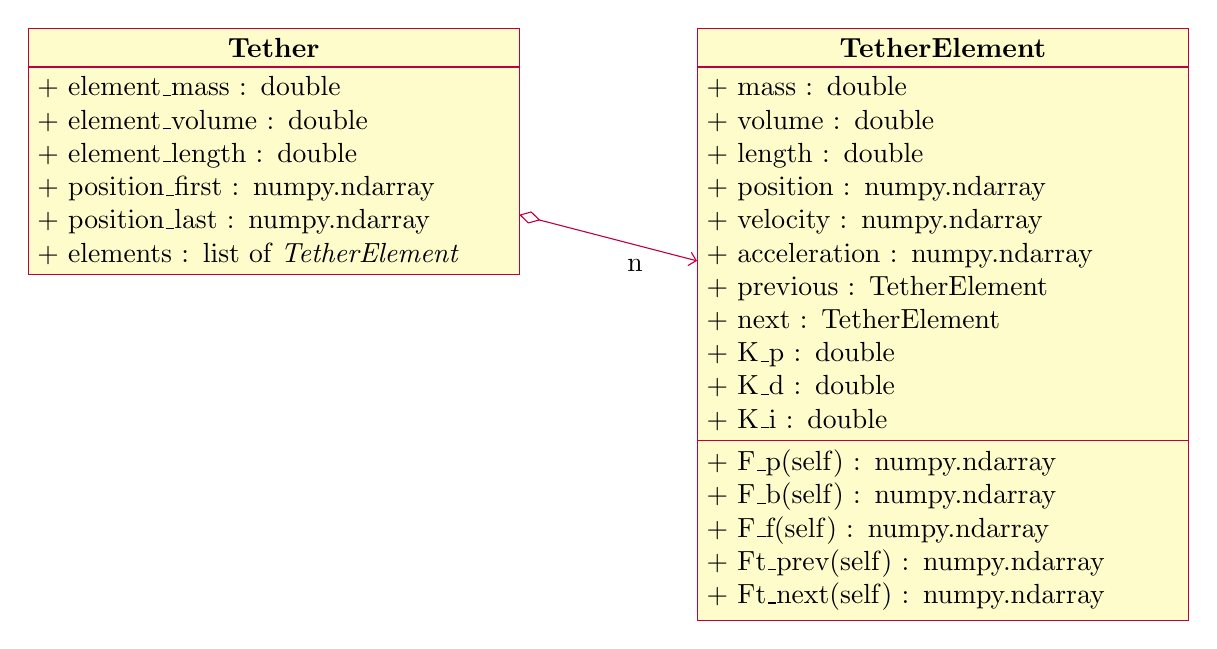
\begin{tikzpicture}
            \begin{class}[text width=6cm]{Tether}{0,0}
                \attribute{+ element\_mass : double}
                \attribute{+ element\_volume : double}
                \attribute{+ element\_length : double}
                \attribute{+ position\_first : numpy.ndarray}
                \attribute{+ position\_last : numpy.ndarray}
                \attribute{+ elements : list of \textit{TetherElement}}
            \end{class}
        
            \begin{class}[text width=6cm]{TetherElement}{8.5,0}
                \attribute{+ mass : double}
                \attribute{+ volume : double}
                \attribute{+ length : double}
                \attribute{+ position : numpy.ndarray}
                \attribute{+ velocity : numpy.ndarray}
                \attribute{+ acceleration : numpy.ndarray}
                \attribute{+ previous : TetherElement}
                \attribute{+ next : TetherElement}
                \attribute{+ K\_p : double}TetherElement
                \attribute{+ K\_d : double}
                \attribute{+ K\_i : double}
                \operation{+ F\_p(self) : numpy.ndarray}
                \operation{+ F\_b(self) : numpy.ndarray}
                \operation{+ F\_f(self) : numpy.ndarray}
                \operation{+ Ft\_prev(self) : numpy.ndarray}
                \operation{+ Ft\_next(self) : numpy.ndarray}
            \end{class}
        
            \aggregation{Tether}{}{~~~n}{TetherElement}
        \end{tikzpicture}
    }
    \caption{UML diagram of the \textit{Tether} and \textit{TetherElement} classes}
    \label{fig:uml}
\end{figure}


	\section{Initialization}
	\label{sec:initialization}
	Initialization is an important step because if the initial position of each TetherElement is random, the Tether will take a long time to converge and the system will be inconsistent. This is mainly due to the fact that the coefficients of the behavioral model are set to keep the nodes at a good distance from each other when a small perturbation is brought to the system.

To initialize the different nodes, we use the catenary equation~\cite{obrien_general_1968}~\cite{ren_parabolic_2008}. The idea is to use the shape taken by a rope attached at the ends to two fixed coordinate points. This rope will want to minimize its energy and so it takes this shape. This chain should check the following second order differential equation.

$$\ddot{z} = \frac{1}{k} \cdot \sqrt{1 + \dot{z}}$$

The solutions are known~\cite{obrien_general_1968}~\cite{ren_parabolic_2008} and of the form :

$$z(x) = k \cdot cosh\left(\frac{x}{k}\right)$$

However, this solution shows a rope centered around the ordinate axis. This is not necessarily a situation that we will find in our simulation. Here we would like to set the two fixed extremities, noted $(x_1, y_1, z_1)$ and $(x_n, y_n, z_n)$. By introducing $c_1$, $c_2$ and $c_3$ three coefficients allowing to correctly place the rope~\cite{ren_parabolic_2008}, we will then want to find here an equation of the form :

$$z(x) = c_1 \cdot cosh\left(\frac{x+c_2}{c_1}\right)+c_3$$

To find these coefficients, we have at our disposal three conditions: the two conditions related to the end points and the length of the string which must be equal to $L$. These conditions are expressed by the following equations:

\begin{align*}
    L = & c_1 \cdot sinh\left(\dfrac{x_n+c_2}{c_1}\right) - c_1 \cdot sinh\left(\dfrac{x_1+c_2}{c_1}\right) \\
    z_1 = & c_1 \cdot cosh\left(\dfrac{x_1+c_2}{c_1}\right)+c_3 \\
    z_n = & c_1 \cdot cosh\left(\dfrac{x_n+c_2}{c_1}\right)+c_3
\end{align*}

It is possible to solve the system of equations numerically using the function \textit{fsolve} of the package \textit{scipy.optimize}~\cite{noauthor_scipyorg_nodate}. Finally, from the calculated coefficients, and by knowing the length between the first node and the $i^{th}$ node, it is possible to initialize the nodes by reusing the previous constraints but the unknowns become the position $x_i$ and $z_i$. Note that the constraint on the position of the first node brings nothing to the system of equations, which leads to a system of two equations with two unknowns. The $y_i$ of each TetherElement are linearly spaced between the two extremities.

	\section{Results}
	\label{sec:results}
	This section will present the results of the simulation. To set the different coefficients of the simulation, we will need to build some tools to evaluate the performance of such a model~\cite{ellis_modeling_nodate}.

\subsection{Length of different links}

It is useful to trace the length of the links over time in order to verify that the Tether's behavioral model is correct.

The \textsc{Figure}~\ref{fig:length} shows in gray the plot of the length of each link for a simulation containing 15 nodes. In crimson is plotted the average of these lengths and in yellow the target length. Finally, the blue area shows the 95 \% confidence interval.

\begin{figure}[!htb]
    \centering
    %% Creator: Matplotlib, PGF backend
%%
%% To include the figure in your LaTeX document, write
%%   \input{<filename>.pgf}
%%
%% Make sure the required packages are loaded in your preamble
%%   \usepackage{pgf}
%%
%% and, on pdftex
%%   \usepackage[utf8]{inputenc}\DeclareUnicodeCharacter{2212}{-}
%%
%% or, on luatex and xetex
%%   \usepackage{unicode-math}
%%
%% Figures using additional raster images can only be included by \input if
%% they are in the same directory as the main LaTeX file. For loading figures
%% from other directories you can use the `import` package
%%   \usepackage{import}
%%
%% and then include the figures with
%%   \import{<path to file>}{<filename>.pgf}
%%
%% Matplotlib used the following preamble
%%
\begingroup%
\makeatletter%
\begin{pgfpicture}%
\pgfpathrectangle{\pgfpointorigin}{\pgfqpoint{3.500000in}{2.800000in}}%
\pgfusepath{use as bounding box, clip}%
\begin{pgfscope}%
\pgfsetbuttcap%
\pgfsetmiterjoin%
\definecolor{currentfill}{rgb}{1.000000,1.000000,1.000000}%
\pgfsetfillcolor{currentfill}%
\pgfsetlinewidth{0.000000pt}%
\definecolor{currentstroke}{rgb}{1.000000,1.000000,1.000000}%
\pgfsetstrokecolor{currentstroke}%
\pgfsetdash{}{0pt}%
\pgfpathmoveto{\pgfqpoint{0.000000in}{0.000000in}}%
\pgfpathlineto{\pgfqpoint{3.500000in}{0.000000in}}%
\pgfpathlineto{\pgfqpoint{3.500000in}{2.800000in}}%
\pgfpathlineto{\pgfqpoint{0.000000in}{2.800000in}}%
\pgfpathclose%
\pgfusepath{fill}%
\end{pgfscope}%
\begin{pgfscope}%
\pgfsetbuttcap%
\pgfsetmiterjoin%
\definecolor{currentfill}{rgb}{1.000000,1.000000,1.000000}%
\pgfsetfillcolor{currentfill}%
\pgfsetlinewidth{0.000000pt}%
\definecolor{currentstroke}{rgb}{0.000000,0.000000,0.000000}%
\pgfsetstrokecolor{currentstroke}%
\pgfsetstrokeopacity{0.000000}%
\pgfsetdash{}{0pt}%
\pgfpathmoveto{\pgfqpoint{0.580556in}{0.565123in}}%
\pgfpathlineto{\pgfqpoint{3.280555in}{0.565123in}}%
\pgfpathlineto{\pgfqpoint{3.280555in}{2.605271in}}%
\pgfpathlineto{\pgfqpoint{0.580556in}{2.605271in}}%
\pgfpathclose%
\pgfusepath{fill}%
\end{pgfscope}%
\begin{pgfscope}%
\pgfpathrectangle{\pgfqpoint{0.580556in}{0.565123in}}{\pgfqpoint{2.699999in}{2.040147in}}%
\pgfusepath{clip}%
\pgfsetbuttcap%
\pgfsetroundjoin%
\definecolor{currentfill}{rgb}{0.000000,0.501961,0.501961}%
\pgfsetfillcolor{currentfill}%
\pgfsetfillopacity{0.400000}%
\pgfsetlinewidth{0.000000pt}%
\definecolor{currentstroke}{rgb}{0.000000,0.000000,0.000000}%
\pgfsetstrokecolor{currentstroke}%
\pgfsetdash{}{0pt}%
\pgfpathmoveto{\pgfqpoint{0.580556in}{2.503310in}}%
\pgfpathlineto{\pgfqpoint{0.580556in}{0.657857in}}%
\pgfpathlineto{\pgfqpoint{0.585056in}{0.657857in}}%
\pgfpathlineto{\pgfqpoint{0.589556in}{0.657857in}}%
\pgfpathlineto{\pgfqpoint{0.594056in}{0.657857in}}%
\pgfpathlineto{\pgfqpoint{0.598556in}{0.657857in}}%
\pgfpathlineto{\pgfqpoint{0.603056in}{0.657857in}}%
\pgfpathlineto{\pgfqpoint{0.607556in}{0.657857in}}%
\pgfpathlineto{\pgfqpoint{0.612056in}{0.657857in}}%
\pgfpathlineto{\pgfqpoint{0.616556in}{0.657857in}}%
\pgfpathlineto{\pgfqpoint{0.621056in}{0.657857in}}%
\pgfpathlineto{\pgfqpoint{0.625556in}{0.657857in}}%
\pgfpathlineto{\pgfqpoint{0.630056in}{0.657857in}}%
\pgfpathlineto{\pgfqpoint{0.634556in}{0.657857in}}%
\pgfpathlineto{\pgfqpoint{0.639056in}{0.657857in}}%
\pgfpathlineto{\pgfqpoint{0.643556in}{0.657857in}}%
\pgfpathlineto{\pgfqpoint{0.648056in}{0.657857in}}%
\pgfpathlineto{\pgfqpoint{0.652556in}{0.657857in}}%
\pgfpathlineto{\pgfqpoint{0.657056in}{0.657857in}}%
\pgfpathlineto{\pgfqpoint{0.661556in}{0.657857in}}%
\pgfpathlineto{\pgfqpoint{0.666056in}{0.657857in}}%
\pgfpathlineto{\pgfqpoint{0.670556in}{0.657857in}}%
\pgfpathlineto{\pgfqpoint{0.675056in}{0.657857in}}%
\pgfpathlineto{\pgfqpoint{0.679556in}{0.657857in}}%
\pgfpathlineto{\pgfqpoint{0.684056in}{0.661041in}}%
\pgfpathlineto{\pgfqpoint{0.688556in}{0.678385in}}%
\pgfpathlineto{\pgfqpoint{0.693056in}{0.692815in}}%
\pgfpathlineto{\pgfqpoint{0.697556in}{0.704235in}}%
\pgfpathlineto{\pgfqpoint{0.702056in}{0.712618in}}%
\pgfpathlineto{\pgfqpoint{0.706556in}{0.718018in}}%
\pgfpathlineto{\pgfqpoint{0.711056in}{0.720567in}}%
\pgfpathlineto{\pgfqpoint{0.715556in}{0.720465in}}%
\pgfpathlineto{\pgfqpoint{0.720056in}{0.717952in}}%
\pgfpathlineto{\pgfqpoint{0.724556in}{0.713278in}}%
\pgfpathlineto{\pgfqpoint{0.729056in}{0.706682in}}%
\pgfpathlineto{\pgfqpoint{0.733556in}{0.698391in}}%
\pgfpathlineto{\pgfqpoint{0.738056in}{0.688628in}}%
\pgfpathlineto{\pgfqpoint{0.742556in}{0.677621in}}%
\pgfpathlineto{\pgfqpoint{0.747056in}{0.665613in}}%
\pgfpathlineto{\pgfqpoint{0.751556in}{0.657857in}}%
\pgfpathlineto{\pgfqpoint{0.756056in}{0.657857in}}%
\pgfpathlineto{\pgfqpoint{0.760556in}{0.657857in}}%
\pgfpathlineto{\pgfqpoint{0.765056in}{0.657857in}}%
\pgfpathlineto{\pgfqpoint{0.769556in}{0.657857in}}%
\pgfpathlineto{\pgfqpoint{0.774056in}{0.657857in}}%
\pgfpathlineto{\pgfqpoint{0.778556in}{0.657857in}}%
\pgfpathlineto{\pgfqpoint{0.783056in}{0.657857in}}%
\pgfpathlineto{\pgfqpoint{0.787556in}{0.657857in}}%
\pgfpathlineto{\pgfqpoint{0.792056in}{0.657857in}}%
\pgfpathlineto{\pgfqpoint{0.796556in}{0.657857in}}%
\pgfpathlineto{\pgfqpoint{0.801056in}{0.657857in}}%
\pgfpathlineto{\pgfqpoint{0.805556in}{0.657857in}}%
\pgfpathlineto{\pgfqpoint{0.810056in}{0.657857in}}%
\pgfpathlineto{\pgfqpoint{0.814556in}{0.657857in}}%
\pgfpathlineto{\pgfqpoint{0.819056in}{0.657857in}}%
\pgfpathlineto{\pgfqpoint{0.823556in}{0.657857in}}%
\pgfpathlineto{\pgfqpoint{0.828056in}{0.657857in}}%
\pgfpathlineto{\pgfqpoint{0.832556in}{0.657857in}}%
\pgfpathlineto{\pgfqpoint{0.837056in}{0.657857in}}%
\pgfpathlineto{\pgfqpoint{0.841556in}{0.657857in}}%
\pgfpathlineto{\pgfqpoint{0.846056in}{0.657857in}}%
\pgfpathlineto{\pgfqpoint{0.850556in}{0.657857in}}%
\pgfpathlineto{\pgfqpoint{0.855056in}{0.657857in}}%
\pgfpathlineto{\pgfqpoint{0.859556in}{0.657857in}}%
\pgfpathlineto{\pgfqpoint{0.864056in}{0.657857in}}%
\pgfpathlineto{\pgfqpoint{0.868556in}{0.657857in}}%
\pgfpathlineto{\pgfqpoint{0.873056in}{0.657857in}}%
\pgfpathlineto{\pgfqpoint{0.877556in}{0.657857in}}%
\pgfpathlineto{\pgfqpoint{0.882056in}{0.657857in}}%
\pgfpathlineto{\pgfqpoint{0.886556in}{0.657857in}}%
\pgfpathlineto{\pgfqpoint{0.891056in}{0.657857in}}%
\pgfpathlineto{\pgfqpoint{0.895556in}{0.657857in}}%
\pgfpathlineto{\pgfqpoint{0.900056in}{0.657857in}}%
\pgfpathlineto{\pgfqpoint{0.904556in}{0.657857in}}%
\pgfpathlineto{\pgfqpoint{0.909056in}{0.657857in}}%
\pgfpathlineto{\pgfqpoint{0.913556in}{0.657857in}}%
\pgfpathlineto{\pgfqpoint{0.918056in}{0.657857in}}%
\pgfpathlineto{\pgfqpoint{0.922556in}{0.657857in}}%
\pgfpathlineto{\pgfqpoint{0.927056in}{0.657857in}}%
\pgfpathlineto{\pgfqpoint{0.931556in}{0.657857in}}%
\pgfpathlineto{\pgfqpoint{0.936056in}{0.657857in}}%
\pgfpathlineto{\pgfqpoint{0.940556in}{0.657857in}}%
\pgfpathlineto{\pgfqpoint{0.945056in}{0.657857in}}%
\pgfpathlineto{\pgfqpoint{0.949556in}{0.657857in}}%
\pgfpathlineto{\pgfqpoint{0.954056in}{0.657857in}}%
\pgfpathlineto{\pgfqpoint{0.958556in}{0.657857in}}%
\pgfpathlineto{\pgfqpoint{0.963056in}{0.657857in}}%
\pgfpathlineto{\pgfqpoint{0.967556in}{0.657857in}}%
\pgfpathlineto{\pgfqpoint{0.972056in}{0.657857in}}%
\pgfpathlineto{\pgfqpoint{0.976556in}{0.657857in}}%
\pgfpathlineto{\pgfqpoint{0.981056in}{0.657857in}}%
\pgfpathlineto{\pgfqpoint{0.985556in}{0.657857in}}%
\pgfpathlineto{\pgfqpoint{0.990056in}{0.657857in}}%
\pgfpathlineto{\pgfqpoint{0.994556in}{0.657857in}}%
\pgfpathlineto{\pgfqpoint{0.999056in}{0.657857in}}%
\pgfpathlineto{\pgfqpoint{1.003556in}{0.657857in}}%
\pgfpathlineto{\pgfqpoint{1.008056in}{0.657857in}}%
\pgfpathlineto{\pgfqpoint{1.012556in}{0.657857in}}%
\pgfpathlineto{\pgfqpoint{1.017056in}{0.657857in}}%
\pgfpathlineto{\pgfqpoint{1.021556in}{0.657857in}}%
\pgfpathlineto{\pgfqpoint{1.026056in}{0.657857in}}%
\pgfpathlineto{\pgfqpoint{1.030556in}{0.657857in}}%
\pgfpathlineto{\pgfqpoint{1.035056in}{0.657857in}}%
\pgfpathlineto{\pgfqpoint{1.039556in}{0.657857in}}%
\pgfpathlineto{\pgfqpoint{1.044056in}{0.657857in}}%
\pgfpathlineto{\pgfqpoint{1.048556in}{0.657857in}}%
\pgfpathlineto{\pgfqpoint{1.053056in}{0.657857in}}%
\pgfpathlineto{\pgfqpoint{1.057556in}{0.657857in}}%
\pgfpathlineto{\pgfqpoint{1.062056in}{0.657857in}}%
\pgfpathlineto{\pgfqpoint{1.066556in}{0.657857in}}%
\pgfpathlineto{\pgfqpoint{1.071056in}{0.657857in}}%
\pgfpathlineto{\pgfqpoint{1.075556in}{0.657857in}}%
\pgfpathlineto{\pgfqpoint{1.080056in}{0.657857in}}%
\pgfpathlineto{\pgfqpoint{1.084556in}{0.657857in}}%
\pgfpathlineto{\pgfqpoint{1.089056in}{0.657857in}}%
\pgfpathlineto{\pgfqpoint{1.093556in}{0.657857in}}%
\pgfpathlineto{\pgfqpoint{1.098056in}{0.657857in}}%
\pgfpathlineto{\pgfqpoint{1.102556in}{0.657857in}}%
\pgfpathlineto{\pgfqpoint{1.107056in}{0.657857in}}%
\pgfpathlineto{\pgfqpoint{1.111556in}{0.657857in}}%
\pgfpathlineto{\pgfqpoint{1.116056in}{0.657857in}}%
\pgfpathlineto{\pgfqpoint{1.120556in}{0.657857in}}%
\pgfpathlineto{\pgfqpoint{1.125056in}{0.657857in}}%
\pgfpathlineto{\pgfqpoint{1.129556in}{0.657857in}}%
\pgfpathlineto{\pgfqpoint{1.134056in}{0.657857in}}%
\pgfpathlineto{\pgfqpoint{1.138556in}{0.657857in}}%
\pgfpathlineto{\pgfqpoint{1.143056in}{0.657857in}}%
\pgfpathlineto{\pgfqpoint{1.147556in}{0.657857in}}%
\pgfpathlineto{\pgfqpoint{1.152056in}{0.657857in}}%
\pgfpathlineto{\pgfqpoint{1.156556in}{0.657857in}}%
\pgfpathlineto{\pgfqpoint{1.161056in}{0.657857in}}%
\pgfpathlineto{\pgfqpoint{1.165556in}{0.657857in}}%
\pgfpathlineto{\pgfqpoint{1.170056in}{0.657857in}}%
\pgfpathlineto{\pgfqpoint{1.174556in}{0.657857in}}%
\pgfpathlineto{\pgfqpoint{1.179056in}{0.657857in}}%
\pgfpathlineto{\pgfqpoint{1.183556in}{0.657857in}}%
\pgfpathlineto{\pgfqpoint{1.188056in}{0.657857in}}%
\pgfpathlineto{\pgfqpoint{1.192556in}{0.657857in}}%
\pgfpathlineto{\pgfqpoint{1.197056in}{0.657857in}}%
\pgfpathlineto{\pgfqpoint{1.201556in}{0.657857in}}%
\pgfpathlineto{\pgfqpoint{1.206056in}{0.657857in}}%
\pgfpathlineto{\pgfqpoint{1.210556in}{0.657857in}}%
\pgfpathlineto{\pgfqpoint{1.215056in}{0.657857in}}%
\pgfpathlineto{\pgfqpoint{1.219556in}{0.657857in}}%
\pgfpathlineto{\pgfqpoint{1.224056in}{0.657857in}}%
\pgfpathlineto{\pgfqpoint{1.228556in}{0.657857in}}%
\pgfpathlineto{\pgfqpoint{1.233056in}{0.657857in}}%
\pgfpathlineto{\pgfqpoint{1.237556in}{0.657857in}}%
\pgfpathlineto{\pgfqpoint{1.242056in}{0.657857in}}%
\pgfpathlineto{\pgfqpoint{1.246556in}{0.657857in}}%
\pgfpathlineto{\pgfqpoint{1.251056in}{0.657857in}}%
\pgfpathlineto{\pgfqpoint{1.255556in}{0.657857in}}%
\pgfpathlineto{\pgfqpoint{1.260056in}{0.657857in}}%
\pgfpathlineto{\pgfqpoint{1.264556in}{0.657857in}}%
\pgfpathlineto{\pgfqpoint{1.269056in}{0.657857in}}%
\pgfpathlineto{\pgfqpoint{1.273556in}{0.657857in}}%
\pgfpathlineto{\pgfqpoint{1.278056in}{0.657857in}}%
\pgfpathlineto{\pgfqpoint{1.282556in}{0.657857in}}%
\pgfpathlineto{\pgfqpoint{1.287056in}{0.657857in}}%
\pgfpathlineto{\pgfqpoint{1.291556in}{0.657857in}}%
\pgfpathlineto{\pgfqpoint{1.296056in}{0.657857in}}%
\pgfpathlineto{\pgfqpoint{1.300556in}{0.657857in}}%
\pgfpathlineto{\pgfqpoint{1.305056in}{0.657857in}}%
\pgfpathlineto{\pgfqpoint{1.309556in}{0.657857in}}%
\pgfpathlineto{\pgfqpoint{1.314056in}{0.657857in}}%
\pgfpathlineto{\pgfqpoint{1.318556in}{0.657857in}}%
\pgfpathlineto{\pgfqpoint{1.323056in}{0.657857in}}%
\pgfpathlineto{\pgfqpoint{1.327556in}{0.657857in}}%
\pgfpathlineto{\pgfqpoint{1.332056in}{0.657857in}}%
\pgfpathlineto{\pgfqpoint{1.336556in}{0.657857in}}%
\pgfpathlineto{\pgfqpoint{1.341056in}{0.657857in}}%
\pgfpathlineto{\pgfqpoint{1.345556in}{0.657857in}}%
\pgfpathlineto{\pgfqpoint{1.350056in}{0.657857in}}%
\pgfpathlineto{\pgfqpoint{1.354556in}{0.657857in}}%
\pgfpathlineto{\pgfqpoint{1.359056in}{0.657857in}}%
\pgfpathlineto{\pgfqpoint{1.363556in}{0.657857in}}%
\pgfpathlineto{\pgfqpoint{1.368056in}{0.657857in}}%
\pgfpathlineto{\pgfqpoint{1.372556in}{0.657857in}}%
\pgfpathlineto{\pgfqpoint{1.377056in}{0.657857in}}%
\pgfpathlineto{\pgfqpoint{1.381556in}{0.657857in}}%
\pgfpathlineto{\pgfqpoint{1.386056in}{0.657857in}}%
\pgfpathlineto{\pgfqpoint{1.390556in}{0.657857in}}%
\pgfpathlineto{\pgfqpoint{1.395056in}{0.657857in}}%
\pgfpathlineto{\pgfqpoint{1.399556in}{0.657857in}}%
\pgfpathlineto{\pgfqpoint{1.404056in}{0.657857in}}%
\pgfpathlineto{\pgfqpoint{1.408556in}{0.657857in}}%
\pgfpathlineto{\pgfqpoint{1.413056in}{0.657857in}}%
\pgfpathlineto{\pgfqpoint{1.417556in}{0.657857in}}%
\pgfpathlineto{\pgfqpoint{1.422056in}{0.657857in}}%
\pgfpathlineto{\pgfqpoint{1.426556in}{0.657857in}}%
\pgfpathlineto{\pgfqpoint{1.431056in}{0.657857in}}%
\pgfpathlineto{\pgfqpoint{1.435556in}{0.657857in}}%
\pgfpathlineto{\pgfqpoint{1.440056in}{0.657857in}}%
\pgfpathlineto{\pgfqpoint{1.444556in}{0.657857in}}%
\pgfpathlineto{\pgfqpoint{1.449056in}{0.657857in}}%
\pgfpathlineto{\pgfqpoint{1.453556in}{0.657857in}}%
\pgfpathlineto{\pgfqpoint{1.458056in}{0.657857in}}%
\pgfpathlineto{\pgfqpoint{1.462556in}{0.657857in}}%
\pgfpathlineto{\pgfqpoint{1.467056in}{0.657857in}}%
\pgfpathlineto{\pgfqpoint{1.471556in}{0.657857in}}%
\pgfpathlineto{\pgfqpoint{1.476056in}{0.657857in}}%
\pgfpathlineto{\pgfqpoint{1.480556in}{0.657857in}}%
\pgfpathlineto{\pgfqpoint{1.485056in}{0.657857in}}%
\pgfpathlineto{\pgfqpoint{1.489556in}{0.657857in}}%
\pgfpathlineto{\pgfqpoint{1.494056in}{0.657857in}}%
\pgfpathlineto{\pgfqpoint{1.498556in}{0.657857in}}%
\pgfpathlineto{\pgfqpoint{1.503056in}{0.657857in}}%
\pgfpathlineto{\pgfqpoint{1.507556in}{0.657857in}}%
\pgfpathlineto{\pgfqpoint{1.512056in}{0.657857in}}%
\pgfpathlineto{\pgfqpoint{1.516556in}{0.657857in}}%
\pgfpathlineto{\pgfqpoint{1.521056in}{0.657857in}}%
\pgfpathlineto{\pgfqpoint{1.525556in}{0.657857in}}%
\pgfpathlineto{\pgfqpoint{1.530056in}{0.657857in}}%
\pgfpathlineto{\pgfqpoint{1.534556in}{0.657857in}}%
\pgfpathlineto{\pgfqpoint{1.539056in}{0.657857in}}%
\pgfpathlineto{\pgfqpoint{1.543556in}{0.657857in}}%
\pgfpathlineto{\pgfqpoint{1.548056in}{0.657857in}}%
\pgfpathlineto{\pgfqpoint{1.552556in}{0.657857in}}%
\pgfpathlineto{\pgfqpoint{1.557056in}{0.657857in}}%
\pgfpathlineto{\pgfqpoint{1.561556in}{0.657857in}}%
\pgfpathlineto{\pgfqpoint{1.566056in}{0.657857in}}%
\pgfpathlineto{\pgfqpoint{1.570556in}{0.657857in}}%
\pgfpathlineto{\pgfqpoint{1.575056in}{0.657857in}}%
\pgfpathlineto{\pgfqpoint{1.579556in}{0.657857in}}%
\pgfpathlineto{\pgfqpoint{1.584056in}{0.657857in}}%
\pgfpathlineto{\pgfqpoint{1.588556in}{0.657857in}}%
\pgfpathlineto{\pgfqpoint{1.593056in}{0.657857in}}%
\pgfpathlineto{\pgfqpoint{1.597556in}{0.657857in}}%
\pgfpathlineto{\pgfqpoint{1.602056in}{0.657857in}}%
\pgfpathlineto{\pgfqpoint{1.606556in}{0.657857in}}%
\pgfpathlineto{\pgfqpoint{1.611056in}{0.657857in}}%
\pgfpathlineto{\pgfqpoint{1.615556in}{0.657857in}}%
\pgfpathlineto{\pgfqpoint{1.620056in}{0.657857in}}%
\pgfpathlineto{\pgfqpoint{1.624556in}{0.657857in}}%
\pgfpathlineto{\pgfqpoint{1.629056in}{0.657857in}}%
\pgfpathlineto{\pgfqpoint{1.633556in}{0.657857in}}%
\pgfpathlineto{\pgfqpoint{1.638056in}{0.657857in}}%
\pgfpathlineto{\pgfqpoint{1.642556in}{0.657857in}}%
\pgfpathlineto{\pgfqpoint{1.647056in}{0.657857in}}%
\pgfpathlineto{\pgfqpoint{1.651556in}{0.657857in}}%
\pgfpathlineto{\pgfqpoint{1.656056in}{0.657857in}}%
\pgfpathlineto{\pgfqpoint{1.660556in}{0.657857in}}%
\pgfpathlineto{\pgfqpoint{1.665056in}{0.657857in}}%
\pgfpathlineto{\pgfqpoint{1.669556in}{0.657857in}}%
\pgfpathlineto{\pgfqpoint{1.674056in}{0.657857in}}%
\pgfpathlineto{\pgfqpoint{1.678556in}{0.657857in}}%
\pgfpathlineto{\pgfqpoint{1.683056in}{0.657857in}}%
\pgfpathlineto{\pgfqpoint{1.687556in}{0.657857in}}%
\pgfpathlineto{\pgfqpoint{1.692056in}{0.657857in}}%
\pgfpathlineto{\pgfqpoint{1.696556in}{0.657857in}}%
\pgfpathlineto{\pgfqpoint{1.701056in}{0.657857in}}%
\pgfpathlineto{\pgfqpoint{1.705556in}{0.657857in}}%
\pgfpathlineto{\pgfqpoint{1.710056in}{0.657857in}}%
\pgfpathlineto{\pgfqpoint{1.714556in}{0.657857in}}%
\pgfpathlineto{\pgfqpoint{1.719056in}{0.657857in}}%
\pgfpathlineto{\pgfqpoint{1.723556in}{0.657857in}}%
\pgfpathlineto{\pgfqpoint{1.728056in}{0.657857in}}%
\pgfpathlineto{\pgfqpoint{1.732556in}{0.657857in}}%
\pgfpathlineto{\pgfqpoint{1.737056in}{0.657857in}}%
\pgfpathlineto{\pgfqpoint{1.741556in}{0.657857in}}%
\pgfpathlineto{\pgfqpoint{1.746056in}{0.657857in}}%
\pgfpathlineto{\pgfqpoint{1.750556in}{0.657857in}}%
\pgfpathlineto{\pgfqpoint{1.755056in}{0.657857in}}%
\pgfpathlineto{\pgfqpoint{1.759556in}{0.657857in}}%
\pgfpathlineto{\pgfqpoint{1.764056in}{0.657857in}}%
\pgfpathlineto{\pgfqpoint{1.768556in}{0.657857in}}%
\pgfpathlineto{\pgfqpoint{1.773056in}{0.657857in}}%
\pgfpathlineto{\pgfqpoint{1.777556in}{0.657857in}}%
\pgfpathlineto{\pgfqpoint{1.782056in}{0.657857in}}%
\pgfpathlineto{\pgfqpoint{1.786556in}{0.657857in}}%
\pgfpathlineto{\pgfqpoint{1.791056in}{0.657857in}}%
\pgfpathlineto{\pgfqpoint{1.795556in}{0.657857in}}%
\pgfpathlineto{\pgfqpoint{1.800056in}{0.657857in}}%
\pgfpathlineto{\pgfqpoint{1.804556in}{0.657857in}}%
\pgfpathlineto{\pgfqpoint{1.809056in}{0.657857in}}%
\pgfpathlineto{\pgfqpoint{1.813556in}{0.657857in}}%
\pgfpathlineto{\pgfqpoint{1.818056in}{0.657857in}}%
\pgfpathlineto{\pgfqpoint{1.822556in}{0.657857in}}%
\pgfpathlineto{\pgfqpoint{1.827056in}{0.657857in}}%
\pgfpathlineto{\pgfqpoint{1.831556in}{0.657857in}}%
\pgfpathlineto{\pgfqpoint{1.836056in}{0.657857in}}%
\pgfpathlineto{\pgfqpoint{1.840556in}{0.657857in}}%
\pgfpathlineto{\pgfqpoint{1.845056in}{0.657857in}}%
\pgfpathlineto{\pgfqpoint{1.849556in}{0.657857in}}%
\pgfpathlineto{\pgfqpoint{1.854056in}{0.657857in}}%
\pgfpathlineto{\pgfqpoint{1.858556in}{0.657857in}}%
\pgfpathlineto{\pgfqpoint{1.863056in}{0.657857in}}%
\pgfpathlineto{\pgfqpoint{1.867556in}{0.657857in}}%
\pgfpathlineto{\pgfqpoint{1.872056in}{0.657857in}}%
\pgfpathlineto{\pgfqpoint{1.876556in}{0.657857in}}%
\pgfpathlineto{\pgfqpoint{1.881056in}{0.657857in}}%
\pgfpathlineto{\pgfqpoint{1.885556in}{0.657857in}}%
\pgfpathlineto{\pgfqpoint{1.890056in}{0.657857in}}%
\pgfpathlineto{\pgfqpoint{1.894556in}{0.657857in}}%
\pgfpathlineto{\pgfqpoint{1.899056in}{0.657857in}}%
\pgfpathlineto{\pgfqpoint{1.903556in}{0.657857in}}%
\pgfpathlineto{\pgfqpoint{1.908056in}{0.657857in}}%
\pgfpathlineto{\pgfqpoint{1.912556in}{0.657857in}}%
\pgfpathlineto{\pgfqpoint{1.917056in}{0.657857in}}%
\pgfpathlineto{\pgfqpoint{1.921556in}{0.657857in}}%
\pgfpathlineto{\pgfqpoint{1.926056in}{0.657857in}}%
\pgfpathlineto{\pgfqpoint{1.930556in}{0.657857in}}%
\pgfpathlineto{\pgfqpoint{1.935056in}{0.657857in}}%
\pgfpathlineto{\pgfqpoint{1.939556in}{0.657857in}}%
\pgfpathlineto{\pgfqpoint{1.944056in}{0.657857in}}%
\pgfpathlineto{\pgfqpoint{1.948556in}{0.657857in}}%
\pgfpathlineto{\pgfqpoint{1.953056in}{0.657857in}}%
\pgfpathlineto{\pgfqpoint{1.957556in}{0.657857in}}%
\pgfpathlineto{\pgfqpoint{1.962056in}{0.657857in}}%
\pgfpathlineto{\pgfqpoint{1.966556in}{0.657857in}}%
\pgfpathlineto{\pgfqpoint{1.971056in}{0.657857in}}%
\pgfpathlineto{\pgfqpoint{1.975556in}{0.657857in}}%
\pgfpathlineto{\pgfqpoint{1.980056in}{0.657857in}}%
\pgfpathlineto{\pgfqpoint{1.984556in}{0.657857in}}%
\pgfpathlineto{\pgfqpoint{1.989056in}{0.657857in}}%
\pgfpathlineto{\pgfqpoint{1.993556in}{0.657857in}}%
\pgfpathlineto{\pgfqpoint{1.998056in}{0.657857in}}%
\pgfpathlineto{\pgfqpoint{2.002556in}{0.657857in}}%
\pgfpathlineto{\pgfqpoint{2.007056in}{0.657857in}}%
\pgfpathlineto{\pgfqpoint{2.011556in}{0.657857in}}%
\pgfpathlineto{\pgfqpoint{2.016056in}{0.657857in}}%
\pgfpathlineto{\pgfqpoint{2.020556in}{0.657857in}}%
\pgfpathlineto{\pgfqpoint{2.025056in}{0.657857in}}%
\pgfpathlineto{\pgfqpoint{2.029556in}{0.657857in}}%
\pgfpathlineto{\pgfqpoint{2.034056in}{0.657857in}}%
\pgfpathlineto{\pgfqpoint{2.038556in}{0.657857in}}%
\pgfpathlineto{\pgfqpoint{2.043056in}{0.657857in}}%
\pgfpathlineto{\pgfqpoint{2.047556in}{0.657857in}}%
\pgfpathlineto{\pgfqpoint{2.052056in}{0.657857in}}%
\pgfpathlineto{\pgfqpoint{2.056556in}{0.657857in}}%
\pgfpathlineto{\pgfqpoint{2.061056in}{0.657857in}}%
\pgfpathlineto{\pgfqpoint{2.065556in}{0.657857in}}%
\pgfpathlineto{\pgfqpoint{2.070056in}{0.657857in}}%
\pgfpathlineto{\pgfqpoint{2.074556in}{0.657857in}}%
\pgfpathlineto{\pgfqpoint{2.079056in}{0.657857in}}%
\pgfpathlineto{\pgfqpoint{2.083556in}{0.657857in}}%
\pgfpathlineto{\pgfqpoint{2.088056in}{0.657857in}}%
\pgfpathlineto{\pgfqpoint{2.092556in}{0.657857in}}%
\pgfpathlineto{\pgfqpoint{2.097056in}{0.657857in}}%
\pgfpathlineto{\pgfqpoint{2.101556in}{0.657857in}}%
\pgfpathlineto{\pgfqpoint{2.106056in}{0.657857in}}%
\pgfpathlineto{\pgfqpoint{2.110556in}{0.657857in}}%
\pgfpathlineto{\pgfqpoint{2.115056in}{0.657857in}}%
\pgfpathlineto{\pgfqpoint{2.119556in}{0.657857in}}%
\pgfpathlineto{\pgfqpoint{2.124056in}{0.657857in}}%
\pgfpathlineto{\pgfqpoint{2.128556in}{0.657857in}}%
\pgfpathlineto{\pgfqpoint{2.133056in}{0.657857in}}%
\pgfpathlineto{\pgfqpoint{2.137556in}{0.657857in}}%
\pgfpathlineto{\pgfqpoint{2.142056in}{0.657857in}}%
\pgfpathlineto{\pgfqpoint{2.146556in}{0.657857in}}%
\pgfpathlineto{\pgfqpoint{2.151056in}{0.657857in}}%
\pgfpathlineto{\pgfqpoint{2.155556in}{0.657857in}}%
\pgfpathlineto{\pgfqpoint{2.160056in}{0.657857in}}%
\pgfpathlineto{\pgfqpoint{2.164556in}{0.657857in}}%
\pgfpathlineto{\pgfqpoint{2.169056in}{0.657857in}}%
\pgfpathlineto{\pgfqpoint{2.173556in}{0.657857in}}%
\pgfpathlineto{\pgfqpoint{2.178056in}{0.657857in}}%
\pgfpathlineto{\pgfqpoint{2.182556in}{0.657857in}}%
\pgfpathlineto{\pgfqpoint{2.187056in}{0.657857in}}%
\pgfpathlineto{\pgfqpoint{2.191556in}{0.657857in}}%
\pgfpathlineto{\pgfqpoint{2.196056in}{0.657857in}}%
\pgfpathlineto{\pgfqpoint{2.200556in}{0.657857in}}%
\pgfpathlineto{\pgfqpoint{2.205056in}{0.657857in}}%
\pgfpathlineto{\pgfqpoint{2.209556in}{0.657857in}}%
\pgfpathlineto{\pgfqpoint{2.214056in}{0.657857in}}%
\pgfpathlineto{\pgfqpoint{2.218556in}{0.657857in}}%
\pgfpathlineto{\pgfqpoint{2.223056in}{0.657857in}}%
\pgfpathlineto{\pgfqpoint{2.227556in}{0.657857in}}%
\pgfpathlineto{\pgfqpoint{2.232056in}{0.657857in}}%
\pgfpathlineto{\pgfqpoint{2.236556in}{0.657857in}}%
\pgfpathlineto{\pgfqpoint{2.241056in}{0.657857in}}%
\pgfpathlineto{\pgfqpoint{2.245556in}{0.657857in}}%
\pgfpathlineto{\pgfqpoint{2.250056in}{0.657857in}}%
\pgfpathlineto{\pgfqpoint{2.254556in}{0.657857in}}%
\pgfpathlineto{\pgfqpoint{2.259056in}{0.657857in}}%
\pgfpathlineto{\pgfqpoint{2.263556in}{0.657857in}}%
\pgfpathlineto{\pgfqpoint{2.268056in}{0.657857in}}%
\pgfpathlineto{\pgfqpoint{2.272556in}{0.657857in}}%
\pgfpathlineto{\pgfqpoint{2.277056in}{0.657857in}}%
\pgfpathlineto{\pgfqpoint{2.281556in}{0.657857in}}%
\pgfpathlineto{\pgfqpoint{2.286056in}{0.657857in}}%
\pgfpathlineto{\pgfqpoint{2.290556in}{0.657857in}}%
\pgfpathlineto{\pgfqpoint{2.295056in}{0.657857in}}%
\pgfpathlineto{\pgfqpoint{2.299556in}{0.657857in}}%
\pgfpathlineto{\pgfqpoint{2.304056in}{0.657857in}}%
\pgfpathlineto{\pgfqpoint{2.308556in}{0.657857in}}%
\pgfpathlineto{\pgfqpoint{2.313056in}{0.657857in}}%
\pgfpathlineto{\pgfqpoint{2.317556in}{0.657857in}}%
\pgfpathlineto{\pgfqpoint{2.322056in}{0.657857in}}%
\pgfpathlineto{\pgfqpoint{2.326556in}{0.657857in}}%
\pgfpathlineto{\pgfqpoint{2.331056in}{0.657857in}}%
\pgfpathlineto{\pgfqpoint{2.335556in}{0.657857in}}%
\pgfpathlineto{\pgfqpoint{2.340056in}{0.657857in}}%
\pgfpathlineto{\pgfqpoint{2.344556in}{0.657857in}}%
\pgfpathlineto{\pgfqpoint{2.349056in}{0.657857in}}%
\pgfpathlineto{\pgfqpoint{2.353556in}{0.657857in}}%
\pgfpathlineto{\pgfqpoint{2.358056in}{0.657857in}}%
\pgfpathlineto{\pgfqpoint{2.362556in}{0.657857in}}%
\pgfpathlineto{\pgfqpoint{2.367056in}{0.657857in}}%
\pgfpathlineto{\pgfqpoint{2.371556in}{0.657857in}}%
\pgfpathlineto{\pgfqpoint{2.376056in}{0.657857in}}%
\pgfpathlineto{\pgfqpoint{2.380556in}{0.657857in}}%
\pgfpathlineto{\pgfqpoint{2.385056in}{0.657857in}}%
\pgfpathlineto{\pgfqpoint{2.389556in}{0.657857in}}%
\pgfpathlineto{\pgfqpoint{2.394056in}{0.657857in}}%
\pgfpathlineto{\pgfqpoint{2.398556in}{0.657857in}}%
\pgfpathlineto{\pgfqpoint{2.403056in}{0.657857in}}%
\pgfpathlineto{\pgfqpoint{2.407556in}{0.657857in}}%
\pgfpathlineto{\pgfqpoint{2.412056in}{0.657857in}}%
\pgfpathlineto{\pgfqpoint{2.416556in}{0.657857in}}%
\pgfpathlineto{\pgfqpoint{2.421056in}{0.657857in}}%
\pgfpathlineto{\pgfqpoint{2.425556in}{0.657857in}}%
\pgfpathlineto{\pgfqpoint{2.430056in}{0.657857in}}%
\pgfpathlineto{\pgfqpoint{2.434556in}{0.657857in}}%
\pgfpathlineto{\pgfqpoint{2.439056in}{0.657857in}}%
\pgfpathlineto{\pgfqpoint{2.443556in}{0.657857in}}%
\pgfpathlineto{\pgfqpoint{2.448056in}{0.657857in}}%
\pgfpathlineto{\pgfqpoint{2.452556in}{0.657857in}}%
\pgfpathlineto{\pgfqpoint{2.457056in}{0.657857in}}%
\pgfpathlineto{\pgfqpoint{2.461556in}{0.657857in}}%
\pgfpathlineto{\pgfqpoint{2.466056in}{0.657857in}}%
\pgfpathlineto{\pgfqpoint{2.470556in}{0.657857in}}%
\pgfpathlineto{\pgfqpoint{2.475056in}{0.657857in}}%
\pgfpathlineto{\pgfqpoint{2.479556in}{0.657857in}}%
\pgfpathlineto{\pgfqpoint{2.484056in}{0.657857in}}%
\pgfpathlineto{\pgfqpoint{2.488556in}{0.657857in}}%
\pgfpathlineto{\pgfqpoint{2.493056in}{0.657857in}}%
\pgfpathlineto{\pgfqpoint{2.497556in}{0.657857in}}%
\pgfpathlineto{\pgfqpoint{2.502056in}{0.657857in}}%
\pgfpathlineto{\pgfqpoint{2.506556in}{0.657857in}}%
\pgfpathlineto{\pgfqpoint{2.511056in}{0.657857in}}%
\pgfpathlineto{\pgfqpoint{2.515556in}{0.657857in}}%
\pgfpathlineto{\pgfqpoint{2.520056in}{0.657857in}}%
\pgfpathlineto{\pgfqpoint{2.524556in}{0.657857in}}%
\pgfpathlineto{\pgfqpoint{2.529056in}{0.657857in}}%
\pgfpathlineto{\pgfqpoint{2.533556in}{0.657857in}}%
\pgfpathlineto{\pgfqpoint{2.538056in}{0.657857in}}%
\pgfpathlineto{\pgfqpoint{2.542556in}{0.657857in}}%
\pgfpathlineto{\pgfqpoint{2.547056in}{0.657857in}}%
\pgfpathlineto{\pgfqpoint{2.551556in}{0.657857in}}%
\pgfpathlineto{\pgfqpoint{2.556056in}{0.657857in}}%
\pgfpathlineto{\pgfqpoint{2.560556in}{0.657857in}}%
\pgfpathlineto{\pgfqpoint{2.565056in}{0.657857in}}%
\pgfpathlineto{\pgfqpoint{2.569556in}{0.657857in}}%
\pgfpathlineto{\pgfqpoint{2.574056in}{0.657857in}}%
\pgfpathlineto{\pgfqpoint{2.578556in}{0.657857in}}%
\pgfpathlineto{\pgfqpoint{2.583056in}{0.657857in}}%
\pgfpathlineto{\pgfqpoint{2.587556in}{0.657857in}}%
\pgfpathlineto{\pgfqpoint{2.592056in}{0.657857in}}%
\pgfpathlineto{\pgfqpoint{2.596556in}{0.657857in}}%
\pgfpathlineto{\pgfqpoint{2.601056in}{0.657857in}}%
\pgfpathlineto{\pgfqpoint{2.605556in}{0.657857in}}%
\pgfpathlineto{\pgfqpoint{2.610056in}{0.657857in}}%
\pgfpathlineto{\pgfqpoint{2.614556in}{0.657857in}}%
\pgfpathlineto{\pgfqpoint{2.619056in}{0.660796in}}%
\pgfpathlineto{\pgfqpoint{2.623555in}{0.663272in}}%
\pgfpathlineto{\pgfqpoint{2.628055in}{0.665136in}}%
\pgfpathlineto{\pgfqpoint{2.632555in}{0.666541in}}%
\pgfpathlineto{\pgfqpoint{2.637055in}{0.667668in}}%
\pgfpathlineto{\pgfqpoint{2.641555in}{0.668654in}}%
\pgfpathlineto{\pgfqpoint{2.646055in}{0.669543in}}%
\pgfpathlineto{\pgfqpoint{2.650555in}{0.670267in}}%
\pgfpathlineto{\pgfqpoint{2.655055in}{0.670668in}}%
\pgfpathlineto{\pgfqpoint{2.659555in}{0.670560in}}%
\pgfpathlineto{\pgfqpoint{2.664055in}{0.669808in}}%
\pgfpathlineto{\pgfqpoint{2.668555in}{0.668390in}}%
\pgfpathlineto{\pgfqpoint{2.673055in}{0.666436in}}%
\pgfpathlineto{\pgfqpoint{2.677555in}{0.664208in}}%
\pgfpathlineto{\pgfqpoint{2.682055in}{0.662050in}}%
\pgfpathlineto{\pgfqpoint{2.686555in}{0.660314in}}%
\pgfpathlineto{\pgfqpoint{2.691055in}{0.659277in}}%
\pgfpathlineto{\pgfqpoint{2.695555in}{0.659087in}}%
\pgfpathlineto{\pgfqpoint{2.700055in}{0.659726in}}%
\pgfpathlineto{\pgfqpoint{2.704555in}{0.661012in}}%
\pgfpathlineto{\pgfqpoint{2.709055in}{0.662640in}}%
\pgfpathlineto{\pgfqpoint{2.713555in}{0.664249in}}%
\pgfpathlineto{\pgfqpoint{2.718055in}{0.665517in}}%
\pgfpathlineto{\pgfqpoint{2.722555in}{0.666234in}}%
\pgfpathlineto{\pgfqpoint{2.727055in}{0.666345in}}%
\pgfpathlineto{\pgfqpoint{2.731555in}{0.665947in}}%
\pgfpathlineto{\pgfqpoint{2.736055in}{0.665234in}}%
\pgfpathlineto{\pgfqpoint{2.740555in}{0.664427in}}%
\pgfpathlineto{\pgfqpoint{2.745055in}{0.663691in}}%
\pgfpathlineto{\pgfqpoint{2.749555in}{0.663068in}}%
\pgfpathlineto{\pgfqpoint{2.754055in}{0.662457in}}%
\pgfpathlineto{\pgfqpoint{2.758555in}{0.661631in}}%
\pgfpathlineto{\pgfqpoint{2.763055in}{0.660316in}}%
\pgfpathlineto{\pgfqpoint{2.767555in}{0.658292in}}%
\pgfpathlineto{\pgfqpoint{2.772055in}{0.657857in}}%
\pgfpathlineto{\pgfqpoint{2.776555in}{0.657857in}}%
\pgfpathlineto{\pgfqpoint{2.781055in}{0.657857in}}%
\pgfpathlineto{\pgfqpoint{2.785555in}{0.657857in}}%
\pgfpathlineto{\pgfqpoint{2.790055in}{0.657857in}}%
\pgfpathlineto{\pgfqpoint{2.794555in}{0.657857in}}%
\pgfpathlineto{\pgfqpoint{2.799055in}{0.657857in}}%
\pgfpathlineto{\pgfqpoint{2.803555in}{0.657857in}}%
\pgfpathlineto{\pgfqpoint{2.808055in}{0.657857in}}%
\pgfpathlineto{\pgfqpoint{2.812555in}{0.657857in}}%
\pgfpathlineto{\pgfqpoint{2.817055in}{0.657857in}}%
\pgfpathlineto{\pgfqpoint{2.821555in}{0.657857in}}%
\pgfpathlineto{\pgfqpoint{2.826055in}{0.657857in}}%
\pgfpathlineto{\pgfqpoint{2.830555in}{0.657857in}}%
\pgfpathlineto{\pgfqpoint{2.835055in}{0.657857in}}%
\pgfpathlineto{\pgfqpoint{2.839555in}{0.657857in}}%
\pgfpathlineto{\pgfqpoint{2.844055in}{0.657857in}}%
\pgfpathlineto{\pgfqpoint{2.848555in}{0.657857in}}%
\pgfpathlineto{\pgfqpoint{2.853055in}{0.657857in}}%
\pgfpathlineto{\pgfqpoint{2.857555in}{0.657857in}}%
\pgfpathlineto{\pgfqpoint{2.862055in}{0.657857in}}%
\pgfpathlineto{\pgfqpoint{2.866555in}{0.657857in}}%
\pgfpathlineto{\pgfqpoint{2.871055in}{0.657857in}}%
\pgfpathlineto{\pgfqpoint{2.875555in}{0.657857in}}%
\pgfpathlineto{\pgfqpoint{2.880055in}{0.657857in}}%
\pgfpathlineto{\pgfqpoint{2.884555in}{0.657857in}}%
\pgfpathlineto{\pgfqpoint{2.889055in}{0.657857in}}%
\pgfpathlineto{\pgfqpoint{2.893555in}{0.657857in}}%
\pgfpathlineto{\pgfqpoint{2.898055in}{0.657857in}}%
\pgfpathlineto{\pgfqpoint{2.902555in}{0.657857in}}%
\pgfpathlineto{\pgfqpoint{2.907055in}{0.657857in}}%
\pgfpathlineto{\pgfqpoint{2.911555in}{0.657857in}}%
\pgfpathlineto{\pgfqpoint{2.916055in}{0.658981in}}%
\pgfpathlineto{\pgfqpoint{2.920555in}{0.663304in}}%
\pgfpathlineto{\pgfqpoint{2.925055in}{0.667296in}}%
\pgfpathlineto{\pgfqpoint{2.929555in}{0.670576in}}%
\pgfpathlineto{\pgfqpoint{2.934055in}{0.672976in}}%
\pgfpathlineto{\pgfqpoint{2.938555in}{0.674559in}}%
\pgfpathlineto{\pgfqpoint{2.943055in}{0.675565in}}%
\pgfpathlineto{\pgfqpoint{2.947555in}{0.676312in}}%
\pgfpathlineto{\pgfqpoint{2.952055in}{0.677093in}}%
\pgfpathlineto{\pgfqpoint{2.956555in}{0.678079in}}%
\pgfpathlineto{\pgfqpoint{2.961055in}{0.679264in}}%
\pgfpathlineto{\pgfqpoint{2.965555in}{0.680447in}}%
\pgfpathlineto{\pgfqpoint{2.970055in}{0.681296in}}%
\pgfpathlineto{\pgfqpoint{2.974555in}{0.681462in}}%
\pgfpathlineto{\pgfqpoint{2.979055in}{0.680713in}}%
\pgfpathlineto{\pgfqpoint{2.983555in}{0.679030in}}%
\pgfpathlineto{\pgfqpoint{2.988055in}{0.676635in}}%
\pgfpathlineto{\pgfqpoint{2.992555in}{0.673941in}}%
\pgfpathlineto{\pgfqpoint{2.997055in}{0.671452in}}%
\pgfpathlineto{\pgfqpoint{3.001555in}{0.669642in}}%
\pgfpathlineto{\pgfqpoint{3.006055in}{0.668853in}}%
\pgfpathlineto{\pgfqpoint{3.010555in}{0.669215in}}%
\pgfpathlineto{\pgfqpoint{3.015055in}{0.670618in}}%
\pgfpathlineto{\pgfqpoint{3.019555in}{0.672719in}}%
\pgfpathlineto{\pgfqpoint{3.024055in}{0.675025in}}%
\pgfpathlineto{\pgfqpoint{3.028555in}{0.677022in}}%
\pgfpathlineto{\pgfqpoint{3.033055in}{0.678306in}}%
\pgfpathlineto{\pgfqpoint{3.037555in}{0.678690in}}%
\pgfpathlineto{\pgfqpoint{3.042055in}{0.678227in}}%
\pgfpathlineto{\pgfqpoint{3.046555in}{0.677170in}}%
\pgfpathlineto{\pgfqpoint{3.051055in}{0.675873in}}%
\pgfpathlineto{\pgfqpoint{3.055555in}{0.674669in}}%
\pgfpathlineto{\pgfqpoint{3.060055in}{0.673768in}}%
\pgfpathlineto{\pgfqpoint{3.064555in}{0.673187in}}%
\pgfpathlineto{\pgfqpoint{3.069055in}{0.672724in}}%
\pgfpathlineto{\pgfqpoint{3.073555in}{0.672013in}}%
\pgfpathlineto{\pgfqpoint{3.078055in}{0.670657in}}%
\pgfpathlineto{\pgfqpoint{3.082555in}{0.668374in}}%
\pgfpathlineto{\pgfqpoint{3.087055in}{0.665116in}}%
\pgfpathlineto{\pgfqpoint{3.091555in}{0.661109in}}%
\pgfpathlineto{\pgfqpoint{3.096055in}{0.657857in}}%
\pgfpathlineto{\pgfqpoint{3.100555in}{0.657857in}}%
\pgfpathlineto{\pgfqpoint{3.105055in}{0.657857in}}%
\pgfpathlineto{\pgfqpoint{3.109555in}{0.657857in}}%
\pgfpathlineto{\pgfqpoint{3.114055in}{0.657857in}}%
\pgfpathlineto{\pgfqpoint{3.118555in}{0.657857in}}%
\pgfpathlineto{\pgfqpoint{3.123055in}{0.657857in}}%
\pgfpathlineto{\pgfqpoint{3.127555in}{0.657857in}}%
\pgfpathlineto{\pgfqpoint{3.132055in}{0.657984in}}%
\pgfpathlineto{\pgfqpoint{3.136555in}{0.660840in}}%
\pgfpathlineto{\pgfqpoint{3.141055in}{0.662936in}}%
\pgfpathlineto{\pgfqpoint{3.145555in}{0.664208in}}%
\pgfpathlineto{\pgfqpoint{3.150055in}{0.664832in}}%
\pgfpathlineto{\pgfqpoint{3.154555in}{0.665129in}}%
\pgfpathlineto{\pgfqpoint{3.159055in}{0.665444in}}%
\pgfpathlineto{\pgfqpoint{3.163555in}{0.666025in}}%
\pgfpathlineto{\pgfqpoint{3.168055in}{0.666946in}}%
\pgfpathlineto{\pgfqpoint{3.172555in}{0.668058in}}%
\pgfpathlineto{\pgfqpoint{3.177055in}{0.669025in}}%
\pgfpathlineto{\pgfqpoint{3.181555in}{0.669448in}}%
\pgfpathlineto{\pgfqpoint{3.186055in}{0.669022in}}%
\pgfpathlineto{\pgfqpoint{3.190555in}{0.667661in}}%
\pgfpathlineto{\pgfqpoint{3.195055in}{0.665565in}}%
\pgfpathlineto{\pgfqpoint{3.199555in}{0.663177in}}%
\pgfpathlineto{\pgfqpoint{3.204055in}{0.661086in}}%
\pgfpathlineto{\pgfqpoint{3.208555in}{0.659877in}}%
\pgfpathlineto{\pgfqpoint{3.213055in}{0.660007in}}%
\pgfpathlineto{\pgfqpoint{3.217555in}{0.661705in}}%
\pgfpathlineto{\pgfqpoint{3.222055in}{0.664913in}}%
\pgfpathlineto{\pgfqpoint{3.226555in}{0.669276in}}%
\pgfpathlineto{\pgfqpoint{3.231055in}{0.674218in}}%
\pgfpathlineto{\pgfqpoint{3.235555in}{0.679068in}}%
\pgfpathlineto{\pgfqpoint{3.240055in}{0.683230in}}%
\pgfpathlineto{\pgfqpoint{3.244555in}{0.686332in}}%
\pgfpathlineto{\pgfqpoint{3.249055in}{0.688297in}}%
\pgfpathlineto{\pgfqpoint{3.253555in}{0.689327in}}%
\pgfpathlineto{\pgfqpoint{3.258055in}{0.689807in}}%
\pgfpathlineto{\pgfqpoint{3.262555in}{0.690160in}}%
\pgfpathlineto{\pgfqpoint{3.267055in}{0.690717in}}%
\pgfpathlineto{\pgfqpoint{3.271555in}{0.691614in}}%
\pgfpathlineto{\pgfqpoint{3.276055in}{0.692751in}}%
\pgfpathlineto{\pgfqpoint{3.276055in}{1.687638in}}%
\pgfpathlineto{\pgfqpoint{3.276055in}{1.687638in}}%
\pgfpathlineto{\pgfqpoint{3.271555in}{1.689278in}}%
\pgfpathlineto{\pgfqpoint{3.267055in}{1.690464in}}%
\pgfpathlineto{\pgfqpoint{3.262555in}{1.691076in}}%
\pgfpathlineto{\pgfqpoint{3.258055in}{1.691260in}}%
\pgfpathlineto{\pgfqpoint{3.253555in}{1.691368in}}%
\pgfpathlineto{\pgfqpoint{3.249055in}{1.691867in}}%
\pgfpathlineto{\pgfqpoint{3.244555in}{1.693193in}}%
\pgfpathlineto{\pgfqpoint{3.240055in}{1.695607in}}%
\pgfpathlineto{\pgfqpoint{3.235555in}{1.699091in}}%
\pgfpathlineto{\pgfqpoint{3.231055in}{1.703321in}}%
\pgfpathlineto{\pgfqpoint{3.226555in}{1.707743in}}%
\pgfpathlineto{\pgfqpoint{3.222055in}{1.711718in}}%
\pgfpathlineto{\pgfqpoint{3.217555in}{1.714687in}}%
\pgfpathlineto{\pgfqpoint{3.213055in}{1.716310in}}%
\pgfpathlineto{\pgfqpoint{3.208555in}{1.716540in}}%
\pgfpathlineto{\pgfqpoint{3.204055in}{1.715613in}}%
\pgfpathlineto{\pgfqpoint{3.199555in}{1.713984in}}%
\pgfpathlineto{\pgfqpoint{3.195055in}{1.712228in}}%
\pgfpathlineto{\pgfqpoint{3.190555in}{1.710907in}}%
\pgfpathlineto{\pgfqpoint{3.186055in}{1.710428in}}%
\pgfpathlineto{\pgfqpoint{3.181555in}{1.710934in}}%
\pgfpathlineto{\pgfqpoint{3.177055in}{1.712282in}}%
\pgfpathlineto{\pgfqpoint{3.172555in}{1.714100in}}%
\pgfpathlineto{\pgfqpoint{3.168055in}{1.715934in}}%
\pgfpathlineto{\pgfqpoint{3.163555in}{1.717406in}}%
\pgfpathlineto{\pgfqpoint{3.159055in}{1.718344in}}%
\pgfpathlineto{\pgfqpoint{3.154555in}{1.718827in}}%
\pgfpathlineto{\pgfqpoint{3.150055in}{1.719132in}}%
\pgfpathlineto{\pgfqpoint{3.145555in}{1.719649in}}%
\pgfpathlineto{\pgfqpoint{3.141055in}{1.720760in}}%
\pgfpathlineto{\pgfqpoint{3.136555in}{1.722705in}}%
\pgfpathlineto{\pgfqpoint{3.132055in}{1.725482in}}%
\pgfpathlineto{\pgfqpoint{3.127555in}{1.728824in}}%
\pgfpathlineto{\pgfqpoint{3.123055in}{1.732245in}}%
\pgfpathlineto{\pgfqpoint{3.118555in}{1.735168in}}%
\pgfpathlineto{\pgfqpoint{3.114055in}{1.737078in}}%
\pgfpathlineto{\pgfqpoint{3.109555in}{1.737651in}}%
\pgfpathlineto{\pgfqpoint{3.105055in}{1.736839in}}%
\pgfpathlineto{\pgfqpoint{3.100555in}{1.734861in}}%
\pgfpathlineto{\pgfqpoint{3.096055in}{1.732152in}}%
\pgfpathlineto{\pgfqpoint{3.091555in}{1.729267in}}%
\pgfpathlineto{\pgfqpoint{3.087055in}{1.726761in}}%
\pgfpathlineto{\pgfqpoint{3.082555in}{1.725056in}}%
\pgfpathlineto{\pgfqpoint{3.078055in}{1.724330in}}%
\pgfpathlineto{\pgfqpoint{3.073555in}{1.724485in}}%
\pgfpathlineto{\pgfqpoint{3.069055in}{1.725187in}}%
\pgfpathlineto{\pgfqpoint{3.064555in}{1.725993in}}%
\pgfpathlineto{\pgfqpoint{3.060055in}{1.726502in}}%
\pgfpathlineto{\pgfqpoint{3.055555in}{1.726495in}}%
\pgfpathlineto{\pgfqpoint{3.051055in}{1.725991in}}%
\pgfpathlineto{\pgfqpoint{3.046555in}{1.725220in}}%
\pgfpathlineto{\pgfqpoint{3.042055in}{1.724551in}}%
\pgfpathlineto{\pgfqpoint{3.037555in}{1.724380in}}%
\pgfpathlineto{\pgfqpoint{3.033055in}{1.725006in}}%
\pgfpathlineto{\pgfqpoint{3.028555in}{1.726529in}}%
\pgfpathlineto{\pgfqpoint{3.024055in}{1.728793in}}%
\pgfpathlineto{\pgfqpoint{3.019555in}{1.731420in}}%
\pgfpathlineto{\pgfqpoint{3.015055in}{1.733905in}}%
\pgfpathlineto{\pgfqpoint{3.010555in}{1.735756in}}%
\pgfpathlineto{\pgfqpoint{3.006055in}{1.736625in}}%
\pgfpathlineto{\pgfqpoint{3.001555in}{1.736396in}}%
\pgfpathlineto{\pgfqpoint{2.997055in}{1.735198in}}%
\pgfpathlineto{\pgfqpoint{2.992555in}{1.733370in}}%
\pgfpathlineto{\pgfqpoint{2.988055in}{1.731382in}}%
\pgfpathlineto{\pgfqpoint{2.983555in}{1.729728in}}%
\pgfpathlineto{\pgfqpoint{2.979055in}{1.728803in}}%
\pgfpathlineto{\pgfqpoint{2.974555in}{1.728800in}}%
\pgfpathlineto{\pgfqpoint{2.970055in}{1.729664in}}%
\pgfpathlineto{\pgfqpoint{2.965555in}{1.731123in}}%
\pgfpathlineto{\pgfqpoint{2.961055in}{1.732788in}}%
\pgfpathlineto{\pgfqpoint{2.956555in}{1.734291in}}%
\pgfpathlineto{\pgfqpoint{2.952055in}{1.735410in}}%
\pgfpathlineto{\pgfqpoint{2.947555in}{1.736133in}}%
\pgfpathlineto{\pgfqpoint{2.943055in}{1.736645in}}%
\pgfpathlineto{\pgfqpoint{2.938555in}{1.737263in}}%
\pgfpathlineto{\pgfqpoint{2.934055in}{1.738346in}}%
\pgfpathlineto{\pgfqpoint{2.929555in}{1.740182in}}%
\pgfpathlineto{\pgfqpoint{2.925055in}{1.742883in}}%
\pgfpathlineto{\pgfqpoint{2.920555in}{1.746328in}}%
\pgfpathlineto{\pgfqpoint{2.916055in}{1.750180in}}%
\pgfpathlineto{\pgfqpoint{2.911555in}{1.753960in}}%
\pgfpathlineto{\pgfqpoint{2.907055in}{1.757171in}}%
\pgfpathlineto{\pgfqpoint{2.902555in}{1.759424in}}%
\pgfpathlineto{\pgfqpoint{2.898055in}{1.760530in}}%
\pgfpathlineto{\pgfqpoint{2.893555in}{1.760538in}}%
\pgfpathlineto{\pgfqpoint{2.889055in}{1.759708in}}%
\pgfpathlineto{\pgfqpoint{2.884555in}{1.758454in}}%
\pgfpathlineto{\pgfqpoint{2.880055in}{1.757245in}}%
\pgfpathlineto{\pgfqpoint{2.875555in}{1.756498in}}%
\pgfpathlineto{\pgfqpoint{2.871055in}{1.756471in}}%
\pgfpathlineto{\pgfqpoint{2.866555in}{1.757208in}}%
\pgfpathlineto{\pgfqpoint{2.862055in}{1.758543in}}%
\pgfpathlineto{\pgfqpoint{2.857555in}{1.760170in}}%
\pgfpathlineto{\pgfqpoint{2.853055in}{1.761761in}}%
\pgfpathlineto{\pgfqpoint{2.848555in}{1.763078in}}%
\pgfpathlineto{\pgfqpoint{2.844055in}{1.764054in}}%
\pgfpathlineto{\pgfqpoint{2.839555in}{1.764796in}}%
\pgfpathlineto{\pgfqpoint{2.835055in}{1.765532in}}%
\pgfpathlineto{\pgfqpoint{2.830555in}{1.766541in}}%
\pgfpathlineto{\pgfqpoint{2.826055in}{1.768045in}}%
\pgfpathlineto{\pgfqpoint{2.821555in}{1.770136in}}%
\pgfpathlineto{\pgfqpoint{2.817055in}{1.772713in}}%
\pgfpathlineto{\pgfqpoint{2.812555in}{1.775500in}}%
\pgfpathlineto{\pgfqpoint{2.808055in}{1.778096in}}%
\pgfpathlineto{\pgfqpoint{2.803555in}{1.780082in}}%
\pgfpathlineto{\pgfqpoint{2.799055in}{1.781127in}}%
\pgfpathlineto{\pgfqpoint{2.794555in}{1.781071in}}%
\pgfpathlineto{\pgfqpoint{2.790055in}{1.779964in}}%
\pgfpathlineto{\pgfqpoint{2.785555in}{1.778047in}}%
\pgfpathlineto{\pgfqpoint{2.781055in}{1.775703in}}%
\pgfpathlineto{\pgfqpoint{2.776555in}{1.773368in}}%
\pgfpathlineto{\pgfqpoint{2.772055in}{1.771439in}}%
\pgfpathlineto{\pgfqpoint{2.767555in}{1.770181in}}%
\pgfpathlineto{\pgfqpoint{2.763055in}{1.769666in}}%
\pgfpathlineto{\pgfqpoint{2.758555in}{1.769775in}}%
\pgfpathlineto{\pgfqpoint{2.754055in}{1.770247in}}%
\pgfpathlineto{\pgfqpoint{2.749555in}{1.770777in}}%
\pgfpathlineto{\pgfqpoint{2.745055in}{1.771121in}}%
\pgfpathlineto{\pgfqpoint{2.740555in}{1.771177in}}%
\pgfpathlineto{\pgfqpoint{2.736055in}{1.770999in}}%
\pgfpathlineto{\pgfqpoint{2.731555in}{1.770779in}}%
\pgfpathlineto{\pgfqpoint{2.727055in}{1.770772in}}%
\pgfpathlineto{\pgfqpoint{2.722555in}{1.771212in}}%
\pgfpathlineto{\pgfqpoint{2.718055in}{1.772234in}}%
\pgfpathlineto{\pgfqpoint{2.713555in}{1.773817in}}%
\pgfpathlineto{\pgfqpoint{2.709055in}{1.775777in}}%
\pgfpathlineto{\pgfqpoint{2.704555in}{1.777806in}}%
\pgfpathlineto{\pgfqpoint{2.700055in}{1.779551in}}%
\pgfpathlineto{\pgfqpoint{2.695555in}{1.780701in}}%
\pgfpathlineto{\pgfqpoint{2.691055in}{1.781074in}}%
\pgfpathlineto{\pgfqpoint{2.686555in}{1.780648in}}%
\pgfpathlineto{\pgfqpoint{2.682055in}{1.779567in}}%
\pgfpathlineto{\pgfqpoint{2.677555in}{1.778108in}}%
\pgfpathlineto{\pgfqpoint{2.673055in}{1.776612in}}%
\pgfpathlineto{\pgfqpoint{2.668555in}{1.775409in}}%
\pgfpathlineto{\pgfqpoint{2.664055in}{1.774738in}}%
\pgfpathlineto{\pgfqpoint{2.659555in}{1.774696in}}%
\pgfpathlineto{\pgfqpoint{2.655055in}{1.775228in}}%
\pgfpathlineto{\pgfqpoint{2.650555in}{1.776155in}}%
\pgfpathlineto{\pgfqpoint{2.646055in}{1.777257in}}%
\pgfpathlineto{\pgfqpoint{2.641555in}{1.778348in}}%
\pgfpathlineto{\pgfqpoint{2.637055in}{1.779346in}}%
\pgfpathlineto{\pgfqpoint{2.632555in}{1.780296in}}%
\pgfpathlineto{\pgfqpoint{2.628055in}{1.781354in}}%
\pgfpathlineto{\pgfqpoint{2.623555in}{1.782728in}}%
\pgfpathlineto{\pgfqpoint{2.619056in}{1.784616in}}%
\pgfpathlineto{\pgfqpoint{2.614556in}{1.787124in}}%
\pgfpathlineto{\pgfqpoint{2.610056in}{1.790222in}}%
\pgfpathlineto{\pgfqpoint{2.605556in}{1.793729in}}%
\pgfpathlineto{\pgfqpoint{2.601056in}{1.797341in}}%
\pgfpathlineto{\pgfqpoint{2.596556in}{1.800700in}}%
\pgfpathlineto{\pgfqpoint{2.592056in}{1.803476in}}%
\pgfpathlineto{\pgfqpoint{2.587556in}{1.805441in}}%
\pgfpathlineto{\pgfqpoint{2.583056in}{1.806515in}}%
\pgfpathlineto{\pgfqpoint{2.578556in}{1.806773in}}%
\pgfpathlineto{\pgfqpoint{2.574056in}{1.806428in}}%
\pgfpathlineto{\pgfqpoint{2.569556in}{1.805777in}}%
\pgfpathlineto{\pgfqpoint{2.565056in}{1.805131in}}%
\pgfpathlineto{\pgfqpoint{2.560556in}{1.804750in}}%
\pgfpathlineto{\pgfqpoint{2.556056in}{1.804786in}}%
\pgfpathlineto{\pgfqpoint{2.551556in}{1.805260in}}%
\pgfpathlineto{\pgfqpoint{2.547056in}{1.806079in}}%
\pgfpathlineto{\pgfqpoint{2.542556in}{1.807090in}}%
\pgfpathlineto{\pgfqpoint{2.538056in}{1.808144in}}%
\pgfpathlineto{\pgfqpoint{2.533556in}{1.809159in}}%
\pgfpathlineto{\pgfqpoint{2.529056in}{1.810145in}}%
\pgfpathlineto{\pgfqpoint{2.524556in}{1.811201in}}%
\pgfpathlineto{\pgfqpoint{2.520056in}{1.812473in}}%
\pgfpathlineto{\pgfqpoint{2.515556in}{1.814096in}}%
\pgfpathlineto{\pgfqpoint{2.511056in}{1.816137in}}%
\pgfpathlineto{\pgfqpoint{2.506556in}{1.818550in}}%
\pgfpathlineto{\pgfqpoint{2.502056in}{1.821172in}}%
\pgfpathlineto{\pgfqpoint{2.497556in}{1.823742in}}%
\pgfpathlineto{\pgfqpoint{2.493056in}{1.825961in}}%
\pgfpathlineto{\pgfqpoint{2.488556in}{1.827558in}}%
\pgfpathlineto{\pgfqpoint{2.484056in}{1.828353in}}%
\pgfpathlineto{\pgfqpoint{2.479556in}{1.828295in}}%
\pgfpathlineto{\pgfqpoint{2.475056in}{1.827461in}}%
\pgfpathlineto{\pgfqpoint{2.470556in}{1.826049in}}%
\pgfpathlineto{\pgfqpoint{2.466056in}{1.824324in}}%
\pgfpathlineto{\pgfqpoint{2.461556in}{1.822565in}}%
\pgfpathlineto{\pgfqpoint{2.457056in}{1.821005in}}%
\pgfpathlineto{\pgfqpoint{2.452556in}{1.819783in}}%
\pgfpathlineto{\pgfqpoint{2.448056in}{1.818929in}}%
\pgfpathlineto{\pgfqpoint{2.443556in}{1.818375in}}%
\pgfpathlineto{\pgfqpoint{2.439056in}{1.817995in}}%
\pgfpathlineto{\pgfqpoint{2.434556in}{1.817662in}}%
\pgfpathlineto{\pgfqpoint{2.430056in}{1.817299in}}%
\pgfpathlineto{\pgfqpoint{2.425556in}{1.816904in}}%
\pgfpathlineto{\pgfqpoint{2.421056in}{1.816556in}}%
\pgfpathlineto{\pgfqpoint{2.416556in}{1.816396in}}%
\pgfpathlineto{\pgfqpoint{2.412056in}{1.816576in}}%
\pgfpathlineto{\pgfqpoint{2.407556in}{1.817202in}}%
\pgfpathlineto{\pgfqpoint{2.403056in}{1.818297in}}%
\pgfpathlineto{\pgfqpoint{2.398556in}{1.819781in}}%
\pgfpathlineto{\pgfqpoint{2.394056in}{1.821483in}}%
\pgfpathlineto{\pgfqpoint{2.389556in}{1.823178in}}%
\pgfpathlineto{\pgfqpoint{2.385056in}{1.824639in}}%
\pgfpathlineto{\pgfqpoint{2.380556in}{1.825693in}}%
\pgfpathlineto{\pgfqpoint{2.376056in}{1.826246in}}%
\pgfpathlineto{\pgfqpoint{2.371556in}{1.826308in}}%
\pgfpathlineto{\pgfqpoint{2.367056in}{1.825983in}}%
\pgfpathlineto{\pgfqpoint{2.362556in}{1.825442in}}%
\pgfpathlineto{\pgfqpoint{2.358056in}{1.824882in}}%
\pgfpathlineto{\pgfqpoint{2.353556in}{1.824474in}}%
\pgfpathlineto{\pgfqpoint{2.349056in}{1.824331in}}%
\pgfpathlineto{\pgfqpoint{2.344556in}{1.824487in}}%
\pgfpathlineto{\pgfqpoint{2.340056in}{1.824907in}}%
\pgfpathlineto{\pgfqpoint{2.335556in}{1.825510in}}%
\pgfpathlineto{\pgfqpoint{2.331056in}{1.826211in}}%
\pgfpathlineto{\pgfqpoint{2.326556in}{1.826958in}}%
\pgfpathlineto{\pgfqpoint{2.322056in}{1.827757in}}%
\pgfpathlineto{\pgfqpoint{2.317556in}{1.828674in}}%
\pgfpathlineto{\pgfqpoint{2.313056in}{1.829828in}}%
\pgfpathlineto{\pgfqpoint{2.308556in}{1.831345in}}%
\pgfpathlineto{\pgfqpoint{2.304056in}{1.833316in}}%
\pgfpathlineto{\pgfqpoint{2.299556in}{1.835762in}}%
\pgfpathlineto{\pgfqpoint{2.295056in}{1.838615in}}%
\pgfpathlineto{\pgfqpoint{2.290556in}{1.841718in}}%
\pgfpathlineto{\pgfqpoint{2.286056in}{1.844858in}}%
\pgfpathlineto{\pgfqpoint{2.281556in}{1.847805in}}%
\pgfpathlineto{\pgfqpoint{2.277056in}{1.850362in}}%
\pgfpathlineto{\pgfqpoint{2.272556in}{1.852400in}}%
\pgfpathlineto{\pgfqpoint{2.268056in}{1.853877in}}%
\pgfpathlineto{\pgfqpoint{2.263556in}{1.854840in}}%
\pgfpathlineto{\pgfqpoint{2.259056in}{1.855410in}}%
\pgfpathlineto{\pgfqpoint{2.254556in}{1.855744in}}%
\pgfpathlineto{\pgfqpoint{2.250056in}{1.856001in}}%
\pgfpathlineto{\pgfqpoint{2.245556in}{1.856303in}}%
\pgfpathlineto{\pgfqpoint{2.241056in}{1.856716in}}%
\pgfpathlineto{\pgfqpoint{2.236556in}{1.857250in}}%
\pgfpathlineto{\pgfqpoint{2.232056in}{1.857867in}}%
\pgfpathlineto{\pgfqpoint{2.227556in}{1.858516in}}%
\pgfpathlineto{\pgfqpoint{2.223056in}{1.859163in}}%
\pgfpathlineto{\pgfqpoint{2.218556in}{1.859809in}}%
\pgfpathlineto{\pgfqpoint{2.214056in}{1.860494in}}%
\pgfpathlineto{\pgfqpoint{2.209556in}{1.861295in}}%
\pgfpathlineto{\pgfqpoint{2.205056in}{1.862299in}}%
\pgfpathlineto{\pgfqpoint{2.200556in}{1.863570in}}%
\pgfpathlineto{\pgfqpoint{2.196056in}{1.865120in}}%
\pgfpathlineto{\pgfqpoint{2.191556in}{1.866894in}}%
\pgfpathlineto{\pgfqpoint{2.187056in}{1.868774in}}%
\pgfpathlineto{\pgfqpoint{2.182556in}{1.870597in}}%
\pgfpathlineto{\pgfqpoint{2.178056in}{1.872191in}}%
\pgfpathlineto{\pgfqpoint{2.173556in}{1.873412in}}%
\pgfpathlineto{\pgfqpoint{2.169056in}{1.874169in}}%
\pgfpathlineto{\pgfqpoint{2.164556in}{1.874442in}}%
\pgfpathlineto{\pgfqpoint{2.160056in}{1.874278in}}%
\pgfpathlineto{\pgfqpoint{2.155556in}{1.873781in}}%
\pgfpathlineto{\pgfqpoint{2.151056in}{1.873087in}}%
\pgfpathlineto{\pgfqpoint{2.146556in}{1.872334in}}%
\pgfpathlineto{\pgfqpoint{2.142056in}{1.871628in}}%
\pgfpathlineto{\pgfqpoint{2.137556in}{1.871029in}}%
\pgfpathlineto{\pgfqpoint{2.133056in}{1.870549in}}%
\pgfpathlineto{\pgfqpoint{2.128556in}{1.870160in}}%
\pgfpathlineto{\pgfqpoint{2.124056in}{1.869821in}}%
\pgfpathlineto{\pgfqpoint{2.119556in}{1.869499in}}%
\pgfpathlineto{\pgfqpoint{2.115056in}{1.869188in}}%
\pgfpathlineto{\pgfqpoint{2.110556in}{1.868912in}}%
\pgfpathlineto{\pgfqpoint{2.106056in}{1.868725in}}%
\pgfpathlineto{\pgfqpoint{2.101556in}{1.868699in}}%
\pgfpathlineto{\pgfqpoint{2.097056in}{1.868904in}}%
\pgfpathlineto{\pgfqpoint{2.092556in}{1.869380in}}%
\pgfpathlineto{\pgfqpoint{2.088056in}{1.870122in}}%
\pgfpathlineto{\pgfqpoint{2.083556in}{1.871076in}}%
\pgfpathlineto{\pgfqpoint{2.079056in}{1.872149in}}%
\pgfpathlineto{\pgfqpoint{2.074556in}{1.873228in}}%
\pgfpathlineto{\pgfqpoint{2.070056in}{1.874207in}}%
\pgfpathlineto{\pgfqpoint{2.065556in}{1.875008in}}%
\pgfpathlineto{\pgfqpoint{2.061056in}{1.875588in}}%
\pgfpathlineto{\pgfqpoint{2.056556in}{1.875949in}}%
\pgfpathlineto{\pgfqpoint{2.052056in}{1.876132in}}%
\pgfpathlineto{\pgfqpoint{2.047556in}{1.876207in}}%
\pgfpathlineto{\pgfqpoint{2.043056in}{1.876253in}}%
\pgfpathlineto{\pgfqpoint{2.038556in}{1.876331in}}%
\pgfpathlineto{\pgfqpoint{2.034056in}{1.876482in}}%
\pgfpathlineto{\pgfqpoint{2.029556in}{1.876713in}}%
\pgfpathlineto{\pgfqpoint{2.025056in}{1.877013in}}%
\pgfpathlineto{\pgfqpoint{2.020556in}{1.877359in}}%
\pgfpathlineto{\pgfqpoint{2.016056in}{1.877737in}}%
\pgfpathlineto{\pgfqpoint{2.011556in}{1.878148in}}%
\pgfpathlineto{\pgfqpoint{2.007056in}{1.878616in}}%
\pgfpathlineto{\pgfqpoint{2.002556in}{1.879190in}}%
\pgfpathlineto{\pgfqpoint{1.998056in}{1.879934in}}%
\pgfpathlineto{\pgfqpoint{1.993556in}{1.880910in}}%
\pgfpathlineto{\pgfqpoint{1.989056in}{1.882159in}}%
\pgfpathlineto{\pgfqpoint{1.984556in}{1.883690in}}%
\pgfpathlineto{\pgfqpoint{1.980056in}{1.885471in}}%
\pgfpathlineto{\pgfqpoint{1.975556in}{1.887438in}}%
\pgfpathlineto{\pgfqpoint{1.971056in}{1.889500in}}%
\pgfpathlineto{\pgfqpoint{1.966556in}{1.891566in}}%
\pgfpathlineto{\pgfqpoint{1.962056in}{1.893556in}}%
\pgfpathlineto{\pgfqpoint{1.957556in}{1.895415in}}%
\pgfpathlineto{\pgfqpoint{1.953056in}{1.897122in}}%
\pgfpathlineto{\pgfqpoint{1.948556in}{1.898687in}}%
\pgfpathlineto{\pgfqpoint{1.944056in}{1.900143in}}%
\pgfpathlineto{\pgfqpoint{1.939556in}{1.901541in}}%
\pgfpathlineto{\pgfqpoint{1.935056in}{1.902927in}}%
\pgfpathlineto{\pgfqpoint{1.930556in}{1.904334in}}%
\pgfpathlineto{\pgfqpoint{1.926056in}{1.905778in}}%
\pgfpathlineto{\pgfqpoint{1.921556in}{1.907252in}}%
\pgfpathlineto{\pgfqpoint{1.917056in}{1.908739in}}%
\pgfpathlineto{\pgfqpoint{1.912556in}{1.910220in}}%
\pgfpathlineto{\pgfqpoint{1.908056in}{1.911684in}}%
\pgfpathlineto{\pgfqpoint{1.903556in}{1.913128in}}%
\pgfpathlineto{\pgfqpoint{1.899056in}{1.914563in}}%
\pgfpathlineto{\pgfqpoint{1.894556in}{1.916006in}}%
\pgfpathlineto{\pgfqpoint{1.890056in}{1.917471in}}%
\pgfpathlineto{\pgfqpoint{1.885556in}{1.918960in}}%
\pgfpathlineto{\pgfqpoint{1.881056in}{1.920457in}}%
\pgfpathlineto{\pgfqpoint{1.876556in}{1.921924in}}%
\pgfpathlineto{\pgfqpoint{1.872056in}{1.923308in}}%
\pgfpathlineto{\pgfqpoint{1.867556in}{1.924550in}}%
\pgfpathlineto{\pgfqpoint{1.863056in}{1.925597in}}%
\pgfpathlineto{\pgfqpoint{1.858556in}{1.926415in}}%
\pgfpathlineto{\pgfqpoint{1.854056in}{1.926992in}}%
\pgfpathlineto{\pgfqpoint{1.849556in}{1.927345in}}%
\pgfpathlineto{\pgfqpoint{1.845056in}{1.927512in}}%
\pgfpathlineto{\pgfqpoint{1.840556in}{1.927543in}}%
\pgfpathlineto{\pgfqpoint{1.836056in}{1.927492in}}%
\pgfpathlineto{\pgfqpoint{1.831556in}{1.927404in}}%
\pgfpathlineto{\pgfqpoint{1.827056in}{1.927311in}}%
\pgfpathlineto{\pgfqpoint{1.822556in}{1.927231in}}%
\pgfpathlineto{\pgfqpoint{1.818056in}{1.927167in}}%
\pgfpathlineto{\pgfqpoint{1.813556in}{1.927114in}}%
\pgfpathlineto{\pgfqpoint{1.809056in}{1.927065in}}%
\pgfpathlineto{\pgfqpoint{1.804556in}{1.927017in}}%
\pgfpathlineto{\pgfqpoint{1.800056in}{1.926972in}}%
\pgfpathlineto{\pgfqpoint{1.795556in}{1.926935in}}%
\pgfpathlineto{\pgfqpoint{1.791056in}{1.926910in}}%
\pgfpathlineto{\pgfqpoint{1.786556in}{1.926901in}}%
\pgfpathlineto{\pgfqpoint{1.782056in}{1.926904in}}%
\pgfpathlineto{\pgfqpoint{1.777556in}{1.926912in}}%
\pgfpathlineto{\pgfqpoint{1.773056in}{1.926913in}}%
\pgfpathlineto{\pgfqpoint{1.768556in}{1.926889in}}%
\pgfpathlineto{\pgfqpoint{1.764056in}{1.926828in}}%
\pgfpathlineto{\pgfqpoint{1.759556in}{1.926723in}}%
\pgfpathlineto{\pgfqpoint{1.755056in}{1.926580in}}%
\pgfpathlineto{\pgfqpoint{1.750556in}{1.926414in}}%
\pgfpathlineto{\pgfqpoint{1.746056in}{1.926245in}}%
\pgfpathlineto{\pgfqpoint{1.741556in}{1.926098in}}%
\pgfpathlineto{\pgfqpoint{1.737056in}{1.926003in}}%
\pgfpathlineto{\pgfqpoint{1.732556in}{1.925987in}}%
\pgfpathlineto{\pgfqpoint{1.728056in}{1.926078in}}%
\pgfpathlineto{\pgfqpoint{1.723556in}{1.926298in}}%
\pgfpathlineto{\pgfqpoint{1.719056in}{1.926668in}}%
\pgfpathlineto{\pgfqpoint{1.714556in}{1.927209in}}%
\pgfpathlineto{\pgfqpoint{1.710056in}{1.927941in}}%
\pgfpathlineto{\pgfqpoint{1.705556in}{1.928883in}}%
\pgfpathlineto{\pgfqpoint{1.701056in}{1.930053in}}%
\pgfpathlineto{\pgfqpoint{1.696556in}{1.931459in}}%
\pgfpathlineto{\pgfqpoint{1.692056in}{1.933101in}}%
\pgfpathlineto{\pgfqpoint{1.687556in}{1.934968in}}%
\pgfpathlineto{\pgfqpoint{1.683056in}{1.937035in}}%
\pgfpathlineto{\pgfqpoint{1.678556in}{1.939263in}}%
\pgfpathlineto{\pgfqpoint{1.674056in}{1.941603in}}%
\pgfpathlineto{\pgfqpoint{1.669556in}{1.943994in}}%
\pgfpathlineto{\pgfqpoint{1.665056in}{1.946371in}}%
\pgfpathlineto{\pgfqpoint{1.660556in}{1.948675in}}%
\pgfpathlineto{\pgfqpoint{1.656056in}{1.950856in}}%
\pgfpathlineto{\pgfqpoint{1.651556in}{1.952879in}}%
\pgfpathlineto{\pgfqpoint{1.647056in}{1.954726in}}%
\pgfpathlineto{\pgfqpoint{1.642556in}{1.956390in}}%
\pgfpathlineto{\pgfqpoint{1.638056in}{1.957876in}}%
\pgfpathlineto{\pgfqpoint{1.633556in}{1.959194in}}%
\pgfpathlineto{\pgfqpoint{1.629056in}{1.960359in}}%
\pgfpathlineto{\pgfqpoint{1.624556in}{1.961393in}}%
\pgfpathlineto{\pgfqpoint{1.620056in}{1.962316in}}%
\pgfpathlineto{\pgfqpoint{1.615556in}{1.963153in}}%
\pgfpathlineto{\pgfqpoint{1.611056in}{1.963935in}}%
\pgfpathlineto{\pgfqpoint{1.606556in}{1.964696in}}%
\pgfpathlineto{\pgfqpoint{1.602056in}{1.965476in}}%
\pgfpathlineto{\pgfqpoint{1.597556in}{1.966317in}}%
\pgfpathlineto{\pgfqpoint{1.593056in}{1.967257in}}%
\pgfpathlineto{\pgfqpoint{1.588556in}{1.968322in}}%
\pgfpathlineto{\pgfqpoint{1.584056in}{1.969523in}}%
\pgfpathlineto{\pgfqpoint{1.579556in}{1.970846in}}%
\pgfpathlineto{\pgfqpoint{1.575056in}{1.972261in}}%
\pgfpathlineto{\pgfqpoint{1.570556in}{1.973714in}}%
\pgfpathlineto{\pgfqpoint{1.566056in}{1.975141in}}%
\pgfpathlineto{\pgfqpoint{1.561556in}{1.976475in}}%
\pgfpathlineto{\pgfqpoint{1.557056in}{1.977656in}}%
\pgfpathlineto{\pgfqpoint{1.552556in}{1.978642in}}%
\pgfpathlineto{\pgfqpoint{1.548056in}{1.979410in}}%
\pgfpathlineto{\pgfqpoint{1.543556in}{1.979963in}}%
\pgfpathlineto{\pgfqpoint{1.539056in}{1.980321in}}%
\pgfpathlineto{\pgfqpoint{1.534556in}{1.980518in}}%
\pgfpathlineto{\pgfqpoint{1.530056in}{1.980594in}}%
\pgfpathlineto{\pgfqpoint{1.525556in}{1.980591in}}%
\pgfpathlineto{\pgfqpoint{1.521056in}{1.980546in}}%
\pgfpathlineto{\pgfqpoint{1.516556in}{1.980489in}}%
\pgfpathlineto{\pgfqpoint{1.512056in}{1.980447in}}%
\pgfpathlineto{\pgfqpoint{1.507556in}{1.980446in}}%
\pgfpathlineto{\pgfqpoint{1.503056in}{1.980512in}}%
\pgfpathlineto{\pgfqpoint{1.498556in}{1.980673in}}%
\pgfpathlineto{\pgfqpoint{1.494056in}{1.980962in}}%
\pgfpathlineto{\pgfqpoint{1.489556in}{1.981408in}}%
\pgfpathlineto{\pgfqpoint{1.485056in}{1.982033in}}%
\pgfpathlineto{\pgfqpoint{1.480556in}{1.982844in}}%
\pgfpathlineto{\pgfqpoint{1.476056in}{1.983826in}}%
\pgfpathlineto{\pgfqpoint{1.471556in}{1.984946in}}%
\pgfpathlineto{\pgfqpoint{1.467056in}{1.986150in}}%
\pgfpathlineto{\pgfqpoint{1.462556in}{1.987375in}}%
\pgfpathlineto{\pgfqpoint{1.458056in}{1.988556in}}%
\pgfpathlineto{\pgfqpoint{1.453556in}{1.989632in}}%
\pgfpathlineto{\pgfqpoint{1.449056in}{1.990556in}}%
\pgfpathlineto{\pgfqpoint{1.444556in}{1.991298in}}%
\pgfpathlineto{\pgfqpoint{1.440056in}{1.991843in}}%
\pgfpathlineto{\pgfqpoint{1.435556in}{1.992189in}}%
\pgfpathlineto{\pgfqpoint{1.431056in}{1.992341in}}%
\pgfpathlineto{\pgfqpoint{1.426556in}{1.992306in}}%
\pgfpathlineto{\pgfqpoint{1.422056in}{1.992092in}}%
\pgfpathlineto{\pgfqpoint{1.417556in}{1.991705in}}%
\pgfpathlineto{\pgfqpoint{1.413056in}{1.991156in}}%
\pgfpathlineto{\pgfqpoint{1.408556in}{1.990456in}}%
\pgfpathlineto{\pgfqpoint{1.404056in}{1.989627in}}%
\pgfpathlineto{\pgfqpoint{1.399556in}{1.988699in}}%
\pgfpathlineto{\pgfqpoint{1.395056in}{1.987715in}}%
\pgfpathlineto{\pgfqpoint{1.390556in}{1.986733in}}%
\pgfpathlineto{\pgfqpoint{1.386056in}{1.985817in}}%
\pgfpathlineto{\pgfqpoint{1.381556in}{1.985034in}}%
\pgfpathlineto{\pgfqpoint{1.377056in}{1.984443in}}%
\pgfpathlineto{\pgfqpoint{1.372556in}{1.984095in}}%
\pgfpathlineto{\pgfqpoint{1.368056in}{1.984024in}}%
\pgfpathlineto{\pgfqpoint{1.363556in}{1.984246in}}%
\pgfpathlineto{\pgfqpoint{1.359056in}{1.984763in}}%
\pgfpathlineto{\pgfqpoint{1.354556in}{1.985563in}}%
\pgfpathlineto{\pgfqpoint{1.350056in}{1.986625in}}%
\pgfpathlineto{\pgfqpoint{1.345556in}{1.987926in}}%
\pgfpathlineto{\pgfqpoint{1.341056in}{1.989444in}}%
\pgfpathlineto{\pgfqpoint{1.336556in}{1.991158in}}%
\pgfpathlineto{\pgfqpoint{1.332056in}{1.993045in}}%
\pgfpathlineto{\pgfqpoint{1.327556in}{1.995083in}}%
\pgfpathlineto{\pgfqpoint{1.323056in}{1.997248in}}%
\pgfpathlineto{\pgfqpoint{1.318556in}{1.999509in}}%
\pgfpathlineto{\pgfqpoint{1.314056in}{2.001835in}}%
\pgfpathlineto{\pgfqpoint{1.309556in}{2.004195in}}%
\pgfpathlineto{\pgfqpoint{1.305056in}{2.006562in}}%
\pgfpathlineto{\pgfqpoint{1.300556in}{2.008917in}}%
\pgfpathlineto{\pgfqpoint{1.296056in}{2.011257in}}%
\pgfpathlineto{\pgfqpoint{1.291556in}{2.013593in}}%
\pgfpathlineto{\pgfqpoint{1.287056in}{2.015950in}}%
\pgfpathlineto{\pgfqpoint{1.282556in}{2.018363in}}%
\pgfpathlineto{\pgfqpoint{1.278056in}{2.020866in}}%
\pgfpathlineto{\pgfqpoint{1.273556in}{2.023490in}}%
\pgfpathlineto{\pgfqpoint{1.269056in}{2.026249in}}%
\pgfpathlineto{\pgfqpoint{1.264556in}{2.029140in}}%
\pgfpathlineto{\pgfqpoint{1.260056in}{2.032139in}}%
\pgfpathlineto{\pgfqpoint{1.255556in}{2.035202in}}%
\pgfpathlineto{\pgfqpoint{1.251056in}{2.038272in}}%
\pgfpathlineto{\pgfqpoint{1.246556in}{2.041283in}}%
\pgfpathlineto{\pgfqpoint{1.242056in}{2.044166in}}%
\pgfpathlineto{\pgfqpoint{1.237556in}{2.046862in}}%
\pgfpathlineto{\pgfqpoint{1.233056in}{2.049319in}}%
\pgfpathlineto{\pgfqpoint{1.228556in}{2.051499in}}%
\pgfpathlineto{\pgfqpoint{1.224056in}{2.053370in}}%
\pgfpathlineto{\pgfqpoint{1.219556in}{2.054911in}}%
\pgfpathlineto{\pgfqpoint{1.215056in}{2.056102in}}%
\pgfpathlineto{\pgfqpoint{1.210556in}{2.056927in}}%
\pgfpathlineto{\pgfqpoint{1.206056in}{2.057371in}}%
\pgfpathlineto{\pgfqpoint{1.201556in}{2.057424in}}%
\pgfpathlineto{\pgfqpoint{1.197056in}{2.057084in}}%
\pgfpathlineto{\pgfqpoint{1.192556in}{2.056365in}}%
\pgfpathlineto{\pgfqpoint{1.188056in}{2.055298in}}%
\pgfpathlineto{\pgfqpoint{1.183556in}{2.053936in}}%
\pgfpathlineto{\pgfqpoint{1.179056in}{2.052353in}}%
\pgfpathlineto{\pgfqpoint{1.174556in}{2.050640in}}%
\pgfpathlineto{\pgfqpoint{1.170056in}{2.048896in}}%
\pgfpathlineto{\pgfqpoint{1.165556in}{2.047222in}}%
\pgfpathlineto{\pgfqpoint{1.161056in}{2.045712in}}%
\pgfpathlineto{\pgfqpoint{1.156556in}{2.044443in}}%
\pgfpathlineto{\pgfqpoint{1.152056in}{2.043475in}}%
\pgfpathlineto{\pgfqpoint{1.147556in}{2.042848in}}%
\pgfpathlineto{\pgfqpoint{1.143056in}{2.042587in}}%
\pgfpathlineto{\pgfqpoint{1.138556in}{2.042702in}}%
\pgfpathlineto{\pgfqpoint{1.134056in}{2.043194in}}%
\pgfpathlineto{\pgfqpoint{1.129556in}{2.044059in}}%
\pgfpathlineto{\pgfqpoint{1.125056in}{2.045287in}}%
\pgfpathlineto{\pgfqpoint{1.120556in}{2.046863in}}%
\pgfpathlineto{\pgfqpoint{1.116056in}{2.048761in}}%
\pgfpathlineto{\pgfqpoint{1.111556in}{2.050948in}}%
\pgfpathlineto{\pgfqpoint{1.107056in}{2.053377in}}%
\pgfpathlineto{\pgfqpoint{1.102556in}{2.055987in}}%
\pgfpathlineto{\pgfqpoint{1.098056in}{2.058713in}}%
\pgfpathlineto{\pgfqpoint{1.093556in}{2.061485in}}%
\pgfpathlineto{\pgfqpoint{1.089056in}{2.064241in}}%
\pgfpathlineto{\pgfqpoint{1.084556in}{2.066934in}}%
\pgfpathlineto{\pgfqpoint{1.080056in}{2.069531in}}%
\pgfpathlineto{\pgfqpoint{1.075556in}{2.072024in}}%
\pgfpathlineto{\pgfqpoint{1.071056in}{2.074420in}}%
\pgfpathlineto{\pgfqpoint{1.066556in}{2.076736in}}%
\pgfpathlineto{\pgfqpoint{1.062056in}{2.078998in}}%
\pgfpathlineto{\pgfqpoint{1.057556in}{2.081223in}}%
\pgfpathlineto{\pgfqpoint{1.053056in}{2.083422in}}%
\pgfpathlineto{\pgfqpoint{1.048556in}{2.085591in}}%
\pgfpathlineto{\pgfqpoint{1.044056in}{2.087716in}}%
\pgfpathlineto{\pgfqpoint{1.039556in}{2.089772in}}%
\pgfpathlineto{\pgfqpoint{1.035056in}{2.091727in}}%
\pgfpathlineto{\pgfqpoint{1.030556in}{2.093552in}}%
\pgfpathlineto{\pgfqpoint{1.026056in}{2.095222in}}%
\pgfpathlineto{\pgfqpoint{1.021556in}{2.096726in}}%
\pgfpathlineto{\pgfqpoint{1.017056in}{2.098063in}}%
\pgfpathlineto{\pgfqpoint{1.012556in}{2.099244in}}%
\pgfpathlineto{\pgfqpoint{1.008056in}{2.100282in}}%
\pgfpathlineto{\pgfqpoint{1.003556in}{2.101186in}}%
\pgfpathlineto{\pgfqpoint{0.999056in}{2.101960in}}%
\pgfpathlineto{\pgfqpoint{0.994556in}{2.102603in}}%
\pgfpathlineto{\pgfqpoint{0.990056in}{2.103107in}}%
\pgfpathlineto{\pgfqpoint{0.985556in}{2.103464in}}%
\pgfpathlineto{\pgfqpoint{0.981056in}{2.103664in}}%
\pgfpathlineto{\pgfqpoint{0.976556in}{2.103700in}}%
\pgfpathlineto{\pgfqpoint{0.972056in}{2.103568in}}%
\pgfpathlineto{\pgfqpoint{0.967556in}{2.103269in}}%
\pgfpathlineto{\pgfqpoint{0.963056in}{2.102812in}}%
\pgfpathlineto{\pgfqpoint{0.958556in}{2.102210in}}%
\pgfpathlineto{\pgfqpoint{0.954056in}{2.101482in}}%
\pgfpathlineto{\pgfqpoint{0.949556in}{2.100652in}}%
\pgfpathlineto{\pgfqpoint{0.945056in}{2.099749in}}%
\pgfpathlineto{\pgfqpoint{0.940556in}{2.098805in}}%
\pgfpathlineto{\pgfqpoint{0.936056in}{2.097865in}}%
\pgfpathlineto{\pgfqpoint{0.931556in}{2.096979in}}%
\pgfpathlineto{\pgfqpoint{0.927056in}{2.096209in}}%
\pgfpathlineto{\pgfqpoint{0.922556in}{2.095625in}}%
\pgfpathlineto{\pgfqpoint{0.918056in}{2.095302in}}%
\pgfpathlineto{\pgfqpoint{0.913556in}{2.095315in}}%
\pgfpathlineto{\pgfqpoint{0.909056in}{2.095729in}}%
\pgfpathlineto{\pgfqpoint{0.904556in}{2.096601in}}%
\pgfpathlineto{\pgfqpoint{0.900056in}{2.097966in}}%
\pgfpathlineto{\pgfqpoint{0.895556in}{2.099836in}}%
\pgfpathlineto{\pgfqpoint{0.891056in}{2.102196in}}%
\pgfpathlineto{\pgfqpoint{0.886556in}{2.105002in}}%
\pgfpathlineto{\pgfqpoint{0.882056in}{2.108184in}}%
\pgfpathlineto{\pgfqpoint{0.877556in}{2.111653in}}%
\pgfpathlineto{\pgfqpoint{0.873056in}{2.115306in}}%
\pgfpathlineto{\pgfqpoint{0.868556in}{2.119032in}}%
\pgfpathlineto{\pgfqpoint{0.864056in}{2.122719in}}%
\pgfpathlineto{\pgfqpoint{0.859556in}{2.126251in}}%
\pgfpathlineto{\pgfqpoint{0.855056in}{2.129521in}}%
\pgfpathlineto{\pgfqpoint{0.850556in}{2.132427in}}%
\pgfpathlineto{\pgfqpoint{0.846056in}{2.134875in}}%
\pgfpathlineto{\pgfqpoint{0.841556in}{2.136782in}}%
\pgfpathlineto{\pgfqpoint{0.837056in}{2.138079in}}%
\pgfpathlineto{\pgfqpoint{0.832556in}{2.138706in}}%
\pgfpathlineto{\pgfqpoint{0.828056in}{2.138618in}}%
\pgfpathlineto{\pgfqpoint{0.823556in}{2.137777in}}%
\pgfpathlineto{\pgfqpoint{0.819056in}{2.136155in}}%
\pgfpathlineto{\pgfqpoint{0.814556in}{2.133733in}}%
\pgfpathlineto{\pgfqpoint{0.810056in}{2.130498in}}%
\pgfpathlineto{\pgfqpoint{0.805556in}{2.126437in}}%
\pgfpathlineto{\pgfqpoint{0.801056in}{2.121532in}}%
\pgfpathlineto{\pgfqpoint{0.796556in}{2.115763in}}%
\pgfpathlineto{\pgfqpoint{0.792056in}{2.109115in}}%
\pgfpathlineto{\pgfqpoint{0.787556in}{2.101583in}}%
\pgfpathlineto{\pgfqpoint{0.783056in}{2.093181in}}%
\pgfpathlineto{\pgfqpoint{0.778556in}{2.083943in}}%
\pgfpathlineto{\pgfqpoint{0.774056in}{2.073936in}}%
\pgfpathlineto{\pgfqpoint{0.769556in}{2.063262in}}%
\pgfpathlineto{\pgfqpoint{0.765056in}{2.052056in}}%
\pgfpathlineto{\pgfqpoint{0.760556in}{2.040489in}}%
\pgfpathlineto{\pgfqpoint{0.756056in}{2.028754in}}%
\pgfpathlineto{\pgfqpoint{0.751556in}{2.017063in}}%
\pgfpathlineto{\pgfqpoint{0.747056in}{2.005625in}}%
\pgfpathlineto{\pgfqpoint{0.742556in}{1.994641in}}%
\pgfpathlineto{\pgfqpoint{0.738056in}{1.984297in}}%
\pgfpathlineto{\pgfqpoint{0.733556in}{1.974761in}}%
\pgfpathlineto{\pgfqpoint{0.729056in}{1.966195in}}%
\pgfpathlineto{\pgfqpoint{0.724556in}{1.958767in}}%
\pgfpathlineto{\pgfqpoint{0.720056in}{1.952663in}}%
\pgfpathlineto{\pgfqpoint{0.715556in}{1.948093in}}%
\pgfpathlineto{\pgfqpoint{0.711056in}{1.945282in}}%
\pgfpathlineto{\pgfqpoint{0.706556in}{1.944450in}}%
\pgfpathlineto{\pgfqpoint{0.702056in}{1.945784in}}%
\pgfpathlineto{\pgfqpoint{0.697556in}{1.949411in}}%
\pgfpathlineto{\pgfqpoint{0.693056in}{1.955383in}}%
\pgfpathlineto{\pgfqpoint{0.688556in}{1.963677in}}%
\pgfpathlineto{\pgfqpoint{0.684056in}{1.974203in}}%
\pgfpathlineto{\pgfqpoint{0.679556in}{1.986826in}}%
\pgfpathlineto{\pgfqpoint{0.675056in}{2.001387in}}%
\pgfpathlineto{\pgfqpoint{0.670556in}{2.017738in}}%
\pgfpathlineto{\pgfqpoint{0.666056in}{2.035773in}}%
\pgfpathlineto{\pgfqpoint{0.661556in}{2.055438in}}%
\pgfpathlineto{\pgfqpoint{0.657056in}{2.076721in}}%
\pgfpathlineto{\pgfqpoint{0.652556in}{2.099634in}}%
\pgfpathlineto{\pgfqpoint{0.648056in}{2.124196in}}%
\pgfpathlineto{\pgfqpoint{0.643556in}{2.150412in}}%
\pgfpathlineto{\pgfqpoint{0.639056in}{2.178264in}}%
\pgfpathlineto{\pgfqpoint{0.634556in}{2.207697in}}%
\pgfpathlineto{\pgfqpoint{0.630056in}{2.238616in}}%
\pgfpathlineto{\pgfqpoint{0.625556in}{2.270891in}}%
\pgfpathlineto{\pgfqpoint{0.621056in}{2.304349in}}%
\pgfpathlineto{\pgfqpoint{0.616556in}{2.338751in}}%
\pgfpathlineto{\pgfqpoint{0.612056in}{2.373713in}}%
\pgfpathlineto{\pgfqpoint{0.607556in}{2.408540in}}%
\pgfpathlineto{\pgfqpoint{0.603056in}{2.441961in}}%
\pgfpathlineto{\pgfqpoint{0.598556in}{2.471868in}}%
\pgfpathlineto{\pgfqpoint{0.594056in}{2.495384in}}%
\pgfpathlineto{\pgfqpoint{0.589556in}{2.509576in}}%
\pgfpathlineto{\pgfqpoint{0.585056in}{2.512537in}}%
\pgfpathlineto{\pgfqpoint{0.580556in}{2.503310in}}%
\pgfpathclose%
\pgfusepath{fill}%
\end{pgfscope}%
\begin{pgfscope}%
\pgfpathrectangle{\pgfqpoint{0.580556in}{0.565123in}}{\pgfqpoint{2.699999in}{2.040147in}}%
\pgfusepath{clip}%
\pgfsetrectcap%
\pgfsetroundjoin%
\pgfsetlinewidth{0.803000pt}%
\definecolor{currentstroke}{rgb}{0.690196,0.690196,0.690196}%
\pgfsetstrokecolor{currentstroke}%
\pgfsetdash{}{0pt}%
\pgfpathmoveto{\pgfqpoint{0.580556in}{0.565123in}}%
\pgfpathlineto{\pgfqpoint{0.580556in}{2.605271in}}%
\pgfusepath{stroke}%
\end{pgfscope}%
\begin{pgfscope}%
\pgfsetbuttcap%
\pgfsetroundjoin%
\definecolor{currentfill}{rgb}{0.000000,0.000000,0.000000}%
\pgfsetfillcolor{currentfill}%
\pgfsetlinewidth{0.803000pt}%
\definecolor{currentstroke}{rgb}{0.000000,0.000000,0.000000}%
\pgfsetstrokecolor{currentstroke}%
\pgfsetdash{}{0pt}%
\pgfsys@defobject{currentmarker}{\pgfqpoint{0.000000in}{-0.048611in}}{\pgfqpoint{0.000000in}{0.000000in}}{%
\pgfpathmoveto{\pgfqpoint{0.000000in}{0.000000in}}%
\pgfpathlineto{\pgfqpoint{0.000000in}{-0.048611in}}%
\pgfusepath{stroke,fill}%
}%
\begin{pgfscope}%
\pgfsys@transformshift{0.580556in}{0.565123in}%
\pgfsys@useobject{currentmarker}{}%
\end{pgfscope}%
\end{pgfscope}%
\begin{pgfscope}%
\definecolor{textcolor}{rgb}{0.000000,0.000000,0.000000}%
\pgfsetstrokecolor{textcolor}%
\pgfsetfillcolor{textcolor}%
\pgftext[x=0.580556in,y=0.467901in,,top]{\color{textcolor}\rmfamily\fontsize{10.000000}{12.000000}\selectfont \(\displaystyle {0}\)}%
\end{pgfscope}%
\begin{pgfscope}%
\pgfpathrectangle{\pgfqpoint{0.580556in}{0.565123in}}{\pgfqpoint{2.699999in}{2.040147in}}%
\pgfusepath{clip}%
\pgfsetrectcap%
\pgfsetroundjoin%
\pgfsetlinewidth{0.803000pt}%
\definecolor{currentstroke}{rgb}{0.690196,0.690196,0.690196}%
\pgfsetstrokecolor{currentstroke}%
\pgfsetdash{}{0pt}%
\pgfpathmoveto{\pgfqpoint{1.030556in}{0.565123in}}%
\pgfpathlineto{\pgfqpoint{1.030556in}{2.605271in}}%
\pgfusepath{stroke}%
\end{pgfscope}%
\begin{pgfscope}%
\pgfsetbuttcap%
\pgfsetroundjoin%
\definecolor{currentfill}{rgb}{0.000000,0.000000,0.000000}%
\pgfsetfillcolor{currentfill}%
\pgfsetlinewidth{0.803000pt}%
\definecolor{currentstroke}{rgb}{0.000000,0.000000,0.000000}%
\pgfsetstrokecolor{currentstroke}%
\pgfsetdash{}{0pt}%
\pgfsys@defobject{currentmarker}{\pgfqpoint{0.000000in}{-0.048611in}}{\pgfqpoint{0.000000in}{0.000000in}}{%
\pgfpathmoveto{\pgfqpoint{0.000000in}{0.000000in}}%
\pgfpathlineto{\pgfqpoint{0.000000in}{-0.048611in}}%
\pgfusepath{stroke,fill}%
}%
\begin{pgfscope}%
\pgfsys@transformshift{1.030556in}{0.565123in}%
\pgfsys@useobject{currentmarker}{}%
\end{pgfscope}%
\end{pgfscope}%
\begin{pgfscope}%
\definecolor{textcolor}{rgb}{0.000000,0.000000,0.000000}%
\pgfsetstrokecolor{textcolor}%
\pgfsetfillcolor{textcolor}%
\pgftext[x=1.030556in,y=0.467901in,,top]{\color{textcolor}\rmfamily\fontsize{10.000000}{12.000000}\selectfont \(\displaystyle {5}\)}%
\end{pgfscope}%
\begin{pgfscope}%
\pgfpathrectangle{\pgfqpoint{0.580556in}{0.565123in}}{\pgfqpoint{2.699999in}{2.040147in}}%
\pgfusepath{clip}%
\pgfsetrectcap%
\pgfsetroundjoin%
\pgfsetlinewidth{0.803000pt}%
\definecolor{currentstroke}{rgb}{0.690196,0.690196,0.690196}%
\pgfsetstrokecolor{currentstroke}%
\pgfsetdash{}{0pt}%
\pgfpathmoveto{\pgfqpoint{1.480556in}{0.565123in}}%
\pgfpathlineto{\pgfqpoint{1.480556in}{2.605271in}}%
\pgfusepath{stroke}%
\end{pgfscope}%
\begin{pgfscope}%
\pgfsetbuttcap%
\pgfsetroundjoin%
\definecolor{currentfill}{rgb}{0.000000,0.000000,0.000000}%
\pgfsetfillcolor{currentfill}%
\pgfsetlinewidth{0.803000pt}%
\definecolor{currentstroke}{rgb}{0.000000,0.000000,0.000000}%
\pgfsetstrokecolor{currentstroke}%
\pgfsetdash{}{0pt}%
\pgfsys@defobject{currentmarker}{\pgfqpoint{0.000000in}{-0.048611in}}{\pgfqpoint{0.000000in}{0.000000in}}{%
\pgfpathmoveto{\pgfqpoint{0.000000in}{0.000000in}}%
\pgfpathlineto{\pgfqpoint{0.000000in}{-0.048611in}}%
\pgfusepath{stroke,fill}%
}%
\begin{pgfscope}%
\pgfsys@transformshift{1.480556in}{0.565123in}%
\pgfsys@useobject{currentmarker}{}%
\end{pgfscope}%
\end{pgfscope}%
\begin{pgfscope}%
\definecolor{textcolor}{rgb}{0.000000,0.000000,0.000000}%
\pgfsetstrokecolor{textcolor}%
\pgfsetfillcolor{textcolor}%
\pgftext[x=1.480556in,y=0.467901in,,top]{\color{textcolor}\rmfamily\fontsize{10.000000}{12.000000}\selectfont \(\displaystyle {10}\)}%
\end{pgfscope}%
\begin{pgfscope}%
\pgfpathrectangle{\pgfqpoint{0.580556in}{0.565123in}}{\pgfqpoint{2.699999in}{2.040147in}}%
\pgfusepath{clip}%
\pgfsetrectcap%
\pgfsetroundjoin%
\pgfsetlinewidth{0.803000pt}%
\definecolor{currentstroke}{rgb}{0.690196,0.690196,0.690196}%
\pgfsetstrokecolor{currentstroke}%
\pgfsetdash{}{0pt}%
\pgfpathmoveto{\pgfqpoint{1.930556in}{0.565123in}}%
\pgfpathlineto{\pgfqpoint{1.930556in}{2.605271in}}%
\pgfusepath{stroke}%
\end{pgfscope}%
\begin{pgfscope}%
\pgfsetbuttcap%
\pgfsetroundjoin%
\definecolor{currentfill}{rgb}{0.000000,0.000000,0.000000}%
\pgfsetfillcolor{currentfill}%
\pgfsetlinewidth{0.803000pt}%
\definecolor{currentstroke}{rgb}{0.000000,0.000000,0.000000}%
\pgfsetstrokecolor{currentstroke}%
\pgfsetdash{}{0pt}%
\pgfsys@defobject{currentmarker}{\pgfqpoint{0.000000in}{-0.048611in}}{\pgfqpoint{0.000000in}{0.000000in}}{%
\pgfpathmoveto{\pgfqpoint{0.000000in}{0.000000in}}%
\pgfpathlineto{\pgfqpoint{0.000000in}{-0.048611in}}%
\pgfusepath{stroke,fill}%
}%
\begin{pgfscope}%
\pgfsys@transformshift{1.930556in}{0.565123in}%
\pgfsys@useobject{currentmarker}{}%
\end{pgfscope}%
\end{pgfscope}%
\begin{pgfscope}%
\definecolor{textcolor}{rgb}{0.000000,0.000000,0.000000}%
\pgfsetstrokecolor{textcolor}%
\pgfsetfillcolor{textcolor}%
\pgftext[x=1.930556in,y=0.467901in,,top]{\color{textcolor}\rmfamily\fontsize{10.000000}{12.000000}\selectfont \(\displaystyle {15}\)}%
\end{pgfscope}%
\begin{pgfscope}%
\pgfpathrectangle{\pgfqpoint{0.580556in}{0.565123in}}{\pgfqpoint{2.699999in}{2.040147in}}%
\pgfusepath{clip}%
\pgfsetrectcap%
\pgfsetroundjoin%
\pgfsetlinewidth{0.803000pt}%
\definecolor{currentstroke}{rgb}{0.690196,0.690196,0.690196}%
\pgfsetstrokecolor{currentstroke}%
\pgfsetdash{}{0pt}%
\pgfpathmoveto{\pgfqpoint{2.380556in}{0.565123in}}%
\pgfpathlineto{\pgfqpoint{2.380556in}{2.605271in}}%
\pgfusepath{stroke}%
\end{pgfscope}%
\begin{pgfscope}%
\pgfsetbuttcap%
\pgfsetroundjoin%
\definecolor{currentfill}{rgb}{0.000000,0.000000,0.000000}%
\pgfsetfillcolor{currentfill}%
\pgfsetlinewidth{0.803000pt}%
\definecolor{currentstroke}{rgb}{0.000000,0.000000,0.000000}%
\pgfsetstrokecolor{currentstroke}%
\pgfsetdash{}{0pt}%
\pgfsys@defobject{currentmarker}{\pgfqpoint{0.000000in}{-0.048611in}}{\pgfqpoint{0.000000in}{0.000000in}}{%
\pgfpathmoveto{\pgfqpoint{0.000000in}{0.000000in}}%
\pgfpathlineto{\pgfqpoint{0.000000in}{-0.048611in}}%
\pgfusepath{stroke,fill}%
}%
\begin{pgfscope}%
\pgfsys@transformshift{2.380556in}{0.565123in}%
\pgfsys@useobject{currentmarker}{}%
\end{pgfscope}%
\end{pgfscope}%
\begin{pgfscope}%
\definecolor{textcolor}{rgb}{0.000000,0.000000,0.000000}%
\pgfsetstrokecolor{textcolor}%
\pgfsetfillcolor{textcolor}%
\pgftext[x=2.380556in,y=0.467901in,,top]{\color{textcolor}\rmfamily\fontsize{10.000000}{12.000000}\selectfont \(\displaystyle {20}\)}%
\end{pgfscope}%
\begin{pgfscope}%
\pgfpathrectangle{\pgfqpoint{0.580556in}{0.565123in}}{\pgfqpoint{2.699999in}{2.040147in}}%
\pgfusepath{clip}%
\pgfsetrectcap%
\pgfsetroundjoin%
\pgfsetlinewidth{0.803000pt}%
\definecolor{currentstroke}{rgb}{0.690196,0.690196,0.690196}%
\pgfsetstrokecolor{currentstroke}%
\pgfsetdash{}{0pt}%
\pgfpathmoveto{\pgfqpoint{2.830555in}{0.565123in}}%
\pgfpathlineto{\pgfqpoint{2.830555in}{2.605271in}}%
\pgfusepath{stroke}%
\end{pgfscope}%
\begin{pgfscope}%
\pgfsetbuttcap%
\pgfsetroundjoin%
\definecolor{currentfill}{rgb}{0.000000,0.000000,0.000000}%
\pgfsetfillcolor{currentfill}%
\pgfsetlinewidth{0.803000pt}%
\definecolor{currentstroke}{rgb}{0.000000,0.000000,0.000000}%
\pgfsetstrokecolor{currentstroke}%
\pgfsetdash{}{0pt}%
\pgfsys@defobject{currentmarker}{\pgfqpoint{0.000000in}{-0.048611in}}{\pgfqpoint{0.000000in}{0.000000in}}{%
\pgfpathmoveto{\pgfqpoint{0.000000in}{0.000000in}}%
\pgfpathlineto{\pgfqpoint{0.000000in}{-0.048611in}}%
\pgfusepath{stroke,fill}%
}%
\begin{pgfscope}%
\pgfsys@transformshift{2.830555in}{0.565123in}%
\pgfsys@useobject{currentmarker}{}%
\end{pgfscope}%
\end{pgfscope}%
\begin{pgfscope}%
\definecolor{textcolor}{rgb}{0.000000,0.000000,0.000000}%
\pgfsetstrokecolor{textcolor}%
\pgfsetfillcolor{textcolor}%
\pgftext[x=2.830555in,y=0.467901in,,top]{\color{textcolor}\rmfamily\fontsize{10.000000}{12.000000}\selectfont \(\displaystyle {25}\)}%
\end{pgfscope}%
\begin{pgfscope}%
\pgfpathrectangle{\pgfqpoint{0.580556in}{0.565123in}}{\pgfqpoint{2.699999in}{2.040147in}}%
\pgfusepath{clip}%
\pgfsetrectcap%
\pgfsetroundjoin%
\pgfsetlinewidth{0.803000pt}%
\definecolor{currentstroke}{rgb}{0.690196,0.690196,0.690196}%
\pgfsetstrokecolor{currentstroke}%
\pgfsetdash{}{0pt}%
\pgfpathmoveto{\pgfqpoint{3.280555in}{0.565123in}}%
\pgfpathlineto{\pgfqpoint{3.280555in}{2.605271in}}%
\pgfusepath{stroke}%
\end{pgfscope}%
\begin{pgfscope}%
\pgfsetbuttcap%
\pgfsetroundjoin%
\definecolor{currentfill}{rgb}{0.000000,0.000000,0.000000}%
\pgfsetfillcolor{currentfill}%
\pgfsetlinewidth{0.803000pt}%
\definecolor{currentstroke}{rgb}{0.000000,0.000000,0.000000}%
\pgfsetstrokecolor{currentstroke}%
\pgfsetdash{}{0pt}%
\pgfsys@defobject{currentmarker}{\pgfqpoint{0.000000in}{-0.048611in}}{\pgfqpoint{0.000000in}{0.000000in}}{%
\pgfpathmoveto{\pgfqpoint{0.000000in}{0.000000in}}%
\pgfpathlineto{\pgfqpoint{0.000000in}{-0.048611in}}%
\pgfusepath{stroke,fill}%
}%
\begin{pgfscope}%
\pgfsys@transformshift{3.280555in}{0.565123in}%
\pgfsys@useobject{currentmarker}{}%
\end{pgfscope}%
\end{pgfscope}%
\begin{pgfscope}%
\definecolor{textcolor}{rgb}{0.000000,0.000000,0.000000}%
\pgfsetstrokecolor{textcolor}%
\pgfsetfillcolor{textcolor}%
\pgftext[x=3.280555in,y=0.467901in,,top]{\color{textcolor}\rmfamily\fontsize{10.000000}{12.000000}\selectfont \(\displaystyle {30}\)}%
\end{pgfscope}%
\begin{pgfscope}%
\definecolor{textcolor}{rgb}{0.000000,0.000000,0.000000}%
\pgfsetstrokecolor{textcolor}%
\pgfsetfillcolor{textcolor}%
\pgftext[x=1.930556in,y=0.288889in,,top]{\color{textcolor}\rmfamily\fontsize{10.000000}{12.000000}\selectfont Time (in \(\displaystyle s\))}%
\end{pgfscope}%
\begin{pgfscope}%
\pgfpathrectangle{\pgfqpoint{0.580556in}{0.565123in}}{\pgfqpoint{2.699999in}{2.040147in}}%
\pgfusepath{clip}%
\pgfsetrectcap%
\pgfsetroundjoin%
\pgfsetlinewidth{0.803000pt}%
\definecolor{currentstroke}{rgb}{0.690196,0.690196,0.690196}%
\pgfsetstrokecolor{currentstroke}%
\pgfsetdash{}{0pt}%
\pgfpathmoveto{\pgfqpoint{0.580556in}{0.657857in}}%
\pgfpathlineto{\pgfqpoint{3.280555in}{0.657857in}}%
\pgfusepath{stroke}%
\end{pgfscope}%
\begin{pgfscope}%
\pgfsetbuttcap%
\pgfsetroundjoin%
\definecolor{currentfill}{rgb}{0.000000,0.000000,0.000000}%
\pgfsetfillcolor{currentfill}%
\pgfsetlinewidth{0.803000pt}%
\definecolor{currentstroke}{rgb}{0.000000,0.000000,0.000000}%
\pgfsetstrokecolor{currentstroke}%
\pgfsetdash{}{0pt}%
\pgfsys@defobject{currentmarker}{\pgfqpoint{-0.048611in}{0.000000in}}{\pgfqpoint{-0.000000in}{0.000000in}}{%
\pgfpathmoveto{\pgfqpoint{-0.000000in}{0.000000in}}%
\pgfpathlineto{\pgfqpoint{-0.048611in}{0.000000in}}%
\pgfusepath{stroke,fill}%
}%
\begin{pgfscope}%
\pgfsys@transformshift{0.580556in}{0.657857in}%
\pgfsys@useobject{currentmarker}{}%
\end{pgfscope}%
\end{pgfscope}%
\begin{pgfscope}%
\definecolor{textcolor}{rgb}{0.000000,0.000000,0.000000}%
\pgfsetstrokecolor{textcolor}%
\pgfsetfillcolor{textcolor}%
\pgftext[x=0.413889in, y=0.609632in, left, base]{\color{textcolor}\rmfamily\fontsize{10.000000}{12.000000}\selectfont \(\displaystyle {0}\)}%
\end{pgfscope}%
\begin{pgfscope}%
\pgfpathrectangle{\pgfqpoint{0.580556in}{0.565123in}}{\pgfqpoint{2.699999in}{2.040147in}}%
\pgfusepath{clip}%
\pgfsetrectcap%
\pgfsetroundjoin%
\pgfsetlinewidth{0.803000pt}%
\definecolor{currentstroke}{rgb}{0.690196,0.690196,0.690196}%
\pgfsetstrokecolor{currentstroke}%
\pgfsetdash{}{0pt}%
\pgfpathmoveto{\pgfqpoint{0.580556in}{1.046678in}}%
\pgfpathlineto{\pgfqpoint{3.280555in}{1.046678in}}%
\pgfusepath{stroke}%
\end{pgfscope}%
\begin{pgfscope}%
\pgfsetbuttcap%
\pgfsetroundjoin%
\definecolor{currentfill}{rgb}{0.000000,0.000000,0.000000}%
\pgfsetfillcolor{currentfill}%
\pgfsetlinewidth{0.803000pt}%
\definecolor{currentstroke}{rgb}{0.000000,0.000000,0.000000}%
\pgfsetstrokecolor{currentstroke}%
\pgfsetdash{}{0pt}%
\pgfsys@defobject{currentmarker}{\pgfqpoint{-0.048611in}{0.000000in}}{\pgfqpoint{-0.000000in}{0.000000in}}{%
\pgfpathmoveto{\pgfqpoint{-0.000000in}{0.000000in}}%
\pgfpathlineto{\pgfqpoint{-0.048611in}{0.000000in}}%
\pgfusepath{stroke,fill}%
}%
\begin{pgfscope}%
\pgfsys@transformshift{0.580556in}{1.046678in}%
\pgfsys@useobject{currentmarker}{}%
\end{pgfscope}%
\end{pgfscope}%
\begin{pgfscope}%
\definecolor{textcolor}{rgb}{0.000000,0.000000,0.000000}%
\pgfsetstrokecolor{textcolor}%
\pgfsetfillcolor{textcolor}%
\pgftext[x=0.413889in, y=0.998453in, left, base]{\color{textcolor}\rmfamily\fontsize{10.000000}{12.000000}\selectfont \(\displaystyle {2}\)}%
\end{pgfscope}%
\begin{pgfscope}%
\pgfpathrectangle{\pgfqpoint{0.580556in}{0.565123in}}{\pgfqpoint{2.699999in}{2.040147in}}%
\pgfusepath{clip}%
\pgfsetrectcap%
\pgfsetroundjoin%
\pgfsetlinewidth{0.803000pt}%
\definecolor{currentstroke}{rgb}{0.690196,0.690196,0.690196}%
\pgfsetstrokecolor{currentstroke}%
\pgfsetdash{}{0pt}%
\pgfpathmoveto{\pgfqpoint{0.580556in}{1.435499in}}%
\pgfpathlineto{\pgfqpoint{3.280555in}{1.435499in}}%
\pgfusepath{stroke}%
\end{pgfscope}%
\begin{pgfscope}%
\pgfsetbuttcap%
\pgfsetroundjoin%
\definecolor{currentfill}{rgb}{0.000000,0.000000,0.000000}%
\pgfsetfillcolor{currentfill}%
\pgfsetlinewidth{0.803000pt}%
\definecolor{currentstroke}{rgb}{0.000000,0.000000,0.000000}%
\pgfsetstrokecolor{currentstroke}%
\pgfsetdash{}{0pt}%
\pgfsys@defobject{currentmarker}{\pgfqpoint{-0.048611in}{0.000000in}}{\pgfqpoint{-0.000000in}{0.000000in}}{%
\pgfpathmoveto{\pgfqpoint{-0.000000in}{0.000000in}}%
\pgfpathlineto{\pgfqpoint{-0.048611in}{0.000000in}}%
\pgfusepath{stroke,fill}%
}%
\begin{pgfscope}%
\pgfsys@transformshift{0.580556in}{1.435499in}%
\pgfsys@useobject{currentmarker}{}%
\end{pgfscope}%
\end{pgfscope}%
\begin{pgfscope}%
\definecolor{textcolor}{rgb}{0.000000,0.000000,0.000000}%
\pgfsetstrokecolor{textcolor}%
\pgfsetfillcolor{textcolor}%
\pgftext[x=0.413889in, y=1.387274in, left, base]{\color{textcolor}\rmfamily\fontsize{10.000000}{12.000000}\selectfont \(\displaystyle {4}\)}%
\end{pgfscope}%
\begin{pgfscope}%
\pgfpathrectangle{\pgfqpoint{0.580556in}{0.565123in}}{\pgfqpoint{2.699999in}{2.040147in}}%
\pgfusepath{clip}%
\pgfsetrectcap%
\pgfsetroundjoin%
\pgfsetlinewidth{0.803000pt}%
\definecolor{currentstroke}{rgb}{0.690196,0.690196,0.690196}%
\pgfsetstrokecolor{currentstroke}%
\pgfsetdash{}{0pt}%
\pgfpathmoveto{\pgfqpoint{0.580556in}{1.824320in}}%
\pgfpathlineto{\pgfqpoint{3.280555in}{1.824320in}}%
\pgfusepath{stroke}%
\end{pgfscope}%
\begin{pgfscope}%
\pgfsetbuttcap%
\pgfsetroundjoin%
\definecolor{currentfill}{rgb}{0.000000,0.000000,0.000000}%
\pgfsetfillcolor{currentfill}%
\pgfsetlinewidth{0.803000pt}%
\definecolor{currentstroke}{rgb}{0.000000,0.000000,0.000000}%
\pgfsetstrokecolor{currentstroke}%
\pgfsetdash{}{0pt}%
\pgfsys@defobject{currentmarker}{\pgfqpoint{-0.048611in}{0.000000in}}{\pgfqpoint{-0.000000in}{0.000000in}}{%
\pgfpathmoveto{\pgfqpoint{-0.000000in}{0.000000in}}%
\pgfpathlineto{\pgfqpoint{-0.048611in}{0.000000in}}%
\pgfusepath{stroke,fill}%
}%
\begin{pgfscope}%
\pgfsys@transformshift{0.580556in}{1.824320in}%
\pgfsys@useobject{currentmarker}{}%
\end{pgfscope}%
\end{pgfscope}%
\begin{pgfscope}%
\definecolor{textcolor}{rgb}{0.000000,0.000000,0.000000}%
\pgfsetstrokecolor{textcolor}%
\pgfsetfillcolor{textcolor}%
\pgftext[x=0.413889in, y=1.776095in, left, base]{\color{textcolor}\rmfamily\fontsize{10.000000}{12.000000}\selectfont \(\displaystyle {6}\)}%
\end{pgfscope}%
\begin{pgfscope}%
\pgfpathrectangle{\pgfqpoint{0.580556in}{0.565123in}}{\pgfqpoint{2.699999in}{2.040147in}}%
\pgfusepath{clip}%
\pgfsetrectcap%
\pgfsetroundjoin%
\pgfsetlinewidth{0.803000pt}%
\definecolor{currentstroke}{rgb}{0.690196,0.690196,0.690196}%
\pgfsetstrokecolor{currentstroke}%
\pgfsetdash{}{0pt}%
\pgfpathmoveto{\pgfqpoint{0.580556in}{2.213142in}}%
\pgfpathlineto{\pgfqpoint{3.280555in}{2.213142in}}%
\pgfusepath{stroke}%
\end{pgfscope}%
\begin{pgfscope}%
\pgfsetbuttcap%
\pgfsetroundjoin%
\definecolor{currentfill}{rgb}{0.000000,0.000000,0.000000}%
\pgfsetfillcolor{currentfill}%
\pgfsetlinewidth{0.803000pt}%
\definecolor{currentstroke}{rgb}{0.000000,0.000000,0.000000}%
\pgfsetstrokecolor{currentstroke}%
\pgfsetdash{}{0pt}%
\pgfsys@defobject{currentmarker}{\pgfqpoint{-0.048611in}{0.000000in}}{\pgfqpoint{-0.000000in}{0.000000in}}{%
\pgfpathmoveto{\pgfqpoint{-0.000000in}{0.000000in}}%
\pgfpathlineto{\pgfqpoint{-0.048611in}{0.000000in}}%
\pgfusepath{stroke,fill}%
}%
\begin{pgfscope}%
\pgfsys@transformshift{0.580556in}{2.213142in}%
\pgfsys@useobject{currentmarker}{}%
\end{pgfscope}%
\end{pgfscope}%
\begin{pgfscope}%
\definecolor{textcolor}{rgb}{0.000000,0.000000,0.000000}%
\pgfsetstrokecolor{textcolor}%
\pgfsetfillcolor{textcolor}%
\pgftext[x=0.413889in, y=2.164916in, left, base]{\color{textcolor}\rmfamily\fontsize{10.000000}{12.000000}\selectfont \(\displaystyle {8}\)}%
\end{pgfscope}%
\begin{pgfscope}%
\pgfpathrectangle{\pgfqpoint{0.580556in}{0.565123in}}{\pgfqpoint{2.699999in}{2.040147in}}%
\pgfusepath{clip}%
\pgfsetrectcap%
\pgfsetroundjoin%
\pgfsetlinewidth{0.803000pt}%
\definecolor{currentstroke}{rgb}{0.690196,0.690196,0.690196}%
\pgfsetstrokecolor{currentstroke}%
\pgfsetdash{}{0pt}%
\pgfpathmoveto{\pgfqpoint{0.580556in}{2.601963in}}%
\pgfpathlineto{\pgfqpoint{3.280555in}{2.601963in}}%
\pgfusepath{stroke}%
\end{pgfscope}%
\begin{pgfscope}%
\pgfsetbuttcap%
\pgfsetroundjoin%
\definecolor{currentfill}{rgb}{0.000000,0.000000,0.000000}%
\pgfsetfillcolor{currentfill}%
\pgfsetlinewidth{0.803000pt}%
\definecolor{currentstroke}{rgb}{0.000000,0.000000,0.000000}%
\pgfsetstrokecolor{currentstroke}%
\pgfsetdash{}{0pt}%
\pgfsys@defobject{currentmarker}{\pgfqpoint{-0.048611in}{0.000000in}}{\pgfqpoint{-0.000000in}{0.000000in}}{%
\pgfpathmoveto{\pgfqpoint{-0.000000in}{0.000000in}}%
\pgfpathlineto{\pgfqpoint{-0.048611in}{0.000000in}}%
\pgfusepath{stroke,fill}%
}%
\begin{pgfscope}%
\pgfsys@transformshift{0.580556in}{2.601963in}%
\pgfsys@useobject{currentmarker}{}%
\end{pgfscope}%
\end{pgfscope}%
\begin{pgfscope}%
\definecolor{textcolor}{rgb}{0.000000,0.000000,0.000000}%
\pgfsetstrokecolor{textcolor}%
\pgfsetfillcolor{textcolor}%
\pgftext[x=0.344444in, y=2.553737in, left, base]{\color{textcolor}\rmfamily\fontsize{10.000000}{12.000000}\selectfont \(\displaystyle {10}\)}%
\end{pgfscope}%
\begin{pgfscope}%
\definecolor{textcolor}{rgb}{0.000000,0.000000,0.000000}%
\pgfsetstrokecolor{textcolor}%
\pgfsetfillcolor{textcolor}%
\pgftext[x=0.288889in,y=1.585197in,,bottom,rotate=90.000000]{\color{textcolor}\rmfamily\fontsize{10.000000}{12.000000}\selectfont Length (in \(\displaystyle m\))}%
\end{pgfscope}%
\begin{pgfscope}%
\pgfpathrectangle{\pgfqpoint{0.580556in}{0.565123in}}{\pgfqpoint{2.699999in}{2.040147in}}%
\pgfusepath{clip}%
\pgfsetrectcap%
\pgfsetroundjoin%
\pgfsetlinewidth{1.505625pt}%
\definecolor{currentstroke}{rgb}{0.501961,0.501961,0.501961}%
\pgfsetstrokecolor{currentstroke}%
\pgfsetdash{}{0pt}%
\pgfpathmoveto{\pgfqpoint{0.580556in}{1.728218in}}%
\pgfpathlineto{\pgfqpoint{0.585056in}{1.735269in}}%
\pgfpathlineto{\pgfqpoint{0.589556in}{1.734957in}}%
\pgfpathlineto{\pgfqpoint{0.594056in}{1.727729in}}%
\pgfpathlineto{\pgfqpoint{0.598556in}{1.714266in}}%
\pgfpathlineto{\pgfqpoint{0.607556in}{1.674475in}}%
\pgfpathlineto{\pgfqpoint{0.625556in}{1.584696in}}%
\pgfpathlineto{\pgfqpoint{0.634556in}{1.547879in}}%
\pgfpathlineto{\pgfqpoint{0.643556in}{1.519174in}}%
\pgfpathlineto{\pgfqpoint{0.652556in}{1.498619in}}%
\pgfpathlineto{\pgfqpoint{0.661556in}{1.485688in}}%
\pgfpathlineto{\pgfqpoint{0.666056in}{1.481852in}}%
\pgfpathlineto{\pgfqpoint{0.670556in}{1.479637in}}%
\pgfpathlineto{\pgfqpoint{0.675056in}{1.478942in}}%
\pgfpathlineto{\pgfqpoint{0.679556in}{1.479671in}}%
\pgfpathlineto{\pgfqpoint{0.688556in}{1.484934in}}%
\pgfpathlineto{\pgfqpoint{0.697556in}{1.494230in}}%
\pgfpathlineto{\pgfqpoint{0.711056in}{1.512922in}}%
\pgfpathlineto{\pgfqpoint{0.760556in}{1.588032in}}%
\pgfpathlineto{\pgfqpoint{0.774056in}{1.603091in}}%
\pgfpathlineto{\pgfqpoint{0.787556in}{1.614589in}}%
\pgfpathlineto{\pgfqpoint{0.801056in}{1.623054in}}%
\pgfpathlineto{\pgfqpoint{0.819056in}{1.631209in}}%
\pgfpathlineto{\pgfqpoint{0.837056in}{1.637164in}}%
\pgfpathlineto{\pgfqpoint{0.850556in}{1.639905in}}%
\pgfpathlineto{\pgfqpoint{0.864056in}{1.639994in}}%
\pgfpathlineto{\pgfqpoint{0.873056in}{1.637969in}}%
\pgfpathlineto{\pgfqpoint{0.882056in}{1.634060in}}%
\pgfpathlineto{\pgfqpoint{0.895556in}{1.625064in}}%
\pgfpathlineto{\pgfqpoint{0.927056in}{1.601014in}}%
\pgfpathlineto{\pgfqpoint{0.936056in}{1.596922in}}%
\pgfpathlineto{\pgfqpoint{0.945056in}{1.595060in}}%
\pgfpathlineto{\pgfqpoint{0.954056in}{1.595514in}}%
\pgfpathlineto{\pgfqpoint{0.963056in}{1.598028in}}%
\pgfpathlineto{\pgfqpoint{0.981056in}{1.606591in}}%
\pgfpathlineto{\pgfqpoint{0.999056in}{1.614431in}}%
\pgfpathlineto{\pgfqpoint{1.012556in}{1.617052in}}%
\pgfpathlineto{\pgfqpoint{1.026056in}{1.616469in}}%
\pgfpathlineto{\pgfqpoint{1.044056in}{1.612306in}}%
\pgfpathlineto{\pgfqpoint{1.098056in}{1.595501in}}%
\pgfpathlineto{\pgfqpoint{1.120556in}{1.584913in}}%
\pgfpathlineto{\pgfqpoint{1.143056in}{1.574426in}}%
\pgfpathlineto{\pgfqpoint{1.156556in}{1.570723in}}%
\pgfpathlineto{\pgfqpoint{1.170056in}{1.569854in}}%
\pgfpathlineto{\pgfqpoint{1.183556in}{1.571370in}}%
\pgfpathlineto{\pgfqpoint{1.215056in}{1.576062in}}%
\pgfpathlineto{\pgfqpoint{1.228556in}{1.575320in}}%
\pgfpathlineto{\pgfqpoint{1.246556in}{1.571282in}}%
\pgfpathlineto{\pgfqpoint{1.341056in}{1.543909in}}%
\pgfpathlineto{\pgfqpoint{1.354556in}{1.541883in}}%
\pgfpathlineto{\pgfqpoint{1.368056in}{1.542414in}}%
\pgfpathlineto{\pgfqpoint{1.381556in}{1.545395in}}%
\pgfpathlineto{\pgfqpoint{1.408556in}{1.552292in}}%
\pgfpathlineto{\pgfqpoint{1.417556in}{1.552604in}}%
\pgfpathlineto{\pgfqpoint{1.426556in}{1.551257in}}%
\pgfpathlineto{\pgfqpoint{1.440056in}{1.546361in}}%
\pgfpathlineto{\pgfqpoint{1.471556in}{1.531682in}}%
\pgfpathlineto{\pgfqpoint{1.485056in}{1.528646in}}%
\pgfpathlineto{\pgfqpoint{1.498556in}{1.528054in}}%
\pgfpathlineto{\pgfqpoint{1.525556in}{1.528242in}}%
\pgfpathlineto{\pgfqpoint{1.539056in}{1.526302in}}%
\pgfpathlineto{\pgfqpoint{1.575056in}{1.519185in}}%
\pgfpathlineto{\pgfqpoint{1.588556in}{1.519943in}}%
\pgfpathlineto{\pgfqpoint{1.606556in}{1.524056in}}%
\pgfpathlineto{\pgfqpoint{1.620056in}{1.526879in}}%
\pgfpathlineto{\pgfqpoint{1.633556in}{1.527065in}}%
\pgfpathlineto{\pgfqpoint{1.642556in}{1.525218in}}%
\pgfpathlineto{\pgfqpoint{1.656056in}{1.520042in}}%
\pgfpathlineto{\pgfqpoint{1.678556in}{1.510889in}}%
\pgfpathlineto{\pgfqpoint{1.687556in}{1.509141in}}%
\pgfpathlineto{\pgfqpoint{1.696556in}{1.508981in}}%
\pgfpathlineto{\pgfqpoint{1.710056in}{1.511095in}}%
\pgfpathlineto{\pgfqpoint{1.728056in}{1.514401in}}%
\pgfpathlineto{\pgfqpoint{1.737056in}{1.514389in}}%
\pgfpathlineto{\pgfqpoint{1.746056in}{1.512569in}}%
\pgfpathlineto{\pgfqpoint{1.759556in}{1.506668in}}%
\pgfpathlineto{\pgfqpoint{1.786556in}{1.492629in}}%
\pgfpathlineto{\pgfqpoint{1.795556in}{1.490378in}}%
\pgfpathlineto{\pgfqpoint{1.804556in}{1.490010in}}%
\pgfpathlineto{\pgfqpoint{1.818056in}{1.492291in}}%
\pgfpathlineto{\pgfqpoint{1.840556in}{1.496967in}}%
\pgfpathlineto{\pgfqpoint{1.849556in}{1.496732in}}%
\pgfpathlineto{\pgfqpoint{1.858556in}{1.494729in}}%
\pgfpathlineto{\pgfqpoint{1.872056in}{1.489163in}}%
\pgfpathlineto{\pgfqpoint{1.890056in}{1.481191in}}%
\pgfpathlineto{\pgfqpoint{1.899056in}{1.478826in}}%
\pgfpathlineto{\pgfqpoint{1.908056in}{1.478136in}}%
\pgfpathlineto{\pgfqpoint{1.921556in}{1.479922in}}%
\pgfpathlineto{\pgfqpoint{1.944056in}{1.484616in}}%
\pgfpathlineto{\pgfqpoint{1.953056in}{1.484746in}}%
\pgfpathlineto{\pgfqpoint{1.962056in}{1.483246in}}%
\pgfpathlineto{\pgfqpoint{1.975556in}{1.478481in}}%
\pgfpathlineto{\pgfqpoint{1.993556in}{1.471430in}}%
\pgfpathlineto{\pgfqpoint{2.002556in}{1.469514in}}%
\pgfpathlineto{\pgfqpoint{2.011556in}{1.469327in}}%
\pgfpathlineto{\pgfqpoint{2.025056in}{1.471978in}}%
\pgfpathlineto{\pgfqpoint{2.047556in}{1.477728in}}%
\pgfpathlineto{\pgfqpoint{2.056556in}{1.477782in}}%
\pgfpathlineto{\pgfqpoint{2.065556in}{1.475753in}}%
\pgfpathlineto{\pgfqpoint{2.079056in}{1.469392in}}%
\pgfpathlineto{\pgfqpoint{2.097056in}{1.459510in}}%
\pgfpathlineto{\pgfqpoint{2.106056in}{1.456331in}}%
\pgfpathlineto{\pgfqpoint{2.115056in}{1.455204in}}%
\pgfpathlineto{\pgfqpoint{2.124056in}{1.456129in}}%
\pgfpathlineto{\pgfqpoint{2.142056in}{1.461422in}}%
\pgfpathlineto{\pgfqpoint{2.155556in}{1.464092in}}%
\pgfpathlineto{\pgfqpoint{2.164556in}{1.463489in}}%
\pgfpathlineto{\pgfqpoint{2.173556in}{1.460634in}}%
\pgfpathlineto{\pgfqpoint{2.187056in}{1.453296in}}%
\pgfpathlineto{\pgfqpoint{2.200556in}{1.445635in}}%
\pgfpathlineto{\pgfqpoint{2.209556in}{1.442337in}}%
\pgfpathlineto{\pgfqpoint{2.218556in}{1.441394in}}%
\pgfpathlineto{\pgfqpoint{2.227556in}{1.442945in}}%
\pgfpathlineto{\pgfqpoint{2.241056in}{1.448587in}}%
\pgfpathlineto{\pgfqpoint{2.254556in}{1.454479in}}%
\pgfpathlineto{\pgfqpoint{2.263556in}{1.456389in}}%
\pgfpathlineto{\pgfqpoint{2.272556in}{1.455739in}}%
\pgfpathlineto{\pgfqpoint{2.281556in}{1.452442in}}%
\pgfpathlineto{\pgfqpoint{2.295056in}{1.444183in}}%
\pgfpathlineto{\pgfqpoint{2.308556in}{1.435987in}}%
\pgfpathlineto{\pgfqpoint{2.317556in}{1.432749in}}%
\pgfpathlineto{\pgfqpoint{2.326556in}{1.432174in}}%
\pgfpathlineto{\pgfqpoint{2.335556in}{1.434261in}}%
\pgfpathlineto{\pgfqpoint{2.353556in}{1.442735in}}%
\pgfpathlineto{\pgfqpoint{2.362556in}{1.446236in}}%
\pgfpathlineto{\pgfqpoint{2.371556in}{1.447488in}}%
\pgfpathlineto{\pgfqpoint{2.380556in}{1.445804in}}%
\pgfpathlineto{\pgfqpoint{2.389556in}{1.441264in}}%
\pgfpathlineto{\pgfqpoint{2.421056in}{1.420134in}}%
\pgfpathlineto{\pgfqpoint{2.430056in}{1.418205in}}%
\pgfpathlineto{\pgfqpoint{2.439056in}{1.419246in}}%
\pgfpathlineto{\pgfqpoint{2.448056in}{1.422708in}}%
\pgfpathlineto{\pgfqpoint{2.470556in}{1.432991in}}%
\pgfpathlineto{\pgfqpoint{2.479556in}{1.433991in}}%
\pgfpathlineto{\pgfqpoint{2.488556in}{1.432003in}}%
\pgfpathlineto{\pgfqpoint{2.497556in}{1.427298in}}%
\pgfpathlineto{\pgfqpoint{2.524556in}{1.409686in}}%
\pgfpathlineto{\pgfqpoint{2.533556in}{1.407318in}}%
\pgfpathlineto{\pgfqpoint{2.542556in}{1.407906in}}%
\pgfpathlineto{\pgfqpoint{2.551556in}{1.411081in}}%
\pgfpathlineto{\pgfqpoint{2.574056in}{1.421836in}}%
\pgfpathlineto{\pgfqpoint{2.583056in}{1.423389in}}%
\pgfpathlineto{\pgfqpoint{2.592056in}{1.422021in}}%
\pgfpathlineto{\pgfqpoint{2.601056in}{1.417846in}}%
\pgfpathlineto{\pgfqpoint{2.632555in}{1.398946in}}%
\pgfpathlineto{\pgfqpoint{2.641555in}{1.397970in}}%
\pgfpathlineto{\pgfqpoint{2.650555in}{1.400007in}}%
\pgfpathlineto{\pgfqpoint{2.664055in}{1.406900in}}%
\pgfpathlineto{\pgfqpoint{2.677555in}{1.413732in}}%
\pgfpathlineto{\pgfqpoint{2.686555in}{1.415676in}}%
\pgfpathlineto{\pgfqpoint{2.695555in}{1.414460in}}%
\pgfpathlineto{\pgfqpoint{2.704555in}{1.410070in}}%
\pgfpathlineto{\pgfqpoint{2.722555in}{1.396262in}}%
\pgfpathlineto{\pgfqpoint{2.731555in}{1.390246in}}%
\pgfpathlineto{\pgfqpoint{2.740555in}{1.386802in}}%
\pgfpathlineto{\pgfqpoint{2.749555in}{1.386624in}}%
\pgfpathlineto{\pgfqpoint{2.758555in}{1.389571in}}%
\pgfpathlineto{\pgfqpoint{2.790055in}{1.405016in}}%
\pgfpathlineto{\pgfqpoint{2.799055in}{1.404494in}}%
\pgfpathlineto{\pgfqpoint{2.808055in}{1.400509in}}%
\pgfpathlineto{\pgfqpoint{2.821555in}{1.390050in}}%
\pgfpathlineto{\pgfqpoint{2.835055in}{1.379389in}}%
\pgfpathlineto{\pgfqpoint{2.844055in}{1.375006in}}%
\pgfpathlineto{\pgfqpoint{2.853055in}{1.373977in}}%
\pgfpathlineto{\pgfqpoint{2.862055in}{1.376388in}}%
\pgfpathlineto{\pgfqpoint{2.875555in}{1.384330in}}%
\pgfpathlineto{\pgfqpoint{2.889055in}{1.392191in}}%
\pgfpathlineto{\pgfqpoint{2.898055in}{1.394573in}}%
\pgfpathlineto{\pgfqpoint{2.907055in}{1.393567in}}%
\pgfpathlineto{\pgfqpoint{2.916055in}{1.389204in}}%
\pgfpathlineto{\pgfqpoint{2.929555in}{1.378823in}}%
\pgfpathlineto{\pgfqpoint{2.943055in}{1.369205in}}%
\pgfpathlineto{\pgfqpoint{2.952055in}{1.365889in}}%
\pgfpathlineto{\pgfqpoint{2.961055in}{1.365984in}}%
\pgfpathlineto{\pgfqpoint{2.970055in}{1.369311in}}%
\pgfpathlineto{\pgfqpoint{2.997055in}{1.384514in}}%
\pgfpathlineto{\pgfqpoint{3.006055in}{1.385652in}}%
\pgfpathlineto{\pgfqpoint{3.015055in}{1.383189in}}%
\pgfpathlineto{\pgfqpoint{3.024055in}{1.377478in}}%
\pgfpathlineto{\pgfqpoint{3.051055in}{1.356608in}}%
\pgfpathlineto{\pgfqpoint{3.060055in}{1.354044in}}%
\pgfpathlineto{\pgfqpoint{3.069055in}{1.355079in}}%
\pgfpathlineto{\pgfqpoint{3.078055in}{1.359240in}}%
\pgfpathlineto{\pgfqpoint{3.100555in}{1.372954in}}%
\pgfpathlineto{\pgfqpoint{3.109555in}{1.375061in}}%
\pgfpathlineto{\pgfqpoint{3.118555in}{1.373584in}}%
\pgfpathlineto{\pgfqpoint{3.127555in}{1.368641in}}%
\pgfpathlineto{\pgfqpoint{3.159055in}{1.345496in}}%
\pgfpathlineto{\pgfqpoint{3.168055in}{1.343971in}}%
\pgfpathlineto{\pgfqpoint{3.177055in}{1.345997in}}%
\pgfpathlineto{\pgfqpoint{3.186055in}{1.350812in}}%
\pgfpathlineto{\pgfqpoint{3.204055in}{1.361943in}}%
\pgfpathlineto{\pgfqpoint{3.213055in}{1.364653in}}%
\pgfpathlineto{\pgfqpoint{3.222055in}{1.363955in}}%
\pgfpathlineto{\pgfqpoint{3.231055in}{1.359793in}}%
\pgfpathlineto{\pgfqpoint{3.244555in}{1.349399in}}%
\pgfpathlineto{\pgfqpoint{3.258055in}{1.339461in}}%
\pgfpathlineto{\pgfqpoint{3.267055in}{1.335881in}}%
\pgfpathlineto{\pgfqpoint{3.276055in}{1.335772in}}%
\pgfpathlineto{\pgfqpoint{3.276055in}{1.335772in}}%
\pgfusepath{stroke}%
\end{pgfscope}%
\begin{pgfscope}%
\pgfpathrectangle{\pgfqpoint{0.580556in}{0.565123in}}{\pgfqpoint{2.699999in}{2.040147in}}%
\pgfusepath{clip}%
\pgfsetrectcap%
\pgfsetroundjoin%
\pgfsetlinewidth{1.505625pt}%
\definecolor{currentstroke}{rgb}{0.501961,0.501961,0.501961}%
\pgfsetstrokecolor{currentstroke}%
\pgfsetdash{}{0pt}%
\pgfpathmoveto{\pgfqpoint{0.580556in}{1.183073in}}%
\pgfpathlineto{\pgfqpoint{0.585056in}{1.181910in}}%
\pgfpathlineto{\pgfqpoint{0.589556in}{1.186681in}}%
\pgfpathlineto{\pgfqpoint{0.594056in}{1.197012in}}%
\pgfpathlineto{\pgfqpoint{0.603056in}{1.230993in}}%
\pgfpathlineto{\pgfqpoint{0.621056in}{1.307846in}}%
\pgfpathlineto{\pgfqpoint{0.630056in}{1.332439in}}%
\pgfpathlineto{\pgfqpoint{0.634556in}{1.340196in}}%
\pgfpathlineto{\pgfqpoint{0.639056in}{1.345229in}}%
\pgfpathlineto{\pgfqpoint{0.643556in}{1.347922in}}%
\pgfpathlineto{\pgfqpoint{0.648056in}{1.348711in}}%
\pgfpathlineto{\pgfqpoint{0.657056in}{1.346337in}}%
\pgfpathlineto{\pgfqpoint{0.679556in}{1.334650in}}%
\pgfpathlineto{\pgfqpoint{0.688556in}{1.333456in}}%
\pgfpathlineto{\pgfqpoint{0.697556in}{1.336214in}}%
\pgfpathlineto{\pgfqpoint{0.706556in}{1.342431in}}%
\pgfpathlineto{\pgfqpoint{0.742556in}{1.372999in}}%
\pgfpathlineto{\pgfqpoint{0.778556in}{1.397565in}}%
\pgfpathlineto{\pgfqpoint{0.810056in}{1.422199in}}%
\pgfpathlineto{\pgfqpoint{0.819056in}{1.426460in}}%
\pgfpathlineto{\pgfqpoint{0.828056in}{1.428273in}}%
\pgfpathlineto{\pgfqpoint{0.837056in}{1.427423in}}%
\pgfpathlineto{\pgfqpoint{0.846056in}{1.424133in}}%
\pgfpathlineto{\pgfqpoint{0.877556in}{1.407886in}}%
\pgfpathlineto{\pgfqpoint{0.886556in}{1.406763in}}%
\pgfpathlineto{\pgfqpoint{0.895556in}{1.408230in}}%
\pgfpathlineto{\pgfqpoint{0.909056in}{1.414101in}}%
\pgfpathlineto{\pgfqpoint{0.927056in}{1.423008in}}%
\pgfpathlineto{\pgfqpoint{0.936056in}{1.425351in}}%
\pgfpathlineto{\pgfqpoint{0.945056in}{1.425327in}}%
\pgfpathlineto{\pgfqpoint{0.954056in}{1.422856in}}%
\pgfpathlineto{\pgfqpoint{0.967556in}{1.415765in}}%
\pgfpathlineto{\pgfqpoint{0.985556in}{1.405679in}}%
\pgfpathlineto{\pgfqpoint{0.994556in}{1.402790in}}%
\pgfpathlineto{\pgfqpoint{1.003556in}{1.402070in}}%
\pgfpathlineto{\pgfqpoint{1.012556in}{1.403354in}}%
\pgfpathlineto{\pgfqpoint{1.044056in}{1.411658in}}%
\pgfpathlineto{\pgfqpoint{1.053056in}{1.411110in}}%
\pgfpathlineto{\pgfqpoint{1.062056in}{1.408338in}}%
\pgfpathlineto{\pgfqpoint{1.075556in}{1.401087in}}%
\pgfpathlineto{\pgfqpoint{1.093556in}{1.390920in}}%
\pgfpathlineto{\pgfqpoint{1.102556in}{1.387836in}}%
\pgfpathlineto{\pgfqpoint{1.111556in}{1.386747in}}%
\pgfpathlineto{\pgfqpoint{1.120556in}{1.387503in}}%
\pgfpathlineto{\pgfqpoint{1.156556in}{1.393821in}}%
\pgfpathlineto{\pgfqpoint{1.165556in}{1.392443in}}%
\pgfpathlineto{\pgfqpoint{1.179056in}{1.387578in}}%
\pgfpathlineto{\pgfqpoint{1.201556in}{1.377772in}}%
\pgfpathlineto{\pgfqpoint{1.215056in}{1.374923in}}%
\pgfpathlineto{\pgfqpoint{1.228556in}{1.375274in}}%
\pgfpathlineto{\pgfqpoint{1.255556in}{1.377795in}}%
\pgfpathlineto{\pgfqpoint{1.264556in}{1.376514in}}%
\pgfpathlineto{\pgfqpoint{1.278056in}{1.371922in}}%
\pgfpathlineto{\pgfqpoint{1.300556in}{1.362563in}}%
\pgfpathlineto{\pgfqpoint{1.309556in}{1.360715in}}%
\pgfpathlineto{\pgfqpoint{1.318556in}{1.360758in}}%
\pgfpathlineto{\pgfqpoint{1.332056in}{1.364027in}}%
\pgfpathlineto{\pgfqpoint{1.354556in}{1.371149in}}%
\pgfpathlineto{\pgfqpoint{1.363556in}{1.371539in}}%
\pgfpathlineto{\pgfqpoint{1.372556in}{1.369557in}}%
\pgfpathlineto{\pgfqpoint{1.381556in}{1.365344in}}%
\pgfpathlineto{\pgfqpoint{1.413056in}{1.347528in}}%
\pgfpathlineto{\pgfqpoint{1.422056in}{1.346348in}}%
\pgfpathlineto{\pgfqpoint{1.431056in}{1.347873in}}%
\pgfpathlineto{\pgfqpoint{1.444556in}{1.353748in}}%
\pgfpathlineto{\pgfqpoint{1.458056in}{1.359974in}}%
\pgfpathlineto{\pgfqpoint{1.467056in}{1.362006in}}%
\pgfpathlineto{\pgfqpoint{1.476056in}{1.361355in}}%
\pgfpathlineto{\pgfqpoint{1.485056in}{1.358016in}}%
\pgfpathlineto{\pgfqpoint{1.498556in}{1.349773in}}%
\pgfpathlineto{\pgfqpoint{1.512056in}{1.341713in}}%
\pgfpathlineto{\pgfqpoint{1.521056in}{1.338659in}}%
\pgfpathlineto{\pgfqpoint{1.530056in}{1.338385in}}%
\pgfpathlineto{\pgfqpoint{1.539056in}{1.340899in}}%
\pgfpathlineto{\pgfqpoint{1.552556in}{1.348108in}}%
\pgfpathlineto{\pgfqpoint{1.566056in}{1.355100in}}%
\pgfpathlineto{\pgfqpoint{1.575056in}{1.357177in}}%
\pgfpathlineto{\pgfqpoint{1.584056in}{1.356144in}}%
\pgfpathlineto{\pgfqpoint{1.593056in}{1.352005in}}%
\pgfpathlineto{\pgfqpoint{1.606556in}{1.342142in}}%
\pgfpathlineto{\pgfqpoint{1.620056in}{1.332878in}}%
\pgfpathlineto{\pgfqpoint{1.629056in}{1.329717in}}%
\pgfpathlineto{\pgfqpoint{1.638056in}{1.330024in}}%
\pgfpathlineto{\pgfqpoint{1.647056in}{1.333700in}}%
\pgfpathlineto{\pgfqpoint{1.678556in}{1.352342in}}%
\pgfpathlineto{\pgfqpoint{1.687556in}{1.352136in}}%
\pgfpathlineto{\pgfqpoint{1.696556in}{1.347868in}}%
\pgfpathlineto{\pgfqpoint{1.705556in}{1.340300in}}%
\pgfpathlineto{\pgfqpoint{1.728056in}{1.319215in}}%
\pgfpathlineto{\pgfqpoint{1.737056in}{1.315134in}}%
\pgfpathlineto{\pgfqpoint{1.746056in}{1.315280in}}%
\pgfpathlineto{\pgfqpoint{1.755056in}{1.319397in}}%
\pgfpathlineto{\pgfqpoint{1.786556in}{1.340360in}}%
\pgfpathlineto{\pgfqpoint{1.795556in}{1.340146in}}%
\pgfpathlineto{\pgfqpoint{1.804556in}{1.335632in}}%
\pgfpathlineto{\pgfqpoint{1.813556in}{1.327841in}}%
\pgfpathlineto{\pgfqpoint{1.831556in}{1.310520in}}%
\pgfpathlineto{\pgfqpoint{1.840556in}{1.305261in}}%
\pgfpathlineto{\pgfqpoint{1.849556in}{1.304121in}}%
\pgfpathlineto{\pgfqpoint{1.858556in}{1.307210in}}%
\pgfpathlineto{\pgfqpoint{1.867556in}{1.313498in}}%
\pgfpathlineto{\pgfqpoint{1.885556in}{1.327491in}}%
\pgfpathlineto{\pgfqpoint{1.894556in}{1.330871in}}%
\pgfpathlineto{\pgfqpoint{1.899056in}{1.330995in}}%
\pgfpathlineto{\pgfqpoint{1.908056in}{1.327916in}}%
\pgfpathlineto{\pgfqpoint{1.917056in}{1.321073in}}%
\pgfpathlineto{\pgfqpoint{1.939556in}{1.300304in}}%
\pgfpathlineto{\pgfqpoint{1.948556in}{1.296283in}}%
\pgfpathlineto{\pgfqpoint{1.953056in}{1.295926in}}%
\pgfpathlineto{\pgfqpoint{1.962056in}{1.298613in}}%
\pgfpathlineto{\pgfqpoint{1.971056in}{1.304992in}}%
\pgfpathlineto{\pgfqpoint{1.989056in}{1.320334in}}%
\pgfpathlineto{\pgfqpoint{1.998056in}{1.324504in}}%
\pgfpathlineto{\pgfqpoint{2.002556in}{1.324935in}}%
\pgfpathlineto{\pgfqpoint{2.007056in}{1.324138in}}%
\pgfpathlineto{\pgfqpoint{2.016056in}{1.318980in}}%
\pgfpathlineto{\pgfqpoint{2.025056in}{1.310171in}}%
\pgfpathlineto{\pgfqpoint{2.043056in}{1.291120in}}%
\pgfpathlineto{\pgfqpoint{2.052056in}{1.285878in}}%
\pgfpathlineto{\pgfqpoint{2.056556in}{1.285086in}}%
\pgfpathlineto{\pgfqpoint{2.061056in}{1.285607in}}%
\pgfpathlineto{\pgfqpoint{2.070056in}{1.290330in}}%
\pgfpathlineto{\pgfqpoint{2.079056in}{1.298624in}}%
\pgfpathlineto{\pgfqpoint{2.092556in}{1.312033in}}%
\pgfpathlineto{\pgfqpoint{2.101556in}{1.317519in}}%
\pgfpathlineto{\pgfqpoint{2.106056in}{1.318412in}}%
\pgfpathlineto{\pgfqpoint{2.110556in}{1.317888in}}%
\pgfpathlineto{\pgfqpoint{2.115056in}{1.315939in}}%
\pgfpathlineto{\pgfqpoint{2.124056in}{1.308265in}}%
\pgfpathlineto{\pgfqpoint{2.151056in}{1.277186in}}%
\pgfpathlineto{\pgfqpoint{2.155556in}{1.274531in}}%
\pgfpathlineto{\pgfqpoint{2.160056in}{1.273286in}}%
\pgfpathlineto{\pgfqpoint{2.164556in}{1.273535in}}%
\pgfpathlineto{\pgfqpoint{2.169056in}{1.275265in}}%
\pgfpathlineto{\pgfqpoint{2.178056in}{1.282606in}}%
\pgfpathlineto{\pgfqpoint{2.205056in}{1.311748in}}%
\pgfpathlineto{\pgfqpoint{2.209556in}{1.313690in}}%
\pgfpathlineto{\pgfqpoint{2.214056in}{1.314080in}}%
\pgfpathlineto{\pgfqpoint{2.218556in}{1.312838in}}%
\pgfpathlineto{\pgfqpoint{2.223056in}{1.310002in}}%
\pgfpathlineto{\pgfqpoint{2.232056in}{1.300298in}}%
\pgfpathlineto{\pgfqpoint{2.254556in}{1.269899in}}%
\pgfpathlineto{\pgfqpoint{2.259056in}{1.266084in}}%
\pgfpathlineto{\pgfqpoint{2.263556in}{1.263774in}}%
\pgfpathlineto{\pgfqpoint{2.268056in}{1.263124in}}%
\pgfpathlineto{\pgfqpoint{2.272556in}{1.264186in}}%
\pgfpathlineto{\pgfqpoint{2.277056in}{1.266901in}}%
\pgfpathlineto{\pgfqpoint{2.286056in}{1.276391in}}%
\pgfpathlineto{\pgfqpoint{2.304056in}{1.300382in}}%
\pgfpathlineto{\pgfqpoint{2.313056in}{1.307783in}}%
\pgfpathlineto{\pgfqpoint{2.317556in}{1.309136in}}%
\pgfpathlineto{\pgfqpoint{2.322056in}{1.308700in}}%
\pgfpathlineto{\pgfqpoint{2.326556in}{1.306447in}}%
\pgfpathlineto{\pgfqpoint{2.335556in}{1.297040in}}%
\pgfpathlineto{\pgfqpoint{2.349056in}{1.275880in}}%
\pgfpathlineto{\pgfqpoint{2.358056in}{1.262518in}}%
\pgfpathlineto{\pgfqpoint{2.367056in}{1.253813in}}%
\pgfpathlineto{\pgfqpoint{2.371556in}{1.251938in}}%
\pgfpathlineto{\pgfqpoint{2.376056in}{1.251903in}}%
\pgfpathlineto{\pgfqpoint{2.380556in}{1.253712in}}%
\pgfpathlineto{\pgfqpoint{2.385056in}{1.257238in}}%
\pgfpathlineto{\pgfqpoint{2.394056in}{1.268268in}}%
\pgfpathlineto{\pgfqpoint{2.412056in}{1.293468in}}%
\pgfpathlineto{\pgfqpoint{2.416556in}{1.297624in}}%
\pgfpathlineto{\pgfqpoint{2.421056in}{1.300165in}}%
\pgfpathlineto{\pgfqpoint{2.425556in}{1.300871in}}%
\pgfpathlineto{\pgfqpoint{2.430056in}{1.299645in}}%
\pgfpathlineto{\pgfqpoint{2.434556in}{1.296539in}}%
\pgfpathlineto{\pgfqpoint{2.443556in}{1.285587in}}%
\pgfpathlineto{\pgfqpoint{2.466056in}{1.250822in}}%
\pgfpathlineto{\pgfqpoint{2.470556in}{1.246398in}}%
\pgfpathlineto{\pgfqpoint{2.475056in}{1.243657in}}%
\pgfpathlineto{\pgfqpoint{2.479556in}{1.242767in}}%
\pgfpathlineto{\pgfqpoint{2.484056in}{1.243783in}}%
\pgfpathlineto{\pgfqpoint{2.488556in}{1.246636in}}%
\pgfpathlineto{\pgfqpoint{2.497556in}{1.256898in}}%
\pgfpathlineto{\pgfqpoint{2.520056in}{1.288259in}}%
\pgfpathlineto{\pgfqpoint{2.524556in}{1.291675in}}%
\pgfpathlineto{\pgfqpoint{2.529056in}{1.293308in}}%
\pgfpathlineto{\pgfqpoint{2.533556in}{1.293004in}}%
\pgfpathlineto{\pgfqpoint{2.538056in}{1.290738in}}%
\pgfpathlineto{\pgfqpoint{2.542556in}{1.286635in}}%
\pgfpathlineto{\pgfqpoint{2.551556in}{1.274125in}}%
\pgfpathlineto{\pgfqpoint{2.569556in}{1.245235in}}%
\pgfpathlineto{\pgfqpoint{2.578556in}{1.236670in}}%
\pgfpathlineto{\pgfqpoint{2.583056in}{1.235071in}}%
\pgfpathlineto{\pgfqpoint{2.587556in}{1.235447in}}%
\pgfpathlineto{\pgfqpoint{2.592056in}{1.237784in}}%
\pgfpathlineto{\pgfqpoint{2.601056in}{1.247534in}}%
\pgfpathlineto{\pgfqpoint{2.623555in}{1.280549in}}%
\pgfpathlineto{\pgfqpoint{2.628055in}{1.284567in}}%
\pgfpathlineto{\pgfqpoint{2.632555in}{1.286800in}}%
\pgfpathlineto{\pgfqpoint{2.637055in}{1.287054in}}%
\pgfpathlineto{\pgfqpoint{2.641555in}{1.285253in}}%
\pgfpathlineto{\pgfqpoint{2.646055in}{1.281465in}}%
\pgfpathlineto{\pgfqpoint{2.655055in}{1.268999in}}%
\pgfpathlineto{\pgfqpoint{2.677555in}{1.232110in}}%
\pgfpathlineto{\pgfqpoint{2.682055in}{1.227856in}}%
\pgfpathlineto{\pgfqpoint{2.686555in}{1.225510in}}%
\pgfpathlineto{\pgfqpoint{2.691055in}{1.225232in}}%
\pgfpathlineto{\pgfqpoint{2.695555in}{1.227051in}}%
\pgfpathlineto{\pgfqpoint{2.700055in}{1.230859in}}%
\pgfpathlineto{\pgfqpoint{2.709055in}{1.243192in}}%
\pgfpathlineto{\pgfqpoint{2.727055in}{1.272295in}}%
\pgfpathlineto{\pgfqpoint{2.731555in}{1.277272in}}%
\pgfpathlineto{\pgfqpoint{2.736055in}{1.280446in}}%
\pgfpathlineto{\pgfqpoint{2.740555in}{1.281555in}}%
\pgfpathlineto{\pgfqpoint{2.745055in}{1.280465in}}%
\pgfpathlineto{\pgfqpoint{2.749555in}{1.277205in}}%
\pgfpathlineto{\pgfqpoint{2.758555in}{1.265114in}}%
\pgfpathlineto{\pgfqpoint{2.781055in}{1.225351in}}%
\pgfpathlineto{\pgfqpoint{2.785555in}{1.220157in}}%
\pgfpathlineto{\pgfqpoint{2.790055in}{1.216870in}}%
\pgfpathlineto{\pgfqpoint{2.794555in}{1.215698in}}%
\pgfpathlineto{\pgfqpoint{2.799055in}{1.216723in}}%
\pgfpathlineto{\pgfqpoint{2.803555in}{1.219887in}}%
\pgfpathlineto{\pgfqpoint{2.812555in}{1.231612in}}%
\pgfpathlineto{\pgfqpoint{2.835055in}{1.268570in}}%
\pgfpathlineto{\pgfqpoint{2.839555in}{1.272812in}}%
\pgfpathlineto{\pgfqpoint{2.844055in}{1.275026in}}%
\pgfpathlineto{\pgfqpoint{2.848555in}{1.275023in}}%
\pgfpathlineto{\pgfqpoint{2.853055in}{1.272749in}}%
\pgfpathlineto{\pgfqpoint{2.857555in}{1.268320in}}%
\pgfpathlineto{\pgfqpoint{2.866555in}{1.254296in}}%
\pgfpathlineto{\pgfqpoint{2.884555in}{1.220716in}}%
\pgfpathlineto{\pgfqpoint{2.893555in}{1.210202in}}%
\pgfpathlineto{\pgfqpoint{2.898055in}{1.207949in}}%
\pgfpathlineto{\pgfqpoint{2.902555in}{1.207938in}}%
\pgfpathlineto{\pgfqpoint{2.907055in}{1.210183in}}%
\pgfpathlineto{\pgfqpoint{2.911555in}{1.214535in}}%
\pgfpathlineto{\pgfqpoint{2.920555in}{1.228096in}}%
\pgfpathlineto{\pgfqpoint{2.938555in}{1.258819in}}%
\pgfpathlineto{\pgfqpoint{2.943055in}{1.263858in}}%
\pgfpathlineto{\pgfqpoint{2.947555in}{1.266951in}}%
\pgfpathlineto{\pgfqpoint{2.952055in}{1.267853in}}%
\pgfpathlineto{\pgfqpoint{2.956555in}{1.266451in}}%
\pgfpathlineto{\pgfqpoint{2.961055in}{1.262784in}}%
\pgfpathlineto{\pgfqpoint{2.970055in}{1.249704in}}%
\pgfpathlineto{\pgfqpoint{2.992555in}{1.208116in}}%
\pgfpathlineto{\pgfqpoint{2.997055in}{1.202877in}}%
\pgfpathlineto{\pgfqpoint{3.001555in}{1.199672in}}%
\pgfpathlineto{\pgfqpoint{3.006055in}{1.198706in}}%
\pgfpathlineto{\pgfqpoint{3.010555in}{1.200051in}}%
\pgfpathlineto{\pgfqpoint{3.015055in}{1.203631in}}%
\pgfpathlineto{\pgfqpoint{3.024055in}{1.216321in}}%
\pgfpathlineto{\pgfqpoint{3.042055in}{1.248611in}}%
\pgfpathlineto{\pgfqpoint{3.046555in}{1.254578in}}%
\pgfpathlineto{\pgfqpoint{3.051055in}{1.258696in}}%
\pgfpathlineto{\pgfqpoint{3.055555in}{1.260654in}}%
\pgfpathlineto{\pgfqpoint{3.060055in}{1.260272in}}%
\pgfpathlineto{\pgfqpoint{3.064555in}{1.257532in}}%
\pgfpathlineto{\pgfqpoint{3.069055in}{1.252598in}}%
\pgfpathlineto{\pgfqpoint{3.078055in}{1.237644in}}%
\pgfpathlineto{\pgfqpoint{3.096055in}{1.203495in}}%
\pgfpathlineto{\pgfqpoint{3.100555in}{1.197524in}}%
\pgfpathlineto{\pgfqpoint{3.105055in}{1.193490in}}%
\pgfpathlineto{\pgfqpoint{3.109555in}{1.191648in}}%
\pgfpathlineto{\pgfqpoint{3.114055in}{1.192117in}}%
\pgfpathlineto{\pgfqpoint{3.118555in}{1.194880in}}%
\pgfpathlineto{\pgfqpoint{3.123055in}{1.199755in}}%
\pgfpathlineto{\pgfqpoint{3.132055in}{1.214246in}}%
\pgfpathlineto{\pgfqpoint{3.145555in}{1.239053in}}%
\pgfpathlineto{\pgfqpoint{3.154555in}{1.250556in}}%
\pgfpathlineto{\pgfqpoint{3.159055in}{1.253390in}}%
\pgfpathlineto{\pgfqpoint{3.163555in}{1.253929in}}%
\pgfpathlineto{\pgfqpoint{3.168055in}{1.252088in}}%
\pgfpathlineto{\pgfqpoint{3.172555in}{1.247954in}}%
\pgfpathlineto{\pgfqpoint{3.181555in}{1.234045in}}%
\pgfpathlineto{\pgfqpoint{3.204055in}{1.192422in}}%
\pgfpathlineto{\pgfqpoint{3.208555in}{1.187570in}}%
\pgfpathlineto{\pgfqpoint{3.213055in}{1.184847in}}%
\pgfpathlineto{\pgfqpoint{3.217555in}{1.184429in}}%
\pgfpathlineto{\pgfqpoint{3.222055in}{1.186356in}}%
\pgfpathlineto{\pgfqpoint{3.226555in}{1.190505in}}%
\pgfpathlineto{\pgfqpoint{3.235555in}{1.204069in}}%
\pgfpathlineto{\pgfqpoint{3.253555in}{1.236187in}}%
\pgfpathlineto{\pgfqpoint{3.258055in}{1.241709in}}%
\pgfpathlineto{\pgfqpoint{3.262555in}{1.245272in}}%
\pgfpathlineto{\pgfqpoint{3.267055in}{1.246603in}}%
\pgfpathlineto{\pgfqpoint{3.271555in}{1.245565in}}%
\pgfpathlineto{\pgfqpoint{3.276055in}{1.242174in}}%
\pgfpathlineto{\pgfqpoint{3.276055in}{1.242174in}}%
\pgfusepath{stroke}%
\end{pgfscope}%
\begin{pgfscope}%
\pgfpathrectangle{\pgfqpoint{0.580556in}{0.565123in}}{\pgfqpoint{2.699999in}{2.040147in}}%
\pgfusepath{clip}%
\pgfsetrectcap%
\pgfsetroundjoin%
\pgfsetlinewidth{1.505625pt}%
\definecolor{currentstroke}{rgb}{0.501961,0.501961,0.501961}%
\pgfsetstrokecolor{currentstroke}%
\pgfsetdash{}{0pt}%
\pgfpathmoveto{\pgfqpoint{0.580556in}{0.933089in}}%
\pgfpathlineto{\pgfqpoint{0.585056in}{0.933201in}}%
\pgfpathlineto{\pgfqpoint{0.589556in}{0.936091in}}%
\pgfpathlineto{\pgfqpoint{0.594056in}{0.941547in}}%
\pgfpathlineto{\pgfqpoint{0.598556in}{0.949392in}}%
\pgfpathlineto{\pgfqpoint{0.607556in}{0.971748in}}%
\pgfpathlineto{\pgfqpoint{0.616556in}{1.002396in}}%
\pgfpathlineto{\pgfqpoint{0.630056in}{1.061034in}}%
\pgfpathlineto{\pgfqpoint{0.652556in}{1.164712in}}%
\pgfpathlineto{\pgfqpoint{0.661556in}{1.196753in}}%
\pgfpathlineto{\pgfqpoint{0.670556in}{1.219317in}}%
\pgfpathlineto{\pgfqpoint{0.675056in}{1.226694in}}%
\pgfpathlineto{\pgfqpoint{0.679556in}{1.231435in}}%
\pgfpathlineto{\pgfqpoint{0.684056in}{1.233602in}}%
\pgfpathlineto{\pgfqpoint{0.688556in}{1.233351in}}%
\pgfpathlineto{\pgfqpoint{0.693056in}{1.230988in}}%
\pgfpathlineto{\pgfqpoint{0.702056in}{1.221820in}}%
\pgfpathlineto{\pgfqpoint{0.715556in}{1.205568in}}%
\pgfpathlineto{\pgfqpoint{0.724556in}{1.198780in}}%
\pgfpathlineto{\pgfqpoint{0.729056in}{1.197355in}}%
\pgfpathlineto{\pgfqpoint{0.733556in}{1.197236in}}%
\pgfpathlineto{\pgfqpoint{0.742556in}{1.200174in}}%
\pgfpathlineto{\pgfqpoint{0.769556in}{1.214045in}}%
\pgfpathlineto{\pgfqpoint{0.778556in}{1.214424in}}%
\pgfpathlineto{\pgfqpoint{0.787556in}{1.211787in}}%
\pgfpathlineto{\pgfqpoint{0.801056in}{1.203765in}}%
\pgfpathlineto{\pgfqpoint{0.819056in}{1.191838in}}%
\pgfpathlineto{\pgfqpoint{0.828056in}{1.188102in}}%
\pgfpathlineto{\pgfqpoint{0.837056in}{1.187017in}}%
\pgfpathlineto{\pgfqpoint{0.846056in}{1.188913in}}%
\pgfpathlineto{\pgfqpoint{0.855056in}{1.193497in}}%
\pgfpathlineto{\pgfqpoint{0.873056in}{1.206902in}}%
\pgfpathlineto{\pgfqpoint{0.886556in}{1.216194in}}%
\pgfpathlineto{\pgfqpoint{0.895556in}{1.220539in}}%
\pgfpathlineto{\pgfqpoint{0.904556in}{1.223182in}}%
\pgfpathlineto{\pgfqpoint{0.918056in}{1.224617in}}%
\pgfpathlineto{\pgfqpoint{0.972056in}{1.224578in}}%
\pgfpathlineto{\pgfqpoint{0.981056in}{1.222704in}}%
\pgfpathlineto{\pgfqpoint{0.990056in}{1.219102in}}%
\pgfpathlineto{\pgfqpoint{1.003556in}{1.210481in}}%
\pgfpathlineto{\pgfqpoint{1.030556in}{1.190223in}}%
\pgfpathlineto{\pgfqpoint{1.039556in}{1.186347in}}%
\pgfpathlineto{\pgfqpoint{1.048556in}{1.185286in}}%
\pgfpathlineto{\pgfqpoint{1.057556in}{1.187199in}}%
\pgfpathlineto{\pgfqpoint{1.066556in}{1.191601in}}%
\pgfpathlineto{\pgfqpoint{1.093556in}{1.208347in}}%
\pgfpathlineto{\pgfqpoint{1.102556in}{1.211165in}}%
\pgfpathlineto{\pgfqpoint{1.111556in}{1.211543in}}%
\pgfpathlineto{\pgfqpoint{1.120556in}{1.209714in}}%
\pgfpathlineto{\pgfqpoint{1.161056in}{1.196962in}}%
\pgfpathlineto{\pgfqpoint{1.179056in}{1.197402in}}%
\pgfpathlineto{\pgfqpoint{1.192556in}{1.197303in}}%
\pgfpathlineto{\pgfqpoint{1.201556in}{1.195410in}}%
\pgfpathlineto{\pgfqpoint{1.210556in}{1.191577in}}%
\pgfpathlineto{\pgfqpoint{1.224056in}{1.182878in}}%
\pgfpathlineto{\pgfqpoint{1.242056in}{1.170966in}}%
\pgfpathlineto{\pgfqpoint{1.251056in}{1.167621in}}%
\pgfpathlineto{\pgfqpoint{1.260056in}{1.167186in}}%
\pgfpathlineto{\pgfqpoint{1.269056in}{1.169798in}}%
\pgfpathlineto{\pgfqpoint{1.278056in}{1.174887in}}%
\pgfpathlineto{\pgfqpoint{1.300556in}{1.190117in}}%
\pgfpathlineto{\pgfqpoint{1.309556in}{1.193509in}}%
\pgfpathlineto{\pgfqpoint{1.318556in}{1.193958in}}%
\pgfpathlineto{\pgfqpoint{1.327556in}{1.191431in}}%
\pgfpathlineto{\pgfqpoint{1.341056in}{1.183735in}}%
\pgfpathlineto{\pgfqpoint{1.359056in}{1.173158in}}%
\pgfpathlineto{\pgfqpoint{1.368056in}{1.170449in}}%
\pgfpathlineto{\pgfqpoint{1.377056in}{1.170139in}}%
\pgfpathlineto{\pgfqpoint{1.390556in}{1.173211in}}%
\pgfpathlineto{\pgfqpoint{1.408556in}{1.177998in}}%
\pgfpathlineto{\pgfqpoint{1.417556in}{1.178041in}}%
\pgfpathlineto{\pgfqpoint{1.426556in}{1.175782in}}%
\pgfpathlineto{\pgfqpoint{1.440056in}{1.169076in}}%
\pgfpathlineto{\pgfqpoint{1.453556in}{1.161962in}}%
\pgfpathlineto{\pgfqpoint{1.462556in}{1.159337in}}%
\pgfpathlineto{\pgfqpoint{1.471556in}{1.159562in}}%
\pgfpathlineto{\pgfqpoint{1.480556in}{1.162806in}}%
\pgfpathlineto{\pgfqpoint{1.494056in}{1.171674in}}%
\pgfpathlineto{\pgfqpoint{1.507556in}{1.180937in}}%
\pgfpathlineto{\pgfqpoint{1.516556in}{1.184666in}}%
\pgfpathlineto{\pgfqpoint{1.525556in}{1.185138in}}%
\pgfpathlineto{\pgfqpoint{1.534556in}{1.182093in}}%
\pgfpathlineto{\pgfqpoint{1.543556in}{1.176139in}}%
\pgfpathlineto{\pgfqpoint{1.566056in}{1.158500in}}%
\pgfpathlineto{\pgfqpoint{1.575056in}{1.154846in}}%
\pgfpathlineto{\pgfqpoint{1.584056in}{1.154767in}}%
\pgfpathlineto{\pgfqpoint{1.593056in}{1.158168in}}%
\pgfpathlineto{\pgfqpoint{1.606556in}{1.167229in}}%
\pgfpathlineto{\pgfqpoint{1.620056in}{1.175380in}}%
\pgfpathlineto{\pgfqpoint{1.629056in}{1.177358in}}%
\pgfpathlineto{\pgfqpoint{1.638056in}{1.175493in}}%
\pgfpathlineto{\pgfqpoint{1.647056in}{1.170000in}}%
\pgfpathlineto{\pgfqpoint{1.674056in}{1.147617in}}%
\pgfpathlineto{\pgfqpoint{1.683056in}{1.144684in}}%
\pgfpathlineto{\pgfqpoint{1.692056in}{1.145954in}}%
\pgfpathlineto{\pgfqpoint{1.701056in}{1.151023in}}%
\pgfpathlineto{\pgfqpoint{1.728056in}{1.171041in}}%
\pgfpathlineto{\pgfqpoint{1.737056in}{1.172474in}}%
\pgfpathlineto{\pgfqpoint{1.746056in}{1.169506in}}%
\pgfpathlineto{\pgfqpoint{1.755056in}{1.162789in}}%
\pgfpathlineto{\pgfqpoint{1.777556in}{1.142253in}}%
\pgfpathlineto{\pgfqpoint{1.786556in}{1.138359in}}%
\pgfpathlineto{\pgfqpoint{1.791056in}{1.138094in}}%
\pgfpathlineto{\pgfqpoint{1.800056in}{1.140968in}}%
\pgfpathlineto{\pgfqpoint{1.809056in}{1.147464in}}%
\pgfpathlineto{\pgfqpoint{1.827056in}{1.162782in}}%
\pgfpathlineto{\pgfqpoint{1.836056in}{1.166854in}}%
\pgfpathlineto{\pgfqpoint{1.840556in}{1.167233in}}%
\pgfpathlineto{\pgfqpoint{1.845056in}{1.166399in}}%
\pgfpathlineto{\pgfqpoint{1.854056in}{1.161269in}}%
\pgfpathlineto{\pgfqpoint{1.863056in}{1.152595in}}%
\pgfpathlineto{\pgfqpoint{1.881056in}{1.133621in}}%
\pgfpathlineto{\pgfqpoint{1.890056in}{1.128268in}}%
\pgfpathlineto{\pgfqpoint{1.894556in}{1.127424in}}%
\pgfpathlineto{\pgfqpoint{1.899056in}{1.127923in}}%
\pgfpathlineto{\pgfqpoint{1.903556in}{1.129748in}}%
\pgfpathlineto{\pgfqpoint{1.912556in}{1.136827in}}%
\pgfpathlineto{\pgfqpoint{1.935056in}{1.160602in}}%
\pgfpathlineto{\pgfqpoint{1.944056in}{1.165296in}}%
\pgfpathlineto{\pgfqpoint{1.948556in}{1.165595in}}%
\pgfpathlineto{\pgfqpoint{1.953056in}{1.164423in}}%
\pgfpathlineto{\pgfqpoint{1.962056in}{1.157945in}}%
\pgfpathlineto{\pgfqpoint{1.971056in}{1.147436in}}%
\pgfpathlineto{\pgfqpoint{1.984556in}{1.130347in}}%
\pgfpathlineto{\pgfqpoint{1.993556in}{1.122490in}}%
\pgfpathlineto{\pgfqpoint{1.998056in}{1.120496in}}%
\pgfpathlineto{\pgfqpoint{2.002556in}{1.120000in}}%
\pgfpathlineto{\pgfqpoint{2.007056in}{1.121041in}}%
\pgfpathlineto{\pgfqpoint{2.011556in}{1.123558in}}%
\pgfpathlineto{\pgfqpoint{2.020556in}{1.132214in}}%
\pgfpathlineto{\pgfqpoint{2.038556in}{1.153972in}}%
\pgfpathlineto{\pgfqpoint{2.047556in}{1.160636in}}%
\pgfpathlineto{\pgfqpoint{2.052056in}{1.161814in}}%
\pgfpathlineto{\pgfqpoint{2.056556in}{1.161358in}}%
\pgfpathlineto{\pgfqpoint{2.061056in}{1.159261in}}%
\pgfpathlineto{\pgfqpoint{2.070056in}{1.150709in}}%
\pgfpathlineto{\pgfqpoint{2.097056in}{1.115665in}}%
\pgfpathlineto{\pgfqpoint{2.101556in}{1.112762in}}%
\pgfpathlineto{\pgfqpoint{2.106056in}{1.111506in}}%
\pgfpathlineto{\pgfqpoint{2.110556in}{1.111991in}}%
\pgfpathlineto{\pgfqpoint{2.115056in}{1.114184in}}%
\pgfpathlineto{\pgfqpoint{2.124056in}{1.122956in}}%
\pgfpathlineto{\pgfqpoint{2.146556in}{1.152745in}}%
\pgfpathlineto{\pgfqpoint{2.151056in}{1.156541in}}%
\pgfpathlineto{\pgfqpoint{2.155556in}{1.158790in}}%
\pgfpathlineto{\pgfqpoint{2.160056in}{1.159314in}}%
\pgfpathlineto{\pgfqpoint{2.164556in}{1.158049in}}%
\pgfpathlineto{\pgfqpoint{2.169056in}{1.155060in}}%
\pgfpathlineto{\pgfqpoint{2.178056in}{1.144748in}}%
\pgfpathlineto{\pgfqpoint{2.200556in}{1.112506in}}%
\pgfpathlineto{\pgfqpoint{2.205056in}{1.108547in}}%
\pgfpathlineto{\pgfqpoint{2.209556in}{1.106232in}}%
\pgfpathlineto{\pgfqpoint{2.214056in}{1.105731in}}%
\pgfpathlineto{\pgfqpoint{2.218556in}{1.107096in}}%
\pgfpathlineto{\pgfqpoint{2.223056in}{1.110248in}}%
\pgfpathlineto{\pgfqpoint{2.232056in}{1.120920in}}%
\pgfpathlineto{\pgfqpoint{2.250056in}{1.147365in}}%
\pgfpathlineto{\pgfqpoint{2.259056in}{1.155354in}}%
\pgfpathlineto{\pgfqpoint{2.263556in}{1.156744in}}%
\pgfpathlineto{\pgfqpoint{2.268056in}{1.156171in}}%
\pgfpathlineto{\pgfqpoint{2.272556in}{1.153620in}}%
\pgfpathlineto{\pgfqpoint{2.277056in}{1.149222in}}%
\pgfpathlineto{\pgfqpoint{2.286056in}{1.136137in}}%
\pgfpathlineto{\pgfqpoint{2.304056in}{1.106476in}}%
\pgfpathlineto{\pgfqpoint{2.308556in}{1.101322in}}%
\pgfpathlineto{\pgfqpoint{2.313056in}{1.097879in}}%
\pgfpathlineto{\pgfqpoint{2.317556in}{1.096377in}}%
\pgfpathlineto{\pgfqpoint{2.322056in}{1.096922in}}%
\pgfpathlineto{\pgfqpoint{2.326556in}{1.099495in}}%
\pgfpathlineto{\pgfqpoint{2.335556in}{1.109879in}}%
\pgfpathlineto{\pgfqpoint{2.358056in}{1.144896in}}%
\pgfpathlineto{\pgfqpoint{2.362556in}{1.149252in}}%
\pgfpathlineto{\pgfqpoint{2.367056in}{1.151764in}}%
\pgfpathlineto{\pgfqpoint{2.371556in}{1.152225in}}%
\pgfpathlineto{\pgfqpoint{2.376056in}{1.150566in}}%
\pgfpathlineto{\pgfqpoint{2.380556in}{1.146868in}}%
\pgfpathlineto{\pgfqpoint{2.389556in}{1.134420in}}%
\pgfpathlineto{\pgfqpoint{2.412056in}{1.096976in}}%
\pgfpathlineto{\pgfqpoint{2.416556in}{1.092662in}}%
\pgfpathlineto{\pgfqpoint{2.421056in}{1.090326in}}%
\pgfpathlineto{\pgfqpoint{2.425556in}{1.090140in}}%
\pgfpathlineto{\pgfqpoint{2.430056in}{1.092132in}}%
\pgfpathlineto{\pgfqpoint{2.434556in}{1.096165in}}%
\pgfpathlineto{\pgfqpoint{2.443556in}{1.109045in}}%
\pgfpathlineto{\pgfqpoint{2.461556in}{1.139212in}}%
\pgfpathlineto{\pgfqpoint{2.466056in}{1.144372in}}%
\pgfpathlineto{\pgfqpoint{2.470556in}{1.147677in}}%
\pgfpathlineto{\pgfqpoint{2.475056in}{1.148868in}}%
\pgfpathlineto{\pgfqpoint{2.479556in}{1.147825in}}%
\pgfpathlineto{\pgfqpoint{2.484056in}{1.144584in}}%
\pgfpathlineto{\pgfqpoint{2.493056in}{1.132419in}}%
\pgfpathlineto{\pgfqpoint{2.515556in}{1.091725in}}%
\pgfpathlineto{\pgfqpoint{2.520056in}{1.086375in}}%
\pgfpathlineto{\pgfqpoint{2.524556in}{1.083018in}}%
\pgfpathlineto{\pgfqpoint{2.529056in}{1.081895in}}%
\pgfpathlineto{\pgfqpoint{2.533556in}{1.083110in}}%
\pgfpathlineto{\pgfqpoint{2.538056in}{1.086612in}}%
\pgfpathlineto{\pgfqpoint{2.547056in}{1.099403in}}%
\pgfpathlineto{\pgfqpoint{2.569556in}{1.139623in}}%
\pgfpathlineto{\pgfqpoint{2.574056in}{1.144287in}}%
\pgfpathlineto{\pgfqpoint{2.578556in}{1.146773in}}%
\pgfpathlineto{\pgfqpoint{2.583056in}{1.146877in}}%
\pgfpathlineto{\pgfqpoint{2.587556in}{1.144542in}}%
\pgfpathlineto{\pgfqpoint{2.592056in}{1.139881in}}%
\pgfpathlineto{\pgfqpoint{2.601056in}{1.124963in}}%
\pgfpathlineto{\pgfqpoint{2.619056in}{1.089086in}}%
\pgfpathlineto{\pgfqpoint{2.623555in}{1.082539in}}%
\pgfpathlineto{\pgfqpoint{2.628055in}{1.077976in}}%
\pgfpathlineto{\pgfqpoint{2.632555in}{1.075701in}}%
\pgfpathlineto{\pgfqpoint{2.637055in}{1.075875in}}%
\pgfpathlineto{\pgfqpoint{2.641555in}{1.078514in}}%
\pgfpathlineto{\pgfqpoint{2.646055in}{1.083460in}}%
\pgfpathlineto{\pgfqpoint{2.655055in}{1.098698in}}%
\pgfpathlineto{\pgfqpoint{2.673055in}{1.133273in}}%
\pgfpathlineto{\pgfqpoint{2.677555in}{1.139037in}}%
\pgfpathlineto{\pgfqpoint{2.682055in}{1.142662in}}%
\pgfpathlineto{\pgfqpoint{2.686555in}{1.143875in}}%
\pgfpathlineto{\pgfqpoint{2.691055in}{1.142548in}}%
\pgfpathlineto{\pgfqpoint{2.695555in}{1.138729in}}%
\pgfpathlineto{\pgfqpoint{2.704555in}{1.124719in}}%
\pgfpathlineto{\pgfqpoint{2.727055in}{1.079366in}}%
\pgfpathlineto{\pgfqpoint{2.731555in}{1.073639in}}%
\pgfpathlineto{\pgfqpoint{2.736055in}{1.070168in}}%
\pgfpathlineto{\pgfqpoint{2.740555in}{1.069186in}}%
\pgfpathlineto{\pgfqpoint{2.745055in}{1.070773in}}%
\pgfpathlineto{\pgfqpoint{2.749555in}{1.074822in}}%
\pgfpathlineto{\pgfqpoint{2.758555in}{1.088956in}}%
\pgfpathlineto{\pgfqpoint{2.776555in}{1.124606in}}%
\pgfpathlineto{\pgfqpoint{2.781055in}{1.131190in}}%
\pgfpathlineto{\pgfqpoint{2.785555in}{1.135759in}}%
\pgfpathlineto{\pgfqpoint{2.790055in}{1.137981in}}%
\pgfpathlineto{\pgfqpoint{2.794555in}{1.137675in}}%
\pgfpathlineto{\pgfqpoint{2.799055in}{1.134831in}}%
\pgfpathlineto{\pgfqpoint{2.803555in}{1.129615in}}%
\pgfpathlineto{\pgfqpoint{2.812555in}{1.113603in}}%
\pgfpathlineto{\pgfqpoint{2.830555in}{1.076645in}}%
\pgfpathlineto{\pgfqpoint{2.835055in}{1.070209in}}%
\pgfpathlineto{\pgfqpoint{2.839555in}{1.065931in}}%
\pgfpathlineto{\pgfqpoint{2.844055in}{1.064109in}}%
\pgfpathlineto{\pgfqpoint{2.848555in}{1.064891in}}%
\pgfpathlineto{\pgfqpoint{2.853055in}{1.068261in}}%
\pgfpathlineto{\pgfqpoint{2.857555in}{1.074008in}}%
\pgfpathlineto{\pgfqpoint{2.866555in}{1.090798in}}%
\pgfpathlineto{\pgfqpoint{2.880055in}{1.119196in}}%
\pgfpathlineto{\pgfqpoint{2.889055in}{1.132240in}}%
\pgfpathlineto{\pgfqpoint{2.893555in}{1.135419in}}%
\pgfpathlineto{\pgfqpoint{2.898055in}{1.135987in}}%
\pgfpathlineto{\pgfqpoint{2.902555in}{1.133855in}}%
\pgfpathlineto{\pgfqpoint{2.907055in}{1.129113in}}%
\pgfpathlineto{\pgfqpoint{2.916055in}{1.113187in}}%
\pgfpathlineto{\pgfqpoint{2.938555in}{1.065622in}}%
\pgfpathlineto{\pgfqpoint{2.943055in}{1.060140in}}%
\pgfpathlineto{\pgfqpoint{2.947555in}{1.057129in}}%
\pgfpathlineto{\pgfqpoint{2.952055in}{1.056793in}}%
\pgfpathlineto{\pgfqpoint{2.956555in}{1.059178in}}%
\pgfpathlineto{\pgfqpoint{2.961055in}{1.064153in}}%
\pgfpathlineto{\pgfqpoint{2.970055in}{1.080268in}}%
\pgfpathlineto{\pgfqpoint{2.988055in}{1.118532in}}%
\pgfpathlineto{\pgfqpoint{2.992555in}{1.125231in}}%
\pgfpathlineto{\pgfqpoint{2.997055in}{1.129672in}}%
\pgfpathlineto{\pgfqpoint{3.001555in}{1.131534in}}%
\pgfpathlineto{\pgfqpoint{3.006055in}{1.130656in}}%
\pgfpathlineto{\pgfqpoint{3.010555in}{1.127063in}}%
\pgfpathlineto{\pgfqpoint{3.015055in}{1.120971in}}%
\pgfpathlineto{\pgfqpoint{3.024055in}{1.103142in}}%
\pgfpathlineto{\pgfqpoint{3.042055in}{1.064123in}}%
\pgfpathlineto{\pgfqpoint{3.046555in}{1.057702in}}%
\pgfpathlineto{\pgfqpoint{3.051055in}{1.053652in}}%
\pgfpathlineto{\pgfqpoint{3.055555in}{1.052243in}}%
\pgfpathlineto{\pgfqpoint{3.060055in}{1.053589in}}%
\pgfpathlineto{\pgfqpoint{3.064555in}{1.057615in}}%
\pgfpathlineto{\pgfqpoint{3.073555in}{1.072377in}}%
\pgfpathlineto{\pgfqpoint{3.096055in}{1.118302in}}%
\pgfpathlineto{\pgfqpoint{3.100555in}{1.123512in}}%
\pgfpathlineto{\pgfqpoint{3.105055in}{1.126224in}}%
\pgfpathlineto{\pgfqpoint{3.109555in}{1.126218in}}%
\pgfpathlineto{\pgfqpoint{3.114055in}{1.123459in}}%
\pgfpathlineto{\pgfqpoint{3.118555in}{1.118101in}}%
\pgfpathlineto{\pgfqpoint{3.127555in}{1.101168in}}%
\pgfpathlineto{\pgfqpoint{3.145555in}{1.060967in}}%
\pgfpathlineto{\pgfqpoint{3.150055in}{1.053750in}}%
\pgfpathlineto{\pgfqpoint{3.154555in}{1.048804in}}%
\pgfpathlineto{\pgfqpoint{3.159055in}{1.046469in}}%
\pgfpathlineto{\pgfqpoint{3.163555in}{1.046920in}}%
\pgfpathlineto{\pgfqpoint{3.168055in}{1.050169in}}%
\pgfpathlineto{\pgfqpoint{3.172555in}{1.056017in}}%
\pgfpathlineto{\pgfqpoint{3.181555in}{1.073633in}}%
\pgfpathlineto{\pgfqpoint{3.199555in}{1.112565in}}%
\pgfpathlineto{\pgfqpoint{3.204055in}{1.118859in}}%
\pgfpathlineto{\pgfqpoint{3.208555in}{1.122698in}}%
\pgfpathlineto{\pgfqpoint{3.213055in}{1.123802in}}%
\pgfpathlineto{\pgfqpoint{3.217555in}{1.122055in}}%
\pgfpathlineto{\pgfqpoint{3.222055in}{1.117529in}}%
\pgfpathlineto{\pgfqpoint{3.231055in}{1.101496in}}%
\pgfpathlineto{\pgfqpoint{3.253555in}{1.051581in}}%
\pgfpathlineto{\pgfqpoint{3.258055in}{1.045588in}}%
\pgfpathlineto{\pgfqpoint{3.262555in}{1.042146in}}%
\pgfpathlineto{\pgfqpoint{3.267055in}{1.041488in}}%
\pgfpathlineto{\pgfqpoint{3.271555in}{1.043685in}}%
\pgfpathlineto{\pgfqpoint{3.276055in}{1.048625in}}%
\pgfpathlineto{\pgfqpoint{3.276055in}{1.048625in}}%
\pgfusepath{stroke}%
\end{pgfscope}%
\begin{pgfscope}%
\pgfpathrectangle{\pgfqpoint{0.580556in}{0.565123in}}{\pgfqpoint{2.699999in}{2.040147in}}%
\pgfusepath{clip}%
\pgfsetrectcap%
\pgfsetroundjoin%
\pgfsetlinewidth{1.505625pt}%
\definecolor{currentstroke}{rgb}{0.501961,0.501961,0.501961}%
\pgfsetstrokecolor{currentstroke}%
\pgfsetdash{}{0pt}%
\pgfpathmoveto{\pgfqpoint{0.580556in}{0.833028in}}%
\pgfpathlineto{\pgfqpoint{0.585056in}{0.834065in}}%
\pgfpathlineto{\pgfqpoint{0.589556in}{0.836736in}}%
\pgfpathlineto{\pgfqpoint{0.598556in}{0.846539in}}%
\pgfpathlineto{\pgfqpoint{0.607556in}{0.861140in}}%
\pgfpathlineto{\pgfqpoint{0.621056in}{0.888928in}}%
\pgfpathlineto{\pgfqpoint{0.639056in}{0.932427in}}%
\pgfpathlineto{\pgfqpoint{0.661556in}{0.993302in}}%
\pgfpathlineto{\pgfqpoint{0.684056in}{1.054405in}}%
\pgfpathlineto{\pgfqpoint{0.693056in}{1.075028in}}%
\pgfpathlineto{\pgfqpoint{0.702056in}{1.090828in}}%
\pgfpathlineto{\pgfqpoint{0.706556in}{1.096309in}}%
\pgfpathlineto{\pgfqpoint{0.711056in}{1.099893in}}%
\pgfpathlineto{\pgfqpoint{0.715556in}{1.101441in}}%
\pgfpathlineto{\pgfqpoint{0.720056in}{1.100897in}}%
\pgfpathlineto{\pgfqpoint{0.724556in}{1.098300in}}%
\pgfpathlineto{\pgfqpoint{0.729056in}{1.093788in}}%
\pgfpathlineto{\pgfqpoint{0.738056in}{1.079992in}}%
\pgfpathlineto{\pgfqpoint{0.751556in}{1.052475in}}%
\pgfpathlineto{\pgfqpoint{0.765056in}{1.025409in}}%
\pgfpathlineto{\pgfqpoint{0.774056in}{1.011348in}}%
\pgfpathlineto{\pgfqpoint{0.783056in}{1.001759in}}%
\pgfpathlineto{\pgfqpoint{0.792056in}{0.996642in}}%
\pgfpathlineto{\pgfqpoint{0.801056in}{0.995227in}}%
\pgfpathlineto{\pgfqpoint{0.810056in}{0.996310in}}%
\pgfpathlineto{\pgfqpoint{0.886556in}{1.015217in}}%
\pgfpathlineto{\pgfqpoint{0.922556in}{1.027798in}}%
\pgfpathlineto{\pgfqpoint{0.936056in}{1.029675in}}%
\pgfpathlineto{\pgfqpoint{0.949556in}{1.029137in}}%
\pgfpathlineto{\pgfqpoint{0.963056in}{1.026317in}}%
\pgfpathlineto{\pgfqpoint{1.008056in}{1.013444in}}%
\pgfpathlineto{\pgfqpoint{1.021556in}{1.013069in}}%
\pgfpathlineto{\pgfqpoint{1.035056in}{1.014812in}}%
\pgfpathlineto{\pgfqpoint{1.129556in}{1.034019in}}%
\pgfpathlineto{\pgfqpoint{1.138556in}{1.033302in}}%
\pgfpathlineto{\pgfqpoint{1.147556in}{1.030520in}}%
\pgfpathlineto{\pgfqpoint{1.156556in}{1.025528in}}%
\pgfpathlineto{\pgfqpoint{1.170056in}{1.014762in}}%
\pgfpathlineto{\pgfqpoint{1.192556in}{0.995922in}}%
\pgfpathlineto{\pgfqpoint{1.201556in}{0.991095in}}%
\pgfpathlineto{\pgfqpoint{1.210556in}{0.988756in}}%
\pgfpathlineto{\pgfqpoint{1.219556in}{0.988863in}}%
\pgfpathlineto{\pgfqpoint{1.233056in}{0.992352in}}%
\pgfpathlineto{\pgfqpoint{1.255556in}{0.999460in}}%
\pgfpathlineto{\pgfqpoint{1.269056in}{1.000550in}}%
\pgfpathlineto{\pgfqpoint{1.287056in}{0.998507in}}%
\pgfpathlineto{\pgfqpoint{1.300556in}{0.997670in}}%
\pgfpathlineto{\pgfqpoint{1.309556in}{0.998950in}}%
\pgfpathlineto{\pgfqpoint{1.318556in}{1.002039in}}%
\pgfpathlineto{\pgfqpoint{1.336556in}{1.011735in}}%
\pgfpathlineto{\pgfqpoint{1.350056in}{1.018205in}}%
\pgfpathlineto{\pgfqpoint{1.359056in}{1.020280in}}%
\pgfpathlineto{\pgfqpoint{1.368056in}{1.019977in}}%
\pgfpathlineto{\pgfqpoint{1.377056in}{1.017405in}}%
\pgfpathlineto{\pgfqpoint{1.395056in}{1.008406in}}%
\pgfpathlineto{\pgfqpoint{1.408556in}{1.002538in}}%
\pgfpathlineto{\pgfqpoint{1.417556in}{1.000788in}}%
\pgfpathlineto{\pgfqpoint{1.426556in}{1.001139in}}%
\pgfpathlineto{\pgfqpoint{1.440056in}{1.004746in}}%
\pgfpathlineto{\pgfqpoint{1.458056in}{1.010709in}}%
\pgfpathlineto{\pgfqpoint{1.467056in}{1.012123in}}%
\pgfpathlineto{\pgfqpoint{1.476056in}{1.011757in}}%
\pgfpathlineto{\pgfqpoint{1.485056in}{1.009605in}}%
\pgfpathlineto{\pgfqpoint{1.503056in}{1.002058in}}%
\pgfpathlineto{\pgfqpoint{1.516556in}{0.997032in}}%
\pgfpathlineto{\pgfqpoint{1.525556in}{0.995533in}}%
\pgfpathlineto{\pgfqpoint{1.534556in}{0.995886in}}%
\pgfpathlineto{\pgfqpoint{1.548056in}{0.999087in}}%
\pgfpathlineto{\pgfqpoint{1.566056in}{1.003679in}}%
\pgfpathlineto{\pgfqpoint{1.575056in}{1.003971in}}%
\pgfpathlineto{\pgfqpoint{1.584056in}{1.002193in}}%
\pgfpathlineto{\pgfqpoint{1.597556in}{0.996078in}}%
\pgfpathlineto{\pgfqpoint{1.615556in}{0.986523in}}%
\pgfpathlineto{\pgfqpoint{1.624556in}{0.984054in}}%
\pgfpathlineto{\pgfqpoint{1.633556in}{0.984347in}}%
\pgfpathlineto{\pgfqpoint{1.642556in}{0.987439in}}%
\pgfpathlineto{\pgfqpoint{1.656056in}{0.995464in}}%
\pgfpathlineto{\pgfqpoint{1.669556in}{1.003334in}}%
\pgfpathlineto{\pgfqpoint{1.678556in}{1.006321in}}%
\pgfpathlineto{\pgfqpoint{1.687556in}{1.006730in}}%
\pgfpathlineto{\pgfqpoint{1.696556in}{1.004716in}}%
\pgfpathlineto{\pgfqpoint{1.728056in}{0.994118in}}%
\pgfpathlineto{\pgfqpoint{1.737056in}{0.995217in}}%
\pgfpathlineto{\pgfqpoint{1.746056in}{0.998937in}}%
\pgfpathlineto{\pgfqpoint{1.773056in}{1.013422in}}%
\pgfpathlineto{\pgfqpoint{1.782056in}{1.014184in}}%
\pgfpathlineto{\pgfqpoint{1.791056in}{1.011427in}}%
\pgfpathlineto{\pgfqpoint{1.800056in}{1.005497in}}%
\pgfpathlineto{\pgfqpoint{1.831556in}{0.979875in}}%
\pgfpathlineto{\pgfqpoint{1.840556in}{0.977605in}}%
\pgfpathlineto{\pgfqpoint{1.849556in}{0.978986in}}%
\pgfpathlineto{\pgfqpoint{1.858556in}{0.983341in}}%
\pgfpathlineto{\pgfqpoint{1.881056in}{0.996776in}}%
\pgfpathlineto{\pgfqpoint{1.890056in}{0.998654in}}%
\pgfpathlineto{\pgfqpoint{1.899056in}{0.996968in}}%
\pgfpathlineto{\pgfqpoint{1.908056in}{0.991879in}}%
\pgfpathlineto{\pgfqpoint{1.935056in}{0.971098in}}%
\pgfpathlineto{\pgfqpoint{1.944056in}{0.969020in}}%
\pgfpathlineto{\pgfqpoint{1.948556in}{0.969706in}}%
\pgfpathlineto{\pgfqpoint{1.957556in}{0.974547in}}%
\pgfpathlineto{\pgfqpoint{1.966556in}{0.983065in}}%
\pgfpathlineto{\pgfqpoint{1.984556in}{1.002482in}}%
\pgfpathlineto{\pgfqpoint{1.993556in}{1.008611in}}%
\pgfpathlineto{\pgfqpoint{1.998056in}{1.010007in}}%
\pgfpathlineto{\pgfqpoint{2.002556in}{1.010170in}}%
\pgfpathlineto{\pgfqpoint{2.011556in}{1.006909in}}%
\pgfpathlineto{\pgfqpoint{2.020556in}{0.999847in}}%
\pgfpathlineto{\pgfqpoint{2.038556in}{0.983077in}}%
\pgfpathlineto{\pgfqpoint{2.047556in}{0.978195in}}%
\pgfpathlineto{\pgfqpoint{2.052056in}{0.977403in}}%
\pgfpathlineto{\pgfqpoint{2.056556in}{0.977825in}}%
\pgfpathlineto{\pgfqpoint{2.065556in}{0.982125in}}%
\pgfpathlineto{\pgfqpoint{2.074556in}{0.989876in}}%
\pgfpathlineto{\pgfqpoint{2.092556in}{1.006425in}}%
\pgfpathlineto{\pgfqpoint{2.101556in}{1.010384in}}%
\pgfpathlineto{\pgfqpoint{2.106056in}{1.010556in}}%
\pgfpathlineto{\pgfqpoint{2.110556in}{1.009437in}}%
\pgfpathlineto{\pgfqpoint{2.119556in}{1.003576in}}%
\pgfpathlineto{\pgfqpoint{2.128556in}{0.994095in}}%
\pgfpathlineto{\pgfqpoint{2.146556in}{0.973894in}}%
\pgfpathlineto{\pgfqpoint{2.155556in}{0.968179in}}%
\pgfpathlineto{\pgfqpoint{2.160056in}{0.967166in}}%
\pgfpathlineto{\pgfqpoint{2.164556in}{0.967459in}}%
\pgfpathlineto{\pgfqpoint{2.173556in}{0.971647in}}%
\pgfpathlineto{\pgfqpoint{2.182556in}{0.979289in}}%
\pgfpathlineto{\pgfqpoint{2.196056in}{0.991927in}}%
\pgfpathlineto{\pgfqpoint{2.205056in}{0.997407in}}%
\pgfpathlineto{\pgfqpoint{2.209556in}{0.998520in}}%
\pgfpathlineto{\pgfqpoint{2.214056in}{0.998372in}}%
\pgfpathlineto{\pgfqpoint{2.218556in}{0.996938in}}%
\pgfpathlineto{\pgfqpoint{2.227556in}{0.990575in}}%
\pgfpathlineto{\pgfqpoint{2.254556in}{0.963653in}}%
\pgfpathlineto{\pgfqpoint{2.259056in}{0.961577in}}%
\pgfpathlineto{\pgfqpoint{2.263556in}{0.960848in}}%
\pgfpathlineto{\pgfqpoint{2.268056in}{0.961528in}}%
\pgfpathlineto{\pgfqpoint{2.272556in}{0.963582in}}%
\pgfpathlineto{\pgfqpoint{2.281556in}{0.971163in}}%
\pgfpathlineto{\pgfqpoint{2.304056in}{0.996007in}}%
\pgfpathlineto{\pgfqpoint{2.313056in}{1.001285in}}%
\pgfpathlineto{\pgfqpoint{2.317556in}{1.001999in}}%
\pgfpathlineto{\pgfqpoint{2.322056in}{1.001355in}}%
\pgfpathlineto{\pgfqpoint{2.331056in}{0.996347in}}%
\pgfpathlineto{\pgfqpoint{2.344556in}{0.983239in}}%
\pgfpathlineto{\pgfqpoint{2.353556in}{0.974910in}}%
\pgfpathlineto{\pgfqpoint{2.362556in}{0.970078in}}%
\pgfpathlineto{\pgfqpoint{2.367056in}{0.969514in}}%
\pgfpathlineto{\pgfqpoint{2.371556in}{0.970296in}}%
\pgfpathlineto{\pgfqpoint{2.380556in}{0.975635in}}%
\pgfpathlineto{\pgfqpoint{2.389556in}{0.984660in}}%
\pgfpathlineto{\pgfqpoint{2.403056in}{0.999481in}}%
\pgfpathlineto{\pgfqpoint{2.412056in}{1.006083in}}%
\pgfpathlineto{\pgfqpoint{2.416556in}{1.007537in}}%
\pgfpathlineto{\pgfqpoint{2.421056in}{1.007536in}}%
\pgfpathlineto{\pgfqpoint{2.425556in}{1.006026in}}%
\pgfpathlineto{\pgfqpoint{2.434556in}{0.998749in}}%
\pgfpathlineto{\pgfqpoint{2.443556in}{0.987228in}}%
\pgfpathlineto{\pgfqpoint{2.457056in}{0.968354in}}%
\pgfpathlineto{\pgfqpoint{2.466056in}{0.959407in}}%
\pgfpathlineto{\pgfqpoint{2.470556in}{0.956954in}}%
\pgfpathlineto{\pgfqpoint{2.475056in}{0.956060in}}%
\pgfpathlineto{\pgfqpoint{2.479556in}{0.956753in}}%
\pgfpathlineto{\pgfqpoint{2.484056in}{0.958946in}}%
\pgfpathlineto{\pgfqpoint{2.493056in}{0.966987in}}%
\pgfpathlineto{\pgfqpoint{2.515556in}{0.991884in}}%
\pgfpathlineto{\pgfqpoint{2.520056in}{0.994598in}}%
\pgfpathlineto{\pgfqpoint{2.524556in}{0.995857in}}%
\pgfpathlineto{\pgfqpoint{2.529056in}{0.995520in}}%
\pgfpathlineto{\pgfqpoint{2.533556in}{0.993552in}}%
\pgfpathlineto{\pgfqpoint{2.542556in}{0.985150in}}%
\pgfpathlineto{\pgfqpoint{2.569556in}{0.950422in}}%
\pgfpathlineto{\pgfqpoint{2.574056in}{0.947960in}}%
\pgfpathlineto{\pgfqpoint{2.578556in}{0.947308in}}%
\pgfpathlineto{\pgfqpoint{2.583056in}{0.948539in}}%
\pgfpathlineto{\pgfqpoint{2.587556in}{0.951593in}}%
\pgfpathlineto{\pgfqpoint{2.596556in}{0.962272in}}%
\pgfpathlineto{\pgfqpoint{2.619056in}{0.996552in}}%
\pgfpathlineto{\pgfqpoint{2.623555in}{1.001111in}}%
\pgfpathlineto{\pgfqpoint{2.628055in}{1.004079in}}%
\pgfpathlineto{\pgfqpoint{2.632555in}{1.005283in}}%
\pgfpathlineto{\pgfqpoint{2.637055in}{1.004659in}}%
\pgfpathlineto{\pgfqpoint{2.641555in}{1.002265in}}%
\pgfpathlineto{\pgfqpoint{2.650555in}{0.993022in}}%
\pgfpathlineto{\pgfqpoint{2.673055in}{0.963710in}}%
\pgfpathlineto{\pgfqpoint{2.677555in}{0.960457in}}%
\pgfpathlineto{\pgfqpoint{2.682055in}{0.958823in}}%
\pgfpathlineto{\pgfqpoint{2.686555in}{0.958907in}}%
\pgfpathlineto{\pgfqpoint{2.691055in}{0.960688in}}%
\pgfpathlineto{\pgfqpoint{2.700055in}{0.968658in}}%
\pgfpathlineto{\pgfqpoint{2.727055in}{1.001497in}}%
\pgfpathlineto{\pgfqpoint{2.731555in}{1.003949in}}%
\pgfpathlineto{\pgfqpoint{2.736055in}{1.004722in}}%
\pgfpathlineto{\pgfqpoint{2.740555in}{1.003715in}}%
\pgfpathlineto{\pgfqpoint{2.745055in}{1.000942in}}%
\pgfpathlineto{\pgfqpoint{2.754055in}{0.990728in}}%
\pgfpathlineto{\pgfqpoint{2.781055in}{0.950815in}}%
\pgfpathlineto{\pgfqpoint{2.785555in}{0.947535in}}%
\pgfpathlineto{\pgfqpoint{2.790055in}{0.946047in}}%
\pgfpathlineto{\pgfqpoint{2.794555in}{0.946419in}}%
\pgfpathlineto{\pgfqpoint{2.799055in}{0.948588in}}%
\pgfpathlineto{\pgfqpoint{2.808055in}{0.957452in}}%
\pgfpathlineto{\pgfqpoint{2.830555in}{0.987388in}}%
\pgfpathlineto{\pgfqpoint{2.835055in}{0.991106in}}%
\pgfpathlineto{\pgfqpoint{2.839555in}{0.993223in}}%
\pgfpathlineto{\pgfqpoint{2.844055in}{0.993556in}}%
\pgfpathlineto{\pgfqpoint{2.848555in}{0.992039in}}%
\pgfpathlineto{\pgfqpoint{2.853055in}{0.988732in}}%
\pgfpathlineto{\pgfqpoint{2.862055in}{0.977679in}}%
\pgfpathlineto{\pgfqpoint{2.880055in}{0.950475in}}%
\pgfpathlineto{\pgfqpoint{2.884555in}{0.945655in}}%
\pgfpathlineto{\pgfqpoint{2.889055in}{0.942481in}}%
\pgfpathlineto{\pgfqpoint{2.893555in}{0.941193in}}%
\pgfpathlineto{\pgfqpoint{2.898055in}{0.941892in}}%
\pgfpathlineto{\pgfqpoint{2.902555in}{0.944544in}}%
\pgfpathlineto{\pgfqpoint{2.911555in}{0.954875in}}%
\pgfpathlineto{\pgfqpoint{2.938555in}{0.995341in}}%
\pgfpathlineto{\pgfqpoint{2.943055in}{0.998629in}}%
\pgfpathlineto{\pgfqpoint{2.947555in}{1.000076in}}%
\pgfpathlineto{\pgfqpoint{2.952055in}{0.999596in}}%
\pgfpathlineto{\pgfqpoint{2.956555in}{0.997233in}}%
\pgfpathlineto{\pgfqpoint{2.965555in}{0.987700in}}%
\pgfpathlineto{\pgfqpoint{2.988055in}{0.956414in}}%
\pgfpathlineto{\pgfqpoint{2.992555in}{0.952779in}}%
\pgfpathlineto{\pgfqpoint{2.997055in}{0.950831in}}%
\pgfpathlineto{\pgfqpoint{3.001555in}{0.950696in}}%
\pgfpathlineto{\pgfqpoint{3.006055in}{0.952377in}}%
\pgfpathlineto{\pgfqpoint{3.010555in}{0.955752in}}%
\pgfpathlineto{\pgfqpoint{3.019555in}{0.966507in}}%
\pgfpathlineto{\pgfqpoint{3.037555in}{0.992116in}}%
\pgfpathlineto{\pgfqpoint{3.046555in}{0.999548in}}%
\pgfpathlineto{\pgfqpoint{3.051055in}{1.000672in}}%
\pgfpathlineto{\pgfqpoint{3.055555in}{0.999853in}}%
\pgfpathlineto{\pgfqpoint{3.060055in}{0.997085in}}%
\pgfpathlineto{\pgfqpoint{3.069055in}{0.986354in}}%
\pgfpathlineto{\pgfqpoint{3.096055in}{0.943247in}}%
\pgfpathlineto{\pgfqpoint{3.100555in}{0.939588in}}%
\pgfpathlineto{\pgfqpoint{3.105055in}{0.937831in}}%
\pgfpathlineto{\pgfqpoint{3.109555in}{0.938059in}}%
\pgfpathlineto{\pgfqpoint{3.114055in}{0.940228in}}%
\pgfpathlineto{\pgfqpoint{3.123055in}{0.949560in}}%
\pgfpathlineto{\pgfqpoint{3.150055in}{0.986579in}}%
\pgfpathlineto{\pgfqpoint{3.154555in}{0.989087in}}%
\pgfpathlineto{\pgfqpoint{3.159055in}{0.989670in}}%
\pgfpathlineto{\pgfqpoint{3.163555in}{0.988247in}}%
\pgfpathlineto{\pgfqpoint{3.168055in}{0.984885in}}%
\pgfpathlineto{\pgfqpoint{3.177055in}{0.973373in}}%
\pgfpathlineto{\pgfqpoint{3.195055in}{0.944979in}}%
\pgfpathlineto{\pgfqpoint{3.199555in}{0.939982in}}%
\pgfpathlineto{\pgfqpoint{3.204055in}{0.936703in}}%
\pgfpathlineto{\pgfqpoint{3.208555in}{0.935374in}}%
\pgfpathlineto{\pgfqpoint{3.213055in}{0.936096in}}%
\pgfpathlineto{\pgfqpoint{3.217555in}{0.938840in}}%
\pgfpathlineto{\pgfqpoint{3.226555in}{0.949594in}}%
\pgfpathlineto{\pgfqpoint{3.253555in}{0.992871in}}%
\pgfpathlineto{\pgfqpoint{3.258055in}{0.996594in}}%
\pgfpathlineto{\pgfqpoint{3.262555in}{0.998383in}}%
\pgfpathlineto{\pgfqpoint{3.267055in}{0.998127in}}%
\pgfpathlineto{\pgfqpoint{3.271555in}{0.995857in}}%
\pgfpathlineto{\pgfqpoint{3.276055in}{0.991742in}}%
\pgfpathlineto{\pgfqpoint{3.276055in}{0.991742in}}%
\pgfusepath{stroke}%
\end{pgfscope}%
\begin{pgfscope}%
\pgfpathrectangle{\pgfqpoint{0.580556in}{0.565123in}}{\pgfqpoint{2.699999in}{2.040147in}}%
\pgfusepath{clip}%
\pgfsetrectcap%
\pgfsetroundjoin%
\pgfsetlinewidth{1.505625pt}%
\definecolor{currentstroke}{rgb}{0.501961,0.501961,0.501961}%
\pgfsetstrokecolor{currentstroke}%
\pgfsetdash{}{0pt}%
\pgfpathmoveto{\pgfqpoint{0.580556in}{0.815100in}}%
\pgfpathlineto{\pgfqpoint{0.585056in}{0.816343in}}%
\pgfpathlineto{\pgfqpoint{0.589556in}{0.818999in}}%
\pgfpathlineto{\pgfqpoint{0.598556in}{0.828382in}}%
\pgfpathlineto{\pgfqpoint{0.607556in}{0.842757in}}%
\pgfpathlineto{\pgfqpoint{0.616556in}{0.861314in}}%
\pgfpathlineto{\pgfqpoint{0.630056in}{0.894411in}}%
\pgfpathlineto{\pgfqpoint{0.657056in}{0.962109in}}%
\pgfpathlineto{\pgfqpoint{0.670556in}{0.988784in}}%
\pgfpathlineto{\pgfqpoint{0.679556in}{1.002433in}}%
\pgfpathlineto{\pgfqpoint{0.688556in}{1.012637in}}%
\pgfpathlineto{\pgfqpoint{0.697556in}{1.019554in}}%
\pgfpathlineto{\pgfqpoint{0.706556in}{1.023496in}}%
\pgfpathlineto{\pgfqpoint{0.715556in}{1.024866in}}%
\pgfpathlineto{\pgfqpoint{0.724556in}{1.024147in}}%
\pgfpathlineto{\pgfqpoint{0.738056in}{1.020289in}}%
\pgfpathlineto{\pgfqpoint{0.751556in}{1.014049in}}%
\pgfpathlineto{\pgfqpoint{0.765056in}{1.005260in}}%
\pgfpathlineto{\pgfqpoint{0.778556in}{0.993754in}}%
\pgfpathlineto{\pgfqpoint{0.814556in}{0.960805in}}%
\pgfpathlineto{\pgfqpoint{0.823556in}{0.955640in}}%
\pgfpathlineto{\pgfqpoint{0.832556in}{0.953057in}}%
\pgfpathlineto{\pgfqpoint{0.841556in}{0.953282in}}%
\pgfpathlineto{\pgfqpoint{0.850556in}{0.955925in}}%
\pgfpathlineto{\pgfqpoint{0.877556in}{0.966968in}}%
\pgfpathlineto{\pgfqpoint{0.886556in}{0.967434in}}%
\pgfpathlineto{\pgfqpoint{0.895556in}{0.965085in}}%
\pgfpathlineto{\pgfqpoint{0.904556in}{0.960192in}}%
\pgfpathlineto{\pgfqpoint{0.931556in}{0.942195in}}%
\pgfpathlineto{\pgfqpoint{0.940556in}{0.940087in}}%
\pgfpathlineto{\pgfqpoint{0.949556in}{0.941655in}}%
\pgfpathlineto{\pgfqpoint{0.958556in}{0.946946in}}%
\pgfpathlineto{\pgfqpoint{0.967556in}{0.955294in}}%
\pgfpathlineto{\pgfqpoint{1.003556in}{0.993798in}}%
\pgfpathlineto{\pgfqpoint{1.012556in}{0.998956in}}%
\pgfpathlineto{\pgfqpoint{1.021556in}{1.001247in}}%
\pgfpathlineto{\pgfqpoint{1.030556in}{1.000872in}}%
\pgfpathlineto{\pgfqpoint{1.039556in}{0.998368in}}%
\pgfpathlineto{\pgfqpoint{1.057556in}{0.990125in}}%
\pgfpathlineto{\pgfqpoint{1.075556in}{0.982744in}}%
\pgfpathlineto{\pgfqpoint{1.089056in}{0.979904in}}%
\pgfpathlineto{\pgfqpoint{1.107056in}{0.979331in}}%
\pgfpathlineto{\pgfqpoint{1.134056in}{0.979140in}}%
\pgfpathlineto{\pgfqpoint{1.147556in}{0.976379in}}%
\pgfpathlineto{\pgfqpoint{1.161056in}{0.970910in}}%
\pgfpathlineto{\pgfqpoint{1.179056in}{0.960422in}}%
\pgfpathlineto{\pgfqpoint{1.197056in}{0.949823in}}%
\pgfpathlineto{\pgfqpoint{1.210556in}{0.944656in}}%
\pgfpathlineto{\pgfqpoint{1.219556in}{0.943413in}}%
\pgfpathlineto{\pgfqpoint{1.228556in}{0.944145in}}%
\pgfpathlineto{\pgfqpoint{1.237556in}{0.946711in}}%
\pgfpathlineto{\pgfqpoint{1.251056in}{0.952972in}}%
\pgfpathlineto{\pgfqpoint{1.273556in}{0.963855in}}%
\pgfpathlineto{\pgfqpoint{1.287056in}{0.967397in}}%
\pgfpathlineto{\pgfqpoint{1.300556in}{0.968382in}}%
\pgfpathlineto{\pgfqpoint{1.323056in}{0.969215in}}%
\pgfpathlineto{\pgfqpoint{1.336556in}{0.972789in}}%
\pgfpathlineto{\pgfqpoint{1.350056in}{0.979648in}}%
\pgfpathlineto{\pgfqpoint{1.377056in}{0.995157in}}%
\pgfpathlineto{\pgfqpoint{1.386056in}{0.997403in}}%
\pgfpathlineto{\pgfqpoint{1.395056in}{0.997034in}}%
\pgfpathlineto{\pgfqpoint{1.404056in}{0.994011in}}%
\pgfpathlineto{\pgfqpoint{1.417556in}{0.985747in}}%
\pgfpathlineto{\pgfqpoint{1.435556in}{0.973691in}}%
\pgfpathlineto{\pgfqpoint{1.444556in}{0.969972in}}%
\pgfpathlineto{\pgfqpoint{1.453556in}{0.968766in}}%
\pgfpathlineto{\pgfqpoint{1.462556in}{0.969915in}}%
\pgfpathlineto{\pgfqpoint{1.489556in}{0.976197in}}%
\pgfpathlineto{\pgfqpoint{1.498556in}{0.974653in}}%
\pgfpathlineto{\pgfqpoint{1.507556in}{0.970061in}}%
\pgfpathlineto{\pgfqpoint{1.521056in}{0.958706in}}%
\pgfpathlineto{\pgfqpoint{1.539056in}{0.943010in}}%
\pgfpathlineto{\pgfqpoint{1.548056in}{0.938754in}}%
\pgfpathlineto{\pgfqpoint{1.557056in}{0.938389in}}%
\pgfpathlineto{\pgfqpoint{1.566056in}{0.941947in}}%
\pgfpathlineto{\pgfqpoint{1.575056in}{0.948484in}}%
\pgfpathlineto{\pgfqpoint{1.597556in}{0.966494in}}%
\pgfpathlineto{\pgfqpoint{1.606556in}{0.970097in}}%
\pgfpathlineto{\pgfqpoint{1.615556in}{0.970521in}}%
\pgfpathlineto{\pgfqpoint{1.624556in}{0.968231in}}%
\pgfpathlineto{\pgfqpoint{1.647056in}{0.959764in}}%
\pgfpathlineto{\pgfqpoint{1.656056in}{0.959612in}}%
\pgfpathlineto{\pgfqpoint{1.665056in}{0.962984in}}%
\pgfpathlineto{\pgfqpoint{1.674056in}{0.969805in}}%
\pgfpathlineto{\pgfqpoint{1.705556in}{0.999798in}}%
\pgfpathlineto{\pgfqpoint{1.714556in}{1.002539in}}%
\pgfpathlineto{\pgfqpoint{1.719056in}{1.002200in}}%
\pgfpathlineto{\pgfqpoint{1.728056in}{0.998184in}}%
\pgfpathlineto{\pgfqpoint{1.737056in}{0.990567in}}%
\pgfpathlineto{\pgfqpoint{1.759556in}{0.968181in}}%
\pgfpathlineto{\pgfqpoint{1.768556in}{0.963091in}}%
\pgfpathlineto{\pgfqpoint{1.777556in}{0.961879in}}%
\pgfpathlineto{\pgfqpoint{1.786556in}{0.964199in}}%
\pgfpathlineto{\pgfqpoint{1.813556in}{0.976295in}}%
\pgfpathlineto{\pgfqpoint{1.822556in}{0.976019in}}%
\pgfpathlineto{\pgfqpoint{1.831556in}{0.972093in}}%
\pgfpathlineto{\pgfqpoint{1.840556in}{0.965114in}}%
\pgfpathlineto{\pgfqpoint{1.863056in}{0.945095in}}%
\pgfpathlineto{\pgfqpoint{1.872056in}{0.940852in}}%
\pgfpathlineto{\pgfqpoint{1.881056in}{0.940379in}}%
\pgfpathlineto{\pgfqpoint{1.890056in}{0.943473in}}%
\pgfpathlineto{\pgfqpoint{1.903556in}{0.952367in}}%
\pgfpathlineto{\pgfqpoint{1.917056in}{0.961708in}}%
\pgfpathlineto{\pgfqpoint{1.926056in}{0.965992in}}%
\pgfpathlineto{\pgfqpoint{1.935056in}{0.968009in}}%
\pgfpathlineto{\pgfqpoint{1.944056in}{0.967922in}}%
\pgfpathlineto{\pgfqpoint{1.975556in}{0.964432in}}%
\pgfpathlineto{\pgfqpoint{1.984556in}{0.966647in}}%
\pgfpathlineto{\pgfqpoint{1.998056in}{0.973459in}}%
\pgfpathlineto{\pgfqpoint{2.020556in}{0.986232in}}%
\pgfpathlineto{\pgfqpoint{2.029556in}{0.988705in}}%
\pgfpathlineto{\pgfqpoint{2.038556in}{0.988761in}}%
\pgfpathlineto{\pgfqpoint{2.047556in}{0.986516in}}%
\pgfpathlineto{\pgfqpoint{2.065556in}{0.978229in}}%
\pgfpathlineto{\pgfqpoint{2.079056in}{0.973280in}}%
\pgfpathlineto{\pgfqpoint{2.088056in}{0.972333in}}%
\pgfpathlineto{\pgfqpoint{2.101556in}{0.974230in}}%
\pgfpathlineto{\pgfqpoint{2.115056in}{0.976851in}}%
\pgfpathlineto{\pgfqpoint{2.124056in}{0.976728in}}%
\pgfpathlineto{\pgfqpoint{2.133056in}{0.974071in}}%
\pgfpathlineto{\pgfqpoint{2.142056in}{0.968846in}}%
\pgfpathlineto{\pgfqpoint{2.173556in}{0.945965in}}%
\pgfpathlineto{\pgfqpoint{2.182556in}{0.944132in}}%
\pgfpathlineto{\pgfqpoint{2.191556in}{0.945834in}}%
\pgfpathlineto{\pgfqpoint{2.200556in}{0.950338in}}%
\pgfpathlineto{\pgfqpoint{2.218556in}{0.961068in}}%
\pgfpathlineto{\pgfqpoint{2.227556in}{0.963870in}}%
\pgfpathlineto{\pgfqpoint{2.236556in}{0.963781in}}%
\pgfpathlineto{\pgfqpoint{2.245556in}{0.961121in}}%
\pgfpathlineto{\pgfqpoint{2.268056in}{0.951851in}}%
\pgfpathlineto{\pgfqpoint{2.277056in}{0.951359in}}%
\pgfpathlineto{\pgfqpoint{2.286056in}{0.954453in}}%
\pgfpathlineto{\pgfqpoint{2.295056in}{0.961153in}}%
\pgfpathlineto{\pgfqpoint{2.326556in}{0.991317in}}%
\pgfpathlineto{\pgfqpoint{2.335556in}{0.993996in}}%
\pgfpathlineto{\pgfqpoint{2.344556in}{0.992313in}}%
\pgfpathlineto{\pgfqpoint{2.353556in}{0.986957in}}%
\pgfpathlineto{\pgfqpoint{2.380556in}{0.966124in}}%
\pgfpathlineto{\pgfqpoint{2.389556in}{0.963885in}}%
\pgfpathlineto{\pgfqpoint{2.398556in}{0.965830in}}%
\pgfpathlineto{\pgfqpoint{2.407556in}{0.971321in}}%
\pgfpathlineto{\pgfqpoint{2.425556in}{0.984536in}}%
\pgfpathlineto{\pgfqpoint{2.434556in}{0.987196in}}%
\pgfpathlineto{\pgfqpoint{2.439056in}{0.986710in}}%
\pgfpathlineto{\pgfqpoint{2.443556in}{0.984903in}}%
\pgfpathlineto{\pgfqpoint{2.452556in}{0.977545in}}%
\pgfpathlineto{\pgfqpoint{2.461556in}{0.966427in}}%
\pgfpathlineto{\pgfqpoint{2.479556in}{0.942936in}}%
\pgfpathlineto{\pgfqpoint{2.488556in}{0.936025in}}%
\pgfpathlineto{\pgfqpoint{2.493056in}{0.934694in}}%
\pgfpathlineto{\pgfqpoint{2.497556in}{0.934921in}}%
\pgfpathlineto{\pgfqpoint{2.502056in}{0.936671in}}%
\pgfpathlineto{\pgfqpoint{2.511056in}{0.944024in}}%
\pgfpathlineto{\pgfqpoint{2.533556in}{0.968658in}}%
\pgfpathlineto{\pgfqpoint{2.542556in}{0.973412in}}%
\pgfpathlineto{\pgfqpoint{2.547056in}{0.973832in}}%
\pgfpathlineto{\pgfqpoint{2.551556in}{0.972948in}}%
\pgfpathlineto{\pgfqpoint{2.560556in}{0.967825in}}%
\pgfpathlineto{\pgfqpoint{2.587556in}{0.945969in}}%
\pgfpathlineto{\pgfqpoint{2.592056in}{0.944675in}}%
\pgfpathlineto{\pgfqpoint{2.596556in}{0.944703in}}%
\pgfpathlineto{\pgfqpoint{2.601056in}{0.946152in}}%
\pgfpathlineto{\pgfqpoint{2.610056in}{0.953176in}}%
\pgfpathlineto{\pgfqpoint{2.619056in}{0.964409in}}%
\pgfpathlineto{\pgfqpoint{2.637055in}{0.988421in}}%
\pgfpathlineto{\pgfqpoint{2.646055in}{0.995507in}}%
\pgfpathlineto{\pgfqpoint{2.650555in}{0.997015in}}%
\pgfpathlineto{\pgfqpoint{2.655055in}{0.997091in}}%
\pgfpathlineto{\pgfqpoint{2.659555in}{0.995788in}}%
\pgfpathlineto{\pgfqpoint{2.668555in}{0.989657in}}%
\pgfpathlineto{\pgfqpoint{2.682055in}{0.975456in}}%
\pgfpathlineto{\pgfqpoint{2.691055in}{0.966244in}}%
\pgfpathlineto{\pgfqpoint{2.700055in}{0.960057in}}%
\pgfpathlineto{\pgfqpoint{2.704555in}{0.958683in}}%
\pgfpathlineto{\pgfqpoint{2.709055in}{0.958624in}}%
\pgfpathlineto{\pgfqpoint{2.713555in}{0.959875in}}%
\pgfpathlineto{\pgfqpoint{2.722555in}{0.965718in}}%
\pgfpathlineto{\pgfqpoint{2.745055in}{0.984672in}}%
\pgfpathlineto{\pgfqpoint{2.749555in}{0.986300in}}%
\pgfpathlineto{\pgfqpoint{2.754055in}{0.986592in}}%
\pgfpathlineto{\pgfqpoint{2.758555in}{0.985461in}}%
\pgfpathlineto{\pgfqpoint{2.763055in}{0.982922in}}%
\pgfpathlineto{\pgfqpoint{2.772055in}{0.974189in}}%
\pgfpathlineto{\pgfqpoint{2.799055in}{0.940394in}}%
\pgfpathlineto{\pgfqpoint{2.803555in}{0.937270in}}%
\pgfpathlineto{\pgfqpoint{2.808055in}{0.935597in}}%
\pgfpathlineto{\pgfqpoint{2.812555in}{0.935475in}}%
\pgfpathlineto{\pgfqpoint{2.817055in}{0.936886in}}%
\pgfpathlineto{\pgfqpoint{2.826055in}{0.943608in}}%
\pgfpathlineto{\pgfqpoint{2.848555in}{0.966809in}}%
\pgfpathlineto{\pgfqpoint{2.857555in}{0.971166in}}%
\pgfpathlineto{\pgfqpoint{2.862055in}{0.971501in}}%
\pgfpathlineto{\pgfqpoint{2.871055in}{0.968722in}}%
\pgfpathlineto{\pgfqpoint{2.880055in}{0.962647in}}%
\pgfpathlineto{\pgfqpoint{2.893555in}{0.952376in}}%
\pgfpathlineto{\pgfqpoint{2.902555in}{0.948168in}}%
\pgfpathlineto{\pgfqpoint{2.907055in}{0.947565in}}%
\pgfpathlineto{\pgfqpoint{2.911555in}{0.948164in}}%
\pgfpathlineto{\pgfqpoint{2.916055in}{0.950018in}}%
\pgfpathlineto{\pgfqpoint{2.925055in}{0.957231in}}%
\pgfpathlineto{\pgfqpoint{2.938555in}{0.973367in}}%
\pgfpathlineto{\pgfqpoint{2.947555in}{0.983718in}}%
\pgfpathlineto{\pgfqpoint{2.956555in}{0.990682in}}%
\pgfpathlineto{\pgfqpoint{2.961055in}{0.992371in}}%
\pgfpathlineto{\pgfqpoint{2.965555in}{0.992761in}}%
\pgfpathlineto{\pgfqpoint{2.970055in}{0.991887in}}%
\pgfpathlineto{\pgfqpoint{2.979055in}{0.986897in}}%
\pgfpathlineto{\pgfqpoint{2.992555in}{0.974783in}}%
\pgfpathlineto{\pgfqpoint{3.006055in}{0.963621in}}%
\pgfpathlineto{\pgfqpoint{3.015055in}{0.960013in}}%
\pgfpathlineto{\pgfqpoint{3.019555in}{0.959862in}}%
\pgfpathlineto{\pgfqpoint{3.028555in}{0.962924in}}%
\pgfpathlineto{\pgfqpoint{3.037555in}{0.969355in}}%
\pgfpathlineto{\pgfqpoint{3.051055in}{0.979763in}}%
\pgfpathlineto{\pgfqpoint{3.060055in}{0.983159in}}%
\pgfpathlineto{\pgfqpoint{3.064555in}{0.983048in}}%
\pgfpathlineto{\pgfqpoint{3.069055in}{0.981612in}}%
\pgfpathlineto{\pgfqpoint{3.078055in}{0.975028in}}%
\pgfpathlineto{\pgfqpoint{3.091555in}{0.959176in}}%
\pgfpathlineto{\pgfqpoint{3.105055in}{0.943772in}}%
\pgfpathlineto{\pgfqpoint{3.114055in}{0.937880in}}%
\pgfpathlineto{\pgfqpoint{3.118555in}{0.936926in}}%
\pgfpathlineto{\pgfqpoint{3.123055in}{0.937433in}}%
\pgfpathlineto{\pgfqpoint{3.127555in}{0.939367in}}%
\pgfpathlineto{\pgfqpoint{3.136555in}{0.946798in}}%
\pgfpathlineto{\pgfqpoint{3.154555in}{0.966071in}}%
\pgfpathlineto{\pgfqpoint{3.163555in}{0.971778in}}%
\pgfpathlineto{\pgfqpoint{3.168055in}{0.972736in}}%
\pgfpathlineto{\pgfqpoint{3.172555in}{0.972361in}}%
\pgfpathlineto{\pgfqpoint{3.181555in}{0.968077in}}%
\pgfpathlineto{\pgfqpoint{3.208555in}{0.947770in}}%
\pgfpathlineto{\pgfqpoint{3.213055in}{0.946513in}}%
\pgfpathlineto{\pgfqpoint{3.217555in}{0.946448in}}%
\pgfpathlineto{\pgfqpoint{3.222055in}{0.947671in}}%
\pgfpathlineto{\pgfqpoint{3.231055in}{0.953952in}}%
\pgfpathlineto{\pgfqpoint{3.240055in}{0.964311in}}%
\pgfpathlineto{\pgfqpoint{3.258055in}{0.986746in}}%
\pgfpathlineto{\pgfqpoint{3.267055in}{0.992960in}}%
\pgfpathlineto{\pgfqpoint{3.271555in}{0.993941in}}%
\pgfpathlineto{\pgfqpoint{3.276055in}{0.993428in}}%
\pgfpathlineto{\pgfqpoint{3.276055in}{0.993428in}}%
\pgfusepath{stroke}%
\end{pgfscope}%
\begin{pgfscope}%
\pgfpathrectangle{\pgfqpoint{0.580556in}{0.565123in}}{\pgfqpoint{2.699999in}{2.040147in}}%
\pgfusepath{clip}%
\pgfsetrectcap%
\pgfsetroundjoin%
\pgfsetlinewidth{1.505625pt}%
\definecolor{currentstroke}{rgb}{0.501961,0.501961,0.501961}%
\pgfsetstrokecolor{currentstroke}%
\pgfsetdash{}{0pt}%
\pgfpathmoveto{\pgfqpoint{0.580556in}{0.864120in}}%
\pgfpathlineto{\pgfqpoint{0.585056in}{0.864727in}}%
\pgfpathlineto{\pgfqpoint{0.589556in}{0.867290in}}%
\pgfpathlineto{\pgfqpoint{0.598556in}{0.877290in}}%
\pgfpathlineto{\pgfqpoint{0.607556in}{0.892027in}}%
\pgfpathlineto{\pgfqpoint{0.621056in}{0.919764in}}%
\pgfpathlineto{\pgfqpoint{0.634556in}{0.953520in}}%
\pgfpathlineto{\pgfqpoint{0.648056in}{0.994859in}}%
\pgfpathlineto{\pgfqpoint{0.661556in}{1.044310in}}%
\pgfpathlineto{\pgfqpoint{0.697556in}{1.185022in}}%
\pgfpathlineto{\pgfqpoint{0.706556in}{1.208893in}}%
\pgfpathlineto{\pgfqpoint{0.711056in}{1.217419in}}%
\pgfpathlineto{\pgfqpoint{0.715556in}{1.223430in}}%
\pgfpathlineto{\pgfqpoint{0.720056in}{1.226824in}}%
\pgfpathlineto{\pgfqpoint{0.724556in}{1.227571in}}%
\pgfpathlineto{\pgfqpoint{0.729056in}{1.225706in}}%
\pgfpathlineto{\pgfqpoint{0.733556in}{1.221357in}}%
\pgfpathlineto{\pgfqpoint{0.742556in}{1.206383in}}%
\pgfpathlineto{\pgfqpoint{0.756056in}{1.175003in}}%
\pgfpathlineto{\pgfqpoint{0.769556in}{1.144331in}}%
\pgfpathlineto{\pgfqpoint{0.778556in}{1.128871in}}%
\pgfpathlineto{\pgfqpoint{0.787556in}{1.118817in}}%
\pgfpathlineto{\pgfqpoint{0.796556in}{1.114177in}}%
\pgfpathlineto{\pgfqpoint{0.805556in}{1.114228in}}%
\pgfpathlineto{\pgfqpoint{0.814556in}{1.117745in}}%
\pgfpathlineto{\pgfqpoint{0.850556in}{1.137671in}}%
\pgfpathlineto{\pgfqpoint{0.900056in}{1.156079in}}%
\pgfpathlineto{\pgfqpoint{0.913556in}{1.161736in}}%
\pgfpathlineto{\pgfqpoint{0.922556in}{1.163844in}}%
\pgfpathlineto{\pgfqpoint{0.931556in}{1.163750in}}%
\pgfpathlineto{\pgfqpoint{0.940556in}{1.161148in}}%
\pgfpathlineto{\pgfqpoint{0.954056in}{1.153479in}}%
\pgfpathlineto{\pgfqpoint{0.972056in}{1.142143in}}%
\pgfpathlineto{\pgfqpoint{0.981056in}{1.138828in}}%
\pgfpathlineto{\pgfqpoint{0.990056in}{1.138044in}}%
\pgfpathlineto{\pgfqpoint{0.999056in}{1.139674in}}%
\pgfpathlineto{\pgfqpoint{1.012556in}{1.144944in}}%
\pgfpathlineto{\pgfqpoint{1.026056in}{1.150245in}}%
\pgfpathlineto{\pgfqpoint{1.035056in}{1.152122in}}%
\pgfpathlineto{\pgfqpoint{1.044056in}{1.152086in}}%
\pgfpathlineto{\pgfqpoint{1.057556in}{1.148960in}}%
\pgfpathlineto{\pgfqpoint{1.075556in}{1.143572in}}%
\pgfpathlineto{\pgfqpoint{1.084556in}{1.142660in}}%
\pgfpathlineto{\pgfqpoint{1.093556in}{1.143705in}}%
\pgfpathlineto{\pgfqpoint{1.107056in}{1.148156in}}%
\pgfpathlineto{\pgfqpoint{1.120556in}{1.152941in}}%
\pgfpathlineto{\pgfqpoint{1.129556in}{1.154338in}}%
\pgfpathlineto{\pgfqpoint{1.138556in}{1.153384in}}%
\pgfpathlineto{\pgfqpoint{1.147556in}{1.149951in}}%
\pgfpathlineto{\pgfqpoint{1.161056in}{1.141354in}}%
\pgfpathlineto{\pgfqpoint{1.179056in}{1.129013in}}%
\pgfpathlineto{\pgfqpoint{1.188056in}{1.124894in}}%
\pgfpathlineto{\pgfqpoint{1.197056in}{1.122941in}}%
\pgfpathlineto{\pgfqpoint{1.206056in}{1.123052in}}%
\pgfpathlineto{\pgfqpoint{1.224056in}{1.126704in}}%
\pgfpathlineto{\pgfqpoint{1.237556in}{1.129027in}}%
\pgfpathlineto{\pgfqpoint{1.251056in}{1.129131in}}%
\pgfpathlineto{\pgfqpoint{1.278056in}{1.127303in}}%
\pgfpathlineto{\pgfqpoint{1.287056in}{1.128591in}}%
\pgfpathlineto{\pgfqpoint{1.300556in}{1.133375in}}%
\pgfpathlineto{\pgfqpoint{1.327556in}{1.145192in}}%
\pgfpathlineto{\pgfqpoint{1.336556in}{1.146128in}}%
\pgfpathlineto{\pgfqpoint{1.345556in}{1.144480in}}%
\pgfpathlineto{\pgfqpoint{1.354556in}{1.140474in}}%
\pgfpathlineto{\pgfqpoint{1.381556in}{1.125408in}}%
\pgfpathlineto{\pgfqpoint{1.390556in}{1.123920in}}%
\pgfpathlineto{\pgfqpoint{1.399556in}{1.125580in}}%
\pgfpathlineto{\pgfqpoint{1.408556in}{1.130084in}}%
\pgfpathlineto{\pgfqpoint{1.431056in}{1.144565in}}%
\pgfpathlineto{\pgfqpoint{1.440056in}{1.146861in}}%
\pgfpathlineto{\pgfqpoint{1.449056in}{1.145186in}}%
\pgfpathlineto{\pgfqpoint{1.458056in}{1.139483in}}%
\pgfpathlineto{\pgfqpoint{1.471556in}{1.125878in}}%
\pgfpathlineto{\pgfqpoint{1.485056in}{1.112427in}}%
\pgfpathlineto{\pgfqpoint{1.494056in}{1.107170in}}%
\pgfpathlineto{\pgfqpoint{1.498556in}{1.106229in}}%
\pgfpathlineto{\pgfqpoint{1.503056in}{1.106514in}}%
\pgfpathlineto{\pgfqpoint{1.512056in}{1.110554in}}%
\pgfpathlineto{\pgfqpoint{1.521056in}{1.118089in}}%
\pgfpathlineto{\pgfqpoint{1.539056in}{1.134485in}}%
\pgfpathlineto{\pgfqpoint{1.548056in}{1.138570in}}%
\pgfpathlineto{\pgfqpoint{1.552556in}{1.138860in}}%
\pgfpathlineto{\pgfqpoint{1.557056in}{1.137900in}}%
\pgfpathlineto{\pgfqpoint{1.566056in}{1.132500in}}%
\pgfpathlineto{\pgfqpoint{1.579556in}{1.118724in}}%
\pgfpathlineto{\pgfqpoint{1.593056in}{1.105398in}}%
\pgfpathlineto{\pgfqpoint{1.602056in}{1.100779in}}%
\pgfpathlineto{\pgfqpoint{1.606556in}{1.100342in}}%
\pgfpathlineto{\pgfqpoint{1.611056in}{1.101237in}}%
\pgfpathlineto{\pgfqpoint{1.620056in}{1.106742in}}%
\pgfpathlineto{\pgfqpoint{1.629056in}{1.115927in}}%
\pgfpathlineto{\pgfqpoint{1.647056in}{1.135766in}}%
\pgfpathlineto{\pgfqpoint{1.656056in}{1.141559in}}%
\pgfpathlineto{\pgfqpoint{1.660556in}{1.142698in}}%
\pgfpathlineto{\pgfqpoint{1.665056in}{1.142581in}}%
\pgfpathlineto{\pgfqpoint{1.674056in}{1.138831in}}%
\pgfpathlineto{\pgfqpoint{1.683056in}{1.131616in}}%
\pgfpathlineto{\pgfqpoint{1.701056in}{1.116166in}}%
\pgfpathlineto{\pgfqpoint{1.710056in}{1.112521in}}%
\pgfpathlineto{\pgfqpoint{1.714556in}{1.112351in}}%
\pgfpathlineto{\pgfqpoint{1.723556in}{1.115380in}}%
\pgfpathlineto{\pgfqpoint{1.732556in}{1.121996in}}%
\pgfpathlineto{\pgfqpoint{1.750556in}{1.137130in}}%
\pgfpathlineto{\pgfqpoint{1.759556in}{1.140665in}}%
\pgfpathlineto{\pgfqpoint{1.764056in}{1.140628in}}%
\pgfpathlineto{\pgfqpoint{1.768556in}{1.139281in}}%
\pgfpathlineto{\pgfqpoint{1.777556in}{1.132892in}}%
\pgfpathlineto{\pgfqpoint{1.791056in}{1.117202in}}%
\pgfpathlineto{\pgfqpoint{1.804556in}{1.101933in}}%
\pgfpathlineto{\pgfqpoint{1.813556in}{1.096182in}}%
\pgfpathlineto{\pgfqpoint{1.818056in}{1.095214in}}%
\pgfpathlineto{\pgfqpoint{1.822556in}{1.095568in}}%
\pgfpathlineto{\pgfqpoint{1.831556in}{1.099827in}}%
\pgfpathlineto{\pgfqpoint{1.845056in}{1.111553in}}%
\pgfpathlineto{\pgfqpoint{1.854056in}{1.119263in}}%
\pgfpathlineto{\pgfqpoint{1.863056in}{1.124095in}}%
\pgfpathlineto{\pgfqpoint{1.867556in}{1.124930in}}%
\pgfpathlineto{\pgfqpoint{1.872056in}{1.124595in}}%
\pgfpathlineto{\pgfqpoint{1.881056in}{1.120591in}}%
\pgfpathlineto{\pgfqpoint{1.890056in}{1.113258in}}%
\pgfpathlineto{\pgfqpoint{1.903556in}{1.100982in}}%
\pgfpathlineto{\pgfqpoint{1.912556in}{1.095648in}}%
\pgfpathlineto{\pgfqpoint{1.917056in}{1.094584in}}%
\pgfpathlineto{\pgfqpoint{1.921556in}{1.094753in}}%
\pgfpathlineto{\pgfqpoint{1.930556in}{1.098725in}}%
\pgfpathlineto{\pgfqpoint{1.939556in}{1.106546in}}%
\pgfpathlineto{\pgfqpoint{1.957556in}{1.124801in}}%
\pgfpathlineto{\pgfqpoint{1.966556in}{1.130352in}}%
\pgfpathlineto{\pgfqpoint{1.971056in}{1.131442in}}%
\pgfpathlineto{\pgfqpoint{1.975556in}{1.131286in}}%
\pgfpathlineto{\pgfqpoint{1.984556in}{1.127376in}}%
\pgfpathlineto{\pgfqpoint{1.993556in}{1.119786in}}%
\pgfpathlineto{\pgfqpoint{2.011556in}{1.103119in}}%
\pgfpathlineto{\pgfqpoint{2.020556in}{1.098980in}}%
\pgfpathlineto{\pgfqpoint{2.025056in}{1.098684in}}%
\pgfpathlineto{\pgfqpoint{2.029556in}{1.099648in}}%
\pgfpathlineto{\pgfqpoint{2.038556in}{1.105009in}}%
\pgfpathlineto{\pgfqpoint{2.052056in}{1.118113in}}%
\pgfpathlineto{\pgfqpoint{2.061056in}{1.126354in}}%
\pgfpathlineto{\pgfqpoint{2.070056in}{1.131175in}}%
\pgfpathlineto{\pgfqpoint{2.074556in}{1.131740in}}%
\pgfpathlineto{\pgfqpoint{2.079056in}{1.130935in}}%
\pgfpathlineto{\pgfqpoint{2.083556in}{1.128773in}}%
\pgfpathlineto{\pgfqpoint{2.092556in}{1.120930in}}%
\pgfpathlineto{\pgfqpoint{2.115056in}{1.095159in}}%
\pgfpathlineto{\pgfqpoint{2.124056in}{1.089728in}}%
\pgfpathlineto{\pgfqpoint{2.128556in}{1.089048in}}%
\pgfpathlineto{\pgfqpoint{2.133056in}{1.089797in}}%
\pgfpathlineto{\pgfqpoint{2.142056in}{1.095117in}}%
\pgfpathlineto{\pgfqpoint{2.169056in}{1.119258in}}%
\pgfpathlineto{\pgfqpoint{2.173556in}{1.120730in}}%
\pgfpathlineto{\pgfqpoint{2.178056in}{1.120808in}}%
\pgfpathlineto{\pgfqpoint{2.182556in}{1.119441in}}%
\pgfpathlineto{\pgfqpoint{2.191556in}{1.112708in}}%
\pgfpathlineto{\pgfqpoint{2.205056in}{1.096388in}}%
\pgfpathlineto{\pgfqpoint{2.214056in}{1.085797in}}%
\pgfpathlineto{\pgfqpoint{2.223056in}{1.079075in}}%
\pgfpathlineto{\pgfqpoint{2.227556in}{1.077876in}}%
\pgfpathlineto{\pgfqpoint{2.232056in}{1.078309in}}%
\pgfpathlineto{\pgfqpoint{2.236556in}{1.080372in}}%
\pgfpathlineto{\pgfqpoint{2.245556in}{1.088762in}}%
\pgfpathlineto{\pgfqpoint{2.272556in}{1.122399in}}%
\pgfpathlineto{\pgfqpoint{2.277056in}{1.125063in}}%
\pgfpathlineto{\pgfqpoint{2.281556in}{1.126138in}}%
\pgfpathlineto{\pgfqpoint{2.286056in}{1.125554in}}%
\pgfpathlineto{\pgfqpoint{2.290556in}{1.123357in}}%
\pgfpathlineto{\pgfqpoint{2.299556in}{1.114897in}}%
\pgfpathlineto{\pgfqpoint{2.322056in}{1.088070in}}%
\pgfpathlineto{\pgfqpoint{2.326556in}{1.085163in}}%
\pgfpathlineto{\pgfqpoint{2.331056in}{1.083833in}}%
\pgfpathlineto{\pgfqpoint{2.335556in}{1.084220in}}%
\pgfpathlineto{\pgfqpoint{2.340056in}{1.086349in}}%
\pgfpathlineto{\pgfqpoint{2.349056in}{1.095259in}}%
\pgfpathlineto{\pgfqpoint{2.376056in}{1.130934in}}%
\pgfpathlineto{\pgfqpoint{2.380556in}{1.133406in}}%
\pgfpathlineto{\pgfqpoint{2.385056in}{1.133994in}}%
\pgfpathlineto{\pgfqpoint{2.389556in}{1.132593in}}%
\pgfpathlineto{\pgfqpoint{2.394056in}{1.129232in}}%
\pgfpathlineto{\pgfqpoint{2.403056in}{1.117459in}}%
\pgfpathlineto{\pgfqpoint{2.425556in}{1.079493in}}%
\pgfpathlineto{\pgfqpoint{2.430056in}{1.074536in}}%
\pgfpathlineto{\pgfqpoint{2.434556in}{1.071401in}}%
\pgfpathlineto{\pgfqpoint{2.439056in}{1.070288in}}%
\pgfpathlineto{\pgfqpoint{2.443556in}{1.071262in}}%
\pgfpathlineto{\pgfqpoint{2.448056in}{1.074228in}}%
\pgfpathlineto{\pgfqpoint{2.457056in}{1.085013in}}%
\pgfpathlineto{\pgfqpoint{2.475056in}{1.112431in}}%
\pgfpathlineto{\pgfqpoint{2.484056in}{1.120678in}}%
\pgfpathlineto{\pgfqpoint{2.488556in}{1.122059in}}%
\pgfpathlineto{\pgfqpoint{2.493056in}{1.121388in}}%
\pgfpathlineto{\pgfqpoint{2.497556in}{1.118676in}}%
\pgfpathlineto{\pgfqpoint{2.506556in}{1.107912in}}%
\pgfpathlineto{\pgfqpoint{2.529056in}{1.071034in}}%
\pgfpathlineto{\pgfqpoint{2.533556in}{1.066276in}}%
\pgfpathlineto{\pgfqpoint{2.538056in}{1.063417in}}%
\pgfpathlineto{\pgfqpoint{2.542556in}{1.062685in}}%
\pgfpathlineto{\pgfqpoint{2.547056in}{1.064162in}}%
\pgfpathlineto{\pgfqpoint{2.551556in}{1.067766in}}%
\pgfpathlineto{\pgfqpoint{2.560556in}{1.080246in}}%
\pgfpathlineto{\pgfqpoint{2.583056in}{1.118661in}}%
\pgfpathlineto{\pgfqpoint{2.587556in}{1.123251in}}%
\pgfpathlineto{\pgfqpoint{2.592056in}{1.125868in}}%
\pgfpathlineto{\pgfqpoint{2.596556in}{1.126330in}}%
\pgfpathlineto{\pgfqpoint{2.601056in}{1.124598in}}%
\pgfpathlineto{\pgfqpoint{2.605556in}{1.120788in}}%
\pgfpathlineto{\pgfqpoint{2.614556in}{1.108216in}}%
\pgfpathlineto{\pgfqpoint{2.632555in}{1.078114in}}%
\pgfpathlineto{\pgfqpoint{2.637055in}{1.072872in}}%
\pgfpathlineto{\pgfqpoint{2.641555in}{1.069446in}}%
\pgfpathlineto{\pgfqpoint{2.646055in}{1.068095in}}%
\pgfpathlineto{\pgfqpoint{2.650555in}{1.068941in}}%
\pgfpathlineto{\pgfqpoint{2.655055in}{1.071950in}}%
\pgfpathlineto{\pgfqpoint{2.664055in}{1.083496in}}%
\pgfpathlineto{\pgfqpoint{2.686555in}{1.121164in}}%
\pgfpathlineto{\pgfqpoint{2.691055in}{1.125709in}}%
\pgfpathlineto{\pgfqpoint{2.695555in}{1.128237in}}%
\pgfpathlineto{\pgfqpoint{2.700055in}{1.128532in}}%
\pgfpathlineto{\pgfqpoint{2.704555in}{1.126520in}}%
\pgfpathlineto{\pgfqpoint{2.709055in}{1.122287in}}%
\pgfpathlineto{\pgfqpoint{2.718055in}{1.108391in}}%
\pgfpathlineto{\pgfqpoint{2.736055in}{1.074025in}}%
\pgfpathlineto{\pgfqpoint{2.745055in}{1.062959in}}%
\pgfpathlineto{\pgfqpoint{2.749555in}{1.060497in}}%
\pgfpathlineto{\pgfqpoint{2.754055in}{1.060344in}}%
\pgfpathlineto{\pgfqpoint{2.758555in}{1.062488in}}%
\pgfpathlineto{\pgfqpoint{2.763055in}{1.066735in}}%
\pgfpathlineto{\pgfqpoint{2.772055in}{1.079967in}}%
\pgfpathlineto{\pgfqpoint{2.790055in}{1.109323in}}%
\pgfpathlineto{\pgfqpoint{2.794555in}{1.113903in}}%
\pgfpathlineto{\pgfqpoint{2.799055in}{1.116513in}}%
\pgfpathlineto{\pgfqpoint{2.803555in}{1.116931in}}%
\pgfpathlineto{\pgfqpoint{2.808055in}{1.115083in}}%
\pgfpathlineto{\pgfqpoint{2.812555in}{1.111060in}}%
\pgfpathlineto{\pgfqpoint{2.821555in}{1.097681in}}%
\pgfpathlineto{\pgfqpoint{2.839555in}{1.064718in}}%
\pgfpathlineto{\pgfqpoint{2.844055in}{1.058716in}}%
\pgfpathlineto{\pgfqpoint{2.848555in}{1.054610in}}%
\pgfpathlineto{\pgfqpoint{2.853055in}{1.052708in}}%
\pgfpathlineto{\pgfqpoint{2.857555in}{1.053166in}}%
\pgfpathlineto{\pgfqpoint{2.862055in}{1.055965in}}%
\pgfpathlineto{\pgfqpoint{2.866555in}{1.060903in}}%
\pgfpathlineto{\pgfqpoint{2.875555in}{1.075604in}}%
\pgfpathlineto{\pgfqpoint{2.893555in}{1.108120in}}%
\pgfpathlineto{\pgfqpoint{2.898055in}{1.113518in}}%
\pgfpathlineto{\pgfqpoint{2.902555in}{1.116954in}}%
\pgfpathlineto{\pgfqpoint{2.907055in}{1.118198in}}%
\pgfpathlineto{\pgfqpoint{2.911555in}{1.117162in}}%
\pgfpathlineto{\pgfqpoint{2.916055in}{1.113915in}}%
\pgfpathlineto{\pgfqpoint{2.925055in}{1.101948in}}%
\pgfpathlineto{\pgfqpoint{2.943055in}{1.071089in}}%
\pgfpathlineto{\pgfqpoint{2.947555in}{1.065420in}}%
\pgfpathlineto{\pgfqpoint{2.952055in}{1.061557in}}%
\pgfpathlineto{\pgfqpoint{2.956555in}{1.059799in}}%
\pgfpathlineto{\pgfqpoint{2.961055in}{1.060305in}}%
\pgfpathlineto{\pgfqpoint{2.965555in}{1.063078in}}%
\pgfpathlineto{\pgfqpoint{2.970055in}{1.067938in}}%
\pgfpathlineto{\pgfqpoint{2.979055in}{1.082339in}}%
\pgfpathlineto{\pgfqpoint{2.992555in}{1.106955in}}%
\pgfpathlineto{\pgfqpoint{3.001555in}{1.118326in}}%
\pgfpathlineto{\pgfqpoint{3.006055in}{1.121084in}}%
\pgfpathlineto{\pgfqpoint{3.010555in}{1.121533in}}%
\pgfpathlineto{\pgfqpoint{3.015055in}{1.119585in}}%
\pgfpathlineto{\pgfqpoint{3.019555in}{1.115317in}}%
\pgfpathlineto{\pgfqpoint{3.028555in}{1.101061in}}%
\pgfpathlineto{\pgfqpoint{3.046555in}{1.065436in}}%
\pgfpathlineto{\pgfqpoint{3.055555in}{1.053928in}}%
\pgfpathlineto{\pgfqpoint{3.060055in}{1.051374in}}%
\pgfpathlineto{\pgfqpoint{3.064555in}{1.051233in}}%
\pgfpathlineto{\pgfqpoint{3.069055in}{1.053503in}}%
\pgfpathlineto{\pgfqpoint{3.073555in}{1.057988in}}%
\pgfpathlineto{\pgfqpoint{3.082555in}{1.071953in}}%
\pgfpathlineto{\pgfqpoint{3.096055in}{1.096334in}}%
\pgfpathlineto{\pgfqpoint{3.105055in}{1.107594in}}%
\pgfpathlineto{\pgfqpoint{3.109555in}{1.110280in}}%
\pgfpathlineto{\pgfqpoint{3.114055in}{1.110647in}}%
\pgfpathlineto{\pgfqpoint{3.118555in}{1.108623in}}%
\pgfpathlineto{\pgfqpoint{3.123055in}{1.104309in}}%
\pgfpathlineto{\pgfqpoint{3.132055in}{1.090097in}}%
\pgfpathlineto{\pgfqpoint{3.150055in}{1.055563in}}%
\pgfpathlineto{\pgfqpoint{3.154555in}{1.049413in}}%
\pgfpathlineto{\pgfqpoint{3.159055in}{1.045310in}}%
\pgfpathlineto{\pgfqpoint{3.163555in}{1.043573in}}%
\pgfpathlineto{\pgfqpoint{3.168055in}{1.044367in}}%
\pgfpathlineto{\pgfqpoint{3.172555in}{1.047668in}}%
\pgfpathlineto{\pgfqpoint{3.177055in}{1.053257in}}%
\pgfpathlineto{\pgfqpoint{3.186055in}{1.069527in}}%
\pgfpathlineto{\pgfqpoint{3.199555in}{1.097145in}}%
\pgfpathlineto{\pgfqpoint{3.208555in}{1.110149in}}%
\pgfpathlineto{\pgfqpoint{3.213055in}{1.113549in}}%
\pgfpathlineto{\pgfqpoint{3.217555in}{1.114518in}}%
\pgfpathlineto{\pgfqpoint{3.222055in}{1.112975in}}%
\pgfpathlineto{\pgfqpoint{3.226555in}{1.109010in}}%
\pgfpathlineto{\pgfqpoint{3.235555in}{1.095160in}}%
\pgfpathlineto{\pgfqpoint{3.253555in}{1.060550in}}%
\pgfpathlineto{\pgfqpoint{3.258055in}{1.054304in}}%
\pgfpathlineto{\pgfqpoint{3.262555in}{1.050093in}}%
\pgfpathlineto{\pgfqpoint{3.267055in}{1.048236in}}%
\pgfpathlineto{\pgfqpoint{3.271555in}{1.048899in}}%
\pgfpathlineto{\pgfqpoint{3.276055in}{1.052080in}}%
\pgfpathlineto{\pgfqpoint{3.276055in}{1.052080in}}%
\pgfusepath{stroke}%
\end{pgfscope}%
\begin{pgfscope}%
\pgfpathrectangle{\pgfqpoint{0.580556in}{0.565123in}}{\pgfqpoint{2.699999in}{2.040147in}}%
\pgfusepath{clip}%
\pgfsetrectcap%
\pgfsetroundjoin%
\pgfsetlinewidth{1.505625pt}%
\definecolor{currentstroke}{rgb}{0.501961,0.501961,0.501961}%
\pgfsetstrokecolor{currentstroke}%
\pgfsetdash{}{0pt}%
\pgfpathmoveto{\pgfqpoint{0.580556in}{1.018380in}}%
\pgfpathlineto{\pgfqpoint{0.585056in}{1.017931in}}%
\pgfpathlineto{\pgfqpoint{0.589556in}{1.021300in}}%
\pgfpathlineto{\pgfqpoint{0.594056in}{1.028108in}}%
\pgfpathlineto{\pgfqpoint{0.598556in}{1.038168in}}%
\pgfpathlineto{\pgfqpoint{0.607556in}{1.067582in}}%
\pgfpathlineto{\pgfqpoint{0.616556in}{1.107937in}}%
\pgfpathlineto{\pgfqpoint{0.634556in}{1.205890in}}%
\pgfpathlineto{\pgfqpoint{0.648056in}{1.274804in}}%
\pgfpathlineto{\pgfqpoint{0.657056in}{1.311559in}}%
\pgfpathlineto{\pgfqpoint{0.666056in}{1.339018in}}%
\pgfpathlineto{\pgfqpoint{0.675056in}{1.357033in}}%
\pgfpathlineto{\pgfqpoint{0.684056in}{1.366808in}}%
\pgfpathlineto{\pgfqpoint{0.693056in}{1.370630in}}%
\pgfpathlineto{\pgfqpoint{0.702056in}{1.371046in}}%
\pgfpathlineto{\pgfqpoint{0.747056in}{1.366193in}}%
\pgfpathlineto{\pgfqpoint{0.756056in}{1.362189in}}%
\pgfpathlineto{\pgfqpoint{0.765056in}{1.355423in}}%
\pgfpathlineto{\pgfqpoint{0.778556in}{1.340712in}}%
\pgfpathlineto{\pgfqpoint{0.801056in}{1.313950in}}%
\pgfpathlineto{\pgfqpoint{0.810056in}{1.307030in}}%
\pgfpathlineto{\pgfqpoint{0.819056in}{1.304381in}}%
\pgfpathlineto{\pgfqpoint{0.823556in}{1.304916in}}%
\pgfpathlineto{\pgfqpoint{0.832556in}{1.309702in}}%
\pgfpathlineto{\pgfqpoint{0.841556in}{1.318644in}}%
\pgfpathlineto{\pgfqpoint{0.873056in}{1.356759in}}%
\pgfpathlineto{\pgfqpoint{0.882056in}{1.363018in}}%
\pgfpathlineto{\pgfqpoint{0.891056in}{1.366105in}}%
\pgfpathlineto{\pgfqpoint{0.900056in}{1.366570in}}%
\pgfpathlineto{\pgfqpoint{0.940556in}{1.363354in}}%
\pgfpathlineto{\pgfqpoint{0.954056in}{1.363552in}}%
\pgfpathlineto{\pgfqpoint{0.963056in}{1.361869in}}%
\pgfpathlineto{\pgfqpoint{0.972056in}{1.357626in}}%
\pgfpathlineto{\pgfqpoint{0.981056in}{1.350583in}}%
\pgfpathlineto{\pgfqpoint{0.999056in}{1.331564in}}%
\pgfpathlineto{\pgfqpoint{1.008056in}{1.323028in}}%
\pgfpathlineto{\pgfqpoint{1.017056in}{1.317750in}}%
\pgfpathlineto{\pgfqpoint{1.021556in}{1.316827in}}%
\pgfpathlineto{\pgfqpoint{1.026056in}{1.317209in}}%
\pgfpathlineto{\pgfqpoint{1.030556in}{1.318924in}}%
\pgfpathlineto{\pgfqpoint{1.039556in}{1.326042in}}%
\pgfpathlineto{\pgfqpoint{1.053056in}{1.342795in}}%
\pgfpathlineto{\pgfqpoint{1.066556in}{1.359423in}}%
\pgfpathlineto{\pgfqpoint{1.075556in}{1.366347in}}%
\pgfpathlineto{\pgfqpoint{1.080056in}{1.367912in}}%
\pgfpathlineto{\pgfqpoint{1.084556in}{1.368088in}}%
\pgfpathlineto{\pgfqpoint{1.089056in}{1.366884in}}%
\pgfpathlineto{\pgfqpoint{1.098056in}{1.360779in}}%
\pgfpathlineto{\pgfqpoint{1.111556in}{1.345741in}}%
\pgfpathlineto{\pgfqpoint{1.125056in}{1.330649in}}%
\pgfpathlineto{\pgfqpoint{1.134056in}{1.324037in}}%
\pgfpathlineto{\pgfqpoint{1.143056in}{1.321430in}}%
\pgfpathlineto{\pgfqpoint{1.152056in}{1.322641in}}%
\pgfpathlineto{\pgfqpoint{1.165556in}{1.328824in}}%
\pgfpathlineto{\pgfqpoint{1.179056in}{1.334711in}}%
\pgfpathlineto{\pgfqpoint{1.188056in}{1.335746in}}%
\pgfpathlineto{\pgfqpoint{1.197056in}{1.333579in}}%
\pgfpathlineto{\pgfqpoint{1.206056in}{1.328538in}}%
\pgfpathlineto{\pgfqpoint{1.233056in}{1.310353in}}%
\pgfpathlineto{\pgfqpoint{1.242056in}{1.308537in}}%
\pgfpathlineto{\pgfqpoint{1.251056in}{1.310060in}}%
\pgfpathlineto{\pgfqpoint{1.260056in}{1.314263in}}%
\pgfpathlineto{\pgfqpoint{1.282556in}{1.326650in}}%
\pgfpathlineto{\pgfqpoint{1.291556in}{1.328369in}}%
\pgfpathlineto{\pgfqpoint{1.300556in}{1.327034in}}%
\pgfpathlineto{\pgfqpoint{1.309556in}{1.322941in}}%
\pgfpathlineto{\pgfqpoint{1.336556in}{1.306876in}}%
\pgfpathlineto{\pgfqpoint{1.345556in}{1.305297in}}%
\pgfpathlineto{\pgfqpoint{1.354556in}{1.306975in}}%
\pgfpathlineto{\pgfqpoint{1.363556in}{1.311441in}}%
\pgfpathlineto{\pgfqpoint{1.386056in}{1.324974in}}%
\pgfpathlineto{\pgfqpoint{1.395056in}{1.326794in}}%
\pgfpathlineto{\pgfqpoint{1.404056in}{1.324945in}}%
\pgfpathlineto{\pgfqpoint{1.413056in}{1.319628in}}%
\pgfpathlineto{\pgfqpoint{1.440056in}{1.298120in}}%
\pgfpathlineto{\pgfqpoint{1.449056in}{1.295296in}}%
\pgfpathlineto{\pgfqpoint{1.458056in}{1.296468in}}%
\pgfpathlineto{\pgfqpoint{1.467056in}{1.301258in}}%
\pgfpathlineto{\pgfqpoint{1.494056in}{1.320151in}}%
\pgfpathlineto{\pgfqpoint{1.503056in}{1.321446in}}%
\pgfpathlineto{\pgfqpoint{1.512056in}{1.318639in}}%
\pgfpathlineto{\pgfqpoint{1.521056in}{1.312471in}}%
\pgfpathlineto{\pgfqpoint{1.543556in}{1.294373in}}%
\pgfpathlineto{\pgfqpoint{1.552556in}{1.291073in}}%
\pgfpathlineto{\pgfqpoint{1.561556in}{1.291570in}}%
\pgfpathlineto{\pgfqpoint{1.570556in}{1.295473in}}%
\pgfpathlineto{\pgfqpoint{1.597556in}{1.311237in}}%
\pgfpathlineto{\pgfqpoint{1.606556in}{1.311638in}}%
\pgfpathlineto{\pgfqpoint{1.615556in}{1.308101in}}%
\pgfpathlineto{\pgfqpoint{1.624556in}{1.301395in}}%
\pgfpathlineto{\pgfqpoint{1.642556in}{1.285961in}}%
\pgfpathlineto{\pgfqpoint{1.651556in}{1.281457in}}%
\pgfpathlineto{\pgfqpoint{1.660556in}{1.281016in}}%
\pgfpathlineto{\pgfqpoint{1.669556in}{1.284786in}}%
\pgfpathlineto{\pgfqpoint{1.678556in}{1.291748in}}%
\pgfpathlineto{\pgfqpoint{1.696556in}{1.306981in}}%
\pgfpathlineto{\pgfqpoint{1.705556in}{1.310853in}}%
\pgfpathlineto{\pgfqpoint{1.710056in}{1.311188in}}%
\pgfpathlineto{\pgfqpoint{1.719056in}{1.308458in}}%
\pgfpathlineto{\pgfqpoint{1.728056in}{1.301867in}}%
\pgfpathlineto{\pgfqpoint{1.750556in}{1.281834in}}%
\pgfpathlineto{\pgfqpoint{1.759556in}{1.278320in}}%
\pgfpathlineto{\pgfqpoint{1.764056in}{1.278245in}}%
\pgfpathlineto{\pgfqpoint{1.773056in}{1.281399in}}%
\pgfpathlineto{\pgfqpoint{1.782056in}{1.287878in}}%
\pgfpathlineto{\pgfqpoint{1.795556in}{1.298854in}}%
\pgfpathlineto{\pgfqpoint{1.804556in}{1.303273in}}%
\pgfpathlineto{\pgfqpoint{1.809056in}{1.303851in}}%
\pgfpathlineto{\pgfqpoint{1.813556in}{1.303164in}}%
\pgfpathlineto{\pgfqpoint{1.822556in}{1.298029in}}%
\pgfpathlineto{\pgfqpoint{1.831556in}{1.288921in}}%
\pgfpathlineto{\pgfqpoint{1.849556in}{1.268813in}}%
\pgfpathlineto{\pgfqpoint{1.858556in}{1.263377in}}%
\pgfpathlineto{\pgfqpoint{1.863056in}{1.262688in}}%
\pgfpathlineto{\pgfqpoint{1.867556in}{1.263457in}}%
\pgfpathlineto{\pgfqpoint{1.872056in}{1.265628in}}%
\pgfpathlineto{\pgfqpoint{1.881056in}{1.273455in}}%
\pgfpathlineto{\pgfqpoint{1.903556in}{1.297958in}}%
\pgfpathlineto{\pgfqpoint{1.908056in}{1.300750in}}%
\pgfpathlineto{\pgfqpoint{1.912556in}{1.302159in}}%
\pgfpathlineto{\pgfqpoint{1.917056in}{1.302047in}}%
\pgfpathlineto{\pgfqpoint{1.921556in}{1.300386in}}%
\pgfpathlineto{\pgfqpoint{1.930556in}{1.292849in}}%
\pgfpathlineto{\pgfqpoint{1.944056in}{1.275217in}}%
\pgfpathlineto{\pgfqpoint{1.953056in}{1.263884in}}%
\pgfpathlineto{\pgfqpoint{1.962056in}{1.256508in}}%
\pgfpathlineto{\pgfqpoint{1.966556in}{1.254981in}}%
\pgfpathlineto{\pgfqpoint{1.971056in}{1.255076in}}%
\pgfpathlineto{\pgfqpoint{1.975556in}{1.256791in}}%
\pgfpathlineto{\pgfqpoint{1.984556in}{1.264500in}}%
\pgfpathlineto{\pgfqpoint{2.011556in}{1.296318in}}%
\pgfpathlineto{\pgfqpoint{2.016056in}{1.298652in}}%
\pgfpathlineto{\pgfqpoint{2.020556in}{1.299363in}}%
\pgfpathlineto{\pgfqpoint{2.025056in}{1.298360in}}%
\pgfpathlineto{\pgfqpoint{2.029556in}{1.295665in}}%
\pgfpathlineto{\pgfqpoint{2.038556in}{1.285961in}}%
\pgfpathlineto{\pgfqpoint{2.061056in}{1.254848in}}%
\pgfpathlineto{\pgfqpoint{2.065556in}{1.250978in}}%
\pgfpathlineto{\pgfqpoint{2.070056in}{1.248690in}}%
\pgfpathlineto{\pgfqpoint{2.074556in}{1.248149in}}%
\pgfpathlineto{\pgfqpoint{2.079056in}{1.249402in}}%
\pgfpathlineto{\pgfqpoint{2.083556in}{1.252369in}}%
\pgfpathlineto{\pgfqpoint{2.092556in}{1.262456in}}%
\pgfpathlineto{\pgfqpoint{2.110556in}{1.287253in}}%
\pgfpathlineto{\pgfqpoint{2.119556in}{1.294531in}}%
\pgfpathlineto{\pgfqpoint{2.124056in}{1.295673in}}%
\pgfpathlineto{\pgfqpoint{2.128556in}{1.294947in}}%
\pgfpathlineto{\pgfqpoint{2.133056in}{1.292361in}}%
\pgfpathlineto{\pgfqpoint{2.142056in}{1.282336in}}%
\pgfpathlineto{\pgfqpoint{2.169056in}{1.243721in}}%
\pgfpathlineto{\pgfqpoint{2.173556in}{1.240841in}}%
\pgfpathlineto{\pgfqpoint{2.178056in}{1.239803in}}%
\pgfpathlineto{\pgfqpoint{2.182556in}{1.240670in}}%
\pgfpathlineto{\pgfqpoint{2.187056in}{1.243362in}}%
\pgfpathlineto{\pgfqpoint{2.196056in}{1.253229in}}%
\pgfpathlineto{\pgfqpoint{2.218556in}{1.283394in}}%
\pgfpathlineto{\pgfqpoint{2.223056in}{1.286573in}}%
\pgfpathlineto{\pgfqpoint{2.227556in}{1.287982in}}%
\pgfpathlineto{\pgfqpoint{2.232056in}{1.287484in}}%
\pgfpathlineto{\pgfqpoint{2.236556in}{1.285082in}}%
\pgfpathlineto{\pgfqpoint{2.245556in}{1.275261in}}%
\pgfpathlineto{\pgfqpoint{2.272556in}{1.236187in}}%
\pgfpathlineto{\pgfqpoint{2.277056in}{1.233237in}}%
\pgfpathlineto{\pgfqpoint{2.281556in}{1.232183in}}%
\pgfpathlineto{\pgfqpoint{2.286056in}{1.233116in}}%
\pgfpathlineto{\pgfqpoint{2.290556in}{1.235986in}}%
\pgfpathlineto{\pgfqpoint{2.299556in}{1.246624in}}%
\pgfpathlineto{\pgfqpoint{2.322056in}{1.280375in}}%
\pgfpathlineto{\pgfqpoint{2.326556in}{1.284322in}}%
\pgfpathlineto{\pgfqpoint{2.331056in}{1.286450in}}%
\pgfpathlineto{\pgfqpoint{2.335556in}{1.286588in}}%
\pgfpathlineto{\pgfqpoint{2.340056in}{1.284689in}}%
\pgfpathlineto{\pgfqpoint{2.344556in}{1.280856in}}%
\pgfpathlineto{\pgfqpoint{2.353556in}{1.268563in}}%
\pgfpathlineto{\pgfqpoint{2.371556in}{1.239218in}}%
\pgfpathlineto{\pgfqpoint{2.380556in}{1.230406in}}%
\pgfpathlineto{\pgfqpoint{2.385056in}{1.228760in}}%
\pgfpathlineto{\pgfqpoint{2.389556in}{1.229154in}}%
\pgfpathlineto{\pgfqpoint{2.394056in}{1.231571in}}%
\pgfpathlineto{\pgfqpoint{2.403056in}{1.241633in}}%
\pgfpathlineto{\pgfqpoint{2.425556in}{1.275322in}}%
\pgfpathlineto{\pgfqpoint{2.430056in}{1.279265in}}%
\pgfpathlineto{\pgfqpoint{2.434556in}{1.281320in}}%
\pgfpathlineto{\pgfqpoint{2.439056in}{1.281296in}}%
\pgfpathlineto{\pgfqpoint{2.443556in}{1.279139in}}%
\pgfpathlineto{\pgfqpoint{2.448056in}{1.274959in}}%
\pgfpathlineto{\pgfqpoint{2.457056in}{1.261771in}}%
\pgfpathlineto{\pgfqpoint{2.475056in}{1.230614in}}%
\pgfpathlineto{\pgfqpoint{2.479556in}{1.225076in}}%
\pgfpathlineto{\pgfqpoint{2.484056in}{1.221323in}}%
\pgfpathlineto{\pgfqpoint{2.488556in}{1.219609in}}%
\pgfpathlineto{\pgfqpoint{2.493056in}{1.220055in}}%
\pgfpathlineto{\pgfqpoint{2.497556in}{1.222626in}}%
\pgfpathlineto{\pgfqpoint{2.502056in}{1.227130in}}%
\pgfpathlineto{\pgfqpoint{2.511056in}{1.240437in}}%
\pgfpathlineto{\pgfqpoint{2.524556in}{1.262978in}}%
\pgfpathlineto{\pgfqpoint{2.533556in}{1.273151in}}%
\pgfpathlineto{\pgfqpoint{2.538056in}{1.275481in}}%
\pgfpathlineto{\pgfqpoint{2.542556in}{1.275660in}}%
\pgfpathlineto{\pgfqpoint{2.547056in}{1.273639in}}%
\pgfpathlineto{\pgfqpoint{2.551556in}{1.269530in}}%
\pgfpathlineto{\pgfqpoint{2.560556in}{1.256324in}}%
\pgfpathlineto{\pgfqpoint{2.578556in}{1.224905in}}%
\pgfpathlineto{\pgfqpoint{2.583056in}{1.219355in}}%
\pgfpathlineto{\pgfqpoint{2.587556in}{1.215638in}}%
\pgfpathlineto{\pgfqpoint{2.592056in}{1.214015in}}%
\pgfpathlineto{\pgfqpoint{2.596556in}{1.214614in}}%
\pgfpathlineto{\pgfqpoint{2.601056in}{1.217407in}}%
\pgfpathlineto{\pgfqpoint{2.605556in}{1.222209in}}%
\pgfpathlineto{\pgfqpoint{2.614556in}{1.236268in}}%
\pgfpathlineto{\pgfqpoint{2.628055in}{1.259963in}}%
\pgfpathlineto{\pgfqpoint{2.637055in}{1.270653in}}%
\pgfpathlineto{\pgfqpoint{2.641555in}{1.273120in}}%
\pgfpathlineto{\pgfqpoint{2.646055in}{1.273346in}}%
\pgfpathlineto{\pgfqpoint{2.650555in}{1.271263in}}%
\pgfpathlineto{\pgfqpoint{2.655055in}{1.266964in}}%
\pgfpathlineto{\pgfqpoint{2.664055in}{1.253027in}}%
\pgfpathlineto{\pgfqpoint{2.682055in}{1.219568in}}%
\pgfpathlineto{\pgfqpoint{2.686555in}{1.213591in}}%
\pgfpathlineto{\pgfqpoint{2.691055in}{1.209542in}}%
\pgfpathlineto{\pgfqpoint{2.695555in}{1.207703in}}%
\pgfpathlineto{\pgfqpoint{2.700055in}{1.208218in}}%
\pgfpathlineto{\pgfqpoint{2.704555in}{1.211075in}}%
\pgfpathlineto{\pgfqpoint{2.709055in}{1.216084in}}%
\pgfpathlineto{\pgfqpoint{2.718055in}{1.230899in}}%
\pgfpathlineto{\pgfqpoint{2.731555in}{1.255984in}}%
\pgfpathlineto{\pgfqpoint{2.740555in}{1.267272in}}%
\pgfpathlineto{\pgfqpoint{2.745055in}{1.269841in}}%
\pgfpathlineto{\pgfqpoint{2.749555in}{1.270011in}}%
\pgfpathlineto{\pgfqpoint{2.754055in}{1.267708in}}%
\pgfpathlineto{\pgfqpoint{2.758555in}{1.263041in}}%
\pgfpathlineto{\pgfqpoint{2.767555in}{1.248016in}}%
\pgfpathlineto{\pgfqpoint{2.785555in}{1.212063in}}%
\pgfpathlineto{\pgfqpoint{2.790055in}{1.205622in}}%
\pgfpathlineto{\pgfqpoint{2.794555in}{1.201231in}}%
\pgfpathlineto{\pgfqpoint{2.799055in}{1.199188in}}%
\pgfpathlineto{\pgfqpoint{2.803555in}{1.199644in}}%
\pgfpathlineto{\pgfqpoint{2.808055in}{1.202571in}}%
\pgfpathlineto{\pgfqpoint{2.812555in}{1.207754in}}%
\pgfpathlineto{\pgfqpoint{2.821555in}{1.223179in}}%
\pgfpathlineto{\pgfqpoint{2.835055in}{1.249483in}}%
\pgfpathlineto{\pgfqpoint{2.844055in}{1.261482in}}%
\pgfpathlineto{\pgfqpoint{2.848555in}{1.264305in}}%
\pgfpathlineto{\pgfqpoint{2.853055in}{1.264638in}}%
\pgfpathlineto{\pgfqpoint{2.857555in}{1.262398in}}%
\pgfpathlineto{\pgfqpoint{2.862055in}{1.257692in}}%
\pgfpathlineto{\pgfqpoint{2.871055in}{1.242315in}}%
\pgfpathlineto{\pgfqpoint{2.889055in}{1.205203in}}%
\pgfpathlineto{\pgfqpoint{2.893555in}{1.198542in}}%
\pgfpathlineto{\pgfqpoint{2.898055in}{1.194004in}}%
\pgfpathlineto{\pgfqpoint{2.902555in}{1.191904in}}%
\pgfpathlineto{\pgfqpoint{2.907055in}{1.192408in}}%
\pgfpathlineto{\pgfqpoint{2.911555in}{1.195503in}}%
\pgfpathlineto{\pgfqpoint{2.916055in}{1.200991in}}%
\pgfpathlineto{\pgfqpoint{2.925055in}{1.217372in}}%
\pgfpathlineto{\pgfqpoint{2.938555in}{1.245566in}}%
\pgfpathlineto{\pgfqpoint{2.947555in}{1.258785in}}%
\pgfpathlineto{\pgfqpoint{2.952055in}{1.262136in}}%
\pgfpathlineto{\pgfqpoint{2.956555in}{1.262921in}}%
\pgfpathlineto{\pgfqpoint{2.961055in}{1.261037in}}%
\pgfpathlineto{\pgfqpoint{2.965555in}{1.256557in}}%
\pgfpathlineto{\pgfqpoint{2.974555in}{1.241201in}}%
\pgfpathlineto{\pgfqpoint{2.992555in}{1.202707in}}%
\pgfpathlineto{\pgfqpoint{2.997055in}{1.195551in}}%
\pgfpathlineto{\pgfqpoint{3.001555in}{1.190518in}}%
\pgfpathlineto{\pgfqpoint{3.006055in}{1.187947in}}%
\pgfpathlineto{\pgfqpoint{3.010555in}{1.188028in}}%
\pgfpathlineto{\pgfqpoint{3.015055in}{1.190779in}}%
\pgfpathlineto{\pgfqpoint{3.019555in}{1.196022in}}%
\pgfpathlineto{\pgfqpoint{3.028555in}{1.212231in}}%
\pgfpathlineto{\pgfqpoint{3.046555in}{1.248417in}}%
\pgfpathlineto{\pgfqpoint{3.051055in}{1.254184in}}%
\pgfpathlineto{\pgfqpoint{3.055555in}{1.257590in}}%
\pgfpathlineto{\pgfqpoint{3.060055in}{1.258362in}}%
\pgfpathlineto{\pgfqpoint{3.064555in}{1.256384in}}%
\pgfpathlineto{\pgfqpoint{3.069055in}{1.251735in}}%
\pgfpathlineto{\pgfqpoint{3.078055in}{1.235835in}}%
\pgfpathlineto{\pgfqpoint{3.096055in}{1.195877in}}%
\pgfpathlineto{\pgfqpoint{3.100555in}{1.188391in}}%
\pgfpathlineto{\pgfqpoint{3.105055in}{1.183075in}}%
\pgfpathlineto{\pgfqpoint{3.109555in}{1.180284in}}%
\pgfpathlineto{\pgfqpoint{3.114055in}{1.180218in}}%
\pgfpathlineto{\pgfqpoint{3.118555in}{1.182894in}}%
\pgfpathlineto{\pgfqpoint{3.123055in}{1.188129in}}%
\pgfpathlineto{\pgfqpoint{3.132055in}{1.204533in}}%
\pgfpathlineto{\pgfqpoint{3.150055in}{1.241767in}}%
\pgfpathlineto{\pgfqpoint{3.154555in}{1.247851in}}%
\pgfpathlineto{\pgfqpoint{3.159055in}{1.251565in}}%
\pgfpathlineto{\pgfqpoint{3.163555in}{1.252618in}}%
\pgfpathlineto{\pgfqpoint{3.168055in}{1.250884in}}%
\pgfpathlineto{\pgfqpoint{3.172555in}{1.246439in}}%
\pgfpathlineto{\pgfqpoint{3.181555in}{1.230801in}}%
\pgfpathlineto{\pgfqpoint{3.204055in}{1.183386in}}%
\pgfpathlineto{\pgfqpoint{3.208555in}{1.178057in}}%
\pgfpathlineto{\pgfqpoint{3.213055in}{1.175269in}}%
\pgfpathlineto{\pgfqpoint{3.217555in}{1.175226in}}%
\pgfpathlineto{\pgfqpoint{3.222055in}{1.177961in}}%
\pgfpathlineto{\pgfqpoint{3.226555in}{1.183306in}}%
\pgfpathlineto{\pgfqpoint{3.235555in}{1.200067in}}%
\pgfpathlineto{\pgfqpoint{3.253555in}{1.238296in}}%
\pgfpathlineto{\pgfqpoint{3.258055in}{1.244630in}}%
\pgfpathlineto{\pgfqpoint{3.262555in}{1.248579in}}%
\pgfpathlineto{\pgfqpoint{3.267055in}{1.249848in}}%
\pgfpathlineto{\pgfqpoint{3.271555in}{1.248304in}}%
\pgfpathlineto{\pgfqpoint{3.276055in}{1.243994in}}%
\pgfpathlineto{\pgfqpoint{3.276055in}{1.243994in}}%
\pgfusepath{stroke}%
\end{pgfscope}%
\begin{pgfscope}%
\pgfpathrectangle{\pgfqpoint{0.580556in}{0.565123in}}{\pgfqpoint{2.699999in}{2.040147in}}%
\pgfusepath{clip}%
\pgfsetrectcap%
\pgfsetroundjoin%
\pgfsetlinewidth{1.505625pt}%
\definecolor{currentstroke}{rgb}{0.501961,0.501961,0.501961}%
\pgfsetstrokecolor{currentstroke}%
\pgfsetdash{}{0pt}%
\pgfpathmoveto{\pgfqpoint{0.580556in}{1.373338in}}%
\pgfpathlineto{\pgfqpoint{0.585056in}{1.371536in}}%
\pgfpathlineto{\pgfqpoint{0.589556in}{1.377728in}}%
\pgfpathlineto{\pgfqpoint{0.594056in}{1.391681in}}%
\pgfpathlineto{\pgfqpoint{0.603056in}{1.435435in}}%
\pgfpathlineto{\pgfqpoint{0.612056in}{1.481694in}}%
\pgfpathlineto{\pgfqpoint{0.621056in}{1.517111in}}%
\pgfpathlineto{\pgfqpoint{0.630056in}{1.539664in}}%
\pgfpathlineto{\pgfqpoint{0.634556in}{1.546888in}}%
\pgfpathlineto{\pgfqpoint{0.639056in}{1.551980in}}%
\pgfpathlineto{\pgfqpoint{0.648056in}{1.557333in}}%
\pgfpathlineto{\pgfqpoint{0.657056in}{1.558278in}}%
\pgfpathlineto{\pgfqpoint{0.666056in}{1.556476in}}%
\pgfpathlineto{\pgfqpoint{0.679556in}{1.550563in}}%
\pgfpathlineto{\pgfqpoint{0.693056in}{1.541914in}}%
\pgfpathlineto{\pgfqpoint{0.715556in}{1.523695in}}%
\pgfpathlineto{\pgfqpoint{0.729056in}{1.514422in}}%
\pgfpathlineto{\pgfqpoint{0.738056in}{1.511658in}}%
\pgfpathlineto{\pgfqpoint{0.747056in}{1.512697in}}%
\pgfpathlineto{\pgfqpoint{0.756056in}{1.517525in}}%
\pgfpathlineto{\pgfqpoint{0.765056in}{1.525285in}}%
\pgfpathlineto{\pgfqpoint{0.787556in}{1.547418in}}%
\pgfpathlineto{\pgfqpoint{0.796556in}{1.553218in}}%
\pgfpathlineto{\pgfqpoint{0.805556in}{1.555646in}}%
\pgfpathlineto{\pgfqpoint{0.814556in}{1.554432in}}%
\pgfpathlineto{\pgfqpoint{0.823556in}{1.549973in}}%
\pgfpathlineto{\pgfqpoint{0.850556in}{1.531639in}}%
\pgfpathlineto{\pgfqpoint{0.859556in}{1.530172in}}%
\pgfpathlineto{\pgfqpoint{0.868556in}{1.532867in}}%
\pgfpathlineto{\pgfqpoint{0.877556in}{1.539337in}}%
\pgfpathlineto{\pgfqpoint{0.891056in}{1.553195in}}%
\pgfpathlineto{\pgfqpoint{0.904556in}{1.566393in}}%
\pgfpathlineto{\pgfqpoint{0.913556in}{1.571692in}}%
\pgfpathlineto{\pgfqpoint{0.918056in}{1.572768in}}%
\pgfpathlineto{\pgfqpoint{0.922556in}{1.572677in}}%
\pgfpathlineto{\pgfqpoint{0.931556in}{1.569086in}}%
\pgfpathlineto{\pgfqpoint{0.940556in}{1.561876in}}%
\pgfpathlineto{\pgfqpoint{0.963056in}{1.541002in}}%
\pgfpathlineto{\pgfqpoint{0.972056in}{1.536588in}}%
\pgfpathlineto{\pgfqpoint{0.981056in}{1.535965in}}%
\pgfpathlineto{\pgfqpoint{0.990056in}{1.538878in}}%
\pgfpathlineto{\pgfqpoint{1.003556in}{1.547374in}}%
\pgfpathlineto{\pgfqpoint{1.017056in}{1.555644in}}%
\pgfpathlineto{\pgfqpoint{1.026056in}{1.558161in}}%
\pgfpathlineto{\pgfqpoint{1.035056in}{1.557176in}}%
\pgfpathlineto{\pgfqpoint{1.044056in}{1.552954in}}%
\pgfpathlineto{\pgfqpoint{1.075556in}{1.533243in}}%
\pgfpathlineto{\pgfqpoint{1.084556in}{1.531862in}}%
\pgfpathlineto{\pgfqpoint{1.093556in}{1.533120in}}%
\pgfpathlineto{\pgfqpoint{1.125056in}{1.542375in}}%
\pgfpathlineto{\pgfqpoint{1.134056in}{1.540694in}}%
\pgfpathlineto{\pgfqpoint{1.143056in}{1.535825in}}%
\pgfpathlineto{\pgfqpoint{1.156556in}{1.524379in}}%
\pgfpathlineto{\pgfqpoint{1.170056in}{1.512945in}}%
\pgfpathlineto{\pgfqpoint{1.179056in}{1.508262in}}%
\pgfpathlineto{\pgfqpoint{1.188056in}{1.507239in}}%
\pgfpathlineto{\pgfqpoint{1.197056in}{1.509932in}}%
\pgfpathlineto{\pgfqpoint{1.206056in}{1.515390in}}%
\pgfpathlineto{\pgfqpoint{1.224056in}{1.527409in}}%
\pgfpathlineto{\pgfqpoint{1.233056in}{1.530101in}}%
\pgfpathlineto{\pgfqpoint{1.242056in}{1.528831in}}%
\pgfpathlineto{\pgfqpoint{1.251056in}{1.523467in}}%
\pgfpathlineto{\pgfqpoint{1.260056in}{1.514935in}}%
\pgfpathlineto{\pgfqpoint{1.278056in}{1.495724in}}%
\pgfpathlineto{\pgfqpoint{1.287056in}{1.489041in}}%
\pgfpathlineto{\pgfqpoint{1.296056in}{1.486194in}}%
\pgfpathlineto{\pgfqpoint{1.305056in}{1.487520in}}%
\pgfpathlineto{\pgfqpoint{1.314056in}{1.492353in}}%
\pgfpathlineto{\pgfqpoint{1.341056in}{1.510885in}}%
\pgfpathlineto{\pgfqpoint{1.350056in}{1.512551in}}%
\pgfpathlineto{\pgfqpoint{1.359056in}{1.510498in}}%
\pgfpathlineto{\pgfqpoint{1.368056in}{1.505218in}}%
\pgfpathlineto{\pgfqpoint{1.395056in}{1.485710in}}%
\pgfpathlineto{\pgfqpoint{1.404056in}{1.483435in}}%
\pgfpathlineto{\pgfqpoint{1.413056in}{1.484585in}}%
\pgfpathlineto{\pgfqpoint{1.422056in}{1.488650in}}%
\pgfpathlineto{\pgfqpoint{1.449056in}{1.503851in}}%
\pgfpathlineto{\pgfqpoint{1.458056in}{1.505016in}}%
\pgfpathlineto{\pgfqpoint{1.467056in}{1.503147in}}%
\pgfpathlineto{\pgfqpoint{1.476056in}{1.498858in}}%
\pgfpathlineto{\pgfqpoint{1.498556in}{1.486269in}}%
\pgfpathlineto{\pgfqpoint{1.507556in}{1.483777in}}%
\pgfpathlineto{\pgfqpoint{1.516556in}{1.483550in}}%
\pgfpathlineto{\pgfqpoint{1.530056in}{1.486380in}}%
\pgfpathlineto{\pgfqpoint{1.548056in}{1.490444in}}%
\pgfpathlineto{\pgfqpoint{1.557056in}{1.490270in}}%
\pgfpathlineto{\pgfqpoint{1.566056in}{1.488074in}}%
\pgfpathlineto{\pgfqpoint{1.579556in}{1.482021in}}%
\pgfpathlineto{\pgfqpoint{1.597556in}{1.474097in}}%
\pgfpathlineto{\pgfqpoint{1.606556in}{1.472319in}}%
\pgfpathlineto{\pgfqpoint{1.615556in}{1.472450in}}%
\pgfpathlineto{\pgfqpoint{1.633556in}{1.476233in}}%
\pgfpathlineto{\pgfqpoint{1.647056in}{1.478022in}}%
\pgfpathlineto{\pgfqpoint{1.656056in}{1.476937in}}%
\pgfpathlineto{\pgfqpoint{1.665056in}{1.473731in}}%
\pgfpathlineto{\pgfqpoint{1.696556in}{1.458275in}}%
\pgfpathlineto{\pgfqpoint{1.705556in}{1.457717in}}%
\pgfpathlineto{\pgfqpoint{1.714556in}{1.460079in}}%
\pgfpathlineto{\pgfqpoint{1.728056in}{1.467680in}}%
\pgfpathlineto{\pgfqpoint{1.741556in}{1.475703in}}%
\pgfpathlineto{\pgfqpoint{1.750556in}{1.478467in}}%
\pgfpathlineto{\pgfqpoint{1.759556in}{1.477812in}}%
\pgfpathlineto{\pgfqpoint{1.768556in}{1.473558in}}%
\pgfpathlineto{\pgfqpoint{1.782056in}{1.462634in}}%
\pgfpathlineto{\pgfqpoint{1.795556in}{1.451968in}}%
\pgfpathlineto{\pgfqpoint{1.804556in}{1.448235in}}%
\pgfpathlineto{\pgfqpoint{1.813556in}{1.448540in}}%
\pgfpathlineto{\pgfqpoint{1.822556in}{1.452811in}}%
\pgfpathlineto{\pgfqpoint{1.836056in}{1.463660in}}%
\pgfpathlineto{\pgfqpoint{1.845056in}{1.470594in}}%
\pgfpathlineto{\pgfqpoint{1.854056in}{1.474617in}}%
\pgfpathlineto{\pgfqpoint{1.858556in}{1.475011in}}%
\pgfpathlineto{\pgfqpoint{1.863056in}{1.474187in}}%
\pgfpathlineto{\pgfqpoint{1.872056in}{1.468989in}}%
\pgfpathlineto{\pgfqpoint{1.881056in}{1.460094in}}%
\pgfpathlineto{\pgfqpoint{1.899056in}{1.440288in}}%
\pgfpathlineto{\pgfqpoint{1.908056in}{1.434242in}}%
\pgfpathlineto{\pgfqpoint{1.912556in}{1.432941in}}%
\pgfpathlineto{\pgfqpoint{1.917056in}{1.432888in}}%
\pgfpathlineto{\pgfqpoint{1.926056in}{1.436331in}}%
\pgfpathlineto{\pgfqpoint{1.935056in}{1.443367in}}%
\pgfpathlineto{\pgfqpoint{1.953056in}{1.458669in}}%
\pgfpathlineto{\pgfqpoint{1.962056in}{1.461894in}}%
\pgfpathlineto{\pgfqpoint{1.966556in}{1.461642in}}%
\pgfpathlineto{\pgfqpoint{1.971056in}{1.460060in}}%
\pgfpathlineto{\pgfqpoint{1.980056in}{1.453220in}}%
\pgfpathlineto{\pgfqpoint{1.993556in}{1.437373in}}%
\pgfpathlineto{\pgfqpoint{2.002556in}{1.427123in}}%
\pgfpathlineto{\pgfqpoint{2.011556in}{1.420326in}}%
\pgfpathlineto{\pgfqpoint{2.016056in}{1.418832in}}%
\pgfpathlineto{\pgfqpoint{2.020556in}{1.418780in}}%
\pgfpathlineto{\pgfqpoint{2.025056in}{1.420188in}}%
\pgfpathlineto{\pgfqpoint{2.034056in}{1.426944in}}%
\pgfpathlineto{\pgfqpoint{2.061056in}{1.456257in}}%
\pgfpathlineto{\pgfqpoint{2.065556in}{1.458602in}}%
\pgfpathlineto{\pgfqpoint{2.070056in}{1.459486in}}%
\pgfpathlineto{\pgfqpoint{2.074556in}{1.458811in}}%
\pgfpathlineto{\pgfqpoint{2.079056in}{1.456575in}}%
\pgfpathlineto{\pgfqpoint{2.088056in}{1.448029in}}%
\pgfpathlineto{\pgfqpoint{2.115056in}{1.415133in}}%
\pgfpathlineto{\pgfqpoint{2.119556in}{1.412623in}}%
\pgfpathlineto{\pgfqpoint{2.124056in}{1.411663in}}%
\pgfpathlineto{\pgfqpoint{2.128556in}{1.412316in}}%
\pgfpathlineto{\pgfqpoint{2.133056in}{1.414533in}}%
\pgfpathlineto{\pgfqpoint{2.142056in}{1.422921in}}%
\pgfpathlineto{\pgfqpoint{2.164556in}{1.449771in}}%
\pgfpathlineto{\pgfqpoint{2.169056in}{1.452862in}}%
\pgfpathlineto{\pgfqpoint{2.173556in}{1.454451in}}%
\pgfpathlineto{\pgfqpoint{2.178056in}{1.454383in}}%
\pgfpathlineto{\pgfqpoint{2.182556in}{1.452618in}}%
\pgfpathlineto{\pgfqpoint{2.187056in}{1.449239in}}%
\pgfpathlineto{\pgfqpoint{2.196056in}{1.438584in}}%
\pgfpathlineto{\pgfqpoint{2.218556in}{1.407688in}}%
\pgfpathlineto{\pgfqpoint{2.223056in}{1.404021in}}%
\pgfpathlineto{\pgfqpoint{2.227556in}{1.401858in}}%
\pgfpathlineto{\pgfqpoint{2.232056in}{1.401306in}}%
\pgfpathlineto{\pgfqpoint{2.236556in}{1.402366in}}%
\pgfpathlineto{\pgfqpoint{2.241056in}{1.404929in}}%
\pgfpathlineto{\pgfqpoint{2.250056in}{1.413580in}}%
\pgfpathlineto{\pgfqpoint{2.268056in}{1.434082in}}%
\pgfpathlineto{\pgfqpoint{2.277056in}{1.439519in}}%
\pgfpathlineto{\pgfqpoint{2.281556in}{1.440043in}}%
\pgfpathlineto{\pgfqpoint{2.286056in}{1.438963in}}%
\pgfpathlineto{\pgfqpoint{2.290556in}{1.436318in}}%
\pgfpathlineto{\pgfqpoint{2.299556in}{1.427085in}}%
\pgfpathlineto{\pgfqpoint{2.322056in}{1.398077in}}%
\pgfpathlineto{\pgfqpoint{2.331056in}{1.392247in}}%
\pgfpathlineto{\pgfqpoint{2.335556in}{1.391596in}}%
\pgfpathlineto{\pgfqpoint{2.340056in}{1.392532in}}%
\pgfpathlineto{\pgfqpoint{2.344556in}{1.394981in}}%
\pgfpathlineto{\pgfqpoint{2.353556in}{1.403539in}}%
\pgfpathlineto{\pgfqpoint{2.371556in}{1.424780in}}%
\pgfpathlineto{\pgfqpoint{2.380556in}{1.431076in}}%
\pgfpathlineto{\pgfqpoint{2.385056in}{1.432124in}}%
\pgfpathlineto{\pgfqpoint{2.389556in}{1.431614in}}%
\pgfpathlineto{\pgfqpoint{2.394056in}{1.429552in}}%
\pgfpathlineto{\pgfqpoint{2.403056in}{1.421427in}}%
\pgfpathlineto{\pgfqpoint{2.425556in}{1.394308in}}%
\pgfpathlineto{\pgfqpoint{2.434556in}{1.388863in}}%
\pgfpathlineto{\pgfqpoint{2.439056in}{1.388335in}}%
\pgfpathlineto{\pgfqpoint{2.443556in}{1.389346in}}%
\pgfpathlineto{\pgfqpoint{2.452556in}{1.395549in}}%
\pgfpathlineto{\pgfqpoint{2.466056in}{1.410949in}}%
\pgfpathlineto{\pgfqpoint{2.475056in}{1.420545in}}%
\pgfpathlineto{\pgfqpoint{2.484056in}{1.426025in}}%
\pgfpathlineto{\pgfqpoint{2.488556in}{1.426585in}}%
\pgfpathlineto{\pgfqpoint{2.493056in}{1.425540in}}%
\pgfpathlineto{\pgfqpoint{2.497556in}{1.422928in}}%
\pgfpathlineto{\pgfqpoint{2.506556in}{1.413763in}}%
\pgfpathlineto{\pgfqpoint{2.529056in}{1.385149in}}%
\pgfpathlineto{\pgfqpoint{2.533556in}{1.381654in}}%
\pgfpathlineto{\pgfqpoint{2.538056in}{1.379586in}}%
\pgfpathlineto{\pgfqpoint{2.542556in}{1.379063in}}%
\pgfpathlineto{\pgfqpoint{2.547056in}{1.380092in}}%
\pgfpathlineto{\pgfqpoint{2.556056in}{1.386293in}}%
\pgfpathlineto{\pgfqpoint{2.583056in}{1.413523in}}%
\pgfpathlineto{\pgfqpoint{2.587556in}{1.415210in}}%
\pgfpathlineto{\pgfqpoint{2.592056in}{1.415353in}}%
\pgfpathlineto{\pgfqpoint{2.596556in}{1.413883in}}%
\pgfpathlineto{\pgfqpoint{2.601056in}{1.410851in}}%
\pgfpathlineto{\pgfqpoint{2.610056in}{1.400946in}}%
\pgfpathlineto{\pgfqpoint{2.628055in}{1.376526in}}%
\pgfpathlineto{\pgfqpoint{2.637055in}{1.368778in}}%
\pgfpathlineto{\pgfqpoint{2.641555in}{1.367130in}}%
\pgfpathlineto{\pgfqpoint{2.646055in}{1.367155in}}%
\pgfpathlineto{\pgfqpoint{2.650555in}{1.368858in}}%
\pgfpathlineto{\pgfqpoint{2.659555in}{1.376711in}}%
\pgfpathlineto{\pgfqpoint{2.686555in}{1.408361in}}%
\pgfpathlineto{\pgfqpoint{2.691055in}{1.410364in}}%
\pgfpathlineto{\pgfqpoint{2.695555in}{1.410663in}}%
\pgfpathlineto{\pgfqpoint{2.700055in}{1.409190in}}%
\pgfpathlineto{\pgfqpoint{2.704555in}{1.406002in}}%
\pgfpathlineto{\pgfqpoint{2.713555in}{1.395417in}}%
\pgfpathlineto{\pgfqpoint{2.731555in}{1.369344in}}%
\pgfpathlineto{\pgfqpoint{2.740555in}{1.361273in}}%
\pgfpathlineto{\pgfqpoint{2.745055in}{1.359681in}}%
\pgfpathlineto{\pgfqpoint{2.749555in}{1.359915in}}%
\pgfpathlineto{\pgfqpoint{2.754055in}{1.361969in}}%
\pgfpathlineto{\pgfqpoint{2.763055in}{1.370859in}}%
\pgfpathlineto{\pgfqpoint{2.785555in}{1.401724in}}%
\pgfpathlineto{\pgfqpoint{2.790055in}{1.405489in}}%
\pgfpathlineto{\pgfqpoint{2.794555in}{1.407549in}}%
\pgfpathlineto{\pgfqpoint{2.799055in}{1.407709in}}%
\pgfpathlineto{\pgfqpoint{2.803555in}{1.405896in}}%
\pgfpathlineto{\pgfqpoint{2.808055in}{1.402188in}}%
\pgfpathlineto{\pgfqpoint{2.817055in}{1.390150in}}%
\pgfpathlineto{\pgfqpoint{2.835055in}{1.360694in}}%
\pgfpathlineto{\pgfqpoint{2.844055in}{1.351307in}}%
\pgfpathlineto{\pgfqpoint{2.848555in}{1.349239in}}%
\pgfpathlineto{\pgfqpoint{2.853055in}{1.349132in}}%
\pgfpathlineto{\pgfqpoint{2.857555in}{1.350984in}}%
\pgfpathlineto{\pgfqpoint{2.862055in}{1.354658in}}%
\pgfpathlineto{\pgfqpoint{2.871055in}{1.366203in}}%
\pgfpathlineto{\pgfqpoint{2.889055in}{1.392096in}}%
\pgfpathlineto{\pgfqpoint{2.893555in}{1.396129in}}%
\pgfpathlineto{\pgfqpoint{2.898055in}{1.398395in}}%
\pgfpathlineto{\pgfqpoint{2.902555in}{1.398688in}}%
\pgfpathlineto{\pgfqpoint{2.907055in}{1.396924in}}%
\pgfpathlineto{\pgfqpoint{2.911555in}{1.393168in}}%
\pgfpathlineto{\pgfqpoint{2.920555in}{1.380746in}}%
\pgfpathlineto{\pgfqpoint{2.938555in}{1.349859in}}%
\pgfpathlineto{\pgfqpoint{2.947555in}{1.339844in}}%
\pgfpathlineto{\pgfqpoint{2.952055in}{1.337575in}}%
\pgfpathlineto{\pgfqpoint{2.956555in}{1.337374in}}%
\pgfpathlineto{\pgfqpoint{2.961055in}{1.339265in}}%
\pgfpathlineto{\pgfqpoint{2.965555in}{1.343130in}}%
\pgfpathlineto{\pgfqpoint{2.974555in}{1.355508in}}%
\pgfpathlineto{\pgfqpoint{2.992555in}{1.384277in}}%
\pgfpathlineto{\pgfqpoint{2.997055in}{1.389104in}}%
\pgfpathlineto{\pgfqpoint{3.001555in}{1.392130in}}%
\pgfpathlineto{\pgfqpoint{3.006055in}{1.393118in}}%
\pgfpathlineto{\pgfqpoint{3.010555in}{1.391961in}}%
\pgfpathlineto{\pgfqpoint{3.015055in}{1.388688in}}%
\pgfpathlineto{\pgfqpoint{3.024055in}{1.376773in}}%
\pgfpathlineto{\pgfqpoint{3.046555in}{1.339063in}}%
\pgfpathlineto{\pgfqpoint{3.051055in}{1.334509in}}%
\pgfpathlineto{\pgfqpoint{3.055555in}{1.331889in}}%
\pgfpathlineto{\pgfqpoint{3.060055in}{1.331377in}}%
\pgfpathlineto{\pgfqpoint{3.064555in}{1.333018in}}%
\pgfpathlineto{\pgfqpoint{3.069055in}{1.336709in}}%
\pgfpathlineto{\pgfqpoint{3.078055in}{1.349021in}}%
\pgfpathlineto{\pgfqpoint{3.096055in}{1.378643in}}%
\pgfpathlineto{\pgfqpoint{3.100555in}{1.383771in}}%
\pgfpathlineto{\pgfqpoint{3.105055in}{1.387081in}}%
\pgfpathlineto{\pgfqpoint{3.109555in}{1.388313in}}%
\pgfpathlineto{\pgfqpoint{3.114055in}{1.387333in}}%
\pgfpathlineto{\pgfqpoint{3.118555in}{1.384159in}}%
\pgfpathlineto{\pgfqpoint{3.127555in}{1.372167in}}%
\pgfpathlineto{\pgfqpoint{3.150055in}{1.332718in}}%
\pgfpathlineto{\pgfqpoint{3.154555in}{1.327639in}}%
\pgfpathlineto{\pgfqpoint{3.159055in}{1.324467in}}%
\pgfpathlineto{\pgfqpoint{3.163555in}{1.323391in}}%
\pgfpathlineto{\pgfqpoint{3.168055in}{1.324469in}}%
\pgfpathlineto{\pgfqpoint{3.172555in}{1.327613in}}%
\pgfpathlineto{\pgfqpoint{3.181555in}{1.338974in}}%
\pgfpathlineto{\pgfqpoint{3.199555in}{1.367619in}}%
\pgfpathlineto{\pgfqpoint{3.204055in}{1.372711in}}%
\pgfpathlineto{\pgfqpoint{3.208555in}{1.376062in}}%
\pgfpathlineto{\pgfqpoint{3.213055in}{1.377405in}}%
\pgfpathlineto{\pgfqpoint{3.217555in}{1.376605in}}%
\pgfpathlineto{\pgfqpoint{3.222055in}{1.373664in}}%
\pgfpathlineto{\pgfqpoint{3.231055in}{1.362224in}}%
\pgfpathlineto{\pgfqpoint{3.253555in}{1.323865in}}%
\pgfpathlineto{\pgfqpoint{3.258055in}{1.318892in}}%
\pgfpathlineto{\pgfqpoint{3.262555in}{1.315791in}}%
\pgfpathlineto{\pgfqpoint{3.267055in}{1.314761in}}%
\pgfpathlineto{\pgfqpoint{3.271555in}{1.315874in}}%
\pgfpathlineto{\pgfqpoint{3.276055in}{1.319062in}}%
\pgfpathlineto{\pgfqpoint{3.276055in}{1.319062in}}%
\pgfusepath{stroke}%
\end{pgfscope}%
\begin{pgfscope}%
\pgfpathrectangle{\pgfqpoint{0.580556in}{0.565123in}}{\pgfqpoint{2.699999in}{2.040147in}}%
\pgfusepath{clip}%
\pgfsetrectcap%
\pgfsetroundjoin%
\pgfsetlinewidth{1.505625pt}%
\definecolor{currentstroke}{rgb}{0.501961,0.501961,0.501961}%
\pgfsetstrokecolor{currentstroke}%
\pgfsetdash{}{0pt}%
\pgfpathmoveto{\pgfqpoint{0.580556in}{2.131210in}}%
\pgfpathlineto{\pgfqpoint{0.585056in}{2.139282in}}%
\pgfpathlineto{\pgfqpoint{0.589556in}{2.135770in}}%
\pgfpathlineto{\pgfqpoint{0.594056in}{2.121355in}}%
\pgfpathlineto{\pgfqpoint{0.598556in}{2.097806in}}%
\pgfpathlineto{\pgfqpoint{0.612056in}{2.001920in}}%
\pgfpathlineto{\pgfqpoint{0.625556in}{1.908170in}}%
\pgfpathlineto{\pgfqpoint{0.639056in}{1.831508in}}%
\pgfpathlineto{\pgfqpoint{0.648056in}{1.790347in}}%
\pgfpathlineto{\pgfqpoint{0.657056in}{1.756683in}}%
\pgfpathlineto{\pgfqpoint{0.666056in}{1.730063in}}%
\pgfpathlineto{\pgfqpoint{0.675056in}{1.710054in}}%
\pgfpathlineto{\pgfqpoint{0.684056in}{1.696235in}}%
\pgfpathlineto{\pgfqpoint{0.693056in}{1.688160in}}%
\pgfpathlineto{\pgfqpoint{0.697556in}{1.686119in}}%
\pgfpathlineto{\pgfqpoint{0.702056in}{1.685314in}}%
\pgfpathlineto{\pgfqpoint{0.711056in}{1.687072in}}%
\pgfpathlineto{\pgfqpoint{0.720056in}{1.692533in}}%
\pgfpathlineto{\pgfqpoint{0.733556in}{1.704850in}}%
\pgfpathlineto{\pgfqpoint{0.756056in}{1.726655in}}%
\pgfpathlineto{\pgfqpoint{0.774056in}{1.740526in}}%
\pgfpathlineto{\pgfqpoint{0.805556in}{1.760429in}}%
\pgfpathlineto{\pgfqpoint{0.823556in}{1.769967in}}%
\pgfpathlineto{\pgfqpoint{0.832556in}{1.772857in}}%
\pgfpathlineto{\pgfqpoint{0.841556in}{1.773534in}}%
\pgfpathlineto{\pgfqpoint{0.850556in}{1.771397in}}%
\pgfpathlineto{\pgfqpoint{0.859556in}{1.766264in}}%
\pgfpathlineto{\pgfqpoint{0.868556in}{1.758538in}}%
\pgfpathlineto{\pgfqpoint{0.900056in}{1.727311in}}%
\pgfpathlineto{\pgfqpoint{0.909056in}{1.722573in}}%
\pgfpathlineto{\pgfqpoint{0.918056in}{1.721472in}}%
\pgfpathlineto{\pgfqpoint{0.927056in}{1.724293in}}%
\pgfpathlineto{\pgfqpoint{0.936056in}{1.730586in}}%
\pgfpathlineto{\pgfqpoint{0.949556in}{1.743860in}}%
\pgfpathlineto{\pgfqpoint{0.963056in}{1.757134in}}%
\pgfpathlineto{\pgfqpoint{0.972056in}{1.763815in}}%
\pgfpathlineto{\pgfqpoint{0.981056in}{1.767863in}}%
\pgfpathlineto{\pgfqpoint{0.990056in}{1.769040in}}%
\pgfpathlineto{\pgfqpoint{0.999056in}{1.767526in}}%
\pgfpathlineto{\pgfqpoint{1.008056in}{1.763857in}}%
\pgfpathlineto{\pgfqpoint{1.030556in}{1.750707in}}%
\pgfpathlineto{\pgfqpoint{1.048556in}{1.741269in}}%
\pgfpathlineto{\pgfqpoint{1.084556in}{1.726244in}}%
\pgfpathlineto{\pgfqpoint{1.107056in}{1.717971in}}%
\pgfpathlineto{\pgfqpoint{1.120556in}{1.715660in}}%
\pgfpathlineto{\pgfqpoint{1.134056in}{1.716532in}}%
\pgfpathlineto{\pgfqpoint{1.147556in}{1.720076in}}%
\pgfpathlineto{\pgfqpoint{1.165556in}{1.725116in}}%
\pgfpathlineto{\pgfqpoint{1.174556in}{1.725887in}}%
\pgfpathlineto{\pgfqpoint{1.183556in}{1.724649in}}%
\pgfpathlineto{\pgfqpoint{1.192556in}{1.721261in}}%
\pgfpathlineto{\pgfqpoint{1.206056in}{1.713077in}}%
\pgfpathlineto{\pgfqpoint{1.228556in}{1.698535in}}%
\pgfpathlineto{\pgfqpoint{1.237556in}{1.694895in}}%
\pgfpathlineto{\pgfqpoint{1.246556in}{1.693121in}}%
\pgfpathlineto{\pgfqpoint{1.260056in}{1.693473in}}%
\pgfpathlineto{\pgfqpoint{1.282556in}{1.696059in}}%
\pgfpathlineto{\pgfqpoint{1.291556in}{1.695361in}}%
\pgfpathlineto{\pgfqpoint{1.300556in}{1.692942in}}%
\pgfpathlineto{\pgfqpoint{1.314056in}{1.686507in}}%
\pgfpathlineto{\pgfqpoint{1.336556in}{1.674550in}}%
\pgfpathlineto{\pgfqpoint{1.345556in}{1.671869in}}%
\pgfpathlineto{\pgfqpoint{1.354556in}{1.671212in}}%
\pgfpathlineto{\pgfqpoint{1.363556in}{1.672594in}}%
\pgfpathlineto{\pgfqpoint{1.377056in}{1.677413in}}%
\pgfpathlineto{\pgfqpoint{1.395056in}{1.684454in}}%
\pgfpathlineto{\pgfqpoint{1.404056in}{1.686424in}}%
\pgfpathlineto{\pgfqpoint{1.413056in}{1.686789in}}%
\pgfpathlineto{\pgfqpoint{1.426556in}{1.684511in}}%
\pgfpathlineto{\pgfqpoint{1.462556in}{1.674797in}}%
\pgfpathlineto{\pgfqpoint{1.480556in}{1.674019in}}%
\pgfpathlineto{\pgfqpoint{1.507556in}{1.673626in}}%
\pgfpathlineto{\pgfqpoint{1.521056in}{1.671233in}}%
\pgfpathlineto{\pgfqpoint{1.570556in}{1.659308in}}%
\pgfpathlineto{\pgfqpoint{1.615556in}{1.653265in}}%
\pgfpathlineto{\pgfqpoint{1.651556in}{1.645498in}}%
\pgfpathlineto{\pgfqpoint{1.669556in}{1.644473in}}%
\pgfpathlineto{\pgfqpoint{1.696556in}{1.643343in}}%
\pgfpathlineto{\pgfqpoint{1.710056in}{1.640570in}}%
\pgfpathlineto{\pgfqpoint{1.741556in}{1.631952in}}%
\pgfpathlineto{\pgfqpoint{1.750556in}{1.631379in}}%
\pgfpathlineto{\pgfqpoint{1.759556in}{1.632344in}}%
\pgfpathlineto{\pgfqpoint{1.773056in}{1.636269in}}%
\pgfpathlineto{\pgfqpoint{1.795556in}{1.643591in}}%
\pgfpathlineto{\pgfqpoint{1.804556in}{1.644379in}}%
\pgfpathlineto{\pgfqpoint{1.813556in}{1.643179in}}%
\pgfpathlineto{\pgfqpoint{1.822556in}{1.640082in}}%
\pgfpathlineto{\pgfqpoint{1.858556in}{1.623728in}}%
\pgfpathlineto{\pgfqpoint{1.867556in}{1.622445in}}%
\pgfpathlineto{\pgfqpoint{1.881056in}{1.623142in}}%
\pgfpathlineto{\pgfqpoint{1.899056in}{1.625136in}}%
\pgfpathlineto{\pgfqpoint{1.908056in}{1.624615in}}%
\pgfpathlineto{\pgfqpoint{1.917056in}{1.622337in}}%
\pgfpathlineto{\pgfqpoint{1.930556in}{1.615907in}}%
\pgfpathlineto{\pgfqpoint{1.953056in}{1.603751in}}%
\pgfpathlineto{\pgfqpoint{1.962056in}{1.601160in}}%
\pgfpathlineto{\pgfqpoint{1.971056in}{1.600708in}}%
\pgfpathlineto{\pgfqpoint{1.980056in}{1.602279in}}%
\pgfpathlineto{\pgfqpoint{2.011556in}{1.611336in}}%
\pgfpathlineto{\pgfqpoint{2.020556in}{1.610913in}}%
\pgfpathlineto{\pgfqpoint{2.029556in}{1.608367in}}%
\pgfpathlineto{\pgfqpoint{2.047556in}{1.599493in}}%
\pgfpathlineto{\pgfqpoint{2.061056in}{1.593945in}}%
\pgfpathlineto{\pgfqpoint{2.070056in}{1.592646in}}%
\pgfpathlineto{\pgfqpoint{2.079056in}{1.593725in}}%
\pgfpathlineto{\pgfqpoint{2.092556in}{1.598931in}}%
\pgfpathlineto{\pgfqpoint{2.110556in}{1.606729in}}%
\pgfpathlineto{\pgfqpoint{2.119556in}{1.608224in}}%
\pgfpathlineto{\pgfqpoint{2.128556in}{1.607101in}}%
\pgfpathlineto{\pgfqpoint{2.137556in}{1.603399in}}%
\pgfpathlineto{\pgfqpoint{2.173556in}{1.583595in}}%
\pgfpathlineto{\pgfqpoint{2.182556in}{1.582901in}}%
\pgfpathlineto{\pgfqpoint{2.191556in}{1.584571in}}%
\pgfpathlineto{\pgfqpoint{2.223056in}{1.594352in}}%
\pgfpathlineto{\pgfqpoint{2.232056in}{1.593426in}}%
\pgfpathlineto{\pgfqpoint{2.241056in}{1.589876in}}%
\pgfpathlineto{\pgfqpoint{2.254556in}{1.581096in}}%
\pgfpathlineto{\pgfqpoint{2.268056in}{1.571947in}}%
\pgfpathlineto{\pgfqpoint{2.277056in}{1.567735in}}%
\pgfpathlineto{\pgfqpoint{2.286056in}{1.565908in}}%
\pgfpathlineto{\pgfqpoint{2.295056in}{1.566533in}}%
\pgfpathlineto{\pgfqpoint{2.308556in}{1.570642in}}%
\pgfpathlineto{\pgfqpoint{2.322056in}{1.575023in}}%
\pgfpathlineto{\pgfqpoint{2.331056in}{1.576191in}}%
\pgfpathlineto{\pgfqpoint{2.340056in}{1.575215in}}%
\pgfpathlineto{\pgfqpoint{2.349056in}{1.572157in}}%
\pgfpathlineto{\pgfqpoint{2.380556in}{1.558450in}}%
\pgfpathlineto{\pgfqpoint{2.389556in}{1.557940in}}%
\pgfpathlineto{\pgfqpoint{2.398556in}{1.559692in}}%
\pgfpathlineto{\pgfqpoint{2.416556in}{1.567134in}}%
\pgfpathlineto{\pgfqpoint{2.430056in}{1.571495in}}%
\pgfpathlineto{\pgfqpoint{2.439056in}{1.571928in}}%
\pgfpathlineto{\pgfqpoint{2.448056in}{1.569974in}}%
\pgfpathlineto{\pgfqpoint{2.461556in}{1.563639in}}%
\pgfpathlineto{\pgfqpoint{2.479556in}{1.554641in}}%
\pgfpathlineto{\pgfqpoint{2.488556in}{1.552304in}}%
\pgfpathlineto{\pgfqpoint{2.497556in}{1.552050in}}%
\pgfpathlineto{\pgfqpoint{2.511056in}{1.554809in}}%
\pgfpathlineto{\pgfqpoint{2.529056in}{1.559091in}}%
\pgfpathlineto{\pgfqpoint{2.538056in}{1.559035in}}%
\pgfpathlineto{\pgfqpoint{2.547056in}{1.556722in}}%
\pgfpathlineto{\pgfqpoint{2.560556in}{1.549654in}}%
\pgfpathlineto{\pgfqpoint{2.578556in}{1.538915in}}%
\pgfpathlineto{\pgfqpoint{2.587556in}{1.535613in}}%
\pgfpathlineto{\pgfqpoint{2.596556in}{1.534628in}}%
\pgfpathlineto{\pgfqpoint{2.605556in}{1.535928in}}%
\pgfpathlineto{\pgfqpoint{2.637055in}{1.545181in}}%
\pgfpathlineto{\pgfqpoint{2.646055in}{1.544651in}}%
\pgfpathlineto{\pgfqpoint{2.655055in}{1.541836in}}%
\pgfpathlineto{\pgfqpoint{2.673055in}{1.532299in}}%
\pgfpathlineto{\pgfqpoint{2.686555in}{1.526630in}}%
\pgfpathlineto{\pgfqpoint{2.695555in}{1.525539in}}%
\pgfpathlineto{\pgfqpoint{2.704555in}{1.526988in}}%
\pgfpathlineto{\pgfqpoint{2.718055in}{1.532698in}}%
\pgfpathlineto{\pgfqpoint{2.731555in}{1.538862in}}%
\pgfpathlineto{\pgfqpoint{2.740555in}{1.540950in}}%
\pgfpathlineto{\pgfqpoint{2.749555in}{1.540398in}}%
\pgfpathlineto{\pgfqpoint{2.758555in}{1.537097in}}%
\pgfpathlineto{\pgfqpoint{2.772055in}{1.528761in}}%
\pgfpathlineto{\pgfqpoint{2.785555in}{1.520629in}}%
\pgfpathlineto{\pgfqpoint{2.794555in}{1.517563in}}%
\pgfpathlineto{\pgfqpoint{2.803555in}{1.517207in}}%
\pgfpathlineto{\pgfqpoint{2.812555in}{1.519445in}}%
\pgfpathlineto{\pgfqpoint{2.839555in}{1.530385in}}%
\pgfpathlineto{\pgfqpoint{2.848555in}{1.530719in}}%
\pgfpathlineto{\pgfqpoint{2.857555in}{1.528030in}}%
\pgfpathlineto{\pgfqpoint{2.866555in}{1.522665in}}%
\pgfpathlineto{\pgfqpoint{2.893555in}{1.503998in}}%
\pgfpathlineto{\pgfqpoint{2.902555in}{1.501653in}}%
\pgfpathlineto{\pgfqpoint{2.911555in}{1.502369in}}%
\pgfpathlineto{\pgfqpoint{2.920555in}{1.505668in}}%
\pgfpathlineto{\pgfqpoint{2.943055in}{1.516045in}}%
\pgfpathlineto{\pgfqpoint{2.952055in}{1.517115in}}%
\pgfpathlineto{\pgfqpoint{2.961055in}{1.515170in}}%
\pgfpathlineto{\pgfqpoint{2.970055in}{1.510468in}}%
\pgfpathlineto{\pgfqpoint{2.997055in}{1.493282in}}%
\pgfpathlineto{\pgfqpoint{3.006055in}{1.491488in}}%
\pgfpathlineto{\pgfqpoint{3.015055in}{1.492920in}}%
\pgfpathlineto{\pgfqpoint{3.024055in}{1.497130in}}%
\pgfpathlineto{\pgfqpoint{3.046555in}{1.510199in}}%
\pgfpathlineto{\pgfqpoint{3.055555in}{1.512185in}}%
\pgfpathlineto{\pgfqpoint{3.064555in}{1.510863in}}%
\pgfpathlineto{\pgfqpoint{3.073555in}{1.506394in}}%
\pgfpathlineto{\pgfqpoint{3.105055in}{1.485932in}}%
\pgfpathlineto{\pgfqpoint{3.114055in}{1.484759in}}%
\pgfpathlineto{\pgfqpoint{3.123055in}{1.486676in}}%
\pgfpathlineto{\pgfqpoint{3.136555in}{1.493365in}}%
\pgfpathlineto{\pgfqpoint{3.150055in}{1.499724in}}%
\pgfpathlineto{\pgfqpoint{3.159055in}{1.501171in}}%
\pgfpathlineto{\pgfqpoint{3.168055in}{1.499394in}}%
\pgfpathlineto{\pgfqpoint{3.177055in}{1.494515in}}%
\pgfpathlineto{\pgfqpoint{3.208555in}{1.472513in}}%
\pgfpathlineto{\pgfqpoint{3.217555in}{1.470888in}}%
\pgfpathlineto{\pgfqpoint{3.226555in}{1.472436in}}%
\pgfpathlineto{\pgfqpoint{3.240055in}{1.478885in}}%
\pgfpathlineto{\pgfqpoint{3.253555in}{1.485544in}}%
\pgfpathlineto{\pgfqpoint{3.262555in}{1.487519in}}%
\pgfpathlineto{\pgfqpoint{3.271555in}{1.486515in}}%
\pgfpathlineto{\pgfqpoint{3.276055in}{1.484875in}}%
\pgfpathlineto{\pgfqpoint{3.276055in}{1.484875in}}%
\pgfusepath{stroke}%
\end{pgfscope}%
\begin{pgfscope}%
\pgfpathrectangle{\pgfqpoint{0.580556in}{0.565123in}}{\pgfqpoint{2.699999in}{2.040147in}}%
\pgfusepath{clip}%
\pgfsetrectcap%
\pgfsetroundjoin%
\pgfsetlinewidth{3.011250pt}%
\definecolor{currentstroke}{rgb}{0.862745,0.078431,0.235294}%
\pgfsetstrokecolor{currentstroke}%
\pgfsetdash{}{0pt}%
\pgfpathmoveto{\pgfqpoint{0.580556in}{1.208840in}}%
\pgfpathlineto{\pgfqpoint{0.589556in}{1.212839in}}%
\pgfpathlineto{\pgfqpoint{0.598556in}{1.219551in}}%
\pgfpathlineto{\pgfqpoint{0.612056in}{1.233523in}}%
\pgfpathlineto{\pgfqpoint{0.634556in}{1.262125in}}%
\pgfpathlineto{\pgfqpoint{0.661556in}{1.295831in}}%
\pgfpathlineto{\pgfqpoint{0.675056in}{1.309815in}}%
\pgfpathlineto{\pgfqpoint{0.688556in}{1.321031in}}%
\pgfpathlineto{\pgfqpoint{0.702056in}{1.329201in}}%
\pgfpathlineto{\pgfqpoint{0.715556in}{1.334279in}}%
\pgfpathlineto{\pgfqpoint{0.729056in}{1.336438in}}%
\pgfpathlineto{\pgfqpoint{0.742556in}{1.336131in}}%
\pgfpathlineto{\pgfqpoint{0.765056in}{1.332543in}}%
\pgfpathlineto{\pgfqpoint{0.792056in}{1.328423in}}%
\pgfpathlineto{\pgfqpoint{0.810056in}{1.327647in}}%
\pgfpathlineto{\pgfqpoint{0.832556in}{1.329055in}}%
\pgfpathlineto{\pgfqpoint{0.859556in}{1.333334in}}%
\pgfpathlineto{\pgfqpoint{0.891056in}{1.338200in}}%
\pgfpathlineto{\pgfqpoint{0.913556in}{1.338900in}}%
\pgfpathlineto{\pgfqpoint{0.958556in}{1.336422in}}%
\pgfpathlineto{\pgfqpoint{1.089056in}{1.330128in}}%
\pgfpathlineto{\pgfqpoint{1.129556in}{1.325427in}}%
\pgfpathlineto{\pgfqpoint{1.152056in}{1.320781in}}%
\pgfpathlineto{\pgfqpoint{1.219556in}{1.304647in}}%
\pgfpathlineto{\pgfqpoint{1.242056in}{1.302804in}}%
\pgfpathlineto{\pgfqpoint{1.300556in}{1.301569in}}%
\pgfpathlineto{\pgfqpoint{1.404056in}{1.300061in}}%
\pgfpathlineto{\pgfqpoint{1.525556in}{1.287540in}}%
\pgfpathlineto{\pgfqpoint{1.561556in}{1.283942in}}%
\pgfpathlineto{\pgfqpoint{1.642556in}{1.280033in}}%
\pgfpathlineto{\pgfqpoint{1.683056in}{1.280965in}}%
\pgfpathlineto{\pgfqpoint{1.714556in}{1.280818in}}%
\pgfpathlineto{\pgfqpoint{1.750556in}{1.277898in}}%
\pgfpathlineto{\pgfqpoint{1.818056in}{1.269498in}}%
\pgfpathlineto{\pgfqpoint{1.872056in}{1.262611in}}%
\pgfpathlineto{\pgfqpoint{1.921556in}{1.259762in}}%
\pgfpathlineto{\pgfqpoint{1.962056in}{1.258970in}}%
\pgfpathlineto{\pgfqpoint{2.025056in}{1.258917in}}%
\pgfpathlineto{\pgfqpoint{2.110556in}{1.253730in}}%
\pgfpathlineto{\pgfqpoint{2.146556in}{1.248557in}}%
\pgfpathlineto{\pgfqpoint{2.178056in}{1.244837in}}%
\pgfpathlineto{\pgfqpoint{2.277056in}{1.239367in}}%
\pgfpathlineto{\pgfqpoint{2.344556in}{1.240157in}}%
\pgfpathlineto{\pgfqpoint{2.448056in}{1.232403in}}%
\pgfpathlineto{\pgfqpoint{2.488556in}{1.226334in}}%
\pgfpathlineto{\pgfqpoint{2.515556in}{1.225462in}}%
\pgfpathlineto{\pgfqpoint{2.542556in}{1.224539in}}%
\pgfpathlineto{\pgfqpoint{2.592056in}{1.221188in}}%
\pgfpathlineto{\pgfqpoint{2.628055in}{1.223245in}}%
\pgfpathlineto{\pgfqpoint{2.650555in}{1.223211in}}%
\pgfpathlineto{\pgfqpoint{2.754055in}{1.216352in}}%
\pgfpathlineto{\pgfqpoint{2.817055in}{1.208366in}}%
\pgfpathlineto{\pgfqpoint{2.866555in}{1.206598in}}%
\pgfpathlineto{\pgfqpoint{2.898055in}{1.204289in}}%
\pgfpathlineto{\pgfqpoint{2.925055in}{1.205089in}}%
\pgfpathlineto{\pgfqpoint{2.956555in}{1.206185in}}%
\pgfpathlineto{\pgfqpoint{2.988055in}{1.204009in}}%
\pgfpathlineto{\pgfqpoint{3.028555in}{1.201775in}}%
\pgfpathlineto{\pgfqpoint{3.060055in}{1.200135in}}%
\pgfpathlineto{\pgfqpoint{3.087055in}{1.195938in}}%
\pgfpathlineto{\pgfqpoint{3.114055in}{1.192381in}}%
\pgfpathlineto{\pgfqpoint{3.136555in}{1.191772in}}%
\pgfpathlineto{\pgfqpoint{3.168055in}{1.191440in}}%
\pgfpathlineto{\pgfqpoint{3.217555in}{1.188196in}}%
\pgfpathlineto{\pgfqpoint{3.249055in}{1.190082in}}%
\pgfpathlineto{\pgfqpoint{3.271555in}{1.190446in}}%
\pgfpathlineto{\pgfqpoint{3.276055in}{1.190195in}}%
\pgfpathlineto{\pgfqpoint{3.276055in}{1.190195in}}%
\pgfusepath{stroke}%
\end{pgfscope}%
\begin{pgfscope}%
\pgfpathrectangle{\pgfqpoint{0.580556in}{0.565123in}}{\pgfqpoint{2.699999in}{2.040147in}}%
\pgfusepath{clip}%
\pgfsetrectcap%
\pgfsetroundjoin%
\pgfsetlinewidth{2.007500pt}%
\definecolor{currentstroke}{rgb}{0.000000,0.501961,0.501961}%
\pgfsetstrokecolor{currentstroke}%
\pgfsetdash{}{0pt}%
\pgfpathmoveto{\pgfqpoint{0.580556in}{0.657857in}}%
\pgfpathlineto{\pgfqpoint{0.679556in}{0.657857in}}%
\pgfpathlineto{\pgfqpoint{0.684056in}{0.661041in}}%
\pgfpathlineto{\pgfqpoint{0.693056in}{0.692815in}}%
\pgfpathlineto{\pgfqpoint{0.697556in}{0.704235in}}%
\pgfpathlineto{\pgfqpoint{0.702056in}{0.712618in}}%
\pgfpathlineto{\pgfqpoint{0.706556in}{0.718018in}}%
\pgfpathlineto{\pgfqpoint{0.711056in}{0.720567in}}%
\pgfpathlineto{\pgfqpoint{0.715556in}{0.720465in}}%
\pgfpathlineto{\pgfqpoint{0.720056in}{0.717952in}}%
\pgfpathlineto{\pgfqpoint{0.724556in}{0.713278in}}%
\pgfpathlineto{\pgfqpoint{0.733556in}{0.698391in}}%
\pgfpathlineto{\pgfqpoint{0.742556in}{0.677621in}}%
\pgfpathlineto{\pgfqpoint{0.747056in}{0.665613in}}%
\pgfpathlineto{\pgfqpoint{0.751556in}{0.657857in}}%
\pgfpathlineto{\pgfqpoint{2.614556in}{0.657857in}}%
\pgfpathlineto{\pgfqpoint{2.623555in}{0.663272in}}%
\pgfpathlineto{\pgfqpoint{2.637055in}{0.667668in}}%
\pgfpathlineto{\pgfqpoint{2.655055in}{0.670668in}}%
\pgfpathlineto{\pgfqpoint{2.664055in}{0.669808in}}%
\pgfpathlineto{\pgfqpoint{2.673055in}{0.666436in}}%
\pgfpathlineto{\pgfqpoint{2.686555in}{0.660314in}}%
\pgfpathlineto{\pgfqpoint{2.695555in}{0.659087in}}%
\pgfpathlineto{\pgfqpoint{2.704555in}{0.661012in}}%
\pgfpathlineto{\pgfqpoint{2.718055in}{0.665517in}}%
\pgfpathlineto{\pgfqpoint{2.727055in}{0.666345in}}%
\pgfpathlineto{\pgfqpoint{2.745055in}{0.663691in}}%
\pgfpathlineto{\pgfqpoint{2.763055in}{0.660316in}}%
\pgfpathlineto{\pgfqpoint{2.767555in}{0.658292in}}%
\pgfpathlineto{\pgfqpoint{2.781055in}{0.657857in}}%
\pgfpathlineto{\pgfqpoint{2.911555in}{0.657857in}}%
\pgfpathlineto{\pgfqpoint{2.916055in}{0.658981in}}%
\pgfpathlineto{\pgfqpoint{2.929555in}{0.670576in}}%
\pgfpathlineto{\pgfqpoint{2.938555in}{0.674559in}}%
\pgfpathlineto{\pgfqpoint{2.970055in}{0.681296in}}%
\pgfpathlineto{\pgfqpoint{2.979055in}{0.680713in}}%
\pgfpathlineto{\pgfqpoint{2.988055in}{0.676635in}}%
\pgfpathlineto{\pgfqpoint{3.001555in}{0.669642in}}%
\pgfpathlineto{\pgfqpoint{3.006055in}{0.668853in}}%
\pgfpathlineto{\pgfqpoint{3.015055in}{0.670618in}}%
\pgfpathlineto{\pgfqpoint{3.033055in}{0.678306in}}%
\pgfpathlineto{\pgfqpoint{3.042055in}{0.678227in}}%
\pgfpathlineto{\pgfqpoint{3.069055in}{0.672724in}}%
\pgfpathlineto{\pgfqpoint{3.078055in}{0.670657in}}%
\pgfpathlineto{\pgfqpoint{3.087055in}{0.665116in}}%
\pgfpathlineto{\pgfqpoint{3.096055in}{0.657857in}}%
\pgfpathlineto{\pgfqpoint{3.132055in}{0.657984in}}%
\pgfpathlineto{\pgfqpoint{3.141055in}{0.662936in}}%
\pgfpathlineto{\pgfqpoint{3.150055in}{0.664832in}}%
\pgfpathlineto{\pgfqpoint{3.168055in}{0.666946in}}%
\pgfpathlineto{\pgfqpoint{3.181555in}{0.669448in}}%
\pgfpathlineto{\pgfqpoint{3.190555in}{0.667661in}}%
\pgfpathlineto{\pgfqpoint{3.208555in}{0.659877in}}%
\pgfpathlineto{\pgfqpoint{3.213055in}{0.660007in}}%
\pgfpathlineto{\pgfqpoint{3.217555in}{0.661705in}}%
\pgfpathlineto{\pgfqpoint{3.226555in}{0.669276in}}%
\pgfpathlineto{\pgfqpoint{3.240055in}{0.683230in}}%
\pgfpathlineto{\pgfqpoint{3.249055in}{0.688297in}}%
\pgfpathlineto{\pgfqpoint{3.258055in}{0.689807in}}%
\pgfpathlineto{\pgfqpoint{3.271555in}{0.691614in}}%
\pgfpathlineto{\pgfqpoint{3.276055in}{0.692751in}}%
\pgfpathlineto{\pgfqpoint{3.276055in}{0.692751in}}%
\pgfusepath{stroke}%
\end{pgfscope}%
\begin{pgfscope}%
\pgfpathrectangle{\pgfqpoint{0.580556in}{0.565123in}}{\pgfqpoint{2.699999in}{2.040147in}}%
\pgfusepath{clip}%
\pgfsetrectcap%
\pgfsetroundjoin%
\pgfsetlinewidth{2.007500pt}%
\definecolor{currentstroke}{rgb}{0.000000,0.501961,0.501961}%
\pgfsetstrokecolor{currentstroke}%
\pgfsetdash{}{0pt}%
\pgfpathmoveto{\pgfqpoint{0.580556in}{2.503310in}}%
\pgfpathlineto{\pgfqpoint{0.585056in}{2.512537in}}%
\pgfpathlineto{\pgfqpoint{0.589556in}{2.509576in}}%
\pgfpathlineto{\pgfqpoint{0.594056in}{2.495384in}}%
\pgfpathlineto{\pgfqpoint{0.598556in}{2.471868in}}%
\pgfpathlineto{\pgfqpoint{0.607556in}{2.408540in}}%
\pgfpathlineto{\pgfqpoint{0.634556in}{2.207697in}}%
\pgfpathlineto{\pgfqpoint{0.648056in}{2.124196in}}%
\pgfpathlineto{\pgfqpoint{0.661556in}{2.055438in}}%
\pgfpathlineto{\pgfqpoint{0.675056in}{2.001387in}}%
\pgfpathlineto{\pgfqpoint{0.684056in}{1.974203in}}%
\pgfpathlineto{\pgfqpoint{0.693056in}{1.955383in}}%
\pgfpathlineto{\pgfqpoint{0.697556in}{1.949411in}}%
\pgfpathlineto{\pgfqpoint{0.702056in}{1.945784in}}%
\pgfpathlineto{\pgfqpoint{0.706556in}{1.944450in}}%
\pgfpathlineto{\pgfqpoint{0.711056in}{1.945282in}}%
\pgfpathlineto{\pgfqpoint{0.715556in}{1.948093in}}%
\pgfpathlineto{\pgfqpoint{0.724556in}{1.958767in}}%
\pgfpathlineto{\pgfqpoint{0.733556in}{1.974761in}}%
\pgfpathlineto{\pgfqpoint{0.747056in}{2.005625in}}%
\pgfpathlineto{\pgfqpoint{0.778556in}{2.083943in}}%
\pgfpathlineto{\pgfqpoint{0.787556in}{2.101583in}}%
\pgfpathlineto{\pgfqpoint{0.796556in}{2.115763in}}%
\pgfpathlineto{\pgfqpoint{0.805556in}{2.126437in}}%
\pgfpathlineto{\pgfqpoint{0.814556in}{2.133733in}}%
\pgfpathlineto{\pgfqpoint{0.823556in}{2.137777in}}%
\pgfpathlineto{\pgfqpoint{0.832556in}{2.138706in}}%
\pgfpathlineto{\pgfqpoint{0.841556in}{2.136782in}}%
\pgfpathlineto{\pgfqpoint{0.850556in}{2.132427in}}%
\pgfpathlineto{\pgfqpoint{0.864056in}{2.122719in}}%
\pgfpathlineto{\pgfqpoint{0.886556in}{2.105002in}}%
\pgfpathlineto{\pgfqpoint{0.895556in}{2.099836in}}%
\pgfpathlineto{\pgfqpoint{0.904556in}{2.096601in}}%
\pgfpathlineto{\pgfqpoint{0.913556in}{2.095315in}}%
\pgfpathlineto{\pgfqpoint{0.927056in}{2.096209in}}%
\pgfpathlineto{\pgfqpoint{0.976556in}{2.103700in}}%
\pgfpathlineto{\pgfqpoint{0.994556in}{2.102603in}}%
\pgfpathlineto{\pgfqpoint{1.012556in}{2.099244in}}%
\pgfpathlineto{\pgfqpoint{1.030556in}{2.093552in}}%
\pgfpathlineto{\pgfqpoint{1.053056in}{2.083422in}}%
\pgfpathlineto{\pgfqpoint{1.084556in}{2.066934in}}%
\pgfpathlineto{\pgfqpoint{1.116056in}{2.048761in}}%
\pgfpathlineto{\pgfqpoint{1.129556in}{2.044059in}}%
\pgfpathlineto{\pgfqpoint{1.143056in}{2.042587in}}%
\pgfpathlineto{\pgfqpoint{1.156556in}{2.044443in}}%
\pgfpathlineto{\pgfqpoint{1.174556in}{2.050640in}}%
\pgfpathlineto{\pgfqpoint{1.192556in}{2.056365in}}%
\pgfpathlineto{\pgfqpoint{1.201556in}{2.057424in}}%
\pgfpathlineto{\pgfqpoint{1.210556in}{2.056927in}}%
\pgfpathlineto{\pgfqpoint{1.224056in}{2.053370in}}%
\pgfpathlineto{\pgfqpoint{1.237556in}{2.046862in}}%
\pgfpathlineto{\pgfqpoint{1.260056in}{2.032139in}}%
\pgfpathlineto{\pgfqpoint{1.282556in}{2.018363in}}%
\pgfpathlineto{\pgfqpoint{1.332056in}{1.993045in}}%
\pgfpathlineto{\pgfqpoint{1.350056in}{1.986625in}}%
\pgfpathlineto{\pgfqpoint{1.363556in}{1.984246in}}%
\pgfpathlineto{\pgfqpoint{1.377056in}{1.984443in}}%
\pgfpathlineto{\pgfqpoint{1.395056in}{1.987715in}}%
\pgfpathlineto{\pgfqpoint{1.417556in}{1.991705in}}%
\pgfpathlineto{\pgfqpoint{1.435556in}{1.992189in}}%
\pgfpathlineto{\pgfqpoint{1.449056in}{1.990556in}}%
\pgfpathlineto{\pgfqpoint{1.471556in}{1.984946in}}%
\pgfpathlineto{\pgfqpoint{1.489556in}{1.981408in}}%
\pgfpathlineto{\pgfqpoint{1.507556in}{1.980446in}}%
\pgfpathlineto{\pgfqpoint{1.548056in}{1.979410in}}%
\pgfpathlineto{\pgfqpoint{1.561556in}{1.976475in}}%
\pgfpathlineto{\pgfqpoint{1.602056in}{1.965476in}}%
\pgfpathlineto{\pgfqpoint{1.633556in}{1.959194in}}%
\pgfpathlineto{\pgfqpoint{1.651556in}{1.952879in}}%
\pgfpathlineto{\pgfqpoint{1.674056in}{1.941603in}}%
\pgfpathlineto{\pgfqpoint{1.692056in}{1.933101in}}%
\pgfpathlineto{\pgfqpoint{1.705556in}{1.928883in}}%
\pgfpathlineto{\pgfqpoint{1.719056in}{1.926668in}}%
\pgfpathlineto{\pgfqpoint{1.737056in}{1.926003in}}%
\pgfpathlineto{\pgfqpoint{1.849556in}{1.927345in}}%
\pgfpathlineto{\pgfqpoint{1.863056in}{1.925597in}}%
\pgfpathlineto{\pgfqpoint{1.881056in}{1.920457in}}%
\pgfpathlineto{\pgfqpoint{1.971056in}{1.889500in}}%
\pgfpathlineto{\pgfqpoint{1.989056in}{1.882159in}}%
\pgfpathlineto{\pgfqpoint{2.002556in}{1.879190in}}%
\pgfpathlineto{\pgfqpoint{2.029556in}{1.876713in}}%
\pgfpathlineto{\pgfqpoint{2.070056in}{1.874207in}}%
\pgfpathlineto{\pgfqpoint{2.097056in}{1.868904in}}%
\pgfpathlineto{\pgfqpoint{2.115056in}{1.869188in}}%
\pgfpathlineto{\pgfqpoint{2.146556in}{1.872334in}}%
\pgfpathlineto{\pgfqpoint{2.164556in}{1.874442in}}%
\pgfpathlineto{\pgfqpoint{2.173556in}{1.873412in}}%
\pgfpathlineto{\pgfqpoint{2.187056in}{1.868774in}}%
\pgfpathlineto{\pgfqpoint{2.205056in}{1.862299in}}%
\pgfpathlineto{\pgfqpoint{2.223056in}{1.859163in}}%
\pgfpathlineto{\pgfqpoint{2.254556in}{1.855744in}}%
\pgfpathlineto{\pgfqpoint{2.268056in}{1.853877in}}%
\pgfpathlineto{\pgfqpoint{2.277056in}{1.850362in}}%
\pgfpathlineto{\pgfqpoint{2.290556in}{1.841718in}}%
\pgfpathlineto{\pgfqpoint{2.304056in}{1.833316in}}%
\pgfpathlineto{\pgfqpoint{2.313056in}{1.829828in}}%
\pgfpathlineto{\pgfqpoint{2.331056in}{1.826211in}}%
\pgfpathlineto{\pgfqpoint{2.349056in}{1.824331in}}%
\pgfpathlineto{\pgfqpoint{2.367056in}{1.825983in}}%
\pgfpathlineto{\pgfqpoint{2.376056in}{1.826246in}}%
\pgfpathlineto{\pgfqpoint{2.385056in}{1.824639in}}%
\pgfpathlineto{\pgfqpoint{2.412056in}{1.816576in}}%
\pgfpathlineto{\pgfqpoint{2.425556in}{1.816904in}}%
\pgfpathlineto{\pgfqpoint{2.452556in}{1.819783in}}%
\pgfpathlineto{\pgfqpoint{2.466056in}{1.824324in}}%
\pgfpathlineto{\pgfqpoint{2.475056in}{1.827461in}}%
\pgfpathlineto{\pgfqpoint{2.484056in}{1.828353in}}%
\pgfpathlineto{\pgfqpoint{2.493056in}{1.825961in}}%
\pgfpathlineto{\pgfqpoint{2.524556in}{1.811201in}}%
\pgfpathlineto{\pgfqpoint{2.556056in}{1.804786in}}%
\pgfpathlineto{\pgfqpoint{2.569556in}{1.805777in}}%
\pgfpathlineto{\pgfqpoint{2.578556in}{1.806773in}}%
\pgfpathlineto{\pgfqpoint{2.587556in}{1.805441in}}%
\pgfpathlineto{\pgfqpoint{2.596556in}{1.800700in}}%
\pgfpathlineto{\pgfqpoint{2.619056in}{1.784616in}}%
\pgfpathlineto{\pgfqpoint{2.628055in}{1.781354in}}%
\pgfpathlineto{\pgfqpoint{2.659555in}{1.774696in}}%
\pgfpathlineto{\pgfqpoint{2.668555in}{1.775409in}}%
\pgfpathlineto{\pgfqpoint{2.691055in}{1.781074in}}%
\pgfpathlineto{\pgfqpoint{2.700055in}{1.779551in}}%
\pgfpathlineto{\pgfqpoint{2.722555in}{1.771212in}}%
\pgfpathlineto{\pgfqpoint{2.736055in}{1.770999in}}%
\pgfpathlineto{\pgfqpoint{2.749555in}{1.770777in}}%
\pgfpathlineto{\pgfqpoint{2.763055in}{1.769666in}}%
\pgfpathlineto{\pgfqpoint{2.772055in}{1.771439in}}%
\pgfpathlineto{\pgfqpoint{2.794555in}{1.781071in}}%
\pgfpathlineto{\pgfqpoint{2.803555in}{1.780082in}}%
\pgfpathlineto{\pgfqpoint{2.812555in}{1.775500in}}%
\pgfpathlineto{\pgfqpoint{2.826055in}{1.768045in}}%
\pgfpathlineto{\pgfqpoint{2.835055in}{1.765532in}}%
\pgfpathlineto{\pgfqpoint{2.853055in}{1.761761in}}%
\pgfpathlineto{\pgfqpoint{2.871055in}{1.756471in}}%
\pgfpathlineto{\pgfqpoint{2.880055in}{1.757245in}}%
\pgfpathlineto{\pgfqpoint{2.893555in}{1.760538in}}%
\pgfpathlineto{\pgfqpoint{2.902555in}{1.759424in}}%
\pgfpathlineto{\pgfqpoint{2.911555in}{1.753960in}}%
\pgfpathlineto{\pgfqpoint{2.929555in}{1.740182in}}%
\pgfpathlineto{\pgfqpoint{2.938555in}{1.737263in}}%
\pgfpathlineto{\pgfqpoint{2.956555in}{1.734291in}}%
\pgfpathlineto{\pgfqpoint{2.974555in}{1.728800in}}%
\pgfpathlineto{\pgfqpoint{2.983555in}{1.729728in}}%
\pgfpathlineto{\pgfqpoint{3.001555in}{1.736396in}}%
\pgfpathlineto{\pgfqpoint{3.010555in}{1.735756in}}%
\pgfpathlineto{\pgfqpoint{3.019555in}{1.731420in}}%
\pgfpathlineto{\pgfqpoint{3.028555in}{1.726529in}}%
\pgfpathlineto{\pgfqpoint{3.037555in}{1.724380in}}%
\pgfpathlineto{\pgfqpoint{3.051055in}{1.725991in}}%
\pgfpathlineto{\pgfqpoint{3.060055in}{1.726502in}}%
\pgfpathlineto{\pgfqpoint{3.082555in}{1.725056in}}%
\pgfpathlineto{\pgfqpoint{3.091555in}{1.729267in}}%
\pgfpathlineto{\pgfqpoint{3.105055in}{1.736839in}}%
\pgfpathlineto{\pgfqpoint{3.109555in}{1.737651in}}%
\pgfpathlineto{\pgfqpoint{3.114055in}{1.737078in}}%
\pgfpathlineto{\pgfqpoint{3.123055in}{1.732245in}}%
\pgfpathlineto{\pgfqpoint{3.136555in}{1.722705in}}%
\pgfpathlineto{\pgfqpoint{3.145555in}{1.719649in}}%
\pgfpathlineto{\pgfqpoint{3.163555in}{1.717406in}}%
\pgfpathlineto{\pgfqpoint{3.186055in}{1.710428in}}%
\pgfpathlineto{\pgfqpoint{3.195055in}{1.712228in}}%
\pgfpathlineto{\pgfqpoint{3.208555in}{1.716540in}}%
\pgfpathlineto{\pgfqpoint{3.213055in}{1.716310in}}%
\pgfpathlineto{\pgfqpoint{3.217555in}{1.714687in}}%
\pgfpathlineto{\pgfqpoint{3.226555in}{1.707743in}}%
\pgfpathlineto{\pgfqpoint{3.240055in}{1.695607in}}%
\pgfpathlineto{\pgfqpoint{3.249055in}{1.691867in}}%
\pgfpathlineto{\pgfqpoint{3.271555in}{1.689278in}}%
\pgfpathlineto{\pgfqpoint{3.276055in}{1.687638in}}%
\pgfpathlineto{\pgfqpoint{3.276055in}{1.687638in}}%
\pgfusepath{stroke}%
\end{pgfscope}%
\begin{pgfscope}%
\pgfpathrectangle{\pgfqpoint{0.580556in}{0.565123in}}{\pgfqpoint{2.699999in}{2.040147in}}%
\pgfusepath{clip}%
\pgfsetrectcap%
\pgfsetroundjoin%
\pgfsetlinewidth{2.007500pt}%
\definecolor{currentstroke}{rgb}{1.000000,0.647059,0.000000}%
\pgfsetstrokecolor{currentstroke}%
\pgfsetdash{}{0pt}%
\pgfpathmoveto{\pgfqpoint{0.580556in}{1.197887in}}%
\pgfpathlineto{\pgfqpoint{3.276055in}{1.197887in}}%
\pgfpathlineto{\pgfqpoint{3.276055in}{1.197887in}}%
\pgfusepath{stroke}%
\end{pgfscope}%
\begin{pgfscope}%
\pgfsetrectcap%
\pgfsetmiterjoin%
\pgfsetlinewidth{0.803000pt}%
\definecolor{currentstroke}{rgb}{0.000000,0.000000,0.000000}%
\pgfsetstrokecolor{currentstroke}%
\pgfsetdash{}{0pt}%
\pgfpathmoveto{\pgfqpoint{0.580556in}{0.565123in}}%
\pgfpathlineto{\pgfqpoint{0.580556in}{2.605271in}}%
\pgfusepath{stroke}%
\end{pgfscope}%
\begin{pgfscope}%
\pgfsetrectcap%
\pgfsetmiterjoin%
\pgfsetlinewidth{0.803000pt}%
\definecolor{currentstroke}{rgb}{0.000000,0.000000,0.000000}%
\pgfsetstrokecolor{currentstroke}%
\pgfsetdash{}{0pt}%
\pgfpathmoveto{\pgfqpoint{3.280555in}{0.565123in}}%
\pgfpathlineto{\pgfqpoint{3.280555in}{2.605271in}}%
\pgfusepath{stroke}%
\end{pgfscope}%
\begin{pgfscope}%
\pgfsetrectcap%
\pgfsetmiterjoin%
\pgfsetlinewidth{0.803000pt}%
\definecolor{currentstroke}{rgb}{0.000000,0.000000,0.000000}%
\pgfsetstrokecolor{currentstroke}%
\pgfsetdash{}{0pt}%
\pgfpathmoveto{\pgfqpoint{0.580556in}{0.565123in}}%
\pgfpathlineto{\pgfqpoint{3.280555in}{0.565123in}}%
\pgfusepath{stroke}%
\end{pgfscope}%
\begin{pgfscope}%
\pgfsetrectcap%
\pgfsetmiterjoin%
\pgfsetlinewidth{0.803000pt}%
\definecolor{currentstroke}{rgb}{0.000000,0.000000,0.000000}%
\pgfsetstrokecolor{currentstroke}%
\pgfsetdash{}{0pt}%
\pgfpathmoveto{\pgfqpoint{0.580556in}{2.605271in}}%
\pgfpathlineto{\pgfqpoint{3.280555in}{2.605271in}}%
\pgfusepath{stroke}%
\end{pgfscope}%
\begin{pgfscope}%
\pgfsetbuttcap%
\pgfsetmiterjoin%
\definecolor{currentfill}{rgb}{1.000000,1.000000,1.000000}%
\pgfsetfillcolor{currentfill}%
\pgfsetfillopacity{0.800000}%
\pgfsetlinewidth{1.003750pt}%
\definecolor{currentstroke}{rgb}{0.800000,0.800000,0.800000}%
\pgfsetstrokecolor{currentstroke}%
\pgfsetstrokeopacity{0.800000}%
\pgfsetdash{}{0pt}%
\pgfpathmoveto{\pgfqpoint{1.777467in}{1.913141in}}%
\pgfpathlineto{\pgfqpoint{3.183333in}{1.913141in}}%
\pgfpathquadraticcurveto{\pgfqpoint{3.211111in}{1.913141in}}{\pgfqpoint{3.211111in}{1.940919in}}%
\pgfpathlineto{\pgfqpoint{3.211111in}{2.508048in}}%
\pgfpathquadraticcurveto{\pgfqpoint{3.211111in}{2.535826in}}{\pgfqpoint{3.183333in}{2.535826in}}%
\pgfpathlineto{\pgfqpoint{1.777467in}{2.535826in}}%
\pgfpathquadraticcurveto{\pgfqpoint{1.749689in}{2.535826in}}{\pgfqpoint{1.749689in}{2.508048in}}%
\pgfpathlineto{\pgfqpoint{1.749689in}{1.940919in}}%
\pgfpathquadraticcurveto{\pgfqpoint{1.749689in}{1.913141in}}{\pgfqpoint{1.777467in}{1.913141in}}%
\pgfpathclose%
\pgfusepath{stroke,fill}%
\end{pgfscope}%
\begin{pgfscope}%
\pgfsetrectcap%
\pgfsetroundjoin%
\pgfsetlinewidth{3.011250pt}%
\definecolor{currentstroke}{rgb}{0.862745,0.078431,0.235294}%
\pgfsetstrokecolor{currentstroke}%
\pgfsetdash{}{0pt}%
\pgfpathmoveto{\pgfqpoint{1.805245in}{2.431659in}}%
\pgfpathlineto{\pgfqpoint{2.083022in}{2.431659in}}%
\pgfusepath{stroke}%
\end{pgfscope}%
\begin{pgfscope}%
\definecolor{textcolor}{rgb}{0.000000,0.000000,0.000000}%
\pgfsetstrokecolor{textcolor}%
\pgfsetfillcolor{textcolor}%
\pgftext[x=2.194134in,y=2.383048in,left,base]{\color{textcolor}\rmfamily\fontsize{10.000000}{12.000000}\selectfont mean of lengths}%
\end{pgfscope}%
\begin{pgfscope}%
\pgfsetrectcap%
\pgfsetroundjoin%
\pgfsetlinewidth{2.007500pt}%
\definecolor{currentstroke}{rgb}{1.000000,0.647059,0.000000}%
\pgfsetstrokecolor{currentstroke}%
\pgfsetdash{}{0pt}%
\pgfpathmoveto{\pgfqpoint{1.805245in}{2.237987in}}%
\pgfpathlineto{\pgfqpoint{2.083022in}{2.237987in}}%
\pgfusepath{stroke}%
\end{pgfscope}%
\begin{pgfscope}%
\definecolor{textcolor}{rgb}{0.000000,0.000000,0.000000}%
\pgfsetstrokecolor{textcolor}%
\pgfsetfillcolor{textcolor}%
\pgftext[x=2.194134in,y=2.189376in,left,base]{\color{textcolor}\rmfamily\fontsize{10.000000}{12.000000}\selectfont target length}%
\end{pgfscope}%
\begin{pgfscope}%
\pgfsetbuttcap%
\pgfsetmiterjoin%
\definecolor{currentfill}{rgb}{0.000000,0.501961,0.501961}%
\pgfsetfillcolor{currentfill}%
\pgfsetfillopacity{0.400000}%
\pgfsetlinewidth{0.000000pt}%
\definecolor{currentstroke}{rgb}{0.000000,0.000000,0.000000}%
\pgfsetstrokecolor{currentstroke}%
\pgfsetstrokeopacity{0.400000}%
\pgfsetdash{}{0pt}%
\pgfpathmoveto{\pgfqpoint{1.805245in}{1.995703in}}%
\pgfpathlineto{\pgfqpoint{2.083022in}{1.995703in}}%
\pgfpathlineto{\pgfqpoint{2.083022in}{2.092925in}}%
\pgfpathlineto{\pgfqpoint{1.805245in}{2.092925in}}%
\pgfpathclose%
\pgfusepath{fill}%
\end{pgfscope}%
\begin{pgfscope}%
\definecolor{textcolor}{rgb}{0.000000,0.000000,0.000000}%
\pgfsetstrokecolor{textcolor}%
\pgfsetfillcolor{textcolor}%
\pgftext[x=2.194134in,y=1.995703in,left,base]{\color{textcolor}\rmfamily\fontsize{10.000000}{12.000000}\selectfont \(\displaystyle 3.\sigma\) area}%
\end{pgfscope}%
\end{pgfpicture}%
\makeatother%
\endgroup%

    \caption{Length of the links, average length and confidence interval}
    \label{fig:length}
\end{figure}

As we can see, after setting the coefficients we are able to have a coherent behavior a few seconds after initialization. On average the link lengths converge towards the set length and the standard deviation is not too high. However, there are still some oscillations and not all links are exactly at the target length due to the wheight perturbations.

\subsection{Relative error}
The relative error is also very interesting because it makes it possible to be truly aware of the error but also let us easily tune behavioral model's coefficients.

The \textsc{Figure}~\ref{fig:error_length} shows us the average relative length error of the different links compared to the target length.

The adjustment of the coefficients of the behavioral model is done as follows. First the $K_p$ is set to obtain an oscillating system with a bounded average link length. Then we add a derivative effect to remove oscillations on the system by increasing the coefficient $K_d$. Finally we add an integrator effect to remove a static error in order to make the length of the links reach the target length despite the presence of disturbances.

\begin{figure}[!htb]
    \centering
    \resizebox{0.35\textwidth}{!}{%% Creator: Matplotlib, PGF backend
%%
%% To include the figure in your LaTeX document, write
%%   \input{<filename>.pgf}
%%
%% Make sure the required packages are loaded in your preamble
%%   \usepackage{pgf}
%%
%% and, on pdftex
%%   \usepackage[utf8]{inputenc}\DeclareUnicodeCharacter{2212}{-}
%%
%% or, on luatex and xetex
%%   \usepackage{unicode-math}
%%
%% Figures using additional raster images can only be included by \input if
%% they are in the same directory as the main LaTeX file. For loading figures
%% from other directories you can use the `import` package
%%   \usepackage{import}
%%
%% and then include the figures with
%%   \import{<path to file>}{<filename>.pgf}
%%
%% Matplotlib used the following preamble
%%
\begingroup%
\makeatletter%
\begin{pgfpicture}%
\pgfpathrectangle{\pgfpointorigin}{\pgfqpoint{3.500000in}{2.800000in}}%
\pgfusepath{use as bounding box, clip}%
\begin{pgfscope}%
\pgfsetbuttcap%
\pgfsetmiterjoin%
\definecolor{currentfill}{rgb}{1.000000,1.000000,1.000000}%
\pgfsetfillcolor{currentfill}%
\pgfsetlinewidth{0.000000pt}%
\definecolor{currentstroke}{rgb}{1.000000,1.000000,1.000000}%
\pgfsetstrokecolor{currentstroke}%
\pgfsetdash{}{0pt}%
\pgfpathmoveto{\pgfqpoint{0.000000in}{0.000000in}}%
\pgfpathlineto{\pgfqpoint{3.500000in}{0.000000in}}%
\pgfpathlineto{\pgfqpoint{3.500000in}{2.800000in}}%
\pgfpathlineto{\pgfqpoint{0.000000in}{2.800000in}}%
\pgfpathclose%
\pgfusepath{fill}%
\end{pgfscope}%
\begin{pgfscope}%
\pgfsetbuttcap%
\pgfsetmiterjoin%
\definecolor{currentfill}{rgb}{1.000000,1.000000,1.000000}%
\pgfsetfillcolor{currentfill}%
\pgfsetlinewidth{0.000000pt}%
\definecolor{currentstroke}{rgb}{0.000000,0.000000,0.000000}%
\pgfsetstrokecolor{currentstroke}%
\pgfsetstrokeopacity{0.000000}%
\pgfsetdash{}{0pt}%
\pgfpathmoveto{\pgfqpoint{0.580556in}{0.565123in}}%
\pgfpathlineto{\pgfqpoint{3.280555in}{0.565123in}}%
\pgfpathlineto{\pgfqpoint{3.280555in}{2.650000in}}%
\pgfpathlineto{\pgfqpoint{0.580556in}{2.650000in}}%
\pgfpathclose%
\pgfusepath{fill}%
\end{pgfscope}%
\begin{pgfscope}%
\pgfpathrectangle{\pgfqpoint{0.580556in}{0.565123in}}{\pgfqpoint{2.699999in}{2.084877in}}%
\pgfusepath{clip}%
\pgfsetbuttcap%
\pgfsetroundjoin%
\definecolor{currentfill}{rgb}{0.862745,0.078431,0.235294}%
\pgfsetfillcolor{currentfill}%
\pgfsetfillopacity{0.400000}%
\pgfsetlinewidth{1.003750pt}%
\definecolor{currentstroke}{rgb}{0.862745,0.078431,0.235294}%
\pgfsetstrokecolor{currentstroke}%
\pgfsetstrokeopacity{0.400000}%
\pgfsetdash{}{0pt}%
\pgfsys@defobject{currentmarker}{\pgfqpoint{0.580556in}{0.659890in}}{\pgfqpoint{3.277855in}{2.555233in}}{%
\pgfpathmoveto{\pgfqpoint{0.580556in}{1.443995in}}%
\pgfpathlineto{\pgfqpoint{0.580556in}{1.252430in}}%
\pgfpathlineto{\pgfqpoint{0.583256in}{1.252430in}}%
\pgfpathlineto{\pgfqpoint{0.585956in}{1.252430in}}%
\pgfpathlineto{\pgfqpoint{0.588656in}{1.252430in}}%
\pgfpathlineto{\pgfqpoint{0.591356in}{1.252430in}}%
\pgfpathlineto{\pgfqpoint{0.594056in}{1.252430in}}%
\pgfpathlineto{\pgfqpoint{0.596756in}{1.252430in}}%
\pgfpathlineto{\pgfqpoint{0.599456in}{1.252430in}}%
\pgfpathlineto{\pgfqpoint{0.602156in}{1.252430in}}%
\pgfpathlineto{\pgfqpoint{0.604856in}{1.252430in}}%
\pgfpathlineto{\pgfqpoint{0.607556in}{1.252430in}}%
\pgfpathlineto{\pgfqpoint{0.610256in}{1.252430in}}%
\pgfpathlineto{\pgfqpoint{0.612956in}{1.252430in}}%
\pgfpathlineto{\pgfqpoint{0.615656in}{1.252430in}}%
\pgfpathlineto{\pgfqpoint{0.618356in}{1.252430in}}%
\pgfpathlineto{\pgfqpoint{0.621056in}{1.252430in}}%
\pgfpathlineto{\pgfqpoint{0.623756in}{1.252430in}}%
\pgfpathlineto{\pgfqpoint{0.626456in}{1.252430in}}%
\pgfpathlineto{\pgfqpoint{0.629156in}{1.252430in}}%
\pgfpathlineto{\pgfqpoint{0.631856in}{1.252430in}}%
\pgfpathlineto{\pgfqpoint{0.634556in}{1.252430in}}%
\pgfpathlineto{\pgfqpoint{0.637256in}{1.252430in}}%
\pgfpathlineto{\pgfqpoint{0.639956in}{1.252430in}}%
\pgfpathlineto{\pgfqpoint{0.642656in}{1.252430in}}%
\pgfpathlineto{\pgfqpoint{0.645356in}{1.252430in}}%
\pgfpathlineto{\pgfqpoint{0.648056in}{1.252430in}}%
\pgfpathlineto{\pgfqpoint{0.650756in}{1.252430in}}%
\pgfpathlineto{\pgfqpoint{0.653456in}{1.252430in}}%
\pgfpathlineto{\pgfqpoint{0.656156in}{1.252430in}}%
\pgfpathlineto{\pgfqpoint{0.658856in}{1.252430in}}%
\pgfpathlineto{\pgfqpoint{0.661556in}{1.252430in}}%
\pgfpathlineto{\pgfqpoint{0.664256in}{1.252430in}}%
\pgfpathlineto{\pgfqpoint{0.666956in}{1.252430in}}%
\pgfpathlineto{\pgfqpoint{0.669656in}{1.252430in}}%
\pgfpathlineto{\pgfqpoint{0.672356in}{1.252430in}}%
\pgfpathlineto{\pgfqpoint{0.675056in}{1.252430in}}%
\pgfpathlineto{\pgfqpoint{0.677756in}{1.252430in}}%
\pgfpathlineto{\pgfqpoint{0.680456in}{1.252430in}}%
\pgfpathlineto{\pgfqpoint{0.683156in}{1.252430in}}%
\pgfpathlineto{\pgfqpoint{0.685856in}{1.252430in}}%
\pgfpathlineto{\pgfqpoint{0.688556in}{1.252430in}}%
\pgfpathlineto{\pgfqpoint{0.691256in}{1.252430in}}%
\pgfpathlineto{\pgfqpoint{0.693956in}{1.252430in}}%
\pgfpathlineto{\pgfqpoint{0.696656in}{1.252430in}}%
\pgfpathlineto{\pgfqpoint{0.699356in}{1.252430in}}%
\pgfpathlineto{\pgfqpoint{0.702056in}{1.252430in}}%
\pgfpathlineto{\pgfqpoint{0.704756in}{1.252430in}}%
\pgfpathlineto{\pgfqpoint{0.707456in}{1.252430in}}%
\pgfpathlineto{\pgfqpoint{0.710156in}{1.252430in}}%
\pgfpathlineto{\pgfqpoint{0.712856in}{1.252430in}}%
\pgfpathlineto{\pgfqpoint{0.715556in}{1.252430in}}%
\pgfpathlineto{\pgfqpoint{0.718256in}{1.252430in}}%
\pgfpathlineto{\pgfqpoint{0.720956in}{1.252430in}}%
\pgfpathlineto{\pgfqpoint{0.723656in}{1.252430in}}%
\pgfpathlineto{\pgfqpoint{0.726356in}{1.252430in}}%
\pgfpathlineto{\pgfqpoint{0.729056in}{1.252430in}}%
\pgfpathlineto{\pgfqpoint{0.731756in}{1.252430in}}%
\pgfpathlineto{\pgfqpoint{0.734456in}{1.252430in}}%
\pgfpathlineto{\pgfqpoint{0.737156in}{1.252430in}}%
\pgfpathlineto{\pgfqpoint{0.739856in}{1.252430in}}%
\pgfpathlineto{\pgfqpoint{0.742556in}{1.252430in}}%
\pgfpathlineto{\pgfqpoint{0.745256in}{1.252430in}}%
\pgfpathlineto{\pgfqpoint{0.747956in}{1.252430in}}%
\pgfpathlineto{\pgfqpoint{0.750656in}{1.252430in}}%
\pgfpathlineto{\pgfqpoint{0.753356in}{1.252430in}}%
\pgfpathlineto{\pgfqpoint{0.756056in}{1.252430in}}%
\pgfpathlineto{\pgfqpoint{0.758756in}{1.252430in}}%
\pgfpathlineto{\pgfqpoint{0.761456in}{1.252430in}}%
\pgfpathlineto{\pgfqpoint{0.764156in}{1.252430in}}%
\pgfpathlineto{\pgfqpoint{0.766856in}{1.252430in}}%
\pgfpathlineto{\pgfqpoint{0.769556in}{1.252430in}}%
\pgfpathlineto{\pgfqpoint{0.772256in}{1.252430in}}%
\pgfpathlineto{\pgfqpoint{0.774956in}{1.252430in}}%
\pgfpathlineto{\pgfqpoint{0.777656in}{1.252430in}}%
\pgfpathlineto{\pgfqpoint{0.780356in}{1.252430in}}%
\pgfpathlineto{\pgfqpoint{0.783056in}{1.252430in}}%
\pgfpathlineto{\pgfqpoint{0.785756in}{1.252430in}}%
\pgfpathlineto{\pgfqpoint{0.788456in}{1.252430in}}%
\pgfpathlineto{\pgfqpoint{0.791156in}{1.252430in}}%
\pgfpathlineto{\pgfqpoint{0.793856in}{1.252430in}}%
\pgfpathlineto{\pgfqpoint{0.796556in}{1.252430in}}%
\pgfpathlineto{\pgfqpoint{0.799256in}{1.252430in}}%
\pgfpathlineto{\pgfqpoint{0.801956in}{1.252430in}}%
\pgfpathlineto{\pgfqpoint{0.804656in}{1.252430in}}%
\pgfpathlineto{\pgfqpoint{0.807356in}{1.252430in}}%
\pgfpathlineto{\pgfqpoint{0.810056in}{1.252430in}}%
\pgfpathlineto{\pgfqpoint{0.812756in}{1.252430in}}%
\pgfpathlineto{\pgfqpoint{0.815456in}{1.252430in}}%
\pgfpathlineto{\pgfqpoint{0.818156in}{1.252430in}}%
\pgfpathlineto{\pgfqpoint{0.820856in}{1.252430in}}%
\pgfpathlineto{\pgfqpoint{0.823556in}{1.252430in}}%
\pgfpathlineto{\pgfqpoint{0.826256in}{1.252430in}}%
\pgfpathlineto{\pgfqpoint{0.828956in}{1.252430in}}%
\pgfpathlineto{\pgfqpoint{0.831656in}{1.252430in}}%
\pgfpathlineto{\pgfqpoint{0.834356in}{1.252430in}}%
\pgfpathlineto{\pgfqpoint{0.837056in}{1.252430in}}%
\pgfpathlineto{\pgfqpoint{0.839756in}{1.252430in}}%
\pgfpathlineto{\pgfqpoint{0.842456in}{1.252430in}}%
\pgfpathlineto{\pgfqpoint{0.845156in}{1.252430in}}%
\pgfpathlineto{\pgfqpoint{0.847856in}{1.252430in}}%
\pgfpathlineto{\pgfqpoint{0.850556in}{1.252430in}}%
\pgfpathlineto{\pgfqpoint{0.853256in}{1.252430in}}%
\pgfpathlineto{\pgfqpoint{0.855956in}{1.252430in}}%
\pgfpathlineto{\pgfqpoint{0.858656in}{1.252430in}}%
\pgfpathlineto{\pgfqpoint{0.861356in}{1.252430in}}%
\pgfpathlineto{\pgfqpoint{0.864056in}{1.252430in}}%
\pgfpathlineto{\pgfqpoint{0.866756in}{1.252430in}}%
\pgfpathlineto{\pgfqpoint{0.869456in}{1.252430in}}%
\pgfpathlineto{\pgfqpoint{0.872156in}{1.252430in}}%
\pgfpathlineto{\pgfqpoint{0.874856in}{1.252430in}}%
\pgfpathlineto{\pgfqpoint{0.877556in}{1.252430in}}%
\pgfpathlineto{\pgfqpoint{0.880256in}{1.252430in}}%
\pgfpathlineto{\pgfqpoint{0.882956in}{1.252430in}}%
\pgfpathlineto{\pgfqpoint{0.885656in}{1.252430in}}%
\pgfpathlineto{\pgfqpoint{0.888356in}{1.252430in}}%
\pgfpathlineto{\pgfqpoint{0.891056in}{1.252430in}}%
\pgfpathlineto{\pgfqpoint{0.893756in}{1.252430in}}%
\pgfpathlineto{\pgfqpoint{0.896456in}{1.252430in}}%
\pgfpathlineto{\pgfqpoint{0.899156in}{1.252430in}}%
\pgfpathlineto{\pgfqpoint{0.901856in}{1.252430in}}%
\pgfpathlineto{\pgfqpoint{0.904556in}{1.252430in}}%
\pgfpathlineto{\pgfqpoint{0.907256in}{1.252430in}}%
\pgfpathlineto{\pgfqpoint{0.909956in}{1.252430in}}%
\pgfpathlineto{\pgfqpoint{0.912656in}{1.252430in}}%
\pgfpathlineto{\pgfqpoint{0.915356in}{1.252430in}}%
\pgfpathlineto{\pgfqpoint{0.918056in}{1.252430in}}%
\pgfpathlineto{\pgfqpoint{0.920756in}{1.252430in}}%
\pgfpathlineto{\pgfqpoint{0.923456in}{1.252430in}}%
\pgfpathlineto{\pgfqpoint{0.926156in}{1.252430in}}%
\pgfpathlineto{\pgfqpoint{0.928856in}{1.252430in}}%
\pgfpathlineto{\pgfqpoint{0.931556in}{1.252430in}}%
\pgfpathlineto{\pgfqpoint{0.934256in}{1.252430in}}%
\pgfpathlineto{\pgfqpoint{0.936956in}{1.252430in}}%
\pgfpathlineto{\pgfqpoint{0.939656in}{1.252430in}}%
\pgfpathlineto{\pgfqpoint{0.942356in}{1.252430in}}%
\pgfpathlineto{\pgfqpoint{0.945056in}{1.252430in}}%
\pgfpathlineto{\pgfqpoint{0.947756in}{1.252430in}}%
\pgfpathlineto{\pgfqpoint{0.950456in}{1.252430in}}%
\pgfpathlineto{\pgfqpoint{0.953156in}{1.252430in}}%
\pgfpathlineto{\pgfqpoint{0.955856in}{1.252430in}}%
\pgfpathlineto{\pgfqpoint{0.958556in}{1.252430in}}%
\pgfpathlineto{\pgfqpoint{0.961256in}{1.252430in}}%
\pgfpathlineto{\pgfqpoint{0.963956in}{1.252430in}}%
\pgfpathlineto{\pgfqpoint{0.966656in}{1.252430in}}%
\pgfpathlineto{\pgfqpoint{0.969356in}{1.252430in}}%
\pgfpathlineto{\pgfqpoint{0.972056in}{1.252430in}}%
\pgfpathlineto{\pgfqpoint{0.974756in}{1.252430in}}%
\pgfpathlineto{\pgfqpoint{0.977456in}{1.252430in}}%
\pgfpathlineto{\pgfqpoint{0.980156in}{1.252430in}}%
\pgfpathlineto{\pgfqpoint{0.982856in}{1.252430in}}%
\pgfpathlineto{\pgfqpoint{0.985556in}{1.252430in}}%
\pgfpathlineto{\pgfqpoint{0.988256in}{1.252430in}}%
\pgfpathlineto{\pgfqpoint{0.990956in}{1.252430in}}%
\pgfpathlineto{\pgfqpoint{0.993656in}{1.252430in}}%
\pgfpathlineto{\pgfqpoint{0.996356in}{1.252430in}}%
\pgfpathlineto{\pgfqpoint{0.999056in}{1.252430in}}%
\pgfpathlineto{\pgfqpoint{1.001756in}{1.252430in}}%
\pgfpathlineto{\pgfqpoint{1.004456in}{1.252430in}}%
\pgfpathlineto{\pgfqpoint{1.007156in}{1.252430in}}%
\pgfpathlineto{\pgfqpoint{1.009856in}{1.252430in}}%
\pgfpathlineto{\pgfqpoint{1.012556in}{1.252430in}}%
\pgfpathlineto{\pgfqpoint{1.015256in}{1.252430in}}%
\pgfpathlineto{\pgfqpoint{1.017956in}{1.252430in}}%
\pgfpathlineto{\pgfqpoint{1.020656in}{1.252430in}}%
\pgfpathlineto{\pgfqpoint{1.023356in}{1.252430in}}%
\pgfpathlineto{\pgfqpoint{1.026056in}{1.252430in}}%
\pgfpathlineto{\pgfqpoint{1.028756in}{1.252430in}}%
\pgfpathlineto{\pgfqpoint{1.031456in}{1.252430in}}%
\pgfpathlineto{\pgfqpoint{1.034156in}{1.252430in}}%
\pgfpathlineto{\pgfqpoint{1.036856in}{1.252430in}}%
\pgfpathlineto{\pgfqpoint{1.039556in}{1.252430in}}%
\pgfpathlineto{\pgfqpoint{1.042256in}{1.252430in}}%
\pgfpathlineto{\pgfqpoint{1.044956in}{1.252430in}}%
\pgfpathlineto{\pgfqpoint{1.047656in}{1.252430in}}%
\pgfpathlineto{\pgfqpoint{1.050356in}{1.252430in}}%
\pgfpathlineto{\pgfqpoint{1.053056in}{1.252430in}}%
\pgfpathlineto{\pgfqpoint{1.055756in}{1.252430in}}%
\pgfpathlineto{\pgfqpoint{1.058456in}{1.252430in}}%
\pgfpathlineto{\pgfqpoint{1.061156in}{1.252430in}}%
\pgfpathlineto{\pgfqpoint{1.063856in}{1.252430in}}%
\pgfpathlineto{\pgfqpoint{1.066556in}{1.252430in}}%
\pgfpathlineto{\pgfqpoint{1.069256in}{1.252430in}}%
\pgfpathlineto{\pgfqpoint{1.071956in}{1.252430in}}%
\pgfpathlineto{\pgfqpoint{1.074656in}{1.252430in}}%
\pgfpathlineto{\pgfqpoint{1.077356in}{1.252430in}}%
\pgfpathlineto{\pgfqpoint{1.080056in}{1.252430in}}%
\pgfpathlineto{\pgfqpoint{1.082756in}{1.252430in}}%
\pgfpathlineto{\pgfqpoint{1.085456in}{1.252430in}}%
\pgfpathlineto{\pgfqpoint{1.088156in}{1.252430in}}%
\pgfpathlineto{\pgfqpoint{1.090856in}{1.252430in}}%
\pgfpathlineto{\pgfqpoint{1.093556in}{1.252430in}}%
\pgfpathlineto{\pgfqpoint{1.096256in}{1.252430in}}%
\pgfpathlineto{\pgfqpoint{1.098956in}{1.252430in}}%
\pgfpathlineto{\pgfqpoint{1.101656in}{1.252430in}}%
\pgfpathlineto{\pgfqpoint{1.104356in}{1.252430in}}%
\pgfpathlineto{\pgfqpoint{1.107056in}{1.252430in}}%
\pgfpathlineto{\pgfqpoint{1.109756in}{1.252430in}}%
\pgfpathlineto{\pgfqpoint{1.112456in}{1.252430in}}%
\pgfpathlineto{\pgfqpoint{1.115156in}{1.252430in}}%
\pgfpathlineto{\pgfqpoint{1.117856in}{1.252430in}}%
\pgfpathlineto{\pgfqpoint{1.120556in}{1.252430in}}%
\pgfpathlineto{\pgfqpoint{1.123256in}{1.252430in}}%
\pgfpathlineto{\pgfqpoint{1.125956in}{1.252430in}}%
\pgfpathlineto{\pgfqpoint{1.128656in}{1.252430in}}%
\pgfpathlineto{\pgfqpoint{1.131356in}{1.252430in}}%
\pgfpathlineto{\pgfqpoint{1.134056in}{1.252430in}}%
\pgfpathlineto{\pgfqpoint{1.136756in}{1.252430in}}%
\pgfpathlineto{\pgfqpoint{1.139456in}{1.252430in}}%
\pgfpathlineto{\pgfqpoint{1.142156in}{1.252430in}}%
\pgfpathlineto{\pgfqpoint{1.144856in}{1.252430in}}%
\pgfpathlineto{\pgfqpoint{1.147556in}{1.252430in}}%
\pgfpathlineto{\pgfqpoint{1.150256in}{1.252430in}}%
\pgfpathlineto{\pgfqpoint{1.152956in}{1.252430in}}%
\pgfpathlineto{\pgfqpoint{1.155656in}{1.252430in}}%
\pgfpathlineto{\pgfqpoint{1.158356in}{1.252430in}}%
\pgfpathlineto{\pgfqpoint{1.161056in}{1.252430in}}%
\pgfpathlineto{\pgfqpoint{1.163756in}{1.252430in}}%
\pgfpathlineto{\pgfqpoint{1.166456in}{1.252430in}}%
\pgfpathlineto{\pgfqpoint{1.169156in}{1.252430in}}%
\pgfpathlineto{\pgfqpoint{1.171856in}{1.252430in}}%
\pgfpathlineto{\pgfqpoint{1.174556in}{1.252430in}}%
\pgfpathlineto{\pgfqpoint{1.177256in}{1.252430in}}%
\pgfpathlineto{\pgfqpoint{1.179956in}{1.252430in}}%
\pgfpathlineto{\pgfqpoint{1.182656in}{1.252430in}}%
\pgfpathlineto{\pgfqpoint{1.185356in}{1.252430in}}%
\pgfpathlineto{\pgfqpoint{1.188056in}{1.252430in}}%
\pgfpathlineto{\pgfqpoint{1.190756in}{1.252430in}}%
\pgfpathlineto{\pgfqpoint{1.193456in}{1.252430in}}%
\pgfpathlineto{\pgfqpoint{1.196156in}{1.252430in}}%
\pgfpathlineto{\pgfqpoint{1.198856in}{1.252430in}}%
\pgfpathlineto{\pgfqpoint{1.201556in}{1.252430in}}%
\pgfpathlineto{\pgfqpoint{1.204256in}{1.252430in}}%
\pgfpathlineto{\pgfqpoint{1.206956in}{1.252430in}}%
\pgfpathlineto{\pgfqpoint{1.209656in}{1.252430in}}%
\pgfpathlineto{\pgfqpoint{1.212356in}{1.252430in}}%
\pgfpathlineto{\pgfqpoint{1.215056in}{1.252430in}}%
\pgfpathlineto{\pgfqpoint{1.217756in}{1.252430in}}%
\pgfpathlineto{\pgfqpoint{1.220456in}{1.252430in}}%
\pgfpathlineto{\pgfqpoint{1.223156in}{1.252430in}}%
\pgfpathlineto{\pgfqpoint{1.225856in}{1.252430in}}%
\pgfpathlineto{\pgfqpoint{1.228556in}{1.252430in}}%
\pgfpathlineto{\pgfqpoint{1.231256in}{1.252430in}}%
\pgfpathlineto{\pgfqpoint{1.233956in}{1.252430in}}%
\pgfpathlineto{\pgfqpoint{1.236656in}{1.252430in}}%
\pgfpathlineto{\pgfqpoint{1.239356in}{1.252430in}}%
\pgfpathlineto{\pgfqpoint{1.242056in}{1.252430in}}%
\pgfpathlineto{\pgfqpoint{1.244756in}{1.252430in}}%
\pgfpathlineto{\pgfqpoint{1.247456in}{1.252430in}}%
\pgfpathlineto{\pgfqpoint{1.250156in}{1.252430in}}%
\pgfpathlineto{\pgfqpoint{1.252856in}{1.252430in}}%
\pgfpathlineto{\pgfqpoint{1.255556in}{1.252430in}}%
\pgfpathlineto{\pgfqpoint{1.258256in}{1.252430in}}%
\pgfpathlineto{\pgfqpoint{1.260956in}{1.252430in}}%
\pgfpathlineto{\pgfqpoint{1.263656in}{1.252430in}}%
\pgfpathlineto{\pgfqpoint{1.266356in}{1.252430in}}%
\pgfpathlineto{\pgfqpoint{1.269056in}{1.252430in}}%
\pgfpathlineto{\pgfqpoint{1.271756in}{1.252430in}}%
\pgfpathlineto{\pgfqpoint{1.274456in}{1.252430in}}%
\pgfpathlineto{\pgfqpoint{1.277156in}{1.252430in}}%
\pgfpathlineto{\pgfqpoint{1.279856in}{1.252430in}}%
\pgfpathlineto{\pgfqpoint{1.282556in}{1.252430in}}%
\pgfpathlineto{\pgfqpoint{1.285256in}{1.252430in}}%
\pgfpathlineto{\pgfqpoint{1.287956in}{1.252430in}}%
\pgfpathlineto{\pgfqpoint{1.290656in}{1.252430in}}%
\pgfpathlineto{\pgfqpoint{1.293356in}{1.252430in}}%
\pgfpathlineto{\pgfqpoint{1.296056in}{1.252430in}}%
\pgfpathlineto{\pgfqpoint{1.298756in}{1.252430in}}%
\pgfpathlineto{\pgfqpoint{1.301456in}{1.252430in}}%
\pgfpathlineto{\pgfqpoint{1.304156in}{1.252430in}}%
\pgfpathlineto{\pgfqpoint{1.306856in}{1.252430in}}%
\pgfpathlineto{\pgfqpoint{1.309556in}{1.252430in}}%
\pgfpathlineto{\pgfqpoint{1.312256in}{1.252430in}}%
\pgfpathlineto{\pgfqpoint{1.314956in}{1.252430in}}%
\pgfpathlineto{\pgfqpoint{1.317656in}{1.252430in}}%
\pgfpathlineto{\pgfqpoint{1.320356in}{1.252430in}}%
\pgfpathlineto{\pgfqpoint{1.323056in}{1.252430in}}%
\pgfpathlineto{\pgfqpoint{1.325756in}{1.252430in}}%
\pgfpathlineto{\pgfqpoint{1.328456in}{1.252430in}}%
\pgfpathlineto{\pgfqpoint{1.331156in}{1.252430in}}%
\pgfpathlineto{\pgfqpoint{1.333856in}{1.252430in}}%
\pgfpathlineto{\pgfqpoint{1.336556in}{1.252430in}}%
\pgfpathlineto{\pgfqpoint{1.339256in}{1.252430in}}%
\pgfpathlineto{\pgfqpoint{1.341956in}{1.252430in}}%
\pgfpathlineto{\pgfqpoint{1.344656in}{1.252430in}}%
\pgfpathlineto{\pgfqpoint{1.347356in}{1.252430in}}%
\pgfpathlineto{\pgfqpoint{1.350056in}{1.252430in}}%
\pgfpathlineto{\pgfqpoint{1.352756in}{1.252430in}}%
\pgfpathlineto{\pgfqpoint{1.355456in}{1.252430in}}%
\pgfpathlineto{\pgfqpoint{1.358156in}{1.252430in}}%
\pgfpathlineto{\pgfqpoint{1.360856in}{1.252430in}}%
\pgfpathlineto{\pgfqpoint{1.363556in}{1.252430in}}%
\pgfpathlineto{\pgfqpoint{1.366256in}{1.252430in}}%
\pgfpathlineto{\pgfqpoint{1.368956in}{1.252430in}}%
\pgfpathlineto{\pgfqpoint{1.371656in}{1.252430in}}%
\pgfpathlineto{\pgfqpoint{1.374356in}{1.252430in}}%
\pgfpathlineto{\pgfqpoint{1.377056in}{1.252430in}}%
\pgfpathlineto{\pgfqpoint{1.379756in}{1.252430in}}%
\pgfpathlineto{\pgfqpoint{1.382456in}{1.252430in}}%
\pgfpathlineto{\pgfqpoint{1.385156in}{1.252430in}}%
\pgfpathlineto{\pgfqpoint{1.387856in}{1.252430in}}%
\pgfpathlineto{\pgfqpoint{1.390556in}{1.252430in}}%
\pgfpathlineto{\pgfqpoint{1.393256in}{1.252430in}}%
\pgfpathlineto{\pgfqpoint{1.395956in}{1.252430in}}%
\pgfpathlineto{\pgfqpoint{1.398656in}{1.252430in}}%
\pgfpathlineto{\pgfqpoint{1.401356in}{1.252430in}}%
\pgfpathlineto{\pgfqpoint{1.404056in}{1.252430in}}%
\pgfpathlineto{\pgfqpoint{1.406756in}{1.252430in}}%
\pgfpathlineto{\pgfqpoint{1.409456in}{1.252430in}}%
\pgfpathlineto{\pgfqpoint{1.412156in}{1.252430in}}%
\pgfpathlineto{\pgfqpoint{1.414856in}{1.252430in}}%
\pgfpathlineto{\pgfqpoint{1.417556in}{1.252430in}}%
\pgfpathlineto{\pgfqpoint{1.420256in}{1.252430in}}%
\pgfpathlineto{\pgfqpoint{1.422956in}{1.252430in}}%
\pgfpathlineto{\pgfqpoint{1.425656in}{1.252430in}}%
\pgfpathlineto{\pgfqpoint{1.428356in}{1.252430in}}%
\pgfpathlineto{\pgfqpoint{1.431056in}{1.252430in}}%
\pgfpathlineto{\pgfqpoint{1.433756in}{1.252430in}}%
\pgfpathlineto{\pgfqpoint{1.436456in}{1.252430in}}%
\pgfpathlineto{\pgfqpoint{1.439156in}{1.252430in}}%
\pgfpathlineto{\pgfqpoint{1.441856in}{1.252430in}}%
\pgfpathlineto{\pgfqpoint{1.444556in}{1.252430in}}%
\pgfpathlineto{\pgfqpoint{1.447256in}{1.252430in}}%
\pgfpathlineto{\pgfqpoint{1.449956in}{1.252430in}}%
\pgfpathlineto{\pgfqpoint{1.452656in}{1.252430in}}%
\pgfpathlineto{\pgfqpoint{1.455356in}{1.252430in}}%
\pgfpathlineto{\pgfqpoint{1.458056in}{1.252430in}}%
\pgfpathlineto{\pgfqpoint{1.460756in}{1.252430in}}%
\pgfpathlineto{\pgfqpoint{1.463456in}{1.252430in}}%
\pgfpathlineto{\pgfqpoint{1.466156in}{1.252430in}}%
\pgfpathlineto{\pgfqpoint{1.468856in}{1.252430in}}%
\pgfpathlineto{\pgfqpoint{1.471556in}{1.252430in}}%
\pgfpathlineto{\pgfqpoint{1.474256in}{1.252430in}}%
\pgfpathlineto{\pgfqpoint{1.476956in}{1.252430in}}%
\pgfpathlineto{\pgfqpoint{1.479656in}{1.252430in}}%
\pgfpathlineto{\pgfqpoint{1.482356in}{1.252430in}}%
\pgfpathlineto{\pgfqpoint{1.485056in}{1.252430in}}%
\pgfpathlineto{\pgfqpoint{1.487756in}{1.252430in}}%
\pgfpathlineto{\pgfqpoint{1.490456in}{1.252430in}}%
\pgfpathlineto{\pgfqpoint{1.493156in}{1.252430in}}%
\pgfpathlineto{\pgfqpoint{1.495856in}{1.252430in}}%
\pgfpathlineto{\pgfqpoint{1.498556in}{1.252430in}}%
\pgfpathlineto{\pgfqpoint{1.501256in}{1.252430in}}%
\pgfpathlineto{\pgfqpoint{1.503956in}{1.252430in}}%
\pgfpathlineto{\pgfqpoint{1.506656in}{1.252430in}}%
\pgfpathlineto{\pgfqpoint{1.509356in}{1.252430in}}%
\pgfpathlineto{\pgfqpoint{1.512056in}{1.252430in}}%
\pgfpathlineto{\pgfqpoint{1.514756in}{1.252430in}}%
\pgfpathlineto{\pgfqpoint{1.517456in}{1.252430in}}%
\pgfpathlineto{\pgfqpoint{1.520156in}{1.252430in}}%
\pgfpathlineto{\pgfqpoint{1.522856in}{1.252430in}}%
\pgfpathlineto{\pgfqpoint{1.525556in}{1.252430in}}%
\pgfpathlineto{\pgfqpoint{1.528256in}{1.252430in}}%
\pgfpathlineto{\pgfqpoint{1.530956in}{1.252430in}}%
\pgfpathlineto{\pgfqpoint{1.533656in}{1.252430in}}%
\pgfpathlineto{\pgfqpoint{1.536356in}{1.252430in}}%
\pgfpathlineto{\pgfqpoint{1.539056in}{1.252430in}}%
\pgfpathlineto{\pgfqpoint{1.541756in}{1.252430in}}%
\pgfpathlineto{\pgfqpoint{1.544456in}{1.252430in}}%
\pgfpathlineto{\pgfqpoint{1.547156in}{1.252430in}}%
\pgfpathlineto{\pgfqpoint{1.549856in}{1.252430in}}%
\pgfpathlineto{\pgfqpoint{1.552556in}{1.252430in}}%
\pgfpathlineto{\pgfqpoint{1.555256in}{1.252430in}}%
\pgfpathlineto{\pgfqpoint{1.557956in}{1.252430in}}%
\pgfpathlineto{\pgfqpoint{1.560656in}{1.252430in}}%
\pgfpathlineto{\pgfqpoint{1.563356in}{1.252430in}}%
\pgfpathlineto{\pgfqpoint{1.566056in}{1.252430in}}%
\pgfpathlineto{\pgfqpoint{1.568756in}{1.252430in}}%
\pgfpathlineto{\pgfqpoint{1.571456in}{1.252430in}}%
\pgfpathlineto{\pgfqpoint{1.574156in}{1.252430in}}%
\pgfpathlineto{\pgfqpoint{1.576856in}{1.252430in}}%
\pgfpathlineto{\pgfqpoint{1.579556in}{1.252430in}}%
\pgfpathlineto{\pgfqpoint{1.582256in}{1.252430in}}%
\pgfpathlineto{\pgfqpoint{1.584956in}{1.252430in}}%
\pgfpathlineto{\pgfqpoint{1.587656in}{1.252430in}}%
\pgfpathlineto{\pgfqpoint{1.590356in}{1.252430in}}%
\pgfpathlineto{\pgfqpoint{1.593056in}{1.252430in}}%
\pgfpathlineto{\pgfqpoint{1.595756in}{1.252430in}}%
\pgfpathlineto{\pgfqpoint{1.598456in}{1.252430in}}%
\pgfpathlineto{\pgfqpoint{1.601156in}{1.252430in}}%
\pgfpathlineto{\pgfqpoint{1.603856in}{1.252430in}}%
\pgfpathlineto{\pgfqpoint{1.606556in}{1.252430in}}%
\pgfpathlineto{\pgfqpoint{1.609256in}{1.252430in}}%
\pgfpathlineto{\pgfqpoint{1.611956in}{1.252430in}}%
\pgfpathlineto{\pgfqpoint{1.614656in}{1.252430in}}%
\pgfpathlineto{\pgfqpoint{1.617356in}{1.252430in}}%
\pgfpathlineto{\pgfqpoint{1.620056in}{1.252430in}}%
\pgfpathlineto{\pgfqpoint{1.622756in}{1.252430in}}%
\pgfpathlineto{\pgfqpoint{1.625456in}{1.252430in}}%
\pgfpathlineto{\pgfqpoint{1.628156in}{1.252430in}}%
\pgfpathlineto{\pgfqpoint{1.630856in}{1.252430in}}%
\pgfpathlineto{\pgfqpoint{1.633556in}{1.252430in}}%
\pgfpathlineto{\pgfqpoint{1.636256in}{1.252430in}}%
\pgfpathlineto{\pgfqpoint{1.638956in}{1.252430in}}%
\pgfpathlineto{\pgfqpoint{1.641656in}{1.252430in}}%
\pgfpathlineto{\pgfqpoint{1.644356in}{1.252430in}}%
\pgfpathlineto{\pgfqpoint{1.647056in}{1.252430in}}%
\pgfpathlineto{\pgfqpoint{1.649756in}{1.252430in}}%
\pgfpathlineto{\pgfqpoint{1.652456in}{1.252430in}}%
\pgfpathlineto{\pgfqpoint{1.655156in}{1.252430in}}%
\pgfpathlineto{\pgfqpoint{1.657856in}{1.252430in}}%
\pgfpathlineto{\pgfqpoint{1.660556in}{1.252430in}}%
\pgfpathlineto{\pgfqpoint{1.663256in}{1.252430in}}%
\pgfpathlineto{\pgfqpoint{1.665956in}{1.252430in}}%
\pgfpathlineto{\pgfqpoint{1.668656in}{1.252430in}}%
\pgfpathlineto{\pgfqpoint{1.671356in}{1.252430in}}%
\pgfpathlineto{\pgfqpoint{1.674056in}{1.252430in}}%
\pgfpathlineto{\pgfqpoint{1.676756in}{1.252430in}}%
\pgfpathlineto{\pgfqpoint{1.679456in}{1.252430in}}%
\pgfpathlineto{\pgfqpoint{1.682156in}{1.252430in}}%
\pgfpathlineto{\pgfqpoint{1.684856in}{1.252430in}}%
\pgfpathlineto{\pgfqpoint{1.687556in}{1.252430in}}%
\pgfpathlineto{\pgfqpoint{1.690256in}{1.252430in}}%
\pgfpathlineto{\pgfqpoint{1.692956in}{1.252430in}}%
\pgfpathlineto{\pgfqpoint{1.695656in}{1.252430in}}%
\pgfpathlineto{\pgfqpoint{1.698356in}{1.252430in}}%
\pgfpathlineto{\pgfqpoint{1.701056in}{1.252430in}}%
\pgfpathlineto{\pgfqpoint{1.703756in}{1.252430in}}%
\pgfpathlineto{\pgfqpoint{1.706456in}{1.252430in}}%
\pgfpathlineto{\pgfqpoint{1.709156in}{1.252430in}}%
\pgfpathlineto{\pgfqpoint{1.711856in}{1.252430in}}%
\pgfpathlineto{\pgfqpoint{1.714556in}{1.252430in}}%
\pgfpathlineto{\pgfqpoint{1.717256in}{1.252430in}}%
\pgfpathlineto{\pgfqpoint{1.719956in}{1.252430in}}%
\pgfpathlineto{\pgfqpoint{1.722656in}{1.252430in}}%
\pgfpathlineto{\pgfqpoint{1.725356in}{1.252430in}}%
\pgfpathlineto{\pgfqpoint{1.728056in}{1.252430in}}%
\pgfpathlineto{\pgfqpoint{1.730756in}{1.252430in}}%
\pgfpathlineto{\pgfqpoint{1.733456in}{1.252430in}}%
\pgfpathlineto{\pgfqpoint{1.736156in}{1.252430in}}%
\pgfpathlineto{\pgfqpoint{1.738856in}{1.252430in}}%
\pgfpathlineto{\pgfqpoint{1.741556in}{1.252430in}}%
\pgfpathlineto{\pgfqpoint{1.744256in}{1.252430in}}%
\pgfpathlineto{\pgfqpoint{1.746956in}{1.252430in}}%
\pgfpathlineto{\pgfqpoint{1.749656in}{1.252430in}}%
\pgfpathlineto{\pgfqpoint{1.752356in}{1.252430in}}%
\pgfpathlineto{\pgfqpoint{1.755056in}{1.252430in}}%
\pgfpathlineto{\pgfqpoint{1.757756in}{1.252430in}}%
\pgfpathlineto{\pgfqpoint{1.760456in}{1.252430in}}%
\pgfpathlineto{\pgfqpoint{1.763156in}{1.252430in}}%
\pgfpathlineto{\pgfqpoint{1.765856in}{1.252430in}}%
\pgfpathlineto{\pgfqpoint{1.768556in}{1.252430in}}%
\pgfpathlineto{\pgfqpoint{1.771256in}{1.252430in}}%
\pgfpathlineto{\pgfqpoint{1.773956in}{1.252430in}}%
\pgfpathlineto{\pgfqpoint{1.776656in}{1.252430in}}%
\pgfpathlineto{\pgfqpoint{1.779356in}{1.252430in}}%
\pgfpathlineto{\pgfqpoint{1.782056in}{1.252430in}}%
\pgfpathlineto{\pgfqpoint{1.784756in}{1.252430in}}%
\pgfpathlineto{\pgfqpoint{1.787456in}{1.252430in}}%
\pgfpathlineto{\pgfqpoint{1.790156in}{1.252430in}}%
\pgfpathlineto{\pgfqpoint{1.792856in}{1.252430in}}%
\pgfpathlineto{\pgfqpoint{1.795556in}{1.252430in}}%
\pgfpathlineto{\pgfqpoint{1.798256in}{1.252430in}}%
\pgfpathlineto{\pgfqpoint{1.800956in}{1.252430in}}%
\pgfpathlineto{\pgfqpoint{1.803656in}{1.252430in}}%
\pgfpathlineto{\pgfqpoint{1.806356in}{1.252430in}}%
\pgfpathlineto{\pgfqpoint{1.809056in}{1.252430in}}%
\pgfpathlineto{\pgfqpoint{1.811756in}{1.252430in}}%
\pgfpathlineto{\pgfqpoint{1.814456in}{1.252430in}}%
\pgfpathlineto{\pgfqpoint{1.817156in}{1.252430in}}%
\pgfpathlineto{\pgfqpoint{1.819856in}{1.252430in}}%
\pgfpathlineto{\pgfqpoint{1.822556in}{1.252430in}}%
\pgfpathlineto{\pgfqpoint{1.825256in}{1.252430in}}%
\pgfpathlineto{\pgfqpoint{1.827956in}{1.252430in}}%
\pgfpathlineto{\pgfqpoint{1.830656in}{1.252430in}}%
\pgfpathlineto{\pgfqpoint{1.833356in}{1.252430in}}%
\pgfpathlineto{\pgfqpoint{1.836056in}{1.252430in}}%
\pgfpathlineto{\pgfqpoint{1.838756in}{1.252430in}}%
\pgfpathlineto{\pgfqpoint{1.841456in}{1.252430in}}%
\pgfpathlineto{\pgfqpoint{1.844156in}{1.252430in}}%
\pgfpathlineto{\pgfqpoint{1.846856in}{1.252430in}}%
\pgfpathlineto{\pgfqpoint{1.849556in}{1.252430in}}%
\pgfpathlineto{\pgfqpoint{1.852256in}{1.252430in}}%
\pgfpathlineto{\pgfqpoint{1.854956in}{1.252430in}}%
\pgfpathlineto{\pgfqpoint{1.857656in}{1.252430in}}%
\pgfpathlineto{\pgfqpoint{1.860356in}{1.252430in}}%
\pgfpathlineto{\pgfqpoint{1.863056in}{1.252430in}}%
\pgfpathlineto{\pgfqpoint{1.865756in}{1.252430in}}%
\pgfpathlineto{\pgfqpoint{1.868456in}{1.252430in}}%
\pgfpathlineto{\pgfqpoint{1.871156in}{1.252430in}}%
\pgfpathlineto{\pgfqpoint{1.873856in}{1.252430in}}%
\pgfpathlineto{\pgfqpoint{1.876556in}{1.252430in}}%
\pgfpathlineto{\pgfqpoint{1.879256in}{1.252430in}}%
\pgfpathlineto{\pgfqpoint{1.881956in}{1.252430in}}%
\pgfpathlineto{\pgfqpoint{1.884656in}{1.252430in}}%
\pgfpathlineto{\pgfqpoint{1.887356in}{1.252430in}}%
\pgfpathlineto{\pgfqpoint{1.890056in}{1.252430in}}%
\pgfpathlineto{\pgfqpoint{1.892756in}{1.252430in}}%
\pgfpathlineto{\pgfqpoint{1.895456in}{1.252430in}}%
\pgfpathlineto{\pgfqpoint{1.898156in}{1.252430in}}%
\pgfpathlineto{\pgfqpoint{1.900856in}{1.252430in}}%
\pgfpathlineto{\pgfqpoint{1.903556in}{1.252430in}}%
\pgfpathlineto{\pgfqpoint{1.906256in}{1.252430in}}%
\pgfpathlineto{\pgfqpoint{1.908956in}{1.252430in}}%
\pgfpathlineto{\pgfqpoint{1.911656in}{1.252430in}}%
\pgfpathlineto{\pgfqpoint{1.914356in}{1.252430in}}%
\pgfpathlineto{\pgfqpoint{1.917056in}{1.252430in}}%
\pgfpathlineto{\pgfqpoint{1.919756in}{1.252430in}}%
\pgfpathlineto{\pgfqpoint{1.922456in}{1.252430in}}%
\pgfpathlineto{\pgfqpoint{1.925156in}{1.252430in}}%
\pgfpathlineto{\pgfqpoint{1.927856in}{1.252430in}}%
\pgfpathlineto{\pgfqpoint{1.930556in}{1.252430in}}%
\pgfpathlineto{\pgfqpoint{1.933256in}{1.252430in}}%
\pgfpathlineto{\pgfqpoint{1.935956in}{1.252430in}}%
\pgfpathlineto{\pgfqpoint{1.938656in}{1.252430in}}%
\pgfpathlineto{\pgfqpoint{1.941356in}{1.252430in}}%
\pgfpathlineto{\pgfqpoint{1.944056in}{1.252430in}}%
\pgfpathlineto{\pgfqpoint{1.946756in}{1.252430in}}%
\pgfpathlineto{\pgfqpoint{1.949456in}{1.252430in}}%
\pgfpathlineto{\pgfqpoint{1.952156in}{1.252430in}}%
\pgfpathlineto{\pgfqpoint{1.954856in}{1.252430in}}%
\pgfpathlineto{\pgfqpoint{1.957556in}{1.252430in}}%
\pgfpathlineto{\pgfqpoint{1.960256in}{1.252430in}}%
\pgfpathlineto{\pgfqpoint{1.962956in}{1.252430in}}%
\pgfpathlineto{\pgfqpoint{1.965656in}{1.252430in}}%
\pgfpathlineto{\pgfqpoint{1.968356in}{1.252430in}}%
\pgfpathlineto{\pgfqpoint{1.971056in}{1.252430in}}%
\pgfpathlineto{\pgfqpoint{1.973756in}{1.252430in}}%
\pgfpathlineto{\pgfqpoint{1.976456in}{1.252430in}}%
\pgfpathlineto{\pgfqpoint{1.979156in}{1.252430in}}%
\pgfpathlineto{\pgfqpoint{1.981856in}{1.252430in}}%
\pgfpathlineto{\pgfqpoint{1.984556in}{1.252430in}}%
\pgfpathlineto{\pgfqpoint{1.987256in}{1.252430in}}%
\pgfpathlineto{\pgfqpoint{1.989956in}{1.252430in}}%
\pgfpathlineto{\pgfqpoint{1.992656in}{1.252430in}}%
\pgfpathlineto{\pgfqpoint{1.995356in}{1.252430in}}%
\pgfpathlineto{\pgfqpoint{1.998056in}{1.252430in}}%
\pgfpathlineto{\pgfqpoint{2.000756in}{1.252430in}}%
\pgfpathlineto{\pgfqpoint{2.003456in}{1.252430in}}%
\pgfpathlineto{\pgfqpoint{2.006156in}{1.252430in}}%
\pgfpathlineto{\pgfqpoint{2.008856in}{1.252430in}}%
\pgfpathlineto{\pgfqpoint{2.011556in}{1.252430in}}%
\pgfpathlineto{\pgfqpoint{2.014256in}{1.252430in}}%
\pgfpathlineto{\pgfqpoint{2.016956in}{1.252430in}}%
\pgfpathlineto{\pgfqpoint{2.019656in}{1.252430in}}%
\pgfpathlineto{\pgfqpoint{2.022356in}{1.252430in}}%
\pgfpathlineto{\pgfqpoint{2.025056in}{1.252430in}}%
\pgfpathlineto{\pgfqpoint{2.027756in}{1.252430in}}%
\pgfpathlineto{\pgfqpoint{2.030456in}{1.252430in}}%
\pgfpathlineto{\pgfqpoint{2.033156in}{1.252430in}}%
\pgfpathlineto{\pgfqpoint{2.035856in}{1.252430in}}%
\pgfpathlineto{\pgfqpoint{2.038556in}{1.252430in}}%
\pgfpathlineto{\pgfqpoint{2.041256in}{1.252430in}}%
\pgfpathlineto{\pgfqpoint{2.043956in}{1.252430in}}%
\pgfpathlineto{\pgfqpoint{2.046656in}{1.252430in}}%
\pgfpathlineto{\pgfqpoint{2.049356in}{1.252430in}}%
\pgfpathlineto{\pgfqpoint{2.052056in}{1.252430in}}%
\pgfpathlineto{\pgfqpoint{2.054756in}{1.252430in}}%
\pgfpathlineto{\pgfqpoint{2.057456in}{1.252430in}}%
\pgfpathlineto{\pgfqpoint{2.060156in}{1.252430in}}%
\pgfpathlineto{\pgfqpoint{2.062856in}{1.252430in}}%
\pgfpathlineto{\pgfqpoint{2.065556in}{1.252430in}}%
\pgfpathlineto{\pgfqpoint{2.068256in}{1.252430in}}%
\pgfpathlineto{\pgfqpoint{2.070956in}{1.252430in}}%
\pgfpathlineto{\pgfqpoint{2.073656in}{1.252430in}}%
\pgfpathlineto{\pgfqpoint{2.076356in}{1.252430in}}%
\pgfpathlineto{\pgfqpoint{2.079056in}{1.252430in}}%
\pgfpathlineto{\pgfqpoint{2.081756in}{1.252430in}}%
\pgfpathlineto{\pgfqpoint{2.084456in}{1.252430in}}%
\pgfpathlineto{\pgfqpoint{2.087156in}{1.252430in}}%
\pgfpathlineto{\pgfqpoint{2.089856in}{1.252430in}}%
\pgfpathlineto{\pgfqpoint{2.092556in}{1.252430in}}%
\pgfpathlineto{\pgfqpoint{2.095256in}{1.252430in}}%
\pgfpathlineto{\pgfqpoint{2.097956in}{1.252430in}}%
\pgfpathlineto{\pgfqpoint{2.100656in}{1.252430in}}%
\pgfpathlineto{\pgfqpoint{2.103356in}{1.252430in}}%
\pgfpathlineto{\pgfqpoint{2.106056in}{1.252430in}}%
\pgfpathlineto{\pgfqpoint{2.108756in}{1.252430in}}%
\pgfpathlineto{\pgfqpoint{2.111456in}{1.252430in}}%
\pgfpathlineto{\pgfqpoint{2.114156in}{1.252430in}}%
\pgfpathlineto{\pgfqpoint{2.116856in}{1.252430in}}%
\pgfpathlineto{\pgfqpoint{2.119556in}{1.252430in}}%
\pgfpathlineto{\pgfqpoint{2.122256in}{1.252430in}}%
\pgfpathlineto{\pgfqpoint{2.124956in}{1.252430in}}%
\pgfpathlineto{\pgfqpoint{2.127656in}{1.252430in}}%
\pgfpathlineto{\pgfqpoint{2.130356in}{1.252430in}}%
\pgfpathlineto{\pgfqpoint{2.133056in}{1.252430in}}%
\pgfpathlineto{\pgfqpoint{2.135756in}{1.252430in}}%
\pgfpathlineto{\pgfqpoint{2.138456in}{1.252430in}}%
\pgfpathlineto{\pgfqpoint{2.141156in}{1.252430in}}%
\pgfpathlineto{\pgfqpoint{2.143856in}{1.252430in}}%
\pgfpathlineto{\pgfqpoint{2.146556in}{1.252430in}}%
\pgfpathlineto{\pgfqpoint{2.149256in}{1.252430in}}%
\pgfpathlineto{\pgfqpoint{2.151956in}{1.252430in}}%
\pgfpathlineto{\pgfqpoint{2.154656in}{1.252430in}}%
\pgfpathlineto{\pgfqpoint{2.157356in}{1.252430in}}%
\pgfpathlineto{\pgfqpoint{2.160056in}{1.252430in}}%
\pgfpathlineto{\pgfqpoint{2.162756in}{1.252430in}}%
\pgfpathlineto{\pgfqpoint{2.165456in}{1.252430in}}%
\pgfpathlineto{\pgfqpoint{2.168156in}{1.252430in}}%
\pgfpathlineto{\pgfqpoint{2.170856in}{1.252430in}}%
\pgfpathlineto{\pgfqpoint{2.173556in}{1.252430in}}%
\pgfpathlineto{\pgfqpoint{2.176256in}{1.252430in}}%
\pgfpathlineto{\pgfqpoint{2.178956in}{1.252430in}}%
\pgfpathlineto{\pgfqpoint{2.181656in}{1.252430in}}%
\pgfpathlineto{\pgfqpoint{2.184356in}{1.252430in}}%
\pgfpathlineto{\pgfqpoint{2.187056in}{1.252430in}}%
\pgfpathlineto{\pgfqpoint{2.189756in}{1.252430in}}%
\pgfpathlineto{\pgfqpoint{2.192456in}{1.252430in}}%
\pgfpathlineto{\pgfqpoint{2.195156in}{1.252430in}}%
\pgfpathlineto{\pgfqpoint{2.197856in}{1.252430in}}%
\pgfpathlineto{\pgfqpoint{2.200556in}{1.252430in}}%
\pgfpathlineto{\pgfqpoint{2.203256in}{1.252430in}}%
\pgfpathlineto{\pgfqpoint{2.205956in}{1.252430in}}%
\pgfpathlineto{\pgfqpoint{2.208656in}{1.252430in}}%
\pgfpathlineto{\pgfqpoint{2.211356in}{1.252430in}}%
\pgfpathlineto{\pgfqpoint{2.214056in}{1.252430in}}%
\pgfpathlineto{\pgfqpoint{2.216756in}{1.252430in}}%
\pgfpathlineto{\pgfqpoint{2.219456in}{1.252430in}}%
\pgfpathlineto{\pgfqpoint{2.222156in}{1.252430in}}%
\pgfpathlineto{\pgfqpoint{2.224856in}{1.252430in}}%
\pgfpathlineto{\pgfqpoint{2.227556in}{1.252430in}}%
\pgfpathlineto{\pgfqpoint{2.230256in}{1.252430in}}%
\pgfpathlineto{\pgfqpoint{2.232956in}{1.252430in}}%
\pgfpathlineto{\pgfqpoint{2.235656in}{1.252430in}}%
\pgfpathlineto{\pgfqpoint{2.238356in}{1.252430in}}%
\pgfpathlineto{\pgfqpoint{2.241056in}{1.252430in}}%
\pgfpathlineto{\pgfqpoint{2.243756in}{1.252430in}}%
\pgfpathlineto{\pgfqpoint{2.246456in}{1.252430in}}%
\pgfpathlineto{\pgfqpoint{2.249156in}{1.252430in}}%
\pgfpathlineto{\pgfqpoint{2.251856in}{1.252430in}}%
\pgfpathlineto{\pgfqpoint{2.254556in}{1.252430in}}%
\pgfpathlineto{\pgfqpoint{2.257256in}{1.252430in}}%
\pgfpathlineto{\pgfqpoint{2.259956in}{1.252430in}}%
\pgfpathlineto{\pgfqpoint{2.262656in}{1.252430in}}%
\pgfpathlineto{\pgfqpoint{2.265356in}{1.252430in}}%
\pgfpathlineto{\pgfqpoint{2.268056in}{1.252430in}}%
\pgfpathlineto{\pgfqpoint{2.270756in}{1.252430in}}%
\pgfpathlineto{\pgfqpoint{2.273456in}{1.252430in}}%
\pgfpathlineto{\pgfqpoint{2.276156in}{1.252430in}}%
\pgfpathlineto{\pgfqpoint{2.278856in}{1.252430in}}%
\pgfpathlineto{\pgfqpoint{2.281556in}{1.252430in}}%
\pgfpathlineto{\pgfqpoint{2.284256in}{1.252430in}}%
\pgfpathlineto{\pgfqpoint{2.286956in}{1.252430in}}%
\pgfpathlineto{\pgfqpoint{2.289656in}{1.252430in}}%
\pgfpathlineto{\pgfqpoint{2.292356in}{1.252430in}}%
\pgfpathlineto{\pgfqpoint{2.295056in}{1.252430in}}%
\pgfpathlineto{\pgfqpoint{2.297756in}{1.252430in}}%
\pgfpathlineto{\pgfqpoint{2.300456in}{1.252430in}}%
\pgfpathlineto{\pgfqpoint{2.303156in}{1.252430in}}%
\pgfpathlineto{\pgfqpoint{2.305856in}{1.252430in}}%
\pgfpathlineto{\pgfqpoint{2.308556in}{1.252430in}}%
\pgfpathlineto{\pgfqpoint{2.311256in}{1.252430in}}%
\pgfpathlineto{\pgfqpoint{2.313956in}{1.252430in}}%
\pgfpathlineto{\pgfqpoint{2.316656in}{1.252430in}}%
\pgfpathlineto{\pgfqpoint{2.319356in}{1.252430in}}%
\pgfpathlineto{\pgfqpoint{2.322056in}{1.252430in}}%
\pgfpathlineto{\pgfqpoint{2.324756in}{1.252430in}}%
\pgfpathlineto{\pgfqpoint{2.327456in}{1.252430in}}%
\pgfpathlineto{\pgfqpoint{2.330156in}{1.252430in}}%
\pgfpathlineto{\pgfqpoint{2.332856in}{1.252430in}}%
\pgfpathlineto{\pgfqpoint{2.335556in}{1.252430in}}%
\pgfpathlineto{\pgfqpoint{2.338256in}{1.252430in}}%
\pgfpathlineto{\pgfqpoint{2.340956in}{1.252430in}}%
\pgfpathlineto{\pgfqpoint{2.343656in}{1.252430in}}%
\pgfpathlineto{\pgfqpoint{2.346356in}{1.252430in}}%
\pgfpathlineto{\pgfqpoint{2.349056in}{1.252430in}}%
\pgfpathlineto{\pgfqpoint{2.351756in}{1.252430in}}%
\pgfpathlineto{\pgfqpoint{2.354456in}{1.252430in}}%
\pgfpathlineto{\pgfqpoint{2.357156in}{1.252430in}}%
\pgfpathlineto{\pgfqpoint{2.359856in}{1.252430in}}%
\pgfpathlineto{\pgfqpoint{2.362556in}{1.252430in}}%
\pgfpathlineto{\pgfqpoint{2.365256in}{1.252430in}}%
\pgfpathlineto{\pgfqpoint{2.367956in}{1.252430in}}%
\pgfpathlineto{\pgfqpoint{2.370656in}{1.252430in}}%
\pgfpathlineto{\pgfqpoint{2.373356in}{1.252430in}}%
\pgfpathlineto{\pgfqpoint{2.376056in}{1.252430in}}%
\pgfpathlineto{\pgfqpoint{2.378756in}{1.252430in}}%
\pgfpathlineto{\pgfqpoint{2.381456in}{1.252430in}}%
\pgfpathlineto{\pgfqpoint{2.384156in}{1.252430in}}%
\pgfpathlineto{\pgfqpoint{2.386856in}{1.252430in}}%
\pgfpathlineto{\pgfqpoint{2.389556in}{1.252430in}}%
\pgfpathlineto{\pgfqpoint{2.392256in}{1.252430in}}%
\pgfpathlineto{\pgfqpoint{2.394956in}{1.252430in}}%
\pgfpathlineto{\pgfqpoint{2.397656in}{1.252430in}}%
\pgfpathlineto{\pgfqpoint{2.400356in}{1.252430in}}%
\pgfpathlineto{\pgfqpoint{2.403056in}{1.252430in}}%
\pgfpathlineto{\pgfqpoint{2.405756in}{1.252430in}}%
\pgfpathlineto{\pgfqpoint{2.408456in}{1.252430in}}%
\pgfpathlineto{\pgfqpoint{2.411156in}{1.252430in}}%
\pgfpathlineto{\pgfqpoint{2.413856in}{1.252430in}}%
\pgfpathlineto{\pgfqpoint{2.416556in}{1.252430in}}%
\pgfpathlineto{\pgfqpoint{2.419256in}{1.252430in}}%
\pgfpathlineto{\pgfqpoint{2.421956in}{1.252430in}}%
\pgfpathlineto{\pgfqpoint{2.424656in}{1.252430in}}%
\pgfpathlineto{\pgfqpoint{2.427356in}{1.252430in}}%
\pgfpathlineto{\pgfqpoint{2.430056in}{1.252430in}}%
\pgfpathlineto{\pgfqpoint{2.432756in}{1.252430in}}%
\pgfpathlineto{\pgfqpoint{2.435456in}{1.252430in}}%
\pgfpathlineto{\pgfqpoint{2.438156in}{1.252430in}}%
\pgfpathlineto{\pgfqpoint{2.440856in}{1.252430in}}%
\pgfpathlineto{\pgfqpoint{2.443556in}{1.252430in}}%
\pgfpathlineto{\pgfqpoint{2.446256in}{1.252430in}}%
\pgfpathlineto{\pgfqpoint{2.448956in}{1.252430in}}%
\pgfpathlineto{\pgfqpoint{2.451656in}{1.252430in}}%
\pgfpathlineto{\pgfqpoint{2.454356in}{1.252430in}}%
\pgfpathlineto{\pgfqpoint{2.457056in}{1.252430in}}%
\pgfpathlineto{\pgfqpoint{2.459756in}{1.252430in}}%
\pgfpathlineto{\pgfqpoint{2.462456in}{1.252430in}}%
\pgfpathlineto{\pgfqpoint{2.465156in}{1.252430in}}%
\pgfpathlineto{\pgfqpoint{2.467856in}{1.252430in}}%
\pgfpathlineto{\pgfqpoint{2.470556in}{1.252430in}}%
\pgfpathlineto{\pgfqpoint{2.473256in}{1.252430in}}%
\pgfpathlineto{\pgfqpoint{2.475956in}{1.252430in}}%
\pgfpathlineto{\pgfqpoint{2.478656in}{1.252430in}}%
\pgfpathlineto{\pgfqpoint{2.481356in}{1.252430in}}%
\pgfpathlineto{\pgfqpoint{2.484056in}{1.252430in}}%
\pgfpathlineto{\pgfqpoint{2.486756in}{1.252430in}}%
\pgfpathlineto{\pgfqpoint{2.489456in}{1.252430in}}%
\pgfpathlineto{\pgfqpoint{2.492156in}{1.252430in}}%
\pgfpathlineto{\pgfqpoint{2.494856in}{1.252430in}}%
\pgfpathlineto{\pgfqpoint{2.497556in}{1.252430in}}%
\pgfpathlineto{\pgfqpoint{2.500256in}{1.252430in}}%
\pgfpathlineto{\pgfqpoint{2.502956in}{1.252430in}}%
\pgfpathlineto{\pgfqpoint{2.505656in}{1.252430in}}%
\pgfpathlineto{\pgfqpoint{2.508356in}{1.252430in}}%
\pgfpathlineto{\pgfqpoint{2.511056in}{1.252430in}}%
\pgfpathlineto{\pgfqpoint{2.513756in}{1.252430in}}%
\pgfpathlineto{\pgfqpoint{2.516456in}{1.252430in}}%
\pgfpathlineto{\pgfqpoint{2.519156in}{1.252430in}}%
\pgfpathlineto{\pgfqpoint{2.521856in}{1.252430in}}%
\pgfpathlineto{\pgfqpoint{2.524556in}{1.252430in}}%
\pgfpathlineto{\pgfqpoint{2.527256in}{1.252430in}}%
\pgfpathlineto{\pgfqpoint{2.529956in}{1.252430in}}%
\pgfpathlineto{\pgfqpoint{2.532656in}{1.252430in}}%
\pgfpathlineto{\pgfqpoint{2.535356in}{1.252430in}}%
\pgfpathlineto{\pgfqpoint{2.538056in}{1.252430in}}%
\pgfpathlineto{\pgfqpoint{2.540756in}{1.252430in}}%
\pgfpathlineto{\pgfqpoint{2.543456in}{1.252430in}}%
\pgfpathlineto{\pgfqpoint{2.546156in}{1.252430in}}%
\pgfpathlineto{\pgfqpoint{2.548856in}{1.252430in}}%
\pgfpathlineto{\pgfqpoint{2.551556in}{1.252430in}}%
\pgfpathlineto{\pgfqpoint{2.554256in}{1.252430in}}%
\pgfpathlineto{\pgfqpoint{2.556956in}{1.252430in}}%
\pgfpathlineto{\pgfqpoint{2.559656in}{1.252430in}}%
\pgfpathlineto{\pgfqpoint{2.562356in}{1.252430in}}%
\pgfpathlineto{\pgfqpoint{2.565056in}{1.252430in}}%
\pgfpathlineto{\pgfqpoint{2.567756in}{1.252430in}}%
\pgfpathlineto{\pgfqpoint{2.570456in}{1.252430in}}%
\pgfpathlineto{\pgfqpoint{2.573156in}{1.252430in}}%
\pgfpathlineto{\pgfqpoint{2.575856in}{1.252430in}}%
\pgfpathlineto{\pgfqpoint{2.578556in}{1.252430in}}%
\pgfpathlineto{\pgfqpoint{2.581256in}{1.252430in}}%
\pgfpathlineto{\pgfqpoint{2.583956in}{1.252430in}}%
\pgfpathlineto{\pgfqpoint{2.586656in}{1.252430in}}%
\pgfpathlineto{\pgfqpoint{2.589356in}{1.252430in}}%
\pgfpathlineto{\pgfqpoint{2.592056in}{1.252430in}}%
\pgfpathlineto{\pgfqpoint{2.594756in}{1.252430in}}%
\pgfpathlineto{\pgfqpoint{2.597456in}{1.252430in}}%
\pgfpathlineto{\pgfqpoint{2.600156in}{1.252430in}}%
\pgfpathlineto{\pgfqpoint{2.602856in}{1.252430in}}%
\pgfpathlineto{\pgfqpoint{2.605556in}{1.252430in}}%
\pgfpathlineto{\pgfqpoint{2.608256in}{1.252430in}}%
\pgfpathlineto{\pgfqpoint{2.610956in}{1.252430in}}%
\pgfpathlineto{\pgfqpoint{2.613656in}{1.252430in}}%
\pgfpathlineto{\pgfqpoint{2.616356in}{1.252430in}}%
\pgfpathlineto{\pgfqpoint{2.619056in}{1.252430in}}%
\pgfpathlineto{\pgfqpoint{2.621755in}{1.252430in}}%
\pgfpathlineto{\pgfqpoint{2.624455in}{1.252430in}}%
\pgfpathlineto{\pgfqpoint{2.627155in}{1.252430in}}%
\pgfpathlineto{\pgfqpoint{2.629855in}{1.252430in}}%
\pgfpathlineto{\pgfqpoint{2.632555in}{1.252430in}}%
\pgfpathlineto{\pgfqpoint{2.635255in}{1.252430in}}%
\pgfpathlineto{\pgfqpoint{2.637955in}{1.252430in}}%
\pgfpathlineto{\pgfqpoint{2.640655in}{1.252430in}}%
\pgfpathlineto{\pgfqpoint{2.643355in}{1.252430in}}%
\pgfpathlineto{\pgfqpoint{2.646055in}{1.252430in}}%
\pgfpathlineto{\pgfqpoint{2.648755in}{1.252430in}}%
\pgfpathlineto{\pgfqpoint{2.651455in}{1.252430in}}%
\pgfpathlineto{\pgfqpoint{2.654155in}{1.252430in}}%
\pgfpathlineto{\pgfqpoint{2.656855in}{1.252430in}}%
\pgfpathlineto{\pgfqpoint{2.659555in}{1.252430in}}%
\pgfpathlineto{\pgfqpoint{2.662255in}{1.252430in}}%
\pgfpathlineto{\pgfqpoint{2.664955in}{1.252430in}}%
\pgfpathlineto{\pgfqpoint{2.667655in}{1.252430in}}%
\pgfpathlineto{\pgfqpoint{2.670355in}{1.252430in}}%
\pgfpathlineto{\pgfqpoint{2.673055in}{1.252430in}}%
\pgfpathlineto{\pgfqpoint{2.675755in}{1.252430in}}%
\pgfpathlineto{\pgfqpoint{2.678455in}{1.252430in}}%
\pgfpathlineto{\pgfqpoint{2.681155in}{1.252430in}}%
\pgfpathlineto{\pgfqpoint{2.683855in}{1.252430in}}%
\pgfpathlineto{\pgfqpoint{2.686555in}{1.252430in}}%
\pgfpathlineto{\pgfqpoint{2.689255in}{1.252430in}}%
\pgfpathlineto{\pgfqpoint{2.691955in}{1.252430in}}%
\pgfpathlineto{\pgfqpoint{2.694655in}{1.252430in}}%
\pgfpathlineto{\pgfqpoint{2.697355in}{1.252430in}}%
\pgfpathlineto{\pgfqpoint{2.700055in}{1.252430in}}%
\pgfpathlineto{\pgfqpoint{2.702755in}{1.252430in}}%
\pgfpathlineto{\pgfqpoint{2.705455in}{1.252430in}}%
\pgfpathlineto{\pgfqpoint{2.708155in}{1.252430in}}%
\pgfpathlineto{\pgfqpoint{2.710855in}{1.252430in}}%
\pgfpathlineto{\pgfqpoint{2.713555in}{1.252430in}}%
\pgfpathlineto{\pgfqpoint{2.716255in}{1.252430in}}%
\pgfpathlineto{\pgfqpoint{2.718955in}{1.252430in}}%
\pgfpathlineto{\pgfqpoint{2.721655in}{1.252430in}}%
\pgfpathlineto{\pgfqpoint{2.724355in}{1.252430in}}%
\pgfpathlineto{\pgfqpoint{2.727055in}{1.252430in}}%
\pgfpathlineto{\pgfqpoint{2.729755in}{1.252430in}}%
\pgfpathlineto{\pgfqpoint{2.732455in}{1.252430in}}%
\pgfpathlineto{\pgfqpoint{2.735155in}{1.252430in}}%
\pgfpathlineto{\pgfqpoint{2.737855in}{1.252430in}}%
\pgfpathlineto{\pgfqpoint{2.740555in}{1.252430in}}%
\pgfpathlineto{\pgfqpoint{2.743255in}{1.252430in}}%
\pgfpathlineto{\pgfqpoint{2.745955in}{1.252430in}}%
\pgfpathlineto{\pgfqpoint{2.748655in}{1.252430in}}%
\pgfpathlineto{\pgfqpoint{2.751355in}{1.252430in}}%
\pgfpathlineto{\pgfqpoint{2.754055in}{1.252430in}}%
\pgfpathlineto{\pgfqpoint{2.756755in}{1.252430in}}%
\pgfpathlineto{\pgfqpoint{2.759455in}{1.252430in}}%
\pgfpathlineto{\pgfqpoint{2.762155in}{1.252430in}}%
\pgfpathlineto{\pgfqpoint{2.764855in}{1.252430in}}%
\pgfpathlineto{\pgfqpoint{2.767555in}{1.252430in}}%
\pgfpathlineto{\pgfqpoint{2.770255in}{1.252430in}}%
\pgfpathlineto{\pgfqpoint{2.772955in}{1.252430in}}%
\pgfpathlineto{\pgfqpoint{2.775655in}{1.252430in}}%
\pgfpathlineto{\pgfqpoint{2.778355in}{1.252430in}}%
\pgfpathlineto{\pgfqpoint{2.781055in}{1.252430in}}%
\pgfpathlineto{\pgfqpoint{2.783755in}{1.252430in}}%
\pgfpathlineto{\pgfqpoint{2.786455in}{1.252430in}}%
\pgfpathlineto{\pgfqpoint{2.789155in}{1.252430in}}%
\pgfpathlineto{\pgfqpoint{2.791855in}{1.252430in}}%
\pgfpathlineto{\pgfqpoint{2.794555in}{1.252430in}}%
\pgfpathlineto{\pgfqpoint{2.797255in}{1.252430in}}%
\pgfpathlineto{\pgfqpoint{2.799955in}{1.252430in}}%
\pgfpathlineto{\pgfqpoint{2.802655in}{1.252430in}}%
\pgfpathlineto{\pgfqpoint{2.805355in}{1.252430in}}%
\pgfpathlineto{\pgfqpoint{2.808055in}{1.252430in}}%
\pgfpathlineto{\pgfqpoint{2.810755in}{1.252430in}}%
\pgfpathlineto{\pgfqpoint{2.813455in}{1.252430in}}%
\pgfpathlineto{\pgfqpoint{2.816155in}{1.252430in}}%
\pgfpathlineto{\pgfqpoint{2.818855in}{1.252430in}}%
\pgfpathlineto{\pgfqpoint{2.821555in}{1.252430in}}%
\pgfpathlineto{\pgfqpoint{2.824255in}{1.252430in}}%
\pgfpathlineto{\pgfqpoint{2.826955in}{1.252430in}}%
\pgfpathlineto{\pgfqpoint{2.829655in}{1.252430in}}%
\pgfpathlineto{\pgfqpoint{2.832355in}{1.252430in}}%
\pgfpathlineto{\pgfqpoint{2.835055in}{1.252430in}}%
\pgfpathlineto{\pgfqpoint{2.837755in}{1.252430in}}%
\pgfpathlineto{\pgfqpoint{2.840455in}{1.252430in}}%
\pgfpathlineto{\pgfqpoint{2.843155in}{1.252430in}}%
\pgfpathlineto{\pgfqpoint{2.845855in}{1.252430in}}%
\pgfpathlineto{\pgfqpoint{2.848555in}{1.252430in}}%
\pgfpathlineto{\pgfqpoint{2.851255in}{1.252430in}}%
\pgfpathlineto{\pgfqpoint{2.853955in}{1.252430in}}%
\pgfpathlineto{\pgfqpoint{2.856655in}{1.252430in}}%
\pgfpathlineto{\pgfqpoint{2.859355in}{1.252430in}}%
\pgfpathlineto{\pgfqpoint{2.862055in}{1.252430in}}%
\pgfpathlineto{\pgfqpoint{2.864755in}{1.252430in}}%
\pgfpathlineto{\pgfqpoint{2.867455in}{1.252430in}}%
\pgfpathlineto{\pgfqpoint{2.870155in}{1.252430in}}%
\pgfpathlineto{\pgfqpoint{2.872855in}{1.252430in}}%
\pgfpathlineto{\pgfqpoint{2.875555in}{1.252430in}}%
\pgfpathlineto{\pgfqpoint{2.878255in}{1.252430in}}%
\pgfpathlineto{\pgfqpoint{2.880955in}{1.252430in}}%
\pgfpathlineto{\pgfqpoint{2.883655in}{1.252430in}}%
\pgfpathlineto{\pgfqpoint{2.886355in}{1.252430in}}%
\pgfpathlineto{\pgfqpoint{2.889055in}{1.252430in}}%
\pgfpathlineto{\pgfqpoint{2.891755in}{1.252430in}}%
\pgfpathlineto{\pgfqpoint{2.894455in}{1.252430in}}%
\pgfpathlineto{\pgfqpoint{2.897155in}{1.252430in}}%
\pgfpathlineto{\pgfqpoint{2.899855in}{1.252430in}}%
\pgfpathlineto{\pgfqpoint{2.902555in}{1.252430in}}%
\pgfpathlineto{\pgfqpoint{2.905255in}{1.252430in}}%
\pgfpathlineto{\pgfqpoint{2.907955in}{1.252430in}}%
\pgfpathlineto{\pgfqpoint{2.910655in}{1.252430in}}%
\pgfpathlineto{\pgfqpoint{2.913355in}{1.252430in}}%
\pgfpathlineto{\pgfqpoint{2.916055in}{1.252430in}}%
\pgfpathlineto{\pgfqpoint{2.918755in}{1.252430in}}%
\pgfpathlineto{\pgfqpoint{2.921455in}{1.252430in}}%
\pgfpathlineto{\pgfqpoint{2.924155in}{1.252430in}}%
\pgfpathlineto{\pgfqpoint{2.926855in}{1.252430in}}%
\pgfpathlineto{\pgfqpoint{2.929555in}{1.252430in}}%
\pgfpathlineto{\pgfqpoint{2.932255in}{1.252430in}}%
\pgfpathlineto{\pgfqpoint{2.934955in}{1.252430in}}%
\pgfpathlineto{\pgfqpoint{2.937655in}{1.252430in}}%
\pgfpathlineto{\pgfqpoint{2.940355in}{1.252430in}}%
\pgfpathlineto{\pgfqpoint{2.943055in}{1.252430in}}%
\pgfpathlineto{\pgfqpoint{2.945755in}{1.252430in}}%
\pgfpathlineto{\pgfqpoint{2.948455in}{1.252430in}}%
\pgfpathlineto{\pgfqpoint{2.951155in}{1.252430in}}%
\pgfpathlineto{\pgfqpoint{2.953855in}{1.252430in}}%
\pgfpathlineto{\pgfqpoint{2.956555in}{1.252430in}}%
\pgfpathlineto{\pgfqpoint{2.959255in}{1.252430in}}%
\pgfpathlineto{\pgfqpoint{2.961955in}{1.252430in}}%
\pgfpathlineto{\pgfqpoint{2.964655in}{1.252430in}}%
\pgfpathlineto{\pgfqpoint{2.967355in}{1.252430in}}%
\pgfpathlineto{\pgfqpoint{2.970055in}{1.252430in}}%
\pgfpathlineto{\pgfqpoint{2.972755in}{1.252430in}}%
\pgfpathlineto{\pgfqpoint{2.975455in}{1.252430in}}%
\pgfpathlineto{\pgfqpoint{2.978155in}{1.252430in}}%
\pgfpathlineto{\pgfqpoint{2.980855in}{1.252430in}}%
\pgfpathlineto{\pgfqpoint{2.983555in}{1.252430in}}%
\pgfpathlineto{\pgfqpoint{2.986255in}{1.252430in}}%
\pgfpathlineto{\pgfqpoint{2.988955in}{1.252430in}}%
\pgfpathlineto{\pgfqpoint{2.991655in}{1.252430in}}%
\pgfpathlineto{\pgfqpoint{2.994355in}{1.252430in}}%
\pgfpathlineto{\pgfqpoint{2.997055in}{1.252430in}}%
\pgfpathlineto{\pgfqpoint{2.999755in}{1.252430in}}%
\pgfpathlineto{\pgfqpoint{3.002455in}{1.252430in}}%
\pgfpathlineto{\pgfqpoint{3.005155in}{1.252430in}}%
\pgfpathlineto{\pgfqpoint{3.007855in}{1.252430in}}%
\pgfpathlineto{\pgfqpoint{3.010555in}{1.252430in}}%
\pgfpathlineto{\pgfqpoint{3.013255in}{1.252430in}}%
\pgfpathlineto{\pgfqpoint{3.015955in}{1.252430in}}%
\pgfpathlineto{\pgfqpoint{3.018655in}{1.252430in}}%
\pgfpathlineto{\pgfqpoint{3.021355in}{1.252430in}}%
\pgfpathlineto{\pgfqpoint{3.024055in}{1.252430in}}%
\pgfpathlineto{\pgfqpoint{3.026755in}{1.252430in}}%
\pgfpathlineto{\pgfqpoint{3.029455in}{1.252430in}}%
\pgfpathlineto{\pgfqpoint{3.032155in}{1.252430in}}%
\pgfpathlineto{\pgfqpoint{3.034855in}{1.252430in}}%
\pgfpathlineto{\pgfqpoint{3.037555in}{1.252430in}}%
\pgfpathlineto{\pgfqpoint{3.040255in}{1.252430in}}%
\pgfpathlineto{\pgfqpoint{3.042955in}{1.252430in}}%
\pgfpathlineto{\pgfqpoint{3.045655in}{1.252430in}}%
\pgfpathlineto{\pgfqpoint{3.048355in}{1.252430in}}%
\pgfpathlineto{\pgfqpoint{3.051055in}{1.252430in}}%
\pgfpathlineto{\pgfqpoint{3.053755in}{1.252430in}}%
\pgfpathlineto{\pgfqpoint{3.056455in}{1.252430in}}%
\pgfpathlineto{\pgfqpoint{3.059155in}{1.252430in}}%
\pgfpathlineto{\pgfqpoint{3.061855in}{1.252430in}}%
\pgfpathlineto{\pgfqpoint{3.064555in}{1.252430in}}%
\pgfpathlineto{\pgfqpoint{3.067255in}{1.252430in}}%
\pgfpathlineto{\pgfqpoint{3.069955in}{1.252430in}}%
\pgfpathlineto{\pgfqpoint{3.072655in}{1.252430in}}%
\pgfpathlineto{\pgfqpoint{3.075355in}{1.252430in}}%
\pgfpathlineto{\pgfqpoint{3.078055in}{1.252430in}}%
\pgfpathlineto{\pgfqpoint{3.080755in}{1.252430in}}%
\pgfpathlineto{\pgfqpoint{3.083455in}{1.252430in}}%
\pgfpathlineto{\pgfqpoint{3.086155in}{1.252430in}}%
\pgfpathlineto{\pgfqpoint{3.088855in}{1.252430in}}%
\pgfpathlineto{\pgfqpoint{3.091555in}{1.252430in}}%
\pgfpathlineto{\pgfqpoint{3.094255in}{1.252430in}}%
\pgfpathlineto{\pgfqpoint{3.096955in}{1.252430in}}%
\pgfpathlineto{\pgfqpoint{3.099655in}{1.252430in}}%
\pgfpathlineto{\pgfqpoint{3.102355in}{1.252430in}}%
\pgfpathlineto{\pgfqpoint{3.105055in}{1.252430in}}%
\pgfpathlineto{\pgfqpoint{3.107755in}{1.252430in}}%
\pgfpathlineto{\pgfqpoint{3.110455in}{1.252430in}}%
\pgfpathlineto{\pgfqpoint{3.113155in}{1.252430in}}%
\pgfpathlineto{\pgfqpoint{3.115855in}{1.252430in}}%
\pgfpathlineto{\pgfqpoint{3.118555in}{1.252430in}}%
\pgfpathlineto{\pgfqpoint{3.121255in}{1.252430in}}%
\pgfpathlineto{\pgfqpoint{3.123955in}{1.252430in}}%
\pgfpathlineto{\pgfqpoint{3.126655in}{1.252430in}}%
\pgfpathlineto{\pgfqpoint{3.129355in}{1.252430in}}%
\pgfpathlineto{\pgfqpoint{3.132055in}{1.252430in}}%
\pgfpathlineto{\pgfqpoint{3.134755in}{1.252430in}}%
\pgfpathlineto{\pgfqpoint{3.137455in}{1.252430in}}%
\pgfpathlineto{\pgfqpoint{3.140155in}{1.252430in}}%
\pgfpathlineto{\pgfqpoint{3.142855in}{1.252430in}}%
\pgfpathlineto{\pgfqpoint{3.145555in}{1.252430in}}%
\pgfpathlineto{\pgfqpoint{3.148255in}{1.252430in}}%
\pgfpathlineto{\pgfqpoint{3.150955in}{1.252430in}}%
\pgfpathlineto{\pgfqpoint{3.153655in}{1.252430in}}%
\pgfpathlineto{\pgfqpoint{3.156355in}{1.252430in}}%
\pgfpathlineto{\pgfqpoint{3.159055in}{1.252430in}}%
\pgfpathlineto{\pgfqpoint{3.161755in}{1.252430in}}%
\pgfpathlineto{\pgfqpoint{3.164455in}{1.252430in}}%
\pgfpathlineto{\pgfqpoint{3.167155in}{1.252430in}}%
\pgfpathlineto{\pgfqpoint{3.169855in}{1.252430in}}%
\pgfpathlineto{\pgfqpoint{3.172555in}{1.252430in}}%
\pgfpathlineto{\pgfqpoint{3.175255in}{1.252430in}}%
\pgfpathlineto{\pgfqpoint{3.177955in}{1.252430in}}%
\pgfpathlineto{\pgfqpoint{3.180655in}{1.252430in}}%
\pgfpathlineto{\pgfqpoint{3.183355in}{1.252430in}}%
\pgfpathlineto{\pgfqpoint{3.186055in}{1.252430in}}%
\pgfpathlineto{\pgfqpoint{3.188755in}{1.252430in}}%
\pgfpathlineto{\pgfqpoint{3.191455in}{1.252430in}}%
\pgfpathlineto{\pgfqpoint{3.194155in}{1.252430in}}%
\pgfpathlineto{\pgfqpoint{3.196855in}{1.252430in}}%
\pgfpathlineto{\pgfqpoint{3.199555in}{1.252430in}}%
\pgfpathlineto{\pgfqpoint{3.202255in}{1.252430in}}%
\pgfpathlineto{\pgfqpoint{3.204955in}{1.252430in}}%
\pgfpathlineto{\pgfqpoint{3.207655in}{1.252430in}}%
\pgfpathlineto{\pgfqpoint{3.210355in}{1.252430in}}%
\pgfpathlineto{\pgfqpoint{3.213055in}{1.252430in}}%
\pgfpathlineto{\pgfqpoint{3.215755in}{1.252430in}}%
\pgfpathlineto{\pgfqpoint{3.218455in}{1.252430in}}%
\pgfpathlineto{\pgfqpoint{3.221155in}{1.252430in}}%
\pgfpathlineto{\pgfqpoint{3.223855in}{1.252430in}}%
\pgfpathlineto{\pgfqpoint{3.226555in}{1.252430in}}%
\pgfpathlineto{\pgfqpoint{3.229255in}{1.252430in}}%
\pgfpathlineto{\pgfqpoint{3.231955in}{1.252430in}}%
\pgfpathlineto{\pgfqpoint{3.234655in}{1.252430in}}%
\pgfpathlineto{\pgfqpoint{3.237355in}{1.252430in}}%
\pgfpathlineto{\pgfqpoint{3.240055in}{1.252430in}}%
\pgfpathlineto{\pgfqpoint{3.242755in}{1.252430in}}%
\pgfpathlineto{\pgfqpoint{3.245455in}{1.252430in}}%
\pgfpathlineto{\pgfqpoint{3.248155in}{1.252430in}}%
\pgfpathlineto{\pgfqpoint{3.250855in}{1.252430in}}%
\pgfpathlineto{\pgfqpoint{3.253555in}{1.252430in}}%
\pgfpathlineto{\pgfqpoint{3.256255in}{1.252430in}}%
\pgfpathlineto{\pgfqpoint{3.258955in}{1.252430in}}%
\pgfpathlineto{\pgfqpoint{3.261655in}{1.252430in}}%
\pgfpathlineto{\pgfqpoint{3.264355in}{1.252430in}}%
\pgfpathlineto{\pgfqpoint{3.267055in}{1.252430in}}%
\pgfpathlineto{\pgfqpoint{3.269755in}{1.252430in}}%
\pgfpathlineto{\pgfqpoint{3.272455in}{1.252430in}}%
\pgfpathlineto{\pgfqpoint{3.275155in}{1.252430in}}%
\pgfpathlineto{\pgfqpoint{3.277855in}{1.252430in}}%
\pgfpathlineto{\pgfqpoint{3.277855in}{1.066638in}}%
\pgfpathlineto{\pgfqpoint{3.277855in}{1.066638in}}%
\pgfpathlineto{\pgfqpoint{3.275155in}{1.066179in}}%
\pgfpathlineto{\pgfqpoint{3.272455in}{1.065809in}}%
\pgfpathlineto{\pgfqpoint{3.269755in}{1.065567in}}%
\pgfpathlineto{\pgfqpoint{3.267055in}{1.065459in}}%
\pgfpathlineto{\pgfqpoint{3.264355in}{1.065469in}}%
\pgfpathlineto{\pgfqpoint{3.261655in}{1.065556in}}%
\pgfpathlineto{\pgfqpoint{3.258955in}{1.065658in}}%
\pgfpathlineto{\pgfqpoint{3.256255in}{1.065690in}}%
\pgfpathlineto{\pgfqpoint{3.253555in}{1.065554in}}%
\pgfpathlineto{\pgfqpoint{3.250855in}{1.065140in}}%
\pgfpathlineto{\pgfqpoint{3.248155in}{1.064350in}}%
\pgfpathlineto{\pgfqpoint{3.245455in}{1.063105in}}%
\pgfpathlineto{\pgfqpoint{3.242755in}{1.061365in}}%
\pgfpathlineto{\pgfqpoint{3.240055in}{1.059136in}}%
\pgfpathlineto{\pgfqpoint{3.237355in}{1.056467in}}%
\pgfpathlineto{\pgfqpoint{3.234655in}{1.053451in}}%
\pgfpathlineto{\pgfqpoint{3.231955in}{1.050215in}}%
\pgfpathlineto{\pgfqpoint{3.229255in}{1.046903in}}%
\pgfpathlineto{\pgfqpoint{3.226555in}{1.043664in}}%
\pgfpathlineto{\pgfqpoint{3.223855in}{1.040636in}}%
\pgfpathlineto{\pgfqpoint{3.221155in}{1.037933in}}%
\pgfpathlineto{\pgfqpoint{3.218455in}{1.035640in}}%
\pgfpathlineto{\pgfqpoint{3.215755in}{1.033806in}}%
\pgfpathlineto{\pgfqpoint{3.213055in}{1.032443in}}%
\pgfpathlineto{\pgfqpoint{3.210355in}{1.031517in}}%
\pgfpathlineto{\pgfqpoint{3.207655in}{1.030950in}}%
\pgfpathlineto{\pgfqpoint{3.204955in}{1.030634in}}%
\pgfpathlineto{\pgfqpoint{3.202255in}{1.030439in}}%
\pgfpathlineto{\pgfqpoint{3.199555in}{1.030237in}}%
\pgfpathlineto{\pgfqpoint{3.196855in}{1.029916in}}%
\pgfpathlineto{\pgfqpoint{3.194155in}{1.029397in}}%
\pgfpathlineto{\pgfqpoint{3.191455in}{1.028646in}}%
\pgfpathlineto{\pgfqpoint{3.188755in}{1.027675in}}%
\pgfpathlineto{\pgfqpoint{3.186055in}{1.026538in}}%
\pgfpathlineto{\pgfqpoint{3.183355in}{1.025318in}}%
\pgfpathlineto{\pgfqpoint{3.180655in}{1.024124in}}%
\pgfpathlineto{\pgfqpoint{3.177955in}{1.023074in}}%
\pgfpathlineto{\pgfqpoint{3.175255in}{1.022280in}}%
\pgfpathlineto{\pgfqpoint{3.172555in}{1.021832in}}%
\pgfpathlineto{\pgfqpoint{3.169855in}{1.021789in}}%
\pgfpathlineto{\pgfqpoint{3.167155in}{1.022167in}}%
\pgfpathlineto{\pgfqpoint{3.164455in}{1.022946in}}%
\pgfpathlineto{\pgfqpoint{3.161755in}{1.024073in}}%
\pgfpathlineto{\pgfqpoint{3.159055in}{1.025463in}}%
\pgfpathlineto{\pgfqpoint{3.156355in}{1.027015in}}%
\pgfpathlineto{\pgfqpoint{3.153655in}{1.028621in}}%
\pgfpathlineto{\pgfqpoint{3.150955in}{1.030178in}}%
\pgfpathlineto{\pgfqpoint{3.148255in}{1.031605in}}%
\pgfpathlineto{\pgfqpoint{3.145555in}{1.032844in}}%
\pgfpathlineto{\pgfqpoint{3.142855in}{1.033867in}}%
\pgfpathlineto{\pgfqpoint{3.140155in}{1.034680in}}%
\pgfpathlineto{\pgfqpoint{3.137455in}{1.035316in}}%
\pgfpathlineto{\pgfqpoint{3.134755in}{1.035835in}}%
\pgfpathlineto{\pgfqpoint{3.132055in}{1.036316in}}%
\pgfpathlineto{\pgfqpoint{3.129355in}{1.036842in}}%
\pgfpathlineto{\pgfqpoint{3.126655in}{1.037495in}}%
\pgfpathlineto{\pgfqpoint{3.123955in}{1.038340in}}%
\pgfpathlineto{\pgfqpoint{3.121255in}{1.039417in}}%
\pgfpathlineto{\pgfqpoint{3.118555in}{1.040737in}}%
\pgfpathlineto{\pgfqpoint{3.115855in}{1.042281in}}%
\pgfpathlineto{\pgfqpoint{3.113155in}{1.044005in}}%
\pgfpathlineto{\pgfqpoint{3.110455in}{1.045841in}}%
\pgfpathlineto{\pgfqpoint{3.107755in}{1.047704in}}%
\pgfpathlineto{\pgfqpoint{3.105055in}{1.049495in}}%
\pgfpathlineto{\pgfqpoint{3.102355in}{1.051110in}}%
\pgfpathlineto{\pgfqpoint{3.099655in}{1.052452in}}%
\pgfpathlineto{\pgfqpoint{3.096955in}{1.053435in}}%
\pgfpathlineto{\pgfqpoint{3.094255in}{1.053994in}}%
\pgfpathlineto{\pgfqpoint{3.091555in}{1.054091in}}%
\pgfpathlineto{\pgfqpoint{3.088855in}{1.053714in}}%
\pgfpathlineto{\pgfqpoint{3.086155in}{1.052880in}}%
\pgfpathlineto{\pgfqpoint{3.083455in}{1.051635in}}%
\pgfpathlineto{\pgfqpoint{3.080755in}{1.050050in}}%
\pgfpathlineto{\pgfqpoint{3.078055in}{1.048205in}}%
\pgfpathlineto{\pgfqpoint{3.075355in}{1.046183in}}%
\pgfpathlineto{\pgfqpoint{3.072655in}{1.044067in}}%
\pgfpathlineto{\pgfqpoint{3.069955in}{1.041932in}}%
\pgfpathlineto{\pgfqpoint{3.067255in}{1.039841in}}%
\pgfpathlineto{\pgfqpoint{3.064555in}{1.037846in}}%
\pgfpathlineto{\pgfqpoint{3.061855in}{1.035978in}}%
\pgfpathlineto{\pgfqpoint{3.059155in}{1.034247in}}%
\pgfpathlineto{\pgfqpoint{3.056455in}{1.032637in}}%
\pgfpathlineto{\pgfqpoint{3.053755in}{1.031109in}}%
\pgfpathlineto{\pgfqpoint{3.051055in}{1.029613in}}%
\pgfpathlineto{\pgfqpoint{3.048355in}{1.028092in}}%
\pgfpathlineto{\pgfqpoint{3.045655in}{1.026494in}}%
\pgfpathlineto{\pgfqpoint{3.042955in}{1.024781in}}%
\pgfpathlineto{\pgfqpoint{3.040255in}{1.022931in}}%
\pgfpathlineto{\pgfqpoint{3.037555in}{1.020942in}}%
\pgfpathlineto{\pgfqpoint{3.034855in}{1.018835in}}%
\pgfpathlineto{\pgfqpoint{3.032155in}{1.016655in}}%
\pgfpathlineto{\pgfqpoint{3.029455in}{1.014467in}}%
\pgfpathlineto{\pgfqpoint{3.026755in}{1.012347in}}%
\pgfpathlineto{\pgfqpoint{3.024055in}{1.010374in}}%
\pgfpathlineto{\pgfqpoint{3.021355in}{1.008623in}}%
\pgfpathlineto{\pgfqpoint{3.018655in}{1.007153in}}%
\pgfpathlineto{\pgfqpoint{3.015955in}{1.006005in}}%
\pgfpathlineto{\pgfqpoint{3.013255in}{1.005199in}}%
\pgfpathlineto{\pgfqpoint{3.010555in}{1.004728in}}%
\pgfpathlineto{\pgfqpoint{3.007855in}{1.004562in}}%
\pgfpathlineto{\pgfqpoint{3.005155in}{1.004657in}}%
\pgfpathlineto{\pgfqpoint{3.002455in}{1.004955in}}%
\pgfpathlineto{\pgfqpoint{2.999755in}{1.005393in}}%
\pgfpathlineto{\pgfqpoint{2.997055in}{1.005910in}}%
\pgfpathlineto{\pgfqpoint{2.994355in}{1.006453in}}%
\pgfpathlineto{\pgfqpoint{2.991655in}{1.006979in}}%
\pgfpathlineto{\pgfqpoint{2.988955in}{1.007464in}}%
\pgfpathlineto{\pgfqpoint{2.986255in}{1.007901in}}%
\pgfpathlineto{\pgfqpoint{2.983555in}{1.008302in}}%
\pgfpathlineto{\pgfqpoint{2.980855in}{1.008699in}}%
\pgfpathlineto{\pgfqpoint{2.978155in}{1.009139in}}%
\pgfpathlineto{\pgfqpoint{2.975455in}{1.009668in}}%
\pgfpathlineto{\pgfqpoint{2.972755in}{1.010330in}}%
\pgfpathlineto{\pgfqpoint{2.970055in}{1.011151in}}%
\pgfpathlineto{\pgfqpoint{2.967355in}{1.012149in}}%
\pgfpathlineto{\pgfqpoint{2.964655in}{1.013323in}}%
\pgfpathlineto{\pgfqpoint{2.961955in}{1.014662in}}%
\pgfpathlineto{\pgfqpoint{2.959255in}{1.016140in}}%
\pgfpathlineto{\pgfqpoint{2.956555in}{1.017721in}}%
\pgfpathlineto{\pgfqpoint{2.953855in}{1.019360in}}%
\pgfpathlineto{\pgfqpoint{2.951155in}{1.021003in}}%
\pgfpathlineto{\pgfqpoint{2.948455in}{1.022597in}}%
\pgfpathlineto{\pgfqpoint{2.945755in}{1.024090in}}%
\pgfpathlineto{\pgfqpoint{2.943055in}{1.025433in}}%
\pgfpathlineto{\pgfqpoint{2.940355in}{1.026591in}}%
\pgfpathlineto{\pgfqpoint{2.937655in}{1.027540in}}%
\pgfpathlineto{\pgfqpoint{2.934955in}{1.028279in}}%
\pgfpathlineto{\pgfqpoint{2.932255in}{1.028819in}}%
\pgfpathlineto{\pgfqpoint{2.929555in}{1.029183in}}%
\pgfpathlineto{\pgfqpoint{2.926855in}{1.029398in}}%
\pgfpathlineto{\pgfqpoint{2.924155in}{1.029493in}}%
\pgfpathlineto{\pgfqpoint{2.921455in}{1.029494in}}%
\pgfpathlineto{\pgfqpoint{2.918755in}{1.029424in}}%
\pgfpathlineto{\pgfqpoint{2.916055in}{1.029298in}}%
\pgfpathlineto{\pgfqpoint{2.913355in}{1.029124in}}%
\pgfpathlineto{\pgfqpoint{2.910655in}{1.028901in}}%
\pgfpathlineto{\pgfqpoint{2.907955in}{1.028618in}}%
\pgfpathlineto{\pgfqpoint{2.905255in}{1.028251in}}%
\pgfpathlineto{\pgfqpoint{2.902555in}{1.027770in}}%
\pgfpathlineto{\pgfqpoint{2.899855in}{1.027142in}}%
\pgfpathlineto{\pgfqpoint{2.897155in}{1.026335in}}%
\pgfpathlineto{\pgfqpoint{2.894455in}{1.025320in}}%
\pgfpathlineto{\pgfqpoint{2.891755in}{1.024074in}}%
\pgfpathlineto{\pgfqpoint{2.889055in}{1.022582in}}%
\pgfpathlineto{\pgfqpoint{2.886355in}{1.020836in}}%
\pgfpathlineto{\pgfqpoint{2.883655in}{1.018842in}}%
\pgfpathlineto{\pgfqpoint{2.880955in}{1.016622in}}%
\pgfpathlineto{\pgfqpoint{2.878255in}{1.014209in}}%
\pgfpathlineto{\pgfqpoint{2.875555in}{1.011656in}}%
\pgfpathlineto{\pgfqpoint{2.872855in}{1.009024in}}%
\pgfpathlineto{\pgfqpoint{2.870155in}{1.006384in}}%
\pgfpathlineto{\pgfqpoint{2.867455in}{1.003809in}}%
\pgfpathlineto{\pgfqpoint{2.864755in}{1.001366in}}%
\pgfpathlineto{\pgfqpoint{2.862055in}{0.999113in}}%
\pgfpathlineto{\pgfqpoint{2.859355in}{0.997088in}}%
\pgfpathlineto{\pgfqpoint{2.856655in}{0.995308in}}%
\pgfpathlineto{\pgfqpoint{2.853955in}{0.993774in}}%
\pgfpathlineto{\pgfqpoint{2.851255in}{0.992471in}}%
\pgfpathlineto{\pgfqpoint{2.848555in}{0.991373in}}%
\pgfpathlineto{\pgfqpoint{2.845855in}{0.990444in}}%
\pgfpathlineto{\pgfqpoint{2.843155in}{0.989643in}}%
\pgfpathlineto{\pgfqpoint{2.840455in}{0.988929in}}%
\pgfpathlineto{\pgfqpoint{2.837755in}{0.988267in}}%
\pgfpathlineto{\pgfqpoint{2.835055in}{0.987634in}}%
\pgfpathlineto{\pgfqpoint{2.832355in}{0.987027in}}%
\pgfpathlineto{\pgfqpoint{2.829655in}{0.986460in}}%
\pgfpathlineto{\pgfqpoint{2.826955in}{0.985964in}}%
\pgfpathlineto{\pgfqpoint{2.824255in}{0.985577in}}%
\pgfpathlineto{\pgfqpoint{2.821555in}{0.985340in}}%
\pgfpathlineto{\pgfqpoint{2.818855in}{0.985292in}}%
\pgfpathlineto{\pgfqpoint{2.816155in}{0.985463in}}%
\pgfpathlineto{\pgfqpoint{2.813455in}{0.985871in}}%
\pgfpathlineto{\pgfqpoint{2.810755in}{0.986522in}}%
\pgfpathlineto{\pgfqpoint{2.808055in}{0.987410in}}%
\pgfpathlineto{\pgfqpoint{2.805355in}{0.988517in}}%
\pgfpathlineto{\pgfqpoint{2.802655in}{0.989813in}}%
\pgfpathlineto{\pgfqpoint{2.799955in}{0.991260in}}%
\pgfpathlineto{\pgfqpoint{2.797255in}{0.992810in}}%
\pgfpathlineto{\pgfqpoint{2.794555in}{0.994408in}}%
\pgfpathlineto{\pgfqpoint{2.791855in}{0.996004in}}%
\pgfpathlineto{\pgfqpoint{2.789155in}{0.997547in}}%
\pgfpathlineto{\pgfqpoint{2.786455in}{0.999001in}}%
\pgfpathlineto{\pgfqpoint{2.783755in}{1.000346in}}%
\pgfpathlineto{\pgfqpoint{2.781055in}{1.001580in}}%
\pgfpathlineto{\pgfqpoint{2.778355in}{1.002719in}}%
\pgfpathlineto{\pgfqpoint{2.775655in}{1.003786in}}%
\pgfpathlineto{\pgfqpoint{2.772955in}{1.004810in}}%
\pgfpathlineto{\pgfqpoint{2.770255in}{1.005819in}}%
\pgfpathlineto{\pgfqpoint{2.767555in}{1.006837in}}%
\pgfpathlineto{\pgfqpoint{2.764855in}{1.007879in}}%
\pgfpathlineto{\pgfqpoint{2.762155in}{1.008953in}}%
\pgfpathlineto{\pgfqpoint{2.759455in}{1.010055in}}%
\pgfpathlineto{\pgfqpoint{2.756755in}{1.011168in}}%
\pgfpathlineto{\pgfqpoint{2.754055in}{1.012261in}}%
\pgfpathlineto{\pgfqpoint{2.751355in}{1.013292in}}%
\pgfpathlineto{\pgfqpoint{2.748655in}{1.014209in}}%
\pgfpathlineto{\pgfqpoint{2.745955in}{1.014958in}}%
\pgfpathlineto{\pgfqpoint{2.743255in}{1.015485in}}%
\pgfpathlineto{\pgfqpoint{2.740555in}{1.015743in}}%
\pgfpathlineto{\pgfqpoint{2.737855in}{1.015694in}}%
\pgfpathlineto{\pgfqpoint{2.735155in}{1.015312in}}%
\pgfpathlineto{\pgfqpoint{2.732455in}{1.014590in}}%
\pgfpathlineto{\pgfqpoint{2.729755in}{1.013539in}}%
\pgfpathlineto{\pgfqpoint{2.727055in}{1.012190in}}%
\pgfpathlineto{\pgfqpoint{2.724355in}{1.010592in}}%
\pgfpathlineto{\pgfqpoint{2.721655in}{1.008804in}}%
\pgfpathlineto{\pgfqpoint{2.718955in}{1.006896in}}%
\pgfpathlineto{\pgfqpoint{2.716255in}{1.004936in}}%
\pgfpathlineto{\pgfqpoint{2.713555in}{1.002989in}}%
\pgfpathlineto{\pgfqpoint{2.710855in}{1.001112in}}%
\pgfpathlineto{\pgfqpoint{2.708155in}{0.999341in}}%
\pgfpathlineto{\pgfqpoint{2.705455in}{0.997691in}}%
\pgfpathlineto{\pgfqpoint{2.702755in}{0.996159in}}%
\pgfpathlineto{\pgfqpoint{2.700055in}{0.994723in}}%
\pgfpathlineto{\pgfqpoint{2.697355in}{0.993344in}}%
\pgfpathlineto{\pgfqpoint{2.694655in}{0.991971in}}%
\pgfpathlineto{\pgfqpoint{2.691955in}{0.990550in}}%
\pgfpathlineto{\pgfqpoint{2.689255in}{0.989023in}}%
\pgfpathlineto{\pgfqpoint{2.686555in}{0.987340in}}%
\pgfpathlineto{\pgfqpoint{2.683855in}{0.985468in}}%
\pgfpathlineto{\pgfqpoint{2.681155in}{0.983401in}}%
\pgfpathlineto{\pgfqpoint{2.678455in}{0.981163in}}%
\pgfpathlineto{\pgfqpoint{2.675755in}{0.978810in}}%
\pgfpathlineto{\pgfqpoint{2.673055in}{0.976421in}}%
\pgfpathlineto{\pgfqpoint{2.670355in}{0.974092in}}%
\pgfpathlineto{\pgfqpoint{2.667655in}{0.971924in}}%
\pgfpathlineto{\pgfqpoint{2.664955in}{0.970013in}}%
\pgfpathlineto{\pgfqpoint{2.662255in}{0.968436in}}%
\pgfpathlineto{\pgfqpoint{2.659555in}{0.967249in}}%
\pgfpathlineto{\pgfqpoint{2.656855in}{0.966481in}}%
\pgfpathlineto{\pgfqpoint{2.654155in}{0.966128in}}%
\pgfpathlineto{\pgfqpoint{2.651455in}{0.966157in}}%
\pgfpathlineto{\pgfqpoint{2.648755in}{0.966507in}}%
\pgfpathlineto{\pgfqpoint{2.646055in}{0.967095in}}%
\pgfpathlineto{\pgfqpoint{2.643355in}{0.967829in}}%
\pgfpathlineto{\pgfqpoint{2.640655in}{0.968614in}}%
\pgfpathlineto{\pgfqpoint{2.637955in}{0.969367in}}%
\pgfpathlineto{\pgfqpoint{2.635255in}{0.970025in}}%
\pgfpathlineto{\pgfqpoint{2.632555in}{0.970556in}}%
\pgfpathlineto{\pgfqpoint{2.629855in}{0.970961in}}%
\pgfpathlineto{\pgfqpoint{2.627155in}{0.971273in}}%
\pgfpathlineto{\pgfqpoint{2.624455in}{0.971551in}}%
\pgfpathlineto{\pgfqpoint{2.621755in}{0.971870in}}%
\pgfpathlineto{\pgfqpoint{2.619056in}{0.972311in}}%
\pgfpathlineto{\pgfqpoint{2.616356in}{0.972947in}}%
\pgfpathlineto{\pgfqpoint{2.613656in}{0.973841in}}%
\pgfpathlineto{\pgfqpoint{2.610956in}{0.975033in}}%
\pgfpathlineto{\pgfqpoint{2.608256in}{0.976534in}}%
\pgfpathlineto{\pgfqpoint{2.605556in}{0.978326in}}%
\pgfpathlineto{\pgfqpoint{2.602856in}{0.980358in}}%
\pgfpathlineto{\pgfqpoint{2.600156in}{0.982553in}}%
\pgfpathlineto{\pgfqpoint{2.597456in}{0.984810in}}%
\pgfpathlineto{\pgfqpoint{2.594756in}{0.987021in}}%
\pgfpathlineto{\pgfqpoint{2.592056in}{0.989072in}}%
\pgfpathlineto{\pgfqpoint{2.589356in}{0.990861in}}%
\pgfpathlineto{\pgfqpoint{2.586656in}{0.992304in}}%
\pgfpathlineto{\pgfqpoint{2.583956in}{0.993345in}}%
\pgfpathlineto{\pgfqpoint{2.581256in}{0.993965in}}%
\pgfpathlineto{\pgfqpoint{2.578556in}{0.994177in}}%
\pgfpathlineto{\pgfqpoint{2.575856in}{0.994023in}}%
\pgfpathlineto{\pgfqpoint{2.573156in}{0.993567in}}%
\pgfpathlineto{\pgfqpoint{2.570456in}{0.992888in}}%
\pgfpathlineto{\pgfqpoint{2.567756in}{0.992072in}}%
\pgfpathlineto{\pgfqpoint{2.565056in}{0.991201in}}%
\pgfpathlineto{\pgfqpoint{2.562356in}{0.990348in}}%
\pgfpathlineto{\pgfqpoint{2.559656in}{0.989569in}}%
\pgfpathlineto{\pgfqpoint{2.556956in}{0.988896in}}%
\pgfpathlineto{\pgfqpoint{2.554256in}{0.988338in}}%
\pgfpathlineto{\pgfqpoint{2.551556in}{0.987882in}}%
\pgfpathlineto{\pgfqpoint{2.548856in}{0.987492in}}%
\pgfpathlineto{\pgfqpoint{2.546156in}{0.987113in}}%
\pgfpathlineto{\pgfqpoint{2.543456in}{0.986674in}}%
\pgfpathlineto{\pgfqpoint{2.540756in}{0.986091in}}%
\pgfpathlineto{\pgfqpoint{2.538056in}{0.985280in}}%
\pgfpathlineto{\pgfqpoint{2.535356in}{0.984160in}}%
\pgfpathlineto{\pgfqpoint{2.532656in}{0.982677in}}%
\pgfpathlineto{\pgfqpoint{2.529956in}{0.980805in}}%
\pgfpathlineto{\pgfqpoint{2.527256in}{0.978557in}}%
\pgfpathlineto{\pgfqpoint{2.524556in}{0.975984in}}%
\pgfpathlineto{\pgfqpoint{2.521856in}{0.973172in}}%
\pgfpathlineto{\pgfqpoint{2.519156in}{0.970232in}}%
\pgfpathlineto{\pgfqpoint{2.516456in}{0.967290in}}%
\pgfpathlineto{\pgfqpoint{2.513756in}{0.964473in}}%
\pgfpathlineto{\pgfqpoint{2.511056in}{0.961899in}}%
\pgfpathlineto{\pgfqpoint{2.508356in}{0.959663in}}%
\pgfpathlineto{\pgfqpoint{2.505656in}{0.957830in}}%
\pgfpathlineto{\pgfqpoint{2.502956in}{0.956427in}}%
\pgfpathlineto{\pgfqpoint{2.500256in}{0.955445in}}%
\pgfpathlineto{\pgfqpoint{2.497556in}{0.954838in}}%
\pgfpathlineto{\pgfqpoint{2.494856in}{0.954528in}}%
\pgfpathlineto{\pgfqpoint{2.492156in}{0.954413in}}%
\pgfpathlineto{\pgfqpoint{2.489456in}{0.954381in}}%
\pgfpathlineto{\pgfqpoint{2.486756in}{0.954322in}}%
\pgfpathlineto{\pgfqpoint{2.484056in}{0.954142in}}%
\pgfpathlineto{\pgfqpoint{2.481356in}{0.953782in}}%
\pgfpathlineto{\pgfqpoint{2.478656in}{0.953223in}}%
\pgfpathlineto{\pgfqpoint{2.475956in}{0.952488in}}%
\pgfpathlineto{\pgfqpoint{2.473256in}{0.951636in}}%
\pgfpathlineto{\pgfqpoint{2.470556in}{0.950750in}}%
\pgfpathlineto{\pgfqpoint{2.467856in}{0.949933in}}%
\pgfpathlineto{\pgfqpoint{2.465156in}{0.949292in}}%
\pgfpathlineto{\pgfqpoint{2.462456in}{0.948929in}}%
\pgfpathlineto{\pgfqpoint{2.459756in}{0.948923in}}%
\pgfpathlineto{\pgfqpoint{2.457056in}{0.949326in}}%
\pgfpathlineto{\pgfqpoint{2.454356in}{0.950153in}}%
\pgfpathlineto{\pgfqpoint{2.451656in}{0.951384in}}%
\pgfpathlineto{\pgfqpoint{2.448956in}{0.952964in}}%
\pgfpathlineto{\pgfqpoint{2.446256in}{0.954810in}}%
\pgfpathlineto{\pgfqpoint{2.443556in}{0.956821in}}%
\pgfpathlineto{\pgfqpoint{2.440856in}{0.958889in}}%
\pgfpathlineto{\pgfqpoint{2.438156in}{0.960910in}}%
\pgfpathlineto{\pgfqpoint{2.435456in}{0.962796in}}%
\pgfpathlineto{\pgfqpoint{2.432756in}{0.964484in}}%
\pgfpathlineto{\pgfqpoint{2.430056in}{0.965945in}}%
\pgfpathlineto{\pgfqpoint{2.427356in}{0.967180in}}%
\pgfpathlineto{\pgfqpoint{2.424656in}{0.968221in}}%
\pgfpathlineto{\pgfqpoint{2.421956in}{0.969119in}}%
\pgfpathlineto{\pgfqpoint{2.419256in}{0.969936in}}%
\pgfpathlineto{\pgfqpoint{2.416556in}{0.970737in}}%
\pgfpathlineto{\pgfqpoint{2.413856in}{0.971578in}}%
\pgfpathlineto{\pgfqpoint{2.411156in}{0.972503in}}%
\pgfpathlineto{\pgfqpoint{2.408456in}{0.973536in}}%
\pgfpathlineto{\pgfqpoint{2.405756in}{0.974674in}}%
\pgfpathlineto{\pgfqpoint{2.403056in}{0.975887in}}%
\pgfpathlineto{\pgfqpoint{2.400356in}{0.977120in}}%
\pgfpathlineto{\pgfqpoint{2.397656in}{0.978302in}}%
\pgfpathlineto{\pgfqpoint{2.394956in}{0.979346in}}%
\pgfpathlineto{\pgfqpoint{2.392256in}{0.980162in}}%
\pgfpathlineto{\pgfqpoint{2.389556in}{0.980664in}}%
\pgfpathlineto{\pgfqpoint{2.386856in}{0.980776in}}%
\pgfpathlineto{\pgfqpoint{2.384156in}{0.980442in}}%
\pgfpathlineto{\pgfqpoint{2.381456in}{0.979635in}}%
\pgfpathlineto{\pgfqpoint{2.378756in}{0.978359in}}%
\pgfpathlineto{\pgfqpoint{2.376056in}{0.976652in}}%
\pgfpathlineto{\pgfqpoint{2.373356in}{0.974580in}}%
\pgfpathlineto{\pgfqpoint{2.370656in}{0.972230in}}%
\pgfpathlineto{\pgfqpoint{2.367956in}{0.969707in}}%
\pgfpathlineto{\pgfqpoint{2.365256in}{0.967118in}}%
\pgfpathlineto{\pgfqpoint{2.362556in}{0.964568in}}%
\pgfpathlineto{\pgfqpoint{2.359856in}{0.962152in}}%
\pgfpathlineto{\pgfqpoint{2.357156in}{0.959944in}}%
\pgfpathlineto{\pgfqpoint{2.354456in}{0.957994in}}%
\pgfpathlineto{\pgfqpoint{2.351756in}{0.956322in}}%
\pgfpathlineto{\pgfqpoint{2.349056in}{0.954918in}}%
\pgfpathlineto{\pgfqpoint{2.346356in}{0.953740in}}%
\pgfpathlineto{\pgfqpoint{2.343656in}{0.952719in}}%
\pgfpathlineto{\pgfqpoint{2.340956in}{0.951764in}}%
\pgfpathlineto{\pgfqpoint{2.338256in}{0.950776in}}%
\pgfpathlineto{\pgfqpoint{2.335556in}{0.949659in}}%
\pgfpathlineto{\pgfqpoint{2.332856in}{0.948337in}}%
\pgfpathlineto{\pgfqpoint{2.330156in}{0.946769in}}%
\pgfpathlineto{\pgfqpoint{2.327456in}{0.944956in}}%
\pgfpathlineto{\pgfqpoint{2.324756in}{0.942937in}}%
\pgfpathlineto{\pgfqpoint{2.322056in}{0.940791in}}%
\pgfpathlineto{\pgfqpoint{2.319356in}{0.938621in}}%
\pgfpathlineto{\pgfqpoint{2.316656in}{0.936542in}}%
\pgfpathlineto{\pgfqpoint{2.313956in}{0.934667in}}%
\pgfpathlineto{\pgfqpoint{2.311256in}{0.933095in}}%
\pgfpathlineto{\pgfqpoint{2.308556in}{0.931897in}}%
\pgfpathlineto{\pgfqpoint{2.305856in}{0.931112in}}%
\pgfpathlineto{\pgfqpoint{2.303156in}{0.930742in}}%
\pgfpathlineto{\pgfqpoint{2.300456in}{0.930756in}}%
\pgfpathlineto{\pgfqpoint{2.297756in}{0.931090in}}%
\pgfpathlineto{\pgfqpoint{2.295056in}{0.931659in}}%
\pgfpathlineto{\pgfqpoint{2.292356in}{0.932361in}}%
\pgfpathlineto{\pgfqpoint{2.289656in}{0.933098in}}%
\pgfpathlineto{\pgfqpoint{2.286956in}{0.933782in}}%
\pgfpathlineto{\pgfqpoint{2.284256in}{0.934350in}}%
\pgfpathlineto{\pgfqpoint{2.281556in}{0.934768in}}%
\pgfpathlineto{\pgfqpoint{2.278856in}{0.935043in}}%
\pgfpathlineto{\pgfqpoint{2.276156in}{0.935212in}}%
\pgfpathlineto{\pgfqpoint{2.273456in}{0.935346in}}%
\pgfpathlineto{\pgfqpoint{2.270756in}{0.935527in}}%
\pgfpathlineto{\pgfqpoint{2.268056in}{0.935847in}}%
\pgfpathlineto{\pgfqpoint{2.265356in}{0.936388in}}%
\pgfpathlineto{\pgfqpoint{2.262656in}{0.937213in}}%
\pgfpathlineto{\pgfqpoint{2.259956in}{0.938359in}}%
\pgfpathlineto{\pgfqpoint{2.257256in}{0.939828in}}%
\pgfpathlineto{\pgfqpoint{2.254556in}{0.941593in}}%
\pgfpathlineto{\pgfqpoint{2.251856in}{0.943592in}}%
\pgfpathlineto{\pgfqpoint{2.249156in}{0.945742in}}%
\pgfpathlineto{\pgfqpoint{2.246456in}{0.947942in}}%
\pgfpathlineto{\pgfqpoint{2.243756in}{0.950083in}}%
\pgfpathlineto{\pgfqpoint{2.241056in}{0.952059in}}%
\pgfpathlineto{\pgfqpoint{2.238356in}{0.953774in}}%
\pgfpathlineto{\pgfqpoint{2.235656in}{0.955154in}}%
\pgfpathlineto{\pgfqpoint{2.232956in}{0.956153in}}%
\pgfpathlineto{\pgfqpoint{2.230256in}{0.956757in}}%
\pgfpathlineto{\pgfqpoint{2.227556in}{0.956987in}}%
\pgfpathlineto{\pgfqpoint{2.224856in}{0.956888in}}%
\pgfpathlineto{\pgfqpoint{2.222156in}{0.956523in}}%
\pgfpathlineto{\pgfqpoint{2.219456in}{0.955967in}}%
\pgfpathlineto{\pgfqpoint{2.216756in}{0.955292in}}%
\pgfpathlineto{\pgfqpoint{2.214056in}{0.954563in}}%
\pgfpathlineto{\pgfqpoint{2.211356in}{0.953833in}}%
\pgfpathlineto{\pgfqpoint{2.208656in}{0.953137in}}%
\pgfpathlineto{\pgfqpoint{2.205956in}{0.952490in}}%
\pgfpathlineto{\pgfqpoint{2.203256in}{0.951887in}}%
\pgfpathlineto{\pgfqpoint{2.200556in}{0.951303in}}%
\pgfpathlineto{\pgfqpoint{2.197856in}{0.950693in}}%
\pgfpathlineto{\pgfqpoint{2.195156in}{0.949997in}}%
\pgfpathlineto{\pgfqpoint{2.192456in}{0.949143in}}%
\pgfpathlineto{\pgfqpoint{2.189756in}{0.948058in}}%
\pgfpathlineto{\pgfqpoint{2.187056in}{0.946672in}}%
\pgfpathlineto{\pgfqpoint{2.184356in}{0.944937in}}%
\pgfpathlineto{\pgfqpoint{2.181656in}{0.942831in}}%
\pgfpathlineto{\pgfqpoint{2.178956in}{0.940372in}}%
\pgfpathlineto{\pgfqpoint{2.176256in}{0.937614in}}%
\pgfpathlineto{\pgfqpoint{2.173556in}{0.934646in}}%
\pgfpathlineto{\pgfqpoint{2.170856in}{0.931583in}}%
\pgfpathlineto{\pgfqpoint{2.168156in}{0.928556in}}%
\pgfpathlineto{\pgfqpoint{2.165456in}{0.925697in}}%
\pgfpathlineto{\pgfqpoint{2.162756in}{0.923131in}}%
\pgfpathlineto{\pgfqpoint{2.160056in}{0.920958in}}%
\pgfpathlineto{\pgfqpoint{2.157356in}{0.919249in}}%
\pgfpathlineto{\pgfqpoint{2.154656in}{0.918031in}}%
\pgfpathlineto{\pgfqpoint{2.151956in}{0.917291in}}%
\pgfpathlineto{\pgfqpoint{2.149256in}{0.916974in}}%
\pgfpathlineto{\pgfqpoint{2.146556in}{0.916989in}}%
\pgfpathlineto{\pgfqpoint{2.143856in}{0.917217in}}%
\pgfpathlineto{\pgfqpoint{2.141156in}{0.917529in}}%
\pgfpathlineto{\pgfqpoint{2.138456in}{0.917801in}}%
\pgfpathlineto{\pgfqpoint{2.135756in}{0.917928in}}%
\pgfpathlineto{\pgfqpoint{2.133056in}{0.917842in}}%
\pgfpathlineto{\pgfqpoint{2.130356in}{0.917520in}}%
\pgfpathlineto{\pgfqpoint{2.127656in}{0.916989in}}%
\pgfpathlineto{\pgfqpoint{2.124956in}{0.916312in}}%
\pgfpathlineto{\pgfqpoint{2.122256in}{0.915588in}}%
\pgfpathlineto{\pgfqpoint{2.119556in}{0.914931in}}%
\pgfpathlineto{\pgfqpoint{2.116856in}{0.914454in}}%
\pgfpathlineto{\pgfqpoint{2.114156in}{0.914263in}}%
\pgfpathlineto{\pgfqpoint{2.111456in}{0.914436in}}%
\pgfpathlineto{\pgfqpoint{2.108756in}{0.915018in}}%
\pgfpathlineto{\pgfqpoint{2.106056in}{0.916018in}}%
\pgfpathlineto{\pgfqpoint{2.103356in}{0.917406in}}%
\pgfpathlineto{\pgfqpoint{2.100656in}{0.919119in}}%
\pgfpathlineto{\pgfqpoint{2.097956in}{0.921067in}}%
\pgfpathlineto{\pgfqpoint{2.095256in}{0.923147in}}%
\pgfpathlineto{\pgfqpoint{2.092556in}{0.925249in}}%
\pgfpathlineto{\pgfqpoint{2.089856in}{0.927272in}}%
\pgfpathlineto{\pgfqpoint{2.087156in}{0.929136in}}%
\pgfpathlineto{\pgfqpoint{2.084456in}{0.930788in}}%
\pgfpathlineto{\pgfqpoint{2.081756in}{0.932209in}}%
\pgfpathlineto{\pgfqpoint{2.079056in}{0.933418in}}%
\pgfpathlineto{\pgfqpoint{2.076356in}{0.934465in}}%
\pgfpathlineto{\pgfqpoint{2.073656in}{0.935421in}}%
\pgfpathlineto{\pgfqpoint{2.070956in}{0.936367in}}%
\pgfpathlineto{\pgfqpoint{2.068256in}{0.937380in}}%
\pgfpathlineto{\pgfqpoint{2.065556in}{0.938521in}}%
\pgfpathlineto{\pgfqpoint{2.062856in}{0.939825in}}%
\pgfpathlineto{\pgfqpoint{2.060156in}{0.941302in}}%
\pgfpathlineto{\pgfqpoint{2.057456in}{0.942926in}}%
\pgfpathlineto{\pgfqpoint{2.054756in}{0.944644in}}%
\pgfpathlineto{\pgfqpoint{2.052056in}{0.946374in}}%
\pgfpathlineto{\pgfqpoint{2.049356in}{0.948016in}}%
\pgfpathlineto{\pgfqpoint{2.046656in}{0.949453in}}%
\pgfpathlineto{\pgfqpoint{2.043956in}{0.950570in}}%
\pgfpathlineto{\pgfqpoint{2.041256in}{0.951256in}}%
\pgfpathlineto{\pgfqpoint{2.038556in}{0.951421in}}%
\pgfpathlineto{\pgfqpoint{2.035856in}{0.951004in}}%
\pgfpathlineto{\pgfqpoint{2.033156in}{0.949979in}}%
\pgfpathlineto{\pgfqpoint{2.030456in}{0.948362in}}%
\pgfpathlineto{\pgfqpoint{2.027756in}{0.946201in}}%
\pgfpathlineto{\pgfqpoint{2.025056in}{0.943579in}}%
\pgfpathlineto{\pgfqpoint{2.022356in}{0.940601in}}%
\pgfpathlineto{\pgfqpoint{2.019656in}{0.937393in}}%
\pgfpathlineto{\pgfqpoint{2.016956in}{0.934081in}}%
\pgfpathlineto{\pgfqpoint{2.014256in}{0.930794in}}%
\pgfpathlineto{\pgfqpoint{2.011556in}{0.927642in}}%
\pgfpathlineto{\pgfqpoint{2.008856in}{0.924722in}}%
\pgfpathlineto{\pgfqpoint{2.006156in}{0.922104in}}%
\pgfpathlineto{\pgfqpoint{2.003456in}{0.919823in}}%
\pgfpathlineto{\pgfqpoint{2.000756in}{0.917879in}}%
\pgfpathlineto{\pgfqpoint{1.998056in}{0.916233in}}%
\pgfpathlineto{\pgfqpoint{1.995356in}{0.914808in}}%
\pgfpathlineto{\pgfqpoint{1.992656in}{0.913502in}}%
\pgfpathlineto{\pgfqpoint{1.989956in}{0.912192in}}%
\pgfpathlineto{\pgfqpoint{1.987256in}{0.910758in}}%
\pgfpathlineto{\pgfqpoint{1.984556in}{0.909095in}}%
\pgfpathlineto{\pgfqpoint{1.981856in}{0.907132in}}%
\pgfpathlineto{\pgfqpoint{1.979156in}{0.904848in}}%
\pgfpathlineto{\pgfqpoint{1.976456in}{0.902274in}}%
\pgfpathlineto{\pgfqpoint{1.973756in}{0.899491in}}%
\pgfpathlineto{\pgfqpoint{1.971056in}{0.896619in}}%
\pgfpathlineto{\pgfqpoint{1.968356in}{0.893803in}}%
\pgfpathlineto{\pgfqpoint{1.965656in}{0.891197in}}%
\pgfpathlineto{\pgfqpoint{1.962956in}{0.888942in}}%
\pgfpathlineto{\pgfqpoint{1.960256in}{0.887156in}}%
\pgfpathlineto{\pgfqpoint{1.957556in}{0.885916in}}%
\pgfpathlineto{\pgfqpoint{1.954856in}{0.885253in}}%
\pgfpathlineto{\pgfqpoint{1.952156in}{0.885150in}}%
\pgfpathlineto{\pgfqpoint{1.949456in}{0.885546in}}%
\pgfpathlineto{\pgfqpoint{1.946756in}{0.886344in}}%
\pgfpathlineto{\pgfqpoint{1.944056in}{0.887420in}}%
\pgfpathlineto{\pgfqpoint{1.941356in}{0.888639in}}%
\pgfpathlineto{\pgfqpoint{1.938656in}{0.889874in}}%
\pgfpathlineto{\pgfqpoint{1.935956in}{0.891016in}}%
\pgfpathlineto{\pgfqpoint{1.933256in}{0.891987in}}%
\pgfpathlineto{\pgfqpoint{1.930556in}{0.892752in}}%
\pgfpathlineto{\pgfqpoint{1.927856in}{0.893315in}}%
\pgfpathlineto{\pgfqpoint{1.925156in}{0.893721in}}%
\pgfpathlineto{\pgfqpoint{1.922456in}{0.894047in}}%
\pgfpathlineto{\pgfqpoint{1.919756in}{0.894390in}}%
\pgfpathlineto{\pgfqpoint{1.917056in}{0.894852in}}%
\pgfpathlineto{\pgfqpoint{1.914356in}{0.895527in}}%
\pgfpathlineto{\pgfqpoint{1.911656in}{0.896493in}}%
\pgfpathlineto{\pgfqpoint{1.908956in}{0.897798in}}%
\pgfpathlineto{\pgfqpoint{1.906256in}{0.899460in}}%
\pgfpathlineto{\pgfqpoint{1.903556in}{0.901464in}}%
\pgfpathlineto{\pgfqpoint{1.900856in}{0.903766in}}%
\pgfpathlineto{\pgfqpoint{1.898156in}{0.906295in}}%
\pgfpathlineto{\pgfqpoint{1.895456in}{0.908962in}}%
\pgfpathlineto{\pgfqpoint{1.892756in}{0.911666in}}%
\pgfpathlineto{\pgfqpoint{1.890056in}{0.914305in}}%
\pgfpathlineto{\pgfqpoint{1.887356in}{0.916785in}}%
\pgfpathlineto{\pgfqpoint{1.884656in}{0.919027in}}%
\pgfpathlineto{\pgfqpoint{1.881956in}{0.920973in}}%
\pgfpathlineto{\pgfqpoint{1.879256in}{0.922595in}}%
\pgfpathlineto{\pgfqpoint{1.876556in}{0.923885in}}%
\pgfpathlineto{\pgfqpoint{1.873856in}{0.924858in}}%
\pgfpathlineto{\pgfqpoint{1.871156in}{0.925544in}}%
\pgfpathlineto{\pgfqpoint{1.868456in}{0.925980in}}%
\pgfpathlineto{\pgfqpoint{1.865756in}{0.926205in}}%
\pgfpathlineto{\pgfqpoint{1.863056in}{0.926254in}}%
\pgfpathlineto{\pgfqpoint{1.860356in}{0.926156in}}%
\pgfpathlineto{\pgfqpoint{1.857656in}{0.925929in}}%
\pgfpathlineto{\pgfqpoint{1.854956in}{0.925586in}}%
\pgfpathlineto{\pgfqpoint{1.852256in}{0.925124in}}%
\pgfpathlineto{\pgfqpoint{1.849556in}{0.924529in}}%
\pgfpathlineto{\pgfqpoint{1.846856in}{0.923776in}}%
\pgfpathlineto{\pgfqpoint{1.844156in}{0.922828in}}%
\pgfpathlineto{\pgfqpoint{1.841456in}{0.921644in}}%
\pgfpathlineto{\pgfqpoint{1.838756in}{0.920181in}}%
\pgfpathlineto{\pgfqpoint{1.836056in}{0.918404in}}%
\pgfpathlineto{\pgfqpoint{1.833356in}{0.916296in}}%
\pgfpathlineto{\pgfqpoint{1.830656in}{0.913859in}}%
\pgfpathlineto{\pgfqpoint{1.827956in}{0.911124in}}%
\pgfpathlineto{\pgfqpoint{1.825256in}{0.908152in}}%
\pgfpathlineto{\pgfqpoint{1.822556in}{0.905024in}}%
\pgfpathlineto{\pgfqpoint{1.819856in}{0.901843in}}%
\pgfpathlineto{\pgfqpoint{1.817156in}{0.898720in}}%
\pgfpathlineto{\pgfqpoint{1.814456in}{0.895769in}}%
\pgfpathlineto{\pgfqpoint{1.811756in}{0.893089in}}%
\pgfpathlineto{\pgfqpoint{1.809056in}{0.890764in}}%
\pgfpathlineto{\pgfqpoint{1.806356in}{0.888846in}}%
\pgfpathlineto{\pgfqpoint{1.803656in}{0.887354in}}%
\pgfpathlineto{\pgfqpoint{1.800956in}{0.886270in}}%
\pgfpathlineto{\pgfqpoint{1.798256in}{0.885542in}}%
\pgfpathlineto{\pgfqpoint{1.795556in}{0.885091in}}%
\pgfpathlineto{\pgfqpoint{1.792856in}{0.884818in}}%
\pgfpathlineto{\pgfqpoint{1.790156in}{0.884620in}}%
\pgfpathlineto{\pgfqpoint{1.787456in}{0.884398in}}%
\pgfpathlineto{\pgfqpoint{1.784756in}{0.884079in}}%
\pgfpathlineto{\pgfqpoint{1.782056in}{0.883617in}}%
\pgfpathlineto{\pgfqpoint{1.779356in}{0.883006in}}%
\pgfpathlineto{\pgfqpoint{1.776656in}{0.882273in}}%
\pgfpathlineto{\pgfqpoint{1.773956in}{0.881478in}}%
\pgfpathlineto{\pgfqpoint{1.771256in}{0.880698in}}%
\pgfpathlineto{\pgfqpoint{1.768556in}{0.880019in}}%
\pgfpathlineto{\pgfqpoint{1.765856in}{0.879528in}}%
\pgfpathlineto{\pgfqpoint{1.763156in}{0.879296in}}%
\pgfpathlineto{\pgfqpoint{1.760456in}{0.879373in}}%
\pgfpathlineto{\pgfqpoint{1.757756in}{0.879785in}}%
\pgfpathlineto{\pgfqpoint{1.755056in}{0.880530in}}%
\pgfpathlineto{\pgfqpoint{1.752356in}{0.881582in}}%
\pgfpathlineto{\pgfqpoint{1.749656in}{0.882893in}}%
\pgfpathlineto{\pgfqpoint{1.746956in}{0.884398in}}%
\pgfpathlineto{\pgfqpoint{1.744256in}{0.886028in}}%
\pgfpathlineto{\pgfqpoint{1.741556in}{0.887711in}}%
\pgfpathlineto{\pgfqpoint{1.738856in}{0.889386in}}%
\pgfpathlineto{\pgfqpoint{1.736156in}{0.891006in}}%
\pgfpathlineto{\pgfqpoint{1.733456in}{0.892542in}}%
\pgfpathlineto{\pgfqpoint{1.730756in}{0.893987in}}%
\pgfpathlineto{\pgfqpoint{1.728056in}{0.895352in}}%
\pgfpathlineto{\pgfqpoint{1.725356in}{0.896664in}}%
\pgfpathlineto{\pgfqpoint{1.722656in}{0.897956in}}%
\pgfpathlineto{\pgfqpoint{1.719956in}{0.899262in}}%
\pgfpathlineto{\pgfqpoint{1.717256in}{0.900604in}}%
\pgfpathlineto{\pgfqpoint{1.714556in}{0.901992in}}%
\pgfpathlineto{\pgfqpoint{1.711856in}{0.903418in}}%
\pgfpathlineto{\pgfqpoint{1.709156in}{0.904854in}}%
\pgfpathlineto{\pgfqpoint{1.706456in}{0.906257in}}%
\pgfpathlineto{\pgfqpoint{1.703756in}{0.907568in}}%
\pgfpathlineto{\pgfqpoint{1.701056in}{0.908718in}}%
\pgfpathlineto{\pgfqpoint{1.698356in}{0.909634in}}%
\pgfpathlineto{\pgfqpoint{1.695656in}{0.910241in}}%
\pgfpathlineto{\pgfqpoint{1.692956in}{0.910473in}}%
\pgfpathlineto{\pgfqpoint{1.690256in}{0.910276in}}%
\pgfpathlineto{\pgfqpoint{1.687556in}{0.909617in}}%
\pgfpathlineto{\pgfqpoint{1.684856in}{0.908485in}}%
\pgfpathlineto{\pgfqpoint{1.682156in}{0.906894in}}%
\pgfpathlineto{\pgfqpoint{1.679456in}{0.904888in}}%
\pgfpathlineto{\pgfqpoint{1.676756in}{0.902527in}}%
\pgfpathlineto{\pgfqpoint{1.674056in}{0.899887in}}%
\pgfpathlineto{\pgfqpoint{1.671356in}{0.897053in}}%
\pgfpathlineto{\pgfqpoint{1.668656in}{0.894110in}}%
\pgfpathlineto{\pgfqpoint{1.665956in}{0.891141in}}%
\pgfpathlineto{\pgfqpoint{1.663256in}{0.888220in}}%
\pgfpathlineto{\pgfqpoint{1.660556in}{0.885409in}}%
\pgfpathlineto{\pgfqpoint{1.657856in}{0.882753in}}%
\pgfpathlineto{\pgfqpoint{1.655156in}{0.880273in}}%
\pgfpathlineto{\pgfqpoint{1.652456in}{0.877964in}}%
\pgfpathlineto{\pgfqpoint{1.649756in}{0.875798in}}%
\pgfpathlineto{\pgfqpoint{1.647056in}{0.873720in}}%
\pgfpathlineto{\pgfqpoint{1.644356in}{0.871662in}}%
\pgfpathlineto{\pgfqpoint{1.641656in}{0.869548in}}%
\pgfpathlineto{\pgfqpoint{1.638956in}{0.867305in}}%
\pgfpathlineto{\pgfqpoint{1.636256in}{0.864879in}}%
\pgfpathlineto{\pgfqpoint{1.633556in}{0.862245in}}%
\pgfpathlineto{\pgfqpoint{1.630856in}{0.859412in}}%
\pgfpathlineto{\pgfqpoint{1.628156in}{0.856431in}}%
\pgfpathlineto{\pgfqpoint{1.625456in}{0.853391in}}%
\pgfpathlineto{\pgfqpoint{1.622756in}{0.850410in}}%
\pgfpathlineto{\pgfqpoint{1.620056in}{0.847622in}}%
\pgfpathlineto{\pgfqpoint{1.617356in}{0.845167in}}%
\pgfpathlineto{\pgfqpoint{1.614656in}{0.843170in}}%
\pgfpathlineto{\pgfqpoint{1.611956in}{0.841733in}}%
\pgfpathlineto{\pgfqpoint{1.609256in}{0.840921in}}%
\pgfpathlineto{\pgfqpoint{1.606556in}{0.840753in}}%
\pgfpathlineto{\pgfqpoint{1.603856in}{0.841205in}}%
\pgfpathlineto{\pgfqpoint{1.601156in}{0.842207in}}%
\pgfpathlineto{\pgfqpoint{1.598456in}{0.843652in}}%
\pgfpathlineto{\pgfqpoint{1.595756in}{0.845410in}}%
\pgfpathlineto{\pgfqpoint{1.593056in}{0.847344in}}%
\pgfpathlineto{\pgfqpoint{1.590356in}{0.849322in}}%
\pgfpathlineto{\pgfqpoint{1.587656in}{0.851240in}}%
\pgfpathlineto{\pgfqpoint{1.584956in}{0.853030in}}%
\pgfpathlineto{\pgfqpoint{1.582256in}{0.854664in}}%
\pgfpathlineto{\pgfqpoint{1.579556in}{0.856158in}}%
\pgfpathlineto{\pgfqpoint{1.576856in}{0.857567in}}%
\pgfpathlineto{\pgfqpoint{1.574156in}{0.858973in}}%
\pgfpathlineto{\pgfqpoint{1.571456in}{0.860476in}}%
\pgfpathlineto{\pgfqpoint{1.568756in}{0.862178in}}%
\pgfpathlineto{\pgfqpoint{1.566056in}{0.864169in}}%
\pgfpathlineto{\pgfqpoint{1.563356in}{0.866515in}}%
\pgfpathlineto{\pgfqpoint{1.560656in}{0.869251in}}%
\pgfpathlineto{\pgfqpoint{1.557956in}{0.872378in}}%
\pgfpathlineto{\pgfqpoint{1.555256in}{0.875864in}}%
\pgfpathlineto{\pgfqpoint{1.552556in}{0.879644in}}%
\pgfpathlineto{\pgfqpoint{1.549856in}{0.883629in}}%
\pgfpathlineto{\pgfqpoint{1.547156in}{0.887710in}}%
\pgfpathlineto{\pgfqpoint{1.544456in}{0.891770in}}%
\pgfpathlineto{\pgfqpoint{1.541756in}{0.895690in}}%
\pgfpathlineto{\pgfqpoint{1.539056in}{0.899359in}}%
\pgfpathlineto{\pgfqpoint{1.536356in}{0.902681in}}%
\pgfpathlineto{\pgfqpoint{1.533656in}{0.905584in}}%
\pgfpathlineto{\pgfqpoint{1.530956in}{0.908020in}}%
\pgfpathlineto{\pgfqpoint{1.528256in}{0.909967in}}%
\pgfpathlineto{\pgfqpoint{1.525556in}{0.911425in}}%
\pgfpathlineto{\pgfqpoint{1.522856in}{0.912412in}}%
\pgfpathlineto{\pgfqpoint{1.520156in}{0.912959in}}%
\pgfpathlineto{\pgfqpoint{1.517456in}{0.913105in}}%
\pgfpathlineto{\pgfqpoint{1.514756in}{0.912891in}}%
\pgfpathlineto{\pgfqpoint{1.512056in}{0.912356in}}%
\pgfpathlineto{\pgfqpoint{1.509356in}{0.911537in}}%
\pgfpathlineto{\pgfqpoint{1.506656in}{0.910462in}}%
\pgfpathlineto{\pgfqpoint{1.503956in}{0.909155in}}%
\pgfpathlineto{\pgfqpoint{1.501256in}{0.907629in}}%
\pgfpathlineto{\pgfqpoint{1.498556in}{0.905888in}}%
\pgfpathlineto{\pgfqpoint{1.495856in}{0.903928in}}%
\pgfpathlineto{\pgfqpoint{1.493156in}{0.901734in}}%
\pgfpathlineto{\pgfqpoint{1.490456in}{0.899291in}}%
\pgfpathlineto{\pgfqpoint{1.487756in}{0.896583in}}%
\pgfpathlineto{\pgfqpoint{1.485056in}{0.893600in}}%
\pgfpathlineto{\pgfqpoint{1.482356in}{0.890345in}}%
\pgfpathlineto{\pgfqpoint{1.479656in}{0.886836in}}%
\pgfpathlineto{\pgfqpoint{1.476956in}{0.883109in}}%
\pgfpathlineto{\pgfqpoint{1.474256in}{0.879217in}}%
\pgfpathlineto{\pgfqpoint{1.471556in}{0.875228in}}%
\pgfpathlineto{\pgfqpoint{1.468856in}{0.871216in}}%
\pgfpathlineto{\pgfqpoint{1.466156in}{0.867261in}}%
\pgfpathlineto{\pgfqpoint{1.463456in}{0.863435in}}%
\pgfpathlineto{\pgfqpoint{1.460756in}{0.859797in}}%
\pgfpathlineto{\pgfqpoint{1.458056in}{0.856386in}}%
\pgfpathlineto{\pgfqpoint{1.455356in}{0.853217in}}%
\pgfpathlineto{\pgfqpoint{1.452656in}{0.850277in}}%
\pgfpathlineto{\pgfqpoint{1.449956in}{0.847529in}}%
\pgfpathlineto{\pgfqpoint{1.447256in}{0.844914in}}%
\pgfpathlineto{\pgfqpoint{1.444556in}{0.842364in}}%
\pgfpathlineto{\pgfqpoint{1.441856in}{0.839809in}}%
\pgfpathlineto{\pgfqpoint{1.439156in}{0.837190in}}%
\pgfpathlineto{\pgfqpoint{1.436456in}{0.834468in}}%
\pgfpathlineto{\pgfqpoint{1.433756in}{0.831634in}}%
\pgfpathlineto{\pgfqpoint{1.431056in}{0.828713in}}%
\pgfpathlineto{\pgfqpoint{1.428356in}{0.825761in}}%
\pgfpathlineto{\pgfqpoint{1.425656in}{0.822864in}}%
\pgfpathlineto{\pgfqpoint{1.422956in}{0.820131in}}%
\pgfpathlineto{\pgfqpoint{1.420256in}{0.817682in}}%
\pgfpathlineto{\pgfqpoint{1.417556in}{0.815637in}}%
\pgfpathlineto{\pgfqpoint{1.414856in}{0.814100in}}%
\pgfpathlineto{\pgfqpoint{1.412156in}{0.813153in}}%
\pgfpathlineto{\pgfqpoint{1.409456in}{0.812846in}}%
\pgfpathlineto{\pgfqpoint{1.406756in}{0.813196in}}%
\pgfpathlineto{\pgfqpoint{1.404056in}{0.814180in}}%
\pgfpathlineto{\pgfqpoint{1.401356in}{0.815745in}}%
\pgfpathlineto{\pgfqpoint{1.398656in}{0.817809in}}%
\pgfpathlineto{\pgfqpoint{1.395956in}{0.820271in}}%
\pgfpathlineto{\pgfqpoint{1.393256in}{0.823021in}}%
\pgfpathlineto{\pgfqpoint{1.390556in}{0.825946in}}%
\pgfpathlineto{\pgfqpoint{1.387856in}{0.828945in}}%
\pgfpathlineto{\pgfqpoint{1.385156in}{0.831931in}}%
\pgfpathlineto{\pgfqpoint{1.382456in}{0.834839in}}%
\pgfpathlineto{\pgfqpoint{1.379756in}{0.837631in}}%
\pgfpathlineto{\pgfqpoint{1.377056in}{0.840288in}}%
\pgfpathlineto{\pgfqpoint{1.374356in}{0.842815in}}%
\pgfpathlineto{\pgfqpoint{1.371656in}{0.845227in}}%
\pgfpathlineto{\pgfqpoint{1.368956in}{0.847547in}}%
\pgfpathlineto{\pgfqpoint{1.366256in}{0.849796in}}%
\pgfpathlineto{\pgfqpoint{1.363556in}{0.851990in}}%
\pgfpathlineto{\pgfqpoint{1.360856in}{0.854138in}}%
\pgfpathlineto{\pgfqpoint{1.358156in}{0.856234in}}%
\pgfpathlineto{\pgfqpoint{1.355456in}{0.858262in}}%
\pgfpathlineto{\pgfqpoint{1.352756in}{0.860195in}}%
\pgfpathlineto{\pgfqpoint{1.350056in}{0.861998in}}%
\pgfpathlineto{\pgfqpoint{1.347356in}{0.863626in}}%
\pgfpathlineto{\pgfqpoint{1.344656in}{0.865035in}}%
\pgfpathlineto{\pgfqpoint{1.341956in}{0.866180in}}%
\pgfpathlineto{\pgfqpoint{1.339256in}{0.867022in}}%
\pgfpathlineto{\pgfqpoint{1.336556in}{0.867532in}}%
\pgfpathlineto{\pgfqpoint{1.333856in}{0.867697in}}%
\pgfpathlineto{\pgfqpoint{1.331156in}{0.867518in}}%
\pgfpathlineto{\pgfqpoint{1.328456in}{0.867010in}}%
\pgfpathlineto{\pgfqpoint{1.325756in}{0.866200in}}%
\pgfpathlineto{\pgfqpoint{1.323056in}{0.865126in}}%
\pgfpathlineto{\pgfqpoint{1.320356in}{0.863833in}}%
\pgfpathlineto{\pgfqpoint{1.317656in}{0.862371in}}%
\pgfpathlineto{\pgfqpoint{1.314956in}{0.860793in}}%
\pgfpathlineto{\pgfqpoint{1.312256in}{0.859151in}}%
\pgfpathlineto{\pgfqpoint{1.309556in}{0.857490in}}%
\pgfpathlineto{\pgfqpoint{1.306856in}{0.855852in}}%
\pgfpathlineto{\pgfqpoint{1.304156in}{0.854265in}}%
\pgfpathlineto{\pgfqpoint{1.301456in}{0.852745in}}%
\pgfpathlineto{\pgfqpoint{1.298756in}{0.851294in}}%
\pgfpathlineto{\pgfqpoint{1.296056in}{0.849901in}}%
\pgfpathlineto{\pgfqpoint{1.293356in}{0.848542in}}%
\pgfpathlineto{\pgfqpoint{1.290656in}{0.847193in}}%
\pgfpathlineto{\pgfqpoint{1.287956in}{0.845830in}}%
\pgfpathlineto{\pgfqpoint{1.285256in}{0.844437in}}%
\pgfpathlineto{\pgfqpoint{1.282556in}{0.843016in}}%
\pgfpathlineto{\pgfqpoint{1.279856in}{0.841588in}}%
\pgfpathlineto{\pgfqpoint{1.277156in}{0.840196in}}%
\pgfpathlineto{\pgfqpoint{1.274456in}{0.838901in}}%
\pgfpathlineto{\pgfqpoint{1.271756in}{0.837777in}}%
\pgfpathlineto{\pgfqpoint{1.269056in}{0.836902in}}%
\pgfpathlineto{\pgfqpoint{1.266356in}{0.836348in}}%
\pgfpathlineto{\pgfqpoint{1.263656in}{0.836169in}}%
\pgfpathlineto{\pgfqpoint{1.260956in}{0.836395in}}%
\pgfpathlineto{\pgfqpoint{1.258256in}{0.837025in}}%
\pgfpathlineto{\pgfqpoint{1.255556in}{0.838028in}}%
\pgfpathlineto{\pgfqpoint{1.252856in}{0.839341in}}%
\pgfpathlineto{\pgfqpoint{1.250156in}{0.840883in}}%
\pgfpathlineto{\pgfqpoint{1.247456in}{0.842559in}}%
\pgfpathlineto{\pgfqpoint{1.244756in}{0.844274in}}%
\pgfpathlineto{\pgfqpoint{1.242056in}{0.845943in}}%
\pgfpathlineto{\pgfqpoint{1.239356in}{0.847501in}}%
\pgfpathlineto{\pgfqpoint{1.236656in}{0.848911in}}%
\pgfpathlineto{\pgfqpoint{1.233956in}{0.850160in}}%
\pgfpathlineto{\pgfqpoint{1.231256in}{0.851264in}}%
\pgfpathlineto{\pgfqpoint{1.228556in}{0.852264in}}%
\pgfpathlineto{\pgfqpoint{1.225856in}{0.853220in}}%
\pgfpathlineto{\pgfqpoint{1.223156in}{0.854204in}}%
\pgfpathlineto{\pgfqpoint{1.220456in}{0.855287in}}%
\pgfpathlineto{\pgfqpoint{1.217756in}{0.856537in}}%
\pgfpathlineto{\pgfqpoint{1.215056in}{0.858002in}}%
\pgfpathlineto{\pgfqpoint{1.212356in}{0.859712in}}%
\pgfpathlineto{\pgfqpoint{1.209656in}{0.861668in}}%
\pgfpathlineto{\pgfqpoint{1.206956in}{0.863848in}}%
\pgfpathlineto{\pgfqpoint{1.204256in}{0.866203in}}%
\pgfpathlineto{\pgfqpoint{1.201556in}{0.868663in}}%
\pgfpathlineto{\pgfqpoint{1.198856in}{0.871141in}}%
\pgfpathlineto{\pgfqpoint{1.196156in}{0.873538in}}%
\pgfpathlineto{\pgfqpoint{1.193456in}{0.875753in}}%
\pgfpathlineto{\pgfqpoint{1.190756in}{0.877685in}}%
\pgfpathlineto{\pgfqpoint{1.188056in}{0.879242in}}%
\pgfpathlineto{\pgfqpoint{1.185356in}{0.880343in}}%
\pgfpathlineto{\pgfqpoint{1.182656in}{0.880924in}}%
\pgfpathlineto{\pgfqpoint{1.179956in}{0.880935in}}%
\pgfpathlineto{\pgfqpoint{1.177256in}{0.880348in}}%
\pgfpathlineto{\pgfqpoint{1.174556in}{0.879150in}}%
\pgfpathlineto{\pgfqpoint{1.171856in}{0.877345in}}%
\pgfpathlineto{\pgfqpoint{1.169156in}{0.874951in}}%
\pgfpathlineto{\pgfqpoint{1.166456in}{0.871997in}}%
\pgfpathlineto{\pgfqpoint{1.163756in}{0.868523in}}%
\pgfpathlineto{\pgfqpoint{1.161056in}{0.864575in}}%
\pgfpathlineto{\pgfqpoint{1.158356in}{0.860204in}}%
\pgfpathlineto{\pgfqpoint{1.155656in}{0.855462in}}%
\pgfpathlineto{\pgfqpoint{1.152956in}{0.850400in}}%
\pgfpathlineto{\pgfqpoint{1.150256in}{0.845061in}}%
\pgfpathlineto{\pgfqpoint{1.147556in}{0.839484in}}%
\pgfpathlineto{\pgfqpoint{1.144856in}{0.833700in}}%
\pgfpathlineto{\pgfqpoint{1.142156in}{0.827733in}}%
\pgfpathlineto{\pgfqpoint{1.139456in}{0.821603in}}%
\pgfpathlineto{\pgfqpoint{1.136756in}{0.815324in}}%
\pgfpathlineto{\pgfqpoint{1.134056in}{0.808916in}}%
\pgfpathlineto{\pgfqpoint{1.131356in}{0.802398in}}%
\pgfpathlineto{\pgfqpoint{1.128656in}{0.795803in}}%
\pgfpathlineto{\pgfqpoint{1.125956in}{0.789169in}}%
\pgfpathlineto{\pgfqpoint{1.123256in}{0.782548in}}%
\pgfpathlineto{\pgfqpoint{1.120556in}{0.776002in}}%
\pgfpathlineto{\pgfqpoint{1.117856in}{0.769597in}}%
\pgfpathlineto{\pgfqpoint{1.115156in}{0.763402in}}%
\pgfpathlineto{\pgfqpoint{1.112456in}{0.757484in}}%
\pgfpathlineto{\pgfqpoint{1.109756in}{0.751906in}}%
\pgfpathlineto{\pgfqpoint{1.107056in}{0.746719in}}%
\pgfpathlineto{\pgfqpoint{1.104356in}{0.741968in}}%
\pgfpathlineto{\pgfqpoint{1.101656in}{0.737687in}}%
\pgfpathlineto{\pgfqpoint{1.098956in}{0.733908in}}%
\pgfpathlineto{\pgfqpoint{1.096256in}{0.730659in}}%
\pgfpathlineto{\pgfqpoint{1.093556in}{0.727969in}}%
\pgfpathlineto{\pgfqpoint{1.090856in}{0.725873in}}%
\pgfpathlineto{\pgfqpoint{1.088156in}{0.724411in}}%
\pgfpathlineto{\pgfqpoint{1.085456in}{0.723632in}}%
\pgfpathlineto{\pgfqpoint{1.082756in}{0.723585in}}%
\pgfpathlineto{\pgfqpoint{1.080056in}{0.724321in}}%
\pgfpathlineto{\pgfqpoint{1.077356in}{0.725887in}}%
\pgfpathlineto{\pgfqpoint{1.074656in}{0.728318in}}%
\pgfpathlineto{\pgfqpoint{1.071956in}{0.731631in}}%
\pgfpathlineto{\pgfqpoint{1.069256in}{0.735821in}}%
\pgfpathlineto{\pgfqpoint{1.066556in}{0.740851in}}%
\pgfpathlineto{\pgfqpoint{1.063856in}{0.746658in}}%
\pgfpathlineto{\pgfqpoint{1.061156in}{0.753148in}}%
\pgfpathlineto{\pgfqpoint{1.058456in}{0.760198in}}%
\pgfpathlineto{\pgfqpoint{1.055756in}{0.767662in}}%
\pgfpathlineto{\pgfqpoint{1.053056in}{0.775382in}}%
\pgfpathlineto{\pgfqpoint{1.050356in}{0.783194in}}%
\pgfpathlineto{\pgfqpoint{1.047656in}{0.790943in}}%
\pgfpathlineto{\pgfqpoint{1.044956in}{0.798499in}}%
\pgfpathlineto{\pgfqpoint{1.042256in}{0.805762in}}%
\pgfpathlineto{\pgfqpoint{1.039556in}{0.812679in}}%
\pgfpathlineto{\pgfqpoint{1.036856in}{0.819241in}}%
\pgfpathlineto{\pgfqpoint{1.034156in}{0.825483in}}%
\pgfpathlineto{\pgfqpoint{1.031456in}{0.831476in}}%
\pgfpathlineto{\pgfqpoint{1.028756in}{0.837313in}}%
\pgfpathlineto{\pgfqpoint{1.026056in}{0.843106in}}%
\pgfpathlineto{\pgfqpoint{1.023356in}{0.848964in}}%
\pgfpathlineto{\pgfqpoint{1.020656in}{0.854983in}}%
\pgfpathlineto{\pgfqpoint{1.017956in}{0.861235in}}%
\pgfpathlineto{\pgfqpoint{1.015256in}{0.867757in}}%
\pgfpathlineto{\pgfqpoint{1.012556in}{0.874548in}}%
\pgfpathlineto{\pgfqpoint{1.009856in}{0.881568in}}%
\pgfpathlineto{\pgfqpoint{1.007156in}{0.888738in}}%
\pgfpathlineto{\pgfqpoint{1.004456in}{0.895953in}}%
\pgfpathlineto{\pgfqpoint{1.001756in}{0.903086in}}%
\pgfpathlineto{\pgfqpoint{0.999056in}{0.909998in}}%
\pgfpathlineto{\pgfqpoint{0.996356in}{0.916548in}}%
\pgfpathlineto{\pgfqpoint{0.993656in}{0.922590in}}%
\pgfpathlineto{\pgfqpoint{0.990956in}{0.927988in}}%
\pgfpathlineto{\pgfqpoint{0.988256in}{0.932616in}}%
\pgfpathlineto{\pgfqpoint{0.985556in}{0.936364in}}%
\pgfpathlineto{\pgfqpoint{0.982856in}{0.939144in}}%
\pgfpathlineto{\pgfqpoint{0.980156in}{0.940890in}}%
\pgfpathlineto{\pgfqpoint{0.977456in}{0.941559in}}%
\pgfpathlineto{\pgfqpoint{0.974756in}{0.941137in}}%
\pgfpathlineto{\pgfqpoint{0.972056in}{0.939639in}}%
\pgfpathlineto{\pgfqpoint{0.969356in}{0.937109in}}%
\pgfpathlineto{\pgfqpoint{0.966656in}{0.933618in}}%
\pgfpathlineto{\pgfqpoint{0.963956in}{0.929262in}}%
\pgfpathlineto{\pgfqpoint{0.961256in}{0.924157in}}%
\pgfpathlineto{\pgfqpoint{0.958556in}{0.918429in}}%
\pgfpathlineto{\pgfqpoint{0.955856in}{0.912211in}}%
\pgfpathlineto{\pgfqpoint{0.953156in}{0.905627in}}%
\pgfpathlineto{\pgfqpoint{0.950456in}{0.898794in}}%
\pgfpathlineto{\pgfqpoint{0.947756in}{0.891813in}}%
\pgfpathlineto{\pgfqpoint{0.945056in}{0.884765in}}%
\pgfpathlineto{\pgfqpoint{0.942356in}{0.877711in}}%
\pgfpathlineto{\pgfqpoint{0.939656in}{0.870695in}}%
\pgfpathlineto{\pgfqpoint{0.936956in}{0.863745in}}%
\pgfpathlineto{\pgfqpoint{0.934256in}{0.856879in}}%
\pgfpathlineto{\pgfqpoint{0.931556in}{0.850109in}}%
\pgfpathlineto{\pgfqpoint{0.928856in}{0.843441in}}%
\pgfpathlineto{\pgfqpoint{0.926156in}{0.836883in}}%
\pgfpathlineto{\pgfqpoint{0.923456in}{0.830440in}}%
\pgfpathlineto{\pgfqpoint{0.920756in}{0.824118in}}%
\pgfpathlineto{\pgfqpoint{0.918056in}{0.817923in}}%
\pgfpathlineto{\pgfqpoint{0.915356in}{0.811860in}}%
\pgfpathlineto{\pgfqpoint{0.912656in}{0.805928in}}%
\pgfpathlineto{\pgfqpoint{0.909956in}{0.800126in}}%
\pgfpathlineto{\pgfqpoint{0.907256in}{0.794444in}}%
\pgfpathlineto{\pgfqpoint{0.904556in}{0.788871in}}%
\pgfpathlineto{\pgfqpoint{0.901856in}{0.783392in}}%
\pgfpathlineto{\pgfqpoint{0.899156in}{0.777991in}}%
\pgfpathlineto{\pgfqpoint{0.896456in}{0.772652in}}%
\pgfpathlineto{\pgfqpoint{0.893756in}{0.767365in}}%
\pgfpathlineto{\pgfqpoint{0.891056in}{0.762126in}}%
\pgfpathlineto{\pgfqpoint{0.888356in}{0.756939in}}%
\pgfpathlineto{\pgfqpoint{0.885656in}{0.751820in}}%
\pgfpathlineto{\pgfqpoint{0.882956in}{0.746796in}}%
\pgfpathlineto{\pgfqpoint{0.880256in}{0.741910in}}%
\pgfpathlineto{\pgfqpoint{0.877556in}{0.737212in}}%
\pgfpathlineto{\pgfqpoint{0.874856in}{0.732764in}}%
\pgfpathlineto{\pgfqpoint{0.872156in}{0.728627in}}%
\pgfpathlineto{\pgfqpoint{0.869456in}{0.724858in}}%
\pgfpathlineto{\pgfqpoint{0.866756in}{0.721501in}}%
\pgfpathlineto{\pgfqpoint{0.864056in}{0.718579in}}%
\pgfpathlineto{\pgfqpoint{0.861356in}{0.716089in}}%
\pgfpathlineto{\pgfqpoint{0.858656in}{0.713999in}}%
\pgfpathlineto{\pgfqpoint{0.855956in}{0.712251in}}%
\pgfpathlineto{\pgfqpoint{0.853256in}{0.710760in}}%
\pgfpathlineto{\pgfqpoint{0.850556in}{0.709430in}}%
\pgfpathlineto{\pgfqpoint{0.847856in}{0.708161in}}%
\pgfpathlineto{\pgfqpoint{0.845156in}{0.706859in}}%
\pgfpathlineto{\pgfqpoint{0.842456in}{0.705446in}}%
\pgfpathlineto{\pgfqpoint{0.839756in}{0.703870in}}%
\pgfpathlineto{\pgfqpoint{0.837056in}{0.702102in}}%
\pgfpathlineto{\pgfqpoint{0.834356in}{0.700139in}}%
\pgfpathlineto{\pgfqpoint{0.831656in}{0.697992in}}%
\pgfpathlineto{\pgfqpoint{0.828956in}{0.695685in}}%
\pgfpathlineto{\pgfqpoint{0.826256in}{0.693242in}}%
\pgfpathlineto{\pgfqpoint{0.823556in}{0.690683in}}%
\pgfpathlineto{\pgfqpoint{0.820856in}{0.688015in}}%
\pgfpathlineto{\pgfqpoint{0.818156in}{0.685236in}}%
\pgfpathlineto{\pgfqpoint{0.815456in}{0.682341in}}%
\pgfpathlineto{\pgfqpoint{0.812756in}{0.679326in}}%
\pgfpathlineto{\pgfqpoint{0.810056in}{0.676203in}}%
\pgfpathlineto{\pgfqpoint{0.807356in}{0.673014in}}%
\pgfpathlineto{\pgfqpoint{0.804656in}{0.669845in}}%
\pgfpathlineto{\pgfqpoint{0.801956in}{0.666827in}}%
\pgfpathlineto{\pgfqpoint{0.799256in}{0.664125in}}%
\pgfpathlineto{\pgfqpoint{0.796556in}{0.661930in}}%
\pgfpathlineto{\pgfqpoint{0.793856in}{0.660450in}}%
\pgfpathlineto{\pgfqpoint{0.791156in}{0.659890in}}%
\pgfpathlineto{\pgfqpoint{0.788456in}{0.660444in}}%
\pgfpathlineto{\pgfqpoint{0.785756in}{0.662270in}}%
\pgfpathlineto{\pgfqpoint{0.783056in}{0.665486in}}%
\pgfpathlineto{\pgfqpoint{0.780356in}{0.670162in}}%
\pgfpathlineto{\pgfqpoint{0.777656in}{0.676319in}}%
\pgfpathlineto{\pgfqpoint{0.774956in}{0.683938in}}%
\pgfpathlineto{\pgfqpoint{0.772256in}{0.692966in}}%
\pgfpathlineto{\pgfqpoint{0.769556in}{0.703322in}}%
\pgfpathlineto{\pgfqpoint{0.766856in}{0.714915in}}%
\pgfpathlineto{\pgfqpoint{0.764156in}{0.727645in}}%
\pgfpathlineto{\pgfqpoint{0.761456in}{0.741424in}}%
\pgfpathlineto{\pgfqpoint{0.758756in}{0.756183in}}%
\pgfpathlineto{\pgfqpoint{0.756056in}{0.771876in}}%
\pgfpathlineto{\pgfqpoint{0.753356in}{0.788492in}}%
\pgfpathlineto{\pgfqpoint{0.750656in}{0.806047in}}%
\pgfpathlineto{\pgfqpoint{0.747956in}{0.824582in}}%
\pgfpathlineto{\pgfqpoint{0.745256in}{0.844146in}}%
\pgfpathlineto{\pgfqpoint{0.742556in}{0.864788in}}%
\pgfpathlineto{\pgfqpoint{0.739856in}{0.886543in}}%
\pgfpathlineto{\pgfqpoint{0.737156in}{0.909423in}}%
\pgfpathlineto{\pgfqpoint{0.734456in}{0.933412in}}%
\pgfpathlineto{\pgfqpoint{0.731756in}{0.958461in}}%
\pgfpathlineto{\pgfqpoint{0.729056in}{0.984494in}}%
\pgfpathlineto{\pgfqpoint{0.726356in}{1.011415in}}%
\pgfpathlineto{\pgfqpoint{0.723656in}{1.039117in}}%
\pgfpathlineto{\pgfqpoint{0.720956in}{1.067493in}}%
\pgfpathlineto{\pgfqpoint{0.718256in}{1.096442in}}%
\pgfpathlineto{\pgfqpoint{0.715556in}{1.125880in}}%
\pgfpathlineto{\pgfqpoint{0.712856in}{1.155747in}}%
\pgfpathlineto{\pgfqpoint{0.710156in}{1.186013in}}%
\pgfpathlineto{\pgfqpoint{0.707456in}{1.216684in}}%
\pgfpathlineto{\pgfqpoint{0.704756in}{1.247815in}}%
\pgfpathlineto{\pgfqpoint{0.702056in}{1.279511in}}%
\pgfpathlineto{\pgfqpoint{0.699356in}{1.311936in}}%
\pgfpathlineto{\pgfqpoint{0.696656in}{1.345310in}}%
\pgfpathlineto{\pgfqpoint{0.693956in}{1.379903in}}%
\pgfpathlineto{\pgfqpoint{0.691256in}{1.416026in}}%
\pgfpathlineto{\pgfqpoint{0.688556in}{1.454020in}}%
\pgfpathlineto{\pgfqpoint{0.685856in}{1.494241in}}%
\pgfpathlineto{\pgfqpoint{0.683156in}{1.537041in}}%
\pgfpathlineto{\pgfqpoint{0.680456in}{1.582750in}}%
\pgfpathlineto{\pgfqpoint{0.677756in}{1.631659in}}%
\pgfpathlineto{\pgfqpoint{0.675056in}{1.683990in}}%
\pgfpathlineto{\pgfqpoint{0.672356in}{1.739871in}}%
\pgfpathlineto{\pgfqpoint{0.669656in}{1.799327in}}%
\pgfpathlineto{\pgfqpoint{0.666956in}{1.862253in}}%
\pgfpathlineto{\pgfqpoint{0.664256in}{1.928401in}}%
\pgfpathlineto{\pgfqpoint{0.661556in}{1.997344in}}%
\pgfpathlineto{\pgfqpoint{0.658856in}{2.068438in}}%
\pgfpathlineto{\pgfqpoint{0.656156in}{2.140775in}}%
\pgfpathlineto{\pgfqpoint{0.653456in}{2.213120in}}%
\pgfpathlineto{\pgfqpoint{0.650756in}{2.283870in}}%
\pgfpathlineto{\pgfqpoint{0.648056in}{2.351033in}}%
\pgfpathlineto{\pgfqpoint{0.645356in}{2.412288in}}%
\pgfpathlineto{\pgfqpoint{0.642656in}{2.465154in}}%
\pgfpathlineto{\pgfqpoint{0.639956in}{2.507291in}}%
\pgfpathlineto{\pgfqpoint{0.637256in}{2.536866in}}%
\pgfpathlineto{\pgfqpoint{0.634556in}{2.552864in}}%
\pgfpathlineto{\pgfqpoint{0.631856in}{2.555233in}}%
\pgfpathlineto{\pgfqpoint{0.629156in}{2.544487in}}%
\pgfpathlineto{\pgfqpoint{0.626456in}{2.521447in}}%
\pgfpathlineto{\pgfqpoint{0.623756in}{2.486974in}}%
\pgfpathlineto{\pgfqpoint{0.621056in}{2.441977in}}%
\pgfpathlineto{\pgfqpoint{0.618356in}{2.387422in}}%
\pgfpathlineto{\pgfqpoint{0.615656in}{2.324358in}}%
\pgfpathlineto{\pgfqpoint{0.612956in}{2.253946in}}%
\pgfpathlineto{\pgfqpoint{0.610256in}{2.177498in}}%
\pgfpathlineto{\pgfqpoint{0.607556in}{2.096496in}}%
\pgfpathlineto{\pgfqpoint{0.604856in}{2.012571in}}%
\pgfpathlineto{\pgfqpoint{0.602156in}{1.927524in}}%
\pgfpathlineto{\pgfqpoint{0.599456in}{1.843346in}}%
\pgfpathlineto{\pgfqpoint{0.596756in}{1.762192in}}%
\pgfpathlineto{\pgfqpoint{0.594056in}{1.686279in}}%
\pgfpathlineto{\pgfqpoint{0.591356in}{1.617725in}}%
\pgfpathlineto{\pgfqpoint{0.588656in}{1.558309in}}%
\pgfpathlineto{\pgfqpoint{0.585956in}{1.509201in}}%
\pgfpathlineto{\pgfqpoint{0.583256in}{1.470951in}}%
\pgfpathlineto{\pgfqpoint{0.580556in}{1.443995in}}%
\pgfpathclose%
\pgfusepath{stroke,fill}%
}%
\begin{pgfscope}%
\pgfsys@transformshift{0.000000in}{0.000000in}%
\pgfsys@useobject{currentmarker}{}%
\end{pgfscope}%
\end{pgfscope}%
\begin{pgfscope}%
\pgfpathrectangle{\pgfqpoint{0.580556in}{0.565123in}}{\pgfqpoint{2.699999in}{2.084877in}}%
\pgfusepath{clip}%
\pgfsetrectcap%
\pgfsetroundjoin%
\pgfsetlinewidth{0.803000pt}%
\definecolor{currentstroke}{rgb}{0.690196,0.690196,0.690196}%
\pgfsetstrokecolor{currentstroke}%
\pgfsetdash{}{0pt}%
\pgfpathmoveto{\pgfqpoint{0.580556in}{0.565123in}}%
\pgfpathlineto{\pgfqpoint{0.580556in}{2.650000in}}%
\pgfusepath{stroke}%
\end{pgfscope}%
\begin{pgfscope}%
\pgfsetbuttcap%
\pgfsetroundjoin%
\definecolor{currentfill}{rgb}{0.000000,0.000000,0.000000}%
\pgfsetfillcolor{currentfill}%
\pgfsetlinewidth{0.803000pt}%
\definecolor{currentstroke}{rgb}{0.000000,0.000000,0.000000}%
\pgfsetstrokecolor{currentstroke}%
\pgfsetdash{}{0pt}%
\pgfsys@defobject{currentmarker}{\pgfqpoint{0.000000in}{-0.048611in}}{\pgfqpoint{0.000000in}{0.000000in}}{%
\pgfpathmoveto{\pgfqpoint{0.000000in}{0.000000in}}%
\pgfpathlineto{\pgfqpoint{0.000000in}{-0.048611in}}%
\pgfusepath{stroke,fill}%
}%
\begin{pgfscope}%
\pgfsys@transformshift{0.580556in}{0.565123in}%
\pgfsys@useobject{currentmarker}{}%
\end{pgfscope}%
\end{pgfscope}%
\begin{pgfscope}%
\definecolor{textcolor}{rgb}{0.000000,0.000000,0.000000}%
\pgfsetstrokecolor{textcolor}%
\pgfsetfillcolor{textcolor}%
\pgftext[x=0.580556in,y=0.467901in,,top]{\color{textcolor}\rmfamily\fontsize{10.000000}{12.000000}\selectfont \(\displaystyle {0}\)}%
\end{pgfscope}%
\begin{pgfscope}%
\pgfpathrectangle{\pgfqpoint{0.580556in}{0.565123in}}{\pgfqpoint{2.699999in}{2.084877in}}%
\pgfusepath{clip}%
\pgfsetrectcap%
\pgfsetroundjoin%
\pgfsetlinewidth{0.803000pt}%
\definecolor{currentstroke}{rgb}{0.690196,0.690196,0.690196}%
\pgfsetstrokecolor{currentstroke}%
\pgfsetdash{}{0pt}%
\pgfpathmoveto{\pgfqpoint{1.120556in}{0.565123in}}%
\pgfpathlineto{\pgfqpoint{1.120556in}{2.650000in}}%
\pgfusepath{stroke}%
\end{pgfscope}%
\begin{pgfscope}%
\pgfsetbuttcap%
\pgfsetroundjoin%
\definecolor{currentfill}{rgb}{0.000000,0.000000,0.000000}%
\pgfsetfillcolor{currentfill}%
\pgfsetlinewidth{0.803000pt}%
\definecolor{currentstroke}{rgb}{0.000000,0.000000,0.000000}%
\pgfsetstrokecolor{currentstroke}%
\pgfsetdash{}{0pt}%
\pgfsys@defobject{currentmarker}{\pgfqpoint{0.000000in}{-0.048611in}}{\pgfqpoint{0.000000in}{0.000000in}}{%
\pgfpathmoveto{\pgfqpoint{0.000000in}{0.000000in}}%
\pgfpathlineto{\pgfqpoint{0.000000in}{-0.048611in}}%
\pgfusepath{stroke,fill}%
}%
\begin{pgfscope}%
\pgfsys@transformshift{1.120556in}{0.565123in}%
\pgfsys@useobject{currentmarker}{}%
\end{pgfscope}%
\end{pgfscope}%
\begin{pgfscope}%
\definecolor{textcolor}{rgb}{0.000000,0.000000,0.000000}%
\pgfsetstrokecolor{textcolor}%
\pgfsetfillcolor{textcolor}%
\pgftext[x=1.120556in,y=0.467901in,,top]{\color{textcolor}\rmfamily\fontsize{10.000000}{12.000000}\selectfont \(\displaystyle {10}\)}%
\end{pgfscope}%
\begin{pgfscope}%
\pgfpathrectangle{\pgfqpoint{0.580556in}{0.565123in}}{\pgfqpoint{2.699999in}{2.084877in}}%
\pgfusepath{clip}%
\pgfsetrectcap%
\pgfsetroundjoin%
\pgfsetlinewidth{0.803000pt}%
\definecolor{currentstroke}{rgb}{0.690196,0.690196,0.690196}%
\pgfsetstrokecolor{currentstroke}%
\pgfsetdash{}{0pt}%
\pgfpathmoveto{\pgfqpoint{1.660556in}{0.565123in}}%
\pgfpathlineto{\pgfqpoint{1.660556in}{2.650000in}}%
\pgfusepath{stroke}%
\end{pgfscope}%
\begin{pgfscope}%
\pgfsetbuttcap%
\pgfsetroundjoin%
\definecolor{currentfill}{rgb}{0.000000,0.000000,0.000000}%
\pgfsetfillcolor{currentfill}%
\pgfsetlinewidth{0.803000pt}%
\definecolor{currentstroke}{rgb}{0.000000,0.000000,0.000000}%
\pgfsetstrokecolor{currentstroke}%
\pgfsetdash{}{0pt}%
\pgfsys@defobject{currentmarker}{\pgfqpoint{0.000000in}{-0.048611in}}{\pgfqpoint{0.000000in}{0.000000in}}{%
\pgfpathmoveto{\pgfqpoint{0.000000in}{0.000000in}}%
\pgfpathlineto{\pgfqpoint{0.000000in}{-0.048611in}}%
\pgfusepath{stroke,fill}%
}%
\begin{pgfscope}%
\pgfsys@transformshift{1.660556in}{0.565123in}%
\pgfsys@useobject{currentmarker}{}%
\end{pgfscope}%
\end{pgfscope}%
\begin{pgfscope}%
\definecolor{textcolor}{rgb}{0.000000,0.000000,0.000000}%
\pgfsetstrokecolor{textcolor}%
\pgfsetfillcolor{textcolor}%
\pgftext[x=1.660556in,y=0.467901in,,top]{\color{textcolor}\rmfamily\fontsize{10.000000}{12.000000}\selectfont \(\displaystyle {20}\)}%
\end{pgfscope}%
\begin{pgfscope}%
\pgfpathrectangle{\pgfqpoint{0.580556in}{0.565123in}}{\pgfqpoint{2.699999in}{2.084877in}}%
\pgfusepath{clip}%
\pgfsetrectcap%
\pgfsetroundjoin%
\pgfsetlinewidth{0.803000pt}%
\definecolor{currentstroke}{rgb}{0.690196,0.690196,0.690196}%
\pgfsetstrokecolor{currentstroke}%
\pgfsetdash{}{0pt}%
\pgfpathmoveto{\pgfqpoint{2.200556in}{0.565123in}}%
\pgfpathlineto{\pgfqpoint{2.200556in}{2.650000in}}%
\pgfusepath{stroke}%
\end{pgfscope}%
\begin{pgfscope}%
\pgfsetbuttcap%
\pgfsetroundjoin%
\definecolor{currentfill}{rgb}{0.000000,0.000000,0.000000}%
\pgfsetfillcolor{currentfill}%
\pgfsetlinewidth{0.803000pt}%
\definecolor{currentstroke}{rgb}{0.000000,0.000000,0.000000}%
\pgfsetstrokecolor{currentstroke}%
\pgfsetdash{}{0pt}%
\pgfsys@defobject{currentmarker}{\pgfqpoint{0.000000in}{-0.048611in}}{\pgfqpoint{0.000000in}{0.000000in}}{%
\pgfpathmoveto{\pgfqpoint{0.000000in}{0.000000in}}%
\pgfpathlineto{\pgfqpoint{0.000000in}{-0.048611in}}%
\pgfusepath{stroke,fill}%
}%
\begin{pgfscope}%
\pgfsys@transformshift{2.200556in}{0.565123in}%
\pgfsys@useobject{currentmarker}{}%
\end{pgfscope}%
\end{pgfscope}%
\begin{pgfscope}%
\definecolor{textcolor}{rgb}{0.000000,0.000000,0.000000}%
\pgfsetstrokecolor{textcolor}%
\pgfsetfillcolor{textcolor}%
\pgftext[x=2.200556in,y=0.467901in,,top]{\color{textcolor}\rmfamily\fontsize{10.000000}{12.000000}\selectfont \(\displaystyle {30}\)}%
\end{pgfscope}%
\begin{pgfscope}%
\pgfpathrectangle{\pgfqpoint{0.580556in}{0.565123in}}{\pgfqpoint{2.699999in}{2.084877in}}%
\pgfusepath{clip}%
\pgfsetrectcap%
\pgfsetroundjoin%
\pgfsetlinewidth{0.803000pt}%
\definecolor{currentstroke}{rgb}{0.690196,0.690196,0.690196}%
\pgfsetstrokecolor{currentstroke}%
\pgfsetdash{}{0pt}%
\pgfpathmoveto{\pgfqpoint{2.740555in}{0.565123in}}%
\pgfpathlineto{\pgfqpoint{2.740555in}{2.650000in}}%
\pgfusepath{stroke}%
\end{pgfscope}%
\begin{pgfscope}%
\pgfsetbuttcap%
\pgfsetroundjoin%
\definecolor{currentfill}{rgb}{0.000000,0.000000,0.000000}%
\pgfsetfillcolor{currentfill}%
\pgfsetlinewidth{0.803000pt}%
\definecolor{currentstroke}{rgb}{0.000000,0.000000,0.000000}%
\pgfsetstrokecolor{currentstroke}%
\pgfsetdash{}{0pt}%
\pgfsys@defobject{currentmarker}{\pgfqpoint{0.000000in}{-0.048611in}}{\pgfqpoint{0.000000in}{0.000000in}}{%
\pgfpathmoveto{\pgfqpoint{0.000000in}{0.000000in}}%
\pgfpathlineto{\pgfqpoint{0.000000in}{-0.048611in}}%
\pgfusepath{stroke,fill}%
}%
\begin{pgfscope}%
\pgfsys@transformshift{2.740555in}{0.565123in}%
\pgfsys@useobject{currentmarker}{}%
\end{pgfscope}%
\end{pgfscope}%
\begin{pgfscope}%
\definecolor{textcolor}{rgb}{0.000000,0.000000,0.000000}%
\pgfsetstrokecolor{textcolor}%
\pgfsetfillcolor{textcolor}%
\pgftext[x=2.740555in,y=0.467901in,,top]{\color{textcolor}\rmfamily\fontsize{10.000000}{12.000000}\selectfont \(\displaystyle {40}\)}%
\end{pgfscope}%
\begin{pgfscope}%
\pgfpathrectangle{\pgfqpoint{0.580556in}{0.565123in}}{\pgfqpoint{2.699999in}{2.084877in}}%
\pgfusepath{clip}%
\pgfsetrectcap%
\pgfsetroundjoin%
\pgfsetlinewidth{0.803000pt}%
\definecolor{currentstroke}{rgb}{0.690196,0.690196,0.690196}%
\pgfsetstrokecolor{currentstroke}%
\pgfsetdash{}{0pt}%
\pgfpathmoveto{\pgfqpoint{3.280555in}{0.565123in}}%
\pgfpathlineto{\pgfqpoint{3.280555in}{2.650000in}}%
\pgfusepath{stroke}%
\end{pgfscope}%
\begin{pgfscope}%
\pgfsetbuttcap%
\pgfsetroundjoin%
\definecolor{currentfill}{rgb}{0.000000,0.000000,0.000000}%
\pgfsetfillcolor{currentfill}%
\pgfsetlinewidth{0.803000pt}%
\definecolor{currentstroke}{rgb}{0.000000,0.000000,0.000000}%
\pgfsetstrokecolor{currentstroke}%
\pgfsetdash{}{0pt}%
\pgfsys@defobject{currentmarker}{\pgfqpoint{0.000000in}{-0.048611in}}{\pgfqpoint{0.000000in}{0.000000in}}{%
\pgfpathmoveto{\pgfqpoint{0.000000in}{0.000000in}}%
\pgfpathlineto{\pgfqpoint{0.000000in}{-0.048611in}}%
\pgfusepath{stroke,fill}%
}%
\begin{pgfscope}%
\pgfsys@transformshift{3.280555in}{0.565123in}%
\pgfsys@useobject{currentmarker}{}%
\end{pgfscope}%
\end{pgfscope}%
\begin{pgfscope}%
\definecolor{textcolor}{rgb}{0.000000,0.000000,0.000000}%
\pgfsetstrokecolor{textcolor}%
\pgfsetfillcolor{textcolor}%
\pgftext[x=3.280555in,y=0.467901in,,top]{\color{textcolor}\rmfamily\fontsize{10.000000}{12.000000}\selectfont \(\displaystyle {50}\)}%
\end{pgfscope}%
\begin{pgfscope}%
\definecolor{textcolor}{rgb}{0.000000,0.000000,0.000000}%
\pgfsetstrokecolor{textcolor}%
\pgfsetfillcolor{textcolor}%
\pgftext[x=1.930556in,y=0.288889in,,top]{\color{textcolor}\rmfamily\fontsize{10.000000}{12.000000}\selectfont Time (in \(\displaystyle s\))}%
\end{pgfscope}%
\begin{pgfscope}%
\pgfpathrectangle{\pgfqpoint{0.580556in}{0.565123in}}{\pgfqpoint{2.699999in}{2.084877in}}%
\pgfusepath{clip}%
\pgfsetrectcap%
\pgfsetroundjoin%
\pgfsetlinewidth{0.803000pt}%
\definecolor{currentstroke}{rgb}{0.690196,0.690196,0.690196}%
\pgfsetstrokecolor{currentstroke}%
\pgfsetdash{}{0pt}%
\pgfpathmoveto{\pgfqpoint{0.580556in}{0.780187in}}%
\pgfpathlineto{\pgfqpoint{3.280555in}{0.780187in}}%
\pgfusepath{stroke}%
\end{pgfscope}%
\begin{pgfscope}%
\pgfsetbuttcap%
\pgfsetroundjoin%
\definecolor{currentfill}{rgb}{0.000000,0.000000,0.000000}%
\pgfsetfillcolor{currentfill}%
\pgfsetlinewidth{0.803000pt}%
\definecolor{currentstroke}{rgb}{0.000000,0.000000,0.000000}%
\pgfsetstrokecolor{currentstroke}%
\pgfsetdash{}{0pt}%
\pgfsys@defobject{currentmarker}{\pgfqpoint{-0.048611in}{0.000000in}}{\pgfqpoint{-0.000000in}{0.000000in}}{%
\pgfpathmoveto{\pgfqpoint{-0.000000in}{0.000000in}}%
\pgfpathlineto{\pgfqpoint{-0.048611in}{0.000000in}}%
\pgfusepath{stroke,fill}%
}%
\begin{pgfscope}%
\pgfsys@transformshift{0.580556in}{0.780187in}%
\pgfsys@useobject{currentmarker}{}%
\end{pgfscope}%
\end{pgfscope}%
\begin{pgfscope}%
\definecolor{textcolor}{rgb}{0.000000,0.000000,0.000000}%
\pgfsetstrokecolor{textcolor}%
\pgfsetfillcolor{textcolor}%
\pgftext[x=0.413889in, y=0.731962in, left, base]{\color{textcolor}\rmfamily\fontsize{10.000000}{12.000000}\selectfont \(\displaystyle {−5}\)}%
\end{pgfscope}%
\begin{pgfscope}%
\pgfpathrectangle{\pgfqpoint{0.580556in}{0.565123in}}{\pgfqpoint{2.699999in}{2.084877in}}%
\pgfusepath{clip}%
\pgfsetrectcap%
\pgfsetroundjoin%
\pgfsetlinewidth{0.803000pt}%
\definecolor{currentstroke}{rgb}{0.690196,0.690196,0.690196}%
\pgfsetstrokecolor{currentstroke}%
\pgfsetdash{}{0pt}%
\pgfpathmoveto{\pgfqpoint{0.580556in}{1.252430in}}%
\pgfpathlineto{\pgfqpoint{3.280555in}{1.252430in}}%
\pgfusepath{stroke}%
\end{pgfscope}%
\begin{pgfscope}%
\pgfsetbuttcap%
\pgfsetroundjoin%
\definecolor{currentfill}{rgb}{0.000000,0.000000,0.000000}%
\pgfsetfillcolor{currentfill}%
\pgfsetlinewidth{0.803000pt}%
\definecolor{currentstroke}{rgb}{0.000000,0.000000,0.000000}%
\pgfsetstrokecolor{currentstroke}%
\pgfsetdash{}{0pt}%
\pgfsys@defobject{currentmarker}{\pgfqpoint{-0.048611in}{0.000000in}}{\pgfqpoint{-0.000000in}{0.000000in}}{%
\pgfpathmoveto{\pgfqpoint{-0.000000in}{0.000000in}}%
\pgfpathlineto{\pgfqpoint{-0.048611in}{0.000000in}}%
\pgfusepath{stroke,fill}%
}%
\begin{pgfscope}%
\pgfsys@transformshift{0.580556in}{1.252430in}%
\pgfsys@useobject{currentmarker}{}%
\end{pgfscope}%
\end{pgfscope}%
\begin{pgfscope}%
\definecolor{textcolor}{rgb}{0.000000,0.000000,0.000000}%
\pgfsetstrokecolor{textcolor}%
\pgfsetfillcolor{textcolor}%
\pgftext[x=0.413889in, y=1.204205in, left, base]{\color{textcolor}\rmfamily\fontsize{10.000000}{12.000000}\selectfont \(\displaystyle {0}\)}%
\end{pgfscope}%
\begin{pgfscope}%
\pgfpathrectangle{\pgfqpoint{0.580556in}{0.565123in}}{\pgfqpoint{2.699999in}{2.084877in}}%
\pgfusepath{clip}%
\pgfsetrectcap%
\pgfsetroundjoin%
\pgfsetlinewidth{0.803000pt}%
\definecolor{currentstroke}{rgb}{0.690196,0.690196,0.690196}%
\pgfsetstrokecolor{currentstroke}%
\pgfsetdash{}{0pt}%
\pgfpathmoveto{\pgfqpoint{0.580556in}{1.724673in}}%
\pgfpathlineto{\pgfqpoint{3.280555in}{1.724673in}}%
\pgfusepath{stroke}%
\end{pgfscope}%
\begin{pgfscope}%
\pgfsetbuttcap%
\pgfsetroundjoin%
\definecolor{currentfill}{rgb}{0.000000,0.000000,0.000000}%
\pgfsetfillcolor{currentfill}%
\pgfsetlinewidth{0.803000pt}%
\definecolor{currentstroke}{rgb}{0.000000,0.000000,0.000000}%
\pgfsetstrokecolor{currentstroke}%
\pgfsetdash{}{0pt}%
\pgfsys@defobject{currentmarker}{\pgfqpoint{-0.048611in}{0.000000in}}{\pgfqpoint{-0.000000in}{0.000000in}}{%
\pgfpathmoveto{\pgfqpoint{-0.000000in}{0.000000in}}%
\pgfpathlineto{\pgfqpoint{-0.048611in}{0.000000in}}%
\pgfusepath{stroke,fill}%
}%
\begin{pgfscope}%
\pgfsys@transformshift{0.580556in}{1.724673in}%
\pgfsys@useobject{currentmarker}{}%
\end{pgfscope}%
\end{pgfscope}%
\begin{pgfscope}%
\definecolor{textcolor}{rgb}{0.000000,0.000000,0.000000}%
\pgfsetstrokecolor{textcolor}%
\pgfsetfillcolor{textcolor}%
\pgftext[x=0.413889in, y=1.676448in, left, base]{\color{textcolor}\rmfamily\fontsize{10.000000}{12.000000}\selectfont \(\displaystyle {5}\)}%
\end{pgfscope}%
\begin{pgfscope}%
\pgfpathrectangle{\pgfqpoint{0.580556in}{0.565123in}}{\pgfqpoint{2.699999in}{2.084877in}}%
\pgfusepath{clip}%
\pgfsetrectcap%
\pgfsetroundjoin%
\pgfsetlinewidth{0.803000pt}%
\definecolor{currentstroke}{rgb}{0.690196,0.690196,0.690196}%
\pgfsetstrokecolor{currentstroke}%
\pgfsetdash{}{0pt}%
\pgfpathmoveto{\pgfqpoint{0.580556in}{2.196916in}}%
\pgfpathlineto{\pgfqpoint{3.280555in}{2.196916in}}%
\pgfusepath{stroke}%
\end{pgfscope}%
\begin{pgfscope}%
\pgfsetbuttcap%
\pgfsetroundjoin%
\definecolor{currentfill}{rgb}{0.000000,0.000000,0.000000}%
\pgfsetfillcolor{currentfill}%
\pgfsetlinewidth{0.803000pt}%
\definecolor{currentstroke}{rgb}{0.000000,0.000000,0.000000}%
\pgfsetstrokecolor{currentstroke}%
\pgfsetdash{}{0pt}%
\pgfsys@defobject{currentmarker}{\pgfqpoint{-0.048611in}{0.000000in}}{\pgfqpoint{-0.000000in}{0.000000in}}{%
\pgfpathmoveto{\pgfqpoint{-0.000000in}{0.000000in}}%
\pgfpathlineto{\pgfqpoint{-0.048611in}{0.000000in}}%
\pgfusepath{stroke,fill}%
}%
\begin{pgfscope}%
\pgfsys@transformshift{0.580556in}{2.196916in}%
\pgfsys@useobject{currentmarker}{}%
\end{pgfscope}%
\end{pgfscope}%
\begin{pgfscope}%
\definecolor{textcolor}{rgb}{0.000000,0.000000,0.000000}%
\pgfsetstrokecolor{textcolor}%
\pgfsetfillcolor{textcolor}%
\pgftext[x=0.344444in, y=2.148691in, left, base]{\color{textcolor}\rmfamily\fontsize{10.000000}{12.000000}\selectfont \(\displaystyle {10}\)}%
\end{pgfscope}%
\begin{pgfscope}%
\definecolor{textcolor}{rgb}{0.000000,0.000000,0.000000}%
\pgfsetstrokecolor{textcolor}%
\pgfsetfillcolor{textcolor}%
\pgftext[x=0.288889in,y=1.607562in,,bottom,rotate=90.000000]{\color{textcolor}\rmfamily\fontsize{10.000000}{12.000000}\selectfont Relative error (in \%)}%
\end{pgfscope}%
\begin{pgfscope}%
\pgfpathrectangle{\pgfqpoint{0.580556in}{0.565123in}}{\pgfqpoint{2.699999in}{2.084877in}}%
\pgfusepath{clip}%
\pgfsetrectcap%
\pgfsetroundjoin%
\pgfsetlinewidth{1.505625pt}%
\definecolor{currentstroke}{rgb}{0.862745,0.078431,0.235294}%
\pgfsetstrokecolor{currentstroke}%
\pgfsetdash{}{0pt}%
\pgfpathmoveto{\pgfqpoint{0.580556in}{1.443995in}}%
\pgfpathlineto{\pgfqpoint{0.583256in}{1.470951in}}%
\pgfpathlineto{\pgfqpoint{0.588656in}{1.558309in}}%
\pgfpathlineto{\pgfqpoint{0.594056in}{1.686279in}}%
\pgfpathlineto{\pgfqpoint{0.607556in}{2.096496in}}%
\pgfpathlineto{\pgfqpoint{0.618356in}{2.387422in}}%
\pgfpathlineto{\pgfqpoint{0.623756in}{2.486974in}}%
\pgfpathlineto{\pgfqpoint{0.629156in}{2.544487in}}%
\pgfpathlineto{\pgfqpoint{0.631856in}{2.555233in}}%
\pgfpathlineto{\pgfqpoint{0.634556in}{2.552864in}}%
\pgfpathlineto{\pgfqpoint{0.637256in}{2.536866in}}%
\pgfpathlineto{\pgfqpoint{0.639956in}{2.507291in}}%
\pgfpathlineto{\pgfqpoint{0.645356in}{2.412288in}}%
\pgfpathlineto{\pgfqpoint{0.653456in}{2.213120in}}%
\pgfpathlineto{\pgfqpoint{0.669656in}{1.799327in}}%
\pgfpathlineto{\pgfqpoint{0.680456in}{1.582750in}}%
\pgfpathlineto{\pgfqpoint{0.691256in}{1.416026in}}%
\pgfpathlineto{\pgfqpoint{0.704756in}{1.247815in}}%
\pgfpathlineto{\pgfqpoint{0.726356in}{1.011415in}}%
\pgfpathlineto{\pgfqpoint{0.739856in}{0.886543in}}%
\pgfpathlineto{\pgfqpoint{0.750656in}{0.806047in}}%
\pgfpathlineto{\pgfqpoint{0.761456in}{0.741424in}}%
\pgfpathlineto{\pgfqpoint{0.769556in}{0.703322in}}%
\pgfpathlineto{\pgfqpoint{0.777656in}{0.676319in}}%
\pgfpathlineto{\pgfqpoint{0.783056in}{0.665486in}}%
\pgfpathlineto{\pgfqpoint{0.788456in}{0.660444in}}%
\pgfpathlineto{\pgfqpoint{0.793856in}{0.660450in}}%
\pgfpathlineto{\pgfqpoint{0.799256in}{0.664125in}}%
\pgfpathlineto{\pgfqpoint{0.810056in}{0.676203in}}%
\pgfpathlineto{\pgfqpoint{0.823556in}{0.690683in}}%
\pgfpathlineto{\pgfqpoint{0.837056in}{0.702102in}}%
\pgfpathlineto{\pgfqpoint{0.847856in}{0.708161in}}%
\pgfpathlineto{\pgfqpoint{0.858656in}{0.713999in}}%
\pgfpathlineto{\pgfqpoint{0.866756in}{0.721501in}}%
\pgfpathlineto{\pgfqpoint{0.874856in}{0.732764in}}%
\pgfpathlineto{\pgfqpoint{0.888356in}{0.756939in}}%
\pgfpathlineto{\pgfqpoint{0.912656in}{0.805928in}}%
\pgfpathlineto{\pgfqpoint{0.931556in}{0.850109in}}%
\pgfpathlineto{\pgfqpoint{0.963956in}{0.929262in}}%
\pgfpathlineto{\pgfqpoint{0.969356in}{0.937109in}}%
\pgfpathlineto{\pgfqpoint{0.974756in}{0.941137in}}%
\pgfpathlineto{\pgfqpoint{0.980156in}{0.940890in}}%
\pgfpathlineto{\pgfqpoint{0.985556in}{0.936364in}}%
\pgfpathlineto{\pgfqpoint{0.990956in}{0.927988in}}%
\pgfpathlineto{\pgfqpoint{0.999056in}{0.909998in}}%
\pgfpathlineto{\pgfqpoint{1.026056in}{0.843106in}}%
\pgfpathlineto{\pgfqpoint{1.042256in}{0.805762in}}%
\pgfpathlineto{\pgfqpoint{1.069256in}{0.735821in}}%
\pgfpathlineto{\pgfqpoint{1.074656in}{0.728318in}}%
\pgfpathlineto{\pgfqpoint{1.080056in}{0.724321in}}%
\pgfpathlineto{\pgfqpoint{1.085456in}{0.723632in}}%
\pgfpathlineto{\pgfqpoint{1.090856in}{0.725873in}}%
\pgfpathlineto{\pgfqpoint{1.096256in}{0.730659in}}%
\pgfpathlineto{\pgfqpoint{1.104356in}{0.741968in}}%
\pgfpathlineto{\pgfqpoint{1.112456in}{0.757484in}}%
\pgfpathlineto{\pgfqpoint{1.125956in}{0.789169in}}%
\pgfpathlineto{\pgfqpoint{1.147556in}{0.839484in}}%
\pgfpathlineto{\pgfqpoint{1.158356in}{0.860204in}}%
\pgfpathlineto{\pgfqpoint{1.166456in}{0.871997in}}%
\pgfpathlineto{\pgfqpoint{1.171856in}{0.877345in}}%
\pgfpathlineto{\pgfqpoint{1.177256in}{0.880348in}}%
\pgfpathlineto{\pgfqpoint{1.182656in}{0.880924in}}%
\pgfpathlineto{\pgfqpoint{1.188056in}{0.879242in}}%
\pgfpathlineto{\pgfqpoint{1.196156in}{0.873538in}}%
\pgfpathlineto{\pgfqpoint{1.215056in}{0.858002in}}%
\pgfpathlineto{\pgfqpoint{1.225856in}{0.853220in}}%
\pgfpathlineto{\pgfqpoint{1.239356in}{0.847501in}}%
\pgfpathlineto{\pgfqpoint{1.258256in}{0.837025in}}%
\pgfpathlineto{\pgfqpoint{1.263656in}{0.836169in}}%
\pgfpathlineto{\pgfqpoint{1.271756in}{0.837777in}}%
\pgfpathlineto{\pgfqpoint{1.285256in}{0.844437in}}%
\pgfpathlineto{\pgfqpoint{1.317656in}{0.862371in}}%
\pgfpathlineto{\pgfqpoint{1.328456in}{0.867010in}}%
\pgfpathlineto{\pgfqpoint{1.336556in}{0.867532in}}%
\pgfpathlineto{\pgfqpoint{1.344656in}{0.865035in}}%
\pgfpathlineto{\pgfqpoint{1.355456in}{0.858262in}}%
\pgfpathlineto{\pgfqpoint{1.374356in}{0.842815in}}%
\pgfpathlineto{\pgfqpoint{1.387856in}{0.828945in}}%
\pgfpathlineto{\pgfqpoint{1.398656in}{0.817809in}}%
\pgfpathlineto{\pgfqpoint{1.404056in}{0.814180in}}%
\pgfpathlineto{\pgfqpoint{1.409456in}{0.812846in}}%
\pgfpathlineto{\pgfqpoint{1.414856in}{0.814100in}}%
\pgfpathlineto{\pgfqpoint{1.420256in}{0.817682in}}%
\pgfpathlineto{\pgfqpoint{1.431056in}{0.828713in}}%
\pgfpathlineto{\pgfqpoint{1.449956in}{0.847529in}}%
\pgfpathlineto{\pgfqpoint{1.460756in}{0.859797in}}%
\pgfpathlineto{\pgfqpoint{1.493156in}{0.901734in}}%
\pgfpathlineto{\pgfqpoint{1.503956in}{0.909155in}}%
\pgfpathlineto{\pgfqpoint{1.512056in}{0.912356in}}%
\pgfpathlineto{\pgfqpoint{1.520156in}{0.912959in}}%
\pgfpathlineto{\pgfqpoint{1.525556in}{0.911425in}}%
\pgfpathlineto{\pgfqpoint{1.530956in}{0.908020in}}%
\pgfpathlineto{\pgfqpoint{1.539056in}{0.899359in}}%
\pgfpathlineto{\pgfqpoint{1.566056in}{0.864169in}}%
\pgfpathlineto{\pgfqpoint{1.576856in}{0.857567in}}%
\pgfpathlineto{\pgfqpoint{1.590356in}{0.849322in}}%
\pgfpathlineto{\pgfqpoint{1.601156in}{0.842207in}}%
\pgfpathlineto{\pgfqpoint{1.606556in}{0.840753in}}%
\pgfpathlineto{\pgfqpoint{1.611956in}{0.841733in}}%
\pgfpathlineto{\pgfqpoint{1.617356in}{0.845167in}}%
\pgfpathlineto{\pgfqpoint{1.628156in}{0.856431in}}%
\pgfpathlineto{\pgfqpoint{1.638956in}{0.867305in}}%
\pgfpathlineto{\pgfqpoint{1.665956in}{0.891141in}}%
\pgfpathlineto{\pgfqpoint{1.679456in}{0.904888in}}%
\pgfpathlineto{\pgfqpoint{1.687556in}{0.909617in}}%
\pgfpathlineto{\pgfqpoint{1.692956in}{0.910473in}}%
\pgfpathlineto{\pgfqpoint{1.701056in}{0.908718in}}%
\pgfpathlineto{\pgfqpoint{1.714556in}{0.901992in}}%
\pgfpathlineto{\pgfqpoint{1.760456in}{0.879373in}}%
\pgfpathlineto{\pgfqpoint{1.768556in}{0.880019in}}%
\pgfpathlineto{\pgfqpoint{1.790156in}{0.884620in}}%
\pgfpathlineto{\pgfqpoint{1.800956in}{0.886270in}}%
\pgfpathlineto{\pgfqpoint{1.806356in}{0.888846in}}%
\pgfpathlineto{\pgfqpoint{1.814456in}{0.895769in}}%
\pgfpathlineto{\pgfqpoint{1.836056in}{0.918404in}}%
\pgfpathlineto{\pgfqpoint{1.844156in}{0.922828in}}%
\pgfpathlineto{\pgfqpoint{1.854956in}{0.925586in}}%
\pgfpathlineto{\pgfqpoint{1.865756in}{0.926205in}}%
\pgfpathlineto{\pgfqpoint{1.873856in}{0.924858in}}%
\pgfpathlineto{\pgfqpoint{1.881956in}{0.920973in}}%
\pgfpathlineto{\pgfqpoint{1.890056in}{0.914305in}}%
\pgfpathlineto{\pgfqpoint{1.906256in}{0.899460in}}%
\pgfpathlineto{\pgfqpoint{1.914356in}{0.895527in}}%
\pgfpathlineto{\pgfqpoint{1.925156in}{0.893721in}}%
\pgfpathlineto{\pgfqpoint{1.935956in}{0.891016in}}%
\pgfpathlineto{\pgfqpoint{1.952156in}{0.885150in}}%
\pgfpathlineto{\pgfqpoint{1.957556in}{0.885916in}}%
\pgfpathlineto{\pgfqpoint{1.962956in}{0.888942in}}%
\pgfpathlineto{\pgfqpoint{1.971056in}{0.896619in}}%
\pgfpathlineto{\pgfqpoint{1.981856in}{0.907132in}}%
\pgfpathlineto{\pgfqpoint{1.989956in}{0.912192in}}%
\pgfpathlineto{\pgfqpoint{2.003456in}{0.919823in}}%
\pgfpathlineto{\pgfqpoint{2.011556in}{0.927642in}}%
\pgfpathlineto{\pgfqpoint{2.030456in}{0.948362in}}%
\pgfpathlineto{\pgfqpoint{2.035856in}{0.951004in}}%
\pgfpathlineto{\pgfqpoint{2.041256in}{0.951256in}}%
\pgfpathlineto{\pgfqpoint{2.046656in}{0.949453in}}%
\pgfpathlineto{\pgfqpoint{2.079056in}{0.933418in}}%
\pgfpathlineto{\pgfqpoint{2.087156in}{0.929136in}}%
\pgfpathlineto{\pgfqpoint{2.108756in}{0.915018in}}%
\pgfpathlineto{\pgfqpoint{2.114156in}{0.914263in}}%
\pgfpathlineto{\pgfqpoint{2.122256in}{0.915588in}}%
\pgfpathlineto{\pgfqpoint{2.133056in}{0.917842in}}%
\pgfpathlineto{\pgfqpoint{2.143856in}{0.917217in}}%
\pgfpathlineto{\pgfqpoint{2.151956in}{0.917291in}}%
\pgfpathlineto{\pgfqpoint{2.157356in}{0.919249in}}%
\pgfpathlineto{\pgfqpoint{2.162756in}{0.923131in}}%
\pgfpathlineto{\pgfqpoint{2.173556in}{0.934646in}}%
\pgfpathlineto{\pgfqpoint{2.184356in}{0.944937in}}%
\pgfpathlineto{\pgfqpoint{2.192456in}{0.949143in}}%
\pgfpathlineto{\pgfqpoint{2.208656in}{0.953137in}}%
\pgfpathlineto{\pgfqpoint{2.227556in}{0.956987in}}%
\pgfpathlineto{\pgfqpoint{2.232956in}{0.956153in}}%
\pgfpathlineto{\pgfqpoint{2.241056in}{0.952059in}}%
\pgfpathlineto{\pgfqpoint{2.262656in}{0.937213in}}%
\pgfpathlineto{\pgfqpoint{2.270756in}{0.935527in}}%
\pgfpathlineto{\pgfqpoint{2.286956in}{0.933782in}}%
\pgfpathlineto{\pgfqpoint{2.303156in}{0.930742in}}%
\pgfpathlineto{\pgfqpoint{2.308556in}{0.931897in}}%
\pgfpathlineto{\pgfqpoint{2.316656in}{0.936542in}}%
\pgfpathlineto{\pgfqpoint{2.332856in}{0.948337in}}%
\pgfpathlineto{\pgfqpoint{2.346356in}{0.953740in}}%
\pgfpathlineto{\pgfqpoint{2.354456in}{0.957994in}}%
\pgfpathlineto{\pgfqpoint{2.365256in}{0.967118in}}%
\pgfpathlineto{\pgfqpoint{2.376056in}{0.976652in}}%
\pgfpathlineto{\pgfqpoint{2.381456in}{0.979635in}}%
\pgfpathlineto{\pgfqpoint{2.386856in}{0.980776in}}%
\pgfpathlineto{\pgfqpoint{2.394956in}{0.979346in}}%
\pgfpathlineto{\pgfqpoint{2.435456in}{0.962796in}}%
\pgfpathlineto{\pgfqpoint{2.454356in}{0.950153in}}%
\pgfpathlineto{\pgfqpoint{2.459756in}{0.948923in}}%
\pgfpathlineto{\pgfqpoint{2.467856in}{0.949933in}}%
\pgfpathlineto{\pgfqpoint{2.484056in}{0.954142in}}%
\pgfpathlineto{\pgfqpoint{2.502956in}{0.956427in}}%
\pgfpathlineto{\pgfqpoint{2.508356in}{0.959663in}}%
\pgfpathlineto{\pgfqpoint{2.516456in}{0.967290in}}%
\pgfpathlineto{\pgfqpoint{2.529956in}{0.980805in}}%
\pgfpathlineto{\pgfqpoint{2.538056in}{0.985280in}}%
\pgfpathlineto{\pgfqpoint{2.548856in}{0.987492in}}%
\pgfpathlineto{\pgfqpoint{2.562356in}{0.990348in}}%
\pgfpathlineto{\pgfqpoint{2.575856in}{0.994023in}}%
\pgfpathlineto{\pgfqpoint{2.581256in}{0.993965in}}%
\pgfpathlineto{\pgfqpoint{2.586656in}{0.992304in}}%
\pgfpathlineto{\pgfqpoint{2.594756in}{0.987021in}}%
\pgfpathlineto{\pgfqpoint{2.610956in}{0.975033in}}%
\pgfpathlineto{\pgfqpoint{2.619056in}{0.972311in}}%
\pgfpathlineto{\pgfqpoint{2.656855in}{0.966481in}}%
\pgfpathlineto{\pgfqpoint{2.662255in}{0.968436in}}%
\pgfpathlineto{\pgfqpoint{2.670355in}{0.974092in}}%
\pgfpathlineto{\pgfqpoint{2.689255in}{0.989023in}}%
\pgfpathlineto{\pgfqpoint{2.718955in}{1.006896in}}%
\pgfpathlineto{\pgfqpoint{2.729755in}{1.013539in}}%
\pgfpathlineto{\pgfqpoint{2.737855in}{1.015694in}}%
\pgfpathlineto{\pgfqpoint{2.745955in}{1.014958in}}%
\pgfpathlineto{\pgfqpoint{2.756755in}{1.011168in}}%
\pgfpathlineto{\pgfqpoint{2.794555in}{0.994408in}}%
\pgfpathlineto{\pgfqpoint{2.808055in}{0.987410in}}%
\pgfpathlineto{\pgfqpoint{2.816155in}{0.985463in}}%
\pgfpathlineto{\pgfqpoint{2.824255in}{0.985577in}}%
\pgfpathlineto{\pgfqpoint{2.840455in}{0.988929in}}%
\pgfpathlineto{\pgfqpoint{2.851255in}{0.992471in}}%
\pgfpathlineto{\pgfqpoint{2.859355in}{0.997088in}}%
\pgfpathlineto{\pgfqpoint{2.870155in}{1.006384in}}%
\pgfpathlineto{\pgfqpoint{2.886355in}{1.020836in}}%
\pgfpathlineto{\pgfqpoint{2.894455in}{1.025320in}}%
\pgfpathlineto{\pgfqpoint{2.905255in}{1.028251in}}%
\pgfpathlineto{\pgfqpoint{2.921455in}{1.029494in}}%
\pgfpathlineto{\pgfqpoint{2.932255in}{1.028819in}}%
\pgfpathlineto{\pgfqpoint{2.940355in}{1.026591in}}%
\pgfpathlineto{\pgfqpoint{2.951155in}{1.021003in}}%
\pgfpathlineto{\pgfqpoint{2.967355in}{1.012149in}}%
\pgfpathlineto{\pgfqpoint{2.978155in}{1.009139in}}%
\pgfpathlineto{\pgfqpoint{3.010555in}{1.004728in}}%
\pgfpathlineto{\pgfqpoint{3.018655in}{1.007153in}}%
\pgfpathlineto{\pgfqpoint{3.026755in}{1.012347in}}%
\pgfpathlineto{\pgfqpoint{3.048355in}{1.028092in}}%
\pgfpathlineto{\pgfqpoint{3.067255in}{1.039841in}}%
\pgfpathlineto{\pgfqpoint{3.083455in}{1.051635in}}%
\pgfpathlineto{\pgfqpoint{3.088855in}{1.053714in}}%
\pgfpathlineto{\pgfqpoint{3.094255in}{1.053994in}}%
\pgfpathlineto{\pgfqpoint{3.099655in}{1.052452in}}%
\pgfpathlineto{\pgfqpoint{3.107755in}{1.047704in}}%
\pgfpathlineto{\pgfqpoint{3.121255in}{1.039417in}}%
\pgfpathlineto{\pgfqpoint{3.129355in}{1.036842in}}%
\pgfpathlineto{\pgfqpoint{3.145555in}{1.032844in}}%
\pgfpathlineto{\pgfqpoint{3.159055in}{1.025463in}}%
\pgfpathlineto{\pgfqpoint{3.167155in}{1.022167in}}%
\pgfpathlineto{\pgfqpoint{3.172555in}{1.021832in}}%
\pgfpathlineto{\pgfqpoint{3.180655in}{1.024124in}}%
\pgfpathlineto{\pgfqpoint{3.194155in}{1.029397in}}%
\pgfpathlineto{\pgfqpoint{3.215755in}{1.033806in}}%
\pgfpathlineto{\pgfqpoint{3.223855in}{1.040636in}}%
\pgfpathlineto{\pgfqpoint{3.242755in}{1.061365in}}%
\pgfpathlineto{\pgfqpoint{3.248155in}{1.064350in}}%
\pgfpathlineto{\pgfqpoint{3.256255in}{1.065690in}}%
\pgfpathlineto{\pgfqpoint{3.275155in}{1.066179in}}%
\pgfpathlineto{\pgfqpoint{3.277855in}{1.066638in}}%
\pgfpathlineto{\pgfqpoint{3.277855in}{1.066638in}}%
\pgfusepath{stroke}%
\end{pgfscope}%
\begin{pgfscope}%
\pgfsetrectcap%
\pgfsetmiterjoin%
\pgfsetlinewidth{0.803000pt}%
\definecolor{currentstroke}{rgb}{0.000000,0.000000,0.000000}%
\pgfsetstrokecolor{currentstroke}%
\pgfsetdash{}{0pt}%
\pgfpathmoveto{\pgfqpoint{0.580556in}{0.565123in}}%
\pgfpathlineto{\pgfqpoint{0.580556in}{2.650000in}}%
\pgfusepath{stroke}%
\end{pgfscope}%
\begin{pgfscope}%
\pgfsetrectcap%
\pgfsetmiterjoin%
\pgfsetlinewidth{0.803000pt}%
\definecolor{currentstroke}{rgb}{0.000000,0.000000,0.000000}%
\pgfsetstrokecolor{currentstroke}%
\pgfsetdash{}{0pt}%
\pgfpathmoveto{\pgfqpoint{3.280555in}{0.565123in}}%
\pgfpathlineto{\pgfqpoint{3.280555in}{2.650000in}}%
\pgfusepath{stroke}%
\end{pgfscope}%
\begin{pgfscope}%
\pgfsetrectcap%
\pgfsetmiterjoin%
\pgfsetlinewidth{0.803000pt}%
\definecolor{currentstroke}{rgb}{0.000000,0.000000,0.000000}%
\pgfsetstrokecolor{currentstroke}%
\pgfsetdash{}{0pt}%
\pgfpathmoveto{\pgfqpoint{0.580556in}{0.565123in}}%
\pgfpathlineto{\pgfqpoint{3.280555in}{0.565123in}}%
\pgfusepath{stroke}%
\end{pgfscope}%
\begin{pgfscope}%
\pgfsetrectcap%
\pgfsetmiterjoin%
\pgfsetlinewidth{0.803000pt}%
\definecolor{currentstroke}{rgb}{0.000000,0.000000,0.000000}%
\pgfsetstrokecolor{currentstroke}%
\pgfsetdash{}{0pt}%
\pgfpathmoveto{\pgfqpoint{0.580556in}{2.650000in}}%
\pgfpathlineto{\pgfqpoint{3.280555in}{2.650000in}}%
\pgfusepath{stroke}%
\end{pgfscope}%
\end{pgfpicture}%
\makeatother%
\endgroup%
}
    \caption{Relative error between the target length and the mean length of links}
    \label{fig:error_length}
\end{figure}

\subsection{Energetical approach}

Finally, the energy approach is the most important to validate the simulation, because it determines whether the simulation makes physical sense. The system must not have a divergent energy, which would be a physical counter-sense, but here, as there is no energy source, the overall energy must decrease over time, as soon as there is some fluid friction due to the drag force.

The mechanical energy of the system decomposes into the sum of two energies: kinetic energy and potential energy~\cite{viegas_kinetic_2004}.

\begin{itemize}
    \item \textbf{Kinetic Energy} : The global kinetic energy of the Tether is calculated simply by summing the kinetic energies of the different TetherElements.

    $$E_{k} = \sum_{i=0}^N \left(\frac{1}{2} \cdot m \cdot v_i^2 \right)$$
    
    Where $v_i$ is the velocity of the $i^{th}$ element.
    
    \begin{figure}[!htb]
        \centering
        %% Creator: Matplotlib, PGF backend
%%
%% To include the figure in your LaTeX document, write
%%   \input{<filename>.pgf}
%%
%% Make sure the required packages are loaded in your preamble
%%   \usepackage{pgf}
%%
%% and, on pdftex
%%   \usepackage[utf8]{inputenc}\DeclareUnicodeCharacter{2212}{-}
%%
%% or, on luatex and xetex
%%   \usepackage{unicode-math}
%%
%% Figures using additional raster images can only be included by \input if
%% they are in the same directory as the main LaTeX file. For loading figures
%% from other directories you can use the `import` package
%%   \usepackage{import}
%%
%% and then include the figures with
%%   \import{<path to file>}{<filename>.pgf}
%%
%% Matplotlib used the following preamble
%%
\begingroup%
\makeatletter%
\begin{pgfpicture}%
\pgfpathrectangle{\pgfpointorigin}{\pgfqpoint{3.500000in}{2.800000in}}%
\pgfusepath{use as bounding box, clip}%
\begin{pgfscope}%
\pgfsetbuttcap%
\pgfsetmiterjoin%
\definecolor{currentfill}{rgb}{1.000000,1.000000,1.000000}%
\pgfsetfillcolor{currentfill}%
\pgfsetlinewidth{0.000000pt}%
\definecolor{currentstroke}{rgb}{1.000000,1.000000,1.000000}%
\pgfsetstrokecolor{currentstroke}%
\pgfsetdash{}{0pt}%
\pgfpathmoveto{\pgfqpoint{0.000000in}{0.000000in}}%
\pgfpathlineto{\pgfqpoint{3.500000in}{0.000000in}}%
\pgfpathlineto{\pgfqpoint{3.500000in}{2.800000in}}%
\pgfpathlineto{\pgfqpoint{0.000000in}{2.800000in}}%
\pgfpathclose%
\pgfusepath{fill}%
\end{pgfscope}%
\begin{pgfscope}%
\pgfsetbuttcap%
\pgfsetmiterjoin%
\definecolor{currentfill}{rgb}{1.000000,1.000000,1.000000}%
\pgfsetfillcolor{currentfill}%
\pgfsetlinewidth{0.000000pt}%
\definecolor{currentstroke}{rgb}{0.000000,0.000000,0.000000}%
\pgfsetstrokecolor{currentstroke}%
\pgfsetstrokeopacity{0.000000}%
\pgfsetdash{}{0pt}%
\pgfpathmoveto{\pgfqpoint{0.565124in}{0.565123in}}%
\pgfpathlineto{\pgfqpoint{3.280555in}{0.565123in}}%
\pgfpathlineto{\pgfqpoint{3.280555in}{2.450926in}}%
\pgfpathlineto{\pgfqpoint{0.565124in}{2.450926in}}%
\pgfpathclose%
\pgfusepath{fill}%
\end{pgfscope}%
\begin{pgfscope}%
\pgfpathrectangle{\pgfqpoint{0.565124in}{0.565123in}}{\pgfqpoint{2.715432in}{1.885803in}}%
\pgfusepath{clip}%
\pgfsetbuttcap%
\pgfsetroundjoin%
\definecolor{currentfill}{rgb}{0.000000,0.501961,0.501961}%
\pgfsetfillcolor{currentfill}%
\pgfsetfillopacity{0.400000}%
\pgfsetlinewidth{0.000000pt}%
\definecolor{currentstroke}{rgb}{0.000000,0.000000,0.000000}%
\pgfsetstrokecolor{currentstroke}%
\pgfsetdash{}{0pt}%
\pgfpathmoveto{\pgfqpoint{0.565124in}{0.650842in}}%
\pgfpathlineto{\pgfqpoint{0.565124in}{0.650842in}}%
\pgfpathlineto{\pgfqpoint{0.569649in}{0.676092in}}%
\pgfpathlineto{\pgfqpoint{0.574175in}{0.650842in}}%
\pgfpathlineto{\pgfqpoint{0.578701in}{0.650842in}}%
\pgfpathlineto{\pgfqpoint{0.583227in}{0.650842in}}%
\pgfpathlineto{\pgfqpoint{0.587752in}{0.650842in}}%
\pgfpathlineto{\pgfqpoint{0.592278in}{0.650842in}}%
\pgfpathlineto{\pgfqpoint{0.596804in}{0.650842in}}%
\pgfpathlineto{\pgfqpoint{0.601330in}{0.650842in}}%
\pgfpathlineto{\pgfqpoint{0.605855in}{0.650842in}}%
\pgfpathlineto{\pgfqpoint{0.610381in}{0.650842in}}%
\pgfpathlineto{\pgfqpoint{0.614907in}{0.650842in}}%
\pgfpathlineto{\pgfqpoint{0.619432in}{0.650842in}}%
\pgfpathlineto{\pgfqpoint{0.623958in}{0.650842in}}%
\pgfpathlineto{\pgfqpoint{0.628484in}{0.650842in}}%
\pgfpathlineto{\pgfqpoint{0.633010in}{0.650842in}}%
\pgfpathlineto{\pgfqpoint{0.637535in}{0.650842in}}%
\pgfpathlineto{\pgfqpoint{0.642061in}{0.650842in}}%
\pgfpathlineto{\pgfqpoint{0.646587in}{0.650842in}}%
\pgfpathlineto{\pgfqpoint{0.651112in}{0.650842in}}%
\pgfpathlineto{\pgfqpoint{0.655638in}{0.650842in}}%
\pgfpathlineto{\pgfqpoint{0.660164in}{0.650842in}}%
\pgfpathlineto{\pgfqpoint{0.664690in}{0.650842in}}%
\pgfpathlineto{\pgfqpoint{0.669215in}{0.650842in}}%
\pgfpathlineto{\pgfqpoint{0.673741in}{0.650842in}}%
\pgfpathlineto{\pgfqpoint{0.678267in}{0.650842in}}%
\pgfpathlineto{\pgfqpoint{0.682792in}{0.650842in}}%
\pgfpathlineto{\pgfqpoint{0.687318in}{0.650842in}}%
\pgfpathlineto{\pgfqpoint{0.691844in}{0.650842in}}%
\pgfpathlineto{\pgfqpoint{0.696370in}{0.650842in}}%
\pgfpathlineto{\pgfqpoint{0.700895in}{0.650842in}}%
\pgfpathlineto{\pgfqpoint{0.705421in}{0.650842in}}%
\pgfpathlineto{\pgfqpoint{0.709947in}{0.650842in}}%
\pgfpathlineto{\pgfqpoint{0.714472in}{0.650842in}}%
\pgfpathlineto{\pgfqpoint{0.718998in}{0.650842in}}%
\pgfpathlineto{\pgfqpoint{0.723524in}{0.650842in}}%
\pgfpathlineto{\pgfqpoint{0.728050in}{0.650842in}}%
\pgfpathlineto{\pgfqpoint{0.732575in}{0.650842in}}%
\pgfpathlineto{\pgfqpoint{0.737101in}{0.650842in}}%
\pgfpathlineto{\pgfqpoint{0.741627in}{0.650842in}}%
\pgfpathlineto{\pgfqpoint{0.746153in}{0.650842in}}%
\pgfpathlineto{\pgfqpoint{0.750678in}{0.650842in}}%
\pgfpathlineto{\pgfqpoint{0.755204in}{0.650842in}}%
\pgfpathlineto{\pgfqpoint{0.759730in}{0.650842in}}%
\pgfpathlineto{\pgfqpoint{0.764255in}{0.650842in}}%
\pgfpathlineto{\pgfqpoint{0.768781in}{0.650842in}}%
\pgfpathlineto{\pgfqpoint{0.773307in}{0.650842in}}%
\pgfpathlineto{\pgfqpoint{0.777833in}{0.650842in}}%
\pgfpathlineto{\pgfqpoint{0.782358in}{0.650842in}}%
\pgfpathlineto{\pgfqpoint{0.786884in}{0.650842in}}%
\pgfpathlineto{\pgfqpoint{0.791410in}{0.650842in}}%
\pgfpathlineto{\pgfqpoint{0.795935in}{0.650842in}}%
\pgfpathlineto{\pgfqpoint{0.800461in}{0.650842in}}%
\pgfpathlineto{\pgfqpoint{0.804987in}{0.650842in}}%
\pgfpathlineto{\pgfqpoint{0.809513in}{0.650842in}}%
\pgfpathlineto{\pgfqpoint{0.814038in}{0.650842in}}%
\pgfpathlineto{\pgfqpoint{0.818564in}{0.651582in}}%
\pgfpathlineto{\pgfqpoint{0.823090in}{0.651894in}}%
\pgfpathlineto{\pgfqpoint{0.827615in}{0.650842in}}%
\pgfpathlineto{\pgfqpoint{0.832141in}{0.650842in}}%
\pgfpathlineto{\pgfqpoint{0.836667in}{0.650842in}}%
\pgfpathlineto{\pgfqpoint{0.841193in}{0.650842in}}%
\pgfpathlineto{\pgfqpoint{0.845718in}{0.650842in}}%
\pgfpathlineto{\pgfqpoint{0.850244in}{0.650842in}}%
\pgfpathlineto{\pgfqpoint{0.854770in}{0.650842in}}%
\pgfpathlineto{\pgfqpoint{0.859296in}{0.650842in}}%
\pgfpathlineto{\pgfqpoint{0.863821in}{0.650842in}}%
\pgfpathlineto{\pgfqpoint{0.868347in}{0.650842in}}%
\pgfpathlineto{\pgfqpoint{0.872873in}{0.650842in}}%
\pgfpathlineto{\pgfqpoint{0.877398in}{0.650842in}}%
\pgfpathlineto{\pgfqpoint{0.881924in}{0.650842in}}%
\pgfpathlineto{\pgfqpoint{0.886450in}{0.650842in}}%
\pgfpathlineto{\pgfqpoint{0.890976in}{0.650842in}}%
\pgfpathlineto{\pgfqpoint{0.895501in}{0.650842in}}%
\pgfpathlineto{\pgfqpoint{0.900027in}{0.650842in}}%
\pgfpathlineto{\pgfqpoint{0.904553in}{0.650842in}}%
\pgfpathlineto{\pgfqpoint{0.909078in}{0.650842in}}%
\pgfpathlineto{\pgfqpoint{0.913604in}{0.650842in}}%
\pgfpathlineto{\pgfqpoint{0.918130in}{0.650842in}}%
\pgfpathlineto{\pgfqpoint{0.922656in}{0.650842in}}%
\pgfpathlineto{\pgfqpoint{0.927181in}{0.650842in}}%
\pgfpathlineto{\pgfqpoint{0.931707in}{0.650842in}}%
\pgfpathlineto{\pgfqpoint{0.936233in}{0.650842in}}%
\pgfpathlineto{\pgfqpoint{0.940758in}{0.650842in}}%
\pgfpathlineto{\pgfqpoint{0.945284in}{0.650842in}}%
\pgfpathlineto{\pgfqpoint{0.949810in}{0.650842in}}%
\pgfpathlineto{\pgfqpoint{0.954336in}{0.650842in}}%
\pgfpathlineto{\pgfqpoint{0.958861in}{0.650842in}}%
\pgfpathlineto{\pgfqpoint{0.963387in}{0.650842in}}%
\pgfpathlineto{\pgfqpoint{0.967913in}{0.650842in}}%
\pgfpathlineto{\pgfqpoint{0.972438in}{0.650842in}}%
\pgfpathlineto{\pgfqpoint{0.976964in}{0.650842in}}%
\pgfpathlineto{\pgfqpoint{0.981490in}{0.650842in}}%
\pgfpathlineto{\pgfqpoint{0.986016in}{0.650842in}}%
\pgfpathlineto{\pgfqpoint{0.990541in}{0.650842in}}%
\pgfpathlineto{\pgfqpoint{0.995067in}{0.650842in}}%
\pgfpathlineto{\pgfqpoint{0.999593in}{0.650842in}}%
\pgfpathlineto{\pgfqpoint{1.004119in}{0.650842in}}%
\pgfpathlineto{\pgfqpoint{1.008644in}{0.650842in}}%
\pgfpathlineto{\pgfqpoint{1.013170in}{0.650842in}}%
\pgfpathlineto{\pgfqpoint{1.017696in}{0.650842in}}%
\pgfpathlineto{\pgfqpoint{1.022221in}{0.650842in}}%
\pgfpathlineto{\pgfqpoint{1.026747in}{0.650842in}}%
\pgfpathlineto{\pgfqpoint{1.031273in}{0.650842in}}%
\pgfpathlineto{\pgfqpoint{1.035799in}{0.650842in}}%
\pgfpathlineto{\pgfqpoint{1.040324in}{0.650842in}}%
\pgfpathlineto{\pgfqpoint{1.044850in}{0.650842in}}%
\pgfpathlineto{\pgfqpoint{1.049376in}{0.650842in}}%
\pgfpathlineto{\pgfqpoint{1.053901in}{0.650842in}}%
\pgfpathlineto{\pgfqpoint{1.058427in}{0.650842in}}%
\pgfpathlineto{\pgfqpoint{1.062953in}{0.650842in}}%
\pgfpathlineto{\pgfqpoint{1.067479in}{0.650842in}}%
\pgfpathlineto{\pgfqpoint{1.072004in}{0.650842in}}%
\pgfpathlineto{\pgfqpoint{1.076530in}{0.650842in}}%
\pgfpathlineto{\pgfqpoint{1.081056in}{0.650842in}}%
\pgfpathlineto{\pgfqpoint{1.085581in}{0.650842in}}%
\pgfpathlineto{\pgfqpoint{1.090107in}{0.650842in}}%
\pgfpathlineto{\pgfqpoint{1.094633in}{0.650842in}}%
\pgfpathlineto{\pgfqpoint{1.099159in}{0.650842in}}%
\pgfpathlineto{\pgfqpoint{1.103684in}{0.650842in}}%
\pgfpathlineto{\pgfqpoint{1.108210in}{0.650842in}}%
\pgfpathlineto{\pgfqpoint{1.112736in}{0.650842in}}%
\pgfpathlineto{\pgfqpoint{1.117262in}{0.650842in}}%
\pgfpathlineto{\pgfqpoint{1.121787in}{0.650842in}}%
\pgfpathlineto{\pgfqpoint{1.126313in}{0.650842in}}%
\pgfpathlineto{\pgfqpoint{1.130839in}{0.650842in}}%
\pgfpathlineto{\pgfqpoint{1.135364in}{0.650842in}}%
\pgfpathlineto{\pgfqpoint{1.139890in}{0.650842in}}%
\pgfpathlineto{\pgfqpoint{1.144416in}{0.650842in}}%
\pgfpathlineto{\pgfqpoint{1.148942in}{0.650842in}}%
\pgfpathlineto{\pgfqpoint{1.153467in}{0.650842in}}%
\pgfpathlineto{\pgfqpoint{1.157993in}{0.650842in}}%
\pgfpathlineto{\pgfqpoint{1.162519in}{0.650842in}}%
\pgfpathlineto{\pgfqpoint{1.167044in}{0.650842in}}%
\pgfpathlineto{\pgfqpoint{1.171570in}{0.650842in}}%
\pgfpathlineto{\pgfqpoint{1.176096in}{0.650842in}}%
\pgfpathlineto{\pgfqpoint{1.180622in}{0.650842in}}%
\pgfpathlineto{\pgfqpoint{1.185147in}{0.650842in}}%
\pgfpathlineto{\pgfqpoint{1.189673in}{0.650842in}}%
\pgfpathlineto{\pgfqpoint{1.194199in}{0.650842in}}%
\pgfpathlineto{\pgfqpoint{1.198724in}{0.650842in}}%
\pgfpathlineto{\pgfqpoint{1.203250in}{0.650842in}}%
\pgfpathlineto{\pgfqpoint{1.207776in}{0.650842in}}%
\pgfpathlineto{\pgfqpoint{1.212302in}{0.650842in}}%
\pgfpathlineto{\pgfqpoint{1.216827in}{0.650842in}}%
\pgfpathlineto{\pgfqpoint{1.221353in}{0.650842in}}%
\pgfpathlineto{\pgfqpoint{1.225879in}{0.650842in}}%
\pgfpathlineto{\pgfqpoint{1.230404in}{0.650842in}}%
\pgfpathlineto{\pgfqpoint{1.234930in}{0.650842in}}%
\pgfpathlineto{\pgfqpoint{1.239456in}{0.650842in}}%
\pgfpathlineto{\pgfqpoint{1.243982in}{0.650842in}}%
\pgfpathlineto{\pgfqpoint{1.248507in}{0.650842in}}%
\pgfpathlineto{\pgfqpoint{1.253033in}{0.650842in}}%
\pgfpathlineto{\pgfqpoint{1.257559in}{0.650842in}}%
\pgfpathlineto{\pgfqpoint{1.262085in}{0.650842in}}%
\pgfpathlineto{\pgfqpoint{1.266610in}{0.650842in}}%
\pgfpathlineto{\pgfqpoint{1.271136in}{0.650842in}}%
\pgfpathlineto{\pgfqpoint{1.275662in}{0.650842in}}%
\pgfpathlineto{\pgfqpoint{1.280187in}{0.650842in}}%
\pgfpathlineto{\pgfqpoint{1.284713in}{0.650842in}}%
\pgfpathlineto{\pgfqpoint{1.289239in}{0.650842in}}%
\pgfpathlineto{\pgfqpoint{1.293765in}{0.650842in}}%
\pgfpathlineto{\pgfqpoint{1.298290in}{0.650842in}}%
\pgfpathlineto{\pgfqpoint{1.302816in}{0.650842in}}%
\pgfpathlineto{\pgfqpoint{1.307342in}{0.650842in}}%
\pgfpathlineto{\pgfqpoint{1.311867in}{0.650842in}}%
\pgfpathlineto{\pgfqpoint{1.316393in}{0.650842in}}%
\pgfpathlineto{\pgfqpoint{1.320919in}{0.650842in}}%
\pgfpathlineto{\pgfqpoint{1.325445in}{0.650842in}}%
\pgfpathlineto{\pgfqpoint{1.329970in}{0.650842in}}%
\pgfpathlineto{\pgfqpoint{1.334496in}{0.650842in}}%
\pgfpathlineto{\pgfqpoint{1.339022in}{0.650842in}}%
\pgfpathlineto{\pgfqpoint{1.343547in}{0.650842in}}%
\pgfpathlineto{\pgfqpoint{1.348073in}{0.650842in}}%
\pgfpathlineto{\pgfqpoint{1.352599in}{0.651053in}}%
\pgfpathlineto{\pgfqpoint{1.357125in}{0.651404in}}%
\pgfpathlineto{\pgfqpoint{1.361650in}{0.650842in}}%
\pgfpathlineto{\pgfqpoint{1.366176in}{0.650842in}}%
\pgfpathlineto{\pgfqpoint{1.370702in}{0.650842in}}%
\pgfpathlineto{\pgfqpoint{1.375228in}{0.650842in}}%
\pgfpathlineto{\pgfqpoint{1.379753in}{0.650842in}}%
\pgfpathlineto{\pgfqpoint{1.384279in}{0.650842in}}%
\pgfpathlineto{\pgfqpoint{1.388805in}{0.650842in}}%
\pgfpathlineto{\pgfqpoint{1.393330in}{0.650842in}}%
\pgfpathlineto{\pgfqpoint{1.397856in}{0.650842in}}%
\pgfpathlineto{\pgfqpoint{1.402382in}{0.650842in}}%
\pgfpathlineto{\pgfqpoint{1.406908in}{0.650842in}}%
\pgfpathlineto{\pgfqpoint{1.411433in}{0.650842in}}%
\pgfpathlineto{\pgfqpoint{1.415959in}{0.650842in}}%
\pgfpathlineto{\pgfqpoint{1.420485in}{0.650842in}}%
\pgfpathlineto{\pgfqpoint{1.425010in}{0.650842in}}%
\pgfpathlineto{\pgfqpoint{1.429536in}{0.650842in}}%
\pgfpathlineto{\pgfqpoint{1.434062in}{0.650842in}}%
\pgfpathlineto{\pgfqpoint{1.438588in}{0.650842in}}%
\pgfpathlineto{\pgfqpoint{1.443113in}{0.650842in}}%
\pgfpathlineto{\pgfqpoint{1.447639in}{0.650842in}}%
\pgfpathlineto{\pgfqpoint{1.452165in}{0.650842in}}%
\pgfpathlineto{\pgfqpoint{1.456690in}{0.650842in}}%
\pgfpathlineto{\pgfqpoint{1.461216in}{0.650842in}}%
\pgfpathlineto{\pgfqpoint{1.465742in}{0.650842in}}%
\pgfpathlineto{\pgfqpoint{1.470268in}{0.650842in}}%
\pgfpathlineto{\pgfqpoint{1.474793in}{0.650842in}}%
\pgfpathlineto{\pgfqpoint{1.479319in}{0.650842in}}%
\pgfpathlineto{\pgfqpoint{1.483845in}{0.650842in}}%
\pgfpathlineto{\pgfqpoint{1.488370in}{0.650842in}}%
\pgfpathlineto{\pgfqpoint{1.492896in}{0.650842in}}%
\pgfpathlineto{\pgfqpoint{1.497422in}{0.650842in}}%
\pgfpathlineto{\pgfqpoint{1.501948in}{0.650842in}}%
\pgfpathlineto{\pgfqpoint{1.506473in}{0.650842in}}%
\pgfpathlineto{\pgfqpoint{1.510999in}{0.650842in}}%
\pgfpathlineto{\pgfqpoint{1.515525in}{0.650842in}}%
\pgfpathlineto{\pgfqpoint{1.520051in}{0.650842in}}%
\pgfpathlineto{\pgfqpoint{1.524576in}{0.650842in}}%
\pgfpathlineto{\pgfqpoint{1.529102in}{0.650842in}}%
\pgfpathlineto{\pgfqpoint{1.533628in}{0.650842in}}%
\pgfpathlineto{\pgfqpoint{1.538153in}{0.650842in}}%
\pgfpathlineto{\pgfqpoint{1.542679in}{0.650842in}}%
\pgfpathlineto{\pgfqpoint{1.547205in}{0.650842in}}%
\pgfpathlineto{\pgfqpoint{1.551731in}{0.650842in}}%
\pgfpathlineto{\pgfqpoint{1.556256in}{0.650842in}}%
\pgfpathlineto{\pgfqpoint{1.560782in}{0.650842in}}%
\pgfpathlineto{\pgfqpoint{1.565308in}{0.650842in}}%
\pgfpathlineto{\pgfqpoint{1.569833in}{0.650842in}}%
\pgfpathlineto{\pgfqpoint{1.574359in}{0.650842in}}%
\pgfpathlineto{\pgfqpoint{1.578885in}{0.650842in}}%
\pgfpathlineto{\pgfqpoint{1.583411in}{0.650842in}}%
\pgfpathlineto{\pgfqpoint{1.587936in}{0.650842in}}%
\pgfpathlineto{\pgfqpoint{1.592462in}{0.650842in}}%
\pgfpathlineto{\pgfqpoint{1.596988in}{0.650842in}}%
\pgfpathlineto{\pgfqpoint{1.601513in}{0.650842in}}%
\pgfpathlineto{\pgfqpoint{1.606039in}{0.650842in}}%
\pgfpathlineto{\pgfqpoint{1.610565in}{0.650842in}}%
\pgfpathlineto{\pgfqpoint{1.615091in}{0.650842in}}%
\pgfpathlineto{\pgfqpoint{1.619616in}{0.650842in}}%
\pgfpathlineto{\pgfqpoint{1.624142in}{0.650842in}}%
\pgfpathlineto{\pgfqpoint{1.628668in}{0.650842in}}%
\pgfpathlineto{\pgfqpoint{1.633194in}{0.650842in}}%
\pgfpathlineto{\pgfqpoint{1.637719in}{0.650842in}}%
\pgfpathlineto{\pgfqpoint{1.642245in}{0.650842in}}%
\pgfpathlineto{\pgfqpoint{1.646771in}{0.650842in}}%
\pgfpathlineto{\pgfqpoint{1.651296in}{0.650842in}}%
\pgfpathlineto{\pgfqpoint{1.655822in}{0.650842in}}%
\pgfpathlineto{\pgfqpoint{1.660348in}{0.650842in}}%
\pgfpathlineto{\pgfqpoint{1.664874in}{0.650842in}}%
\pgfpathlineto{\pgfqpoint{1.669399in}{0.650842in}}%
\pgfpathlineto{\pgfqpoint{1.673925in}{0.650842in}}%
\pgfpathlineto{\pgfqpoint{1.678451in}{0.650842in}}%
\pgfpathlineto{\pgfqpoint{1.682976in}{0.650842in}}%
\pgfpathlineto{\pgfqpoint{1.687502in}{0.650842in}}%
\pgfpathlineto{\pgfqpoint{1.692028in}{0.650842in}}%
\pgfpathlineto{\pgfqpoint{1.696554in}{0.650842in}}%
\pgfpathlineto{\pgfqpoint{1.701079in}{0.650842in}}%
\pgfpathlineto{\pgfqpoint{1.705605in}{0.650842in}}%
\pgfpathlineto{\pgfqpoint{1.710131in}{0.650842in}}%
\pgfpathlineto{\pgfqpoint{1.714656in}{0.650842in}}%
\pgfpathlineto{\pgfqpoint{1.719182in}{0.650842in}}%
\pgfpathlineto{\pgfqpoint{1.723708in}{0.650842in}}%
\pgfpathlineto{\pgfqpoint{1.728234in}{0.650842in}}%
\pgfpathlineto{\pgfqpoint{1.732759in}{0.650842in}}%
\pgfpathlineto{\pgfqpoint{1.737285in}{0.650842in}}%
\pgfpathlineto{\pgfqpoint{1.741811in}{0.650842in}}%
\pgfpathlineto{\pgfqpoint{1.746336in}{0.650842in}}%
\pgfpathlineto{\pgfqpoint{1.750862in}{0.650842in}}%
\pgfpathlineto{\pgfqpoint{1.755388in}{0.650842in}}%
\pgfpathlineto{\pgfqpoint{1.759914in}{0.650842in}}%
\pgfpathlineto{\pgfqpoint{1.764439in}{0.650842in}}%
\pgfpathlineto{\pgfqpoint{1.768965in}{0.650842in}}%
\pgfpathlineto{\pgfqpoint{1.773491in}{0.650842in}}%
\pgfpathlineto{\pgfqpoint{1.778017in}{0.650842in}}%
\pgfpathlineto{\pgfqpoint{1.782542in}{0.650842in}}%
\pgfpathlineto{\pgfqpoint{1.787068in}{0.650842in}}%
\pgfpathlineto{\pgfqpoint{1.791594in}{0.650842in}}%
\pgfpathlineto{\pgfqpoint{1.796119in}{0.650842in}}%
\pgfpathlineto{\pgfqpoint{1.800645in}{0.650842in}}%
\pgfpathlineto{\pgfqpoint{1.805171in}{0.650842in}}%
\pgfpathlineto{\pgfqpoint{1.809697in}{0.650842in}}%
\pgfpathlineto{\pgfqpoint{1.814222in}{0.650842in}}%
\pgfpathlineto{\pgfqpoint{1.818748in}{0.650842in}}%
\pgfpathlineto{\pgfqpoint{1.823274in}{0.650842in}}%
\pgfpathlineto{\pgfqpoint{1.827799in}{0.650842in}}%
\pgfpathlineto{\pgfqpoint{1.832325in}{0.650842in}}%
\pgfpathlineto{\pgfqpoint{1.836851in}{0.650842in}}%
\pgfpathlineto{\pgfqpoint{1.841377in}{0.650842in}}%
\pgfpathlineto{\pgfqpoint{1.845902in}{0.650842in}}%
\pgfpathlineto{\pgfqpoint{1.850428in}{0.650842in}}%
\pgfpathlineto{\pgfqpoint{1.854954in}{0.650842in}}%
\pgfpathlineto{\pgfqpoint{1.859479in}{0.650842in}}%
\pgfpathlineto{\pgfqpoint{1.864005in}{0.650842in}}%
\pgfpathlineto{\pgfqpoint{1.868531in}{0.650842in}}%
\pgfpathlineto{\pgfqpoint{1.873057in}{0.650842in}}%
\pgfpathlineto{\pgfqpoint{1.877582in}{0.650842in}}%
\pgfpathlineto{\pgfqpoint{1.882108in}{0.650842in}}%
\pgfpathlineto{\pgfqpoint{1.886634in}{0.650842in}}%
\pgfpathlineto{\pgfqpoint{1.891160in}{0.650842in}}%
\pgfpathlineto{\pgfqpoint{1.895685in}{0.650842in}}%
\pgfpathlineto{\pgfqpoint{1.900211in}{0.650842in}}%
\pgfpathlineto{\pgfqpoint{1.904737in}{0.650842in}}%
\pgfpathlineto{\pgfqpoint{1.909262in}{0.650842in}}%
\pgfpathlineto{\pgfqpoint{1.913788in}{0.650842in}}%
\pgfpathlineto{\pgfqpoint{1.918314in}{0.650842in}}%
\pgfpathlineto{\pgfqpoint{1.922840in}{0.650842in}}%
\pgfpathlineto{\pgfqpoint{1.927365in}{0.650842in}}%
\pgfpathlineto{\pgfqpoint{1.931891in}{0.650842in}}%
\pgfpathlineto{\pgfqpoint{1.936417in}{0.650842in}}%
\pgfpathlineto{\pgfqpoint{1.940942in}{0.650842in}}%
\pgfpathlineto{\pgfqpoint{1.945468in}{0.650842in}}%
\pgfpathlineto{\pgfqpoint{1.949994in}{0.650842in}}%
\pgfpathlineto{\pgfqpoint{1.954520in}{0.650842in}}%
\pgfpathlineto{\pgfqpoint{1.959045in}{0.650842in}}%
\pgfpathlineto{\pgfqpoint{1.963571in}{0.650842in}}%
\pgfpathlineto{\pgfqpoint{1.968097in}{0.650842in}}%
\pgfpathlineto{\pgfqpoint{1.972622in}{0.650842in}}%
\pgfpathlineto{\pgfqpoint{1.977148in}{0.650842in}}%
\pgfpathlineto{\pgfqpoint{1.981674in}{0.650842in}}%
\pgfpathlineto{\pgfqpoint{1.986200in}{0.650842in}}%
\pgfpathlineto{\pgfqpoint{1.990725in}{0.650842in}}%
\pgfpathlineto{\pgfqpoint{1.995251in}{0.650842in}}%
\pgfpathlineto{\pgfqpoint{1.999777in}{0.650842in}}%
\pgfpathlineto{\pgfqpoint{2.004302in}{0.650842in}}%
\pgfpathlineto{\pgfqpoint{2.008828in}{0.650842in}}%
\pgfpathlineto{\pgfqpoint{2.013354in}{0.650842in}}%
\pgfpathlineto{\pgfqpoint{2.017880in}{0.650842in}}%
\pgfpathlineto{\pgfqpoint{2.022405in}{0.650842in}}%
\pgfpathlineto{\pgfqpoint{2.026931in}{0.650842in}}%
\pgfpathlineto{\pgfqpoint{2.031457in}{0.650842in}}%
\pgfpathlineto{\pgfqpoint{2.035983in}{0.650842in}}%
\pgfpathlineto{\pgfqpoint{2.040508in}{0.650842in}}%
\pgfpathlineto{\pgfqpoint{2.045034in}{0.650842in}}%
\pgfpathlineto{\pgfqpoint{2.049560in}{0.650842in}}%
\pgfpathlineto{\pgfqpoint{2.054085in}{0.650842in}}%
\pgfpathlineto{\pgfqpoint{2.058611in}{0.650842in}}%
\pgfpathlineto{\pgfqpoint{2.063137in}{0.650842in}}%
\pgfpathlineto{\pgfqpoint{2.067663in}{0.650842in}}%
\pgfpathlineto{\pgfqpoint{2.072188in}{0.650842in}}%
\pgfpathlineto{\pgfqpoint{2.076714in}{0.650842in}}%
\pgfpathlineto{\pgfqpoint{2.081240in}{0.650842in}}%
\pgfpathlineto{\pgfqpoint{2.085765in}{0.650842in}}%
\pgfpathlineto{\pgfqpoint{2.090291in}{0.650842in}}%
\pgfpathlineto{\pgfqpoint{2.094817in}{0.650842in}}%
\pgfpathlineto{\pgfqpoint{2.099343in}{0.650842in}}%
\pgfpathlineto{\pgfqpoint{2.103868in}{0.650842in}}%
\pgfpathlineto{\pgfqpoint{2.108394in}{0.650842in}}%
\pgfpathlineto{\pgfqpoint{2.112920in}{0.650842in}}%
\pgfpathlineto{\pgfqpoint{2.117445in}{0.650842in}}%
\pgfpathlineto{\pgfqpoint{2.121971in}{0.650842in}}%
\pgfpathlineto{\pgfqpoint{2.126497in}{0.650842in}}%
\pgfpathlineto{\pgfqpoint{2.131023in}{0.650842in}}%
\pgfpathlineto{\pgfqpoint{2.135548in}{0.650842in}}%
\pgfpathlineto{\pgfqpoint{2.140074in}{0.650842in}}%
\pgfpathlineto{\pgfqpoint{2.144600in}{0.650842in}}%
\pgfpathlineto{\pgfqpoint{2.149126in}{0.650842in}}%
\pgfpathlineto{\pgfqpoint{2.153651in}{0.650842in}}%
\pgfpathlineto{\pgfqpoint{2.158177in}{0.650842in}}%
\pgfpathlineto{\pgfqpoint{2.162703in}{0.650842in}}%
\pgfpathlineto{\pgfqpoint{2.167228in}{0.650842in}}%
\pgfpathlineto{\pgfqpoint{2.171754in}{0.650842in}}%
\pgfpathlineto{\pgfqpoint{2.176280in}{0.650842in}}%
\pgfpathlineto{\pgfqpoint{2.180806in}{0.650842in}}%
\pgfpathlineto{\pgfqpoint{2.185331in}{0.650842in}}%
\pgfpathlineto{\pgfqpoint{2.189857in}{0.650842in}}%
\pgfpathlineto{\pgfqpoint{2.194383in}{0.650842in}}%
\pgfpathlineto{\pgfqpoint{2.198908in}{0.650842in}}%
\pgfpathlineto{\pgfqpoint{2.203434in}{0.650842in}}%
\pgfpathlineto{\pgfqpoint{2.207960in}{0.650842in}}%
\pgfpathlineto{\pgfqpoint{2.212486in}{0.650842in}}%
\pgfpathlineto{\pgfqpoint{2.217011in}{0.650842in}}%
\pgfpathlineto{\pgfqpoint{2.221537in}{0.650842in}}%
\pgfpathlineto{\pgfqpoint{2.226063in}{0.650842in}}%
\pgfpathlineto{\pgfqpoint{2.230588in}{0.650842in}}%
\pgfpathlineto{\pgfqpoint{2.235114in}{0.650842in}}%
\pgfpathlineto{\pgfqpoint{2.239640in}{0.650842in}}%
\pgfpathlineto{\pgfqpoint{2.244166in}{0.650842in}}%
\pgfpathlineto{\pgfqpoint{2.248691in}{0.650842in}}%
\pgfpathlineto{\pgfqpoint{2.253217in}{0.650842in}}%
\pgfpathlineto{\pgfqpoint{2.257743in}{0.650842in}}%
\pgfpathlineto{\pgfqpoint{2.262268in}{0.650842in}}%
\pgfpathlineto{\pgfqpoint{2.266794in}{0.650842in}}%
\pgfpathlineto{\pgfqpoint{2.271320in}{0.650842in}}%
\pgfpathlineto{\pgfqpoint{2.275846in}{0.650842in}}%
\pgfpathlineto{\pgfqpoint{2.280371in}{0.650842in}}%
\pgfpathlineto{\pgfqpoint{2.284897in}{0.650842in}}%
\pgfpathlineto{\pgfqpoint{2.289423in}{0.650842in}}%
\pgfpathlineto{\pgfqpoint{2.293949in}{0.650842in}}%
\pgfpathlineto{\pgfqpoint{2.298474in}{0.650842in}}%
\pgfpathlineto{\pgfqpoint{2.303000in}{0.650842in}}%
\pgfpathlineto{\pgfqpoint{2.307526in}{0.650842in}}%
\pgfpathlineto{\pgfqpoint{2.312051in}{0.650842in}}%
\pgfpathlineto{\pgfqpoint{2.316577in}{0.650842in}}%
\pgfpathlineto{\pgfqpoint{2.321103in}{0.650842in}}%
\pgfpathlineto{\pgfqpoint{2.325629in}{0.650842in}}%
\pgfpathlineto{\pgfqpoint{2.330154in}{0.650842in}}%
\pgfpathlineto{\pgfqpoint{2.334680in}{0.650842in}}%
\pgfpathlineto{\pgfqpoint{2.339206in}{0.650842in}}%
\pgfpathlineto{\pgfqpoint{2.343731in}{0.650842in}}%
\pgfpathlineto{\pgfqpoint{2.348257in}{0.650842in}}%
\pgfpathlineto{\pgfqpoint{2.352783in}{0.650842in}}%
\pgfpathlineto{\pgfqpoint{2.357309in}{0.650842in}}%
\pgfpathlineto{\pgfqpoint{2.361834in}{0.650842in}}%
\pgfpathlineto{\pgfqpoint{2.366360in}{0.650842in}}%
\pgfpathlineto{\pgfqpoint{2.370886in}{0.650842in}}%
\pgfpathlineto{\pgfqpoint{2.375411in}{0.650842in}}%
\pgfpathlineto{\pgfqpoint{2.379937in}{0.650842in}}%
\pgfpathlineto{\pgfqpoint{2.384463in}{0.650842in}}%
\pgfpathlineto{\pgfqpoint{2.388989in}{0.650842in}}%
\pgfpathlineto{\pgfqpoint{2.393514in}{0.650842in}}%
\pgfpathlineto{\pgfqpoint{2.398040in}{0.650842in}}%
\pgfpathlineto{\pgfqpoint{2.402566in}{0.650842in}}%
\pgfpathlineto{\pgfqpoint{2.407092in}{0.650842in}}%
\pgfpathlineto{\pgfqpoint{2.411617in}{0.650842in}}%
\pgfpathlineto{\pgfqpoint{2.416143in}{0.650842in}}%
\pgfpathlineto{\pgfqpoint{2.420669in}{0.650842in}}%
\pgfpathlineto{\pgfqpoint{2.425194in}{0.650842in}}%
\pgfpathlineto{\pgfqpoint{2.429720in}{0.650842in}}%
\pgfpathlineto{\pgfqpoint{2.434246in}{0.650842in}}%
\pgfpathlineto{\pgfqpoint{2.438772in}{0.650842in}}%
\pgfpathlineto{\pgfqpoint{2.443297in}{0.650842in}}%
\pgfpathlineto{\pgfqpoint{2.447823in}{0.650842in}}%
\pgfpathlineto{\pgfqpoint{2.452349in}{0.650842in}}%
\pgfpathlineto{\pgfqpoint{2.456874in}{0.650842in}}%
\pgfpathlineto{\pgfqpoint{2.461400in}{0.650842in}}%
\pgfpathlineto{\pgfqpoint{2.465926in}{0.650842in}}%
\pgfpathlineto{\pgfqpoint{2.470452in}{0.650842in}}%
\pgfpathlineto{\pgfqpoint{2.474977in}{0.650842in}}%
\pgfpathlineto{\pgfqpoint{2.479503in}{0.650842in}}%
\pgfpathlineto{\pgfqpoint{2.484029in}{0.650842in}}%
\pgfpathlineto{\pgfqpoint{2.488554in}{0.650842in}}%
\pgfpathlineto{\pgfqpoint{2.493080in}{0.650842in}}%
\pgfpathlineto{\pgfqpoint{2.497606in}{0.650842in}}%
\pgfpathlineto{\pgfqpoint{2.502132in}{0.650842in}}%
\pgfpathlineto{\pgfqpoint{2.506657in}{0.650842in}}%
\pgfpathlineto{\pgfqpoint{2.511183in}{0.650842in}}%
\pgfpathlineto{\pgfqpoint{2.515709in}{0.650842in}}%
\pgfpathlineto{\pgfqpoint{2.520234in}{0.650842in}}%
\pgfpathlineto{\pgfqpoint{2.524760in}{0.650842in}}%
\pgfpathlineto{\pgfqpoint{2.529286in}{0.650842in}}%
\pgfpathlineto{\pgfqpoint{2.533812in}{0.650842in}}%
\pgfpathlineto{\pgfqpoint{2.538337in}{0.650842in}}%
\pgfpathlineto{\pgfqpoint{2.542863in}{0.650842in}}%
\pgfpathlineto{\pgfqpoint{2.547389in}{0.650842in}}%
\pgfpathlineto{\pgfqpoint{2.551915in}{0.650842in}}%
\pgfpathlineto{\pgfqpoint{2.556440in}{0.650842in}}%
\pgfpathlineto{\pgfqpoint{2.560966in}{0.650842in}}%
\pgfpathlineto{\pgfqpoint{2.565492in}{0.650842in}}%
\pgfpathlineto{\pgfqpoint{2.570017in}{0.650842in}}%
\pgfpathlineto{\pgfqpoint{2.574543in}{0.650842in}}%
\pgfpathlineto{\pgfqpoint{2.579069in}{0.650842in}}%
\pgfpathlineto{\pgfqpoint{2.583595in}{0.650842in}}%
\pgfpathlineto{\pgfqpoint{2.588120in}{0.650842in}}%
\pgfpathlineto{\pgfqpoint{2.592646in}{0.650842in}}%
\pgfpathlineto{\pgfqpoint{2.597172in}{0.650842in}}%
\pgfpathlineto{\pgfqpoint{2.601697in}{0.650842in}}%
\pgfpathlineto{\pgfqpoint{2.606223in}{0.650842in}}%
\pgfpathlineto{\pgfqpoint{2.610749in}{0.650842in}}%
\pgfpathlineto{\pgfqpoint{2.615275in}{0.650842in}}%
\pgfpathlineto{\pgfqpoint{2.619800in}{0.650842in}}%
\pgfpathlineto{\pgfqpoint{2.624326in}{0.650842in}}%
\pgfpathlineto{\pgfqpoint{2.628852in}{0.650842in}}%
\pgfpathlineto{\pgfqpoint{2.633377in}{0.650842in}}%
\pgfpathlineto{\pgfqpoint{2.637903in}{0.650842in}}%
\pgfpathlineto{\pgfqpoint{2.642429in}{0.650842in}}%
\pgfpathlineto{\pgfqpoint{2.646955in}{0.650842in}}%
\pgfpathlineto{\pgfqpoint{2.651480in}{0.650842in}}%
\pgfpathlineto{\pgfqpoint{2.656006in}{0.650842in}}%
\pgfpathlineto{\pgfqpoint{2.660532in}{0.650842in}}%
\pgfpathlineto{\pgfqpoint{2.665058in}{0.650842in}}%
\pgfpathlineto{\pgfqpoint{2.669583in}{0.650842in}}%
\pgfpathlineto{\pgfqpoint{2.674109in}{0.650842in}}%
\pgfpathlineto{\pgfqpoint{2.678635in}{0.650842in}}%
\pgfpathlineto{\pgfqpoint{2.683160in}{0.650842in}}%
\pgfpathlineto{\pgfqpoint{2.687686in}{0.650842in}}%
\pgfpathlineto{\pgfqpoint{2.692212in}{0.650842in}}%
\pgfpathlineto{\pgfqpoint{2.696738in}{0.650842in}}%
\pgfpathlineto{\pgfqpoint{2.701263in}{0.650842in}}%
\pgfpathlineto{\pgfqpoint{2.705789in}{0.650842in}}%
\pgfpathlineto{\pgfqpoint{2.710315in}{0.650842in}}%
\pgfpathlineto{\pgfqpoint{2.714840in}{0.650842in}}%
\pgfpathlineto{\pgfqpoint{2.719366in}{0.650842in}}%
\pgfpathlineto{\pgfqpoint{2.723892in}{0.650842in}}%
\pgfpathlineto{\pgfqpoint{2.728418in}{0.650842in}}%
\pgfpathlineto{\pgfqpoint{2.732943in}{0.650842in}}%
\pgfpathlineto{\pgfqpoint{2.737469in}{0.650842in}}%
\pgfpathlineto{\pgfqpoint{2.741995in}{0.650842in}}%
\pgfpathlineto{\pgfqpoint{2.746520in}{0.650842in}}%
\pgfpathlineto{\pgfqpoint{2.751046in}{0.650842in}}%
\pgfpathlineto{\pgfqpoint{2.755572in}{0.650842in}}%
\pgfpathlineto{\pgfqpoint{2.760098in}{0.650842in}}%
\pgfpathlineto{\pgfqpoint{2.764623in}{0.650842in}}%
\pgfpathlineto{\pgfqpoint{2.769149in}{0.650842in}}%
\pgfpathlineto{\pgfqpoint{2.773675in}{0.650842in}}%
\pgfpathlineto{\pgfqpoint{2.778201in}{0.650842in}}%
\pgfpathlineto{\pgfqpoint{2.782726in}{0.650842in}}%
\pgfpathlineto{\pgfqpoint{2.787252in}{0.650842in}}%
\pgfpathlineto{\pgfqpoint{2.791778in}{0.650842in}}%
\pgfpathlineto{\pgfqpoint{2.796303in}{0.650842in}}%
\pgfpathlineto{\pgfqpoint{2.800829in}{0.650842in}}%
\pgfpathlineto{\pgfqpoint{2.805355in}{0.650842in}}%
\pgfpathlineto{\pgfqpoint{2.809881in}{0.650842in}}%
\pgfpathlineto{\pgfqpoint{2.814406in}{0.650842in}}%
\pgfpathlineto{\pgfqpoint{2.818932in}{0.650842in}}%
\pgfpathlineto{\pgfqpoint{2.823458in}{0.650842in}}%
\pgfpathlineto{\pgfqpoint{2.827983in}{0.650842in}}%
\pgfpathlineto{\pgfqpoint{2.832509in}{0.650842in}}%
\pgfpathlineto{\pgfqpoint{2.837035in}{0.650842in}}%
\pgfpathlineto{\pgfqpoint{2.841561in}{0.650842in}}%
\pgfpathlineto{\pgfqpoint{2.846086in}{0.650842in}}%
\pgfpathlineto{\pgfqpoint{2.850612in}{0.650842in}}%
\pgfpathlineto{\pgfqpoint{2.855138in}{0.650842in}}%
\pgfpathlineto{\pgfqpoint{2.859663in}{0.650842in}}%
\pgfpathlineto{\pgfqpoint{2.864189in}{0.650842in}}%
\pgfpathlineto{\pgfqpoint{2.868715in}{0.650842in}}%
\pgfpathlineto{\pgfqpoint{2.873241in}{0.650842in}}%
\pgfpathlineto{\pgfqpoint{2.877766in}{0.650842in}}%
\pgfpathlineto{\pgfqpoint{2.882292in}{0.650842in}}%
\pgfpathlineto{\pgfqpoint{2.886818in}{0.650842in}}%
\pgfpathlineto{\pgfqpoint{2.891343in}{0.650842in}}%
\pgfpathlineto{\pgfqpoint{2.895869in}{0.650842in}}%
\pgfpathlineto{\pgfqpoint{2.900395in}{0.650842in}}%
\pgfpathlineto{\pgfqpoint{2.904921in}{0.650842in}}%
\pgfpathlineto{\pgfqpoint{2.909446in}{0.650842in}}%
\pgfpathlineto{\pgfqpoint{2.913972in}{0.650842in}}%
\pgfpathlineto{\pgfqpoint{2.918498in}{0.650842in}}%
\pgfpathlineto{\pgfqpoint{2.923024in}{0.650842in}}%
\pgfpathlineto{\pgfqpoint{2.927549in}{0.650842in}}%
\pgfpathlineto{\pgfqpoint{2.932075in}{0.650842in}}%
\pgfpathlineto{\pgfqpoint{2.936601in}{0.650842in}}%
\pgfpathlineto{\pgfqpoint{2.941126in}{0.650842in}}%
\pgfpathlineto{\pgfqpoint{2.945652in}{0.650842in}}%
\pgfpathlineto{\pgfqpoint{2.950178in}{0.650842in}}%
\pgfpathlineto{\pgfqpoint{2.954704in}{0.650842in}}%
\pgfpathlineto{\pgfqpoint{2.959229in}{0.650842in}}%
\pgfpathlineto{\pgfqpoint{2.963755in}{0.650842in}}%
\pgfpathlineto{\pgfqpoint{2.968281in}{0.650842in}}%
\pgfpathlineto{\pgfqpoint{2.972806in}{0.650842in}}%
\pgfpathlineto{\pgfqpoint{2.977332in}{0.650842in}}%
\pgfpathlineto{\pgfqpoint{2.981858in}{0.650842in}}%
\pgfpathlineto{\pgfqpoint{2.986384in}{0.650842in}}%
\pgfpathlineto{\pgfqpoint{2.990909in}{0.650842in}}%
\pgfpathlineto{\pgfqpoint{2.995435in}{0.650842in}}%
\pgfpathlineto{\pgfqpoint{2.999961in}{0.650842in}}%
\pgfpathlineto{\pgfqpoint{3.004486in}{0.650842in}}%
\pgfpathlineto{\pgfqpoint{3.009012in}{0.650842in}}%
\pgfpathlineto{\pgfqpoint{3.013538in}{0.650842in}}%
\pgfpathlineto{\pgfqpoint{3.018064in}{0.650842in}}%
\pgfpathlineto{\pgfqpoint{3.022589in}{0.650842in}}%
\pgfpathlineto{\pgfqpoint{3.027115in}{0.650842in}}%
\pgfpathlineto{\pgfqpoint{3.031641in}{0.650842in}}%
\pgfpathlineto{\pgfqpoint{3.036167in}{0.650842in}}%
\pgfpathlineto{\pgfqpoint{3.040692in}{0.650842in}}%
\pgfpathlineto{\pgfqpoint{3.045218in}{0.650842in}}%
\pgfpathlineto{\pgfqpoint{3.049744in}{0.650842in}}%
\pgfpathlineto{\pgfqpoint{3.054269in}{0.650842in}}%
\pgfpathlineto{\pgfqpoint{3.058795in}{0.650842in}}%
\pgfpathlineto{\pgfqpoint{3.063321in}{0.650842in}}%
\pgfpathlineto{\pgfqpoint{3.067847in}{0.650842in}}%
\pgfpathlineto{\pgfqpoint{3.072372in}{0.650842in}}%
\pgfpathlineto{\pgfqpoint{3.076898in}{0.650842in}}%
\pgfpathlineto{\pgfqpoint{3.081424in}{0.650842in}}%
\pgfpathlineto{\pgfqpoint{3.085949in}{0.650842in}}%
\pgfpathlineto{\pgfqpoint{3.090475in}{0.650842in}}%
\pgfpathlineto{\pgfqpoint{3.095001in}{0.650842in}}%
\pgfpathlineto{\pgfqpoint{3.099527in}{0.650842in}}%
\pgfpathlineto{\pgfqpoint{3.104052in}{0.650842in}}%
\pgfpathlineto{\pgfqpoint{3.108578in}{0.650842in}}%
\pgfpathlineto{\pgfqpoint{3.113104in}{0.650842in}}%
\pgfpathlineto{\pgfqpoint{3.117629in}{0.650842in}}%
\pgfpathlineto{\pgfqpoint{3.122155in}{0.650842in}}%
\pgfpathlineto{\pgfqpoint{3.126681in}{0.650842in}}%
\pgfpathlineto{\pgfqpoint{3.131207in}{0.650842in}}%
\pgfpathlineto{\pgfqpoint{3.135732in}{0.650842in}}%
\pgfpathlineto{\pgfqpoint{3.140258in}{0.650842in}}%
\pgfpathlineto{\pgfqpoint{3.144784in}{0.650842in}}%
\pgfpathlineto{\pgfqpoint{3.149309in}{0.650842in}}%
\pgfpathlineto{\pgfqpoint{3.153835in}{0.650842in}}%
\pgfpathlineto{\pgfqpoint{3.158361in}{0.650842in}}%
\pgfpathlineto{\pgfqpoint{3.162887in}{0.650842in}}%
\pgfpathlineto{\pgfqpoint{3.167412in}{0.650842in}}%
\pgfpathlineto{\pgfqpoint{3.171938in}{0.650842in}}%
\pgfpathlineto{\pgfqpoint{3.176464in}{0.650842in}}%
\pgfpathlineto{\pgfqpoint{3.180990in}{0.650842in}}%
\pgfpathlineto{\pgfqpoint{3.185515in}{0.650842in}}%
\pgfpathlineto{\pgfqpoint{3.190041in}{0.650842in}}%
\pgfpathlineto{\pgfqpoint{3.194567in}{0.650842in}}%
\pgfpathlineto{\pgfqpoint{3.199092in}{0.650842in}}%
\pgfpathlineto{\pgfqpoint{3.203618in}{0.650842in}}%
\pgfpathlineto{\pgfqpoint{3.208144in}{0.650842in}}%
\pgfpathlineto{\pgfqpoint{3.212670in}{0.650842in}}%
\pgfpathlineto{\pgfqpoint{3.217195in}{0.650842in}}%
\pgfpathlineto{\pgfqpoint{3.221721in}{0.650842in}}%
\pgfpathlineto{\pgfqpoint{3.226247in}{0.650842in}}%
\pgfpathlineto{\pgfqpoint{3.230772in}{0.650842in}}%
\pgfpathlineto{\pgfqpoint{3.235298in}{0.650842in}}%
\pgfpathlineto{\pgfqpoint{3.239824in}{0.650842in}}%
\pgfpathlineto{\pgfqpoint{3.244350in}{0.650842in}}%
\pgfpathlineto{\pgfqpoint{3.248875in}{0.650842in}}%
\pgfpathlineto{\pgfqpoint{3.253401in}{0.650842in}}%
\pgfpathlineto{\pgfqpoint{3.257927in}{0.650842in}}%
\pgfpathlineto{\pgfqpoint{3.262452in}{0.650842in}}%
\pgfpathlineto{\pgfqpoint{3.266978in}{0.650842in}}%
\pgfpathlineto{\pgfqpoint{3.271504in}{0.650842in}}%
\pgfpathlineto{\pgfqpoint{3.276030in}{0.650842in}}%
\pgfpathlineto{\pgfqpoint{3.276030in}{0.673868in}}%
\pgfpathlineto{\pgfqpoint{3.276030in}{0.673868in}}%
\pgfpathlineto{\pgfqpoint{3.271504in}{0.661910in}}%
\pgfpathlineto{\pgfqpoint{3.266978in}{0.658161in}}%
\pgfpathlineto{\pgfqpoint{3.262452in}{0.668279in}}%
\pgfpathlineto{\pgfqpoint{3.257927in}{0.683784in}}%
\pgfpathlineto{\pgfqpoint{3.253401in}{0.701312in}}%
\pgfpathlineto{\pgfqpoint{3.248875in}{0.717464in}}%
\pgfpathlineto{\pgfqpoint{3.244350in}{0.728730in}}%
\pgfpathlineto{\pgfqpoint{3.239824in}{0.732496in}}%
\pgfpathlineto{\pgfqpoint{3.235298in}{0.727871in}}%
\pgfpathlineto{\pgfqpoint{3.230772in}{0.715987in}}%
\pgfpathlineto{\pgfqpoint{3.226247in}{0.699630in}}%
\pgfpathlineto{\pgfqpoint{3.221721in}{0.682433in}}%
\pgfpathlineto{\pgfqpoint{3.217195in}{0.668904in}}%
\pgfpathlineto{\pgfqpoint{3.212670in}{0.669461in}}%
\pgfpathlineto{\pgfqpoint{3.208144in}{0.684209in}}%
\pgfpathlineto{\pgfqpoint{3.203618in}{0.702198in}}%
\pgfpathlineto{\pgfqpoint{3.199092in}{0.718941in}}%
\pgfpathlineto{\pgfqpoint{3.194567in}{0.730978in}}%
\pgfpathlineto{\pgfqpoint{3.190041in}{0.735490in}}%
\pgfpathlineto{\pgfqpoint{3.185515in}{0.731075in}}%
\pgfpathlineto{\pgfqpoint{3.180990in}{0.718405in}}%
\pgfpathlineto{\pgfqpoint{3.176464in}{0.700257in}}%
\pgfpathlineto{\pgfqpoint{3.171938in}{0.680761in}}%
\pgfpathlineto{\pgfqpoint{3.167412in}{0.664192in}}%
\pgfpathlineto{\pgfqpoint{3.162887in}{0.659009in}}%
\pgfpathlineto{\pgfqpoint{3.158361in}{0.669119in}}%
\pgfpathlineto{\pgfqpoint{3.153835in}{0.682035in}}%
\pgfpathlineto{\pgfqpoint{3.149309in}{0.695837in}}%
\pgfpathlineto{\pgfqpoint{3.144784in}{0.708208in}}%
\pgfpathlineto{\pgfqpoint{3.140258in}{0.716371in}}%
\pgfpathlineto{\pgfqpoint{3.135732in}{0.718100in}}%
\pgfpathlineto{\pgfqpoint{3.131207in}{0.712645in}}%
\pgfpathlineto{\pgfqpoint{3.126681in}{0.701171in}}%
\pgfpathlineto{\pgfqpoint{3.122155in}{0.686549in}}%
\pgfpathlineto{\pgfqpoint{3.117629in}{0.672624in}}%
\pgfpathlineto{\pgfqpoint{3.113104in}{0.663895in}}%
\pgfpathlineto{\pgfqpoint{3.108578in}{0.665356in}}%
\pgfpathlineto{\pgfqpoint{3.104052in}{0.674359in}}%
\pgfpathlineto{\pgfqpoint{3.099527in}{0.686813in}}%
\pgfpathlineto{\pgfqpoint{3.095001in}{0.700347in}}%
\pgfpathlineto{\pgfqpoint{3.090475in}{0.712078in}}%
\pgfpathlineto{\pgfqpoint{3.085949in}{0.719064in}}%
\pgfpathlineto{\pgfqpoint{3.081424in}{0.719313in}}%
\pgfpathlineto{\pgfqpoint{3.076898in}{0.712561in}}%
\pgfpathlineto{\pgfqpoint{3.072372in}{0.700514in}}%
\pgfpathlineto{\pgfqpoint{3.067847in}{0.686418in}}%
\pgfpathlineto{\pgfqpoint{3.063321in}{0.674238in}}%
\pgfpathlineto{\pgfqpoint{3.058795in}{0.668276in}}%
\pgfpathlineto{\pgfqpoint{3.054269in}{0.671431in}}%
\pgfpathlineto{\pgfqpoint{3.049744in}{0.680531in}}%
\pgfpathlineto{\pgfqpoint{3.045218in}{0.691623in}}%
\pgfpathlineto{\pgfqpoint{3.040692in}{0.701974in}}%
\pgfpathlineto{\pgfqpoint{3.036167in}{0.709222in}}%
\pgfpathlineto{\pgfqpoint{3.031641in}{0.711555in}}%
\pgfpathlineto{\pgfqpoint{3.027115in}{0.708205in}}%
\pgfpathlineto{\pgfqpoint{3.022589in}{0.699742in}}%
\pgfpathlineto{\pgfqpoint{3.018064in}{0.687934in}}%
\pgfpathlineto{\pgfqpoint{3.013538in}{0.675219in}}%
\pgfpathlineto{\pgfqpoint{3.009012in}{0.664271in}}%
\pgfpathlineto{\pgfqpoint{3.004486in}{0.660337in}}%
\pgfpathlineto{\pgfqpoint{2.999961in}{0.668756in}}%
\pgfpathlineto{\pgfqpoint{2.995435in}{0.681826in}}%
\pgfpathlineto{\pgfqpoint{2.990909in}{0.695840in}}%
\pgfpathlineto{\pgfqpoint{2.986384in}{0.708066in}}%
\pgfpathlineto{\pgfqpoint{2.981858in}{0.715943in}}%
\pgfpathlineto{\pgfqpoint{2.977332in}{0.717688in}}%
\pgfpathlineto{\pgfqpoint{2.972806in}{0.712874in}}%
\pgfpathlineto{\pgfqpoint{2.968281in}{0.702651in}}%
\pgfpathlineto{\pgfqpoint{2.963755in}{0.689457in}}%
\pgfpathlineto{\pgfqpoint{2.959229in}{0.676353in}}%
\pgfpathlineto{\pgfqpoint{2.954704in}{0.666728in}}%
\pgfpathlineto{\pgfqpoint{2.950178in}{0.666533in}}%
\pgfpathlineto{\pgfqpoint{2.945652in}{0.677124in}}%
\pgfpathlineto{\pgfqpoint{2.941126in}{0.691856in}}%
\pgfpathlineto{\pgfqpoint{2.936601in}{0.707294in}}%
\pgfpathlineto{\pgfqpoint{2.932075in}{0.720746in}}%
\pgfpathlineto{\pgfqpoint{2.927549in}{0.729632in}}%
\pgfpathlineto{\pgfqpoint{2.923024in}{0.731964in}}%
\pgfpathlineto{\pgfqpoint{2.918498in}{0.726941in}}%
\pgfpathlineto{\pgfqpoint{2.913972in}{0.715358in}}%
\pgfpathlineto{\pgfqpoint{2.909446in}{0.699665in}}%
\pgfpathlineto{\pgfqpoint{2.904921in}{0.683879in}}%
\pgfpathlineto{\pgfqpoint{2.900395in}{0.674811in}}%
\pgfpathlineto{\pgfqpoint{2.895869in}{0.680270in}}%
\pgfpathlineto{\pgfqpoint{2.891343in}{0.693771in}}%
\pgfpathlineto{\pgfqpoint{2.886818in}{0.707717in}}%
\pgfpathlineto{\pgfqpoint{2.882292in}{0.718723in}}%
\pgfpathlineto{\pgfqpoint{2.877766in}{0.724763in}}%
\pgfpathlineto{\pgfqpoint{2.873241in}{0.724649in}}%
\pgfpathlineto{\pgfqpoint{2.868715in}{0.718149in}}%
\pgfpathlineto{\pgfqpoint{2.864189in}{0.706148in}}%
\pgfpathlineto{\pgfqpoint{2.859663in}{0.690703in}}%
\pgfpathlineto{\pgfqpoint{2.855138in}{0.675005in}}%
\pgfpathlineto{\pgfqpoint{2.850612in}{0.665001in}}%
\pgfpathlineto{\pgfqpoint{2.846086in}{0.669271in}}%
\pgfpathlineto{\pgfqpoint{2.841561in}{0.679566in}}%
\pgfpathlineto{\pgfqpoint{2.837035in}{0.690043in}}%
\pgfpathlineto{\pgfqpoint{2.832509in}{0.698836in}}%
\pgfpathlineto{\pgfqpoint{2.827983in}{0.704885in}}%
\pgfpathlineto{\pgfqpoint{2.823458in}{0.707553in}}%
\pgfpathlineto{\pgfqpoint{2.818932in}{0.706425in}}%
\pgfpathlineto{\pgfqpoint{2.814406in}{0.701310in}}%
\pgfpathlineto{\pgfqpoint{2.809881in}{0.692607in}}%
\pgfpathlineto{\pgfqpoint{2.805355in}{0.681768in}}%
\pgfpathlineto{\pgfqpoint{2.800829in}{0.671686in}}%
\pgfpathlineto{\pgfqpoint{2.796303in}{0.667867in}}%
\pgfpathlineto{\pgfqpoint{2.791778in}{0.673608in}}%
\pgfpathlineto{\pgfqpoint{2.787252in}{0.683265in}}%
\pgfpathlineto{\pgfqpoint{2.782726in}{0.693456in}}%
\pgfpathlineto{\pgfqpoint{2.778201in}{0.702791in}}%
\pgfpathlineto{\pgfqpoint{2.773675in}{0.710232in}}%
\pgfpathlineto{\pgfqpoint{2.769149in}{0.714617in}}%
\pgfpathlineto{\pgfqpoint{2.764623in}{0.714714in}}%
\pgfpathlineto{\pgfqpoint{2.760098in}{0.709779in}}%
\pgfpathlineto{\pgfqpoint{2.755572in}{0.700211in}}%
\pgfpathlineto{\pgfqpoint{2.751046in}{0.687955in}}%
\pgfpathlineto{\pgfqpoint{2.746520in}{0.676805in}}%
\pgfpathlineto{\pgfqpoint{2.741995in}{0.673168in}}%
\pgfpathlineto{\pgfqpoint{2.737469in}{0.679036in}}%
\pgfpathlineto{\pgfqpoint{2.732943in}{0.687568in}}%
\pgfpathlineto{\pgfqpoint{2.728418in}{0.694744in}}%
\pgfpathlineto{\pgfqpoint{2.723892in}{0.699421in}}%
\pgfpathlineto{\pgfqpoint{2.719366in}{0.701866in}}%
\pgfpathlineto{\pgfqpoint{2.714840in}{0.702462in}}%
\pgfpathlineto{\pgfqpoint{2.710315in}{0.700588in}}%
\pgfpathlineto{\pgfqpoint{2.705789in}{0.695138in}}%
\pgfpathlineto{\pgfqpoint{2.701263in}{0.685964in}}%
\pgfpathlineto{\pgfqpoint{2.696738in}{0.674624in}}%
\pgfpathlineto{\pgfqpoint{2.692212in}{0.665015in}}%
\pgfpathlineto{\pgfqpoint{2.687686in}{0.666175in}}%
\pgfpathlineto{\pgfqpoint{2.683160in}{0.675809in}}%
\pgfpathlineto{\pgfqpoint{2.678635in}{0.686053in}}%
\pgfpathlineto{\pgfqpoint{2.674109in}{0.694740in}}%
\pgfpathlineto{\pgfqpoint{2.669583in}{0.701220in}}%
\pgfpathlineto{\pgfqpoint{2.665058in}{0.705250in}}%
\pgfpathlineto{\pgfqpoint{2.660532in}{0.706304in}}%
\pgfpathlineto{\pgfqpoint{2.656006in}{0.703546in}}%
\pgfpathlineto{\pgfqpoint{2.651480in}{0.696650in}}%
\pgfpathlineto{\pgfqpoint{2.646955in}{0.686673in}}%
\pgfpathlineto{\pgfqpoint{2.642429in}{0.676638in}}%
\pgfpathlineto{\pgfqpoint{2.637903in}{0.672351in}}%
\pgfpathlineto{\pgfqpoint{2.633377in}{0.677667in}}%
\pgfpathlineto{\pgfqpoint{2.628852in}{0.687172in}}%
\pgfpathlineto{\pgfqpoint{2.624326in}{0.696614in}}%
\pgfpathlineto{\pgfqpoint{2.619800in}{0.704762in}}%
\pgfpathlineto{\pgfqpoint{2.615275in}{0.711470in}}%
\pgfpathlineto{\pgfqpoint{2.610749in}{0.716277in}}%
\pgfpathlineto{\pgfqpoint{2.606223in}{0.717816in}}%
\pgfpathlineto{\pgfqpoint{2.601697in}{0.714591in}}%
\pgfpathlineto{\pgfqpoint{2.597172in}{0.706230in}}%
\pgfpathlineto{\pgfqpoint{2.592646in}{0.694357in}}%
\pgfpathlineto{\pgfqpoint{2.588120in}{0.683240in}}%
\pgfpathlineto{\pgfqpoint{2.583595in}{0.680441in}}%
\pgfpathlineto{\pgfqpoint{2.579069in}{0.688215in}}%
\pgfpathlineto{\pgfqpoint{2.574543in}{0.699063in}}%
\pgfpathlineto{\pgfqpoint{2.570017in}{0.707933in}}%
\pgfpathlineto{\pgfqpoint{2.565492in}{0.712904in}}%
\pgfpathlineto{\pgfqpoint{2.560966in}{0.713667in}}%
\pgfpathlineto{\pgfqpoint{2.556440in}{0.710661in}}%
\pgfpathlineto{\pgfqpoint{2.551915in}{0.704324in}}%
\pgfpathlineto{\pgfqpoint{2.547389in}{0.694900in}}%
\pgfpathlineto{\pgfqpoint{2.542863in}{0.683113in}}%
\pgfpathlineto{\pgfqpoint{2.538337in}{0.671367in}}%
\pgfpathlineto{\pgfqpoint{2.533812in}{0.667104in}}%
\pgfpathlineto{\pgfqpoint{2.529286in}{0.674607in}}%
\pgfpathlineto{\pgfqpoint{2.524760in}{0.684433in}}%
\pgfpathlineto{\pgfqpoint{2.520234in}{0.692241in}}%
\pgfpathlineto{\pgfqpoint{2.515709in}{0.696683in}}%
\pgfpathlineto{\pgfqpoint{2.511183in}{0.698035in}}%
\pgfpathlineto{\pgfqpoint{2.506657in}{0.697742in}}%
\pgfpathlineto{\pgfqpoint{2.502132in}{0.696899in}}%
\pgfpathlineto{\pgfqpoint{2.497606in}{0.694865in}}%
\pgfpathlineto{\pgfqpoint{2.493080in}{0.690338in}}%
\pgfpathlineto{\pgfqpoint{2.488554in}{0.683255in}}%
\pgfpathlineto{\pgfqpoint{2.484029in}{0.675720in}}%
\pgfpathlineto{\pgfqpoint{2.479503in}{0.672868in}}%
\pgfpathlineto{\pgfqpoint{2.474977in}{0.678121in}}%
\pgfpathlineto{\pgfqpoint{2.470452in}{0.686108in}}%
\pgfpathlineto{\pgfqpoint{2.465926in}{0.692587in}}%
\pgfpathlineto{\pgfqpoint{2.461400in}{0.696573in}}%
\pgfpathlineto{\pgfqpoint{2.456874in}{0.698998in}}%
\pgfpathlineto{\pgfqpoint{2.452349in}{0.700992in}}%
\pgfpathlineto{\pgfqpoint{2.447823in}{0.701952in}}%
\pgfpathlineto{\pgfqpoint{2.443297in}{0.700054in}}%
\pgfpathlineto{\pgfqpoint{2.438772in}{0.694251in}}%
\pgfpathlineto{\pgfqpoint{2.434246in}{0.685393in}}%
\pgfpathlineto{\pgfqpoint{2.429720in}{0.676744in}}%
\pgfpathlineto{\pgfqpoint{2.425194in}{0.674425in}}%
\pgfpathlineto{\pgfqpoint{2.420669in}{0.679753in}}%
\pgfpathlineto{\pgfqpoint{2.416143in}{0.686036in}}%
\pgfpathlineto{\pgfqpoint{2.411617in}{0.689554in}}%
\pgfpathlineto{\pgfqpoint{2.407092in}{0.689893in}}%
\pgfpathlineto{\pgfqpoint{2.402566in}{0.688911in}}%
\pgfpathlineto{\pgfqpoint{2.398040in}{0.688761in}}%
\pgfpathlineto{\pgfqpoint{2.393514in}{0.688746in}}%
\pgfpathlineto{\pgfqpoint{2.388989in}{0.686488in}}%
\pgfpathlineto{\pgfqpoint{2.384463in}{0.680925in}}%
\pgfpathlineto{\pgfqpoint{2.379937in}{0.673080in}}%
\pgfpathlineto{\pgfqpoint{2.375411in}{0.666262in}}%
\pgfpathlineto{\pgfqpoint{2.370886in}{0.666735in}}%
\pgfpathlineto{\pgfqpoint{2.366360in}{0.673452in}}%
\pgfpathlineto{\pgfqpoint{2.361834in}{0.680359in}}%
\pgfpathlineto{\pgfqpoint{2.357309in}{0.685823in}}%
\pgfpathlineto{\pgfqpoint{2.352783in}{0.690380in}}%
\pgfpathlineto{\pgfqpoint{2.348257in}{0.694619in}}%
\pgfpathlineto{\pgfqpoint{2.343731in}{0.697694in}}%
\pgfpathlineto{\pgfqpoint{2.339206in}{0.697862in}}%
\pgfpathlineto{\pgfqpoint{2.334680in}{0.694018in}}%
\pgfpathlineto{\pgfqpoint{2.330154in}{0.686644in}}%
\pgfpathlineto{\pgfqpoint{2.325629in}{0.678187in}}%
\pgfpathlineto{\pgfqpoint{2.321103in}{0.673724in}}%
\pgfpathlineto{\pgfqpoint{2.316577in}{0.677708in}}%
\pgfpathlineto{\pgfqpoint{2.312051in}{0.685566in}}%
\pgfpathlineto{\pgfqpoint{2.307526in}{0.692621in}}%
\pgfpathlineto{\pgfqpoint{2.303000in}{0.697663in}}%
\pgfpathlineto{\pgfqpoint{2.298474in}{0.701080in}}%
\pgfpathlineto{\pgfqpoint{2.293949in}{0.703291in}}%
\pgfpathlineto{\pgfqpoint{2.289423in}{0.703727in}}%
\pgfpathlineto{\pgfqpoint{2.284897in}{0.701276in}}%
\pgfpathlineto{\pgfqpoint{2.280371in}{0.695581in}}%
\pgfpathlineto{\pgfqpoint{2.275846in}{0.688026in}}%
\pgfpathlineto{\pgfqpoint{2.271320in}{0.682303in}}%
\pgfpathlineto{\pgfqpoint{2.266794in}{0.682796in}}%
\pgfpathlineto{\pgfqpoint{2.262268in}{0.688457in}}%
\pgfpathlineto{\pgfqpoint{2.257743in}{0.694580in}}%
\pgfpathlineto{\pgfqpoint{2.253217in}{0.698279in}}%
\pgfpathlineto{\pgfqpoint{2.248691in}{0.698816in}}%
\pgfpathlineto{\pgfqpoint{2.244166in}{0.696871in}}%
\pgfpathlineto{\pgfqpoint{2.239640in}{0.693540in}}%
\pgfpathlineto{\pgfqpoint{2.235114in}{0.689190in}}%
\pgfpathlineto{\pgfqpoint{2.230588in}{0.683362in}}%
\pgfpathlineto{\pgfqpoint{2.226063in}{0.676070in}}%
\pgfpathlineto{\pgfqpoint{2.221537in}{0.669650in}}%
\pgfpathlineto{\pgfqpoint{2.217011in}{0.669902in}}%
\pgfpathlineto{\pgfqpoint{2.212486in}{0.676614in}}%
\pgfpathlineto{\pgfqpoint{2.207960in}{0.683932in}}%
\pgfpathlineto{\pgfqpoint{2.203434in}{0.688741in}}%
\pgfpathlineto{\pgfqpoint{2.198908in}{0.689963in}}%
\pgfpathlineto{\pgfqpoint{2.194383in}{0.688091in}}%
\pgfpathlineto{\pgfqpoint{2.189857in}{0.685002in}}%
\pgfpathlineto{\pgfqpoint{2.185331in}{0.682808in}}%
\pgfpathlineto{\pgfqpoint{2.180806in}{0.681605in}}%
\pgfpathlineto{\pgfqpoint{2.176280in}{0.679742in}}%
\pgfpathlineto{\pgfqpoint{2.171754in}{0.676581in}}%
\pgfpathlineto{\pgfqpoint{2.167228in}{0.673981in}}%
\pgfpathlineto{\pgfqpoint{2.162703in}{0.675480in}}%
\pgfpathlineto{\pgfqpoint{2.158177in}{0.680944in}}%
\pgfpathlineto{\pgfqpoint{2.153651in}{0.686811in}}%
\pgfpathlineto{\pgfqpoint{2.149126in}{0.690740in}}%
\pgfpathlineto{\pgfqpoint{2.144600in}{0.692324in}}%
\pgfpathlineto{\pgfqpoint{2.140074in}{0.692760in}}%
\pgfpathlineto{\pgfqpoint{2.135548in}{0.693570in}}%
\pgfpathlineto{\pgfqpoint{2.131023in}{0.694631in}}%
\pgfpathlineto{\pgfqpoint{2.126497in}{0.694302in}}%
\pgfpathlineto{\pgfqpoint{2.121971in}{0.691323in}}%
\pgfpathlineto{\pgfqpoint{2.117445in}{0.685934in}}%
\pgfpathlineto{\pgfqpoint{2.112920in}{0.680069in}}%
\pgfpathlineto{\pgfqpoint{2.108394in}{0.676933in}}%
\pgfpathlineto{\pgfqpoint{2.103868in}{0.677947in}}%
\pgfpathlineto{\pgfqpoint{2.099343in}{0.680193in}}%
\pgfpathlineto{\pgfqpoint{2.094817in}{0.680880in}}%
\pgfpathlineto{\pgfqpoint{2.090291in}{0.679778in}}%
\pgfpathlineto{\pgfqpoint{2.085765in}{0.678775in}}%
\pgfpathlineto{\pgfqpoint{2.081240in}{0.679474in}}%
\pgfpathlineto{\pgfqpoint{2.076714in}{0.680544in}}%
\pgfpathlineto{\pgfqpoint{2.072188in}{0.679723in}}%
\pgfpathlineto{\pgfqpoint{2.067663in}{0.676066in}}%
\pgfpathlineto{\pgfqpoint{2.063137in}{0.670333in}}%
\pgfpathlineto{\pgfqpoint{2.058611in}{0.665391in}}%
\pgfpathlineto{\pgfqpoint{2.054085in}{0.665987in}}%
\pgfpathlineto{\pgfqpoint{2.049560in}{0.670513in}}%
\pgfpathlineto{\pgfqpoint{2.045034in}{0.674244in}}%
\pgfpathlineto{\pgfqpoint{2.040508in}{0.675652in}}%
\pgfpathlineto{\pgfqpoint{2.035983in}{0.675396in}}%
\pgfpathlineto{\pgfqpoint{2.031457in}{0.675449in}}%
\pgfpathlineto{\pgfqpoint{2.026931in}{0.676924in}}%
\pgfpathlineto{\pgfqpoint{2.022405in}{0.678542in}}%
\pgfpathlineto{\pgfqpoint{2.017880in}{0.678655in}}%
\pgfpathlineto{\pgfqpoint{2.013354in}{0.676971in}}%
\pgfpathlineto{\pgfqpoint{2.008828in}{0.674847in}}%
\pgfpathlineto{\pgfqpoint{2.004302in}{0.674804in}}%
\pgfpathlineto{\pgfqpoint{1.999777in}{0.678063in}}%
\pgfpathlineto{\pgfqpoint{1.995251in}{0.682929in}}%
\pgfpathlineto{\pgfqpoint{1.990725in}{0.687432in}}%
\pgfpathlineto{\pgfqpoint{1.986200in}{0.690806in}}%
\pgfpathlineto{\pgfqpoint{1.981674in}{0.693207in}}%
\pgfpathlineto{\pgfqpoint{1.977148in}{0.694977in}}%
\pgfpathlineto{\pgfqpoint{1.972622in}{0.696020in}}%
\pgfpathlineto{\pgfqpoint{1.968097in}{0.695858in}}%
\pgfpathlineto{\pgfqpoint{1.963571in}{0.694255in}}%
\pgfpathlineto{\pgfqpoint{1.959045in}{0.691772in}}%
\pgfpathlineto{\pgfqpoint{1.954520in}{0.689780in}}%
\pgfpathlineto{\pgfqpoint{1.949994in}{0.689557in}}%
\pgfpathlineto{\pgfqpoint{1.945468in}{0.690926in}}%
\pgfpathlineto{\pgfqpoint{1.940942in}{0.692347in}}%
\pgfpathlineto{\pgfqpoint{1.936417in}{0.692299in}}%
\pgfpathlineto{\pgfqpoint{1.931891in}{0.690170in}}%
\pgfpathlineto{\pgfqpoint{1.927365in}{0.686364in}}%
\pgfpathlineto{\pgfqpoint{1.922840in}{0.681926in}}%
\pgfpathlineto{\pgfqpoint{1.918314in}{0.677834in}}%
\pgfpathlineto{\pgfqpoint{1.913788in}{0.674424in}}%
\pgfpathlineto{\pgfqpoint{1.909262in}{0.671748in}}%
\pgfpathlineto{\pgfqpoint{1.904737in}{0.670574in}}%
\pgfpathlineto{\pgfqpoint{1.900211in}{0.672022in}}%
\pgfpathlineto{\pgfqpoint{1.895685in}{0.675626in}}%
\pgfpathlineto{\pgfqpoint{1.891160in}{0.679609in}}%
\pgfpathlineto{\pgfqpoint{1.886634in}{0.682402in}}%
\pgfpathlineto{\pgfqpoint{1.882108in}{0.683140in}}%
\pgfpathlineto{\pgfqpoint{1.877582in}{0.681705in}}%
\pgfpathlineto{\pgfqpoint{1.873057in}{0.678657in}}%
\pgfpathlineto{\pgfqpoint{1.868531in}{0.675097in}}%
\pgfpathlineto{\pgfqpoint{1.864005in}{0.672354in}}%
\pgfpathlineto{\pgfqpoint{1.859479in}{0.671355in}}%
\pgfpathlineto{\pgfqpoint{1.854954in}{0.672032in}}%
\pgfpathlineto{\pgfqpoint{1.850428in}{0.673822in}}%
\pgfpathlineto{\pgfqpoint{1.845902in}{0.676314in}}%
\pgfpathlineto{\pgfqpoint{1.841377in}{0.679094in}}%
\pgfpathlineto{\pgfqpoint{1.836851in}{0.681641in}}%
\pgfpathlineto{\pgfqpoint{1.832325in}{0.683604in}}%
\pgfpathlineto{\pgfqpoint{1.827799in}{0.685059in}}%
\pgfpathlineto{\pgfqpoint{1.823274in}{0.686394in}}%
\pgfpathlineto{\pgfqpoint{1.818748in}{0.687817in}}%
\pgfpathlineto{\pgfqpoint{1.814222in}{0.689018in}}%
\pgfpathlineto{\pgfqpoint{1.809697in}{0.689416in}}%
\pgfpathlineto{\pgfqpoint{1.805171in}{0.688705in}}%
\pgfpathlineto{\pgfqpoint{1.800645in}{0.687172in}}%
\pgfpathlineto{\pgfqpoint{1.796119in}{0.685587in}}%
\pgfpathlineto{\pgfqpoint{1.791594in}{0.684596in}}%
\pgfpathlineto{\pgfqpoint{1.787068in}{0.684046in}}%
\pgfpathlineto{\pgfqpoint{1.782542in}{0.683126in}}%
\pgfpathlineto{\pgfqpoint{1.778017in}{0.681174in}}%
\pgfpathlineto{\pgfqpoint{1.773491in}{0.678207in}}%
\pgfpathlineto{\pgfqpoint{1.768965in}{0.674905in}}%
\pgfpathlineto{\pgfqpoint{1.764439in}{0.672167in}}%
\pgfpathlineto{\pgfqpoint{1.759914in}{0.670364in}}%
\pgfpathlineto{\pgfqpoint{1.755388in}{0.669094in}}%
\pgfpathlineto{\pgfqpoint{1.750862in}{0.667911in}}%
\pgfpathlineto{\pgfqpoint{1.746336in}{0.666869in}}%
\pgfpathlineto{\pgfqpoint{1.741811in}{0.666219in}}%
\pgfpathlineto{\pgfqpoint{1.737285in}{0.665819in}}%
\pgfpathlineto{\pgfqpoint{1.732759in}{0.665184in}}%
\pgfpathlineto{\pgfqpoint{1.728234in}{0.664261in}}%
\pgfpathlineto{\pgfqpoint{1.723708in}{0.664122in}}%
\pgfpathlineto{\pgfqpoint{1.719182in}{0.666081in}}%
\pgfpathlineto{\pgfqpoint{1.714656in}{0.669596in}}%
\pgfpathlineto{\pgfqpoint{1.710131in}{0.673223in}}%
\pgfpathlineto{\pgfqpoint{1.705605in}{0.675904in}}%
\pgfpathlineto{\pgfqpoint{1.701079in}{0.677164in}}%
\pgfpathlineto{\pgfqpoint{1.696554in}{0.677090in}}%
\pgfpathlineto{\pgfqpoint{1.692028in}{0.676207in}}%
\pgfpathlineto{\pgfqpoint{1.687502in}{0.675178in}}%
\pgfpathlineto{\pgfqpoint{1.682976in}{0.674456in}}%
\pgfpathlineto{\pgfqpoint{1.678451in}{0.674211in}}%
\pgfpathlineto{\pgfqpoint{1.673925in}{0.674686in}}%
\pgfpathlineto{\pgfqpoint{1.669399in}{0.676332in}}%
\pgfpathlineto{\pgfqpoint{1.664874in}{0.679209in}}%
\pgfpathlineto{\pgfqpoint{1.660348in}{0.682656in}}%
\pgfpathlineto{\pgfqpoint{1.655822in}{0.685808in}}%
\pgfpathlineto{\pgfqpoint{1.651296in}{0.688128in}}%
\pgfpathlineto{\pgfqpoint{1.646771in}{0.689614in}}%
\pgfpathlineto{\pgfqpoint{1.642245in}{0.690725in}}%
\pgfpathlineto{\pgfqpoint{1.637719in}{0.691977in}}%
\pgfpathlineto{\pgfqpoint{1.633194in}{0.693403in}}%
\pgfpathlineto{\pgfqpoint{1.628668in}{0.694409in}}%
\pgfpathlineto{\pgfqpoint{1.624142in}{0.694163in}}%
\pgfpathlineto{\pgfqpoint{1.619616in}{0.692095in}}%
\pgfpathlineto{\pgfqpoint{1.615091in}{0.688133in}}%
\pgfpathlineto{\pgfqpoint{1.610565in}{0.682698in}}%
\pgfpathlineto{\pgfqpoint{1.606039in}{0.676557in}}%
\pgfpathlineto{\pgfqpoint{1.601513in}{0.670790in}}%
\pgfpathlineto{\pgfqpoint{1.596988in}{0.667344in}}%
\pgfpathlineto{\pgfqpoint{1.592462in}{0.668416in}}%
\pgfpathlineto{\pgfqpoint{1.587936in}{0.672363in}}%
\pgfpathlineto{\pgfqpoint{1.583411in}{0.676799in}}%
\pgfpathlineto{\pgfqpoint{1.578885in}{0.680424in}}%
\pgfpathlineto{\pgfqpoint{1.574359in}{0.682366in}}%
\pgfpathlineto{\pgfqpoint{1.569833in}{0.682104in}}%
\pgfpathlineto{\pgfqpoint{1.565308in}{0.679577in}}%
\pgfpathlineto{\pgfqpoint{1.560782in}{0.675229in}}%
\pgfpathlineto{\pgfqpoint{1.556256in}{0.669977in}}%
\pgfpathlineto{\pgfqpoint{1.551731in}{0.665230in}}%
\pgfpathlineto{\pgfqpoint{1.547205in}{0.663180in}}%
\pgfpathlineto{\pgfqpoint{1.542679in}{0.665133in}}%
\pgfpathlineto{\pgfqpoint{1.538153in}{0.669010in}}%
\pgfpathlineto{\pgfqpoint{1.533628in}{0.673163in}}%
\pgfpathlineto{\pgfqpoint{1.529102in}{0.676933in}}%
\pgfpathlineto{\pgfqpoint{1.524576in}{0.679859in}}%
\pgfpathlineto{\pgfqpoint{1.520051in}{0.681596in}}%
\pgfpathlineto{\pgfqpoint{1.515525in}{0.682170in}}%
\pgfpathlineto{\pgfqpoint{1.510999in}{0.682229in}}%
\pgfpathlineto{\pgfqpoint{1.506473in}{0.682973in}}%
\pgfpathlineto{\pgfqpoint{1.501948in}{0.685322in}}%
\pgfpathlineto{\pgfqpoint{1.497422in}{0.689013in}}%
\pgfpathlineto{\pgfqpoint{1.492896in}{0.692975in}}%
\pgfpathlineto{\pgfqpoint{1.488370in}{0.696197in}}%
\pgfpathlineto{\pgfqpoint{1.483845in}{0.698075in}}%
\pgfpathlineto{\pgfqpoint{1.479319in}{0.698401in}}%
\pgfpathlineto{\pgfqpoint{1.474793in}{0.697255in}}%
\pgfpathlineto{\pgfqpoint{1.470268in}{0.694899in}}%
\pgfpathlineto{\pgfqpoint{1.465742in}{0.691719in}}%
\pgfpathlineto{\pgfqpoint{1.461216in}{0.688227in}}%
\pgfpathlineto{\pgfqpoint{1.456690in}{0.685022in}}%
\pgfpathlineto{\pgfqpoint{1.452165in}{0.682582in}}%
\pgfpathlineto{\pgfqpoint{1.447639in}{0.680934in}}%
\pgfpathlineto{\pgfqpoint{1.443113in}{0.679611in}}%
\pgfpathlineto{\pgfqpoint{1.438588in}{0.678024in}}%
\pgfpathlineto{\pgfqpoint{1.434062in}{0.675824in}}%
\pgfpathlineto{\pgfqpoint{1.429536in}{0.673022in}}%
\pgfpathlineto{\pgfqpoint{1.425010in}{0.669952in}}%
\pgfpathlineto{\pgfqpoint{1.420485in}{0.667117in}}%
\pgfpathlineto{\pgfqpoint{1.415959in}{0.664887in}}%
\pgfpathlineto{\pgfqpoint{1.411433in}{0.663211in}}%
\pgfpathlineto{\pgfqpoint{1.406908in}{0.661798in}}%
\pgfpathlineto{\pgfqpoint{1.402382in}{0.660577in}}%
\pgfpathlineto{\pgfqpoint{1.397856in}{0.659860in}}%
\pgfpathlineto{\pgfqpoint{1.393330in}{0.660012in}}%
\pgfpathlineto{\pgfqpoint{1.388805in}{0.660981in}}%
\pgfpathlineto{\pgfqpoint{1.384279in}{0.662373in}}%
\pgfpathlineto{\pgfqpoint{1.379753in}{0.663790in}}%
\pgfpathlineto{\pgfqpoint{1.375228in}{0.664949in}}%
\pgfpathlineto{\pgfqpoint{1.370702in}{0.665649in}}%
\pgfpathlineto{\pgfqpoint{1.366176in}{0.665816in}}%
\pgfpathlineto{\pgfqpoint{1.361650in}{0.665670in}}%
\pgfpathlineto{\pgfqpoint{1.357125in}{0.665984in}}%
\pgfpathlineto{\pgfqpoint{1.352599in}{0.667819in}}%
\pgfpathlineto{\pgfqpoint{1.348073in}{0.671265in}}%
\pgfpathlineto{\pgfqpoint{1.343547in}{0.675568in}}%
\pgfpathlineto{\pgfqpoint{1.339022in}{0.680060in}}%
\pgfpathlineto{\pgfqpoint{1.334496in}{0.684317in}}%
\pgfpathlineto{\pgfqpoint{1.329970in}{0.688087in}}%
\pgfpathlineto{\pgfqpoint{1.325445in}{0.691246in}}%
\pgfpathlineto{\pgfqpoint{1.320919in}{0.693761in}}%
\pgfpathlineto{\pgfqpoint{1.316393in}{0.695659in}}%
\pgfpathlineto{\pgfqpoint{1.311867in}{0.697014in}}%
\pgfpathlineto{\pgfqpoint{1.307342in}{0.697936in}}%
\pgfpathlineto{\pgfqpoint{1.302816in}{0.698532in}}%
\pgfpathlineto{\pgfqpoint{1.298290in}{0.698860in}}%
\pgfpathlineto{\pgfqpoint{1.293765in}{0.698881in}}%
\pgfpathlineto{\pgfqpoint{1.289239in}{0.698476in}}%
\pgfpathlineto{\pgfqpoint{1.284713in}{0.697524in}}%
\pgfpathlineto{\pgfqpoint{1.280187in}{0.695987in}}%
\pgfpathlineto{\pgfqpoint{1.275662in}{0.693965in}}%
\pgfpathlineto{\pgfqpoint{1.271136in}{0.691661in}}%
\pgfpathlineto{\pgfqpoint{1.266610in}{0.689254in}}%
\pgfpathlineto{\pgfqpoint{1.262085in}{0.686750in}}%
\pgfpathlineto{\pgfqpoint{1.257559in}{0.683955in}}%
\pgfpathlineto{\pgfqpoint{1.253033in}{0.680615in}}%
\pgfpathlineto{\pgfqpoint{1.248507in}{0.676662in}}%
\pgfpathlineto{\pgfqpoint{1.243982in}{0.672427in}}%
\pgfpathlineto{\pgfqpoint{1.239456in}{0.668821in}}%
\pgfpathlineto{\pgfqpoint{1.234930in}{0.667253in}}%
\pgfpathlineto{\pgfqpoint{1.230404in}{0.668329in}}%
\pgfpathlineto{\pgfqpoint{1.225879in}{0.670927in}}%
\pgfpathlineto{\pgfqpoint{1.221353in}{0.673737in}}%
\pgfpathlineto{\pgfqpoint{1.216827in}{0.676021in}}%
\pgfpathlineto{\pgfqpoint{1.212302in}{0.677449in}}%
\pgfpathlineto{\pgfqpoint{1.207776in}{0.677973in}}%
\pgfpathlineto{\pgfqpoint{1.203250in}{0.677857in}}%
\pgfpathlineto{\pgfqpoint{1.198724in}{0.677798in}}%
\pgfpathlineto{\pgfqpoint{1.194199in}{0.678902in}}%
\pgfpathlineto{\pgfqpoint{1.189673in}{0.681975in}}%
\pgfpathlineto{\pgfqpoint{1.185147in}{0.686712in}}%
\pgfpathlineto{\pgfqpoint{1.180622in}{0.692176in}}%
\pgfpathlineto{\pgfqpoint{1.176096in}{0.697541in}}%
\pgfpathlineto{\pgfqpoint{1.171570in}{0.702281in}}%
\pgfpathlineto{\pgfqpoint{1.167044in}{0.706134in}}%
\pgfpathlineto{\pgfqpoint{1.162519in}{0.709033in}}%
\pgfpathlineto{\pgfqpoint{1.157993in}{0.711010in}}%
\pgfpathlineto{\pgfqpoint{1.153467in}{0.712124in}}%
\pgfpathlineto{\pgfqpoint{1.148942in}{0.712427in}}%
\pgfpathlineto{\pgfqpoint{1.144416in}{0.712012in}}%
\pgfpathlineto{\pgfqpoint{1.139890in}{0.711088in}}%
\pgfpathlineto{\pgfqpoint{1.135364in}{0.710053in}}%
\pgfpathlineto{\pgfqpoint{1.130839in}{0.709482in}}%
\pgfpathlineto{\pgfqpoint{1.126313in}{0.709963in}}%
\pgfpathlineto{\pgfqpoint{1.121787in}{0.711791in}}%
\pgfpathlineto{\pgfqpoint{1.117262in}{0.714704in}}%
\pgfpathlineto{\pgfqpoint{1.112736in}{0.717921in}}%
\pgfpathlineto{\pgfqpoint{1.108210in}{0.720403in}}%
\pgfpathlineto{\pgfqpoint{1.103684in}{0.721163in}}%
\pgfpathlineto{\pgfqpoint{1.099159in}{0.719506in}}%
\pgfpathlineto{\pgfqpoint{1.094633in}{0.715201in}}%
\pgfpathlineto{\pgfqpoint{1.090107in}{0.708562in}}%
\pgfpathlineto{\pgfqpoint{1.085581in}{0.700449in}}%
\pgfpathlineto{\pgfqpoint{1.081056in}{0.692174in}}%
\pgfpathlineto{\pgfqpoint{1.076530in}{0.685342in}}%
\pgfpathlineto{\pgfqpoint{1.072004in}{0.681401in}}%
\pgfpathlineto{\pgfqpoint{1.067479in}{0.680699in}}%
\pgfpathlineto{\pgfqpoint{1.062953in}{0.682240in}}%
\pgfpathlineto{\pgfqpoint{1.058427in}{0.684840in}}%
\pgfpathlineto{\pgfqpoint{1.053901in}{0.687669in}}%
\pgfpathlineto{\pgfqpoint{1.049376in}{0.690025in}}%
\pgfpathlineto{\pgfqpoint{1.044850in}{0.691191in}}%
\pgfpathlineto{\pgfqpoint{1.040324in}{0.690570in}}%
\pgfpathlineto{\pgfqpoint{1.035799in}{0.687937in}}%
\pgfpathlineto{\pgfqpoint{1.031273in}{0.683662in}}%
\pgfpathlineto{\pgfqpoint{1.026747in}{0.678980in}}%
\pgfpathlineto{\pgfqpoint{1.022221in}{0.676385in}}%
\pgfpathlineto{\pgfqpoint{1.017696in}{0.678405in}}%
\pgfpathlineto{\pgfqpoint{1.013170in}{0.683846in}}%
\pgfpathlineto{\pgfqpoint{1.008644in}{0.690172in}}%
\pgfpathlineto{\pgfqpoint{1.004119in}{0.696133in}}%
\pgfpathlineto{\pgfqpoint{0.999593in}{0.701251in}}%
\pgfpathlineto{\pgfqpoint{0.995067in}{0.705300in}}%
\pgfpathlineto{\pgfqpoint{0.990541in}{0.708118in}}%
\pgfpathlineto{\pgfqpoint{0.986016in}{0.709596in}}%
\pgfpathlineto{\pgfqpoint{0.981490in}{0.709736in}}%
\pgfpathlineto{\pgfqpoint{0.976964in}{0.708773in}}%
\pgfpathlineto{\pgfqpoint{0.972438in}{0.707298in}}%
\pgfpathlineto{\pgfqpoint{0.967913in}{0.706376in}}%
\pgfpathlineto{\pgfqpoint{0.963387in}{0.707376in}}%
\pgfpathlineto{\pgfqpoint{0.958861in}{0.711111in}}%
\pgfpathlineto{\pgfqpoint{0.954336in}{0.717096in}}%
\pgfpathlineto{\pgfqpoint{0.949810in}{0.724013in}}%
\pgfpathlineto{\pgfqpoint{0.945284in}{0.730440in}}%
\pgfpathlineto{\pgfqpoint{0.940758in}{0.735156in}}%
\pgfpathlineto{\pgfqpoint{0.936233in}{0.737267in}}%
\pgfpathlineto{\pgfqpoint{0.931707in}{0.736322in}}%
\pgfpathlineto{\pgfqpoint{0.927181in}{0.732382in}}%
\pgfpathlineto{\pgfqpoint{0.922656in}{0.726001in}}%
\pgfpathlineto{\pgfqpoint{0.918130in}{0.718080in}}%
\pgfpathlineto{\pgfqpoint{0.913604in}{0.709605in}}%
\pgfpathlineto{\pgfqpoint{0.909078in}{0.701379in}}%
\pgfpathlineto{\pgfqpoint{0.904553in}{0.693893in}}%
\pgfpathlineto{\pgfqpoint{0.900027in}{0.687453in}}%
\pgfpathlineto{\pgfqpoint{0.895501in}{0.682480in}}%
\pgfpathlineto{\pgfqpoint{0.890976in}{0.679680in}}%
\pgfpathlineto{\pgfqpoint{0.886450in}{0.679648in}}%
\pgfpathlineto{\pgfqpoint{0.881924in}{0.682027in}}%
\pgfpathlineto{\pgfqpoint{0.877398in}{0.685657in}}%
\pgfpathlineto{\pgfqpoint{0.872873in}{0.689457in}}%
\pgfpathlineto{\pgfqpoint{0.868347in}{0.692815in}}%
\pgfpathlineto{\pgfqpoint{0.863821in}{0.695622in}}%
\pgfpathlineto{\pgfqpoint{0.859296in}{0.698242in}}%
\pgfpathlineto{\pgfqpoint{0.854770in}{0.701325in}}%
\pgfpathlineto{\pgfqpoint{0.850244in}{0.705327in}}%
\pgfpathlineto{\pgfqpoint{0.845718in}{0.710026in}}%
\pgfpathlineto{\pgfqpoint{0.841193in}{0.714599in}}%
\pgfpathlineto{\pgfqpoint{0.836667in}{0.718142in}}%
\pgfpathlineto{\pgfqpoint{0.832141in}{0.720175in}}%
\pgfpathlineto{\pgfqpoint{0.827615in}{0.721023in}}%
\pgfpathlineto{\pgfqpoint{0.823090in}{0.722095in}}%
\pgfpathlineto{\pgfqpoint{0.818564in}{0.725653in}}%
\pgfpathlineto{\pgfqpoint{0.814038in}{0.733362in}}%
\pgfpathlineto{\pgfqpoint{0.809513in}{0.745002in}}%
\pgfpathlineto{\pgfqpoint{0.804987in}{0.759178in}}%
\pgfpathlineto{\pgfqpoint{0.800461in}{0.774386in}}%
\pgfpathlineto{\pgfqpoint{0.795935in}{0.789367in}}%
\pgfpathlineto{\pgfqpoint{0.791410in}{0.803146in}}%
\pgfpathlineto{\pgfqpoint{0.786884in}{0.815034in}}%
\pgfpathlineto{\pgfqpoint{0.782358in}{0.824665in}}%
\pgfpathlineto{\pgfqpoint{0.777833in}{0.832015in}}%
\pgfpathlineto{\pgfqpoint{0.773307in}{0.837457in}}%
\pgfpathlineto{\pgfqpoint{0.768781in}{0.841868in}}%
\pgfpathlineto{\pgfqpoint{0.764255in}{0.846581in}}%
\pgfpathlineto{\pgfqpoint{0.759730in}{0.853013in}}%
\pgfpathlineto{\pgfqpoint{0.755204in}{0.861903in}}%
\pgfpathlineto{\pgfqpoint{0.750678in}{0.872643in}}%
\pgfpathlineto{\pgfqpoint{0.746153in}{0.883294in}}%
\pgfpathlineto{\pgfqpoint{0.741627in}{0.891331in}}%
\pgfpathlineto{\pgfqpoint{0.737101in}{0.894616in}}%
\pgfpathlineto{\pgfqpoint{0.732575in}{0.892214in}}%
\pgfpathlineto{\pgfqpoint{0.728050in}{0.884864in}}%
\pgfpathlineto{\pgfqpoint{0.723524in}{0.874909in}}%
\pgfpathlineto{\pgfqpoint{0.718998in}{0.865529in}}%
\pgfpathlineto{\pgfqpoint{0.714472in}{0.859368in}}%
\pgfpathlineto{\pgfqpoint{0.709947in}{0.857338in}}%
\pgfpathlineto{\pgfqpoint{0.705421in}{0.858620in}}%
\pgfpathlineto{\pgfqpoint{0.700895in}{0.862006in}}%
\pgfpathlineto{\pgfqpoint{0.696370in}{0.868110in}}%
\pgfpathlineto{\pgfqpoint{0.691844in}{0.880885in}}%
\pgfpathlineto{\pgfqpoint{0.687318in}{0.906278in}}%
\pgfpathlineto{\pgfqpoint{0.682792in}{0.947618in}}%
\pgfpathlineto{\pgfqpoint{0.678267in}{1.002920in}}%
\pgfpathlineto{\pgfqpoint{0.673741in}{1.067254in}}%
\pgfpathlineto{\pgfqpoint{0.669215in}{1.135940in}}%
\pgfpathlineto{\pgfqpoint{0.664690in}{1.205809in}}%
\pgfpathlineto{\pgfqpoint{0.660164in}{1.275014in}}%
\pgfpathlineto{\pgfqpoint{0.655638in}{1.342301in}}%
\pgfpathlineto{\pgfqpoint{0.651112in}{1.406585in}}%
\pgfpathlineto{\pgfqpoint{0.646587in}{1.466953in}}%
\pgfpathlineto{\pgfqpoint{0.642061in}{1.522873in}}%
\pgfpathlineto{\pgfqpoint{0.637535in}{1.574683in}}%
\pgfpathlineto{\pgfqpoint{0.633010in}{1.624425in}}%
\pgfpathlineto{\pgfqpoint{0.628484in}{1.676843in}}%
\pgfpathlineto{\pgfqpoint{0.623958in}{1.739752in}}%
\pgfpathlineto{\pgfqpoint{0.619432in}{1.822340in}}%
\pgfpathlineto{\pgfqpoint{0.614907in}{1.930609in}}%
\pgfpathlineto{\pgfqpoint{0.610381in}{2.061934in}}%
\pgfpathlineto{\pgfqpoint{0.605855in}{2.201332in}}%
\pgfpathlineto{\pgfqpoint{0.601330in}{2.318666in}}%
\pgfpathlineto{\pgfqpoint{0.596804in}{2.365208in}}%
\pgfpathlineto{\pgfqpoint{0.592278in}{2.274513in}}%
\pgfpathlineto{\pgfqpoint{0.587752in}{1.987753in}}%
\pgfpathlineto{\pgfqpoint{0.583227in}{1.530085in}}%
\pgfpathlineto{\pgfqpoint{0.578701in}{1.093655in}}%
\pgfpathlineto{\pgfqpoint{0.574175in}{0.885509in}}%
\pgfpathlineto{\pgfqpoint{0.569649in}{0.741740in}}%
\pgfpathlineto{\pgfqpoint{0.565124in}{0.650842in}}%
\pgfpathclose%
\pgfusepath{fill}%
\end{pgfscope}%
\begin{pgfscope}%
\pgfpathrectangle{\pgfqpoint{0.565124in}{0.565123in}}{\pgfqpoint{2.715432in}{1.885803in}}%
\pgfusepath{clip}%
\pgfsetrectcap%
\pgfsetroundjoin%
\pgfsetlinewidth{0.803000pt}%
\definecolor{currentstroke}{rgb}{0.690196,0.690196,0.690196}%
\pgfsetstrokecolor{currentstroke}%
\pgfsetdash{}{0pt}%
\pgfpathmoveto{\pgfqpoint{0.565124in}{0.565123in}}%
\pgfpathlineto{\pgfqpoint{0.565124in}{2.450926in}}%
\pgfusepath{stroke}%
\end{pgfscope}%
\begin{pgfscope}%
\pgfsetbuttcap%
\pgfsetroundjoin%
\definecolor{currentfill}{rgb}{0.000000,0.000000,0.000000}%
\pgfsetfillcolor{currentfill}%
\pgfsetlinewidth{0.803000pt}%
\definecolor{currentstroke}{rgb}{0.000000,0.000000,0.000000}%
\pgfsetstrokecolor{currentstroke}%
\pgfsetdash{}{0pt}%
\pgfsys@defobject{currentmarker}{\pgfqpoint{0.000000in}{-0.048611in}}{\pgfqpoint{0.000000in}{0.000000in}}{%
\pgfpathmoveto{\pgfqpoint{0.000000in}{0.000000in}}%
\pgfpathlineto{\pgfqpoint{0.000000in}{-0.048611in}}%
\pgfusepath{stroke,fill}%
}%
\begin{pgfscope}%
\pgfsys@transformshift{0.565124in}{0.565123in}%
\pgfsys@useobject{currentmarker}{}%
\end{pgfscope}%
\end{pgfscope}%
\begin{pgfscope}%
\definecolor{textcolor}{rgb}{0.000000,0.000000,0.000000}%
\pgfsetstrokecolor{textcolor}%
\pgfsetfillcolor{textcolor}%
\pgftext[x=0.565124in,y=0.467901in,,top]{\color{textcolor}\rmfamily\fontsize{10.000000}{12.000000}\selectfont \(\displaystyle {0}\)}%
\end{pgfscope}%
\begin{pgfscope}%
\pgfpathrectangle{\pgfqpoint{0.565124in}{0.565123in}}{\pgfqpoint{2.715432in}{1.885803in}}%
\pgfusepath{clip}%
\pgfsetrectcap%
\pgfsetroundjoin%
\pgfsetlinewidth{0.803000pt}%
\definecolor{currentstroke}{rgb}{0.690196,0.690196,0.690196}%
\pgfsetstrokecolor{currentstroke}%
\pgfsetdash{}{0pt}%
\pgfpathmoveto{\pgfqpoint{1.017696in}{0.565123in}}%
\pgfpathlineto{\pgfqpoint{1.017696in}{2.450926in}}%
\pgfusepath{stroke}%
\end{pgfscope}%
\begin{pgfscope}%
\pgfsetbuttcap%
\pgfsetroundjoin%
\definecolor{currentfill}{rgb}{0.000000,0.000000,0.000000}%
\pgfsetfillcolor{currentfill}%
\pgfsetlinewidth{0.803000pt}%
\definecolor{currentstroke}{rgb}{0.000000,0.000000,0.000000}%
\pgfsetstrokecolor{currentstroke}%
\pgfsetdash{}{0pt}%
\pgfsys@defobject{currentmarker}{\pgfqpoint{0.000000in}{-0.048611in}}{\pgfqpoint{0.000000in}{0.000000in}}{%
\pgfpathmoveto{\pgfqpoint{0.000000in}{0.000000in}}%
\pgfpathlineto{\pgfqpoint{0.000000in}{-0.048611in}}%
\pgfusepath{stroke,fill}%
}%
\begin{pgfscope}%
\pgfsys@transformshift{1.017696in}{0.565123in}%
\pgfsys@useobject{currentmarker}{}%
\end{pgfscope}%
\end{pgfscope}%
\begin{pgfscope}%
\definecolor{textcolor}{rgb}{0.000000,0.000000,0.000000}%
\pgfsetstrokecolor{textcolor}%
\pgfsetfillcolor{textcolor}%
\pgftext[x=1.017696in,y=0.467901in,,top]{\color{textcolor}\rmfamily\fontsize{10.000000}{12.000000}\selectfont \(\displaystyle {5}\)}%
\end{pgfscope}%
\begin{pgfscope}%
\pgfpathrectangle{\pgfqpoint{0.565124in}{0.565123in}}{\pgfqpoint{2.715432in}{1.885803in}}%
\pgfusepath{clip}%
\pgfsetrectcap%
\pgfsetroundjoin%
\pgfsetlinewidth{0.803000pt}%
\definecolor{currentstroke}{rgb}{0.690196,0.690196,0.690196}%
\pgfsetstrokecolor{currentstroke}%
\pgfsetdash{}{0pt}%
\pgfpathmoveto{\pgfqpoint{1.470268in}{0.565123in}}%
\pgfpathlineto{\pgfqpoint{1.470268in}{2.450926in}}%
\pgfusepath{stroke}%
\end{pgfscope}%
\begin{pgfscope}%
\pgfsetbuttcap%
\pgfsetroundjoin%
\definecolor{currentfill}{rgb}{0.000000,0.000000,0.000000}%
\pgfsetfillcolor{currentfill}%
\pgfsetlinewidth{0.803000pt}%
\definecolor{currentstroke}{rgb}{0.000000,0.000000,0.000000}%
\pgfsetstrokecolor{currentstroke}%
\pgfsetdash{}{0pt}%
\pgfsys@defobject{currentmarker}{\pgfqpoint{0.000000in}{-0.048611in}}{\pgfqpoint{0.000000in}{0.000000in}}{%
\pgfpathmoveto{\pgfqpoint{0.000000in}{0.000000in}}%
\pgfpathlineto{\pgfqpoint{0.000000in}{-0.048611in}}%
\pgfusepath{stroke,fill}%
}%
\begin{pgfscope}%
\pgfsys@transformshift{1.470268in}{0.565123in}%
\pgfsys@useobject{currentmarker}{}%
\end{pgfscope}%
\end{pgfscope}%
\begin{pgfscope}%
\definecolor{textcolor}{rgb}{0.000000,0.000000,0.000000}%
\pgfsetstrokecolor{textcolor}%
\pgfsetfillcolor{textcolor}%
\pgftext[x=1.470268in,y=0.467901in,,top]{\color{textcolor}\rmfamily\fontsize{10.000000}{12.000000}\selectfont \(\displaystyle {10}\)}%
\end{pgfscope}%
\begin{pgfscope}%
\pgfpathrectangle{\pgfqpoint{0.565124in}{0.565123in}}{\pgfqpoint{2.715432in}{1.885803in}}%
\pgfusepath{clip}%
\pgfsetrectcap%
\pgfsetroundjoin%
\pgfsetlinewidth{0.803000pt}%
\definecolor{currentstroke}{rgb}{0.690196,0.690196,0.690196}%
\pgfsetstrokecolor{currentstroke}%
\pgfsetdash{}{0pt}%
\pgfpathmoveto{\pgfqpoint{1.922840in}{0.565123in}}%
\pgfpathlineto{\pgfqpoint{1.922840in}{2.450926in}}%
\pgfusepath{stroke}%
\end{pgfscope}%
\begin{pgfscope}%
\pgfsetbuttcap%
\pgfsetroundjoin%
\definecolor{currentfill}{rgb}{0.000000,0.000000,0.000000}%
\pgfsetfillcolor{currentfill}%
\pgfsetlinewidth{0.803000pt}%
\definecolor{currentstroke}{rgb}{0.000000,0.000000,0.000000}%
\pgfsetstrokecolor{currentstroke}%
\pgfsetdash{}{0pt}%
\pgfsys@defobject{currentmarker}{\pgfqpoint{0.000000in}{-0.048611in}}{\pgfqpoint{0.000000in}{0.000000in}}{%
\pgfpathmoveto{\pgfqpoint{0.000000in}{0.000000in}}%
\pgfpathlineto{\pgfqpoint{0.000000in}{-0.048611in}}%
\pgfusepath{stroke,fill}%
}%
\begin{pgfscope}%
\pgfsys@transformshift{1.922840in}{0.565123in}%
\pgfsys@useobject{currentmarker}{}%
\end{pgfscope}%
\end{pgfscope}%
\begin{pgfscope}%
\definecolor{textcolor}{rgb}{0.000000,0.000000,0.000000}%
\pgfsetstrokecolor{textcolor}%
\pgfsetfillcolor{textcolor}%
\pgftext[x=1.922840in,y=0.467901in,,top]{\color{textcolor}\rmfamily\fontsize{10.000000}{12.000000}\selectfont \(\displaystyle {15}\)}%
\end{pgfscope}%
\begin{pgfscope}%
\pgfpathrectangle{\pgfqpoint{0.565124in}{0.565123in}}{\pgfqpoint{2.715432in}{1.885803in}}%
\pgfusepath{clip}%
\pgfsetrectcap%
\pgfsetroundjoin%
\pgfsetlinewidth{0.803000pt}%
\definecolor{currentstroke}{rgb}{0.690196,0.690196,0.690196}%
\pgfsetstrokecolor{currentstroke}%
\pgfsetdash{}{0pt}%
\pgfpathmoveto{\pgfqpoint{2.375411in}{0.565123in}}%
\pgfpathlineto{\pgfqpoint{2.375411in}{2.450926in}}%
\pgfusepath{stroke}%
\end{pgfscope}%
\begin{pgfscope}%
\pgfsetbuttcap%
\pgfsetroundjoin%
\definecolor{currentfill}{rgb}{0.000000,0.000000,0.000000}%
\pgfsetfillcolor{currentfill}%
\pgfsetlinewidth{0.803000pt}%
\definecolor{currentstroke}{rgb}{0.000000,0.000000,0.000000}%
\pgfsetstrokecolor{currentstroke}%
\pgfsetdash{}{0pt}%
\pgfsys@defobject{currentmarker}{\pgfqpoint{0.000000in}{-0.048611in}}{\pgfqpoint{0.000000in}{0.000000in}}{%
\pgfpathmoveto{\pgfqpoint{0.000000in}{0.000000in}}%
\pgfpathlineto{\pgfqpoint{0.000000in}{-0.048611in}}%
\pgfusepath{stroke,fill}%
}%
\begin{pgfscope}%
\pgfsys@transformshift{2.375411in}{0.565123in}%
\pgfsys@useobject{currentmarker}{}%
\end{pgfscope}%
\end{pgfscope}%
\begin{pgfscope}%
\definecolor{textcolor}{rgb}{0.000000,0.000000,0.000000}%
\pgfsetstrokecolor{textcolor}%
\pgfsetfillcolor{textcolor}%
\pgftext[x=2.375411in,y=0.467901in,,top]{\color{textcolor}\rmfamily\fontsize{10.000000}{12.000000}\selectfont \(\displaystyle {20}\)}%
\end{pgfscope}%
\begin{pgfscope}%
\pgfpathrectangle{\pgfqpoint{0.565124in}{0.565123in}}{\pgfqpoint{2.715432in}{1.885803in}}%
\pgfusepath{clip}%
\pgfsetrectcap%
\pgfsetroundjoin%
\pgfsetlinewidth{0.803000pt}%
\definecolor{currentstroke}{rgb}{0.690196,0.690196,0.690196}%
\pgfsetstrokecolor{currentstroke}%
\pgfsetdash{}{0pt}%
\pgfpathmoveto{\pgfqpoint{2.827983in}{0.565123in}}%
\pgfpathlineto{\pgfqpoint{2.827983in}{2.450926in}}%
\pgfusepath{stroke}%
\end{pgfscope}%
\begin{pgfscope}%
\pgfsetbuttcap%
\pgfsetroundjoin%
\definecolor{currentfill}{rgb}{0.000000,0.000000,0.000000}%
\pgfsetfillcolor{currentfill}%
\pgfsetlinewidth{0.803000pt}%
\definecolor{currentstroke}{rgb}{0.000000,0.000000,0.000000}%
\pgfsetstrokecolor{currentstroke}%
\pgfsetdash{}{0pt}%
\pgfsys@defobject{currentmarker}{\pgfqpoint{0.000000in}{-0.048611in}}{\pgfqpoint{0.000000in}{0.000000in}}{%
\pgfpathmoveto{\pgfqpoint{0.000000in}{0.000000in}}%
\pgfpathlineto{\pgfqpoint{0.000000in}{-0.048611in}}%
\pgfusepath{stroke,fill}%
}%
\begin{pgfscope}%
\pgfsys@transformshift{2.827983in}{0.565123in}%
\pgfsys@useobject{currentmarker}{}%
\end{pgfscope}%
\end{pgfscope}%
\begin{pgfscope}%
\definecolor{textcolor}{rgb}{0.000000,0.000000,0.000000}%
\pgfsetstrokecolor{textcolor}%
\pgfsetfillcolor{textcolor}%
\pgftext[x=2.827983in,y=0.467901in,,top]{\color{textcolor}\rmfamily\fontsize{10.000000}{12.000000}\selectfont \(\displaystyle {25}\)}%
\end{pgfscope}%
\begin{pgfscope}%
\pgfpathrectangle{\pgfqpoint{0.565124in}{0.565123in}}{\pgfqpoint{2.715432in}{1.885803in}}%
\pgfusepath{clip}%
\pgfsetrectcap%
\pgfsetroundjoin%
\pgfsetlinewidth{0.803000pt}%
\definecolor{currentstroke}{rgb}{0.690196,0.690196,0.690196}%
\pgfsetstrokecolor{currentstroke}%
\pgfsetdash{}{0pt}%
\pgfpathmoveto{\pgfqpoint{3.280555in}{0.565123in}}%
\pgfpathlineto{\pgfqpoint{3.280555in}{2.450926in}}%
\pgfusepath{stroke}%
\end{pgfscope}%
\begin{pgfscope}%
\pgfsetbuttcap%
\pgfsetroundjoin%
\definecolor{currentfill}{rgb}{0.000000,0.000000,0.000000}%
\pgfsetfillcolor{currentfill}%
\pgfsetlinewidth{0.803000pt}%
\definecolor{currentstroke}{rgb}{0.000000,0.000000,0.000000}%
\pgfsetstrokecolor{currentstroke}%
\pgfsetdash{}{0pt}%
\pgfsys@defobject{currentmarker}{\pgfqpoint{0.000000in}{-0.048611in}}{\pgfqpoint{0.000000in}{0.000000in}}{%
\pgfpathmoveto{\pgfqpoint{0.000000in}{0.000000in}}%
\pgfpathlineto{\pgfqpoint{0.000000in}{-0.048611in}}%
\pgfusepath{stroke,fill}%
}%
\begin{pgfscope}%
\pgfsys@transformshift{3.280555in}{0.565123in}%
\pgfsys@useobject{currentmarker}{}%
\end{pgfscope}%
\end{pgfscope}%
\begin{pgfscope}%
\definecolor{textcolor}{rgb}{0.000000,0.000000,0.000000}%
\pgfsetstrokecolor{textcolor}%
\pgfsetfillcolor{textcolor}%
\pgftext[x=3.280555in,y=0.467901in,,top]{\color{textcolor}\rmfamily\fontsize{10.000000}{12.000000}\selectfont \(\displaystyle {30}\)}%
\end{pgfscope}%
\begin{pgfscope}%
\definecolor{textcolor}{rgb}{0.000000,0.000000,0.000000}%
\pgfsetstrokecolor{textcolor}%
\pgfsetfillcolor{textcolor}%
\pgftext[x=1.922840in,y=0.288889in,,top]{\color{textcolor}\rmfamily\fontsize{10.000000}{12.000000}\selectfont Time (in \(\displaystyle s\))}%
\end{pgfscope}%
\begin{pgfscope}%
\pgfpathrectangle{\pgfqpoint{0.565124in}{0.565123in}}{\pgfqpoint{2.715432in}{1.885803in}}%
\pgfusepath{clip}%
\pgfsetrectcap%
\pgfsetroundjoin%
\pgfsetlinewidth{0.803000pt}%
\definecolor{currentstroke}{rgb}{0.690196,0.690196,0.690196}%
\pgfsetstrokecolor{currentstroke}%
\pgfsetdash{}{0pt}%
\pgfpathmoveto{\pgfqpoint{0.565124in}{0.650842in}}%
\pgfpathlineto{\pgfqpoint{3.280555in}{0.650842in}}%
\pgfusepath{stroke}%
\end{pgfscope}%
\begin{pgfscope}%
\pgfsetbuttcap%
\pgfsetroundjoin%
\definecolor{currentfill}{rgb}{0.000000,0.000000,0.000000}%
\pgfsetfillcolor{currentfill}%
\pgfsetlinewidth{0.803000pt}%
\definecolor{currentstroke}{rgb}{0.000000,0.000000,0.000000}%
\pgfsetstrokecolor{currentstroke}%
\pgfsetdash{}{0pt}%
\pgfsys@defobject{currentmarker}{\pgfqpoint{-0.048611in}{0.000000in}}{\pgfqpoint{-0.000000in}{0.000000in}}{%
\pgfpathmoveto{\pgfqpoint{-0.000000in}{0.000000in}}%
\pgfpathlineto{\pgfqpoint{-0.048611in}{0.000000in}}%
\pgfusepath{stroke,fill}%
}%
\begin{pgfscope}%
\pgfsys@transformshift{0.565124in}{0.650842in}%
\pgfsys@useobject{currentmarker}{}%
\end{pgfscope}%
\end{pgfscope}%
\begin{pgfscope}%
\definecolor{textcolor}{rgb}{0.000000,0.000000,0.000000}%
\pgfsetstrokecolor{textcolor}%
\pgfsetfillcolor{textcolor}%
\pgftext[x=0.398457in, y=0.602616in, left, base]{\color{textcolor}\rmfamily\fontsize{10.000000}{12.000000}\selectfont \(\displaystyle {0}\)}%
\end{pgfscope}%
\begin{pgfscope}%
\pgfpathrectangle{\pgfqpoint{0.565124in}{0.565123in}}{\pgfqpoint{2.715432in}{1.885803in}}%
\pgfusepath{clip}%
\pgfsetrectcap%
\pgfsetroundjoin%
\pgfsetlinewidth{0.803000pt}%
\definecolor{currentstroke}{rgb}{0.690196,0.690196,0.690196}%
\pgfsetstrokecolor{currentstroke}%
\pgfsetdash{}{0pt}%
\pgfpathmoveto{\pgfqpoint{0.565124in}{1.120569in}}%
\pgfpathlineto{\pgfqpoint{3.280555in}{1.120569in}}%
\pgfusepath{stroke}%
\end{pgfscope}%
\begin{pgfscope}%
\pgfsetbuttcap%
\pgfsetroundjoin%
\definecolor{currentfill}{rgb}{0.000000,0.000000,0.000000}%
\pgfsetfillcolor{currentfill}%
\pgfsetlinewidth{0.803000pt}%
\definecolor{currentstroke}{rgb}{0.000000,0.000000,0.000000}%
\pgfsetstrokecolor{currentstroke}%
\pgfsetdash{}{0pt}%
\pgfsys@defobject{currentmarker}{\pgfqpoint{-0.048611in}{0.000000in}}{\pgfqpoint{-0.000000in}{0.000000in}}{%
\pgfpathmoveto{\pgfqpoint{-0.000000in}{0.000000in}}%
\pgfpathlineto{\pgfqpoint{-0.048611in}{0.000000in}}%
\pgfusepath{stroke,fill}%
}%
\begin{pgfscope}%
\pgfsys@transformshift{0.565124in}{1.120569in}%
\pgfsys@useobject{currentmarker}{}%
\end{pgfscope}%
\end{pgfscope}%
\begin{pgfscope}%
\definecolor{textcolor}{rgb}{0.000000,0.000000,0.000000}%
\pgfsetstrokecolor{textcolor}%
\pgfsetfillcolor{textcolor}%
\pgftext[x=0.329012in, y=1.072344in, left, base]{\color{textcolor}\rmfamily\fontsize{10.000000}{12.000000}\selectfont \(\displaystyle {20}\)}%
\end{pgfscope}%
\begin{pgfscope}%
\pgfpathrectangle{\pgfqpoint{0.565124in}{0.565123in}}{\pgfqpoint{2.715432in}{1.885803in}}%
\pgfusepath{clip}%
\pgfsetrectcap%
\pgfsetroundjoin%
\pgfsetlinewidth{0.803000pt}%
\definecolor{currentstroke}{rgb}{0.690196,0.690196,0.690196}%
\pgfsetstrokecolor{currentstroke}%
\pgfsetdash{}{0pt}%
\pgfpathmoveto{\pgfqpoint{0.565124in}{1.590297in}}%
\pgfpathlineto{\pgfqpoint{3.280555in}{1.590297in}}%
\pgfusepath{stroke}%
\end{pgfscope}%
\begin{pgfscope}%
\pgfsetbuttcap%
\pgfsetroundjoin%
\definecolor{currentfill}{rgb}{0.000000,0.000000,0.000000}%
\pgfsetfillcolor{currentfill}%
\pgfsetlinewidth{0.803000pt}%
\definecolor{currentstroke}{rgb}{0.000000,0.000000,0.000000}%
\pgfsetstrokecolor{currentstroke}%
\pgfsetdash{}{0pt}%
\pgfsys@defobject{currentmarker}{\pgfqpoint{-0.048611in}{0.000000in}}{\pgfqpoint{-0.000000in}{0.000000in}}{%
\pgfpathmoveto{\pgfqpoint{-0.000000in}{0.000000in}}%
\pgfpathlineto{\pgfqpoint{-0.048611in}{0.000000in}}%
\pgfusepath{stroke,fill}%
}%
\begin{pgfscope}%
\pgfsys@transformshift{0.565124in}{1.590297in}%
\pgfsys@useobject{currentmarker}{}%
\end{pgfscope}%
\end{pgfscope}%
\begin{pgfscope}%
\definecolor{textcolor}{rgb}{0.000000,0.000000,0.000000}%
\pgfsetstrokecolor{textcolor}%
\pgfsetfillcolor{textcolor}%
\pgftext[x=0.329012in, y=1.542071in, left, base]{\color{textcolor}\rmfamily\fontsize{10.000000}{12.000000}\selectfont \(\displaystyle {40}\)}%
\end{pgfscope}%
\begin{pgfscope}%
\pgfpathrectangle{\pgfqpoint{0.565124in}{0.565123in}}{\pgfqpoint{2.715432in}{1.885803in}}%
\pgfusepath{clip}%
\pgfsetrectcap%
\pgfsetroundjoin%
\pgfsetlinewidth{0.803000pt}%
\definecolor{currentstroke}{rgb}{0.690196,0.690196,0.690196}%
\pgfsetstrokecolor{currentstroke}%
\pgfsetdash{}{0pt}%
\pgfpathmoveto{\pgfqpoint{0.565124in}{2.060024in}}%
\pgfpathlineto{\pgfqpoint{3.280555in}{2.060024in}}%
\pgfusepath{stroke}%
\end{pgfscope}%
\begin{pgfscope}%
\pgfsetbuttcap%
\pgfsetroundjoin%
\definecolor{currentfill}{rgb}{0.000000,0.000000,0.000000}%
\pgfsetfillcolor{currentfill}%
\pgfsetlinewidth{0.803000pt}%
\definecolor{currentstroke}{rgb}{0.000000,0.000000,0.000000}%
\pgfsetstrokecolor{currentstroke}%
\pgfsetdash{}{0pt}%
\pgfsys@defobject{currentmarker}{\pgfqpoint{-0.048611in}{0.000000in}}{\pgfqpoint{-0.000000in}{0.000000in}}{%
\pgfpathmoveto{\pgfqpoint{-0.000000in}{0.000000in}}%
\pgfpathlineto{\pgfqpoint{-0.048611in}{0.000000in}}%
\pgfusepath{stroke,fill}%
}%
\begin{pgfscope}%
\pgfsys@transformshift{0.565124in}{2.060024in}%
\pgfsys@useobject{currentmarker}{}%
\end{pgfscope}%
\end{pgfscope}%
\begin{pgfscope}%
\definecolor{textcolor}{rgb}{0.000000,0.000000,0.000000}%
\pgfsetstrokecolor{textcolor}%
\pgfsetfillcolor{textcolor}%
\pgftext[x=0.329012in, y=2.011799in, left, base]{\color{textcolor}\rmfamily\fontsize{10.000000}{12.000000}\selectfont \(\displaystyle {60}\)}%
\end{pgfscope}%
\begin{pgfscope}%
\definecolor{textcolor}{rgb}{0.000000,0.000000,0.000000}%
\pgfsetstrokecolor{textcolor}%
\pgfsetfillcolor{textcolor}%
\pgftext[x=0.273457in,y=1.508025in,,bottom,rotate=90.000000]{\color{textcolor}\rmfamily\fontsize{10.000000}{12.000000}\selectfont Energy}%
\end{pgfscope}%
\begin{pgfscope}%
\pgfpathrectangle{\pgfqpoint{0.565124in}{0.565123in}}{\pgfqpoint{2.715432in}{1.885803in}}%
\pgfusepath{clip}%
\pgfsetrectcap%
\pgfsetroundjoin%
\pgfsetlinewidth{1.505625pt}%
\definecolor{currentstroke}{rgb}{0.501961,0.501961,0.501961}%
\pgfsetstrokecolor{currentstroke}%
\pgfsetdash{}{0pt}%
\pgfpathmoveto{\pgfqpoint{0.565124in}{0.650842in}}%
\pgfpathlineto{\pgfqpoint{0.569649in}{0.715905in}}%
\pgfpathlineto{\pgfqpoint{0.574175in}{0.652705in}}%
\pgfpathlineto{\pgfqpoint{0.578701in}{0.716552in}}%
\pgfpathlineto{\pgfqpoint{0.592278in}{1.223884in}}%
\pgfpathlineto{\pgfqpoint{0.596804in}{1.308035in}}%
\pgfpathlineto{\pgfqpoint{0.601330in}{1.320166in}}%
\pgfpathlineto{\pgfqpoint{0.605855in}{1.278999in}}%
\pgfpathlineto{\pgfqpoint{0.614907in}{1.120298in}}%
\pgfpathlineto{\pgfqpoint{0.628484in}{0.878415in}}%
\pgfpathlineto{\pgfqpoint{0.637535in}{0.768701in}}%
\pgfpathlineto{\pgfqpoint{0.642061in}{0.730947in}}%
\pgfpathlineto{\pgfqpoint{0.646587in}{0.703398in}}%
\pgfpathlineto{\pgfqpoint{0.651112in}{0.684820in}}%
\pgfpathlineto{\pgfqpoint{0.655638in}{0.673915in}}%
\pgfpathlineto{\pgfqpoint{0.660164in}{0.669416in}}%
\pgfpathlineto{\pgfqpoint{0.664690in}{0.670152in}}%
\pgfpathlineto{\pgfqpoint{0.669215in}{0.674990in}}%
\pgfpathlineto{\pgfqpoint{0.678267in}{0.691302in}}%
\pgfpathlineto{\pgfqpoint{0.687318in}{0.707691in}}%
\pgfpathlineto{\pgfqpoint{0.696370in}{0.718288in}}%
\pgfpathlineto{\pgfqpoint{0.700895in}{0.720998in}}%
\pgfpathlineto{\pgfqpoint{0.705421in}{0.722126in}}%
\pgfpathlineto{\pgfqpoint{0.709947in}{0.721864in}}%
\pgfpathlineto{\pgfqpoint{0.718998in}{0.718018in}}%
\pgfpathlineto{\pgfqpoint{0.732575in}{0.707333in}}%
\pgfpathlineto{\pgfqpoint{0.746153in}{0.696985in}}%
\pgfpathlineto{\pgfqpoint{0.755204in}{0.693470in}}%
\pgfpathlineto{\pgfqpoint{0.764255in}{0.693613in}}%
\pgfpathlineto{\pgfqpoint{0.773307in}{0.696675in}}%
\pgfpathlineto{\pgfqpoint{0.786884in}{0.702382in}}%
\pgfpathlineto{\pgfqpoint{0.795935in}{0.703562in}}%
\pgfpathlineto{\pgfqpoint{0.804987in}{0.700814in}}%
\pgfpathlineto{\pgfqpoint{0.814038in}{0.693945in}}%
\pgfpathlineto{\pgfqpoint{0.827615in}{0.678400in}}%
\pgfpathlineto{\pgfqpoint{0.841193in}{0.662639in}}%
\pgfpathlineto{\pgfqpoint{0.850244in}{0.655739in}}%
\pgfpathlineto{\pgfqpoint{0.854770in}{0.654058in}}%
\pgfpathlineto{\pgfqpoint{0.859296in}{0.653710in}}%
\pgfpathlineto{\pgfqpoint{0.863821in}{0.654679in}}%
\pgfpathlineto{\pgfqpoint{0.872873in}{0.659845in}}%
\pgfpathlineto{\pgfqpoint{0.886450in}{0.669822in}}%
\pgfpathlineto{\pgfqpoint{0.895501in}{0.672737in}}%
\pgfpathlineto{\pgfqpoint{0.900027in}{0.672284in}}%
\pgfpathlineto{\pgfqpoint{0.909078in}{0.667946in}}%
\pgfpathlineto{\pgfqpoint{0.927181in}{0.655222in}}%
\pgfpathlineto{\pgfqpoint{0.936233in}{0.652406in}}%
\pgfpathlineto{\pgfqpoint{0.945284in}{0.653178in}}%
\pgfpathlineto{\pgfqpoint{0.967913in}{0.658861in}}%
\pgfpathlineto{\pgfqpoint{0.981490in}{0.658167in}}%
\pgfpathlineto{\pgfqpoint{0.995067in}{0.657531in}}%
\pgfpathlineto{\pgfqpoint{1.008644in}{0.659358in}}%
\pgfpathlineto{\pgfqpoint{1.022221in}{0.661254in}}%
\pgfpathlineto{\pgfqpoint{1.031273in}{0.660959in}}%
\pgfpathlineto{\pgfqpoint{1.044850in}{0.658125in}}%
\pgfpathlineto{\pgfqpoint{1.062953in}{0.654051in}}%
\pgfpathlineto{\pgfqpoint{1.076530in}{0.653638in}}%
\pgfpathlineto{\pgfqpoint{1.090107in}{0.656026in}}%
\pgfpathlineto{\pgfqpoint{1.121787in}{0.664134in}}%
\pgfpathlineto{\pgfqpoint{1.167044in}{0.669434in}}%
\pgfpathlineto{\pgfqpoint{1.176096in}{0.668600in}}%
\pgfpathlineto{\pgfqpoint{1.185147in}{0.665847in}}%
\pgfpathlineto{\pgfqpoint{1.216827in}{0.652726in}}%
\pgfpathlineto{\pgfqpoint{1.225879in}{0.652189in}}%
\pgfpathlineto{\pgfqpoint{1.234930in}{0.653521in}}%
\pgfpathlineto{\pgfqpoint{1.253033in}{0.659363in}}%
\pgfpathlineto{\pgfqpoint{1.271136in}{0.664798in}}%
\pgfpathlineto{\pgfqpoint{1.284713in}{0.666462in}}%
\pgfpathlineto{\pgfqpoint{1.298290in}{0.665909in}}%
\pgfpathlineto{\pgfqpoint{1.316393in}{0.662604in}}%
\pgfpathlineto{\pgfqpoint{1.352599in}{0.653231in}}%
\pgfpathlineto{\pgfqpoint{1.366176in}{0.653045in}}%
\pgfpathlineto{\pgfqpoint{1.384279in}{0.653097in}}%
\pgfpathlineto{\pgfqpoint{1.406908in}{0.651653in}}%
\pgfpathlineto{\pgfqpoint{1.415959in}{0.653671in}}%
\pgfpathlineto{\pgfqpoint{1.447639in}{0.665480in}}%
\pgfpathlineto{\pgfqpoint{1.456690in}{0.665043in}}%
\pgfpathlineto{\pgfqpoint{1.483845in}{0.659235in}}%
\pgfpathlineto{\pgfqpoint{1.515525in}{0.653177in}}%
\pgfpathlineto{\pgfqpoint{1.533628in}{0.652777in}}%
\pgfpathlineto{\pgfqpoint{1.551731in}{0.652348in}}%
\pgfpathlineto{\pgfqpoint{1.574359in}{0.651129in}}%
\pgfpathlineto{\pgfqpoint{1.628668in}{0.655745in}}%
\pgfpathlineto{\pgfqpoint{1.651296in}{0.661660in}}%
\pgfpathlineto{\pgfqpoint{1.660348in}{0.660755in}}%
\pgfpathlineto{\pgfqpoint{1.687502in}{0.653714in}}%
\pgfpathlineto{\pgfqpoint{1.737285in}{0.652641in}}%
\pgfpathlineto{\pgfqpoint{1.759914in}{0.660227in}}%
\pgfpathlineto{\pgfqpoint{1.768965in}{0.660150in}}%
\pgfpathlineto{\pgfqpoint{1.791594in}{0.657085in}}%
\pgfpathlineto{\pgfqpoint{1.818748in}{0.659390in}}%
\pgfpathlineto{\pgfqpoint{1.845902in}{0.655637in}}%
\pgfpathlineto{\pgfqpoint{1.868531in}{0.658711in}}%
\pgfpathlineto{\pgfqpoint{1.877582in}{0.657039in}}%
\pgfpathlineto{\pgfqpoint{1.895685in}{0.651606in}}%
\pgfpathlineto{\pgfqpoint{1.904737in}{0.651326in}}%
\pgfpathlineto{\pgfqpoint{1.945468in}{0.657738in}}%
\pgfpathlineto{\pgfqpoint{1.968097in}{0.662171in}}%
\pgfpathlineto{\pgfqpoint{1.977148in}{0.661053in}}%
\pgfpathlineto{\pgfqpoint{2.004302in}{0.652320in}}%
\pgfpathlineto{\pgfqpoint{2.017880in}{0.653261in}}%
\pgfpathlineto{\pgfqpoint{2.026931in}{0.653682in}}%
\pgfpathlineto{\pgfqpoint{2.054085in}{0.651872in}}%
\pgfpathlineto{\pgfqpoint{2.063137in}{0.655031in}}%
\pgfpathlineto{\pgfqpoint{2.076714in}{0.660161in}}%
\pgfpathlineto{\pgfqpoint{2.085765in}{0.660524in}}%
\pgfpathlineto{\pgfqpoint{2.108394in}{0.658043in}}%
\pgfpathlineto{\pgfqpoint{2.131023in}{0.660925in}}%
\pgfpathlineto{\pgfqpoint{2.140074in}{0.658451in}}%
\pgfpathlineto{\pgfqpoint{2.153651in}{0.653730in}}%
\pgfpathlineto{\pgfqpoint{2.162703in}{0.654122in}}%
\pgfpathlineto{\pgfqpoint{2.185331in}{0.660605in}}%
\pgfpathlineto{\pgfqpoint{2.194383in}{0.658000in}}%
\pgfpathlineto{\pgfqpoint{2.207960in}{0.652004in}}%
\pgfpathlineto{\pgfqpoint{2.217011in}{0.651456in}}%
\pgfpathlineto{\pgfqpoint{2.239640in}{0.656943in}}%
\pgfpathlineto{\pgfqpoint{2.248691in}{0.655198in}}%
\pgfpathlineto{\pgfqpoint{2.257743in}{0.653272in}}%
\pgfpathlineto{\pgfqpoint{2.262268in}{0.653497in}}%
\pgfpathlineto{\pgfqpoint{2.271320in}{0.657451in}}%
\pgfpathlineto{\pgfqpoint{2.284897in}{0.666801in}}%
\pgfpathlineto{\pgfqpoint{2.289423in}{0.668195in}}%
\pgfpathlineto{\pgfqpoint{2.293949in}{0.667955in}}%
\pgfpathlineto{\pgfqpoint{2.303000in}{0.663154in}}%
\pgfpathlineto{\pgfqpoint{2.316577in}{0.653950in}}%
\pgfpathlineto{\pgfqpoint{2.321103in}{0.652750in}}%
\pgfpathlineto{\pgfqpoint{2.330154in}{0.653997in}}%
\pgfpathlineto{\pgfqpoint{2.343731in}{0.657626in}}%
\pgfpathlineto{\pgfqpoint{2.352783in}{0.655906in}}%
\pgfpathlineto{\pgfqpoint{2.366360in}{0.651303in}}%
\pgfpathlineto{\pgfqpoint{2.370886in}{0.651506in}}%
\pgfpathlineto{\pgfqpoint{2.375411in}{0.653150in}}%
\pgfpathlineto{\pgfqpoint{2.398040in}{0.666545in}}%
\pgfpathlineto{\pgfqpoint{2.402566in}{0.665793in}}%
\pgfpathlineto{\pgfqpoint{2.411617in}{0.660615in}}%
\pgfpathlineto{\pgfqpoint{2.420669in}{0.655292in}}%
\pgfpathlineto{\pgfqpoint{2.425194in}{0.654251in}}%
\pgfpathlineto{\pgfqpoint{2.429720in}{0.654675in}}%
\pgfpathlineto{\pgfqpoint{2.438772in}{0.658920in}}%
\pgfpathlineto{\pgfqpoint{2.447823in}{0.663341in}}%
\pgfpathlineto{\pgfqpoint{2.452349in}{0.663943in}}%
\pgfpathlineto{\pgfqpoint{2.456874in}{0.663139in}}%
\pgfpathlineto{\pgfqpoint{2.474977in}{0.654824in}}%
\pgfpathlineto{\pgfqpoint{2.479503in}{0.654686in}}%
\pgfpathlineto{\pgfqpoint{2.488554in}{0.658519in}}%
\pgfpathlineto{\pgfqpoint{2.497606in}{0.664062in}}%
\pgfpathlineto{\pgfqpoint{2.502132in}{0.665519in}}%
\pgfpathlineto{\pgfqpoint{2.506657in}{0.665423in}}%
\pgfpathlineto{\pgfqpoint{2.515709in}{0.660943in}}%
\pgfpathlineto{\pgfqpoint{2.529286in}{0.652335in}}%
\pgfpathlineto{\pgfqpoint{2.533812in}{0.651443in}}%
\pgfpathlineto{\pgfqpoint{2.538337in}{0.651935in}}%
\pgfpathlineto{\pgfqpoint{2.560966in}{0.658820in}}%
\pgfpathlineto{\pgfqpoint{2.583595in}{0.654791in}}%
\pgfpathlineto{\pgfqpoint{2.592646in}{0.659632in}}%
\pgfpathlineto{\pgfqpoint{2.601697in}{0.666277in}}%
\pgfpathlineto{\pgfqpoint{2.606223in}{0.668267in}}%
\pgfpathlineto{\pgfqpoint{2.610749in}{0.668550in}}%
\pgfpathlineto{\pgfqpoint{2.615275in}{0.667017in}}%
\pgfpathlineto{\pgfqpoint{2.624326in}{0.660255in}}%
\pgfpathlineto{\pgfqpoint{2.633377in}{0.653731in}}%
\pgfpathlineto{\pgfqpoint{2.637903in}{0.652298in}}%
\pgfpathlineto{\pgfqpoint{2.642429in}{0.652451in}}%
\pgfpathlineto{\pgfqpoint{2.651480in}{0.656176in}}%
\pgfpathlineto{\pgfqpoint{2.660532in}{0.659515in}}%
\pgfpathlineto{\pgfqpoint{2.665058in}{0.659445in}}%
\pgfpathlineto{\pgfqpoint{2.674109in}{0.655864in}}%
\pgfpathlineto{\pgfqpoint{2.683160in}{0.651790in}}%
\pgfpathlineto{\pgfqpoint{2.687686in}{0.651387in}}%
\pgfpathlineto{\pgfqpoint{2.692212in}{0.652664in}}%
\pgfpathlineto{\pgfqpoint{2.701263in}{0.659488in}}%
\pgfpathlineto{\pgfqpoint{2.710315in}{0.666705in}}%
\pgfpathlineto{\pgfqpoint{2.714840in}{0.668247in}}%
\pgfpathlineto{\pgfqpoint{2.719366in}{0.667883in}}%
\pgfpathlineto{\pgfqpoint{2.728418in}{0.662838in}}%
\pgfpathlineto{\pgfqpoint{2.737469in}{0.657309in}}%
\pgfpathlineto{\pgfqpoint{2.741995in}{0.656255in}}%
\pgfpathlineto{\pgfqpoint{2.746520in}{0.656774in}}%
\pgfpathlineto{\pgfqpoint{2.755572in}{0.661348in}}%
\pgfpathlineto{\pgfqpoint{2.764623in}{0.665502in}}%
\pgfpathlineto{\pgfqpoint{2.769149in}{0.665477in}}%
\pgfpathlineto{\pgfqpoint{2.773675in}{0.663736in}}%
\pgfpathlineto{\pgfqpoint{2.791778in}{0.652213in}}%
\pgfpathlineto{\pgfqpoint{2.796303in}{0.652368in}}%
\pgfpathlineto{\pgfqpoint{2.800829in}{0.654598in}}%
\pgfpathlineto{\pgfqpoint{2.818932in}{0.669316in}}%
\pgfpathlineto{\pgfqpoint{2.823458in}{0.669530in}}%
\pgfpathlineto{\pgfqpoint{2.827983in}{0.667547in}}%
\pgfpathlineto{\pgfqpoint{2.846086in}{0.652567in}}%
\pgfpathlineto{\pgfqpoint{2.850612in}{0.651454in}}%
\pgfpathlineto{\pgfqpoint{2.855138in}{0.652247in}}%
\pgfpathlineto{\pgfqpoint{2.864189in}{0.657735in}}%
\pgfpathlineto{\pgfqpoint{2.873241in}{0.662325in}}%
\pgfpathlineto{\pgfqpoint{2.877766in}{0.662449in}}%
\pgfpathlineto{\pgfqpoint{2.886818in}{0.658780in}}%
\pgfpathlineto{\pgfqpoint{2.895869in}{0.654978in}}%
\pgfpathlineto{\pgfqpoint{2.900395in}{0.655038in}}%
\pgfpathlineto{\pgfqpoint{2.904921in}{0.656914in}}%
\pgfpathlineto{\pgfqpoint{2.913972in}{0.664809in}}%
\pgfpathlineto{\pgfqpoint{2.923024in}{0.671885in}}%
\pgfpathlineto{\pgfqpoint{2.927549in}{0.672623in}}%
\pgfpathlineto{\pgfqpoint{2.932075in}{0.670978in}}%
\pgfpathlineto{\pgfqpoint{2.941126in}{0.662490in}}%
\pgfpathlineto{\pgfqpoint{2.950178in}{0.653668in}}%
\pgfpathlineto{\pgfqpoint{2.954704in}{0.651487in}}%
\pgfpathlineto{\pgfqpoint{2.959229in}{0.651373in}}%
\pgfpathlineto{\pgfqpoint{2.968281in}{0.656087in}}%
\pgfpathlineto{\pgfqpoint{2.977332in}{0.661289in}}%
\pgfpathlineto{\pgfqpoint{2.981858in}{0.661813in}}%
\pgfpathlineto{\pgfqpoint{2.986384in}{0.660589in}}%
\pgfpathlineto{\pgfqpoint{3.004486in}{0.651377in}}%
\pgfpathlineto{\pgfqpoint{3.009012in}{0.652196in}}%
\pgfpathlineto{\pgfqpoint{3.013538in}{0.655042in}}%
\pgfpathlineto{\pgfqpoint{3.027115in}{0.668244in}}%
\pgfpathlineto{\pgfqpoint{3.031641in}{0.670527in}}%
\pgfpathlineto{\pgfqpoint{3.036167in}{0.670551in}}%
\pgfpathlineto{\pgfqpoint{3.040692in}{0.668467in}}%
\pgfpathlineto{\pgfqpoint{3.054269in}{0.657998in}}%
\pgfpathlineto{\pgfqpoint{3.058795in}{0.656365in}}%
\pgfpathlineto{\pgfqpoint{3.063321in}{0.656627in}}%
\pgfpathlineto{\pgfqpoint{3.072372in}{0.661858in}}%
\pgfpathlineto{\pgfqpoint{3.081424in}{0.667648in}}%
\pgfpathlineto{\pgfqpoint{3.085949in}{0.668283in}}%
\pgfpathlineto{\pgfqpoint{3.090475in}{0.666815in}}%
\pgfpathlineto{\pgfqpoint{3.099527in}{0.659320in}}%
\pgfpathlineto{\pgfqpoint{3.108578in}{0.652300in}}%
\pgfpathlineto{\pgfqpoint{3.113104in}{0.651392in}}%
\pgfpathlineto{\pgfqpoint{3.117629in}{0.652827in}}%
\pgfpathlineto{\pgfqpoint{3.126681in}{0.661017in}}%
\pgfpathlineto{\pgfqpoint{3.135732in}{0.668871in}}%
\pgfpathlineto{\pgfqpoint{3.140258in}{0.669946in}}%
\pgfpathlineto{\pgfqpoint{3.144784in}{0.668614in}}%
\pgfpathlineto{\pgfqpoint{3.153835in}{0.660895in}}%
\pgfpathlineto{\pgfqpoint{3.162887in}{0.653197in}}%
\pgfpathlineto{\pgfqpoint{3.167412in}{0.651640in}}%
\pgfpathlineto{\pgfqpoint{3.171938in}{0.652097in}}%
\pgfpathlineto{\pgfqpoint{3.180990in}{0.657515in}}%
\pgfpathlineto{\pgfqpoint{3.190041in}{0.662700in}}%
\pgfpathlineto{\pgfqpoint{3.194567in}{0.663108in}}%
\pgfpathlineto{\pgfqpoint{3.203618in}{0.659543in}}%
\pgfpathlineto{\pgfqpoint{3.212670in}{0.655298in}}%
\pgfpathlineto{\pgfqpoint{3.217195in}{0.655117in}}%
\pgfpathlineto{\pgfqpoint{3.221721in}{0.656847in}}%
\pgfpathlineto{\pgfqpoint{3.230772in}{0.664911in}}%
\pgfpathlineto{\pgfqpoint{3.239824in}{0.672639in}}%
\pgfpathlineto{\pgfqpoint{3.244350in}{0.673664in}}%
\pgfpathlineto{\pgfqpoint{3.248875in}{0.672148in}}%
\pgfpathlineto{\pgfqpoint{3.257927in}{0.663347in}}%
\pgfpathlineto{\pgfqpoint{3.266978in}{0.653826in}}%
\pgfpathlineto{\pgfqpoint{3.271504in}{0.651398in}}%
\pgfpathlineto{\pgfqpoint{3.276030in}{0.651216in}}%
\pgfpathlineto{\pgfqpoint{3.276030in}{0.651216in}}%
\pgfusepath{stroke}%
\end{pgfscope}%
\begin{pgfscope}%
\pgfpathrectangle{\pgfqpoint{0.565124in}{0.565123in}}{\pgfqpoint{2.715432in}{1.885803in}}%
\pgfusepath{clip}%
\pgfsetrectcap%
\pgfsetroundjoin%
\pgfsetlinewidth{1.505625pt}%
\definecolor{currentstroke}{rgb}{0.501961,0.501961,0.501961}%
\pgfsetstrokecolor{currentstroke}%
\pgfsetdash{}{0pt}%
\pgfpathmoveto{\pgfqpoint{0.565124in}{0.650842in}}%
\pgfpathlineto{\pgfqpoint{0.569649in}{0.698850in}}%
\pgfpathlineto{\pgfqpoint{0.574175in}{0.689318in}}%
\pgfpathlineto{\pgfqpoint{0.578701in}{0.685143in}}%
\pgfpathlineto{\pgfqpoint{0.583227in}{0.684984in}}%
\pgfpathlineto{\pgfqpoint{0.587752in}{0.688272in}}%
\pgfpathlineto{\pgfqpoint{0.592278in}{0.695267in}}%
\pgfpathlineto{\pgfqpoint{0.596804in}{0.706845in}}%
\pgfpathlineto{\pgfqpoint{0.601330in}{0.724049in}}%
\pgfpathlineto{\pgfqpoint{0.610381in}{0.774221in}}%
\pgfpathlineto{\pgfqpoint{0.619432in}{0.826621in}}%
\pgfpathlineto{\pgfqpoint{0.623958in}{0.843427in}}%
\pgfpathlineto{\pgfqpoint{0.628484in}{0.849906in}}%
\pgfpathlineto{\pgfqpoint{0.633010in}{0.845275in}}%
\pgfpathlineto{\pgfqpoint{0.637535in}{0.830606in}}%
\pgfpathlineto{\pgfqpoint{0.646587in}{0.781699in}}%
\pgfpathlineto{\pgfqpoint{0.655638in}{0.728766in}}%
\pgfpathlineto{\pgfqpoint{0.660164in}{0.708591in}}%
\pgfpathlineto{\pgfqpoint{0.664690in}{0.695933in}}%
\pgfpathlineto{\pgfqpoint{0.669215in}{0.692655in}}%
\pgfpathlineto{\pgfqpoint{0.673741in}{0.699878in}}%
\pgfpathlineto{\pgfqpoint{0.678267in}{0.716702in}}%
\pgfpathlineto{\pgfqpoint{0.696370in}{0.805390in}}%
\pgfpathlineto{\pgfqpoint{0.700895in}{0.815167in}}%
\pgfpathlineto{\pgfqpoint{0.705421in}{0.817608in}}%
\pgfpathlineto{\pgfqpoint{0.709947in}{0.813977in}}%
\pgfpathlineto{\pgfqpoint{0.718998in}{0.796317in}}%
\pgfpathlineto{\pgfqpoint{0.728050in}{0.777430in}}%
\pgfpathlineto{\pgfqpoint{0.732575in}{0.770870in}}%
\pgfpathlineto{\pgfqpoint{0.737101in}{0.767046in}}%
\pgfpathlineto{\pgfqpoint{0.741627in}{0.766005in}}%
\pgfpathlineto{\pgfqpoint{0.746153in}{0.767423in}}%
\pgfpathlineto{\pgfqpoint{0.755204in}{0.775000in}}%
\pgfpathlineto{\pgfqpoint{0.764255in}{0.783176in}}%
\pgfpathlineto{\pgfqpoint{0.768781in}{0.785366in}}%
\pgfpathlineto{\pgfqpoint{0.773307in}{0.785424in}}%
\pgfpathlineto{\pgfqpoint{0.777833in}{0.782980in}}%
\pgfpathlineto{\pgfqpoint{0.782358in}{0.777929in}}%
\pgfpathlineto{\pgfqpoint{0.791410in}{0.760847in}}%
\pgfpathlineto{\pgfqpoint{0.818564in}{0.695271in}}%
\pgfpathlineto{\pgfqpoint{0.827615in}{0.683652in}}%
\pgfpathlineto{\pgfqpoint{0.832141in}{0.680689in}}%
\pgfpathlineto{\pgfqpoint{0.841193in}{0.678588in}}%
\pgfpathlineto{\pgfqpoint{0.854770in}{0.676841in}}%
\pgfpathlineto{\pgfqpoint{0.863821in}{0.672676in}}%
\pgfpathlineto{\pgfqpoint{0.890976in}{0.655204in}}%
\pgfpathlineto{\pgfqpoint{0.900027in}{0.653147in}}%
\pgfpathlineto{\pgfqpoint{0.909078in}{0.654061in}}%
\pgfpathlineto{\pgfqpoint{0.918130in}{0.657627in}}%
\pgfpathlineto{\pgfqpoint{0.949810in}{0.675059in}}%
\pgfpathlineto{\pgfqpoint{0.958861in}{0.676175in}}%
\pgfpathlineto{\pgfqpoint{0.972438in}{0.674124in}}%
\pgfpathlineto{\pgfqpoint{1.008644in}{0.664145in}}%
\pgfpathlineto{\pgfqpoint{1.022221in}{0.659966in}}%
\pgfpathlineto{\pgfqpoint{1.031273in}{0.659488in}}%
\pgfpathlineto{\pgfqpoint{1.040324in}{0.662227in}}%
\pgfpathlineto{\pgfqpoint{1.062953in}{0.673208in}}%
\pgfpathlineto{\pgfqpoint{1.072004in}{0.672522in}}%
\pgfpathlineto{\pgfqpoint{1.094633in}{0.664757in}}%
\pgfpathlineto{\pgfqpoint{1.099159in}{0.665418in}}%
\pgfpathlineto{\pgfqpoint{1.108210in}{0.670519in}}%
\pgfpathlineto{\pgfqpoint{1.121787in}{0.683879in}}%
\pgfpathlineto{\pgfqpoint{1.130839in}{0.692062in}}%
\pgfpathlineto{\pgfqpoint{1.139890in}{0.696878in}}%
\pgfpathlineto{\pgfqpoint{1.148942in}{0.697596in}}%
\pgfpathlineto{\pgfqpoint{1.157993in}{0.694549in}}%
\pgfpathlineto{\pgfqpoint{1.167044in}{0.688530in}}%
\pgfpathlineto{\pgfqpoint{1.185147in}{0.672022in}}%
\pgfpathlineto{\pgfqpoint{1.198724in}{0.660830in}}%
\pgfpathlineto{\pgfqpoint{1.207776in}{0.655622in}}%
\pgfpathlineto{\pgfqpoint{1.216827in}{0.652402in}}%
\pgfpathlineto{\pgfqpoint{1.225879in}{0.651212in}}%
\pgfpathlineto{\pgfqpoint{1.234930in}{0.652552in}}%
\pgfpathlineto{\pgfqpoint{1.243982in}{0.657168in}}%
\pgfpathlineto{\pgfqpoint{1.253033in}{0.665042in}}%
\pgfpathlineto{\pgfqpoint{1.271136in}{0.682957in}}%
\pgfpathlineto{\pgfqpoint{1.280187in}{0.687796in}}%
\pgfpathlineto{\pgfqpoint{1.289239in}{0.688444in}}%
\pgfpathlineto{\pgfqpoint{1.298290in}{0.686125in}}%
\pgfpathlineto{\pgfqpoint{1.334496in}{0.672133in}}%
\pgfpathlineto{\pgfqpoint{1.361650in}{0.657081in}}%
\pgfpathlineto{\pgfqpoint{1.370702in}{0.654886in}}%
\pgfpathlineto{\pgfqpoint{1.384279in}{0.654598in}}%
\pgfpathlineto{\pgfqpoint{1.402382in}{0.656770in}}%
\pgfpathlineto{\pgfqpoint{1.415959in}{0.660913in}}%
\pgfpathlineto{\pgfqpoint{1.434062in}{0.667061in}}%
\pgfpathlineto{\pgfqpoint{1.465742in}{0.674274in}}%
\pgfpathlineto{\pgfqpoint{1.479319in}{0.679274in}}%
\pgfpathlineto{\pgfqpoint{1.488370in}{0.679438in}}%
\pgfpathlineto{\pgfqpoint{1.497422in}{0.675858in}}%
\pgfpathlineto{\pgfqpoint{1.520051in}{0.662104in}}%
\pgfpathlineto{\pgfqpoint{1.529102in}{0.659325in}}%
\pgfpathlineto{\pgfqpoint{1.556256in}{0.653048in}}%
\pgfpathlineto{\pgfqpoint{1.565308in}{0.651522in}}%
\pgfpathlineto{\pgfqpoint{1.574359in}{0.652973in}}%
\pgfpathlineto{\pgfqpoint{1.587936in}{0.659887in}}%
\pgfpathlineto{\pgfqpoint{1.596988in}{0.663625in}}%
\pgfpathlineto{\pgfqpoint{1.606039in}{0.664081in}}%
\pgfpathlineto{\pgfqpoint{1.628668in}{0.660188in}}%
\pgfpathlineto{\pgfqpoint{1.642245in}{0.662744in}}%
\pgfpathlineto{\pgfqpoint{1.651296in}{0.664304in}}%
\pgfpathlineto{\pgfqpoint{1.678451in}{0.665589in}}%
\pgfpathlineto{\pgfqpoint{1.701079in}{0.673970in}}%
\pgfpathlineto{\pgfqpoint{1.705605in}{0.672930in}}%
\pgfpathlineto{\pgfqpoint{1.714656in}{0.666910in}}%
\pgfpathlineto{\pgfqpoint{1.728234in}{0.655443in}}%
\pgfpathlineto{\pgfqpoint{1.732759in}{0.653220in}}%
\pgfpathlineto{\pgfqpoint{1.737285in}{0.652291in}}%
\pgfpathlineto{\pgfqpoint{1.746336in}{0.653704in}}%
\pgfpathlineto{\pgfqpoint{1.759914in}{0.657874in}}%
\pgfpathlineto{\pgfqpoint{1.782542in}{0.661337in}}%
\pgfpathlineto{\pgfqpoint{1.791594in}{0.667602in}}%
\pgfpathlineto{\pgfqpoint{1.805171in}{0.678975in}}%
\pgfpathlineto{\pgfqpoint{1.809697in}{0.680923in}}%
\pgfpathlineto{\pgfqpoint{1.814222in}{0.681336in}}%
\pgfpathlineto{\pgfqpoint{1.823274in}{0.678109in}}%
\pgfpathlineto{\pgfqpoint{1.841377in}{0.667775in}}%
\pgfpathlineto{\pgfqpoint{1.854954in}{0.664339in}}%
\pgfpathlineto{\pgfqpoint{1.864005in}{0.661484in}}%
\pgfpathlineto{\pgfqpoint{1.882108in}{0.652442in}}%
\pgfpathlineto{\pgfqpoint{1.886634in}{0.651838in}}%
\pgfpathlineto{\pgfqpoint{1.891160in}{0.652791in}}%
\pgfpathlineto{\pgfqpoint{1.900211in}{0.659162in}}%
\pgfpathlineto{\pgfqpoint{1.909262in}{0.667659in}}%
\pgfpathlineto{\pgfqpoint{1.913788in}{0.670674in}}%
\pgfpathlineto{\pgfqpoint{1.918314in}{0.672045in}}%
\pgfpathlineto{\pgfqpoint{1.922840in}{0.671616in}}%
\pgfpathlineto{\pgfqpoint{1.931891in}{0.666710in}}%
\pgfpathlineto{\pgfqpoint{1.940942in}{0.660979in}}%
\pgfpathlineto{\pgfqpoint{1.945468in}{0.659486in}}%
\pgfpathlineto{\pgfqpoint{1.949994in}{0.659372in}}%
\pgfpathlineto{\pgfqpoint{1.959045in}{0.662588in}}%
\pgfpathlineto{\pgfqpoint{1.968097in}{0.666532in}}%
\pgfpathlineto{\pgfqpoint{1.977148in}{0.667149in}}%
\pgfpathlineto{\pgfqpoint{1.995251in}{0.664139in}}%
\pgfpathlineto{\pgfqpoint{2.004302in}{0.667338in}}%
\pgfpathlineto{\pgfqpoint{2.017880in}{0.674207in}}%
\pgfpathlineto{\pgfqpoint{2.022405in}{0.674155in}}%
\pgfpathlineto{\pgfqpoint{2.026931in}{0.672232in}}%
\pgfpathlineto{\pgfqpoint{2.035983in}{0.664202in}}%
\pgfpathlineto{\pgfqpoint{2.045034in}{0.656081in}}%
\pgfpathlineto{\pgfqpoint{2.049560in}{0.654100in}}%
\pgfpathlineto{\pgfqpoint{2.054085in}{0.654065in}}%
\pgfpathlineto{\pgfqpoint{2.058611in}{0.655829in}}%
\pgfpathlineto{\pgfqpoint{2.072188in}{0.664943in}}%
\pgfpathlineto{\pgfqpoint{2.076714in}{0.666408in}}%
\pgfpathlineto{\pgfqpoint{2.081240in}{0.666298in}}%
\pgfpathlineto{\pgfqpoint{2.099343in}{0.660437in}}%
\pgfpathlineto{\pgfqpoint{2.103868in}{0.661754in}}%
\pgfpathlineto{\pgfqpoint{2.108394in}{0.665058in}}%
\pgfpathlineto{\pgfqpoint{2.121971in}{0.679510in}}%
\pgfpathlineto{\pgfqpoint{2.126497in}{0.682177in}}%
\pgfpathlineto{\pgfqpoint{2.131023in}{0.682491in}}%
\pgfpathlineto{\pgfqpoint{2.135548in}{0.680494in}}%
\pgfpathlineto{\pgfqpoint{2.153651in}{0.665013in}}%
\pgfpathlineto{\pgfqpoint{2.158177in}{0.663573in}}%
\pgfpathlineto{\pgfqpoint{2.162703in}{0.663815in}}%
\pgfpathlineto{\pgfqpoint{2.180806in}{0.668949in}}%
\pgfpathlineto{\pgfqpoint{2.185331in}{0.667241in}}%
\pgfpathlineto{\pgfqpoint{2.194383in}{0.659541in}}%
\pgfpathlineto{\pgfqpoint{2.203434in}{0.652557in}}%
\pgfpathlineto{\pgfqpoint{2.207960in}{0.652054in}}%
\pgfpathlineto{\pgfqpoint{2.212486in}{0.654378in}}%
\pgfpathlineto{\pgfqpoint{2.217011in}{0.659325in}}%
\pgfpathlineto{\pgfqpoint{2.230588in}{0.678029in}}%
\pgfpathlineto{\pgfqpoint{2.235114in}{0.680721in}}%
\pgfpathlineto{\pgfqpoint{2.239640in}{0.680241in}}%
\pgfpathlineto{\pgfqpoint{2.244166in}{0.676864in}}%
\pgfpathlineto{\pgfqpoint{2.262268in}{0.657152in}}%
\pgfpathlineto{\pgfqpoint{2.266794in}{0.656371in}}%
\pgfpathlineto{\pgfqpoint{2.271320in}{0.658063in}}%
\pgfpathlineto{\pgfqpoint{2.284897in}{0.668109in}}%
\pgfpathlineto{\pgfqpoint{2.289423in}{0.669088in}}%
\pgfpathlineto{\pgfqpoint{2.293949in}{0.667962in}}%
\pgfpathlineto{\pgfqpoint{2.307526in}{0.659620in}}%
\pgfpathlineto{\pgfqpoint{2.312051in}{0.659178in}}%
\pgfpathlineto{\pgfqpoint{2.316577in}{0.661454in}}%
\pgfpathlineto{\pgfqpoint{2.321103in}{0.666560in}}%
\pgfpathlineto{\pgfqpoint{2.334680in}{0.687809in}}%
\pgfpathlineto{\pgfqpoint{2.339206in}{0.691115in}}%
\pgfpathlineto{\pgfqpoint{2.343731in}{0.690465in}}%
\pgfpathlineto{\pgfqpoint{2.348257in}{0.685931in}}%
\pgfpathlineto{\pgfqpoint{2.366360in}{0.655447in}}%
\pgfpathlineto{\pgfqpoint{2.370886in}{0.652427in}}%
\pgfpathlineto{\pgfqpoint{2.375411in}{0.652820in}}%
\pgfpathlineto{\pgfqpoint{2.379937in}{0.656126in}}%
\pgfpathlineto{\pgfqpoint{2.388989in}{0.665971in}}%
\pgfpathlineto{\pgfqpoint{2.393514in}{0.669260in}}%
\pgfpathlineto{\pgfqpoint{2.398040in}{0.670026in}}%
\pgfpathlineto{\pgfqpoint{2.402566in}{0.668247in}}%
\pgfpathlineto{\pgfqpoint{2.416143in}{0.658316in}}%
\pgfpathlineto{\pgfqpoint{2.420669in}{0.658290in}}%
\pgfpathlineto{\pgfqpoint{2.425194in}{0.661584in}}%
\pgfpathlineto{\pgfqpoint{2.434246in}{0.675986in}}%
\pgfpathlineto{\pgfqpoint{2.443297in}{0.689494in}}%
\pgfpathlineto{\pgfqpoint{2.447823in}{0.691657in}}%
\pgfpathlineto{\pgfqpoint{2.452349in}{0.689962in}}%
\pgfpathlineto{\pgfqpoint{2.456874in}{0.685057in}}%
\pgfpathlineto{\pgfqpoint{2.470452in}{0.665979in}}%
\pgfpathlineto{\pgfqpoint{2.474977in}{0.663027in}}%
\pgfpathlineto{\pgfqpoint{2.479503in}{0.662984in}}%
\pgfpathlineto{\pgfqpoint{2.484029in}{0.665516in}}%
\pgfpathlineto{\pgfqpoint{2.493080in}{0.673654in}}%
\pgfpathlineto{\pgfqpoint{2.497606in}{0.676046in}}%
\pgfpathlineto{\pgfqpoint{2.502132in}{0.675670in}}%
\pgfpathlineto{\pgfqpoint{2.506657in}{0.672326in}}%
\pgfpathlineto{\pgfqpoint{2.520234in}{0.655296in}}%
\pgfpathlineto{\pgfqpoint{2.524760in}{0.652781in}}%
\pgfpathlineto{\pgfqpoint{2.529286in}{0.654065in}}%
\pgfpathlineto{\pgfqpoint{2.533812in}{0.659363in}}%
\pgfpathlineto{\pgfqpoint{2.547389in}{0.685241in}}%
\pgfpathlineto{\pgfqpoint{2.551915in}{0.690080in}}%
\pgfpathlineto{\pgfqpoint{2.556440in}{0.690539in}}%
\pgfpathlineto{\pgfqpoint{2.560966in}{0.686703in}}%
\pgfpathlineto{\pgfqpoint{2.570017in}{0.671354in}}%
\pgfpathlineto{\pgfqpoint{2.574543in}{0.663629in}}%
\pgfpathlineto{\pgfqpoint{2.579069in}{0.658239in}}%
\pgfpathlineto{\pgfqpoint{2.583595in}{0.656275in}}%
\pgfpathlineto{\pgfqpoint{2.588120in}{0.658004in}}%
\pgfpathlineto{\pgfqpoint{2.597172in}{0.668528in}}%
\pgfpathlineto{\pgfqpoint{2.601697in}{0.673565in}}%
\pgfpathlineto{\pgfqpoint{2.606223in}{0.676130in}}%
\pgfpathlineto{\pgfqpoint{2.610749in}{0.675521in}}%
\pgfpathlineto{\pgfqpoint{2.615275in}{0.672133in}}%
\pgfpathlineto{\pgfqpoint{2.624326in}{0.662620in}}%
\pgfpathlineto{\pgfqpoint{2.628852in}{0.659937in}}%
\pgfpathlineto{\pgfqpoint{2.633377in}{0.660445in}}%
\pgfpathlineto{\pgfqpoint{2.637903in}{0.664646in}}%
\pgfpathlineto{\pgfqpoint{2.646955in}{0.680992in}}%
\pgfpathlineto{\pgfqpoint{2.651480in}{0.689106in}}%
\pgfpathlineto{\pgfqpoint{2.656006in}{0.694098in}}%
\pgfpathlineto{\pgfqpoint{2.660532in}{0.694516in}}%
\pgfpathlineto{\pgfqpoint{2.665058in}{0.690171in}}%
\pgfpathlineto{\pgfqpoint{2.674109in}{0.672325in}}%
\pgfpathlineto{\pgfqpoint{2.678635in}{0.663033in}}%
\pgfpathlineto{\pgfqpoint{2.683160in}{0.656296in}}%
\pgfpathlineto{\pgfqpoint{2.687686in}{0.653488in}}%
\pgfpathlineto{\pgfqpoint{2.692212in}{0.655025in}}%
\pgfpathlineto{\pgfqpoint{2.696738in}{0.660290in}}%
\pgfpathlineto{\pgfqpoint{2.705789in}{0.674677in}}%
\pgfpathlineto{\pgfqpoint{2.710315in}{0.679286in}}%
\pgfpathlineto{\pgfqpoint{2.714840in}{0.680111in}}%
\pgfpathlineto{\pgfqpoint{2.719366in}{0.677059in}}%
\pgfpathlineto{\pgfqpoint{2.732943in}{0.659139in}}%
\pgfpathlineto{\pgfqpoint{2.737469in}{0.656991in}}%
\pgfpathlineto{\pgfqpoint{2.741995in}{0.659323in}}%
\pgfpathlineto{\pgfqpoint{2.746520in}{0.666150in}}%
\pgfpathlineto{\pgfqpoint{2.760098in}{0.694485in}}%
\pgfpathlineto{\pgfqpoint{2.764623in}{0.698347in}}%
\pgfpathlineto{\pgfqpoint{2.769149in}{0.697169in}}%
\pgfpathlineto{\pgfqpoint{2.773675in}{0.691555in}}%
\pgfpathlineto{\pgfqpoint{2.787252in}{0.666646in}}%
\pgfpathlineto{\pgfqpoint{2.791778in}{0.662151in}}%
\pgfpathlineto{\pgfqpoint{2.796303in}{0.661389in}}%
\pgfpathlineto{\pgfqpoint{2.800829in}{0.664138in}}%
\pgfpathlineto{\pgfqpoint{2.814406in}{0.678720in}}%
\pgfpathlineto{\pgfqpoint{2.818932in}{0.679247in}}%
\pgfpathlineto{\pgfqpoint{2.823458in}{0.675990in}}%
\pgfpathlineto{\pgfqpoint{2.841561in}{0.652777in}}%
\pgfpathlineto{\pgfqpoint{2.846086in}{0.654176in}}%
\pgfpathlineto{\pgfqpoint{2.850612in}{0.660584in}}%
\pgfpathlineto{\pgfqpoint{2.868715in}{0.700027in}}%
\pgfpathlineto{\pgfqpoint{2.873241in}{0.700857in}}%
\pgfpathlineto{\pgfqpoint{2.877766in}{0.696022in}}%
\pgfpathlineto{\pgfqpoint{2.886818in}{0.675788in}}%
\pgfpathlineto{\pgfqpoint{2.895869in}{0.657511in}}%
\pgfpathlineto{\pgfqpoint{2.900395in}{0.654078in}}%
\pgfpathlineto{\pgfqpoint{2.904921in}{0.655419in}}%
\pgfpathlineto{\pgfqpoint{2.909446in}{0.660770in}}%
\pgfpathlineto{\pgfqpoint{2.918498in}{0.674782in}}%
\pgfpathlineto{\pgfqpoint{2.923024in}{0.678592in}}%
\pgfpathlineto{\pgfqpoint{2.927549in}{0.678412in}}%
\pgfpathlineto{\pgfqpoint{2.932075in}{0.674540in}}%
\pgfpathlineto{\pgfqpoint{2.941126in}{0.662367in}}%
\pgfpathlineto{\pgfqpoint{2.945652in}{0.658431in}}%
\pgfpathlineto{\pgfqpoint{2.950178in}{0.658344in}}%
\pgfpathlineto{\pgfqpoint{2.954704in}{0.662907in}}%
\pgfpathlineto{\pgfqpoint{2.959229in}{0.671754in}}%
\pgfpathlineto{\pgfqpoint{2.968281in}{0.693889in}}%
\pgfpathlineto{\pgfqpoint{2.972806in}{0.701326in}}%
\pgfpathlineto{\pgfqpoint{2.977332in}{0.703308in}}%
\pgfpathlineto{\pgfqpoint{2.981858in}{0.699321in}}%
\pgfpathlineto{\pgfqpoint{2.986384in}{0.690446in}}%
\pgfpathlineto{\pgfqpoint{2.999961in}{0.658793in}}%
\pgfpathlineto{\pgfqpoint{3.004486in}{0.654558in}}%
\pgfpathlineto{\pgfqpoint{3.009012in}{0.655517in}}%
\pgfpathlineto{\pgfqpoint{3.013538in}{0.661141in}}%
\pgfpathlineto{\pgfqpoint{3.027115in}{0.684517in}}%
\pgfpathlineto{\pgfqpoint{3.031641in}{0.686259in}}%
\pgfpathlineto{\pgfqpoint{3.036167in}{0.683181in}}%
\pgfpathlineto{\pgfqpoint{3.045218in}{0.667866in}}%
\pgfpathlineto{\pgfqpoint{3.049744in}{0.660300in}}%
\pgfpathlineto{\pgfqpoint{3.054269in}{0.655989in}}%
\pgfpathlineto{\pgfqpoint{3.058795in}{0.656565in}}%
\pgfpathlineto{\pgfqpoint{3.063321in}{0.662446in}}%
\pgfpathlineto{\pgfqpoint{3.076898in}{0.693232in}}%
\pgfpathlineto{\pgfqpoint{3.081424in}{0.698472in}}%
\pgfpathlineto{\pgfqpoint{3.085949in}{0.698181in}}%
\pgfpathlineto{\pgfqpoint{3.090475in}{0.692744in}}%
\pgfpathlineto{\pgfqpoint{3.104052in}{0.665550in}}%
\pgfpathlineto{\pgfqpoint{3.108578in}{0.660454in}}%
\pgfpathlineto{\pgfqpoint{3.113104in}{0.659664in}}%
\pgfpathlineto{\pgfqpoint{3.117629in}{0.663063in}}%
\pgfpathlineto{\pgfqpoint{3.131207in}{0.682146in}}%
\pgfpathlineto{\pgfqpoint{3.135732in}{0.683814in}}%
\pgfpathlineto{\pgfqpoint{3.140258in}{0.680962in}}%
\pgfpathlineto{\pgfqpoint{3.149309in}{0.665901in}}%
\pgfpathlineto{\pgfqpoint{3.153835in}{0.658203in}}%
\pgfpathlineto{\pgfqpoint{3.158361in}{0.653738in}}%
\pgfpathlineto{\pgfqpoint{3.162887in}{0.654310in}}%
\pgfpathlineto{\pgfqpoint{3.167412in}{0.660586in}}%
\pgfpathlineto{\pgfqpoint{3.176464in}{0.685146in}}%
\pgfpathlineto{\pgfqpoint{3.180990in}{0.697561in}}%
\pgfpathlineto{\pgfqpoint{3.185515in}{0.705750in}}%
\pgfpathlineto{\pgfqpoint{3.190041in}{0.707712in}}%
\pgfpathlineto{\pgfqpoint{3.194567in}{0.703154in}}%
\pgfpathlineto{\pgfqpoint{3.199092in}{0.693424in}}%
\pgfpathlineto{\pgfqpoint{3.212670in}{0.659238in}}%
\pgfpathlineto{\pgfqpoint{3.217195in}{0.654323in}}%
\pgfpathlineto{\pgfqpoint{3.221721in}{0.654683in}}%
\pgfpathlineto{\pgfqpoint{3.226247in}{0.659708in}}%
\pgfpathlineto{\pgfqpoint{3.235298in}{0.674743in}}%
\pgfpathlineto{\pgfqpoint{3.239824in}{0.679309in}}%
\pgfpathlineto{\pgfqpoint{3.244350in}{0.679578in}}%
\pgfpathlineto{\pgfqpoint{3.248875in}{0.675615in}}%
\pgfpathlineto{\pgfqpoint{3.262452in}{0.656399in}}%
\pgfpathlineto{\pgfqpoint{3.266978in}{0.655110in}}%
\pgfpathlineto{\pgfqpoint{3.271504in}{0.658845in}}%
\pgfpathlineto{\pgfqpoint{3.276030in}{0.667447in}}%
\pgfpathlineto{\pgfqpoint{3.276030in}{0.667447in}}%
\pgfusepath{stroke}%
\end{pgfscope}%
\begin{pgfscope}%
\pgfpathrectangle{\pgfqpoint{0.565124in}{0.565123in}}{\pgfqpoint{2.715432in}{1.885803in}}%
\pgfusepath{clip}%
\pgfsetrectcap%
\pgfsetroundjoin%
\pgfsetlinewidth{1.505625pt}%
\definecolor{currentstroke}{rgb}{0.501961,0.501961,0.501961}%
\pgfsetstrokecolor{currentstroke}%
\pgfsetdash{}{0pt}%
\pgfpathmoveto{\pgfqpoint{0.565124in}{0.650842in}}%
\pgfpathlineto{\pgfqpoint{0.574175in}{0.757084in}}%
\pgfpathlineto{\pgfqpoint{0.592278in}{1.018934in}}%
\pgfpathlineto{\pgfqpoint{0.596804in}{1.065951in}}%
\pgfpathlineto{\pgfqpoint{0.601330in}{1.099202in}}%
\pgfpathlineto{\pgfqpoint{0.605855in}{1.118120in}}%
\pgfpathlineto{\pgfqpoint{0.610381in}{1.123076in}}%
\pgfpathlineto{\pgfqpoint{0.614907in}{1.115121in}}%
\pgfpathlineto{\pgfqpoint{0.619432in}{1.095813in}}%
\pgfpathlineto{\pgfqpoint{0.623958in}{1.067086in}}%
\pgfpathlineto{\pgfqpoint{0.633010in}{0.990196in}}%
\pgfpathlineto{\pgfqpoint{0.655638in}{0.782576in}}%
\pgfpathlineto{\pgfqpoint{0.664690in}{0.723650in}}%
\pgfpathlineto{\pgfqpoint{0.673741in}{0.684586in}}%
\pgfpathlineto{\pgfqpoint{0.678267in}{0.672299in}}%
\pgfpathlineto{\pgfqpoint{0.682792in}{0.664763in}}%
\pgfpathlineto{\pgfqpoint{0.687318in}{0.662172in}}%
\pgfpathlineto{\pgfqpoint{0.691844in}{0.664984in}}%
\pgfpathlineto{\pgfqpoint{0.696370in}{0.673815in}}%
\pgfpathlineto{\pgfqpoint{0.700895in}{0.689056in}}%
\pgfpathlineto{\pgfqpoint{0.709947in}{0.736616in}}%
\pgfpathlineto{\pgfqpoint{0.723524in}{0.819213in}}%
\pgfpathlineto{\pgfqpoint{0.728050in}{0.838310in}}%
\pgfpathlineto{\pgfqpoint{0.732575in}{0.849518in}}%
\pgfpathlineto{\pgfqpoint{0.737101in}{0.852158in}}%
\pgfpathlineto{\pgfqpoint{0.741627in}{0.846644in}}%
\pgfpathlineto{\pgfqpoint{0.746153in}{0.834241in}}%
\pgfpathlineto{\pgfqpoint{0.755204in}{0.796090in}}%
\pgfpathlineto{\pgfqpoint{0.768781in}{0.732656in}}%
\pgfpathlineto{\pgfqpoint{0.777833in}{0.700402in}}%
\pgfpathlineto{\pgfqpoint{0.786884in}{0.680039in}}%
\pgfpathlineto{\pgfqpoint{0.791410in}{0.674057in}}%
\pgfpathlineto{\pgfqpoint{0.795935in}{0.670479in}}%
\pgfpathlineto{\pgfqpoint{0.800461in}{0.668947in}}%
\pgfpathlineto{\pgfqpoint{0.804987in}{0.669095in}}%
\pgfpathlineto{\pgfqpoint{0.814038in}{0.672973in}}%
\pgfpathlineto{\pgfqpoint{0.836667in}{0.686929in}}%
\pgfpathlineto{\pgfqpoint{0.845718in}{0.687729in}}%
\pgfpathlineto{\pgfqpoint{0.854770in}{0.684085in}}%
\pgfpathlineto{\pgfqpoint{0.863821in}{0.676887in}}%
\pgfpathlineto{\pgfqpoint{0.881924in}{0.660012in}}%
\pgfpathlineto{\pgfqpoint{0.890976in}{0.654322in}}%
\pgfpathlineto{\pgfqpoint{0.900027in}{0.651979in}}%
\pgfpathlineto{\pgfqpoint{0.909078in}{0.653131in}}%
\pgfpathlineto{\pgfqpoint{0.918130in}{0.657216in}}%
\pgfpathlineto{\pgfqpoint{0.958861in}{0.681575in}}%
\pgfpathlineto{\pgfqpoint{0.972438in}{0.685337in}}%
\pgfpathlineto{\pgfqpoint{0.986016in}{0.686143in}}%
\pgfpathlineto{\pgfqpoint{0.995067in}{0.684484in}}%
\pgfpathlineto{\pgfqpoint{1.004119in}{0.680656in}}%
\pgfpathlineto{\pgfqpoint{1.017696in}{0.671348in}}%
\pgfpathlineto{\pgfqpoint{1.035799in}{0.658010in}}%
\pgfpathlineto{\pgfqpoint{1.044850in}{0.654065in}}%
\pgfpathlineto{\pgfqpoint{1.053901in}{0.653156in}}%
\pgfpathlineto{\pgfqpoint{1.062953in}{0.655413in}}%
\pgfpathlineto{\pgfqpoint{1.072004in}{0.660280in}}%
\pgfpathlineto{\pgfqpoint{1.099159in}{0.678196in}}%
\pgfpathlineto{\pgfqpoint{1.108210in}{0.680857in}}%
\pgfpathlineto{\pgfqpoint{1.117262in}{0.680745in}}%
\pgfpathlineto{\pgfqpoint{1.130839in}{0.676914in}}%
\pgfpathlineto{\pgfqpoint{1.153467in}{0.669703in}}%
\pgfpathlineto{\pgfqpoint{1.180622in}{0.664287in}}%
\pgfpathlineto{\pgfqpoint{1.194199in}{0.664327in}}%
\pgfpathlineto{\pgfqpoint{1.216827in}{0.666189in}}%
\pgfpathlineto{\pgfqpoint{1.225879in}{0.664263in}}%
\pgfpathlineto{\pgfqpoint{1.248507in}{0.657037in}}%
\pgfpathlineto{\pgfqpoint{1.257559in}{0.657365in}}%
\pgfpathlineto{\pgfqpoint{1.266610in}{0.660297in}}%
\pgfpathlineto{\pgfqpoint{1.307342in}{0.679332in}}%
\pgfpathlineto{\pgfqpoint{1.316393in}{0.681002in}}%
\pgfpathlineto{\pgfqpoint{1.325445in}{0.679997in}}%
\pgfpathlineto{\pgfqpoint{1.334496in}{0.675732in}}%
\pgfpathlineto{\pgfqpoint{1.366176in}{0.654103in}}%
\pgfpathlineto{\pgfqpoint{1.375228in}{0.651937in}}%
\pgfpathlineto{\pgfqpoint{1.388805in}{0.651647in}}%
\pgfpathlineto{\pgfqpoint{1.402382in}{0.653775in}}%
\pgfpathlineto{\pgfqpoint{1.411433in}{0.657007in}}%
\pgfpathlineto{\pgfqpoint{1.447639in}{0.673699in}}%
\pgfpathlineto{\pgfqpoint{1.465742in}{0.677009in}}%
\pgfpathlineto{\pgfqpoint{1.479319in}{0.677111in}}%
\pgfpathlineto{\pgfqpoint{1.488370in}{0.674920in}}%
\pgfpathlineto{\pgfqpoint{1.520051in}{0.662712in}}%
\pgfpathlineto{\pgfqpoint{1.547205in}{0.659989in}}%
\pgfpathlineto{\pgfqpoint{1.574359in}{0.651195in}}%
\pgfpathlineto{\pgfqpoint{1.583411in}{0.651868in}}%
\pgfpathlineto{\pgfqpoint{1.596988in}{0.656121in}}%
\pgfpathlineto{\pgfqpoint{1.615091in}{0.664295in}}%
\pgfpathlineto{\pgfqpoint{1.642245in}{0.680213in}}%
\pgfpathlineto{\pgfqpoint{1.646771in}{0.680641in}}%
\pgfpathlineto{\pgfqpoint{1.651296in}{0.679740in}}%
\pgfpathlineto{\pgfqpoint{1.660348in}{0.674340in}}%
\pgfpathlineto{\pgfqpoint{1.678451in}{0.659312in}}%
\pgfpathlineto{\pgfqpoint{1.687502in}{0.655029in}}%
\pgfpathlineto{\pgfqpoint{1.696554in}{0.653268in}}%
\pgfpathlineto{\pgfqpoint{1.714656in}{0.652362in}}%
\pgfpathlineto{\pgfqpoint{1.723708in}{0.653431in}}%
\pgfpathlineto{\pgfqpoint{1.732759in}{0.656790in}}%
\pgfpathlineto{\pgfqpoint{1.750862in}{0.665591in}}%
\pgfpathlineto{\pgfqpoint{1.759914in}{0.667004in}}%
\pgfpathlineto{\pgfqpoint{1.778017in}{0.667608in}}%
\pgfpathlineto{\pgfqpoint{1.805171in}{0.673371in}}%
\pgfpathlineto{\pgfqpoint{1.814222in}{0.669865in}}%
\pgfpathlineto{\pgfqpoint{1.827799in}{0.662464in}}%
\pgfpathlineto{\pgfqpoint{1.836851in}{0.661163in}}%
\pgfpathlineto{\pgfqpoint{1.845902in}{0.663576in}}%
\pgfpathlineto{\pgfqpoint{1.854954in}{0.666401in}}%
\pgfpathlineto{\pgfqpoint{1.864005in}{0.665893in}}%
\pgfpathlineto{\pgfqpoint{1.873057in}{0.661391in}}%
\pgfpathlineto{\pgfqpoint{1.886634in}{0.653564in}}%
\pgfpathlineto{\pgfqpoint{1.895685in}{0.651940in}}%
\pgfpathlineto{\pgfqpoint{1.931891in}{0.655574in}}%
\pgfpathlineto{\pgfqpoint{1.936417in}{0.657741in}}%
\pgfpathlineto{\pgfqpoint{1.945468in}{0.666444in}}%
\pgfpathlineto{\pgfqpoint{1.959045in}{0.683481in}}%
\pgfpathlineto{\pgfqpoint{1.963571in}{0.686674in}}%
\pgfpathlineto{\pgfqpoint{1.968097in}{0.687381in}}%
\pgfpathlineto{\pgfqpoint{1.972622in}{0.685461in}}%
\pgfpathlineto{\pgfqpoint{1.977148in}{0.681269in}}%
\pgfpathlineto{\pgfqpoint{1.995251in}{0.658744in}}%
\pgfpathlineto{\pgfqpoint{1.999777in}{0.655698in}}%
\pgfpathlineto{\pgfqpoint{2.004302in}{0.654330in}}%
\pgfpathlineto{\pgfqpoint{2.013354in}{0.655008in}}%
\pgfpathlineto{\pgfqpoint{2.022405in}{0.655922in}}%
\pgfpathlineto{\pgfqpoint{2.031457in}{0.654150in}}%
\pgfpathlineto{\pgfqpoint{2.040508in}{0.651963in}}%
\pgfpathlineto{\pgfqpoint{2.045034in}{0.652261in}}%
\pgfpathlineto{\pgfqpoint{2.049560in}{0.654137in}}%
\pgfpathlineto{\pgfqpoint{2.058611in}{0.662249in}}%
\pgfpathlineto{\pgfqpoint{2.067663in}{0.671420in}}%
\pgfpathlineto{\pgfqpoint{2.072188in}{0.674134in}}%
\pgfpathlineto{\pgfqpoint{2.076714in}{0.674886in}}%
\pgfpathlineto{\pgfqpoint{2.081240in}{0.673768in}}%
\pgfpathlineto{\pgfqpoint{2.099343in}{0.665293in}}%
\pgfpathlineto{\pgfqpoint{2.103868in}{0.665999in}}%
\pgfpathlineto{\pgfqpoint{2.112920in}{0.671608in}}%
\pgfpathlineto{\pgfqpoint{2.121971in}{0.677923in}}%
\pgfpathlineto{\pgfqpoint{2.126497in}{0.679177in}}%
\pgfpathlineto{\pgfqpoint{2.131023in}{0.678468in}}%
\pgfpathlineto{\pgfqpoint{2.135548in}{0.675878in}}%
\pgfpathlineto{\pgfqpoint{2.149126in}{0.664069in}}%
\pgfpathlineto{\pgfqpoint{2.153651in}{0.661975in}}%
\pgfpathlineto{\pgfqpoint{2.158177in}{0.661899in}}%
\pgfpathlineto{\pgfqpoint{2.162703in}{0.663749in}}%
\pgfpathlineto{\pgfqpoint{2.176280in}{0.672799in}}%
\pgfpathlineto{\pgfqpoint{2.180806in}{0.673669in}}%
\pgfpathlineto{\pgfqpoint{2.185331in}{0.672485in}}%
\pgfpathlineto{\pgfqpoint{2.194383in}{0.665065in}}%
\pgfpathlineto{\pgfqpoint{2.203434in}{0.656205in}}%
\pgfpathlineto{\pgfqpoint{2.207960in}{0.653369in}}%
\pgfpathlineto{\pgfqpoint{2.212486in}{0.652242in}}%
\pgfpathlineto{\pgfqpoint{2.217011in}{0.652792in}}%
\pgfpathlineto{\pgfqpoint{2.235114in}{0.659280in}}%
\pgfpathlineto{\pgfqpoint{2.244166in}{0.657513in}}%
\pgfpathlineto{\pgfqpoint{2.253217in}{0.655966in}}%
\pgfpathlineto{\pgfqpoint{2.257743in}{0.657535in}}%
\pgfpathlineto{\pgfqpoint{2.262268in}{0.661412in}}%
\pgfpathlineto{\pgfqpoint{2.271320in}{0.675010in}}%
\pgfpathlineto{\pgfqpoint{2.280371in}{0.688813in}}%
\pgfpathlineto{\pgfqpoint{2.284897in}{0.692277in}}%
\pgfpathlineto{\pgfqpoint{2.289423in}{0.692305in}}%
\pgfpathlineto{\pgfqpoint{2.293949in}{0.688937in}}%
\pgfpathlineto{\pgfqpoint{2.303000in}{0.675466in}}%
\pgfpathlineto{\pgfqpoint{2.312051in}{0.661683in}}%
\pgfpathlineto{\pgfqpoint{2.316577in}{0.657430in}}%
\pgfpathlineto{\pgfqpoint{2.321103in}{0.655516in}}%
\pgfpathlineto{\pgfqpoint{2.325629in}{0.655662in}}%
\pgfpathlineto{\pgfqpoint{2.339206in}{0.659443in}}%
\pgfpathlineto{\pgfqpoint{2.343731in}{0.658972in}}%
\pgfpathlineto{\pgfqpoint{2.361834in}{0.652558in}}%
\pgfpathlineto{\pgfqpoint{2.366360in}{0.654101in}}%
\pgfpathlineto{\pgfqpoint{2.370886in}{0.658026in}}%
\pgfpathlineto{\pgfqpoint{2.388989in}{0.680551in}}%
\pgfpathlineto{\pgfqpoint{2.393514in}{0.681717in}}%
\pgfpathlineto{\pgfqpoint{2.398040in}{0.679987in}}%
\pgfpathlineto{\pgfqpoint{2.407092in}{0.671130in}}%
\pgfpathlineto{\pgfqpoint{2.411617in}{0.666612in}}%
\pgfpathlineto{\pgfqpoint{2.416143in}{0.663699in}}%
\pgfpathlineto{\pgfqpoint{2.420669in}{0.663115in}}%
\pgfpathlineto{\pgfqpoint{2.425194in}{0.664936in}}%
\pgfpathlineto{\pgfqpoint{2.443297in}{0.678929in}}%
\pgfpathlineto{\pgfqpoint{2.447823in}{0.678399in}}%
\pgfpathlineto{\pgfqpoint{2.452349in}{0.675307in}}%
\pgfpathlineto{\pgfqpoint{2.465926in}{0.660653in}}%
\pgfpathlineto{\pgfqpoint{2.470452in}{0.658602in}}%
\pgfpathlineto{\pgfqpoint{2.474977in}{0.659663in}}%
\pgfpathlineto{\pgfqpoint{2.479503in}{0.663739in}}%
\pgfpathlineto{\pgfqpoint{2.493080in}{0.681345in}}%
\pgfpathlineto{\pgfqpoint{2.497606in}{0.683621in}}%
\pgfpathlineto{\pgfqpoint{2.502132in}{0.682493in}}%
\pgfpathlineto{\pgfqpoint{2.506657in}{0.678232in}}%
\pgfpathlineto{\pgfqpoint{2.524760in}{0.654645in}}%
\pgfpathlineto{\pgfqpoint{2.529286in}{0.653327in}}%
\pgfpathlineto{\pgfqpoint{2.533812in}{0.654739in}}%
\pgfpathlineto{\pgfqpoint{2.547389in}{0.665544in}}%
\pgfpathlineto{\pgfqpoint{2.551915in}{0.666760in}}%
\pgfpathlineto{\pgfqpoint{2.556440in}{0.665576in}}%
\pgfpathlineto{\pgfqpoint{2.570017in}{0.656518in}}%
\pgfpathlineto{\pgfqpoint{2.574543in}{0.656628in}}%
\pgfpathlineto{\pgfqpoint{2.579069in}{0.660254in}}%
\pgfpathlineto{\pgfqpoint{2.583595in}{0.667498in}}%
\pgfpathlineto{\pgfqpoint{2.597172in}{0.697018in}}%
\pgfpathlineto{\pgfqpoint{2.601697in}{0.702280in}}%
\pgfpathlineto{\pgfqpoint{2.606223in}{0.702603in}}%
\pgfpathlineto{\pgfqpoint{2.610749in}{0.697955in}}%
\pgfpathlineto{\pgfqpoint{2.619800in}{0.678828in}}%
\pgfpathlineto{\pgfqpoint{2.628852in}{0.659777in}}%
\pgfpathlineto{\pgfqpoint{2.633377in}{0.654552in}}%
\pgfpathlineto{\pgfqpoint{2.637903in}{0.653145in}}%
\pgfpathlineto{\pgfqpoint{2.642429in}{0.655169in}}%
\pgfpathlineto{\pgfqpoint{2.656006in}{0.666622in}}%
\pgfpathlineto{\pgfqpoint{2.660532in}{0.666937in}}%
\pgfpathlineto{\pgfqpoint{2.665058in}{0.664579in}}%
\pgfpathlineto{\pgfqpoint{2.678635in}{0.652821in}}%
\pgfpathlineto{\pgfqpoint{2.683160in}{0.652485in}}%
\pgfpathlineto{\pgfqpoint{2.687686in}{0.655740in}}%
\pgfpathlineto{\pgfqpoint{2.692212in}{0.662439in}}%
\pgfpathlineto{\pgfqpoint{2.705789in}{0.687178in}}%
\pgfpathlineto{\pgfqpoint{2.710315in}{0.690426in}}%
\pgfpathlineto{\pgfqpoint{2.714840in}{0.689489in}}%
\pgfpathlineto{\pgfqpoint{2.719366in}{0.684987in}}%
\pgfpathlineto{\pgfqpoint{2.732943in}{0.666736in}}%
\pgfpathlineto{\pgfqpoint{2.737469in}{0.664645in}}%
\pgfpathlineto{\pgfqpoint{2.741995in}{0.665882in}}%
\pgfpathlineto{\pgfqpoint{2.746520in}{0.669959in}}%
\pgfpathlineto{\pgfqpoint{2.755572in}{0.681168in}}%
\pgfpathlineto{\pgfqpoint{2.760098in}{0.684725in}}%
\pgfpathlineto{\pgfqpoint{2.764623in}{0.685016in}}%
\pgfpathlineto{\pgfqpoint{2.769149in}{0.681715in}}%
\pgfpathlineto{\pgfqpoint{2.778201in}{0.668104in}}%
\pgfpathlineto{\pgfqpoint{2.782726in}{0.661318in}}%
\pgfpathlineto{\pgfqpoint{2.787252in}{0.657051in}}%
\pgfpathlineto{\pgfqpoint{2.791778in}{0.656619in}}%
\pgfpathlineto{\pgfqpoint{2.796303in}{0.660362in}}%
\pgfpathlineto{\pgfqpoint{2.814406in}{0.687808in}}%
\pgfpathlineto{\pgfqpoint{2.818932in}{0.688143in}}%
\pgfpathlineto{\pgfqpoint{2.823458in}{0.684297in}}%
\pgfpathlineto{\pgfqpoint{2.832509in}{0.668922in}}%
\pgfpathlineto{\pgfqpoint{2.841561in}{0.655379in}}%
\pgfpathlineto{\pgfqpoint{2.846086in}{0.652918in}}%
\pgfpathlineto{\pgfqpoint{2.850612in}{0.653888in}}%
\pgfpathlineto{\pgfqpoint{2.859663in}{0.662693in}}%
\pgfpathlineto{\pgfqpoint{2.864189in}{0.667117in}}%
\pgfpathlineto{\pgfqpoint{2.868715in}{0.669322in}}%
\pgfpathlineto{\pgfqpoint{2.873241in}{0.668607in}}%
\pgfpathlineto{\pgfqpoint{2.891343in}{0.656851in}}%
\pgfpathlineto{\pgfqpoint{2.895869in}{0.659960in}}%
\pgfpathlineto{\pgfqpoint{2.900395in}{0.667316in}}%
\pgfpathlineto{\pgfqpoint{2.918498in}{0.707489in}}%
\pgfpathlineto{\pgfqpoint{2.923024in}{0.708658in}}%
\pgfpathlineto{\pgfqpoint{2.927549in}{0.704036in}}%
\pgfpathlineto{\pgfqpoint{2.932075in}{0.694718in}}%
\pgfpathlineto{\pgfqpoint{2.945652in}{0.660553in}}%
\pgfpathlineto{\pgfqpoint{2.950178in}{0.654208in}}%
\pgfpathlineto{\pgfqpoint{2.954704in}{0.652285in}}%
\pgfpathlineto{\pgfqpoint{2.959229in}{0.654466in}}%
\pgfpathlineto{\pgfqpoint{2.972806in}{0.668719in}}%
\pgfpathlineto{\pgfqpoint{2.977332in}{0.669655in}}%
\pgfpathlineto{\pgfqpoint{2.981858in}{0.667368in}}%
\pgfpathlineto{\pgfqpoint{2.995435in}{0.653465in}}%
\pgfpathlineto{\pgfqpoint{2.999961in}{0.652466in}}%
\pgfpathlineto{\pgfqpoint{3.004486in}{0.655502in}}%
\pgfpathlineto{\pgfqpoint{3.009012in}{0.662551in}}%
\pgfpathlineto{\pgfqpoint{3.022589in}{0.690234in}}%
\pgfpathlineto{\pgfqpoint{3.027115in}{0.694042in}}%
\pgfpathlineto{\pgfqpoint{3.031641in}{0.693029in}}%
\pgfpathlineto{\pgfqpoint{3.036167in}{0.687801in}}%
\pgfpathlineto{\pgfqpoint{3.049744in}{0.665737in}}%
\pgfpathlineto{\pgfqpoint{3.054269in}{0.662875in}}%
\pgfpathlineto{\pgfqpoint{3.058795in}{0.663997in}}%
\pgfpathlineto{\pgfqpoint{3.063321in}{0.668657in}}%
\pgfpathlineto{\pgfqpoint{3.072372in}{0.682367in}}%
\pgfpathlineto{\pgfqpoint{3.076898in}{0.687086in}}%
\pgfpathlineto{\pgfqpoint{3.081424in}{0.688001in}}%
\pgfpathlineto{\pgfqpoint{3.085949in}{0.684632in}}%
\pgfpathlineto{\pgfqpoint{3.095001in}{0.669238in}}%
\pgfpathlineto{\pgfqpoint{3.099527in}{0.661309in}}%
\pgfpathlineto{\pgfqpoint{3.104052in}{0.656183in}}%
\pgfpathlineto{\pgfqpoint{3.108578in}{0.655453in}}%
\pgfpathlineto{\pgfqpoint{3.113104in}{0.659639in}}%
\pgfpathlineto{\pgfqpoint{3.122155in}{0.677867in}}%
\pgfpathlineto{\pgfqpoint{3.126681in}{0.686999in}}%
\pgfpathlineto{\pgfqpoint{3.131207in}{0.692731in}}%
\pgfpathlineto{\pgfqpoint{3.135732in}{0.693582in}}%
\pgfpathlineto{\pgfqpoint{3.140258in}{0.689444in}}%
\pgfpathlineto{\pgfqpoint{3.149309in}{0.671740in}}%
\pgfpathlineto{\pgfqpoint{3.158361in}{0.655768in}}%
\pgfpathlineto{\pgfqpoint{3.162887in}{0.652844in}}%
\pgfpathlineto{\pgfqpoint{3.167412in}{0.654055in}}%
\pgfpathlineto{\pgfqpoint{3.171938in}{0.658687in}}%
\pgfpathlineto{\pgfqpoint{3.180990in}{0.670540in}}%
\pgfpathlineto{\pgfqpoint{3.185515in}{0.673456in}}%
\pgfpathlineto{\pgfqpoint{3.190041in}{0.672767in}}%
\pgfpathlineto{\pgfqpoint{3.194567in}{0.668870in}}%
\pgfpathlineto{\pgfqpoint{3.203618in}{0.658273in}}%
\pgfpathlineto{\pgfqpoint{3.208144in}{0.655910in}}%
\pgfpathlineto{\pgfqpoint{3.212670in}{0.657786in}}%
\pgfpathlineto{\pgfqpoint{3.217195in}{0.664472in}}%
\pgfpathlineto{\pgfqpoint{3.235298in}{0.707363in}}%
\pgfpathlineto{\pgfqpoint{3.239824in}{0.709277in}}%
\pgfpathlineto{\pgfqpoint{3.244350in}{0.704925in}}%
\pgfpathlineto{\pgfqpoint{3.248875in}{0.695391in}}%
\pgfpathlineto{\pgfqpoint{3.262452in}{0.659507in}}%
\pgfpathlineto{\pgfqpoint{3.266978in}{0.653061in}}%
\pgfpathlineto{\pgfqpoint{3.271504in}{0.651582in}}%
\pgfpathlineto{\pgfqpoint{3.276030in}{0.654780in}}%
\pgfpathlineto{\pgfqpoint{3.276030in}{0.654780in}}%
\pgfusepath{stroke}%
\end{pgfscope}%
\begin{pgfscope}%
\pgfpathrectangle{\pgfqpoint{0.565124in}{0.565123in}}{\pgfqpoint{2.715432in}{1.885803in}}%
\pgfusepath{clip}%
\pgfsetrectcap%
\pgfsetroundjoin%
\pgfsetlinewidth{1.505625pt}%
\definecolor{currentstroke}{rgb}{0.501961,0.501961,0.501961}%
\pgfsetstrokecolor{currentstroke}%
\pgfsetdash{}{0pt}%
\pgfpathmoveto{\pgfqpoint{0.565124in}{0.650842in}}%
\pgfpathlineto{\pgfqpoint{0.569649in}{0.711037in}}%
\pgfpathlineto{\pgfqpoint{0.574175in}{0.807068in}}%
\pgfpathlineto{\pgfqpoint{0.592278in}{1.268661in}}%
\pgfpathlineto{\pgfqpoint{0.596804in}{1.339262in}}%
\pgfpathlineto{\pgfqpoint{0.601330in}{1.386572in}}%
\pgfpathlineto{\pgfqpoint{0.605855in}{1.414073in}}%
\pgfpathlineto{\pgfqpoint{0.610381in}{1.425711in}}%
\pgfpathlineto{\pgfqpoint{0.614907in}{1.425020in}}%
\pgfpathlineto{\pgfqpoint{0.619432in}{1.414821in}}%
\pgfpathlineto{\pgfqpoint{0.623958in}{1.397233in}}%
\pgfpathlineto{\pgfqpoint{0.633010in}{1.345638in}}%
\pgfpathlineto{\pgfqpoint{0.642061in}{1.278261in}}%
\pgfpathlineto{\pgfqpoint{0.655638in}{1.157845in}}%
\pgfpathlineto{\pgfqpoint{0.691844in}{0.820063in}}%
\pgfpathlineto{\pgfqpoint{0.700895in}{0.757073in}}%
\pgfpathlineto{\pgfqpoint{0.709947in}{0.710575in}}%
\pgfpathlineto{\pgfqpoint{0.718998in}{0.681248in}}%
\pgfpathlineto{\pgfqpoint{0.723524in}{0.672504in}}%
\pgfpathlineto{\pgfqpoint{0.728050in}{0.667155in}}%
\pgfpathlineto{\pgfqpoint{0.732575in}{0.664680in}}%
\pgfpathlineto{\pgfqpoint{0.737101in}{0.664511in}}%
\pgfpathlineto{\pgfqpoint{0.746153in}{0.668771in}}%
\pgfpathlineto{\pgfqpoint{0.764255in}{0.681333in}}%
\pgfpathlineto{\pgfqpoint{0.773307in}{0.684051in}}%
\pgfpathlineto{\pgfqpoint{0.782358in}{0.683347in}}%
\pgfpathlineto{\pgfqpoint{0.809513in}{0.675412in}}%
\pgfpathlineto{\pgfqpoint{0.818564in}{0.676012in}}%
\pgfpathlineto{\pgfqpoint{0.841193in}{0.680431in}}%
\pgfpathlineto{\pgfqpoint{0.850244in}{0.678284in}}%
\pgfpathlineto{\pgfqpoint{0.859296in}{0.672731in}}%
\pgfpathlineto{\pgfqpoint{0.877398in}{0.658612in}}%
\pgfpathlineto{\pgfqpoint{0.886450in}{0.654392in}}%
\pgfpathlineto{\pgfqpoint{0.895501in}{0.653066in}}%
\pgfpathlineto{\pgfqpoint{0.909078in}{0.654150in}}%
\pgfpathlineto{\pgfqpoint{0.931707in}{0.657490in}}%
\pgfpathlineto{\pgfqpoint{0.940758in}{0.660879in}}%
\pgfpathlineto{\pgfqpoint{0.949810in}{0.666524in}}%
\pgfpathlineto{\pgfqpoint{0.967913in}{0.679400in}}%
\pgfpathlineto{\pgfqpoint{0.976964in}{0.682493in}}%
\pgfpathlineto{\pgfqpoint{0.986016in}{0.682042in}}%
\pgfpathlineto{\pgfqpoint{0.995067in}{0.678855in}}%
\pgfpathlineto{\pgfqpoint{1.017696in}{0.668778in}}%
\pgfpathlineto{\pgfqpoint{1.035799in}{0.664245in}}%
\pgfpathlineto{\pgfqpoint{1.058427in}{0.658411in}}%
\pgfpathlineto{\pgfqpoint{1.076530in}{0.654121in}}%
\pgfpathlineto{\pgfqpoint{1.099159in}{0.651906in}}%
\pgfpathlineto{\pgfqpoint{1.117262in}{0.651415in}}%
\pgfpathlineto{\pgfqpoint{1.126313in}{0.652825in}}%
\pgfpathlineto{\pgfqpoint{1.135364in}{0.656276in}}%
\pgfpathlineto{\pgfqpoint{1.162519in}{0.670896in}}%
\pgfpathlineto{\pgfqpoint{1.171570in}{0.671736in}}%
\pgfpathlineto{\pgfqpoint{1.180622in}{0.669450in}}%
\pgfpathlineto{\pgfqpoint{1.216827in}{0.654177in}}%
\pgfpathlineto{\pgfqpoint{1.230404in}{0.652908in}}%
\pgfpathlineto{\pgfqpoint{1.253033in}{0.653716in}}%
\pgfpathlineto{\pgfqpoint{1.293765in}{0.656942in}}%
\pgfpathlineto{\pgfqpoint{1.334496in}{0.655288in}}%
\pgfpathlineto{\pgfqpoint{1.352599in}{0.659035in}}%
\pgfpathlineto{\pgfqpoint{1.366176in}{0.661570in}}%
\pgfpathlineto{\pgfqpoint{1.375228in}{0.661729in}}%
\pgfpathlineto{\pgfqpoint{1.388805in}{0.659475in}}%
\pgfpathlineto{\pgfqpoint{1.411433in}{0.655051in}}%
\pgfpathlineto{\pgfqpoint{1.429536in}{0.654572in}}%
\pgfpathlineto{\pgfqpoint{1.456690in}{0.653631in}}%
\pgfpathlineto{\pgfqpoint{1.474793in}{0.652724in}}%
\pgfpathlineto{\pgfqpoint{1.483845in}{0.653835in}}%
\pgfpathlineto{\pgfqpoint{1.497422in}{0.658057in}}%
\pgfpathlineto{\pgfqpoint{1.510999in}{0.662039in}}%
\pgfpathlineto{\pgfqpoint{1.520051in}{0.662210in}}%
\pgfpathlineto{\pgfqpoint{1.529102in}{0.660010in}}%
\pgfpathlineto{\pgfqpoint{1.551731in}{0.652383in}}%
\pgfpathlineto{\pgfqpoint{1.560782in}{0.651823in}}%
\pgfpathlineto{\pgfqpoint{1.574359in}{0.653881in}}%
\pgfpathlineto{\pgfqpoint{1.601513in}{0.659050in}}%
\pgfpathlineto{\pgfqpoint{1.615091in}{0.659026in}}%
\pgfpathlineto{\pgfqpoint{1.633194in}{0.655965in}}%
\pgfpathlineto{\pgfqpoint{1.646771in}{0.654104in}}%
\pgfpathlineto{\pgfqpoint{1.655822in}{0.654608in}}%
\pgfpathlineto{\pgfqpoint{1.687502in}{0.660289in}}%
\pgfpathlineto{\pgfqpoint{1.719182in}{0.658067in}}%
\pgfpathlineto{\pgfqpoint{1.741811in}{0.661003in}}%
\pgfpathlineto{\pgfqpoint{1.750862in}{0.658919in}}%
\pgfpathlineto{\pgfqpoint{1.768965in}{0.652414in}}%
\pgfpathlineto{\pgfqpoint{1.778017in}{0.651553in}}%
\pgfpathlineto{\pgfqpoint{1.854954in}{0.656260in}}%
\pgfpathlineto{\pgfqpoint{1.882108in}{0.651778in}}%
\pgfpathlineto{\pgfqpoint{1.891160in}{0.653546in}}%
\pgfpathlineto{\pgfqpoint{1.909262in}{0.659107in}}%
\pgfpathlineto{\pgfqpoint{1.918314in}{0.659520in}}%
\pgfpathlineto{\pgfqpoint{1.931891in}{0.656742in}}%
\pgfpathlineto{\pgfqpoint{1.945468in}{0.653924in}}%
\pgfpathlineto{\pgfqpoint{1.972622in}{0.652260in}}%
\pgfpathlineto{\pgfqpoint{1.986200in}{0.652723in}}%
\pgfpathlineto{\pgfqpoint{1.995251in}{0.655483in}}%
\pgfpathlineto{\pgfqpoint{2.013354in}{0.663405in}}%
\pgfpathlineto{\pgfqpoint{2.022405in}{0.663912in}}%
\pgfpathlineto{\pgfqpoint{2.031457in}{0.660971in}}%
\pgfpathlineto{\pgfqpoint{2.045034in}{0.654775in}}%
\pgfpathlineto{\pgfqpoint{2.054085in}{0.652975in}}%
\pgfpathlineto{\pgfqpoint{2.067663in}{0.653986in}}%
\pgfpathlineto{\pgfqpoint{2.081240in}{0.654179in}}%
\pgfpathlineto{\pgfqpoint{2.103868in}{0.651452in}}%
\pgfpathlineto{\pgfqpoint{2.112920in}{0.652960in}}%
\pgfpathlineto{\pgfqpoint{2.135548in}{0.658620in}}%
\pgfpathlineto{\pgfqpoint{2.149126in}{0.657982in}}%
\pgfpathlineto{\pgfqpoint{2.207960in}{0.652007in}}%
\pgfpathlineto{\pgfqpoint{2.217011in}{0.655623in}}%
\pgfpathlineto{\pgfqpoint{2.230588in}{0.663017in}}%
\pgfpathlineto{\pgfqpoint{2.239640in}{0.664739in}}%
\pgfpathlineto{\pgfqpoint{2.248691in}{0.662320in}}%
\pgfpathlineto{\pgfqpoint{2.271320in}{0.652052in}}%
\pgfpathlineto{\pgfqpoint{2.280371in}{0.651233in}}%
\pgfpathlineto{\pgfqpoint{2.298474in}{0.653287in}}%
\pgfpathlineto{\pgfqpoint{2.312051in}{0.656398in}}%
\pgfpathlineto{\pgfqpoint{2.339206in}{0.666518in}}%
\pgfpathlineto{\pgfqpoint{2.348257in}{0.665203in}}%
\pgfpathlineto{\pgfqpoint{2.375411in}{0.654891in}}%
\pgfpathlineto{\pgfqpoint{2.411617in}{0.651239in}}%
\pgfpathlineto{\pgfqpoint{2.420669in}{0.651377in}}%
\pgfpathlineto{\pgfqpoint{2.429720in}{0.654224in}}%
\pgfpathlineto{\pgfqpoint{2.447823in}{0.663144in}}%
\pgfpathlineto{\pgfqpoint{2.456874in}{0.664155in}}%
\pgfpathlineto{\pgfqpoint{2.465926in}{0.662214in}}%
\pgfpathlineto{\pgfqpoint{2.488554in}{0.655574in}}%
\pgfpathlineto{\pgfqpoint{2.515709in}{0.652447in}}%
\pgfpathlineto{\pgfqpoint{2.524760in}{0.653121in}}%
\pgfpathlineto{\pgfqpoint{2.533812in}{0.657104in}}%
\pgfpathlineto{\pgfqpoint{2.551915in}{0.668770in}}%
\pgfpathlineto{\pgfqpoint{2.556440in}{0.669445in}}%
\pgfpathlineto{\pgfqpoint{2.560966in}{0.668636in}}%
\pgfpathlineto{\pgfqpoint{2.570017in}{0.663671in}}%
\pgfpathlineto{\pgfqpoint{2.583595in}{0.655149in}}%
\pgfpathlineto{\pgfqpoint{2.592646in}{0.652465in}}%
\pgfpathlineto{\pgfqpoint{2.606223in}{0.652090in}}%
\pgfpathlineto{\pgfqpoint{2.624326in}{0.653395in}}%
\pgfpathlineto{\pgfqpoint{2.633377in}{0.656686in}}%
\pgfpathlineto{\pgfqpoint{2.656006in}{0.670924in}}%
\pgfpathlineto{\pgfqpoint{2.660532in}{0.671311in}}%
\pgfpathlineto{\pgfqpoint{2.665058in}{0.670254in}}%
\pgfpathlineto{\pgfqpoint{2.674109in}{0.665217in}}%
\pgfpathlineto{\pgfqpoint{2.683160in}{0.659833in}}%
\pgfpathlineto{\pgfqpoint{2.692212in}{0.656909in}}%
\pgfpathlineto{\pgfqpoint{2.705789in}{0.656265in}}%
\pgfpathlineto{\pgfqpoint{2.719366in}{0.654761in}}%
\pgfpathlineto{\pgfqpoint{2.732943in}{0.651660in}}%
\pgfpathlineto{\pgfqpoint{2.741995in}{0.652206in}}%
\pgfpathlineto{\pgfqpoint{2.751046in}{0.656375in}}%
\pgfpathlineto{\pgfqpoint{2.764623in}{0.664185in}}%
\pgfpathlineto{\pgfqpoint{2.773675in}{0.665496in}}%
\pgfpathlineto{\pgfqpoint{2.782726in}{0.663478in}}%
\pgfpathlineto{\pgfqpoint{2.800829in}{0.658541in}}%
\pgfpathlineto{\pgfqpoint{2.823458in}{0.654538in}}%
\pgfpathlineto{\pgfqpoint{2.837035in}{0.651820in}}%
\pgfpathlineto{\pgfqpoint{2.841561in}{0.652401in}}%
\pgfpathlineto{\pgfqpoint{2.846086in}{0.654251in}}%
\pgfpathlineto{\pgfqpoint{2.855138in}{0.661447in}}%
\pgfpathlineto{\pgfqpoint{2.864189in}{0.669553in}}%
\pgfpathlineto{\pgfqpoint{2.868715in}{0.671956in}}%
\pgfpathlineto{\pgfqpoint{2.873241in}{0.672497in}}%
\pgfpathlineto{\pgfqpoint{2.877766in}{0.671101in}}%
\pgfpathlineto{\pgfqpoint{2.886818in}{0.664171in}}%
\pgfpathlineto{\pgfqpoint{2.895869in}{0.656356in}}%
\pgfpathlineto{\pgfqpoint{2.904921in}{0.651948in}}%
\pgfpathlineto{\pgfqpoint{2.913972in}{0.651412in}}%
\pgfpathlineto{\pgfqpoint{2.936601in}{0.652722in}}%
\pgfpathlineto{\pgfqpoint{2.945652in}{0.654067in}}%
\pgfpathlineto{\pgfqpoint{2.954704in}{0.658976in}}%
\pgfpathlineto{\pgfqpoint{2.968281in}{0.669448in}}%
\pgfpathlineto{\pgfqpoint{2.972806in}{0.671215in}}%
\pgfpathlineto{\pgfqpoint{2.977332in}{0.671277in}}%
\pgfpathlineto{\pgfqpoint{2.981858in}{0.669666in}}%
\pgfpathlineto{\pgfqpoint{3.004486in}{0.656055in}}%
\pgfpathlineto{\pgfqpoint{3.013538in}{0.656092in}}%
\pgfpathlineto{\pgfqpoint{3.027115in}{0.658057in}}%
\pgfpathlineto{\pgfqpoint{3.036167in}{0.656165in}}%
\pgfpathlineto{\pgfqpoint{3.049744in}{0.651175in}}%
\pgfpathlineto{\pgfqpoint{3.054269in}{0.651070in}}%
\pgfpathlineto{\pgfqpoint{3.058795in}{0.652445in}}%
\pgfpathlineto{\pgfqpoint{3.067847in}{0.659088in}}%
\pgfpathlineto{\pgfqpoint{3.076898in}{0.666445in}}%
\pgfpathlineto{\pgfqpoint{3.081424in}{0.668368in}}%
\pgfpathlineto{\pgfqpoint{3.085949in}{0.668534in}}%
\pgfpathlineto{\pgfqpoint{3.095001in}{0.664397in}}%
\pgfpathlineto{\pgfqpoint{3.108578in}{0.656158in}}%
\pgfpathlineto{\pgfqpoint{3.117629in}{0.654800in}}%
\pgfpathlineto{\pgfqpoint{3.135732in}{0.656617in}}%
\pgfpathlineto{\pgfqpoint{3.144784in}{0.654186in}}%
\pgfpathlineto{\pgfqpoint{3.153835in}{0.651703in}}%
\pgfpathlineto{\pgfqpoint{3.158361in}{0.652091in}}%
\pgfpathlineto{\pgfqpoint{3.162887in}{0.654227in}}%
\pgfpathlineto{\pgfqpoint{3.171938in}{0.663240in}}%
\pgfpathlineto{\pgfqpoint{3.180990in}{0.672914in}}%
\pgfpathlineto{\pgfqpoint{3.185515in}{0.675289in}}%
\pgfpathlineto{\pgfqpoint{3.190041in}{0.675179in}}%
\pgfpathlineto{\pgfqpoint{3.194567in}{0.672677in}}%
\pgfpathlineto{\pgfqpoint{3.217195in}{0.652027in}}%
\pgfpathlineto{\pgfqpoint{3.221721in}{0.651155in}}%
\pgfpathlineto{\pgfqpoint{3.230772in}{0.652832in}}%
\pgfpathlineto{\pgfqpoint{3.239824in}{0.654949in}}%
\pgfpathlineto{\pgfqpoint{3.248875in}{0.654023in}}%
\pgfpathlineto{\pgfqpoint{3.257927in}{0.651898in}}%
\pgfpathlineto{\pgfqpoint{3.262452in}{0.652007in}}%
\pgfpathlineto{\pgfqpoint{3.266978in}{0.653663in}}%
\pgfpathlineto{\pgfqpoint{3.276030in}{0.661647in}}%
\pgfpathlineto{\pgfqpoint{3.276030in}{0.661647in}}%
\pgfusepath{stroke}%
\end{pgfscope}%
\begin{pgfscope}%
\pgfpathrectangle{\pgfqpoint{0.565124in}{0.565123in}}{\pgfqpoint{2.715432in}{1.885803in}}%
\pgfusepath{clip}%
\pgfsetrectcap%
\pgfsetroundjoin%
\pgfsetlinewidth{1.505625pt}%
\definecolor{currentstroke}{rgb}{0.501961,0.501961,0.501961}%
\pgfsetstrokecolor{currentstroke}%
\pgfsetdash{}{0pt}%
\pgfpathmoveto{\pgfqpoint{0.565124in}{0.650842in}}%
\pgfpathlineto{\pgfqpoint{0.569649in}{0.707233in}}%
\pgfpathlineto{\pgfqpoint{0.574175in}{0.787653in}}%
\pgfpathlineto{\pgfqpoint{0.592278in}{1.181810in}}%
\pgfpathlineto{\pgfqpoint{0.596804in}{1.249350in}}%
\pgfpathlineto{\pgfqpoint{0.601330in}{1.298682in}}%
\pgfpathlineto{\pgfqpoint{0.605855in}{1.331399in}}%
\pgfpathlineto{\pgfqpoint{0.610381in}{1.349651in}}%
\pgfpathlineto{\pgfqpoint{0.614907in}{1.355519in}}%
\pgfpathlineto{\pgfqpoint{0.619432in}{1.350782in}}%
\pgfpathlineto{\pgfqpoint{0.623958in}{1.336899in}}%
\pgfpathlineto{\pgfqpoint{0.628484in}{1.315083in}}%
\pgfpathlineto{\pgfqpoint{0.637535in}{1.251746in}}%
\pgfpathlineto{\pgfqpoint{0.646587in}{1.168320in}}%
\pgfpathlineto{\pgfqpoint{0.664690in}{0.970453in}}%
\pgfpathlineto{\pgfqpoint{0.678267in}{0.825422in}}%
\pgfpathlineto{\pgfqpoint{0.687318in}{0.746007in}}%
\pgfpathlineto{\pgfqpoint{0.696370in}{0.689499in}}%
\pgfpathlineto{\pgfqpoint{0.700895in}{0.671574in}}%
\pgfpathlineto{\pgfqpoint{0.705421in}{0.661003in}}%
\pgfpathlineto{\pgfqpoint{0.709947in}{0.657797in}}%
\pgfpathlineto{\pgfqpoint{0.714472in}{0.661673in}}%
\pgfpathlineto{\pgfqpoint{0.718998in}{0.671898in}}%
\pgfpathlineto{\pgfqpoint{0.737101in}{0.730593in}}%
\pgfpathlineto{\pgfqpoint{0.741627in}{0.737265in}}%
\pgfpathlineto{\pgfqpoint{0.746153in}{0.738267in}}%
\pgfpathlineto{\pgfqpoint{0.750678in}{0.734046in}}%
\pgfpathlineto{\pgfqpoint{0.755204in}{0.725685in}}%
\pgfpathlineto{\pgfqpoint{0.777833in}{0.669639in}}%
\pgfpathlineto{\pgfqpoint{0.782358in}{0.663043in}}%
\pgfpathlineto{\pgfqpoint{0.786884in}{0.659308in}}%
\pgfpathlineto{\pgfqpoint{0.791410in}{0.658523in}}%
\pgfpathlineto{\pgfqpoint{0.795935in}{0.660480in}}%
\pgfpathlineto{\pgfqpoint{0.804987in}{0.670106in}}%
\pgfpathlineto{\pgfqpoint{0.818564in}{0.687114in}}%
\pgfpathlineto{\pgfqpoint{0.827615in}{0.693804in}}%
\pgfpathlineto{\pgfqpoint{0.832141in}{0.695087in}}%
\pgfpathlineto{\pgfqpoint{0.836667in}{0.694987in}}%
\pgfpathlineto{\pgfqpoint{0.845718in}{0.691140in}}%
\pgfpathlineto{\pgfqpoint{0.859296in}{0.679824in}}%
\pgfpathlineto{\pgfqpoint{0.872873in}{0.668727in}}%
\pgfpathlineto{\pgfqpoint{0.881924in}{0.663870in}}%
\pgfpathlineto{\pgfqpoint{0.900027in}{0.658183in}}%
\pgfpathlineto{\pgfqpoint{0.913604in}{0.655052in}}%
\pgfpathlineto{\pgfqpoint{0.922656in}{0.655940in}}%
\pgfpathlineto{\pgfqpoint{0.931707in}{0.661074in}}%
\pgfpathlineto{\pgfqpoint{0.954336in}{0.681255in}}%
\pgfpathlineto{\pgfqpoint{0.958861in}{0.683305in}}%
\pgfpathlineto{\pgfqpoint{0.963387in}{0.684030in}}%
\pgfpathlineto{\pgfqpoint{0.967913in}{0.683434in}}%
\pgfpathlineto{\pgfqpoint{0.976964in}{0.678977in}}%
\pgfpathlineto{\pgfqpoint{1.004119in}{0.659504in}}%
\pgfpathlineto{\pgfqpoint{1.017696in}{0.654285in}}%
\pgfpathlineto{\pgfqpoint{1.031273in}{0.651926in}}%
\pgfpathlineto{\pgfqpoint{1.049376in}{0.651492in}}%
\pgfpathlineto{\pgfqpoint{1.081056in}{0.653993in}}%
\pgfpathlineto{\pgfqpoint{1.094633in}{0.656318in}}%
\pgfpathlineto{\pgfqpoint{1.103684in}{0.659397in}}%
\pgfpathlineto{\pgfqpoint{1.112736in}{0.664395in}}%
\pgfpathlineto{\pgfqpoint{1.126313in}{0.675441in}}%
\pgfpathlineto{\pgfqpoint{1.139890in}{0.687469in}}%
\pgfpathlineto{\pgfqpoint{1.148942in}{0.693045in}}%
\pgfpathlineto{\pgfqpoint{1.157993in}{0.694940in}}%
\pgfpathlineto{\pgfqpoint{1.167044in}{0.692778in}}%
\pgfpathlineto{\pgfqpoint{1.176096in}{0.687273in}}%
\pgfpathlineto{\pgfqpoint{1.207776in}{0.662978in}}%
\pgfpathlineto{\pgfqpoint{1.216827in}{0.659504in}}%
\pgfpathlineto{\pgfqpoint{1.225879in}{0.658143in}}%
\pgfpathlineto{\pgfqpoint{1.271136in}{0.656259in}}%
\pgfpathlineto{\pgfqpoint{1.289239in}{0.654233in}}%
\pgfpathlineto{\pgfqpoint{1.307342in}{0.654411in}}%
\pgfpathlineto{\pgfqpoint{1.320919in}{0.656334in}}%
\pgfpathlineto{\pgfqpoint{1.343547in}{0.660742in}}%
\pgfpathlineto{\pgfqpoint{1.352599in}{0.660152in}}%
\pgfpathlineto{\pgfqpoint{1.366176in}{0.655803in}}%
\pgfpathlineto{\pgfqpoint{1.379753in}{0.651597in}}%
\pgfpathlineto{\pgfqpoint{1.388805in}{0.651208in}}%
\pgfpathlineto{\pgfqpoint{1.415959in}{0.653903in}}%
\pgfpathlineto{\pgfqpoint{1.434062in}{0.653584in}}%
\pgfpathlineto{\pgfqpoint{1.443113in}{0.656161in}}%
\pgfpathlineto{\pgfqpoint{1.456690in}{0.661313in}}%
\pgfpathlineto{\pgfqpoint{1.465742in}{0.661849in}}%
\pgfpathlineto{\pgfqpoint{1.474793in}{0.659046in}}%
\pgfpathlineto{\pgfqpoint{1.488370in}{0.653288in}}%
\pgfpathlineto{\pgfqpoint{1.497422in}{0.651916in}}%
\pgfpathlineto{\pgfqpoint{1.524576in}{0.652538in}}%
\pgfpathlineto{\pgfqpoint{1.533628in}{0.651932in}}%
\pgfpathlineto{\pgfqpoint{1.538153in}{0.652726in}}%
\pgfpathlineto{\pgfqpoint{1.542679in}{0.654737in}}%
\pgfpathlineto{\pgfqpoint{1.551731in}{0.662392in}}%
\pgfpathlineto{\pgfqpoint{1.565308in}{0.675412in}}%
\pgfpathlineto{\pgfqpoint{1.569833in}{0.677372in}}%
\pgfpathlineto{\pgfqpoint{1.574359in}{0.677405in}}%
\pgfpathlineto{\pgfqpoint{1.578885in}{0.675559in}}%
\pgfpathlineto{\pgfqpoint{1.587936in}{0.667930in}}%
\pgfpathlineto{\pgfqpoint{1.596988in}{0.659278in}}%
\pgfpathlineto{\pgfqpoint{1.606039in}{0.653694in}}%
\pgfpathlineto{\pgfqpoint{1.615091in}{0.651931in}}%
\pgfpathlineto{\pgfqpoint{1.651296in}{0.652411in}}%
\pgfpathlineto{\pgfqpoint{1.660348in}{0.657315in}}%
\pgfpathlineto{\pgfqpoint{1.673925in}{0.665606in}}%
\pgfpathlineto{\pgfqpoint{1.678451in}{0.666517in}}%
\pgfpathlineto{\pgfqpoint{1.682976in}{0.665980in}}%
\pgfpathlineto{\pgfqpoint{1.692028in}{0.661237in}}%
\pgfpathlineto{\pgfqpoint{1.705605in}{0.652581in}}%
\pgfpathlineto{\pgfqpoint{1.714656in}{0.651204in}}%
\pgfpathlineto{\pgfqpoint{1.723708in}{0.653448in}}%
\pgfpathlineto{\pgfqpoint{1.732759in}{0.655890in}}%
\pgfpathlineto{\pgfqpoint{1.741811in}{0.655786in}}%
\pgfpathlineto{\pgfqpoint{1.755388in}{0.653624in}}%
\pgfpathlineto{\pgfqpoint{1.764439in}{0.655642in}}%
\pgfpathlineto{\pgfqpoint{1.787068in}{0.667327in}}%
\pgfpathlineto{\pgfqpoint{1.796119in}{0.665961in}}%
\pgfpathlineto{\pgfqpoint{1.809697in}{0.660345in}}%
\pgfpathlineto{\pgfqpoint{1.818748in}{0.659657in}}%
\pgfpathlineto{\pgfqpoint{1.841377in}{0.664514in}}%
\pgfpathlineto{\pgfqpoint{1.850428in}{0.662448in}}%
\pgfpathlineto{\pgfqpoint{1.864005in}{0.658627in}}%
\pgfpathlineto{\pgfqpoint{1.873057in}{0.659756in}}%
\pgfpathlineto{\pgfqpoint{1.891160in}{0.666192in}}%
\pgfpathlineto{\pgfqpoint{1.900211in}{0.665401in}}%
\pgfpathlineto{\pgfqpoint{1.909262in}{0.661261in}}%
\pgfpathlineto{\pgfqpoint{1.922840in}{0.654372in}}%
\pgfpathlineto{\pgfqpoint{1.931891in}{0.652072in}}%
\pgfpathlineto{\pgfqpoint{1.949994in}{0.651208in}}%
\pgfpathlineto{\pgfqpoint{1.963571in}{0.652392in}}%
\pgfpathlineto{\pgfqpoint{1.972622in}{0.655454in}}%
\pgfpathlineto{\pgfqpoint{1.990725in}{0.663051in}}%
\pgfpathlineto{\pgfqpoint{1.999777in}{0.662853in}}%
\pgfpathlineto{\pgfqpoint{2.008828in}{0.659336in}}%
\pgfpathlineto{\pgfqpoint{2.022405in}{0.653177in}}%
\pgfpathlineto{\pgfqpoint{2.031457in}{0.651613in}}%
\pgfpathlineto{\pgfqpoint{2.072188in}{0.652964in}}%
\pgfpathlineto{\pgfqpoint{2.085765in}{0.657323in}}%
\pgfpathlineto{\pgfqpoint{2.094817in}{0.659675in}}%
\pgfpathlineto{\pgfqpoint{2.103868in}{0.659097in}}%
\pgfpathlineto{\pgfqpoint{2.126497in}{0.652608in}}%
\pgfpathlineto{\pgfqpoint{2.135548in}{0.653112in}}%
\pgfpathlineto{\pgfqpoint{2.149126in}{0.654761in}}%
\pgfpathlineto{\pgfqpoint{2.167228in}{0.654590in}}%
\pgfpathlineto{\pgfqpoint{2.176280in}{0.657817in}}%
\pgfpathlineto{\pgfqpoint{2.194383in}{0.669190in}}%
\pgfpathlineto{\pgfqpoint{2.198908in}{0.670026in}}%
\pgfpathlineto{\pgfqpoint{2.203434in}{0.669303in}}%
\pgfpathlineto{\pgfqpoint{2.212486in}{0.663935in}}%
\pgfpathlineto{\pgfqpoint{2.226063in}{0.654036in}}%
\pgfpathlineto{\pgfqpoint{2.235114in}{0.651428in}}%
\pgfpathlineto{\pgfqpoint{2.271320in}{0.651347in}}%
\pgfpathlineto{\pgfqpoint{2.275846in}{0.652667in}}%
\pgfpathlineto{\pgfqpoint{2.284897in}{0.658642in}}%
\pgfpathlineto{\pgfqpoint{2.293949in}{0.666202in}}%
\pgfpathlineto{\pgfqpoint{2.298474in}{0.668762in}}%
\pgfpathlineto{\pgfqpoint{2.303000in}{0.669675in}}%
\pgfpathlineto{\pgfqpoint{2.307526in}{0.668726in}}%
\pgfpathlineto{\pgfqpoint{2.316577in}{0.662416in}}%
\pgfpathlineto{\pgfqpoint{2.325629in}{0.654897in}}%
\pgfpathlineto{\pgfqpoint{2.330154in}{0.652529in}}%
\pgfpathlineto{\pgfqpoint{2.334680in}{0.651636in}}%
\pgfpathlineto{\pgfqpoint{2.343731in}{0.653736in}}%
\pgfpathlineto{\pgfqpoint{2.352783in}{0.657057in}}%
\pgfpathlineto{\pgfqpoint{2.357309in}{0.657541in}}%
\pgfpathlineto{\pgfqpoint{2.366360in}{0.655327in}}%
\pgfpathlineto{\pgfqpoint{2.375411in}{0.652028in}}%
\pgfpathlineto{\pgfqpoint{2.379937in}{0.651799in}}%
\pgfpathlineto{\pgfqpoint{2.384463in}{0.653274in}}%
\pgfpathlineto{\pgfqpoint{2.393514in}{0.660997in}}%
\pgfpathlineto{\pgfqpoint{2.402566in}{0.669827in}}%
\pgfpathlineto{\pgfqpoint{2.407092in}{0.672065in}}%
\pgfpathlineto{\pgfqpoint{2.411617in}{0.671986in}}%
\pgfpathlineto{\pgfqpoint{2.416143in}{0.669637in}}%
\pgfpathlineto{\pgfqpoint{2.434246in}{0.654094in}}%
\pgfpathlineto{\pgfqpoint{2.438772in}{0.653419in}}%
\pgfpathlineto{\pgfqpoint{2.443297in}{0.654827in}}%
\pgfpathlineto{\pgfqpoint{2.461400in}{0.666256in}}%
\pgfpathlineto{\pgfqpoint{2.465926in}{0.666081in}}%
\pgfpathlineto{\pgfqpoint{2.474977in}{0.661272in}}%
\pgfpathlineto{\pgfqpoint{2.484029in}{0.656906in}}%
\pgfpathlineto{\pgfqpoint{2.488554in}{0.657520in}}%
\pgfpathlineto{\pgfqpoint{2.493080in}{0.660594in}}%
\pgfpathlineto{\pgfqpoint{2.511183in}{0.680866in}}%
\pgfpathlineto{\pgfqpoint{2.515709in}{0.681701in}}%
\pgfpathlineto{\pgfqpoint{2.520234in}{0.679494in}}%
\pgfpathlineto{\pgfqpoint{2.529286in}{0.668440in}}%
\pgfpathlineto{\pgfqpoint{2.538337in}{0.656396in}}%
\pgfpathlineto{\pgfqpoint{2.542863in}{0.652737in}}%
\pgfpathlineto{\pgfqpoint{2.547389in}{0.651295in}}%
\pgfpathlineto{\pgfqpoint{2.551915in}{0.651849in}}%
\pgfpathlineto{\pgfqpoint{2.565492in}{0.657128in}}%
\pgfpathlineto{\pgfqpoint{2.570017in}{0.657154in}}%
\pgfpathlineto{\pgfqpoint{2.579069in}{0.653714in}}%
\pgfpathlineto{\pgfqpoint{2.583595in}{0.651765in}}%
\pgfpathlineto{\pgfqpoint{2.588120in}{0.651069in}}%
\pgfpathlineto{\pgfqpoint{2.592646in}{0.652537in}}%
\pgfpathlineto{\pgfqpoint{2.597172in}{0.656593in}}%
\pgfpathlineto{\pgfqpoint{2.606223in}{0.670460in}}%
\pgfpathlineto{\pgfqpoint{2.615275in}{0.683009in}}%
\pgfpathlineto{\pgfqpoint{2.619800in}{0.685272in}}%
\pgfpathlineto{\pgfqpoint{2.624326in}{0.684025in}}%
\pgfpathlineto{\pgfqpoint{2.628852in}{0.679629in}}%
\pgfpathlineto{\pgfqpoint{2.646955in}{0.654821in}}%
\pgfpathlineto{\pgfqpoint{2.651480in}{0.652732in}}%
\pgfpathlineto{\pgfqpoint{2.656006in}{0.653150in}}%
\pgfpathlineto{\pgfqpoint{2.674109in}{0.662236in}}%
\pgfpathlineto{\pgfqpoint{2.678635in}{0.661701in}}%
\pgfpathlineto{\pgfqpoint{2.696738in}{0.653690in}}%
\pgfpathlineto{\pgfqpoint{2.701263in}{0.654903in}}%
\pgfpathlineto{\pgfqpoint{2.705789in}{0.658401in}}%
\pgfpathlineto{\pgfqpoint{2.719366in}{0.673852in}}%
\pgfpathlineto{\pgfqpoint{2.723892in}{0.676318in}}%
\pgfpathlineto{\pgfqpoint{2.728418in}{0.675933in}}%
\pgfpathlineto{\pgfqpoint{2.732943in}{0.672781in}}%
\pgfpathlineto{\pgfqpoint{2.751046in}{0.652835in}}%
\pgfpathlineto{\pgfqpoint{2.755572in}{0.651672in}}%
\pgfpathlineto{\pgfqpoint{2.760098in}{0.652973in}}%
\pgfpathlineto{\pgfqpoint{2.778201in}{0.665393in}}%
\pgfpathlineto{\pgfqpoint{2.782726in}{0.665273in}}%
\pgfpathlineto{\pgfqpoint{2.791778in}{0.660605in}}%
\pgfpathlineto{\pgfqpoint{2.796303in}{0.658094in}}%
\pgfpathlineto{\pgfqpoint{2.800829in}{0.657081in}}%
\pgfpathlineto{\pgfqpoint{2.805355in}{0.658425in}}%
\pgfpathlineto{\pgfqpoint{2.809881in}{0.662267in}}%
\pgfpathlineto{\pgfqpoint{2.823458in}{0.679403in}}%
\pgfpathlineto{\pgfqpoint{2.827983in}{0.682294in}}%
\pgfpathlineto{\pgfqpoint{2.832509in}{0.682093in}}%
\pgfpathlineto{\pgfqpoint{2.837035in}{0.678819in}}%
\pgfpathlineto{\pgfqpoint{2.846086in}{0.666486in}}%
\pgfpathlineto{\pgfqpoint{2.855138in}{0.654919in}}%
\pgfpathlineto{\pgfqpoint{2.859663in}{0.651962in}}%
\pgfpathlineto{\pgfqpoint{2.864189in}{0.651270in}}%
\pgfpathlineto{\pgfqpoint{2.873241in}{0.654472in}}%
\pgfpathlineto{\pgfqpoint{2.882292in}{0.657303in}}%
\pgfpathlineto{\pgfqpoint{2.886818in}{0.656825in}}%
\pgfpathlineto{\pgfqpoint{2.900395in}{0.651565in}}%
\pgfpathlineto{\pgfqpoint{2.904921in}{0.651526in}}%
\pgfpathlineto{\pgfqpoint{2.909446in}{0.653635in}}%
\pgfpathlineto{\pgfqpoint{2.913972in}{0.657942in}}%
\pgfpathlineto{\pgfqpoint{2.927549in}{0.675025in}}%
\pgfpathlineto{\pgfqpoint{2.932075in}{0.677781in}}%
\pgfpathlineto{\pgfqpoint{2.936601in}{0.677597in}}%
\pgfpathlineto{\pgfqpoint{2.941126in}{0.674571in}}%
\pgfpathlineto{\pgfqpoint{2.959229in}{0.653900in}}%
\pgfpathlineto{\pgfqpoint{2.963755in}{0.652049in}}%
\pgfpathlineto{\pgfqpoint{2.968281in}{0.652445in}}%
\pgfpathlineto{\pgfqpoint{2.986384in}{0.660727in}}%
\pgfpathlineto{\pgfqpoint{2.990909in}{0.660136in}}%
\pgfpathlineto{\pgfqpoint{3.009012in}{0.652892in}}%
\pgfpathlineto{\pgfqpoint{3.013538in}{0.654385in}}%
\pgfpathlineto{\pgfqpoint{3.018064in}{0.658122in}}%
\pgfpathlineto{\pgfqpoint{3.031641in}{0.673814in}}%
\pgfpathlineto{\pgfqpoint{3.036167in}{0.676184in}}%
\pgfpathlineto{\pgfqpoint{3.040692in}{0.675664in}}%
\pgfpathlineto{\pgfqpoint{3.045218in}{0.672389in}}%
\pgfpathlineto{\pgfqpoint{3.063321in}{0.652690in}}%
\pgfpathlineto{\pgfqpoint{3.067847in}{0.651671in}}%
\pgfpathlineto{\pgfqpoint{3.072372in}{0.653021in}}%
\pgfpathlineto{\pgfqpoint{3.090475in}{0.663946in}}%
\pgfpathlineto{\pgfqpoint{3.095001in}{0.663300in}}%
\pgfpathlineto{\pgfqpoint{3.108578in}{0.656163in}}%
\pgfpathlineto{\pgfqpoint{3.113104in}{0.655849in}}%
\pgfpathlineto{\pgfqpoint{3.117629in}{0.658104in}}%
\pgfpathlineto{\pgfqpoint{3.122155in}{0.662875in}}%
\pgfpathlineto{\pgfqpoint{3.135732in}{0.680885in}}%
\pgfpathlineto{\pgfqpoint{3.140258in}{0.683144in}}%
\pgfpathlineto{\pgfqpoint{3.144784in}{0.682007in}}%
\pgfpathlineto{\pgfqpoint{3.149309in}{0.677734in}}%
\pgfpathlineto{\pgfqpoint{3.167412in}{0.653330in}}%
\pgfpathlineto{\pgfqpoint{3.171938in}{0.651409in}}%
\pgfpathlineto{\pgfqpoint{3.176464in}{0.651966in}}%
\pgfpathlineto{\pgfqpoint{3.190041in}{0.659225in}}%
\pgfpathlineto{\pgfqpoint{3.194567in}{0.659697in}}%
\pgfpathlineto{\pgfqpoint{3.199092in}{0.658360in}}%
\pgfpathlineto{\pgfqpoint{3.212670in}{0.651219in}}%
\pgfpathlineto{\pgfqpoint{3.217195in}{0.651665in}}%
\pgfpathlineto{\pgfqpoint{3.221721in}{0.654933in}}%
\pgfpathlineto{\pgfqpoint{3.230772in}{0.668413in}}%
\pgfpathlineto{\pgfqpoint{3.239824in}{0.681577in}}%
\pgfpathlineto{\pgfqpoint{3.244350in}{0.684025in}}%
\pgfpathlineto{\pgfqpoint{3.248875in}{0.682706in}}%
\pgfpathlineto{\pgfqpoint{3.253401in}{0.678004in}}%
\pgfpathlineto{\pgfqpoint{3.266978in}{0.657120in}}%
\pgfpathlineto{\pgfqpoint{3.271504in}{0.652993in}}%
\pgfpathlineto{\pgfqpoint{3.276030in}{0.651855in}}%
\pgfpathlineto{\pgfqpoint{3.276030in}{0.651855in}}%
\pgfusepath{stroke}%
\end{pgfscope}%
\begin{pgfscope}%
\pgfpathrectangle{\pgfqpoint{0.565124in}{0.565123in}}{\pgfqpoint{2.715432in}{1.885803in}}%
\pgfusepath{clip}%
\pgfsetrectcap%
\pgfsetroundjoin%
\pgfsetlinewidth{1.505625pt}%
\definecolor{currentstroke}{rgb}{0.501961,0.501961,0.501961}%
\pgfsetstrokecolor{currentstroke}%
\pgfsetdash{}{0pt}%
\pgfpathmoveto{\pgfqpoint{0.565124in}{0.650842in}}%
\pgfpathlineto{\pgfqpoint{0.569649in}{0.698635in}}%
\pgfpathlineto{\pgfqpoint{0.578701in}{0.752615in}}%
\pgfpathlineto{\pgfqpoint{0.592278in}{0.846729in}}%
\pgfpathlineto{\pgfqpoint{0.596804in}{0.870560in}}%
\pgfpathlineto{\pgfqpoint{0.601330in}{0.887173in}}%
\pgfpathlineto{\pgfqpoint{0.605855in}{0.895580in}}%
\pgfpathlineto{\pgfqpoint{0.610381in}{0.895624in}}%
\pgfpathlineto{\pgfqpoint{0.614907in}{0.887939in}}%
\pgfpathlineto{\pgfqpoint{0.619432in}{0.873815in}}%
\pgfpathlineto{\pgfqpoint{0.628484in}{0.833369in}}%
\pgfpathlineto{\pgfqpoint{0.642061in}{0.769625in}}%
\pgfpathlineto{\pgfqpoint{0.651112in}{0.740114in}}%
\pgfpathlineto{\pgfqpoint{0.655638in}{0.730624in}}%
\pgfpathlineto{\pgfqpoint{0.664690in}{0.719311in}}%
\pgfpathlineto{\pgfqpoint{0.673741in}{0.709004in}}%
\pgfpathlineto{\pgfqpoint{0.682792in}{0.692332in}}%
\pgfpathlineto{\pgfqpoint{0.696370in}{0.664196in}}%
\pgfpathlineto{\pgfqpoint{0.700895in}{0.658849in}}%
\pgfpathlineto{\pgfqpoint{0.705421in}{0.657241in}}%
\pgfpathlineto{\pgfqpoint{0.709947in}{0.659694in}}%
\pgfpathlineto{\pgfqpoint{0.714472in}{0.665924in}}%
\pgfpathlineto{\pgfqpoint{0.723524in}{0.685909in}}%
\pgfpathlineto{\pgfqpoint{0.732575in}{0.706018in}}%
\pgfpathlineto{\pgfqpoint{0.737101in}{0.712653in}}%
\pgfpathlineto{\pgfqpoint{0.741627in}{0.716097in}}%
\pgfpathlineto{\pgfqpoint{0.746153in}{0.716423in}}%
\pgfpathlineto{\pgfqpoint{0.750678in}{0.714182in}}%
\pgfpathlineto{\pgfqpoint{0.759730in}{0.705368in}}%
\pgfpathlineto{\pgfqpoint{0.768781in}{0.696096in}}%
\pgfpathlineto{\pgfqpoint{0.777833in}{0.689967in}}%
\pgfpathlineto{\pgfqpoint{0.786884in}{0.687039in}}%
\pgfpathlineto{\pgfqpoint{0.809513in}{0.682165in}}%
\pgfpathlineto{\pgfqpoint{0.841193in}{0.671857in}}%
\pgfpathlineto{\pgfqpoint{0.854770in}{0.664104in}}%
\pgfpathlineto{\pgfqpoint{0.868347in}{0.656514in}}%
\pgfpathlineto{\pgfqpoint{0.877398in}{0.654373in}}%
\pgfpathlineto{\pgfqpoint{0.886450in}{0.655296in}}%
\pgfpathlineto{\pgfqpoint{0.900027in}{0.660281in}}%
\pgfpathlineto{\pgfqpoint{0.918130in}{0.667273in}}%
\pgfpathlineto{\pgfqpoint{0.954336in}{0.678617in}}%
\pgfpathlineto{\pgfqpoint{0.967913in}{0.687087in}}%
\pgfpathlineto{\pgfqpoint{0.976964in}{0.692477in}}%
\pgfpathlineto{\pgfqpoint{0.981490in}{0.694015in}}%
\pgfpathlineto{\pgfqpoint{0.986016in}{0.694314in}}%
\pgfpathlineto{\pgfqpoint{0.990541in}{0.693177in}}%
\pgfpathlineto{\pgfqpoint{0.999593in}{0.686729in}}%
\pgfpathlineto{\pgfqpoint{1.026747in}{0.658549in}}%
\pgfpathlineto{\pgfqpoint{1.035799in}{0.654000in}}%
\pgfpathlineto{\pgfqpoint{1.044850in}{0.651950in}}%
\pgfpathlineto{\pgfqpoint{1.053901in}{0.652415in}}%
\pgfpathlineto{\pgfqpoint{1.058427in}{0.654071in}}%
\pgfpathlineto{\pgfqpoint{1.062953in}{0.657047in}}%
\pgfpathlineto{\pgfqpoint{1.072004in}{0.667598in}}%
\pgfpathlineto{\pgfqpoint{1.094633in}{0.703143in}}%
\pgfpathlineto{\pgfqpoint{1.099159in}{0.706267in}}%
\pgfpathlineto{\pgfqpoint{1.103684in}{0.707039in}}%
\pgfpathlineto{\pgfqpoint{1.108210in}{0.705619in}}%
\pgfpathlineto{\pgfqpoint{1.117262in}{0.698060in}}%
\pgfpathlineto{\pgfqpoint{1.135364in}{0.679721in}}%
\pgfpathlineto{\pgfqpoint{1.144416in}{0.673967in}}%
\pgfpathlineto{\pgfqpoint{1.157993in}{0.668697in}}%
\pgfpathlineto{\pgfqpoint{1.171570in}{0.665645in}}%
\pgfpathlineto{\pgfqpoint{1.180622in}{0.665749in}}%
\pgfpathlineto{\pgfqpoint{1.194199in}{0.669138in}}%
\pgfpathlineto{\pgfqpoint{1.203250in}{0.670952in}}%
\pgfpathlineto{\pgfqpoint{1.212302in}{0.670120in}}%
\pgfpathlineto{\pgfqpoint{1.221353in}{0.666462in}}%
\pgfpathlineto{\pgfqpoint{1.239456in}{0.657354in}}%
\pgfpathlineto{\pgfqpoint{1.248507in}{0.655327in}}%
\pgfpathlineto{\pgfqpoint{1.257559in}{0.655871in}}%
\pgfpathlineto{\pgfqpoint{1.266610in}{0.658819in}}%
\pgfpathlineto{\pgfqpoint{1.280187in}{0.666549in}}%
\pgfpathlineto{\pgfqpoint{1.293765in}{0.674496in}}%
\pgfpathlineto{\pgfqpoint{1.302816in}{0.676937in}}%
\pgfpathlineto{\pgfqpoint{1.311867in}{0.675897in}}%
\pgfpathlineto{\pgfqpoint{1.325445in}{0.669887in}}%
\pgfpathlineto{\pgfqpoint{1.339022in}{0.664276in}}%
\pgfpathlineto{\pgfqpoint{1.384279in}{0.652635in}}%
\pgfpathlineto{\pgfqpoint{1.393330in}{0.653725in}}%
\pgfpathlineto{\pgfqpoint{1.411433in}{0.658879in}}%
\pgfpathlineto{\pgfqpoint{1.420485in}{0.659210in}}%
\pgfpathlineto{\pgfqpoint{1.434062in}{0.658680in}}%
\pgfpathlineto{\pgfqpoint{1.443113in}{0.660369in}}%
\pgfpathlineto{\pgfqpoint{1.461216in}{0.665726in}}%
\pgfpathlineto{\pgfqpoint{1.470268in}{0.664940in}}%
\pgfpathlineto{\pgfqpoint{1.483845in}{0.661107in}}%
\pgfpathlineto{\pgfqpoint{1.488370in}{0.660999in}}%
\pgfpathlineto{\pgfqpoint{1.492896in}{0.662124in}}%
\pgfpathlineto{\pgfqpoint{1.501948in}{0.667693in}}%
\pgfpathlineto{\pgfqpoint{1.510999in}{0.674146in}}%
\pgfpathlineto{\pgfqpoint{1.515525in}{0.675992in}}%
\pgfpathlineto{\pgfqpoint{1.520051in}{0.676285in}}%
\pgfpathlineto{\pgfqpoint{1.524576in}{0.674937in}}%
\pgfpathlineto{\pgfqpoint{1.533628in}{0.668478in}}%
\pgfpathlineto{\pgfqpoint{1.547205in}{0.657203in}}%
\pgfpathlineto{\pgfqpoint{1.556256in}{0.653043in}}%
\pgfpathlineto{\pgfqpoint{1.565308in}{0.651551in}}%
\pgfpathlineto{\pgfqpoint{1.578885in}{0.651461in}}%
\pgfpathlineto{\pgfqpoint{1.587936in}{0.653788in}}%
\pgfpathlineto{\pgfqpoint{1.592462in}{0.656553in}}%
\pgfpathlineto{\pgfqpoint{1.601513in}{0.665854in}}%
\pgfpathlineto{\pgfqpoint{1.615091in}{0.682481in}}%
\pgfpathlineto{\pgfqpoint{1.619616in}{0.685671in}}%
\pgfpathlineto{\pgfqpoint{1.624142in}{0.686650in}}%
\pgfpathlineto{\pgfqpoint{1.628668in}{0.685297in}}%
\pgfpathlineto{\pgfqpoint{1.633194in}{0.681893in}}%
\pgfpathlineto{\pgfqpoint{1.655822in}{0.658606in}}%
\pgfpathlineto{\pgfqpoint{1.660348in}{0.656823in}}%
\pgfpathlineto{\pgfqpoint{1.669399in}{0.656511in}}%
\pgfpathlineto{\pgfqpoint{1.682976in}{0.657037in}}%
\pgfpathlineto{\pgfqpoint{1.705605in}{0.653293in}}%
\pgfpathlineto{\pgfqpoint{1.714656in}{0.655491in}}%
\pgfpathlineto{\pgfqpoint{1.728234in}{0.659641in}}%
\pgfpathlineto{\pgfqpoint{1.737285in}{0.659340in}}%
\pgfpathlineto{\pgfqpoint{1.746336in}{0.658028in}}%
\pgfpathlineto{\pgfqpoint{1.755388in}{0.659450in}}%
\pgfpathlineto{\pgfqpoint{1.764439in}{0.664942in}}%
\pgfpathlineto{\pgfqpoint{1.773491in}{0.671445in}}%
\pgfpathlineto{\pgfqpoint{1.778017in}{0.673493in}}%
\pgfpathlineto{\pgfqpoint{1.782542in}{0.674120in}}%
\pgfpathlineto{\pgfqpoint{1.787068in}{0.673272in}}%
\pgfpathlineto{\pgfqpoint{1.805171in}{0.665214in}}%
\pgfpathlineto{\pgfqpoint{1.809697in}{0.665347in}}%
\pgfpathlineto{\pgfqpoint{1.818748in}{0.669477in}}%
\pgfpathlineto{\pgfqpoint{1.827799in}{0.674560in}}%
\pgfpathlineto{\pgfqpoint{1.832325in}{0.675547in}}%
\pgfpathlineto{\pgfqpoint{1.836851in}{0.674907in}}%
\pgfpathlineto{\pgfqpoint{1.845902in}{0.669275in}}%
\pgfpathlineto{\pgfqpoint{1.859479in}{0.658324in}}%
\pgfpathlineto{\pgfqpoint{1.868531in}{0.655000in}}%
\pgfpathlineto{\pgfqpoint{1.904737in}{0.652220in}}%
\pgfpathlineto{\pgfqpoint{1.909262in}{0.654649in}}%
\pgfpathlineto{\pgfqpoint{1.913788in}{0.659006in}}%
\pgfpathlineto{\pgfqpoint{1.931891in}{0.683874in}}%
\pgfpathlineto{\pgfqpoint{1.936417in}{0.686924in}}%
\pgfpathlineto{\pgfqpoint{1.940942in}{0.687263in}}%
\pgfpathlineto{\pgfqpoint{1.945468in}{0.684989in}}%
\pgfpathlineto{\pgfqpoint{1.954520in}{0.675291in}}%
\pgfpathlineto{\pgfqpoint{1.963571in}{0.665145in}}%
\pgfpathlineto{\pgfqpoint{1.968097in}{0.661924in}}%
\pgfpathlineto{\pgfqpoint{1.972622in}{0.660363in}}%
\pgfpathlineto{\pgfqpoint{1.981674in}{0.661003in}}%
\pgfpathlineto{\pgfqpoint{1.990725in}{0.662037in}}%
\pgfpathlineto{\pgfqpoint{1.999777in}{0.659684in}}%
\pgfpathlineto{\pgfqpoint{2.008828in}{0.655815in}}%
\pgfpathlineto{\pgfqpoint{2.013354in}{0.654891in}}%
\pgfpathlineto{\pgfqpoint{2.017880in}{0.655345in}}%
\pgfpathlineto{\pgfqpoint{2.026931in}{0.660519in}}%
\pgfpathlineto{\pgfqpoint{2.035983in}{0.667294in}}%
\pgfpathlineto{\pgfqpoint{2.040508in}{0.669004in}}%
\pgfpathlineto{\pgfqpoint{2.045034in}{0.668776in}}%
\pgfpathlineto{\pgfqpoint{2.049560in}{0.666615in}}%
\pgfpathlineto{\pgfqpoint{2.067663in}{0.653214in}}%
\pgfpathlineto{\pgfqpoint{2.072188in}{0.652959in}}%
\pgfpathlineto{\pgfqpoint{2.076714in}{0.654686in}}%
\pgfpathlineto{\pgfqpoint{2.094817in}{0.667537in}}%
\pgfpathlineto{\pgfqpoint{2.099343in}{0.667897in}}%
\pgfpathlineto{\pgfqpoint{2.108394in}{0.664143in}}%
\pgfpathlineto{\pgfqpoint{2.117445in}{0.660064in}}%
\pgfpathlineto{\pgfqpoint{2.121971in}{0.660283in}}%
\pgfpathlineto{\pgfqpoint{2.126497in}{0.662635in}}%
\pgfpathlineto{\pgfqpoint{2.144600in}{0.679242in}}%
\pgfpathlineto{\pgfqpoint{2.149126in}{0.679831in}}%
\pgfpathlineto{\pgfqpoint{2.153651in}{0.677956in}}%
\pgfpathlineto{\pgfqpoint{2.162703in}{0.669202in}}%
\pgfpathlineto{\pgfqpoint{2.171754in}{0.660286in}}%
\pgfpathlineto{\pgfqpoint{2.176280in}{0.657771in}}%
\pgfpathlineto{\pgfqpoint{2.180806in}{0.656858in}}%
\pgfpathlineto{\pgfqpoint{2.203434in}{0.657540in}}%
\pgfpathlineto{\pgfqpoint{2.217011in}{0.652073in}}%
\pgfpathlineto{\pgfqpoint{2.221537in}{0.652879in}}%
\pgfpathlineto{\pgfqpoint{2.226063in}{0.656358in}}%
\pgfpathlineto{\pgfqpoint{2.235114in}{0.670475in}}%
\pgfpathlineto{\pgfqpoint{2.244166in}{0.685988in}}%
\pgfpathlineto{\pgfqpoint{2.248691in}{0.690384in}}%
\pgfpathlineto{\pgfqpoint{2.253217in}{0.691220in}}%
\pgfpathlineto{\pgfqpoint{2.257743in}{0.688467in}}%
\pgfpathlineto{\pgfqpoint{2.266794in}{0.675653in}}%
\pgfpathlineto{\pgfqpoint{2.275846in}{0.662158in}}%
\pgfpathlineto{\pgfqpoint{2.280371in}{0.658120in}}%
\pgfpathlineto{\pgfqpoint{2.284897in}{0.656563in}}%
\pgfpathlineto{\pgfqpoint{2.289423in}{0.657240in}}%
\pgfpathlineto{\pgfqpoint{2.303000in}{0.662828in}}%
\pgfpathlineto{\pgfqpoint{2.307526in}{0.662587in}}%
\pgfpathlineto{\pgfqpoint{2.316577in}{0.658246in}}%
\pgfpathlineto{\pgfqpoint{2.325629in}{0.654605in}}%
\pgfpathlineto{\pgfqpoint{2.330154in}{0.655436in}}%
\pgfpathlineto{\pgfqpoint{2.334680in}{0.658616in}}%
\pgfpathlineto{\pgfqpoint{2.352783in}{0.677881in}}%
\pgfpathlineto{\pgfqpoint{2.357309in}{0.677866in}}%
\pgfpathlineto{\pgfqpoint{2.361834in}{0.674787in}}%
\pgfpathlineto{\pgfqpoint{2.379937in}{0.654330in}}%
\pgfpathlineto{\pgfqpoint{2.384463in}{0.653916in}}%
\pgfpathlineto{\pgfqpoint{2.388989in}{0.656611in}}%
\pgfpathlineto{\pgfqpoint{2.407092in}{0.676576in}}%
\pgfpathlineto{\pgfqpoint{2.411617in}{0.676656in}}%
\pgfpathlineto{\pgfqpoint{2.416143in}{0.673761in}}%
\pgfpathlineto{\pgfqpoint{2.429720in}{0.659645in}}%
\pgfpathlineto{\pgfqpoint{2.434246in}{0.658422in}}%
\pgfpathlineto{\pgfqpoint{2.438772in}{0.660749in}}%
\pgfpathlineto{\pgfqpoint{2.443297in}{0.666363in}}%
\pgfpathlineto{\pgfqpoint{2.452349in}{0.681396in}}%
\pgfpathlineto{\pgfqpoint{2.456874in}{0.686801in}}%
\pgfpathlineto{\pgfqpoint{2.461400in}{0.688751in}}%
\pgfpathlineto{\pgfqpoint{2.465926in}{0.686863in}}%
\pgfpathlineto{\pgfqpoint{2.470452in}{0.681766in}}%
\pgfpathlineto{\pgfqpoint{2.484029in}{0.661928in}}%
\pgfpathlineto{\pgfqpoint{2.488554in}{0.658518in}}%
\pgfpathlineto{\pgfqpoint{2.493080in}{0.657799in}}%
\pgfpathlineto{\pgfqpoint{2.497606in}{0.659357in}}%
\pgfpathlineto{\pgfqpoint{2.506657in}{0.664799in}}%
\pgfpathlineto{\pgfqpoint{2.511183in}{0.665911in}}%
\pgfpathlineto{\pgfqpoint{2.515709in}{0.664767in}}%
\pgfpathlineto{\pgfqpoint{2.524760in}{0.657216in}}%
\pgfpathlineto{\pgfqpoint{2.529286in}{0.653423in}}%
\pgfpathlineto{\pgfqpoint{2.533812in}{0.651864in}}%
\pgfpathlineto{\pgfqpoint{2.538337in}{0.653925in}}%
\pgfpathlineto{\pgfqpoint{2.542863in}{0.660190in}}%
\pgfpathlineto{\pgfqpoint{2.551915in}{0.681627in}}%
\pgfpathlineto{\pgfqpoint{2.556440in}{0.692513in}}%
\pgfpathlineto{\pgfqpoint{2.560966in}{0.700259in}}%
\pgfpathlineto{\pgfqpoint{2.565492in}{0.703208in}}%
\pgfpathlineto{\pgfqpoint{2.570017in}{0.700889in}}%
\pgfpathlineto{\pgfqpoint{2.574543in}{0.694048in}}%
\pgfpathlineto{\pgfqpoint{2.588120in}{0.664722in}}%
\pgfpathlineto{\pgfqpoint{2.592646in}{0.658371in}}%
\pgfpathlineto{\pgfqpoint{2.597172in}{0.655622in}}%
\pgfpathlineto{\pgfqpoint{2.601697in}{0.656373in}}%
\pgfpathlineto{\pgfqpoint{2.615275in}{0.666327in}}%
\pgfpathlineto{\pgfqpoint{2.619800in}{0.666907in}}%
\pgfpathlineto{\pgfqpoint{2.624326in}{0.665011in}}%
\pgfpathlineto{\pgfqpoint{2.637903in}{0.654845in}}%
\pgfpathlineto{\pgfqpoint{2.642429in}{0.654916in}}%
\pgfpathlineto{\pgfqpoint{2.646955in}{0.658417in}}%
\pgfpathlineto{\pgfqpoint{2.656006in}{0.673814in}}%
\pgfpathlineto{\pgfqpoint{2.660532in}{0.682235in}}%
\pgfpathlineto{\pgfqpoint{2.665058in}{0.688164in}}%
\pgfpathlineto{\pgfqpoint{2.669583in}{0.689978in}}%
\pgfpathlineto{\pgfqpoint{2.674109in}{0.687194in}}%
\pgfpathlineto{\pgfqpoint{2.678635in}{0.680561in}}%
\pgfpathlineto{\pgfqpoint{2.692212in}{0.656470in}}%
\pgfpathlineto{\pgfqpoint{2.696738in}{0.653546in}}%
\pgfpathlineto{\pgfqpoint{2.701263in}{0.654911in}}%
\pgfpathlineto{\pgfqpoint{2.705789in}{0.660128in}}%
\pgfpathlineto{\pgfqpoint{2.714840in}{0.675211in}}%
\pgfpathlineto{\pgfqpoint{2.719366in}{0.680517in}}%
\pgfpathlineto{\pgfqpoint{2.723892in}{0.682080in}}%
\pgfpathlineto{\pgfqpoint{2.728418in}{0.679613in}}%
\pgfpathlineto{\pgfqpoint{2.746520in}{0.658344in}}%
\pgfpathlineto{\pgfqpoint{2.751046in}{0.659583in}}%
\pgfpathlineto{\pgfqpoint{2.755572in}{0.665178in}}%
\pgfpathlineto{\pgfqpoint{2.769149in}{0.690269in}}%
\pgfpathlineto{\pgfqpoint{2.773675in}{0.693525in}}%
\pgfpathlineto{\pgfqpoint{2.778201in}{0.692018in}}%
\pgfpathlineto{\pgfqpoint{2.782726in}{0.686299in}}%
\pgfpathlineto{\pgfqpoint{2.796303in}{0.661737in}}%
\pgfpathlineto{\pgfqpoint{2.800829in}{0.657377in}}%
\pgfpathlineto{\pgfqpoint{2.805355in}{0.656641in}}%
\pgfpathlineto{\pgfqpoint{2.809881in}{0.659199in}}%
\pgfpathlineto{\pgfqpoint{2.823458in}{0.671599in}}%
\pgfpathlineto{\pgfqpoint{2.827983in}{0.671476in}}%
\pgfpathlineto{\pgfqpoint{2.832509in}{0.668117in}}%
\pgfpathlineto{\pgfqpoint{2.846086in}{0.652857in}}%
\pgfpathlineto{\pgfqpoint{2.850612in}{0.652843in}}%
\pgfpathlineto{\pgfqpoint{2.855138in}{0.657872in}}%
\pgfpathlineto{\pgfqpoint{2.859663in}{0.667706in}}%
\pgfpathlineto{\pgfqpoint{2.873241in}{0.703460in}}%
\pgfpathlineto{\pgfqpoint{2.877766in}{0.708183in}}%
\pgfpathlineto{\pgfqpoint{2.882292in}{0.706739in}}%
\pgfpathlineto{\pgfqpoint{2.886818in}{0.699744in}}%
\pgfpathlineto{\pgfqpoint{2.904921in}{0.658627in}}%
\pgfpathlineto{\pgfqpoint{2.909446in}{0.655258in}}%
\pgfpathlineto{\pgfqpoint{2.913972in}{0.656187in}}%
\pgfpathlineto{\pgfqpoint{2.927549in}{0.669469in}}%
\pgfpathlineto{\pgfqpoint{2.932075in}{0.670647in}}%
\pgfpathlineto{\pgfqpoint{2.936601in}{0.668556in}}%
\pgfpathlineto{\pgfqpoint{2.950178in}{0.654346in}}%
\pgfpathlineto{\pgfqpoint{2.954704in}{0.653116in}}%
\pgfpathlineto{\pgfqpoint{2.959229in}{0.655985in}}%
\pgfpathlineto{\pgfqpoint{2.963755in}{0.663027in}}%
\pgfpathlineto{\pgfqpoint{2.977332in}{0.690986in}}%
\pgfpathlineto{\pgfqpoint{2.981858in}{0.694268in}}%
\pgfpathlineto{\pgfqpoint{2.986384in}{0.692169in}}%
\pgfpathlineto{\pgfqpoint{2.990909in}{0.685358in}}%
\pgfpathlineto{\pgfqpoint{3.004486in}{0.657880in}}%
\pgfpathlineto{\pgfqpoint{3.009012in}{0.654046in}}%
\pgfpathlineto{\pgfqpoint{3.013538in}{0.655079in}}%
\pgfpathlineto{\pgfqpoint{3.018064in}{0.660637in}}%
\pgfpathlineto{\pgfqpoint{3.031641in}{0.684124in}}%
\pgfpathlineto{\pgfqpoint{3.036167in}{0.686151in}}%
\pgfpathlineto{\pgfqpoint{3.040692in}{0.683432in}}%
\pgfpathlineto{\pgfqpoint{3.049744in}{0.668808in}}%
\pgfpathlineto{\pgfqpoint{3.054269in}{0.661492in}}%
\pgfpathlineto{\pgfqpoint{3.058795in}{0.657352in}}%
\pgfpathlineto{\pgfqpoint{3.063321in}{0.658012in}}%
\pgfpathlineto{\pgfqpoint{3.067847in}{0.663810in}}%
\pgfpathlineto{\pgfqpoint{3.081424in}{0.692688in}}%
\pgfpathlineto{\pgfqpoint{3.085949in}{0.696922in}}%
\pgfpathlineto{\pgfqpoint{3.090475in}{0.695683in}}%
\pgfpathlineto{\pgfqpoint{3.095001in}{0.689483in}}%
\pgfpathlineto{\pgfqpoint{3.108578in}{0.661310in}}%
\pgfpathlineto{\pgfqpoint{3.113104in}{0.656104in}}%
\pgfpathlineto{\pgfqpoint{3.117629in}{0.655119in}}%
\pgfpathlineto{\pgfqpoint{3.122155in}{0.658088in}}%
\pgfpathlineto{\pgfqpoint{3.135732in}{0.673673in}}%
\pgfpathlineto{\pgfqpoint{3.140258in}{0.674103in}}%
\pgfpathlineto{\pgfqpoint{3.144784in}{0.670683in}}%
\pgfpathlineto{\pgfqpoint{3.158361in}{0.653035in}}%
\pgfpathlineto{\pgfqpoint{3.162887in}{0.652451in}}%
\pgfpathlineto{\pgfqpoint{3.167412in}{0.657464in}}%
\pgfpathlineto{\pgfqpoint{3.171938in}{0.667975in}}%
\pgfpathlineto{\pgfqpoint{3.185515in}{0.707747in}}%
\pgfpathlineto{\pgfqpoint{3.190041in}{0.713117in}}%
\pgfpathlineto{\pgfqpoint{3.194567in}{0.711514in}}%
\pgfpathlineto{\pgfqpoint{3.199092in}{0.703617in}}%
\pgfpathlineto{\pgfqpoint{3.217195in}{0.657715in}}%
\pgfpathlineto{\pgfqpoint{3.221721in}{0.654395in}}%
\pgfpathlineto{\pgfqpoint{3.226247in}{0.656101in}}%
\pgfpathlineto{\pgfqpoint{3.239824in}{0.673122in}}%
\pgfpathlineto{\pgfqpoint{3.244350in}{0.674702in}}%
\pgfpathlineto{\pgfqpoint{3.248875in}{0.672261in}}%
\pgfpathlineto{\pgfqpoint{3.262452in}{0.654554in}}%
\pgfpathlineto{\pgfqpoint{3.266978in}{0.652496in}}%
\pgfpathlineto{\pgfqpoint{3.271504in}{0.655206in}}%
\pgfpathlineto{\pgfqpoint{3.276030in}{0.662874in}}%
\pgfpathlineto{\pgfqpoint{3.276030in}{0.662874in}}%
\pgfusepath{stroke}%
\end{pgfscope}%
\begin{pgfscope}%
\pgfpathrectangle{\pgfqpoint{0.565124in}{0.565123in}}{\pgfqpoint{2.715432in}{1.885803in}}%
\pgfusepath{clip}%
\pgfsetrectcap%
\pgfsetroundjoin%
\pgfsetlinewidth{1.505625pt}%
\definecolor{currentstroke}{rgb}{0.501961,0.501961,0.501961}%
\pgfsetstrokecolor{currentstroke}%
\pgfsetdash{}{0pt}%
\pgfpathmoveto{\pgfqpoint{0.565124in}{0.650842in}}%
\pgfpathlineto{\pgfqpoint{0.569649in}{0.702498in}}%
\pgfpathlineto{\pgfqpoint{0.574175in}{0.666365in}}%
\pgfpathlineto{\pgfqpoint{0.578701in}{0.659135in}}%
\pgfpathlineto{\pgfqpoint{0.583227in}{0.672783in}}%
\pgfpathlineto{\pgfqpoint{0.587752in}{0.704857in}}%
\pgfpathlineto{\pgfqpoint{0.592278in}{0.753738in}}%
\pgfpathlineto{\pgfqpoint{0.601330in}{0.886942in}}%
\pgfpathlineto{\pgfqpoint{0.610381in}{1.019034in}}%
\pgfpathlineto{\pgfqpoint{0.614907in}{1.065315in}}%
\pgfpathlineto{\pgfqpoint{0.619432in}{1.092741in}}%
\pgfpathlineto{\pgfqpoint{0.623958in}{1.101133in}}%
\pgfpathlineto{\pgfqpoint{0.628484in}{1.092720in}}%
\pgfpathlineto{\pgfqpoint{0.633010in}{1.071020in}}%
\pgfpathlineto{\pgfqpoint{0.642061in}{1.002925in}}%
\pgfpathlineto{\pgfqpoint{0.660164in}{0.847584in}}%
\pgfpathlineto{\pgfqpoint{0.669215in}{0.784479in}}%
\pgfpathlineto{\pgfqpoint{0.678267in}{0.735236in}}%
\pgfpathlineto{\pgfqpoint{0.687318in}{0.698494in}}%
\pgfpathlineto{\pgfqpoint{0.696370in}{0.672620in}}%
\pgfpathlineto{\pgfqpoint{0.700895in}{0.663610in}}%
\pgfpathlineto{\pgfqpoint{0.705421in}{0.657397in}}%
\pgfpathlineto{\pgfqpoint{0.709947in}{0.654286in}}%
\pgfpathlineto{\pgfqpoint{0.714472in}{0.654679in}}%
\pgfpathlineto{\pgfqpoint{0.718998in}{0.658906in}}%
\pgfpathlineto{\pgfqpoint{0.723524in}{0.667091in}}%
\pgfpathlineto{\pgfqpoint{0.728050in}{0.679059in}}%
\pgfpathlineto{\pgfqpoint{0.737101in}{0.711597in}}%
\pgfpathlineto{\pgfqpoint{0.750678in}{0.763242in}}%
\pgfpathlineto{\pgfqpoint{0.755204in}{0.775699in}}%
\pgfpathlineto{\pgfqpoint{0.759730in}{0.784085in}}%
\pgfpathlineto{\pgfqpoint{0.764255in}{0.788007in}}%
\pgfpathlineto{\pgfqpoint{0.768781in}{0.787543in}}%
\pgfpathlineto{\pgfqpoint{0.773307in}{0.783183in}}%
\pgfpathlineto{\pgfqpoint{0.782358in}{0.766238in}}%
\pgfpathlineto{\pgfqpoint{0.795935in}{0.735952in}}%
\pgfpathlineto{\pgfqpoint{0.804987in}{0.722517in}}%
\pgfpathlineto{\pgfqpoint{0.809513in}{0.718966in}}%
\pgfpathlineto{\pgfqpoint{0.818564in}{0.716331in}}%
\pgfpathlineto{\pgfqpoint{0.827615in}{0.713523in}}%
\pgfpathlineto{\pgfqpoint{0.832141in}{0.709964in}}%
\pgfpathlineto{\pgfqpoint{0.841193in}{0.697355in}}%
\pgfpathlineto{\pgfqpoint{0.863821in}{0.657705in}}%
\pgfpathlineto{\pgfqpoint{0.868347in}{0.653413in}}%
\pgfpathlineto{\pgfqpoint{0.872873in}{0.651195in}}%
\pgfpathlineto{\pgfqpoint{0.877398in}{0.651107in}}%
\pgfpathlineto{\pgfqpoint{0.881924in}{0.653096in}}%
\pgfpathlineto{\pgfqpoint{0.886450in}{0.656988in}}%
\pgfpathlineto{\pgfqpoint{0.895501in}{0.669262in}}%
\pgfpathlineto{\pgfqpoint{0.918130in}{0.706622in}}%
\pgfpathlineto{\pgfqpoint{0.922656in}{0.711646in}}%
\pgfpathlineto{\pgfqpoint{0.927181in}{0.714998in}}%
\pgfpathlineto{\pgfqpoint{0.931707in}{0.716533in}}%
\pgfpathlineto{\pgfqpoint{0.936233in}{0.716269in}}%
\pgfpathlineto{\pgfqpoint{0.940758in}{0.714390in}}%
\pgfpathlineto{\pgfqpoint{0.949810in}{0.707147in}}%
\pgfpathlineto{\pgfqpoint{0.995067in}{0.662081in}}%
\pgfpathlineto{\pgfqpoint{1.004119in}{0.656851in}}%
\pgfpathlineto{\pgfqpoint{1.008644in}{0.656610in}}%
\pgfpathlineto{\pgfqpoint{1.013170in}{0.658373in}}%
\pgfpathlineto{\pgfqpoint{1.017696in}{0.662075in}}%
\pgfpathlineto{\pgfqpoint{1.035799in}{0.682688in}}%
\pgfpathlineto{\pgfqpoint{1.040324in}{0.684913in}}%
\pgfpathlineto{\pgfqpoint{1.044850in}{0.684940in}}%
\pgfpathlineto{\pgfqpoint{1.049376in}{0.682964in}}%
\pgfpathlineto{\pgfqpoint{1.072004in}{0.666857in}}%
\pgfpathlineto{\pgfqpoint{1.076530in}{0.666701in}}%
\pgfpathlineto{\pgfqpoint{1.085581in}{0.670167in}}%
\pgfpathlineto{\pgfqpoint{1.099159in}{0.677544in}}%
\pgfpathlineto{\pgfqpoint{1.108210in}{0.679133in}}%
\pgfpathlineto{\pgfqpoint{1.148942in}{0.675593in}}%
\pgfpathlineto{\pgfqpoint{1.157993in}{0.671487in}}%
\pgfpathlineto{\pgfqpoint{1.180622in}{0.657334in}}%
\pgfpathlineto{\pgfqpoint{1.189673in}{0.654784in}}%
\pgfpathlineto{\pgfqpoint{1.212302in}{0.652386in}}%
\pgfpathlineto{\pgfqpoint{1.221353in}{0.653241in}}%
\pgfpathlineto{\pgfqpoint{1.230404in}{0.657686in}}%
\pgfpathlineto{\pgfqpoint{1.253033in}{0.675580in}}%
\pgfpathlineto{\pgfqpoint{1.257559in}{0.676660in}}%
\pgfpathlineto{\pgfqpoint{1.262085in}{0.676321in}}%
\pgfpathlineto{\pgfqpoint{1.271136in}{0.672391in}}%
\pgfpathlineto{\pgfqpoint{1.284713in}{0.665142in}}%
\pgfpathlineto{\pgfqpoint{1.293765in}{0.663556in}}%
\pgfpathlineto{\pgfqpoint{1.307342in}{0.665539in}}%
\pgfpathlineto{\pgfqpoint{1.316393in}{0.666302in}}%
\pgfpathlineto{\pgfqpoint{1.329970in}{0.663992in}}%
\pgfpathlineto{\pgfqpoint{1.343547in}{0.661718in}}%
\pgfpathlineto{\pgfqpoint{1.366176in}{0.660689in}}%
\pgfpathlineto{\pgfqpoint{1.379753in}{0.655742in}}%
\pgfpathlineto{\pgfqpoint{1.388805in}{0.652596in}}%
\pgfpathlineto{\pgfqpoint{1.397856in}{0.651763in}}%
\pgfpathlineto{\pgfqpoint{1.438588in}{0.656690in}}%
\pgfpathlineto{\pgfqpoint{1.447639in}{0.661162in}}%
\pgfpathlineto{\pgfqpoint{1.461216in}{0.673361in}}%
\pgfpathlineto{\pgfqpoint{1.470268in}{0.680252in}}%
\pgfpathlineto{\pgfqpoint{1.474793in}{0.682002in}}%
\pgfpathlineto{\pgfqpoint{1.479319in}{0.682406in}}%
\pgfpathlineto{\pgfqpoint{1.488370in}{0.679697in}}%
\pgfpathlineto{\pgfqpoint{1.501948in}{0.671150in}}%
\pgfpathlineto{\pgfqpoint{1.520051in}{0.660056in}}%
\pgfpathlineto{\pgfqpoint{1.533628in}{0.654328in}}%
\pgfpathlineto{\pgfqpoint{1.542679in}{0.653227in}}%
\pgfpathlineto{\pgfqpoint{1.551731in}{0.655013in}}%
\pgfpathlineto{\pgfqpoint{1.574359in}{0.662424in}}%
\pgfpathlineto{\pgfqpoint{1.583411in}{0.662158in}}%
\pgfpathlineto{\pgfqpoint{1.601513in}{0.660215in}}%
\pgfpathlineto{\pgfqpoint{1.615091in}{0.662417in}}%
\pgfpathlineto{\pgfqpoint{1.637719in}{0.667433in}}%
\pgfpathlineto{\pgfqpoint{1.660348in}{0.670145in}}%
\pgfpathlineto{\pgfqpoint{1.669399in}{0.668445in}}%
\pgfpathlineto{\pgfqpoint{1.678451in}{0.663636in}}%
\pgfpathlineto{\pgfqpoint{1.692028in}{0.654501in}}%
\pgfpathlineto{\pgfqpoint{1.701079in}{0.651580in}}%
\pgfpathlineto{\pgfqpoint{1.710131in}{0.652704in}}%
\pgfpathlineto{\pgfqpoint{1.723708in}{0.657042in}}%
\pgfpathlineto{\pgfqpoint{1.732759in}{0.657449in}}%
\pgfpathlineto{\pgfqpoint{1.750862in}{0.655035in}}%
\pgfpathlineto{\pgfqpoint{1.759914in}{0.657241in}}%
\pgfpathlineto{\pgfqpoint{1.778017in}{0.665059in}}%
\pgfpathlineto{\pgfqpoint{1.787068in}{0.665804in}}%
\pgfpathlineto{\pgfqpoint{1.805171in}{0.665057in}}%
\pgfpathlineto{\pgfqpoint{1.823274in}{0.666187in}}%
\pgfpathlineto{\pgfqpoint{1.832325in}{0.662870in}}%
\pgfpathlineto{\pgfqpoint{1.845902in}{0.655584in}}%
\pgfpathlineto{\pgfqpoint{1.850428in}{0.655074in}}%
\pgfpathlineto{\pgfqpoint{1.854954in}{0.656439in}}%
\pgfpathlineto{\pgfqpoint{1.859479in}{0.659695in}}%
\pgfpathlineto{\pgfqpoint{1.877582in}{0.677235in}}%
\pgfpathlineto{\pgfqpoint{1.882108in}{0.678083in}}%
\pgfpathlineto{\pgfqpoint{1.886634in}{0.676553in}}%
\pgfpathlineto{\pgfqpoint{1.895685in}{0.668097in}}%
\pgfpathlineto{\pgfqpoint{1.904737in}{0.658013in}}%
\pgfpathlineto{\pgfqpoint{1.909262in}{0.654404in}}%
\pgfpathlineto{\pgfqpoint{1.913788in}{0.652347in}}%
\pgfpathlineto{\pgfqpoint{1.918314in}{0.651835in}}%
\pgfpathlineto{\pgfqpoint{1.927365in}{0.653859in}}%
\pgfpathlineto{\pgfqpoint{1.936417in}{0.656036in}}%
\pgfpathlineto{\pgfqpoint{1.954520in}{0.657392in}}%
\pgfpathlineto{\pgfqpoint{1.959045in}{0.659698in}}%
\pgfpathlineto{\pgfqpoint{1.968097in}{0.668611in}}%
\pgfpathlineto{\pgfqpoint{1.977148in}{0.679273in}}%
\pgfpathlineto{\pgfqpoint{1.981674in}{0.682688in}}%
\pgfpathlineto{\pgfqpoint{1.986200in}{0.683648in}}%
\pgfpathlineto{\pgfqpoint{1.990725in}{0.681866in}}%
\pgfpathlineto{\pgfqpoint{1.995251in}{0.677656in}}%
\pgfpathlineto{\pgfqpoint{2.013354in}{0.656156in}}%
\pgfpathlineto{\pgfqpoint{2.017880in}{0.654514in}}%
\pgfpathlineto{\pgfqpoint{2.022405in}{0.655135in}}%
\pgfpathlineto{\pgfqpoint{2.040508in}{0.663930in}}%
\pgfpathlineto{\pgfqpoint{2.045034in}{0.663168in}}%
\pgfpathlineto{\pgfqpoint{2.054085in}{0.657540in}}%
\pgfpathlineto{\pgfqpoint{2.063137in}{0.652385in}}%
\pgfpathlineto{\pgfqpoint{2.067663in}{0.652293in}}%
\pgfpathlineto{\pgfqpoint{2.072188in}{0.654473in}}%
\pgfpathlineto{\pgfqpoint{2.081240in}{0.663849in}}%
\pgfpathlineto{\pgfqpoint{2.090291in}{0.672340in}}%
\pgfpathlineto{\pgfqpoint{2.094817in}{0.673638in}}%
\pgfpathlineto{\pgfqpoint{2.099343in}{0.672624in}}%
\pgfpathlineto{\pgfqpoint{2.117445in}{0.661586in}}%
\pgfpathlineto{\pgfqpoint{2.121971in}{0.661841in}}%
\pgfpathlineto{\pgfqpoint{2.126497in}{0.664057in}}%
\pgfpathlineto{\pgfqpoint{2.140074in}{0.674999in}}%
\pgfpathlineto{\pgfqpoint{2.144600in}{0.676363in}}%
\pgfpathlineto{\pgfqpoint{2.149126in}{0.675329in}}%
\pgfpathlineto{\pgfqpoint{2.153651in}{0.672079in}}%
\pgfpathlineto{\pgfqpoint{2.167228in}{0.659148in}}%
\pgfpathlineto{\pgfqpoint{2.171754in}{0.657959in}}%
\pgfpathlineto{\pgfqpoint{2.176280in}{0.659706in}}%
\pgfpathlineto{\pgfqpoint{2.180806in}{0.664134in}}%
\pgfpathlineto{\pgfqpoint{2.194383in}{0.680779in}}%
\pgfpathlineto{\pgfqpoint{2.198908in}{0.682597in}}%
\pgfpathlineto{\pgfqpoint{2.203434in}{0.681278in}}%
\pgfpathlineto{\pgfqpoint{2.207960in}{0.677172in}}%
\pgfpathlineto{\pgfqpoint{2.226063in}{0.654889in}}%
\pgfpathlineto{\pgfqpoint{2.230588in}{0.652979in}}%
\pgfpathlineto{\pgfqpoint{2.235114in}{0.653210in}}%
\pgfpathlineto{\pgfqpoint{2.253217in}{0.660538in}}%
\pgfpathlineto{\pgfqpoint{2.262268in}{0.659079in}}%
\pgfpathlineto{\pgfqpoint{2.271320in}{0.657750in}}%
\pgfpathlineto{\pgfqpoint{2.275846in}{0.659375in}}%
\pgfpathlineto{\pgfqpoint{2.280371in}{0.663211in}}%
\pgfpathlineto{\pgfqpoint{2.298474in}{0.686702in}}%
\pgfpathlineto{\pgfqpoint{2.303000in}{0.688066in}}%
\pgfpathlineto{\pgfqpoint{2.307526in}{0.685964in}}%
\pgfpathlineto{\pgfqpoint{2.312051in}{0.680820in}}%
\pgfpathlineto{\pgfqpoint{2.325629in}{0.659468in}}%
\pgfpathlineto{\pgfqpoint{2.330154in}{0.654925in}}%
\pgfpathlineto{\pgfqpoint{2.334680in}{0.653114in}}%
\pgfpathlineto{\pgfqpoint{2.339206in}{0.654029in}}%
\pgfpathlineto{\pgfqpoint{2.357309in}{0.665167in}}%
\pgfpathlineto{\pgfqpoint{2.361834in}{0.664447in}}%
\pgfpathlineto{\pgfqpoint{2.370886in}{0.658416in}}%
\pgfpathlineto{\pgfqpoint{2.379937in}{0.653127in}}%
\pgfpathlineto{\pgfqpoint{2.384463in}{0.653236in}}%
\pgfpathlineto{\pgfqpoint{2.388989in}{0.655726in}}%
\pgfpathlineto{\pgfqpoint{2.407092in}{0.673283in}}%
\pgfpathlineto{\pgfqpoint{2.411617in}{0.673997in}}%
\pgfpathlineto{\pgfqpoint{2.416143in}{0.672457in}}%
\pgfpathlineto{\pgfqpoint{2.429720in}{0.662975in}}%
\pgfpathlineto{\pgfqpoint{2.434246in}{0.661575in}}%
\pgfpathlineto{\pgfqpoint{2.438772in}{0.662008in}}%
\pgfpathlineto{\pgfqpoint{2.447823in}{0.667056in}}%
\pgfpathlineto{\pgfqpoint{2.452349in}{0.669837in}}%
\pgfpathlineto{\pgfqpoint{2.456874in}{0.671287in}}%
\pgfpathlineto{\pgfqpoint{2.461400in}{0.670674in}}%
\pgfpathlineto{\pgfqpoint{2.465926in}{0.667931in}}%
\pgfpathlineto{\pgfqpoint{2.479503in}{0.655529in}}%
\pgfpathlineto{\pgfqpoint{2.484029in}{0.654156in}}%
\pgfpathlineto{\pgfqpoint{2.488554in}{0.655748in}}%
\pgfpathlineto{\pgfqpoint{2.493080in}{0.660281in}}%
\pgfpathlineto{\pgfqpoint{2.506657in}{0.679413in}}%
\pgfpathlineto{\pgfqpoint{2.511183in}{0.682276in}}%
\pgfpathlineto{\pgfqpoint{2.515709in}{0.681729in}}%
\pgfpathlineto{\pgfqpoint{2.520234in}{0.677996in}}%
\pgfpathlineto{\pgfqpoint{2.538337in}{0.654352in}}%
\pgfpathlineto{\pgfqpoint{2.542863in}{0.652076in}}%
\pgfpathlineto{\pgfqpoint{2.547389in}{0.652146in}}%
\pgfpathlineto{\pgfqpoint{2.556440in}{0.656722in}}%
\pgfpathlineto{\pgfqpoint{2.565492in}{0.660307in}}%
\pgfpathlineto{\pgfqpoint{2.574543in}{0.659061in}}%
\pgfpathlineto{\pgfqpoint{2.583595in}{0.657825in}}%
\pgfpathlineto{\pgfqpoint{2.588120in}{0.659606in}}%
\pgfpathlineto{\pgfqpoint{2.592646in}{0.663692in}}%
\pgfpathlineto{\pgfqpoint{2.610749in}{0.687645in}}%
\pgfpathlineto{\pgfqpoint{2.615275in}{0.688479in}}%
\pgfpathlineto{\pgfqpoint{2.619800in}{0.685585in}}%
\pgfpathlineto{\pgfqpoint{2.628852in}{0.671706in}}%
\pgfpathlineto{\pgfqpoint{2.637903in}{0.657140in}}%
\pgfpathlineto{\pgfqpoint{2.642429in}{0.653228in}}%
\pgfpathlineto{\pgfqpoint{2.646955in}{0.652509in}}%
\pgfpathlineto{\pgfqpoint{2.651480in}{0.654772in}}%
\pgfpathlineto{\pgfqpoint{2.665058in}{0.666660in}}%
\pgfpathlineto{\pgfqpoint{2.669583in}{0.667436in}}%
\pgfpathlineto{\pgfqpoint{2.674109in}{0.665582in}}%
\pgfpathlineto{\pgfqpoint{2.687686in}{0.653448in}}%
\pgfpathlineto{\pgfqpoint{2.692212in}{0.651792in}}%
\pgfpathlineto{\pgfqpoint{2.696738in}{0.653061in}}%
\pgfpathlineto{\pgfqpoint{2.701263in}{0.657341in}}%
\pgfpathlineto{\pgfqpoint{2.714840in}{0.676146in}}%
\pgfpathlineto{\pgfqpoint{2.719366in}{0.678916in}}%
\pgfpathlineto{\pgfqpoint{2.723892in}{0.678437in}}%
\pgfpathlineto{\pgfqpoint{2.728418in}{0.675208in}}%
\pgfpathlineto{\pgfqpoint{2.737469in}{0.665913in}}%
\pgfpathlineto{\pgfqpoint{2.741995in}{0.662926in}}%
\pgfpathlineto{\pgfqpoint{2.746520in}{0.662490in}}%
\pgfpathlineto{\pgfqpoint{2.751046in}{0.664823in}}%
\pgfpathlineto{\pgfqpoint{2.769149in}{0.681515in}}%
\pgfpathlineto{\pgfqpoint{2.773675in}{0.680208in}}%
\pgfpathlineto{\pgfqpoint{2.778201in}{0.675612in}}%
\pgfpathlineto{\pgfqpoint{2.791778in}{0.656155in}}%
\pgfpathlineto{\pgfqpoint{2.796303in}{0.653877in}}%
\pgfpathlineto{\pgfqpoint{2.800829in}{0.655869in}}%
\pgfpathlineto{\pgfqpoint{2.805355in}{0.662006in}}%
\pgfpathlineto{\pgfqpoint{2.818932in}{0.687358in}}%
\pgfpathlineto{\pgfqpoint{2.823458in}{0.690616in}}%
\pgfpathlineto{\pgfqpoint{2.827983in}{0.689200in}}%
\pgfpathlineto{\pgfqpoint{2.832509in}{0.683631in}}%
\pgfpathlineto{\pgfqpoint{2.846086in}{0.658899in}}%
\pgfpathlineto{\pgfqpoint{2.850612in}{0.654011in}}%
\pgfpathlineto{\pgfqpoint{2.855138in}{0.652555in}}%
\pgfpathlineto{\pgfqpoint{2.859663in}{0.654376in}}%
\pgfpathlineto{\pgfqpoint{2.873241in}{0.666375in}}%
\pgfpathlineto{\pgfqpoint{2.877766in}{0.667270in}}%
\pgfpathlineto{\pgfqpoint{2.882292in}{0.665602in}}%
\pgfpathlineto{\pgfqpoint{2.891343in}{0.658904in}}%
\pgfpathlineto{\pgfqpoint{2.895869in}{0.657266in}}%
\pgfpathlineto{\pgfqpoint{2.900395in}{0.658811in}}%
\pgfpathlineto{\pgfqpoint{2.904921in}{0.664254in}}%
\pgfpathlineto{\pgfqpoint{2.913972in}{0.684197in}}%
\pgfpathlineto{\pgfqpoint{2.918498in}{0.694570in}}%
\pgfpathlineto{\pgfqpoint{2.923024in}{0.701750in}}%
\pgfpathlineto{\pgfqpoint{2.927549in}{0.703853in}}%
\pgfpathlineto{\pgfqpoint{2.932075in}{0.700298in}}%
\pgfpathlineto{\pgfqpoint{2.936601in}{0.691917in}}%
\pgfpathlineto{\pgfqpoint{2.950178in}{0.659212in}}%
\pgfpathlineto{\pgfqpoint{2.954704in}{0.653269in}}%
\pgfpathlineto{\pgfqpoint{2.959229in}{0.652016in}}%
\pgfpathlineto{\pgfqpoint{2.963755in}{0.655289in}}%
\pgfpathlineto{\pgfqpoint{2.977332in}{0.674310in}}%
\pgfpathlineto{\pgfqpoint{2.981858in}{0.676261in}}%
\pgfpathlineto{\pgfqpoint{2.986384in}{0.674194in}}%
\pgfpathlineto{\pgfqpoint{2.995435in}{0.662091in}}%
\pgfpathlineto{\pgfqpoint{2.999961in}{0.655933in}}%
\pgfpathlineto{\pgfqpoint{3.004486in}{0.652375in}}%
\pgfpathlineto{\pgfqpoint{3.009012in}{0.652747in}}%
\pgfpathlineto{\pgfqpoint{3.013538in}{0.657433in}}%
\pgfpathlineto{\pgfqpoint{3.027115in}{0.682636in}}%
\pgfpathlineto{\pgfqpoint{3.031641in}{0.686972in}}%
\pgfpathlineto{\pgfqpoint{3.036167in}{0.686788in}}%
\pgfpathlineto{\pgfqpoint{3.040692in}{0.682508in}}%
\pgfpathlineto{\pgfqpoint{3.054269in}{0.663124in}}%
\pgfpathlineto{\pgfqpoint{3.058795in}{0.660990in}}%
\pgfpathlineto{\pgfqpoint{3.063321in}{0.662735in}}%
\pgfpathlineto{\pgfqpoint{3.067847in}{0.667929in}}%
\pgfpathlineto{\pgfqpoint{3.076898in}{0.682014in}}%
\pgfpathlineto{\pgfqpoint{3.081424in}{0.686274in}}%
\pgfpathlineto{\pgfqpoint{3.085949in}{0.686326in}}%
\pgfpathlineto{\pgfqpoint{3.090475in}{0.681911in}}%
\pgfpathlineto{\pgfqpoint{3.108578in}{0.652786in}}%
\pgfpathlineto{\pgfqpoint{3.113104in}{0.653360in}}%
\pgfpathlineto{\pgfqpoint{3.117629in}{0.659305in}}%
\pgfpathlineto{\pgfqpoint{3.131207in}{0.691119in}}%
\pgfpathlineto{\pgfqpoint{3.135732in}{0.696929in}}%
\pgfpathlineto{\pgfqpoint{3.140258in}{0.697115in}}%
\pgfpathlineto{\pgfqpoint{3.144784in}{0.691876in}}%
\pgfpathlineto{\pgfqpoint{3.162887in}{0.655270in}}%
\pgfpathlineto{\pgfqpoint{3.167412in}{0.652313in}}%
\pgfpathlineto{\pgfqpoint{3.171938in}{0.653496in}}%
\pgfpathlineto{\pgfqpoint{3.180990in}{0.663647in}}%
\pgfpathlineto{\pgfqpoint{3.185515in}{0.668456in}}%
\pgfpathlineto{\pgfqpoint{3.190041in}{0.670597in}}%
\pgfpathlineto{\pgfqpoint{3.194567in}{0.669461in}}%
\pgfpathlineto{\pgfqpoint{3.208144in}{0.657369in}}%
\pgfpathlineto{\pgfqpoint{3.212670in}{0.656673in}}%
\pgfpathlineto{\pgfqpoint{3.217195in}{0.660069in}}%
\pgfpathlineto{\pgfqpoint{3.221721in}{0.667691in}}%
\pgfpathlineto{\pgfqpoint{3.235298in}{0.698303in}}%
\pgfpathlineto{\pgfqpoint{3.239824in}{0.702386in}}%
\pgfpathlineto{\pgfqpoint{3.244350in}{0.700624in}}%
\pgfpathlineto{\pgfqpoint{3.248875in}{0.693462in}}%
\pgfpathlineto{\pgfqpoint{3.262452in}{0.660324in}}%
\pgfpathlineto{\pgfqpoint{3.266978in}{0.653483in}}%
\pgfpathlineto{\pgfqpoint{3.271504in}{0.651414in}}%
\pgfpathlineto{\pgfqpoint{3.276030in}{0.654200in}}%
\pgfpathlineto{\pgfqpoint{3.276030in}{0.654200in}}%
\pgfusepath{stroke}%
\end{pgfscope}%
\begin{pgfscope}%
\pgfpathrectangle{\pgfqpoint{0.565124in}{0.565123in}}{\pgfqpoint{2.715432in}{1.885803in}}%
\pgfusepath{clip}%
\pgfsetrectcap%
\pgfsetroundjoin%
\pgfsetlinewidth{1.505625pt}%
\definecolor{currentstroke}{rgb}{0.501961,0.501961,0.501961}%
\pgfsetstrokecolor{currentstroke}%
\pgfsetdash{}{0pt}%
\pgfpathmoveto{\pgfqpoint{0.565124in}{0.650842in}}%
\pgfpathlineto{\pgfqpoint{0.569649in}{0.733854in}}%
\pgfpathlineto{\pgfqpoint{0.574175in}{0.666518in}}%
\pgfpathlineto{\pgfqpoint{0.578701in}{0.909107in}}%
\pgfpathlineto{\pgfqpoint{0.587752in}{1.746448in}}%
\pgfpathlineto{\pgfqpoint{0.592278in}{1.983412in}}%
\pgfpathlineto{\pgfqpoint{0.596804in}{2.044680in}}%
\pgfpathlineto{\pgfqpoint{0.601330in}{1.989195in}}%
\pgfpathlineto{\pgfqpoint{0.610381in}{1.736965in}}%
\pgfpathlineto{\pgfqpoint{0.623958in}{1.341077in}}%
\pgfpathlineto{\pgfqpoint{0.633010in}{1.133603in}}%
\pgfpathlineto{\pgfqpoint{0.642061in}{0.973319in}}%
\pgfpathlineto{\pgfqpoint{0.651112in}{0.853715in}}%
\pgfpathlineto{\pgfqpoint{0.660164in}{0.768285in}}%
\pgfpathlineto{\pgfqpoint{0.669215in}{0.711465in}}%
\pgfpathlineto{\pgfqpoint{0.673741in}{0.692235in}}%
\pgfpathlineto{\pgfqpoint{0.678267in}{0.678331in}}%
\pgfpathlineto{\pgfqpoint{0.682792in}{0.669145in}}%
\pgfpathlineto{\pgfqpoint{0.687318in}{0.664041in}}%
\pgfpathlineto{\pgfqpoint{0.691844in}{0.662354in}}%
\pgfpathlineto{\pgfqpoint{0.696370in}{0.663370in}}%
\pgfpathlineto{\pgfqpoint{0.705421in}{0.669800in}}%
\pgfpathlineto{\pgfqpoint{0.714472in}{0.675799in}}%
\pgfpathlineto{\pgfqpoint{0.718998in}{0.677152in}}%
\pgfpathlineto{\pgfqpoint{0.728050in}{0.676539in}}%
\pgfpathlineto{\pgfqpoint{0.741627in}{0.673859in}}%
\pgfpathlineto{\pgfqpoint{0.746153in}{0.674478in}}%
\pgfpathlineto{\pgfqpoint{0.750678in}{0.676376in}}%
\pgfpathlineto{\pgfqpoint{0.759730in}{0.684036in}}%
\pgfpathlineto{\pgfqpoint{0.782358in}{0.711019in}}%
\pgfpathlineto{\pgfqpoint{0.786884in}{0.714117in}}%
\pgfpathlineto{\pgfqpoint{0.791410in}{0.715538in}}%
\pgfpathlineto{\pgfqpoint{0.795935in}{0.715106in}}%
\pgfpathlineto{\pgfqpoint{0.800461in}{0.712793in}}%
\pgfpathlineto{\pgfqpoint{0.809513in}{0.703200in}}%
\pgfpathlineto{\pgfqpoint{0.832141in}{0.671831in}}%
\pgfpathlineto{\pgfqpoint{0.836667in}{0.668952in}}%
\pgfpathlineto{\pgfqpoint{0.841193in}{0.668070in}}%
\pgfpathlineto{\pgfqpoint{0.845718in}{0.669029in}}%
\pgfpathlineto{\pgfqpoint{0.854770in}{0.674433in}}%
\pgfpathlineto{\pgfqpoint{0.863821in}{0.679734in}}%
\pgfpathlineto{\pgfqpoint{0.868347in}{0.680788in}}%
\pgfpathlineto{\pgfqpoint{0.872873in}{0.680365in}}%
\pgfpathlineto{\pgfqpoint{0.881924in}{0.675540in}}%
\pgfpathlineto{\pgfqpoint{0.895501in}{0.665978in}}%
\pgfpathlineto{\pgfqpoint{0.900027in}{0.664872in}}%
\pgfpathlineto{\pgfqpoint{0.904553in}{0.665764in}}%
\pgfpathlineto{\pgfqpoint{0.909078in}{0.668925in}}%
\pgfpathlineto{\pgfqpoint{0.918130in}{0.680973in}}%
\pgfpathlineto{\pgfqpoint{0.927181in}{0.694730in}}%
\pgfpathlineto{\pgfqpoint{0.931707in}{0.699566in}}%
\pgfpathlineto{\pgfqpoint{0.936233in}{0.702027in}}%
\pgfpathlineto{\pgfqpoint{0.940758in}{0.701869in}}%
\pgfpathlineto{\pgfqpoint{0.945284in}{0.699267in}}%
\pgfpathlineto{\pgfqpoint{0.954336in}{0.688910in}}%
\pgfpathlineto{\pgfqpoint{0.967913in}{0.670861in}}%
\pgfpathlineto{\pgfqpoint{0.976964in}{0.663068in}}%
\pgfpathlineto{\pgfqpoint{0.986016in}{0.659897in}}%
\pgfpathlineto{\pgfqpoint{0.999593in}{0.660170in}}%
\pgfpathlineto{\pgfqpoint{1.013170in}{0.660240in}}%
\pgfpathlineto{\pgfqpoint{1.044850in}{0.658892in}}%
\pgfpathlineto{\pgfqpoint{1.076530in}{0.658179in}}%
\pgfpathlineto{\pgfqpoint{1.117262in}{0.655196in}}%
\pgfpathlineto{\pgfqpoint{1.144416in}{0.661237in}}%
\pgfpathlineto{\pgfqpoint{1.153467in}{0.660261in}}%
\pgfpathlineto{\pgfqpoint{1.167044in}{0.657880in}}%
\pgfpathlineto{\pgfqpoint{1.176096in}{0.658502in}}%
\pgfpathlineto{\pgfqpoint{1.198724in}{0.663891in}}%
\pgfpathlineto{\pgfqpoint{1.207776in}{0.662352in}}%
\pgfpathlineto{\pgfqpoint{1.234930in}{0.652836in}}%
\pgfpathlineto{\pgfqpoint{1.248507in}{0.652865in}}%
\pgfpathlineto{\pgfqpoint{1.266610in}{0.652573in}}%
\pgfpathlineto{\pgfqpoint{1.280187in}{0.652450in}}%
\pgfpathlineto{\pgfqpoint{1.289239in}{0.654617in}}%
\pgfpathlineto{\pgfqpoint{1.307342in}{0.660962in}}%
\pgfpathlineto{\pgfqpoint{1.316393in}{0.661242in}}%
\pgfpathlineto{\pgfqpoint{1.329970in}{0.657865in}}%
\pgfpathlineto{\pgfqpoint{1.339022in}{0.656005in}}%
\pgfpathlineto{\pgfqpoint{1.348073in}{0.656220in}}%
\pgfpathlineto{\pgfqpoint{1.366176in}{0.659213in}}%
\pgfpathlineto{\pgfqpoint{1.375228in}{0.658207in}}%
\pgfpathlineto{\pgfqpoint{1.402382in}{0.650926in}}%
\pgfpathlineto{\pgfqpoint{1.411433in}{0.651839in}}%
\pgfpathlineto{\pgfqpoint{1.438588in}{0.656900in}}%
\pgfpathlineto{\pgfqpoint{1.488370in}{0.658419in}}%
\pgfpathlineto{\pgfqpoint{1.524576in}{0.656750in}}%
\pgfpathlineto{\pgfqpoint{1.560782in}{0.651698in}}%
\pgfpathlineto{\pgfqpoint{1.574359in}{0.653451in}}%
\pgfpathlineto{\pgfqpoint{1.606039in}{0.659221in}}%
\pgfpathlineto{\pgfqpoint{1.619616in}{0.658896in}}%
\pgfpathlineto{\pgfqpoint{1.678451in}{0.652037in}}%
\pgfpathlineto{\pgfqpoint{1.701079in}{0.652761in}}%
\pgfpathlineto{\pgfqpoint{1.719182in}{0.653586in}}%
\pgfpathlineto{\pgfqpoint{1.741811in}{0.653555in}}%
\pgfpathlineto{\pgfqpoint{1.755388in}{0.656506in}}%
\pgfpathlineto{\pgfqpoint{1.768965in}{0.659016in}}%
\pgfpathlineto{\pgfqpoint{1.778017in}{0.658098in}}%
\pgfpathlineto{\pgfqpoint{1.800645in}{0.653265in}}%
\pgfpathlineto{\pgfqpoint{1.809697in}{0.654908in}}%
\pgfpathlineto{\pgfqpoint{1.823274in}{0.659123in}}%
\pgfpathlineto{\pgfqpoint{1.832325in}{0.659611in}}%
\pgfpathlineto{\pgfqpoint{1.841377in}{0.657565in}}%
\pgfpathlineto{\pgfqpoint{1.859479in}{0.652624in}}%
\pgfpathlineto{\pgfqpoint{1.877582in}{0.651736in}}%
\pgfpathlineto{\pgfqpoint{1.895685in}{0.651229in}}%
\pgfpathlineto{\pgfqpoint{1.904737in}{0.653146in}}%
\pgfpathlineto{\pgfqpoint{1.931891in}{0.663291in}}%
\pgfpathlineto{\pgfqpoint{1.940942in}{0.660853in}}%
\pgfpathlineto{\pgfqpoint{1.959045in}{0.652750in}}%
\pgfpathlineto{\pgfqpoint{1.968097in}{0.652266in}}%
\pgfpathlineto{\pgfqpoint{1.990725in}{0.654841in}}%
\pgfpathlineto{\pgfqpoint{2.008828in}{0.652852in}}%
\pgfpathlineto{\pgfqpoint{2.017880in}{0.654726in}}%
\pgfpathlineto{\pgfqpoint{2.031457in}{0.659579in}}%
\pgfpathlineto{\pgfqpoint{2.040508in}{0.659640in}}%
\pgfpathlineto{\pgfqpoint{2.049560in}{0.656176in}}%
\pgfpathlineto{\pgfqpoint{2.058611in}{0.652222in}}%
\pgfpathlineto{\pgfqpoint{2.067663in}{0.651509in}}%
\pgfpathlineto{\pgfqpoint{2.076714in}{0.654999in}}%
\pgfpathlineto{\pgfqpoint{2.085765in}{0.659662in}}%
\pgfpathlineto{\pgfqpoint{2.094817in}{0.661335in}}%
\pgfpathlineto{\pgfqpoint{2.103868in}{0.659094in}}%
\pgfpathlineto{\pgfqpoint{2.112920in}{0.656031in}}%
\pgfpathlineto{\pgfqpoint{2.121971in}{0.656062in}}%
\pgfpathlineto{\pgfqpoint{2.131023in}{0.659947in}}%
\pgfpathlineto{\pgfqpoint{2.140074in}{0.664049in}}%
\pgfpathlineto{\pgfqpoint{2.144600in}{0.664747in}}%
\pgfpathlineto{\pgfqpoint{2.149126in}{0.664171in}}%
\pgfpathlineto{\pgfqpoint{2.158177in}{0.659948in}}%
\pgfpathlineto{\pgfqpoint{2.167228in}{0.654845in}}%
\pgfpathlineto{\pgfqpoint{2.176280in}{0.652549in}}%
\pgfpathlineto{\pgfqpoint{2.185331in}{0.653706in}}%
\pgfpathlineto{\pgfqpoint{2.194383in}{0.655558in}}%
\pgfpathlineto{\pgfqpoint{2.203434in}{0.655040in}}%
\pgfpathlineto{\pgfqpoint{2.217011in}{0.651584in}}%
\pgfpathlineto{\pgfqpoint{2.221537in}{0.651508in}}%
\pgfpathlineto{\pgfqpoint{2.226063in}{0.652606in}}%
\pgfpathlineto{\pgfqpoint{2.235114in}{0.658113in}}%
\pgfpathlineto{\pgfqpoint{2.244166in}{0.664737in}}%
\pgfpathlineto{\pgfqpoint{2.248691in}{0.666801in}}%
\pgfpathlineto{\pgfqpoint{2.253217in}{0.667418in}}%
\pgfpathlineto{\pgfqpoint{2.257743in}{0.666523in}}%
\pgfpathlineto{\pgfqpoint{2.266794in}{0.661504in}}%
\pgfpathlineto{\pgfqpoint{2.275846in}{0.655920in}}%
\pgfpathlineto{\pgfqpoint{2.284897in}{0.653435in}}%
\pgfpathlineto{\pgfqpoint{2.293949in}{0.654331in}}%
\pgfpathlineto{\pgfqpoint{2.303000in}{0.655749in}}%
\pgfpathlineto{\pgfqpoint{2.312051in}{0.655111in}}%
\pgfpathlineto{\pgfqpoint{2.330154in}{0.652046in}}%
\pgfpathlineto{\pgfqpoint{2.339206in}{0.653883in}}%
\pgfpathlineto{\pgfqpoint{2.352783in}{0.657993in}}%
\pgfpathlineto{\pgfqpoint{2.361834in}{0.657476in}}%
\pgfpathlineto{\pgfqpoint{2.379937in}{0.652211in}}%
\pgfpathlineto{\pgfqpoint{2.388989in}{0.653069in}}%
\pgfpathlineto{\pgfqpoint{2.407092in}{0.658841in}}%
\pgfpathlineto{\pgfqpoint{2.416143in}{0.658030in}}%
\pgfpathlineto{\pgfqpoint{2.434246in}{0.653538in}}%
\pgfpathlineto{\pgfqpoint{2.443297in}{0.655316in}}%
\pgfpathlineto{\pgfqpoint{2.456874in}{0.660345in}}%
\pgfpathlineto{\pgfqpoint{2.465926in}{0.660379in}}%
\pgfpathlineto{\pgfqpoint{2.479503in}{0.655266in}}%
\pgfpathlineto{\pgfqpoint{2.488554in}{0.652550in}}%
\pgfpathlineto{\pgfqpoint{2.497606in}{0.652315in}}%
\pgfpathlineto{\pgfqpoint{2.515709in}{0.653266in}}%
\pgfpathlineto{\pgfqpoint{2.533812in}{0.652093in}}%
\pgfpathlineto{\pgfqpoint{2.542863in}{0.654986in}}%
\pgfpathlineto{\pgfqpoint{2.556440in}{0.661618in}}%
\pgfpathlineto{\pgfqpoint{2.560966in}{0.662580in}}%
\pgfpathlineto{\pgfqpoint{2.565492in}{0.662368in}}%
\pgfpathlineto{\pgfqpoint{2.574543in}{0.658867in}}%
\pgfpathlineto{\pgfqpoint{2.588120in}{0.652387in}}%
\pgfpathlineto{\pgfqpoint{2.597172in}{0.651797in}}%
\pgfpathlineto{\pgfqpoint{2.619800in}{0.655973in}}%
\pgfpathlineto{\pgfqpoint{2.642429in}{0.654278in}}%
\pgfpathlineto{\pgfqpoint{2.665058in}{0.659911in}}%
\pgfpathlineto{\pgfqpoint{2.674109in}{0.657697in}}%
\pgfpathlineto{\pgfqpoint{2.687686in}{0.652513in}}%
\pgfpathlineto{\pgfqpoint{2.696738in}{0.652871in}}%
\pgfpathlineto{\pgfqpoint{2.719366in}{0.659773in}}%
\pgfpathlineto{\pgfqpoint{2.728418in}{0.656858in}}%
\pgfpathlineto{\pgfqpoint{2.737469in}{0.652838in}}%
\pgfpathlineto{\pgfqpoint{2.741995in}{0.651902in}}%
\pgfpathlineto{\pgfqpoint{2.746520in}{0.652225in}}%
\pgfpathlineto{\pgfqpoint{2.755572in}{0.656429in}}%
\pgfpathlineto{\pgfqpoint{2.764623in}{0.661820in}}%
\pgfpathlineto{\pgfqpoint{2.769149in}{0.663281in}}%
\pgfpathlineto{\pgfqpoint{2.773675in}{0.663410in}}%
\pgfpathlineto{\pgfqpoint{2.782726in}{0.660297in}}%
\pgfpathlineto{\pgfqpoint{2.791778in}{0.656130in}}%
\pgfpathlineto{\pgfqpoint{2.800829in}{0.654847in}}%
\pgfpathlineto{\pgfqpoint{2.823458in}{0.658286in}}%
\pgfpathlineto{\pgfqpoint{2.846086in}{0.652557in}}%
\pgfpathlineto{\pgfqpoint{2.850612in}{0.654317in}}%
\pgfpathlineto{\pgfqpoint{2.859663in}{0.661530in}}%
\pgfpathlineto{\pgfqpoint{2.868715in}{0.668583in}}%
\pgfpathlineto{\pgfqpoint{2.873241in}{0.669909in}}%
\pgfpathlineto{\pgfqpoint{2.877766in}{0.669197in}}%
\pgfpathlineto{\pgfqpoint{2.886818in}{0.662783in}}%
\pgfpathlineto{\pgfqpoint{2.895869in}{0.654773in}}%
\pgfpathlineto{\pgfqpoint{2.900395in}{0.652188in}}%
\pgfpathlineto{\pgfqpoint{2.904921in}{0.651164in}}%
\pgfpathlineto{\pgfqpoint{2.909446in}{0.651691in}}%
\pgfpathlineto{\pgfqpoint{2.927549in}{0.658077in}}%
\pgfpathlineto{\pgfqpoint{2.936601in}{0.656532in}}%
\pgfpathlineto{\pgfqpoint{2.945652in}{0.653617in}}%
\pgfpathlineto{\pgfqpoint{2.950178in}{0.653231in}}%
\pgfpathlineto{\pgfqpoint{2.954704in}{0.654128in}}%
\pgfpathlineto{\pgfqpoint{2.963755in}{0.659420in}}%
\pgfpathlineto{\pgfqpoint{2.972806in}{0.665129in}}%
\pgfpathlineto{\pgfqpoint{2.977332in}{0.666141in}}%
\pgfpathlineto{\pgfqpoint{2.981858in}{0.665369in}}%
\pgfpathlineto{\pgfqpoint{2.990909in}{0.659667in}}%
\pgfpathlineto{\pgfqpoint{2.999961in}{0.653674in}}%
\pgfpathlineto{\pgfqpoint{3.004486in}{0.652604in}}%
\pgfpathlineto{\pgfqpoint{3.009012in}{0.653342in}}%
\pgfpathlineto{\pgfqpoint{3.018064in}{0.659147in}}%
\pgfpathlineto{\pgfqpoint{3.027115in}{0.665178in}}%
\pgfpathlineto{\pgfqpoint{3.031641in}{0.666039in}}%
\pgfpathlineto{\pgfqpoint{3.036167in}{0.664969in}}%
\pgfpathlineto{\pgfqpoint{3.045218in}{0.658685in}}%
\pgfpathlineto{\pgfqpoint{3.054269in}{0.652661in}}%
\pgfpathlineto{\pgfqpoint{3.058795in}{0.651823in}}%
\pgfpathlineto{\pgfqpoint{3.063321in}{0.652928in}}%
\pgfpathlineto{\pgfqpoint{3.072372in}{0.659437in}}%
\pgfpathlineto{\pgfqpoint{3.081424in}{0.665519in}}%
\pgfpathlineto{\pgfqpoint{3.085949in}{0.666256in}}%
\pgfpathlineto{\pgfqpoint{3.090475in}{0.665131in}}%
\pgfpathlineto{\pgfqpoint{3.113104in}{0.653091in}}%
\pgfpathlineto{\pgfqpoint{3.122155in}{0.655395in}}%
\pgfpathlineto{\pgfqpoint{3.131207in}{0.659256in}}%
\pgfpathlineto{\pgfqpoint{3.135732in}{0.659939in}}%
\pgfpathlineto{\pgfqpoint{3.144784in}{0.657539in}}%
\pgfpathlineto{\pgfqpoint{3.153835in}{0.653326in}}%
\pgfpathlineto{\pgfqpoint{3.158361in}{0.652475in}}%
\pgfpathlineto{\pgfqpoint{3.162887in}{0.653254in}}%
\pgfpathlineto{\pgfqpoint{3.167412in}{0.655797in}}%
\pgfpathlineto{\pgfqpoint{3.185515in}{0.670749in}}%
\pgfpathlineto{\pgfqpoint{3.190041in}{0.671087in}}%
\pgfpathlineto{\pgfqpoint{3.194567in}{0.669201in}}%
\pgfpathlineto{\pgfqpoint{3.203618in}{0.661012in}}%
\pgfpathlineto{\pgfqpoint{3.212670in}{0.653101in}}%
\pgfpathlineto{\pgfqpoint{3.217195in}{0.651221in}}%
\pgfpathlineto{\pgfqpoint{3.221721in}{0.651102in}}%
\pgfpathlineto{\pgfqpoint{3.230772in}{0.654735in}}%
\pgfpathlineto{\pgfqpoint{3.239824in}{0.658406in}}%
\pgfpathlineto{\pgfqpoint{3.244350in}{0.658618in}}%
\pgfpathlineto{\pgfqpoint{3.253401in}{0.655884in}}%
\pgfpathlineto{\pgfqpoint{3.262452in}{0.652905in}}%
\pgfpathlineto{\pgfqpoint{3.266978in}{0.652910in}}%
\pgfpathlineto{\pgfqpoint{3.271504in}{0.654290in}}%
\pgfpathlineto{\pgfqpoint{3.276030in}{0.656850in}}%
\pgfpathlineto{\pgfqpoint{3.276030in}{0.656850in}}%
\pgfusepath{stroke}%
\end{pgfscope}%
\begin{pgfscope}%
\pgfpathrectangle{\pgfqpoint{0.565124in}{0.565123in}}{\pgfqpoint{2.715432in}{1.885803in}}%
\pgfusepath{clip}%
\pgfsetrectcap%
\pgfsetroundjoin%
\pgfsetlinewidth{3.011250pt}%
\definecolor{currentstroke}{rgb}{0.862745,0.078431,0.235294}%
\pgfsetstrokecolor{currentstroke}%
\pgfsetdash{}{0pt}%
\pgfpathmoveto{\pgfqpoint{0.565124in}{0.650842in}}%
\pgfpathlineto{\pgfqpoint{0.569649in}{0.708916in}}%
\pgfpathlineto{\pgfqpoint{0.574175in}{0.718696in}}%
\pgfpathlineto{\pgfqpoint{0.578701in}{0.795412in}}%
\pgfpathlineto{\pgfqpoint{0.592278in}{1.121555in}}%
\pgfpathlineto{\pgfqpoint{0.596804in}{1.175130in}}%
\pgfpathlineto{\pgfqpoint{0.601330in}{1.198998in}}%
\pgfpathlineto{\pgfqpoint{0.605855in}{1.202117in}}%
\pgfpathlineto{\pgfqpoint{0.610381in}{1.191344in}}%
\pgfpathlineto{\pgfqpoint{0.614907in}{1.171023in}}%
\pgfpathlineto{\pgfqpoint{0.623958in}{1.111557in}}%
\pgfpathlineto{\pgfqpoint{0.642061in}{0.959733in}}%
\pgfpathlineto{\pgfqpoint{0.655638in}{0.854615in}}%
\pgfpathlineto{\pgfqpoint{0.664690in}{0.800079in}}%
\pgfpathlineto{\pgfqpoint{0.673741in}{0.759911in}}%
\pgfpathlineto{\pgfqpoint{0.682792in}{0.732671in}}%
\pgfpathlineto{\pgfqpoint{0.691844in}{0.715080in}}%
\pgfpathlineto{\pgfqpoint{0.696370in}{0.709229in}}%
\pgfpathlineto{\pgfqpoint{0.700895in}{0.705315in}}%
\pgfpathlineto{\pgfqpoint{0.705421in}{0.703405in}}%
\pgfpathlineto{\pgfqpoint{0.709947in}{0.703505in}}%
\pgfpathlineto{\pgfqpoint{0.714472in}{0.705498in}}%
\pgfpathlineto{\pgfqpoint{0.723524in}{0.713725in}}%
\pgfpathlineto{\pgfqpoint{0.737101in}{0.727041in}}%
\pgfpathlineto{\pgfqpoint{0.741627in}{0.729469in}}%
\pgfpathlineto{\pgfqpoint{0.746153in}{0.730518in}}%
\pgfpathlineto{\pgfqpoint{0.755204in}{0.728912in}}%
\pgfpathlineto{\pgfqpoint{0.764255in}{0.723856in}}%
\pgfpathlineto{\pgfqpoint{0.809513in}{0.692326in}}%
\pgfpathlineto{\pgfqpoint{0.827615in}{0.685406in}}%
\pgfpathlineto{\pgfqpoint{0.845718in}{0.677907in}}%
\pgfpathlineto{\pgfqpoint{0.877398in}{0.662362in}}%
\pgfpathlineto{\pgfqpoint{0.886450in}{0.660593in}}%
\pgfpathlineto{\pgfqpoint{0.895501in}{0.660675in}}%
\pgfpathlineto{\pgfqpoint{0.904553in}{0.662418in}}%
\pgfpathlineto{\pgfqpoint{0.918130in}{0.667645in}}%
\pgfpathlineto{\pgfqpoint{0.936233in}{0.675628in}}%
\pgfpathlineto{\pgfqpoint{0.949810in}{0.678755in}}%
\pgfpathlineto{\pgfqpoint{0.963387in}{0.678950in}}%
\pgfpathlineto{\pgfqpoint{0.976964in}{0.676796in}}%
\pgfpathlineto{\pgfqpoint{0.990541in}{0.672601in}}%
\pgfpathlineto{\pgfqpoint{1.017696in}{0.663082in}}%
\pgfpathlineto{\pgfqpoint{1.031273in}{0.661484in}}%
\pgfpathlineto{\pgfqpoint{1.067479in}{0.660253in}}%
\pgfpathlineto{\pgfqpoint{1.081056in}{0.663206in}}%
\pgfpathlineto{\pgfqpoint{1.103684in}{0.669826in}}%
\pgfpathlineto{\pgfqpoint{1.130839in}{0.673421in}}%
\pgfpathlineto{\pgfqpoint{1.148942in}{0.675220in}}%
\pgfpathlineto{\pgfqpoint{1.162519in}{0.673534in}}%
\pgfpathlineto{\pgfqpoint{1.198724in}{0.662746in}}%
\pgfpathlineto{\pgfqpoint{1.221353in}{0.657205in}}%
\pgfpathlineto{\pgfqpoint{1.234930in}{0.656432in}}%
\pgfpathlineto{\pgfqpoint{1.248507in}{0.658613in}}%
\pgfpathlineto{\pgfqpoint{1.275662in}{0.664214in}}%
\pgfpathlineto{\pgfqpoint{1.302816in}{0.667439in}}%
\pgfpathlineto{\pgfqpoint{1.316393in}{0.666928in}}%
\pgfpathlineto{\pgfqpoint{1.334496in}{0.663166in}}%
\pgfpathlineto{\pgfqpoint{1.357125in}{0.658694in}}%
\pgfpathlineto{\pgfqpoint{1.393330in}{0.653429in}}%
\pgfpathlineto{\pgfqpoint{1.406908in}{0.654540in}}%
\pgfpathlineto{\pgfqpoint{1.443113in}{0.661566in}}%
\pgfpathlineto{\pgfqpoint{1.465742in}{0.666304in}}%
\pgfpathlineto{\pgfqpoint{1.479319in}{0.666218in}}%
\pgfpathlineto{\pgfqpoint{1.524576in}{0.659859in}}%
\pgfpathlineto{\pgfqpoint{1.547205in}{0.655408in}}%
\pgfpathlineto{\pgfqpoint{1.560782in}{0.655525in}}%
\pgfpathlineto{\pgfqpoint{1.606039in}{0.660259in}}%
\pgfpathlineto{\pgfqpoint{1.624142in}{0.663043in}}%
\pgfpathlineto{\pgfqpoint{1.637719in}{0.663165in}}%
\pgfpathlineto{\pgfqpoint{1.682976in}{0.659276in}}%
\pgfpathlineto{\pgfqpoint{1.710131in}{0.655635in}}%
\pgfpathlineto{\pgfqpoint{1.728234in}{0.655840in}}%
\pgfpathlineto{\pgfqpoint{1.755388in}{0.658147in}}%
\pgfpathlineto{\pgfqpoint{1.791594in}{0.663493in}}%
\pgfpathlineto{\pgfqpoint{1.827799in}{0.663881in}}%
\pgfpathlineto{\pgfqpoint{1.895685in}{0.656442in}}%
\pgfpathlineto{\pgfqpoint{1.909262in}{0.657246in}}%
\pgfpathlineto{\pgfqpoint{1.931891in}{0.661180in}}%
\pgfpathlineto{\pgfqpoint{1.968097in}{0.663137in}}%
\pgfpathlineto{\pgfqpoint{1.981674in}{0.663961in}}%
\pgfpathlineto{\pgfqpoint{1.995251in}{0.661137in}}%
\pgfpathlineto{\pgfqpoint{2.008828in}{0.658324in}}%
\pgfpathlineto{\pgfqpoint{2.022405in}{0.658716in}}%
\pgfpathlineto{\pgfqpoint{2.035983in}{0.658793in}}%
\pgfpathlineto{\pgfqpoint{2.058611in}{0.655270in}}%
\pgfpathlineto{\pgfqpoint{2.067663in}{0.656750in}}%
\pgfpathlineto{\pgfqpoint{2.085765in}{0.662245in}}%
\pgfpathlineto{\pgfqpoint{2.094817in}{0.662542in}}%
\pgfpathlineto{\pgfqpoint{2.112920in}{0.661270in}}%
\pgfpathlineto{\pgfqpoint{2.121971in}{0.663152in}}%
\pgfpathlineto{\pgfqpoint{2.135548in}{0.666738in}}%
\pgfpathlineto{\pgfqpoint{2.144600in}{0.666233in}}%
\pgfpathlineto{\pgfqpoint{2.167228in}{0.659593in}}%
\pgfpathlineto{\pgfqpoint{2.176280in}{0.660481in}}%
\pgfpathlineto{\pgfqpoint{2.189857in}{0.662740in}}%
\pgfpathlineto{\pgfqpoint{2.198908in}{0.661245in}}%
\pgfpathlineto{\pgfqpoint{2.212486in}{0.656536in}}%
\pgfpathlineto{\pgfqpoint{2.221537in}{0.656429in}}%
\pgfpathlineto{\pgfqpoint{2.230588in}{0.659738in}}%
\pgfpathlineto{\pgfqpoint{2.239640in}{0.663457in}}%
\pgfpathlineto{\pgfqpoint{2.248691in}{0.664278in}}%
\pgfpathlineto{\pgfqpoint{2.271320in}{0.659810in}}%
\pgfpathlineto{\pgfqpoint{2.280371in}{0.662510in}}%
\pgfpathlineto{\pgfqpoint{2.293949in}{0.667443in}}%
\pgfpathlineto{\pgfqpoint{2.298474in}{0.667472in}}%
\pgfpathlineto{\pgfqpoint{2.307526in}{0.664419in}}%
\pgfpathlineto{\pgfqpoint{2.321103in}{0.658532in}}%
\pgfpathlineto{\pgfqpoint{2.330154in}{0.658967in}}%
\pgfpathlineto{\pgfqpoint{2.348257in}{0.664228in}}%
\pgfpathlineto{\pgfqpoint{2.357309in}{0.662127in}}%
\pgfpathlineto{\pgfqpoint{2.370886in}{0.655927in}}%
\pgfpathlineto{\pgfqpoint{2.375411in}{0.655334in}}%
\pgfpathlineto{\pgfqpoint{2.379937in}{0.656064in}}%
\pgfpathlineto{\pgfqpoint{2.388989in}{0.660665in}}%
\pgfpathlineto{\pgfqpoint{2.398040in}{0.665654in}}%
\pgfpathlineto{\pgfqpoint{2.402566in}{0.666745in}}%
\pgfpathlineto{\pgfqpoint{2.407092in}{0.666507in}}%
\pgfpathlineto{\pgfqpoint{2.416143in}{0.663065in}}%
\pgfpathlineto{\pgfqpoint{2.425194in}{0.659851in}}%
\pgfpathlineto{\pgfqpoint{2.429720in}{0.659853in}}%
\pgfpathlineto{\pgfqpoint{2.438772in}{0.663611in}}%
\pgfpathlineto{\pgfqpoint{2.447823in}{0.669057in}}%
\pgfpathlineto{\pgfqpoint{2.452349in}{0.670617in}}%
\pgfpathlineto{\pgfqpoint{2.456874in}{0.670718in}}%
\pgfpathlineto{\pgfqpoint{2.465926in}{0.666778in}}%
\pgfpathlineto{\pgfqpoint{2.474977in}{0.661128in}}%
\pgfpathlineto{\pgfqpoint{2.479503in}{0.659503in}}%
\pgfpathlineto{\pgfqpoint{2.484029in}{0.659306in}}%
\pgfpathlineto{\pgfqpoint{2.493080in}{0.662778in}}%
\pgfpathlineto{\pgfqpoint{2.502132in}{0.667260in}}%
\pgfpathlineto{\pgfqpoint{2.506657in}{0.668011in}}%
\pgfpathlineto{\pgfqpoint{2.511183in}{0.667222in}}%
\pgfpathlineto{\pgfqpoint{2.520234in}{0.661978in}}%
\pgfpathlineto{\pgfqpoint{2.529286in}{0.656660in}}%
\pgfpathlineto{\pgfqpoint{2.533812in}{0.655933in}}%
\pgfpathlineto{\pgfqpoint{2.538337in}{0.656988in}}%
\pgfpathlineto{\pgfqpoint{2.547389in}{0.662997in}}%
\pgfpathlineto{\pgfqpoint{2.556440in}{0.668609in}}%
\pgfpathlineto{\pgfqpoint{2.560966in}{0.669301in}}%
\pgfpathlineto{\pgfqpoint{2.565492in}{0.668267in}}%
\pgfpathlineto{\pgfqpoint{2.583595in}{0.658907in}}%
\pgfpathlineto{\pgfqpoint{2.588120in}{0.659162in}}%
\pgfpathlineto{\pgfqpoint{2.592646in}{0.661126in}}%
\pgfpathlineto{\pgfqpoint{2.606223in}{0.670816in}}%
\pgfpathlineto{\pgfqpoint{2.610749in}{0.672282in}}%
\pgfpathlineto{\pgfqpoint{2.615275in}{0.671834in}}%
\pgfpathlineto{\pgfqpoint{2.624326in}{0.666084in}}%
\pgfpathlineto{\pgfqpoint{2.633377in}{0.659221in}}%
\pgfpathlineto{\pgfqpoint{2.637903in}{0.657663in}}%
\pgfpathlineto{\pgfqpoint{2.642429in}{0.658040in}}%
\pgfpathlineto{\pgfqpoint{2.651480in}{0.663462in}}%
\pgfpathlineto{\pgfqpoint{2.660532in}{0.669129in}}%
\pgfpathlineto{\pgfqpoint{2.665058in}{0.669705in}}%
\pgfpathlineto{\pgfqpoint{2.669583in}{0.668293in}}%
\pgfpathlineto{\pgfqpoint{2.687686in}{0.655579in}}%
\pgfpathlineto{\pgfqpoint{2.692212in}{0.655261in}}%
\pgfpathlineto{\pgfqpoint{2.696738in}{0.657090in}}%
\pgfpathlineto{\pgfqpoint{2.714840in}{0.671712in}}%
\pgfpathlineto{\pgfqpoint{2.719366in}{0.672218in}}%
\pgfpathlineto{\pgfqpoint{2.723892in}{0.670589in}}%
\pgfpathlineto{\pgfqpoint{2.741995in}{0.658945in}}%
\pgfpathlineto{\pgfqpoint{2.746520in}{0.659530in}}%
\pgfpathlineto{\pgfqpoint{2.751046in}{0.662221in}}%
\pgfpathlineto{\pgfqpoint{2.764623in}{0.674182in}}%
\pgfpathlineto{\pgfqpoint{2.769149in}{0.675609in}}%
\pgfpathlineto{\pgfqpoint{2.773675in}{0.674625in}}%
\pgfpathlineto{\pgfqpoint{2.782726in}{0.667099in}}%
\pgfpathlineto{\pgfqpoint{2.791778in}{0.659194in}}%
\pgfpathlineto{\pgfqpoint{2.796303in}{0.657781in}}%
\pgfpathlineto{\pgfqpoint{2.800829in}{0.658730in}}%
\pgfpathlineto{\pgfqpoint{2.809881in}{0.665943in}}%
\pgfpathlineto{\pgfqpoint{2.818932in}{0.672646in}}%
\pgfpathlineto{\pgfqpoint{2.823458in}{0.673032in}}%
\pgfpathlineto{\pgfqpoint{2.827983in}{0.670987in}}%
\pgfpathlineto{\pgfqpoint{2.846086in}{0.655589in}}%
\pgfpathlineto{\pgfqpoint{2.850612in}{0.655559in}}%
\pgfpathlineto{\pgfqpoint{2.855138in}{0.658145in}}%
\pgfpathlineto{\pgfqpoint{2.873241in}{0.674813in}}%
\pgfpathlineto{\pgfqpoint{2.877766in}{0.674503in}}%
\pgfpathlineto{\pgfqpoint{2.882292in}{0.671684in}}%
\pgfpathlineto{\pgfqpoint{2.895869in}{0.658872in}}%
\pgfpathlineto{\pgfqpoint{2.900395in}{0.657356in}}%
\pgfpathlineto{\pgfqpoint{2.904921in}{0.658489in}}%
\pgfpathlineto{\pgfqpoint{2.909446in}{0.662056in}}%
\pgfpathlineto{\pgfqpoint{2.923024in}{0.675743in}}%
\pgfpathlineto{\pgfqpoint{2.927549in}{0.676769in}}%
\pgfpathlineto{\pgfqpoint{2.932075in}{0.674929in}}%
\pgfpathlineto{\pgfqpoint{2.941126in}{0.665329in}}%
\pgfpathlineto{\pgfqpoint{2.950178in}{0.656565in}}%
\pgfpathlineto{\pgfqpoint{2.954704in}{0.655512in}}%
\pgfpathlineto{\pgfqpoint{2.959229in}{0.657305in}}%
\pgfpathlineto{\pgfqpoint{2.968281in}{0.666741in}}%
\pgfpathlineto{\pgfqpoint{2.972806in}{0.671512in}}%
\pgfpathlineto{\pgfqpoint{2.977332in}{0.674287in}}%
\pgfpathlineto{\pgfqpoint{2.981858in}{0.674219in}}%
\pgfpathlineto{\pgfqpoint{2.986384in}{0.671334in}}%
\pgfpathlineto{\pgfqpoint{2.999961in}{0.656536in}}%
\pgfpathlineto{\pgfqpoint{3.004486in}{0.654237in}}%
\pgfpathlineto{\pgfqpoint{3.009012in}{0.654868in}}%
\pgfpathlineto{\pgfqpoint{3.013538in}{0.658396in}}%
\pgfpathlineto{\pgfqpoint{3.027115in}{0.674957in}}%
\pgfpathlineto{\pgfqpoint{3.031641in}{0.677285in}}%
\pgfpathlineto{\pgfqpoint{3.036167in}{0.676474in}}%
\pgfpathlineto{\pgfqpoint{3.040692in}{0.672878in}}%
\pgfpathlineto{\pgfqpoint{3.054269in}{0.658315in}}%
\pgfpathlineto{\pgfqpoint{3.058795in}{0.656955in}}%
\pgfpathlineto{\pgfqpoint{3.063321in}{0.658670in}}%
\pgfpathlineto{\pgfqpoint{3.072372in}{0.668995in}}%
\pgfpathlineto{\pgfqpoint{3.076898in}{0.674644in}}%
\pgfpathlineto{\pgfqpoint{3.081424in}{0.678335in}}%
\pgfpathlineto{\pgfqpoint{3.085949in}{0.678972in}}%
\pgfpathlineto{\pgfqpoint{3.090475in}{0.676382in}}%
\pgfpathlineto{\pgfqpoint{3.108578in}{0.656068in}}%
\pgfpathlineto{\pgfqpoint{3.113104in}{0.655510in}}%
\pgfpathlineto{\pgfqpoint{3.117629in}{0.658092in}}%
\pgfpathlineto{\pgfqpoint{3.135732in}{0.676789in}}%
\pgfpathlineto{\pgfqpoint{3.140258in}{0.676213in}}%
\pgfpathlineto{\pgfqpoint{3.144784in}{0.672592in}}%
\pgfpathlineto{\pgfqpoint{3.158361in}{0.656254in}}%
\pgfpathlineto{\pgfqpoint{3.162887in}{0.654168in}}%
\pgfpathlineto{\pgfqpoint{3.167412in}{0.655414in}}%
\pgfpathlineto{\pgfqpoint{3.171938in}{0.659793in}}%
\pgfpathlineto{\pgfqpoint{3.185515in}{0.677402in}}%
\pgfpathlineto{\pgfqpoint{3.190041in}{0.679048in}}%
\pgfpathlineto{\pgfqpoint{3.194567in}{0.677210in}}%
\pgfpathlineto{\pgfqpoint{3.203618in}{0.666426in}}%
\pgfpathlineto{\pgfqpoint{3.208144in}{0.660623in}}%
\pgfpathlineto{\pgfqpoint{3.212670in}{0.656725in}}%
\pgfpathlineto{\pgfqpoint{3.217195in}{0.655826in}}%
\pgfpathlineto{\pgfqpoint{3.221721in}{0.658255in}}%
\pgfpathlineto{\pgfqpoint{3.230772in}{0.669853in}}%
\pgfpathlineto{\pgfqpoint{3.235298in}{0.675616in}}%
\pgfpathlineto{\pgfqpoint{3.239824in}{0.678958in}}%
\pgfpathlineto{\pgfqpoint{3.244350in}{0.678878in}}%
\pgfpathlineto{\pgfqpoint{3.248875in}{0.675404in}}%
\pgfpathlineto{\pgfqpoint{3.262452in}{0.657172in}}%
\pgfpathlineto{\pgfqpoint{3.266978in}{0.653959in}}%
\pgfpathlineto{\pgfqpoint{3.271504in}{0.654092in}}%
\pgfpathlineto{\pgfqpoint{3.276030in}{0.657609in}}%
\pgfpathlineto{\pgfqpoint{3.276030in}{0.657609in}}%
\pgfusepath{stroke}%
\end{pgfscope}%
\begin{pgfscope}%
\pgfpathrectangle{\pgfqpoint{0.565124in}{0.565123in}}{\pgfqpoint{2.715432in}{1.885803in}}%
\pgfusepath{clip}%
\pgfsetrectcap%
\pgfsetroundjoin%
\pgfsetlinewidth{2.007500pt}%
\definecolor{currentstroke}{rgb}{0.000000,0.501961,0.501961}%
\pgfsetstrokecolor{currentstroke}%
\pgfsetdash{}{0pt}%
\pgfpathmoveto{\pgfqpoint{0.565124in}{0.650842in}}%
\pgfpathlineto{\pgfqpoint{0.569649in}{0.676092in}}%
\pgfpathlineto{\pgfqpoint{0.574175in}{0.650842in}}%
\pgfpathlineto{\pgfqpoint{3.276030in}{0.650842in}}%
\pgfpathlineto{\pgfqpoint{3.276030in}{0.650842in}}%
\pgfusepath{stroke}%
\end{pgfscope}%
\begin{pgfscope}%
\pgfpathrectangle{\pgfqpoint{0.565124in}{0.565123in}}{\pgfqpoint{2.715432in}{1.885803in}}%
\pgfusepath{clip}%
\pgfsetrectcap%
\pgfsetroundjoin%
\pgfsetlinewidth{2.007500pt}%
\definecolor{currentstroke}{rgb}{0.000000,0.501961,0.501961}%
\pgfsetstrokecolor{currentstroke}%
\pgfsetdash{}{0pt}%
\pgfpathmoveto{\pgfqpoint{0.565124in}{0.650842in}}%
\pgfpathlineto{\pgfqpoint{0.569649in}{0.741740in}}%
\pgfpathlineto{\pgfqpoint{0.574175in}{0.885509in}}%
\pgfpathlineto{\pgfqpoint{0.578701in}{1.093655in}}%
\pgfpathlineto{\pgfqpoint{0.587752in}{1.987753in}}%
\pgfpathlineto{\pgfqpoint{0.592278in}{2.274513in}}%
\pgfpathlineto{\pgfqpoint{0.596804in}{2.365208in}}%
\pgfpathlineto{\pgfqpoint{0.601330in}{2.318666in}}%
\pgfpathlineto{\pgfqpoint{0.610381in}{2.061934in}}%
\pgfpathlineto{\pgfqpoint{0.619432in}{1.822340in}}%
\pgfpathlineto{\pgfqpoint{0.628484in}{1.676843in}}%
\pgfpathlineto{\pgfqpoint{0.651112in}{1.406585in}}%
\pgfpathlineto{\pgfqpoint{0.669215in}{1.135940in}}%
\pgfpathlineto{\pgfqpoint{0.678267in}{1.002920in}}%
\pgfpathlineto{\pgfqpoint{0.682792in}{0.947618in}}%
\pgfpathlineto{\pgfqpoint{0.687318in}{0.906278in}}%
\pgfpathlineto{\pgfqpoint{0.691844in}{0.880885in}}%
\pgfpathlineto{\pgfqpoint{0.696370in}{0.868110in}}%
\pgfpathlineto{\pgfqpoint{0.700895in}{0.862006in}}%
\pgfpathlineto{\pgfqpoint{0.705421in}{0.858620in}}%
\pgfpathlineto{\pgfqpoint{0.709947in}{0.857338in}}%
\pgfpathlineto{\pgfqpoint{0.714472in}{0.859368in}}%
\pgfpathlineto{\pgfqpoint{0.718998in}{0.865529in}}%
\pgfpathlineto{\pgfqpoint{0.732575in}{0.892214in}}%
\pgfpathlineto{\pgfqpoint{0.737101in}{0.894616in}}%
\pgfpathlineto{\pgfqpoint{0.741627in}{0.891331in}}%
\pgfpathlineto{\pgfqpoint{0.746153in}{0.883294in}}%
\pgfpathlineto{\pgfqpoint{0.759730in}{0.853013in}}%
\pgfpathlineto{\pgfqpoint{0.768781in}{0.841868in}}%
\pgfpathlineto{\pgfqpoint{0.777833in}{0.832015in}}%
\pgfpathlineto{\pgfqpoint{0.782358in}{0.824665in}}%
\pgfpathlineto{\pgfqpoint{0.791410in}{0.803146in}}%
\pgfpathlineto{\pgfqpoint{0.814038in}{0.733362in}}%
\pgfpathlineto{\pgfqpoint{0.818564in}{0.725653in}}%
\pgfpathlineto{\pgfqpoint{0.823090in}{0.722095in}}%
\pgfpathlineto{\pgfqpoint{0.836667in}{0.718142in}}%
\pgfpathlineto{\pgfqpoint{0.845718in}{0.710026in}}%
\pgfpathlineto{\pgfqpoint{0.854770in}{0.701325in}}%
\pgfpathlineto{\pgfqpoint{0.886450in}{0.679648in}}%
\pgfpathlineto{\pgfqpoint{0.890976in}{0.679680in}}%
\pgfpathlineto{\pgfqpoint{0.895501in}{0.682480in}}%
\pgfpathlineto{\pgfqpoint{0.904553in}{0.693893in}}%
\pgfpathlineto{\pgfqpoint{0.918130in}{0.718080in}}%
\pgfpathlineto{\pgfqpoint{0.927181in}{0.732382in}}%
\pgfpathlineto{\pgfqpoint{0.931707in}{0.736322in}}%
\pgfpathlineto{\pgfqpoint{0.936233in}{0.737267in}}%
\pgfpathlineto{\pgfqpoint{0.940758in}{0.735156in}}%
\pgfpathlineto{\pgfqpoint{0.945284in}{0.730440in}}%
\pgfpathlineto{\pgfqpoint{0.958861in}{0.711111in}}%
\pgfpathlineto{\pgfqpoint{0.963387in}{0.707376in}}%
\pgfpathlineto{\pgfqpoint{0.967913in}{0.706376in}}%
\pgfpathlineto{\pgfqpoint{0.986016in}{0.709596in}}%
\pgfpathlineto{\pgfqpoint{0.990541in}{0.708118in}}%
\pgfpathlineto{\pgfqpoint{0.999593in}{0.701251in}}%
\pgfpathlineto{\pgfqpoint{1.008644in}{0.690172in}}%
\pgfpathlineto{\pgfqpoint{1.017696in}{0.678405in}}%
\pgfpathlineto{\pgfqpoint{1.022221in}{0.676385in}}%
\pgfpathlineto{\pgfqpoint{1.026747in}{0.678980in}}%
\pgfpathlineto{\pgfqpoint{1.035799in}{0.687937in}}%
\pgfpathlineto{\pgfqpoint{1.040324in}{0.690570in}}%
\pgfpathlineto{\pgfqpoint{1.044850in}{0.691191in}}%
\pgfpathlineto{\pgfqpoint{1.049376in}{0.690025in}}%
\pgfpathlineto{\pgfqpoint{1.067479in}{0.680699in}}%
\pgfpathlineto{\pgfqpoint{1.072004in}{0.681401in}}%
\pgfpathlineto{\pgfqpoint{1.076530in}{0.685342in}}%
\pgfpathlineto{\pgfqpoint{1.085581in}{0.700449in}}%
\pgfpathlineto{\pgfqpoint{1.094633in}{0.715201in}}%
\pgfpathlineto{\pgfqpoint{1.099159in}{0.719506in}}%
\pgfpathlineto{\pgfqpoint{1.103684in}{0.721163in}}%
\pgfpathlineto{\pgfqpoint{1.108210in}{0.720403in}}%
\pgfpathlineto{\pgfqpoint{1.126313in}{0.709963in}}%
\pgfpathlineto{\pgfqpoint{1.135364in}{0.710053in}}%
\pgfpathlineto{\pgfqpoint{1.148942in}{0.712427in}}%
\pgfpathlineto{\pgfqpoint{1.157993in}{0.711010in}}%
\pgfpathlineto{\pgfqpoint{1.167044in}{0.706134in}}%
\pgfpathlineto{\pgfqpoint{1.176096in}{0.697541in}}%
\pgfpathlineto{\pgfqpoint{1.189673in}{0.681975in}}%
\pgfpathlineto{\pgfqpoint{1.194199in}{0.678902in}}%
\pgfpathlineto{\pgfqpoint{1.198724in}{0.677798in}}%
\pgfpathlineto{\pgfqpoint{1.212302in}{0.677449in}}%
\pgfpathlineto{\pgfqpoint{1.221353in}{0.673737in}}%
\pgfpathlineto{\pgfqpoint{1.230404in}{0.668329in}}%
\pgfpathlineto{\pgfqpoint{1.234930in}{0.667253in}}%
\pgfpathlineto{\pgfqpoint{1.239456in}{0.668821in}}%
\pgfpathlineto{\pgfqpoint{1.266610in}{0.689254in}}%
\pgfpathlineto{\pgfqpoint{1.280187in}{0.695987in}}%
\pgfpathlineto{\pgfqpoint{1.289239in}{0.698476in}}%
\pgfpathlineto{\pgfqpoint{1.298290in}{0.698860in}}%
\pgfpathlineto{\pgfqpoint{1.311867in}{0.697014in}}%
\pgfpathlineto{\pgfqpoint{1.320919in}{0.693761in}}%
\pgfpathlineto{\pgfqpoint{1.329970in}{0.688087in}}%
\pgfpathlineto{\pgfqpoint{1.343547in}{0.675568in}}%
\pgfpathlineto{\pgfqpoint{1.352599in}{0.667819in}}%
\pgfpathlineto{\pgfqpoint{1.357125in}{0.665984in}}%
\pgfpathlineto{\pgfqpoint{1.379753in}{0.663790in}}%
\pgfpathlineto{\pgfqpoint{1.393330in}{0.660012in}}%
\pgfpathlineto{\pgfqpoint{1.402382in}{0.660577in}}%
\pgfpathlineto{\pgfqpoint{1.415959in}{0.664887in}}%
\pgfpathlineto{\pgfqpoint{1.425010in}{0.669952in}}%
\pgfpathlineto{\pgfqpoint{1.438588in}{0.678024in}}%
\pgfpathlineto{\pgfqpoint{1.456690in}{0.685022in}}%
\pgfpathlineto{\pgfqpoint{1.474793in}{0.697255in}}%
\pgfpathlineto{\pgfqpoint{1.479319in}{0.698401in}}%
\pgfpathlineto{\pgfqpoint{1.483845in}{0.698075in}}%
\pgfpathlineto{\pgfqpoint{1.488370in}{0.696197in}}%
\pgfpathlineto{\pgfqpoint{1.506473in}{0.682973in}}%
\pgfpathlineto{\pgfqpoint{1.524576in}{0.679859in}}%
\pgfpathlineto{\pgfqpoint{1.533628in}{0.673163in}}%
\pgfpathlineto{\pgfqpoint{1.542679in}{0.665133in}}%
\pgfpathlineto{\pgfqpoint{1.547205in}{0.663180in}}%
\pgfpathlineto{\pgfqpoint{1.551731in}{0.665230in}}%
\pgfpathlineto{\pgfqpoint{1.565308in}{0.679577in}}%
\pgfpathlineto{\pgfqpoint{1.569833in}{0.682104in}}%
\pgfpathlineto{\pgfqpoint{1.574359in}{0.682366in}}%
\pgfpathlineto{\pgfqpoint{1.578885in}{0.680424in}}%
\pgfpathlineto{\pgfqpoint{1.596988in}{0.667344in}}%
\pgfpathlineto{\pgfqpoint{1.601513in}{0.670790in}}%
\pgfpathlineto{\pgfqpoint{1.619616in}{0.692095in}}%
\pgfpathlineto{\pgfqpoint{1.624142in}{0.694163in}}%
\pgfpathlineto{\pgfqpoint{1.628668in}{0.694409in}}%
\pgfpathlineto{\pgfqpoint{1.646771in}{0.689614in}}%
\pgfpathlineto{\pgfqpoint{1.655822in}{0.685808in}}%
\pgfpathlineto{\pgfqpoint{1.669399in}{0.676332in}}%
\pgfpathlineto{\pgfqpoint{1.678451in}{0.674211in}}%
\pgfpathlineto{\pgfqpoint{1.687502in}{0.675178in}}%
\pgfpathlineto{\pgfqpoint{1.701079in}{0.677164in}}%
\pgfpathlineto{\pgfqpoint{1.705605in}{0.675904in}}%
\pgfpathlineto{\pgfqpoint{1.714656in}{0.669596in}}%
\pgfpathlineto{\pgfqpoint{1.719182in}{0.666081in}}%
\pgfpathlineto{\pgfqpoint{1.723708in}{0.664122in}}%
\pgfpathlineto{\pgfqpoint{1.732759in}{0.665184in}}%
\pgfpathlineto{\pgfqpoint{1.755388in}{0.669094in}}%
\pgfpathlineto{\pgfqpoint{1.764439in}{0.672167in}}%
\pgfpathlineto{\pgfqpoint{1.782542in}{0.683126in}}%
\pgfpathlineto{\pgfqpoint{1.814222in}{0.689018in}}%
\pgfpathlineto{\pgfqpoint{1.832325in}{0.683604in}}%
\pgfpathlineto{\pgfqpoint{1.841377in}{0.679094in}}%
\pgfpathlineto{\pgfqpoint{1.854954in}{0.672032in}}%
\pgfpathlineto{\pgfqpoint{1.859479in}{0.671355in}}%
\pgfpathlineto{\pgfqpoint{1.864005in}{0.672354in}}%
\pgfpathlineto{\pgfqpoint{1.882108in}{0.683140in}}%
\pgfpathlineto{\pgfqpoint{1.886634in}{0.682402in}}%
\pgfpathlineto{\pgfqpoint{1.895685in}{0.675626in}}%
\pgfpathlineto{\pgfqpoint{1.900211in}{0.672022in}}%
\pgfpathlineto{\pgfqpoint{1.904737in}{0.670574in}}%
\pgfpathlineto{\pgfqpoint{1.909262in}{0.671748in}}%
\pgfpathlineto{\pgfqpoint{1.918314in}{0.677834in}}%
\pgfpathlineto{\pgfqpoint{1.931891in}{0.690170in}}%
\pgfpathlineto{\pgfqpoint{1.936417in}{0.692299in}}%
\pgfpathlineto{\pgfqpoint{1.940942in}{0.692347in}}%
\pgfpathlineto{\pgfqpoint{1.949994in}{0.689557in}}%
\pgfpathlineto{\pgfqpoint{1.954520in}{0.689780in}}%
\pgfpathlineto{\pgfqpoint{1.968097in}{0.695858in}}%
\pgfpathlineto{\pgfqpoint{1.972622in}{0.696020in}}%
\pgfpathlineto{\pgfqpoint{1.981674in}{0.693207in}}%
\pgfpathlineto{\pgfqpoint{1.990725in}{0.687432in}}%
\pgfpathlineto{\pgfqpoint{2.004302in}{0.674804in}}%
\pgfpathlineto{\pgfqpoint{2.008828in}{0.674847in}}%
\pgfpathlineto{\pgfqpoint{2.017880in}{0.678655in}}%
\pgfpathlineto{\pgfqpoint{2.022405in}{0.678542in}}%
\pgfpathlineto{\pgfqpoint{2.031457in}{0.675449in}}%
\pgfpathlineto{\pgfqpoint{2.045034in}{0.674244in}}%
\pgfpathlineto{\pgfqpoint{2.054085in}{0.665987in}}%
\pgfpathlineto{\pgfqpoint{2.058611in}{0.665391in}}%
\pgfpathlineto{\pgfqpoint{2.072188in}{0.679723in}}%
\pgfpathlineto{\pgfqpoint{2.076714in}{0.680544in}}%
\pgfpathlineto{\pgfqpoint{2.085765in}{0.678775in}}%
\pgfpathlineto{\pgfqpoint{2.094817in}{0.680880in}}%
\pgfpathlineto{\pgfqpoint{2.099343in}{0.680193in}}%
\pgfpathlineto{\pgfqpoint{2.108394in}{0.676933in}}%
\pgfpathlineto{\pgfqpoint{2.112920in}{0.680069in}}%
\pgfpathlineto{\pgfqpoint{2.121971in}{0.691323in}}%
\pgfpathlineto{\pgfqpoint{2.126497in}{0.694302in}}%
\pgfpathlineto{\pgfqpoint{2.131023in}{0.694631in}}%
\pgfpathlineto{\pgfqpoint{2.149126in}{0.690740in}}%
\pgfpathlineto{\pgfqpoint{2.153651in}{0.686811in}}%
\pgfpathlineto{\pgfqpoint{2.162703in}{0.675480in}}%
\pgfpathlineto{\pgfqpoint{2.167228in}{0.673981in}}%
\pgfpathlineto{\pgfqpoint{2.180806in}{0.681605in}}%
\pgfpathlineto{\pgfqpoint{2.189857in}{0.685002in}}%
\pgfpathlineto{\pgfqpoint{2.198908in}{0.689963in}}%
\pgfpathlineto{\pgfqpoint{2.203434in}{0.688741in}}%
\pgfpathlineto{\pgfqpoint{2.207960in}{0.683932in}}%
\pgfpathlineto{\pgfqpoint{2.217011in}{0.669902in}}%
\pgfpathlineto{\pgfqpoint{2.221537in}{0.669650in}}%
\pgfpathlineto{\pgfqpoint{2.239640in}{0.693540in}}%
\pgfpathlineto{\pgfqpoint{2.244166in}{0.696871in}}%
\pgfpathlineto{\pgfqpoint{2.248691in}{0.698816in}}%
\pgfpathlineto{\pgfqpoint{2.253217in}{0.698279in}}%
\pgfpathlineto{\pgfqpoint{2.257743in}{0.694580in}}%
\pgfpathlineto{\pgfqpoint{2.266794in}{0.682796in}}%
\pgfpathlineto{\pgfqpoint{2.271320in}{0.682303in}}%
\pgfpathlineto{\pgfqpoint{2.275846in}{0.688026in}}%
\pgfpathlineto{\pgfqpoint{2.284897in}{0.701276in}}%
\pgfpathlineto{\pgfqpoint{2.289423in}{0.703727in}}%
\pgfpathlineto{\pgfqpoint{2.293949in}{0.703291in}}%
\pgfpathlineto{\pgfqpoint{2.303000in}{0.697663in}}%
\pgfpathlineto{\pgfqpoint{2.307526in}{0.692621in}}%
\pgfpathlineto{\pgfqpoint{2.316577in}{0.677708in}}%
\pgfpathlineto{\pgfqpoint{2.321103in}{0.673724in}}%
\pgfpathlineto{\pgfqpoint{2.325629in}{0.678187in}}%
\pgfpathlineto{\pgfqpoint{2.334680in}{0.694018in}}%
\pgfpathlineto{\pgfqpoint{2.339206in}{0.697862in}}%
\pgfpathlineto{\pgfqpoint{2.343731in}{0.697694in}}%
\pgfpathlineto{\pgfqpoint{2.352783in}{0.690380in}}%
\pgfpathlineto{\pgfqpoint{2.361834in}{0.680359in}}%
\pgfpathlineto{\pgfqpoint{2.370886in}{0.666735in}}%
\pgfpathlineto{\pgfqpoint{2.375411in}{0.666262in}}%
\pgfpathlineto{\pgfqpoint{2.388989in}{0.686488in}}%
\pgfpathlineto{\pgfqpoint{2.393514in}{0.688746in}}%
\pgfpathlineto{\pgfqpoint{2.411617in}{0.689554in}}%
\pgfpathlineto{\pgfqpoint{2.416143in}{0.686036in}}%
\pgfpathlineto{\pgfqpoint{2.425194in}{0.674425in}}%
\pgfpathlineto{\pgfqpoint{2.429720in}{0.676744in}}%
\pgfpathlineto{\pgfqpoint{2.438772in}{0.694251in}}%
\pgfpathlineto{\pgfqpoint{2.443297in}{0.700054in}}%
\pgfpathlineto{\pgfqpoint{2.447823in}{0.701952in}}%
\pgfpathlineto{\pgfqpoint{2.456874in}{0.698998in}}%
\pgfpathlineto{\pgfqpoint{2.461400in}{0.696573in}}%
\pgfpathlineto{\pgfqpoint{2.465926in}{0.692587in}}%
\pgfpathlineto{\pgfqpoint{2.479503in}{0.672868in}}%
\pgfpathlineto{\pgfqpoint{2.484029in}{0.675720in}}%
\pgfpathlineto{\pgfqpoint{2.493080in}{0.690338in}}%
\pgfpathlineto{\pgfqpoint{2.497606in}{0.694865in}}%
\pgfpathlineto{\pgfqpoint{2.506657in}{0.697742in}}%
\pgfpathlineto{\pgfqpoint{2.511183in}{0.698035in}}%
\pgfpathlineto{\pgfqpoint{2.515709in}{0.696683in}}%
\pgfpathlineto{\pgfqpoint{2.520234in}{0.692241in}}%
\pgfpathlineto{\pgfqpoint{2.533812in}{0.667104in}}%
\pgfpathlineto{\pgfqpoint{2.538337in}{0.671367in}}%
\pgfpathlineto{\pgfqpoint{2.551915in}{0.704324in}}%
\pgfpathlineto{\pgfqpoint{2.556440in}{0.710661in}}%
\pgfpathlineto{\pgfqpoint{2.560966in}{0.713667in}}%
\pgfpathlineto{\pgfqpoint{2.565492in}{0.712904in}}%
\pgfpathlineto{\pgfqpoint{2.570017in}{0.707933in}}%
\pgfpathlineto{\pgfqpoint{2.583595in}{0.680441in}}%
\pgfpathlineto{\pgfqpoint{2.588120in}{0.683240in}}%
\pgfpathlineto{\pgfqpoint{2.601697in}{0.714591in}}%
\pgfpathlineto{\pgfqpoint{2.606223in}{0.717816in}}%
\pgfpathlineto{\pgfqpoint{2.610749in}{0.716277in}}%
\pgfpathlineto{\pgfqpoint{2.615275in}{0.711470in}}%
\pgfpathlineto{\pgfqpoint{2.624326in}{0.696614in}}%
\pgfpathlineto{\pgfqpoint{2.633377in}{0.677667in}}%
\pgfpathlineto{\pgfqpoint{2.637903in}{0.672351in}}%
\pgfpathlineto{\pgfqpoint{2.642429in}{0.676638in}}%
\pgfpathlineto{\pgfqpoint{2.651480in}{0.696650in}}%
\pgfpathlineto{\pgfqpoint{2.656006in}{0.703546in}}%
\pgfpathlineto{\pgfqpoint{2.660532in}{0.706304in}}%
\pgfpathlineto{\pgfqpoint{2.665058in}{0.705250in}}%
\pgfpathlineto{\pgfqpoint{2.669583in}{0.701220in}}%
\pgfpathlineto{\pgfqpoint{2.674109in}{0.694740in}}%
\pgfpathlineto{\pgfqpoint{2.683160in}{0.675809in}}%
\pgfpathlineto{\pgfqpoint{2.687686in}{0.666175in}}%
\pgfpathlineto{\pgfqpoint{2.692212in}{0.665015in}}%
\pgfpathlineto{\pgfqpoint{2.705789in}{0.695138in}}%
\pgfpathlineto{\pgfqpoint{2.710315in}{0.700588in}}%
\pgfpathlineto{\pgfqpoint{2.714840in}{0.702462in}}%
\pgfpathlineto{\pgfqpoint{2.719366in}{0.701866in}}%
\pgfpathlineto{\pgfqpoint{2.723892in}{0.699421in}}%
\pgfpathlineto{\pgfqpoint{2.728418in}{0.694744in}}%
\pgfpathlineto{\pgfqpoint{2.741995in}{0.673168in}}%
\pgfpathlineto{\pgfqpoint{2.746520in}{0.676805in}}%
\pgfpathlineto{\pgfqpoint{2.760098in}{0.709779in}}%
\pgfpathlineto{\pgfqpoint{2.764623in}{0.714714in}}%
\pgfpathlineto{\pgfqpoint{2.769149in}{0.714617in}}%
\pgfpathlineto{\pgfqpoint{2.773675in}{0.710232in}}%
\pgfpathlineto{\pgfqpoint{2.782726in}{0.693456in}}%
\pgfpathlineto{\pgfqpoint{2.791778in}{0.673608in}}%
\pgfpathlineto{\pgfqpoint{2.796303in}{0.667867in}}%
\pgfpathlineto{\pgfqpoint{2.800829in}{0.671686in}}%
\pgfpathlineto{\pgfqpoint{2.814406in}{0.701310in}}%
\pgfpathlineto{\pgfqpoint{2.818932in}{0.706425in}}%
\pgfpathlineto{\pgfqpoint{2.823458in}{0.707553in}}%
\pgfpathlineto{\pgfqpoint{2.827983in}{0.704885in}}%
\pgfpathlineto{\pgfqpoint{2.832509in}{0.698836in}}%
\pgfpathlineto{\pgfqpoint{2.841561in}{0.679566in}}%
\pgfpathlineto{\pgfqpoint{2.846086in}{0.669271in}}%
\pgfpathlineto{\pgfqpoint{2.850612in}{0.665001in}}%
\pgfpathlineto{\pgfqpoint{2.855138in}{0.675005in}}%
\pgfpathlineto{\pgfqpoint{2.868715in}{0.718149in}}%
\pgfpathlineto{\pgfqpoint{2.873241in}{0.724649in}}%
\pgfpathlineto{\pgfqpoint{2.877766in}{0.724763in}}%
\pgfpathlineto{\pgfqpoint{2.882292in}{0.718723in}}%
\pgfpathlineto{\pgfqpoint{2.886818in}{0.707717in}}%
\pgfpathlineto{\pgfqpoint{2.895869in}{0.680270in}}%
\pgfpathlineto{\pgfqpoint{2.900395in}{0.674811in}}%
\pgfpathlineto{\pgfqpoint{2.904921in}{0.683879in}}%
\pgfpathlineto{\pgfqpoint{2.913972in}{0.715358in}}%
\pgfpathlineto{\pgfqpoint{2.918498in}{0.726941in}}%
\pgfpathlineto{\pgfqpoint{2.923024in}{0.731964in}}%
\pgfpathlineto{\pgfqpoint{2.927549in}{0.729632in}}%
\pgfpathlineto{\pgfqpoint{2.932075in}{0.720746in}}%
\pgfpathlineto{\pgfqpoint{2.950178in}{0.666533in}}%
\pgfpathlineto{\pgfqpoint{2.954704in}{0.666728in}}%
\pgfpathlineto{\pgfqpoint{2.959229in}{0.676353in}}%
\pgfpathlineto{\pgfqpoint{2.972806in}{0.712874in}}%
\pgfpathlineto{\pgfqpoint{2.977332in}{0.717688in}}%
\pgfpathlineto{\pgfqpoint{2.981858in}{0.715943in}}%
\pgfpathlineto{\pgfqpoint{2.986384in}{0.708066in}}%
\pgfpathlineto{\pgfqpoint{3.004486in}{0.660337in}}%
\pgfpathlineto{\pgfqpoint{3.009012in}{0.664271in}}%
\pgfpathlineto{\pgfqpoint{3.027115in}{0.708205in}}%
\pgfpathlineto{\pgfqpoint{3.031641in}{0.711555in}}%
\pgfpathlineto{\pgfqpoint{3.036167in}{0.709222in}}%
\pgfpathlineto{\pgfqpoint{3.040692in}{0.701974in}}%
\pgfpathlineto{\pgfqpoint{3.054269in}{0.671431in}}%
\pgfpathlineto{\pgfqpoint{3.058795in}{0.668276in}}%
\pgfpathlineto{\pgfqpoint{3.063321in}{0.674238in}}%
\pgfpathlineto{\pgfqpoint{3.076898in}{0.712561in}}%
\pgfpathlineto{\pgfqpoint{3.081424in}{0.719313in}}%
\pgfpathlineto{\pgfqpoint{3.085949in}{0.719064in}}%
\pgfpathlineto{\pgfqpoint{3.090475in}{0.712078in}}%
\pgfpathlineto{\pgfqpoint{3.108578in}{0.665356in}}%
\pgfpathlineto{\pgfqpoint{3.113104in}{0.663895in}}%
\pgfpathlineto{\pgfqpoint{3.117629in}{0.672624in}}%
\pgfpathlineto{\pgfqpoint{3.131207in}{0.712645in}}%
\pgfpathlineto{\pgfqpoint{3.135732in}{0.718100in}}%
\pgfpathlineto{\pgfqpoint{3.140258in}{0.716371in}}%
\pgfpathlineto{\pgfqpoint{3.144784in}{0.708208in}}%
\pgfpathlineto{\pgfqpoint{3.162887in}{0.659009in}}%
\pgfpathlineto{\pgfqpoint{3.167412in}{0.664192in}}%
\pgfpathlineto{\pgfqpoint{3.176464in}{0.700257in}}%
\pgfpathlineto{\pgfqpoint{3.180990in}{0.718405in}}%
\pgfpathlineto{\pgfqpoint{3.185515in}{0.731075in}}%
\pgfpathlineto{\pgfqpoint{3.190041in}{0.735490in}}%
\pgfpathlineto{\pgfqpoint{3.194567in}{0.730978in}}%
\pgfpathlineto{\pgfqpoint{3.199092in}{0.718941in}}%
\pgfpathlineto{\pgfqpoint{3.212670in}{0.669461in}}%
\pgfpathlineto{\pgfqpoint{3.217195in}{0.668904in}}%
\pgfpathlineto{\pgfqpoint{3.221721in}{0.682433in}}%
\pgfpathlineto{\pgfqpoint{3.230772in}{0.715987in}}%
\pgfpathlineto{\pgfqpoint{3.235298in}{0.727871in}}%
\pgfpathlineto{\pgfqpoint{3.239824in}{0.732496in}}%
\pgfpathlineto{\pgfqpoint{3.244350in}{0.728730in}}%
\pgfpathlineto{\pgfqpoint{3.248875in}{0.717464in}}%
\pgfpathlineto{\pgfqpoint{3.262452in}{0.668279in}}%
\pgfpathlineto{\pgfqpoint{3.266978in}{0.658161in}}%
\pgfpathlineto{\pgfqpoint{3.271504in}{0.661910in}}%
\pgfpathlineto{\pgfqpoint{3.276030in}{0.673868in}}%
\pgfpathlineto{\pgfqpoint{3.276030in}{0.673868in}}%
\pgfusepath{stroke}%
\end{pgfscope}%
\begin{pgfscope}%
\pgfsetrectcap%
\pgfsetmiterjoin%
\pgfsetlinewidth{0.803000pt}%
\definecolor{currentstroke}{rgb}{0.000000,0.000000,0.000000}%
\pgfsetstrokecolor{currentstroke}%
\pgfsetdash{}{0pt}%
\pgfpathmoveto{\pgfqpoint{0.565124in}{0.565123in}}%
\pgfpathlineto{\pgfqpoint{0.565124in}{2.450926in}}%
\pgfusepath{stroke}%
\end{pgfscope}%
\begin{pgfscope}%
\pgfsetrectcap%
\pgfsetmiterjoin%
\pgfsetlinewidth{0.803000pt}%
\definecolor{currentstroke}{rgb}{0.000000,0.000000,0.000000}%
\pgfsetstrokecolor{currentstroke}%
\pgfsetdash{}{0pt}%
\pgfpathmoveto{\pgfqpoint{3.280555in}{0.565123in}}%
\pgfpathlineto{\pgfqpoint{3.280555in}{2.450926in}}%
\pgfusepath{stroke}%
\end{pgfscope}%
\begin{pgfscope}%
\pgfsetrectcap%
\pgfsetmiterjoin%
\pgfsetlinewidth{0.803000pt}%
\definecolor{currentstroke}{rgb}{0.000000,0.000000,0.000000}%
\pgfsetstrokecolor{currentstroke}%
\pgfsetdash{}{0pt}%
\pgfpathmoveto{\pgfqpoint{0.565124in}{0.565123in}}%
\pgfpathlineto{\pgfqpoint{3.280555in}{0.565123in}}%
\pgfusepath{stroke}%
\end{pgfscope}%
\begin{pgfscope}%
\pgfsetrectcap%
\pgfsetmiterjoin%
\pgfsetlinewidth{0.803000pt}%
\definecolor{currentstroke}{rgb}{0.000000,0.000000,0.000000}%
\pgfsetstrokecolor{currentstroke}%
\pgfsetdash{}{0pt}%
\pgfpathmoveto{\pgfqpoint{0.565124in}{2.450926in}}%
\pgfpathlineto{\pgfqpoint{3.280555in}{2.450926in}}%
\pgfusepath{stroke}%
\end{pgfscope}%
\begin{pgfscope}%
\definecolor{textcolor}{rgb}{0.000000,0.000000,0.000000}%
\pgfsetstrokecolor{textcolor}%
\pgfsetfillcolor{textcolor}%
\pgftext[x=1.922840in,y=2.534260in,,base]{\color{textcolor}\rmfamily\fontsize{12.000000}{14.400000}\selectfont Kinetic Energy}%
\end{pgfscope}%
\begin{pgfscope}%
\pgfsetbuttcap%
\pgfsetmiterjoin%
\definecolor{currentfill}{rgb}{1.000000,1.000000,1.000000}%
\pgfsetfillcolor{currentfill}%
\pgfsetfillopacity{0.800000}%
\pgfsetlinewidth{1.003750pt}%
\definecolor{currentstroke}{rgb}{0.800000,0.800000,0.800000}%
\pgfsetstrokecolor{currentstroke}%
\pgfsetstrokeopacity{0.800000}%
\pgfsetdash{}{0pt}%
\pgfpathmoveto{\pgfqpoint{1.361185in}{1.952470in}}%
\pgfpathlineto{\pgfqpoint{3.183333in}{1.952470in}}%
\pgfpathquadraticcurveto{\pgfqpoint{3.211111in}{1.952470in}}{\pgfqpoint{3.211111in}{1.980247in}}%
\pgfpathlineto{\pgfqpoint{3.211111in}{2.353704in}}%
\pgfpathquadraticcurveto{\pgfqpoint{3.211111in}{2.381482in}}{\pgfqpoint{3.183333in}{2.381482in}}%
\pgfpathlineto{\pgfqpoint{1.361185in}{2.381482in}}%
\pgfpathquadraticcurveto{\pgfqpoint{1.333408in}{2.381482in}}{\pgfqpoint{1.333408in}{2.353704in}}%
\pgfpathlineto{\pgfqpoint{1.333408in}{1.980247in}}%
\pgfpathquadraticcurveto{\pgfqpoint{1.333408in}{1.952470in}}{\pgfqpoint{1.361185in}{1.952470in}}%
\pgfpathclose%
\pgfusepath{stroke,fill}%
\end{pgfscope}%
\begin{pgfscope}%
\pgfsetrectcap%
\pgfsetroundjoin%
\pgfsetlinewidth{3.011250pt}%
\definecolor{currentstroke}{rgb}{0.862745,0.078431,0.235294}%
\pgfsetstrokecolor{currentstroke}%
\pgfsetdash{}{0pt}%
\pgfpathmoveto{\pgfqpoint{1.388963in}{2.277315in}}%
\pgfpathlineto{\pgfqpoint{1.666741in}{2.277315in}}%
\pgfusepath{stroke}%
\end{pgfscope}%
\begin{pgfscope}%
\definecolor{textcolor}{rgb}{0.000000,0.000000,0.000000}%
\pgfsetstrokecolor{textcolor}%
\pgfsetfillcolor{textcolor}%
\pgftext[x=1.777852in,y=2.228704in,left,base]{\color{textcolor}\rmfamily\fontsize{10.000000}{12.000000}\selectfont mean of kinetic energy}%
\end{pgfscope}%
\begin{pgfscope}%
\pgfsetbuttcap%
\pgfsetmiterjoin%
\definecolor{currentfill}{rgb}{0.000000,0.501961,0.501961}%
\pgfsetfillcolor{currentfill}%
\pgfsetfillopacity{0.400000}%
\pgfsetlinewidth{0.000000pt}%
\definecolor{currentstroke}{rgb}{0.000000,0.000000,0.000000}%
\pgfsetstrokecolor{currentstroke}%
\pgfsetstrokeopacity{0.400000}%
\pgfsetdash{}{0pt}%
\pgfpathmoveto{\pgfqpoint{1.388963in}{2.035031in}}%
\pgfpathlineto{\pgfqpoint{1.666741in}{2.035031in}}%
\pgfpathlineto{\pgfqpoint{1.666741in}{2.132253in}}%
\pgfpathlineto{\pgfqpoint{1.388963in}{2.132253in}}%
\pgfpathclose%
\pgfusepath{fill}%
\end{pgfscope}%
\begin{pgfscope}%
\definecolor{textcolor}{rgb}{0.000000,0.000000,0.000000}%
\pgfsetstrokecolor{textcolor}%
\pgfsetfillcolor{textcolor}%
\pgftext[x=1.777852in,y=2.035031in,left,base]{\color{textcolor}\rmfamily\fontsize{10.000000}{12.000000}\selectfont \(\displaystyle 3.\sigma\) area}%
\end{pgfscope}%
\end{pgfpicture}%
\makeatother%
\endgroup%

        \caption{Kinetic energy of the system}
        \label{fig:kinetic_energy}
    \end{figure}

    The \textsc{Figure}~\ref{fig:kinetic_energy} presents the evolution of the kinetic energy of the system, with in gray the kinetic energy of each node, in crimson the average of the kinetic energies and the blue area represents the 95\% confidence interval. We can see that the kinetic energy decreases and cancels rapidly. This is explained by the fact that the Tether after a few seconds is correctly initialized and the nodes come to a standstill.

    \item \textbf{Potential Energy} : To calculate the potential energy related to the application of a force on a solid, it is necessary to use the definition of potential energy~\cite{viegas_kinetic_2004}. Indeed we know that by noting $dt$ the time step of the simulation :

    $$\delta W(\overrightarrow{F}) = \overrightarrow{F} \cdot \overrightarrow{dOM} = \overrightarrow{F} \cdot \overrightarrow{v} \cdot dt$$
    
    $$E_p = \int_0^t \sum_{F_{ext}} \delta W(\overrightarrow{F_{ext}}) + cste$$
    
    Thus we are able to calculate the potential energy by calculating the sum of the elementary work of each force on the system, i.e. the forces that apply to each node, and then by integrating this quantity over time. We then have an expression of the potential energy of the system over time for the Tether which is defined to within a constant, which is set to $0$ in our case.
    
    The \textsc{Figure}~\ref{fig:potential_energy} shows us the evolution of potential energy over time. In gray is plotted the potential energy of each node, in crimson is the average potential energy and the blue area represents the 95 \% confidence interval. We see that the potential energy of the system does not diverge, and that the system tends to position itself in a minimum of potential energy.
    
    \begin{figure}[!htb]
        \centering
        %% Creator: Matplotlib, PGF backend
%%
%% To include the figure in your LaTeX document, write
%%   \input{<filename>.pgf}
%%
%% Make sure the required packages are loaded in your preamble
%%   \usepackage{pgf}
%%
%% and, on pdftex
%%   \usepackage[utf8]{inputenc}\DeclareUnicodeCharacter{2212}{-}
%%
%% or, on luatex and xetex
%%   \usepackage{unicode-math}
%%
%% Figures using additional raster images can only be included by \input if
%% they are in the same directory as the main LaTeX file. For loading figures
%% from other directories you can use the `import` package
%%   \usepackage{import}
%%
%% and then include the figures with
%%   \import{<path to file>}{<filename>.pgf}
%%
%% Matplotlib used the following preamble
%%
\begingroup%
\makeatletter%
\begin{pgfpicture}%
\pgfpathrectangle{\pgfpointorigin}{\pgfqpoint{3.500000in}{2.800000in}}%
\pgfusepath{use as bounding box, clip}%
\begin{pgfscope}%
\pgfsetbuttcap%
\pgfsetmiterjoin%
\definecolor{currentfill}{rgb}{1.000000,1.000000,1.000000}%
\pgfsetfillcolor{currentfill}%
\pgfsetlinewidth{0.000000pt}%
\definecolor{currentstroke}{rgb}{1.000000,1.000000,1.000000}%
\pgfsetstrokecolor{currentstroke}%
\pgfsetdash{}{0pt}%
\pgfpathmoveto{\pgfqpoint{0.000000in}{0.000000in}}%
\pgfpathlineto{\pgfqpoint{3.500000in}{0.000000in}}%
\pgfpathlineto{\pgfqpoint{3.500000in}{2.800000in}}%
\pgfpathlineto{\pgfqpoint{0.000000in}{2.800000in}}%
\pgfpathclose%
\pgfusepath{fill}%
\end{pgfscope}%
\begin{pgfscope}%
\pgfsetbuttcap%
\pgfsetmiterjoin%
\definecolor{currentfill}{rgb}{1.000000,1.000000,1.000000}%
\pgfsetfillcolor{currentfill}%
\pgfsetlinewidth{0.000000pt}%
\definecolor{currentstroke}{rgb}{0.000000,0.000000,0.000000}%
\pgfsetstrokecolor{currentstroke}%
\pgfsetstrokeopacity{0.000000}%
\pgfsetdash{}{0pt}%
\pgfpathmoveto{\pgfqpoint{0.605485in}{0.523889in}}%
\pgfpathlineto{\pgfqpoint{3.300764in}{0.523889in}}%
\pgfpathlineto{\pgfqpoint{3.300764in}{2.665000in}}%
\pgfpathlineto{\pgfqpoint{0.605485in}{2.665000in}}%
\pgfpathclose%
\pgfusepath{fill}%
\end{pgfscope}%
\begin{pgfscope}%
\pgfpathrectangle{\pgfqpoint{0.605485in}{0.523889in}}{\pgfqpoint{2.695279in}{2.141111in}}%
\pgfusepath{clip}%
\pgfsetbuttcap%
\pgfsetroundjoin%
\definecolor{currentfill}{rgb}{0.000000,0.501961,0.501961}%
\pgfsetfillcolor{currentfill}%
\pgfsetfillopacity{0.400000}%
\pgfsetlinewidth{0.000000pt}%
\definecolor{currentstroke}{rgb}{0.000000,0.000000,0.000000}%
\pgfsetstrokecolor{currentstroke}%
\pgfsetdash{}{0pt}%
\pgfpathmoveto{\pgfqpoint{0.605485in}{1.148408in}}%
\pgfpathlineto{\pgfqpoint{0.605485in}{1.148408in}}%
\pgfpathlineto{\pgfqpoint{0.608180in}{1.092072in}}%
\pgfpathlineto{\pgfqpoint{0.610875in}{1.036096in}}%
\pgfpathlineto{\pgfqpoint{0.613571in}{0.988483in}}%
\pgfpathlineto{\pgfqpoint{0.616266in}{0.994660in}}%
\pgfpathlineto{\pgfqpoint{0.618961in}{1.002068in}}%
\pgfpathlineto{\pgfqpoint{0.621657in}{0.982779in}}%
\pgfpathlineto{\pgfqpoint{0.624352in}{0.940652in}}%
\pgfpathlineto{\pgfqpoint{0.627047in}{0.887362in}}%
\pgfpathlineto{\pgfqpoint{0.629742in}{0.832067in}}%
\pgfpathlineto{\pgfqpoint{0.632438in}{0.780159in}}%
\pgfpathlineto{\pgfqpoint{0.635133in}{0.734424in}}%
\pgfpathlineto{\pgfqpoint{0.637828in}{0.696220in}}%
\pgfpathlineto{\pgfqpoint{0.640523in}{0.666140in}}%
\pgfpathlineto{\pgfqpoint{0.643219in}{0.644218in}}%
\pgfpathlineto{\pgfqpoint{0.645914in}{0.629991in}}%
\pgfpathlineto{\pgfqpoint{0.648609in}{0.622640in}}%
\pgfpathlineto{\pgfqpoint{0.651305in}{0.621212in}}%
\pgfpathlineto{\pgfqpoint{0.654000in}{0.624820in}}%
\pgfpathlineto{\pgfqpoint{0.656695in}{0.632785in}}%
\pgfpathlineto{\pgfqpoint{0.659390in}{0.644647in}}%
\pgfpathlineto{\pgfqpoint{0.662086in}{0.659937in}}%
\pgfpathlineto{\pgfqpoint{0.664781in}{0.677741in}}%
\pgfpathlineto{\pgfqpoint{0.667476in}{0.696577in}}%
\pgfpathlineto{\pgfqpoint{0.670172in}{0.714861in}}%
\pgfpathlineto{\pgfqpoint{0.672867in}{0.731440in}}%
\pgfpathlineto{\pgfqpoint{0.675562in}{0.745798in}}%
\pgfpathlineto{\pgfqpoint{0.678257in}{0.757881in}}%
\pgfpathlineto{\pgfqpoint{0.680953in}{0.767632in}}%
\pgfpathlineto{\pgfqpoint{0.683648in}{0.774715in}}%
\pgfpathlineto{\pgfqpoint{0.686343in}{0.778784in}}%
\pgfpathlineto{\pgfqpoint{0.689039in}{0.779803in}}%
\pgfpathlineto{\pgfqpoint{0.691734in}{0.778301in}}%
\pgfpathlineto{\pgfqpoint{0.694429in}{0.775377in}}%
\pgfpathlineto{\pgfqpoint{0.697124in}{0.772443in}}%
\pgfpathlineto{\pgfqpoint{0.699820in}{0.770836in}}%
\pgfpathlineto{\pgfqpoint{0.702515in}{0.771456in}}%
\pgfpathlineto{\pgfqpoint{0.705210in}{0.774552in}}%
\pgfpathlineto{\pgfqpoint{0.707905in}{0.779656in}}%
\pgfpathlineto{\pgfqpoint{0.710601in}{0.785814in}}%
\pgfpathlineto{\pgfqpoint{0.713296in}{0.791936in}}%
\pgfpathlineto{\pgfqpoint{0.715991in}{0.797133in}}%
\pgfpathlineto{\pgfqpoint{0.718687in}{0.800930in}}%
\pgfpathlineto{\pgfqpoint{0.721382in}{0.803310in}}%
\pgfpathlineto{\pgfqpoint{0.724077in}{0.804591in}}%
\pgfpathlineto{\pgfqpoint{0.726772in}{0.805223in}}%
\pgfpathlineto{\pgfqpoint{0.729468in}{0.805594in}}%
\pgfpathlineto{\pgfqpoint{0.732163in}{0.805913in}}%
\pgfpathlineto{\pgfqpoint{0.734858in}{0.806191in}}%
\pgfpathlineto{\pgfqpoint{0.737554in}{0.806293in}}%
\pgfpathlineto{\pgfqpoint{0.740249in}{0.806021in}}%
\pgfpathlineto{\pgfqpoint{0.742944in}{0.805197in}}%
\pgfpathlineto{\pgfqpoint{0.745639in}{0.803727in}}%
\pgfpathlineto{\pgfqpoint{0.748335in}{0.801622in}}%
\pgfpathlineto{\pgfqpoint{0.751030in}{0.798992in}}%
\pgfpathlineto{\pgfqpoint{0.753725in}{0.796001in}}%
\pgfpathlineto{\pgfqpoint{0.756421in}{0.792821in}}%
\pgfpathlineto{\pgfqpoint{0.759116in}{0.789600in}}%
\pgfpathlineto{\pgfqpoint{0.761811in}{0.786437in}}%
\pgfpathlineto{\pgfqpoint{0.764506in}{0.783363in}}%
\pgfpathlineto{\pgfqpoint{0.767202in}{0.780352in}}%
\pgfpathlineto{\pgfqpoint{0.769897in}{0.777333in}}%
\pgfpathlineto{\pgfqpoint{0.772592in}{0.774223in}}%
\pgfpathlineto{\pgfqpoint{0.775287in}{0.770966in}}%
\pgfpathlineto{\pgfqpoint{0.777983in}{0.767556in}}%
\pgfpathlineto{\pgfqpoint{0.780678in}{0.764056in}}%
\pgfpathlineto{\pgfqpoint{0.783373in}{0.760583in}}%
\pgfpathlineto{\pgfqpoint{0.786069in}{0.757286in}}%
\pgfpathlineto{\pgfqpoint{0.788764in}{0.754305in}}%
\pgfpathlineto{\pgfqpoint{0.791459in}{0.751728in}}%
\pgfpathlineto{\pgfqpoint{0.794154in}{0.749561in}}%
\pgfpathlineto{\pgfqpoint{0.796850in}{0.747721in}}%
\pgfpathlineto{\pgfqpoint{0.799545in}{0.746059in}}%
\pgfpathlineto{\pgfqpoint{0.802240in}{0.744406in}}%
\pgfpathlineto{\pgfqpoint{0.804936in}{0.742622in}}%
\pgfpathlineto{\pgfqpoint{0.807631in}{0.740632in}}%
\pgfpathlineto{\pgfqpoint{0.810326in}{0.738440in}}%
\pgfpathlineto{\pgfqpoint{0.813021in}{0.736143in}}%
\pgfpathlineto{\pgfqpoint{0.815717in}{0.733902in}}%
\pgfpathlineto{\pgfqpoint{0.818412in}{0.731906in}}%
\pgfpathlineto{\pgfqpoint{0.821107in}{0.730322in}}%
\pgfpathlineto{\pgfqpoint{0.823802in}{0.729254in}}%
\pgfpathlineto{\pgfqpoint{0.826498in}{0.728731in}}%
\pgfpathlineto{\pgfqpoint{0.829193in}{0.728711in}}%
\pgfpathlineto{\pgfqpoint{0.831888in}{0.729107in}}%
\pgfpathlineto{\pgfqpoint{0.834584in}{0.729820in}}%
\pgfpathlineto{\pgfqpoint{0.837279in}{0.730762in}}%
\pgfpathlineto{\pgfqpoint{0.839974in}{0.731874in}}%
\pgfpathlineto{\pgfqpoint{0.842669in}{0.733127in}}%
\pgfpathlineto{\pgfqpoint{0.845365in}{0.734505in}}%
\pgfpathlineto{\pgfqpoint{0.848060in}{0.735995in}}%
\pgfpathlineto{\pgfqpoint{0.850755in}{0.737563in}}%
\pgfpathlineto{\pgfqpoint{0.853451in}{0.739149in}}%
\pgfpathlineto{\pgfqpoint{0.856146in}{0.740663in}}%
\pgfpathlineto{\pgfqpoint{0.858841in}{0.741989in}}%
\pgfpathlineto{\pgfqpoint{0.861536in}{0.743002in}}%
\pgfpathlineto{\pgfqpoint{0.864232in}{0.743590in}}%
\pgfpathlineto{\pgfqpoint{0.866927in}{0.743677in}}%
\pgfpathlineto{\pgfqpoint{0.869622in}{0.743237in}}%
\pgfpathlineto{\pgfqpoint{0.872318in}{0.742302in}}%
\pgfpathlineto{\pgfqpoint{0.875013in}{0.740956in}}%
\pgfpathlineto{\pgfqpoint{0.877708in}{0.739311in}}%
\pgfpathlineto{\pgfqpoint{0.880403in}{0.737490in}}%
\pgfpathlineto{\pgfqpoint{0.883099in}{0.735603in}}%
\pgfpathlineto{\pgfqpoint{0.885794in}{0.733738in}}%
\pgfpathlineto{\pgfqpoint{0.888489in}{0.731951in}}%
\pgfpathlineto{\pgfqpoint{0.891184in}{0.730276in}}%
\pgfpathlineto{\pgfqpoint{0.893880in}{0.728732in}}%
\pgfpathlineto{\pgfqpoint{0.896575in}{0.727334in}}%
\pgfpathlineto{\pgfqpoint{0.899270in}{0.726096in}}%
\pgfpathlineto{\pgfqpoint{0.901966in}{0.725038in}}%
\pgfpathlineto{\pgfqpoint{0.904661in}{0.724179in}}%
\pgfpathlineto{\pgfqpoint{0.907356in}{0.723532in}}%
\pgfpathlineto{\pgfqpoint{0.910051in}{0.723096in}}%
\pgfpathlineto{\pgfqpoint{0.912747in}{0.722856in}}%
\pgfpathlineto{\pgfqpoint{0.915442in}{0.722778in}}%
\pgfpathlineto{\pgfqpoint{0.918137in}{0.722819in}}%
\pgfpathlineto{\pgfqpoint{0.920833in}{0.722936in}}%
\pgfpathlineto{\pgfqpoint{0.923528in}{0.723094in}}%
\pgfpathlineto{\pgfqpoint{0.926223in}{0.723280in}}%
\pgfpathlineto{\pgfqpoint{0.928918in}{0.723505in}}%
\pgfpathlineto{\pgfqpoint{0.931614in}{0.723801in}}%
\pgfpathlineto{\pgfqpoint{0.934309in}{0.724219in}}%
\pgfpathlineto{\pgfqpoint{0.937004in}{0.724807in}}%
\pgfpathlineto{\pgfqpoint{0.939700in}{0.725609in}}%
\pgfpathlineto{\pgfqpoint{0.942395in}{0.726645in}}%
\pgfpathlineto{\pgfqpoint{0.945090in}{0.727912in}}%
\pgfpathlineto{\pgfqpoint{0.947785in}{0.729379in}}%
\pgfpathlineto{\pgfqpoint{0.950481in}{0.730995in}}%
\pgfpathlineto{\pgfqpoint{0.953176in}{0.732694in}}%
\pgfpathlineto{\pgfqpoint{0.955871in}{0.734405in}}%
\pgfpathlineto{\pgfqpoint{0.958566in}{0.736059in}}%
\pgfpathlineto{\pgfqpoint{0.961262in}{0.737595in}}%
\pgfpathlineto{\pgfqpoint{0.963957in}{0.738963in}}%
\pgfpathlineto{\pgfqpoint{0.966652in}{0.740125in}}%
\pgfpathlineto{\pgfqpoint{0.969348in}{0.741052in}}%
\pgfpathlineto{\pgfqpoint{0.972043in}{0.741722in}}%
\pgfpathlineto{\pgfqpoint{0.974738in}{0.742123in}}%
\pgfpathlineto{\pgfqpoint{0.977433in}{0.742246in}}%
\pgfpathlineto{\pgfqpoint{0.980129in}{0.742092in}}%
\pgfpathlineto{\pgfqpoint{0.982824in}{0.741670in}}%
\pgfpathlineto{\pgfqpoint{0.985519in}{0.741002in}}%
\pgfpathlineto{\pgfqpoint{0.988215in}{0.740118in}}%
\pgfpathlineto{\pgfqpoint{0.990910in}{0.739061in}}%
\pgfpathlineto{\pgfqpoint{0.993605in}{0.737878in}}%
\pgfpathlineto{\pgfqpoint{0.996300in}{0.736625in}}%
\pgfpathlineto{\pgfqpoint{0.998996in}{0.735354in}}%
\pgfpathlineto{\pgfqpoint{1.001691in}{0.734114in}}%
\pgfpathlineto{\pgfqpoint{1.004386in}{0.732947in}}%
\pgfpathlineto{\pgfqpoint{1.007081in}{0.731883in}}%
\pgfpathlineto{\pgfqpoint{1.009777in}{0.730946in}}%
\pgfpathlineto{\pgfqpoint{1.012472in}{0.730150in}}%
\pgfpathlineto{\pgfqpoint{1.015167in}{0.729503in}}%
\pgfpathlineto{\pgfqpoint{1.017863in}{0.729007in}}%
\pgfpathlineto{\pgfqpoint{1.020558in}{0.728664in}}%
\pgfpathlineto{\pgfqpoint{1.023253in}{0.728471in}}%
\pgfpathlineto{\pgfqpoint{1.025948in}{0.728423in}}%
\pgfpathlineto{\pgfqpoint{1.028644in}{0.728509in}}%
\pgfpathlineto{\pgfqpoint{1.031339in}{0.728712in}}%
\pgfpathlineto{\pgfqpoint{1.034034in}{0.729010in}}%
\pgfpathlineto{\pgfqpoint{1.036730in}{0.729375in}}%
\pgfpathlineto{\pgfqpoint{1.039425in}{0.729775in}}%
\pgfpathlineto{\pgfqpoint{1.042120in}{0.730177in}}%
\pgfpathlineto{\pgfqpoint{1.044815in}{0.730550in}}%
\pgfpathlineto{\pgfqpoint{1.047511in}{0.730870in}}%
\pgfpathlineto{\pgfqpoint{1.050206in}{0.731117in}}%
\pgfpathlineto{\pgfqpoint{1.052901in}{0.731282in}}%
\pgfpathlineto{\pgfqpoint{1.055597in}{0.731365in}}%
\pgfpathlineto{\pgfqpoint{1.058292in}{0.731372in}}%
\pgfpathlineto{\pgfqpoint{1.060987in}{0.731311in}}%
\pgfpathlineto{\pgfqpoint{1.063682in}{0.731197in}}%
\pgfpathlineto{\pgfqpoint{1.066378in}{0.731039in}}%
\pgfpathlineto{\pgfqpoint{1.069073in}{0.730849in}}%
\pgfpathlineto{\pgfqpoint{1.071768in}{0.730633in}}%
\pgfpathlineto{\pgfqpoint{1.074463in}{0.730397in}}%
\pgfpathlineto{\pgfqpoint{1.077159in}{0.730146in}}%
\pgfpathlineto{\pgfqpoint{1.079854in}{0.729885in}}%
\pgfpathlineto{\pgfqpoint{1.082549in}{0.729620in}}%
\pgfpathlineto{\pgfqpoint{1.085245in}{0.729357in}}%
\pgfpathlineto{\pgfqpoint{1.087940in}{0.729102in}}%
\pgfpathlineto{\pgfqpoint{1.090635in}{0.728861in}}%
\pgfpathlineto{\pgfqpoint{1.093330in}{0.728637in}}%
\pgfpathlineto{\pgfqpoint{1.096026in}{0.728430in}}%
\pgfpathlineto{\pgfqpoint{1.098721in}{0.728239in}}%
\pgfpathlineto{\pgfqpoint{1.101416in}{0.728060in}}%
\pgfpathlineto{\pgfqpoint{1.104112in}{0.727890in}}%
\pgfpathlineto{\pgfqpoint{1.106807in}{0.727726in}}%
\pgfpathlineto{\pgfqpoint{1.109502in}{0.727567in}}%
\pgfpathlineto{\pgfqpoint{1.112197in}{0.727415in}}%
\pgfpathlineto{\pgfqpoint{1.114893in}{0.727276in}}%
\pgfpathlineto{\pgfqpoint{1.117588in}{0.727159in}}%
\pgfpathlineto{\pgfqpoint{1.120283in}{0.727074in}}%
\pgfpathlineto{\pgfqpoint{1.122979in}{0.727032in}}%
\pgfpathlineto{\pgfqpoint{1.125674in}{0.727043in}}%
\pgfpathlineto{\pgfqpoint{1.128369in}{0.727118in}}%
\pgfpathlineto{\pgfqpoint{1.131064in}{0.727263in}}%
\pgfpathlineto{\pgfqpoint{1.133760in}{0.727482in}}%
\pgfpathlineto{\pgfqpoint{1.136455in}{0.727775in}}%
\pgfpathlineto{\pgfqpoint{1.139150in}{0.728139in}}%
\pgfpathlineto{\pgfqpoint{1.141845in}{0.728570in}}%
\pgfpathlineto{\pgfqpoint{1.144541in}{0.729057in}}%
\pgfpathlineto{\pgfqpoint{1.147236in}{0.729590in}}%
\pgfpathlineto{\pgfqpoint{1.149931in}{0.730154in}}%
\pgfpathlineto{\pgfqpoint{1.152627in}{0.730733in}}%
\pgfpathlineto{\pgfqpoint{1.155322in}{0.731305in}}%
\pgfpathlineto{\pgfqpoint{1.158017in}{0.731851in}}%
\pgfpathlineto{\pgfqpoint{1.160712in}{0.732348in}}%
\pgfpathlineto{\pgfqpoint{1.163408in}{0.732775in}}%
\pgfpathlineto{\pgfqpoint{1.166103in}{0.733115in}}%
\pgfpathlineto{\pgfqpoint{1.168798in}{0.733351in}}%
\pgfpathlineto{\pgfqpoint{1.171494in}{0.733474in}}%
\pgfpathlineto{\pgfqpoint{1.174189in}{0.733478in}}%
\pgfpathlineto{\pgfqpoint{1.176884in}{0.733362in}}%
\pgfpathlineto{\pgfqpoint{1.179579in}{0.733131in}}%
\pgfpathlineto{\pgfqpoint{1.182275in}{0.732791in}}%
\pgfpathlineto{\pgfqpoint{1.184970in}{0.732354in}}%
\pgfpathlineto{\pgfqpoint{1.187665in}{0.731834in}}%
\pgfpathlineto{\pgfqpoint{1.190361in}{0.731246in}}%
\pgfpathlineto{\pgfqpoint{1.193056in}{0.730606in}}%
\pgfpathlineto{\pgfqpoint{1.195751in}{0.729934in}}%
\pgfpathlineto{\pgfqpoint{1.198446in}{0.729249in}}%
\pgfpathlineto{\pgfqpoint{1.201142in}{0.728570in}}%
\pgfpathlineto{\pgfqpoint{1.203837in}{0.727917in}}%
\pgfpathlineto{\pgfqpoint{1.206532in}{0.727308in}}%
\pgfpathlineto{\pgfqpoint{1.209227in}{0.726760in}}%
\pgfpathlineto{\pgfqpoint{1.211923in}{0.726288in}}%
\pgfpathlineto{\pgfqpoint{1.214618in}{0.725903in}}%
\pgfpathlineto{\pgfqpoint{1.217313in}{0.725612in}}%
\pgfpathlineto{\pgfqpoint{1.220009in}{0.725419in}}%
\pgfpathlineto{\pgfqpoint{1.222704in}{0.725323in}}%
\pgfpathlineto{\pgfqpoint{1.225399in}{0.725318in}}%
\pgfpathlineto{\pgfqpoint{1.228094in}{0.725393in}}%
\pgfpathlineto{\pgfqpoint{1.230790in}{0.725533in}}%
\pgfpathlineto{\pgfqpoint{1.233485in}{0.725722in}}%
\pgfpathlineto{\pgfqpoint{1.236180in}{0.725940in}}%
\pgfpathlineto{\pgfqpoint{1.238876in}{0.726166in}}%
\pgfpathlineto{\pgfqpoint{1.241571in}{0.726382in}}%
\pgfpathlineto{\pgfqpoint{1.244266in}{0.726568in}}%
\pgfpathlineto{\pgfqpoint{1.246961in}{0.726709in}}%
\pgfpathlineto{\pgfqpoint{1.249657in}{0.726794in}}%
\pgfpathlineto{\pgfqpoint{1.252352in}{0.726813in}}%
\pgfpathlineto{\pgfqpoint{1.255047in}{0.726763in}}%
\pgfpathlineto{\pgfqpoint{1.257742in}{0.726643in}}%
\pgfpathlineto{\pgfqpoint{1.260438in}{0.726455in}}%
\pgfpathlineto{\pgfqpoint{1.263133in}{0.726208in}}%
\pgfpathlineto{\pgfqpoint{1.265828in}{0.725909in}}%
\pgfpathlineto{\pgfqpoint{1.268524in}{0.725570in}}%
\pgfpathlineto{\pgfqpoint{1.271219in}{0.725202in}}%
\pgfpathlineto{\pgfqpoint{1.273914in}{0.724818in}}%
\pgfpathlineto{\pgfqpoint{1.276609in}{0.724427in}}%
\pgfpathlineto{\pgfqpoint{1.279305in}{0.724040in}}%
\pgfpathlineto{\pgfqpoint{1.282000in}{0.723663in}}%
\pgfpathlineto{\pgfqpoint{1.284695in}{0.723302in}}%
\pgfpathlineto{\pgfqpoint{1.287391in}{0.722961in}}%
\pgfpathlineto{\pgfqpoint{1.290086in}{0.722643in}}%
\pgfpathlineto{\pgfqpoint{1.292781in}{0.722348in}}%
\pgfpathlineto{\pgfqpoint{1.295476in}{0.722078in}}%
\pgfpathlineto{\pgfqpoint{1.298172in}{0.721834in}}%
\pgfpathlineto{\pgfqpoint{1.300867in}{0.721618in}}%
\pgfpathlineto{\pgfqpoint{1.303562in}{0.721432in}}%
\pgfpathlineto{\pgfqpoint{1.306258in}{0.721276in}}%
\pgfpathlineto{\pgfqpoint{1.308953in}{0.721156in}}%
\pgfpathlineto{\pgfqpoint{1.311648in}{0.721072in}}%
\pgfpathlineto{\pgfqpoint{1.314343in}{0.721028in}}%
\pgfpathlineto{\pgfqpoint{1.317039in}{0.721026in}}%
\pgfpathlineto{\pgfqpoint{1.319734in}{0.721071in}}%
\pgfpathlineto{\pgfqpoint{1.322429in}{0.721162in}}%
\pgfpathlineto{\pgfqpoint{1.325124in}{0.721299in}}%
\pgfpathlineto{\pgfqpoint{1.327820in}{0.721480in}}%
\pgfpathlineto{\pgfqpoint{1.330515in}{0.721700in}}%
\pgfpathlineto{\pgfqpoint{1.333210in}{0.721953in}}%
\pgfpathlineto{\pgfqpoint{1.335906in}{0.722229in}}%
\pgfpathlineto{\pgfqpoint{1.338601in}{0.722516in}}%
\pgfpathlineto{\pgfqpoint{1.341296in}{0.722802in}}%
\pgfpathlineto{\pgfqpoint{1.343991in}{0.723072in}}%
\pgfpathlineto{\pgfqpoint{1.346687in}{0.723314in}}%
\pgfpathlineto{\pgfqpoint{1.349382in}{0.723512in}}%
\pgfpathlineto{\pgfqpoint{1.352077in}{0.723657in}}%
\pgfpathlineto{\pgfqpoint{1.354773in}{0.723736in}}%
\pgfpathlineto{\pgfqpoint{1.357468in}{0.723741in}}%
\pgfpathlineto{\pgfqpoint{1.360163in}{0.723668in}}%
\pgfpathlineto{\pgfqpoint{1.362858in}{0.723511in}}%
\pgfpathlineto{\pgfqpoint{1.365554in}{0.723271in}}%
\pgfpathlineto{\pgfqpoint{1.368249in}{0.722949in}}%
\pgfpathlineto{\pgfqpoint{1.370944in}{0.722550in}}%
\pgfpathlineto{\pgfqpoint{1.373640in}{0.722083in}}%
\pgfpathlineto{\pgfqpoint{1.376335in}{0.721558in}}%
\pgfpathlineto{\pgfqpoint{1.379030in}{0.720987in}}%
\pgfpathlineto{\pgfqpoint{1.381725in}{0.720385in}}%
\pgfpathlineto{\pgfqpoint{1.384421in}{0.719769in}}%
\pgfpathlineto{\pgfqpoint{1.387116in}{0.719155in}}%
\pgfpathlineto{\pgfqpoint{1.389811in}{0.718561in}}%
\pgfpathlineto{\pgfqpoint{1.392506in}{0.718002in}}%
\pgfpathlineto{\pgfqpoint{1.395202in}{0.717494in}}%
\pgfpathlineto{\pgfqpoint{1.397897in}{0.717050in}}%
\pgfpathlineto{\pgfqpoint{1.400592in}{0.716680in}}%
\pgfpathlineto{\pgfqpoint{1.403288in}{0.716392in}}%
\pgfpathlineto{\pgfqpoint{1.405983in}{0.716190in}}%
\pgfpathlineto{\pgfqpoint{1.408678in}{0.716076in}}%
\pgfpathlineto{\pgfqpoint{1.411373in}{0.716047in}}%
\pgfpathlineto{\pgfqpoint{1.414069in}{0.716095in}}%
\pgfpathlineto{\pgfqpoint{1.416764in}{0.716209in}}%
\pgfpathlineto{\pgfqpoint{1.419459in}{0.716376in}}%
\pgfpathlineto{\pgfqpoint{1.422155in}{0.716579in}}%
\pgfpathlineto{\pgfqpoint{1.424850in}{0.716799in}}%
\pgfpathlineto{\pgfqpoint{1.427545in}{0.717017in}}%
\pgfpathlineto{\pgfqpoint{1.430240in}{0.717212in}}%
\pgfpathlineto{\pgfqpoint{1.432936in}{0.717369in}}%
\pgfpathlineto{\pgfqpoint{1.435631in}{0.717470in}}%
\pgfpathlineto{\pgfqpoint{1.438326in}{0.717506in}}%
\pgfpathlineto{\pgfqpoint{1.441021in}{0.717469in}}%
\pgfpathlineto{\pgfqpoint{1.443717in}{0.717355in}}%
\pgfpathlineto{\pgfqpoint{1.446412in}{0.717165in}}%
\pgfpathlineto{\pgfqpoint{1.449107in}{0.716903in}}%
\pgfpathlineto{\pgfqpoint{1.451803in}{0.716579in}}%
\pgfpathlineto{\pgfqpoint{1.454498in}{0.716202in}}%
\pgfpathlineto{\pgfqpoint{1.457193in}{0.715783in}}%
\pgfpathlineto{\pgfqpoint{1.459888in}{0.715336in}}%
\pgfpathlineto{\pgfqpoint{1.462584in}{0.714873in}}%
\pgfpathlineto{\pgfqpoint{1.465279in}{0.714403in}}%
\pgfpathlineto{\pgfqpoint{1.467974in}{0.713938in}}%
\pgfpathlineto{\pgfqpoint{1.470670in}{0.713487in}}%
\pgfpathlineto{\pgfqpoint{1.473365in}{0.713055in}}%
\pgfpathlineto{\pgfqpoint{1.476060in}{0.712650in}}%
\pgfpathlineto{\pgfqpoint{1.478755in}{0.712275in}}%
\pgfpathlineto{\pgfqpoint{1.481451in}{0.711936in}}%
\pgfpathlineto{\pgfqpoint{1.484146in}{0.711635in}}%
\pgfpathlineto{\pgfqpoint{1.486841in}{0.711376in}}%
\pgfpathlineto{\pgfqpoint{1.489537in}{0.711161in}}%
\pgfpathlineto{\pgfqpoint{1.492232in}{0.710993in}}%
\pgfpathlineto{\pgfqpoint{1.494927in}{0.710873in}}%
\pgfpathlineto{\pgfqpoint{1.497622in}{0.710803in}}%
\pgfpathlineto{\pgfqpoint{1.500318in}{0.710783in}}%
\pgfpathlineto{\pgfqpoint{1.503013in}{0.710812in}}%
\pgfpathlineto{\pgfqpoint{1.505708in}{0.710887in}}%
\pgfpathlineto{\pgfqpoint{1.508403in}{0.711006in}}%
\pgfpathlineto{\pgfqpoint{1.511099in}{0.711161in}}%
\pgfpathlineto{\pgfqpoint{1.513794in}{0.711343in}}%
\pgfpathlineto{\pgfqpoint{1.516489in}{0.711542in}}%
\pgfpathlineto{\pgfqpoint{1.519185in}{0.711746in}}%
\pgfpathlineto{\pgfqpoint{1.521880in}{0.711942in}}%
\pgfpathlineto{\pgfqpoint{1.524575in}{0.712117in}}%
\pgfpathlineto{\pgfqpoint{1.527270in}{0.712258in}}%
\pgfpathlineto{\pgfqpoint{1.529966in}{0.712355in}}%
\pgfpathlineto{\pgfqpoint{1.532661in}{0.712398in}}%
\pgfpathlineto{\pgfqpoint{1.535356in}{0.712382in}}%
\pgfpathlineto{\pgfqpoint{1.538052in}{0.712302in}}%
\pgfpathlineto{\pgfqpoint{1.540747in}{0.712156in}}%
\pgfpathlineto{\pgfqpoint{1.543442in}{0.711942in}}%
\pgfpathlineto{\pgfqpoint{1.546137in}{0.711665in}}%
\pgfpathlineto{\pgfqpoint{1.548833in}{0.711326in}}%
\pgfpathlineto{\pgfqpoint{1.551528in}{0.710933in}}%
\pgfpathlineto{\pgfqpoint{1.554223in}{0.710493in}}%
\pgfpathlineto{\pgfqpoint{1.556919in}{0.710015in}}%
\pgfpathlineto{\pgfqpoint{1.559614in}{0.709510in}}%
\pgfpathlineto{\pgfqpoint{1.562309in}{0.708991in}}%
\pgfpathlineto{\pgfqpoint{1.565004in}{0.708470in}}%
\pgfpathlineto{\pgfqpoint{1.567700in}{0.707961in}}%
\pgfpathlineto{\pgfqpoint{1.570395in}{0.707479in}}%
\pgfpathlineto{\pgfqpoint{1.573090in}{0.707035in}}%
\pgfpathlineto{\pgfqpoint{1.575785in}{0.706643in}}%
\pgfpathlineto{\pgfqpoint{1.578481in}{0.706313in}}%
\pgfpathlineto{\pgfqpoint{1.581176in}{0.706054in}}%
\pgfpathlineto{\pgfqpoint{1.583871in}{0.705871in}}%
\pgfpathlineto{\pgfqpoint{1.586567in}{0.705767in}}%
\pgfpathlineto{\pgfqpoint{1.589262in}{0.705740in}}%
\pgfpathlineto{\pgfqpoint{1.591957in}{0.705786in}}%
\pgfpathlineto{\pgfqpoint{1.594652in}{0.705894in}}%
\pgfpathlineto{\pgfqpoint{1.597348in}{0.706054in}}%
\pgfpathlineto{\pgfqpoint{1.600043in}{0.706250in}}%
\pgfpathlineto{\pgfqpoint{1.602738in}{0.706465in}}%
\pgfpathlineto{\pgfqpoint{1.605434in}{0.706682in}}%
\pgfpathlineto{\pgfqpoint{1.608129in}{0.706882in}}%
\pgfpathlineto{\pgfqpoint{1.610824in}{0.707048in}}%
\pgfpathlineto{\pgfqpoint{1.613519in}{0.707165in}}%
\pgfpathlineto{\pgfqpoint{1.616215in}{0.707221in}}%
\pgfpathlineto{\pgfqpoint{1.618910in}{0.707207in}}%
\pgfpathlineto{\pgfqpoint{1.621605in}{0.707119in}}%
\pgfpathlineto{\pgfqpoint{1.624300in}{0.706956in}}%
\pgfpathlineto{\pgfqpoint{1.626996in}{0.706719in}}%
\pgfpathlineto{\pgfqpoint{1.629691in}{0.706414in}}%
\pgfpathlineto{\pgfqpoint{1.632386in}{0.706049in}}%
\pgfpathlineto{\pgfqpoint{1.635082in}{0.705634in}}%
\pgfpathlineto{\pgfqpoint{1.637777in}{0.705180in}}%
\pgfpathlineto{\pgfqpoint{1.640472in}{0.704697in}}%
\pgfpathlineto{\pgfqpoint{1.643167in}{0.704196in}}%
\pgfpathlineto{\pgfqpoint{1.645863in}{0.703689in}}%
\pgfpathlineto{\pgfqpoint{1.648558in}{0.703184in}}%
\pgfpathlineto{\pgfqpoint{1.651253in}{0.702692in}}%
\pgfpathlineto{\pgfqpoint{1.653949in}{0.702220in}}%
\pgfpathlineto{\pgfqpoint{1.656644in}{0.701778in}}%
\pgfpathlineto{\pgfqpoint{1.659339in}{0.701374in}}%
\pgfpathlineto{\pgfqpoint{1.662034in}{0.701014in}}%
\pgfpathlineto{\pgfqpoint{1.664730in}{0.700707in}}%
\pgfpathlineto{\pgfqpoint{1.667425in}{0.700459in}}%
\pgfpathlineto{\pgfqpoint{1.670120in}{0.700276in}}%
\pgfpathlineto{\pgfqpoint{1.672816in}{0.700161in}}%
\pgfpathlineto{\pgfqpoint{1.675511in}{0.700115in}}%
\pgfpathlineto{\pgfqpoint{1.678206in}{0.700137in}}%
\pgfpathlineto{\pgfqpoint{1.680901in}{0.700221in}}%
\pgfpathlineto{\pgfqpoint{1.683597in}{0.700360in}}%
\pgfpathlineto{\pgfqpoint{1.686292in}{0.700542in}}%
\pgfpathlineto{\pgfqpoint{1.688987in}{0.700757in}}%
\pgfpathlineto{\pgfqpoint{1.691682in}{0.700988in}}%
\pgfpathlineto{\pgfqpoint{1.694378in}{0.701220in}}%
\pgfpathlineto{\pgfqpoint{1.697073in}{0.701440in}}%
\pgfpathlineto{\pgfqpoint{1.699768in}{0.701632in}}%
\pgfpathlineto{\pgfqpoint{1.702464in}{0.701783in}}%
\pgfpathlineto{\pgfqpoint{1.705159in}{0.701883in}}%
\pgfpathlineto{\pgfqpoint{1.707854in}{0.701923in}}%
\pgfpathlineto{\pgfqpoint{1.710549in}{0.701897in}}%
\pgfpathlineto{\pgfqpoint{1.713245in}{0.701801in}}%
\pgfpathlineto{\pgfqpoint{1.715940in}{0.701633in}}%
\pgfpathlineto{\pgfqpoint{1.718635in}{0.701394in}}%
\pgfpathlineto{\pgfqpoint{1.721331in}{0.701089in}}%
\pgfpathlineto{\pgfqpoint{1.724026in}{0.700723in}}%
\pgfpathlineto{\pgfqpoint{1.726721in}{0.700304in}}%
\pgfpathlineto{\pgfqpoint{1.729416in}{0.699841in}}%
\pgfpathlineto{\pgfqpoint{1.732112in}{0.699346in}}%
\pgfpathlineto{\pgfqpoint{1.734807in}{0.698829in}}%
\pgfpathlineto{\pgfqpoint{1.737502in}{0.698303in}}%
\pgfpathlineto{\pgfqpoint{1.740198in}{0.697780in}}%
\pgfpathlineto{\pgfqpoint{1.742893in}{0.697273in}}%
\pgfpathlineto{\pgfqpoint{1.745588in}{0.696794in}}%
\pgfpathlineto{\pgfqpoint{1.748283in}{0.696355in}}%
\pgfpathlineto{\pgfqpoint{1.750979in}{0.695967in}}%
\pgfpathlineto{\pgfqpoint{1.753674in}{0.695640in}}%
\pgfpathlineto{\pgfqpoint{1.756369in}{0.695384in}}%
\pgfpathlineto{\pgfqpoint{1.759064in}{0.695203in}}%
\pgfpathlineto{\pgfqpoint{1.761760in}{0.695103in}}%
\pgfpathlineto{\pgfqpoint{1.764455in}{0.695082in}}%
\pgfpathlineto{\pgfqpoint{1.767150in}{0.695138in}}%
\pgfpathlineto{\pgfqpoint{1.769846in}{0.695263in}}%
\pgfpathlineto{\pgfqpoint{1.772541in}{0.695446in}}%
\pgfpathlineto{\pgfqpoint{1.775236in}{0.695673in}}%
\pgfpathlineto{\pgfqpoint{1.777931in}{0.695929in}}%
\pgfpathlineto{\pgfqpoint{1.780627in}{0.696194in}}%
\pgfpathlineto{\pgfqpoint{1.783322in}{0.696452in}}%
\pgfpathlineto{\pgfqpoint{1.786017in}{0.696683in}}%
\pgfpathlineto{\pgfqpoint{1.788713in}{0.696872in}}%
\pgfpathlineto{\pgfqpoint{1.791408in}{0.697004in}}%
\pgfpathlineto{\pgfqpoint{1.794103in}{0.697068in}}%
\pgfpathlineto{\pgfqpoint{1.796798in}{0.697057in}}%
\pgfpathlineto{\pgfqpoint{1.799494in}{0.696966in}}%
\pgfpathlineto{\pgfqpoint{1.802189in}{0.696797in}}%
\pgfpathlineto{\pgfqpoint{1.804884in}{0.696552in}}%
\pgfpathlineto{\pgfqpoint{1.807579in}{0.696238in}}%
\pgfpathlineto{\pgfqpoint{1.810275in}{0.695864in}}%
\pgfpathlineto{\pgfqpoint{1.812970in}{0.695442in}}%
\pgfpathlineto{\pgfqpoint{1.815665in}{0.694980in}}%
\pgfpathlineto{\pgfqpoint{1.818361in}{0.694491in}}%
\pgfpathlineto{\pgfqpoint{1.821056in}{0.693984in}}%
\pgfpathlineto{\pgfqpoint{1.823751in}{0.693469in}}%
\pgfpathlineto{\pgfqpoint{1.826446in}{0.692956in}}%
\pgfpathlineto{\pgfqpoint{1.829142in}{0.692454in}}%
\pgfpathlineto{\pgfqpoint{1.831837in}{0.691972in}}%
\pgfpathlineto{\pgfqpoint{1.834532in}{0.691520in}}%
\pgfpathlineto{\pgfqpoint{1.837228in}{0.691109in}}%
\pgfpathlineto{\pgfqpoint{1.839923in}{0.690749in}}%
\pgfpathlineto{\pgfqpoint{1.842618in}{0.690450in}}%
\pgfpathlineto{\pgfqpoint{1.845313in}{0.690221in}}%
\pgfpathlineto{\pgfqpoint{1.848009in}{0.690068in}}%
\pgfpathlineto{\pgfqpoint{1.850704in}{0.689994in}}%
\pgfpathlineto{\pgfqpoint{1.853399in}{0.689999in}}%
\pgfpathlineto{\pgfqpoint{1.856095in}{0.690080in}}%
\pgfpathlineto{\pgfqpoint{1.858790in}{0.690228in}}%
\pgfpathlineto{\pgfqpoint{1.861485in}{0.690434in}}%
\pgfpathlineto{\pgfqpoint{1.864180in}{0.690681in}}%
\pgfpathlineto{\pgfqpoint{1.866876in}{0.690953in}}%
\pgfpathlineto{\pgfqpoint{1.869571in}{0.691231in}}%
\pgfpathlineto{\pgfqpoint{1.872266in}{0.691496in}}%
\pgfpathlineto{\pgfqpoint{1.874961in}{0.691729in}}%
\pgfpathlineto{\pgfqpoint{1.877657in}{0.691914in}}%
\pgfpathlineto{\pgfqpoint{1.880352in}{0.692038in}}%
\pgfpathlineto{\pgfqpoint{1.883047in}{0.692090in}}%
\pgfpathlineto{\pgfqpoint{1.885743in}{0.692065in}}%
\pgfpathlineto{\pgfqpoint{1.888438in}{0.691960in}}%
\pgfpathlineto{\pgfqpoint{1.891133in}{0.691776in}}%
\pgfpathlineto{\pgfqpoint{1.893828in}{0.691519in}}%
\pgfpathlineto{\pgfqpoint{1.896524in}{0.691195in}}%
\pgfpathlineto{\pgfqpoint{1.899219in}{0.690814in}}%
\pgfpathlineto{\pgfqpoint{1.901914in}{0.690387in}}%
\pgfpathlineto{\pgfqpoint{1.904610in}{0.689925in}}%
\pgfpathlineto{\pgfqpoint{1.907305in}{0.689439in}}%
\pgfpathlineto{\pgfqpoint{1.910000in}{0.688941in}}%
\pgfpathlineto{\pgfqpoint{1.912695in}{0.688442in}}%
\pgfpathlineto{\pgfqpoint{1.915391in}{0.687955in}}%
\pgfpathlineto{\pgfqpoint{1.918086in}{0.687488in}}%
\pgfpathlineto{\pgfqpoint{1.920781in}{0.687055in}}%
\pgfpathlineto{\pgfqpoint{1.923477in}{0.686664in}}%
\pgfpathlineto{\pgfqpoint{1.926172in}{0.686326in}}%
\pgfpathlineto{\pgfqpoint{1.928867in}{0.686049in}}%
\pgfpathlineto{\pgfqpoint{1.931562in}{0.685841in}}%
\pgfpathlineto{\pgfqpoint{1.934258in}{0.685707in}}%
\pgfpathlineto{\pgfqpoint{1.936953in}{0.685648in}}%
\pgfpathlineto{\pgfqpoint{1.939648in}{0.685661in}}%
\pgfpathlineto{\pgfqpoint{1.942343in}{0.685741in}}%
\pgfpathlineto{\pgfqpoint{1.945039in}{0.685878in}}%
\pgfpathlineto{\pgfqpoint{1.947734in}{0.686059in}}%
\pgfpathlineto{\pgfqpoint{1.950429in}{0.686270in}}%
\pgfpathlineto{\pgfqpoint{1.953125in}{0.686497in}}%
\pgfpathlineto{\pgfqpoint{1.955820in}{0.686722in}}%
\pgfpathlineto{\pgfqpoint{1.958515in}{0.686931in}}%
\pgfpathlineto{\pgfqpoint{1.961210in}{0.687110in}}%
\pgfpathlineto{\pgfqpoint{1.963906in}{0.687248in}}%
\pgfpathlineto{\pgfqpoint{1.966601in}{0.687335in}}%
\pgfpathlineto{\pgfqpoint{1.969296in}{0.687366in}}%
\pgfpathlineto{\pgfqpoint{1.971992in}{0.687335in}}%
\pgfpathlineto{\pgfqpoint{1.974687in}{0.687243in}}%
\pgfpathlineto{\pgfqpoint{1.977382in}{0.687089in}}%
\pgfpathlineto{\pgfqpoint{1.980077in}{0.686876in}}%
\pgfpathlineto{\pgfqpoint{1.982773in}{0.686608in}}%
\pgfpathlineto{\pgfqpoint{1.985468in}{0.686292in}}%
\pgfpathlineto{\pgfqpoint{1.988163in}{0.685933in}}%
\pgfpathlineto{\pgfqpoint{1.990858in}{0.685538in}}%
\pgfpathlineto{\pgfqpoint{1.993554in}{0.685116in}}%
\pgfpathlineto{\pgfqpoint{1.996249in}{0.684675in}}%
\pgfpathlineto{\pgfqpoint{1.998944in}{0.684223in}}%
\pgfpathlineto{\pgfqpoint{2.001640in}{0.683770in}}%
\pgfpathlineto{\pgfqpoint{2.004335in}{0.683325in}}%
\pgfpathlineto{\pgfqpoint{2.007030in}{0.682896in}}%
\pgfpathlineto{\pgfqpoint{2.009725in}{0.682493in}}%
\pgfpathlineto{\pgfqpoint{2.012421in}{0.682127in}}%
\pgfpathlineto{\pgfqpoint{2.015116in}{0.681808in}}%
\pgfpathlineto{\pgfqpoint{2.017811in}{0.681545in}}%
\pgfpathlineto{\pgfqpoint{2.020507in}{0.681348in}}%
\pgfpathlineto{\pgfqpoint{2.023202in}{0.681223in}}%
\pgfpathlineto{\pgfqpoint{2.025897in}{0.681174in}}%
\pgfpathlineto{\pgfqpoint{2.028592in}{0.681203in}}%
\pgfpathlineto{\pgfqpoint{2.031288in}{0.681306in}}%
\pgfpathlineto{\pgfqpoint{2.033983in}{0.681476in}}%
\pgfpathlineto{\pgfqpoint{2.036678in}{0.681703in}}%
\pgfpathlineto{\pgfqpoint{2.039374in}{0.681971in}}%
\pgfpathlineto{\pgfqpoint{2.042069in}{0.682263in}}%
\pgfpathlineto{\pgfqpoint{2.044764in}{0.682560in}}%
\pgfpathlineto{\pgfqpoint{2.047459in}{0.682842in}}%
\pgfpathlineto{\pgfqpoint{2.050155in}{0.683089in}}%
\pgfpathlineto{\pgfqpoint{2.052850in}{0.683283in}}%
\pgfpathlineto{\pgfqpoint{2.055545in}{0.683407in}}%
\pgfpathlineto{\pgfqpoint{2.058240in}{0.683451in}}%
\pgfpathlineto{\pgfqpoint{2.060936in}{0.683406in}}%
\pgfpathlineto{\pgfqpoint{2.063631in}{0.683271in}}%
\pgfpathlineto{\pgfqpoint{2.066326in}{0.683047in}}%
\pgfpathlineto{\pgfqpoint{2.069022in}{0.682744in}}%
\pgfpathlineto{\pgfqpoint{2.071717in}{0.682373in}}%
\pgfpathlineto{\pgfqpoint{2.074412in}{0.681948in}}%
\pgfpathlineto{\pgfqpoint{2.077107in}{0.681484in}}%
\pgfpathlineto{\pgfqpoint{2.079803in}{0.680999in}}%
\pgfpathlineto{\pgfqpoint{2.082498in}{0.680505in}}%
\pgfpathlineto{\pgfqpoint{2.085193in}{0.680018in}}%
\pgfpathlineto{\pgfqpoint{2.087889in}{0.679548in}}%
\pgfpathlineto{\pgfqpoint{2.090584in}{0.679106in}}%
\pgfpathlineto{\pgfqpoint{2.093279in}{0.678700in}}%
\pgfpathlineto{\pgfqpoint{2.095974in}{0.678339in}}%
\pgfpathlineto{\pgfqpoint{2.098670in}{0.678028in}}%
\pgfpathlineto{\pgfqpoint{2.101365in}{0.677773in}}%
\pgfpathlineto{\pgfqpoint{2.104060in}{0.677581in}}%
\pgfpathlineto{\pgfqpoint{2.106756in}{0.677456in}}%
\pgfpathlineto{\pgfqpoint{2.109451in}{0.677401in}}%
\pgfpathlineto{\pgfqpoint{2.112146in}{0.677415in}}%
\pgfpathlineto{\pgfqpoint{2.114841in}{0.677496in}}%
\pgfpathlineto{\pgfqpoint{2.117537in}{0.677636in}}%
\pgfpathlineto{\pgfqpoint{2.120232in}{0.677824in}}%
\pgfpathlineto{\pgfqpoint{2.122927in}{0.678046in}}%
\pgfpathlineto{\pgfqpoint{2.125622in}{0.678285in}}%
\pgfpathlineto{\pgfqpoint{2.128318in}{0.678523in}}%
\pgfpathlineto{\pgfqpoint{2.131013in}{0.678743in}}%
\pgfpathlineto{\pgfqpoint{2.133708in}{0.678932in}}%
\pgfpathlineto{\pgfqpoint{2.136404in}{0.679077in}}%
\pgfpathlineto{\pgfqpoint{2.139099in}{0.679170in}}%
\pgfpathlineto{\pgfqpoint{2.141794in}{0.679207in}}%
\pgfpathlineto{\pgfqpoint{2.144489in}{0.679187in}}%
\pgfpathlineto{\pgfqpoint{2.147185in}{0.679109in}}%
\pgfpathlineto{\pgfqpoint{2.149880in}{0.678975in}}%
\pgfpathlineto{\pgfqpoint{2.152575in}{0.678790in}}%
\pgfpathlineto{\pgfqpoint{2.155271in}{0.678557in}}%
\pgfpathlineto{\pgfqpoint{2.157966in}{0.678281in}}%
\pgfpathlineto{\pgfqpoint{2.160661in}{0.677967in}}%
\pgfpathlineto{\pgfqpoint{2.163356in}{0.677620in}}%
\pgfpathlineto{\pgfqpoint{2.166052in}{0.677248in}}%
\pgfpathlineto{\pgfqpoint{2.168747in}{0.676856in}}%
\pgfpathlineto{\pgfqpoint{2.171442in}{0.676452in}}%
\pgfpathlineto{\pgfqpoint{2.174137in}{0.676042in}}%
\pgfpathlineto{\pgfqpoint{2.176833in}{0.675634in}}%
\pgfpathlineto{\pgfqpoint{2.179528in}{0.675235in}}%
\pgfpathlineto{\pgfqpoint{2.182223in}{0.674854in}}%
\pgfpathlineto{\pgfqpoint{2.184919in}{0.674500in}}%
\pgfpathlineto{\pgfqpoint{2.187614in}{0.674183in}}%
\pgfpathlineto{\pgfqpoint{2.190309in}{0.673915in}}%
\pgfpathlineto{\pgfqpoint{2.193004in}{0.673705in}}%
\pgfpathlineto{\pgfqpoint{2.195700in}{0.673562in}}%
\pgfpathlineto{\pgfqpoint{2.198395in}{0.673493in}}%
\pgfpathlineto{\pgfqpoint{2.201090in}{0.673502in}}%
\pgfpathlineto{\pgfqpoint{2.203786in}{0.673586in}}%
\pgfpathlineto{\pgfqpoint{2.206481in}{0.673739in}}%
\pgfpathlineto{\pgfqpoint{2.209176in}{0.673951in}}%
\pgfpathlineto{\pgfqpoint{2.211871in}{0.674209in}}%
\pgfpathlineto{\pgfqpoint{2.214567in}{0.674494in}}%
\pgfpathlineto{\pgfqpoint{2.217262in}{0.674791in}}%
\pgfpathlineto{\pgfqpoint{2.219957in}{0.675082in}}%
\pgfpathlineto{\pgfqpoint{2.222653in}{0.675348in}}%
\pgfpathlineto{\pgfqpoint{2.225348in}{0.675574in}}%
\pgfpathlineto{\pgfqpoint{2.228043in}{0.675744in}}%
\pgfpathlineto{\pgfqpoint{2.230738in}{0.675844in}}%
\pgfpathlineto{\pgfqpoint{2.233434in}{0.675862in}}%
\pgfpathlineto{\pgfqpoint{2.236129in}{0.675789in}}%
\pgfpathlineto{\pgfqpoint{2.238824in}{0.675623in}}%
\pgfpathlineto{\pgfqpoint{2.241519in}{0.675363in}}%
\pgfpathlineto{\pgfqpoint{2.244215in}{0.675020in}}%
\pgfpathlineto{\pgfqpoint{2.246910in}{0.674606in}}%
\pgfpathlineto{\pgfqpoint{2.249605in}{0.674140in}}%
\pgfpathlineto{\pgfqpoint{2.252301in}{0.673644in}}%
\pgfpathlineto{\pgfqpoint{2.254996in}{0.673139in}}%
\pgfpathlineto{\pgfqpoint{2.257691in}{0.672644in}}%
\pgfpathlineto{\pgfqpoint{2.260386in}{0.672174in}}%
\pgfpathlineto{\pgfqpoint{2.263082in}{0.671741in}}%
\pgfpathlineto{\pgfqpoint{2.265777in}{0.671351in}}%
\pgfpathlineto{\pgfqpoint{2.268472in}{0.671010in}}%
\pgfpathlineto{\pgfqpoint{2.271168in}{0.670720in}}%
\pgfpathlineto{\pgfqpoint{2.273863in}{0.670484in}}%
\pgfpathlineto{\pgfqpoint{2.276558in}{0.670302in}}%
\pgfpathlineto{\pgfqpoint{2.279253in}{0.670179in}}%
\pgfpathlineto{\pgfqpoint{2.281949in}{0.670114in}}%
\pgfpathlineto{\pgfqpoint{2.284644in}{0.670107in}}%
\pgfpathlineto{\pgfqpoint{2.287339in}{0.670156in}}%
\pgfpathlineto{\pgfqpoint{2.290035in}{0.670257in}}%
\pgfpathlineto{\pgfqpoint{2.292730in}{0.670402in}}%
\pgfpathlineto{\pgfqpoint{2.295425in}{0.670583in}}%
\pgfpathlineto{\pgfqpoint{2.298120in}{0.670789in}}%
\pgfpathlineto{\pgfqpoint{2.300816in}{0.671007in}}%
\pgfpathlineto{\pgfqpoint{2.303511in}{0.671223in}}%
\pgfpathlineto{\pgfqpoint{2.306206in}{0.671424in}}%
\pgfpathlineto{\pgfqpoint{2.308901in}{0.671595in}}%
\pgfpathlineto{\pgfqpoint{2.311597in}{0.671725in}}%
\pgfpathlineto{\pgfqpoint{2.314292in}{0.671802in}}%
\pgfpathlineto{\pgfqpoint{2.316987in}{0.671822in}}%
\pgfpathlineto{\pgfqpoint{2.319683in}{0.671781in}}%
\pgfpathlineto{\pgfqpoint{2.322378in}{0.671681in}}%
\pgfpathlineto{\pgfqpoint{2.325073in}{0.671527in}}%
\pgfpathlineto{\pgfqpoint{2.327768in}{0.671325in}}%
\pgfpathlineto{\pgfqpoint{2.330464in}{0.671081in}}%
\pgfpathlineto{\pgfqpoint{2.333159in}{0.670802in}}%
\pgfpathlineto{\pgfqpoint{2.335854in}{0.670495in}}%
\pgfpathlineto{\pgfqpoint{2.338550in}{0.670164in}}%
\pgfpathlineto{\pgfqpoint{2.341245in}{0.669816in}}%
\pgfpathlineto{\pgfqpoint{2.343940in}{0.669455in}}%
\pgfpathlineto{\pgfqpoint{2.346635in}{0.669087in}}%
\pgfpathlineto{\pgfqpoint{2.349331in}{0.668718in}}%
\pgfpathlineto{\pgfqpoint{2.352026in}{0.668355in}}%
\pgfpathlineto{\pgfqpoint{2.354721in}{0.668006in}}%
\pgfpathlineto{\pgfqpoint{2.357417in}{0.667677in}}%
\pgfpathlineto{\pgfqpoint{2.360112in}{0.667377in}}%
\pgfpathlineto{\pgfqpoint{2.362807in}{0.667115in}}%
\pgfpathlineto{\pgfqpoint{2.365502in}{0.666900in}}%
\pgfpathlineto{\pgfqpoint{2.368198in}{0.666740in}}%
\pgfpathlineto{\pgfqpoint{2.370893in}{0.666645in}}%
\pgfpathlineto{\pgfqpoint{2.373588in}{0.666619in}}%
\pgfpathlineto{\pgfqpoint{2.376283in}{0.666666in}}%
\pgfpathlineto{\pgfqpoint{2.378979in}{0.666786in}}%
\pgfpathlineto{\pgfqpoint{2.381674in}{0.666971in}}%
\pgfpathlineto{\pgfqpoint{2.384369in}{0.667211in}}%
\pgfpathlineto{\pgfqpoint{2.387065in}{0.667490in}}%
\pgfpathlineto{\pgfqpoint{2.389760in}{0.667790in}}%
\pgfpathlineto{\pgfqpoint{2.392455in}{0.668093in}}%
\pgfpathlineto{\pgfqpoint{2.395150in}{0.668377in}}%
\pgfpathlineto{\pgfqpoint{2.397846in}{0.668624in}}%
\pgfpathlineto{\pgfqpoint{2.400541in}{0.668815in}}%
\pgfpathlineto{\pgfqpoint{2.403236in}{0.668934in}}%
\pgfpathlineto{\pgfqpoint{2.405932in}{0.668969in}}%
\pgfpathlineto{\pgfqpoint{2.408627in}{0.668911in}}%
\pgfpathlineto{\pgfqpoint{2.411322in}{0.668758in}}%
\pgfpathlineto{\pgfqpoint{2.414017in}{0.668513in}}%
\pgfpathlineto{\pgfqpoint{2.416713in}{0.668186in}}%
\pgfpathlineto{\pgfqpoint{2.419408in}{0.667789in}}%
\pgfpathlineto{\pgfqpoint{2.422103in}{0.667340in}}%
\pgfpathlineto{\pgfqpoint{2.424798in}{0.666856in}}%
\pgfpathlineto{\pgfqpoint{2.427494in}{0.666357in}}%
\pgfpathlineto{\pgfqpoint{2.430189in}{0.665860in}}%
\pgfpathlineto{\pgfqpoint{2.432884in}{0.665381in}}%
\pgfpathlineto{\pgfqpoint{2.435580in}{0.664935in}}%
\pgfpathlineto{\pgfqpoint{2.438275in}{0.664536in}}%
\pgfpathlineto{\pgfqpoint{2.440970in}{0.664192in}}%
\pgfpathlineto{\pgfqpoint{2.443665in}{0.663911in}}%
\pgfpathlineto{\pgfqpoint{2.446361in}{0.663696in}}%
\pgfpathlineto{\pgfqpoint{2.449056in}{0.663545in}}%
\pgfpathlineto{\pgfqpoint{2.451751in}{0.663456in}}%
\pgfpathlineto{\pgfqpoint{2.454447in}{0.663422in}}%
\pgfpathlineto{\pgfqpoint{2.457142in}{0.663438in}}%
\pgfpathlineto{\pgfqpoint{2.459837in}{0.663497in}}%
\pgfpathlineto{\pgfqpoint{2.462532in}{0.663593in}}%
\pgfpathlineto{\pgfqpoint{2.465228in}{0.663721in}}%
\pgfpathlineto{\pgfqpoint{2.467923in}{0.663874in}}%
\pgfpathlineto{\pgfqpoint{2.470618in}{0.664046in}}%
\pgfpathlineto{\pgfqpoint{2.473314in}{0.664226in}}%
\pgfpathlineto{\pgfqpoint{2.476009in}{0.664404in}}%
\pgfpathlineto{\pgfqpoint{2.478704in}{0.664568in}}%
\pgfpathlineto{\pgfqpoint{2.481399in}{0.664707in}}%
\pgfpathlineto{\pgfqpoint{2.484095in}{0.664812in}}%
\pgfpathlineto{\pgfqpoint{2.486790in}{0.664877in}}%
\pgfpathlineto{\pgfqpoint{2.489485in}{0.664899in}}%
\pgfpathlineto{\pgfqpoint{2.492180in}{0.664875in}}%
\pgfpathlineto{\pgfqpoint{2.494876in}{0.664805in}}%
\pgfpathlineto{\pgfqpoint{2.497571in}{0.664687in}}%
\pgfpathlineto{\pgfqpoint{2.500266in}{0.664521in}}%
\pgfpathlineto{\pgfqpoint{2.502962in}{0.664307in}}%
\pgfpathlineto{\pgfqpoint{2.505657in}{0.664047in}}%
\pgfpathlineto{\pgfqpoint{2.508352in}{0.663744in}}%
\pgfpathlineto{\pgfqpoint{2.511047in}{0.663407in}}%
\pgfpathlineto{\pgfqpoint{2.513743in}{0.663043in}}%
\pgfpathlineto{\pgfqpoint{2.516438in}{0.662665in}}%
\pgfpathlineto{\pgfqpoint{2.519133in}{0.662281in}}%
\pgfpathlineto{\pgfqpoint{2.521829in}{0.661901in}}%
\pgfpathlineto{\pgfqpoint{2.524524in}{0.661534in}}%
\pgfpathlineto{\pgfqpoint{2.527219in}{0.661184in}}%
\pgfpathlineto{\pgfqpoint{2.529914in}{0.660861in}}%
\pgfpathlineto{\pgfqpoint{2.532610in}{0.660570in}}%
\pgfpathlineto{\pgfqpoint{2.535305in}{0.660319in}}%
\pgfpathlineto{\pgfqpoint{2.538000in}{0.660115in}}%
\pgfpathlineto{\pgfqpoint{2.540696in}{0.659967in}}%
\pgfpathlineto{\pgfqpoint{2.543391in}{0.659877in}}%
\pgfpathlineto{\pgfqpoint{2.546086in}{0.659849in}}%
\pgfpathlineto{\pgfqpoint{2.548781in}{0.659884in}}%
\pgfpathlineto{\pgfqpoint{2.551477in}{0.659980in}}%
\pgfpathlineto{\pgfqpoint{2.554172in}{0.660138in}}%
\pgfpathlineto{\pgfqpoint{2.556867in}{0.660352in}}%
\pgfpathlineto{\pgfqpoint{2.559562in}{0.660619in}}%
\pgfpathlineto{\pgfqpoint{2.562258in}{0.660929in}}%
\pgfpathlineto{\pgfqpoint{2.564953in}{0.661265in}}%
\pgfpathlineto{\pgfqpoint{2.567648in}{0.661607in}}%
\pgfpathlineto{\pgfqpoint{2.570344in}{0.661927in}}%
\pgfpathlineto{\pgfqpoint{2.573039in}{0.662196in}}%
\pgfpathlineto{\pgfqpoint{2.575734in}{0.662388in}}%
\pgfpathlineto{\pgfqpoint{2.578429in}{0.662483in}}%
\pgfpathlineto{\pgfqpoint{2.581125in}{0.662469in}}%
\pgfpathlineto{\pgfqpoint{2.583820in}{0.662344in}}%
\pgfpathlineto{\pgfqpoint{2.586515in}{0.662116in}}%
\pgfpathlineto{\pgfqpoint{2.589211in}{0.661796in}}%
\pgfpathlineto{\pgfqpoint{2.591906in}{0.661400in}}%
\pgfpathlineto{\pgfqpoint{2.594601in}{0.660948in}}%
\pgfpathlineto{\pgfqpoint{2.597296in}{0.660455in}}%
\pgfpathlineto{\pgfqpoint{2.599992in}{0.659940in}}%
\pgfpathlineto{\pgfqpoint{2.602687in}{0.659420in}}%
\pgfpathlineto{\pgfqpoint{2.605382in}{0.658911in}}%
\pgfpathlineto{\pgfqpoint{2.608077in}{0.658431in}}%
\pgfpathlineto{\pgfqpoint{2.610773in}{0.657996in}}%
\pgfpathlineto{\pgfqpoint{2.613468in}{0.657618in}}%
\pgfpathlineto{\pgfqpoint{2.616163in}{0.657305in}}%
\pgfpathlineto{\pgfqpoint{2.618859in}{0.657062in}}%
\pgfpathlineto{\pgfqpoint{2.621554in}{0.656885in}}%
\pgfpathlineto{\pgfqpoint{2.624249in}{0.656773in}}%
\pgfpathlineto{\pgfqpoint{2.626944in}{0.656718in}}%
\pgfpathlineto{\pgfqpoint{2.629640in}{0.656715in}}%
\pgfpathlineto{\pgfqpoint{2.632335in}{0.656757in}}%
\pgfpathlineto{\pgfqpoint{2.635030in}{0.656839in}}%
\pgfpathlineto{\pgfqpoint{2.637726in}{0.656954in}}%
\pgfpathlineto{\pgfqpoint{2.640421in}{0.657096in}}%
\pgfpathlineto{\pgfqpoint{2.643116in}{0.657259in}}%
\pgfpathlineto{\pgfqpoint{2.645811in}{0.657433in}}%
\pgfpathlineto{\pgfqpoint{2.648507in}{0.657607in}}%
\pgfpathlineto{\pgfqpoint{2.651202in}{0.657771in}}%
\pgfpathlineto{\pgfqpoint{2.653897in}{0.657914in}}%
\pgfpathlineto{\pgfqpoint{2.656593in}{0.658026in}}%
\pgfpathlineto{\pgfqpoint{2.659288in}{0.658103in}}%
\pgfpathlineto{\pgfqpoint{2.661983in}{0.658140in}}%
\pgfpathlineto{\pgfqpoint{2.664678in}{0.658138in}}%
\pgfpathlineto{\pgfqpoint{2.667374in}{0.658099in}}%
\pgfpathlineto{\pgfqpoint{2.670069in}{0.658027in}}%
\pgfpathlineto{\pgfqpoint{2.672764in}{0.657920in}}%
\pgfpathlineto{\pgfqpoint{2.675459in}{0.657779in}}%
\pgfpathlineto{\pgfqpoint{2.678155in}{0.657598in}}%
\pgfpathlineto{\pgfqpoint{2.680850in}{0.657369in}}%
\pgfpathlineto{\pgfqpoint{2.683545in}{0.657089in}}%
\pgfpathlineto{\pgfqpoint{2.686241in}{0.656757in}}%
\pgfpathlineto{\pgfqpoint{2.688936in}{0.656380in}}%
\pgfpathlineto{\pgfqpoint{2.691631in}{0.655973in}}%
\pgfpathlineto{\pgfqpoint{2.694326in}{0.655556in}}%
\pgfpathlineto{\pgfqpoint{2.697022in}{0.655151in}}%
\pgfpathlineto{\pgfqpoint{2.699717in}{0.654777in}}%
\pgfpathlineto{\pgfqpoint{2.702412in}{0.654446in}}%
\pgfpathlineto{\pgfqpoint{2.705108in}{0.654162in}}%
\pgfpathlineto{\pgfqpoint{2.707803in}{0.653924in}}%
\pgfpathlineto{\pgfqpoint{2.710498in}{0.653727in}}%
\pgfpathlineto{\pgfqpoint{2.713193in}{0.653568in}}%
\pgfpathlineto{\pgfqpoint{2.715889in}{0.653449in}}%
\pgfpathlineto{\pgfqpoint{2.718584in}{0.653375in}}%
\pgfpathlineto{\pgfqpoint{2.721279in}{0.653355in}}%
\pgfpathlineto{\pgfqpoint{2.723975in}{0.653395in}}%
\pgfpathlineto{\pgfqpoint{2.726670in}{0.653495in}}%
\pgfpathlineto{\pgfqpoint{2.729365in}{0.653653in}}%
\pgfpathlineto{\pgfqpoint{2.732060in}{0.653857in}}%
\pgfpathlineto{\pgfqpoint{2.734756in}{0.654097in}}%
\pgfpathlineto{\pgfqpoint{2.737451in}{0.654362in}}%
\pgfpathlineto{\pgfqpoint{2.740146in}{0.654645in}}%
\pgfpathlineto{\pgfqpoint{2.742841in}{0.654936in}}%
\pgfpathlineto{\pgfqpoint{2.745537in}{0.655223in}}%
\pgfpathlineto{\pgfqpoint{2.748232in}{0.655487in}}%
\pgfpathlineto{\pgfqpoint{2.750927in}{0.655704in}}%
\pgfpathlineto{\pgfqpoint{2.753623in}{0.655842in}}%
\pgfpathlineto{\pgfqpoint{2.756318in}{0.655872in}}%
\pgfpathlineto{\pgfqpoint{2.759013in}{0.655775in}}%
\pgfpathlineto{\pgfqpoint{2.761708in}{0.655547in}}%
\pgfpathlineto{\pgfqpoint{2.764404in}{0.655198in}}%
\pgfpathlineto{\pgfqpoint{2.767099in}{0.654756in}}%
\pgfpathlineto{\pgfqpoint{2.769794in}{0.654257in}}%
\pgfpathlineto{\pgfqpoint{2.772490in}{0.653735in}}%
\pgfpathlineto{\pgfqpoint{2.775185in}{0.653222in}}%
\pgfpathlineto{\pgfqpoint{2.777880in}{0.652737in}}%
\pgfpathlineto{\pgfqpoint{2.780575in}{0.652292in}}%
\pgfpathlineto{\pgfqpoint{2.783271in}{0.651891in}}%
\pgfpathlineto{\pgfqpoint{2.785966in}{0.651536in}}%
\pgfpathlineto{\pgfqpoint{2.788661in}{0.651230in}}%
\pgfpathlineto{\pgfqpoint{2.791356in}{0.650980in}}%
\pgfpathlineto{\pgfqpoint{2.794052in}{0.650791in}}%
\pgfpathlineto{\pgfqpoint{2.796747in}{0.650664in}}%
\pgfpathlineto{\pgfqpoint{2.799442in}{0.650595in}}%
\pgfpathlineto{\pgfqpoint{2.802138in}{0.650573in}}%
\pgfpathlineto{\pgfqpoint{2.804833in}{0.650586in}}%
\pgfpathlineto{\pgfqpoint{2.807528in}{0.650623in}}%
\pgfpathlineto{\pgfqpoint{2.810223in}{0.650681in}}%
\pgfpathlineto{\pgfqpoint{2.812919in}{0.650760in}}%
\pgfpathlineto{\pgfqpoint{2.815614in}{0.650865in}}%
\pgfpathlineto{\pgfqpoint{2.818309in}{0.651000in}}%
\pgfpathlineto{\pgfqpoint{2.821005in}{0.651161in}}%
\pgfpathlineto{\pgfqpoint{2.823700in}{0.651337in}}%
\pgfpathlineto{\pgfqpoint{2.826395in}{0.651512in}}%
\pgfpathlineto{\pgfqpoint{2.829090in}{0.651667in}}%
\pgfpathlineto{\pgfqpoint{2.831786in}{0.651786in}}%
\pgfpathlineto{\pgfqpoint{2.834481in}{0.651861in}}%
\pgfpathlineto{\pgfqpoint{2.837176in}{0.651892in}}%
\pgfpathlineto{\pgfqpoint{2.839872in}{0.651881in}}%
\pgfpathlineto{\pgfqpoint{2.842567in}{0.651833in}}%
\pgfpathlineto{\pgfqpoint{2.845262in}{0.651748in}}%
\pgfpathlineto{\pgfqpoint{2.847957in}{0.651621in}}%
\pgfpathlineto{\pgfqpoint{2.850653in}{0.651449in}}%
\pgfpathlineto{\pgfqpoint{2.853348in}{0.651231in}}%
\pgfpathlineto{\pgfqpoint{2.856043in}{0.650972in}}%
\pgfpathlineto{\pgfqpoint{2.858738in}{0.650682in}}%
\pgfpathlineto{\pgfqpoint{2.861434in}{0.650372in}}%
\pgfpathlineto{\pgfqpoint{2.864129in}{0.650050in}}%
\pgfpathlineto{\pgfqpoint{2.866824in}{0.649721in}}%
\pgfpathlineto{\pgfqpoint{2.869520in}{0.649382in}}%
\pgfpathlineto{\pgfqpoint{2.872215in}{0.649030in}}%
\pgfpathlineto{\pgfqpoint{2.874910in}{0.648669in}}%
\pgfpathlineto{\pgfqpoint{2.877605in}{0.648312in}}%
\pgfpathlineto{\pgfqpoint{2.880301in}{0.647984in}}%
\pgfpathlineto{\pgfqpoint{2.882996in}{0.647719in}}%
\pgfpathlineto{\pgfqpoint{2.885691in}{0.647543in}}%
\pgfpathlineto{\pgfqpoint{2.888387in}{0.647469in}}%
\pgfpathlineto{\pgfqpoint{2.891082in}{0.647491in}}%
\pgfpathlineto{\pgfqpoint{2.893777in}{0.647582in}}%
\pgfpathlineto{\pgfqpoint{2.896472in}{0.647705in}}%
\pgfpathlineto{\pgfqpoint{2.899168in}{0.647831in}}%
\pgfpathlineto{\pgfqpoint{2.901863in}{0.647945in}}%
\pgfpathlineto{\pgfqpoint{2.904558in}{0.648054in}}%
\pgfpathlineto{\pgfqpoint{2.907254in}{0.648182in}}%
\pgfpathlineto{\pgfqpoint{2.909949in}{0.648356in}}%
\pgfpathlineto{\pgfqpoint{2.912644in}{0.648590in}}%
\pgfpathlineto{\pgfqpoint{2.915339in}{0.648876in}}%
\pgfpathlineto{\pgfqpoint{2.918035in}{0.649181in}}%
\pgfpathlineto{\pgfqpoint{2.920730in}{0.649459in}}%
\pgfpathlineto{\pgfqpoint{2.923425in}{0.649664in}}%
\pgfpathlineto{\pgfqpoint{2.926120in}{0.649766in}}%
\pgfpathlineto{\pgfqpoint{2.928816in}{0.649760in}}%
\pgfpathlineto{\pgfqpoint{2.931511in}{0.649661in}}%
\pgfpathlineto{\pgfqpoint{2.934206in}{0.649492in}}%
\pgfpathlineto{\pgfqpoint{2.936902in}{0.649274in}}%
\pgfpathlineto{\pgfqpoint{2.939597in}{0.649013in}}%
\pgfpathlineto{\pgfqpoint{2.942292in}{0.648703in}}%
\pgfpathlineto{\pgfqpoint{2.944987in}{0.648329in}}%
\pgfpathlineto{\pgfqpoint{2.947683in}{0.647887in}}%
\pgfpathlineto{\pgfqpoint{2.950378in}{0.647389in}}%
\pgfpathlineto{\pgfqpoint{2.953073in}{0.646873in}}%
\pgfpathlineto{\pgfqpoint{2.955769in}{0.646386in}}%
\pgfpathlineto{\pgfqpoint{2.958464in}{0.645978in}}%
\pgfpathlineto{\pgfqpoint{2.961159in}{0.645678in}}%
\pgfpathlineto{\pgfqpoint{2.963854in}{0.645489in}}%
\pgfpathlineto{\pgfqpoint{2.966550in}{0.645382in}}%
\pgfpathlineto{\pgfqpoint{2.969245in}{0.645319in}}%
\pgfpathlineto{\pgfqpoint{2.971940in}{0.645265in}}%
\pgfpathlineto{\pgfqpoint{2.974635in}{0.645207in}}%
\pgfpathlineto{\pgfqpoint{2.977331in}{0.645153in}}%
\pgfpathlineto{\pgfqpoint{2.980026in}{0.645126in}}%
\pgfpathlineto{\pgfqpoint{2.982721in}{0.645146in}}%
\pgfpathlineto{\pgfqpoint{2.985417in}{0.645222in}}%
\pgfpathlineto{\pgfqpoint{2.988112in}{0.645339in}}%
\pgfpathlineto{\pgfqpoint{2.990807in}{0.645469in}}%
\pgfpathlineto{\pgfqpoint{2.993502in}{0.645579in}}%
\pgfpathlineto{\pgfqpoint{2.996198in}{0.645653in}}%
\pgfpathlineto{\pgfqpoint{2.998893in}{0.645695in}}%
\pgfpathlineto{\pgfqpoint{3.001588in}{0.645735in}}%
\pgfpathlineto{\pgfqpoint{3.004284in}{0.645807in}}%
\pgfpathlineto{\pgfqpoint{3.006979in}{0.645936in}}%
\pgfpathlineto{\pgfqpoint{3.009674in}{0.646120in}}%
\pgfpathlineto{\pgfqpoint{3.012369in}{0.646323in}}%
\pgfpathlineto{\pgfqpoint{3.015065in}{0.646488in}}%
\pgfpathlineto{\pgfqpoint{3.017760in}{0.646559in}}%
\pgfpathlineto{\pgfqpoint{3.020455in}{0.646503in}}%
\pgfpathlineto{\pgfqpoint{3.023151in}{0.646322in}}%
\pgfpathlineto{\pgfqpoint{3.025846in}{0.646050in}}%
\pgfpathlineto{\pgfqpoint{3.028541in}{0.645739in}}%
\pgfpathlineto{\pgfqpoint{3.031236in}{0.645435in}}%
\pgfpathlineto{\pgfqpoint{3.033932in}{0.645162in}}%
\pgfpathlineto{\pgfqpoint{3.036627in}{0.644917in}}%
\pgfpathlineto{\pgfqpoint{3.039322in}{0.644671in}}%
\pgfpathlineto{\pgfqpoint{3.042017in}{0.644390in}}%
\pgfpathlineto{\pgfqpoint{3.044713in}{0.644051in}}%
\pgfpathlineto{\pgfqpoint{3.047408in}{0.643661in}}%
\pgfpathlineto{\pgfqpoint{3.050103in}{0.643254in}}%
\pgfpathlineto{\pgfqpoint{3.052799in}{0.642878in}}%
\pgfpathlineto{\pgfqpoint{3.055494in}{0.642579in}}%
\pgfpathlineto{\pgfqpoint{3.058189in}{0.642381in}}%
\pgfpathlineto{\pgfqpoint{3.060884in}{0.642283in}}%
\pgfpathlineto{\pgfqpoint{3.063580in}{0.642262in}}%
\pgfpathlineto{\pgfqpoint{3.066275in}{0.642287in}}%
\pgfpathlineto{\pgfqpoint{3.068970in}{0.642338in}}%
\pgfpathlineto{\pgfqpoint{3.071666in}{0.642406in}}%
\pgfpathlineto{\pgfqpoint{3.074361in}{0.642500in}}%
\pgfpathlineto{\pgfqpoint{3.077056in}{0.642635in}}%
\pgfpathlineto{\pgfqpoint{3.079751in}{0.642821in}}%
\pgfpathlineto{\pgfqpoint{3.082447in}{0.643056in}}%
\pgfpathlineto{\pgfqpoint{3.085142in}{0.643321in}}%
\pgfpathlineto{\pgfqpoint{3.087837in}{0.643591in}}%
\pgfpathlineto{\pgfqpoint{3.090533in}{0.643840in}}%
\pgfpathlineto{\pgfqpoint{3.093228in}{0.644049in}}%
\pgfpathlineto{\pgfqpoint{3.095923in}{0.644207in}}%
\pgfpathlineto{\pgfqpoint{3.098618in}{0.644311in}}%
\pgfpathlineto{\pgfqpoint{3.101314in}{0.644355in}}%
\pgfpathlineto{\pgfqpoint{3.104009in}{0.644333in}}%
\pgfpathlineto{\pgfqpoint{3.106704in}{0.644233in}}%
\pgfpathlineto{\pgfqpoint{3.109399in}{0.644047in}}%
\pgfpathlineto{\pgfqpoint{3.112095in}{0.643777in}}%
\pgfpathlineto{\pgfqpoint{3.114790in}{0.643441in}}%
\pgfpathlineto{\pgfqpoint{3.117485in}{0.643065in}}%
\pgfpathlineto{\pgfqpoint{3.120181in}{0.642679in}}%
\pgfpathlineto{\pgfqpoint{3.122876in}{0.642303in}}%
\pgfpathlineto{\pgfqpoint{3.125571in}{0.641943in}}%
\pgfpathlineto{\pgfqpoint{3.128266in}{0.641592in}}%
\pgfpathlineto{\pgfqpoint{3.130962in}{0.641239in}}%
\pgfpathlineto{\pgfqpoint{3.133657in}{0.640879in}}%
\pgfpathlineto{\pgfqpoint{3.136352in}{0.640530in}}%
\pgfpathlineto{\pgfqpoint{3.139048in}{0.640228in}}%
\pgfpathlineto{\pgfqpoint{3.141743in}{0.640015in}}%
\pgfpathlineto{\pgfqpoint{3.144438in}{0.639927in}}%
\pgfpathlineto{\pgfqpoint{3.147133in}{0.639969in}}%
\pgfpathlineto{\pgfqpoint{3.149829in}{0.640111in}}%
\pgfpathlineto{\pgfqpoint{3.152524in}{0.640294in}}%
\pgfpathlineto{\pgfqpoint{3.155219in}{0.640453in}}%
\pgfpathlineto{\pgfqpoint{3.157914in}{0.640541in}}%
\pgfpathlineto{\pgfqpoint{3.160610in}{0.640550in}}%
\pgfpathlineto{\pgfqpoint{3.163305in}{0.640503in}}%
\pgfpathlineto{\pgfqpoint{3.166000in}{0.640445in}}%
\pgfpathlineto{\pgfqpoint{3.168696in}{0.640414in}}%
\pgfpathlineto{\pgfqpoint{3.171391in}{0.640429in}}%
\pgfpathlineto{\pgfqpoint{3.174086in}{0.640479in}}%
\pgfpathlineto{\pgfqpoint{3.176781in}{0.640540in}}%
\pgfpathlineto{\pgfqpoint{3.179477in}{0.640584in}}%
\pgfpathlineto{\pgfqpoint{3.182172in}{0.640601in}}%
\pgfpathlineto{\pgfqpoint{3.184867in}{0.640609in}}%
\pgfpathlineto{\pgfqpoint{3.187563in}{0.640643in}}%
\pgfpathlineto{\pgfqpoint{3.190258in}{0.640735in}}%
\pgfpathlineto{\pgfqpoint{3.192953in}{0.640894in}}%
\pgfpathlineto{\pgfqpoint{3.195648in}{0.641084in}}%
\pgfpathlineto{\pgfqpoint{3.198344in}{0.641234in}}%
\pgfpathlineto{\pgfqpoint{3.201039in}{0.641262in}}%
\pgfpathlineto{\pgfqpoint{3.203734in}{0.641116in}}%
\pgfpathlineto{\pgfqpoint{3.206430in}{0.640797in}}%
\pgfpathlineto{\pgfqpoint{3.209125in}{0.640360in}}%
\pgfpathlineto{\pgfqpoint{3.211820in}{0.639894in}}%
\pgfpathlineto{\pgfqpoint{3.214515in}{0.639482in}}%
\pgfpathlineto{\pgfqpoint{3.217211in}{0.639178in}}%
\pgfpathlineto{\pgfqpoint{3.219906in}{0.638985in}}%
\pgfpathlineto{\pgfqpoint{3.222601in}{0.638858in}}%
\pgfpathlineto{\pgfqpoint{3.225296in}{0.638727in}}%
\pgfpathlineto{\pgfqpoint{3.227992in}{0.638540in}}%
\pgfpathlineto{\pgfqpoint{3.230687in}{0.638297in}}%
\pgfpathlineto{\pgfqpoint{3.233382in}{0.638042in}}%
\pgfpathlineto{\pgfqpoint{3.236078in}{0.637842in}}%
\pgfpathlineto{\pgfqpoint{3.238773in}{0.637750in}}%
\pgfpathlineto{\pgfqpoint{3.241468in}{0.637780in}}%
\pgfpathlineto{\pgfqpoint{3.244163in}{0.637897in}}%
\pgfpathlineto{\pgfqpoint{3.246859in}{0.638043in}}%
\pgfpathlineto{\pgfqpoint{3.249554in}{0.638161in}}%
\pgfpathlineto{\pgfqpoint{3.252249in}{0.638229in}}%
\pgfpathlineto{\pgfqpoint{3.254945in}{0.638272in}}%
\pgfpathlineto{\pgfqpoint{3.257640in}{0.638346in}}%
\pgfpathlineto{\pgfqpoint{3.260335in}{0.638509in}}%
\pgfpathlineto{\pgfqpoint{3.263030in}{0.638787in}}%
\pgfpathlineto{\pgfqpoint{3.265726in}{0.639156in}}%
\pgfpathlineto{\pgfqpoint{3.268421in}{0.639543in}}%
\pgfpathlineto{\pgfqpoint{3.271116in}{0.639847in}}%
\pgfpathlineto{\pgfqpoint{3.273812in}{0.639988in}}%
\pgfpathlineto{\pgfqpoint{3.276507in}{0.639943in}}%
\pgfpathlineto{\pgfqpoint{3.279202in}{0.639751in}}%
\pgfpathlineto{\pgfqpoint{3.281897in}{0.639487in}}%
\pgfpathlineto{\pgfqpoint{3.284593in}{0.639221in}}%
\pgfpathlineto{\pgfqpoint{3.287288in}{0.638979in}}%
\pgfpathlineto{\pgfqpoint{3.289983in}{0.638735in}}%
\pgfpathlineto{\pgfqpoint{3.292678in}{0.638433in}}%
\pgfpathlineto{\pgfqpoint{3.295374in}{0.638027in}}%
\pgfpathlineto{\pgfqpoint{3.298069in}{0.637515in}}%
\pgfpathlineto{\pgfqpoint{3.298069in}{2.261318in}}%
\pgfpathlineto{\pgfqpoint{3.298069in}{2.261318in}}%
\pgfpathlineto{\pgfqpoint{3.295374in}{2.260957in}}%
\pgfpathlineto{\pgfqpoint{3.292678in}{2.260639in}}%
\pgfpathlineto{\pgfqpoint{3.289983in}{2.260444in}}%
\pgfpathlineto{\pgfqpoint{3.287288in}{2.260384in}}%
\pgfpathlineto{\pgfqpoint{3.284593in}{2.260411in}}%
\pgfpathlineto{\pgfqpoint{3.281897in}{2.260448in}}%
\pgfpathlineto{\pgfqpoint{3.279202in}{2.260431in}}%
\pgfpathlineto{\pgfqpoint{3.276507in}{2.260343in}}%
\pgfpathlineto{\pgfqpoint{3.273812in}{2.260223in}}%
\pgfpathlineto{\pgfqpoint{3.271116in}{2.260145in}}%
\pgfpathlineto{\pgfqpoint{3.268421in}{2.260175in}}%
\pgfpathlineto{\pgfqpoint{3.265726in}{2.260333in}}%
\pgfpathlineto{\pgfqpoint{3.263030in}{2.260584in}}%
\pgfpathlineto{\pgfqpoint{3.260335in}{2.260853in}}%
\pgfpathlineto{\pgfqpoint{3.257640in}{2.261053in}}%
\pgfpathlineto{\pgfqpoint{3.254945in}{2.261121in}}%
\pgfpathlineto{\pgfqpoint{3.252249in}{2.261045in}}%
\pgfpathlineto{\pgfqpoint{3.249554in}{2.260870in}}%
\pgfpathlineto{\pgfqpoint{3.246859in}{2.260677in}}%
\pgfpathlineto{\pgfqpoint{3.244163in}{2.260542in}}%
\pgfpathlineto{\pgfqpoint{3.241468in}{2.260505in}}%
\pgfpathlineto{\pgfqpoint{3.238773in}{2.260551in}}%
\pgfpathlineto{\pgfqpoint{3.236078in}{2.260627in}}%
\pgfpathlineto{\pgfqpoint{3.233382in}{2.260672in}}%
\pgfpathlineto{\pgfqpoint{3.230687in}{2.260648in}}%
\pgfpathlineto{\pgfqpoint{3.227992in}{2.260558in}}%
\pgfpathlineto{\pgfqpoint{3.225296in}{2.260440in}}%
\pgfpathlineto{\pgfqpoint{3.222601in}{2.260345in}}%
\pgfpathlineto{\pgfqpoint{3.219906in}{2.260305in}}%
\pgfpathlineto{\pgfqpoint{3.217211in}{2.260317in}}%
\pgfpathlineto{\pgfqpoint{3.214515in}{2.260347in}}%
\pgfpathlineto{\pgfqpoint{3.211820in}{2.260356in}}%
\pgfpathlineto{\pgfqpoint{3.209125in}{2.260313in}}%
\pgfpathlineto{\pgfqpoint{3.206430in}{2.260223in}}%
\pgfpathlineto{\pgfqpoint{3.203734in}{2.260126in}}%
\pgfpathlineto{\pgfqpoint{3.201039in}{2.260085in}}%
\pgfpathlineto{\pgfqpoint{3.198344in}{2.260157in}}%
\pgfpathlineto{\pgfqpoint{3.195648in}{2.260356in}}%
\pgfpathlineto{\pgfqpoint{3.192953in}{2.260648in}}%
\pgfpathlineto{\pgfqpoint{3.190258in}{2.260956in}}%
\pgfpathlineto{\pgfqpoint{3.187563in}{2.261197in}}%
\pgfpathlineto{\pgfqpoint{3.184867in}{2.261308in}}%
\pgfpathlineto{\pgfqpoint{3.182172in}{2.261264in}}%
\pgfpathlineto{\pgfqpoint{3.179477in}{2.261088in}}%
\pgfpathlineto{\pgfqpoint{3.176781in}{2.260839in}}%
\pgfpathlineto{\pgfqpoint{3.174086in}{2.260583in}}%
\pgfpathlineto{\pgfqpoint{3.171391in}{2.260374in}}%
\pgfpathlineto{\pgfqpoint{3.168696in}{2.260228in}}%
\pgfpathlineto{\pgfqpoint{3.166000in}{2.260129in}}%
\pgfpathlineto{\pgfqpoint{3.163305in}{2.260046in}}%
\pgfpathlineto{\pgfqpoint{3.160610in}{2.259955in}}%
\pgfpathlineto{\pgfqpoint{3.157914in}{2.259859in}}%
\pgfpathlineto{\pgfqpoint{3.155219in}{2.259787in}}%
\pgfpathlineto{\pgfqpoint{3.152524in}{2.259780in}}%
\pgfpathlineto{\pgfqpoint{3.149829in}{2.259862in}}%
\pgfpathlineto{\pgfqpoint{3.147133in}{2.260023in}}%
\pgfpathlineto{\pgfqpoint{3.144438in}{2.260221in}}%
\pgfpathlineto{\pgfqpoint{3.141743in}{2.260394in}}%
\pgfpathlineto{\pgfqpoint{3.139048in}{2.260485in}}%
\pgfpathlineto{\pgfqpoint{3.136352in}{2.260461in}}%
\pgfpathlineto{\pgfqpoint{3.133657in}{2.260330in}}%
\pgfpathlineto{\pgfqpoint{3.130962in}{2.260134in}}%
\pgfpathlineto{\pgfqpoint{3.128266in}{2.259933in}}%
\pgfpathlineto{\pgfqpoint{3.125571in}{2.259778in}}%
\pgfpathlineto{\pgfqpoint{3.122876in}{2.259694in}}%
\pgfpathlineto{\pgfqpoint{3.120181in}{2.259667in}}%
\pgfpathlineto{\pgfqpoint{3.117485in}{2.259661in}}%
\pgfpathlineto{\pgfqpoint{3.114790in}{2.259630in}}%
\pgfpathlineto{\pgfqpoint{3.112095in}{2.259545in}}%
\pgfpathlineto{\pgfqpoint{3.109399in}{2.259405in}}%
\pgfpathlineto{\pgfqpoint{3.106704in}{2.259237in}}%
\pgfpathlineto{\pgfqpoint{3.104009in}{2.259086in}}%
\pgfpathlineto{\pgfqpoint{3.101314in}{2.258996in}}%
\pgfpathlineto{\pgfqpoint{3.098618in}{2.258990in}}%
\pgfpathlineto{\pgfqpoint{3.095923in}{2.259064in}}%
\pgfpathlineto{\pgfqpoint{3.093228in}{2.259189in}}%
\pgfpathlineto{\pgfqpoint{3.090533in}{2.259323in}}%
\pgfpathlineto{\pgfqpoint{3.087837in}{2.259428in}}%
\pgfpathlineto{\pgfqpoint{3.085142in}{2.259485in}}%
\pgfpathlineto{\pgfqpoint{3.082447in}{2.259494in}}%
\pgfpathlineto{\pgfqpoint{3.079751in}{2.259478in}}%
\pgfpathlineto{\pgfqpoint{3.077056in}{2.259462in}}%
\pgfpathlineto{\pgfqpoint{3.074361in}{2.259466in}}%
\pgfpathlineto{\pgfqpoint{3.071666in}{2.259498in}}%
\pgfpathlineto{\pgfqpoint{3.068970in}{2.259544in}}%
\pgfpathlineto{\pgfqpoint{3.066275in}{2.259585in}}%
\pgfpathlineto{\pgfqpoint{3.063580in}{2.259597in}}%
\pgfpathlineto{\pgfqpoint{3.060884in}{2.259568in}}%
\pgfpathlineto{\pgfqpoint{3.058189in}{2.259498in}}%
\pgfpathlineto{\pgfqpoint{3.055494in}{2.259397in}}%
\pgfpathlineto{\pgfqpoint{3.052799in}{2.259285in}}%
\pgfpathlineto{\pgfqpoint{3.050103in}{2.259180in}}%
\pgfpathlineto{\pgfqpoint{3.047408in}{2.259094in}}%
\pgfpathlineto{\pgfqpoint{3.044713in}{2.259034in}}%
\pgfpathlineto{\pgfqpoint{3.042017in}{2.258997in}}%
\pgfpathlineto{\pgfqpoint{3.039322in}{2.258976in}}%
\pgfpathlineto{\pgfqpoint{3.036627in}{2.258961in}}%
\pgfpathlineto{\pgfqpoint{3.033932in}{2.258948in}}%
\pgfpathlineto{\pgfqpoint{3.031236in}{2.258936in}}%
\pgfpathlineto{\pgfqpoint{3.028541in}{2.258927in}}%
\pgfpathlineto{\pgfqpoint{3.025846in}{2.258928in}}%
\pgfpathlineto{\pgfqpoint{3.023151in}{2.258945in}}%
\pgfpathlineto{\pgfqpoint{3.020455in}{2.258982in}}%
\pgfpathlineto{\pgfqpoint{3.017760in}{2.259040in}}%
\pgfpathlineto{\pgfqpoint{3.015065in}{2.259115in}}%
\pgfpathlineto{\pgfqpoint{3.012369in}{2.259195in}}%
\pgfpathlineto{\pgfqpoint{3.009674in}{2.259262in}}%
\pgfpathlineto{\pgfqpoint{3.006979in}{2.259300in}}%
\pgfpathlineto{\pgfqpoint{3.004284in}{2.259296in}}%
\pgfpathlineto{\pgfqpoint{3.001588in}{2.259248in}}%
\pgfpathlineto{\pgfqpoint{2.998893in}{2.259161in}}%
\pgfpathlineto{\pgfqpoint{2.996198in}{2.259048in}}%
\pgfpathlineto{\pgfqpoint{2.993502in}{2.258923in}}%
\pgfpathlineto{\pgfqpoint{2.990807in}{2.258801in}}%
\pgfpathlineto{\pgfqpoint{2.988112in}{2.258695in}}%
\pgfpathlineto{\pgfqpoint{2.985417in}{2.258613in}}%
\pgfpathlineto{\pgfqpoint{2.982721in}{2.258558in}}%
\pgfpathlineto{\pgfqpoint{2.980026in}{2.258532in}}%
\pgfpathlineto{\pgfqpoint{2.977331in}{2.258533in}}%
\pgfpathlineto{\pgfqpoint{2.974635in}{2.258561in}}%
\pgfpathlineto{\pgfqpoint{2.971940in}{2.258611in}}%
\pgfpathlineto{\pgfqpoint{2.969245in}{2.258676in}}%
\pgfpathlineto{\pgfqpoint{2.966550in}{2.258744in}}%
\pgfpathlineto{\pgfqpoint{2.963854in}{2.258797in}}%
\pgfpathlineto{\pgfqpoint{2.961159in}{2.258814in}}%
\pgfpathlineto{\pgfqpoint{2.958464in}{2.258782in}}%
\pgfpathlineto{\pgfqpoint{2.955769in}{2.258694in}}%
\pgfpathlineto{\pgfqpoint{2.953073in}{2.258558in}}%
\pgfpathlineto{\pgfqpoint{2.950378in}{2.258393in}}%
\pgfpathlineto{\pgfqpoint{2.947683in}{2.258220in}}%
\pgfpathlineto{\pgfqpoint{2.944987in}{2.258062in}}%
\pgfpathlineto{\pgfqpoint{2.942292in}{2.257933in}}%
\pgfpathlineto{\pgfqpoint{2.939597in}{2.257838in}}%
\pgfpathlineto{\pgfqpoint{2.936902in}{2.257774in}}%
\pgfpathlineto{\pgfqpoint{2.934206in}{2.257733in}}%
\pgfpathlineto{\pgfqpoint{2.931511in}{2.257711in}}%
\pgfpathlineto{\pgfqpoint{2.928816in}{2.257708in}}%
\pgfpathlineto{\pgfqpoint{2.926120in}{2.257729in}}%
\pgfpathlineto{\pgfqpoint{2.923425in}{2.257780in}}%
\pgfpathlineto{\pgfqpoint{2.920730in}{2.257863in}}%
\pgfpathlineto{\pgfqpoint{2.918035in}{2.257971in}}%
\pgfpathlineto{\pgfqpoint{2.915339in}{2.258089in}}%
\pgfpathlineto{\pgfqpoint{2.912644in}{2.258195in}}%
\pgfpathlineto{\pgfqpoint{2.909949in}{2.258272in}}%
\pgfpathlineto{\pgfqpoint{2.907254in}{2.258309in}}%
\pgfpathlineto{\pgfqpoint{2.904558in}{2.258309in}}%
\pgfpathlineto{\pgfqpoint{2.901863in}{2.258285in}}%
\pgfpathlineto{\pgfqpoint{2.899168in}{2.258257in}}%
\pgfpathlineto{\pgfqpoint{2.896472in}{2.258240in}}%
\pgfpathlineto{\pgfqpoint{2.893777in}{2.258243in}}%
\pgfpathlineto{\pgfqpoint{2.891082in}{2.258259in}}%
\pgfpathlineto{\pgfqpoint{2.888387in}{2.258275in}}%
\pgfpathlineto{\pgfqpoint{2.885691in}{2.258271in}}%
\pgfpathlineto{\pgfqpoint{2.882996in}{2.258234in}}%
\pgfpathlineto{\pgfqpoint{2.880301in}{2.258161in}}%
\pgfpathlineto{\pgfqpoint{2.877605in}{2.258060in}}%
\pgfpathlineto{\pgfqpoint{2.874910in}{2.257948in}}%
\pgfpathlineto{\pgfqpoint{2.872215in}{2.257844in}}%
\pgfpathlineto{\pgfqpoint{2.869520in}{2.257762in}}%
\pgfpathlineto{\pgfqpoint{2.866824in}{2.257710in}}%
\pgfpathlineto{\pgfqpoint{2.864129in}{2.257686in}}%
\pgfpathlineto{\pgfqpoint{2.861434in}{2.257684in}}%
\pgfpathlineto{\pgfqpoint{2.858738in}{2.257698in}}%
\pgfpathlineto{\pgfqpoint{2.856043in}{2.257720in}}%
\pgfpathlineto{\pgfqpoint{2.853348in}{2.257749in}}%
\pgfpathlineto{\pgfqpoint{2.850653in}{2.257781in}}%
\pgfpathlineto{\pgfqpoint{2.847957in}{2.257813in}}%
\pgfpathlineto{\pgfqpoint{2.845262in}{2.257838in}}%
\pgfpathlineto{\pgfqpoint{2.842567in}{2.257849in}}%
\pgfpathlineto{\pgfqpoint{2.839872in}{2.257839in}}%
\pgfpathlineto{\pgfqpoint{2.837176in}{2.257803in}}%
\pgfpathlineto{\pgfqpoint{2.834481in}{2.257748in}}%
\pgfpathlineto{\pgfqpoint{2.831786in}{2.257682in}}%
\pgfpathlineto{\pgfqpoint{2.829090in}{2.257618in}}%
\pgfpathlineto{\pgfqpoint{2.826395in}{2.257568in}}%
\pgfpathlineto{\pgfqpoint{2.823700in}{2.257536in}}%
\pgfpathlineto{\pgfqpoint{2.821005in}{2.257517in}}%
\pgfpathlineto{\pgfqpoint{2.818309in}{2.257503in}}%
\pgfpathlineto{\pgfqpoint{2.815614in}{2.257483in}}%
\pgfpathlineto{\pgfqpoint{2.812919in}{2.257449in}}%
\pgfpathlineto{\pgfqpoint{2.810223in}{2.257404in}}%
\pgfpathlineto{\pgfqpoint{2.807528in}{2.257355in}}%
\pgfpathlineto{\pgfqpoint{2.804833in}{2.257316in}}%
\pgfpathlineto{\pgfqpoint{2.802138in}{2.257299in}}%
\pgfpathlineto{\pgfqpoint{2.799442in}{2.257311in}}%
\pgfpathlineto{\pgfqpoint{2.796747in}{2.257347in}}%
\pgfpathlineto{\pgfqpoint{2.794052in}{2.257395in}}%
\pgfpathlineto{\pgfqpoint{2.791356in}{2.257437in}}%
\pgfpathlineto{\pgfqpoint{2.788661in}{2.257456in}}%
\pgfpathlineto{\pgfqpoint{2.785966in}{2.257438in}}%
\pgfpathlineto{\pgfqpoint{2.783271in}{2.257379in}}%
\pgfpathlineto{\pgfqpoint{2.780575in}{2.257276in}}%
\pgfpathlineto{\pgfqpoint{2.777880in}{2.257133in}}%
\pgfpathlineto{\pgfqpoint{2.775185in}{2.256959in}}%
\pgfpathlineto{\pgfqpoint{2.772490in}{2.256762in}}%
\pgfpathlineto{\pgfqpoint{2.769794in}{2.256555in}}%
\pgfpathlineto{\pgfqpoint{2.767099in}{2.256354in}}%
\pgfpathlineto{\pgfqpoint{2.764404in}{2.256175in}}%
\pgfpathlineto{\pgfqpoint{2.761708in}{2.256037in}}%
\pgfpathlineto{\pgfqpoint{2.759013in}{2.255953in}}%
\pgfpathlineto{\pgfqpoint{2.756318in}{2.255931in}}%
\pgfpathlineto{\pgfqpoint{2.753623in}{2.255971in}}%
\pgfpathlineto{\pgfqpoint{2.750927in}{2.256063in}}%
\pgfpathlineto{\pgfqpoint{2.748232in}{2.256189in}}%
\pgfpathlineto{\pgfqpoint{2.745537in}{2.256332in}}%
\pgfpathlineto{\pgfqpoint{2.742841in}{2.256473in}}%
\pgfpathlineto{\pgfqpoint{2.740146in}{2.256602in}}%
\pgfpathlineto{\pgfqpoint{2.737451in}{2.256710in}}%
\pgfpathlineto{\pgfqpoint{2.734756in}{2.256796in}}%
\pgfpathlineto{\pgfqpoint{2.732060in}{2.256858in}}%
\pgfpathlineto{\pgfqpoint{2.729365in}{2.256894in}}%
\pgfpathlineto{\pgfqpoint{2.726670in}{2.256901in}}%
\pgfpathlineto{\pgfqpoint{2.723975in}{2.256877in}}%
\pgfpathlineto{\pgfqpoint{2.721279in}{2.256823in}}%
\pgfpathlineto{\pgfqpoint{2.718584in}{2.256748in}}%
\pgfpathlineto{\pgfqpoint{2.715889in}{2.256663in}}%
\pgfpathlineto{\pgfqpoint{2.713193in}{2.256583in}}%
\pgfpathlineto{\pgfqpoint{2.710498in}{2.256521in}}%
\pgfpathlineto{\pgfqpoint{2.707803in}{2.256482in}}%
\pgfpathlineto{\pgfqpoint{2.705108in}{2.256460in}}%
\pgfpathlineto{\pgfqpoint{2.702412in}{2.256443in}}%
\pgfpathlineto{\pgfqpoint{2.699717in}{2.256417in}}%
\pgfpathlineto{\pgfqpoint{2.697022in}{2.256370in}}%
\pgfpathlineto{\pgfqpoint{2.694326in}{2.256301in}}%
\pgfpathlineto{\pgfqpoint{2.691631in}{2.256218in}}%
\pgfpathlineto{\pgfqpoint{2.688936in}{2.256140in}}%
\pgfpathlineto{\pgfqpoint{2.686241in}{2.256085in}}%
\pgfpathlineto{\pgfqpoint{2.683545in}{2.256067in}}%
\pgfpathlineto{\pgfqpoint{2.680850in}{2.256090in}}%
\pgfpathlineto{\pgfqpoint{2.678155in}{2.256143in}}%
\pgfpathlineto{\pgfqpoint{2.675459in}{2.256207in}}%
\pgfpathlineto{\pgfqpoint{2.672764in}{2.256258in}}%
\pgfpathlineto{\pgfqpoint{2.670069in}{2.256275in}}%
\pgfpathlineto{\pgfqpoint{2.667374in}{2.256249in}}%
\pgfpathlineto{\pgfqpoint{2.664678in}{2.256181in}}%
\pgfpathlineto{\pgfqpoint{2.661983in}{2.256082in}}%
\pgfpathlineto{\pgfqpoint{2.659288in}{2.255970in}}%
\pgfpathlineto{\pgfqpoint{2.656593in}{2.255862in}}%
\pgfpathlineto{\pgfqpoint{2.653897in}{2.255771in}}%
\pgfpathlineto{\pgfqpoint{2.651202in}{2.255701in}}%
\pgfpathlineto{\pgfqpoint{2.648507in}{2.255651in}}%
\pgfpathlineto{\pgfqpoint{2.645811in}{2.255619in}}%
\pgfpathlineto{\pgfqpoint{2.643116in}{2.255598in}}%
\pgfpathlineto{\pgfqpoint{2.640421in}{2.255586in}}%
\pgfpathlineto{\pgfqpoint{2.637726in}{2.255582in}}%
\pgfpathlineto{\pgfqpoint{2.635030in}{2.255589in}}%
\pgfpathlineto{\pgfqpoint{2.632335in}{2.255609in}}%
\pgfpathlineto{\pgfqpoint{2.629640in}{2.255642in}}%
\pgfpathlineto{\pgfqpoint{2.626944in}{2.255686in}}%
\pgfpathlineto{\pgfqpoint{2.624249in}{2.255735in}}%
\pgfpathlineto{\pgfqpoint{2.621554in}{2.255782in}}%
\pgfpathlineto{\pgfqpoint{2.618859in}{2.255816in}}%
\pgfpathlineto{\pgfqpoint{2.616163in}{2.255831in}}%
\pgfpathlineto{\pgfqpoint{2.613468in}{2.255820in}}%
\pgfpathlineto{\pgfqpoint{2.610773in}{2.255779in}}%
\pgfpathlineto{\pgfqpoint{2.608077in}{2.255705in}}%
\pgfpathlineto{\pgfqpoint{2.605382in}{2.255599in}}%
\pgfpathlineto{\pgfqpoint{2.602687in}{2.255463in}}%
\pgfpathlineto{\pgfqpoint{2.599992in}{2.255303in}}%
\pgfpathlineto{\pgfqpoint{2.597296in}{2.255126in}}%
\pgfpathlineto{\pgfqpoint{2.594601in}{2.254942in}}%
\pgfpathlineto{\pgfqpoint{2.591906in}{2.254763in}}%
\pgfpathlineto{\pgfqpoint{2.589211in}{2.254599in}}%
\pgfpathlineto{\pgfqpoint{2.586515in}{2.254462in}}%
\pgfpathlineto{\pgfqpoint{2.583820in}{2.254360in}}%
\pgfpathlineto{\pgfqpoint{2.581125in}{2.254298in}}%
\pgfpathlineto{\pgfqpoint{2.578429in}{2.254280in}}%
\pgfpathlineto{\pgfqpoint{2.575734in}{2.254305in}}%
\pgfpathlineto{\pgfqpoint{2.573039in}{2.254369in}}%
\pgfpathlineto{\pgfqpoint{2.570344in}{2.254465in}}%
\pgfpathlineto{\pgfqpoint{2.567648in}{2.254583in}}%
\pgfpathlineto{\pgfqpoint{2.564953in}{2.254710in}}%
\pgfpathlineto{\pgfqpoint{2.562258in}{2.254835in}}%
\pgfpathlineto{\pgfqpoint{2.559562in}{2.254944in}}%
\pgfpathlineto{\pgfqpoint{2.556867in}{2.255026in}}%
\pgfpathlineto{\pgfqpoint{2.554172in}{2.255075in}}%
\pgfpathlineto{\pgfqpoint{2.551477in}{2.255088in}}%
\pgfpathlineto{\pgfqpoint{2.548781in}{2.255068in}}%
\pgfpathlineto{\pgfqpoint{2.546086in}{2.255022in}}%
\pgfpathlineto{\pgfqpoint{2.543391in}{2.254961in}}%
\pgfpathlineto{\pgfqpoint{2.540696in}{2.254893in}}%
\pgfpathlineto{\pgfqpoint{2.538000in}{2.254830in}}%
\pgfpathlineto{\pgfqpoint{2.535305in}{2.254776in}}%
\pgfpathlineto{\pgfqpoint{2.532610in}{2.254736in}}%
\pgfpathlineto{\pgfqpoint{2.529914in}{2.254708in}}%
\pgfpathlineto{\pgfqpoint{2.527219in}{2.254690in}}%
\pgfpathlineto{\pgfqpoint{2.524524in}{2.254679in}}%
\pgfpathlineto{\pgfqpoint{2.521829in}{2.254670in}}%
\pgfpathlineto{\pgfqpoint{2.519133in}{2.254662in}}%
\pgfpathlineto{\pgfqpoint{2.516438in}{2.254655in}}%
\pgfpathlineto{\pgfqpoint{2.513743in}{2.254648in}}%
\pgfpathlineto{\pgfqpoint{2.511047in}{2.254643in}}%
\pgfpathlineto{\pgfqpoint{2.508352in}{2.254641in}}%
\pgfpathlineto{\pgfqpoint{2.505657in}{2.254641in}}%
\pgfpathlineto{\pgfqpoint{2.502962in}{2.254639in}}%
\pgfpathlineto{\pgfqpoint{2.500266in}{2.254631in}}%
\pgfpathlineto{\pgfqpoint{2.497571in}{2.254611in}}%
\pgfpathlineto{\pgfqpoint{2.494876in}{2.254573in}}%
\pgfpathlineto{\pgfqpoint{2.492180in}{2.254516in}}%
\pgfpathlineto{\pgfqpoint{2.489485in}{2.254438in}}%
\pgfpathlineto{\pgfqpoint{2.486790in}{2.254344in}}%
\pgfpathlineto{\pgfqpoint{2.484095in}{2.254241in}}%
\pgfpathlineto{\pgfqpoint{2.481399in}{2.254136in}}%
\pgfpathlineto{\pgfqpoint{2.478704in}{2.254038in}}%
\pgfpathlineto{\pgfqpoint{2.476009in}{2.253955in}}%
\pgfpathlineto{\pgfqpoint{2.473314in}{2.253890in}}%
\pgfpathlineto{\pgfqpoint{2.470618in}{2.253845in}}%
\pgfpathlineto{\pgfqpoint{2.467923in}{2.253819in}}%
\pgfpathlineto{\pgfqpoint{2.465228in}{2.253810in}}%
\pgfpathlineto{\pgfqpoint{2.462532in}{2.253815in}}%
\pgfpathlineto{\pgfqpoint{2.459837in}{2.253831in}}%
\pgfpathlineto{\pgfqpoint{2.457142in}{2.253856in}}%
\pgfpathlineto{\pgfqpoint{2.454447in}{2.253887in}}%
\pgfpathlineto{\pgfqpoint{2.451751in}{2.253922in}}%
\pgfpathlineto{\pgfqpoint{2.449056in}{2.253959in}}%
\pgfpathlineto{\pgfqpoint{2.446361in}{2.253994in}}%
\pgfpathlineto{\pgfqpoint{2.443665in}{2.254020in}}%
\pgfpathlineto{\pgfqpoint{2.440970in}{2.254031in}}%
\pgfpathlineto{\pgfqpoint{2.438275in}{2.254019in}}%
\pgfpathlineto{\pgfqpoint{2.435580in}{2.253981in}}%
\pgfpathlineto{\pgfqpoint{2.432884in}{2.253912in}}%
\pgfpathlineto{\pgfqpoint{2.430189in}{2.253812in}}%
\pgfpathlineto{\pgfqpoint{2.427494in}{2.253685in}}%
\pgfpathlineto{\pgfqpoint{2.424798in}{2.253536in}}%
\pgfpathlineto{\pgfqpoint{2.422103in}{2.253377in}}%
\pgfpathlineto{\pgfqpoint{2.419408in}{2.253217in}}%
\pgfpathlineto{\pgfqpoint{2.416713in}{2.253068in}}%
\pgfpathlineto{\pgfqpoint{2.414017in}{2.252940in}}%
\pgfpathlineto{\pgfqpoint{2.411322in}{2.252840in}}%
\pgfpathlineto{\pgfqpoint{2.408627in}{2.252773in}}%
\pgfpathlineto{\pgfqpoint{2.405932in}{2.252740in}}%
\pgfpathlineto{\pgfqpoint{2.403236in}{2.252740in}}%
\pgfpathlineto{\pgfqpoint{2.400541in}{2.252768in}}%
\pgfpathlineto{\pgfqpoint{2.397846in}{2.252821in}}%
\pgfpathlineto{\pgfqpoint{2.395150in}{2.252893in}}%
\pgfpathlineto{\pgfqpoint{2.392455in}{2.252978in}}%
\pgfpathlineto{\pgfqpoint{2.389760in}{2.253069in}}%
\pgfpathlineto{\pgfqpoint{2.387065in}{2.253159in}}%
\pgfpathlineto{\pgfqpoint{2.384369in}{2.253239in}}%
\pgfpathlineto{\pgfqpoint{2.381674in}{2.253301in}}%
\pgfpathlineto{\pgfqpoint{2.378979in}{2.253337in}}%
\pgfpathlineto{\pgfqpoint{2.376283in}{2.253342in}}%
\pgfpathlineto{\pgfqpoint{2.373588in}{2.253314in}}%
\pgfpathlineto{\pgfqpoint{2.370893in}{2.253256in}}%
\pgfpathlineto{\pgfqpoint{2.368198in}{2.253176in}}%
\pgfpathlineto{\pgfqpoint{2.365502in}{2.253083in}}%
\pgfpathlineto{\pgfqpoint{2.362807in}{2.252989in}}%
\pgfpathlineto{\pgfqpoint{2.360112in}{2.252903in}}%
\pgfpathlineto{\pgfqpoint{2.357417in}{2.252835in}}%
\pgfpathlineto{\pgfqpoint{2.354721in}{2.252788in}}%
\pgfpathlineto{\pgfqpoint{2.352026in}{2.252764in}}%
\pgfpathlineto{\pgfqpoint{2.349331in}{2.252758in}}%
\pgfpathlineto{\pgfqpoint{2.346635in}{2.252766in}}%
\pgfpathlineto{\pgfqpoint{2.343940in}{2.252781in}}%
\pgfpathlineto{\pgfqpoint{2.341245in}{2.252796in}}%
\pgfpathlineto{\pgfqpoint{2.338550in}{2.252807in}}%
\pgfpathlineto{\pgfqpoint{2.335854in}{2.252808in}}%
\pgfpathlineto{\pgfqpoint{2.333159in}{2.252799in}}%
\pgfpathlineto{\pgfqpoint{2.330464in}{2.252776in}}%
\pgfpathlineto{\pgfqpoint{2.327768in}{2.252741in}}%
\pgfpathlineto{\pgfqpoint{2.325073in}{2.252693in}}%
\pgfpathlineto{\pgfqpoint{2.322378in}{2.252633in}}%
\pgfpathlineto{\pgfqpoint{2.319683in}{2.252563in}}%
\pgfpathlineto{\pgfqpoint{2.316987in}{2.252486in}}%
\pgfpathlineto{\pgfqpoint{2.314292in}{2.252407in}}%
\pgfpathlineto{\pgfqpoint{2.311597in}{2.252329in}}%
\pgfpathlineto{\pgfqpoint{2.308901in}{2.252258in}}%
\pgfpathlineto{\pgfqpoint{2.306206in}{2.252198in}}%
\pgfpathlineto{\pgfqpoint{2.303511in}{2.252151in}}%
\pgfpathlineto{\pgfqpoint{2.300816in}{2.252121in}}%
\pgfpathlineto{\pgfqpoint{2.298120in}{2.252107in}}%
\pgfpathlineto{\pgfqpoint{2.295425in}{2.252105in}}%
\pgfpathlineto{\pgfqpoint{2.292730in}{2.252114in}}%
\pgfpathlineto{\pgfqpoint{2.290035in}{2.252129in}}%
\pgfpathlineto{\pgfqpoint{2.287339in}{2.252145in}}%
\pgfpathlineto{\pgfqpoint{2.284644in}{2.252159in}}%
\pgfpathlineto{\pgfqpoint{2.281949in}{2.252171in}}%
\pgfpathlineto{\pgfqpoint{2.279253in}{2.252179in}}%
\pgfpathlineto{\pgfqpoint{2.276558in}{2.252185in}}%
\pgfpathlineto{\pgfqpoint{2.273863in}{2.252190in}}%
\pgfpathlineto{\pgfqpoint{2.271168in}{2.252194in}}%
\pgfpathlineto{\pgfqpoint{2.268472in}{2.252193in}}%
\pgfpathlineto{\pgfqpoint{2.265777in}{2.252184in}}%
\pgfpathlineto{\pgfqpoint{2.263082in}{2.252158in}}%
\pgfpathlineto{\pgfqpoint{2.260386in}{2.252110in}}%
\pgfpathlineto{\pgfqpoint{2.257691in}{2.252034in}}%
\pgfpathlineto{\pgfqpoint{2.254996in}{2.251929in}}%
\pgfpathlineto{\pgfqpoint{2.252301in}{2.251797in}}%
\pgfpathlineto{\pgfqpoint{2.249605in}{2.251647in}}%
\pgfpathlineto{\pgfqpoint{2.246910in}{2.251490in}}%
\pgfpathlineto{\pgfqpoint{2.244215in}{2.251340in}}%
\pgfpathlineto{\pgfqpoint{2.241519in}{2.251210in}}%
\pgfpathlineto{\pgfqpoint{2.238824in}{2.251109in}}%
\pgfpathlineto{\pgfqpoint{2.236129in}{2.251043in}}%
\pgfpathlineto{\pgfqpoint{2.233434in}{2.251010in}}%
\pgfpathlineto{\pgfqpoint{2.230738in}{2.251009in}}%
\pgfpathlineto{\pgfqpoint{2.228043in}{2.251032in}}%
\pgfpathlineto{\pgfqpoint{2.225348in}{2.251074in}}%
\pgfpathlineto{\pgfqpoint{2.222653in}{2.251128in}}%
\pgfpathlineto{\pgfqpoint{2.219957in}{2.251191in}}%
\pgfpathlineto{\pgfqpoint{2.217262in}{2.251258in}}%
\pgfpathlineto{\pgfqpoint{2.214567in}{2.251326in}}%
\pgfpathlineto{\pgfqpoint{2.211871in}{2.251391in}}%
\pgfpathlineto{\pgfqpoint{2.209176in}{2.251447in}}%
\pgfpathlineto{\pgfqpoint{2.206481in}{2.251489in}}%
\pgfpathlineto{\pgfqpoint{2.203786in}{2.251509in}}%
\pgfpathlineto{\pgfqpoint{2.201090in}{2.251505in}}%
\pgfpathlineto{\pgfqpoint{2.198395in}{2.251475in}}%
\pgfpathlineto{\pgfqpoint{2.195700in}{2.251421in}}%
\pgfpathlineto{\pgfqpoint{2.193004in}{2.251350in}}%
\pgfpathlineto{\pgfqpoint{2.190309in}{2.251269in}}%
\pgfpathlineto{\pgfqpoint{2.187614in}{2.251187in}}%
\pgfpathlineto{\pgfqpoint{2.184919in}{2.251113in}}%
\pgfpathlineto{\pgfqpoint{2.182223in}{2.251054in}}%
\pgfpathlineto{\pgfqpoint{2.179528in}{2.251013in}}%
\pgfpathlineto{\pgfqpoint{2.176833in}{2.250990in}}%
\pgfpathlineto{\pgfqpoint{2.174137in}{2.250983in}}%
\pgfpathlineto{\pgfqpoint{2.171442in}{2.250988in}}%
\pgfpathlineto{\pgfqpoint{2.168747in}{2.251000in}}%
\pgfpathlineto{\pgfqpoint{2.166052in}{2.251011in}}%
\pgfpathlineto{\pgfqpoint{2.163356in}{2.251019in}}%
\pgfpathlineto{\pgfqpoint{2.160661in}{2.251017in}}%
\pgfpathlineto{\pgfqpoint{2.157966in}{2.251001in}}%
\pgfpathlineto{\pgfqpoint{2.155271in}{2.250970in}}%
\pgfpathlineto{\pgfqpoint{2.152575in}{2.250921in}}%
\pgfpathlineto{\pgfqpoint{2.149880in}{2.250855in}}%
\pgfpathlineto{\pgfqpoint{2.147185in}{2.250773in}}%
\pgfpathlineto{\pgfqpoint{2.144489in}{2.250678in}}%
\pgfpathlineto{\pgfqpoint{2.141794in}{2.250576in}}%
\pgfpathlineto{\pgfqpoint{2.139099in}{2.250472in}}%
\pgfpathlineto{\pgfqpoint{2.136404in}{2.250373in}}%
\pgfpathlineto{\pgfqpoint{2.133708in}{2.250286in}}%
\pgfpathlineto{\pgfqpoint{2.131013in}{2.250216in}}%
\pgfpathlineto{\pgfqpoint{2.128318in}{2.250167in}}%
\pgfpathlineto{\pgfqpoint{2.125622in}{2.250140in}}%
\pgfpathlineto{\pgfqpoint{2.122927in}{2.250133in}}%
\pgfpathlineto{\pgfqpoint{2.120232in}{2.250143in}}%
\pgfpathlineto{\pgfqpoint{2.117537in}{2.250163in}}%
\pgfpathlineto{\pgfqpoint{2.114841in}{2.250188in}}%
\pgfpathlineto{\pgfqpoint{2.112146in}{2.250212in}}%
\pgfpathlineto{\pgfqpoint{2.109451in}{2.250230in}}%
\pgfpathlineto{\pgfqpoint{2.106756in}{2.250240in}}%
\pgfpathlineto{\pgfqpoint{2.104060in}{2.250241in}}%
\pgfpathlineto{\pgfqpoint{2.101365in}{2.250235in}}%
\pgfpathlineto{\pgfqpoint{2.098670in}{2.250225in}}%
\pgfpathlineto{\pgfqpoint{2.095974in}{2.250211in}}%
\pgfpathlineto{\pgfqpoint{2.093279in}{2.250194in}}%
\pgfpathlineto{\pgfqpoint{2.090584in}{2.250173in}}%
\pgfpathlineto{\pgfqpoint{2.087889in}{2.250144in}}%
\pgfpathlineto{\pgfqpoint{2.085193in}{2.250104in}}%
\pgfpathlineto{\pgfqpoint{2.082498in}{2.250050in}}%
\pgfpathlineto{\pgfqpoint{2.079803in}{2.249980in}}%
\pgfpathlineto{\pgfqpoint{2.077107in}{2.249894in}}%
\pgfpathlineto{\pgfqpoint{2.074412in}{2.249796in}}%
\pgfpathlineto{\pgfqpoint{2.071717in}{2.249692in}}%
\pgfpathlineto{\pgfqpoint{2.069022in}{2.249588in}}%
\pgfpathlineto{\pgfqpoint{2.066326in}{2.249494in}}%
\pgfpathlineto{\pgfqpoint{2.063631in}{2.249418in}}%
\pgfpathlineto{\pgfqpoint{2.060936in}{2.249364in}}%
\pgfpathlineto{\pgfqpoint{2.058240in}{2.249337in}}%
\pgfpathlineto{\pgfqpoint{2.055545in}{2.249337in}}%
\pgfpathlineto{\pgfqpoint{2.052850in}{2.249360in}}%
\pgfpathlineto{\pgfqpoint{2.050155in}{2.249401in}}%
\pgfpathlineto{\pgfqpoint{2.047459in}{2.249455in}}%
\pgfpathlineto{\pgfqpoint{2.044764in}{2.249514in}}%
\pgfpathlineto{\pgfqpoint{2.042069in}{2.249572in}}%
\pgfpathlineto{\pgfqpoint{2.039374in}{2.249622in}}%
\pgfpathlineto{\pgfqpoint{2.036678in}{2.249660in}}%
\pgfpathlineto{\pgfqpoint{2.033983in}{2.249681in}}%
\pgfpathlineto{\pgfqpoint{2.031288in}{2.249682in}}%
\pgfpathlineto{\pgfqpoint{2.028592in}{2.249663in}}%
\pgfpathlineto{\pgfqpoint{2.025897in}{2.249624in}}%
\pgfpathlineto{\pgfqpoint{2.023202in}{2.249567in}}%
\pgfpathlineto{\pgfqpoint{2.020507in}{2.249495in}}%
\pgfpathlineto{\pgfqpoint{2.017811in}{2.249414in}}%
\pgfpathlineto{\pgfqpoint{2.015116in}{2.249329in}}%
\pgfpathlineto{\pgfqpoint{2.012421in}{2.249247in}}%
\pgfpathlineto{\pgfqpoint{2.009725in}{2.249175in}}%
\pgfpathlineto{\pgfqpoint{2.007030in}{2.249116in}}%
\pgfpathlineto{\pgfqpoint{2.004335in}{2.249073in}}%
\pgfpathlineto{\pgfqpoint{2.001640in}{2.249045in}}%
\pgfpathlineto{\pgfqpoint{1.998944in}{2.249032in}}%
\pgfpathlineto{\pgfqpoint{1.996249in}{2.249028in}}%
\pgfpathlineto{\pgfqpoint{1.993554in}{2.249029in}}%
\pgfpathlineto{\pgfqpoint{1.990858in}{2.249029in}}%
\pgfpathlineto{\pgfqpoint{1.988163in}{2.249023in}}%
\pgfpathlineto{\pgfqpoint{1.985468in}{2.249008in}}%
\pgfpathlineto{\pgfqpoint{1.982773in}{2.248981in}}%
\pgfpathlineto{\pgfqpoint{1.980077in}{2.248942in}}%
\pgfpathlineto{\pgfqpoint{1.977382in}{2.248890in}}%
\pgfpathlineto{\pgfqpoint{1.974687in}{2.248827in}}%
\pgfpathlineto{\pgfqpoint{1.971992in}{2.248756in}}%
\pgfpathlineto{\pgfqpoint{1.969296in}{2.248679in}}%
\pgfpathlineto{\pgfqpoint{1.966601in}{2.248599in}}%
\pgfpathlineto{\pgfqpoint{1.963906in}{2.248520in}}%
\pgfpathlineto{\pgfqpoint{1.961210in}{2.248445in}}%
\pgfpathlineto{\pgfqpoint{1.958515in}{2.248379in}}%
\pgfpathlineto{\pgfqpoint{1.955820in}{2.248322in}}%
\pgfpathlineto{\pgfqpoint{1.953125in}{2.248278in}}%
\pgfpathlineto{\pgfqpoint{1.950429in}{2.248247in}}%
\pgfpathlineto{\pgfqpoint{1.947734in}{2.248227in}}%
\pgfpathlineto{\pgfqpoint{1.945039in}{2.248217in}}%
\pgfpathlineto{\pgfqpoint{1.942343in}{2.248213in}}%
\pgfpathlineto{\pgfqpoint{1.939648in}{2.248210in}}%
\pgfpathlineto{\pgfqpoint{1.936953in}{2.248204in}}%
\pgfpathlineto{\pgfqpoint{1.934258in}{2.248192in}}%
\pgfpathlineto{\pgfqpoint{1.931562in}{2.248172in}}%
\pgfpathlineto{\pgfqpoint{1.928867in}{2.248144in}}%
\pgfpathlineto{\pgfqpoint{1.926172in}{2.248109in}}%
\pgfpathlineto{\pgfqpoint{1.923477in}{2.248069in}}%
\pgfpathlineto{\pgfqpoint{1.920781in}{2.248027in}}%
\pgfpathlineto{\pgfqpoint{1.918086in}{2.247985in}}%
\pgfpathlineto{\pgfqpoint{1.915391in}{2.247944in}}%
\pgfpathlineto{\pgfqpoint{1.912695in}{2.247903in}}%
\pgfpathlineto{\pgfqpoint{1.910000in}{2.247859in}}%
\pgfpathlineto{\pgfqpoint{1.907305in}{2.247812in}}%
\pgfpathlineto{\pgfqpoint{1.904610in}{2.247759in}}%
\pgfpathlineto{\pgfqpoint{1.901914in}{2.247698in}}%
\pgfpathlineto{\pgfqpoint{1.899219in}{2.247629in}}%
\pgfpathlineto{\pgfqpoint{1.896524in}{2.247555in}}%
\pgfpathlineto{\pgfqpoint{1.893828in}{2.247479in}}%
\pgfpathlineto{\pgfqpoint{1.891133in}{2.247405in}}%
\pgfpathlineto{\pgfqpoint{1.888438in}{2.247338in}}%
\pgfpathlineto{\pgfqpoint{1.885743in}{2.247283in}}%
\pgfpathlineto{\pgfqpoint{1.883047in}{2.247243in}}%
\pgfpathlineto{\pgfqpoint{1.880352in}{2.247220in}}%
\pgfpathlineto{\pgfqpoint{1.877657in}{2.247215in}}%
\pgfpathlineto{\pgfqpoint{1.874961in}{2.247225in}}%
\pgfpathlineto{\pgfqpoint{1.872266in}{2.247247in}}%
\pgfpathlineto{\pgfqpoint{1.869571in}{2.247279in}}%
\pgfpathlineto{\pgfqpoint{1.866876in}{2.247316in}}%
\pgfpathlineto{\pgfqpoint{1.864180in}{2.247353in}}%
\pgfpathlineto{\pgfqpoint{1.861485in}{2.247387in}}%
\pgfpathlineto{\pgfqpoint{1.858790in}{2.247412in}}%
\pgfpathlineto{\pgfqpoint{1.856095in}{2.247427in}}%
\pgfpathlineto{\pgfqpoint{1.853399in}{2.247428in}}%
\pgfpathlineto{\pgfqpoint{1.850704in}{2.247415in}}%
\pgfpathlineto{\pgfqpoint{1.848009in}{2.247387in}}%
\pgfpathlineto{\pgfqpoint{1.845313in}{2.247345in}}%
\pgfpathlineto{\pgfqpoint{1.842618in}{2.247292in}}%
\pgfpathlineto{\pgfqpoint{1.839923in}{2.247231in}}%
\pgfpathlineto{\pgfqpoint{1.837228in}{2.247168in}}%
\pgfpathlineto{\pgfqpoint{1.834532in}{2.247107in}}%
\pgfpathlineto{\pgfqpoint{1.831837in}{2.247049in}}%
\pgfpathlineto{\pgfqpoint{1.829142in}{2.246997in}}%
\pgfpathlineto{\pgfqpoint{1.826446in}{2.246948in}}%
\pgfpathlineto{\pgfqpoint{1.823751in}{2.246901in}}%
\pgfpathlineto{\pgfqpoint{1.821056in}{2.246851in}}%
\pgfpathlineto{\pgfqpoint{1.818361in}{2.246794in}}%
\pgfpathlineto{\pgfqpoint{1.815665in}{2.246725in}}%
\pgfpathlineto{\pgfqpoint{1.812970in}{2.246644in}}%
\pgfpathlineto{\pgfqpoint{1.810275in}{2.246550in}}%
\pgfpathlineto{\pgfqpoint{1.807579in}{2.246444in}}%
\pgfpathlineto{\pgfqpoint{1.804884in}{2.246332in}}%
\pgfpathlineto{\pgfqpoint{1.802189in}{2.246217in}}%
\pgfpathlineto{\pgfqpoint{1.799494in}{2.246105in}}%
\pgfpathlineto{\pgfqpoint{1.796798in}{2.246002in}}%
\pgfpathlineto{\pgfqpoint{1.794103in}{2.245911in}}%
\pgfpathlineto{\pgfqpoint{1.791408in}{2.245835in}}%
\pgfpathlineto{\pgfqpoint{1.788713in}{2.245774in}}%
\pgfpathlineto{\pgfqpoint{1.786017in}{2.245731in}}%
\pgfpathlineto{\pgfqpoint{1.783322in}{2.245703in}}%
\pgfpathlineto{\pgfqpoint{1.780627in}{2.245689in}}%
\pgfpathlineto{\pgfqpoint{1.777931in}{2.245688in}}%
\pgfpathlineto{\pgfqpoint{1.775236in}{2.245697in}}%
\pgfpathlineto{\pgfqpoint{1.772541in}{2.245712in}}%
\pgfpathlineto{\pgfqpoint{1.769846in}{2.245730in}}%
\pgfpathlineto{\pgfqpoint{1.767150in}{2.245747in}}%
\pgfpathlineto{\pgfqpoint{1.764455in}{2.245760in}}%
\pgfpathlineto{\pgfqpoint{1.761760in}{2.245765in}}%
\pgfpathlineto{\pgfqpoint{1.759064in}{2.245762in}}%
\pgfpathlineto{\pgfqpoint{1.756369in}{2.245749in}}%
\pgfpathlineto{\pgfqpoint{1.753674in}{2.245727in}}%
\pgfpathlineto{\pgfqpoint{1.750979in}{2.245697in}}%
\pgfpathlineto{\pgfqpoint{1.748283in}{2.245664in}}%
\pgfpathlineto{\pgfqpoint{1.745588in}{2.245628in}}%
\pgfpathlineto{\pgfqpoint{1.742893in}{2.245592in}}%
\pgfpathlineto{\pgfqpoint{1.740198in}{2.245557in}}%
\pgfpathlineto{\pgfqpoint{1.737502in}{2.245524in}}%
\pgfpathlineto{\pgfqpoint{1.734807in}{2.245492in}}%
\pgfpathlineto{\pgfqpoint{1.732112in}{2.245461in}}%
\pgfpathlineto{\pgfqpoint{1.729416in}{2.245428in}}%
\pgfpathlineto{\pgfqpoint{1.726721in}{2.245393in}}%
\pgfpathlineto{\pgfqpoint{1.724026in}{2.245354in}}%
\pgfpathlineto{\pgfqpoint{1.721331in}{2.245312in}}%
\pgfpathlineto{\pgfqpoint{1.718635in}{2.245265in}}%
\pgfpathlineto{\pgfqpoint{1.715940in}{2.245215in}}%
\pgfpathlineto{\pgfqpoint{1.713245in}{2.245162in}}%
\pgfpathlineto{\pgfqpoint{1.710549in}{2.245107in}}%
\pgfpathlineto{\pgfqpoint{1.707854in}{2.245053in}}%
\pgfpathlineto{\pgfqpoint{1.705159in}{2.244999in}}%
\pgfpathlineto{\pgfqpoint{1.702464in}{2.244948in}}%
\pgfpathlineto{\pgfqpoint{1.699768in}{2.244901in}}%
\pgfpathlineto{\pgfqpoint{1.697073in}{2.244859in}}%
\pgfpathlineto{\pgfqpoint{1.694378in}{2.244824in}}%
\pgfpathlineto{\pgfqpoint{1.691682in}{2.244797in}}%
\pgfpathlineto{\pgfqpoint{1.688987in}{2.244778in}}%
\pgfpathlineto{\pgfqpoint{1.686292in}{2.244767in}}%
\pgfpathlineto{\pgfqpoint{1.683597in}{2.244764in}}%
\pgfpathlineto{\pgfqpoint{1.680901in}{2.244767in}}%
\pgfpathlineto{\pgfqpoint{1.678206in}{2.244773in}}%
\pgfpathlineto{\pgfqpoint{1.675511in}{2.244781in}}%
\pgfpathlineto{\pgfqpoint{1.672816in}{2.244789in}}%
\pgfpathlineto{\pgfqpoint{1.670120in}{2.244794in}}%
\pgfpathlineto{\pgfqpoint{1.667425in}{2.244797in}}%
\pgfpathlineto{\pgfqpoint{1.664730in}{2.244798in}}%
\pgfpathlineto{\pgfqpoint{1.662034in}{2.244797in}}%
\pgfpathlineto{\pgfqpoint{1.659339in}{2.244793in}}%
\pgfpathlineto{\pgfqpoint{1.656644in}{2.244786in}}%
\pgfpathlineto{\pgfqpoint{1.653949in}{2.244774in}}%
\pgfpathlineto{\pgfqpoint{1.651253in}{2.244755in}}%
\pgfpathlineto{\pgfqpoint{1.648558in}{2.244725in}}%
\pgfpathlineto{\pgfqpoint{1.645863in}{2.244681in}}%
\pgfpathlineto{\pgfqpoint{1.643167in}{2.244619in}}%
\pgfpathlineto{\pgfqpoint{1.640472in}{2.244537in}}%
\pgfpathlineto{\pgfqpoint{1.637777in}{2.244433in}}%
\pgfpathlineto{\pgfqpoint{1.635082in}{2.244309in}}%
\pgfpathlineto{\pgfqpoint{1.632386in}{2.244167in}}%
\pgfpathlineto{\pgfqpoint{1.629691in}{2.244011in}}%
\pgfpathlineto{\pgfqpoint{1.626996in}{2.243849in}}%
\pgfpathlineto{\pgfqpoint{1.624300in}{2.243685in}}%
\pgfpathlineto{\pgfqpoint{1.621605in}{2.243528in}}%
\pgfpathlineto{\pgfqpoint{1.618910in}{2.243382in}}%
\pgfpathlineto{\pgfqpoint{1.616215in}{2.243252in}}%
\pgfpathlineto{\pgfqpoint{1.613519in}{2.243143in}}%
\pgfpathlineto{\pgfqpoint{1.610824in}{2.243055in}}%
\pgfpathlineto{\pgfqpoint{1.608129in}{2.242990in}}%
\pgfpathlineto{\pgfqpoint{1.605434in}{2.242944in}}%
\pgfpathlineto{\pgfqpoint{1.602738in}{2.242917in}}%
\pgfpathlineto{\pgfqpoint{1.600043in}{2.242903in}}%
\pgfpathlineto{\pgfqpoint{1.597348in}{2.242897in}}%
\pgfpathlineto{\pgfqpoint{1.594652in}{2.242896in}}%
\pgfpathlineto{\pgfqpoint{1.591957in}{2.242893in}}%
\pgfpathlineto{\pgfqpoint{1.589262in}{2.242884in}}%
\pgfpathlineto{\pgfqpoint{1.586567in}{2.242867in}}%
\pgfpathlineto{\pgfqpoint{1.583871in}{2.242839in}}%
\pgfpathlineto{\pgfqpoint{1.581176in}{2.242799in}}%
\pgfpathlineto{\pgfqpoint{1.578481in}{2.242749in}}%
\pgfpathlineto{\pgfqpoint{1.575785in}{2.242691in}}%
\pgfpathlineto{\pgfqpoint{1.573090in}{2.242628in}}%
\pgfpathlineto{\pgfqpoint{1.570395in}{2.242565in}}%
\pgfpathlineto{\pgfqpoint{1.567700in}{2.242506in}}%
\pgfpathlineto{\pgfqpoint{1.565004in}{2.242453in}}%
\pgfpathlineto{\pgfqpoint{1.562309in}{2.242411in}}%
\pgfpathlineto{\pgfqpoint{1.559614in}{2.242381in}}%
\pgfpathlineto{\pgfqpoint{1.556919in}{2.242364in}}%
\pgfpathlineto{\pgfqpoint{1.554223in}{2.242358in}}%
\pgfpathlineto{\pgfqpoint{1.551528in}{2.242362in}}%
\pgfpathlineto{\pgfqpoint{1.548833in}{2.242374in}}%
\pgfpathlineto{\pgfqpoint{1.546137in}{2.242391in}}%
\pgfpathlineto{\pgfqpoint{1.543442in}{2.242410in}}%
\pgfpathlineto{\pgfqpoint{1.540747in}{2.242427in}}%
\pgfpathlineto{\pgfqpoint{1.538052in}{2.242442in}}%
\pgfpathlineto{\pgfqpoint{1.535356in}{2.242450in}}%
\pgfpathlineto{\pgfqpoint{1.532661in}{2.242450in}}%
\pgfpathlineto{\pgfqpoint{1.529966in}{2.242442in}}%
\pgfpathlineto{\pgfqpoint{1.527270in}{2.242422in}}%
\pgfpathlineto{\pgfqpoint{1.524575in}{2.242391in}}%
\pgfpathlineto{\pgfqpoint{1.521880in}{2.242348in}}%
\pgfpathlineto{\pgfqpoint{1.519185in}{2.242293in}}%
\pgfpathlineto{\pgfqpoint{1.516489in}{2.242228in}}%
\pgfpathlineto{\pgfqpoint{1.513794in}{2.242154in}}%
\pgfpathlineto{\pgfqpoint{1.511099in}{2.242076in}}%
\pgfpathlineto{\pgfqpoint{1.508403in}{2.241996in}}%
\pgfpathlineto{\pgfqpoint{1.505708in}{2.241919in}}%
\pgfpathlineto{\pgfqpoint{1.503013in}{2.241849in}}%
\pgfpathlineto{\pgfqpoint{1.500318in}{2.241789in}}%
\pgfpathlineto{\pgfqpoint{1.497622in}{2.241742in}}%
\pgfpathlineto{\pgfqpoint{1.494927in}{2.241709in}}%
\pgfpathlineto{\pgfqpoint{1.492232in}{2.241690in}}%
\pgfpathlineto{\pgfqpoint{1.489537in}{2.241686in}}%
\pgfpathlineto{\pgfqpoint{1.486841in}{2.241695in}}%
\pgfpathlineto{\pgfqpoint{1.484146in}{2.241713in}}%
\pgfpathlineto{\pgfqpoint{1.481451in}{2.241737in}}%
\pgfpathlineto{\pgfqpoint{1.478755in}{2.241761in}}%
\pgfpathlineto{\pgfqpoint{1.476060in}{2.241781in}}%
\pgfpathlineto{\pgfqpoint{1.473365in}{2.241789in}}%
\pgfpathlineto{\pgfqpoint{1.470670in}{2.241779in}}%
\pgfpathlineto{\pgfqpoint{1.467974in}{2.241746in}}%
\pgfpathlineto{\pgfqpoint{1.465279in}{2.241684in}}%
\pgfpathlineto{\pgfqpoint{1.462584in}{2.241591in}}%
\pgfpathlineto{\pgfqpoint{1.459888in}{2.241467in}}%
\pgfpathlineto{\pgfqpoint{1.457193in}{2.241315in}}%
\pgfpathlineto{\pgfqpoint{1.454498in}{2.241139in}}%
\pgfpathlineto{\pgfqpoint{1.451803in}{2.240946in}}%
\pgfpathlineto{\pgfqpoint{1.449107in}{2.240747in}}%
\pgfpathlineto{\pgfqpoint{1.446412in}{2.240548in}}%
\pgfpathlineto{\pgfqpoint{1.443717in}{2.240360in}}%
\pgfpathlineto{\pgfqpoint{1.441021in}{2.240189in}}%
\pgfpathlineto{\pgfqpoint{1.438326in}{2.240041in}}%
\pgfpathlineto{\pgfqpoint{1.435631in}{2.239920in}}%
\pgfpathlineto{\pgfqpoint{1.432936in}{2.239826in}}%
\pgfpathlineto{\pgfqpoint{1.430240in}{2.239757in}}%
\pgfpathlineto{\pgfqpoint{1.427545in}{2.239712in}}%
\pgfpathlineto{\pgfqpoint{1.424850in}{2.239686in}}%
\pgfpathlineto{\pgfqpoint{1.422155in}{2.239672in}}%
\pgfpathlineto{\pgfqpoint{1.419459in}{2.239665in}}%
\pgfpathlineto{\pgfqpoint{1.416764in}{2.239658in}}%
\pgfpathlineto{\pgfqpoint{1.414069in}{2.239644in}}%
\pgfpathlineto{\pgfqpoint{1.411373in}{2.239619in}}%
\pgfpathlineto{\pgfqpoint{1.408678in}{2.239578in}}%
\pgfpathlineto{\pgfqpoint{1.405983in}{2.239518in}}%
\pgfpathlineto{\pgfqpoint{1.403288in}{2.239438in}}%
\pgfpathlineto{\pgfqpoint{1.400592in}{2.239341in}}%
\pgfpathlineto{\pgfqpoint{1.397897in}{2.239228in}}%
\pgfpathlineto{\pgfqpoint{1.395202in}{2.239104in}}%
\pgfpathlineto{\pgfqpoint{1.392506in}{2.238974in}}%
\pgfpathlineto{\pgfqpoint{1.389811in}{2.238845in}}%
\pgfpathlineto{\pgfqpoint{1.387116in}{2.238722in}}%
\pgfpathlineto{\pgfqpoint{1.384421in}{2.238613in}}%
\pgfpathlineto{\pgfqpoint{1.381725in}{2.238520in}}%
\pgfpathlineto{\pgfqpoint{1.379030in}{2.238451in}}%
\pgfpathlineto{\pgfqpoint{1.376335in}{2.238406in}}%
\pgfpathlineto{\pgfqpoint{1.373640in}{2.238388in}}%
\pgfpathlineto{\pgfqpoint{1.370944in}{2.238398in}}%
\pgfpathlineto{\pgfqpoint{1.368249in}{2.238434in}}%
\pgfpathlineto{\pgfqpoint{1.365554in}{2.238495in}}%
\pgfpathlineto{\pgfqpoint{1.362858in}{2.238576in}}%
\pgfpathlineto{\pgfqpoint{1.360163in}{2.238674in}}%
\pgfpathlineto{\pgfqpoint{1.357468in}{2.238784in}}%
\pgfpathlineto{\pgfqpoint{1.354773in}{2.238899in}}%
\pgfpathlineto{\pgfqpoint{1.352077in}{2.239013in}}%
\pgfpathlineto{\pgfqpoint{1.349382in}{2.239120in}}%
\pgfpathlineto{\pgfqpoint{1.346687in}{2.239215in}}%
\pgfpathlineto{\pgfqpoint{1.343991in}{2.239291in}}%
\pgfpathlineto{\pgfqpoint{1.341296in}{2.239345in}}%
\pgfpathlineto{\pgfqpoint{1.338601in}{2.239375in}}%
\pgfpathlineto{\pgfqpoint{1.335906in}{2.239380in}}%
\pgfpathlineto{\pgfqpoint{1.333210in}{2.239363in}}%
\pgfpathlineto{\pgfqpoint{1.330515in}{2.239326in}}%
\pgfpathlineto{\pgfqpoint{1.327820in}{2.239274in}}%
\pgfpathlineto{\pgfqpoint{1.325124in}{2.239213in}}%
\pgfpathlineto{\pgfqpoint{1.322429in}{2.239150in}}%
\pgfpathlineto{\pgfqpoint{1.319734in}{2.239091in}}%
\pgfpathlineto{\pgfqpoint{1.317039in}{2.239041in}}%
\pgfpathlineto{\pgfqpoint{1.314343in}{2.239006in}}%
\pgfpathlineto{\pgfqpoint{1.311648in}{2.238988in}}%
\pgfpathlineto{\pgfqpoint{1.308953in}{2.238991in}}%
\pgfpathlineto{\pgfqpoint{1.306258in}{2.239015in}}%
\pgfpathlineto{\pgfqpoint{1.303562in}{2.239060in}}%
\pgfpathlineto{\pgfqpoint{1.300867in}{2.239121in}}%
\pgfpathlineto{\pgfqpoint{1.298172in}{2.239195in}}%
\pgfpathlineto{\pgfqpoint{1.295476in}{2.239273in}}%
\pgfpathlineto{\pgfqpoint{1.292781in}{2.239347in}}%
\pgfpathlineto{\pgfqpoint{1.290086in}{2.239407in}}%
\pgfpathlineto{\pgfqpoint{1.287391in}{2.239442in}}%
\pgfpathlineto{\pgfqpoint{1.284695in}{2.239443in}}%
\pgfpathlineto{\pgfqpoint{1.282000in}{2.239403in}}%
\pgfpathlineto{\pgfqpoint{1.279305in}{2.239314in}}%
\pgfpathlineto{\pgfqpoint{1.276609in}{2.239176in}}%
\pgfpathlineto{\pgfqpoint{1.273914in}{2.238989in}}%
\pgfpathlineto{\pgfqpoint{1.271219in}{2.238757in}}%
\pgfpathlineto{\pgfqpoint{1.268524in}{2.238489in}}%
\pgfpathlineto{\pgfqpoint{1.265828in}{2.238193in}}%
\pgfpathlineto{\pgfqpoint{1.263133in}{2.237882in}}%
\pgfpathlineto{\pgfqpoint{1.260438in}{2.237566in}}%
\pgfpathlineto{\pgfqpoint{1.257742in}{2.237258in}}%
\pgfpathlineto{\pgfqpoint{1.255047in}{2.236966in}}%
\pgfpathlineto{\pgfqpoint{1.252352in}{2.236701in}}%
\pgfpathlineto{\pgfqpoint{1.249657in}{2.236467in}}%
\pgfpathlineto{\pgfqpoint{1.246961in}{2.236269in}}%
\pgfpathlineto{\pgfqpoint{1.244266in}{2.236108in}}%
\pgfpathlineto{\pgfqpoint{1.241571in}{2.235981in}}%
\pgfpathlineto{\pgfqpoint{1.238876in}{2.235885in}}%
\pgfpathlineto{\pgfqpoint{1.236180in}{2.235812in}}%
\pgfpathlineto{\pgfqpoint{1.233485in}{2.235754in}}%
\pgfpathlineto{\pgfqpoint{1.230790in}{2.235703in}}%
\pgfpathlineto{\pgfqpoint{1.228094in}{2.235648in}}%
\pgfpathlineto{\pgfqpoint{1.225399in}{2.235580in}}%
\pgfpathlineto{\pgfqpoint{1.222704in}{2.235493in}}%
\pgfpathlineto{\pgfqpoint{1.220009in}{2.235381in}}%
\pgfpathlineto{\pgfqpoint{1.217313in}{2.235242in}}%
\pgfpathlineto{\pgfqpoint{1.214618in}{2.235076in}}%
\pgfpathlineto{\pgfqpoint{1.211923in}{2.234888in}}%
\pgfpathlineto{\pgfqpoint{1.209227in}{2.234680in}}%
\pgfpathlineto{\pgfqpoint{1.206532in}{2.234461in}}%
\pgfpathlineto{\pgfqpoint{1.203837in}{2.234237in}}%
\pgfpathlineto{\pgfqpoint{1.201142in}{2.234014in}}%
\pgfpathlineto{\pgfqpoint{1.198446in}{2.233802in}}%
\pgfpathlineto{\pgfqpoint{1.195751in}{2.233606in}}%
\pgfpathlineto{\pgfqpoint{1.193056in}{2.233435in}}%
\pgfpathlineto{\pgfqpoint{1.190361in}{2.233294in}}%
\pgfpathlineto{\pgfqpoint{1.187665in}{2.233189in}}%
\pgfpathlineto{\pgfqpoint{1.184970in}{2.233126in}}%
\pgfpathlineto{\pgfqpoint{1.182275in}{2.233108in}}%
\pgfpathlineto{\pgfqpoint{1.179579in}{2.233138in}}%
\pgfpathlineto{\pgfqpoint{1.176884in}{2.233218in}}%
\pgfpathlineto{\pgfqpoint{1.174189in}{2.233344in}}%
\pgfpathlineto{\pgfqpoint{1.171494in}{2.233515in}}%
\pgfpathlineto{\pgfqpoint{1.168798in}{2.233724in}}%
\pgfpathlineto{\pgfqpoint{1.166103in}{2.233963in}}%
\pgfpathlineto{\pgfqpoint{1.163408in}{2.234224in}}%
\pgfpathlineto{\pgfqpoint{1.160712in}{2.234494in}}%
\pgfpathlineto{\pgfqpoint{1.158017in}{2.234763in}}%
\pgfpathlineto{\pgfqpoint{1.155322in}{2.235019in}}%
\pgfpathlineto{\pgfqpoint{1.152627in}{2.235253in}}%
\pgfpathlineto{\pgfqpoint{1.149931in}{2.235454in}}%
\pgfpathlineto{\pgfqpoint{1.147236in}{2.235615in}}%
\pgfpathlineto{\pgfqpoint{1.144541in}{2.235733in}}%
\pgfpathlineto{\pgfqpoint{1.141845in}{2.235803in}}%
\pgfpathlineto{\pgfqpoint{1.139150in}{2.235827in}}%
\pgfpathlineto{\pgfqpoint{1.136455in}{2.235806in}}%
\pgfpathlineto{\pgfqpoint{1.133760in}{2.235744in}}%
\pgfpathlineto{\pgfqpoint{1.131064in}{2.235648in}}%
\pgfpathlineto{\pgfqpoint{1.128369in}{2.235527in}}%
\pgfpathlineto{\pgfqpoint{1.125674in}{2.235389in}}%
\pgfpathlineto{\pgfqpoint{1.122979in}{2.235246in}}%
\pgfpathlineto{\pgfqpoint{1.120283in}{2.235108in}}%
\pgfpathlineto{\pgfqpoint{1.117588in}{2.234986in}}%
\pgfpathlineto{\pgfqpoint{1.114893in}{2.234886in}}%
\pgfpathlineto{\pgfqpoint{1.112197in}{2.234812in}}%
\pgfpathlineto{\pgfqpoint{1.109502in}{2.234764in}}%
\pgfpathlineto{\pgfqpoint{1.106807in}{2.234737in}}%
\pgfpathlineto{\pgfqpoint{1.104112in}{2.234721in}}%
\pgfpathlineto{\pgfqpoint{1.101416in}{2.234705in}}%
\pgfpathlineto{\pgfqpoint{1.098721in}{2.234675in}}%
\pgfpathlineto{\pgfqpoint{1.096026in}{2.234615in}}%
\pgfpathlineto{\pgfqpoint{1.093330in}{2.234512in}}%
\pgfpathlineto{\pgfqpoint{1.090635in}{2.234353in}}%
\pgfpathlineto{\pgfqpoint{1.087940in}{2.234131in}}%
\pgfpathlineto{\pgfqpoint{1.085245in}{2.233840in}}%
\pgfpathlineto{\pgfqpoint{1.082549in}{2.233479in}}%
\pgfpathlineto{\pgfqpoint{1.079854in}{2.233046in}}%
\pgfpathlineto{\pgfqpoint{1.077159in}{2.232545in}}%
\pgfpathlineto{\pgfqpoint{1.074463in}{2.231982in}}%
\pgfpathlineto{\pgfqpoint{1.071768in}{2.231362in}}%
\pgfpathlineto{\pgfqpoint{1.069073in}{2.230696in}}%
\pgfpathlineto{\pgfqpoint{1.066378in}{2.229997in}}%
\pgfpathlineto{\pgfqpoint{1.063682in}{2.229283in}}%
\pgfpathlineto{\pgfqpoint{1.060987in}{2.228572in}}%
\pgfpathlineto{\pgfqpoint{1.058292in}{2.227888in}}%
\pgfpathlineto{\pgfqpoint{1.055597in}{2.227252in}}%
\pgfpathlineto{\pgfqpoint{1.052901in}{2.226684in}}%
\pgfpathlineto{\pgfqpoint{1.050206in}{2.226198in}}%
\pgfpathlineto{\pgfqpoint{1.047511in}{2.225799in}}%
\pgfpathlineto{\pgfqpoint{1.044815in}{2.225486in}}%
\pgfpathlineto{\pgfqpoint{1.042120in}{2.225248in}}%
\pgfpathlineto{\pgfqpoint{1.039425in}{2.225068in}}%
\pgfpathlineto{\pgfqpoint{1.036730in}{2.224925in}}%
\pgfpathlineto{\pgfqpoint{1.034034in}{2.224796in}}%
\pgfpathlineto{\pgfqpoint{1.031339in}{2.224660in}}%
\pgfpathlineto{\pgfqpoint{1.028644in}{2.224498in}}%
\pgfpathlineto{\pgfqpoint{1.025948in}{2.224296in}}%
\pgfpathlineto{\pgfqpoint{1.023253in}{2.224041in}}%
\pgfpathlineto{\pgfqpoint{1.020558in}{2.223723in}}%
\pgfpathlineto{\pgfqpoint{1.017863in}{2.223336in}}%
\pgfpathlineto{\pgfqpoint{1.015167in}{2.222872in}}%
\pgfpathlineto{\pgfqpoint{1.012472in}{2.222330in}}%
\pgfpathlineto{\pgfqpoint{1.009777in}{2.221706in}}%
\pgfpathlineto{\pgfqpoint{1.007081in}{2.221003in}}%
\pgfpathlineto{\pgfqpoint{1.004386in}{2.220230in}}%
\pgfpathlineto{\pgfqpoint{1.001691in}{2.219402in}}%
\pgfpathlineto{\pgfqpoint{0.998996in}{2.218541in}}%
\pgfpathlineto{\pgfqpoint{0.996300in}{2.217673in}}%
\pgfpathlineto{\pgfqpoint{0.993605in}{2.216830in}}%
\pgfpathlineto{\pgfqpoint{0.990910in}{2.216045in}}%
\pgfpathlineto{\pgfqpoint{0.988215in}{2.215348in}}%
\pgfpathlineto{\pgfqpoint{0.985519in}{2.214764in}}%
\pgfpathlineto{\pgfqpoint{0.982824in}{2.214315in}}%
\pgfpathlineto{\pgfqpoint{0.980129in}{2.214015in}}%
\pgfpathlineto{\pgfqpoint{0.977433in}{2.213870in}}%
\pgfpathlineto{\pgfqpoint{0.974738in}{2.213885in}}%
\pgfpathlineto{\pgfqpoint{0.972043in}{2.214059in}}%
\pgfpathlineto{\pgfqpoint{0.969348in}{2.214388in}}%
\pgfpathlineto{\pgfqpoint{0.966652in}{2.214866in}}%
\pgfpathlineto{\pgfqpoint{0.963957in}{2.215484in}}%
\pgfpathlineto{\pgfqpoint{0.961262in}{2.216225in}}%
\pgfpathlineto{\pgfqpoint{0.958566in}{2.217064in}}%
\pgfpathlineto{\pgfqpoint{0.955871in}{2.217969in}}%
\pgfpathlineto{\pgfqpoint{0.953176in}{2.218895in}}%
\pgfpathlineto{\pgfqpoint{0.950481in}{2.219787in}}%
\pgfpathlineto{\pgfqpoint{0.947785in}{2.220590in}}%
\pgfpathlineto{\pgfqpoint{0.945090in}{2.221249in}}%
\pgfpathlineto{\pgfqpoint{0.942395in}{2.221724in}}%
\pgfpathlineto{\pgfqpoint{0.939700in}{2.221991in}}%
\pgfpathlineto{\pgfqpoint{0.937004in}{2.222051in}}%
\pgfpathlineto{\pgfqpoint{0.934309in}{2.221930in}}%
\pgfpathlineto{\pgfqpoint{0.931614in}{2.221672in}}%
\pgfpathlineto{\pgfqpoint{0.928918in}{2.221331in}}%
\pgfpathlineto{\pgfqpoint{0.926223in}{2.220956in}}%
\pgfpathlineto{\pgfqpoint{0.923528in}{2.220579in}}%
\pgfpathlineto{\pgfqpoint{0.920833in}{2.220208in}}%
\pgfpathlineto{\pgfqpoint{0.918137in}{2.219824in}}%
\pgfpathlineto{\pgfqpoint{0.915442in}{2.219388in}}%
\pgfpathlineto{\pgfqpoint{0.912747in}{2.218850in}}%
\pgfpathlineto{\pgfqpoint{0.910051in}{2.218163in}}%
\pgfpathlineto{\pgfqpoint{0.907356in}{2.217291in}}%
\pgfpathlineto{\pgfqpoint{0.904661in}{2.216213in}}%
\pgfpathlineto{\pgfqpoint{0.901966in}{2.214922in}}%
\pgfpathlineto{\pgfqpoint{0.899270in}{2.213425in}}%
\pgfpathlineto{\pgfqpoint{0.896575in}{2.211733in}}%
\pgfpathlineto{\pgfqpoint{0.893880in}{2.209861in}}%
\pgfpathlineto{\pgfqpoint{0.891184in}{2.207816in}}%
\pgfpathlineto{\pgfqpoint{0.888489in}{2.205604in}}%
\pgfpathlineto{\pgfqpoint{0.885794in}{2.203228in}}%
\pgfpathlineto{\pgfqpoint{0.883099in}{2.200695in}}%
\pgfpathlineto{\pgfqpoint{0.880403in}{2.198021in}}%
\pgfpathlineto{\pgfqpoint{0.877708in}{2.195238in}}%
\pgfpathlineto{\pgfqpoint{0.875013in}{2.192403in}}%
\pgfpathlineto{\pgfqpoint{0.872318in}{2.189595in}}%
\pgfpathlineto{\pgfqpoint{0.869622in}{2.186906in}}%
\pgfpathlineto{\pgfqpoint{0.866927in}{2.184432in}}%
\pgfpathlineto{\pgfqpoint{0.864232in}{2.182243in}}%
\pgfpathlineto{\pgfqpoint{0.861536in}{2.180369in}}%
\pgfpathlineto{\pgfqpoint{0.858841in}{2.178791in}}%
\pgfpathlineto{\pgfqpoint{0.856146in}{2.177443in}}%
\pgfpathlineto{\pgfqpoint{0.853451in}{2.176234in}}%
\pgfpathlineto{\pgfqpoint{0.850755in}{2.175076in}}%
\pgfpathlineto{\pgfqpoint{0.848060in}{2.173919in}}%
\pgfpathlineto{\pgfqpoint{0.845365in}{2.172761in}}%
\pgfpathlineto{\pgfqpoint{0.842669in}{2.171647in}}%
\pgfpathlineto{\pgfqpoint{0.839974in}{2.170644in}}%
\pgfpathlineto{\pgfqpoint{0.837279in}{2.169802in}}%
\pgfpathlineto{\pgfqpoint{0.834584in}{2.169119in}}%
\pgfpathlineto{\pgfqpoint{0.831888in}{2.168523in}}%
\pgfpathlineto{\pgfqpoint{0.829193in}{2.167872in}}%
\pgfpathlineto{\pgfqpoint{0.826498in}{2.166990in}}%
\pgfpathlineto{\pgfqpoint{0.823802in}{2.165719in}}%
\pgfpathlineto{\pgfqpoint{0.821107in}{2.163976in}}%
\pgfpathlineto{\pgfqpoint{0.818412in}{2.161788in}}%
\pgfpathlineto{\pgfqpoint{0.815717in}{2.159307in}}%
\pgfpathlineto{\pgfqpoint{0.813021in}{2.156776in}}%
\pgfpathlineto{\pgfqpoint{0.810326in}{2.154469in}}%
\pgfpathlineto{\pgfqpoint{0.807631in}{2.152627in}}%
\pgfpathlineto{\pgfqpoint{0.804936in}{2.151397in}}%
\pgfpathlineto{\pgfqpoint{0.802240in}{2.150814in}}%
\pgfpathlineto{\pgfqpoint{0.799545in}{2.150818in}}%
\pgfpathlineto{\pgfqpoint{0.796850in}{2.151272in}}%
\pgfpathlineto{\pgfqpoint{0.794154in}{2.151985in}}%
\pgfpathlineto{\pgfqpoint{0.791459in}{2.152766in}}%
\pgfpathlineto{\pgfqpoint{0.788764in}{2.153485in}}%
\pgfpathlineto{\pgfqpoint{0.786069in}{2.154102in}}%
\pgfpathlineto{\pgfqpoint{0.783373in}{2.154686in}}%
\pgfpathlineto{\pgfqpoint{0.780678in}{2.155380in}}%
\pgfpathlineto{\pgfqpoint{0.777983in}{2.156353in}}%
\pgfpathlineto{\pgfqpoint{0.775287in}{2.157730in}}%
\pgfpathlineto{\pgfqpoint{0.772592in}{2.159535in}}%
\pgfpathlineto{\pgfqpoint{0.769897in}{2.161665in}}%
\pgfpathlineto{\pgfqpoint{0.767202in}{2.163901in}}%
\pgfpathlineto{\pgfqpoint{0.764506in}{2.165956in}}%
\pgfpathlineto{\pgfqpoint{0.761811in}{2.167553in}}%
\pgfpathlineto{\pgfqpoint{0.759116in}{2.168496in}}%
\pgfpathlineto{\pgfqpoint{0.756421in}{2.168737in}}%
\pgfpathlineto{\pgfqpoint{0.753725in}{2.168389in}}%
\pgfpathlineto{\pgfqpoint{0.751030in}{2.167708in}}%
\pgfpathlineto{\pgfqpoint{0.748335in}{2.167020in}}%
\pgfpathlineto{\pgfqpoint{0.745639in}{2.166627in}}%
\pgfpathlineto{\pgfqpoint{0.742944in}{2.166707in}}%
\pgfpathlineto{\pgfqpoint{0.740249in}{2.167249in}}%
\pgfpathlineto{\pgfqpoint{0.737554in}{2.168044in}}%
\pgfpathlineto{\pgfqpoint{0.734858in}{2.168753in}}%
\pgfpathlineto{\pgfqpoint{0.732163in}{2.169026in}}%
\pgfpathlineto{\pgfqpoint{0.729468in}{2.168658in}}%
\pgfpathlineto{\pgfqpoint{0.726772in}{2.167718in}}%
\pgfpathlineto{\pgfqpoint{0.724077in}{2.166619in}}%
\pgfpathlineto{\pgfqpoint{0.721382in}{2.166062in}}%
\pgfpathlineto{\pgfqpoint{0.718687in}{2.166841in}}%
\pgfpathlineto{\pgfqpoint{0.715991in}{2.169550in}}%
\pgfpathlineto{\pgfqpoint{0.713296in}{2.174296in}}%
\pgfpathlineto{\pgfqpoint{0.710601in}{2.180540in}}%
\pgfpathlineto{\pgfqpoint{0.707905in}{2.187158in}}%
\pgfpathlineto{\pgfqpoint{0.705210in}{2.192717in}}%
\pgfpathlineto{\pgfqpoint{0.702515in}{2.195875in}}%
\pgfpathlineto{\pgfqpoint{0.699820in}{2.195807in}}%
\pgfpathlineto{\pgfqpoint{0.697124in}{2.192502in}}%
\pgfpathlineto{\pgfqpoint{0.694429in}{2.186793in}}%
\pgfpathlineto{\pgfqpoint{0.691734in}{2.180138in}}%
\pgfpathlineto{\pgfqpoint{0.689039in}{2.174194in}}%
\pgfpathlineto{\pgfqpoint{0.686343in}{2.170408in}}%
\pgfpathlineto{\pgfqpoint{0.683648in}{2.169791in}}%
\pgfpathlineto{\pgfqpoint{0.680953in}{2.173026in}}%
\pgfpathlineto{\pgfqpoint{0.678257in}{2.180708in}}%
\pgfpathlineto{\pgfqpoint{0.675562in}{2.193345in}}%
\pgfpathlineto{\pgfqpoint{0.672867in}{2.211329in}}%
\pgfpathlineto{\pgfqpoint{0.670172in}{2.234797in}}%
\pgfpathlineto{\pgfqpoint{0.667476in}{2.263649in}}%
\pgfpathlineto{\pgfqpoint{0.664781in}{2.297421in}}%
\pgfpathlineto{\pgfqpoint{0.662086in}{2.335133in}}%
\pgfpathlineto{\pgfqpoint{0.659390in}{2.375394in}}%
\pgfpathlineto{\pgfqpoint{0.656695in}{2.416619in}}%
\pgfpathlineto{\pgfqpoint{0.654000in}{2.457038in}}%
\pgfpathlineto{\pgfqpoint{0.651305in}{2.494610in}}%
\pgfpathlineto{\pgfqpoint{0.648609in}{2.527015in}}%
\pgfpathlineto{\pgfqpoint{0.645914in}{2.551734in}}%
\pgfpathlineto{\pgfqpoint{0.643219in}{2.566147in}}%
\pgfpathlineto{\pgfqpoint{0.640523in}{2.567677in}}%
\pgfpathlineto{\pgfqpoint{0.637828in}{2.554003in}}%
\pgfpathlineto{\pgfqpoint{0.635133in}{2.523261in}}%
\pgfpathlineto{\pgfqpoint{0.632438in}{2.474115in}}%
\pgfpathlineto{\pgfqpoint{0.629742in}{2.405853in}}%
\pgfpathlineto{\pgfqpoint{0.627047in}{2.318844in}}%
\pgfpathlineto{\pgfqpoint{0.624352in}{2.215651in}}%
\pgfpathlineto{\pgfqpoint{0.621657in}{2.102455in}}%
\pgfpathlineto{\pgfqpoint{0.618961in}{1.988163in}}%
\pgfpathlineto{\pgfqpoint{0.616266in}{1.873292in}}%
\pgfpathlineto{\pgfqpoint{0.613571in}{1.723890in}}%
\pgfpathlineto{\pgfqpoint{0.610875in}{1.489376in}}%
\pgfpathlineto{\pgfqpoint{0.608180in}{1.267499in}}%
\pgfpathlineto{\pgfqpoint{0.605485in}{1.148408in}}%
\pgfpathclose%
\pgfusepath{fill}%
\end{pgfscope}%
\begin{pgfscope}%
\pgfpathrectangle{\pgfqpoint{0.605485in}{0.523889in}}{\pgfqpoint{2.695279in}{2.141111in}}%
\pgfusepath{clip}%
\pgfsetrectcap%
\pgfsetroundjoin%
\pgfsetlinewidth{0.803000pt}%
\definecolor{currentstroke}{rgb}{0.690196,0.690196,0.690196}%
\pgfsetstrokecolor{currentstroke}%
\pgfsetdash{}{0pt}%
\pgfpathmoveto{\pgfqpoint{0.605485in}{0.523889in}}%
\pgfpathlineto{\pgfqpoint{0.605485in}{2.665000in}}%
\pgfusepath{stroke}%
\end{pgfscope}%
\begin{pgfscope}%
\pgfsetbuttcap%
\pgfsetroundjoin%
\definecolor{currentfill}{rgb}{0.000000,0.000000,0.000000}%
\pgfsetfillcolor{currentfill}%
\pgfsetlinewidth{0.803000pt}%
\definecolor{currentstroke}{rgb}{0.000000,0.000000,0.000000}%
\pgfsetstrokecolor{currentstroke}%
\pgfsetdash{}{0pt}%
\pgfsys@defobject{currentmarker}{\pgfqpoint{0.000000in}{-0.048611in}}{\pgfqpoint{0.000000in}{0.000000in}}{%
\pgfpathmoveto{\pgfqpoint{0.000000in}{0.000000in}}%
\pgfpathlineto{\pgfqpoint{0.000000in}{-0.048611in}}%
\pgfusepath{stroke,fill}%
}%
\begin{pgfscope}%
\pgfsys@transformshift{0.605485in}{0.523889in}%
\pgfsys@useobject{currentmarker}{}%
\end{pgfscope}%
\end{pgfscope}%
\begin{pgfscope}%
\definecolor{textcolor}{rgb}{0.000000,0.000000,0.000000}%
\pgfsetstrokecolor{textcolor}%
\pgfsetfillcolor{textcolor}%
\pgftext[x=0.605485in,y=0.426667in,,top]{\color{textcolor}\rmfamily\fontsize{9.000000}{10.800000}\selectfont \(\displaystyle {0}\)}%
\end{pgfscope}%
\begin{pgfscope}%
\pgfpathrectangle{\pgfqpoint{0.605485in}{0.523889in}}{\pgfqpoint{2.695279in}{2.141111in}}%
\pgfusepath{clip}%
\pgfsetrectcap%
\pgfsetroundjoin%
\pgfsetlinewidth{0.803000pt}%
\definecolor{currentstroke}{rgb}{0.690196,0.690196,0.690196}%
\pgfsetstrokecolor{currentstroke}%
\pgfsetdash{}{0pt}%
\pgfpathmoveto{\pgfqpoint{1.144541in}{0.523889in}}%
\pgfpathlineto{\pgfqpoint{1.144541in}{2.665000in}}%
\pgfusepath{stroke}%
\end{pgfscope}%
\begin{pgfscope}%
\pgfsetbuttcap%
\pgfsetroundjoin%
\definecolor{currentfill}{rgb}{0.000000,0.000000,0.000000}%
\pgfsetfillcolor{currentfill}%
\pgfsetlinewidth{0.803000pt}%
\definecolor{currentstroke}{rgb}{0.000000,0.000000,0.000000}%
\pgfsetstrokecolor{currentstroke}%
\pgfsetdash{}{0pt}%
\pgfsys@defobject{currentmarker}{\pgfqpoint{0.000000in}{-0.048611in}}{\pgfqpoint{0.000000in}{0.000000in}}{%
\pgfpathmoveto{\pgfqpoint{0.000000in}{0.000000in}}%
\pgfpathlineto{\pgfqpoint{0.000000in}{-0.048611in}}%
\pgfusepath{stroke,fill}%
}%
\begin{pgfscope}%
\pgfsys@transformshift{1.144541in}{0.523889in}%
\pgfsys@useobject{currentmarker}{}%
\end{pgfscope}%
\end{pgfscope}%
\begin{pgfscope}%
\definecolor{textcolor}{rgb}{0.000000,0.000000,0.000000}%
\pgfsetstrokecolor{textcolor}%
\pgfsetfillcolor{textcolor}%
\pgftext[x=1.144541in,y=0.426667in,,top]{\color{textcolor}\rmfamily\fontsize{9.000000}{10.800000}\selectfont \(\displaystyle {10}\)}%
\end{pgfscope}%
\begin{pgfscope}%
\pgfpathrectangle{\pgfqpoint{0.605485in}{0.523889in}}{\pgfqpoint{2.695279in}{2.141111in}}%
\pgfusepath{clip}%
\pgfsetrectcap%
\pgfsetroundjoin%
\pgfsetlinewidth{0.803000pt}%
\definecolor{currentstroke}{rgb}{0.690196,0.690196,0.690196}%
\pgfsetstrokecolor{currentstroke}%
\pgfsetdash{}{0pt}%
\pgfpathmoveto{\pgfqpoint{1.683597in}{0.523889in}}%
\pgfpathlineto{\pgfqpoint{1.683597in}{2.665000in}}%
\pgfusepath{stroke}%
\end{pgfscope}%
\begin{pgfscope}%
\pgfsetbuttcap%
\pgfsetroundjoin%
\definecolor{currentfill}{rgb}{0.000000,0.000000,0.000000}%
\pgfsetfillcolor{currentfill}%
\pgfsetlinewidth{0.803000pt}%
\definecolor{currentstroke}{rgb}{0.000000,0.000000,0.000000}%
\pgfsetstrokecolor{currentstroke}%
\pgfsetdash{}{0pt}%
\pgfsys@defobject{currentmarker}{\pgfqpoint{0.000000in}{-0.048611in}}{\pgfqpoint{0.000000in}{0.000000in}}{%
\pgfpathmoveto{\pgfqpoint{0.000000in}{0.000000in}}%
\pgfpathlineto{\pgfqpoint{0.000000in}{-0.048611in}}%
\pgfusepath{stroke,fill}%
}%
\begin{pgfscope}%
\pgfsys@transformshift{1.683597in}{0.523889in}%
\pgfsys@useobject{currentmarker}{}%
\end{pgfscope}%
\end{pgfscope}%
\begin{pgfscope}%
\definecolor{textcolor}{rgb}{0.000000,0.000000,0.000000}%
\pgfsetstrokecolor{textcolor}%
\pgfsetfillcolor{textcolor}%
\pgftext[x=1.683597in,y=0.426667in,,top]{\color{textcolor}\rmfamily\fontsize{9.000000}{10.800000}\selectfont \(\displaystyle {20}\)}%
\end{pgfscope}%
\begin{pgfscope}%
\pgfpathrectangle{\pgfqpoint{0.605485in}{0.523889in}}{\pgfqpoint{2.695279in}{2.141111in}}%
\pgfusepath{clip}%
\pgfsetrectcap%
\pgfsetroundjoin%
\pgfsetlinewidth{0.803000pt}%
\definecolor{currentstroke}{rgb}{0.690196,0.690196,0.690196}%
\pgfsetstrokecolor{currentstroke}%
\pgfsetdash{}{0pt}%
\pgfpathmoveto{\pgfqpoint{2.222653in}{0.523889in}}%
\pgfpathlineto{\pgfqpoint{2.222653in}{2.665000in}}%
\pgfusepath{stroke}%
\end{pgfscope}%
\begin{pgfscope}%
\pgfsetbuttcap%
\pgfsetroundjoin%
\definecolor{currentfill}{rgb}{0.000000,0.000000,0.000000}%
\pgfsetfillcolor{currentfill}%
\pgfsetlinewidth{0.803000pt}%
\definecolor{currentstroke}{rgb}{0.000000,0.000000,0.000000}%
\pgfsetstrokecolor{currentstroke}%
\pgfsetdash{}{0pt}%
\pgfsys@defobject{currentmarker}{\pgfqpoint{0.000000in}{-0.048611in}}{\pgfqpoint{0.000000in}{0.000000in}}{%
\pgfpathmoveto{\pgfqpoint{0.000000in}{0.000000in}}%
\pgfpathlineto{\pgfqpoint{0.000000in}{-0.048611in}}%
\pgfusepath{stroke,fill}%
}%
\begin{pgfscope}%
\pgfsys@transformshift{2.222653in}{0.523889in}%
\pgfsys@useobject{currentmarker}{}%
\end{pgfscope}%
\end{pgfscope}%
\begin{pgfscope}%
\definecolor{textcolor}{rgb}{0.000000,0.000000,0.000000}%
\pgfsetstrokecolor{textcolor}%
\pgfsetfillcolor{textcolor}%
\pgftext[x=2.222653in,y=0.426667in,,top]{\color{textcolor}\rmfamily\fontsize{9.000000}{10.800000}\selectfont \(\displaystyle {30}\)}%
\end{pgfscope}%
\begin{pgfscope}%
\pgfpathrectangle{\pgfqpoint{0.605485in}{0.523889in}}{\pgfqpoint{2.695279in}{2.141111in}}%
\pgfusepath{clip}%
\pgfsetrectcap%
\pgfsetroundjoin%
\pgfsetlinewidth{0.803000pt}%
\definecolor{currentstroke}{rgb}{0.690196,0.690196,0.690196}%
\pgfsetstrokecolor{currentstroke}%
\pgfsetdash{}{0pt}%
\pgfpathmoveto{\pgfqpoint{2.761708in}{0.523889in}}%
\pgfpathlineto{\pgfqpoint{2.761708in}{2.665000in}}%
\pgfusepath{stroke}%
\end{pgfscope}%
\begin{pgfscope}%
\pgfsetbuttcap%
\pgfsetroundjoin%
\definecolor{currentfill}{rgb}{0.000000,0.000000,0.000000}%
\pgfsetfillcolor{currentfill}%
\pgfsetlinewidth{0.803000pt}%
\definecolor{currentstroke}{rgb}{0.000000,0.000000,0.000000}%
\pgfsetstrokecolor{currentstroke}%
\pgfsetdash{}{0pt}%
\pgfsys@defobject{currentmarker}{\pgfqpoint{0.000000in}{-0.048611in}}{\pgfqpoint{0.000000in}{0.000000in}}{%
\pgfpathmoveto{\pgfqpoint{0.000000in}{0.000000in}}%
\pgfpathlineto{\pgfqpoint{0.000000in}{-0.048611in}}%
\pgfusepath{stroke,fill}%
}%
\begin{pgfscope}%
\pgfsys@transformshift{2.761708in}{0.523889in}%
\pgfsys@useobject{currentmarker}{}%
\end{pgfscope}%
\end{pgfscope}%
\begin{pgfscope}%
\definecolor{textcolor}{rgb}{0.000000,0.000000,0.000000}%
\pgfsetstrokecolor{textcolor}%
\pgfsetfillcolor{textcolor}%
\pgftext[x=2.761708in,y=0.426667in,,top]{\color{textcolor}\rmfamily\fontsize{9.000000}{10.800000}\selectfont \(\displaystyle {40}\)}%
\end{pgfscope}%
\begin{pgfscope}%
\pgfpathrectangle{\pgfqpoint{0.605485in}{0.523889in}}{\pgfqpoint{2.695279in}{2.141111in}}%
\pgfusepath{clip}%
\pgfsetrectcap%
\pgfsetroundjoin%
\pgfsetlinewidth{0.803000pt}%
\definecolor{currentstroke}{rgb}{0.690196,0.690196,0.690196}%
\pgfsetstrokecolor{currentstroke}%
\pgfsetdash{}{0pt}%
\pgfpathmoveto{\pgfqpoint{3.300764in}{0.523889in}}%
\pgfpathlineto{\pgfqpoint{3.300764in}{2.665000in}}%
\pgfusepath{stroke}%
\end{pgfscope}%
\begin{pgfscope}%
\pgfsetbuttcap%
\pgfsetroundjoin%
\definecolor{currentfill}{rgb}{0.000000,0.000000,0.000000}%
\pgfsetfillcolor{currentfill}%
\pgfsetlinewidth{0.803000pt}%
\definecolor{currentstroke}{rgb}{0.000000,0.000000,0.000000}%
\pgfsetstrokecolor{currentstroke}%
\pgfsetdash{}{0pt}%
\pgfsys@defobject{currentmarker}{\pgfqpoint{0.000000in}{-0.048611in}}{\pgfqpoint{0.000000in}{0.000000in}}{%
\pgfpathmoveto{\pgfqpoint{0.000000in}{0.000000in}}%
\pgfpathlineto{\pgfqpoint{0.000000in}{-0.048611in}}%
\pgfusepath{stroke,fill}%
}%
\begin{pgfscope}%
\pgfsys@transformshift{3.300764in}{0.523889in}%
\pgfsys@useobject{currentmarker}{}%
\end{pgfscope}%
\end{pgfscope}%
\begin{pgfscope}%
\definecolor{textcolor}{rgb}{0.000000,0.000000,0.000000}%
\pgfsetstrokecolor{textcolor}%
\pgfsetfillcolor{textcolor}%
\pgftext[x=3.300764in,y=0.426667in,,top]{\color{textcolor}\rmfamily\fontsize{9.000000}{10.800000}\selectfont \(\displaystyle {50}\)}%
\end{pgfscope}%
\begin{pgfscope}%
\definecolor{textcolor}{rgb}{0.000000,0.000000,0.000000}%
\pgfsetstrokecolor{textcolor}%
\pgfsetfillcolor{textcolor}%
\pgftext[x=1.953125in,y=0.260000in,,top]{\color{textcolor}\rmfamily\fontsize{9.000000}{10.800000}\selectfont Time (in \(\displaystyle s\))}%
\end{pgfscope}%
\begin{pgfscope}%
\pgfpathrectangle{\pgfqpoint{0.605485in}{0.523889in}}{\pgfqpoint{2.695279in}{2.141111in}}%
\pgfusepath{clip}%
\pgfsetrectcap%
\pgfsetroundjoin%
\pgfsetlinewidth{0.803000pt}%
\definecolor{currentstroke}{rgb}{0.690196,0.690196,0.690196}%
\pgfsetstrokecolor{currentstroke}%
\pgfsetdash{}{0pt}%
\pgfpathmoveto{\pgfqpoint{0.605485in}{0.528207in}}%
\pgfpathlineto{\pgfqpoint{3.300764in}{0.528207in}}%
\pgfusepath{stroke}%
\end{pgfscope}%
\begin{pgfscope}%
\pgfsetbuttcap%
\pgfsetroundjoin%
\definecolor{currentfill}{rgb}{0.000000,0.000000,0.000000}%
\pgfsetfillcolor{currentfill}%
\pgfsetlinewidth{0.803000pt}%
\definecolor{currentstroke}{rgb}{0.000000,0.000000,0.000000}%
\pgfsetstrokecolor{currentstroke}%
\pgfsetdash{}{0pt}%
\pgfsys@defobject{currentmarker}{\pgfqpoint{-0.048611in}{0.000000in}}{\pgfqpoint{-0.000000in}{0.000000in}}{%
\pgfpathmoveto{\pgfqpoint{-0.000000in}{0.000000in}}%
\pgfpathlineto{\pgfqpoint{-0.048611in}{0.000000in}}%
\pgfusepath{stroke,fill}%
}%
\begin{pgfscope}%
\pgfsys@transformshift{0.605485in}{0.528207in}%
\pgfsys@useobject{currentmarker}{}%
\end{pgfscope}%
\end{pgfscope}%
\begin{pgfscope}%
\definecolor{textcolor}{rgb}{0.000000,0.000000,0.000000}%
\pgfsetstrokecolor{textcolor}%
\pgfsetfillcolor{textcolor}%
\pgftext[x=0.508263in,y=0.528207in,right,base]{\color{textcolor}\rmfamily\fontsize{9.000000}{10.800000}\selectfont \(\displaystyle {−100}\)}%
\end{pgfscope}%
\begin{pgfscope}%
\pgfpathrectangle{\pgfqpoint{0.605485in}{0.523889in}}{\pgfqpoint{2.695279in}{2.141111in}}%
\pgfusepath{clip}%
\pgfsetrectcap%
\pgfsetroundjoin%
\pgfsetlinewidth{0.803000pt}%
\definecolor{currentstroke}{rgb}{0.690196,0.690196,0.690196}%
\pgfsetstrokecolor{currentstroke}%
\pgfsetdash{}{0pt}%
\pgfpathmoveto{\pgfqpoint{0.605485in}{0.838307in}}%
\pgfpathlineto{\pgfqpoint{3.300764in}{0.838307in}}%
\pgfusepath{stroke}%
\end{pgfscope}%
\begin{pgfscope}%
\pgfsetbuttcap%
\pgfsetroundjoin%
\definecolor{currentfill}{rgb}{0.000000,0.000000,0.000000}%
\pgfsetfillcolor{currentfill}%
\pgfsetlinewidth{0.803000pt}%
\definecolor{currentstroke}{rgb}{0.000000,0.000000,0.000000}%
\pgfsetstrokecolor{currentstroke}%
\pgfsetdash{}{0pt}%
\pgfsys@defobject{currentmarker}{\pgfqpoint{-0.048611in}{0.000000in}}{\pgfqpoint{-0.000000in}{0.000000in}}{%
\pgfpathmoveto{\pgfqpoint{-0.000000in}{0.000000in}}%
\pgfpathlineto{\pgfqpoint{-0.048611in}{0.000000in}}%
\pgfusepath{stroke,fill}%
}%
\begin{pgfscope}%
\pgfsys@transformshift{0.605485in}{0.838307in}%
\pgfsys@useobject{currentmarker}{}%
\end{pgfscope}%
\end{pgfscope}%
\begin{pgfscope}%
\definecolor{textcolor}{rgb}{0.000000,0.000000,0.000000}%
\pgfsetstrokecolor{textcolor}%
\pgfsetfillcolor{textcolor}%
\pgftext[x=0.508263in,y=0.838307in,right,base]{\color{textcolor}\rmfamily\fontsize{9.000000}{10.800000}\selectfont \(\displaystyle {−50}\)}%
\end{pgfscope}%
\begin{pgfscope}%
\pgfpathrectangle{\pgfqpoint{0.605485in}{0.523889in}}{\pgfqpoint{2.695279in}{2.141111in}}%
\pgfusepath{clip}%
\pgfsetrectcap%
\pgfsetroundjoin%
\pgfsetlinewidth{0.803000pt}%
\definecolor{currentstroke}{rgb}{0.690196,0.690196,0.690196}%
\pgfsetstrokecolor{currentstroke}%
\pgfsetdash{}{0pt}%
\pgfpathmoveto{\pgfqpoint{0.605485in}{1.148408in}}%
\pgfpathlineto{\pgfqpoint{3.300764in}{1.148408in}}%
\pgfusepath{stroke}%
\end{pgfscope}%
\begin{pgfscope}%
\pgfsetbuttcap%
\pgfsetroundjoin%
\definecolor{currentfill}{rgb}{0.000000,0.000000,0.000000}%
\pgfsetfillcolor{currentfill}%
\pgfsetlinewidth{0.803000pt}%
\definecolor{currentstroke}{rgb}{0.000000,0.000000,0.000000}%
\pgfsetstrokecolor{currentstroke}%
\pgfsetdash{}{0pt}%
\pgfsys@defobject{currentmarker}{\pgfqpoint{-0.048611in}{0.000000in}}{\pgfqpoint{-0.000000in}{0.000000in}}{%
\pgfpathmoveto{\pgfqpoint{-0.000000in}{0.000000in}}%
\pgfpathlineto{\pgfqpoint{-0.048611in}{0.000000in}}%
\pgfusepath{stroke,fill}%
}%
\begin{pgfscope}%
\pgfsys@transformshift{0.605485in}{1.148408in}%
\pgfsys@useobject{currentmarker}{}%
\end{pgfscope}%
\end{pgfscope}%
\begin{pgfscope}%
\definecolor{textcolor}{rgb}{0.000000,0.000000,0.000000}%
\pgfsetstrokecolor{textcolor}%
\pgfsetfillcolor{textcolor}%
\pgftext[x=0.508263in,y=1.148408in,right,base]{\color{textcolor}\rmfamily\fontsize{9.000000}{10.800000}\selectfont \(\displaystyle {0}\)}%
\end{pgfscope}%
\begin{pgfscope}%
\pgfpathrectangle{\pgfqpoint{0.605485in}{0.523889in}}{\pgfqpoint{2.695279in}{2.141111in}}%
\pgfusepath{clip}%
\pgfsetrectcap%
\pgfsetroundjoin%
\pgfsetlinewidth{0.803000pt}%
\definecolor{currentstroke}{rgb}{0.690196,0.690196,0.690196}%
\pgfsetstrokecolor{currentstroke}%
\pgfsetdash{}{0pt}%
\pgfpathmoveto{\pgfqpoint{0.605485in}{1.458508in}}%
\pgfpathlineto{\pgfqpoint{3.300764in}{1.458508in}}%
\pgfusepath{stroke}%
\end{pgfscope}%
\begin{pgfscope}%
\pgfsetbuttcap%
\pgfsetroundjoin%
\definecolor{currentfill}{rgb}{0.000000,0.000000,0.000000}%
\pgfsetfillcolor{currentfill}%
\pgfsetlinewidth{0.803000pt}%
\definecolor{currentstroke}{rgb}{0.000000,0.000000,0.000000}%
\pgfsetstrokecolor{currentstroke}%
\pgfsetdash{}{0pt}%
\pgfsys@defobject{currentmarker}{\pgfqpoint{-0.048611in}{0.000000in}}{\pgfqpoint{-0.000000in}{0.000000in}}{%
\pgfpathmoveto{\pgfqpoint{-0.000000in}{0.000000in}}%
\pgfpathlineto{\pgfqpoint{-0.048611in}{0.000000in}}%
\pgfusepath{stroke,fill}%
}%
\begin{pgfscope}%
\pgfsys@transformshift{0.605485in}{1.458508in}%
\pgfsys@useobject{currentmarker}{}%
\end{pgfscope}%
\end{pgfscope}%
\begin{pgfscope}%
\definecolor{textcolor}{rgb}{0.000000,0.000000,0.000000}%
\pgfsetstrokecolor{textcolor}%
\pgfsetfillcolor{textcolor}%
\pgftext[x=0.508263in,y=1.458508in,right,base]{\color{textcolor}\rmfamily\fontsize{9.000000}{10.800000}\selectfont \(\displaystyle {50}\)}%
\end{pgfscope}%
\begin{pgfscope}%
\pgfpathrectangle{\pgfqpoint{0.605485in}{0.523889in}}{\pgfqpoint{2.695279in}{2.141111in}}%
\pgfusepath{clip}%
\pgfsetrectcap%
\pgfsetroundjoin%
\pgfsetlinewidth{0.803000pt}%
\definecolor{currentstroke}{rgb}{0.690196,0.690196,0.690196}%
\pgfsetstrokecolor{currentstroke}%
\pgfsetdash{}{0pt}%
\pgfpathmoveto{\pgfqpoint{0.605485in}{1.768608in}}%
\pgfpathlineto{\pgfqpoint{3.300764in}{1.768608in}}%
\pgfusepath{stroke}%
\end{pgfscope}%
\begin{pgfscope}%
\pgfsetbuttcap%
\pgfsetroundjoin%
\definecolor{currentfill}{rgb}{0.000000,0.000000,0.000000}%
\pgfsetfillcolor{currentfill}%
\pgfsetlinewidth{0.803000pt}%
\definecolor{currentstroke}{rgb}{0.000000,0.000000,0.000000}%
\pgfsetstrokecolor{currentstroke}%
\pgfsetdash{}{0pt}%
\pgfsys@defobject{currentmarker}{\pgfqpoint{-0.048611in}{0.000000in}}{\pgfqpoint{-0.000000in}{0.000000in}}{%
\pgfpathmoveto{\pgfqpoint{-0.000000in}{0.000000in}}%
\pgfpathlineto{\pgfqpoint{-0.048611in}{0.000000in}}%
\pgfusepath{stroke,fill}%
}%
\begin{pgfscope}%
\pgfsys@transformshift{0.605485in}{1.768608in}%
\pgfsys@useobject{currentmarker}{}%
\end{pgfscope}%
\end{pgfscope}%
\begin{pgfscope}%
\definecolor{textcolor}{rgb}{0.000000,0.000000,0.000000}%
\pgfsetstrokecolor{textcolor}%
\pgfsetfillcolor{textcolor}%
\pgftext[x=0.508263in,y=1.768608in,right,base]{\color{textcolor}\rmfamily\fontsize{9.000000}{10.800000}\selectfont \(\displaystyle {100}\)}%
\end{pgfscope}%
\begin{pgfscope}%
\pgfpathrectangle{\pgfqpoint{0.605485in}{0.523889in}}{\pgfqpoint{2.695279in}{2.141111in}}%
\pgfusepath{clip}%
\pgfsetrectcap%
\pgfsetroundjoin%
\pgfsetlinewidth{0.803000pt}%
\definecolor{currentstroke}{rgb}{0.690196,0.690196,0.690196}%
\pgfsetstrokecolor{currentstroke}%
\pgfsetdash{}{0pt}%
\pgfpathmoveto{\pgfqpoint{0.605485in}{2.078709in}}%
\pgfpathlineto{\pgfqpoint{3.300764in}{2.078709in}}%
\pgfusepath{stroke}%
\end{pgfscope}%
\begin{pgfscope}%
\pgfsetbuttcap%
\pgfsetroundjoin%
\definecolor{currentfill}{rgb}{0.000000,0.000000,0.000000}%
\pgfsetfillcolor{currentfill}%
\pgfsetlinewidth{0.803000pt}%
\definecolor{currentstroke}{rgb}{0.000000,0.000000,0.000000}%
\pgfsetstrokecolor{currentstroke}%
\pgfsetdash{}{0pt}%
\pgfsys@defobject{currentmarker}{\pgfqpoint{-0.048611in}{0.000000in}}{\pgfqpoint{-0.000000in}{0.000000in}}{%
\pgfpathmoveto{\pgfqpoint{-0.000000in}{0.000000in}}%
\pgfpathlineto{\pgfqpoint{-0.048611in}{0.000000in}}%
\pgfusepath{stroke,fill}%
}%
\begin{pgfscope}%
\pgfsys@transformshift{0.605485in}{2.078709in}%
\pgfsys@useobject{currentmarker}{}%
\end{pgfscope}%
\end{pgfscope}%
\begin{pgfscope}%
\definecolor{textcolor}{rgb}{0.000000,0.000000,0.000000}%
\pgfsetstrokecolor{textcolor}%
\pgfsetfillcolor{textcolor}%
\pgftext[x=0.508263in,y=2.078709in,right,base]{\color{textcolor}\rmfamily\fontsize{9.000000}{10.800000}\selectfont \(\displaystyle {150}\)}%
\end{pgfscope}%
\begin{pgfscope}%
\pgfpathrectangle{\pgfqpoint{0.605485in}{0.523889in}}{\pgfqpoint{2.695279in}{2.141111in}}%
\pgfusepath{clip}%
\pgfsetrectcap%
\pgfsetroundjoin%
\pgfsetlinewidth{0.803000pt}%
\definecolor{currentstroke}{rgb}{0.690196,0.690196,0.690196}%
\pgfsetstrokecolor{currentstroke}%
\pgfsetdash{}{0pt}%
\pgfpathmoveto{\pgfqpoint{0.605485in}{2.388809in}}%
\pgfpathlineto{\pgfqpoint{3.300764in}{2.388809in}}%
\pgfusepath{stroke}%
\end{pgfscope}%
\begin{pgfscope}%
\pgfsetbuttcap%
\pgfsetroundjoin%
\definecolor{currentfill}{rgb}{0.000000,0.000000,0.000000}%
\pgfsetfillcolor{currentfill}%
\pgfsetlinewidth{0.803000pt}%
\definecolor{currentstroke}{rgb}{0.000000,0.000000,0.000000}%
\pgfsetstrokecolor{currentstroke}%
\pgfsetdash{}{0pt}%
\pgfsys@defobject{currentmarker}{\pgfqpoint{-0.048611in}{0.000000in}}{\pgfqpoint{-0.000000in}{0.000000in}}{%
\pgfpathmoveto{\pgfqpoint{-0.000000in}{0.000000in}}%
\pgfpathlineto{\pgfqpoint{-0.048611in}{0.000000in}}%
\pgfusepath{stroke,fill}%
}%
\begin{pgfscope}%
\pgfsys@transformshift{0.605485in}{2.388809in}%
\pgfsys@useobject{currentmarker}{}%
\end{pgfscope}%
\end{pgfscope}%
\begin{pgfscope}%
\definecolor{textcolor}{rgb}{0.000000,0.000000,0.000000}%
\pgfsetstrokecolor{textcolor}%
\pgfsetfillcolor{textcolor}%
\pgftext[x=0.508263in,y=2.388809in,right,base]{\color{textcolor}\rmfamily\fontsize{9.000000}{10.800000}\selectfont \(\displaystyle {200}\)}%
\end{pgfscope}%
\begin{pgfscope}%
\definecolor{textcolor}{rgb}{0.000000,0.000000,0.000000}%
\pgfsetstrokecolor{textcolor}%
\pgfsetfillcolor{textcolor}%
\pgftext[x=0.260000in,y=1.594444in,,bottom,rotate=90.000000]{\color{textcolor}\rmfamily\fontsize{9.000000}{10.800000}\selectfont Energy (in \(\displaystyle J\))}%
\end{pgfscope}%
\begin{pgfscope}%
\pgfpathrectangle{\pgfqpoint{0.605485in}{0.523889in}}{\pgfqpoint{2.695279in}{2.141111in}}%
\pgfusepath{clip}%
\pgfsetrectcap%
\pgfsetroundjoin%
\pgfsetlinewidth{1.505625pt}%
\definecolor{currentstroke}{rgb}{0.501961,0.501961,0.501961}%
\pgfsetstrokecolor{currentstroke}%
\pgfsetdash{}{0pt}%
\pgfpathmoveto{\pgfqpoint{0.605485in}{1.148408in}}%
\pgfpathlineto{\pgfqpoint{0.608180in}{1.151929in}}%
\pgfpathlineto{\pgfqpoint{0.616266in}{1.420451in}}%
\pgfpathlineto{\pgfqpoint{0.618961in}{1.440314in}}%
\pgfpathlineto{\pgfqpoint{0.621657in}{1.432722in}}%
\pgfpathlineto{\pgfqpoint{0.629742in}{1.367686in}}%
\pgfpathlineto{\pgfqpoint{0.637828in}{1.308349in}}%
\pgfpathlineto{\pgfqpoint{0.645914in}{1.265435in}}%
\pgfpathlineto{\pgfqpoint{0.651305in}{1.246085in}}%
\pgfpathlineto{\pgfqpoint{0.656695in}{1.234785in}}%
\pgfpathlineto{\pgfqpoint{0.659390in}{1.232352in}}%
\pgfpathlineto{\pgfqpoint{0.662086in}{1.232111in}}%
\pgfpathlineto{\pgfqpoint{0.664781in}{1.233836in}}%
\pgfpathlineto{\pgfqpoint{0.678257in}{1.249360in}}%
\pgfpathlineto{\pgfqpoint{0.683648in}{1.251342in}}%
\pgfpathlineto{\pgfqpoint{0.694429in}{1.250966in}}%
\pgfpathlineto{\pgfqpoint{0.732163in}{1.248943in}}%
\pgfpathlineto{\pgfqpoint{0.740249in}{1.250874in}}%
\pgfpathlineto{\pgfqpoint{0.756421in}{1.256475in}}%
\pgfpathlineto{\pgfqpoint{0.761811in}{1.255595in}}%
\pgfpathlineto{\pgfqpoint{0.767202in}{1.252720in}}%
\pgfpathlineto{\pgfqpoint{0.794154in}{1.233346in}}%
\pgfpathlineto{\pgfqpoint{0.802240in}{1.231322in}}%
\pgfpathlineto{\pgfqpoint{0.821107in}{1.230370in}}%
\pgfpathlineto{\pgfqpoint{0.829193in}{1.231442in}}%
\pgfpathlineto{\pgfqpoint{0.848060in}{1.236423in}}%
\pgfpathlineto{\pgfqpoint{0.875013in}{1.235771in}}%
\pgfpathlineto{\pgfqpoint{0.899270in}{1.239020in}}%
\pgfpathlineto{\pgfqpoint{0.934309in}{1.235811in}}%
\pgfpathlineto{\pgfqpoint{0.953176in}{1.238264in}}%
\pgfpathlineto{\pgfqpoint{0.966652in}{1.238876in}}%
\pgfpathlineto{\pgfqpoint{1.012472in}{1.238102in}}%
\pgfpathlineto{\pgfqpoint{1.028644in}{1.237909in}}%
\pgfpathlineto{\pgfqpoint{1.052901in}{1.237396in}}%
\pgfpathlineto{\pgfqpoint{1.090635in}{1.238057in}}%
\pgfpathlineto{\pgfqpoint{1.114893in}{1.237095in}}%
\pgfpathlineto{\pgfqpoint{1.203837in}{1.237497in}}%
\pgfpathlineto{\pgfqpoint{1.236180in}{1.236396in}}%
\pgfpathlineto{\pgfqpoint{1.290086in}{1.236299in}}%
\pgfpathlineto{\pgfqpoint{1.341296in}{1.236040in}}%
\pgfpathlineto{\pgfqpoint{1.384421in}{1.235877in}}%
\pgfpathlineto{\pgfqpoint{1.419459in}{1.234710in}}%
\pgfpathlineto{\pgfqpoint{1.473365in}{1.234211in}}%
\pgfpathlineto{\pgfqpoint{1.508403in}{1.233560in}}%
\pgfpathlineto{\pgfqpoint{1.565004in}{1.233102in}}%
\pgfpathlineto{\pgfqpoint{1.594652in}{1.231914in}}%
\pgfpathlineto{\pgfqpoint{1.659339in}{1.231013in}}%
\pgfpathlineto{\pgfqpoint{1.688987in}{1.230540in}}%
\pgfpathlineto{\pgfqpoint{1.734807in}{1.230473in}}%
\pgfpathlineto{\pgfqpoint{1.769846in}{1.229038in}}%
\pgfpathlineto{\pgfqpoint{1.826446in}{1.228628in}}%
\pgfpathlineto{\pgfqpoint{1.861485in}{1.227547in}}%
\pgfpathlineto{\pgfqpoint{1.907305in}{1.227572in}}%
\pgfpathlineto{\pgfqpoint{1.942343in}{1.226044in}}%
\pgfpathlineto{\pgfqpoint{1.998944in}{1.225858in}}%
\pgfpathlineto{\pgfqpoint{2.039374in}{1.224760in}}%
\pgfpathlineto{\pgfqpoint{2.077107in}{1.225046in}}%
\pgfpathlineto{\pgfqpoint{2.117537in}{1.223465in}}%
\pgfpathlineto{\pgfqpoint{2.171442in}{1.223358in}}%
\pgfpathlineto{\pgfqpoint{2.217262in}{1.222469in}}%
\pgfpathlineto{\pgfqpoint{2.246910in}{1.222742in}}%
\pgfpathlineto{\pgfqpoint{2.290035in}{1.220974in}}%
\pgfpathlineto{\pgfqpoint{2.343940in}{1.220850in}}%
\pgfpathlineto{\pgfqpoint{2.392455in}{1.220061in}}%
\pgfpathlineto{\pgfqpoint{2.419408in}{1.220406in}}%
\pgfpathlineto{\pgfqpoint{2.457142in}{1.218562in}}%
\pgfpathlineto{\pgfqpoint{2.538000in}{1.217722in}}%
\pgfpathlineto{\pgfqpoint{2.567648in}{1.217969in}}%
\pgfpathlineto{\pgfqpoint{2.589211in}{1.218373in}}%
\pgfpathlineto{\pgfqpoint{2.635030in}{1.216372in}}%
\pgfpathlineto{\pgfqpoint{2.699717in}{1.215880in}}%
\pgfpathlineto{\pgfqpoint{2.737451in}{1.215465in}}%
\pgfpathlineto{\pgfqpoint{2.764404in}{1.216108in}}%
\pgfpathlineto{\pgfqpoint{2.794052in}{1.214397in}}%
\pgfpathlineto{\pgfqpoint{2.834481in}{1.214791in}}%
\pgfpathlineto{\pgfqpoint{2.866824in}{1.214048in}}%
\pgfpathlineto{\pgfqpoint{2.912644in}{1.213566in}}%
\pgfpathlineto{\pgfqpoint{2.936902in}{1.214345in}}%
\pgfpathlineto{\pgfqpoint{2.969245in}{1.212516in}}%
\pgfpathlineto{\pgfqpoint{3.009674in}{1.212984in}}%
\pgfpathlineto{\pgfqpoint{3.031236in}{1.212487in}}%
\pgfpathlineto{\pgfqpoint{3.082447in}{1.211562in}}%
\pgfpathlineto{\pgfqpoint{3.117485in}{1.211777in}}%
\pgfpathlineto{\pgfqpoint{3.139048in}{1.210839in}}%
\pgfpathlineto{\pgfqpoint{3.187563in}{1.211282in}}%
\pgfpathlineto{\pgfqpoint{3.214515in}{1.210467in}}%
\pgfpathlineto{\pgfqpoint{3.263030in}{1.210239in}}%
\pgfpathlineto{\pgfqpoint{3.284593in}{1.211105in}}%
\pgfpathlineto{\pgfqpoint{3.298069in}{1.209699in}}%
\pgfpathlineto{\pgfqpoint{3.298069in}{1.209699in}}%
\pgfusepath{stroke}%
\end{pgfscope}%
\begin{pgfscope}%
\pgfpathrectangle{\pgfqpoint{0.605485in}{0.523889in}}{\pgfqpoint{2.695279in}{2.141111in}}%
\pgfusepath{clip}%
\pgfsetrectcap%
\pgfsetroundjoin%
\pgfsetlinewidth{1.505625pt}%
\definecolor{currentstroke}{rgb}{0.501961,0.501961,0.501961}%
\pgfsetstrokecolor{currentstroke}%
\pgfsetdash{}{0pt}%
\pgfpathmoveto{\pgfqpoint{0.605485in}{1.148408in}}%
\pgfpathlineto{\pgfqpoint{0.608180in}{1.150878in}}%
\pgfpathlineto{\pgfqpoint{0.610875in}{1.169117in}}%
\pgfpathlineto{\pgfqpoint{0.616266in}{1.247335in}}%
\pgfpathlineto{\pgfqpoint{0.621657in}{1.339175in}}%
\pgfpathlineto{\pgfqpoint{0.624352in}{1.368330in}}%
\pgfpathlineto{\pgfqpoint{0.627047in}{1.381123in}}%
\pgfpathlineto{\pgfqpoint{0.629742in}{1.379534in}}%
\pgfpathlineto{\pgfqpoint{0.632438in}{1.367683in}}%
\pgfpathlineto{\pgfqpoint{0.651305in}{1.249433in}}%
\pgfpathlineto{\pgfqpoint{0.656695in}{1.237169in}}%
\pgfpathlineto{\pgfqpoint{0.659390in}{1.235240in}}%
\pgfpathlineto{\pgfqpoint{0.662086in}{1.235992in}}%
\pgfpathlineto{\pgfqpoint{0.664781in}{1.239073in}}%
\pgfpathlineto{\pgfqpoint{0.670172in}{1.250257in}}%
\pgfpathlineto{\pgfqpoint{0.683648in}{1.284049in}}%
\pgfpathlineto{\pgfqpoint{0.689039in}{1.290650in}}%
\pgfpathlineto{\pgfqpoint{0.691734in}{1.291695in}}%
\pgfpathlineto{\pgfqpoint{0.697124in}{1.290209in}}%
\pgfpathlineto{\pgfqpoint{0.710601in}{1.281821in}}%
\pgfpathlineto{\pgfqpoint{0.715991in}{1.282695in}}%
\pgfpathlineto{\pgfqpoint{0.721382in}{1.286760in}}%
\pgfpathlineto{\pgfqpoint{0.732163in}{1.296892in}}%
\pgfpathlineto{\pgfqpoint{0.737554in}{1.298771in}}%
\pgfpathlineto{\pgfqpoint{0.742944in}{1.297303in}}%
\pgfpathlineto{\pgfqpoint{0.748335in}{1.293085in}}%
\pgfpathlineto{\pgfqpoint{0.777983in}{1.264255in}}%
\pgfpathlineto{\pgfqpoint{0.794154in}{1.250366in}}%
\pgfpathlineto{\pgfqpoint{0.804936in}{1.240770in}}%
\pgfpathlineto{\pgfqpoint{0.813021in}{1.236781in}}%
\pgfpathlineto{\pgfqpoint{0.821107in}{1.235728in}}%
\pgfpathlineto{\pgfqpoint{0.831888in}{1.236481in}}%
\pgfpathlineto{\pgfqpoint{0.842669in}{1.239677in}}%
\pgfpathlineto{\pgfqpoint{0.853451in}{1.245947in}}%
\pgfpathlineto{\pgfqpoint{0.866927in}{1.254234in}}%
\pgfpathlineto{\pgfqpoint{0.875013in}{1.255681in}}%
\pgfpathlineto{\pgfqpoint{0.942395in}{1.254577in}}%
\pgfpathlineto{\pgfqpoint{0.996300in}{1.259215in}}%
\pgfpathlineto{\pgfqpoint{1.028644in}{1.256968in}}%
\pgfpathlineto{\pgfqpoint{1.082549in}{1.260015in}}%
\pgfpathlineto{\pgfqpoint{1.109502in}{1.259039in}}%
\pgfpathlineto{\pgfqpoint{1.133760in}{1.258148in}}%
\pgfpathlineto{\pgfqpoint{1.158017in}{1.260150in}}%
\pgfpathlineto{\pgfqpoint{1.176884in}{1.260876in}}%
\pgfpathlineto{\pgfqpoint{1.195751in}{1.259327in}}%
\pgfpathlineto{\pgfqpoint{1.230790in}{1.255750in}}%
\pgfpathlineto{\pgfqpoint{1.255047in}{1.256805in}}%
\pgfpathlineto{\pgfqpoint{1.279305in}{1.256959in}}%
\pgfpathlineto{\pgfqpoint{1.335906in}{1.255154in}}%
\pgfpathlineto{\pgfqpoint{1.362858in}{1.256439in}}%
\pgfpathlineto{\pgfqpoint{1.381725in}{1.254925in}}%
\pgfpathlineto{\pgfqpoint{1.416764in}{1.251157in}}%
\pgfpathlineto{\pgfqpoint{1.467974in}{1.251216in}}%
\pgfpathlineto{\pgfqpoint{1.500318in}{1.248151in}}%
\pgfpathlineto{\pgfqpoint{1.519185in}{1.249322in}}%
\pgfpathlineto{\pgfqpoint{1.540747in}{1.250455in}}%
\pgfpathlineto{\pgfqpoint{1.556919in}{1.248786in}}%
\pgfpathlineto{\pgfqpoint{1.594652in}{1.243584in}}%
\pgfpathlineto{\pgfqpoint{1.613519in}{1.244804in}}%
\pgfpathlineto{\pgfqpoint{1.632386in}{1.245301in}}%
\pgfpathlineto{\pgfqpoint{1.651253in}{1.243006in}}%
\pgfpathlineto{\pgfqpoint{1.675511in}{1.239921in}}%
\pgfpathlineto{\pgfqpoint{1.691682in}{1.240533in}}%
\pgfpathlineto{\pgfqpoint{1.715940in}{1.242491in}}%
\pgfpathlineto{\pgfqpoint{1.729416in}{1.241208in}}%
\pgfpathlineto{\pgfqpoint{1.767150in}{1.235808in}}%
\pgfpathlineto{\pgfqpoint{1.783322in}{1.236776in}}%
\pgfpathlineto{\pgfqpoint{1.804884in}{1.237884in}}%
\pgfpathlineto{\pgfqpoint{1.821056in}{1.236053in}}%
\pgfpathlineto{\pgfqpoint{1.850704in}{1.231795in}}%
\pgfpathlineto{\pgfqpoint{1.864180in}{1.232320in}}%
\pgfpathlineto{\pgfqpoint{1.891133in}{1.234633in}}%
\pgfpathlineto{\pgfqpoint{1.904610in}{1.233001in}}%
\pgfpathlineto{\pgfqpoint{1.936953in}{1.227692in}}%
\pgfpathlineto{\pgfqpoint{1.953125in}{1.228234in}}%
\pgfpathlineto{\pgfqpoint{1.980077in}{1.229682in}}%
\pgfpathlineto{\pgfqpoint{1.996249in}{1.227851in}}%
\pgfpathlineto{\pgfqpoint{2.025897in}{1.223738in}}%
\pgfpathlineto{\pgfqpoint{2.039374in}{1.224303in}}%
\pgfpathlineto{\pgfqpoint{2.066326in}{1.226619in}}%
\pgfpathlineto{\pgfqpoint{2.079803in}{1.224832in}}%
\pgfpathlineto{\pgfqpoint{2.106756in}{1.220470in}}%
\pgfpathlineto{\pgfqpoint{2.122927in}{1.220762in}}%
\pgfpathlineto{\pgfqpoint{2.155271in}{1.222223in}}%
\pgfpathlineto{\pgfqpoint{2.174137in}{1.220043in}}%
\pgfpathlineto{\pgfqpoint{2.198395in}{1.216912in}}%
\pgfpathlineto{\pgfqpoint{2.211871in}{1.217348in}}%
\pgfpathlineto{\pgfqpoint{2.241519in}{1.219636in}}%
\pgfpathlineto{\pgfqpoint{2.254996in}{1.217595in}}%
\pgfpathlineto{\pgfqpoint{2.276558in}{1.213722in}}%
\pgfpathlineto{\pgfqpoint{2.292730in}{1.213626in}}%
\pgfpathlineto{\pgfqpoint{2.330464in}{1.215095in}}%
\pgfpathlineto{\pgfqpoint{2.349331in}{1.212735in}}%
\pgfpathlineto{\pgfqpoint{2.370893in}{1.209965in}}%
\pgfpathlineto{\pgfqpoint{2.384369in}{1.210294in}}%
\pgfpathlineto{\pgfqpoint{2.414017in}{1.212599in}}%
\pgfpathlineto{\pgfqpoint{2.427494in}{1.210811in}}%
\pgfpathlineto{\pgfqpoint{2.451751in}{1.206832in}}%
\pgfpathlineto{\pgfqpoint{2.467923in}{1.207295in}}%
\pgfpathlineto{\pgfqpoint{2.500266in}{1.208434in}}%
\pgfpathlineto{\pgfqpoint{2.519133in}{1.206678in}}%
\pgfpathlineto{\pgfqpoint{2.546086in}{1.203512in}}%
\pgfpathlineto{\pgfqpoint{2.562258in}{1.204492in}}%
\pgfpathlineto{\pgfqpoint{2.586515in}{1.206300in}}%
\pgfpathlineto{\pgfqpoint{2.599992in}{1.204565in}}%
\pgfpathlineto{\pgfqpoint{2.624249in}{1.200486in}}%
\pgfpathlineto{\pgfqpoint{2.640421in}{1.200861in}}%
\pgfpathlineto{\pgfqpoint{2.670069in}{1.202037in}}%
\pgfpathlineto{\pgfqpoint{2.688936in}{1.200893in}}%
\pgfpathlineto{\pgfqpoint{2.723975in}{1.197135in}}%
\pgfpathlineto{\pgfqpoint{2.772490in}{1.198427in}}%
\pgfpathlineto{\pgfqpoint{2.802138in}{1.194348in}}%
\pgfpathlineto{\pgfqpoint{2.866824in}{1.194337in}}%
\pgfpathlineto{\pgfqpoint{2.893777in}{1.191270in}}%
\pgfpathlineto{\pgfqpoint{2.909949in}{1.192346in}}%
\pgfpathlineto{\pgfqpoint{2.931511in}{1.193716in}}%
\pgfpathlineto{\pgfqpoint{2.947683in}{1.192362in}}%
\pgfpathlineto{\pgfqpoint{2.974635in}{1.188714in}}%
\pgfpathlineto{\pgfqpoint{3.006979in}{1.190015in}}%
\pgfpathlineto{\pgfqpoint{3.036627in}{1.189432in}}%
\pgfpathlineto{\pgfqpoint{3.074361in}{1.186136in}}%
\pgfpathlineto{\pgfqpoint{3.112095in}{1.187894in}}%
\pgfpathlineto{\pgfqpoint{3.128266in}{1.185862in}}%
\pgfpathlineto{\pgfqpoint{3.147133in}{1.183556in}}%
\pgfpathlineto{\pgfqpoint{3.168696in}{1.184308in}}%
\pgfpathlineto{\pgfqpoint{3.203734in}{1.184605in}}%
\pgfpathlineto{\pgfqpoint{3.222601in}{1.182816in}}%
\pgfpathlineto{\pgfqpoint{3.241468in}{1.181165in}}%
\pgfpathlineto{\pgfqpoint{3.298069in}{1.181791in}}%
\pgfpathlineto{\pgfqpoint{3.298069in}{1.181791in}}%
\pgfusepath{stroke}%
\end{pgfscope}%
\begin{pgfscope}%
\pgfpathrectangle{\pgfqpoint{0.605485in}{0.523889in}}{\pgfqpoint{2.695279in}{2.141111in}}%
\pgfusepath{clip}%
\pgfsetrectcap%
\pgfsetroundjoin%
\pgfsetlinewidth{1.505625pt}%
\definecolor{currentstroke}{rgb}{0.501961,0.501961,0.501961}%
\pgfsetstrokecolor{currentstroke}%
\pgfsetdash{}{0pt}%
\pgfpathmoveto{\pgfqpoint{0.605485in}{1.148408in}}%
\pgfpathlineto{\pgfqpoint{0.608180in}{1.182978in}}%
\pgfpathlineto{\pgfqpoint{0.613571in}{1.311038in}}%
\pgfpathlineto{\pgfqpoint{0.621657in}{1.506858in}}%
\pgfpathlineto{\pgfqpoint{0.627047in}{1.573759in}}%
\pgfpathlineto{\pgfqpoint{0.629742in}{1.586680in}}%
\pgfpathlineto{\pgfqpoint{0.632438in}{1.588676in}}%
\pgfpathlineto{\pgfqpoint{0.635133in}{1.582319in}}%
\pgfpathlineto{\pgfqpoint{0.640523in}{1.553763in}}%
\pgfpathlineto{\pgfqpoint{0.651305in}{1.471737in}}%
\pgfpathlineto{\pgfqpoint{0.656695in}{1.433818in}}%
\pgfpathlineto{\pgfqpoint{0.659390in}{1.421322in}}%
\pgfpathlineto{\pgfqpoint{0.662086in}{1.415532in}}%
\pgfpathlineto{\pgfqpoint{0.664781in}{1.416822in}}%
\pgfpathlineto{\pgfqpoint{0.667476in}{1.423844in}}%
\pgfpathlineto{\pgfqpoint{0.675562in}{1.453489in}}%
\pgfpathlineto{\pgfqpoint{0.680953in}{1.464292in}}%
\pgfpathlineto{\pgfqpoint{0.686343in}{1.468356in}}%
\pgfpathlineto{\pgfqpoint{0.694429in}{1.472650in}}%
\pgfpathlineto{\pgfqpoint{0.699820in}{1.478315in}}%
\pgfpathlineto{\pgfqpoint{0.707905in}{1.491300in}}%
\pgfpathlineto{\pgfqpoint{0.715991in}{1.504371in}}%
\pgfpathlineto{\pgfqpoint{0.721382in}{1.509587in}}%
\pgfpathlineto{\pgfqpoint{0.726772in}{1.510890in}}%
\pgfpathlineto{\pgfqpoint{0.732163in}{1.509075in}}%
\pgfpathlineto{\pgfqpoint{0.745639in}{1.502016in}}%
\pgfpathlineto{\pgfqpoint{0.753725in}{1.500982in}}%
\pgfpathlineto{\pgfqpoint{0.767202in}{1.500809in}}%
\pgfpathlineto{\pgfqpoint{0.772592in}{1.498350in}}%
\pgfpathlineto{\pgfqpoint{0.780678in}{1.490824in}}%
\pgfpathlineto{\pgfqpoint{0.796850in}{1.472487in}}%
\pgfpathlineto{\pgfqpoint{0.804936in}{1.466589in}}%
\pgfpathlineto{\pgfqpoint{0.815717in}{1.461548in}}%
\pgfpathlineto{\pgfqpoint{0.823802in}{1.459866in}}%
\pgfpathlineto{\pgfqpoint{0.831888in}{1.460998in}}%
\pgfpathlineto{\pgfqpoint{0.837279in}{1.463713in}}%
\pgfpathlineto{\pgfqpoint{0.845365in}{1.470607in}}%
\pgfpathlineto{\pgfqpoint{0.866927in}{1.491842in}}%
\pgfpathlineto{\pgfqpoint{0.872318in}{1.494021in}}%
\pgfpathlineto{\pgfqpoint{0.880403in}{1.494115in}}%
\pgfpathlineto{\pgfqpoint{0.899270in}{1.490890in}}%
\pgfpathlineto{\pgfqpoint{0.907356in}{1.492305in}}%
\pgfpathlineto{\pgfqpoint{0.928918in}{1.498311in}}%
\pgfpathlineto{\pgfqpoint{0.958566in}{1.499569in}}%
\pgfpathlineto{\pgfqpoint{0.982824in}{1.507333in}}%
\pgfpathlineto{\pgfqpoint{0.990910in}{1.506650in}}%
\pgfpathlineto{\pgfqpoint{1.015167in}{1.502188in}}%
\pgfpathlineto{\pgfqpoint{1.025948in}{1.503447in}}%
\pgfpathlineto{\pgfqpoint{1.058292in}{1.509857in}}%
\pgfpathlineto{\pgfqpoint{1.109502in}{1.511969in}}%
\pgfpathlineto{\pgfqpoint{1.133760in}{1.510729in}}%
\pgfpathlineto{\pgfqpoint{1.147236in}{1.512839in}}%
\pgfpathlineto{\pgfqpoint{1.166103in}{1.515732in}}%
\pgfpathlineto{\pgfqpoint{1.179579in}{1.514825in}}%
\pgfpathlineto{\pgfqpoint{1.222704in}{1.509037in}}%
\pgfpathlineto{\pgfqpoint{1.244266in}{1.508662in}}%
\pgfpathlineto{\pgfqpoint{1.292781in}{1.510695in}}%
\pgfpathlineto{\pgfqpoint{1.317039in}{1.508786in}}%
\pgfpathlineto{\pgfqpoint{1.333210in}{1.509977in}}%
\pgfpathlineto{\pgfqpoint{1.357468in}{1.512274in}}%
\pgfpathlineto{\pgfqpoint{1.373640in}{1.510928in}}%
\pgfpathlineto{\pgfqpoint{1.414069in}{1.505751in}}%
\pgfpathlineto{\pgfqpoint{1.430240in}{1.506480in}}%
\pgfpathlineto{\pgfqpoint{1.457193in}{1.508537in}}%
\pgfpathlineto{\pgfqpoint{1.473365in}{1.506872in}}%
\pgfpathlineto{\pgfqpoint{1.494927in}{1.504324in}}%
\pgfpathlineto{\pgfqpoint{1.508403in}{1.504855in}}%
\pgfpathlineto{\pgfqpoint{1.543442in}{1.508230in}}%
\pgfpathlineto{\pgfqpoint{1.556919in}{1.506233in}}%
\pgfpathlineto{\pgfqpoint{1.589262in}{1.500018in}}%
\pgfpathlineto{\pgfqpoint{1.602738in}{1.500154in}}%
\pgfpathlineto{\pgfqpoint{1.637777in}{1.502890in}}%
\pgfpathlineto{\pgfqpoint{1.653949in}{1.500362in}}%
\pgfpathlineto{\pgfqpoint{1.672816in}{1.497667in}}%
\pgfpathlineto{\pgfqpoint{1.686292in}{1.498066in}}%
\pgfpathlineto{\pgfqpoint{1.721331in}{1.501416in}}%
\pgfpathlineto{\pgfqpoint{1.734807in}{1.499510in}}%
\pgfpathlineto{\pgfqpoint{1.764455in}{1.494115in}}%
\pgfpathlineto{\pgfqpoint{1.777931in}{1.494671in}}%
\pgfpathlineto{\pgfqpoint{1.807579in}{1.497744in}}%
\pgfpathlineto{\pgfqpoint{1.821056in}{1.495823in}}%
\pgfpathlineto{\pgfqpoint{1.845313in}{1.491447in}}%
\pgfpathlineto{\pgfqpoint{1.858790in}{1.491606in}}%
\pgfpathlineto{\pgfqpoint{1.896524in}{1.495134in}}%
\pgfpathlineto{\pgfqpoint{1.912695in}{1.492543in}}%
\pgfpathlineto{\pgfqpoint{1.936953in}{1.487828in}}%
\pgfpathlineto{\pgfqpoint{1.947734in}{1.487785in}}%
\pgfpathlineto{\pgfqpoint{1.966601in}{1.490861in}}%
\pgfpathlineto{\pgfqpoint{1.980077in}{1.491668in}}%
\pgfpathlineto{\pgfqpoint{1.993554in}{1.489713in}}%
\pgfpathlineto{\pgfqpoint{2.020507in}{1.484801in}}%
\pgfpathlineto{\pgfqpoint{2.033983in}{1.485166in}}%
\pgfpathlineto{\pgfqpoint{2.069022in}{1.488203in}}%
\pgfpathlineto{\pgfqpoint{2.085193in}{1.486264in}}%
\pgfpathlineto{\pgfqpoint{2.114841in}{1.481762in}}%
\pgfpathlineto{\pgfqpoint{2.125622in}{1.482528in}}%
\pgfpathlineto{\pgfqpoint{2.152575in}{1.486065in}}%
\pgfpathlineto{\pgfqpoint{2.166052in}{1.484090in}}%
\pgfpathlineto{\pgfqpoint{2.190309in}{1.479436in}}%
\pgfpathlineto{\pgfqpoint{2.203786in}{1.479296in}}%
\pgfpathlineto{\pgfqpoint{2.249605in}{1.481828in}}%
\pgfpathlineto{\pgfqpoint{2.271168in}{1.478281in}}%
\pgfpathlineto{\pgfqpoint{2.287339in}{1.476334in}}%
\pgfpathlineto{\pgfqpoint{2.298120in}{1.476983in}}%
\pgfpathlineto{\pgfqpoint{2.325073in}{1.480750in}}%
\pgfpathlineto{\pgfqpoint{2.335854in}{1.479388in}}%
\pgfpathlineto{\pgfqpoint{2.365502in}{1.473711in}}%
\pgfpathlineto{\pgfqpoint{2.381674in}{1.474125in}}%
\pgfpathlineto{\pgfqpoint{2.416713in}{1.476515in}}%
\pgfpathlineto{\pgfqpoint{2.435580in}{1.474319in}}%
\pgfpathlineto{\pgfqpoint{2.459837in}{1.471188in}}%
\pgfpathlineto{\pgfqpoint{2.473314in}{1.472135in}}%
\pgfpathlineto{\pgfqpoint{2.497571in}{1.475537in}}%
\pgfpathlineto{\pgfqpoint{2.508352in}{1.474179in}}%
\pgfpathlineto{\pgfqpoint{2.538000in}{1.468694in}}%
\pgfpathlineto{\pgfqpoint{2.551477in}{1.469078in}}%
\pgfpathlineto{\pgfqpoint{2.589211in}{1.471669in}}%
\pgfpathlineto{\pgfqpoint{2.605382in}{1.469902in}}%
\pgfpathlineto{\pgfqpoint{2.632335in}{1.466279in}}%
\pgfpathlineto{\pgfqpoint{2.645811in}{1.467019in}}%
\pgfpathlineto{\pgfqpoint{2.672764in}{1.470563in}}%
\pgfpathlineto{\pgfqpoint{2.686241in}{1.468246in}}%
\pgfpathlineto{\pgfqpoint{2.707803in}{1.463986in}}%
\pgfpathlineto{\pgfqpoint{2.721279in}{1.463724in}}%
\pgfpathlineto{\pgfqpoint{2.772490in}{1.465546in}}%
\pgfpathlineto{\pgfqpoint{2.812919in}{1.461633in}}%
\pgfpathlineto{\pgfqpoint{2.829090in}{1.463765in}}%
\pgfpathlineto{\pgfqpoint{2.842567in}{1.465174in}}%
\pgfpathlineto{\pgfqpoint{2.853348in}{1.464258in}}%
\pgfpathlineto{\pgfqpoint{2.888387in}{1.458959in}}%
\pgfpathlineto{\pgfqpoint{2.915339in}{1.460727in}}%
\pgfpathlineto{\pgfqpoint{2.936902in}{1.461766in}}%
\pgfpathlineto{\pgfqpoint{2.953073in}{1.460124in}}%
\pgfpathlineto{\pgfqpoint{2.977331in}{1.457056in}}%
\pgfpathlineto{\pgfqpoint{2.993502in}{1.457856in}}%
\pgfpathlineto{\pgfqpoint{3.020455in}{1.460691in}}%
\pgfpathlineto{\pgfqpoint{3.033932in}{1.458597in}}%
\pgfpathlineto{\pgfqpoint{3.055494in}{1.454883in}}%
\pgfpathlineto{\pgfqpoint{3.068970in}{1.454874in}}%
\pgfpathlineto{\pgfqpoint{3.117485in}{1.457015in}}%
\pgfpathlineto{\pgfqpoint{3.141743in}{1.453630in}}%
\pgfpathlineto{\pgfqpoint{3.155219in}{1.453018in}}%
\pgfpathlineto{\pgfqpoint{3.174086in}{1.454468in}}%
\pgfpathlineto{\pgfqpoint{3.192953in}{1.456184in}}%
\pgfpathlineto{\pgfqpoint{3.209125in}{1.454183in}}%
\pgfpathlineto{\pgfqpoint{3.233382in}{1.451099in}}%
\pgfpathlineto{\pgfqpoint{3.257640in}{1.452069in}}%
\pgfpathlineto{\pgfqpoint{3.289983in}{1.453029in}}%
\pgfpathlineto{\pgfqpoint{3.298069in}{1.452350in}}%
\pgfpathlineto{\pgfqpoint{3.298069in}{1.452350in}}%
\pgfusepath{stroke}%
\end{pgfscope}%
\begin{pgfscope}%
\pgfpathrectangle{\pgfqpoint{0.605485in}{0.523889in}}{\pgfqpoint{2.695279in}{2.141111in}}%
\pgfusepath{clip}%
\pgfsetrectcap%
\pgfsetroundjoin%
\pgfsetlinewidth{1.505625pt}%
\definecolor{currentstroke}{rgb}{0.501961,0.501961,0.501961}%
\pgfsetstrokecolor{currentstroke}%
\pgfsetdash{}{0pt}%
\pgfpathmoveto{\pgfqpoint{0.605485in}{1.148408in}}%
\pgfpathlineto{\pgfqpoint{0.608180in}{1.222952in}}%
\pgfpathlineto{\pgfqpoint{0.627047in}{2.020009in}}%
\pgfpathlineto{\pgfqpoint{0.632438in}{2.116725in}}%
\pgfpathlineto{\pgfqpoint{0.635133in}{2.141529in}}%
\pgfpathlineto{\pgfqpoint{0.637828in}{2.153228in}}%
\pgfpathlineto{\pgfqpoint{0.640523in}{2.153954in}}%
\pgfpathlineto{\pgfqpoint{0.643219in}{2.145791in}}%
\pgfpathlineto{\pgfqpoint{0.648609in}{2.110374in}}%
\pgfpathlineto{\pgfqpoint{0.659390in}{2.005051in}}%
\pgfpathlineto{\pgfqpoint{0.670172in}{1.905366in}}%
\pgfpathlineto{\pgfqpoint{0.675562in}{1.869464in}}%
\pgfpathlineto{\pgfqpoint{0.680953in}{1.847990in}}%
\pgfpathlineto{\pgfqpoint{0.683648in}{1.843776in}}%
\pgfpathlineto{\pgfqpoint{0.686343in}{1.844317in}}%
\pgfpathlineto{\pgfqpoint{0.689039in}{1.849540in}}%
\pgfpathlineto{\pgfqpoint{0.699820in}{1.886222in}}%
\pgfpathlineto{\pgfqpoint{0.702515in}{1.889658in}}%
\pgfpathlineto{\pgfqpoint{0.705210in}{1.889193in}}%
\pgfpathlineto{\pgfqpoint{0.707905in}{1.885540in}}%
\pgfpathlineto{\pgfqpoint{0.721382in}{1.858916in}}%
\pgfpathlineto{\pgfqpoint{0.724077in}{1.857068in}}%
\pgfpathlineto{\pgfqpoint{0.729468in}{1.857266in}}%
\pgfpathlineto{\pgfqpoint{0.737554in}{1.862570in}}%
\pgfpathlineto{\pgfqpoint{0.751030in}{1.872689in}}%
\pgfpathlineto{\pgfqpoint{0.756421in}{1.872603in}}%
\pgfpathlineto{\pgfqpoint{0.761811in}{1.867825in}}%
\pgfpathlineto{\pgfqpoint{0.780678in}{1.840691in}}%
\pgfpathlineto{\pgfqpoint{0.786069in}{1.837571in}}%
\pgfpathlineto{\pgfqpoint{0.794154in}{1.836366in}}%
\pgfpathlineto{\pgfqpoint{0.799545in}{1.837476in}}%
\pgfpathlineto{\pgfqpoint{0.804936in}{1.840400in}}%
\pgfpathlineto{\pgfqpoint{0.829193in}{1.857994in}}%
\pgfpathlineto{\pgfqpoint{0.845365in}{1.862735in}}%
\pgfpathlineto{\pgfqpoint{0.856146in}{1.863437in}}%
\pgfpathlineto{\pgfqpoint{0.869622in}{1.863344in}}%
\pgfpathlineto{\pgfqpoint{0.877708in}{1.865879in}}%
\pgfpathlineto{\pgfqpoint{0.901966in}{1.876805in}}%
\pgfpathlineto{\pgfqpoint{0.910051in}{1.875452in}}%
\pgfpathlineto{\pgfqpoint{0.923528in}{1.871367in}}%
\pgfpathlineto{\pgfqpoint{0.931614in}{1.871758in}}%
\pgfpathlineto{\pgfqpoint{0.953176in}{1.875462in}}%
\pgfpathlineto{\pgfqpoint{0.963957in}{1.873736in}}%
\pgfpathlineto{\pgfqpoint{0.982824in}{1.870179in}}%
\pgfpathlineto{\pgfqpoint{0.993605in}{1.870971in}}%
\pgfpathlineto{\pgfqpoint{1.015167in}{1.873976in}}%
\pgfpathlineto{\pgfqpoint{1.058292in}{1.875196in}}%
\pgfpathlineto{\pgfqpoint{1.079854in}{1.877025in}}%
\pgfpathlineto{\pgfqpoint{1.098721in}{1.875714in}}%
\pgfpathlineto{\pgfqpoint{1.114893in}{1.875456in}}%
\pgfpathlineto{\pgfqpoint{1.147236in}{1.877123in}}%
\pgfpathlineto{\pgfqpoint{1.217313in}{1.873648in}}%
\pgfpathlineto{\pgfqpoint{1.244266in}{1.874150in}}%
\pgfpathlineto{\pgfqpoint{1.279305in}{1.873997in}}%
\pgfpathlineto{\pgfqpoint{1.317039in}{1.874855in}}%
\pgfpathlineto{\pgfqpoint{1.349382in}{1.874346in}}%
\pgfpathlineto{\pgfqpoint{1.424850in}{1.872990in}}%
\pgfpathlineto{\pgfqpoint{1.546137in}{1.873925in}}%
\pgfpathlineto{\pgfqpoint{1.597348in}{1.872667in}}%
\pgfpathlineto{\pgfqpoint{1.969296in}{1.872717in}}%
\pgfpathlineto{\pgfqpoint{2.179528in}{1.872372in}}%
\pgfpathlineto{\pgfqpoint{2.254996in}{1.872505in}}%
\pgfpathlineto{\pgfqpoint{2.414017in}{1.872307in}}%
\pgfpathlineto{\pgfqpoint{2.559562in}{1.872647in}}%
\pgfpathlineto{\pgfqpoint{2.648507in}{1.872436in}}%
\pgfpathlineto{\pgfqpoint{3.298069in}{1.872161in}}%
\pgfpathlineto{\pgfqpoint{3.298069in}{1.872161in}}%
\pgfusepath{stroke}%
\end{pgfscope}%
\begin{pgfscope}%
\pgfpathrectangle{\pgfqpoint{0.605485in}{0.523889in}}{\pgfqpoint{2.695279in}{2.141111in}}%
\pgfusepath{clip}%
\pgfsetrectcap%
\pgfsetroundjoin%
\pgfsetlinewidth{1.505625pt}%
\definecolor{currentstroke}{rgb}{0.501961,0.501961,0.501961}%
\pgfsetstrokecolor{currentstroke}%
\pgfsetdash{}{0pt}%
\pgfpathmoveto{\pgfqpoint{0.605485in}{1.148408in}}%
\pgfpathlineto{\pgfqpoint{0.608180in}{1.228410in}}%
\pgfpathlineto{\pgfqpoint{0.621657in}{1.797478in}}%
\pgfpathlineto{\pgfqpoint{0.627047in}{1.923061in}}%
\pgfpathlineto{\pgfqpoint{0.632438in}{1.989913in}}%
\pgfpathlineto{\pgfqpoint{0.635133in}{2.006539in}}%
\pgfpathlineto{\pgfqpoint{0.637828in}{2.015173in}}%
\pgfpathlineto{\pgfqpoint{0.640523in}{2.017991in}}%
\pgfpathlineto{\pgfqpoint{0.643219in}{2.016717in}}%
\pgfpathlineto{\pgfqpoint{0.645914in}{2.012528in}}%
\pgfpathlineto{\pgfqpoint{0.651305in}{1.997388in}}%
\pgfpathlineto{\pgfqpoint{0.656695in}{1.974297in}}%
\pgfpathlineto{\pgfqpoint{0.672867in}{1.895615in}}%
\pgfpathlineto{\pgfqpoint{0.680953in}{1.869301in}}%
\pgfpathlineto{\pgfqpoint{0.686343in}{1.857213in}}%
\pgfpathlineto{\pgfqpoint{0.691734in}{1.850405in}}%
\pgfpathlineto{\pgfqpoint{0.697124in}{1.847977in}}%
\pgfpathlineto{\pgfqpoint{0.705210in}{1.844980in}}%
\pgfpathlineto{\pgfqpoint{0.710601in}{1.842258in}}%
\pgfpathlineto{\pgfqpoint{0.713296in}{1.841945in}}%
\pgfpathlineto{\pgfqpoint{0.715991in}{1.842895in}}%
\pgfpathlineto{\pgfqpoint{0.729468in}{1.852192in}}%
\pgfpathlineto{\pgfqpoint{0.732163in}{1.850689in}}%
\pgfpathlineto{\pgfqpoint{0.737554in}{1.844154in}}%
\pgfpathlineto{\pgfqpoint{0.745639in}{1.833325in}}%
\pgfpathlineto{\pgfqpoint{0.751030in}{1.828960in}}%
\pgfpathlineto{\pgfqpoint{0.767202in}{1.819135in}}%
\pgfpathlineto{\pgfqpoint{0.775287in}{1.813832in}}%
\pgfpathlineto{\pgfqpoint{0.791459in}{1.806655in}}%
\pgfpathlineto{\pgfqpoint{0.804936in}{1.795590in}}%
\pgfpathlineto{\pgfqpoint{0.810326in}{1.795045in}}%
\pgfpathlineto{\pgfqpoint{0.815717in}{1.797779in}}%
\pgfpathlineto{\pgfqpoint{0.826498in}{1.804430in}}%
\pgfpathlineto{\pgfqpoint{0.834584in}{1.805321in}}%
\pgfpathlineto{\pgfqpoint{0.845365in}{1.805541in}}%
\pgfpathlineto{\pgfqpoint{0.853451in}{1.807878in}}%
\pgfpathlineto{\pgfqpoint{0.858841in}{1.811290in}}%
\pgfpathlineto{\pgfqpoint{0.866927in}{1.819336in}}%
\pgfpathlineto{\pgfqpoint{0.877708in}{1.830356in}}%
\pgfpathlineto{\pgfqpoint{0.885794in}{1.835421in}}%
\pgfpathlineto{\pgfqpoint{0.899270in}{1.842783in}}%
\pgfpathlineto{\pgfqpoint{0.912747in}{1.851654in}}%
\pgfpathlineto{\pgfqpoint{0.918137in}{1.853325in}}%
\pgfpathlineto{\pgfqpoint{0.926223in}{1.852989in}}%
\pgfpathlineto{\pgfqpoint{0.939700in}{1.848730in}}%
\pgfpathlineto{\pgfqpoint{0.953176in}{1.844842in}}%
\pgfpathlineto{\pgfqpoint{0.966652in}{1.843607in}}%
\pgfpathlineto{\pgfqpoint{0.990910in}{1.844347in}}%
\pgfpathlineto{\pgfqpoint{1.069073in}{1.852998in}}%
\pgfpathlineto{\pgfqpoint{1.093330in}{1.855414in}}%
\pgfpathlineto{\pgfqpoint{1.112197in}{1.855295in}}%
\pgfpathlineto{\pgfqpoint{1.190361in}{1.851361in}}%
\pgfpathlineto{\pgfqpoint{1.263133in}{1.854868in}}%
\pgfpathlineto{\pgfqpoint{1.290086in}{1.854875in}}%
\pgfpathlineto{\pgfqpoint{1.352077in}{1.853112in}}%
\pgfpathlineto{\pgfqpoint{1.387116in}{1.853671in}}%
\pgfpathlineto{\pgfqpoint{1.441021in}{1.854778in}}%
\pgfpathlineto{\pgfqpoint{1.953125in}{1.855510in}}%
\pgfpathlineto{\pgfqpoint{2.012421in}{1.855235in}}%
\pgfpathlineto{\pgfqpoint{2.122927in}{1.855561in}}%
\pgfpathlineto{\pgfqpoint{2.219957in}{1.855598in}}%
\pgfpathlineto{\pgfqpoint{2.422103in}{1.855788in}}%
\pgfpathlineto{\pgfqpoint{2.529914in}{1.855990in}}%
\pgfpathlineto{\pgfqpoint{2.605382in}{1.855897in}}%
\pgfpathlineto{\pgfqpoint{2.675459in}{1.855840in}}%
\pgfpathlineto{\pgfqpoint{3.082447in}{1.856482in}}%
\pgfpathlineto{\pgfqpoint{3.095923in}{1.856321in}}%
\pgfpathlineto{\pgfqpoint{3.114790in}{1.856163in}}%
\pgfpathlineto{\pgfqpoint{3.157914in}{1.856534in}}%
\pgfpathlineto{\pgfqpoint{3.171391in}{1.856507in}}%
\pgfpathlineto{\pgfqpoint{3.192953in}{1.856056in}}%
\pgfpathlineto{\pgfqpoint{3.298069in}{1.856275in}}%
\pgfpathlineto{\pgfqpoint{3.298069in}{1.856275in}}%
\pgfusepath{stroke}%
\end{pgfscope}%
\begin{pgfscope}%
\pgfpathrectangle{\pgfqpoint{0.605485in}{0.523889in}}{\pgfqpoint{2.695279in}{2.141111in}}%
\pgfusepath{clip}%
\pgfsetrectcap%
\pgfsetroundjoin%
\pgfsetlinewidth{1.505625pt}%
\definecolor{currentstroke}{rgb}{0.501961,0.501961,0.501961}%
\pgfsetstrokecolor{currentstroke}%
\pgfsetdash{}{0pt}%
\pgfpathmoveto{\pgfqpoint{0.605485in}{1.148408in}}%
\pgfpathlineto{\pgfqpoint{0.608180in}{1.198176in}}%
\pgfpathlineto{\pgfqpoint{0.616266in}{1.456890in}}%
\pgfpathlineto{\pgfqpoint{0.627047in}{1.787273in}}%
\pgfpathlineto{\pgfqpoint{0.632438in}{1.900121in}}%
\pgfpathlineto{\pgfqpoint{0.635133in}{1.936605in}}%
\pgfpathlineto{\pgfqpoint{0.637828in}{1.957679in}}%
\pgfpathlineto{\pgfqpoint{0.640523in}{1.962869in}}%
\pgfpathlineto{\pgfqpoint{0.643219in}{1.952894in}}%
\pgfpathlineto{\pgfqpoint{0.645914in}{1.929600in}}%
\pgfpathlineto{\pgfqpoint{0.651305in}{1.854356in}}%
\pgfpathlineto{\pgfqpoint{0.664781in}{1.645017in}}%
\pgfpathlineto{\pgfqpoint{0.670172in}{1.601185in}}%
\pgfpathlineto{\pgfqpoint{0.672867in}{1.592068in}}%
\pgfpathlineto{\pgfqpoint{0.675562in}{1.591562in}}%
\pgfpathlineto{\pgfqpoint{0.678257in}{1.598772in}}%
\pgfpathlineto{\pgfqpoint{0.689039in}{1.645594in}}%
\pgfpathlineto{\pgfqpoint{0.691734in}{1.650008in}}%
\pgfpathlineto{\pgfqpoint{0.694429in}{1.650716in}}%
\pgfpathlineto{\pgfqpoint{0.697124in}{1.648701in}}%
\pgfpathlineto{\pgfqpoint{0.705210in}{1.636201in}}%
\pgfpathlineto{\pgfqpoint{0.710601in}{1.628769in}}%
\pgfpathlineto{\pgfqpoint{0.715991in}{1.624981in}}%
\pgfpathlineto{\pgfqpoint{0.718687in}{1.624859in}}%
\pgfpathlineto{\pgfqpoint{0.724077in}{1.627953in}}%
\pgfpathlineto{\pgfqpoint{0.734858in}{1.637035in}}%
\pgfpathlineto{\pgfqpoint{0.740249in}{1.637834in}}%
\pgfpathlineto{\pgfqpoint{0.751030in}{1.634699in}}%
\pgfpathlineto{\pgfqpoint{0.761811in}{1.632866in}}%
\pgfpathlineto{\pgfqpoint{0.777983in}{1.631234in}}%
\pgfpathlineto{\pgfqpoint{0.796850in}{1.628143in}}%
\pgfpathlineto{\pgfqpoint{0.810326in}{1.626689in}}%
\pgfpathlineto{\pgfqpoint{0.826498in}{1.622966in}}%
\pgfpathlineto{\pgfqpoint{0.831888in}{1.623697in}}%
\pgfpathlineto{\pgfqpoint{0.837279in}{1.626758in}}%
\pgfpathlineto{\pgfqpoint{0.845365in}{1.635035in}}%
\pgfpathlineto{\pgfqpoint{0.856146in}{1.646297in}}%
\pgfpathlineto{\pgfqpoint{0.869622in}{1.656557in}}%
\pgfpathlineto{\pgfqpoint{0.885794in}{1.666651in}}%
\pgfpathlineto{\pgfqpoint{0.893880in}{1.669360in}}%
\pgfpathlineto{\pgfqpoint{0.915442in}{1.672611in}}%
\pgfpathlineto{\pgfqpoint{0.923528in}{1.677728in}}%
\pgfpathlineto{\pgfqpoint{0.937004in}{1.687337in}}%
\pgfpathlineto{\pgfqpoint{0.945090in}{1.690323in}}%
\pgfpathlineto{\pgfqpoint{0.955871in}{1.691027in}}%
\pgfpathlineto{\pgfqpoint{0.974738in}{1.691573in}}%
\pgfpathlineto{\pgfqpoint{1.017863in}{1.698199in}}%
\pgfpathlineto{\pgfqpoint{1.036730in}{1.700276in}}%
\pgfpathlineto{\pgfqpoint{1.052901in}{1.701911in}}%
\pgfpathlineto{\pgfqpoint{1.066378in}{1.705686in}}%
\pgfpathlineto{\pgfqpoint{1.082549in}{1.710244in}}%
\pgfpathlineto{\pgfqpoint{1.096026in}{1.711691in}}%
\pgfpathlineto{\pgfqpoint{1.125674in}{1.713950in}}%
\pgfpathlineto{\pgfqpoint{1.163408in}{1.719721in}}%
\pgfpathlineto{\pgfqpoint{1.184970in}{1.717928in}}%
\pgfpathlineto{\pgfqpoint{1.203837in}{1.717453in}}%
\pgfpathlineto{\pgfqpoint{1.244266in}{1.720269in}}%
\pgfpathlineto{\pgfqpoint{1.282000in}{1.723795in}}%
\pgfpathlineto{\pgfqpoint{1.322429in}{1.722036in}}%
\pgfpathlineto{\pgfqpoint{1.352077in}{1.724506in}}%
\pgfpathlineto{\pgfqpoint{1.373640in}{1.722417in}}%
\pgfpathlineto{\pgfqpoint{1.400592in}{1.720283in}}%
\pgfpathlineto{\pgfqpoint{1.424850in}{1.720671in}}%
\pgfpathlineto{\pgfqpoint{1.470670in}{1.722396in}}%
\pgfpathlineto{\pgfqpoint{1.505708in}{1.719994in}}%
\pgfpathlineto{\pgfqpoint{1.543442in}{1.721170in}}%
\pgfpathlineto{\pgfqpoint{1.586567in}{1.719165in}}%
\pgfpathlineto{\pgfqpoint{1.624300in}{1.721118in}}%
\pgfpathlineto{\pgfqpoint{1.643167in}{1.720930in}}%
\pgfpathlineto{\pgfqpoint{1.686292in}{1.718502in}}%
\pgfpathlineto{\pgfqpoint{1.718635in}{1.719836in}}%
\pgfpathlineto{\pgfqpoint{1.775236in}{1.717076in}}%
\pgfpathlineto{\pgfqpoint{1.812970in}{1.718313in}}%
\pgfpathlineto{\pgfqpoint{1.885743in}{1.716752in}}%
\pgfpathlineto{\pgfqpoint{1.910000in}{1.715869in}}%
\pgfpathlineto{\pgfqpoint{1.936953in}{1.714907in}}%
\pgfpathlineto{\pgfqpoint{2.001640in}{1.715154in}}%
\pgfpathlineto{\pgfqpoint{2.028592in}{1.714320in}}%
\pgfpathlineto{\pgfqpoint{2.082498in}{1.714626in}}%
\pgfpathlineto{\pgfqpoint{2.114841in}{1.713353in}}%
\pgfpathlineto{\pgfqpoint{2.176833in}{1.713348in}}%
\pgfpathlineto{\pgfqpoint{2.206481in}{1.712689in}}%
\pgfpathlineto{\pgfqpoint{2.257691in}{1.712871in}}%
\pgfpathlineto{\pgfqpoint{2.292730in}{1.712227in}}%
\pgfpathlineto{\pgfqpoint{2.333159in}{1.712990in}}%
\pgfpathlineto{\pgfqpoint{2.384369in}{1.711972in}}%
\pgfpathlineto{\pgfqpoint{2.427494in}{1.711843in}}%
\pgfpathlineto{\pgfqpoint{2.465228in}{1.710935in}}%
\pgfpathlineto{\pgfqpoint{2.508352in}{1.711731in}}%
\pgfpathlineto{\pgfqpoint{2.548781in}{1.710246in}}%
\pgfpathlineto{\pgfqpoint{2.602687in}{1.710388in}}%
\pgfpathlineto{\pgfqpoint{2.643116in}{1.709429in}}%
\pgfpathlineto{\pgfqpoint{2.688936in}{1.709574in}}%
\pgfpathlineto{\pgfqpoint{2.718584in}{1.708735in}}%
\pgfpathlineto{\pgfqpoint{2.785966in}{1.708986in}}%
\pgfpathlineto{\pgfqpoint{2.810223in}{1.708874in}}%
\pgfpathlineto{\pgfqpoint{2.842567in}{1.709459in}}%
\pgfpathlineto{\pgfqpoint{2.861434in}{1.708995in}}%
\pgfpathlineto{\pgfqpoint{2.882996in}{1.707883in}}%
\pgfpathlineto{\pgfqpoint{3.047408in}{1.706858in}}%
\pgfpathlineto{\pgfqpoint{3.060884in}{1.706793in}}%
\pgfpathlineto{\pgfqpoint{3.074361in}{1.706936in}}%
\pgfpathlineto{\pgfqpoint{3.093228in}{1.706713in}}%
\pgfpathlineto{\pgfqpoint{3.122876in}{1.706926in}}%
\pgfpathlineto{\pgfqpoint{3.155219in}{1.706170in}}%
\pgfpathlineto{\pgfqpoint{3.171391in}{1.706754in}}%
\pgfpathlineto{\pgfqpoint{3.184867in}{1.709158in}}%
\pgfpathlineto{\pgfqpoint{3.209125in}{1.706858in}}%
\pgfpathlineto{\pgfqpoint{3.222601in}{1.706063in}}%
\pgfpathlineto{\pgfqpoint{3.233382in}{1.706153in}}%
\pgfpathlineto{\pgfqpoint{3.244163in}{1.705879in}}%
\pgfpathlineto{\pgfqpoint{3.257640in}{1.707800in}}%
\pgfpathlineto{\pgfqpoint{3.273812in}{1.706173in}}%
\pgfpathlineto{\pgfqpoint{3.298069in}{1.707104in}}%
\pgfpathlineto{\pgfqpoint{3.298069in}{1.707104in}}%
\pgfusepath{stroke}%
\end{pgfscope}%
\begin{pgfscope}%
\pgfpathrectangle{\pgfqpoint{0.605485in}{0.523889in}}{\pgfqpoint{2.695279in}{2.141111in}}%
\pgfusepath{clip}%
\pgfsetrectcap%
\pgfsetroundjoin%
\pgfsetlinewidth{1.505625pt}%
\definecolor{currentstroke}{rgb}{0.501961,0.501961,0.501961}%
\pgfsetstrokecolor{currentstroke}%
\pgfsetdash{}{0pt}%
\pgfpathmoveto{\pgfqpoint{0.605485in}{1.148408in}}%
\pgfpathlineto{\pgfqpoint{0.608180in}{1.161435in}}%
\pgfpathlineto{\pgfqpoint{0.624352in}{1.289280in}}%
\pgfpathlineto{\pgfqpoint{0.629742in}{1.310494in}}%
\pgfpathlineto{\pgfqpoint{0.635133in}{1.323670in}}%
\pgfpathlineto{\pgfqpoint{0.637828in}{1.324630in}}%
\pgfpathlineto{\pgfqpoint{0.640523in}{1.320994in}}%
\pgfpathlineto{\pgfqpoint{0.645914in}{1.303197in}}%
\pgfpathlineto{\pgfqpoint{0.654000in}{1.272759in}}%
\pgfpathlineto{\pgfqpoint{0.659390in}{1.263004in}}%
\pgfpathlineto{\pgfqpoint{0.662086in}{1.262183in}}%
\pgfpathlineto{\pgfqpoint{0.672867in}{1.266753in}}%
\pgfpathlineto{\pgfqpoint{0.675562in}{1.264246in}}%
\pgfpathlineto{\pgfqpoint{0.680953in}{1.253402in}}%
\pgfpathlineto{\pgfqpoint{0.691734in}{1.228436in}}%
\pgfpathlineto{\pgfqpoint{0.694429in}{1.225529in}}%
\pgfpathlineto{\pgfqpoint{0.697124in}{1.224903in}}%
\pgfpathlineto{\pgfqpoint{0.699820in}{1.226745in}}%
\pgfpathlineto{\pgfqpoint{0.702515in}{1.231054in}}%
\pgfpathlineto{\pgfqpoint{0.707905in}{1.245829in}}%
\pgfpathlineto{\pgfqpoint{0.715991in}{1.270559in}}%
\pgfpathlineto{\pgfqpoint{0.721382in}{1.279540in}}%
\pgfpathlineto{\pgfqpoint{0.724077in}{1.281147in}}%
\pgfpathlineto{\pgfqpoint{0.726772in}{1.281171in}}%
\pgfpathlineto{\pgfqpoint{0.732163in}{1.277906in}}%
\pgfpathlineto{\pgfqpoint{0.740249in}{1.268828in}}%
\pgfpathlineto{\pgfqpoint{0.751030in}{1.253475in}}%
\pgfpathlineto{\pgfqpoint{0.769897in}{1.224652in}}%
\pgfpathlineto{\pgfqpoint{0.777983in}{1.216796in}}%
\pgfpathlineto{\pgfqpoint{0.786069in}{1.211836in}}%
\pgfpathlineto{\pgfqpoint{0.794154in}{1.209169in}}%
\pgfpathlineto{\pgfqpoint{0.804936in}{1.206257in}}%
\pgfpathlineto{\pgfqpoint{0.821107in}{1.200387in}}%
\pgfpathlineto{\pgfqpoint{0.826498in}{1.200981in}}%
\pgfpathlineto{\pgfqpoint{0.834584in}{1.204299in}}%
\pgfpathlineto{\pgfqpoint{0.845365in}{1.211868in}}%
\pgfpathlineto{\pgfqpoint{0.869622in}{1.232140in}}%
\pgfpathlineto{\pgfqpoint{0.875013in}{1.232817in}}%
\pgfpathlineto{\pgfqpoint{0.883099in}{1.230215in}}%
\pgfpathlineto{\pgfqpoint{0.893880in}{1.225864in}}%
\pgfpathlineto{\pgfqpoint{0.901966in}{1.225164in}}%
\pgfpathlineto{\pgfqpoint{0.912747in}{1.227242in}}%
\pgfpathlineto{\pgfqpoint{0.942395in}{1.235884in}}%
\pgfpathlineto{\pgfqpoint{0.969348in}{1.247559in}}%
\pgfpathlineto{\pgfqpoint{0.980129in}{1.248278in}}%
\pgfpathlineto{\pgfqpoint{0.993605in}{1.246457in}}%
\pgfpathlineto{\pgfqpoint{1.025948in}{1.240793in}}%
\pgfpathlineto{\pgfqpoint{1.036730in}{1.241557in}}%
\pgfpathlineto{\pgfqpoint{1.052901in}{1.245704in}}%
\pgfpathlineto{\pgfqpoint{1.069073in}{1.249444in}}%
\pgfpathlineto{\pgfqpoint{1.082549in}{1.250192in}}%
\pgfpathlineto{\pgfqpoint{1.131064in}{1.249593in}}%
\pgfpathlineto{\pgfqpoint{1.168798in}{1.254739in}}%
\pgfpathlineto{\pgfqpoint{1.184970in}{1.253327in}}%
\pgfpathlineto{\pgfqpoint{1.220009in}{1.248658in}}%
\pgfpathlineto{\pgfqpoint{1.233485in}{1.250103in}}%
\pgfpathlineto{\pgfqpoint{1.255047in}{1.253054in}}%
\pgfpathlineto{\pgfqpoint{1.268524in}{1.252316in}}%
\pgfpathlineto{\pgfqpoint{1.317039in}{1.247221in}}%
\pgfpathlineto{\pgfqpoint{1.338601in}{1.249425in}}%
\pgfpathlineto{\pgfqpoint{1.354773in}{1.249862in}}%
\pgfpathlineto{\pgfqpoint{1.370944in}{1.247564in}}%
\pgfpathlineto{\pgfqpoint{1.400592in}{1.242605in}}%
\pgfpathlineto{\pgfqpoint{1.414069in}{1.242748in}}%
\pgfpathlineto{\pgfqpoint{1.449107in}{1.244792in}}%
\pgfpathlineto{\pgfqpoint{1.473365in}{1.241181in}}%
\pgfpathlineto{\pgfqpoint{1.492232in}{1.239303in}}%
\pgfpathlineto{\pgfqpoint{1.511099in}{1.239832in}}%
\pgfpathlineto{\pgfqpoint{1.532661in}{1.240620in}}%
\pgfpathlineto{\pgfqpoint{1.551528in}{1.238674in}}%
\pgfpathlineto{\pgfqpoint{1.578481in}{1.235829in}}%
\pgfpathlineto{\pgfqpoint{1.594652in}{1.236550in}}%
\pgfpathlineto{\pgfqpoint{1.618910in}{1.238208in}}%
\pgfpathlineto{\pgfqpoint{1.635082in}{1.236673in}}%
\pgfpathlineto{\pgfqpoint{1.670120in}{1.232495in}}%
\pgfpathlineto{\pgfqpoint{1.688987in}{1.233313in}}%
\pgfpathlineto{\pgfqpoint{1.707854in}{1.233839in}}%
\pgfpathlineto{\pgfqpoint{1.726721in}{1.231887in}}%
\pgfpathlineto{\pgfqpoint{1.753674in}{1.228741in}}%
\pgfpathlineto{\pgfqpoint{1.769846in}{1.229121in}}%
\pgfpathlineto{\pgfqpoint{1.799494in}{1.230556in}}%
\pgfpathlineto{\pgfqpoint{1.821056in}{1.228181in}}%
\pgfpathlineto{\pgfqpoint{1.845313in}{1.225942in}}%
\pgfpathlineto{\pgfqpoint{1.864180in}{1.226511in}}%
\pgfpathlineto{\pgfqpoint{1.885743in}{1.226720in}}%
\pgfpathlineto{\pgfqpoint{1.945039in}{1.223783in}}%
\pgfpathlineto{\pgfqpoint{1.969296in}{1.224856in}}%
\pgfpathlineto{\pgfqpoint{1.990858in}{1.223085in}}%
\pgfpathlineto{\pgfqpoint{2.017811in}{1.220936in}}%
\pgfpathlineto{\pgfqpoint{2.039374in}{1.221812in}}%
\pgfpathlineto{\pgfqpoint{2.058240in}{1.222219in}}%
\pgfpathlineto{\pgfqpoint{2.087889in}{1.219276in}}%
\pgfpathlineto{\pgfqpoint{2.109451in}{1.218353in}}%
\pgfpathlineto{\pgfqpoint{2.157966in}{1.219028in}}%
\pgfpathlineto{\pgfqpoint{2.195700in}{1.216433in}}%
\pgfpathlineto{\pgfqpoint{2.249605in}{1.216297in}}%
\pgfpathlineto{\pgfqpoint{2.279253in}{1.214643in}}%
\pgfpathlineto{\pgfqpoint{2.303511in}{1.215772in}}%
\pgfpathlineto{\pgfqpoint{2.319683in}{1.216159in}}%
\pgfpathlineto{\pgfqpoint{2.378979in}{1.213615in}}%
\pgfpathlineto{\pgfqpoint{2.405932in}{1.214296in}}%
\pgfpathlineto{\pgfqpoint{2.465228in}{1.211762in}}%
\pgfpathlineto{\pgfqpoint{2.500266in}{1.212489in}}%
\pgfpathlineto{\pgfqpoint{2.546086in}{1.209604in}}%
\pgfpathlineto{\pgfqpoint{2.599992in}{1.209383in}}%
\pgfpathlineto{\pgfqpoint{2.635030in}{1.208033in}}%
\pgfpathlineto{\pgfqpoint{2.672764in}{1.208751in}}%
\pgfpathlineto{\pgfqpoint{2.740146in}{1.207066in}}%
\pgfpathlineto{\pgfqpoint{2.764404in}{1.207426in}}%
\pgfpathlineto{\pgfqpoint{2.785966in}{1.205629in}}%
\pgfpathlineto{\pgfqpoint{2.818309in}{1.205403in}}%
\pgfpathlineto{\pgfqpoint{2.839872in}{1.206490in}}%
\pgfpathlineto{\pgfqpoint{2.882996in}{1.203631in}}%
\pgfpathlineto{\pgfqpoint{3.009674in}{1.203395in}}%
\pgfpathlineto{\pgfqpoint{3.020455in}{1.204127in}}%
\pgfpathlineto{\pgfqpoint{3.050103in}{1.201702in}}%
\pgfpathlineto{\pgfqpoint{3.068970in}{1.201068in}}%
\pgfpathlineto{\pgfqpoint{3.085142in}{1.202262in}}%
\pgfpathlineto{\pgfqpoint{3.095923in}{1.202366in}}%
\pgfpathlineto{\pgfqpoint{3.120181in}{1.201144in}}%
\pgfpathlineto{\pgfqpoint{3.155219in}{1.201279in}}%
\pgfpathlineto{\pgfqpoint{3.166000in}{1.200882in}}%
\pgfpathlineto{\pgfqpoint{3.179477in}{1.200526in}}%
\pgfpathlineto{\pgfqpoint{3.195648in}{1.201201in}}%
\pgfpathlineto{\pgfqpoint{3.203734in}{1.202098in}}%
\pgfpathlineto{\pgfqpoint{3.225296in}{1.200283in}}%
\pgfpathlineto{\pgfqpoint{3.233382in}{1.200349in}}%
\pgfpathlineto{\pgfqpoint{3.246859in}{1.199187in}}%
\pgfpathlineto{\pgfqpoint{3.279202in}{1.201329in}}%
\pgfpathlineto{\pgfqpoint{3.295374in}{1.198949in}}%
\pgfpathlineto{\pgfqpoint{3.298069in}{1.199018in}}%
\pgfpathlineto{\pgfqpoint{3.298069in}{1.199018in}}%
\pgfusepath{stroke}%
\end{pgfscope}%
\begin{pgfscope}%
\pgfpathrectangle{\pgfqpoint{0.605485in}{0.523889in}}{\pgfqpoint{2.695279in}{2.141111in}}%
\pgfusepath{clip}%
\pgfsetrectcap%
\pgfsetroundjoin%
\pgfsetlinewidth{1.505625pt}%
\definecolor{currentstroke}{rgb}{0.501961,0.501961,0.501961}%
\pgfsetstrokecolor{currentstroke}%
\pgfsetdash{}{0pt}%
\pgfpathmoveto{\pgfqpoint{0.605485in}{1.148408in}}%
\pgfpathlineto{\pgfqpoint{0.608180in}{1.145870in}}%
\pgfpathlineto{\pgfqpoint{0.610875in}{1.179156in}}%
\pgfpathlineto{\pgfqpoint{0.624352in}{1.464545in}}%
\pgfpathlineto{\pgfqpoint{0.627047in}{1.484200in}}%
\pgfpathlineto{\pgfqpoint{0.629742in}{1.493676in}}%
\pgfpathlineto{\pgfqpoint{0.632438in}{1.496609in}}%
\pgfpathlineto{\pgfqpoint{0.635133in}{1.495408in}}%
\pgfpathlineto{\pgfqpoint{0.637828in}{1.491434in}}%
\pgfpathlineto{\pgfqpoint{0.643219in}{1.477264in}}%
\pgfpathlineto{\pgfqpoint{0.648609in}{1.455416in}}%
\pgfpathlineto{\pgfqpoint{0.656695in}{1.409726in}}%
\pgfpathlineto{\pgfqpoint{0.667476in}{1.342879in}}%
\pgfpathlineto{\pgfqpoint{0.672867in}{1.321331in}}%
\pgfpathlineto{\pgfqpoint{0.675562in}{1.317099in}}%
\pgfpathlineto{\pgfqpoint{0.678257in}{1.318466in}}%
\pgfpathlineto{\pgfqpoint{0.680953in}{1.325162in}}%
\pgfpathlineto{\pgfqpoint{0.689039in}{1.353851in}}%
\pgfpathlineto{\pgfqpoint{0.691734in}{1.359113in}}%
\pgfpathlineto{\pgfqpoint{0.694429in}{1.361291in}}%
\pgfpathlineto{\pgfqpoint{0.697124in}{1.361101in}}%
\pgfpathlineto{\pgfqpoint{0.702515in}{1.357175in}}%
\pgfpathlineto{\pgfqpoint{0.710601in}{1.351617in}}%
\pgfpathlineto{\pgfqpoint{0.715991in}{1.351382in}}%
\pgfpathlineto{\pgfqpoint{0.721382in}{1.354255in}}%
\pgfpathlineto{\pgfqpoint{0.732163in}{1.362566in}}%
\pgfpathlineto{\pgfqpoint{0.737554in}{1.363804in}}%
\pgfpathlineto{\pgfqpoint{0.742944in}{1.362252in}}%
\pgfpathlineto{\pgfqpoint{0.751030in}{1.356404in}}%
\pgfpathlineto{\pgfqpoint{0.759116in}{1.346678in}}%
\pgfpathlineto{\pgfqpoint{0.769897in}{1.327682in}}%
\pgfpathlineto{\pgfqpoint{0.780678in}{1.310309in}}%
\pgfpathlineto{\pgfqpoint{0.791459in}{1.297103in}}%
\pgfpathlineto{\pgfqpoint{0.799545in}{1.290298in}}%
\pgfpathlineto{\pgfqpoint{0.804936in}{1.288091in}}%
\pgfpathlineto{\pgfqpoint{0.810326in}{1.287761in}}%
\pgfpathlineto{\pgfqpoint{0.818412in}{1.289732in}}%
\pgfpathlineto{\pgfqpoint{0.829193in}{1.292166in}}%
\pgfpathlineto{\pgfqpoint{0.842669in}{1.293461in}}%
\pgfpathlineto{\pgfqpoint{0.861536in}{1.299514in}}%
\pgfpathlineto{\pgfqpoint{0.904661in}{1.300967in}}%
\pgfpathlineto{\pgfqpoint{0.923528in}{1.299327in}}%
\pgfpathlineto{\pgfqpoint{0.934309in}{1.300771in}}%
\pgfpathlineto{\pgfqpoint{0.947785in}{1.305232in}}%
\pgfpathlineto{\pgfqpoint{0.966652in}{1.312236in}}%
\pgfpathlineto{\pgfqpoint{0.974738in}{1.313115in}}%
\pgfpathlineto{\pgfqpoint{0.982824in}{1.312024in}}%
\pgfpathlineto{\pgfqpoint{0.996300in}{1.307252in}}%
\pgfpathlineto{\pgfqpoint{1.009777in}{1.302604in}}%
\pgfpathlineto{\pgfqpoint{1.020558in}{1.301137in}}%
\pgfpathlineto{\pgfqpoint{1.034034in}{1.302234in}}%
\pgfpathlineto{\pgfqpoint{1.058292in}{1.305172in}}%
\pgfpathlineto{\pgfqpoint{1.082549in}{1.304968in}}%
\pgfpathlineto{\pgfqpoint{1.122979in}{1.304113in}}%
\pgfpathlineto{\pgfqpoint{1.147236in}{1.305804in}}%
\pgfpathlineto{\pgfqpoint{1.174189in}{1.308067in}}%
\pgfpathlineto{\pgfqpoint{1.187665in}{1.306313in}}%
\pgfpathlineto{\pgfqpoint{1.211923in}{1.301975in}}%
\pgfpathlineto{\pgfqpoint{1.225399in}{1.302191in}}%
\pgfpathlineto{\pgfqpoint{1.252352in}{1.303872in}}%
\pgfpathlineto{\pgfqpoint{1.271219in}{1.301880in}}%
\pgfpathlineto{\pgfqpoint{1.298172in}{1.299196in}}%
\pgfpathlineto{\pgfqpoint{1.322429in}{1.299139in}}%
\pgfpathlineto{\pgfqpoint{1.362858in}{1.299795in}}%
\pgfpathlineto{\pgfqpoint{1.387116in}{1.296223in}}%
\pgfpathlineto{\pgfqpoint{1.403288in}{1.294924in}}%
\pgfpathlineto{\pgfqpoint{1.427545in}{1.296109in}}%
\pgfpathlineto{\pgfqpoint{1.443717in}{1.295594in}}%
\pgfpathlineto{\pgfqpoint{1.494927in}{1.291387in}}%
\pgfpathlineto{\pgfqpoint{1.546137in}{1.290938in}}%
\pgfpathlineto{\pgfqpoint{1.583871in}{1.288568in}}%
\pgfpathlineto{\pgfqpoint{1.621605in}{1.289239in}}%
\pgfpathlineto{\pgfqpoint{1.672816in}{1.285153in}}%
\pgfpathlineto{\pgfqpoint{1.713245in}{1.285046in}}%
\pgfpathlineto{\pgfqpoint{1.764455in}{1.282261in}}%
\pgfpathlineto{\pgfqpoint{1.799494in}{1.282750in}}%
\pgfpathlineto{\pgfqpoint{1.853399in}{1.279584in}}%
\pgfpathlineto{\pgfqpoint{1.885743in}{1.279482in}}%
\pgfpathlineto{\pgfqpoint{1.939648in}{1.277341in}}%
\pgfpathlineto{\pgfqpoint{1.974687in}{1.277645in}}%
\pgfpathlineto{\pgfqpoint{2.023202in}{1.275119in}}%
\pgfpathlineto{\pgfqpoint{2.060936in}{1.275212in}}%
\pgfpathlineto{\pgfqpoint{2.106756in}{1.272999in}}%
\pgfpathlineto{\pgfqpoint{2.152575in}{1.273165in}}%
\pgfpathlineto{\pgfqpoint{2.198395in}{1.271265in}}%
\pgfpathlineto{\pgfqpoint{2.238824in}{1.271227in}}%
\pgfpathlineto{\pgfqpoint{2.276558in}{1.269645in}}%
\pgfpathlineto{\pgfqpoint{2.330464in}{1.269593in}}%
\pgfpathlineto{\pgfqpoint{2.373588in}{1.268514in}}%
\pgfpathlineto{\pgfqpoint{2.414017in}{1.268418in}}%
\pgfpathlineto{\pgfqpoint{2.443665in}{1.266824in}}%
\pgfpathlineto{\pgfqpoint{2.610773in}{1.264057in}}%
\pgfpathlineto{\pgfqpoint{2.653897in}{1.264298in}}%
\pgfpathlineto{\pgfqpoint{2.680850in}{1.263563in}}%
\pgfpathlineto{\pgfqpoint{2.721279in}{1.262699in}}%
\pgfpathlineto{\pgfqpoint{2.756318in}{1.262898in}}%
\pgfpathlineto{\pgfqpoint{2.799442in}{1.261469in}}%
\pgfpathlineto{\pgfqpoint{2.826395in}{1.261479in}}%
\pgfpathlineto{\pgfqpoint{2.942292in}{1.259654in}}%
\pgfpathlineto{\pgfqpoint{2.985417in}{1.259298in}}%
\pgfpathlineto{\pgfqpoint{3.001588in}{1.259672in}}%
\pgfpathlineto{\pgfqpoint{3.025846in}{1.258777in}}%
\pgfpathlineto{\pgfqpoint{3.298069in}{1.256111in}}%
\pgfpathlineto{\pgfqpoint{3.298069in}{1.256111in}}%
\pgfusepath{stroke}%
\end{pgfscope}%
\begin{pgfscope}%
\pgfpathrectangle{\pgfqpoint{0.605485in}{0.523889in}}{\pgfqpoint{2.695279in}{2.141111in}}%
\pgfusepath{clip}%
\pgfsetrectcap%
\pgfsetroundjoin%
\pgfsetlinewidth{1.505625pt}%
\definecolor{currentstroke}{rgb}{0.501961,0.501961,0.501961}%
\pgfsetstrokecolor{currentstroke}%
\pgfsetdash{}{0pt}%
\pgfpathmoveto{\pgfqpoint{0.605485in}{1.148408in}}%
\pgfpathlineto{\pgfqpoint{0.608180in}{1.175443in}}%
\pgfpathlineto{\pgfqpoint{0.613571in}{1.563931in}}%
\pgfpathlineto{\pgfqpoint{0.616266in}{1.629416in}}%
\pgfpathlineto{\pgfqpoint{0.618961in}{1.632061in}}%
\pgfpathlineto{\pgfqpoint{0.624352in}{1.591397in}}%
\pgfpathlineto{\pgfqpoint{0.640523in}{1.456128in}}%
\pgfpathlineto{\pgfqpoint{0.648609in}{1.405911in}}%
\pgfpathlineto{\pgfqpoint{0.656695in}{1.370589in}}%
\pgfpathlineto{\pgfqpoint{0.664781in}{1.347785in}}%
\pgfpathlineto{\pgfqpoint{0.670172in}{1.338065in}}%
\pgfpathlineto{\pgfqpoint{0.675562in}{1.332538in}}%
\pgfpathlineto{\pgfqpoint{0.678257in}{1.331682in}}%
\pgfpathlineto{\pgfqpoint{0.680953in}{1.332494in}}%
\pgfpathlineto{\pgfqpoint{0.683648in}{1.335241in}}%
\pgfpathlineto{\pgfqpoint{0.689039in}{1.346021in}}%
\pgfpathlineto{\pgfqpoint{0.697124in}{1.364493in}}%
\pgfpathlineto{\pgfqpoint{0.699820in}{1.367853in}}%
\pgfpathlineto{\pgfqpoint{0.702515in}{1.369139in}}%
\pgfpathlineto{\pgfqpoint{0.705210in}{1.368499in}}%
\pgfpathlineto{\pgfqpoint{0.710601in}{1.363157in}}%
\pgfpathlineto{\pgfqpoint{0.721382in}{1.349950in}}%
\pgfpathlineto{\pgfqpoint{0.726772in}{1.346981in}}%
\pgfpathlineto{\pgfqpoint{0.732163in}{1.347047in}}%
\pgfpathlineto{\pgfqpoint{0.740249in}{1.351040in}}%
\pgfpathlineto{\pgfqpoint{0.751030in}{1.357136in}}%
\pgfpathlineto{\pgfqpoint{0.756421in}{1.357597in}}%
\pgfpathlineto{\pgfqpoint{0.761811in}{1.355267in}}%
\pgfpathlineto{\pgfqpoint{0.769897in}{1.347413in}}%
\pgfpathlineto{\pgfqpoint{0.786069in}{1.329501in}}%
\pgfpathlineto{\pgfqpoint{0.791459in}{1.326359in}}%
\pgfpathlineto{\pgfqpoint{0.796850in}{1.325402in}}%
\pgfpathlineto{\pgfqpoint{0.807631in}{1.327281in}}%
\pgfpathlineto{\pgfqpoint{0.815717in}{1.328096in}}%
\pgfpathlineto{\pgfqpoint{0.829193in}{1.326707in}}%
\pgfpathlineto{\pgfqpoint{0.848060in}{1.325213in}}%
\pgfpathlineto{\pgfqpoint{0.861536in}{1.326714in}}%
\pgfpathlineto{\pgfqpoint{0.877708in}{1.328640in}}%
\pgfpathlineto{\pgfqpoint{0.926223in}{1.327280in}}%
\pgfpathlineto{\pgfqpoint{0.942395in}{1.327975in}}%
\pgfpathlineto{\pgfqpoint{0.974738in}{1.331315in}}%
\pgfpathlineto{\pgfqpoint{0.990910in}{1.329233in}}%
\pgfpathlineto{\pgfqpoint{1.012472in}{1.326560in}}%
\pgfpathlineto{\pgfqpoint{1.031339in}{1.326841in}}%
\pgfpathlineto{\pgfqpoint{1.060987in}{1.327473in}}%
\pgfpathlineto{\pgfqpoint{1.131064in}{1.327046in}}%
\pgfpathlineto{\pgfqpoint{1.195751in}{1.326746in}}%
\pgfpathlineto{\pgfqpoint{1.220009in}{1.326075in}}%
\pgfpathlineto{\pgfqpoint{1.268524in}{1.325701in}}%
\pgfpathlineto{\pgfqpoint{1.317039in}{1.324802in}}%
\pgfpathlineto{\pgfqpoint{1.373640in}{1.324522in}}%
\pgfpathlineto{\pgfqpoint{1.411373in}{1.323553in}}%
\pgfpathlineto{\pgfqpoint{1.449107in}{1.323074in}}%
\pgfpathlineto{\pgfqpoint{1.503013in}{1.322134in}}%
\pgfpathlineto{\pgfqpoint{1.562309in}{1.321400in}}%
\pgfpathlineto{\pgfqpoint{1.699768in}{1.319948in}}%
\pgfpathlineto{\pgfqpoint{2.287339in}{1.314884in}}%
\pgfpathlineto{\pgfqpoint{2.521829in}{1.313440in}}%
\pgfpathlineto{\pgfqpoint{2.626944in}{1.312893in}}%
\pgfpathlineto{\pgfqpoint{2.667374in}{1.312740in}}%
\pgfpathlineto{\pgfqpoint{2.866824in}{1.311842in}}%
\pgfpathlineto{\pgfqpoint{2.928816in}{1.311641in}}%
\pgfpathlineto{\pgfqpoint{2.990807in}{1.311284in}}%
\pgfpathlineto{\pgfqpoint{3.298069in}{1.310237in}}%
\pgfpathlineto{\pgfqpoint{3.298069in}{1.310237in}}%
\pgfusepath{stroke}%
\end{pgfscope}%
\begin{pgfscope}%
\pgfpathrectangle{\pgfqpoint{0.605485in}{0.523889in}}{\pgfqpoint{2.695279in}{2.141111in}}%
\pgfusepath{clip}%
\pgfsetrectcap%
\pgfsetroundjoin%
\pgfsetlinewidth{3.011250pt}%
\definecolor{currentstroke}{rgb}{0.862745,0.078431,0.235294}%
\pgfsetstrokecolor{currentstroke}%
\pgfsetdash{}{0pt}%
\pgfpathmoveto{\pgfqpoint{0.605485in}{1.148408in}}%
\pgfpathlineto{\pgfqpoint{0.608180in}{1.179786in}}%
\pgfpathlineto{\pgfqpoint{0.618961in}{1.495116in}}%
\pgfpathlineto{\pgfqpoint{0.624352in}{1.578151in}}%
\pgfpathlineto{\pgfqpoint{0.629742in}{1.618960in}}%
\pgfpathlineto{\pgfqpoint{0.632438in}{1.627137in}}%
\pgfpathlineto{\pgfqpoint{0.635133in}{1.628842in}}%
\pgfpathlineto{\pgfqpoint{0.637828in}{1.625111in}}%
\pgfpathlineto{\pgfqpoint{0.643219in}{1.605182in}}%
\pgfpathlineto{\pgfqpoint{0.651305in}{1.557911in}}%
\pgfpathlineto{\pgfqpoint{0.659390in}{1.510021in}}%
\pgfpathlineto{\pgfqpoint{0.664781in}{1.487581in}}%
\pgfpathlineto{\pgfqpoint{0.670172in}{1.474829in}}%
\pgfpathlineto{\pgfqpoint{0.675562in}{1.469571in}}%
\pgfpathlineto{\pgfqpoint{0.678257in}{1.469294in}}%
\pgfpathlineto{\pgfqpoint{0.683648in}{1.472253in}}%
\pgfpathlineto{\pgfqpoint{0.694429in}{1.481085in}}%
\pgfpathlineto{\pgfqpoint{0.699820in}{1.483322in}}%
\pgfpathlineto{\pgfqpoint{0.707905in}{1.483407in}}%
\pgfpathlineto{\pgfqpoint{0.715991in}{1.483342in}}%
\pgfpathlineto{\pgfqpoint{0.737554in}{1.487168in}}%
\pgfpathlineto{\pgfqpoint{0.748335in}{1.484321in}}%
\pgfpathlineto{\pgfqpoint{0.756421in}{1.480779in}}%
\pgfpathlineto{\pgfqpoint{0.764506in}{1.474660in}}%
\pgfpathlineto{\pgfqpoint{0.786069in}{1.455694in}}%
\pgfpathlineto{\pgfqpoint{0.796850in}{1.449496in}}%
\pgfpathlineto{\pgfqpoint{0.804936in}{1.447010in}}%
\pgfpathlineto{\pgfqpoint{0.815717in}{1.446604in}}%
\pgfpathlineto{\pgfqpoint{0.831888in}{1.448815in}}%
\pgfpathlineto{\pgfqpoint{0.842669in}{1.452387in}}%
\pgfpathlineto{\pgfqpoint{0.875013in}{1.466680in}}%
\pgfpathlineto{\pgfqpoint{0.888489in}{1.468778in}}%
\pgfpathlineto{\pgfqpoint{0.988215in}{1.477733in}}%
\pgfpathlineto{\pgfqpoint{1.023253in}{1.476256in}}%
\pgfpathlineto{\pgfqpoint{1.044815in}{1.478018in}}%
\pgfpathlineto{\pgfqpoint{1.082549in}{1.481549in}}%
\pgfpathlineto{\pgfqpoint{1.114893in}{1.481081in}}%
\pgfpathlineto{\pgfqpoint{1.139150in}{1.481983in}}%
\pgfpathlineto{\pgfqpoint{1.171494in}{1.483495in}}%
\pgfpathlineto{\pgfqpoint{1.195751in}{1.481770in}}%
\pgfpathlineto{\pgfqpoint{1.222704in}{1.480408in}}%
\pgfpathlineto{\pgfqpoint{1.298172in}{1.480515in}}%
\pgfpathlineto{\pgfqpoint{1.322429in}{1.480156in}}%
\pgfpathlineto{\pgfqpoint{1.365554in}{1.480883in}}%
\pgfpathlineto{\pgfqpoint{1.419459in}{1.478021in}}%
\pgfpathlineto{\pgfqpoint{1.457193in}{1.478549in}}%
\pgfpathlineto{\pgfqpoint{1.511099in}{1.476618in}}%
\pgfpathlineto{\pgfqpoint{1.543442in}{1.477176in}}%
\pgfpathlineto{\pgfqpoint{1.605434in}{1.474813in}}%
\pgfpathlineto{\pgfqpoint{1.632386in}{1.475108in}}%
\pgfpathlineto{\pgfqpoint{1.694378in}{1.473022in}}%
\pgfpathlineto{\pgfqpoint{1.721331in}{1.473200in}}%
\pgfpathlineto{\pgfqpoint{1.777931in}{1.470809in}}%
\pgfpathlineto{\pgfqpoint{1.807579in}{1.471341in}}%
\pgfpathlineto{\pgfqpoint{1.869571in}{1.469255in}}%
\pgfpathlineto{\pgfqpoint{1.896524in}{1.469375in}}%
\pgfpathlineto{\pgfqpoint{1.950429in}{1.467259in}}%
\pgfpathlineto{\pgfqpoint{1.982773in}{1.467795in}}%
\pgfpathlineto{\pgfqpoint{2.039374in}{1.465797in}}%
\pgfpathlineto{\pgfqpoint{2.069022in}{1.466166in}}%
\pgfpathlineto{\pgfqpoint{2.125622in}{1.464212in}}%
\pgfpathlineto{\pgfqpoint{2.155271in}{1.464764in}}%
\pgfpathlineto{\pgfqpoint{2.217262in}{1.463025in}}%
\pgfpathlineto{\pgfqpoint{2.244215in}{1.463180in}}%
\pgfpathlineto{\pgfqpoint{2.298120in}{1.461448in}}%
\pgfpathlineto{\pgfqpoint{2.330464in}{1.461929in}}%
\pgfpathlineto{\pgfqpoint{2.387065in}{1.460324in}}%
\pgfpathlineto{\pgfqpoint{2.419408in}{1.460503in}}%
\pgfpathlineto{\pgfqpoint{2.467923in}{1.458847in}}%
\pgfpathlineto{\pgfqpoint{2.505657in}{1.459344in}}%
\pgfpathlineto{\pgfqpoint{2.554172in}{1.457606in}}%
\pgfpathlineto{\pgfqpoint{2.594601in}{1.457945in}}%
\pgfpathlineto{\pgfqpoint{2.640421in}{1.456341in}}%
\pgfpathlineto{\pgfqpoint{2.680850in}{1.456730in}}%
\pgfpathlineto{\pgfqpoint{2.726670in}{1.455198in}}%
\pgfpathlineto{\pgfqpoint{2.769794in}{1.455406in}}%
\pgfpathlineto{\pgfqpoint{2.810223in}{1.454042in}}%
\pgfpathlineto{\pgfqpoint{2.858738in}{1.454190in}}%
\pgfpathlineto{\pgfqpoint{2.896472in}{1.452973in}}%
\pgfpathlineto{\pgfqpoint{2.944987in}{1.453196in}}%
\pgfpathlineto{\pgfqpoint{2.988112in}{1.452017in}}%
\pgfpathlineto{\pgfqpoint{3.023151in}{1.452633in}}%
\pgfpathlineto{\pgfqpoint{3.074361in}{1.450983in}}%
\pgfpathlineto{\pgfqpoint{3.120181in}{1.451173in}}%
\pgfpathlineto{\pgfqpoint{3.152524in}{1.450037in}}%
\pgfpathlineto{\pgfqpoint{3.203734in}{1.450621in}}%
\pgfpathlineto{\pgfqpoint{3.252249in}{1.449637in}}%
\pgfpathlineto{\pgfqpoint{3.295374in}{1.449492in}}%
\pgfpathlineto{\pgfqpoint{3.298069in}{1.449416in}}%
\pgfpathlineto{\pgfqpoint{3.298069in}{1.449416in}}%
\pgfusepath{stroke}%
\end{pgfscope}%
\begin{pgfscope}%
\pgfpathrectangle{\pgfqpoint{0.605485in}{0.523889in}}{\pgfqpoint{2.695279in}{2.141111in}}%
\pgfusepath{clip}%
\pgfsetrectcap%
\pgfsetroundjoin%
\pgfsetlinewidth{2.007500pt}%
\definecolor{currentstroke}{rgb}{0.000000,0.501961,0.501961}%
\pgfsetstrokecolor{currentstroke}%
\pgfsetdash{}{0pt}%
\pgfpathmoveto{\pgfqpoint{0.605485in}{1.148408in}}%
\pgfpathlineto{\pgfqpoint{0.613571in}{0.988483in}}%
\pgfpathlineto{\pgfqpoint{0.618961in}{1.002068in}}%
\pgfpathlineto{\pgfqpoint{0.621657in}{0.982779in}}%
\pgfpathlineto{\pgfqpoint{0.627047in}{0.887362in}}%
\pgfpathlineto{\pgfqpoint{0.635133in}{0.734424in}}%
\pgfpathlineto{\pgfqpoint{0.640523in}{0.666140in}}%
\pgfpathlineto{\pgfqpoint{0.645914in}{0.629991in}}%
\pgfpathlineto{\pgfqpoint{0.648609in}{0.622640in}}%
\pgfpathlineto{\pgfqpoint{0.651305in}{0.621212in}}%
\pgfpathlineto{\pgfqpoint{0.654000in}{0.624820in}}%
\pgfpathlineto{\pgfqpoint{0.656695in}{0.632785in}}%
\pgfpathlineto{\pgfqpoint{0.662086in}{0.659937in}}%
\pgfpathlineto{\pgfqpoint{0.675562in}{0.745798in}}%
\pgfpathlineto{\pgfqpoint{0.680953in}{0.767632in}}%
\pgfpathlineto{\pgfqpoint{0.686343in}{0.778784in}}%
\pgfpathlineto{\pgfqpoint{0.689039in}{0.779803in}}%
\pgfpathlineto{\pgfqpoint{0.691734in}{0.778301in}}%
\pgfpathlineto{\pgfqpoint{0.699820in}{0.770836in}}%
\pgfpathlineto{\pgfqpoint{0.702515in}{0.771456in}}%
\pgfpathlineto{\pgfqpoint{0.705210in}{0.774552in}}%
\pgfpathlineto{\pgfqpoint{0.721382in}{0.803310in}}%
\pgfpathlineto{\pgfqpoint{0.726772in}{0.805223in}}%
\pgfpathlineto{\pgfqpoint{0.740249in}{0.806021in}}%
\pgfpathlineto{\pgfqpoint{0.745639in}{0.803727in}}%
\pgfpathlineto{\pgfqpoint{0.751030in}{0.798992in}}%
\pgfpathlineto{\pgfqpoint{0.777983in}{0.767556in}}%
\pgfpathlineto{\pgfqpoint{0.791459in}{0.751728in}}%
\pgfpathlineto{\pgfqpoint{0.802240in}{0.744406in}}%
\pgfpathlineto{\pgfqpoint{0.813021in}{0.736143in}}%
\pgfpathlineto{\pgfqpoint{0.821107in}{0.730322in}}%
\pgfpathlineto{\pgfqpoint{0.826498in}{0.728731in}}%
\pgfpathlineto{\pgfqpoint{0.831888in}{0.729107in}}%
\pgfpathlineto{\pgfqpoint{0.839974in}{0.731874in}}%
\pgfpathlineto{\pgfqpoint{0.853451in}{0.739149in}}%
\pgfpathlineto{\pgfqpoint{0.861536in}{0.743002in}}%
\pgfpathlineto{\pgfqpoint{0.866927in}{0.743677in}}%
\pgfpathlineto{\pgfqpoint{0.872318in}{0.742302in}}%
\pgfpathlineto{\pgfqpoint{0.880403in}{0.737490in}}%
\pgfpathlineto{\pgfqpoint{0.896575in}{0.727334in}}%
\pgfpathlineto{\pgfqpoint{0.907356in}{0.723532in}}%
\pgfpathlineto{\pgfqpoint{0.918137in}{0.722819in}}%
\pgfpathlineto{\pgfqpoint{0.934309in}{0.724219in}}%
\pgfpathlineto{\pgfqpoint{0.942395in}{0.726645in}}%
\pgfpathlineto{\pgfqpoint{0.953176in}{0.732694in}}%
\pgfpathlineto{\pgfqpoint{0.966652in}{0.740125in}}%
\pgfpathlineto{\pgfqpoint{0.974738in}{0.742123in}}%
\pgfpathlineto{\pgfqpoint{0.982824in}{0.741670in}}%
\pgfpathlineto{\pgfqpoint{0.993605in}{0.737878in}}%
\pgfpathlineto{\pgfqpoint{1.012472in}{0.730150in}}%
\pgfpathlineto{\pgfqpoint{1.023253in}{0.728471in}}%
\pgfpathlineto{\pgfqpoint{1.034034in}{0.729010in}}%
\pgfpathlineto{\pgfqpoint{1.058292in}{0.731372in}}%
\pgfpathlineto{\pgfqpoint{1.079854in}{0.729885in}}%
\pgfpathlineto{\pgfqpoint{1.117588in}{0.727159in}}%
\pgfpathlineto{\pgfqpoint{1.133760in}{0.727482in}}%
\pgfpathlineto{\pgfqpoint{1.149931in}{0.730154in}}%
\pgfpathlineto{\pgfqpoint{1.168798in}{0.733351in}}%
\pgfpathlineto{\pgfqpoint{1.179579in}{0.733131in}}%
\pgfpathlineto{\pgfqpoint{1.193056in}{0.730606in}}%
\pgfpathlineto{\pgfqpoint{1.217313in}{0.725612in}}%
\pgfpathlineto{\pgfqpoint{1.230790in}{0.725533in}}%
\pgfpathlineto{\pgfqpoint{1.257742in}{0.726643in}}%
\pgfpathlineto{\pgfqpoint{1.279305in}{0.724040in}}%
\pgfpathlineto{\pgfqpoint{1.306258in}{0.721276in}}%
\pgfpathlineto{\pgfqpoint{1.325124in}{0.721299in}}%
\pgfpathlineto{\pgfqpoint{1.365554in}{0.723271in}}%
\pgfpathlineto{\pgfqpoint{1.381725in}{0.720385in}}%
\pgfpathlineto{\pgfqpoint{1.403288in}{0.716392in}}%
\pgfpathlineto{\pgfqpoint{1.416764in}{0.716209in}}%
\pgfpathlineto{\pgfqpoint{1.446412in}{0.717165in}}%
\pgfpathlineto{\pgfqpoint{1.465279in}{0.714403in}}%
\pgfpathlineto{\pgfqpoint{1.489537in}{0.711161in}}%
\pgfpathlineto{\pgfqpoint{1.508403in}{0.711006in}}%
\pgfpathlineto{\pgfqpoint{1.543442in}{0.711942in}}%
\pgfpathlineto{\pgfqpoint{1.562309in}{0.708991in}}%
\pgfpathlineto{\pgfqpoint{1.583871in}{0.705871in}}%
\pgfpathlineto{\pgfqpoint{1.600043in}{0.706250in}}%
\pgfpathlineto{\pgfqpoint{1.621605in}{0.707119in}}%
\pgfpathlineto{\pgfqpoint{1.637777in}{0.705180in}}%
\pgfpathlineto{\pgfqpoint{1.670120in}{0.700276in}}%
\pgfpathlineto{\pgfqpoint{1.686292in}{0.700542in}}%
\pgfpathlineto{\pgfqpoint{1.713245in}{0.701801in}}%
\pgfpathlineto{\pgfqpoint{1.729416in}{0.699841in}}%
\pgfpathlineto{\pgfqpoint{1.759064in}{0.695203in}}%
\pgfpathlineto{\pgfqpoint{1.775236in}{0.695673in}}%
\pgfpathlineto{\pgfqpoint{1.799494in}{0.696966in}}%
\pgfpathlineto{\pgfqpoint{1.815665in}{0.694980in}}%
\pgfpathlineto{\pgfqpoint{1.848009in}{0.690068in}}%
\pgfpathlineto{\pgfqpoint{1.864180in}{0.690681in}}%
\pgfpathlineto{\pgfqpoint{1.885743in}{0.692065in}}%
\pgfpathlineto{\pgfqpoint{1.901914in}{0.690387in}}%
\pgfpathlineto{\pgfqpoint{1.934258in}{0.685707in}}%
\pgfpathlineto{\pgfqpoint{1.950429in}{0.686270in}}%
\pgfpathlineto{\pgfqpoint{1.974687in}{0.687243in}}%
\pgfpathlineto{\pgfqpoint{1.993554in}{0.685116in}}%
\pgfpathlineto{\pgfqpoint{2.023202in}{0.681223in}}%
\pgfpathlineto{\pgfqpoint{2.039374in}{0.681971in}}%
\pgfpathlineto{\pgfqpoint{2.060936in}{0.683406in}}%
\pgfpathlineto{\pgfqpoint{2.077107in}{0.681484in}}%
\pgfpathlineto{\pgfqpoint{2.104060in}{0.677581in}}%
\pgfpathlineto{\pgfqpoint{2.120232in}{0.677824in}}%
\pgfpathlineto{\pgfqpoint{2.147185in}{0.679109in}}%
\pgfpathlineto{\pgfqpoint{2.166052in}{0.677248in}}%
\pgfpathlineto{\pgfqpoint{2.198395in}{0.673493in}}%
\pgfpathlineto{\pgfqpoint{2.214567in}{0.674494in}}%
\pgfpathlineto{\pgfqpoint{2.236129in}{0.675789in}}%
\pgfpathlineto{\pgfqpoint{2.249605in}{0.674140in}}%
\pgfpathlineto{\pgfqpoint{2.276558in}{0.670302in}}%
\pgfpathlineto{\pgfqpoint{2.292730in}{0.670402in}}%
\pgfpathlineto{\pgfqpoint{2.325073in}{0.671527in}}%
\pgfpathlineto{\pgfqpoint{2.349331in}{0.668718in}}%
\pgfpathlineto{\pgfqpoint{2.370893in}{0.666645in}}%
\pgfpathlineto{\pgfqpoint{2.387065in}{0.667490in}}%
\pgfpathlineto{\pgfqpoint{2.408627in}{0.668911in}}%
\pgfpathlineto{\pgfqpoint{2.422103in}{0.667340in}}%
\pgfpathlineto{\pgfqpoint{2.449056in}{0.663545in}}%
\pgfpathlineto{\pgfqpoint{2.467923in}{0.663874in}}%
\pgfpathlineto{\pgfqpoint{2.497571in}{0.664687in}}%
\pgfpathlineto{\pgfqpoint{2.519133in}{0.662281in}}%
\pgfpathlineto{\pgfqpoint{2.543391in}{0.659877in}}%
\pgfpathlineto{\pgfqpoint{2.559562in}{0.660619in}}%
\pgfpathlineto{\pgfqpoint{2.583820in}{0.662344in}}%
\pgfpathlineto{\pgfqpoint{2.599992in}{0.659940in}}%
\pgfpathlineto{\pgfqpoint{2.621554in}{0.656885in}}%
\pgfpathlineto{\pgfqpoint{2.640421in}{0.657096in}}%
\pgfpathlineto{\pgfqpoint{2.670069in}{0.658027in}}%
\pgfpathlineto{\pgfqpoint{2.688936in}{0.656380in}}%
\pgfpathlineto{\pgfqpoint{2.713193in}{0.653568in}}%
\pgfpathlineto{\pgfqpoint{2.729365in}{0.653653in}}%
\pgfpathlineto{\pgfqpoint{2.764404in}{0.655198in}}%
\pgfpathlineto{\pgfqpoint{2.796747in}{0.650664in}}%
\pgfpathlineto{\pgfqpoint{2.818309in}{0.651000in}}%
\pgfpathlineto{\pgfqpoint{2.845262in}{0.651748in}}%
\pgfpathlineto{\pgfqpoint{2.866824in}{0.649721in}}%
\pgfpathlineto{\pgfqpoint{2.891082in}{0.647491in}}%
\pgfpathlineto{\pgfqpoint{2.944987in}{0.648329in}}%
\pgfpathlineto{\pgfqpoint{2.969245in}{0.645319in}}%
\pgfpathlineto{\pgfqpoint{3.001588in}{0.645735in}}%
\pgfpathlineto{\pgfqpoint{3.031236in}{0.645435in}}%
\pgfpathlineto{\pgfqpoint{3.071666in}{0.642406in}}%
\pgfpathlineto{\pgfqpoint{3.117485in}{0.643065in}}%
\pgfpathlineto{\pgfqpoint{3.144438in}{0.639927in}}%
\pgfpathlineto{\pgfqpoint{3.211820in}{0.639894in}}%
\pgfpathlineto{\pgfqpoint{3.227992in}{0.638540in}}%
\pgfpathlineto{\pgfqpoint{3.244163in}{0.637897in}}%
\pgfpathlineto{\pgfqpoint{3.284593in}{0.639221in}}%
\pgfpathlineto{\pgfqpoint{3.298069in}{0.637515in}}%
\pgfpathlineto{\pgfqpoint{3.298069in}{0.637515in}}%
\pgfusepath{stroke}%
\end{pgfscope}%
\begin{pgfscope}%
\pgfpathrectangle{\pgfqpoint{0.605485in}{0.523889in}}{\pgfqpoint{2.695279in}{2.141111in}}%
\pgfusepath{clip}%
\pgfsetrectcap%
\pgfsetroundjoin%
\pgfsetlinewidth{2.007500pt}%
\definecolor{currentstroke}{rgb}{0.000000,0.501961,0.501961}%
\pgfsetstrokecolor{currentstroke}%
\pgfsetdash{}{0pt}%
\pgfpathmoveto{\pgfqpoint{0.605485in}{1.148408in}}%
\pgfpathlineto{\pgfqpoint{0.608180in}{1.267499in}}%
\pgfpathlineto{\pgfqpoint{0.616266in}{1.873292in}}%
\pgfpathlineto{\pgfqpoint{0.629742in}{2.405853in}}%
\pgfpathlineto{\pgfqpoint{0.635133in}{2.523261in}}%
\pgfpathlineto{\pgfqpoint{0.637828in}{2.554003in}}%
\pgfpathlineto{\pgfqpoint{0.640523in}{2.567677in}}%
\pgfpathlineto{\pgfqpoint{0.643219in}{2.566147in}}%
\pgfpathlineto{\pgfqpoint{0.645914in}{2.551734in}}%
\pgfpathlineto{\pgfqpoint{0.651305in}{2.494610in}}%
\pgfpathlineto{\pgfqpoint{0.670172in}{2.234797in}}%
\pgfpathlineto{\pgfqpoint{0.675562in}{2.193345in}}%
\pgfpathlineto{\pgfqpoint{0.680953in}{2.173026in}}%
\pgfpathlineto{\pgfqpoint{0.683648in}{2.169791in}}%
\pgfpathlineto{\pgfqpoint{0.686343in}{2.170408in}}%
\pgfpathlineto{\pgfqpoint{0.689039in}{2.174194in}}%
\pgfpathlineto{\pgfqpoint{0.699820in}{2.195807in}}%
\pgfpathlineto{\pgfqpoint{0.702515in}{2.195875in}}%
\pgfpathlineto{\pgfqpoint{0.705210in}{2.192717in}}%
\pgfpathlineto{\pgfqpoint{0.718687in}{2.166841in}}%
\pgfpathlineto{\pgfqpoint{0.721382in}{2.166062in}}%
\pgfpathlineto{\pgfqpoint{0.734858in}{2.168753in}}%
\pgfpathlineto{\pgfqpoint{0.745639in}{2.166627in}}%
\pgfpathlineto{\pgfqpoint{0.759116in}{2.168496in}}%
\pgfpathlineto{\pgfqpoint{0.764506in}{2.165956in}}%
\pgfpathlineto{\pgfqpoint{0.777983in}{2.156353in}}%
\pgfpathlineto{\pgfqpoint{0.788764in}{2.153485in}}%
\pgfpathlineto{\pgfqpoint{0.802240in}{2.150814in}}%
\pgfpathlineto{\pgfqpoint{0.807631in}{2.152627in}}%
\pgfpathlineto{\pgfqpoint{0.815717in}{2.159307in}}%
\pgfpathlineto{\pgfqpoint{0.823802in}{2.165719in}}%
\pgfpathlineto{\pgfqpoint{0.831888in}{2.168523in}}%
\pgfpathlineto{\pgfqpoint{0.842669in}{2.171647in}}%
\pgfpathlineto{\pgfqpoint{0.861536in}{2.180369in}}%
\pgfpathlineto{\pgfqpoint{0.869622in}{2.186906in}}%
\pgfpathlineto{\pgfqpoint{0.893880in}{2.209861in}}%
\pgfpathlineto{\pgfqpoint{0.904661in}{2.216213in}}%
\pgfpathlineto{\pgfqpoint{0.915442in}{2.219388in}}%
\pgfpathlineto{\pgfqpoint{0.937004in}{2.222051in}}%
\pgfpathlineto{\pgfqpoint{0.945090in}{2.221249in}}%
\pgfpathlineto{\pgfqpoint{0.961262in}{2.216225in}}%
\pgfpathlineto{\pgfqpoint{0.972043in}{2.214059in}}%
\pgfpathlineto{\pgfqpoint{0.982824in}{2.214315in}}%
\pgfpathlineto{\pgfqpoint{0.996300in}{2.217673in}}%
\pgfpathlineto{\pgfqpoint{1.015167in}{2.222872in}}%
\pgfpathlineto{\pgfqpoint{1.031339in}{2.224660in}}%
\pgfpathlineto{\pgfqpoint{1.052901in}{2.226684in}}%
\pgfpathlineto{\pgfqpoint{1.093330in}{2.234512in}}%
\pgfpathlineto{\pgfqpoint{1.147236in}{2.235615in}}%
\pgfpathlineto{\pgfqpoint{1.195751in}{2.233606in}}%
\pgfpathlineto{\pgfqpoint{1.290086in}{2.239407in}}%
\pgfpathlineto{\pgfqpoint{1.379030in}{2.238451in}}%
\pgfpathlineto{\pgfqpoint{1.591957in}{2.242893in}}%
\pgfpathlineto{\pgfqpoint{1.629691in}{2.244011in}}%
\pgfpathlineto{\pgfqpoint{1.662034in}{2.244797in}}%
\pgfpathlineto{\pgfqpoint{1.794103in}{2.245911in}}%
\pgfpathlineto{\pgfqpoint{1.866876in}{2.247316in}}%
\pgfpathlineto{\pgfqpoint{1.907305in}{2.247812in}}%
\pgfpathlineto{\pgfqpoint{2.055545in}{2.249337in}}%
\pgfpathlineto{\pgfqpoint{2.136404in}{2.250373in}}%
\pgfpathlineto{\pgfqpoint{2.193004in}{2.251350in}}%
\pgfpathlineto{\pgfqpoint{2.222653in}{2.251128in}}%
\pgfpathlineto{\pgfqpoint{2.249605in}{2.251647in}}%
\pgfpathlineto{\pgfqpoint{2.276558in}{2.252185in}}%
\pgfpathlineto{\pgfqpoint{2.365502in}{2.253083in}}%
\pgfpathlineto{\pgfqpoint{2.392455in}{2.252978in}}%
\pgfpathlineto{\pgfqpoint{2.419408in}{2.253217in}}%
\pgfpathlineto{\pgfqpoint{2.449056in}{2.253959in}}%
\pgfpathlineto{\pgfqpoint{2.489485in}{2.254438in}}%
\pgfpathlineto{\pgfqpoint{2.548781in}{2.255068in}}%
\pgfpathlineto{\pgfqpoint{3.174086in}{2.260583in}}%
\pgfpathlineto{\pgfqpoint{3.187563in}{2.261197in}}%
\pgfpathlineto{\pgfqpoint{3.209125in}{2.260313in}}%
\pgfpathlineto{\pgfqpoint{3.268421in}{2.260175in}}%
\pgfpathlineto{\pgfqpoint{3.295374in}{2.260957in}}%
\pgfpathlineto{\pgfqpoint{3.298069in}{2.261318in}}%
\pgfpathlineto{\pgfqpoint{3.298069in}{2.261318in}}%
\pgfusepath{stroke}%
\end{pgfscope}%
\begin{pgfscope}%
\pgfsetrectcap%
\pgfsetmiterjoin%
\pgfsetlinewidth{0.803000pt}%
\definecolor{currentstroke}{rgb}{0.000000,0.000000,0.000000}%
\pgfsetstrokecolor{currentstroke}%
\pgfsetdash{}{0pt}%
\pgfpathmoveto{\pgfqpoint{0.605485in}{0.523889in}}%
\pgfpathlineto{\pgfqpoint{0.605485in}{2.665000in}}%
\pgfusepath{stroke}%
\end{pgfscope}%
\begin{pgfscope}%
\pgfsetrectcap%
\pgfsetmiterjoin%
\pgfsetlinewidth{0.803000pt}%
\definecolor{currentstroke}{rgb}{0.000000,0.000000,0.000000}%
\pgfsetstrokecolor{currentstroke}%
\pgfsetdash{}{0pt}%
\pgfpathmoveto{\pgfqpoint{3.300764in}{0.523889in}}%
\pgfpathlineto{\pgfqpoint{3.300764in}{2.665000in}}%
\pgfusepath{stroke}%
\end{pgfscope}%
\begin{pgfscope}%
\pgfsetrectcap%
\pgfsetmiterjoin%
\pgfsetlinewidth{0.803000pt}%
\definecolor{currentstroke}{rgb}{0.000000,0.000000,0.000000}%
\pgfsetstrokecolor{currentstroke}%
\pgfsetdash{}{0pt}%
\pgfpathmoveto{\pgfqpoint{0.605485in}{0.523889in}}%
\pgfpathlineto{\pgfqpoint{3.300764in}{0.523889in}}%
\pgfusepath{stroke}%
\end{pgfscope}%
\begin{pgfscope}%
\pgfsetrectcap%
\pgfsetmiterjoin%
\pgfsetlinewidth{0.803000pt}%
\definecolor{currentstroke}{rgb}{0.000000,0.000000,0.000000}%
\pgfsetstrokecolor{currentstroke}%
\pgfsetdash{}{0pt}%
\pgfpathmoveto{\pgfqpoint{0.605485in}{2.665000in}}%
\pgfpathlineto{\pgfqpoint{3.300764in}{2.665000in}}%
\pgfusepath{stroke}%
\end{pgfscope}%
\begin{pgfscope}%
\pgfsetbuttcap%
\pgfsetmiterjoin%
\definecolor{currentfill}{rgb}{1.000000,1.000000,1.000000}%
\pgfsetfillcolor{currentfill}%
\pgfsetfillopacity{0.800000}%
\pgfsetlinewidth{1.003750pt}%
\definecolor{currentstroke}{rgb}{0.800000,0.800000,0.800000}%
\pgfsetstrokecolor{currentstroke}%
\pgfsetstrokeopacity{0.800000}%
\pgfsetdash{}{0pt}%
\pgfpathmoveto{\pgfqpoint{0.692985in}{2.216389in}}%
\pgfpathlineto{\pgfqpoint{2.492377in}{2.216389in}}%
\pgfpathquadraticcurveto{\pgfqpoint{2.517377in}{2.216389in}}{\pgfqpoint{2.517377in}{2.241389in}}%
\pgfpathlineto{\pgfqpoint{2.517377in}{2.577500in}}%
\pgfpathquadraticcurveto{\pgfqpoint{2.517377in}{2.602500in}}{\pgfqpoint{2.492377in}{2.602500in}}%
\pgfpathlineto{\pgfqpoint{0.692985in}{2.602500in}}%
\pgfpathquadraticcurveto{\pgfqpoint{0.667985in}{2.602500in}}{\pgfqpoint{0.667985in}{2.577500in}}%
\pgfpathlineto{\pgfqpoint{0.667985in}{2.241389in}}%
\pgfpathquadraticcurveto{\pgfqpoint{0.667985in}{2.216389in}}{\pgfqpoint{0.692985in}{2.216389in}}%
\pgfpathclose%
\pgfusepath{stroke,fill}%
\end{pgfscope}%
\begin{pgfscope}%
\pgfsetrectcap%
\pgfsetroundjoin%
\pgfsetlinewidth{3.011250pt}%
\definecolor{currentstroke}{rgb}{0.862745,0.078431,0.235294}%
\pgfsetstrokecolor{currentstroke}%
\pgfsetdash{}{0pt}%
\pgfpathmoveto{\pgfqpoint{0.717985in}{2.508750in}}%
\pgfpathlineto{\pgfqpoint{0.967985in}{2.508750in}}%
\pgfusepath{stroke}%
\end{pgfscope}%
\begin{pgfscope}%
\definecolor{textcolor}{rgb}{0.000000,0.000000,0.000000}%
\pgfsetstrokecolor{textcolor}%
\pgfsetfillcolor{textcolor}%
\pgftext[x=1.067985in,y=2.465000in,left,base]{\color{textcolor}\rmfamily\fontsize{9.000000}{10.800000}\selectfont mean of potential energy}%
\end{pgfscope}%
\begin{pgfscope}%
\pgfsetbuttcap%
\pgfsetmiterjoin%
\definecolor{currentfill}{rgb}{0.000000,0.501961,0.501961}%
\pgfsetfillcolor{currentfill}%
\pgfsetfillopacity{0.400000}%
\pgfsetlinewidth{0.000000pt}%
\definecolor{currentstroke}{rgb}{0.000000,0.000000,0.000000}%
\pgfsetstrokecolor{currentstroke}%
\pgfsetstrokeopacity{0.400000}%
\pgfsetdash{}{0pt}%
\pgfpathmoveto{\pgfqpoint{0.717985in}{2.290694in}}%
\pgfpathlineto{\pgfqpoint{0.967985in}{2.290694in}}%
\pgfpathlineto{\pgfqpoint{0.967985in}{2.378194in}}%
\pgfpathlineto{\pgfqpoint{0.717985in}{2.378194in}}%
\pgfpathclose%
\pgfusepath{fill}%
\end{pgfscope}%
\begin{pgfscope}%
\definecolor{textcolor}{rgb}{0.000000,0.000000,0.000000}%
\pgfsetstrokecolor{textcolor}%
\pgfsetfillcolor{textcolor}%
\pgftext[x=1.067985in,y=2.290694in,left,base]{\color{textcolor}\rmfamily\fontsize{9.000000}{10.800000}\selectfont \(\displaystyle 3.\sigma\) area}%
\end{pgfscope}%
\end{pgfpicture}%
\makeatother%
\endgroup%

        \caption{Potential energy of the system over the time}
        \label{fig:potential_energy}
    \end{figure}

    \item \textbf{Mechanical Energy} : Finally, by summing the kinetic and potential energies previously calculated, we are able to get the mechanical energy of the system~\cite{viegas_kinetic_2004}. This will give us information about the non-conservative forces that are included in this system. Indeed, the drag force will cause the system to lose energy since this energy will not be transformed into another form that can be used by the system, but will be dissipated as heat.

    The \textsc{Figure}~\ref{fig:energy} shows us the evolution of the mechanical energy over time. In gray is plotted the mechanical energy of each node, in crimson is the average mechanical energy and the blue area represents the 95 \% confidence interval.
    
    \begin{figure}[!htb]
        \centering
        %% Creator: Matplotlib, PGF backend
%%
%% To include the figure in your LaTeX document, write
%%   \input{<filename>.pgf}
%%
%% Make sure the required packages are loaded in your preamble
%%   \usepackage{pgf}
%%
%% and, on pdftex
%%   \usepackage[utf8]{inputenc}\DeclareUnicodeCharacter{2212}{-}
%%
%% or, on luatex and xetex
%%   \usepackage{unicode-math}
%%
%% Figures using additional raster images can only be included by \input if
%% they are in the same directory as the main LaTeX file. For loading figures
%% from other directories you can use the `import` package
%%   \usepackage{import}
%%
%% and then include the figures with
%%   \import{<path to file>}{<filename>.pgf}
%%
%% Matplotlib used the following preamble
%%
\begingroup%
\makeatletter%
\begin{pgfpicture}%
\pgfpathrectangle{\pgfpointorigin}{\pgfqpoint{3.500000in}{2.800000in}}%
\pgfusepath{use as bounding box, clip}%
\begin{pgfscope}%
\pgfsetbuttcap%
\pgfsetmiterjoin%
\definecolor{currentfill}{rgb}{1.000000,1.000000,1.000000}%
\pgfsetfillcolor{currentfill}%
\pgfsetlinewidth{0.000000pt}%
\definecolor{currentstroke}{rgb}{1.000000,1.000000,1.000000}%
\pgfsetstrokecolor{currentstroke}%
\pgfsetdash{}{0pt}%
\pgfpathmoveto{\pgfqpoint{0.000000in}{0.000000in}}%
\pgfpathlineto{\pgfqpoint{3.500000in}{0.000000in}}%
\pgfpathlineto{\pgfqpoint{3.500000in}{2.800000in}}%
\pgfpathlineto{\pgfqpoint{0.000000in}{2.800000in}}%
\pgfpathclose%
\pgfusepath{fill}%
\end{pgfscope}%
\begin{pgfscope}%
\pgfsetbuttcap%
\pgfsetmiterjoin%
\definecolor{currentfill}{rgb}{1.000000,1.000000,1.000000}%
\pgfsetfillcolor{currentfill}%
\pgfsetlinewidth{0.000000pt}%
\definecolor{currentstroke}{rgb}{0.000000,0.000000,0.000000}%
\pgfsetstrokecolor{currentstroke}%
\pgfsetstrokeopacity{0.000000}%
\pgfsetdash{}{0pt}%
\pgfpathmoveto{\pgfqpoint{0.605485in}{0.523889in}}%
\pgfpathlineto{\pgfqpoint{3.300764in}{0.523889in}}%
\pgfpathlineto{\pgfqpoint{3.300764in}{2.665000in}}%
\pgfpathlineto{\pgfqpoint{0.605485in}{2.665000in}}%
\pgfpathclose%
\pgfusepath{fill}%
\end{pgfscope}%
\begin{pgfscope}%
\pgfpathrectangle{\pgfqpoint{0.605485in}{0.523889in}}{\pgfqpoint{2.695279in}{2.141111in}}%
\pgfusepath{clip}%
\pgfsetbuttcap%
\pgfsetroundjoin%
\definecolor{currentfill}{rgb}{0.000000,0.501961,0.501961}%
\pgfsetfillcolor{currentfill}%
\pgfsetfillopacity{0.400000}%
\pgfsetlinewidth{0.000000pt}%
\definecolor{currentstroke}{rgb}{0.000000,0.000000,0.000000}%
\pgfsetstrokecolor{currentstroke}%
\pgfsetdash{}{0pt}%
\pgfpathmoveto{\pgfqpoint{0.605485in}{1.285140in}}%
\pgfpathlineto{\pgfqpoint{0.605485in}{1.285140in}}%
\pgfpathlineto{\pgfqpoint{0.608180in}{1.255783in}}%
\pgfpathlineto{\pgfqpoint{0.610875in}{1.040329in}}%
\pgfpathlineto{\pgfqpoint{0.613571in}{0.730385in}}%
\pgfpathlineto{\pgfqpoint{0.616266in}{0.621212in}}%
\pgfpathlineto{\pgfqpoint{0.618961in}{0.678573in}}%
\pgfpathlineto{\pgfqpoint{0.621657in}{0.778883in}}%
\pgfpathlineto{\pgfqpoint{0.624352in}{0.864998in}}%
\pgfpathlineto{\pgfqpoint{0.627047in}{0.926275in}}%
\pgfpathlineto{\pgfqpoint{0.629742in}{0.967516in}}%
\pgfpathlineto{\pgfqpoint{0.632438in}{0.994983in}}%
\pgfpathlineto{\pgfqpoint{0.635133in}{1.012504in}}%
\pgfpathlineto{\pgfqpoint{0.637828in}{1.021848in}}%
\pgfpathlineto{\pgfqpoint{0.640523in}{1.024072in}}%
\pgfpathlineto{\pgfqpoint{0.643219in}{1.020225in}}%
\pgfpathlineto{\pgfqpoint{0.645914in}{1.011765in}}%
\pgfpathlineto{\pgfqpoint{0.648609in}{1.001050in}}%
\pgfpathlineto{\pgfqpoint{0.651305in}{0.991371in}}%
\pgfpathlineto{\pgfqpoint{0.654000in}{0.986523in}}%
\pgfpathlineto{\pgfqpoint{0.656695in}{0.990263in}}%
\pgfpathlineto{\pgfqpoint{0.659390in}{1.005557in}}%
\pgfpathlineto{\pgfqpoint{0.662086in}{1.032877in}}%
\pgfpathlineto{\pgfqpoint{0.664781in}{1.068993in}}%
\pgfpathlineto{\pgfqpoint{0.667476in}{1.107443in}}%
\pgfpathlineto{\pgfqpoint{0.670172in}{1.141491in}}%
\pgfpathlineto{\pgfqpoint{0.672867in}{1.167423in}}%
\pgfpathlineto{\pgfqpoint{0.675562in}{1.185313in}}%
\pgfpathlineto{\pgfqpoint{0.678257in}{1.197007in}}%
\pgfpathlineto{\pgfqpoint{0.680953in}{1.203943in}}%
\pgfpathlineto{\pgfqpoint{0.683648in}{1.206628in}}%
\pgfpathlineto{\pgfqpoint{0.686343in}{1.205245in}}%
\pgfpathlineto{\pgfqpoint{0.689039in}{1.200268in}}%
\pgfpathlineto{\pgfqpoint{0.691734in}{1.192550in}}%
\pgfpathlineto{\pgfqpoint{0.694429in}{1.183077in}}%
\pgfpathlineto{\pgfqpoint{0.697124in}{1.172726in}}%
\pgfpathlineto{\pgfqpoint{0.699820in}{1.162213in}}%
\pgfpathlineto{\pgfqpoint{0.702515in}{1.152145in}}%
\pgfpathlineto{\pgfqpoint{0.705210in}{1.143055in}}%
\pgfpathlineto{\pgfqpoint{0.707905in}{1.135363in}}%
\pgfpathlineto{\pgfqpoint{0.710601in}{1.129225in}}%
\pgfpathlineto{\pgfqpoint{0.713296in}{1.124489in}}%
\pgfpathlineto{\pgfqpoint{0.715991in}{1.120860in}}%
\pgfpathlineto{\pgfqpoint{0.718687in}{1.118124in}}%
\pgfpathlineto{\pgfqpoint{0.721382in}{1.116242in}}%
\pgfpathlineto{\pgfqpoint{0.724077in}{1.115254in}}%
\pgfpathlineto{\pgfqpoint{0.726772in}{1.115132in}}%
\pgfpathlineto{\pgfqpoint{0.729468in}{1.115705in}}%
\pgfpathlineto{\pgfqpoint{0.732163in}{1.116668in}}%
\pgfpathlineto{\pgfqpoint{0.734858in}{1.117661in}}%
\pgfpathlineto{\pgfqpoint{0.737554in}{1.118353in}}%
\pgfpathlineto{\pgfqpoint{0.740249in}{1.118499in}}%
\pgfpathlineto{\pgfqpoint{0.742944in}{1.117962in}}%
\pgfpathlineto{\pgfqpoint{0.745639in}{1.116708in}}%
\pgfpathlineto{\pgfqpoint{0.748335in}{1.114812in}}%
\pgfpathlineto{\pgfqpoint{0.751030in}{1.112448in}}%
\pgfpathlineto{\pgfqpoint{0.753725in}{1.109859in}}%
\pgfpathlineto{\pgfqpoint{0.756421in}{1.107310in}}%
\pgfpathlineto{\pgfqpoint{0.759116in}{1.105050in}}%
\pgfpathlineto{\pgfqpoint{0.761811in}{1.103285in}}%
\pgfpathlineto{\pgfqpoint{0.764506in}{1.102158in}}%
\pgfpathlineto{\pgfqpoint{0.767202in}{1.101749in}}%
\pgfpathlineto{\pgfqpoint{0.769897in}{1.102085in}}%
\pgfpathlineto{\pgfqpoint{0.772592in}{1.103157in}}%
\pgfpathlineto{\pgfqpoint{0.775287in}{1.104911in}}%
\pgfpathlineto{\pgfqpoint{0.777983in}{1.107239in}}%
\pgfpathlineto{\pgfqpoint{0.780678in}{1.109969in}}%
\pgfpathlineto{\pgfqpoint{0.783373in}{1.112879in}}%
\pgfpathlineto{\pgfqpoint{0.786069in}{1.115721in}}%
\pgfpathlineto{\pgfqpoint{0.788764in}{1.118252in}}%
\pgfpathlineto{\pgfqpoint{0.791459in}{1.120269in}}%
\pgfpathlineto{\pgfqpoint{0.794154in}{1.121630in}}%
\pgfpathlineto{\pgfqpoint{0.796850in}{1.122263in}}%
\pgfpathlineto{\pgfqpoint{0.799545in}{1.122171in}}%
\pgfpathlineto{\pgfqpoint{0.802240in}{1.121407in}}%
\pgfpathlineto{\pgfqpoint{0.804936in}{1.120060in}}%
\pgfpathlineto{\pgfqpoint{0.807631in}{1.118223in}}%
\pgfpathlineto{\pgfqpoint{0.810326in}{1.115982in}}%
\pgfpathlineto{\pgfqpoint{0.813021in}{1.113414in}}%
\pgfpathlineto{\pgfqpoint{0.815717in}{1.110596in}}%
\pgfpathlineto{\pgfqpoint{0.818412in}{1.107629in}}%
\pgfpathlineto{\pgfqpoint{0.821107in}{1.104644in}}%
\pgfpathlineto{\pgfqpoint{0.823802in}{1.101798in}}%
\pgfpathlineto{\pgfqpoint{0.826498in}{1.099255in}}%
\pgfpathlineto{\pgfqpoint{0.829193in}{1.097158in}}%
\pgfpathlineto{\pgfqpoint{0.831888in}{1.095606in}}%
\pgfpathlineto{\pgfqpoint{0.834584in}{1.094637in}}%
\pgfpathlineto{\pgfqpoint{0.837279in}{1.094224in}}%
\pgfpathlineto{\pgfqpoint{0.839974in}{1.094292in}}%
\pgfpathlineto{\pgfqpoint{0.842669in}{1.094738in}}%
\pgfpathlineto{\pgfqpoint{0.845365in}{1.095450in}}%
\pgfpathlineto{\pgfqpoint{0.848060in}{1.096331in}}%
\pgfpathlineto{\pgfqpoint{0.850755in}{1.097309in}}%
\pgfpathlineto{\pgfqpoint{0.853451in}{1.098335in}}%
\pgfpathlineto{\pgfqpoint{0.856146in}{1.099378in}}%
\pgfpathlineto{\pgfqpoint{0.858841in}{1.100411in}}%
\pgfpathlineto{\pgfqpoint{0.861536in}{1.101403in}}%
\pgfpathlineto{\pgfqpoint{0.864232in}{1.102315in}}%
\pgfpathlineto{\pgfqpoint{0.866927in}{1.103099in}}%
\pgfpathlineto{\pgfqpoint{0.869622in}{1.103705in}}%
\pgfpathlineto{\pgfqpoint{0.872318in}{1.104097in}}%
\pgfpathlineto{\pgfqpoint{0.875013in}{1.104261in}}%
\pgfpathlineto{\pgfqpoint{0.877708in}{1.104212in}}%
\pgfpathlineto{\pgfqpoint{0.880403in}{1.103988in}}%
\pgfpathlineto{\pgfqpoint{0.883099in}{1.103638in}}%
\pgfpathlineto{\pgfqpoint{0.885794in}{1.103212in}}%
\pgfpathlineto{\pgfqpoint{0.888489in}{1.102755in}}%
\pgfpathlineto{\pgfqpoint{0.891184in}{1.102302in}}%
\pgfpathlineto{\pgfqpoint{0.893880in}{1.101879in}}%
\pgfpathlineto{\pgfqpoint{0.896575in}{1.101504in}}%
\pgfpathlineto{\pgfqpoint{0.899270in}{1.101187in}}%
\pgfpathlineto{\pgfqpoint{0.901966in}{1.100931in}}%
\pgfpathlineto{\pgfqpoint{0.904661in}{1.100728in}}%
\pgfpathlineto{\pgfqpoint{0.907356in}{1.100560in}}%
\pgfpathlineto{\pgfqpoint{0.910051in}{1.100400in}}%
\pgfpathlineto{\pgfqpoint{0.912747in}{1.100211in}}%
\pgfpathlineto{\pgfqpoint{0.915442in}{1.099961in}}%
\pgfpathlineto{\pgfqpoint{0.918137in}{1.099626in}}%
\pgfpathlineto{\pgfqpoint{0.920833in}{1.099202in}}%
\pgfpathlineto{\pgfqpoint{0.923528in}{1.098712in}}%
\pgfpathlineto{\pgfqpoint{0.926223in}{1.098201in}}%
\pgfpathlineto{\pgfqpoint{0.928918in}{1.097728in}}%
\pgfpathlineto{\pgfqpoint{0.931614in}{1.097346in}}%
\pgfpathlineto{\pgfqpoint{0.934309in}{1.097095in}}%
\pgfpathlineto{\pgfqpoint{0.937004in}{1.096988in}}%
\pgfpathlineto{\pgfqpoint{0.939700in}{1.097014in}}%
\pgfpathlineto{\pgfqpoint{0.942395in}{1.097152in}}%
\pgfpathlineto{\pgfqpoint{0.945090in}{1.097376in}}%
\pgfpathlineto{\pgfqpoint{0.947785in}{1.097675in}}%
\pgfpathlineto{\pgfqpoint{0.950481in}{1.098049in}}%
\pgfpathlineto{\pgfqpoint{0.953176in}{1.098509in}}%
\pgfpathlineto{\pgfqpoint{0.955871in}{1.099058in}}%
\pgfpathlineto{\pgfqpoint{0.958566in}{1.099689in}}%
\pgfpathlineto{\pgfqpoint{0.961262in}{1.100369in}}%
\pgfpathlineto{\pgfqpoint{0.963957in}{1.101047in}}%
\pgfpathlineto{\pgfqpoint{0.966652in}{1.101663in}}%
\pgfpathlineto{\pgfqpoint{0.969348in}{1.102157in}}%
\pgfpathlineto{\pgfqpoint{0.972043in}{1.102485in}}%
\pgfpathlineto{\pgfqpoint{0.974738in}{1.102624in}}%
\pgfpathlineto{\pgfqpoint{0.977433in}{1.102573in}}%
\pgfpathlineto{\pgfqpoint{0.980129in}{1.102348in}}%
\pgfpathlineto{\pgfqpoint{0.982824in}{1.101976in}}%
\pgfpathlineto{\pgfqpoint{0.985519in}{1.101483in}}%
\pgfpathlineto{\pgfqpoint{0.988215in}{1.100890in}}%
\pgfpathlineto{\pgfqpoint{0.990910in}{1.100212in}}%
\pgfpathlineto{\pgfqpoint{0.993605in}{1.099464in}}%
\pgfpathlineto{\pgfqpoint{0.996300in}{1.098668in}}%
\pgfpathlineto{\pgfqpoint{0.998996in}{1.097856in}}%
\pgfpathlineto{\pgfqpoint{1.001691in}{1.097078in}}%
\pgfpathlineto{\pgfqpoint{1.004386in}{1.096392in}}%
\pgfpathlineto{\pgfqpoint{1.007081in}{1.095856in}}%
\pgfpathlineto{\pgfqpoint{1.009777in}{1.095514in}}%
\pgfpathlineto{\pgfqpoint{1.012472in}{1.095384in}}%
\pgfpathlineto{\pgfqpoint{1.015167in}{1.095452in}}%
\pgfpathlineto{\pgfqpoint{1.017863in}{1.095676in}}%
\pgfpathlineto{\pgfqpoint{1.020558in}{1.095998in}}%
\pgfpathlineto{\pgfqpoint{1.023253in}{1.096364in}}%
\pgfpathlineto{\pgfqpoint{1.025948in}{1.096735in}}%
\pgfpathlineto{\pgfqpoint{1.028644in}{1.097089in}}%
\pgfpathlineto{\pgfqpoint{1.031339in}{1.097419in}}%
\pgfpathlineto{\pgfqpoint{1.034034in}{1.097720in}}%
\pgfpathlineto{\pgfqpoint{1.036730in}{1.097977in}}%
\pgfpathlineto{\pgfqpoint{1.039425in}{1.098167in}}%
\pgfpathlineto{\pgfqpoint{1.042120in}{1.098254in}}%
\pgfpathlineto{\pgfqpoint{1.044815in}{1.098207in}}%
\pgfpathlineto{\pgfqpoint{1.047511in}{1.098013in}}%
\pgfpathlineto{\pgfqpoint{1.050206in}{1.097681in}}%
\pgfpathlineto{\pgfqpoint{1.052901in}{1.097250in}}%
\pgfpathlineto{\pgfqpoint{1.055597in}{1.096774in}}%
\pgfpathlineto{\pgfqpoint{1.058292in}{1.096316in}}%
\pgfpathlineto{\pgfqpoint{1.060987in}{1.095924in}}%
\pgfpathlineto{\pgfqpoint{1.063682in}{1.095629in}}%
\pgfpathlineto{\pgfqpoint{1.066378in}{1.095437in}}%
\pgfpathlineto{\pgfqpoint{1.069073in}{1.095334in}}%
\pgfpathlineto{\pgfqpoint{1.071768in}{1.095293in}}%
\pgfpathlineto{\pgfqpoint{1.074463in}{1.095286in}}%
\pgfpathlineto{\pgfqpoint{1.077159in}{1.095290in}}%
\pgfpathlineto{\pgfqpoint{1.079854in}{1.095295in}}%
\pgfpathlineto{\pgfqpoint{1.082549in}{1.095296in}}%
\pgfpathlineto{\pgfqpoint{1.085245in}{1.095292in}}%
\pgfpathlineto{\pgfqpoint{1.087940in}{1.095275in}}%
\pgfpathlineto{\pgfqpoint{1.090635in}{1.095227in}}%
\pgfpathlineto{\pgfqpoint{1.093330in}{1.095126in}}%
\pgfpathlineto{\pgfqpoint{1.096026in}{1.094951in}}%
\pgfpathlineto{\pgfqpoint{1.098721in}{1.094692in}}%
\pgfpathlineto{\pgfqpoint{1.101416in}{1.094364in}}%
\pgfpathlineto{\pgfqpoint{1.104112in}{1.093999in}}%
\pgfpathlineto{\pgfqpoint{1.106807in}{1.093646in}}%
\pgfpathlineto{\pgfqpoint{1.109502in}{1.093356in}}%
\pgfpathlineto{\pgfqpoint{1.112197in}{1.093170in}}%
\pgfpathlineto{\pgfqpoint{1.114893in}{1.093107in}}%
\pgfpathlineto{\pgfqpoint{1.117588in}{1.093164in}}%
\pgfpathlineto{\pgfqpoint{1.120283in}{1.093321in}}%
\pgfpathlineto{\pgfqpoint{1.122979in}{1.093559in}}%
\pgfpathlineto{\pgfqpoint{1.125674in}{1.093864in}}%
\pgfpathlineto{\pgfqpoint{1.128369in}{1.094235in}}%
\pgfpathlineto{\pgfqpoint{1.131064in}{1.094680in}}%
\pgfpathlineto{\pgfqpoint{1.133760in}{1.095206in}}%
\pgfpathlineto{\pgfqpoint{1.136455in}{1.095813in}}%
\pgfpathlineto{\pgfqpoint{1.139150in}{1.096481in}}%
\pgfpathlineto{\pgfqpoint{1.141845in}{1.097176in}}%
\pgfpathlineto{\pgfqpoint{1.144541in}{1.097850in}}%
\pgfpathlineto{\pgfqpoint{1.147236in}{1.098456in}}%
\pgfpathlineto{\pgfqpoint{1.149931in}{1.098953in}}%
\pgfpathlineto{\pgfqpoint{1.152627in}{1.099318in}}%
\pgfpathlineto{\pgfqpoint{1.155322in}{1.099540in}}%
\pgfpathlineto{\pgfqpoint{1.158017in}{1.099617in}}%
\pgfpathlineto{\pgfqpoint{1.160712in}{1.099554in}}%
\pgfpathlineto{\pgfqpoint{1.163408in}{1.099351in}}%
\pgfpathlineto{\pgfqpoint{1.166103in}{1.099012in}}%
\pgfpathlineto{\pgfqpoint{1.168798in}{1.098543in}}%
\pgfpathlineto{\pgfqpoint{1.171494in}{1.097961in}}%
\pgfpathlineto{\pgfqpoint{1.174189in}{1.097300in}}%
\pgfpathlineto{\pgfqpoint{1.176884in}{1.096607in}}%
\pgfpathlineto{\pgfqpoint{1.179579in}{1.095944in}}%
\pgfpathlineto{\pgfqpoint{1.182275in}{1.095373in}}%
\pgfpathlineto{\pgfqpoint{1.184970in}{1.094942in}}%
\pgfpathlineto{\pgfqpoint{1.187665in}{1.094681in}}%
\pgfpathlineto{\pgfqpoint{1.190361in}{1.094596in}}%
\pgfpathlineto{\pgfqpoint{1.193056in}{1.094669in}}%
\pgfpathlineto{\pgfqpoint{1.195751in}{1.094875in}}%
\pgfpathlineto{\pgfqpoint{1.198446in}{1.095189in}}%
\pgfpathlineto{\pgfqpoint{1.201142in}{1.095591in}}%
\pgfpathlineto{\pgfqpoint{1.203837in}{1.096072in}}%
\pgfpathlineto{\pgfqpoint{1.206532in}{1.096622in}}%
\pgfpathlineto{\pgfqpoint{1.209227in}{1.097223in}}%
\pgfpathlineto{\pgfqpoint{1.211923in}{1.097842in}}%
\pgfpathlineto{\pgfqpoint{1.214618in}{1.098430in}}%
\pgfpathlineto{\pgfqpoint{1.217313in}{1.098934in}}%
\pgfpathlineto{\pgfqpoint{1.220009in}{1.099304in}}%
\pgfpathlineto{\pgfqpoint{1.222704in}{1.099508in}}%
\pgfpathlineto{\pgfqpoint{1.225399in}{1.099539in}}%
\pgfpathlineto{\pgfqpoint{1.228094in}{1.099413in}}%
\pgfpathlineto{\pgfqpoint{1.230790in}{1.099162in}}%
\pgfpathlineto{\pgfqpoint{1.233485in}{1.098828in}}%
\pgfpathlineto{\pgfqpoint{1.236180in}{1.098445in}}%
\pgfpathlineto{\pgfqpoint{1.238876in}{1.098039in}}%
\pgfpathlineto{\pgfqpoint{1.241571in}{1.097620in}}%
\pgfpathlineto{\pgfqpoint{1.244266in}{1.097190in}}%
\pgfpathlineto{\pgfqpoint{1.246961in}{1.096751in}}%
\pgfpathlineto{\pgfqpoint{1.249657in}{1.096310in}}%
\pgfpathlineto{\pgfqpoint{1.252352in}{1.095888in}}%
\pgfpathlineto{\pgfqpoint{1.255047in}{1.095512in}}%
\pgfpathlineto{\pgfqpoint{1.257742in}{1.095210in}}%
\pgfpathlineto{\pgfqpoint{1.260438in}{1.095003in}}%
\pgfpathlineto{\pgfqpoint{1.263133in}{1.094895in}}%
\pgfpathlineto{\pgfqpoint{1.265828in}{1.094870in}}%
\pgfpathlineto{\pgfqpoint{1.268524in}{1.094903in}}%
\pgfpathlineto{\pgfqpoint{1.271219in}{1.094966in}}%
\pgfpathlineto{\pgfqpoint{1.273914in}{1.095042in}}%
\pgfpathlineto{\pgfqpoint{1.276609in}{1.095131in}}%
\pgfpathlineto{\pgfqpoint{1.279305in}{1.095250in}}%
\pgfpathlineto{\pgfqpoint{1.282000in}{1.095419in}}%
\pgfpathlineto{\pgfqpoint{1.284695in}{1.095650in}}%
\pgfpathlineto{\pgfqpoint{1.287391in}{1.095934in}}%
\pgfpathlineto{\pgfqpoint{1.290086in}{1.096241in}}%
\pgfpathlineto{\pgfqpoint{1.292781in}{1.096533in}}%
\pgfpathlineto{\pgfqpoint{1.295476in}{1.096775in}}%
\pgfpathlineto{\pgfqpoint{1.298172in}{1.096951in}}%
\pgfpathlineto{\pgfqpoint{1.300867in}{1.097071in}}%
\pgfpathlineto{\pgfqpoint{1.303562in}{1.097165in}}%
\pgfpathlineto{\pgfqpoint{1.306258in}{1.097266in}}%
\pgfpathlineto{\pgfqpoint{1.308953in}{1.097400in}}%
\pgfpathlineto{\pgfqpoint{1.311648in}{1.097569in}}%
\pgfpathlineto{\pgfqpoint{1.314343in}{1.097753in}}%
\pgfpathlineto{\pgfqpoint{1.317039in}{1.097915in}}%
\pgfpathlineto{\pgfqpoint{1.319734in}{1.098016in}}%
\pgfpathlineto{\pgfqpoint{1.322429in}{1.098031in}}%
\pgfpathlineto{\pgfqpoint{1.325124in}{1.097961in}}%
\pgfpathlineto{\pgfqpoint{1.327820in}{1.097829in}}%
\pgfpathlineto{\pgfqpoint{1.330515in}{1.097674in}}%
\pgfpathlineto{\pgfqpoint{1.333210in}{1.097531in}}%
\pgfpathlineto{\pgfqpoint{1.335906in}{1.097418in}}%
\pgfpathlineto{\pgfqpoint{1.338601in}{1.097325in}}%
\pgfpathlineto{\pgfqpoint{1.341296in}{1.097219in}}%
\pgfpathlineto{\pgfqpoint{1.343991in}{1.097060in}}%
\pgfpathlineto{\pgfqpoint{1.346687in}{1.096816in}}%
\pgfpathlineto{\pgfqpoint{1.349382in}{1.096483in}}%
\pgfpathlineto{\pgfqpoint{1.352077in}{1.096089in}}%
\pgfpathlineto{\pgfqpoint{1.354773in}{1.095689in}}%
\pgfpathlineto{\pgfqpoint{1.357468in}{1.095349in}}%
\pgfpathlineto{\pgfqpoint{1.360163in}{1.095123in}}%
\pgfpathlineto{\pgfqpoint{1.362858in}{1.095037in}}%
\pgfpathlineto{\pgfqpoint{1.365554in}{1.095081in}}%
\pgfpathlineto{\pgfqpoint{1.368249in}{1.095218in}}%
\pgfpathlineto{\pgfqpoint{1.370944in}{1.095400in}}%
\pgfpathlineto{\pgfqpoint{1.373640in}{1.095589in}}%
\pgfpathlineto{\pgfqpoint{1.376335in}{1.095768in}}%
\pgfpathlineto{\pgfqpoint{1.379030in}{1.095946in}}%
\pgfpathlineto{\pgfqpoint{1.381725in}{1.096143in}}%
\pgfpathlineto{\pgfqpoint{1.384421in}{1.096377in}}%
\pgfpathlineto{\pgfqpoint{1.387116in}{1.096649in}}%
\pgfpathlineto{\pgfqpoint{1.389811in}{1.096935in}}%
\pgfpathlineto{\pgfqpoint{1.392506in}{1.097194in}}%
\pgfpathlineto{\pgfqpoint{1.395202in}{1.097383in}}%
\pgfpathlineto{\pgfqpoint{1.397897in}{1.097475in}}%
\pgfpathlineto{\pgfqpoint{1.400592in}{1.097468in}}%
\pgfpathlineto{\pgfqpoint{1.403288in}{1.097389in}}%
\pgfpathlineto{\pgfqpoint{1.405983in}{1.097278in}}%
\pgfpathlineto{\pgfqpoint{1.408678in}{1.097177in}}%
\pgfpathlineto{\pgfqpoint{1.411373in}{1.097112in}}%
\pgfpathlineto{\pgfqpoint{1.414069in}{1.097085in}}%
\pgfpathlineto{\pgfqpoint{1.416764in}{1.097072in}}%
\pgfpathlineto{\pgfqpoint{1.419459in}{1.097034in}}%
\pgfpathlineto{\pgfqpoint{1.422155in}{1.096940in}}%
\pgfpathlineto{\pgfqpoint{1.424850in}{1.096775in}}%
\pgfpathlineto{\pgfqpoint{1.427545in}{1.096554in}}%
\pgfpathlineto{\pgfqpoint{1.430240in}{1.096312in}}%
\pgfpathlineto{\pgfqpoint{1.432936in}{1.096092in}}%
\pgfpathlineto{\pgfqpoint{1.435631in}{1.095927in}}%
\pgfpathlineto{\pgfqpoint{1.438326in}{1.095826in}}%
\pgfpathlineto{\pgfqpoint{1.441021in}{1.095773in}}%
\pgfpathlineto{\pgfqpoint{1.443717in}{1.095735in}}%
\pgfpathlineto{\pgfqpoint{1.446412in}{1.095680in}}%
\pgfpathlineto{\pgfqpoint{1.449107in}{1.095593in}}%
\pgfpathlineto{\pgfqpoint{1.451803in}{1.095486in}}%
\pgfpathlineto{\pgfqpoint{1.454498in}{1.095389in}}%
\pgfpathlineto{\pgfqpoint{1.457193in}{1.095339in}}%
\pgfpathlineto{\pgfqpoint{1.459888in}{1.095360in}}%
\pgfpathlineto{\pgfqpoint{1.462584in}{1.095450in}}%
\pgfpathlineto{\pgfqpoint{1.465279in}{1.095579in}}%
\pgfpathlineto{\pgfqpoint{1.467974in}{1.095706in}}%
\pgfpathlineto{\pgfqpoint{1.470670in}{1.095793in}}%
\pgfpathlineto{\pgfqpoint{1.473365in}{1.095829in}}%
\pgfpathlineto{\pgfqpoint{1.476060in}{1.095832in}}%
\pgfpathlineto{\pgfqpoint{1.478755in}{1.095846in}}%
\pgfpathlineto{\pgfqpoint{1.481451in}{1.095921in}}%
\pgfpathlineto{\pgfqpoint{1.484146in}{1.096090in}}%
\pgfpathlineto{\pgfqpoint{1.486841in}{1.096353in}}%
\pgfpathlineto{\pgfqpoint{1.489537in}{1.096671in}}%
\pgfpathlineto{\pgfqpoint{1.492232in}{1.096983in}}%
\pgfpathlineto{\pgfqpoint{1.494927in}{1.097220in}}%
\pgfpathlineto{\pgfqpoint{1.497622in}{1.097335in}}%
\pgfpathlineto{\pgfqpoint{1.500318in}{1.097314in}}%
\pgfpathlineto{\pgfqpoint{1.503013in}{1.097184in}}%
\pgfpathlineto{\pgfqpoint{1.505708in}{1.096990in}}%
\pgfpathlineto{\pgfqpoint{1.508403in}{1.096788in}}%
\pgfpathlineto{\pgfqpoint{1.511099in}{1.096612in}}%
\pgfpathlineto{\pgfqpoint{1.513794in}{1.096472in}}%
\pgfpathlineto{\pgfqpoint{1.516489in}{1.096349in}}%
\pgfpathlineto{\pgfqpoint{1.519185in}{1.096211in}}%
\pgfpathlineto{\pgfqpoint{1.521880in}{1.096033in}}%
\pgfpathlineto{\pgfqpoint{1.524575in}{1.095811in}}%
\pgfpathlineto{\pgfqpoint{1.527270in}{1.095573in}}%
\pgfpathlineto{\pgfqpoint{1.529966in}{1.095364in}}%
\pgfpathlineto{\pgfqpoint{1.532661in}{1.095236in}}%
\pgfpathlineto{\pgfqpoint{1.535356in}{1.095217in}}%
\pgfpathlineto{\pgfqpoint{1.538052in}{1.095306in}}%
\pgfpathlineto{\pgfqpoint{1.540747in}{1.095465in}}%
\pgfpathlineto{\pgfqpoint{1.543442in}{1.095639in}}%
\pgfpathlineto{\pgfqpoint{1.546137in}{1.095780in}}%
\pgfpathlineto{\pgfqpoint{1.548833in}{1.095866in}}%
\pgfpathlineto{\pgfqpoint{1.551528in}{1.095914in}}%
\pgfpathlineto{\pgfqpoint{1.554223in}{1.095969in}}%
\pgfpathlineto{\pgfqpoint{1.556919in}{1.096085in}}%
\pgfpathlineto{\pgfqpoint{1.559614in}{1.096298in}}%
\pgfpathlineto{\pgfqpoint{1.562309in}{1.096606in}}%
\pgfpathlineto{\pgfqpoint{1.565004in}{1.096966in}}%
\pgfpathlineto{\pgfqpoint{1.567700in}{1.097303in}}%
\pgfpathlineto{\pgfqpoint{1.570395in}{1.097541in}}%
\pgfpathlineto{\pgfqpoint{1.573090in}{1.097627in}}%
\pgfpathlineto{\pgfqpoint{1.575785in}{1.097557in}}%
\pgfpathlineto{\pgfqpoint{1.578481in}{1.097371in}}%
\pgfpathlineto{\pgfqpoint{1.581176in}{1.097136in}}%
\pgfpathlineto{\pgfqpoint{1.583871in}{1.096921in}}%
\pgfpathlineto{\pgfqpoint{1.586567in}{1.096766in}}%
\pgfpathlineto{\pgfqpoint{1.589262in}{1.096669in}}%
\pgfpathlineto{\pgfqpoint{1.591957in}{1.096590in}}%
\pgfpathlineto{\pgfqpoint{1.594652in}{1.096474in}}%
\pgfpathlineto{\pgfqpoint{1.597348in}{1.096279in}}%
\pgfpathlineto{\pgfqpoint{1.600043in}{1.096001in}}%
\pgfpathlineto{\pgfqpoint{1.602738in}{1.095679in}}%
\pgfpathlineto{\pgfqpoint{1.605434in}{1.095383in}}%
\pgfpathlineto{\pgfqpoint{1.608129in}{1.095185in}}%
\pgfpathlineto{\pgfqpoint{1.610824in}{1.095128in}}%
\pgfpathlineto{\pgfqpoint{1.613519in}{1.095205in}}%
\pgfpathlineto{\pgfqpoint{1.616215in}{1.095361in}}%
\pgfpathlineto{\pgfqpoint{1.618910in}{1.095514in}}%
\pgfpathlineto{\pgfqpoint{1.621605in}{1.095594in}}%
\pgfpathlineto{\pgfqpoint{1.624300in}{1.095570in}}%
\pgfpathlineto{\pgfqpoint{1.626996in}{1.095470in}}%
\pgfpathlineto{\pgfqpoint{1.629691in}{1.095366in}}%
\pgfpathlineto{\pgfqpoint{1.632386in}{1.095345in}}%
\pgfpathlineto{\pgfqpoint{1.635082in}{1.095470in}}%
\pgfpathlineto{\pgfqpoint{1.637777in}{1.095755in}}%
\pgfpathlineto{\pgfqpoint{1.640472in}{1.096156in}}%
\pgfpathlineto{\pgfqpoint{1.643167in}{1.096584in}}%
\pgfpathlineto{\pgfqpoint{1.645863in}{1.096943in}}%
\pgfpathlineto{\pgfqpoint{1.648558in}{1.097165in}}%
\pgfpathlineto{\pgfqpoint{1.651253in}{1.097234in}}%
\pgfpathlineto{\pgfqpoint{1.653949in}{1.097188in}}%
\pgfpathlineto{\pgfqpoint{1.656644in}{1.097095in}}%
\pgfpathlineto{\pgfqpoint{1.659339in}{1.097025in}}%
\pgfpathlineto{\pgfqpoint{1.662034in}{1.097016in}}%
\pgfpathlineto{\pgfqpoint{1.664730in}{1.097060in}}%
\pgfpathlineto{\pgfqpoint{1.667425in}{1.097109in}}%
\pgfpathlineto{\pgfqpoint{1.670120in}{1.097099in}}%
\pgfpathlineto{\pgfqpoint{1.672816in}{1.096980in}}%
\pgfpathlineto{\pgfqpoint{1.675511in}{1.096747in}}%
\pgfpathlineto{\pgfqpoint{1.678206in}{1.096438in}}%
\pgfpathlineto{\pgfqpoint{1.680901in}{1.096120in}}%
\pgfpathlineto{\pgfqpoint{1.683597in}{1.095865in}}%
\pgfpathlineto{\pgfqpoint{1.686292in}{1.095713in}}%
\pgfpathlineto{\pgfqpoint{1.688987in}{1.095660in}}%
\pgfpathlineto{\pgfqpoint{1.691682in}{1.095656in}}%
\pgfpathlineto{\pgfqpoint{1.694378in}{1.095631in}}%
\pgfpathlineto{\pgfqpoint{1.697073in}{1.095522in}}%
\pgfpathlineto{\pgfqpoint{1.699768in}{1.095309in}}%
\pgfpathlineto{\pgfqpoint{1.702464in}{1.095026in}}%
\pgfpathlineto{\pgfqpoint{1.705159in}{1.094748in}}%
\pgfpathlineto{\pgfqpoint{1.707854in}{1.094569in}}%
\pgfpathlineto{\pgfqpoint{1.710549in}{1.094559in}}%
\pgfpathlineto{\pgfqpoint{1.713245in}{1.094735in}}%
\pgfpathlineto{\pgfqpoint{1.715940in}{1.095055in}}%
\pgfpathlineto{\pgfqpoint{1.718635in}{1.095431in}}%
\pgfpathlineto{\pgfqpoint{1.721331in}{1.095770in}}%
\pgfpathlineto{\pgfqpoint{1.724026in}{1.096006in}}%
\pgfpathlineto{\pgfqpoint{1.726721in}{1.096127in}}%
\pgfpathlineto{\pgfqpoint{1.729416in}{1.096169in}}%
\pgfpathlineto{\pgfqpoint{1.732112in}{1.096198in}}%
\pgfpathlineto{\pgfqpoint{1.734807in}{1.096273in}}%
\pgfpathlineto{\pgfqpoint{1.737502in}{1.096417in}}%
\pgfpathlineto{\pgfqpoint{1.740198in}{1.096608in}}%
\pgfpathlineto{\pgfqpoint{1.742893in}{1.096788in}}%
\pgfpathlineto{\pgfqpoint{1.745588in}{1.096887in}}%
\pgfpathlineto{\pgfqpoint{1.748283in}{1.096862in}}%
\pgfpathlineto{\pgfqpoint{1.750979in}{1.096716in}}%
\pgfpathlineto{\pgfqpoint{1.753674in}{1.096504in}}%
\pgfpathlineto{\pgfqpoint{1.756369in}{1.096305in}}%
\pgfpathlineto{\pgfqpoint{1.759064in}{1.096197in}}%
\pgfpathlineto{\pgfqpoint{1.761760in}{1.096216in}}%
\pgfpathlineto{\pgfqpoint{1.764455in}{1.096342in}}%
\pgfpathlineto{\pgfqpoint{1.767150in}{1.096500in}}%
\pgfpathlineto{\pgfqpoint{1.769846in}{1.096593in}}%
\pgfpathlineto{\pgfqpoint{1.772541in}{1.096543in}}%
\pgfpathlineto{\pgfqpoint{1.775236in}{1.096321in}}%
\pgfpathlineto{\pgfqpoint{1.777931in}{1.095962in}}%
\pgfpathlineto{\pgfqpoint{1.780627in}{1.095555in}}%
\pgfpathlineto{\pgfqpoint{1.783322in}{1.095202in}}%
\pgfpathlineto{\pgfqpoint{1.786017in}{1.094985in}}%
\pgfpathlineto{\pgfqpoint{1.788713in}{1.094928in}}%
\pgfpathlineto{\pgfqpoint{1.791408in}{1.094996in}}%
\pgfpathlineto{\pgfqpoint{1.794103in}{1.095110in}}%
\pgfpathlineto{\pgfqpoint{1.796798in}{1.095184in}}%
\pgfpathlineto{\pgfqpoint{1.799494in}{1.095164in}}%
\pgfpathlineto{\pgfqpoint{1.802189in}{1.095056in}}%
\pgfpathlineto{\pgfqpoint{1.804884in}{1.094917in}}%
\pgfpathlineto{\pgfqpoint{1.807579in}{1.094830in}}%
\pgfpathlineto{\pgfqpoint{1.810275in}{1.094865in}}%
\pgfpathlineto{\pgfqpoint{1.812970in}{1.095047in}}%
\pgfpathlineto{\pgfqpoint{1.815665in}{1.095343in}}%
\pgfpathlineto{\pgfqpoint{1.818361in}{1.095678in}}%
\pgfpathlineto{\pgfqpoint{1.821056in}{1.095967in}}%
\pgfpathlineto{\pgfqpoint{1.823751in}{1.096154in}}%
\pgfpathlineto{\pgfqpoint{1.826446in}{1.096234in}}%
\pgfpathlineto{\pgfqpoint{1.829142in}{1.096251in}}%
\pgfpathlineto{\pgfqpoint{1.831837in}{1.096280in}}%
\pgfpathlineto{\pgfqpoint{1.834532in}{1.096386in}}%
\pgfpathlineto{\pgfqpoint{1.837228in}{1.096599in}}%
\pgfpathlineto{\pgfqpoint{1.839923in}{1.096890in}}%
\pgfpathlineto{\pgfqpoint{1.842618in}{1.097184in}}%
\pgfpathlineto{\pgfqpoint{1.845313in}{1.097384in}}%
\pgfpathlineto{\pgfqpoint{1.848009in}{1.097416in}}%
\pgfpathlineto{\pgfqpoint{1.850704in}{1.097255in}}%
\pgfpathlineto{\pgfqpoint{1.853399in}{1.096934in}}%
\pgfpathlineto{\pgfqpoint{1.856095in}{1.096533in}}%
\pgfpathlineto{\pgfqpoint{1.858790in}{1.096147in}}%
\pgfpathlineto{\pgfqpoint{1.861485in}{1.095850in}}%
\pgfpathlineto{\pgfqpoint{1.864180in}{1.095669in}}%
\pgfpathlineto{\pgfqpoint{1.866876in}{1.095581in}}%
\pgfpathlineto{\pgfqpoint{1.869571in}{1.095524in}}%
\pgfpathlineto{\pgfqpoint{1.872266in}{1.095440in}}%
\pgfpathlineto{\pgfqpoint{1.874961in}{1.095295in}}%
\pgfpathlineto{\pgfqpoint{1.877657in}{1.095105in}}%
\pgfpathlineto{\pgfqpoint{1.880352in}{1.094918in}}%
\pgfpathlineto{\pgfqpoint{1.883047in}{1.094803in}}%
\pgfpathlineto{\pgfqpoint{1.885743in}{1.094810in}}%
\pgfpathlineto{\pgfqpoint{1.888438in}{1.094947in}}%
\pgfpathlineto{\pgfqpoint{1.891133in}{1.095175in}}%
\pgfpathlineto{\pgfqpoint{1.893828in}{1.095420in}}%
\pgfpathlineto{\pgfqpoint{1.896524in}{1.095610in}}%
\pgfpathlineto{\pgfqpoint{1.899219in}{1.095708in}}%
\pgfpathlineto{\pgfqpoint{1.901914in}{1.095726in}}%
\pgfpathlineto{\pgfqpoint{1.904610in}{1.095725in}}%
\pgfpathlineto{\pgfqpoint{1.907305in}{1.095777in}}%
\pgfpathlineto{\pgfqpoint{1.910000in}{1.095938in}}%
\pgfpathlineto{\pgfqpoint{1.912695in}{1.096215in}}%
\pgfpathlineto{\pgfqpoint{1.915391in}{1.096558in}}%
\pgfpathlineto{\pgfqpoint{1.918086in}{1.096879in}}%
\pgfpathlineto{\pgfqpoint{1.920781in}{1.097082in}}%
\pgfpathlineto{\pgfqpoint{1.923477in}{1.097110in}}%
\pgfpathlineto{\pgfqpoint{1.926172in}{1.096958in}}%
\pgfpathlineto{\pgfqpoint{1.928867in}{1.096683in}}%
\pgfpathlineto{\pgfqpoint{1.931562in}{1.096373in}}%
\pgfpathlineto{\pgfqpoint{1.934258in}{1.096113in}}%
\pgfpathlineto{\pgfqpoint{1.936953in}{1.095951in}}%
\pgfpathlineto{\pgfqpoint{1.939648in}{1.095883in}}%
\pgfpathlineto{\pgfqpoint{1.942343in}{1.095857in}}%
\pgfpathlineto{\pgfqpoint{1.945039in}{1.095802in}}%
\pgfpathlineto{\pgfqpoint{1.947734in}{1.095664in}}%
\pgfpathlineto{\pgfqpoint{1.950429in}{1.095439in}}%
\pgfpathlineto{\pgfqpoint{1.953125in}{1.095168in}}%
\pgfpathlineto{\pgfqpoint{1.955820in}{1.094927in}}%
\pgfpathlineto{\pgfqpoint{1.958515in}{1.094786in}}%
\pgfpathlineto{\pgfqpoint{1.961210in}{1.094779in}}%
\pgfpathlineto{\pgfqpoint{1.963906in}{1.094882in}}%
\pgfpathlineto{\pgfqpoint{1.966601in}{1.095024in}}%
\pgfpathlineto{\pgfqpoint{1.969296in}{1.095117in}}%
\pgfpathlineto{\pgfqpoint{1.971992in}{1.095096in}}%
\pgfpathlineto{\pgfqpoint{1.974687in}{1.094953in}}%
\pgfpathlineto{\pgfqpoint{1.977382in}{1.094745in}}%
\pgfpathlineto{\pgfqpoint{1.980077in}{1.094572in}}%
\pgfpathlineto{\pgfqpoint{1.982773in}{1.094534in}}%
\pgfpathlineto{\pgfqpoint{1.985468in}{1.094693in}}%
\pgfpathlineto{\pgfqpoint{1.988163in}{1.095040in}}%
\pgfpathlineto{\pgfqpoint{1.990858in}{1.095497in}}%
\pgfpathlineto{\pgfqpoint{1.993554in}{1.095945in}}%
\pgfpathlineto{\pgfqpoint{1.996249in}{1.096276in}}%
\pgfpathlineto{\pgfqpoint{1.998944in}{1.096436in}}%
\pgfpathlineto{\pgfqpoint{2.001640in}{1.096444in}}%
\pgfpathlineto{\pgfqpoint{2.004335in}{1.096374in}}%
\pgfpathlineto{\pgfqpoint{2.007030in}{1.096323in}}%
\pgfpathlineto{\pgfqpoint{2.009725in}{1.096361in}}%
\pgfpathlineto{\pgfqpoint{2.012421in}{1.096503in}}%
\pgfpathlineto{\pgfqpoint{2.015116in}{1.096703in}}%
\pgfpathlineto{\pgfqpoint{2.017811in}{1.096869in}}%
\pgfpathlineto{\pgfqpoint{2.020507in}{1.096913in}}%
\pgfpathlineto{\pgfqpoint{2.023202in}{1.096786in}}%
\pgfpathlineto{\pgfqpoint{2.025897in}{1.096505in}}%
\pgfpathlineto{\pgfqpoint{2.028592in}{1.096142in}}%
\pgfpathlineto{\pgfqpoint{2.031288in}{1.095795in}}%
\pgfpathlineto{\pgfqpoint{2.033983in}{1.095553in}}%
\pgfpathlineto{\pgfqpoint{2.036678in}{1.095452in}}%
\pgfpathlineto{\pgfqpoint{2.039374in}{1.095466in}}%
\pgfpathlineto{\pgfqpoint{2.042069in}{1.095512in}}%
\pgfpathlineto{\pgfqpoint{2.044764in}{1.095488in}}%
\pgfpathlineto{\pgfqpoint{2.047459in}{1.095321in}}%
\pgfpathlineto{\pgfqpoint{2.050155in}{1.095007in}}%
\pgfpathlineto{\pgfqpoint{2.052850in}{1.094611in}}%
\pgfpathlineto{\pgfqpoint{2.055545in}{1.094248in}}%
\pgfpathlineto{\pgfqpoint{2.058240in}{1.094037in}}%
\pgfpathlineto{\pgfqpoint{2.060936in}{1.094055in}}%
\pgfpathlineto{\pgfqpoint{2.063631in}{1.094308in}}%
\pgfpathlineto{\pgfqpoint{2.066326in}{1.094718in}}%
\pgfpathlineto{\pgfqpoint{2.069022in}{1.095160in}}%
\pgfpathlineto{\pgfqpoint{2.071717in}{1.095513in}}%
\pgfpathlineto{\pgfqpoint{2.074412in}{1.095707in}}%
\pgfpathlineto{\pgfqpoint{2.077107in}{1.095749in}}%
\pgfpathlineto{\pgfqpoint{2.079803in}{1.095712in}}%
\pgfpathlineto{\pgfqpoint{2.082498in}{1.095693in}}%
\pgfpathlineto{\pgfqpoint{2.085193in}{1.095769in}}%
\pgfpathlineto{\pgfqpoint{2.087889in}{1.095960in}}%
\pgfpathlineto{\pgfqpoint{2.090584in}{1.096218in}}%
\pgfpathlineto{\pgfqpoint{2.093279in}{1.096450in}}%
\pgfpathlineto{\pgfqpoint{2.095974in}{1.096561in}}%
\pgfpathlineto{\pgfqpoint{2.098670in}{1.096506in}}%
\pgfpathlineto{\pgfqpoint{2.101365in}{1.096309in}}%
\pgfpathlineto{\pgfqpoint{2.104060in}{1.096052in}}%
\pgfpathlineto{\pgfqpoint{2.106756in}{1.095840in}}%
\pgfpathlineto{\pgfqpoint{2.109451in}{1.095755in}}%
\pgfpathlineto{\pgfqpoint{2.112146in}{1.095820in}}%
\pgfpathlineto{\pgfqpoint{2.114841in}{1.095985in}}%
\pgfpathlineto{\pgfqpoint{2.117537in}{1.096142in}}%
\pgfpathlineto{\pgfqpoint{2.120232in}{1.096173in}}%
\pgfpathlineto{\pgfqpoint{2.122927in}{1.096007in}}%
\pgfpathlineto{\pgfqpoint{2.125622in}{1.095652in}}%
\pgfpathlineto{\pgfqpoint{2.128318in}{1.095191in}}%
\pgfpathlineto{\pgfqpoint{2.131013in}{1.094750in}}%
\pgfpathlineto{\pgfqpoint{2.133708in}{1.094447in}}%
\pgfpathlineto{\pgfqpoint{2.136404in}{1.094345in}}%
\pgfpathlineto{\pgfqpoint{2.139099in}{1.094427in}}%
\pgfpathlineto{\pgfqpoint{2.141794in}{1.094604in}}%
\pgfpathlineto{\pgfqpoint{2.144489in}{1.094754in}}%
\pgfpathlineto{\pgfqpoint{2.147185in}{1.094780in}}%
\pgfpathlineto{\pgfqpoint{2.149880in}{1.094654in}}%
\pgfpathlineto{\pgfqpoint{2.152575in}{1.094427in}}%
\pgfpathlineto{\pgfqpoint{2.155271in}{1.094209in}}%
\pgfpathlineto{\pgfqpoint{2.157966in}{1.094116in}}%
\pgfpathlineto{\pgfqpoint{2.160661in}{1.094220in}}%
\pgfpathlineto{\pgfqpoint{2.163356in}{1.094513in}}%
\pgfpathlineto{\pgfqpoint{2.166052in}{1.094910in}}%
\pgfpathlineto{\pgfqpoint{2.168747in}{1.095282in}}%
\pgfpathlineto{\pgfqpoint{2.171442in}{1.095521in}}%
\pgfpathlineto{\pgfqpoint{2.174137in}{1.095588in}}%
\pgfpathlineto{\pgfqpoint{2.176833in}{1.095531in}}%
\pgfpathlineto{\pgfqpoint{2.179528in}{1.095460in}}%
\pgfpathlineto{\pgfqpoint{2.182223in}{1.095497in}}%
\pgfpathlineto{\pgfqpoint{2.184919in}{1.095720in}}%
\pgfpathlineto{\pgfqpoint{2.187614in}{1.096125in}}%
\pgfpathlineto{\pgfqpoint{2.190309in}{1.096618in}}%
\pgfpathlineto{\pgfqpoint{2.193004in}{1.097048in}}%
\pgfpathlineto{\pgfqpoint{2.195700in}{1.097268in}}%
\pgfpathlineto{\pgfqpoint{2.198395in}{1.097199in}}%
\pgfpathlineto{\pgfqpoint{2.201090in}{1.096861in}}%
\pgfpathlineto{\pgfqpoint{2.203786in}{1.096363in}}%
\pgfpathlineto{\pgfqpoint{2.206481in}{1.095864in}}%
\pgfpathlineto{\pgfqpoint{2.209176in}{1.095502in}}%
\pgfpathlineto{\pgfqpoint{2.211871in}{1.095350in}}%
\pgfpathlineto{\pgfqpoint{2.214567in}{1.095387in}}%
\pgfpathlineto{\pgfqpoint{2.217262in}{1.095506in}}%
\pgfpathlineto{\pgfqpoint{2.219957in}{1.095567in}}%
\pgfpathlineto{\pgfqpoint{2.222653in}{1.095461in}}%
\pgfpathlineto{\pgfqpoint{2.225348in}{1.095160in}}%
\pgfpathlineto{\pgfqpoint{2.228043in}{1.094730in}}%
\pgfpathlineto{\pgfqpoint{2.230738in}{1.094299in}}%
\pgfpathlineto{\pgfqpoint{2.233434in}{1.094008in}}%
\pgfpathlineto{\pgfqpoint{2.236129in}{1.093950in}}%
\pgfpathlineto{\pgfqpoint{2.238824in}{1.094126in}}%
\pgfpathlineto{\pgfqpoint{2.241519in}{1.094446in}}%
\pgfpathlineto{\pgfqpoint{2.244215in}{1.094764in}}%
\pgfpathlineto{\pgfqpoint{2.246910in}{1.094948in}}%
\pgfpathlineto{\pgfqpoint{2.249605in}{1.094946in}}%
\pgfpathlineto{\pgfqpoint{2.252301in}{1.094804in}}%
\pgfpathlineto{\pgfqpoint{2.254996in}{1.094648in}}%
\pgfpathlineto{\pgfqpoint{2.257691in}{1.094625in}}%
\pgfpathlineto{\pgfqpoint{2.260386in}{1.094839in}}%
\pgfpathlineto{\pgfqpoint{2.263082in}{1.095297in}}%
\pgfpathlineto{\pgfqpoint{2.265777in}{1.095902in}}%
\pgfpathlineto{\pgfqpoint{2.268472in}{1.096484in}}%
\pgfpathlineto{\pgfqpoint{2.271168in}{1.096869in}}%
\pgfpathlineto{\pgfqpoint{2.273863in}{1.096956in}}%
\pgfpathlineto{\pgfqpoint{2.276558in}{1.096753in}}%
\pgfpathlineto{\pgfqpoint{2.279253in}{1.096372in}}%
\pgfpathlineto{\pgfqpoint{2.281949in}{1.095978in}}%
\pgfpathlineto{\pgfqpoint{2.284644in}{1.095721in}}%
\pgfpathlineto{\pgfqpoint{2.287339in}{1.095677in}}%
\pgfpathlineto{\pgfqpoint{2.290035in}{1.095818in}}%
\pgfpathlineto{\pgfqpoint{2.292730in}{1.096028in}}%
\pgfpathlineto{\pgfqpoint{2.295425in}{1.096156in}}%
\pgfpathlineto{\pgfqpoint{2.298120in}{1.096088in}}%
\pgfpathlineto{\pgfqpoint{2.300816in}{1.095797in}}%
\pgfpathlineto{\pgfqpoint{2.303511in}{1.095356in}}%
\pgfpathlineto{\pgfqpoint{2.306206in}{1.094903in}}%
\pgfpathlineto{\pgfqpoint{2.308901in}{1.094583in}}%
\pgfpathlineto{\pgfqpoint{2.311597in}{1.094485in}}%
\pgfpathlineto{\pgfqpoint{2.314292in}{1.094598in}}%
\pgfpathlineto{\pgfqpoint{2.316987in}{1.094815in}}%
\pgfpathlineto{\pgfqpoint{2.319683in}{1.094979in}}%
\pgfpathlineto{\pgfqpoint{2.322378in}{1.094958in}}%
\pgfpathlineto{\pgfqpoint{2.325073in}{1.094704in}}%
\pgfpathlineto{\pgfqpoint{2.327768in}{1.094282in}}%
\pgfpathlineto{\pgfqpoint{2.330464in}{1.093840in}}%
\pgfpathlineto{\pgfqpoint{2.333159in}{1.093558in}}%
\pgfpathlineto{\pgfqpoint{2.335854in}{1.093564in}}%
\pgfpathlineto{\pgfqpoint{2.338550in}{1.093887in}}%
\pgfpathlineto{\pgfqpoint{2.341245in}{1.094428in}}%
\pgfpathlineto{\pgfqpoint{2.343940in}{1.095003in}}%
\pgfpathlineto{\pgfqpoint{2.346635in}{1.095421in}}%
\pgfpathlineto{\pgfqpoint{2.349331in}{1.095563in}}%
\pgfpathlineto{\pgfqpoint{2.352026in}{1.095432in}}%
\pgfpathlineto{\pgfqpoint{2.354721in}{1.095142in}}%
\pgfpathlineto{\pgfqpoint{2.357417in}{1.094871in}}%
\pgfpathlineto{\pgfqpoint{2.360112in}{1.094782in}}%
\pgfpathlineto{\pgfqpoint{2.362807in}{1.094957in}}%
\pgfpathlineto{\pgfqpoint{2.365502in}{1.095358in}}%
\pgfpathlineto{\pgfqpoint{2.368198in}{1.095842in}}%
\pgfpathlineto{\pgfqpoint{2.370893in}{1.096222in}}%
\pgfpathlineto{\pgfqpoint{2.373588in}{1.096352in}}%
\pgfpathlineto{\pgfqpoint{2.376283in}{1.096190in}}%
\pgfpathlineto{\pgfqpoint{2.378979in}{1.095810in}}%
\pgfpathlineto{\pgfqpoint{2.381674in}{1.095377in}}%
\pgfpathlineto{\pgfqpoint{2.384369in}{1.095069in}}%
\pgfpathlineto{\pgfqpoint{2.387065in}{1.095004in}}%
\pgfpathlineto{\pgfqpoint{2.389760in}{1.095185in}}%
\pgfpathlineto{\pgfqpoint{2.392455in}{1.095497in}}%
\pgfpathlineto{\pgfqpoint{2.395150in}{1.095754in}}%
\pgfpathlineto{\pgfqpoint{2.397846in}{1.095789in}}%
\pgfpathlineto{\pgfqpoint{2.400541in}{1.095528in}}%
\pgfpathlineto{\pgfqpoint{2.403236in}{1.095022in}}%
\pgfpathlineto{\pgfqpoint{2.405932in}{1.094434in}}%
\pgfpathlineto{\pgfqpoint{2.408627in}{1.093973in}}%
\pgfpathlineto{\pgfqpoint{2.411322in}{1.093808in}}%
\pgfpathlineto{\pgfqpoint{2.414017in}{1.093998in}}%
\pgfpathlineto{\pgfqpoint{2.416713in}{1.094464in}}%
\pgfpathlineto{\pgfqpoint{2.419408in}{1.095014in}}%
\pgfpathlineto{\pgfqpoint{2.422103in}{1.095426in}}%
\pgfpathlineto{\pgfqpoint{2.424798in}{1.095545in}}%
\pgfpathlineto{\pgfqpoint{2.427494in}{1.095344in}}%
\pgfpathlineto{\pgfqpoint{2.430189in}{1.094934in}}%
\pgfpathlineto{\pgfqpoint{2.432884in}{1.094509in}}%
\pgfpathlineto{\pgfqpoint{2.435580in}{1.094265in}}%
\pgfpathlineto{\pgfqpoint{2.438275in}{1.094317in}}%
\pgfpathlineto{\pgfqpoint{2.440970in}{1.094645in}}%
\pgfpathlineto{\pgfqpoint{2.443665in}{1.095107in}}%
\pgfpathlineto{\pgfqpoint{2.446361in}{1.095503in}}%
\pgfpathlineto{\pgfqpoint{2.449056in}{1.095670in}}%
\pgfpathlineto{\pgfqpoint{2.451751in}{1.095549in}}%
\pgfpathlineto{\pgfqpoint{2.454447in}{1.095214in}}%
\pgfpathlineto{\pgfqpoint{2.457142in}{1.094831in}}%
\pgfpathlineto{\pgfqpoint{2.459837in}{1.094588in}}%
\pgfpathlineto{\pgfqpoint{2.462532in}{1.094608in}}%
\pgfpathlineto{\pgfqpoint{2.465228in}{1.094894in}}%
\pgfpathlineto{\pgfqpoint{2.467923in}{1.095320in}}%
\pgfpathlineto{\pgfqpoint{2.470618in}{1.095688in}}%
\pgfpathlineto{\pgfqpoint{2.473314in}{1.095815in}}%
\pgfpathlineto{\pgfqpoint{2.476009in}{1.095617in}}%
\pgfpathlineto{\pgfqpoint{2.478704in}{1.095141in}}%
\pgfpathlineto{\pgfqpoint{2.481399in}{1.094548in}}%
\pgfpathlineto{\pgfqpoint{2.484095in}{1.094051in}}%
\pgfpathlineto{\pgfqpoint{2.486790in}{1.093826in}}%
\pgfpathlineto{\pgfqpoint{2.489485in}{1.093936in}}%
\pgfpathlineto{\pgfqpoint{2.492180in}{1.094302in}}%
\pgfpathlineto{\pgfqpoint{2.494876in}{1.094735in}}%
\pgfpathlineto{\pgfqpoint{2.497571in}{1.095025in}}%
\pgfpathlineto{\pgfqpoint{2.500266in}{1.095030in}}%
\pgfpathlineto{\pgfqpoint{2.502962in}{1.094736in}}%
\pgfpathlineto{\pgfqpoint{2.505657in}{1.094257in}}%
\pgfpathlineto{\pgfqpoint{2.508352in}{1.093788in}}%
\pgfpathlineto{\pgfqpoint{2.511047in}{1.093519in}}%
\pgfpathlineto{\pgfqpoint{2.513743in}{1.093556in}}%
\pgfpathlineto{\pgfqpoint{2.516438in}{1.093871in}}%
\pgfpathlineto{\pgfqpoint{2.519133in}{1.094321in}}%
\pgfpathlineto{\pgfqpoint{2.521829in}{1.094711in}}%
\pgfpathlineto{\pgfqpoint{2.524524in}{1.094887in}}%
\pgfpathlineto{\pgfqpoint{2.527219in}{1.094804in}}%
\pgfpathlineto{\pgfqpoint{2.529914in}{1.094542in}}%
\pgfpathlineto{\pgfqpoint{2.532610in}{1.094273in}}%
\pgfpathlineto{\pgfqpoint{2.535305in}{1.094179in}}%
\pgfpathlineto{\pgfqpoint{2.538000in}{1.094371in}}%
\pgfpathlineto{\pgfqpoint{2.540696in}{1.094829in}}%
\pgfpathlineto{\pgfqpoint{2.543391in}{1.095407in}}%
\pgfpathlineto{\pgfqpoint{2.546086in}{1.095894in}}%
\pgfpathlineto{\pgfqpoint{2.548781in}{1.096105in}}%
\pgfpathlineto{\pgfqpoint{2.551477in}{1.095962in}}%
\pgfpathlineto{\pgfqpoint{2.554172in}{1.095529in}}%
\pgfpathlineto{\pgfqpoint{2.556867in}{1.094984in}}%
\pgfpathlineto{\pgfqpoint{2.559562in}{1.094550in}}%
\pgfpathlineto{\pgfqpoint{2.562258in}{1.094399in}}%
\pgfpathlineto{\pgfqpoint{2.564953in}{1.094579in}}%
\pgfpathlineto{\pgfqpoint{2.567648in}{1.094979in}}%
\pgfpathlineto{\pgfqpoint{2.570344in}{1.095386in}}%
\pgfpathlineto{\pgfqpoint{2.573039in}{1.095580in}}%
\pgfpathlineto{\pgfqpoint{2.575734in}{1.095437in}}%
\pgfpathlineto{\pgfqpoint{2.578429in}{1.094977in}}%
\pgfpathlineto{\pgfqpoint{2.581125in}{1.094356in}}%
\pgfpathlineto{\pgfqpoint{2.583820in}{1.093799in}}%
\pgfpathlineto{\pgfqpoint{2.586515in}{1.093502in}}%
\pgfpathlineto{\pgfqpoint{2.589211in}{1.093552in}}%
\pgfpathlineto{\pgfqpoint{2.591906in}{1.093886in}}%
\pgfpathlineto{\pgfqpoint{2.594601in}{1.094315in}}%
\pgfpathlineto{\pgfqpoint{2.597296in}{1.094616in}}%
\pgfpathlineto{\pgfqpoint{2.599992in}{1.094632in}}%
\pgfpathlineto{\pgfqpoint{2.602687in}{1.094354in}}%
\pgfpathlineto{\pgfqpoint{2.605382in}{1.093917in}}%
\pgfpathlineto{\pgfqpoint{2.608077in}{1.093545in}}%
\pgfpathlineto{\pgfqpoint{2.610773in}{1.093450in}}%
\pgfpathlineto{\pgfqpoint{2.613468in}{1.093733in}}%
\pgfpathlineto{\pgfqpoint{2.616163in}{1.094333in}}%
\pgfpathlineto{\pgfqpoint{2.618859in}{1.095042in}}%
\pgfpathlineto{\pgfqpoint{2.621554in}{1.095597in}}%
\pgfpathlineto{\pgfqpoint{2.624249in}{1.095792in}}%
\pgfpathlineto{\pgfqpoint{2.626944in}{1.095570in}}%
\pgfpathlineto{\pgfqpoint{2.629640in}{1.095043in}}%
\pgfpathlineto{\pgfqpoint{2.632335in}{1.094441in}}%
\pgfpathlineto{\pgfqpoint{2.635030in}{1.094018in}}%
\pgfpathlineto{\pgfqpoint{2.637726in}{1.093947in}}%
\pgfpathlineto{\pgfqpoint{2.640421in}{1.094244in}}%
\pgfpathlineto{\pgfqpoint{2.643116in}{1.094753in}}%
\pgfpathlineto{\pgfqpoint{2.645811in}{1.095222in}}%
\pgfpathlineto{\pgfqpoint{2.648507in}{1.095424in}}%
\pgfpathlineto{\pgfqpoint{2.651202in}{1.095254in}}%
\pgfpathlineto{\pgfqpoint{2.653897in}{1.094775in}}%
\pgfpathlineto{\pgfqpoint{2.656593in}{1.094184in}}%
\pgfpathlineto{\pgfqpoint{2.659288in}{1.093726in}}%
\pgfpathlineto{\pgfqpoint{2.661983in}{1.093586in}}%
\pgfpathlineto{\pgfqpoint{2.664678in}{1.093811in}}%
\pgfpathlineto{\pgfqpoint{2.667374in}{1.094283in}}%
\pgfpathlineto{\pgfqpoint{2.670069in}{1.094767in}}%
\pgfpathlineto{\pgfqpoint{2.672764in}{1.095024in}}%
\pgfpathlineto{\pgfqpoint{2.675459in}{1.094921in}}%
\pgfpathlineto{\pgfqpoint{2.678155in}{1.094492in}}%
\pgfpathlineto{\pgfqpoint{2.680850in}{1.093920in}}%
\pgfpathlineto{\pgfqpoint{2.683545in}{1.093461in}}%
\pgfpathlineto{\pgfqpoint{2.686241in}{1.093324in}}%
\pgfpathlineto{\pgfqpoint{2.688936in}{1.093588in}}%
\pgfpathlineto{\pgfqpoint{2.691631in}{1.094152in}}%
\pgfpathlineto{\pgfqpoint{2.694326in}{1.094772in}}%
\pgfpathlineto{\pgfqpoint{2.697022in}{1.095168in}}%
\pgfpathlineto{\pgfqpoint{2.699717in}{1.095157in}}%
\pgfpathlineto{\pgfqpoint{2.702412in}{1.094733in}}%
\pgfpathlineto{\pgfqpoint{2.705108in}{1.094069in}}%
\pgfpathlineto{\pgfqpoint{2.707803in}{1.093439in}}%
\pgfpathlineto{\pgfqpoint{2.710498in}{1.093104in}}%
\pgfpathlineto{\pgfqpoint{2.713193in}{1.093198in}}%
\pgfpathlineto{\pgfqpoint{2.715889in}{1.093663in}}%
\pgfpathlineto{\pgfqpoint{2.718584in}{1.094273in}}%
\pgfpathlineto{\pgfqpoint{2.721279in}{1.094735in}}%
\pgfpathlineto{\pgfqpoint{2.723975in}{1.094828in}}%
\pgfpathlineto{\pgfqpoint{2.726670in}{1.094506in}}%
\pgfpathlineto{\pgfqpoint{2.729365in}{1.093913in}}%
\pgfpathlineto{\pgfqpoint{2.732060in}{1.093314in}}%
\pgfpathlineto{\pgfqpoint{2.734756in}{1.092983in}}%
\pgfpathlineto{\pgfqpoint{2.737451in}{1.093085in}}%
\pgfpathlineto{\pgfqpoint{2.740146in}{1.093600in}}%
\pgfpathlineto{\pgfqpoint{2.742841in}{1.094319in}}%
\pgfpathlineto{\pgfqpoint{2.745537in}{1.094931in}}%
\pgfpathlineto{\pgfqpoint{2.748232in}{1.095178in}}%
\pgfpathlineto{\pgfqpoint{2.750927in}{1.094972in}}%
\pgfpathlineto{\pgfqpoint{2.753623in}{1.094438in}}%
\pgfpathlineto{\pgfqpoint{2.756318in}{1.093854in}}%
\pgfpathlineto{\pgfqpoint{2.759013in}{1.093527in}}%
\pgfpathlineto{\pgfqpoint{2.761708in}{1.093656in}}%
\pgfpathlineto{\pgfqpoint{2.764404in}{1.094246in}}%
\pgfpathlineto{\pgfqpoint{2.767099in}{1.095086in}}%
\pgfpathlineto{\pgfqpoint{2.769794in}{1.095841in}}%
\pgfpathlineto{\pgfqpoint{2.772490in}{1.096197in}}%
\pgfpathlineto{\pgfqpoint{2.775185in}{1.096010in}}%
\pgfpathlineto{\pgfqpoint{2.777880in}{1.095359in}}%
\pgfpathlineto{\pgfqpoint{2.780575in}{1.094510in}}%
\pgfpathlineto{\pgfqpoint{2.783271in}{1.093801in}}%
\pgfpathlineto{\pgfqpoint{2.785966in}{1.093498in}}%
\pgfpathlineto{\pgfqpoint{2.788661in}{1.093688in}}%
\pgfpathlineto{\pgfqpoint{2.791356in}{1.094228in}}%
\pgfpathlineto{\pgfqpoint{2.794052in}{1.094807in}}%
\pgfpathlineto{\pgfqpoint{2.796747in}{1.095093in}}%
\pgfpathlineto{\pgfqpoint{2.799442in}{1.094892in}}%
\pgfpathlineto{\pgfqpoint{2.802138in}{1.094238in}}%
\pgfpathlineto{\pgfqpoint{2.804833in}{1.093370in}}%
\pgfpathlineto{\pgfqpoint{2.807528in}{1.092621in}}%
\pgfpathlineto{\pgfqpoint{2.810223in}{1.092278in}}%
\pgfpathlineto{\pgfqpoint{2.812919in}{1.092460in}}%
\pgfpathlineto{\pgfqpoint{2.815614in}{1.093055in}}%
\pgfpathlineto{\pgfqpoint{2.818309in}{1.093755in}}%
\pgfpathlineto{\pgfqpoint{2.821005in}{1.094188in}}%
\pgfpathlineto{\pgfqpoint{2.823700in}{1.094103in}}%
\pgfpathlineto{\pgfqpoint{2.826395in}{1.093486in}}%
\pgfpathlineto{\pgfqpoint{2.829090in}{1.092566in}}%
\pgfpathlineto{\pgfqpoint{2.831786in}{1.091715in}}%
\pgfpathlineto{\pgfqpoint{2.834481in}{1.091287in}}%
\pgfpathlineto{\pgfqpoint{2.837176in}{1.091471in}}%
\pgfpathlineto{\pgfqpoint{2.839872in}{1.092204in}}%
\pgfpathlineto{\pgfqpoint{2.842567in}{1.093185in}}%
\pgfpathlineto{\pgfqpoint{2.845262in}{1.093997in}}%
\pgfpathlineto{\pgfqpoint{2.847957in}{1.094308in}}%
\pgfpathlineto{\pgfqpoint{2.850653in}{1.094018in}}%
\pgfpathlineto{\pgfqpoint{2.853348in}{1.093299in}}%
\pgfpathlineto{\pgfqpoint{2.856043in}{1.092508in}}%
\pgfpathlineto{\pgfqpoint{2.858738in}{1.092039in}}%
\pgfpathlineto{\pgfqpoint{2.861434in}{1.092151in}}%
\pgfpathlineto{\pgfqpoint{2.864129in}{1.092854in}}%
\pgfpathlineto{\pgfqpoint{2.866824in}{1.093886in}}%
\pgfpathlineto{\pgfqpoint{2.869520in}{1.094825in}}%
\pgfpathlineto{\pgfqpoint{2.872215in}{1.095285in}}%
\pgfpathlineto{\pgfqpoint{2.874910in}{1.095097in}}%
\pgfpathlineto{\pgfqpoint{2.877605in}{1.094382in}}%
\pgfpathlineto{\pgfqpoint{2.880301in}{1.093481in}}%
\pgfpathlineto{\pgfqpoint{2.882996in}{1.092806in}}%
\pgfpathlineto{\pgfqpoint{2.885691in}{1.092669in}}%
\pgfpathlineto{\pgfqpoint{2.888387in}{1.093147in}}%
\pgfpathlineto{\pgfqpoint{2.891082in}{1.094028in}}%
\pgfpathlineto{\pgfqpoint{2.893777in}{1.094893in}}%
\pgfpathlineto{\pgfqpoint{2.896472in}{1.095308in}}%
\pgfpathlineto{\pgfqpoint{2.899168in}{1.095033in}}%
\pgfpathlineto{\pgfqpoint{2.901863in}{1.094130in}}%
\pgfpathlineto{\pgfqpoint{2.904558in}{1.092929in}}%
\pgfpathlineto{\pgfqpoint{2.907254in}{1.091881in}}%
\pgfpathlineto{\pgfqpoint{2.909949in}{1.091365in}}%
\pgfpathlineto{\pgfqpoint{2.912644in}{1.091537in}}%
\pgfpathlineto{\pgfqpoint{2.915339in}{1.092257in}}%
\pgfpathlineto{\pgfqpoint{2.918035in}{1.093137in}}%
\pgfpathlineto{\pgfqpoint{2.920730in}{1.093715in}}%
\pgfpathlineto{\pgfqpoint{2.923425in}{1.093671in}}%
\pgfpathlineto{\pgfqpoint{2.926120in}{1.092973in}}%
\pgfpathlineto{\pgfqpoint{2.928816in}{1.091884in}}%
\pgfpathlineto{\pgfqpoint{2.931511in}{1.090844in}}%
\pgfpathlineto{\pgfqpoint{2.934206in}{1.090286in}}%
\pgfpathlineto{\pgfqpoint{2.936902in}{1.090461in}}%
\pgfpathlineto{\pgfqpoint{2.939597in}{1.091309in}}%
\pgfpathlineto{\pgfqpoint{2.942292in}{1.092474in}}%
\pgfpathlineto{\pgfqpoint{2.944987in}{1.093458in}}%
\pgfpathlineto{\pgfqpoint{2.947683in}{1.093862in}}%
\pgfpathlineto{\pgfqpoint{2.950378in}{1.093566in}}%
\pgfpathlineto{\pgfqpoint{2.953073in}{1.092776in}}%
\pgfpathlineto{\pgfqpoint{2.955769in}{1.091911in}}%
\pgfpathlineto{\pgfqpoint{2.958464in}{1.091420in}}%
\pgfpathlineto{\pgfqpoint{2.961159in}{1.091595in}}%
\pgfpathlineto{\pgfqpoint{2.963854in}{1.092436in}}%
\pgfpathlineto{\pgfqpoint{2.966550in}{1.093624in}}%
\pgfpathlineto{\pgfqpoint{2.969245in}{1.094655in}}%
\pgfpathlineto{\pgfqpoint{2.971940in}{1.095077in}}%
\pgfpathlineto{\pgfqpoint{2.974635in}{1.094703in}}%
\pgfpathlineto{\pgfqpoint{2.977331in}{1.093687in}}%
\pgfpathlineto{\pgfqpoint{2.980026in}{1.092441in}}%
\pgfpathlineto{\pgfqpoint{2.982721in}{1.091455in}}%
\pgfpathlineto{\pgfqpoint{2.985417in}{1.091098in}}%
\pgfpathlineto{\pgfqpoint{2.988112in}{1.091459in}}%
\pgfpathlineto{\pgfqpoint{2.990807in}{1.092306in}}%
\pgfpathlineto{\pgfqpoint{2.993502in}{1.093179in}}%
\pgfpathlineto{\pgfqpoint{2.996198in}{1.093605in}}%
\pgfpathlineto{\pgfqpoint{2.998893in}{1.093328in}}%
\pgfpathlineto{\pgfqpoint{3.001588in}{1.092410in}}%
\pgfpathlineto{\pgfqpoint{3.004284in}{1.091194in}}%
\pgfpathlineto{\pgfqpoint{3.006979in}{1.090153in}}%
\pgfpathlineto{\pgfqpoint{3.009674in}{1.089698in}}%
\pgfpathlineto{\pgfqpoint{3.012369in}{1.090005in}}%
\pgfpathlineto{\pgfqpoint{3.015065in}{1.090923in}}%
\pgfpathlineto{\pgfqpoint{3.017760in}{1.092029in}}%
\pgfpathlineto{\pgfqpoint{3.020455in}{1.092822in}}%
\pgfpathlineto{\pgfqpoint{3.023151in}{1.092969in}}%
\pgfpathlineto{\pgfqpoint{3.025846in}{1.092452in}}%
\pgfpathlineto{\pgfqpoint{3.028541in}{1.091552in}}%
\pgfpathlineto{\pgfqpoint{3.031236in}{1.090719in}}%
\pgfpathlineto{\pgfqpoint{3.033932in}{1.090380in}}%
\pgfpathlineto{\pgfqpoint{3.036627in}{1.090767in}}%
\pgfpathlineto{\pgfqpoint{3.039322in}{1.091796in}}%
\pgfpathlineto{\pgfqpoint{3.042017in}{1.093088in}}%
\pgfpathlineto{\pgfqpoint{3.044713in}{1.094125in}}%
\pgfpathlineto{\pgfqpoint{3.047408in}{1.094506in}}%
\pgfpathlineto{\pgfqpoint{3.050103in}{1.094129in}}%
\pgfpathlineto{\pgfqpoint{3.052799in}{1.093214in}}%
\pgfpathlineto{\pgfqpoint{3.055494in}{1.092190in}}%
\pgfpathlineto{\pgfqpoint{3.058189in}{1.091514in}}%
\pgfpathlineto{\pgfqpoint{3.060884in}{1.091477in}}%
\pgfpathlineto{\pgfqpoint{3.063580in}{1.092083in}}%
\pgfpathlineto{\pgfqpoint{3.066275in}{1.093026in}}%
\pgfpathlineto{\pgfqpoint{3.068970in}{1.093823in}}%
\pgfpathlineto{\pgfqpoint{3.071666in}{1.094051in}}%
\pgfpathlineto{\pgfqpoint{3.074361in}{1.093547in}}%
\pgfpathlineto{\pgfqpoint{3.077056in}{1.092467in}}%
\pgfpathlineto{\pgfqpoint{3.079751in}{1.091209in}}%
\pgfpathlineto{\pgfqpoint{3.082447in}{1.090243in}}%
\pgfpathlineto{\pgfqpoint{3.085142in}{1.089917in}}%
\pgfpathlineto{\pgfqpoint{3.087837in}{1.090308in}}%
\pgfpathlineto{\pgfqpoint{3.090533in}{1.091173in}}%
\pgfpathlineto{\pgfqpoint{3.093228in}{1.092049in}}%
\pgfpathlineto{\pgfqpoint{3.095923in}{1.092480in}}%
\pgfpathlineto{\pgfqpoint{3.098618in}{1.092245in}}%
\pgfpathlineto{\pgfqpoint{3.101314in}{1.091445in}}%
\pgfpathlineto{\pgfqpoint{3.104009in}{1.090437in}}%
\pgfpathlineto{\pgfqpoint{3.106704in}{1.089673in}}%
\pgfpathlineto{\pgfqpoint{3.109399in}{1.089513in}}%
\pgfpathlineto{\pgfqpoint{3.112095in}{1.090077in}}%
\pgfpathlineto{\pgfqpoint{3.114790in}{1.091177in}}%
\pgfpathlineto{\pgfqpoint{3.117485in}{1.092373in}}%
\pgfpathlineto{\pgfqpoint{3.120181in}{1.093180in}}%
\pgfpathlineto{\pgfqpoint{3.122876in}{1.093303in}}%
\pgfpathlineto{\pgfqpoint{3.125571in}{1.092763in}}%
\pgfpathlineto{\pgfqpoint{3.128266in}{1.091865in}}%
\pgfpathlineto{\pgfqpoint{3.130962in}{1.091051in}}%
\pgfpathlineto{\pgfqpoint{3.133657in}{1.090715in}}%
\pgfpathlineto{\pgfqpoint{3.136352in}{1.091038in}}%
\pgfpathlineto{\pgfqpoint{3.139048in}{1.091905in}}%
\pgfpathlineto{\pgfqpoint{3.141743in}{1.092941in}}%
\pgfpathlineto{\pgfqpoint{3.144438in}{1.093684in}}%
\pgfpathlineto{\pgfqpoint{3.147133in}{1.093810in}}%
\pgfpathlineto{\pgfqpoint{3.149829in}{1.093278in}}%
\pgfpathlineto{\pgfqpoint{3.152524in}{1.092320in}}%
\pgfpathlineto{\pgfqpoint{3.155219in}{1.091335in}}%
\pgfpathlineto{\pgfqpoint{3.157914in}{1.090716in}}%
\pgfpathlineto{\pgfqpoint{3.160610in}{1.090692in}}%
\pgfpathlineto{\pgfqpoint{3.163305in}{1.091225in}}%
\pgfpathlineto{\pgfqpoint{3.166000in}{1.092010in}}%
\pgfpathlineto{\pgfqpoint{3.168696in}{1.092605in}}%
\pgfpathlineto{\pgfqpoint{3.171391in}{1.092661in}}%
\pgfpathlineto{\pgfqpoint{3.174086in}{1.092082in}}%
\pgfpathlineto{\pgfqpoint{3.176781in}{1.091051in}}%
\pgfpathlineto{\pgfqpoint{3.179477in}{1.089924in}}%
\pgfpathlineto{\pgfqpoint{3.182172in}{1.089093in}}%
\pgfpathlineto{\pgfqpoint{3.184867in}{1.088830in}}%
\pgfpathlineto{\pgfqpoint{3.187563in}{1.089177in}}%
\pgfpathlineto{\pgfqpoint{3.190258in}{1.089910in}}%
\pgfpathlineto{\pgfqpoint{3.192953in}{1.090623in}}%
\pgfpathlineto{\pgfqpoint{3.195648in}{1.090931in}}%
\pgfpathlineto{\pgfqpoint{3.198344in}{1.090661in}}%
\pgfpathlineto{\pgfqpoint{3.201039in}{1.089920in}}%
\pgfpathlineto{\pgfqpoint{3.203734in}{1.089026in}}%
\pgfpathlineto{\pgfqpoint{3.206430in}{1.088371in}}%
\pgfpathlineto{\pgfqpoint{3.209125in}{1.088266in}}%
\pgfpathlineto{\pgfqpoint{3.211820in}{1.088807in}}%
\pgfpathlineto{\pgfqpoint{3.214515in}{1.089818in}}%
\pgfpathlineto{\pgfqpoint{3.217211in}{1.090915in}}%
\pgfpathlineto{\pgfqpoint{3.219906in}{1.091691in}}%
\pgfpathlineto{\pgfqpoint{3.222601in}{1.091919in}}%
\pgfpathlineto{\pgfqpoint{3.225296in}{1.091633in}}%
\pgfpathlineto{\pgfqpoint{3.227992in}{1.091092in}}%
\pgfpathlineto{\pgfqpoint{3.230687in}{1.090653in}}%
\pgfpathlineto{\pgfqpoint{3.233382in}{1.090620in}}%
\pgfpathlineto{\pgfqpoint{3.236078in}{1.091115in}}%
\pgfpathlineto{\pgfqpoint{3.238773in}{1.092013in}}%
\pgfpathlineto{\pgfqpoint{3.241468in}{1.092970in}}%
\pgfpathlineto{\pgfqpoint{3.244163in}{1.093596in}}%
\pgfpathlineto{\pgfqpoint{3.246859in}{1.093650in}}%
\pgfpathlineto{\pgfqpoint{3.249554in}{1.093143in}}%
\pgfpathlineto{\pgfqpoint{3.252249in}{1.092297in}}%
\pgfpathlineto{\pgfqpoint{3.254945in}{1.091431in}}%
\pgfpathlineto{\pgfqpoint{3.257640in}{1.090847in}}%
\pgfpathlineto{\pgfqpoint{3.260335in}{1.090718in}}%
\pgfpathlineto{\pgfqpoint{3.263030in}{1.091007in}}%
\pgfpathlineto{\pgfqpoint{3.265726in}{1.091460in}}%
\pgfpathlineto{\pgfqpoint{3.268421in}{1.091726in}}%
\pgfpathlineto{\pgfqpoint{3.271116in}{1.091536in}}%
\pgfpathlineto{\pgfqpoint{3.273812in}{1.090845in}}%
\pgfpathlineto{\pgfqpoint{3.276507in}{1.089834in}}%
\pgfpathlineto{\pgfqpoint{3.279202in}{1.088822in}}%
\pgfpathlineto{\pgfqpoint{3.281897in}{1.088129in}}%
\pgfpathlineto{\pgfqpoint{3.284593in}{1.087954in}}%
\pgfpathlineto{\pgfqpoint{3.287288in}{1.088292in}}%
\pgfpathlineto{\pgfqpoint{3.289983in}{1.088925in}}%
\pgfpathlineto{\pgfqpoint{3.292678in}{1.089518in}}%
\pgfpathlineto{\pgfqpoint{3.295374in}{1.089782in}}%
\pgfpathlineto{\pgfqpoint{3.298069in}{1.089616in}}%
\pgfpathlineto{\pgfqpoint{3.298069in}{1.545222in}}%
\pgfpathlineto{\pgfqpoint{3.298069in}{1.545222in}}%
\pgfpathlineto{\pgfqpoint{3.295374in}{1.544659in}}%
\pgfpathlineto{\pgfqpoint{3.292678in}{1.544655in}}%
\pgfpathlineto{\pgfqpoint{3.289983in}{1.545191in}}%
\pgfpathlineto{\pgfqpoint{3.287288in}{1.545986in}}%
\pgfpathlineto{\pgfqpoint{3.284593in}{1.546627in}}%
\pgfpathlineto{\pgfqpoint{3.281897in}{1.546779in}}%
\pgfpathlineto{\pgfqpoint{3.279202in}{1.546345in}}%
\pgfpathlineto{\pgfqpoint{3.276507in}{1.545495in}}%
\pgfpathlineto{\pgfqpoint{3.273812in}{1.544581in}}%
\pgfpathlineto{\pgfqpoint{3.271116in}{1.543985in}}%
\pgfpathlineto{\pgfqpoint{3.268421in}{1.543957in}}%
\pgfpathlineto{\pgfqpoint{3.265726in}{1.544502in}}%
\pgfpathlineto{\pgfqpoint{3.263030in}{1.545364in}}%
\pgfpathlineto{\pgfqpoint{3.260335in}{1.546137in}}%
\pgfpathlineto{\pgfqpoint{3.257640in}{1.546477in}}%
\pgfpathlineto{\pgfqpoint{3.254945in}{1.546266in}}%
\pgfpathlineto{\pgfqpoint{3.252249in}{1.545654in}}%
\pgfpathlineto{\pgfqpoint{3.249554in}{1.544962in}}%
\pgfpathlineto{\pgfqpoint{3.246859in}{1.544541in}}%
\pgfpathlineto{\pgfqpoint{3.244163in}{1.544636in}}%
\pgfpathlineto{\pgfqpoint{3.241468in}{1.545285in}}%
\pgfpathlineto{\pgfqpoint{3.238773in}{1.546268in}}%
\pgfpathlineto{\pgfqpoint{3.236078in}{1.547187in}}%
\pgfpathlineto{\pgfqpoint{3.233382in}{1.547666in}}%
\pgfpathlineto{\pgfqpoint{3.230687in}{1.547547in}}%
\pgfpathlineto{\pgfqpoint{3.227992in}{1.546949in}}%
\pgfpathlineto{\pgfqpoint{3.225296in}{1.546197in}}%
\pgfpathlineto{\pgfqpoint{3.222601in}{1.545662in}}%
\pgfpathlineto{\pgfqpoint{3.219906in}{1.545605in}}%
\pgfpathlineto{\pgfqpoint{3.217211in}{1.546073in}}%
\pgfpathlineto{\pgfqpoint{3.214515in}{1.546863in}}%
\pgfpathlineto{\pgfqpoint{3.211820in}{1.547592in}}%
\pgfpathlineto{\pgfqpoint{3.209125in}{1.547885in}}%
\pgfpathlineto{\pgfqpoint{3.206430in}{1.547576in}}%
\pgfpathlineto{\pgfqpoint{3.203734in}{1.546782in}}%
\pgfpathlineto{\pgfqpoint{3.201039in}{1.545832in}}%
\pgfpathlineto{\pgfqpoint{3.198344in}{1.545112in}}%
\pgfpathlineto{\pgfqpoint{3.195648in}{1.544906in}}%
\pgfpathlineto{\pgfqpoint{3.192953in}{1.545285in}}%
\pgfpathlineto{\pgfqpoint{3.190258in}{1.546073in}}%
\pgfpathlineto{\pgfqpoint{3.187563in}{1.546901in}}%
\pgfpathlineto{\pgfqpoint{3.184867in}{1.547384in}}%
\pgfpathlineto{\pgfqpoint{3.182172in}{1.547318in}}%
\pgfpathlineto{\pgfqpoint{3.179477in}{1.546774in}}%
\pgfpathlineto{\pgfqpoint{3.176781in}{1.546042in}}%
\pgfpathlineto{\pgfqpoint{3.174086in}{1.545483in}}%
\pgfpathlineto{\pgfqpoint{3.171391in}{1.545381in}}%
\pgfpathlineto{\pgfqpoint{3.168696in}{1.545842in}}%
\pgfpathlineto{\pgfqpoint{3.166000in}{1.546732in}}%
\pgfpathlineto{\pgfqpoint{3.163305in}{1.547712in}}%
\pgfpathlineto{\pgfqpoint{3.160610in}{1.548385in}}%
\pgfpathlineto{\pgfqpoint{3.157914in}{1.548501in}}%
\pgfpathlineto{\pgfqpoint{3.155219in}{1.548078in}}%
\pgfpathlineto{\pgfqpoint{3.152524in}{1.547370in}}%
\pgfpathlineto{\pgfqpoint{3.149829in}{1.546737in}}%
\pgfpathlineto{\pgfqpoint{3.147133in}{1.546482in}}%
\pgfpathlineto{\pgfqpoint{3.144438in}{1.546731in}}%
\pgfpathlineto{\pgfqpoint{3.141743in}{1.547385in}}%
\pgfpathlineto{\pgfqpoint{3.139048in}{1.548140in}}%
\pgfpathlineto{\pgfqpoint{3.136352in}{1.548614in}}%
\pgfpathlineto{\pgfqpoint{3.133657in}{1.548537in}}%
\pgfpathlineto{\pgfqpoint{3.130962in}{1.547899in}}%
\pgfpathlineto{\pgfqpoint{3.128266in}{1.546938in}}%
\pgfpathlineto{\pgfqpoint{3.125571in}{1.546025in}}%
\pgfpathlineto{\pgfqpoint{3.122876in}{1.545497in}}%
\pgfpathlineto{\pgfqpoint{3.120181in}{1.545530in}}%
\pgfpathlineto{\pgfqpoint{3.117485in}{1.546074in}}%
\pgfpathlineto{\pgfqpoint{3.114790in}{1.546858in}}%
\pgfpathlineto{\pgfqpoint{3.112095in}{1.547501in}}%
\pgfpathlineto{\pgfqpoint{3.109399in}{1.547702in}}%
\pgfpathlineto{\pgfqpoint{3.106704in}{1.547395in}}%
\pgfpathlineto{\pgfqpoint{3.104009in}{1.546762in}}%
\pgfpathlineto{\pgfqpoint{3.101314in}{1.546126in}}%
\pgfpathlineto{\pgfqpoint{3.098618in}{1.545802in}}%
\pgfpathlineto{\pgfqpoint{3.095923in}{1.545975in}}%
\pgfpathlineto{\pgfqpoint{3.093228in}{1.546626in}}%
\pgfpathlineto{\pgfqpoint{3.090533in}{1.547523in}}%
\pgfpathlineto{\pgfqpoint{3.087837in}{1.548306in}}%
\pgfpathlineto{\pgfqpoint{3.085142in}{1.548663in}}%
\pgfpathlineto{\pgfqpoint{3.082447in}{1.548495in}}%
\pgfpathlineto{\pgfqpoint{3.079751in}{1.547957in}}%
\pgfpathlineto{\pgfqpoint{3.077056in}{1.547363in}}%
\pgfpathlineto{\pgfqpoint{3.074361in}{1.547035in}}%
\pgfpathlineto{\pgfqpoint{3.071666in}{1.547165in}}%
\pgfpathlineto{\pgfqpoint{3.068970in}{1.547746in}}%
\pgfpathlineto{\pgfqpoint{3.066275in}{1.548568in}}%
\pgfpathlineto{\pgfqpoint{3.063580in}{1.549293in}}%
\pgfpathlineto{\pgfqpoint{3.060884in}{1.549613in}}%
\pgfpathlineto{\pgfqpoint{3.058189in}{1.549404in}}%
\pgfpathlineto{\pgfqpoint{3.055494in}{1.548793in}}%
\pgfpathlineto{\pgfqpoint{3.052799in}{1.548072in}}%
\pgfpathlineto{\pgfqpoint{3.050103in}{1.547560in}}%
\pgfpathlineto{\pgfqpoint{3.047408in}{1.547468in}}%
\pgfpathlineto{\pgfqpoint{3.044713in}{1.547830in}}%
\pgfpathlineto{\pgfqpoint{3.042017in}{1.548479in}}%
\pgfpathlineto{\pgfqpoint{3.039322in}{1.549109in}}%
\pgfpathlineto{\pgfqpoint{3.036627in}{1.549409in}}%
\pgfpathlineto{\pgfqpoint{3.033932in}{1.549224in}}%
\pgfpathlineto{\pgfqpoint{3.031236in}{1.548637in}}%
\pgfpathlineto{\pgfqpoint{3.028541in}{1.547904in}}%
\pgfpathlineto{\pgfqpoint{3.025846in}{1.547331in}}%
\pgfpathlineto{\pgfqpoint{3.023151in}{1.547136in}}%
\pgfpathlineto{\pgfqpoint{3.020455in}{1.547382in}}%
\pgfpathlineto{\pgfqpoint{3.017760in}{1.547951in}}%
\pgfpathlineto{\pgfqpoint{3.015065in}{1.548574in}}%
\pgfpathlineto{\pgfqpoint{3.012369in}{1.548955in}}%
\pgfpathlineto{\pgfqpoint{3.009674in}{1.548916in}}%
\pgfpathlineto{\pgfqpoint{3.006979in}{1.548491in}}%
\pgfpathlineto{\pgfqpoint{3.004284in}{1.547902in}}%
\pgfpathlineto{\pgfqpoint{3.001588in}{1.547438in}}%
\pgfpathlineto{\pgfqpoint{2.998893in}{1.547323in}}%
\pgfpathlineto{\pgfqpoint{2.996198in}{1.547634in}}%
\pgfpathlineto{\pgfqpoint{2.993502in}{1.548276in}}%
\pgfpathlineto{\pgfqpoint{2.990807in}{1.549013in}}%
\pgfpathlineto{\pgfqpoint{2.988112in}{1.549559in}}%
\pgfpathlineto{\pgfqpoint{2.985417in}{1.549713in}}%
\pgfpathlineto{\pgfqpoint{2.982721in}{1.549464in}}%
\pgfpathlineto{\pgfqpoint{2.980026in}{1.548982in}}%
\pgfpathlineto{\pgfqpoint{2.977331in}{1.548530in}}%
\pgfpathlineto{\pgfqpoint{2.974635in}{1.548344in}}%
\pgfpathlineto{\pgfqpoint{2.971940in}{1.548544in}}%
\pgfpathlineto{\pgfqpoint{2.969245in}{1.549090in}}%
\pgfpathlineto{\pgfqpoint{2.966550in}{1.549790in}}%
\pgfpathlineto{\pgfqpoint{2.963854in}{1.550379in}}%
\pgfpathlineto{\pgfqpoint{2.961159in}{1.550643in}}%
\pgfpathlineto{\pgfqpoint{2.958464in}{1.550531in}}%
\pgfpathlineto{\pgfqpoint{2.955769in}{1.550162in}}%
\pgfpathlineto{\pgfqpoint{2.953073in}{1.549756in}}%
\pgfpathlineto{\pgfqpoint{2.950378in}{1.549521in}}%
\pgfpathlineto{\pgfqpoint{2.947683in}{1.549572in}}%
\pgfpathlineto{\pgfqpoint{2.944987in}{1.549893in}}%
\pgfpathlineto{\pgfqpoint{2.942292in}{1.550334in}}%
\pgfpathlineto{\pgfqpoint{2.939597in}{1.550669in}}%
\pgfpathlineto{\pgfqpoint{2.936902in}{1.550707in}}%
\pgfpathlineto{\pgfqpoint{2.934206in}{1.550391in}}%
\pgfpathlineto{\pgfqpoint{2.931511in}{1.549831in}}%
\pgfpathlineto{\pgfqpoint{2.928816in}{1.549240in}}%
\pgfpathlineto{\pgfqpoint{2.926120in}{1.548829in}}%
\pgfpathlineto{\pgfqpoint{2.923425in}{1.548722in}}%
\pgfpathlineto{\pgfqpoint{2.920730in}{1.548917in}}%
\pgfpathlineto{\pgfqpoint{2.918035in}{1.549290in}}%
\pgfpathlineto{\pgfqpoint{2.915339in}{1.549649in}}%
\pgfpathlineto{\pgfqpoint{2.912644in}{1.549815in}}%
\pgfpathlineto{\pgfqpoint{2.909949in}{1.549711in}}%
\pgfpathlineto{\pgfqpoint{2.907254in}{1.549399in}}%
\pgfpathlineto{\pgfqpoint{2.904558in}{1.549030in}}%
\pgfpathlineto{\pgfqpoint{2.901863in}{1.548776in}}%
\pgfpathlineto{\pgfqpoint{2.899168in}{1.548756in}}%
\pgfpathlineto{\pgfqpoint{2.896472in}{1.548992in}}%
\pgfpathlineto{\pgfqpoint{2.893777in}{1.549403in}}%
\pgfpathlineto{\pgfqpoint{2.891082in}{1.549835in}}%
\pgfpathlineto{\pgfqpoint{2.888387in}{1.550130in}}%
\pgfpathlineto{\pgfqpoint{2.885691in}{1.550207in}}%
\pgfpathlineto{\pgfqpoint{2.882996in}{1.550098in}}%
\pgfpathlineto{\pgfqpoint{2.880301in}{1.549921in}}%
\pgfpathlineto{\pgfqpoint{2.877605in}{1.549808in}}%
\pgfpathlineto{\pgfqpoint{2.874910in}{1.549847in}}%
\pgfpathlineto{\pgfqpoint{2.872215in}{1.550053in}}%
\pgfpathlineto{\pgfqpoint{2.869520in}{1.550366in}}%
\pgfpathlineto{\pgfqpoint{2.866824in}{1.550668in}}%
\pgfpathlineto{\pgfqpoint{2.864129in}{1.550835in}}%
\pgfpathlineto{\pgfqpoint{2.861434in}{1.550797in}}%
\pgfpathlineto{\pgfqpoint{2.858738in}{1.550579in}}%
\pgfpathlineto{\pgfqpoint{2.856043in}{1.550287in}}%
\pgfpathlineto{\pgfqpoint{2.853348in}{1.550051in}}%
\pgfpathlineto{\pgfqpoint{2.850653in}{1.549962in}}%
\pgfpathlineto{\pgfqpoint{2.847957in}{1.550046in}}%
\pgfpathlineto{\pgfqpoint{2.845262in}{1.550262in}}%
\pgfpathlineto{\pgfqpoint{2.842567in}{1.550514in}}%
\pgfpathlineto{\pgfqpoint{2.839872in}{1.550696in}}%
\pgfpathlineto{\pgfqpoint{2.837176in}{1.550739in}}%
\pgfpathlineto{\pgfqpoint{2.834481in}{1.550647in}}%
\pgfpathlineto{\pgfqpoint{2.831786in}{1.550488in}}%
\pgfpathlineto{\pgfqpoint{2.829090in}{1.550356in}}%
\pgfpathlineto{\pgfqpoint{2.826395in}{1.550321in}}%
\pgfpathlineto{\pgfqpoint{2.823700in}{1.550406in}}%
\pgfpathlineto{\pgfqpoint{2.821005in}{1.550584in}}%
\pgfpathlineto{\pgfqpoint{2.818309in}{1.550786in}}%
\pgfpathlineto{\pgfqpoint{2.815614in}{1.550940in}}%
\pgfpathlineto{\pgfqpoint{2.812919in}{1.551005in}}%
\pgfpathlineto{\pgfqpoint{2.810223in}{1.550991in}}%
\pgfpathlineto{\pgfqpoint{2.807528in}{1.550959in}}%
\pgfpathlineto{\pgfqpoint{2.804833in}{1.550971in}}%
\pgfpathlineto{\pgfqpoint{2.802138in}{1.551057in}}%
\pgfpathlineto{\pgfqpoint{2.799442in}{1.551202in}}%
\pgfpathlineto{\pgfqpoint{2.796747in}{1.551356in}}%
\pgfpathlineto{\pgfqpoint{2.794052in}{1.551453in}}%
\pgfpathlineto{\pgfqpoint{2.791356in}{1.551441in}}%
\pgfpathlineto{\pgfqpoint{2.788661in}{1.551301in}}%
\pgfpathlineto{\pgfqpoint{2.785966in}{1.551062in}}%
\pgfpathlineto{\pgfqpoint{2.783271in}{1.550796in}}%
\pgfpathlineto{\pgfqpoint{2.780575in}{1.550578in}}%
\pgfpathlineto{\pgfqpoint{2.777880in}{1.550460in}}%
\pgfpathlineto{\pgfqpoint{2.775185in}{1.550443in}}%
\pgfpathlineto{\pgfqpoint{2.772490in}{1.550493in}}%
\pgfpathlineto{\pgfqpoint{2.769794in}{1.550559in}}%
\pgfpathlineto{\pgfqpoint{2.767099in}{1.550596in}}%
\pgfpathlineto{\pgfqpoint{2.764404in}{1.550590in}}%
\pgfpathlineto{\pgfqpoint{2.761708in}{1.550555in}}%
\pgfpathlineto{\pgfqpoint{2.759013in}{1.550533in}}%
\pgfpathlineto{\pgfqpoint{2.756318in}{1.550564in}}%
\pgfpathlineto{\pgfqpoint{2.753623in}{1.550667in}}%
\pgfpathlineto{\pgfqpoint{2.750927in}{1.550830in}}%
\pgfpathlineto{\pgfqpoint{2.748232in}{1.551011in}}%
\pgfpathlineto{\pgfqpoint{2.745537in}{1.551160in}}%
\pgfpathlineto{\pgfqpoint{2.742841in}{1.551242in}}%
\pgfpathlineto{\pgfqpoint{2.740146in}{1.551256in}}%
\pgfpathlineto{\pgfqpoint{2.737451in}{1.551241in}}%
\pgfpathlineto{\pgfqpoint{2.734756in}{1.551256in}}%
\pgfpathlineto{\pgfqpoint{2.732060in}{1.551360in}}%
\pgfpathlineto{\pgfqpoint{2.729365in}{1.551571in}}%
\pgfpathlineto{\pgfqpoint{2.726670in}{1.551856in}}%
\pgfpathlineto{\pgfqpoint{2.723975in}{1.552145in}}%
\pgfpathlineto{\pgfqpoint{2.721279in}{1.552363in}}%
\pgfpathlineto{\pgfqpoint{2.718584in}{1.552462in}}%
\pgfpathlineto{\pgfqpoint{2.715889in}{1.552441in}}%
\pgfpathlineto{\pgfqpoint{2.713193in}{1.552342in}}%
\pgfpathlineto{\pgfqpoint{2.710498in}{1.552231in}}%
\pgfpathlineto{\pgfqpoint{2.707803in}{1.552174in}}%
\pgfpathlineto{\pgfqpoint{2.705108in}{1.552206in}}%
\pgfpathlineto{\pgfqpoint{2.702412in}{1.552314in}}%
\pgfpathlineto{\pgfqpoint{2.699717in}{1.552445in}}%
\pgfpathlineto{\pgfqpoint{2.697022in}{1.552532in}}%
\pgfpathlineto{\pgfqpoint{2.694326in}{1.552529in}}%
\pgfpathlineto{\pgfqpoint{2.691631in}{1.552435in}}%
\pgfpathlineto{\pgfqpoint{2.688936in}{1.552294in}}%
\pgfpathlineto{\pgfqpoint{2.686241in}{1.552172in}}%
\pgfpathlineto{\pgfqpoint{2.683545in}{1.552130in}}%
\pgfpathlineto{\pgfqpoint{2.680850in}{1.552188in}}%
\pgfpathlineto{\pgfqpoint{2.678155in}{1.552321in}}%
\pgfpathlineto{\pgfqpoint{2.675459in}{1.552466in}}%
\pgfpathlineto{\pgfqpoint{2.672764in}{1.552552in}}%
\pgfpathlineto{\pgfqpoint{2.670069in}{1.552529in}}%
\pgfpathlineto{\pgfqpoint{2.667374in}{1.552396in}}%
\pgfpathlineto{\pgfqpoint{2.664678in}{1.552203in}}%
\pgfpathlineto{\pgfqpoint{2.661983in}{1.552029in}}%
\pgfpathlineto{\pgfqpoint{2.659288in}{1.551952in}}%
\pgfpathlineto{\pgfqpoint{2.656593in}{1.552011in}}%
\pgfpathlineto{\pgfqpoint{2.653897in}{1.552195in}}%
\pgfpathlineto{\pgfqpoint{2.651202in}{1.552441in}}%
\pgfpathlineto{\pgfqpoint{2.648507in}{1.552670in}}%
\pgfpathlineto{\pgfqpoint{2.645811in}{1.552811in}}%
\pgfpathlineto{\pgfqpoint{2.643116in}{1.552841in}}%
\pgfpathlineto{\pgfqpoint{2.640421in}{1.552782in}}%
\pgfpathlineto{\pgfqpoint{2.637726in}{1.552688in}}%
\pgfpathlineto{\pgfqpoint{2.635030in}{1.552621in}}%
\pgfpathlineto{\pgfqpoint{2.632335in}{1.552627in}}%
\pgfpathlineto{\pgfqpoint{2.629640in}{1.552718in}}%
\pgfpathlineto{\pgfqpoint{2.626944in}{1.552867in}}%
\pgfpathlineto{\pgfqpoint{2.624249in}{1.553023in}}%
\pgfpathlineto{\pgfqpoint{2.621554in}{1.553140in}}%
\pgfpathlineto{\pgfqpoint{2.618859in}{1.553202in}}%
\pgfpathlineto{\pgfqpoint{2.616163in}{1.553228in}}%
\pgfpathlineto{\pgfqpoint{2.613468in}{1.553261in}}%
\pgfpathlineto{\pgfqpoint{2.610773in}{1.553336in}}%
\pgfpathlineto{\pgfqpoint{2.608077in}{1.553469in}}%
\pgfpathlineto{\pgfqpoint{2.605382in}{1.553642in}}%
\pgfpathlineto{\pgfqpoint{2.602687in}{1.553812in}}%
\pgfpathlineto{\pgfqpoint{2.599992in}{1.553926in}}%
\pgfpathlineto{\pgfqpoint{2.597296in}{1.553942in}}%
\pgfpathlineto{\pgfqpoint{2.594601in}{1.553849in}}%
\pgfpathlineto{\pgfqpoint{2.591906in}{1.553679in}}%
\pgfpathlineto{\pgfqpoint{2.589211in}{1.553487in}}%
\pgfpathlineto{\pgfqpoint{2.586515in}{1.553334in}}%
\pgfpathlineto{\pgfqpoint{2.583820in}{1.553259in}}%
\pgfpathlineto{\pgfqpoint{2.581125in}{1.553272in}}%
\pgfpathlineto{\pgfqpoint{2.578429in}{1.553350in}}%
\pgfpathlineto{\pgfqpoint{2.575734in}{1.553445in}}%
\pgfpathlineto{\pgfqpoint{2.573039in}{1.553513in}}%
\pgfpathlineto{\pgfqpoint{2.570344in}{1.553533in}}%
\pgfpathlineto{\pgfqpoint{2.567648in}{1.553516in}}%
\pgfpathlineto{\pgfqpoint{2.564953in}{1.553495in}}%
\pgfpathlineto{\pgfqpoint{2.562258in}{1.553503in}}%
\pgfpathlineto{\pgfqpoint{2.559562in}{1.553561in}}%
\pgfpathlineto{\pgfqpoint{2.556867in}{1.553670in}}%
\pgfpathlineto{\pgfqpoint{2.554172in}{1.553807in}}%
\pgfpathlineto{\pgfqpoint{2.551477in}{1.553938in}}%
\pgfpathlineto{\pgfqpoint{2.548781in}{1.554029in}}%
\pgfpathlineto{\pgfqpoint{2.546086in}{1.554066in}}%
\pgfpathlineto{\pgfqpoint{2.543391in}{1.554072in}}%
\pgfpathlineto{\pgfqpoint{2.540696in}{1.554088in}}%
\pgfpathlineto{\pgfqpoint{2.538000in}{1.554156in}}%
\pgfpathlineto{\pgfqpoint{2.535305in}{1.554289in}}%
\pgfpathlineto{\pgfqpoint{2.532610in}{1.554469in}}%
\pgfpathlineto{\pgfqpoint{2.529914in}{1.554653in}}%
\pgfpathlineto{\pgfqpoint{2.527219in}{1.554785in}}%
\pgfpathlineto{\pgfqpoint{2.524524in}{1.554822in}}%
\pgfpathlineto{\pgfqpoint{2.521829in}{1.554752in}}%
\pgfpathlineto{\pgfqpoint{2.519133in}{1.554598in}}%
\pgfpathlineto{\pgfqpoint{2.516438in}{1.554409in}}%
\pgfpathlineto{\pgfqpoint{2.513743in}{1.554241in}}%
\pgfpathlineto{\pgfqpoint{2.511047in}{1.554128in}}%
\pgfpathlineto{\pgfqpoint{2.508352in}{1.554077in}}%
\pgfpathlineto{\pgfqpoint{2.505657in}{1.554075in}}%
\pgfpathlineto{\pgfqpoint{2.502962in}{1.554100in}}%
\pgfpathlineto{\pgfqpoint{2.500266in}{1.554129in}}%
\pgfpathlineto{\pgfqpoint{2.497571in}{1.554151in}}%
\pgfpathlineto{\pgfqpoint{2.494876in}{1.554177in}}%
\pgfpathlineto{\pgfqpoint{2.492180in}{1.554226in}}%
\pgfpathlineto{\pgfqpoint{2.489485in}{1.554316in}}%
\pgfpathlineto{\pgfqpoint{2.486790in}{1.554445in}}%
\pgfpathlineto{\pgfqpoint{2.484095in}{1.554594in}}%
\pgfpathlineto{\pgfqpoint{2.481399in}{1.554737in}}%
\pgfpathlineto{\pgfqpoint{2.478704in}{1.554851in}}%
\pgfpathlineto{\pgfqpoint{2.476009in}{1.554927in}}%
\pgfpathlineto{\pgfqpoint{2.473314in}{1.554975in}}%
\pgfpathlineto{\pgfqpoint{2.470618in}{1.555023in}}%
\pgfpathlineto{\pgfqpoint{2.467923in}{1.555107in}}%
\pgfpathlineto{\pgfqpoint{2.465228in}{1.555253in}}%
\pgfpathlineto{\pgfqpoint{2.462532in}{1.555459in}}%
\pgfpathlineto{\pgfqpoint{2.459837in}{1.555692in}}%
\pgfpathlineto{\pgfqpoint{2.457142in}{1.555901in}}%
\pgfpathlineto{\pgfqpoint{2.454447in}{1.556044in}}%
\pgfpathlineto{\pgfqpoint{2.451751in}{1.556095in}}%
\pgfpathlineto{\pgfqpoint{2.449056in}{1.556056in}}%
\pgfpathlineto{\pgfqpoint{2.446361in}{1.555956in}}%
\pgfpathlineto{\pgfqpoint{2.443665in}{1.555832in}}%
\pgfpathlineto{\pgfqpoint{2.440970in}{1.555717in}}%
\pgfpathlineto{\pgfqpoint{2.438275in}{1.555616in}}%
\pgfpathlineto{\pgfqpoint{2.435580in}{1.555516in}}%
\pgfpathlineto{\pgfqpoint{2.432884in}{1.555391in}}%
\pgfpathlineto{\pgfqpoint{2.430189in}{1.555230in}}%
\pgfpathlineto{\pgfqpoint{2.427494in}{1.555043in}}%
\pgfpathlineto{\pgfqpoint{2.424798in}{1.554863in}}%
\pgfpathlineto{\pgfqpoint{2.422103in}{1.554735in}}%
\pgfpathlineto{\pgfqpoint{2.419408in}{1.554695in}}%
\pgfpathlineto{\pgfqpoint{2.416713in}{1.554759in}}%
\pgfpathlineto{\pgfqpoint{2.414017in}{1.554902in}}%
\pgfpathlineto{\pgfqpoint{2.411322in}{1.555068in}}%
\pgfpathlineto{\pgfqpoint{2.408627in}{1.555196in}}%
\pgfpathlineto{\pgfqpoint{2.405932in}{1.555241in}}%
\pgfpathlineto{\pgfqpoint{2.403236in}{1.555196in}}%
\pgfpathlineto{\pgfqpoint{2.400541in}{1.555095in}}%
\pgfpathlineto{\pgfqpoint{2.397846in}{1.555003in}}%
\pgfpathlineto{\pgfqpoint{2.395150in}{1.554987in}}%
\pgfpathlineto{\pgfqpoint{2.392455in}{1.555096in}}%
\pgfpathlineto{\pgfqpoint{2.389760in}{1.555332in}}%
\pgfpathlineto{\pgfqpoint{2.387065in}{1.555651in}}%
\pgfpathlineto{\pgfqpoint{2.384369in}{1.555979in}}%
\pgfpathlineto{\pgfqpoint{2.381674in}{1.556246in}}%
\pgfpathlineto{\pgfqpoint{2.378979in}{1.556413in}}%
\pgfpathlineto{\pgfqpoint{2.376283in}{1.556488in}}%
\pgfpathlineto{\pgfqpoint{2.373588in}{1.556515in}}%
\pgfpathlineto{\pgfqpoint{2.370893in}{1.556557in}}%
\pgfpathlineto{\pgfqpoint{2.368198in}{1.556661in}}%
\pgfpathlineto{\pgfqpoint{2.365502in}{1.556837in}}%
\pgfpathlineto{\pgfqpoint{2.362807in}{1.557048in}}%
\pgfpathlineto{\pgfqpoint{2.360112in}{1.557222in}}%
\pgfpathlineto{\pgfqpoint{2.357417in}{1.557289in}}%
\pgfpathlineto{\pgfqpoint{2.354721in}{1.557215in}}%
\pgfpathlineto{\pgfqpoint{2.352026in}{1.557019in}}%
\pgfpathlineto{\pgfqpoint{2.349331in}{1.556767in}}%
\pgfpathlineto{\pgfqpoint{2.346635in}{1.556549in}}%
\pgfpathlineto{\pgfqpoint{2.343940in}{1.556442in}}%
\pgfpathlineto{\pgfqpoint{2.341245in}{1.556473in}}%
\pgfpathlineto{\pgfqpoint{2.338550in}{1.556606in}}%
\pgfpathlineto{\pgfqpoint{2.335854in}{1.556757in}}%
\pgfpathlineto{\pgfqpoint{2.333159in}{1.556833in}}%
\pgfpathlineto{\pgfqpoint{2.330464in}{1.556771in}}%
\pgfpathlineto{\pgfqpoint{2.327768in}{1.556567in}}%
\pgfpathlineto{\pgfqpoint{2.325073in}{1.556276in}}%
\pgfpathlineto{\pgfqpoint{2.322378in}{1.555993in}}%
\pgfpathlineto{\pgfqpoint{2.319683in}{1.555818in}}%
\pgfpathlineto{\pgfqpoint{2.316987in}{1.555811in}}%
\pgfpathlineto{\pgfqpoint{2.314292in}{1.555972in}}%
\pgfpathlineto{\pgfqpoint{2.311597in}{1.556242in}}%
\pgfpathlineto{\pgfqpoint{2.308901in}{1.556530in}}%
\pgfpathlineto{\pgfqpoint{2.306206in}{1.556755in}}%
\pgfpathlineto{\pgfqpoint{2.303511in}{1.556880in}}%
\pgfpathlineto{\pgfqpoint{2.300816in}{1.556919in}}%
\pgfpathlineto{\pgfqpoint{2.298120in}{1.556928in}}%
\pgfpathlineto{\pgfqpoint{2.295425in}{1.556977in}}%
\pgfpathlineto{\pgfqpoint{2.292730in}{1.557115in}}%
\pgfpathlineto{\pgfqpoint{2.290035in}{1.557342in}}%
\pgfpathlineto{\pgfqpoint{2.287339in}{1.557609in}}%
\pgfpathlineto{\pgfqpoint{2.284644in}{1.557832in}}%
\pgfpathlineto{\pgfqpoint{2.281949in}{1.557941in}}%
\pgfpathlineto{\pgfqpoint{2.279253in}{1.557905in}}%
\pgfpathlineto{\pgfqpoint{2.276558in}{1.557755in}}%
\pgfpathlineto{\pgfqpoint{2.273863in}{1.557571in}}%
\pgfpathlineto{\pgfqpoint{2.271168in}{1.557448in}}%
\pgfpathlineto{\pgfqpoint{2.268472in}{1.557460in}}%
\pgfpathlineto{\pgfqpoint{2.265777in}{1.557620in}}%
\pgfpathlineto{\pgfqpoint{2.263082in}{1.557876in}}%
\pgfpathlineto{\pgfqpoint{2.260386in}{1.558129in}}%
\pgfpathlineto{\pgfqpoint{2.257691in}{1.558276in}}%
\pgfpathlineto{\pgfqpoint{2.254996in}{1.558255in}}%
\pgfpathlineto{\pgfqpoint{2.252301in}{1.558069in}}%
\pgfpathlineto{\pgfqpoint{2.249605in}{1.557782in}}%
\pgfpathlineto{\pgfqpoint{2.246910in}{1.557493in}}%
\pgfpathlineto{\pgfqpoint{2.244215in}{1.557298in}}%
\pgfpathlineto{\pgfqpoint{2.241519in}{1.557245in}}%
\pgfpathlineto{\pgfqpoint{2.238824in}{1.557319in}}%
\pgfpathlineto{\pgfqpoint{2.236129in}{1.557454in}}%
\pgfpathlineto{\pgfqpoint{2.233434in}{1.557565in}}%
\pgfpathlineto{\pgfqpoint{2.230738in}{1.557594in}}%
\pgfpathlineto{\pgfqpoint{2.228043in}{1.557529in}}%
\pgfpathlineto{\pgfqpoint{2.225348in}{1.557412in}}%
\pgfpathlineto{\pgfqpoint{2.222653in}{1.557315in}}%
\pgfpathlineto{\pgfqpoint{2.219957in}{1.557311in}}%
\pgfpathlineto{\pgfqpoint{2.217262in}{1.557439in}}%
\pgfpathlineto{\pgfqpoint{2.214567in}{1.557684in}}%
\pgfpathlineto{\pgfqpoint{2.211871in}{1.557979in}}%
\pgfpathlineto{\pgfqpoint{2.209176in}{1.558236in}}%
\pgfpathlineto{\pgfqpoint{2.206481in}{1.558384in}}%
\pgfpathlineto{\pgfqpoint{2.203786in}{1.558402in}}%
\pgfpathlineto{\pgfqpoint{2.201090in}{1.558326in}}%
\pgfpathlineto{\pgfqpoint{2.198395in}{1.558241in}}%
\pgfpathlineto{\pgfqpoint{2.195700in}{1.558241in}}%
\pgfpathlineto{\pgfqpoint{2.193004in}{1.558395in}}%
\pgfpathlineto{\pgfqpoint{2.190309in}{1.558710in}}%
\pgfpathlineto{\pgfqpoint{2.187614in}{1.559126in}}%
\pgfpathlineto{\pgfqpoint{2.184919in}{1.559541in}}%
\pgfpathlineto{\pgfqpoint{2.182223in}{1.559846in}}%
\pgfpathlineto{\pgfqpoint{2.179528in}{1.559975in}}%
\pgfpathlineto{\pgfqpoint{2.176833in}{1.559918in}}%
\pgfpathlineto{\pgfqpoint{2.174137in}{1.559726in}}%
\pgfpathlineto{\pgfqpoint{2.171442in}{1.559490in}}%
\pgfpathlineto{\pgfqpoint{2.168747in}{1.559295in}}%
\pgfpathlineto{\pgfqpoint{2.166052in}{1.559194in}}%
\pgfpathlineto{\pgfqpoint{2.163356in}{1.559182in}}%
\pgfpathlineto{\pgfqpoint{2.160661in}{1.559207in}}%
\pgfpathlineto{\pgfqpoint{2.157966in}{1.559205in}}%
\pgfpathlineto{\pgfqpoint{2.155271in}{1.559129in}}%
\pgfpathlineto{\pgfqpoint{2.152575in}{1.558975in}}%
\pgfpathlineto{\pgfqpoint{2.149880in}{1.558783in}}%
\pgfpathlineto{\pgfqpoint{2.147185in}{1.558614in}}%
\pgfpathlineto{\pgfqpoint{2.144489in}{1.558530in}}%
\pgfpathlineto{\pgfqpoint{2.141794in}{1.558565in}}%
\pgfpathlineto{\pgfqpoint{2.139099in}{1.558711in}}%
\pgfpathlineto{\pgfqpoint{2.136404in}{1.558917in}}%
\pgfpathlineto{\pgfqpoint{2.133708in}{1.559118in}}%
\pgfpathlineto{\pgfqpoint{2.131013in}{1.559262in}}%
\pgfpathlineto{\pgfqpoint{2.128318in}{1.559330in}}%
\pgfpathlineto{\pgfqpoint{2.125622in}{1.559348in}}%
\pgfpathlineto{\pgfqpoint{2.122927in}{1.559370in}}%
\pgfpathlineto{\pgfqpoint{2.120232in}{1.559456in}}%
\pgfpathlineto{\pgfqpoint{2.117537in}{1.559647in}}%
\pgfpathlineto{\pgfqpoint{2.114841in}{1.559941in}}%
\pgfpathlineto{\pgfqpoint{2.112146in}{1.560294in}}%
\pgfpathlineto{\pgfqpoint{2.109451in}{1.560637in}}%
\pgfpathlineto{\pgfqpoint{2.106756in}{1.560904in}}%
\pgfpathlineto{\pgfqpoint{2.104060in}{1.561059in}}%
\pgfpathlineto{\pgfqpoint{2.101365in}{1.561097in}}%
\pgfpathlineto{\pgfqpoint{2.098670in}{1.561048in}}%
\pgfpathlineto{\pgfqpoint{2.095974in}{1.560957in}}%
\pgfpathlineto{\pgfqpoint{2.093279in}{1.560868in}}%
\pgfpathlineto{\pgfqpoint{2.090584in}{1.560801in}}%
\pgfpathlineto{\pgfqpoint{2.087889in}{1.560748in}}%
\pgfpathlineto{\pgfqpoint{2.085193in}{1.560683in}}%
\pgfpathlineto{\pgfqpoint{2.082498in}{1.560584in}}%
\pgfpathlineto{\pgfqpoint{2.079803in}{1.560446in}}%
\pgfpathlineto{\pgfqpoint{2.077107in}{1.560292in}}%
\pgfpathlineto{\pgfqpoint{2.074412in}{1.560157in}}%
\pgfpathlineto{\pgfqpoint{2.071717in}{1.560080in}}%
\pgfpathlineto{\pgfqpoint{2.069022in}{1.560079in}}%
\pgfpathlineto{\pgfqpoint{2.066326in}{1.560150in}}%
\pgfpathlineto{\pgfqpoint{2.063631in}{1.560256in}}%
\pgfpathlineto{\pgfqpoint{2.060936in}{1.560348in}}%
\pgfpathlineto{\pgfqpoint{2.058240in}{1.560386in}}%
\pgfpathlineto{\pgfqpoint{2.055545in}{1.560356in}}%
\pgfpathlineto{\pgfqpoint{2.052850in}{1.560273in}}%
\pgfpathlineto{\pgfqpoint{2.050155in}{1.560182in}}%
\pgfpathlineto{\pgfqpoint{2.047459in}{1.560132in}}%
\pgfpathlineto{\pgfqpoint{2.044764in}{1.560166in}}%
\pgfpathlineto{\pgfqpoint{2.042069in}{1.560298in}}%
\pgfpathlineto{\pgfqpoint{2.039374in}{1.560513in}}%
\pgfpathlineto{\pgfqpoint{2.036678in}{1.560771in}}%
\pgfpathlineto{\pgfqpoint{2.033983in}{1.561024in}}%
\pgfpathlineto{\pgfqpoint{2.031288in}{1.561238in}}%
\pgfpathlineto{\pgfqpoint{2.028592in}{1.561405in}}%
\pgfpathlineto{\pgfqpoint{2.025897in}{1.561536in}}%
\pgfpathlineto{\pgfqpoint{2.023202in}{1.561656in}}%
\pgfpathlineto{\pgfqpoint{2.020507in}{1.561792in}}%
\pgfpathlineto{\pgfqpoint{2.017811in}{1.561956in}}%
\pgfpathlineto{\pgfqpoint{2.015116in}{1.562139in}}%
\pgfpathlineto{\pgfqpoint{2.012421in}{1.562312in}}%
\pgfpathlineto{\pgfqpoint{2.009725in}{1.562440in}}%
\pgfpathlineto{\pgfqpoint{2.007030in}{1.562501in}}%
\pgfpathlineto{\pgfqpoint{2.004335in}{1.562493in}}%
\pgfpathlineto{\pgfqpoint{2.001640in}{1.562440in}}%
\pgfpathlineto{\pgfqpoint{1.998944in}{1.562377in}}%
\pgfpathlineto{\pgfqpoint{1.996249in}{1.562336in}}%
\pgfpathlineto{\pgfqpoint{1.993554in}{1.562335in}}%
\pgfpathlineto{\pgfqpoint{1.990858in}{1.562365in}}%
\pgfpathlineto{\pgfqpoint{1.988163in}{1.562394in}}%
\pgfpathlineto{\pgfqpoint{1.985468in}{1.562383in}}%
\pgfpathlineto{\pgfqpoint{1.982773in}{1.562303in}}%
\pgfpathlineto{\pgfqpoint{1.980077in}{1.562152in}}%
\pgfpathlineto{\pgfqpoint{1.977382in}{1.561953in}}%
\pgfpathlineto{\pgfqpoint{1.974687in}{1.561750in}}%
\pgfpathlineto{\pgfqpoint{1.971992in}{1.561592in}}%
\pgfpathlineto{\pgfqpoint{1.969296in}{1.561516in}}%
\pgfpathlineto{\pgfqpoint{1.966601in}{1.561540in}}%
\pgfpathlineto{\pgfqpoint{1.963906in}{1.561653in}}%
\pgfpathlineto{\pgfqpoint{1.961210in}{1.561829in}}%
\pgfpathlineto{\pgfqpoint{1.958515in}{1.562036in}}%
\pgfpathlineto{\pgfqpoint{1.955820in}{1.562251in}}%
\pgfpathlineto{\pgfqpoint{1.953125in}{1.562464in}}%
\pgfpathlineto{\pgfqpoint{1.950429in}{1.562675in}}%
\pgfpathlineto{\pgfqpoint{1.947734in}{1.562886in}}%
\pgfpathlineto{\pgfqpoint{1.945039in}{1.563098in}}%
\pgfpathlineto{\pgfqpoint{1.942343in}{1.563303in}}%
\pgfpathlineto{\pgfqpoint{1.939648in}{1.563488in}}%
\pgfpathlineto{\pgfqpoint{1.936953in}{1.563635in}}%
\pgfpathlineto{\pgfqpoint{1.934258in}{1.563737in}}%
\pgfpathlineto{\pgfqpoint{1.931562in}{1.563797in}}%
\pgfpathlineto{\pgfqpoint{1.928867in}{1.563832in}}%
\pgfpathlineto{\pgfqpoint{1.926172in}{1.563866in}}%
\pgfpathlineto{\pgfqpoint{1.923477in}{1.563915in}}%
\pgfpathlineto{\pgfqpoint{1.920781in}{1.563988in}}%
\pgfpathlineto{\pgfqpoint{1.918086in}{1.564078in}}%
\pgfpathlineto{\pgfqpoint{1.915391in}{1.564166in}}%
\pgfpathlineto{\pgfqpoint{1.912695in}{1.564228in}}%
\pgfpathlineto{\pgfqpoint{1.910000in}{1.564244in}}%
\pgfpathlineto{\pgfqpoint{1.907305in}{1.564205in}}%
\pgfpathlineto{\pgfqpoint{1.904610in}{1.564118in}}%
\pgfpathlineto{\pgfqpoint{1.901914in}{1.563997in}}%
\pgfpathlineto{\pgfqpoint{1.899219in}{1.563865in}}%
\pgfpathlineto{\pgfqpoint{1.896524in}{1.563737in}}%
\pgfpathlineto{\pgfqpoint{1.893828in}{1.563624in}}%
\pgfpathlineto{\pgfqpoint{1.891133in}{1.563528in}}%
\pgfpathlineto{\pgfqpoint{1.888438in}{1.563448in}}%
\pgfpathlineto{\pgfqpoint{1.885743in}{1.563383in}}%
\pgfpathlineto{\pgfqpoint{1.883047in}{1.563341in}}%
\pgfpathlineto{\pgfqpoint{1.880352in}{1.563334in}}%
\pgfpathlineto{\pgfqpoint{1.877657in}{1.563374in}}%
\pgfpathlineto{\pgfqpoint{1.874961in}{1.563461in}}%
\pgfpathlineto{\pgfqpoint{1.872266in}{1.563585in}}%
\pgfpathlineto{\pgfqpoint{1.869571in}{1.563720in}}%
\pgfpathlineto{\pgfqpoint{1.866876in}{1.563841in}}%
\pgfpathlineto{\pgfqpoint{1.864180in}{1.563928in}}%
\pgfpathlineto{\pgfqpoint{1.861485in}{1.563975in}}%
\pgfpathlineto{\pgfqpoint{1.858790in}{1.563999in}}%
\pgfpathlineto{\pgfqpoint{1.856095in}{1.564034in}}%
\pgfpathlineto{\pgfqpoint{1.853399in}{1.564118in}}%
\pgfpathlineto{\pgfqpoint{1.850704in}{1.564281in}}%
\pgfpathlineto{\pgfqpoint{1.848009in}{1.564529in}}%
\pgfpathlineto{\pgfqpoint{1.845313in}{1.564846in}}%
\pgfpathlineto{\pgfqpoint{1.842618in}{1.565194in}}%
\pgfpathlineto{\pgfqpoint{1.839923in}{1.565528in}}%
\pgfpathlineto{\pgfqpoint{1.837228in}{1.565813in}}%
\pgfpathlineto{\pgfqpoint{1.834532in}{1.566028in}}%
\pgfpathlineto{\pgfqpoint{1.831837in}{1.566176in}}%
\pgfpathlineto{\pgfqpoint{1.829142in}{1.566275in}}%
\pgfpathlineto{\pgfqpoint{1.826446in}{1.566345in}}%
\pgfpathlineto{\pgfqpoint{1.823751in}{1.566398in}}%
\pgfpathlineto{\pgfqpoint{1.821056in}{1.566435in}}%
\pgfpathlineto{\pgfqpoint{1.818361in}{1.566442in}}%
\pgfpathlineto{\pgfqpoint{1.815665in}{1.566399in}}%
\pgfpathlineto{\pgfqpoint{1.812970in}{1.566290in}}%
\pgfpathlineto{\pgfqpoint{1.810275in}{1.566115in}}%
\pgfpathlineto{\pgfqpoint{1.807579in}{1.565896in}}%
\pgfpathlineto{\pgfqpoint{1.804884in}{1.565671in}}%
\pgfpathlineto{\pgfqpoint{1.802189in}{1.565481in}}%
\pgfpathlineto{\pgfqpoint{1.799494in}{1.565360in}}%
\pgfpathlineto{\pgfqpoint{1.796798in}{1.565316in}}%
\pgfpathlineto{\pgfqpoint{1.794103in}{1.565335in}}%
\pgfpathlineto{\pgfqpoint{1.791408in}{1.565384in}}%
\pgfpathlineto{\pgfqpoint{1.788713in}{1.565428in}}%
\pgfpathlineto{\pgfqpoint{1.786017in}{1.565444in}}%
\pgfpathlineto{\pgfqpoint{1.783322in}{1.565434in}}%
\pgfpathlineto{\pgfqpoint{1.780627in}{1.565423in}}%
\pgfpathlineto{\pgfqpoint{1.777931in}{1.565454in}}%
\pgfpathlineto{\pgfqpoint{1.775236in}{1.565564in}}%
\pgfpathlineto{\pgfqpoint{1.772541in}{1.565774in}}%
\pgfpathlineto{\pgfqpoint{1.769846in}{1.566080in}}%
\pgfpathlineto{\pgfqpoint{1.767150in}{1.566452in}}%
\pgfpathlineto{\pgfqpoint{1.764455in}{1.566843in}}%
\pgfpathlineto{\pgfqpoint{1.761760in}{1.567209in}}%
\pgfpathlineto{\pgfqpoint{1.759064in}{1.567513in}}%
\pgfpathlineto{\pgfqpoint{1.756369in}{1.567743in}}%
\pgfpathlineto{\pgfqpoint{1.753674in}{1.567903in}}%
\pgfpathlineto{\pgfqpoint{1.750979in}{1.568008in}}%
\pgfpathlineto{\pgfqpoint{1.748283in}{1.568076in}}%
\pgfpathlineto{\pgfqpoint{1.745588in}{1.568114in}}%
\pgfpathlineto{\pgfqpoint{1.742893in}{1.568123in}}%
\pgfpathlineto{\pgfqpoint{1.740198in}{1.568095in}}%
\pgfpathlineto{\pgfqpoint{1.737502in}{1.568025in}}%
\pgfpathlineto{\pgfqpoint{1.734807in}{1.567913in}}%
\pgfpathlineto{\pgfqpoint{1.732112in}{1.567773in}}%
\pgfpathlineto{\pgfqpoint{1.729416in}{1.567630in}}%
\pgfpathlineto{\pgfqpoint{1.726721in}{1.567509in}}%
\pgfpathlineto{\pgfqpoint{1.724026in}{1.567433in}}%
\pgfpathlineto{\pgfqpoint{1.721331in}{1.567408in}}%
\pgfpathlineto{\pgfqpoint{1.718635in}{1.567425in}}%
\pgfpathlineto{\pgfqpoint{1.715940in}{1.567462in}}%
\pgfpathlineto{\pgfqpoint{1.713245in}{1.567492in}}%
\pgfpathlineto{\pgfqpoint{1.710549in}{1.567495in}}%
\pgfpathlineto{\pgfqpoint{1.707854in}{1.567467in}}%
\pgfpathlineto{\pgfqpoint{1.705159in}{1.567423in}}%
\pgfpathlineto{\pgfqpoint{1.702464in}{1.567393in}}%
\pgfpathlineto{\pgfqpoint{1.699768in}{1.567407in}}%
\pgfpathlineto{\pgfqpoint{1.697073in}{1.567486in}}%
\pgfpathlineto{\pgfqpoint{1.694378in}{1.567637in}}%
\pgfpathlineto{\pgfqpoint{1.691682in}{1.567846in}}%
\pgfpathlineto{\pgfqpoint{1.688987in}{1.568092in}}%
\pgfpathlineto{\pgfqpoint{1.686292in}{1.568349in}}%
\pgfpathlineto{\pgfqpoint{1.683597in}{1.568596in}}%
\pgfpathlineto{\pgfqpoint{1.680901in}{1.568824in}}%
\pgfpathlineto{\pgfqpoint{1.678206in}{1.569034in}}%
\pgfpathlineto{\pgfqpoint{1.675511in}{1.569230in}}%
\pgfpathlineto{\pgfqpoint{1.672816in}{1.569416in}}%
\pgfpathlineto{\pgfqpoint{1.670120in}{1.569589in}}%
\pgfpathlineto{\pgfqpoint{1.667425in}{1.569739in}}%
\pgfpathlineto{\pgfqpoint{1.664730in}{1.569851in}}%
\pgfpathlineto{\pgfqpoint{1.662034in}{1.569914in}}%
\pgfpathlineto{\pgfqpoint{1.659339in}{1.569923in}}%
\pgfpathlineto{\pgfqpoint{1.656644in}{1.569888in}}%
\pgfpathlineto{\pgfqpoint{1.653949in}{1.569828in}}%
\pgfpathlineto{\pgfqpoint{1.651253in}{1.569765in}}%
\pgfpathlineto{\pgfqpoint{1.648558in}{1.569719in}}%
\pgfpathlineto{\pgfqpoint{1.645863in}{1.569697in}}%
\pgfpathlineto{\pgfqpoint{1.643167in}{1.569693in}}%
\pgfpathlineto{\pgfqpoint{1.640472in}{1.569691in}}%
\pgfpathlineto{\pgfqpoint{1.637777in}{1.569669in}}%
\pgfpathlineto{\pgfqpoint{1.635082in}{1.569609in}}%
\pgfpathlineto{\pgfqpoint{1.632386in}{1.569507in}}%
\pgfpathlineto{\pgfqpoint{1.629691in}{1.569374in}}%
\pgfpathlineto{\pgfqpoint{1.626996in}{1.569238in}}%
\pgfpathlineto{\pgfqpoint{1.624300in}{1.569135in}}%
\pgfpathlineto{\pgfqpoint{1.621605in}{1.569097in}}%
\pgfpathlineto{\pgfqpoint{1.618910in}{1.569145in}}%
\pgfpathlineto{\pgfqpoint{1.616215in}{1.569277in}}%
\pgfpathlineto{\pgfqpoint{1.613519in}{1.569475in}}%
\pgfpathlineto{\pgfqpoint{1.610824in}{1.569711in}}%
\pgfpathlineto{\pgfqpoint{1.608129in}{1.569955in}}%
\pgfpathlineto{\pgfqpoint{1.605434in}{1.570189in}}%
\pgfpathlineto{\pgfqpoint{1.602738in}{1.570406in}}%
\pgfpathlineto{\pgfqpoint{1.600043in}{1.570609in}}%
\pgfpathlineto{\pgfqpoint{1.597348in}{1.570807in}}%
\pgfpathlineto{\pgfqpoint{1.594652in}{1.571010in}}%
\pgfpathlineto{\pgfqpoint{1.591957in}{1.571219in}}%
\pgfpathlineto{\pgfqpoint{1.589262in}{1.571430in}}%
\pgfpathlineto{\pgfqpoint{1.586567in}{1.571630in}}%
\pgfpathlineto{\pgfqpoint{1.583871in}{1.571808in}}%
\pgfpathlineto{\pgfqpoint{1.581176in}{1.571954in}}%
\pgfpathlineto{\pgfqpoint{1.578481in}{1.572068in}}%
\pgfpathlineto{\pgfqpoint{1.575785in}{1.572158in}}%
\pgfpathlineto{\pgfqpoint{1.573090in}{1.572236in}}%
\pgfpathlineto{\pgfqpoint{1.570395in}{1.572313in}}%
\pgfpathlineto{\pgfqpoint{1.567700in}{1.572398in}}%
\pgfpathlineto{\pgfqpoint{1.565004in}{1.572488in}}%
\pgfpathlineto{\pgfqpoint{1.562309in}{1.572569in}}%
\pgfpathlineto{\pgfqpoint{1.559614in}{1.572622in}}%
\pgfpathlineto{\pgfqpoint{1.556919in}{1.572627in}}%
\pgfpathlineto{\pgfqpoint{1.554223in}{1.572571in}}%
\pgfpathlineto{\pgfqpoint{1.551528in}{1.572451in}}%
\pgfpathlineto{\pgfqpoint{1.548833in}{1.572280in}}%
\pgfpathlineto{\pgfqpoint{1.546137in}{1.572086in}}%
\pgfpathlineto{\pgfqpoint{1.543442in}{1.571899in}}%
\pgfpathlineto{\pgfqpoint{1.540747in}{1.571749in}}%
\pgfpathlineto{\pgfqpoint{1.538052in}{1.571654in}}%
\pgfpathlineto{\pgfqpoint{1.535356in}{1.571620in}}%
\pgfpathlineto{\pgfqpoint{1.532661in}{1.571640in}}%
\pgfpathlineto{\pgfqpoint{1.529966in}{1.571697in}}%
\pgfpathlineto{\pgfqpoint{1.527270in}{1.571776in}}%
\pgfpathlineto{\pgfqpoint{1.524575in}{1.571866in}}%
\pgfpathlineto{\pgfqpoint{1.521880in}{1.571966in}}%
\pgfpathlineto{\pgfqpoint{1.519185in}{1.572082in}}%
\pgfpathlineto{\pgfqpoint{1.516489in}{1.572228in}}%
\pgfpathlineto{\pgfqpoint{1.513794in}{1.572418in}}%
\pgfpathlineto{\pgfqpoint{1.511099in}{1.572657in}}%
\pgfpathlineto{\pgfqpoint{1.508403in}{1.572945in}}%
\pgfpathlineto{\pgfqpoint{1.505708in}{1.573274in}}%
\pgfpathlineto{\pgfqpoint{1.503013in}{1.573629in}}%
\pgfpathlineto{\pgfqpoint{1.500318in}{1.574000in}}%
\pgfpathlineto{\pgfqpoint{1.497622in}{1.574378in}}%
\pgfpathlineto{\pgfqpoint{1.494927in}{1.574758in}}%
\pgfpathlineto{\pgfqpoint{1.492232in}{1.575136in}}%
\pgfpathlineto{\pgfqpoint{1.489537in}{1.575503in}}%
\pgfpathlineto{\pgfqpoint{1.486841in}{1.575845in}}%
\pgfpathlineto{\pgfqpoint{1.484146in}{1.576135in}}%
\pgfpathlineto{\pgfqpoint{1.481451in}{1.576345in}}%
\pgfpathlineto{\pgfqpoint{1.478755in}{1.576449in}}%
\pgfpathlineto{\pgfqpoint{1.476060in}{1.576432in}}%
\pgfpathlineto{\pgfqpoint{1.473365in}{1.576298in}}%
\pgfpathlineto{\pgfqpoint{1.470670in}{1.576072in}}%
\pgfpathlineto{\pgfqpoint{1.467974in}{1.575792in}}%
\pgfpathlineto{\pgfqpoint{1.465279in}{1.575498in}}%
\pgfpathlineto{\pgfqpoint{1.462584in}{1.575224in}}%
\pgfpathlineto{\pgfqpoint{1.459888in}{1.574989in}}%
\pgfpathlineto{\pgfqpoint{1.457193in}{1.574795in}}%
\pgfpathlineto{\pgfqpoint{1.454498in}{1.574634in}}%
\pgfpathlineto{\pgfqpoint{1.451803in}{1.574494in}}%
\pgfpathlineto{\pgfqpoint{1.449107in}{1.574367in}}%
\pgfpathlineto{\pgfqpoint{1.446412in}{1.574254in}}%
\pgfpathlineto{\pgfqpoint{1.443717in}{1.574170in}}%
\pgfpathlineto{\pgfqpoint{1.441021in}{1.574133in}}%
\pgfpathlineto{\pgfqpoint{1.438326in}{1.574164in}}%
\pgfpathlineto{\pgfqpoint{1.435631in}{1.574276in}}%
\pgfpathlineto{\pgfqpoint{1.432936in}{1.574471in}}%
\pgfpathlineto{\pgfqpoint{1.430240in}{1.574738in}}%
\pgfpathlineto{\pgfqpoint{1.427545in}{1.575055in}}%
\pgfpathlineto{\pgfqpoint{1.424850in}{1.575398in}}%
\pgfpathlineto{\pgfqpoint{1.422155in}{1.575747in}}%
\pgfpathlineto{\pgfqpoint{1.419459in}{1.576088in}}%
\pgfpathlineto{\pgfqpoint{1.416764in}{1.576415in}}%
\pgfpathlineto{\pgfqpoint{1.414069in}{1.576727in}}%
\pgfpathlineto{\pgfqpoint{1.411373in}{1.577024in}}%
\pgfpathlineto{\pgfqpoint{1.408678in}{1.577301in}}%
\pgfpathlineto{\pgfqpoint{1.405983in}{1.577546in}}%
\pgfpathlineto{\pgfqpoint{1.403288in}{1.577746in}}%
\pgfpathlineto{\pgfqpoint{1.400592in}{1.577888in}}%
\pgfpathlineto{\pgfqpoint{1.397897in}{1.577969in}}%
\pgfpathlineto{\pgfqpoint{1.395202in}{1.577994in}}%
\pgfpathlineto{\pgfqpoint{1.392506in}{1.577976in}}%
\pgfpathlineto{\pgfqpoint{1.389811in}{1.577933in}}%
\pgfpathlineto{\pgfqpoint{1.387116in}{1.577878in}}%
\pgfpathlineto{\pgfqpoint{1.384421in}{1.577816in}}%
\pgfpathlineto{\pgfqpoint{1.381725in}{1.577747in}}%
\pgfpathlineto{\pgfqpoint{1.379030in}{1.577663in}}%
\pgfpathlineto{\pgfqpoint{1.376335in}{1.577558in}}%
\pgfpathlineto{\pgfqpoint{1.373640in}{1.577429in}}%
\pgfpathlineto{\pgfqpoint{1.370944in}{1.577278in}}%
\pgfpathlineto{\pgfqpoint{1.368249in}{1.577113in}}%
\pgfpathlineto{\pgfqpoint{1.365554in}{1.576948in}}%
\pgfpathlineto{\pgfqpoint{1.362858in}{1.576797in}}%
\pgfpathlineto{\pgfqpoint{1.360163in}{1.576672in}}%
\pgfpathlineto{\pgfqpoint{1.357468in}{1.576583in}}%
\pgfpathlineto{\pgfqpoint{1.354773in}{1.576536in}}%
\pgfpathlineto{\pgfqpoint{1.352077in}{1.576537in}}%
\pgfpathlineto{\pgfqpoint{1.349382in}{1.576594in}}%
\pgfpathlineto{\pgfqpoint{1.346687in}{1.576716in}}%
\pgfpathlineto{\pgfqpoint{1.343991in}{1.576913in}}%
\pgfpathlineto{\pgfqpoint{1.341296in}{1.577194in}}%
\pgfpathlineto{\pgfqpoint{1.338601in}{1.577557in}}%
\pgfpathlineto{\pgfqpoint{1.335906in}{1.577988in}}%
\pgfpathlineto{\pgfqpoint{1.333210in}{1.578463in}}%
\pgfpathlineto{\pgfqpoint{1.330515in}{1.578951in}}%
\pgfpathlineto{\pgfqpoint{1.327820in}{1.579418in}}%
\pgfpathlineto{\pgfqpoint{1.325124in}{1.579839in}}%
\pgfpathlineto{\pgfqpoint{1.322429in}{1.580198in}}%
\pgfpathlineto{\pgfqpoint{1.319734in}{1.580490in}}%
\pgfpathlineto{\pgfqpoint{1.317039in}{1.580721in}}%
\pgfpathlineto{\pgfqpoint{1.314343in}{1.580898in}}%
\pgfpathlineto{\pgfqpoint{1.311648in}{1.581023in}}%
\pgfpathlineto{\pgfqpoint{1.308953in}{1.581094in}}%
\pgfpathlineto{\pgfqpoint{1.306258in}{1.581097in}}%
\pgfpathlineto{\pgfqpoint{1.303562in}{1.581023in}}%
\pgfpathlineto{\pgfqpoint{1.300867in}{1.580868in}}%
\pgfpathlineto{\pgfqpoint{1.298172in}{1.580642in}}%
\pgfpathlineto{\pgfqpoint{1.295476in}{1.580369in}}%
\pgfpathlineto{\pgfqpoint{1.292781in}{1.580084in}}%
\pgfpathlineto{\pgfqpoint{1.290086in}{1.579823in}}%
\pgfpathlineto{\pgfqpoint{1.287391in}{1.579617in}}%
\pgfpathlineto{\pgfqpoint{1.284695in}{1.579481in}}%
\pgfpathlineto{\pgfqpoint{1.282000in}{1.579420in}}%
\pgfpathlineto{\pgfqpoint{1.279305in}{1.579428in}}%
\pgfpathlineto{\pgfqpoint{1.276609in}{1.579497in}}%
\pgfpathlineto{\pgfqpoint{1.273914in}{1.579621in}}%
\pgfpathlineto{\pgfqpoint{1.271219in}{1.579795in}}%
\pgfpathlineto{\pgfqpoint{1.268524in}{1.580020in}}%
\pgfpathlineto{\pgfqpoint{1.265828in}{1.580294in}}%
\pgfpathlineto{\pgfqpoint{1.263133in}{1.580615in}}%
\pgfpathlineto{\pgfqpoint{1.260438in}{1.580974in}}%
\pgfpathlineto{\pgfqpoint{1.257742in}{1.581357in}}%
\pgfpathlineto{\pgfqpoint{1.255047in}{1.581741in}}%
\pgfpathlineto{\pgfqpoint{1.252352in}{1.582099in}}%
\pgfpathlineto{\pgfqpoint{1.249657in}{1.582408in}}%
\pgfpathlineto{\pgfqpoint{1.246961in}{1.582651in}}%
\pgfpathlineto{\pgfqpoint{1.244266in}{1.582822in}}%
\pgfpathlineto{\pgfqpoint{1.241571in}{1.582927in}}%
\pgfpathlineto{\pgfqpoint{1.238876in}{1.582982in}}%
\pgfpathlineto{\pgfqpoint{1.236180in}{1.583003in}}%
\pgfpathlineto{\pgfqpoint{1.233485in}{1.583009in}}%
\pgfpathlineto{\pgfqpoint{1.230790in}{1.583010in}}%
\pgfpathlineto{\pgfqpoint{1.228094in}{1.583014in}}%
\pgfpathlineto{\pgfqpoint{1.225399in}{1.583026in}}%
\pgfpathlineto{\pgfqpoint{1.222704in}{1.583048in}}%
\pgfpathlineto{\pgfqpoint{1.220009in}{1.583085in}}%
\pgfpathlineto{\pgfqpoint{1.217313in}{1.583141in}}%
\pgfpathlineto{\pgfqpoint{1.214618in}{1.583217in}}%
\pgfpathlineto{\pgfqpoint{1.211923in}{1.583310in}}%
\pgfpathlineto{\pgfqpoint{1.209227in}{1.583407in}}%
\pgfpathlineto{\pgfqpoint{1.206532in}{1.583492in}}%
\pgfpathlineto{\pgfqpoint{1.203837in}{1.583552in}}%
\pgfpathlineto{\pgfqpoint{1.201142in}{1.583577in}}%
\pgfpathlineto{\pgfqpoint{1.198446in}{1.583566in}}%
\pgfpathlineto{\pgfqpoint{1.195751in}{1.583525in}}%
\pgfpathlineto{\pgfqpoint{1.193056in}{1.583464in}}%
\pgfpathlineto{\pgfqpoint{1.190361in}{1.583388in}}%
\pgfpathlineto{\pgfqpoint{1.187665in}{1.583298in}}%
\pgfpathlineto{\pgfqpoint{1.184970in}{1.583191in}}%
\pgfpathlineto{\pgfqpoint{1.182275in}{1.583066in}}%
\pgfpathlineto{\pgfqpoint{1.179579in}{1.582924in}}%
\pgfpathlineto{\pgfqpoint{1.176884in}{1.582781in}}%
\pgfpathlineto{\pgfqpoint{1.174189in}{1.582662in}}%
\pgfpathlineto{\pgfqpoint{1.171494in}{1.582603in}}%
\pgfpathlineto{\pgfqpoint{1.168798in}{1.582645in}}%
\pgfpathlineto{\pgfqpoint{1.166103in}{1.582825in}}%
\pgfpathlineto{\pgfqpoint{1.163408in}{1.583169in}}%
\pgfpathlineto{\pgfqpoint{1.160712in}{1.583681in}}%
\pgfpathlineto{\pgfqpoint{1.158017in}{1.584347in}}%
\pgfpathlineto{\pgfqpoint{1.155322in}{1.585131in}}%
\pgfpathlineto{\pgfqpoint{1.152627in}{1.585991in}}%
\pgfpathlineto{\pgfqpoint{1.149931in}{1.586882in}}%
\pgfpathlineto{\pgfqpoint{1.147236in}{1.587766in}}%
\pgfpathlineto{\pgfqpoint{1.144541in}{1.588613in}}%
\pgfpathlineto{\pgfqpoint{1.141845in}{1.589401in}}%
\pgfpathlineto{\pgfqpoint{1.139150in}{1.590113in}}%
\pgfpathlineto{\pgfqpoint{1.136455in}{1.590731in}}%
\pgfpathlineto{\pgfqpoint{1.133760in}{1.591234in}}%
\pgfpathlineto{\pgfqpoint{1.131064in}{1.591597in}}%
\pgfpathlineto{\pgfqpoint{1.128369in}{1.591802in}}%
\pgfpathlineto{\pgfqpoint{1.125674in}{1.591834in}}%
\pgfpathlineto{\pgfqpoint{1.122979in}{1.591692in}}%
\pgfpathlineto{\pgfqpoint{1.120283in}{1.591387in}}%
\pgfpathlineto{\pgfqpoint{1.117588in}{1.590941in}}%
\pgfpathlineto{\pgfqpoint{1.114893in}{1.590386in}}%
\pgfpathlineto{\pgfqpoint{1.112197in}{1.589760in}}%
\pgfpathlineto{\pgfqpoint{1.109502in}{1.589107in}}%
\pgfpathlineto{\pgfqpoint{1.106807in}{1.588477in}}%
\pgfpathlineto{\pgfqpoint{1.104112in}{1.587921in}}%
\pgfpathlineto{\pgfqpoint{1.101416in}{1.587488in}}%
\pgfpathlineto{\pgfqpoint{1.098721in}{1.587221in}}%
\pgfpathlineto{\pgfqpoint{1.096026in}{1.587153in}}%
\pgfpathlineto{\pgfqpoint{1.093330in}{1.587301in}}%
\pgfpathlineto{\pgfqpoint{1.090635in}{1.587669in}}%
\pgfpathlineto{\pgfqpoint{1.087940in}{1.588239in}}%
\pgfpathlineto{\pgfqpoint{1.085245in}{1.588981in}}%
\pgfpathlineto{\pgfqpoint{1.082549in}{1.589854in}}%
\pgfpathlineto{\pgfqpoint{1.079854in}{1.590810in}}%
\pgfpathlineto{\pgfqpoint{1.077159in}{1.591801in}}%
\pgfpathlineto{\pgfqpoint{1.074463in}{1.592782in}}%
\pgfpathlineto{\pgfqpoint{1.071768in}{1.593710in}}%
\pgfpathlineto{\pgfqpoint{1.069073in}{1.594550in}}%
\pgfpathlineto{\pgfqpoint{1.066378in}{1.595269in}}%
\pgfpathlineto{\pgfqpoint{1.063682in}{1.595839in}}%
\pgfpathlineto{\pgfqpoint{1.060987in}{1.596240in}}%
\pgfpathlineto{\pgfqpoint{1.058292in}{1.596454in}}%
\pgfpathlineto{\pgfqpoint{1.055597in}{1.596477in}}%
\pgfpathlineto{\pgfqpoint{1.052901in}{1.596315in}}%
\pgfpathlineto{\pgfqpoint{1.050206in}{1.595988in}}%
\pgfpathlineto{\pgfqpoint{1.047511in}{1.595527in}}%
\pgfpathlineto{\pgfqpoint{1.044815in}{1.594969in}}%
\pgfpathlineto{\pgfqpoint{1.042120in}{1.594351in}}%
\pgfpathlineto{\pgfqpoint{1.039425in}{1.593710in}}%
\pgfpathlineto{\pgfqpoint{1.036730in}{1.593076in}}%
\pgfpathlineto{\pgfqpoint{1.034034in}{1.592477in}}%
\pgfpathlineto{\pgfqpoint{1.031339in}{1.591937in}}%
\pgfpathlineto{\pgfqpoint{1.028644in}{1.591480in}}%
\pgfpathlineto{\pgfqpoint{1.025948in}{1.591125in}}%
\pgfpathlineto{\pgfqpoint{1.023253in}{1.590885in}}%
\pgfpathlineto{\pgfqpoint{1.020558in}{1.590760in}}%
\pgfpathlineto{\pgfqpoint{1.017863in}{1.590737in}}%
\pgfpathlineto{\pgfqpoint{1.015167in}{1.590792in}}%
\pgfpathlineto{\pgfqpoint{1.012472in}{1.590891in}}%
\pgfpathlineto{\pgfqpoint{1.009777in}{1.591002in}}%
\pgfpathlineto{\pgfqpoint{1.007081in}{1.591104in}}%
\pgfpathlineto{\pgfqpoint{1.004386in}{1.591191in}}%
\pgfpathlineto{\pgfqpoint{1.001691in}{1.591274in}}%
\pgfpathlineto{\pgfqpoint{0.998996in}{1.591373in}}%
\pgfpathlineto{\pgfqpoint{0.996300in}{1.591517in}}%
\pgfpathlineto{\pgfqpoint{0.993605in}{1.591731in}}%
\pgfpathlineto{\pgfqpoint{0.990910in}{1.592031in}}%
\pgfpathlineto{\pgfqpoint{0.988215in}{1.592424in}}%
\pgfpathlineto{\pgfqpoint{0.985519in}{1.592904in}}%
\pgfpathlineto{\pgfqpoint{0.982824in}{1.593461in}}%
\pgfpathlineto{\pgfqpoint{0.980129in}{1.594079in}}%
\pgfpathlineto{\pgfqpoint{0.977433in}{1.594745in}}%
\pgfpathlineto{\pgfqpoint{0.974738in}{1.595443in}}%
\pgfpathlineto{\pgfqpoint{0.972043in}{1.596158in}}%
\pgfpathlineto{\pgfqpoint{0.969348in}{1.596871in}}%
\pgfpathlineto{\pgfqpoint{0.966652in}{1.597555in}}%
\pgfpathlineto{\pgfqpoint{0.963957in}{1.598175in}}%
\pgfpathlineto{\pgfqpoint{0.961262in}{1.598687in}}%
\pgfpathlineto{\pgfqpoint{0.958566in}{1.599052in}}%
\pgfpathlineto{\pgfqpoint{0.955871in}{1.599235in}}%
\pgfpathlineto{\pgfqpoint{0.953176in}{1.599221in}}%
\pgfpathlineto{\pgfqpoint{0.950481in}{1.599015in}}%
\pgfpathlineto{\pgfqpoint{0.947785in}{1.598644in}}%
\pgfpathlineto{\pgfqpoint{0.945090in}{1.598152in}}%
\pgfpathlineto{\pgfqpoint{0.942395in}{1.597590in}}%
\pgfpathlineto{\pgfqpoint{0.939700in}{1.597003in}}%
\pgfpathlineto{\pgfqpoint{0.937004in}{1.596432in}}%
\pgfpathlineto{\pgfqpoint{0.934309in}{1.595905in}}%
\pgfpathlineto{\pgfqpoint{0.931614in}{1.595448in}}%
\pgfpathlineto{\pgfqpoint{0.928918in}{1.595086in}}%
\pgfpathlineto{\pgfqpoint{0.926223in}{1.594850in}}%
\pgfpathlineto{\pgfqpoint{0.923528in}{1.594777in}}%
\pgfpathlineto{\pgfqpoint{0.920833in}{1.594910in}}%
\pgfpathlineto{\pgfqpoint{0.918137in}{1.595289in}}%
\pgfpathlineto{\pgfqpoint{0.915442in}{1.595936in}}%
\pgfpathlineto{\pgfqpoint{0.912747in}{1.596848in}}%
\pgfpathlineto{\pgfqpoint{0.910051in}{1.597990in}}%
\pgfpathlineto{\pgfqpoint{0.907356in}{1.599292in}}%
\pgfpathlineto{\pgfqpoint{0.904661in}{1.600661in}}%
\pgfpathlineto{\pgfqpoint{0.901966in}{1.601993in}}%
\pgfpathlineto{\pgfqpoint{0.899270in}{1.603186in}}%
\pgfpathlineto{\pgfqpoint{0.896575in}{1.604154in}}%
\pgfpathlineto{\pgfqpoint{0.893880in}{1.604840in}}%
\pgfpathlineto{\pgfqpoint{0.891184in}{1.605217in}}%
\pgfpathlineto{\pgfqpoint{0.888489in}{1.605289in}}%
\pgfpathlineto{\pgfqpoint{0.885794in}{1.605082in}}%
\pgfpathlineto{\pgfqpoint{0.883099in}{1.604637in}}%
\pgfpathlineto{\pgfqpoint{0.880403in}{1.604008in}}%
\pgfpathlineto{\pgfqpoint{0.877708in}{1.603255in}}%
\pgfpathlineto{\pgfqpoint{0.875013in}{1.602444in}}%
\pgfpathlineto{\pgfqpoint{0.872318in}{1.601643in}}%
\pgfpathlineto{\pgfqpoint{0.869622in}{1.600917in}}%
\pgfpathlineto{\pgfqpoint{0.866927in}{1.600319in}}%
\pgfpathlineto{\pgfqpoint{0.864232in}{1.599883in}}%
\pgfpathlineto{\pgfqpoint{0.861536in}{1.599624in}}%
\pgfpathlineto{\pgfqpoint{0.858841in}{1.599538in}}%
\pgfpathlineto{\pgfqpoint{0.856146in}{1.599609in}}%
\pgfpathlineto{\pgfqpoint{0.853451in}{1.599803in}}%
\pgfpathlineto{\pgfqpoint{0.850755in}{1.600085in}}%
\pgfpathlineto{\pgfqpoint{0.848060in}{1.600414in}}%
\pgfpathlineto{\pgfqpoint{0.845365in}{1.600750in}}%
\pgfpathlineto{\pgfqpoint{0.842669in}{1.601055in}}%
\pgfpathlineto{\pgfqpoint{0.839974in}{1.601297in}}%
\pgfpathlineto{\pgfqpoint{0.837279in}{1.601444in}}%
\pgfpathlineto{\pgfqpoint{0.834584in}{1.601471in}}%
\pgfpathlineto{\pgfqpoint{0.831888in}{1.601360in}}%
\pgfpathlineto{\pgfqpoint{0.829193in}{1.601103in}}%
\pgfpathlineto{\pgfqpoint{0.826498in}{1.600709in}}%
\pgfpathlineto{\pgfqpoint{0.823802in}{1.600211in}}%
\pgfpathlineto{\pgfqpoint{0.821107in}{1.599658in}}%
\pgfpathlineto{\pgfqpoint{0.818412in}{1.599115in}}%
\pgfpathlineto{\pgfqpoint{0.815717in}{1.598655in}}%
\pgfpathlineto{\pgfqpoint{0.813021in}{1.598348in}}%
\pgfpathlineto{\pgfqpoint{0.810326in}{1.598257in}}%
\pgfpathlineto{\pgfqpoint{0.807631in}{1.598434in}}%
\pgfpathlineto{\pgfqpoint{0.804936in}{1.598921in}}%
\pgfpathlineto{\pgfqpoint{0.802240in}{1.599763in}}%
\pgfpathlineto{\pgfqpoint{0.799545in}{1.600999in}}%
\pgfpathlineto{\pgfqpoint{0.796850in}{1.602664in}}%
\pgfpathlineto{\pgfqpoint{0.794154in}{1.604778in}}%
\pgfpathlineto{\pgfqpoint{0.791459in}{1.607336in}}%
\pgfpathlineto{\pgfqpoint{0.788764in}{1.610297in}}%
\pgfpathlineto{\pgfqpoint{0.786069in}{1.613573in}}%
\pgfpathlineto{\pgfqpoint{0.783373in}{1.617035in}}%
\pgfpathlineto{\pgfqpoint{0.780678in}{1.620508in}}%
\pgfpathlineto{\pgfqpoint{0.777983in}{1.623793in}}%
\pgfpathlineto{\pgfqpoint{0.775287in}{1.626684in}}%
\pgfpathlineto{\pgfqpoint{0.772592in}{1.629000in}}%
\pgfpathlineto{\pgfqpoint{0.769897in}{1.630606in}}%
\pgfpathlineto{\pgfqpoint{0.767202in}{1.631429in}}%
\pgfpathlineto{\pgfqpoint{0.764506in}{1.631465in}}%
\pgfpathlineto{\pgfqpoint{0.761811in}{1.630788in}}%
\pgfpathlineto{\pgfqpoint{0.759116in}{1.629560in}}%
\pgfpathlineto{\pgfqpoint{0.756421in}{1.628020in}}%
\pgfpathlineto{\pgfqpoint{0.753725in}{1.626470in}}%
\pgfpathlineto{\pgfqpoint{0.751030in}{1.625237in}}%
\pgfpathlineto{\pgfqpoint{0.748335in}{1.624632in}}%
\pgfpathlineto{\pgfqpoint{0.745639in}{1.624898in}}%
\pgfpathlineto{\pgfqpoint{0.742944in}{1.626183in}}%
\pgfpathlineto{\pgfqpoint{0.740249in}{1.628516in}}%
\pgfpathlineto{\pgfqpoint{0.737554in}{1.631849in}}%
\pgfpathlineto{\pgfqpoint{0.734858in}{1.636072in}}%
\pgfpathlineto{\pgfqpoint{0.732163in}{1.641014in}}%
\pgfpathlineto{\pgfqpoint{0.729468in}{1.646416in}}%
\pgfpathlineto{\pgfqpoint{0.726772in}{1.651943in}}%
\pgfpathlineto{\pgfqpoint{0.724077in}{1.657231in}}%
\pgfpathlineto{\pgfqpoint{0.721382in}{1.661982in}}%
\pgfpathlineto{\pgfqpoint{0.718687in}{1.666037in}}%
\pgfpathlineto{\pgfqpoint{0.715991in}{1.669370in}}%
\pgfpathlineto{\pgfqpoint{0.713296in}{1.671979in}}%
\pgfpathlineto{\pgfqpoint{0.710601in}{1.673762in}}%
\pgfpathlineto{\pgfqpoint{0.707905in}{1.674496in}}%
\pgfpathlineto{\pgfqpoint{0.705210in}{1.673949in}}%
\pgfpathlineto{\pgfqpoint{0.702515in}{1.672009in}}%
\pgfpathlineto{\pgfqpoint{0.699820in}{1.668716in}}%
\pgfpathlineto{\pgfqpoint{0.697124in}{1.664228in}}%
\pgfpathlineto{\pgfqpoint{0.694429in}{1.658841in}}%
\pgfpathlineto{\pgfqpoint{0.691734in}{1.653062in}}%
\pgfpathlineto{\pgfqpoint{0.689039in}{1.647664in}}%
\pgfpathlineto{\pgfqpoint{0.686343in}{1.643584in}}%
\pgfpathlineto{\pgfqpoint{0.683648in}{1.641591in}}%
\pgfpathlineto{\pgfqpoint{0.680953in}{1.641942in}}%
\pgfpathlineto{\pgfqpoint{0.678257in}{1.644450in}}%
\pgfpathlineto{\pgfqpoint{0.675562in}{1.649228in}}%
\pgfpathlineto{\pgfqpoint{0.672867in}{1.657657in}}%
\pgfpathlineto{\pgfqpoint{0.670172in}{1.672370in}}%
\pgfpathlineto{\pgfqpoint{0.667476in}{1.695464in}}%
\pgfpathlineto{\pgfqpoint{0.664781in}{1.726310in}}%
\pgfpathlineto{\pgfqpoint{0.662086in}{1.761436in}}%
\pgfpathlineto{\pgfqpoint{0.659390in}{1.796640in}}%
\pgfpathlineto{\pgfqpoint{0.656695in}{1.829181in}}%
\pgfpathlineto{\pgfqpoint{0.654000in}{1.858543in}}%
\pgfpathlineto{\pgfqpoint{0.651305in}{1.886010in}}%
\pgfpathlineto{\pgfqpoint{0.648609in}{1.913720in}}%
\pgfpathlineto{\pgfqpoint{0.645914in}{1.944158in}}%
\pgfpathlineto{\pgfqpoint{0.643219in}{1.979657in}}%
\pgfpathlineto{\pgfqpoint{0.640523in}{2.021866in}}%
\pgfpathlineto{\pgfqpoint{0.637828in}{2.071518in}}%
\pgfpathlineto{\pgfqpoint{0.635133in}{2.128520in}}%
\pgfpathlineto{\pgfqpoint{0.632438in}{2.192094in}}%
\pgfpathlineto{\pgfqpoint{0.629742in}{2.261209in}}%
\pgfpathlineto{\pgfqpoint{0.627047in}{2.335592in}}%
\pgfpathlineto{\pgfqpoint{0.624352in}{2.415992in}}%
\pgfpathlineto{\pgfqpoint{0.621657in}{2.500265in}}%
\pgfpathlineto{\pgfqpoint{0.618961in}{2.567677in}}%
\pgfpathlineto{\pgfqpoint{0.616266in}{2.540444in}}%
\pgfpathlineto{\pgfqpoint{0.613571in}{2.261968in}}%
\pgfpathlineto{\pgfqpoint{0.610875in}{1.716727in}}%
\pgfpathlineto{\pgfqpoint{0.608180in}{1.338163in}}%
\pgfpathlineto{\pgfqpoint{0.605485in}{1.285140in}}%
\pgfpathclose%
\pgfusepath{fill}%
\end{pgfscope}%
\begin{pgfscope}%
\pgfpathrectangle{\pgfqpoint{0.605485in}{0.523889in}}{\pgfqpoint{2.695279in}{2.141111in}}%
\pgfusepath{clip}%
\pgfsetrectcap%
\pgfsetroundjoin%
\pgfsetlinewidth{0.803000pt}%
\definecolor{currentstroke}{rgb}{0.690196,0.690196,0.690196}%
\pgfsetstrokecolor{currentstroke}%
\pgfsetdash{}{0pt}%
\pgfpathmoveto{\pgfqpoint{0.605485in}{0.523889in}}%
\pgfpathlineto{\pgfqpoint{0.605485in}{2.665000in}}%
\pgfusepath{stroke}%
\end{pgfscope}%
\begin{pgfscope}%
\pgfsetbuttcap%
\pgfsetroundjoin%
\definecolor{currentfill}{rgb}{0.000000,0.000000,0.000000}%
\pgfsetfillcolor{currentfill}%
\pgfsetlinewidth{0.803000pt}%
\definecolor{currentstroke}{rgb}{0.000000,0.000000,0.000000}%
\pgfsetstrokecolor{currentstroke}%
\pgfsetdash{}{0pt}%
\pgfsys@defobject{currentmarker}{\pgfqpoint{0.000000in}{-0.048611in}}{\pgfqpoint{0.000000in}{0.000000in}}{%
\pgfpathmoveto{\pgfqpoint{0.000000in}{0.000000in}}%
\pgfpathlineto{\pgfqpoint{0.000000in}{-0.048611in}}%
\pgfusepath{stroke,fill}%
}%
\begin{pgfscope}%
\pgfsys@transformshift{0.605485in}{0.523889in}%
\pgfsys@useobject{currentmarker}{}%
\end{pgfscope}%
\end{pgfscope}%
\begin{pgfscope}%
\definecolor{textcolor}{rgb}{0.000000,0.000000,0.000000}%
\pgfsetstrokecolor{textcolor}%
\pgfsetfillcolor{textcolor}%
\pgftext[x=0.605485in,y=0.426667in,,top]{\color{textcolor}\rmfamily\fontsize{9.000000}{10.800000}\selectfont \(\displaystyle {0}\)}%
\end{pgfscope}%
\begin{pgfscope}%
\pgfpathrectangle{\pgfqpoint{0.605485in}{0.523889in}}{\pgfqpoint{2.695279in}{2.141111in}}%
\pgfusepath{clip}%
\pgfsetrectcap%
\pgfsetroundjoin%
\pgfsetlinewidth{0.803000pt}%
\definecolor{currentstroke}{rgb}{0.690196,0.690196,0.690196}%
\pgfsetstrokecolor{currentstroke}%
\pgfsetdash{}{0pt}%
\pgfpathmoveto{\pgfqpoint{1.144541in}{0.523889in}}%
\pgfpathlineto{\pgfqpoint{1.144541in}{2.665000in}}%
\pgfusepath{stroke}%
\end{pgfscope}%
\begin{pgfscope}%
\pgfsetbuttcap%
\pgfsetroundjoin%
\definecolor{currentfill}{rgb}{0.000000,0.000000,0.000000}%
\pgfsetfillcolor{currentfill}%
\pgfsetlinewidth{0.803000pt}%
\definecolor{currentstroke}{rgb}{0.000000,0.000000,0.000000}%
\pgfsetstrokecolor{currentstroke}%
\pgfsetdash{}{0pt}%
\pgfsys@defobject{currentmarker}{\pgfqpoint{0.000000in}{-0.048611in}}{\pgfqpoint{0.000000in}{0.000000in}}{%
\pgfpathmoveto{\pgfqpoint{0.000000in}{0.000000in}}%
\pgfpathlineto{\pgfqpoint{0.000000in}{-0.048611in}}%
\pgfusepath{stroke,fill}%
}%
\begin{pgfscope}%
\pgfsys@transformshift{1.144541in}{0.523889in}%
\pgfsys@useobject{currentmarker}{}%
\end{pgfscope}%
\end{pgfscope}%
\begin{pgfscope}%
\definecolor{textcolor}{rgb}{0.000000,0.000000,0.000000}%
\pgfsetstrokecolor{textcolor}%
\pgfsetfillcolor{textcolor}%
\pgftext[x=1.144541in,y=0.426667in,,top]{\color{textcolor}\rmfamily\fontsize{9.000000}{10.800000}\selectfont \(\displaystyle {10}\)}%
\end{pgfscope}%
\begin{pgfscope}%
\pgfpathrectangle{\pgfqpoint{0.605485in}{0.523889in}}{\pgfqpoint{2.695279in}{2.141111in}}%
\pgfusepath{clip}%
\pgfsetrectcap%
\pgfsetroundjoin%
\pgfsetlinewidth{0.803000pt}%
\definecolor{currentstroke}{rgb}{0.690196,0.690196,0.690196}%
\pgfsetstrokecolor{currentstroke}%
\pgfsetdash{}{0pt}%
\pgfpathmoveto{\pgfqpoint{1.683597in}{0.523889in}}%
\pgfpathlineto{\pgfqpoint{1.683597in}{2.665000in}}%
\pgfusepath{stroke}%
\end{pgfscope}%
\begin{pgfscope}%
\pgfsetbuttcap%
\pgfsetroundjoin%
\definecolor{currentfill}{rgb}{0.000000,0.000000,0.000000}%
\pgfsetfillcolor{currentfill}%
\pgfsetlinewidth{0.803000pt}%
\definecolor{currentstroke}{rgb}{0.000000,0.000000,0.000000}%
\pgfsetstrokecolor{currentstroke}%
\pgfsetdash{}{0pt}%
\pgfsys@defobject{currentmarker}{\pgfqpoint{0.000000in}{-0.048611in}}{\pgfqpoint{0.000000in}{0.000000in}}{%
\pgfpathmoveto{\pgfqpoint{0.000000in}{0.000000in}}%
\pgfpathlineto{\pgfqpoint{0.000000in}{-0.048611in}}%
\pgfusepath{stroke,fill}%
}%
\begin{pgfscope}%
\pgfsys@transformshift{1.683597in}{0.523889in}%
\pgfsys@useobject{currentmarker}{}%
\end{pgfscope}%
\end{pgfscope}%
\begin{pgfscope}%
\definecolor{textcolor}{rgb}{0.000000,0.000000,0.000000}%
\pgfsetstrokecolor{textcolor}%
\pgfsetfillcolor{textcolor}%
\pgftext[x=1.683597in,y=0.426667in,,top]{\color{textcolor}\rmfamily\fontsize{9.000000}{10.800000}\selectfont \(\displaystyle {20}\)}%
\end{pgfscope}%
\begin{pgfscope}%
\pgfpathrectangle{\pgfqpoint{0.605485in}{0.523889in}}{\pgfqpoint{2.695279in}{2.141111in}}%
\pgfusepath{clip}%
\pgfsetrectcap%
\pgfsetroundjoin%
\pgfsetlinewidth{0.803000pt}%
\definecolor{currentstroke}{rgb}{0.690196,0.690196,0.690196}%
\pgfsetstrokecolor{currentstroke}%
\pgfsetdash{}{0pt}%
\pgfpathmoveto{\pgfqpoint{2.222653in}{0.523889in}}%
\pgfpathlineto{\pgfqpoint{2.222653in}{2.665000in}}%
\pgfusepath{stroke}%
\end{pgfscope}%
\begin{pgfscope}%
\pgfsetbuttcap%
\pgfsetroundjoin%
\definecolor{currentfill}{rgb}{0.000000,0.000000,0.000000}%
\pgfsetfillcolor{currentfill}%
\pgfsetlinewidth{0.803000pt}%
\definecolor{currentstroke}{rgb}{0.000000,0.000000,0.000000}%
\pgfsetstrokecolor{currentstroke}%
\pgfsetdash{}{0pt}%
\pgfsys@defobject{currentmarker}{\pgfqpoint{0.000000in}{-0.048611in}}{\pgfqpoint{0.000000in}{0.000000in}}{%
\pgfpathmoveto{\pgfqpoint{0.000000in}{0.000000in}}%
\pgfpathlineto{\pgfqpoint{0.000000in}{-0.048611in}}%
\pgfusepath{stroke,fill}%
}%
\begin{pgfscope}%
\pgfsys@transformshift{2.222653in}{0.523889in}%
\pgfsys@useobject{currentmarker}{}%
\end{pgfscope}%
\end{pgfscope}%
\begin{pgfscope}%
\definecolor{textcolor}{rgb}{0.000000,0.000000,0.000000}%
\pgfsetstrokecolor{textcolor}%
\pgfsetfillcolor{textcolor}%
\pgftext[x=2.222653in,y=0.426667in,,top]{\color{textcolor}\rmfamily\fontsize{9.000000}{10.800000}\selectfont \(\displaystyle {30}\)}%
\end{pgfscope}%
\begin{pgfscope}%
\pgfpathrectangle{\pgfqpoint{0.605485in}{0.523889in}}{\pgfqpoint{2.695279in}{2.141111in}}%
\pgfusepath{clip}%
\pgfsetrectcap%
\pgfsetroundjoin%
\pgfsetlinewidth{0.803000pt}%
\definecolor{currentstroke}{rgb}{0.690196,0.690196,0.690196}%
\pgfsetstrokecolor{currentstroke}%
\pgfsetdash{}{0pt}%
\pgfpathmoveto{\pgfqpoint{2.761708in}{0.523889in}}%
\pgfpathlineto{\pgfqpoint{2.761708in}{2.665000in}}%
\pgfusepath{stroke}%
\end{pgfscope}%
\begin{pgfscope}%
\pgfsetbuttcap%
\pgfsetroundjoin%
\definecolor{currentfill}{rgb}{0.000000,0.000000,0.000000}%
\pgfsetfillcolor{currentfill}%
\pgfsetlinewidth{0.803000pt}%
\definecolor{currentstroke}{rgb}{0.000000,0.000000,0.000000}%
\pgfsetstrokecolor{currentstroke}%
\pgfsetdash{}{0pt}%
\pgfsys@defobject{currentmarker}{\pgfqpoint{0.000000in}{-0.048611in}}{\pgfqpoint{0.000000in}{0.000000in}}{%
\pgfpathmoveto{\pgfqpoint{0.000000in}{0.000000in}}%
\pgfpathlineto{\pgfqpoint{0.000000in}{-0.048611in}}%
\pgfusepath{stroke,fill}%
}%
\begin{pgfscope}%
\pgfsys@transformshift{2.761708in}{0.523889in}%
\pgfsys@useobject{currentmarker}{}%
\end{pgfscope}%
\end{pgfscope}%
\begin{pgfscope}%
\definecolor{textcolor}{rgb}{0.000000,0.000000,0.000000}%
\pgfsetstrokecolor{textcolor}%
\pgfsetfillcolor{textcolor}%
\pgftext[x=2.761708in,y=0.426667in,,top]{\color{textcolor}\rmfamily\fontsize{9.000000}{10.800000}\selectfont \(\displaystyle {40}\)}%
\end{pgfscope}%
\begin{pgfscope}%
\pgfpathrectangle{\pgfqpoint{0.605485in}{0.523889in}}{\pgfqpoint{2.695279in}{2.141111in}}%
\pgfusepath{clip}%
\pgfsetrectcap%
\pgfsetroundjoin%
\pgfsetlinewidth{0.803000pt}%
\definecolor{currentstroke}{rgb}{0.690196,0.690196,0.690196}%
\pgfsetstrokecolor{currentstroke}%
\pgfsetdash{}{0pt}%
\pgfpathmoveto{\pgfqpoint{3.300764in}{0.523889in}}%
\pgfpathlineto{\pgfqpoint{3.300764in}{2.665000in}}%
\pgfusepath{stroke}%
\end{pgfscope}%
\begin{pgfscope}%
\pgfsetbuttcap%
\pgfsetroundjoin%
\definecolor{currentfill}{rgb}{0.000000,0.000000,0.000000}%
\pgfsetfillcolor{currentfill}%
\pgfsetlinewidth{0.803000pt}%
\definecolor{currentstroke}{rgb}{0.000000,0.000000,0.000000}%
\pgfsetstrokecolor{currentstroke}%
\pgfsetdash{}{0pt}%
\pgfsys@defobject{currentmarker}{\pgfqpoint{0.000000in}{-0.048611in}}{\pgfqpoint{0.000000in}{0.000000in}}{%
\pgfpathmoveto{\pgfqpoint{0.000000in}{0.000000in}}%
\pgfpathlineto{\pgfqpoint{0.000000in}{-0.048611in}}%
\pgfusepath{stroke,fill}%
}%
\begin{pgfscope}%
\pgfsys@transformshift{3.300764in}{0.523889in}%
\pgfsys@useobject{currentmarker}{}%
\end{pgfscope}%
\end{pgfscope}%
\begin{pgfscope}%
\definecolor{textcolor}{rgb}{0.000000,0.000000,0.000000}%
\pgfsetstrokecolor{textcolor}%
\pgfsetfillcolor{textcolor}%
\pgftext[x=3.300764in,y=0.426667in,,top]{\color{textcolor}\rmfamily\fontsize{9.000000}{10.800000}\selectfont \(\displaystyle {50}\)}%
\end{pgfscope}%
\begin{pgfscope}%
\definecolor{textcolor}{rgb}{0.000000,0.000000,0.000000}%
\pgfsetstrokecolor{textcolor}%
\pgfsetfillcolor{textcolor}%
\pgftext[x=1.953125in,y=0.260000in,,top]{\color{textcolor}\rmfamily\fontsize{9.000000}{10.800000}\selectfont Time (in \(\displaystyle s\))}%
\end{pgfscope}%
\begin{pgfscope}%
\pgfpathrectangle{\pgfqpoint{0.605485in}{0.523889in}}{\pgfqpoint{2.695279in}{2.141111in}}%
\pgfusepath{clip}%
\pgfsetrectcap%
\pgfsetroundjoin%
\pgfsetlinewidth{0.803000pt}%
\definecolor{currentstroke}{rgb}{0.690196,0.690196,0.690196}%
\pgfsetstrokecolor{currentstroke}%
\pgfsetdash{}{0pt}%
\pgfpathmoveto{\pgfqpoint{0.605485in}{0.727044in}}%
\pgfpathlineto{\pgfqpoint{3.300764in}{0.727044in}}%
\pgfusepath{stroke}%
\end{pgfscope}%
\begin{pgfscope}%
\pgfsetbuttcap%
\pgfsetroundjoin%
\definecolor{currentfill}{rgb}{0.000000,0.000000,0.000000}%
\pgfsetfillcolor{currentfill}%
\pgfsetlinewidth{0.803000pt}%
\definecolor{currentstroke}{rgb}{0.000000,0.000000,0.000000}%
\pgfsetstrokecolor{currentstroke}%
\pgfsetdash{}{0pt}%
\pgfsys@defobject{currentmarker}{\pgfqpoint{-0.048611in}{0.000000in}}{\pgfqpoint{-0.000000in}{0.000000in}}{%
\pgfpathmoveto{\pgfqpoint{-0.000000in}{0.000000in}}%
\pgfpathlineto{\pgfqpoint{-0.048611in}{0.000000in}}%
\pgfusepath{stroke,fill}%
}%
\begin{pgfscope}%
\pgfsys@transformshift{0.605485in}{0.727044in}%
\pgfsys@useobject{currentmarker}{}%
\end{pgfscope}%
\end{pgfscope}%
\begin{pgfscope}%
\definecolor{textcolor}{rgb}{0.000000,0.000000,0.000000}%
\pgfsetstrokecolor{textcolor}%
\pgfsetfillcolor{textcolor}%
\pgftext[x=0.508263in,y=0.727044in,right,base]{\color{textcolor}\rmfamily\fontsize{9.000000}{10.800000}\selectfont \(\displaystyle {−100}\)}%
\end{pgfscope}%
\begin{pgfscope}%
\pgfpathrectangle{\pgfqpoint{0.605485in}{0.523889in}}{\pgfqpoint{2.695279in}{2.141111in}}%
\pgfusepath{clip}%
\pgfsetrectcap%
\pgfsetroundjoin%
\pgfsetlinewidth{0.803000pt}%
\definecolor{currentstroke}{rgb}{0.690196,0.690196,0.690196}%
\pgfsetstrokecolor{currentstroke}%
\pgfsetdash{}{0pt}%
\pgfpathmoveto{\pgfqpoint{0.605485in}{1.006092in}}%
\pgfpathlineto{\pgfqpoint{3.300764in}{1.006092in}}%
\pgfusepath{stroke}%
\end{pgfscope}%
\begin{pgfscope}%
\pgfsetbuttcap%
\pgfsetroundjoin%
\definecolor{currentfill}{rgb}{0.000000,0.000000,0.000000}%
\pgfsetfillcolor{currentfill}%
\pgfsetlinewidth{0.803000pt}%
\definecolor{currentstroke}{rgb}{0.000000,0.000000,0.000000}%
\pgfsetstrokecolor{currentstroke}%
\pgfsetdash{}{0pt}%
\pgfsys@defobject{currentmarker}{\pgfqpoint{-0.048611in}{0.000000in}}{\pgfqpoint{-0.000000in}{0.000000in}}{%
\pgfpathmoveto{\pgfqpoint{-0.000000in}{0.000000in}}%
\pgfpathlineto{\pgfqpoint{-0.048611in}{0.000000in}}%
\pgfusepath{stroke,fill}%
}%
\begin{pgfscope}%
\pgfsys@transformshift{0.605485in}{1.006092in}%
\pgfsys@useobject{currentmarker}{}%
\end{pgfscope}%
\end{pgfscope}%
\begin{pgfscope}%
\definecolor{textcolor}{rgb}{0.000000,0.000000,0.000000}%
\pgfsetstrokecolor{textcolor}%
\pgfsetfillcolor{textcolor}%
\pgftext[x=0.508263in,y=1.006092in,right,base]{\color{textcolor}\rmfamily\fontsize{9.000000}{10.800000}\selectfont \(\displaystyle {−50}\)}%
\end{pgfscope}%
\begin{pgfscope}%
\pgfpathrectangle{\pgfqpoint{0.605485in}{0.523889in}}{\pgfqpoint{2.695279in}{2.141111in}}%
\pgfusepath{clip}%
\pgfsetrectcap%
\pgfsetroundjoin%
\pgfsetlinewidth{0.803000pt}%
\definecolor{currentstroke}{rgb}{0.690196,0.690196,0.690196}%
\pgfsetstrokecolor{currentstroke}%
\pgfsetdash{}{0pt}%
\pgfpathmoveto{\pgfqpoint{0.605485in}{1.285140in}}%
\pgfpathlineto{\pgfqpoint{3.300764in}{1.285140in}}%
\pgfusepath{stroke}%
\end{pgfscope}%
\begin{pgfscope}%
\pgfsetbuttcap%
\pgfsetroundjoin%
\definecolor{currentfill}{rgb}{0.000000,0.000000,0.000000}%
\pgfsetfillcolor{currentfill}%
\pgfsetlinewidth{0.803000pt}%
\definecolor{currentstroke}{rgb}{0.000000,0.000000,0.000000}%
\pgfsetstrokecolor{currentstroke}%
\pgfsetdash{}{0pt}%
\pgfsys@defobject{currentmarker}{\pgfqpoint{-0.048611in}{0.000000in}}{\pgfqpoint{-0.000000in}{0.000000in}}{%
\pgfpathmoveto{\pgfqpoint{-0.000000in}{0.000000in}}%
\pgfpathlineto{\pgfqpoint{-0.048611in}{0.000000in}}%
\pgfusepath{stroke,fill}%
}%
\begin{pgfscope}%
\pgfsys@transformshift{0.605485in}{1.285140in}%
\pgfsys@useobject{currentmarker}{}%
\end{pgfscope}%
\end{pgfscope}%
\begin{pgfscope}%
\definecolor{textcolor}{rgb}{0.000000,0.000000,0.000000}%
\pgfsetstrokecolor{textcolor}%
\pgfsetfillcolor{textcolor}%
\pgftext[x=0.508263in,y=1.285140in,right,base]{\color{textcolor}\rmfamily\fontsize{9.000000}{10.800000}\selectfont \(\displaystyle {0}\)}%
\end{pgfscope}%
\begin{pgfscope}%
\pgfpathrectangle{\pgfqpoint{0.605485in}{0.523889in}}{\pgfqpoint{2.695279in}{2.141111in}}%
\pgfusepath{clip}%
\pgfsetrectcap%
\pgfsetroundjoin%
\pgfsetlinewidth{0.803000pt}%
\definecolor{currentstroke}{rgb}{0.690196,0.690196,0.690196}%
\pgfsetstrokecolor{currentstroke}%
\pgfsetdash{}{0pt}%
\pgfpathmoveto{\pgfqpoint{0.605485in}{1.564188in}}%
\pgfpathlineto{\pgfqpoint{3.300764in}{1.564188in}}%
\pgfusepath{stroke}%
\end{pgfscope}%
\begin{pgfscope}%
\pgfsetbuttcap%
\pgfsetroundjoin%
\definecolor{currentfill}{rgb}{0.000000,0.000000,0.000000}%
\pgfsetfillcolor{currentfill}%
\pgfsetlinewidth{0.803000pt}%
\definecolor{currentstroke}{rgb}{0.000000,0.000000,0.000000}%
\pgfsetstrokecolor{currentstroke}%
\pgfsetdash{}{0pt}%
\pgfsys@defobject{currentmarker}{\pgfqpoint{-0.048611in}{0.000000in}}{\pgfqpoint{-0.000000in}{0.000000in}}{%
\pgfpathmoveto{\pgfqpoint{-0.000000in}{0.000000in}}%
\pgfpathlineto{\pgfqpoint{-0.048611in}{0.000000in}}%
\pgfusepath{stroke,fill}%
}%
\begin{pgfscope}%
\pgfsys@transformshift{0.605485in}{1.564188in}%
\pgfsys@useobject{currentmarker}{}%
\end{pgfscope}%
\end{pgfscope}%
\begin{pgfscope}%
\definecolor{textcolor}{rgb}{0.000000,0.000000,0.000000}%
\pgfsetstrokecolor{textcolor}%
\pgfsetfillcolor{textcolor}%
\pgftext[x=0.508263in,y=1.564188in,right,base]{\color{textcolor}\rmfamily\fontsize{9.000000}{10.800000}\selectfont \(\displaystyle {50}\)}%
\end{pgfscope}%
\begin{pgfscope}%
\pgfpathrectangle{\pgfqpoint{0.605485in}{0.523889in}}{\pgfqpoint{2.695279in}{2.141111in}}%
\pgfusepath{clip}%
\pgfsetrectcap%
\pgfsetroundjoin%
\pgfsetlinewidth{0.803000pt}%
\definecolor{currentstroke}{rgb}{0.690196,0.690196,0.690196}%
\pgfsetstrokecolor{currentstroke}%
\pgfsetdash{}{0pt}%
\pgfpathmoveto{\pgfqpoint{0.605485in}{1.843237in}}%
\pgfpathlineto{\pgfqpoint{3.300764in}{1.843237in}}%
\pgfusepath{stroke}%
\end{pgfscope}%
\begin{pgfscope}%
\pgfsetbuttcap%
\pgfsetroundjoin%
\definecolor{currentfill}{rgb}{0.000000,0.000000,0.000000}%
\pgfsetfillcolor{currentfill}%
\pgfsetlinewidth{0.803000pt}%
\definecolor{currentstroke}{rgb}{0.000000,0.000000,0.000000}%
\pgfsetstrokecolor{currentstroke}%
\pgfsetdash{}{0pt}%
\pgfsys@defobject{currentmarker}{\pgfqpoint{-0.048611in}{0.000000in}}{\pgfqpoint{-0.000000in}{0.000000in}}{%
\pgfpathmoveto{\pgfqpoint{-0.000000in}{0.000000in}}%
\pgfpathlineto{\pgfqpoint{-0.048611in}{0.000000in}}%
\pgfusepath{stroke,fill}%
}%
\begin{pgfscope}%
\pgfsys@transformshift{0.605485in}{1.843237in}%
\pgfsys@useobject{currentmarker}{}%
\end{pgfscope}%
\end{pgfscope}%
\begin{pgfscope}%
\definecolor{textcolor}{rgb}{0.000000,0.000000,0.000000}%
\pgfsetstrokecolor{textcolor}%
\pgfsetfillcolor{textcolor}%
\pgftext[x=0.508263in,y=1.843237in,right,base]{\color{textcolor}\rmfamily\fontsize{9.000000}{10.800000}\selectfont \(\displaystyle {100}\)}%
\end{pgfscope}%
\begin{pgfscope}%
\pgfpathrectangle{\pgfqpoint{0.605485in}{0.523889in}}{\pgfqpoint{2.695279in}{2.141111in}}%
\pgfusepath{clip}%
\pgfsetrectcap%
\pgfsetroundjoin%
\pgfsetlinewidth{0.803000pt}%
\definecolor{currentstroke}{rgb}{0.690196,0.690196,0.690196}%
\pgfsetstrokecolor{currentstroke}%
\pgfsetdash{}{0pt}%
\pgfpathmoveto{\pgfqpoint{0.605485in}{2.122285in}}%
\pgfpathlineto{\pgfqpoint{3.300764in}{2.122285in}}%
\pgfusepath{stroke}%
\end{pgfscope}%
\begin{pgfscope}%
\pgfsetbuttcap%
\pgfsetroundjoin%
\definecolor{currentfill}{rgb}{0.000000,0.000000,0.000000}%
\pgfsetfillcolor{currentfill}%
\pgfsetlinewidth{0.803000pt}%
\definecolor{currentstroke}{rgb}{0.000000,0.000000,0.000000}%
\pgfsetstrokecolor{currentstroke}%
\pgfsetdash{}{0pt}%
\pgfsys@defobject{currentmarker}{\pgfqpoint{-0.048611in}{0.000000in}}{\pgfqpoint{-0.000000in}{0.000000in}}{%
\pgfpathmoveto{\pgfqpoint{-0.000000in}{0.000000in}}%
\pgfpathlineto{\pgfqpoint{-0.048611in}{0.000000in}}%
\pgfusepath{stroke,fill}%
}%
\begin{pgfscope}%
\pgfsys@transformshift{0.605485in}{2.122285in}%
\pgfsys@useobject{currentmarker}{}%
\end{pgfscope}%
\end{pgfscope}%
\begin{pgfscope}%
\definecolor{textcolor}{rgb}{0.000000,0.000000,0.000000}%
\pgfsetstrokecolor{textcolor}%
\pgfsetfillcolor{textcolor}%
\pgftext[x=0.508263in,y=2.122285in,right,base]{\color{textcolor}\rmfamily\fontsize{9.000000}{10.800000}\selectfont \(\displaystyle {150}\)}%
\end{pgfscope}%
\begin{pgfscope}%
\pgfpathrectangle{\pgfqpoint{0.605485in}{0.523889in}}{\pgfqpoint{2.695279in}{2.141111in}}%
\pgfusepath{clip}%
\pgfsetrectcap%
\pgfsetroundjoin%
\pgfsetlinewidth{0.803000pt}%
\definecolor{currentstroke}{rgb}{0.690196,0.690196,0.690196}%
\pgfsetstrokecolor{currentstroke}%
\pgfsetdash{}{0pt}%
\pgfpathmoveto{\pgfqpoint{0.605485in}{2.401333in}}%
\pgfpathlineto{\pgfqpoint{3.300764in}{2.401333in}}%
\pgfusepath{stroke}%
\end{pgfscope}%
\begin{pgfscope}%
\pgfsetbuttcap%
\pgfsetroundjoin%
\definecolor{currentfill}{rgb}{0.000000,0.000000,0.000000}%
\pgfsetfillcolor{currentfill}%
\pgfsetlinewidth{0.803000pt}%
\definecolor{currentstroke}{rgb}{0.000000,0.000000,0.000000}%
\pgfsetstrokecolor{currentstroke}%
\pgfsetdash{}{0pt}%
\pgfsys@defobject{currentmarker}{\pgfqpoint{-0.048611in}{0.000000in}}{\pgfqpoint{-0.000000in}{0.000000in}}{%
\pgfpathmoveto{\pgfqpoint{-0.000000in}{0.000000in}}%
\pgfpathlineto{\pgfqpoint{-0.048611in}{0.000000in}}%
\pgfusepath{stroke,fill}%
}%
\begin{pgfscope}%
\pgfsys@transformshift{0.605485in}{2.401333in}%
\pgfsys@useobject{currentmarker}{}%
\end{pgfscope}%
\end{pgfscope}%
\begin{pgfscope}%
\definecolor{textcolor}{rgb}{0.000000,0.000000,0.000000}%
\pgfsetstrokecolor{textcolor}%
\pgfsetfillcolor{textcolor}%
\pgftext[x=0.508263in,y=2.401333in,right,base]{\color{textcolor}\rmfamily\fontsize{9.000000}{10.800000}\selectfont \(\displaystyle {200}\)}%
\end{pgfscope}%
\begin{pgfscope}%
\definecolor{textcolor}{rgb}{0.000000,0.000000,0.000000}%
\pgfsetstrokecolor{textcolor}%
\pgfsetfillcolor{textcolor}%
\pgftext[x=0.260000in,y=1.594444in,,bottom,rotate=90.000000]{\color{textcolor}\rmfamily\fontsize{9.000000}{10.800000}\selectfont Energy (in \(\displaystyle J\))}%
\end{pgfscope}%
\begin{pgfscope}%
\pgfpathrectangle{\pgfqpoint{0.605485in}{0.523889in}}{\pgfqpoint{2.695279in}{2.141111in}}%
\pgfusepath{clip}%
\pgfsetrectcap%
\pgfsetroundjoin%
\pgfsetlinewidth{1.505625pt}%
\definecolor{currentstroke}{rgb}{0.501961,0.501961,0.501961}%
\pgfsetstrokecolor{currentstroke}%
\pgfsetdash{}{0pt}%
\pgfpathmoveto{\pgfqpoint{0.605485in}{1.285140in}}%
\pgfpathlineto{\pgfqpoint{0.608180in}{1.283314in}}%
\pgfpathlineto{\pgfqpoint{0.610875in}{1.430831in}}%
\pgfpathlineto{\pgfqpoint{0.616266in}{1.842849in}}%
\pgfpathlineto{\pgfqpoint{0.618961in}{1.895735in}}%
\pgfpathlineto{\pgfqpoint{0.621657in}{1.872120in}}%
\pgfpathlineto{\pgfqpoint{0.637828in}{1.559539in}}%
\pgfpathlineto{\pgfqpoint{0.645914in}{1.467761in}}%
\pgfpathlineto{\pgfqpoint{0.651305in}{1.427815in}}%
\pgfpathlineto{\pgfqpoint{0.656695in}{1.402703in}}%
\pgfpathlineto{\pgfqpoint{0.662086in}{1.390411in}}%
\pgfpathlineto{\pgfqpoint{0.664781in}{1.388116in}}%
\pgfpathlineto{\pgfqpoint{0.667476in}{1.387693in}}%
\pgfpathlineto{\pgfqpoint{0.683648in}{1.391497in}}%
\pgfpathlineto{\pgfqpoint{0.689039in}{1.391975in}}%
\pgfpathlineto{\pgfqpoint{0.694429in}{1.395021in}}%
\pgfpathlineto{\pgfqpoint{0.707905in}{1.406895in}}%
\pgfpathlineto{\pgfqpoint{0.713296in}{1.406742in}}%
\pgfpathlineto{\pgfqpoint{0.726772in}{1.399272in}}%
\pgfpathlineto{\pgfqpoint{0.732163in}{1.400160in}}%
\pgfpathlineto{\pgfqpoint{0.737554in}{1.401699in}}%
\pgfpathlineto{\pgfqpoint{0.742944in}{1.400847in}}%
\pgfpathlineto{\pgfqpoint{0.748335in}{1.396945in}}%
\pgfpathlineto{\pgfqpoint{0.761811in}{1.384939in}}%
\pgfpathlineto{\pgfqpoint{0.769897in}{1.382094in}}%
\pgfpathlineto{\pgfqpoint{0.786069in}{1.380326in}}%
\pgfpathlineto{\pgfqpoint{0.848060in}{1.379678in}}%
\pgfpathlineto{\pgfqpoint{0.858841in}{1.378430in}}%
\pgfpathlineto{\pgfqpoint{0.866927in}{1.379688in}}%
\pgfpathlineto{\pgfqpoint{0.891184in}{1.386583in}}%
\pgfpathlineto{\pgfqpoint{0.899270in}{1.384895in}}%
\pgfpathlineto{\pgfqpoint{0.918137in}{1.377939in}}%
\pgfpathlineto{\pgfqpoint{0.931614in}{1.376620in}}%
\pgfpathlineto{\pgfqpoint{0.939700in}{1.377713in}}%
\pgfpathlineto{\pgfqpoint{0.953176in}{1.380326in}}%
\pgfpathlineto{\pgfqpoint{0.961262in}{1.378852in}}%
\pgfpathlineto{\pgfqpoint{0.982824in}{1.372722in}}%
\pgfpathlineto{\pgfqpoint{0.998996in}{1.370996in}}%
\pgfpathlineto{\pgfqpoint{1.025948in}{1.371043in}}%
\pgfpathlineto{\pgfqpoint{1.044815in}{1.372934in}}%
\pgfpathlineto{\pgfqpoint{1.058292in}{1.373100in}}%
\pgfpathlineto{\pgfqpoint{1.082549in}{1.371104in}}%
\pgfpathlineto{\pgfqpoint{1.101416in}{1.369425in}}%
\pgfpathlineto{\pgfqpoint{1.122979in}{1.370540in}}%
\pgfpathlineto{\pgfqpoint{1.152627in}{1.370974in}}%
\pgfpathlineto{\pgfqpoint{1.174189in}{1.369127in}}%
\pgfpathlineto{\pgfqpoint{1.198446in}{1.368290in}}%
\pgfpathlineto{\pgfqpoint{1.228094in}{1.369553in}}%
\pgfpathlineto{\pgfqpoint{1.252352in}{1.367983in}}%
\pgfpathlineto{\pgfqpoint{1.282000in}{1.366774in}}%
\pgfpathlineto{\pgfqpoint{1.322429in}{1.367808in}}%
\pgfpathlineto{\pgfqpoint{1.357468in}{1.365182in}}%
\pgfpathlineto{\pgfqpoint{1.379030in}{1.365605in}}%
\pgfpathlineto{\pgfqpoint{1.424850in}{1.365239in}}%
\pgfpathlineto{\pgfqpoint{1.459888in}{1.363875in}}%
\pgfpathlineto{\pgfqpoint{1.497622in}{1.364913in}}%
\pgfpathlineto{\pgfqpoint{1.546137in}{1.363656in}}%
\pgfpathlineto{\pgfqpoint{1.562309in}{1.363626in}}%
\pgfpathlineto{\pgfqpoint{1.589262in}{1.362976in}}%
\pgfpathlineto{\pgfqpoint{1.616215in}{1.361882in}}%
\pgfpathlineto{\pgfqpoint{1.670120in}{1.362323in}}%
\pgfpathlineto{\pgfqpoint{1.713245in}{1.360696in}}%
\pgfpathlineto{\pgfqpoint{1.761760in}{1.361046in}}%
\pgfpathlineto{\pgfqpoint{1.783322in}{1.360311in}}%
\pgfpathlineto{\pgfqpoint{1.796798in}{1.359855in}}%
\pgfpathlineto{\pgfqpoint{1.853399in}{1.360439in}}%
\pgfpathlineto{\pgfqpoint{1.874961in}{1.359022in}}%
\pgfpathlineto{\pgfqpoint{1.893828in}{1.359465in}}%
\pgfpathlineto{\pgfqpoint{1.923477in}{1.360477in}}%
\pgfpathlineto{\pgfqpoint{1.936953in}{1.359458in}}%
\pgfpathlineto{\pgfqpoint{1.963906in}{1.358296in}}%
\pgfpathlineto{\pgfqpoint{2.001640in}{1.359510in}}%
\pgfpathlineto{\pgfqpoint{2.074412in}{1.358118in}}%
\pgfpathlineto{\pgfqpoint{2.131013in}{1.357854in}}%
\pgfpathlineto{\pgfqpoint{2.141794in}{1.356866in}}%
\pgfpathlineto{\pgfqpoint{2.184919in}{1.357625in}}%
\pgfpathlineto{\pgfqpoint{2.271168in}{1.357621in}}%
\pgfpathlineto{\pgfqpoint{2.281949in}{1.357432in}}%
\pgfpathlineto{\pgfqpoint{2.295425in}{1.356699in}}%
\pgfpathlineto{\pgfqpoint{2.333159in}{1.356141in}}%
\pgfpathlineto{\pgfqpoint{2.343940in}{1.356435in}}%
\pgfpathlineto{\pgfqpoint{2.354721in}{1.356871in}}%
\pgfpathlineto{\pgfqpoint{2.370893in}{1.356314in}}%
\pgfpathlineto{\pgfqpoint{2.403236in}{1.356193in}}%
\pgfpathlineto{\pgfqpoint{2.416713in}{1.355468in}}%
\pgfpathlineto{\pgfqpoint{2.430189in}{1.355871in}}%
\pgfpathlineto{\pgfqpoint{2.443665in}{1.355763in}}%
\pgfpathlineto{\pgfqpoint{2.454447in}{1.355827in}}%
\pgfpathlineto{\pgfqpoint{2.465228in}{1.355703in}}%
\pgfpathlineto{\pgfqpoint{2.476009in}{1.356569in}}%
\pgfpathlineto{\pgfqpoint{2.494876in}{1.355172in}}%
\pgfpathlineto{\pgfqpoint{2.505657in}{1.355173in}}%
\pgfpathlineto{\pgfqpoint{2.516438in}{1.355087in}}%
\pgfpathlineto{\pgfqpoint{2.527219in}{1.355856in}}%
\pgfpathlineto{\pgfqpoint{2.540696in}{1.355315in}}%
\pgfpathlineto{\pgfqpoint{2.551477in}{1.356293in}}%
\pgfpathlineto{\pgfqpoint{2.570344in}{1.354875in}}%
\pgfpathlineto{\pgfqpoint{2.581125in}{1.354663in}}%
\pgfpathlineto{\pgfqpoint{2.591906in}{1.354596in}}%
\pgfpathlineto{\pgfqpoint{2.602687in}{1.355347in}}%
\pgfpathlineto{\pgfqpoint{2.616163in}{1.354693in}}%
\pgfpathlineto{\pgfqpoint{2.626944in}{1.355801in}}%
\pgfpathlineto{\pgfqpoint{2.645811in}{1.354714in}}%
\pgfpathlineto{\pgfqpoint{2.656593in}{1.354455in}}%
\pgfpathlineto{\pgfqpoint{2.664678in}{1.354265in}}%
\pgfpathlineto{\pgfqpoint{2.678155in}{1.355200in}}%
\pgfpathlineto{\pgfqpoint{2.691631in}{1.354337in}}%
\pgfpathlineto{\pgfqpoint{2.702412in}{1.355187in}}%
\pgfpathlineto{\pgfqpoint{2.718584in}{1.354096in}}%
\pgfpathlineto{\pgfqpoint{2.729365in}{1.354171in}}%
\pgfpathlineto{\pgfqpoint{2.740146in}{1.353625in}}%
\pgfpathlineto{\pgfqpoint{2.753623in}{1.354682in}}%
\pgfpathlineto{\pgfqpoint{2.764404in}{1.353619in}}%
\pgfpathlineto{\pgfqpoint{2.780575in}{1.354434in}}%
\pgfpathlineto{\pgfqpoint{2.791356in}{1.353701in}}%
\pgfpathlineto{\pgfqpoint{2.802138in}{1.354231in}}%
\pgfpathlineto{\pgfqpoint{2.815614in}{1.353199in}}%
\pgfpathlineto{\pgfqpoint{2.826395in}{1.354347in}}%
\pgfpathlineto{\pgfqpoint{2.845262in}{1.353084in}}%
\pgfpathlineto{\pgfqpoint{2.853348in}{1.353549in}}%
\pgfpathlineto{\pgfqpoint{2.866824in}{1.353108in}}%
\pgfpathlineto{\pgfqpoint{2.877605in}{1.353953in}}%
\pgfpathlineto{\pgfqpoint{2.891082in}{1.353221in}}%
\pgfpathlineto{\pgfqpoint{2.901863in}{1.353958in}}%
\pgfpathlineto{\pgfqpoint{2.918035in}{1.352197in}}%
\pgfpathlineto{\pgfqpoint{2.928816in}{1.352447in}}%
\pgfpathlineto{\pgfqpoint{2.939597in}{1.351944in}}%
\pgfpathlineto{\pgfqpoint{2.953073in}{1.353341in}}%
\pgfpathlineto{\pgfqpoint{2.963854in}{1.352420in}}%
\pgfpathlineto{\pgfqpoint{2.977331in}{1.353908in}}%
\pgfpathlineto{\pgfqpoint{2.993502in}{1.352137in}}%
\pgfpathlineto{\pgfqpoint{3.004284in}{1.352130in}}%
\pgfpathlineto{\pgfqpoint{3.015065in}{1.351505in}}%
\pgfpathlineto{\pgfqpoint{3.025846in}{1.353038in}}%
\pgfpathlineto{\pgfqpoint{3.042017in}{1.352159in}}%
\pgfpathlineto{\pgfqpoint{3.052799in}{1.353237in}}%
\pgfpathlineto{\pgfqpoint{3.066275in}{1.351891in}}%
\pgfpathlineto{\pgfqpoint{3.077056in}{1.352413in}}%
\pgfpathlineto{\pgfqpoint{3.090533in}{1.351198in}}%
\pgfpathlineto{\pgfqpoint{3.101314in}{1.352461in}}%
\pgfpathlineto{\pgfqpoint{3.114790in}{1.350867in}}%
\pgfpathlineto{\pgfqpoint{3.128266in}{1.352374in}}%
\pgfpathlineto{\pgfqpoint{3.139048in}{1.351308in}}%
\pgfpathlineto{\pgfqpoint{3.152524in}{1.352660in}}%
\pgfpathlineto{\pgfqpoint{3.166000in}{1.351446in}}%
\pgfpathlineto{\pgfqpoint{3.176781in}{1.352420in}}%
\pgfpathlineto{\pgfqpoint{3.190258in}{1.350050in}}%
\pgfpathlineto{\pgfqpoint{3.203734in}{1.350999in}}%
\pgfpathlineto{\pgfqpoint{3.214515in}{1.350261in}}%
\pgfpathlineto{\pgfqpoint{3.227992in}{1.351903in}}%
\pgfpathlineto{\pgfqpoint{3.238773in}{1.350887in}}%
\pgfpathlineto{\pgfqpoint{3.252249in}{1.352234in}}%
\pgfpathlineto{\pgfqpoint{3.265726in}{1.350122in}}%
\pgfpathlineto{\pgfqpoint{3.276507in}{1.350763in}}%
\pgfpathlineto{\pgfqpoint{3.289983in}{1.349532in}}%
\pgfpathlineto{\pgfqpoint{3.298069in}{1.350971in}}%
\pgfpathlineto{\pgfqpoint{3.298069in}{1.350971in}}%
\pgfusepath{stroke}%
\end{pgfscope}%
\begin{pgfscope}%
\pgfpathrectangle{\pgfqpoint{0.605485in}{0.523889in}}{\pgfqpoint{2.695279in}{2.141111in}}%
\pgfusepath{clip}%
\pgfsetrectcap%
\pgfsetroundjoin%
\pgfsetlinewidth{1.505625pt}%
\definecolor{currentstroke}{rgb}{0.501961,0.501961,0.501961}%
\pgfsetstrokecolor{currentstroke}%
\pgfsetdash{}{0pt}%
\pgfpathmoveto{\pgfqpoint{0.605485in}{1.285140in}}%
\pgfpathlineto{\pgfqpoint{0.608180in}{1.283295in}}%
\pgfpathlineto{\pgfqpoint{0.610875in}{1.289189in}}%
\pgfpathlineto{\pgfqpoint{0.613571in}{1.319571in}}%
\pgfpathlineto{\pgfqpoint{0.618961in}{1.442491in}}%
\pgfpathlineto{\pgfqpoint{0.624352in}{1.562409in}}%
\pgfpathlineto{\pgfqpoint{0.627047in}{1.591668in}}%
\pgfpathlineto{\pgfqpoint{0.629742in}{1.598770in}}%
\pgfpathlineto{\pgfqpoint{0.632438in}{1.588882in}}%
\pgfpathlineto{\pgfqpoint{0.637828in}{1.541875in}}%
\pgfpathlineto{\pgfqpoint{0.648609in}{1.440556in}}%
\pgfpathlineto{\pgfqpoint{0.654000in}{1.406367in}}%
\pgfpathlineto{\pgfqpoint{0.659390in}{1.381902in}}%
\pgfpathlineto{\pgfqpoint{0.664781in}{1.364471in}}%
\pgfpathlineto{\pgfqpoint{0.670172in}{1.353782in}}%
\pgfpathlineto{\pgfqpoint{0.672867in}{1.351647in}}%
\pgfpathlineto{\pgfqpoint{0.675562in}{1.352212in}}%
\pgfpathlineto{\pgfqpoint{0.678257in}{1.355750in}}%
\pgfpathlineto{\pgfqpoint{0.683648in}{1.370165in}}%
\pgfpathlineto{\pgfqpoint{0.689039in}{1.386260in}}%
\pgfpathlineto{\pgfqpoint{0.691734in}{1.391396in}}%
\pgfpathlineto{\pgfqpoint{0.694429in}{1.393512in}}%
\pgfpathlineto{\pgfqpoint{0.697124in}{1.392708in}}%
\pgfpathlineto{\pgfqpoint{0.707905in}{1.381374in}}%
\pgfpathlineto{\pgfqpoint{0.710601in}{1.382480in}}%
\pgfpathlineto{\pgfqpoint{0.721382in}{1.395517in}}%
\pgfpathlineto{\pgfqpoint{0.724077in}{1.395358in}}%
\pgfpathlineto{\pgfqpoint{0.726772in}{1.393110in}}%
\pgfpathlineto{\pgfqpoint{0.732163in}{1.384529in}}%
\pgfpathlineto{\pgfqpoint{0.740249in}{1.370432in}}%
\pgfpathlineto{\pgfqpoint{0.745639in}{1.364192in}}%
\pgfpathlineto{\pgfqpoint{0.751030in}{1.361151in}}%
\pgfpathlineto{\pgfqpoint{0.756421in}{1.360621in}}%
\pgfpathlineto{\pgfqpoint{0.767202in}{1.361048in}}%
\pgfpathlineto{\pgfqpoint{0.775287in}{1.358013in}}%
\pgfpathlineto{\pgfqpoint{0.786069in}{1.353108in}}%
\pgfpathlineto{\pgfqpoint{0.794154in}{1.352188in}}%
\pgfpathlineto{\pgfqpoint{0.807631in}{1.353505in}}%
\pgfpathlineto{\pgfqpoint{0.815717in}{1.354108in}}%
\pgfpathlineto{\pgfqpoint{0.821107in}{1.352872in}}%
\pgfpathlineto{\pgfqpoint{0.842669in}{1.344194in}}%
\pgfpathlineto{\pgfqpoint{0.856146in}{1.343412in}}%
\pgfpathlineto{\pgfqpoint{0.864232in}{1.345437in}}%
\pgfpathlineto{\pgfqpoint{0.872318in}{1.350331in}}%
\pgfpathlineto{\pgfqpoint{0.885794in}{1.358776in}}%
\pgfpathlineto{\pgfqpoint{0.891184in}{1.359842in}}%
\pgfpathlineto{\pgfqpoint{0.896575in}{1.358344in}}%
\pgfpathlineto{\pgfqpoint{0.901966in}{1.354320in}}%
\pgfpathlineto{\pgfqpoint{0.915442in}{1.341958in}}%
\pgfpathlineto{\pgfqpoint{0.920833in}{1.339359in}}%
\pgfpathlineto{\pgfqpoint{0.926223in}{1.338581in}}%
\pgfpathlineto{\pgfqpoint{0.934309in}{1.340359in}}%
\pgfpathlineto{\pgfqpoint{0.955871in}{1.348619in}}%
\pgfpathlineto{\pgfqpoint{0.963957in}{1.348780in}}%
\pgfpathlineto{\pgfqpoint{0.972043in}{1.346165in}}%
\pgfpathlineto{\pgfqpoint{0.996300in}{1.333863in}}%
\pgfpathlineto{\pgfqpoint{1.007081in}{1.331572in}}%
\pgfpathlineto{\pgfqpoint{1.015167in}{1.331745in}}%
\pgfpathlineto{\pgfqpoint{1.047511in}{1.336817in}}%
\pgfpathlineto{\pgfqpoint{1.060987in}{1.335872in}}%
\pgfpathlineto{\pgfqpoint{1.074463in}{1.332785in}}%
\pgfpathlineto{\pgfqpoint{1.087940in}{1.329798in}}%
\pgfpathlineto{\pgfqpoint{1.112197in}{1.327966in}}%
\pgfpathlineto{\pgfqpoint{1.141845in}{1.332047in}}%
\pgfpathlineto{\pgfqpoint{1.152627in}{1.330881in}}%
\pgfpathlineto{\pgfqpoint{1.187665in}{1.324016in}}%
\pgfpathlineto{\pgfqpoint{1.206532in}{1.326034in}}%
\pgfpathlineto{\pgfqpoint{1.233485in}{1.328506in}}%
\pgfpathlineto{\pgfqpoint{1.246961in}{1.327136in}}%
\pgfpathlineto{\pgfqpoint{1.271219in}{1.320971in}}%
\pgfpathlineto{\pgfqpoint{1.287391in}{1.322491in}}%
\pgfpathlineto{\pgfqpoint{1.311648in}{1.326242in}}%
\pgfpathlineto{\pgfqpoint{1.319734in}{1.326156in}}%
\pgfpathlineto{\pgfqpoint{1.327820in}{1.323932in}}%
\pgfpathlineto{\pgfqpoint{1.341296in}{1.319152in}}%
\pgfpathlineto{\pgfqpoint{1.352077in}{1.317660in}}%
\pgfpathlineto{\pgfqpoint{1.362858in}{1.318404in}}%
\pgfpathlineto{\pgfqpoint{1.376335in}{1.320063in}}%
\pgfpathlineto{\pgfqpoint{1.392506in}{1.321216in}}%
\pgfpathlineto{\pgfqpoint{1.400592in}{1.321456in}}%
\pgfpathlineto{\pgfqpoint{1.416764in}{1.318139in}}%
\pgfpathlineto{\pgfqpoint{1.432936in}{1.316123in}}%
\pgfpathlineto{\pgfqpoint{1.497622in}{1.317043in}}%
\pgfpathlineto{\pgfqpoint{1.516489in}{1.315083in}}%
\pgfpathlineto{\pgfqpoint{1.527270in}{1.314432in}}%
\pgfpathlineto{\pgfqpoint{1.538052in}{1.313040in}}%
\pgfpathlineto{\pgfqpoint{1.589262in}{1.314480in}}%
\pgfpathlineto{\pgfqpoint{1.600043in}{1.313641in}}%
\pgfpathlineto{\pgfqpoint{1.616215in}{1.310510in}}%
\pgfpathlineto{\pgfqpoint{1.640472in}{1.312577in}}%
\pgfpathlineto{\pgfqpoint{1.651253in}{1.313653in}}%
\pgfpathlineto{\pgfqpoint{1.678206in}{1.312232in}}%
\pgfpathlineto{\pgfqpoint{1.691682in}{1.308819in}}%
\pgfpathlineto{\pgfqpoint{1.710549in}{1.308335in}}%
\pgfpathlineto{\pgfqpoint{1.748283in}{1.312376in}}%
\pgfpathlineto{\pgfqpoint{1.756369in}{1.310756in}}%
\pgfpathlineto{\pgfqpoint{1.767150in}{1.308276in}}%
\pgfpathlineto{\pgfqpoint{1.786017in}{1.306882in}}%
\pgfpathlineto{\pgfqpoint{1.802189in}{1.307992in}}%
\pgfpathlineto{\pgfqpoint{1.812970in}{1.307770in}}%
\pgfpathlineto{\pgfqpoint{1.826446in}{1.309499in}}%
\pgfpathlineto{\pgfqpoint{1.866876in}{1.306930in}}%
\pgfpathlineto{\pgfqpoint{1.874961in}{1.306907in}}%
\pgfpathlineto{\pgfqpoint{1.888438in}{1.304735in}}%
\pgfpathlineto{\pgfqpoint{1.920781in}{1.307036in}}%
\pgfpathlineto{\pgfqpoint{1.950429in}{1.306188in}}%
\pgfpathlineto{\pgfqpoint{1.963906in}{1.302838in}}%
\pgfpathlineto{\pgfqpoint{1.985468in}{1.303806in}}%
\pgfpathlineto{\pgfqpoint{2.004335in}{1.305439in}}%
\pgfpathlineto{\pgfqpoint{2.015116in}{1.305761in}}%
\pgfpathlineto{\pgfqpoint{2.023202in}{1.306298in}}%
\pgfpathlineto{\pgfqpoint{2.031288in}{1.304084in}}%
\pgfpathlineto{\pgfqpoint{2.039374in}{1.302097in}}%
\pgfpathlineto{\pgfqpoint{2.063631in}{1.301649in}}%
\pgfpathlineto{\pgfqpoint{2.077107in}{1.303202in}}%
\pgfpathlineto{\pgfqpoint{2.087889in}{1.303549in}}%
\pgfpathlineto{\pgfqpoint{2.098670in}{1.305804in}}%
\pgfpathlineto{\pgfqpoint{2.106756in}{1.304072in}}%
\pgfpathlineto{\pgfqpoint{2.114841in}{1.302208in}}%
\pgfpathlineto{\pgfqpoint{2.141794in}{1.301345in}}%
\pgfpathlineto{\pgfqpoint{2.149880in}{1.302061in}}%
\pgfpathlineto{\pgfqpoint{2.163356in}{1.301028in}}%
\pgfpathlineto{\pgfqpoint{2.176833in}{1.303645in}}%
\pgfpathlineto{\pgfqpoint{2.195700in}{1.302094in}}%
\pgfpathlineto{\pgfqpoint{2.206481in}{1.300730in}}%
\pgfpathlineto{\pgfqpoint{2.214567in}{1.300807in}}%
\pgfpathlineto{\pgfqpoint{2.222653in}{1.301815in}}%
\pgfpathlineto{\pgfqpoint{2.230738in}{1.299922in}}%
\pgfpathlineto{\pgfqpoint{2.238824in}{1.298639in}}%
\pgfpathlineto{\pgfqpoint{2.254996in}{1.300423in}}%
\pgfpathlineto{\pgfqpoint{2.265777in}{1.300392in}}%
\pgfpathlineto{\pgfqpoint{2.276558in}{1.301227in}}%
\pgfpathlineto{\pgfqpoint{2.287339in}{1.300714in}}%
\pgfpathlineto{\pgfqpoint{2.298120in}{1.302287in}}%
\pgfpathlineto{\pgfqpoint{2.306206in}{1.299825in}}%
\pgfpathlineto{\pgfqpoint{2.314292in}{1.297816in}}%
\pgfpathlineto{\pgfqpoint{2.368198in}{1.300917in}}%
\pgfpathlineto{\pgfqpoint{2.373588in}{1.301615in}}%
\pgfpathlineto{\pgfqpoint{2.381674in}{1.299270in}}%
\pgfpathlineto{\pgfqpoint{2.389760in}{1.297565in}}%
\pgfpathlineto{\pgfqpoint{2.403236in}{1.297676in}}%
\pgfpathlineto{\pgfqpoint{2.411322in}{1.296764in}}%
\pgfpathlineto{\pgfqpoint{2.427494in}{1.298171in}}%
\pgfpathlineto{\pgfqpoint{2.435580in}{1.297188in}}%
\pgfpathlineto{\pgfqpoint{2.443665in}{1.299541in}}%
\pgfpathlineto{\pgfqpoint{2.449056in}{1.300611in}}%
\pgfpathlineto{\pgfqpoint{2.454447in}{1.299482in}}%
\pgfpathlineto{\pgfqpoint{2.462532in}{1.297020in}}%
\pgfpathlineto{\pgfqpoint{2.489485in}{1.296507in}}%
\pgfpathlineto{\pgfqpoint{2.497571in}{1.298389in}}%
\pgfpathlineto{\pgfqpoint{2.502962in}{1.297521in}}%
\pgfpathlineto{\pgfqpoint{2.511047in}{1.295668in}}%
\pgfpathlineto{\pgfqpoint{2.516438in}{1.296771in}}%
\pgfpathlineto{\pgfqpoint{2.524524in}{1.298856in}}%
\pgfpathlineto{\pgfqpoint{2.532610in}{1.297107in}}%
\pgfpathlineto{\pgfqpoint{2.538000in}{1.296252in}}%
\pgfpathlineto{\pgfqpoint{2.554172in}{1.296312in}}%
\pgfpathlineto{\pgfqpoint{2.562258in}{1.295610in}}%
\pgfpathlineto{\pgfqpoint{2.575734in}{1.297829in}}%
\pgfpathlineto{\pgfqpoint{2.589211in}{1.294546in}}%
\pgfpathlineto{\pgfqpoint{2.602687in}{1.296571in}}%
\pgfpathlineto{\pgfqpoint{2.613468in}{1.294817in}}%
\pgfpathlineto{\pgfqpoint{2.626944in}{1.296097in}}%
\pgfpathlineto{\pgfqpoint{2.635030in}{1.294904in}}%
\pgfpathlineto{\pgfqpoint{2.640421in}{1.296213in}}%
\pgfpathlineto{\pgfqpoint{2.648507in}{1.298465in}}%
\pgfpathlineto{\pgfqpoint{2.653897in}{1.297031in}}%
\pgfpathlineto{\pgfqpoint{2.661983in}{1.294186in}}%
\pgfpathlineto{\pgfqpoint{2.667374in}{1.294824in}}%
\pgfpathlineto{\pgfqpoint{2.675459in}{1.296070in}}%
\pgfpathlineto{\pgfqpoint{2.688936in}{1.294311in}}%
\pgfpathlineto{\pgfqpoint{2.699717in}{1.296095in}}%
\pgfpathlineto{\pgfqpoint{2.713193in}{1.294107in}}%
\pgfpathlineto{\pgfqpoint{2.723975in}{1.296977in}}%
\pgfpathlineto{\pgfqpoint{2.729365in}{1.295366in}}%
\pgfpathlineto{\pgfqpoint{2.737451in}{1.292623in}}%
\pgfpathlineto{\pgfqpoint{2.745537in}{1.294158in}}%
\pgfpathlineto{\pgfqpoint{2.750927in}{1.294572in}}%
\pgfpathlineto{\pgfqpoint{2.761708in}{1.293049in}}%
\pgfpathlineto{\pgfqpoint{2.777880in}{1.295398in}}%
\pgfpathlineto{\pgfqpoint{2.785966in}{1.293460in}}%
\pgfpathlineto{\pgfqpoint{2.791356in}{1.294678in}}%
\pgfpathlineto{\pgfqpoint{2.796747in}{1.296440in}}%
\pgfpathlineto{\pgfqpoint{2.802138in}{1.295820in}}%
\pgfpathlineto{\pgfqpoint{2.812919in}{1.291287in}}%
\pgfpathlineto{\pgfqpoint{2.839872in}{1.291155in}}%
\pgfpathlineto{\pgfqpoint{2.847957in}{1.293930in}}%
\pgfpathlineto{\pgfqpoint{2.853348in}{1.293127in}}%
\pgfpathlineto{\pgfqpoint{2.861434in}{1.291458in}}%
\pgfpathlineto{\pgfqpoint{2.866824in}{1.293150in}}%
\pgfpathlineto{\pgfqpoint{2.872215in}{1.295200in}}%
\pgfpathlineto{\pgfqpoint{2.877605in}{1.294720in}}%
\pgfpathlineto{\pgfqpoint{2.888387in}{1.291235in}}%
\pgfpathlineto{\pgfqpoint{2.901863in}{1.291684in}}%
\pgfpathlineto{\pgfqpoint{2.909949in}{1.289413in}}%
\pgfpathlineto{\pgfqpoint{2.915339in}{1.290402in}}%
\pgfpathlineto{\pgfqpoint{2.923425in}{1.292651in}}%
\pgfpathlineto{\pgfqpoint{2.928816in}{1.291082in}}%
\pgfpathlineto{\pgfqpoint{2.934206in}{1.288843in}}%
\pgfpathlineto{\pgfqpoint{2.939597in}{1.289038in}}%
\pgfpathlineto{\pgfqpoint{2.950378in}{1.292442in}}%
\pgfpathlineto{\pgfqpoint{2.966550in}{1.290761in}}%
\pgfpathlineto{\pgfqpoint{2.971940in}{1.292013in}}%
\pgfpathlineto{\pgfqpoint{2.977331in}{1.291234in}}%
\pgfpathlineto{\pgfqpoint{2.985417in}{1.289174in}}%
\pgfpathlineto{\pgfqpoint{2.990807in}{1.290625in}}%
\pgfpathlineto{\pgfqpoint{2.996198in}{1.292703in}}%
\pgfpathlineto{\pgfqpoint{3.001588in}{1.292039in}}%
\pgfpathlineto{\pgfqpoint{3.012369in}{1.287366in}}%
\pgfpathlineto{\pgfqpoint{3.017760in}{1.288564in}}%
\pgfpathlineto{\pgfqpoint{3.023151in}{1.290159in}}%
\pgfpathlineto{\pgfqpoint{3.028541in}{1.289627in}}%
\pgfpathlineto{\pgfqpoint{3.036627in}{1.288418in}}%
\pgfpathlineto{\pgfqpoint{3.050103in}{1.292016in}}%
\pgfpathlineto{\pgfqpoint{3.060884in}{1.289032in}}%
\pgfpathlineto{\pgfqpoint{3.066275in}{1.290572in}}%
\pgfpathlineto{\pgfqpoint{3.071666in}{1.292532in}}%
\pgfpathlineto{\pgfqpoint{3.077056in}{1.291519in}}%
\pgfpathlineto{\pgfqpoint{3.085142in}{1.287090in}}%
\pgfpathlineto{\pgfqpoint{3.090533in}{1.286928in}}%
\pgfpathlineto{\pgfqpoint{3.098618in}{1.288690in}}%
\pgfpathlineto{\pgfqpoint{3.106704in}{1.286568in}}%
\pgfpathlineto{\pgfqpoint{3.112095in}{1.286235in}}%
\pgfpathlineto{\pgfqpoint{3.125571in}{1.290573in}}%
\pgfpathlineto{\pgfqpoint{3.136352in}{1.288282in}}%
\pgfpathlineto{\pgfqpoint{3.141743in}{1.290410in}}%
\pgfpathlineto{\pgfqpoint{3.147133in}{1.292668in}}%
\pgfpathlineto{\pgfqpoint{3.152524in}{1.291685in}}%
\pgfpathlineto{\pgfqpoint{3.160610in}{1.287422in}}%
\pgfpathlineto{\pgfqpoint{3.166000in}{1.287316in}}%
\pgfpathlineto{\pgfqpoint{3.174086in}{1.288287in}}%
\pgfpathlineto{\pgfqpoint{3.187563in}{1.284860in}}%
\pgfpathlineto{\pgfqpoint{3.198344in}{1.288512in}}%
\pgfpathlineto{\pgfqpoint{3.203734in}{1.286940in}}%
\pgfpathlineto{\pgfqpoint{3.209125in}{1.284864in}}%
\pgfpathlineto{\pgfqpoint{3.214515in}{1.285715in}}%
\pgfpathlineto{\pgfqpoint{3.222601in}{1.289727in}}%
\pgfpathlineto{\pgfqpoint{3.227992in}{1.289181in}}%
\pgfpathlineto{\pgfqpoint{3.236078in}{1.286428in}}%
\pgfpathlineto{\pgfqpoint{3.241468in}{1.287443in}}%
\pgfpathlineto{\pgfqpoint{3.246859in}{1.288970in}}%
\pgfpathlineto{\pgfqpoint{3.252249in}{1.287995in}}%
\pgfpathlineto{\pgfqpoint{3.260335in}{1.285214in}}%
\pgfpathlineto{\pgfqpoint{3.265726in}{1.286472in}}%
\pgfpathlineto{\pgfqpoint{3.271116in}{1.288446in}}%
\pgfpathlineto{\pgfqpoint{3.276507in}{1.287462in}}%
\pgfpathlineto{\pgfqpoint{3.284593in}{1.283030in}}%
\pgfpathlineto{\pgfqpoint{3.289983in}{1.283337in}}%
\pgfpathlineto{\pgfqpoint{3.298069in}{1.286469in}}%
\pgfpathlineto{\pgfqpoint{3.298069in}{1.286469in}}%
\pgfusepath{stroke}%
\end{pgfscope}%
\begin{pgfscope}%
\pgfpathrectangle{\pgfqpoint{0.605485in}{0.523889in}}{\pgfqpoint{2.695279in}{2.141111in}}%
\pgfusepath{clip}%
\pgfsetrectcap%
\pgfsetroundjoin%
\pgfsetlinewidth{1.505625pt}%
\definecolor{currentstroke}{rgb}{0.501961,0.501961,0.501961}%
\pgfsetstrokecolor{currentstroke}%
\pgfsetdash{}{0pt}%
\pgfpathmoveto{\pgfqpoint{0.605485in}{1.285140in}}%
\pgfpathlineto{\pgfqpoint{0.613571in}{1.344638in}}%
\pgfpathlineto{\pgfqpoint{0.618961in}{1.381827in}}%
\pgfpathlineto{\pgfqpoint{0.621657in}{1.391296in}}%
\pgfpathlineto{\pgfqpoint{0.624352in}{1.393313in}}%
\pgfpathlineto{\pgfqpoint{0.627047in}{1.388658in}}%
\pgfpathlineto{\pgfqpoint{0.632438in}{1.367062in}}%
\pgfpathlineto{\pgfqpoint{0.637828in}{1.344608in}}%
\pgfpathlineto{\pgfqpoint{0.640523in}{1.337756in}}%
\pgfpathlineto{\pgfqpoint{0.645914in}{1.332093in}}%
\pgfpathlineto{\pgfqpoint{0.648609in}{1.329331in}}%
\pgfpathlineto{\pgfqpoint{0.651305in}{1.324395in}}%
\pgfpathlineto{\pgfqpoint{0.664781in}{1.289223in}}%
\pgfpathlineto{\pgfqpoint{0.667476in}{1.288029in}}%
\pgfpathlineto{\pgfqpoint{0.672867in}{1.291099in}}%
\pgfpathlineto{\pgfqpoint{0.678257in}{1.294508in}}%
\pgfpathlineto{\pgfqpoint{0.683648in}{1.294846in}}%
\pgfpathlineto{\pgfqpoint{0.699820in}{1.291551in}}%
\pgfpathlineto{\pgfqpoint{0.718687in}{1.281181in}}%
\pgfpathlineto{\pgfqpoint{0.724077in}{1.282103in}}%
\pgfpathlineto{\pgfqpoint{0.732163in}{1.287422in}}%
\pgfpathlineto{\pgfqpoint{0.740249in}{1.292725in}}%
\pgfpathlineto{\pgfqpoint{0.745639in}{1.293007in}}%
\pgfpathlineto{\pgfqpoint{0.751030in}{1.290063in}}%
\pgfpathlineto{\pgfqpoint{0.761811in}{1.279075in}}%
\pgfpathlineto{\pgfqpoint{0.767202in}{1.274317in}}%
\pgfpathlineto{\pgfqpoint{0.772592in}{1.272184in}}%
\pgfpathlineto{\pgfqpoint{0.777983in}{1.273564in}}%
\pgfpathlineto{\pgfqpoint{0.791459in}{1.282726in}}%
\pgfpathlineto{\pgfqpoint{0.796850in}{1.282559in}}%
\pgfpathlineto{\pgfqpoint{0.802240in}{1.279545in}}%
\pgfpathlineto{\pgfqpoint{0.829193in}{1.258406in}}%
\pgfpathlineto{\pgfqpoint{0.834584in}{1.257258in}}%
\pgfpathlineto{\pgfqpoint{0.842669in}{1.258781in}}%
\pgfpathlineto{\pgfqpoint{0.872318in}{1.269046in}}%
\pgfpathlineto{\pgfqpoint{0.880403in}{1.267525in}}%
\pgfpathlineto{\pgfqpoint{0.896575in}{1.263060in}}%
\pgfpathlineto{\pgfqpoint{0.937004in}{1.259692in}}%
\pgfpathlineto{\pgfqpoint{0.947785in}{1.262038in}}%
\pgfpathlineto{\pgfqpoint{0.969348in}{1.268880in}}%
\pgfpathlineto{\pgfqpoint{0.977433in}{1.268825in}}%
\pgfpathlineto{\pgfqpoint{0.988215in}{1.266470in}}%
\pgfpathlineto{\pgfqpoint{0.998996in}{1.261632in}}%
\pgfpathlineto{\pgfqpoint{1.009777in}{1.257320in}}%
\pgfpathlineto{\pgfqpoint{1.017863in}{1.257429in}}%
\pgfpathlineto{\pgfqpoint{1.047511in}{1.263343in}}%
\pgfpathlineto{\pgfqpoint{1.060987in}{1.261813in}}%
\pgfpathlineto{\pgfqpoint{1.077159in}{1.258009in}}%
\pgfpathlineto{\pgfqpoint{1.090635in}{1.254719in}}%
\pgfpathlineto{\pgfqpoint{1.106807in}{1.253800in}}%
\pgfpathlineto{\pgfqpoint{1.120283in}{1.255258in}}%
\pgfpathlineto{\pgfqpoint{1.144541in}{1.258614in}}%
\pgfpathlineto{\pgfqpoint{1.155322in}{1.257085in}}%
\pgfpathlineto{\pgfqpoint{1.176884in}{1.252926in}}%
\pgfpathlineto{\pgfqpoint{1.193056in}{1.252390in}}%
\pgfpathlineto{\pgfqpoint{1.203837in}{1.253812in}}%
\pgfpathlineto{\pgfqpoint{1.222704in}{1.258663in}}%
\pgfpathlineto{\pgfqpoint{1.233485in}{1.256592in}}%
\pgfpathlineto{\pgfqpoint{1.249657in}{1.253758in}}%
\pgfpathlineto{\pgfqpoint{1.265828in}{1.252594in}}%
\pgfpathlineto{\pgfqpoint{1.284695in}{1.253335in}}%
\pgfpathlineto{\pgfqpoint{1.300867in}{1.256282in}}%
\pgfpathlineto{\pgfqpoint{1.314343in}{1.254492in}}%
\pgfpathlineto{\pgfqpoint{1.327820in}{1.253682in}}%
\pgfpathlineto{\pgfqpoint{1.349382in}{1.253915in}}%
\pgfpathlineto{\pgfqpoint{1.362858in}{1.251439in}}%
\pgfpathlineto{\pgfqpoint{1.376335in}{1.253082in}}%
\pgfpathlineto{\pgfqpoint{1.395202in}{1.254425in}}%
\pgfpathlineto{\pgfqpoint{1.427545in}{1.253829in}}%
\pgfpathlineto{\pgfqpoint{1.441021in}{1.250749in}}%
\pgfpathlineto{\pgfqpoint{1.454498in}{1.251296in}}%
\pgfpathlineto{\pgfqpoint{1.476060in}{1.252776in}}%
\pgfpathlineto{\pgfqpoint{1.492232in}{1.253135in}}%
\pgfpathlineto{\pgfqpoint{1.503013in}{1.252348in}}%
\pgfpathlineto{\pgfqpoint{1.519185in}{1.249927in}}%
\pgfpathlineto{\pgfqpoint{1.538052in}{1.250129in}}%
\pgfpathlineto{\pgfqpoint{1.578481in}{1.252592in}}%
\pgfpathlineto{\pgfqpoint{1.597348in}{1.249345in}}%
\pgfpathlineto{\pgfqpoint{1.610824in}{1.249045in}}%
\pgfpathlineto{\pgfqpoint{1.626996in}{1.249668in}}%
\pgfpathlineto{\pgfqpoint{1.637777in}{1.250627in}}%
\pgfpathlineto{\pgfqpoint{1.648558in}{1.252404in}}%
\pgfpathlineto{\pgfqpoint{1.659339in}{1.251107in}}%
\pgfpathlineto{\pgfqpoint{1.675511in}{1.249781in}}%
\pgfpathlineto{\pgfqpoint{1.715940in}{1.248953in}}%
\pgfpathlineto{\pgfqpoint{1.726721in}{1.250540in}}%
\pgfpathlineto{\pgfqpoint{1.777931in}{1.249789in}}%
\pgfpathlineto{\pgfqpoint{1.788713in}{1.247505in}}%
\pgfpathlineto{\pgfqpoint{1.807579in}{1.248179in}}%
\pgfpathlineto{\pgfqpoint{1.850704in}{1.251111in}}%
\pgfpathlineto{\pgfqpoint{1.866876in}{1.247114in}}%
\pgfpathlineto{\pgfqpoint{1.883047in}{1.246954in}}%
\pgfpathlineto{\pgfqpoint{1.926172in}{1.250540in}}%
\pgfpathlineto{\pgfqpoint{1.947734in}{1.246584in}}%
\pgfpathlineto{\pgfqpoint{1.961210in}{1.246654in}}%
\pgfpathlineto{\pgfqpoint{1.971992in}{1.247561in}}%
\pgfpathlineto{\pgfqpoint{1.985468in}{1.246958in}}%
\pgfpathlineto{\pgfqpoint{2.001640in}{1.249630in}}%
\pgfpathlineto{\pgfqpoint{2.033983in}{1.247009in}}%
\pgfpathlineto{\pgfqpoint{2.050155in}{1.247272in}}%
\pgfpathlineto{\pgfqpoint{2.060936in}{1.245624in}}%
\pgfpathlineto{\pgfqpoint{2.087889in}{1.247515in}}%
\pgfpathlineto{\pgfqpoint{2.114841in}{1.248330in}}%
\pgfpathlineto{\pgfqpoint{2.122927in}{1.248775in}}%
\pgfpathlineto{\pgfqpoint{2.144489in}{1.245440in}}%
\pgfpathlineto{\pgfqpoint{2.190309in}{1.249108in}}%
\pgfpathlineto{\pgfqpoint{2.198395in}{1.249932in}}%
\pgfpathlineto{\pgfqpoint{2.225348in}{1.245098in}}%
\pgfpathlineto{\pgfqpoint{2.236129in}{1.244811in}}%
\pgfpathlineto{\pgfqpoint{2.252301in}{1.245804in}}%
\pgfpathlineto{\pgfqpoint{2.260386in}{1.246376in}}%
\pgfpathlineto{\pgfqpoint{2.273863in}{1.249670in}}%
\pgfpathlineto{\pgfqpoint{2.281949in}{1.247641in}}%
\pgfpathlineto{\pgfqpoint{2.290035in}{1.246037in}}%
\pgfpathlineto{\pgfqpoint{2.314292in}{1.245755in}}%
\pgfpathlineto{\pgfqpoint{2.322378in}{1.246274in}}%
\pgfpathlineto{\pgfqpoint{2.335854in}{1.244572in}}%
\pgfpathlineto{\pgfqpoint{2.352026in}{1.247308in}}%
\pgfpathlineto{\pgfqpoint{2.365502in}{1.245587in}}%
\pgfpathlineto{\pgfqpoint{2.400541in}{1.246643in}}%
\pgfpathlineto{\pgfqpoint{2.411322in}{1.244253in}}%
\pgfpathlineto{\pgfqpoint{2.430189in}{1.245938in}}%
\pgfpathlineto{\pgfqpoint{2.440970in}{1.244678in}}%
\pgfpathlineto{\pgfqpoint{2.465228in}{1.246323in}}%
\pgfpathlineto{\pgfqpoint{2.470618in}{1.247657in}}%
\pgfpathlineto{\pgfqpoint{2.476009in}{1.247079in}}%
\pgfpathlineto{\pgfqpoint{2.486790in}{1.243816in}}%
\pgfpathlineto{\pgfqpoint{2.519133in}{1.244605in}}%
\pgfpathlineto{\pgfqpoint{2.540696in}{1.246349in}}%
\pgfpathlineto{\pgfqpoint{2.546086in}{1.247924in}}%
\pgfpathlineto{\pgfqpoint{2.551477in}{1.247396in}}%
\pgfpathlineto{\pgfqpoint{2.562258in}{1.243977in}}%
\pgfpathlineto{\pgfqpoint{2.589211in}{1.243736in}}%
\pgfpathlineto{\pgfqpoint{2.597296in}{1.244584in}}%
\pgfpathlineto{\pgfqpoint{2.610773in}{1.243589in}}%
\pgfpathlineto{\pgfqpoint{2.624249in}{1.247508in}}%
\pgfpathlineto{\pgfqpoint{2.632335in}{1.245010in}}%
\pgfpathlineto{\pgfqpoint{2.637726in}{1.243785in}}%
\pgfpathlineto{\pgfqpoint{2.661983in}{1.244217in}}%
\pgfpathlineto{\pgfqpoint{2.672764in}{1.246173in}}%
\pgfpathlineto{\pgfqpoint{2.688936in}{1.244279in}}%
\pgfpathlineto{\pgfqpoint{2.697022in}{1.246371in}}%
\pgfpathlineto{\pgfqpoint{2.702412in}{1.245661in}}%
\pgfpathlineto{\pgfqpoint{2.713193in}{1.242799in}}%
\pgfpathlineto{\pgfqpoint{2.740146in}{1.244253in}}%
\pgfpathlineto{\pgfqpoint{2.748232in}{1.245860in}}%
\pgfpathlineto{\pgfqpoint{2.761708in}{1.243835in}}%
\pgfpathlineto{\pgfqpoint{2.775185in}{1.246711in}}%
\pgfpathlineto{\pgfqpoint{2.794052in}{1.243456in}}%
\pgfpathlineto{\pgfqpoint{2.804833in}{1.242106in}}%
\pgfpathlineto{\pgfqpoint{2.810223in}{1.242200in}}%
\pgfpathlineto{\pgfqpoint{2.823700in}{1.244967in}}%
\pgfpathlineto{\pgfqpoint{2.837176in}{1.240712in}}%
\pgfpathlineto{\pgfqpoint{2.853348in}{1.242724in}}%
\pgfpathlineto{\pgfqpoint{2.861434in}{1.242018in}}%
\pgfpathlineto{\pgfqpoint{2.874910in}{1.243474in}}%
\pgfpathlineto{\pgfqpoint{2.882996in}{1.242298in}}%
\pgfpathlineto{\pgfqpoint{2.888387in}{1.243573in}}%
\pgfpathlineto{\pgfqpoint{2.896472in}{1.246186in}}%
\pgfpathlineto{\pgfqpoint{2.901863in}{1.244791in}}%
\pgfpathlineto{\pgfqpoint{2.912644in}{1.240025in}}%
\pgfpathlineto{\pgfqpoint{2.939597in}{1.240496in}}%
\pgfpathlineto{\pgfqpoint{2.947683in}{1.242056in}}%
\pgfpathlineto{\pgfqpoint{2.961159in}{1.241105in}}%
\pgfpathlineto{\pgfqpoint{2.971940in}{1.245453in}}%
\pgfpathlineto{\pgfqpoint{2.977331in}{1.244383in}}%
\pgfpathlineto{\pgfqpoint{2.988112in}{1.240137in}}%
\pgfpathlineto{\pgfqpoint{3.015065in}{1.241020in}}%
\pgfpathlineto{\pgfqpoint{3.020455in}{1.242765in}}%
\pgfpathlineto{\pgfqpoint{3.025846in}{1.242305in}}%
\pgfpathlineto{\pgfqpoint{3.033932in}{1.240226in}}%
\pgfpathlineto{\pgfqpoint{3.039322in}{1.241449in}}%
\pgfpathlineto{\pgfqpoint{3.047408in}{1.244414in}}%
\pgfpathlineto{\pgfqpoint{3.052799in}{1.243499in}}%
\pgfpathlineto{\pgfqpoint{3.060884in}{1.240720in}}%
\pgfpathlineto{\pgfqpoint{3.087837in}{1.239991in}}%
\pgfpathlineto{\pgfqpoint{3.095923in}{1.242426in}}%
\pgfpathlineto{\pgfqpoint{3.101314in}{1.241495in}}%
\pgfpathlineto{\pgfqpoint{3.109399in}{1.238969in}}%
\pgfpathlineto{\pgfqpoint{3.114790in}{1.240200in}}%
\pgfpathlineto{\pgfqpoint{3.122876in}{1.243280in}}%
\pgfpathlineto{\pgfqpoint{3.128266in}{1.242691in}}%
\pgfpathlineto{\pgfqpoint{3.136352in}{1.241013in}}%
\pgfpathlineto{\pgfqpoint{3.152524in}{1.241364in}}%
\pgfpathlineto{\pgfqpoint{3.157914in}{1.240421in}}%
\pgfpathlineto{\pgfqpoint{3.163305in}{1.241354in}}%
\pgfpathlineto{\pgfqpoint{3.171391in}{1.243301in}}%
\pgfpathlineto{\pgfqpoint{3.176781in}{1.241470in}}%
\pgfpathlineto{\pgfqpoint{3.184867in}{1.237505in}}%
\pgfpathlineto{\pgfqpoint{3.190258in}{1.237683in}}%
\pgfpathlineto{\pgfqpoint{3.198344in}{1.239138in}}%
\pgfpathlineto{\pgfqpoint{3.211820in}{1.237733in}}%
\pgfpathlineto{\pgfqpoint{3.222601in}{1.240704in}}%
\pgfpathlineto{\pgfqpoint{3.236078in}{1.240364in}}%
\pgfpathlineto{\pgfqpoint{3.246859in}{1.244662in}}%
\pgfpathlineto{\pgfqpoint{3.252249in}{1.242866in}}%
\pgfpathlineto{\pgfqpoint{3.260335in}{1.238672in}}%
\pgfpathlineto{\pgfqpoint{3.265726in}{1.238639in}}%
\pgfpathlineto{\pgfqpoint{3.273812in}{1.239204in}}%
\pgfpathlineto{\pgfqpoint{3.287288in}{1.236554in}}%
\pgfpathlineto{\pgfqpoint{3.298069in}{1.238302in}}%
\pgfpathlineto{\pgfqpoint{3.298069in}{1.238302in}}%
\pgfusepath{stroke}%
\end{pgfscope}%
\begin{pgfscope}%
\pgfpathrectangle{\pgfqpoint{0.605485in}{0.523889in}}{\pgfqpoint{2.695279in}{2.141111in}}%
\pgfusepath{clip}%
\pgfsetrectcap%
\pgfsetroundjoin%
\pgfsetlinewidth{1.505625pt}%
\definecolor{currentstroke}{rgb}{0.501961,0.501961,0.501961}%
\pgfsetstrokecolor{currentstroke}%
\pgfsetdash{}{0pt}%
\pgfpathmoveto{\pgfqpoint{0.605485in}{1.285140in}}%
\pgfpathlineto{\pgfqpoint{0.608180in}{1.319031in}}%
\pgfpathlineto{\pgfqpoint{0.618961in}{1.512189in}}%
\pgfpathlineto{\pgfqpoint{0.621657in}{1.535869in}}%
\pgfpathlineto{\pgfqpoint{0.624352in}{1.546066in}}%
\pgfpathlineto{\pgfqpoint{0.627047in}{1.544873in}}%
\pgfpathlineto{\pgfqpoint{0.629742in}{1.534518in}}%
\pgfpathlineto{\pgfqpoint{0.635133in}{1.493670in}}%
\pgfpathlineto{\pgfqpoint{0.643219in}{1.402938in}}%
\pgfpathlineto{\pgfqpoint{0.651305in}{1.310100in}}%
\pgfpathlineto{\pgfqpoint{0.656695in}{1.270278in}}%
\pgfpathlineto{\pgfqpoint{0.659390in}{1.263001in}}%
\pgfpathlineto{\pgfqpoint{0.662086in}{1.267000in}}%
\pgfpathlineto{\pgfqpoint{0.664781in}{1.283228in}}%
\pgfpathlineto{\pgfqpoint{0.675562in}{1.386423in}}%
\pgfpathlineto{\pgfqpoint{0.678257in}{1.397391in}}%
\pgfpathlineto{\pgfqpoint{0.680953in}{1.399648in}}%
\pgfpathlineto{\pgfqpoint{0.683648in}{1.394956in}}%
\pgfpathlineto{\pgfqpoint{0.689039in}{1.373133in}}%
\pgfpathlineto{\pgfqpoint{0.699820in}{1.321359in}}%
\pgfpathlineto{\pgfqpoint{0.705210in}{1.302706in}}%
\pgfpathlineto{\pgfqpoint{0.710601in}{1.290292in}}%
\pgfpathlineto{\pgfqpoint{0.715991in}{1.283026in}}%
\pgfpathlineto{\pgfqpoint{0.721382in}{1.279392in}}%
\pgfpathlineto{\pgfqpoint{0.729468in}{1.277323in}}%
\pgfpathlineto{\pgfqpoint{0.740249in}{1.274168in}}%
\pgfpathlineto{\pgfqpoint{0.753725in}{1.269010in}}%
\pgfpathlineto{\pgfqpoint{0.761811in}{1.269277in}}%
\pgfpathlineto{\pgfqpoint{0.791459in}{1.275971in}}%
\pgfpathlineto{\pgfqpoint{0.799545in}{1.274943in}}%
\pgfpathlineto{\pgfqpoint{0.807631in}{1.270800in}}%
\pgfpathlineto{\pgfqpoint{0.831888in}{1.253706in}}%
\pgfpathlineto{\pgfqpoint{0.837279in}{1.253145in}}%
\pgfpathlineto{\pgfqpoint{0.845365in}{1.254827in}}%
\pgfpathlineto{\pgfqpoint{0.861536in}{1.259562in}}%
\pgfpathlineto{\pgfqpoint{0.875013in}{1.260601in}}%
\pgfpathlineto{\pgfqpoint{0.893880in}{1.259887in}}%
\pgfpathlineto{\pgfqpoint{0.961262in}{1.254269in}}%
\pgfpathlineto{\pgfqpoint{0.990910in}{1.256853in}}%
\pgfpathlineto{\pgfqpoint{1.015167in}{1.255652in}}%
\pgfpathlineto{\pgfqpoint{1.031339in}{1.254804in}}%
\pgfpathlineto{\pgfqpoint{1.055597in}{1.256108in}}%
\pgfpathlineto{\pgfqpoint{1.071768in}{1.255994in}}%
\pgfpathlineto{\pgfqpoint{1.085245in}{1.256281in}}%
\pgfpathlineto{\pgfqpoint{1.114893in}{1.254746in}}%
\pgfpathlineto{\pgfqpoint{1.257742in}{1.255584in}}%
\pgfpathlineto{\pgfqpoint{1.279305in}{1.255456in}}%
\pgfpathlineto{\pgfqpoint{1.308953in}{1.256965in}}%
\pgfpathlineto{\pgfqpoint{1.322429in}{1.258885in}}%
\pgfpathlineto{\pgfqpoint{1.333210in}{1.257786in}}%
\pgfpathlineto{\pgfqpoint{1.349382in}{1.256085in}}%
\pgfpathlineto{\pgfqpoint{1.379030in}{1.256085in}}%
\pgfpathlineto{\pgfqpoint{1.408678in}{1.257590in}}%
\pgfpathlineto{\pgfqpoint{1.430240in}{1.256832in}}%
\pgfpathlineto{\pgfqpoint{1.457193in}{1.256402in}}%
\pgfpathlineto{\pgfqpoint{1.486841in}{1.256732in}}%
\pgfpathlineto{\pgfqpoint{1.589262in}{1.257399in}}%
\pgfpathlineto{\pgfqpoint{1.605434in}{1.256792in}}%
\pgfpathlineto{\pgfqpoint{1.626996in}{1.256772in}}%
\pgfpathlineto{\pgfqpoint{1.653949in}{1.257343in}}%
\pgfpathlineto{\pgfqpoint{1.672816in}{1.258493in}}%
\pgfpathlineto{\pgfqpoint{1.702464in}{1.256930in}}%
\pgfpathlineto{\pgfqpoint{1.737502in}{1.258238in}}%
\pgfpathlineto{\pgfqpoint{1.750979in}{1.258892in}}%
\pgfpathlineto{\pgfqpoint{1.780627in}{1.257617in}}%
\pgfpathlineto{\pgfqpoint{1.831837in}{1.258130in}}%
\pgfpathlineto{\pgfqpoint{1.856095in}{1.257870in}}%
\pgfpathlineto{\pgfqpoint{1.874961in}{1.257863in}}%
\pgfpathlineto{\pgfqpoint{1.891133in}{1.257663in}}%
\pgfpathlineto{\pgfqpoint{1.912695in}{1.257730in}}%
\pgfpathlineto{\pgfqpoint{1.934258in}{1.258335in}}%
\pgfpathlineto{\pgfqpoint{1.950429in}{1.258362in}}%
\pgfpathlineto{\pgfqpoint{1.969296in}{1.257493in}}%
\pgfpathlineto{\pgfqpoint{2.114841in}{1.258112in}}%
\pgfpathlineto{\pgfqpoint{2.136404in}{1.258117in}}%
\pgfpathlineto{\pgfqpoint{2.187614in}{1.258270in}}%
\pgfpathlineto{\pgfqpoint{2.209176in}{1.258489in}}%
\pgfpathlineto{\pgfqpoint{2.225348in}{1.258405in}}%
\pgfpathlineto{\pgfqpoint{2.238824in}{1.258133in}}%
\pgfpathlineto{\pgfqpoint{2.257691in}{1.258412in}}%
\pgfpathlineto{\pgfqpoint{2.279253in}{1.258579in}}%
\pgfpathlineto{\pgfqpoint{2.300816in}{1.259092in}}%
\pgfpathlineto{\pgfqpoint{2.316987in}{1.258167in}}%
\pgfpathlineto{\pgfqpoint{2.343940in}{1.257864in}}%
\pgfpathlineto{\pgfqpoint{2.365502in}{1.259156in}}%
\pgfpathlineto{\pgfqpoint{2.376283in}{1.259411in}}%
\pgfpathlineto{\pgfqpoint{2.395150in}{1.258242in}}%
\pgfpathlineto{\pgfqpoint{2.457142in}{1.258966in}}%
\pgfpathlineto{\pgfqpoint{2.470618in}{1.257859in}}%
\pgfpathlineto{\pgfqpoint{2.610773in}{1.258091in}}%
\pgfpathlineto{\pgfqpoint{2.632335in}{1.258444in}}%
\pgfpathlineto{\pgfqpoint{2.651202in}{1.259258in}}%
\pgfpathlineto{\pgfqpoint{2.664678in}{1.258255in}}%
\pgfpathlineto{\pgfqpoint{2.683545in}{1.258022in}}%
\pgfpathlineto{\pgfqpoint{2.707803in}{1.257944in}}%
\pgfpathlineto{\pgfqpoint{2.729365in}{1.258731in}}%
\pgfpathlineto{\pgfqpoint{2.740146in}{1.258278in}}%
\pgfpathlineto{\pgfqpoint{2.756318in}{1.258536in}}%
\pgfpathlineto{\pgfqpoint{2.785966in}{1.258768in}}%
\pgfpathlineto{\pgfqpoint{2.796747in}{1.259956in}}%
\pgfpathlineto{\pgfqpoint{2.834481in}{1.257463in}}%
\pgfpathlineto{\pgfqpoint{2.850653in}{1.257932in}}%
\pgfpathlineto{\pgfqpoint{2.861434in}{1.257785in}}%
\pgfpathlineto{\pgfqpoint{2.874910in}{1.259298in}}%
\pgfpathlineto{\pgfqpoint{2.896472in}{1.257492in}}%
\pgfpathlineto{\pgfqpoint{2.912644in}{1.258035in}}%
\pgfpathlineto{\pgfqpoint{2.923425in}{1.258541in}}%
\pgfpathlineto{\pgfqpoint{2.936902in}{1.257256in}}%
\pgfpathlineto{\pgfqpoint{2.950378in}{1.258258in}}%
\pgfpathlineto{\pgfqpoint{2.966550in}{1.257441in}}%
\pgfpathlineto{\pgfqpoint{3.004284in}{1.258001in}}%
\pgfpathlineto{\pgfqpoint{3.012369in}{1.257165in}}%
\pgfpathlineto{\pgfqpoint{3.044713in}{1.257432in}}%
\pgfpathlineto{\pgfqpoint{3.063580in}{1.257969in}}%
\pgfpathlineto{\pgfqpoint{3.071666in}{1.258836in}}%
\pgfpathlineto{\pgfqpoint{3.106704in}{1.257305in}}%
\pgfpathlineto{\pgfqpoint{3.152524in}{1.258463in}}%
\pgfpathlineto{\pgfqpoint{3.163305in}{1.257384in}}%
\pgfpathlineto{\pgfqpoint{3.214515in}{1.257565in}}%
\pgfpathlineto{\pgfqpoint{3.222601in}{1.258225in}}%
\pgfpathlineto{\pgfqpoint{3.254945in}{1.257024in}}%
\pgfpathlineto{\pgfqpoint{3.273812in}{1.257266in}}%
\pgfpathlineto{\pgfqpoint{3.284593in}{1.256541in}}%
\pgfpathlineto{\pgfqpoint{3.298069in}{1.257045in}}%
\pgfpathlineto{\pgfqpoint{3.298069in}{1.257045in}}%
\pgfusepath{stroke}%
\end{pgfscope}%
\begin{pgfscope}%
\pgfpathrectangle{\pgfqpoint{0.605485in}{0.523889in}}{\pgfqpoint{2.695279in}{2.141111in}}%
\pgfusepath{clip}%
\pgfsetrectcap%
\pgfsetroundjoin%
\pgfsetlinewidth{1.505625pt}%
\definecolor{currentstroke}{rgb}{0.501961,0.501961,0.501961}%
\pgfsetstrokecolor{currentstroke}%
\pgfsetdash{}{0pt}%
\pgfpathmoveto{\pgfqpoint{0.605485in}{1.285140in}}%
\pgfpathlineto{\pgfqpoint{0.610875in}{1.351486in}}%
\pgfpathlineto{\pgfqpoint{0.618961in}{1.469988in}}%
\pgfpathlineto{\pgfqpoint{0.621657in}{1.492879in}}%
\pgfpathlineto{\pgfqpoint{0.624352in}{1.504413in}}%
\pgfpathlineto{\pgfqpoint{0.627047in}{1.505032in}}%
\pgfpathlineto{\pgfqpoint{0.629742in}{1.495760in}}%
\pgfpathlineto{\pgfqpoint{0.635133in}{1.453063in}}%
\pgfpathlineto{\pgfqpoint{0.651305in}{1.272615in}}%
\pgfpathlineto{\pgfqpoint{0.654000in}{1.259622in}}%
\pgfpathlineto{\pgfqpoint{0.656695in}{1.258236in}}%
\pgfpathlineto{\pgfqpoint{0.659390in}{1.270843in}}%
\pgfpathlineto{\pgfqpoint{0.664781in}{1.332942in}}%
\pgfpathlineto{\pgfqpoint{0.670172in}{1.405510in}}%
\pgfpathlineto{\pgfqpoint{0.675562in}{1.447622in}}%
\pgfpathlineto{\pgfqpoint{0.678257in}{1.454831in}}%
\pgfpathlineto{\pgfqpoint{0.680953in}{1.454944in}}%
\pgfpathlineto{\pgfqpoint{0.683648in}{1.450124in}}%
\pgfpathlineto{\pgfqpoint{0.691734in}{1.423471in}}%
\pgfpathlineto{\pgfqpoint{0.718687in}{1.333045in}}%
\pgfpathlineto{\pgfqpoint{0.726772in}{1.310025in}}%
\pgfpathlineto{\pgfqpoint{0.732163in}{1.300318in}}%
\pgfpathlineto{\pgfqpoint{0.737554in}{1.294621in}}%
\pgfpathlineto{\pgfqpoint{0.742944in}{1.291572in}}%
\pgfpathlineto{\pgfqpoint{0.751030in}{1.289744in}}%
\pgfpathlineto{\pgfqpoint{0.777983in}{1.287222in}}%
\pgfpathlineto{\pgfqpoint{0.796850in}{1.283223in}}%
\pgfpathlineto{\pgfqpoint{0.813021in}{1.280355in}}%
\pgfpathlineto{\pgfqpoint{0.834584in}{1.274652in}}%
\pgfpathlineto{\pgfqpoint{0.861536in}{1.272555in}}%
\pgfpathlineto{\pgfqpoint{0.875013in}{1.275317in}}%
\pgfpathlineto{\pgfqpoint{0.885794in}{1.276554in}}%
\pgfpathlineto{\pgfqpoint{0.899270in}{1.274970in}}%
\pgfpathlineto{\pgfqpoint{0.912747in}{1.274081in}}%
\pgfpathlineto{\pgfqpoint{0.939700in}{1.273565in}}%
\pgfpathlineto{\pgfqpoint{0.955871in}{1.272868in}}%
\pgfpathlineto{\pgfqpoint{0.985519in}{1.273303in}}%
\pgfpathlineto{\pgfqpoint{1.009777in}{1.272092in}}%
\pgfpathlineto{\pgfqpoint{1.042120in}{1.272767in}}%
\pgfpathlineto{\pgfqpoint{1.069073in}{1.272308in}}%
\pgfpathlineto{\pgfqpoint{1.096026in}{1.272466in}}%
\pgfpathlineto{\pgfqpoint{1.114893in}{1.272287in}}%
\pgfpathlineto{\pgfqpoint{1.133760in}{1.271787in}}%
\pgfpathlineto{\pgfqpoint{1.152627in}{1.273564in}}%
\pgfpathlineto{\pgfqpoint{1.171494in}{1.275289in}}%
\pgfpathlineto{\pgfqpoint{1.182275in}{1.274023in}}%
\pgfpathlineto{\pgfqpoint{1.201142in}{1.270994in}}%
\pgfpathlineto{\pgfqpoint{1.214618in}{1.271500in}}%
\pgfpathlineto{\pgfqpoint{1.233485in}{1.272503in}}%
\pgfpathlineto{\pgfqpoint{1.276609in}{1.270951in}}%
\pgfpathlineto{\pgfqpoint{1.492232in}{1.270614in}}%
\pgfpathlineto{\pgfqpoint{1.529966in}{1.270427in}}%
\pgfpathlineto{\pgfqpoint{1.551528in}{1.269749in}}%
\pgfpathlineto{\pgfqpoint{1.608129in}{1.270389in}}%
\pgfpathlineto{\pgfqpoint{1.635082in}{1.269546in}}%
\pgfpathlineto{\pgfqpoint{1.672816in}{1.269841in}}%
\pgfpathlineto{\pgfqpoint{1.780627in}{1.268910in}}%
\pgfpathlineto{\pgfqpoint{1.848009in}{1.269174in}}%
\pgfpathlineto{\pgfqpoint{1.961210in}{1.268696in}}%
\pgfpathlineto{\pgfqpoint{1.982773in}{1.268738in}}%
\pgfpathlineto{\pgfqpoint{2.001640in}{1.268578in}}%
\pgfpathlineto{\pgfqpoint{2.069022in}{1.268559in}}%
\pgfpathlineto{\pgfqpoint{2.093279in}{1.268354in}}%
\pgfpathlineto{\pgfqpoint{2.936902in}{1.266952in}}%
\pgfpathlineto{\pgfqpoint{2.944987in}{1.268147in}}%
\pgfpathlineto{\pgfqpoint{2.982721in}{1.265615in}}%
\pgfpathlineto{\pgfqpoint{2.996198in}{1.266250in}}%
\pgfpathlineto{\pgfqpoint{3.006979in}{1.264689in}}%
\pgfpathlineto{\pgfqpoint{3.023151in}{1.265520in}}%
\pgfpathlineto{\pgfqpoint{3.033932in}{1.264832in}}%
\pgfpathlineto{\pgfqpoint{3.047408in}{1.265638in}}%
\pgfpathlineto{\pgfqpoint{3.058189in}{1.265894in}}%
\pgfpathlineto{\pgfqpoint{3.068970in}{1.266577in}}%
\pgfpathlineto{\pgfqpoint{3.082447in}{1.265125in}}%
\pgfpathlineto{\pgfqpoint{3.093228in}{1.265488in}}%
\pgfpathlineto{\pgfqpoint{3.106704in}{1.264110in}}%
\pgfpathlineto{\pgfqpoint{3.117485in}{1.264497in}}%
\pgfpathlineto{\pgfqpoint{3.128266in}{1.263964in}}%
\pgfpathlineto{\pgfqpoint{3.141743in}{1.265750in}}%
\pgfpathlineto{\pgfqpoint{3.155219in}{1.264161in}}%
\pgfpathlineto{\pgfqpoint{3.166000in}{1.264979in}}%
\pgfpathlineto{\pgfqpoint{3.179477in}{1.264204in}}%
\pgfpathlineto{\pgfqpoint{3.190258in}{1.265307in}}%
\pgfpathlineto{\pgfqpoint{3.203734in}{1.264136in}}%
\pgfpathlineto{\pgfqpoint{3.214515in}{1.265557in}}%
\pgfpathlineto{\pgfqpoint{3.227992in}{1.263971in}}%
\pgfpathlineto{\pgfqpoint{3.238773in}{1.265245in}}%
\pgfpathlineto{\pgfqpoint{3.252249in}{1.264217in}}%
\pgfpathlineto{\pgfqpoint{3.263030in}{1.265527in}}%
\pgfpathlineto{\pgfqpoint{3.276507in}{1.264067in}}%
\pgfpathlineto{\pgfqpoint{3.287288in}{1.265869in}}%
\pgfpathlineto{\pgfqpoint{3.298069in}{1.263839in}}%
\pgfpathlineto{\pgfqpoint{3.298069in}{1.263839in}}%
\pgfusepath{stroke}%
\end{pgfscope}%
\begin{pgfscope}%
\pgfpathrectangle{\pgfqpoint{0.605485in}{0.523889in}}{\pgfqpoint{2.695279in}{2.141111in}}%
\pgfusepath{clip}%
\pgfsetrectcap%
\pgfsetroundjoin%
\pgfsetlinewidth{1.505625pt}%
\definecolor{currentstroke}{rgb}{0.501961,0.501961,0.501961}%
\pgfsetstrokecolor{currentstroke}%
\pgfsetdash{}{0pt}%
\pgfpathmoveto{\pgfqpoint{0.605485in}{1.285140in}}%
\pgfpathlineto{\pgfqpoint{0.632438in}{1.363799in}}%
\pgfpathlineto{\pgfqpoint{0.640523in}{1.397498in}}%
\pgfpathlineto{\pgfqpoint{0.643219in}{1.402491in}}%
\pgfpathlineto{\pgfqpoint{0.645914in}{1.402755in}}%
\pgfpathlineto{\pgfqpoint{0.648609in}{1.398971in}}%
\pgfpathlineto{\pgfqpoint{0.659390in}{1.372866in}}%
\pgfpathlineto{\pgfqpoint{0.662086in}{1.370435in}}%
\pgfpathlineto{\pgfqpoint{0.664781in}{1.371390in}}%
\pgfpathlineto{\pgfqpoint{0.667476in}{1.376013in}}%
\pgfpathlineto{\pgfqpoint{0.672867in}{1.395487in}}%
\pgfpathlineto{\pgfqpoint{0.683648in}{1.447697in}}%
\pgfpathlineto{\pgfqpoint{0.689039in}{1.460743in}}%
\pgfpathlineto{\pgfqpoint{0.691734in}{1.461783in}}%
\pgfpathlineto{\pgfqpoint{0.694429in}{1.459428in}}%
\pgfpathlineto{\pgfqpoint{0.699820in}{1.446847in}}%
\pgfpathlineto{\pgfqpoint{0.721382in}{1.376985in}}%
\pgfpathlineto{\pgfqpoint{0.729468in}{1.362015in}}%
\pgfpathlineto{\pgfqpoint{0.737554in}{1.352610in}}%
\pgfpathlineto{\pgfqpoint{0.745639in}{1.346819in}}%
\pgfpathlineto{\pgfqpoint{0.753725in}{1.343924in}}%
\pgfpathlineto{\pgfqpoint{0.761811in}{1.344079in}}%
\pgfpathlineto{\pgfqpoint{0.769897in}{1.347653in}}%
\pgfpathlineto{\pgfqpoint{0.783373in}{1.356174in}}%
\pgfpathlineto{\pgfqpoint{0.788764in}{1.356888in}}%
\pgfpathlineto{\pgfqpoint{0.794154in}{1.355043in}}%
\pgfpathlineto{\pgfqpoint{0.802240in}{1.348718in}}%
\pgfpathlineto{\pgfqpoint{0.826498in}{1.325851in}}%
\pgfpathlineto{\pgfqpoint{0.834584in}{1.321832in}}%
\pgfpathlineto{\pgfqpoint{0.842669in}{1.321050in}}%
\pgfpathlineto{\pgfqpoint{0.850755in}{1.323347in}}%
\pgfpathlineto{\pgfqpoint{0.866927in}{1.329486in}}%
\pgfpathlineto{\pgfqpoint{0.875013in}{1.329458in}}%
\pgfpathlineto{\pgfqpoint{0.901966in}{1.324231in}}%
\pgfpathlineto{\pgfqpoint{0.928918in}{1.320166in}}%
\pgfpathlineto{\pgfqpoint{0.942395in}{1.320912in}}%
\pgfpathlineto{\pgfqpoint{0.972043in}{1.324802in}}%
\pgfpathlineto{\pgfqpoint{0.982824in}{1.323588in}}%
\pgfpathlineto{\pgfqpoint{1.009777in}{1.317225in}}%
\pgfpathlineto{\pgfqpoint{1.020558in}{1.317023in}}%
\pgfpathlineto{\pgfqpoint{1.031339in}{1.319628in}}%
\pgfpathlineto{\pgfqpoint{1.042120in}{1.322409in}}%
\pgfpathlineto{\pgfqpoint{1.050206in}{1.322543in}}%
\pgfpathlineto{\pgfqpoint{1.060987in}{1.320338in}}%
\pgfpathlineto{\pgfqpoint{1.085245in}{1.314608in}}%
\pgfpathlineto{\pgfqpoint{1.101416in}{1.313432in}}%
\pgfpathlineto{\pgfqpoint{1.112197in}{1.314599in}}%
\pgfpathlineto{\pgfqpoint{1.133760in}{1.318133in}}%
\pgfpathlineto{\pgfqpoint{1.155322in}{1.318887in}}%
\pgfpathlineto{\pgfqpoint{1.166103in}{1.315596in}}%
\pgfpathlineto{\pgfqpoint{1.179579in}{1.311310in}}%
\pgfpathlineto{\pgfqpoint{1.187665in}{1.310425in}}%
\pgfpathlineto{\pgfqpoint{1.198446in}{1.311866in}}%
\pgfpathlineto{\pgfqpoint{1.211923in}{1.313963in}}%
\pgfpathlineto{\pgfqpoint{1.228094in}{1.313639in}}%
\pgfpathlineto{\pgfqpoint{1.246961in}{1.311357in}}%
\pgfpathlineto{\pgfqpoint{1.271219in}{1.308191in}}%
\pgfpathlineto{\pgfqpoint{1.295476in}{1.308148in}}%
\pgfpathlineto{\pgfqpoint{1.333210in}{1.309337in}}%
\pgfpathlineto{\pgfqpoint{1.376335in}{1.306508in}}%
\pgfpathlineto{\pgfqpoint{1.397897in}{1.308182in}}%
\pgfpathlineto{\pgfqpoint{1.414069in}{1.306652in}}%
\pgfpathlineto{\pgfqpoint{1.446412in}{1.304023in}}%
\pgfpathlineto{\pgfqpoint{1.462584in}{1.305057in}}%
\pgfpathlineto{\pgfqpoint{1.486841in}{1.306608in}}%
\pgfpathlineto{\pgfqpoint{1.500318in}{1.306280in}}%
\pgfpathlineto{\pgfqpoint{1.535356in}{1.302157in}}%
\pgfpathlineto{\pgfqpoint{1.567700in}{1.303904in}}%
\pgfpathlineto{\pgfqpoint{1.583871in}{1.303828in}}%
\pgfpathlineto{\pgfqpoint{1.635082in}{1.299926in}}%
\pgfpathlineto{\pgfqpoint{1.691682in}{1.299945in}}%
\pgfpathlineto{\pgfqpoint{1.718635in}{1.297718in}}%
\pgfpathlineto{\pgfqpoint{1.764455in}{1.298555in}}%
\pgfpathlineto{\pgfqpoint{1.810275in}{1.296849in}}%
\pgfpathlineto{\pgfqpoint{1.834532in}{1.297920in}}%
\pgfpathlineto{\pgfqpoint{1.850704in}{1.297267in}}%
\pgfpathlineto{\pgfqpoint{1.880352in}{1.295017in}}%
\pgfpathlineto{\pgfqpoint{1.920781in}{1.296649in}}%
\pgfpathlineto{\pgfqpoint{1.939648in}{1.295319in}}%
\pgfpathlineto{\pgfqpoint{1.955820in}{1.293868in}}%
\pgfpathlineto{\pgfqpoint{2.007030in}{1.295003in}}%
\pgfpathlineto{\pgfqpoint{2.020507in}{1.294569in}}%
\pgfpathlineto{\pgfqpoint{2.074412in}{1.291938in}}%
\pgfpathlineto{\pgfqpoint{2.090584in}{1.293415in}}%
\pgfpathlineto{\pgfqpoint{2.163356in}{1.290611in}}%
\pgfpathlineto{\pgfqpoint{2.217262in}{1.289656in}}%
\pgfpathlineto{\pgfqpoint{2.254996in}{1.289353in}}%
\pgfpathlineto{\pgfqpoint{2.279253in}{1.290392in}}%
\pgfpathlineto{\pgfqpoint{2.343940in}{1.288226in}}%
\pgfpathlineto{\pgfqpoint{2.357417in}{1.289345in}}%
\pgfpathlineto{\pgfqpoint{2.424798in}{1.287494in}}%
\pgfpathlineto{\pgfqpoint{2.435580in}{1.287457in}}%
\pgfpathlineto{\pgfqpoint{2.446361in}{1.287668in}}%
\pgfpathlineto{\pgfqpoint{2.457142in}{1.288399in}}%
\pgfpathlineto{\pgfqpoint{2.497571in}{1.286496in}}%
\pgfpathlineto{\pgfqpoint{2.508352in}{1.285967in}}%
\pgfpathlineto{\pgfqpoint{2.519133in}{1.285380in}}%
\pgfpathlineto{\pgfqpoint{2.548781in}{1.286750in}}%
\pgfpathlineto{\pgfqpoint{2.573039in}{1.287187in}}%
\pgfpathlineto{\pgfqpoint{2.581125in}{1.286502in}}%
\pgfpathlineto{\pgfqpoint{2.591906in}{1.285065in}}%
\pgfpathlineto{\pgfqpoint{2.629640in}{1.284954in}}%
\pgfpathlineto{\pgfqpoint{2.640421in}{1.284052in}}%
\pgfpathlineto{\pgfqpoint{2.651202in}{1.284443in}}%
\pgfpathlineto{\pgfqpoint{2.667374in}{1.283191in}}%
\pgfpathlineto{\pgfqpoint{2.702412in}{1.284323in}}%
\pgfpathlineto{\pgfqpoint{2.710498in}{1.283399in}}%
\pgfpathlineto{\pgfqpoint{2.726670in}{1.283837in}}%
\pgfpathlineto{\pgfqpoint{2.737451in}{1.282521in}}%
\pgfpathlineto{\pgfqpoint{2.750927in}{1.282009in}}%
\pgfpathlineto{\pgfqpoint{2.759013in}{1.281559in}}%
\pgfpathlineto{\pgfqpoint{2.772490in}{1.283622in}}%
\pgfpathlineto{\pgfqpoint{2.788661in}{1.282088in}}%
\pgfpathlineto{\pgfqpoint{2.799442in}{1.282711in}}%
\pgfpathlineto{\pgfqpoint{2.810223in}{1.282176in}}%
\pgfpathlineto{\pgfqpoint{2.821005in}{1.282680in}}%
\pgfpathlineto{\pgfqpoint{2.831786in}{1.281079in}}%
\pgfpathlineto{\pgfqpoint{2.850653in}{1.282136in}}%
\pgfpathlineto{\pgfqpoint{2.858738in}{1.281168in}}%
\pgfpathlineto{\pgfqpoint{2.872215in}{1.282066in}}%
\pgfpathlineto{\pgfqpoint{2.882996in}{1.281352in}}%
\pgfpathlineto{\pgfqpoint{2.893777in}{1.282579in}}%
\pgfpathlineto{\pgfqpoint{2.907254in}{1.280379in}}%
\pgfpathlineto{\pgfqpoint{2.920730in}{1.282426in}}%
\pgfpathlineto{\pgfqpoint{2.931511in}{1.280202in}}%
\pgfpathlineto{\pgfqpoint{2.969245in}{1.282801in}}%
\pgfpathlineto{\pgfqpoint{2.980026in}{1.279579in}}%
\pgfpathlineto{\pgfqpoint{2.996198in}{1.279245in}}%
\pgfpathlineto{\pgfqpoint{3.004284in}{1.277523in}}%
\pgfpathlineto{\pgfqpoint{3.020455in}{1.278008in}}%
\pgfpathlineto{\pgfqpoint{3.025846in}{1.277390in}}%
\pgfpathlineto{\pgfqpoint{3.031236in}{1.278672in}}%
\pgfpathlineto{\pgfqpoint{3.039322in}{1.281459in}}%
\pgfpathlineto{\pgfqpoint{3.044713in}{1.280818in}}%
\pgfpathlineto{\pgfqpoint{3.052799in}{1.279192in}}%
\pgfpathlineto{\pgfqpoint{3.068970in}{1.280363in}}%
\pgfpathlineto{\pgfqpoint{3.077056in}{1.278022in}}%
\pgfpathlineto{\pgfqpoint{3.093228in}{1.277436in}}%
\pgfpathlineto{\pgfqpoint{3.101314in}{1.275471in}}%
\pgfpathlineto{\pgfqpoint{3.109399in}{1.277908in}}%
\pgfpathlineto{\pgfqpoint{3.114790in}{1.278630in}}%
\pgfpathlineto{\pgfqpoint{3.128266in}{1.275857in}}%
\pgfpathlineto{\pgfqpoint{3.141743in}{1.277715in}}%
\pgfpathlineto{\pgfqpoint{3.149829in}{1.276695in}}%
\pgfpathlineto{\pgfqpoint{3.163305in}{1.278932in}}%
\pgfpathlineto{\pgfqpoint{3.176781in}{1.275697in}}%
\pgfpathlineto{\pgfqpoint{3.187563in}{1.277708in}}%
\pgfpathlineto{\pgfqpoint{3.201039in}{1.274447in}}%
\pgfpathlineto{\pgfqpoint{3.211820in}{1.276908in}}%
\pgfpathlineto{\pgfqpoint{3.225296in}{1.275873in}}%
\pgfpathlineto{\pgfqpoint{3.236078in}{1.279517in}}%
\pgfpathlineto{\pgfqpoint{3.244163in}{1.276475in}}%
\pgfpathlineto{\pgfqpoint{3.249554in}{1.275730in}}%
\pgfpathlineto{\pgfqpoint{3.260335in}{1.278631in}}%
\pgfpathlineto{\pgfqpoint{3.265726in}{1.276789in}}%
\pgfpathlineto{\pgfqpoint{3.271116in}{1.274353in}}%
\pgfpathlineto{\pgfqpoint{3.276507in}{1.274205in}}%
\pgfpathlineto{\pgfqpoint{3.284593in}{1.275808in}}%
\pgfpathlineto{\pgfqpoint{3.298069in}{1.274274in}}%
\pgfpathlineto{\pgfqpoint{3.298069in}{1.274274in}}%
\pgfusepath{stroke}%
\end{pgfscope}%
\begin{pgfscope}%
\pgfpathrectangle{\pgfqpoint{0.605485in}{0.523889in}}{\pgfqpoint{2.695279in}{2.141111in}}%
\pgfusepath{clip}%
\pgfsetrectcap%
\pgfsetroundjoin%
\pgfsetlinewidth{1.505625pt}%
\definecolor{currentstroke}{rgb}{0.501961,0.501961,0.501961}%
\pgfsetstrokecolor{currentstroke}%
\pgfsetdash{}{0pt}%
\pgfpathmoveto{\pgfqpoint{0.605485in}{1.285140in}}%
\pgfpathlineto{\pgfqpoint{0.608180in}{1.279281in}}%
\pgfpathlineto{\pgfqpoint{0.610875in}{1.312759in}}%
\pgfpathlineto{\pgfqpoint{0.616266in}{1.513501in}}%
\pgfpathlineto{\pgfqpoint{0.621657in}{1.716800in}}%
\pgfpathlineto{\pgfqpoint{0.624352in}{1.775473in}}%
\pgfpathlineto{\pgfqpoint{0.627047in}{1.806251in}}%
\pgfpathlineto{\pgfqpoint{0.629742in}{1.817105in}}%
\pgfpathlineto{\pgfqpoint{0.632438in}{1.815510in}}%
\pgfpathlineto{\pgfqpoint{0.635133in}{1.806791in}}%
\pgfpathlineto{\pgfqpoint{0.640523in}{1.779515in}}%
\pgfpathlineto{\pgfqpoint{0.651305in}{1.708989in}}%
\pgfpathlineto{\pgfqpoint{0.672867in}{1.553309in}}%
\pgfpathlineto{\pgfqpoint{0.678257in}{1.535509in}}%
\pgfpathlineto{\pgfqpoint{0.680953in}{1.532007in}}%
\pgfpathlineto{\pgfqpoint{0.683648in}{1.531604in}}%
\pgfpathlineto{\pgfqpoint{0.686343in}{1.533532in}}%
\pgfpathlineto{\pgfqpoint{0.699820in}{1.548963in}}%
\pgfpathlineto{\pgfqpoint{0.702515in}{1.549518in}}%
\pgfpathlineto{\pgfqpoint{0.707905in}{1.547163in}}%
\pgfpathlineto{\pgfqpoint{0.713296in}{1.540997in}}%
\pgfpathlineto{\pgfqpoint{0.721382in}{1.527301in}}%
\pgfpathlineto{\pgfqpoint{0.734858in}{1.503712in}}%
\pgfpathlineto{\pgfqpoint{0.740249in}{1.497453in}}%
\pgfpathlineto{\pgfqpoint{0.745639in}{1.494166in}}%
\pgfpathlineto{\pgfqpoint{0.751030in}{1.493961in}}%
\pgfpathlineto{\pgfqpoint{0.767202in}{1.498182in}}%
\pgfpathlineto{\pgfqpoint{0.772592in}{1.496818in}}%
\pgfpathlineto{\pgfqpoint{0.780678in}{1.492078in}}%
\pgfpathlineto{\pgfqpoint{0.799545in}{1.476818in}}%
\pgfpathlineto{\pgfqpoint{0.815717in}{1.464999in}}%
\pgfpathlineto{\pgfqpoint{0.823802in}{1.461502in}}%
\pgfpathlineto{\pgfqpoint{0.831888in}{1.460175in}}%
\pgfpathlineto{\pgfqpoint{0.845365in}{1.461043in}}%
\pgfpathlineto{\pgfqpoint{0.888489in}{1.465785in}}%
\pgfpathlineto{\pgfqpoint{0.904661in}{1.461423in}}%
\pgfpathlineto{\pgfqpoint{0.920833in}{1.457610in}}%
\pgfpathlineto{\pgfqpoint{0.931614in}{1.457213in}}%
\pgfpathlineto{\pgfqpoint{0.950481in}{1.459434in}}%
\pgfpathlineto{\pgfqpoint{0.966652in}{1.460317in}}%
\pgfpathlineto{\pgfqpoint{0.982824in}{1.458912in}}%
\pgfpathlineto{\pgfqpoint{1.017863in}{1.453240in}}%
\pgfpathlineto{\pgfqpoint{1.028644in}{1.454677in}}%
\pgfpathlineto{\pgfqpoint{1.052901in}{1.459907in}}%
\pgfpathlineto{\pgfqpoint{1.060987in}{1.459272in}}%
\pgfpathlineto{\pgfqpoint{1.071768in}{1.455845in}}%
\pgfpathlineto{\pgfqpoint{1.087940in}{1.450178in}}%
\pgfpathlineto{\pgfqpoint{1.098721in}{1.449260in}}%
\pgfpathlineto{\pgfqpoint{1.112197in}{1.451236in}}%
\pgfpathlineto{\pgfqpoint{1.128369in}{1.454023in}}%
\pgfpathlineto{\pgfqpoint{1.139150in}{1.453394in}}%
\pgfpathlineto{\pgfqpoint{1.152627in}{1.449658in}}%
\pgfpathlineto{\pgfqpoint{1.166103in}{1.446164in}}%
\pgfpathlineto{\pgfqpoint{1.182275in}{1.445100in}}%
\pgfpathlineto{\pgfqpoint{1.203837in}{1.445950in}}%
\pgfpathlineto{\pgfqpoint{1.225399in}{1.447058in}}%
\pgfpathlineto{\pgfqpoint{1.252352in}{1.444647in}}%
\pgfpathlineto{\pgfqpoint{1.273914in}{1.441356in}}%
\pgfpathlineto{\pgfqpoint{1.287391in}{1.441983in}}%
\pgfpathlineto{\pgfqpoint{1.308953in}{1.443681in}}%
\pgfpathlineto{\pgfqpoint{1.327820in}{1.442741in}}%
\pgfpathlineto{\pgfqpoint{1.362858in}{1.439111in}}%
\pgfpathlineto{\pgfqpoint{1.403288in}{1.441298in}}%
\pgfpathlineto{\pgfqpoint{1.422155in}{1.438789in}}%
\pgfpathlineto{\pgfqpoint{1.438326in}{1.436889in}}%
\pgfpathlineto{\pgfqpoint{1.459888in}{1.437659in}}%
\pgfpathlineto{\pgfqpoint{1.486841in}{1.439138in}}%
\pgfpathlineto{\pgfqpoint{1.540747in}{1.434042in}}%
\pgfpathlineto{\pgfqpoint{1.581176in}{1.435012in}}%
\pgfpathlineto{\pgfqpoint{1.632386in}{1.431754in}}%
\pgfpathlineto{\pgfqpoint{1.656644in}{1.432731in}}%
\pgfpathlineto{\pgfqpoint{1.675511in}{1.432110in}}%
\pgfpathlineto{\pgfqpoint{1.705159in}{1.429573in}}%
\pgfpathlineto{\pgfqpoint{1.756369in}{1.430273in}}%
\pgfpathlineto{\pgfqpoint{1.804884in}{1.427450in}}%
\pgfpathlineto{\pgfqpoint{1.837228in}{1.428571in}}%
\pgfpathlineto{\pgfqpoint{1.888438in}{1.425078in}}%
\pgfpathlineto{\pgfqpoint{1.926172in}{1.426363in}}%
\pgfpathlineto{\pgfqpoint{1.953125in}{1.424162in}}%
\pgfpathlineto{\pgfqpoint{1.969296in}{1.423129in}}%
\pgfpathlineto{\pgfqpoint{1.998944in}{1.424602in}}%
\pgfpathlineto{\pgfqpoint{2.020507in}{1.424385in}}%
\pgfpathlineto{\pgfqpoint{2.055545in}{1.421849in}}%
\pgfpathlineto{\pgfqpoint{2.125622in}{1.421187in}}%
\pgfpathlineto{\pgfqpoint{2.168747in}{1.420719in}}%
\pgfpathlineto{\pgfqpoint{2.184919in}{1.421374in}}%
\pgfpathlineto{\pgfqpoint{2.236129in}{1.418063in}}%
\pgfpathlineto{\pgfqpoint{2.249605in}{1.419225in}}%
\pgfpathlineto{\pgfqpoint{2.260386in}{1.419843in}}%
\pgfpathlineto{\pgfqpoint{2.276558in}{1.419766in}}%
\pgfpathlineto{\pgfqpoint{2.287339in}{1.419429in}}%
\pgfpathlineto{\pgfqpoint{2.314292in}{1.416923in}}%
\pgfpathlineto{\pgfqpoint{2.330464in}{1.417604in}}%
\pgfpathlineto{\pgfqpoint{2.387065in}{1.416764in}}%
\pgfpathlineto{\pgfqpoint{2.416713in}{1.415422in}}%
\pgfpathlineto{\pgfqpoint{2.438275in}{1.416618in}}%
\pgfpathlineto{\pgfqpoint{2.454447in}{1.417249in}}%
\pgfpathlineto{\pgfqpoint{2.473314in}{1.416554in}}%
\pgfpathlineto{\pgfqpoint{2.486790in}{1.415073in}}%
\pgfpathlineto{\pgfqpoint{2.502962in}{1.414409in}}%
\pgfpathlineto{\pgfqpoint{2.516438in}{1.414936in}}%
\pgfpathlineto{\pgfqpoint{2.527219in}{1.415463in}}%
\pgfpathlineto{\pgfqpoint{2.540696in}{1.415144in}}%
\pgfpathlineto{\pgfqpoint{2.551477in}{1.415435in}}%
\pgfpathlineto{\pgfqpoint{2.570344in}{1.414101in}}%
\pgfpathlineto{\pgfqpoint{2.591906in}{1.414642in}}%
\pgfpathlineto{\pgfqpoint{2.599992in}{1.414959in}}%
\pgfpathlineto{\pgfqpoint{2.616163in}{1.413721in}}%
\pgfpathlineto{\pgfqpoint{2.626944in}{1.413785in}}%
\pgfpathlineto{\pgfqpoint{2.640421in}{1.412921in}}%
\pgfpathlineto{\pgfqpoint{2.651202in}{1.412535in}}%
\pgfpathlineto{\pgfqpoint{2.661983in}{1.412206in}}%
\pgfpathlineto{\pgfqpoint{2.672764in}{1.413478in}}%
\pgfpathlineto{\pgfqpoint{2.691631in}{1.412617in}}%
\pgfpathlineto{\pgfqpoint{2.699717in}{1.412946in}}%
\pgfpathlineto{\pgfqpoint{2.713193in}{1.412383in}}%
\pgfpathlineto{\pgfqpoint{2.723975in}{1.412169in}}%
\pgfpathlineto{\pgfqpoint{2.734756in}{1.410996in}}%
\pgfpathlineto{\pgfqpoint{2.748232in}{1.411928in}}%
\pgfpathlineto{\pgfqpoint{2.761708in}{1.410202in}}%
\pgfpathlineto{\pgfqpoint{2.777880in}{1.410603in}}%
\pgfpathlineto{\pgfqpoint{2.785966in}{1.411106in}}%
\pgfpathlineto{\pgfqpoint{2.794052in}{1.411996in}}%
\pgfpathlineto{\pgfqpoint{2.815614in}{1.411125in}}%
\pgfpathlineto{\pgfqpoint{2.823700in}{1.410679in}}%
\pgfpathlineto{\pgfqpoint{2.834481in}{1.409455in}}%
\pgfpathlineto{\pgfqpoint{2.850653in}{1.409404in}}%
\pgfpathlineto{\pgfqpoint{2.858738in}{1.409998in}}%
\pgfpathlineto{\pgfqpoint{2.866824in}{1.411181in}}%
\pgfpathlineto{\pgfqpoint{2.926120in}{1.407795in}}%
\pgfpathlineto{\pgfqpoint{2.934206in}{1.409629in}}%
\pgfpathlineto{\pgfqpoint{2.939597in}{1.410790in}}%
\pgfpathlineto{\pgfqpoint{2.947683in}{1.409540in}}%
\pgfpathlineto{\pgfqpoint{2.955769in}{1.408769in}}%
\pgfpathlineto{\pgfqpoint{2.966550in}{1.409776in}}%
\pgfpathlineto{\pgfqpoint{2.982721in}{1.408095in}}%
\pgfpathlineto{\pgfqpoint{2.990807in}{1.407976in}}%
\pgfpathlineto{\pgfqpoint{3.001588in}{1.405645in}}%
\pgfpathlineto{\pgfqpoint{3.017760in}{1.407223in}}%
\pgfpathlineto{\pgfqpoint{3.025846in}{1.405676in}}%
\pgfpathlineto{\pgfqpoint{3.033932in}{1.407286in}}%
\pgfpathlineto{\pgfqpoint{3.039322in}{1.408009in}}%
\pgfpathlineto{\pgfqpoint{3.052799in}{1.407182in}}%
\pgfpathlineto{\pgfqpoint{3.063580in}{1.408956in}}%
\pgfpathlineto{\pgfqpoint{3.077056in}{1.405751in}}%
\pgfpathlineto{\pgfqpoint{3.087837in}{1.407454in}}%
\pgfpathlineto{\pgfqpoint{3.104009in}{1.403803in}}%
\pgfpathlineto{\pgfqpoint{3.114790in}{1.404791in}}%
\pgfpathlineto{\pgfqpoint{3.122876in}{1.403815in}}%
\pgfpathlineto{\pgfqpoint{3.128266in}{1.405304in}}%
\pgfpathlineto{\pgfqpoint{3.136352in}{1.407867in}}%
\pgfpathlineto{\pgfqpoint{3.141743in}{1.406773in}}%
\pgfpathlineto{\pgfqpoint{3.149829in}{1.404960in}}%
\pgfpathlineto{\pgfqpoint{3.163305in}{1.406744in}}%
\pgfpathlineto{\pgfqpoint{3.174086in}{1.403398in}}%
\pgfpathlineto{\pgfqpoint{3.190258in}{1.403400in}}%
\pgfpathlineto{\pgfqpoint{3.195648in}{1.402147in}}%
\pgfpathlineto{\pgfqpoint{3.201039in}{1.403016in}}%
\pgfpathlineto{\pgfqpoint{3.209125in}{1.405864in}}%
\pgfpathlineto{\pgfqpoint{3.214515in}{1.405204in}}%
\pgfpathlineto{\pgfqpoint{3.222601in}{1.403412in}}%
\pgfpathlineto{\pgfqpoint{3.238773in}{1.405256in}}%
\pgfpathlineto{\pgfqpoint{3.246859in}{1.403150in}}%
\pgfpathlineto{\pgfqpoint{3.263030in}{1.403425in}}%
\pgfpathlineto{\pgfqpoint{3.271116in}{1.401390in}}%
\pgfpathlineto{\pgfqpoint{3.279202in}{1.404018in}}%
\pgfpathlineto{\pgfqpoint{3.284593in}{1.404701in}}%
\pgfpathlineto{\pgfqpoint{3.298069in}{1.401671in}}%
\pgfpathlineto{\pgfqpoint{3.298069in}{1.401671in}}%
\pgfusepath{stroke}%
\end{pgfscope}%
\begin{pgfscope}%
\pgfpathrectangle{\pgfqpoint{0.605485in}{0.523889in}}{\pgfqpoint{2.695279in}{2.141111in}}%
\pgfusepath{clip}%
\pgfsetrectcap%
\pgfsetroundjoin%
\pgfsetlinewidth{1.505625pt}%
\definecolor{currentstroke}{rgb}{0.501961,0.501961,0.501961}%
\pgfsetstrokecolor{currentstroke}%
\pgfsetdash{}{0pt}%
\pgfpathmoveto{\pgfqpoint{0.605485in}{1.285140in}}%
\pgfpathlineto{\pgfqpoint{0.608180in}{1.302169in}}%
\pgfpathlineto{\pgfqpoint{0.616266in}{2.324817in}}%
\pgfpathlineto{\pgfqpoint{0.618961in}{2.332064in}}%
\pgfpathlineto{\pgfqpoint{0.627047in}{2.109552in}}%
\pgfpathlineto{\pgfqpoint{0.635133in}{1.911262in}}%
\pgfpathlineto{\pgfqpoint{0.643219in}{1.760091in}}%
\pgfpathlineto{\pgfqpoint{0.651305in}{1.651045in}}%
\pgfpathlineto{\pgfqpoint{0.659390in}{1.579138in}}%
\pgfpathlineto{\pgfqpoint{0.664781in}{1.548210in}}%
\pgfpathlineto{\pgfqpoint{0.670172in}{1.528041in}}%
\pgfpathlineto{\pgfqpoint{0.675562in}{1.516489in}}%
\pgfpathlineto{\pgfqpoint{0.680953in}{1.511977in}}%
\pgfpathlineto{\pgfqpoint{0.683648in}{1.511986in}}%
\pgfpathlineto{\pgfqpoint{0.689039in}{1.515581in}}%
\pgfpathlineto{\pgfqpoint{0.705210in}{1.532286in}}%
\pgfpathlineto{\pgfqpoint{0.710601in}{1.532923in}}%
\pgfpathlineto{\pgfqpoint{0.715991in}{1.530750in}}%
\pgfpathlineto{\pgfqpoint{0.724077in}{1.524010in}}%
\pgfpathlineto{\pgfqpoint{0.740249in}{1.508418in}}%
\pgfpathlineto{\pgfqpoint{0.745639in}{1.506647in}}%
\pgfpathlineto{\pgfqpoint{0.751030in}{1.507320in}}%
\pgfpathlineto{\pgfqpoint{0.764506in}{1.510652in}}%
\pgfpathlineto{\pgfqpoint{0.769897in}{1.509450in}}%
\pgfpathlineto{\pgfqpoint{0.777983in}{1.504665in}}%
\pgfpathlineto{\pgfqpoint{0.794154in}{1.493770in}}%
\pgfpathlineto{\pgfqpoint{0.802240in}{1.491147in}}%
\pgfpathlineto{\pgfqpoint{0.813021in}{1.490157in}}%
\pgfpathlineto{\pgfqpoint{0.850755in}{1.490294in}}%
\pgfpathlineto{\pgfqpoint{0.896575in}{1.491382in}}%
\pgfpathlineto{\pgfqpoint{0.934309in}{1.488619in}}%
\pgfpathlineto{\pgfqpoint{0.977433in}{1.489226in}}%
\pgfpathlineto{\pgfqpoint{1.012472in}{1.487169in}}%
\pgfpathlineto{\pgfqpoint{1.034034in}{1.487780in}}%
\pgfpathlineto{\pgfqpoint{1.060987in}{1.489897in}}%
\pgfpathlineto{\pgfqpoint{1.077159in}{1.488275in}}%
\pgfpathlineto{\pgfqpoint{1.098721in}{1.485247in}}%
\pgfpathlineto{\pgfqpoint{1.133760in}{1.486732in}}%
\pgfpathlineto{\pgfqpoint{1.168798in}{1.483135in}}%
\pgfpathlineto{\pgfqpoint{1.252352in}{1.482917in}}%
\pgfpathlineto{\pgfqpoint{1.290086in}{1.482384in}}%
\pgfpathlineto{\pgfqpoint{1.317039in}{1.482889in}}%
\pgfpathlineto{\pgfqpoint{1.373640in}{1.481158in}}%
\pgfpathlineto{\pgfqpoint{1.416764in}{1.481690in}}%
\pgfpathlineto{\pgfqpoint{1.457193in}{1.480412in}}%
\pgfpathlineto{\pgfqpoint{1.481451in}{1.480929in}}%
\pgfpathlineto{\pgfqpoint{1.535356in}{1.478937in}}%
\pgfpathlineto{\pgfqpoint{1.586567in}{1.478964in}}%
\pgfpathlineto{\pgfqpoint{1.635082in}{1.478046in}}%
\pgfpathlineto{\pgfqpoint{1.678206in}{1.477913in}}%
\pgfpathlineto{\pgfqpoint{1.737502in}{1.477827in}}%
\pgfpathlineto{\pgfqpoint{1.767150in}{1.477124in}}%
\pgfpathlineto{\pgfqpoint{1.791408in}{1.476118in}}%
\pgfpathlineto{\pgfqpoint{1.947734in}{1.475169in}}%
\pgfpathlineto{\pgfqpoint{1.985468in}{1.475022in}}%
\pgfpathlineto{\pgfqpoint{2.020507in}{1.474882in}}%
\pgfpathlineto{\pgfqpoint{2.077107in}{1.474374in}}%
\pgfpathlineto{\pgfqpoint{2.112146in}{1.474323in}}%
\pgfpathlineto{\pgfqpoint{2.147185in}{1.473539in}}%
\pgfpathlineto{\pgfqpoint{2.176833in}{1.474118in}}%
\pgfpathlineto{\pgfqpoint{2.195700in}{1.473483in}}%
\pgfpathlineto{\pgfqpoint{2.246910in}{1.472835in}}%
\pgfpathlineto{\pgfqpoint{2.306206in}{1.472763in}}%
\pgfpathlineto{\pgfqpoint{2.333159in}{1.472423in}}%
\pgfpathlineto{\pgfqpoint{2.405932in}{1.471705in}}%
\pgfpathlineto{\pgfqpoint{2.519133in}{1.471548in}}%
\pgfpathlineto{\pgfqpoint{2.548781in}{1.471355in}}%
\pgfpathlineto{\pgfqpoint{2.589211in}{1.470869in}}%
\pgfpathlineto{\pgfqpoint{2.629640in}{1.470719in}}%
\pgfpathlineto{\pgfqpoint{2.680850in}{1.470309in}}%
\pgfpathlineto{\pgfqpoint{2.745537in}{1.469854in}}%
\pgfpathlineto{\pgfqpoint{2.783271in}{1.469774in}}%
\pgfpathlineto{\pgfqpoint{2.810223in}{1.469726in}}%
\pgfpathlineto{\pgfqpoint{2.850653in}{1.469493in}}%
\pgfpathlineto{\pgfqpoint{2.877605in}{1.469271in}}%
\pgfpathlineto{\pgfqpoint{3.090533in}{1.467650in}}%
\pgfpathlineto{\pgfqpoint{3.101314in}{1.467400in}}%
\pgfpathlineto{\pgfqpoint{3.112095in}{1.468304in}}%
\pgfpathlineto{\pgfqpoint{3.128266in}{1.467693in}}%
\pgfpathlineto{\pgfqpoint{3.139048in}{1.468334in}}%
\pgfpathlineto{\pgfqpoint{3.152524in}{1.468035in}}%
\pgfpathlineto{\pgfqpoint{3.163305in}{1.468041in}}%
\pgfpathlineto{\pgfqpoint{3.174086in}{1.466939in}}%
\pgfpathlineto{\pgfqpoint{3.190258in}{1.467330in}}%
\pgfpathlineto{\pgfqpoint{3.201039in}{1.466750in}}%
\pgfpathlineto{\pgfqpoint{3.214515in}{1.467331in}}%
\pgfpathlineto{\pgfqpoint{3.225296in}{1.467332in}}%
\pgfpathlineto{\pgfqpoint{3.236078in}{1.467774in}}%
\pgfpathlineto{\pgfqpoint{3.249554in}{1.466930in}}%
\pgfpathlineto{\pgfqpoint{3.260335in}{1.467206in}}%
\pgfpathlineto{\pgfqpoint{3.273812in}{1.466255in}}%
\pgfpathlineto{\pgfqpoint{3.287288in}{1.466401in}}%
\pgfpathlineto{\pgfqpoint{3.295374in}{1.466373in}}%
\pgfpathlineto{\pgfqpoint{3.298069in}{1.466782in}}%
\pgfpathlineto{\pgfqpoint{3.298069in}{1.466782in}}%
\pgfusepath{stroke}%
\end{pgfscope}%
\begin{pgfscope}%
\pgfpathrectangle{\pgfqpoint{0.605485in}{0.523889in}}{\pgfqpoint{2.695279in}{2.141111in}}%
\pgfusepath{clip}%
\pgfsetrectcap%
\pgfsetroundjoin%
\pgfsetlinewidth{3.011250pt}%
\definecolor{currentstroke}{rgb}{0.862745,0.078431,0.235294}%
\pgfsetstrokecolor{currentstroke}%
\pgfsetdash{}{0pt}%
\pgfpathmoveto{\pgfqpoint{0.605485in}{1.285140in}}%
\pgfpathlineto{\pgfqpoint{0.608180in}{1.296973in}}%
\pgfpathlineto{\pgfqpoint{0.610875in}{1.378528in}}%
\pgfpathlineto{\pgfqpoint{0.616266in}{1.580828in}}%
\pgfpathlineto{\pgfqpoint{0.618961in}{1.623125in}}%
\pgfpathlineto{\pgfqpoint{0.621657in}{1.639574in}}%
\pgfpathlineto{\pgfqpoint{0.624352in}{1.640495in}}%
\pgfpathlineto{\pgfqpoint{0.627047in}{1.630934in}}%
\pgfpathlineto{\pgfqpoint{0.632438in}{1.593539in}}%
\pgfpathlineto{\pgfqpoint{0.651305in}{1.438690in}}%
\pgfpathlineto{\pgfqpoint{0.656695in}{1.409722in}}%
\pgfpathlineto{\pgfqpoint{0.659390in}{1.401098in}}%
\pgfpathlineto{\pgfqpoint{0.662086in}{1.397157in}}%
\pgfpathlineto{\pgfqpoint{0.664781in}{1.397652in}}%
\pgfpathlineto{\pgfqpoint{0.670172in}{1.406930in}}%
\pgfpathlineto{\pgfqpoint{0.675562in}{1.417270in}}%
\pgfpathlineto{\pgfqpoint{0.680953in}{1.422943in}}%
\pgfpathlineto{\pgfqpoint{0.686343in}{1.424414in}}%
\pgfpathlineto{\pgfqpoint{0.691734in}{1.422806in}}%
\pgfpathlineto{\pgfqpoint{0.697124in}{1.418477in}}%
\pgfpathlineto{\pgfqpoint{0.707905in}{1.404930in}}%
\pgfpathlineto{\pgfqpoint{0.721382in}{1.389112in}}%
\pgfpathlineto{\pgfqpoint{0.732163in}{1.378841in}}%
\pgfpathlineto{\pgfqpoint{0.742944in}{1.372072in}}%
\pgfpathlineto{\pgfqpoint{0.753725in}{1.368164in}}%
\pgfpathlineto{\pgfqpoint{0.767202in}{1.366589in}}%
\pgfpathlineto{\pgfqpoint{0.794154in}{1.363204in}}%
\pgfpathlineto{\pgfqpoint{0.804936in}{1.359491in}}%
\pgfpathlineto{\pgfqpoint{0.831888in}{1.348483in}}%
\pgfpathlineto{\pgfqpoint{0.839974in}{1.347795in}}%
\pgfpathlineto{\pgfqpoint{0.856146in}{1.349493in}}%
\pgfpathlineto{\pgfqpoint{0.885794in}{1.354147in}}%
\pgfpathlineto{\pgfqpoint{0.896575in}{1.352829in}}%
\pgfpathlineto{\pgfqpoint{0.926223in}{1.346526in}}%
\pgfpathlineto{\pgfqpoint{0.939700in}{1.347009in}}%
\pgfpathlineto{\pgfqpoint{0.966652in}{1.349609in}}%
\pgfpathlineto{\pgfqpoint{0.980129in}{1.348214in}}%
\pgfpathlineto{\pgfqpoint{1.012472in}{1.343137in}}%
\pgfpathlineto{\pgfqpoint{1.025948in}{1.343930in}}%
\pgfpathlineto{\pgfqpoint{1.052901in}{1.346782in}}%
\pgfpathlineto{\pgfqpoint{1.069073in}{1.344942in}}%
\pgfpathlineto{\pgfqpoint{1.098721in}{1.340957in}}%
\pgfpathlineto{\pgfqpoint{1.114893in}{1.341747in}}%
\pgfpathlineto{\pgfqpoint{1.136455in}{1.343272in}}%
\pgfpathlineto{\pgfqpoint{1.152627in}{1.342655in}}%
\pgfpathlineto{\pgfqpoint{1.190361in}{1.338992in}}%
\pgfpathlineto{\pgfqpoint{1.211923in}{1.340576in}}%
\pgfpathlineto{\pgfqpoint{1.228094in}{1.341213in}}%
\pgfpathlineto{\pgfqpoint{1.252352in}{1.338994in}}%
\pgfpathlineto{\pgfqpoint{1.271219in}{1.337381in}}%
\pgfpathlineto{\pgfqpoint{1.290086in}{1.338032in}}%
\pgfpathlineto{\pgfqpoint{1.311648in}{1.339296in}}%
\pgfpathlineto{\pgfqpoint{1.327820in}{1.338624in}}%
\pgfpathlineto{\pgfqpoint{1.360163in}{1.335897in}}%
\pgfpathlineto{\pgfqpoint{1.384421in}{1.337097in}}%
\pgfpathlineto{\pgfqpoint{1.405983in}{1.337412in}}%
\pgfpathlineto{\pgfqpoint{1.457193in}{1.335067in}}%
\pgfpathlineto{\pgfqpoint{1.497622in}{1.335856in}}%
\pgfpathlineto{\pgfqpoint{1.540747in}{1.333607in}}%
\pgfpathlineto{\pgfqpoint{1.575785in}{1.334858in}}%
\pgfpathlineto{\pgfqpoint{1.637777in}{1.332712in}}%
\pgfpathlineto{\pgfqpoint{1.659339in}{1.333474in}}%
\pgfpathlineto{\pgfqpoint{1.680901in}{1.332472in}}%
\pgfpathlineto{\pgfqpoint{1.707854in}{1.331018in}}%
\pgfpathlineto{\pgfqpoint{1.737502in}{1.332221in}}%
\pgfpathlineto{\pgfqpoint{1.753674in}{1.332203in}}%
\pgfpathlineto{\pgfqpoint{1.799494in}{1.330262in}}%
\pgfpathlineto{\pgfqpoint{1.874961in}{1.329378in}}%
\pgfpathlineto{\pgfqpoint{1.891133in}{1.329352in}}%
\pgfpathlineto{\pgfqpoint{1.923477in}{1.330512in}}%
\pgfpathlineto{\pgfqpoint{1.990858in}{1.328931in}}%
\pgfpathlineto{\pgfqpoint{2.009725in}{1.329400in}}%
\pgfpathlineto{\pgfqpoint{2.031288in}{1.328517in}}%
\pgfpathlineto{\pgfqpoint{2.058240in}{1.327212in}}%
\pgfpathlineto{\pgfqpoint{2.082498in}{1.328138in}}%
\pgfpathlineto{\pgfqpoint{2.112146in}{1.328057in}}%
\pgfpathlineto{\pgfqpoint{2.166052in}{1.327052in}}%
\pgfpathlineto{\pgfqpoint{2.184919in}{1.327630in}}%
\pgfpathlineto{\pgfqpoint{2.217262in}{1.326472in}}%
\pgfpathlineto{\pgfqpoint{2.265777in}{1.326761in}}%
\pgfpathlineto{\pgfqpoint{2.281949in}{1.326959in}}%
\pgfpathlineto{\pgfqpoint{2.319683in}{1.325399in}}%
\pgfpathlineto{\pgfqpoint{2.378979in}{1.326112in}}%
\pgfpathlineto{\pgfqpoint{2.395150in}{1.325371in}}%
\pgfpathlineto{\pgfqpoint{2.476009in}{1.325272in}}%
\pgfpathlineto{\pgfqpoint{2.492180in}{1.324264in}}%
\pgfpathlineto{\pgfqpoint{2.505657in}{1.324166in}}%
\pgfpathlineto{\pgfqpoint{2.516438in}{1.324140in}}%
\pgfpathlineto{\pgfqpoint{2.527219in}{1.324794in}}%
\pgfpathlineto{\pgfqpoint{2.540696in}{1.324459in}}%
\pgfpathlineto{\pgfqpoint{2.551477in}{1.324950in}}%
\pgfpathlineto{\pgfqpoint{2.567648in}{1.324248in}}%
\pgfpathlineto{\pgfqpoint{2.578429in}{1.324163in}}%
\pgfpathlineto{\pgfqpoint{2.589211in}{1.323520in}}%
\pgfpathlineto{\pgfqpoint{2.602687in}{1.324083in}}%
\pgfpathlineto{\pgfqpoint{2.613468in}{1.323497in}}%
\pgfpathlineto{\pgfqpoint{2.626944in}{1.324218in}}%
\pgfpathlineto{\pgfqpoint{2.640421in}{1.323513in}}%
\pgfpathlineto{\pgfqpoint{2.651202in}{1.323847in}}%
\pgfpathlineto{\pgfqpoint{2.664678in}{1.323007in}}%
\pgfpathlineto{\pgfqpoint{2.675459in}{1.323694in}}%
\pgfpathlineto{\pgfqpoint{2.688936in}{1.322941in}}%
\pgfpathlineto{\pgfqpoint{2.699717in}{1.323801in}}%
\pgfpathlineto{\pgfqpoint{2.715889in}{1.323052in}}%
\pgfpathlineto{\pgfqpoint{2.723975in}{1.323486in}}%
\pgfpathlineto{\pgfqpoint{2.740146in}{1.322428in}}%
\pgfpathlineto{\pgfqpoint{2.750927in}{1.322901in}}%
\pgfpathlineto{\pgfqpoint{2.761708in}{1.322106in}}%
\pgfpathlineto{\pgfqpoint{2.777880in}{1.322909in}}%
\pgfpathlineto{\pgfqpoint{2.788661in}{1.322494in}}%
\pgfpathlineto{\pgfqpoint{2.799442in}{1.323047in}}%
\pgfpathlineto{\pgfqpoint{2.812919in}{1.321732in}}%
\pgfpathlineto{\pgfqpoint{2.823700in}{1.322255in}}%
\pgfpathlineto{\pgfqpoint{2.837176in}{1.321105in}}%
\pgfpathlineto{\pgfqpoint{2.850653in}{1.321990in}}%
\pgfpathlineto{\pgfqpoint{2.861434in}{1.321474in}}%
\pgfpathlineto{\pgfqpoint{2.874910in}{1.322472in}}%
\pgfpathlineto{\pgfqpoint{2.888387in}{1.321638in}}%
\pgfpathlineto{\pgfqpoint{2.899168in}{1.321895in}}%
\pgfpathlineto{\pgfqpoint{2.912644in}{1.320676in}}%
\pgfpathlineto{\pgfqpoint{2.923425in}{1.321197in}}%
\pgfpathlineto{\pgfqpoint{2.936902in}{1.320584in}}%
\pgfpathlineto{\pgfqpoint{2.950378in}{1.321543in}}%
\pgfpathlineto{\pgfqpoint{2.961159in}{1.321119in}}%
\pgfpathlineto{\pgfqpoint{2.974635in}{1.321523in}}%
\pgfpathlineto{\pgfqpoint{2.988112in}{1.320509in}}%
\pgfpathlineto{\pgfqpoint{2.998893in}{1.320325in}}%
\pgfpathlineto{\pgfqpoint{3.009674in}{1.319307in}}%
\pgfpathlineto{\pgfqpoint{3.050103in}{1.320844in}}%
\pgfpathlineto{\pgfqpoint{3.063580in}{1.320688in}}%
\pgfpathlineto{\pgfqpoint{3.074361in}{1.320291in}}%
\pgfpathlineto{\pgfqpoint{3.087837in}{1.319307in}}%
\pgfpathlineto{\pgfqpoint{3.163305in}{1.319468in}}%
\pgfpathlineto{\pgfqpoint{3.217211in}{1.318494in}}%
\pgfpathlineto{\pgfqpoint{3.246859in}{1.319095in}}%
\pgfpathlineto{\pgfqpoint{3.281897in}{1.317454in}}%
\pgfpathlineto{\pgfqpoint{3.298069in}{1.317419in}}%
\pgfpathlineto{\pgfqpoint{3.298069in}{1.317419in}}%
\pgfusepath{stroke}%
\end{pgfscope}%
\begin{pgfscope}%
\pgfpathrectangle{\pgfqpoint{0.605485in}{0.523889in}}{\pgfqpoint{2.695279in}{2.141111in}}%
\pgfusepath{clip}%
\pgfsetrectcap%
\pgfsetroundjoin%
\pgfsetlinewidth{2.007500pt}%
\definecolor{currentstroke}{rgb}{0.000000,0.501961,0.501961}%
\pgfsetstrokecolor{currentstroke}%
\pgfsetdash{}{0pt}%
\pgfpathmoveto{\pgfqpoint{0.605485in}{1.285140in}}%
\pgfpathlineto{\pgfqpoint{0.608180in}{1.255783in}}%
\pgfpathlineto{\pgfqpoint{0.610875in}{1.040329in}}%
\pgfpathlineto{\pgfqpoint{0.613571in}{0.730385in}}%
\pgfpathlineto{\pgfqpoint{0.616266in}{0.621212in}}%
\pgfpathlineto{\pgfqpoint{0.618961in}{0.678573in}}%
\pgfpathlineto{\pgfqpoint{0.624352in}{0.864998in}}%
\pgfpathlineto{\pgfqpoint{0.629742in}{0.967516in}}%
\pgfpathlineto{\pgfqpoint{0.635133in}{1.012504in}}%
\pgfpathlineto{\pgfqpoint{0.637828in}{1.021848in}}%
\pgfpathlineto{\pgfqpoint{0.640523in}{1.024072in}}%
\pgfpathlineto{\pgfqpoint{0.643219in}{1.020225in}}%
\pgfpathlineto{\pgfqpoint{0.654000in}{0.986523in}}%
\pgfpathlineto{\pgfqpoint{0.656695in}{0.990263in}}%
\pgfpathlineto{\pgfqpoint{0.659390in}{1.005557in}}%
\pgfpathlineto{\pgfqpoint{0.664781in}{1.068993in}}%
\pgfpathlineto{\pgfqpoint{0.670172in}{1.141491in}}%
\pgfpathlineto{\pgfqpoint{0.675562in}{1.185313in}}%
\pgfpathlineto{\pgfqpoint{0.680953in}{1.203943in}}%
\pgfpathlineto{\pgfqpoint{0.683648in}{1.206628in}}%
\pgfpathlineto{\pgfqpoint{0.686343in}{1.205245in}}%
\pgfpathlineto{\pgfqpoint{0.689039in}{1.200268in}}%
\pgfpathlineto{\pgfqpoint{0.694429in}{1.183077in}}%
\pgfpathlineto{\pgfqpoint{0.707905in}{1.135363in}}%
\pgfpathlineto{\pgfqpoint{0.713296in}{1.124489in}}%
\pgfpathlineto{\pgfqpoint{0.718687in}{1.118124in}}%
\pgfpathlineto{\pgfqpoint{0.724077in}{1.115254in}}%
\pgfpathlineto{\pgfqpoint{0.729468in}{1.115705in}}%
\pgfpathlineto{\pgfqpoint{0.740249in}{1.118499in}}%
\pgfpathlineto{\pgfqpoint{0.745639in}{1.116708in}}%
\pgfpathlineto{\pgfqpoint{0.753725in}{1.109859in}}%
\pgfpathlineto{\pgfqpoint{0.761811in}{1.103285in}}%
\pgfpathlineto{\pgfqpoint{0.767202in}{1.101749in}}%
\pgfpathlineto{\pgfqpoint{0.772592in}{1.103157in}}%
\pgfpathlineto{\pgfqpoint{0.777983in}{1.107239in}}%
\pgfpathlineto{\pgfqpoint{0.791459in}{1.120269in}}%
\pgfpathlineto{\pgfqpoint{0.796850in}{1.122263in}}%
\pgfpathlineto{\pgfqpoint{0.802240in}{1.121407in}}%
\pgfpathlineto{\pgfqpoint{0.807631in}{1.118223in}}%
\pgfpathlineto{\pgfqpoint{0.815717in}{1.110596in}}%
\pgfpathlineto{\pgfqpoint{0.829193in}{1.097158in}}%
\pgfpathlineto{\pgfqpoint{0.834584in}{1.094637in}}%
\pgfpathlineto{\pgfqpoint{0.839974in}{1.094292in}}%
\pgfpathlineto{\pgfqpoint{0.848060in}{1.096331in}}%
\pgfpathlineto{\pgfqpoint{0.872318in}{1.104097in}}%
\pgfpathlineto{\pgfqpoint{0.880403in}{1.103988in}}%
\pgfpathlineto{\pgfqpoint{0.939700in}{1.097014in}}%
\pgfpathlineto{\pgfqpoint{0.953176in}{1.098509in}}%
\pgfpathlineto{\pgfqpoint{0.977433in}{1.102573in}}%
\pgfpathlineto{\pgfqpoint{0.988215in}{1.100890in}}%
\pgfpathlineto{\pgfqpoint{1.012472in}{1.095384in}}%
\pgfpathlineto{\pgfqpoint{1.025948in}{1.096735in}}%
\pgfpathlineto{\pgfqpoint{1.044815in}{1.098207in}}%
\pgfpathlineto{\pgfqpoint{1.058292in}{1.096316in}}%
\pgfpathlineto{\pgfqpoint{1.071768in}{1.095293in}}%
\pgfpathlineto{\pgfqpoint{1.101416in}{1.094364in}}%
\pgfpathlineto{\pgfqpoint{1.117588in}{1.093164in}}%
\pgfpathlineto{\pgfqpoint{1.133760in}{1.095206in}}%
\pgfpathlineto{\pgfqpoint{1.158017in}{1.099617in}}%
\pgfpathlineto{\pgfqpoint{1.168798in}{1.098543in}}%
\pgfpathlineto{\pgfqpoint{1.190361in}{1.094596in}}%
\pgfpathlineto{\pgfqpoint{1.203837in}{1.096072in}}%
\pgfpathlineto{\pgfqpoint{1.225399in}{1.099539in}}%
\pgfpathlineto{\pgfqpoint{1.238876in}{1.098039in}}%
\pgfpathlineto{\pgfqpoint{1.265828in}{1.094870in}}%
\pgfpathlineto{\pgfqpoint{1.290086in}{1.096241in}}%
\pgfpathlineto{\pgfqpoint{1.314343in}{1.097753in}}%
\pgfpathlineto{\pgfqpoint{1.330515in}{1.097674in}}%
\pgfpathlineto{\pgfqpoint{1.379030in}{1.095946in}}%
\pgfpathlineto{\pgfqpoint{1.408678in}{1.097177in}}%
\pgfpathlineto{\pgfqpoint{1.486841in}{1.096353in}}%
\pgfpathlineto{\pgfqpoint{1.503013in}{1.097184in}}%
\pgfpathlineto{\pgfqpoint{1.540747in}{1.095465in}}%
\pgfpathlineto{\pgfqpoint{1.581176in}{1.097136in}}%
\pgfpathlineto{\pgfqpoint{1.616215in}{1.095361in}}%
\pgfpathlineto{\pgfqpoint{1.664730in}{1.097060in}}%
\pgfpathlineto{\pgfqpoint{1.678206in}{1.096438in}}%
\pgfpathlineto{\pgfqpoint{1.694378in}{1.095631in}}%
\pgfpathlineto{\pgfqpoint{1.718635in}{1.095431in}}%
\pgfpathlineto{\pgfqpoint{1.732112in}{1.096198in}}%
\pgfpathlineto{\pgfqpoint{1.775236in}{1.096321in}}%
\pgfpathlineto{\pgfqpoint{1.791408in}{1.094996in}}%
\pgfpathlineto{\pgfqpoint{1.853399in}{1.096934in}}%
\pgfpathlineto{\pgfqpoint{1.869571in}{1.095524in}}%
\pgfpathlineto{\pgfqpoint{1.896524in}{1.095610in}}%
\pgfpathlineto{\pgfqpoint{1.934258in}{1.096113in}}%
\pgfpathlineto{\pgfqpoint{1.969296in}{1.095117in}}%
\pgfpathlineto{\pgfqpoint{1.993554in}{1.095945in}}%
\pgfpathlineto{\pgfqpoint{2.004335in}{1.096374in}}%
\pgfpathlineto{\pgfqpoint{2.052850in}{1.094611in}}%
\pgfpathlineto{\pgfqpoint{2.060936in}{1.094055in}}%
\pgfpathlineto{\pgfqpoint{2.098670in}{1.096506in}}%
\pgfpathlineto{\pgfqpoint{2.117537in}{1.096142in}}%
\pgfpathlineto{\pgfqpoint{2.128318in}{1.095191in}}%
\pgfpathlineto{\pgfqpoint{2.139099in}{1.094427in}}%
\pgfpathlineto{\pgfqpoint{2.152575in}{1.094427in}}%
\pgfpathlineto{\pgfqpoint{2.163356in}{1.094513in}}%
\pgfpathlineto{\pgfqpoint{2.176833in}{1.095531in}}%
\pgfpathlineto{\pgfqpoint{2.187614in}{1.096125in}}%
\pgfpathlineto{\pgfqpoint{2.198395in}{1.097199in}}%
\pgfpathlineto{\pgfqpoint{2.219957in}{1.095567in}}%
\pgfpathlineto{\pgfqpoint{2.260386in}{1.094839in}}%
\pgfpathlineto{\pgfqpoint{2.276558in}{1.096753in}}%
\pgfpathlineto{\pgfqpoint{2.290035in}{1.095818in}}%
\pgfpathlineto{\pgfqpoint{2.300816in}{1.095797in}}%
\pgfpathlineto{\pgfqpoint{2.314292in}{1.094598in}}%
\pgfpathlineto{\pgfqpoint{2.325073in}{1.094704in}}%
\pgfpathlineto{\pgfqpoint{2.335854in}{1.093564in}}%
\pgfpathlineto{\pgfqpoint{2.354721in}{1.095142in}}%
\pgfpathlineto{\pgfqpoint{2.362807in}{1.094957in}}%
\pgfpathlineto{\pgfqpoint{2.376283in}{1.096190in}}%
\pgfpathlineto{\pgfqpoint{2.389760in}{1.095185in}}%
\pgfpathlineto{\pgfqpoint{2.400541in}{1.095528in}}%
\pgfpathlineto{\pgfqpoint{2.414017in}{1.093998in}}%
\pgfpathlineto{\pgfqpoint{2.427494in}{1.095344in}}%
\pgfpathlineto{\pgfqpoint{2.438275in}{1.094317in}}%
\pgfpathlineto{\pgfqpoint{2.454447in}{1.095214in}}%
\pgfpathlineto{\pgfqpoint{2.462532in}{1.094608in}}%
\pgfpathlineto{\pgfqpoint{2.476009in}{1.095617in}}%
\pgfpathlineto{\pgfqpoint{2.489485in}{1.093936in}}%
\pgfpathlineto{\pgfqpoint{2.502962in}{1.094736in}}%
\pgfpathlineto{\pgfqpoint{2.513743in}{1.093556in}}%
\pgfpathlineto{\pgfqpoint{2.529914in}{1.094542in}}%
\pgfpathlineto{\pgfqpoint{2.538000in}{1.094371in}}%
\pgfpathlineto{\pgfqpoint{2.551477in}{1.095962in}}%
\pgfpathlineto{\pgfqpoint{2.564953in}{1.094579in}}%
\pgfpathlineto{\pgfqpoint{2.575734in}{1.095437in}}%
\pgfpathlineto{\pgfqpoint{2.589211in}{1.093552in}}%
\pgfpathlineto{\pgfqpoint{2.602687in}{1.094354in}}%
\pgfpathlineto{\pgfqpoint{2.610773in}{1.093450in}}%
\pgfpathlineto{\pgfqpoint{2.629640in}{1.095043in}}%
\pgfpathlineto{\pgfqpoint{2.637726in}{1.093947in}}%
\pgfpathlineto{\pgfqpoint{2.653897in}{1.094775in}}%
\pgfpathlineto{\pgfqpoint{2.661983in}{1.093586in}}%
\pgfpathlineto{\pgfqpoint{2.678155in}{1.094492in}}%
\pgfpathlineto{\pgfqpoint{2.686241in}{1.093324in}}%
\pgfpathlineto{\pgfqpoint{2.705108in}{1.094069in}}%
\pgfpathlineto{\pgfqpoint{2.713193in}{1.093198in}}%
\pgfpathlineto{\pgfqpoint{2.726670in}{1.094506in}}%
\pgfpathlineto{\pgfqpoint{2.737451in}{1.093085in}}%
\pgfpathlineto{\pgfqpoint{2.750927in}{1.094972in}}%
\pgfpathlineto{\pgfqpoint{2.761708in}{1.093656in}}%
\pgfpathlineto{\pgfqpoint{2.775185in}{1.096010in}}%
\pgfpathlineto{\pgfqpoint{2.788661in}{1.093688in}}%
\pgfpathlineto{\pgfqpoint{2.799442in}{1.094892in}}%
\pgfpathlineto{\pgfqpoint{2.812919in}{1.092460in}}%
\pgfpathlineto{\pgfqpoint{2.823700in}{1.094103in}}%
\pgfpathlineto{\pgfqpoint{2.837176in}{1.091471in}}%
\pgfpathlineto{\pgfqpoint{2.850653in}{1.094018in}}%
\pgfpathlineto{\pgfqpoint{2.861434in}{1.092151in}}%
\pgfpathlineto{\pgfqpoint{2.874910in}{1.095097in}}%
\pgfpathlineto{\pgfqpoint{2.885691in}{1.092669in}}%
\pgfpathlineto{\pgfqpoint{2.899168in}{1.095033in}}%
\pgfpathlineto{\pgfqpoint{2.912644in}{1.091537in}}%
\pgfpathlineto{\pgfqpoint{2.923425in}{1.093671in}}%
\pgfpathlineto{\pgfqpoint{2.936902in}{1.090461in}}%
\pgfpathlineto{\pgfqpoint{2.950378in}{1.093566in}}%
\pgfpathlineto{\pgfqpoint{2.958464in}{1.091420in}}%
\pgfpathlineto{\pgfqpoint{2.963854in}{1.092436in}}%
\pgfpathlineto{\pgfqpoint{2.971940in}{1.095077in}}%
\pgfpathlineto{\pgfqpoint{2.977331in}{1.093687in}}%
\pgfpathlineto{\pgfqpoint{2.985417in}{1.091098in}}%
\pgfpathlineto{\pgfqpoint{3.001588in}{1.092410in}}%
\pgfpathlineto{\pgfqpoint{3.009674in}{1.089698in}}%
\pgfpathlineto{\pgfqpoint{3.015065in}{1.090923in}}%
\pgfpathlineto{\pgfqpoint{3.020455in}{1.092822in}}%
\pgfpathlineto{\pgfqpoint{3.025846in}{1.092452in}}%
\pgfpathlineto{\pgfqpoint{3.033932in}{1.090380in}}%
\pgfpathlineto{\pgfqpoint{3.039322in}{1.091796in}}%
\pgfpathlineto{\pgfqpoint{3.047408in}{1.094506in}}%
\pgfpathlineto{\pgfqpoint{3.052799in}{1.093214in}}%
\pgfpathlineto{\pgfqpoint{3.058189in}{1.091514in}}%
\pgfpathlineto{\pgfqpoint{3.063580in}{1.092083in}}%
\pgfpathlineto{\pgfqpoint{3.071666in}{1.094051in}}%
\pgfpathlineto{\pgfqpoint{3.077056in}{1.092467in}}%
\pgfpathlineto{\pgfqpoint{3.085142in}{1.089917in}}%
\pgfpathlineto{\pgfqpoint{3.101314in}{1.091445in}}%
\pgfpathlineto{\pgfqpoint{3.109399in}{1.089513in}}%
\pgfpathlineto{\pgfqpoint{3.114790in}{1.091177in}}%
\pgfpathlineto{\pgfqpoint{3.120181in}{1.093180in}}%
\pgfpathlineto{\pgfqpoint{3.125571in}{1.092763in}}%
\pgfpathlineto{\pgfqpoint{3.133657in}{1.090715in}}%
\pgfpathlineto{\pgfqpoint{3.139048in}{1.091905in}}%
\pgfpathlineto{\pgfqpoint{3.144438in}{1.093684in}}%
\pgfpathlineto{\pgfqpoint{3.149829in}{1.093278in}}%
\pgfpathlineto{\pgfqpoint{3.157914in}{1.090716in}}%
\pgfpathlineto{\pgfqpoint{3.163305in}{1.091225in}}%
\pgfpathlineto{\pgfqpoint{3.171391in}{1.092661in}}%
\pgfpathlineto{\pgfqpoint{3.179477in}{1.089924in}}%
\pgfpathlineto{\pgfqpoint{3.184867in}{1.088830in}}%
\pgfpathlineto{\pgfqpoint{3.201039in}{1.089920in}}%
\pgfpathlineto{\pgfqpoint{3.209125in}{1.088266in}}%
\pgfpathlineto{\pgfqpoint{3.217211in}{1.090915in}}%
\pgfpathlineto{\pgfqpoint{3.222601in}{1.091919in}}%
\pgfpathlineto{\pgfqpoint{3.236078in}{1.091115in}}%
\pgfpathlineto{\pgfqpoint{3.246859in}{1.093650in}}%
\pgfpathlineto{\pgfqpoint{3.263030in}{1.091007in}}%
\pgfpathlineto{\pgfqpoint{3.271116in}{1.091536in}}%
\pgfpathlineto{\pgfqpoint{3.287288in}{1.088292in}}%
\pgfpathlineto{\pgfqpoint{3.295374in}{1.089782in}}%
\pgfpathlineto{\pgfqpoint{3.298069in}{1.089616in}}%
\pgfpathlineto{\pgfqpoint{3.298069in}{1.089616in}}%
\pgfusepath{stroke}%
\end{pgfscope}%
\begin{pgfscope}%
\pgfpathrectangle{\pgfqpoint{0.605485in}{0.523889in}}{\pgfqpoint{2.695279in}{2.141111in}}%
\pgfusepath{clip}%
\pgfsetrectcap%
\pgfsetroundjoin%
\pgfsetlinewidth{2.007500pt}%
\definecolor{currentstroke}{rgb}{0.000000,0.501961,0.501961}%
\pgfsetstrokecolor{currentstroke}%
\pgfsetdash{}{0pt}%
\pgfpathmoveto{\pgfqpoint{0.605485in}{1.285140in}}%
\pgfpathlineto{\pgfqpoint{0.608180in}{1.338163in}}%
\pgfpathlineto{\pgfqpoint{0.610875in}{1.716727in}}%
\pgfpathlineto{\pgfqpoint{0.613571in}{2.261968in}}%
\pgfpathlineto{\pgfqpoint{0.616266in}{2.540444in}}%
\pgfpathlineto{\pgfqpoint{0.618961in}{2.567677in}}%
\pgfpathlineto{\pgfqpoint{0.624352in}{2.415992in}}%
\pgfpathlineto{\pgfqpoint{0.632438in}{2.192094in}}%
\pgfpathlineto{\pgfqpoint{0.640523in}{2.021866in}}%
\pgfpathlineto{\pgfqpoint{0.645914in}{1.944158in}}%
\pgfpathlineto{\pgfqpoint{0.670172in}{1.672370in}}%
\pgfpathlineto{\pgfqpoint{0.672867in}{1.657657in}}%
\pgfpathlineto{\pgfqpoint{0.675562in}{1.649228in}}%
\pgfpathlineto{\pgfqpoint{0.678257in}{1.644450in}}%
\pgfpathlineto{\pgfqpoint{0.680953in}{1.641942in}}%
\pgfpathlineto{\pgfqpoint{0.683648in}{1.641591in}}%
\pgfpathlineto{\pgfqpoint{0.686343in}{1.643584in}}%
\pgfpathlineto{\pgfqpoint{0.691734in}{1.653062in}}%
\pgfpathlineto{\pgfqpoint{0.699820in}{1.668716in}}%
\pgfpathlineto{\pgfqpoint{0.705210in}{1.673949in}}%
\pgfpathlineto{\pgfqpoint{0.707905in}{1.674496in}}%
\pgfpathlineto{\pgfqpoint{0.713296in}{1.671979in}}%
\pgfpathlineto{\pgfqpoint{0.718687in}{1.666037in}}%
\pgfpathlineto{\pgfqpoint{0.726772in}{1.651943in}}%
\pgfpathlineto{\pgfqpoint{0.737554in}{1.631849in}}%
\pgfpathlineto{\pgfqpoint{0.742944in}{1.626183in}}%
\pgfpathlineto{\pgfqpoint{0.748335in}{1.624632in}}%
\pgfpathlineto{\pgfqpoint{0.753725in}{1.626470in}}%
\pgfpathlineto{\pgfqpoint{0.764506in}{1.631465in}}%
\pgfpathlineto{\pgfqpoint{0.769897in}{1.630606in}}%
\pgfpathlineto{\pgfqpoint{0.775287in}{1.626684in}}%
\pgfpathlineto{\pgfqpoint{0.786069in}{1.613573in}}%
\pgfpathlineto{\pgfqpoint{0.794154in}{1.604778in}}%
\pgfpathlineto{\pgfqpoint{0.802240in}{1.599763in}}%
\pgfpathlineto{\pgfqpoint{0.810326in}{1.598257in}}%
\pgfpathlineto{\pgfqpoint{0.821107in}{1.599658in}}%
\pgfpathlineto{\pgfqpoint{0.834584in}{1.601471in}}%
\pgfpathlineto{\pgfqpoint{0.848060in}{1.600414in}}%
\pgfpathlineto{\pgfqpoint{0.861536in}{1.599624in}}%
\pgfpathlineto{\pgfqpoint{0.872318in}{1.601643in}}%
\pgfpathlineto{\pgfqpoint{0.888489in}{1.605289in}}%
\pgfpathlineto{\pgfqpoint{0.896575in}{1.604154in}}%
\pgfpathlineto{\pgfqpoint{0.907356in}{1.599292in}}%
\pgfpathlineto{\pgfqpoint{0.918137in}{1.595289in}}%
\pgfpathlineto{\pgfqpoint{0.926223in}{1.594850in}}%
\pgfpathlineto{\pgfqpoint{0.939700in}{1.597003in}}%
\pgfpathlineto{\pgfqpoint{0.953176in}{1.599221in}}%
\pgfpathlineto{\pgfqpoint{0.963957in}{1.598175in}}%
\pgfpathlineto{\pgfqpoint{0.996300in}{1.591517in}}%
\pgfpathlineto{\pgfqpoint{1.023253in}{1.590885in}}%
\pgfpathlineto{\pgfqpoint{1.036730in}{1.593076in}}%
\pgfpathlineto{\pgfqpoint{1.055597in}{1.596477in}}%
\pgfpathlineto{\pgfqpoint{1.063682in}{1.595839in}}%
\pgfpathlineto{\pgfqpoint{1.074463in}{1.592782in}}%
\pgfpathlineto{\pgfqpoint{1.090635in}{1.587669in}}%
\pgfpathlineto{\pgfqpoint{1.098721in}{1.587221in}}%
\pgfpathlineto{\pgfqpoint{1.109502in}{1.589107in}}%
\pgfpathlineto{\pgfqpoint{1.122979in}{1.591692in}}%
\pgfpathlineto{\pgfqpoint{1.133760in}{1.591234in}}%
\pgfpathlineto{\pgfqpoint{1.147236in}{1.587766in}}%
\pgfpathlineto{\pgfqpoint{1.163408in}{1.583169in}}%
\pgfpathlineto{\pgfqpoint{1.174189in}{1.582662in}}%
\pgfpathlineto{\pgfqpoint{1.211923in}{1.583310in}}%
\pgfpathlineto{\pgfqpoint{1.263133in}{1.580615in}}%
\pgfpathlineto{\pgfqpoint{1.282000in}{1.579420in}}%
\pgfpathlineto{\pgfqpoint{1.300867in}{1.580868in}}%
\pgfpathlineto{\pgfqpoint{1.317039in}{1.580721in}}%
\pgfpathlineto{\pgfqpoint{1.333210in}{1.578463in}}%
\pgfpathlineto{\pgfqpoint{1.349382in}{1.576594in}}%
\pgfpathlineto{\pgfqpoint{1.368249in}{1.577113in}}%
\pgfpathlineto{\pgfqpoint{1.397897in}{1.577969in}}%
\pgfpathlineto{\pgfqpoint{1.416764in}{1.576415in}}%
\pgfpathlineto{\pgfqpoint{1.443717in}{1.574170in}}%
\pgfpathlineto{\pgfqpoint{1.470670in}{1.576072in}}%
\pgfpathlineto{\pgfqpoint{1.484146in}{1.576135in}}%
\pgfpathlineto{\pgfqpoint{1.535356in}{1.571620in}}%
\pgfpathlineto{\pgfqpoint{1.589262in}{1.571430in}}%
\pgfpathlineto{\pgfqpoint{1.629691in}{1.569374in}}%
\pgfpathlineto{\pgfqpoint{1.662034in}{1.569914in}}%
\pgfpathlineto{\pgfqpoint{1.686292in}{1.568349in}}%
\pgfpathlineto{\pgfqpoint{1.705159in}{1.567423in}}%
\pgfpathlineto{\pgfqpoint{1.759064in}{1.567513in}}%
\pgfpathlineto{\pgfqpoint{1.786017in}{1.565444in}}%
\pgfpathlineto{\pgfqpoint{1.812970in}{1.566290in}}%
\pgfpathlineto{\pgfqpoint{1.831837in}{1.566176in}}%
\pgfpathlineto{\pgfqpoint{1.893828in}{1.563624in}}%
\pgfpathlineto{\pgfqpoint{1.926172in}{1.563866in}}%
\pgfpathlineto{\pgfqpoint{1.953125in}{1.562464in}}%
\pgfpathlineto{\pgfqpoint{1.974687in}{1.561750in}}%
\pgfpathlineto{\pgfqpoint{1.996249in}{1.562336in}}%
\pgfpathlineto{\pgfqpoint{2.023202in}{1.561656in}}%
\pgfpathlineto{\pgfqpoint{2.077107in}{1.560292in}}%
\pgfpathlineto{\pgfqpoint{2.106756in}{1.560904in}}%
\pgfpathlineto{\pgfqpoint{2.139099in}{1.558711in}}%
\pgfpathlineto{\pgfqpoint{2.152575in}{1.558975in}}%
\pgfpathlineto{\pgfqpoint{2.182223in}{1.559846in}}%
\pgfpathlineto{\pgfqpoint{2.203786in}{1.558402in}}%
\pgfpathlineto{\pgfqpoint{2.306206in}{1.556755in}}%
\pgfpathlineto{\pgfqpoint{2.325073in}{1.556276in}}%
\pgfpathlineto{\pgfqpoint{2.335854in}{1.556757in}}%
\pgfpathlineto{\pgfqpoint{2.349331in}{1.556767in}}%
\pgfpathlineto{\pgfqpoint{2.362807in}{1.557048in}}%
\pgfpathlineto{\pgfqpoint{2.400541in}{1.555095in}}%
\pgfpathlineto{\pgfqpoint{2.419408in}{1.554695in}}%
\pgfpathlineto{\pgfqpoint{2.484095in}{1.554594in}}%
\pgfpathlineto{\pgfqpoint{2.511047in}{1.554128in}}%
\pgfpathlineto{\pgfqpoint{2.538000in}{1.554156in}}%
\pgfpathlineto{\pgfqpoint{2.594601in}{1.553849in}}%
\pgfpathlineto{\pgfqpoint{2.610773in}{1.553336in}}%
\pgfpathlineto{\pgfqpoint{2.686241in}{1.552172in}}%
\pgfpathlineto{\pgfqpoint{2.715889in}{1.552441in}}%
\pgfpathlineto{\pgfqpoint{2.729365in}{1.551571in}}%
\pgfpathlineto{\pgfqpoint{2.756318in}{1.550564in}}%
\pgfpathlineto{\pgfqpoint{2.788661in}{1.551301in}}%
\pgfpathlineto{\pgfqpoint{2.802138in}{1.551057in}}%
\pgfpathlineto{\pgfqpoint{2.856043in}{1.550287in}}%
\pgfpathlineto{\pgfqpoint{2.866824in}{1.550668in}}%
\pgfpathlineto{\pgfqpoint{2.880301in}{1.549921in}}%
\pgfpathlineto{\pgfqpoint{2.891082in}{1.549835in}}%
\pgfpathlineto{\pgfqpoint{2.901863in}{1.548776in}}%
\pgfpathlineto{\pgfqpoint{2.918035in}{1.549290in}}%
\pgfpathlineto{\pgfqpoint{2.926120in}{1.548829in}}%
\pgfpathlineto{\pgfqpoint{2.942292in}{1.550334in}}%
\pgfpathlineto{\pgfqpoint{2.950378in}{1.549521in}}%
\pgfpathlineto{\pgfqpoint{2.963854in}{1.550379in}}%
\pgfpathlineto{\pgfqpoint{2.977331in}{1.548530in}}%
\pgfpathlineto{\pgfqpoint{2.988112in}{1.549559in}}%
\pgfpathlineto{\pgfqpoint{3.001588in}{1.547438in}}%
\pgfpathlineto{\pgfqpoint{3.012369in}{1.548955in}}%
\pgfpathlineto{\pgfqpoint{3.025846in}{1.547331in}}%
\pgfpathlineto{\pgfqpoint{3.039322in}{1.549109in}}%
\pgfpathlineto{\pgfqpoint{3.050103in}{1.547560in}}%
\pgfpathlineto{\pgfqpoint{3.063580in}{1.549293in}}%
\pgfpathlineto{\pgfqpoint{3.074361in}{1.547035in}}%
\pgfpathlineto{\pgfqpoint{3.087837in}{1.548306in}}%
\pgfpathlineto{\pgfqpoint{3.098618in}{1.545802in}}%
\pgfpathlineto{\pgfqpoint{3.114790in}{1.546858in}}%
\pgfpathlineto{\pgfqpoint{3.122876in}{1.545497in}}%
\pgfpathlineto{\pgfqpoint{3.139048in}{1.548140in}}%
\pgfpathlineto{\pgfqpoint{3.147133in}{1.546482in}}%
\pgfpathlineto{\pgfqpoint{3.163305in}{1.547712in}}%
\pgfpathlineto{\pgfqpoint{3.171391in}{1.545381in}}%
\pgfpathlineto{\pgfqpoint{3.179477in}{1.546774in}}%
\pgfpathlineto{\pgfqpoint{3.184867in}{1.547384in}}%
\pgfpathlineto{\pgfqpoint{3.198344in}{1.545112in}}%
\pgfpathlineto{\pgfqpoint{3.211820in}{1.547592in}}%
\pgfpathlineto{\pgfqpoint{3.222601in}{1.545662in}}%
\pgfpathlineto{\pgfqpoint{3.233382in}{1.547666in}}%
\pgfpathlineto{\pgfqpoint{3.249554in}{1.544962in}}%
\pgfpathlineto{\pgfqpoint{3.257640in}{1.546477in}}%
\pgfpathlineto{\pgfqpoint{3.265726in}{1.544502in}}%
\pgfpathlineto{\pgfqpoint{3.271116in}{1.543985in}}%
\pgfpathlineto{\pgfqpoint{3.284593in}{1.546627in}}%
\pgfpathlineto{\pgfqpoint{3.295374in}{1.544659in}}%
\pgfpathlineto{\pgfqpoint{3.298069in}{1.545222in}}%
\pgfpathlineto{\pgfqpoint{3.298069in}{1.545222in}}%
\pgfusepath{stroke}%
\end{pgfscope}%
\begin{pgfscope}%
\pgfsetrectcap%
\pgfsetmiterjoin%
\pgfsetlinewidth{0.803000pt}%
\definecolor{currentstroke}{rgb}{0.000000,0.000000,0.000000}%
\pgfsetstrokecolor{currentstroke}%
\pgfsetdash{}{0pt}%
\pgfpathmoveto{\pgfqpoint{0.605485in}{0.523889in}}%
\pgfpathlineto{\pgfqpoint{0.605485in}{2.665000in}}%
\pgfusepath{stroke}%
\end{pgfscope}%
\begin{pgfscope}%
\pgfsetrectcap%
\pgfsetmiterjoin%
\pgfsetlinewidth{0.803000pt}%
\definecolor{currentstroke}{rgb}{0.000000,0.000000,0.000000}%
\pgfsetstrokecolor{currentstroke}%
\pgfsetdash{}{0pt}%
\pgfpathmoveto{\pgfqpoint{3.300764in}{0.523889in}}%
\pgfpathlineto{\pgfqpoint{3.300764in}{2.665000in}}%
\pgfusepath{stroke}%
\end{pgfscope}%
\begin{pgfscope}%
\pgfsetrectcap%
\pgfsetmiterjoin%
\pgfsetlinewidth{0.803000pt}%
\definecolor{currentstroke}{rgb}{0.000000,0.000000,0.000000}%
\pgfsetstrokecolor{currentstroke}%
\pgfsetdash{}{0pt}%
\pgfpathmoveto{\pgfqpoint{0.605485in}{0.523889in}}%
\pgfpathlineto{\pgfqpoint{3.300764in}{0.523889in}}%
\pgfusepath{stroke}%
\end{pgfscope}%
\begin{pgfscope}%
\pgfsetrectcap%
\pgfsetmiterjoin%
\pgfsetlinewidth{0.803000pt}%
\definecolor{currentstroke}{rgb}{0.000000,0.000000,0.000000}%
\pgfsetstrokecolor{currentstroke}%
\pgfsetdash{}{0pt}%
\pgfpathmoveto{\pgfqpoint{0.605485in}{2.665000in}}%
\pgfpathlineto{\pgfqpoint{3.300764in}{2.665000in}}%
\pgfusepath{stroke}%
\end{pgfscope}%
\begin{pgfscope}%
\pgfsetbuttcap%
\pgfsetmiterjoin%
\definecolor{currentfill}{rgb}{1.000000,1.000000,1.000000}%
\pgfsetfillcolor{currentfill}%
\pgfsetfillopacity{0.800000}%
\pgfsetlinewidth{1.003750pt}%
\definecolor{currentstroke}{rgb}{0.800000,0.800000,0.800000}%
\pgfsetstrokecolor{currentstroke}%
\pgfsetstrokeopacity{0.800000}%
\pgfsetdash{}{0pt}%
\pgfpathmoveto{\pgfqpoint{1.956355in}{2.216389in}}%
\pgfpathlineto{\pgfqpoint{3.213264in}{2.216389in}}%
\pgfpathquadraticcurveto{\pgfqpoint{3.238264in}{2.216389in}}{\pgfqpoint{3.238264in}{2.241389in}}%
\pgfpathlineto{\pgfqpoint{3.238264in}{2.577500in}}%
\pgfpathquadraticcurveto{\pgfqpoint{3.238264in}{2.602500in}}{\pgfqpoint{3.213264in}{2.602500in}}%
\pgfpathlineto{\pgfqpoint{1.956355in}{2.602500in}}%
\pgfpathquadraticcurveto{\pgfqpoint{1.931355in}{2.602500in}}{\pgfqpoint{1.931355in}{2.577500in}}%
\pgfpathlineto{\pgfqpoint{1.931355in}{2.241389in}}%
\pgfpathquadraticcurveto{\pgfqpoint{1.931355in}{2.216389in}}{\pgfqpoint{1.956355in}{2.216389in}}%
\pgfpathclose%
\pgfusepath{stroke,fill}%
\end{pgfscope}%
\begin{pgfscope}%
\pgfsetrectcap%
\pgfsetroundjoin%
\pgfsetlinewidth{3.011250pt}%
\definecolor{currentstroke}{rgb}{0.862745,0.078431,0.235294}%
\pgfsetstrokecolor{currentstroke}%
\pgfsetdash{}{0pt}%
\pgfpathmoveto{\pgfqpoint{1.981355in}{2.508750in}}%
\pgfpathlineto{\pgfqpoint{2.231355in}{2.508750in}}%
\pgfusepath{stroke}%
\end{pgfscope}%
\begin{pgfscope}%
\definecolor{textcolor}{rgb}{0.000000,0.000000,0.000000}%
\pgfsetstrokecolor{textcolor}%
\pgfsetfillcolor{textcolor}%
\pgftext[x=2.331355in,y=2.465000in,left,base]{\color{textcolor}\rmfamily\fontsize{9.000000}{10.800000}\selectfont mean of energy}%
\end{pgfscope}%
\begin{pgfscope}%
\pgfsetbuttcap%
\pgfsetmiterjoin%
\definecolor{currentfill}{rgb}{0.000000,0.501961,0.501961}%
\pgfsetfillcolor{currentfill}%
\pgfsetfillopacity{0.400000}%
\pgfsetlinewidth{0.000000pt}%
\definecolor{currentstroke}{rgb}{0.000000,0.000000,0.000000}%
\pgfsetstrokecolor{currentstroke}%
\pgfsetstrokeopacity{0.400000}%
\pgfsetdash{}{0pt}%
\pgfpathmoveto{\pgfqpoint{1.981355in}{2.290694in}}%
\pgfpathlineto{\pgfqpoint{2.231355in}{2.290694in}}%
\pgfpathlineto{\pgfqpoint{2.231355in}{2.378194in}}%
\pgfpathlineto{\pgfqpoint{1.981355in}{2.378194in}}%
\pgfpathclose%
\pgfusepath{fill}%
\end{pgfscope}%
\begin{pgfscope}%
\definecolor{textcolor}{rgb}{0.000000,0.000000,0.000000}%
\pgfsetstrokecolor{textcolor}%
\pgfsetfillcolor{textcolor}%
\pgftext[x=2.331355in,y=2.290694in,left,base]{\color{textcolor}\rmfamily\fontsize{9.000000}{10.800000}\selectfont \(\displaystyle 3.\sigma\) area}%
\end{pgfscope}%
\end{pgfpicture}%
\makeatother%
\endgroup%

        \caption{Energy of the system}
        \label{fig:energy}
    \end{figure}

    We can see that the energy of the system does not diverge, which seems to support the idea that the modeling is correct. Then, we notice that the system tends to minimize its energy, which is exactly the behavior expected for any physical system.
\end{itemize}


	\section{Conclusion}
	In conclusion, the tether modeling as presented in this paper seems to give correct results. The idea of reasoning by finite differences allows us to simulate the tether as a succession of tether elements linked by unstretchable links. The problem induced by this method is to provide a model to describe the force of a node on its neighbors. The proposed behavioral model provides good results here, and which leads to a simulator with a physical meaning.

In addition, there are still some issues that have not been addressed. First of all the Tether was not tested in an environment where the extremities were subjected to movement. Second, the Tether is simulated with a fixed length, which is not necessarily the case during a submarine mission. Indeed it is common to have to unroll and rewind the Tether during the mission to prevent it from becoming tangled. A solution seems to be presented in~\cite{ganoni_visually_2018}.  Finally, there is no force that simulates the stiffness of the Tether, but it is not infinitely flexible.

	% Bibliography
	\bibliographystyle{IEEEtran}
	\bibliography{tether}

\end{document}
